\documentclass[11pt,a4paper]{book} 

\renewcommand\bibname{References} %change name to references
\renewcommand{\contentsname}{Table of Contents}

\usepackage{etoolbox} %toggle

\newtoggle{compileAll} %if false, only theDoc.tex is compiled, not including any other files - for developement
\newtoggle{compileAllB} %if false, only theDoc.tex is compiled, not including any other files - for developement
\newtoggle{compileDrafts} %some DRAFT parts, that shall not show up in releases

\toggletrue{compileAll}
%\togglefalse{compileAll}

\iftoggle{compileAll}
{
\togglefalse{compileDrafts}
}
{
\toggletrue{compileDrafts}
}


\usepackage{amsmath, amssymb}
\usepackage{pxfonts} 
%\usepackage{xcolor} %for colors
%\usepackage{floatrow} %?
\usepackage{graphicx} %\includegraphics
\usepackage{upquote} %' displayed correctly in Python code; %keep "'" sign for copy/paste with Python!

\usepackage{import}
\usepackage{longtable} %for tables in reference manual
\usepackage{mathtools} %for \prescript

\usepackage[latin1]{inputenc} %this is the file encoding; should be ANSI if special characters (german) are used
\usepackage[T1]{fontenc} %makes problems with quotes '

%%++++++++++++++++++++++++++++++++++++++++++++++++
%practical definitions for latex
\NeedsTeXFormat{LaTeX2e}[1994/06/01]
\ProvidesPackage{docincludes}

%++++++++++++++++++++++++++++++++++++++++++
%OLD: \newcommand{\codeName}{\textsc{Exudyn}}
\newcommand{\codeName}{\texttt{Exudyn}\xspace}

\newcommand{\eqDot}{\; .} %dot at end of equations
\newcommand{\eqComma}{\; ,} %comma at end of equations

\newcommand{\exuUrl}[2]{\href{#1}{\underline{#2}}} %\exuUrl{github.com}{link to github}
\newcommand{\refSection}[1]{\hyperref[#1]{\underline{Section \ref*{#1}}}} %see \refSection{sec_label}
\newcommand{\refSectionA}[1]{\hyperref[#1]{\underline{Section \ref*{#1}}}} %different from refSection for RST (anonymous)!
\newcommand{\refChapter}[1]{\hyperref[#1]{\underline{Chapter \ref*{#1}}}} %see \refSection{sec_label}
\newcommand{\refText}[1]{\hyperref[#1]{\underline{Section \ref*{#1}}}} %see \refSection{sec_label}

%for acronyms:
%\newcommand{\hac}[1]{\hyperref[sec:abbreviations]{\ac{#1}}} %acronym with hyperlink
%\newcommand{\hacs}[1]{\hyperref[sec:abbreviations]{\acs{#1}}} %short acronym with hyperlink
\newcommand{\hac}[1]{\ac{#1}} %change of ac allows to modify it in future
\newcommand{\hacs}[1]{\acs{#1}} %short acronym; change of acs allows to modify it in future

%++++++++++++++++++++++++++++++++++++++++++
%common abbreviations:
\newcommand{\ba}{\begin{array}{c}}
\newcommand{\ea}{\end{array}}

\newcommand{\be}{\begin{equation}}
\newcommand{\ee}{\end{equation}}

\newcommand{\bea}{\begin{eqnarray}}
\newcommand{\eea}{\end{eqnarray}}

\newcommand{\bi}{\begin{itemize} \itemsep -2pt}
\newcommand{\ei}{\end{itemize}}

\newcommand{\bn}{\begin{enumerate} \itemsep -2pt}
\newcommand{\en}{\end{enumerate}}

%because of problems with \ov => \mathbf{o}
\newcommand{\myoverline}[1]{\overline{#1}} 

%vector/matrix: (3D)
\newcommand{\vr}[3]{\left[\!\! \begin{array}{c} { #1}\vspace{0.1cm} \\ { #2}\vspace{0.1cm} \\ { #3} \end{array} \!\!\right]}
\newcommand{\mr}[9]{\left[\!\! \begin{array}{ccc} #1 & #2 & #3 \vspace{0.1cm}\\ #4 & #5 & #6 \vspace{0.1cm}\\ #7 & #8 & #9  \end{array} \!\!\right]}
\newcommand{\vsix}[6]{\left[\!\! \begin{array}{c} { #1} \\ { #2} \\ { #3} \\ { #4} \\ { #5} \\ { #6} \end{array} \!\!\right]}
\newcommand{\vsixb}[6]{\begin{array}{c} { #1} \\ { #2} \\ { #3} \\ { #4} \\ { #5} \\ { #6} \end{array} }
\newcommand{\vsixs}[6]{ \begin{array}{c} { #1} \\ { #2} \\ { #3} \\ { #4} \\ { #5} \\ { #6} \end{array} }

%row vector
\newcommand{\vrRow}[3]{[#1,\, #2,\, #3]}

%vector/matrix: (2D)
\newcommand{\vp}[2]{\left[\!\! \begin{array}{c} { #1} \vspace{0.1cm}\\ { #2} \end{array} \!\!\right]}
\renewcommand{\mp}[4]{\left[\!\! \begin{array}{cc} #1 & #2 \vspace{0.1cm}\\ #3 & #4 \end{array} \!\!\right]}

%use following commands for unique german/english
\newcommand{\eq}[1]{Eq.\ (\ref{#1})}
\newcommand{\eqs}[1]{Eqs.\ (\ref{#1})}
\newcommand{\eqq}[1]{(\ref{#1})}
\newcommand{\fig}[1]{Fig.\ \ref{#1}}
\newcommand{\mytab}[1]{Tab.\ \ref{#1}}

\newcommand{\mybold}[1]{{\bf #1}} 
\newcommand{\myitalics}[1]{{\it #1}} 
\newcommand{\mysmall}[1]{{\small #1}} 
%\newcommand{\myNewline}{\\} 


%Vektoren mit v nachgestellt
\newcommand{\av}{\mathbf{a}}
\newcommand{\bv}{\mathbf{b}}
\newcommand{\cv}{\mathbf{c}}
\newcommand{\dv}{\mathbf{d}}
\newcommand{\ev}{\mathbf{e}}
\newcommand{\fv}{\mathbf{f}}
\newcommand{\gv}{\mathbf{g}}
\newcommand{\hv}{\mathbf{h}}
\newcommand{\iv}{\mathbf{i}}
\newcommand{\jv}{\mathbf{j}}
\newcommand{\kv}{\mathbf{k}}
\newcommand{\lv}{\mathbf{l}}
\newcommand{\mv}{\mathbf{m}}
\newcommand{\nv}{\mathbf{n}}
\newcommand{\ov}{\mathbf{o}}
\newcommand{\pv}{\mathbf{p}}
\newcommand{\qv}{\mathbf{q}}
\newcommand{\rv}{\mathbf{r}}
\newcommand{\sv}{\mathbf{s}}
\newcommand{\tv}{\mathbf{t}}
\newcommand{\uv}{\mathbf{u}}
\newcommand{\vv}{\mathbf{v}}
\newcommand{\wv}{\mathbf{w}}
\newcommand{\xv}{\mathbf{x}}
\newcommand{\yv}{\mathbf{y}}
\newcommand{\zv}{\mathbf{z}}
\newcommand{\Fv}{\mathbf{F}}
\newcommand{\Mv}{\mathbf{M}}

%Matrizen mit m nachgestellt
\newcommand{\Am}{\mathbf{A}}
\newcommand{\Bm}{\mathbf{B}}
\newcommand{\Cm}{\mathbf{C}}
\newcommand{\Dm}{\mathbf{D}}
\newcommand{\Em}{\mathbf{E}}
\newcommand{\Fm}{\mathbf{F}}
\newcommand{\Gm}{\mathbf{G}}
\newcommand{\Hm}{\mathbf{H}}
\renewcommand{\Im}{\mathbf{I}}
\newcommand{\Jm}{\mathbf{J}}
\newcommand{\Km}{\mathbf{K}}
\newcommand{\Lm}{\mathbf{L}}
\newcommand{\Mm}{\mathbf{M}}
\newcommand{\Nm}{\mathbf{N}}
\newcommand{\Om}{\mathbf{O}}
\newcommand{\Pm}{\mathbf{P}}
\newcommand{\Qm}{\mathbf{Q}}
\newcommand{\Rm}{\mathbf{R}}
\newcommand{\Sm}{\mathbf{S}}
\newcommand{\Tm}{\mathbf{T}}
\newcommand{\Um}{\mathbf{U}}
\newcommand{\Vm}{\mathbf{V}}
\newcommand{\Wm}{\mathbf{W}}
\newcommand{\Xm}{\mathbf{X}}
\newcommand{\Ym}{\mathbf{Y}}
\newcommand{\Zm}{\mathbf{Z}}

%misc
\newcommand{\ra}{\rightarrow}
\newcommand{\Rcal}{\mathbb{R}}
\newcommand{\Ccal}{\mathbb{C}}
\newcommand{\Ncal}{\mathbb{N}}

%rotation, sin, cos
\newcommand{\Rot}{\mathbf{A}}
\newcommand{\dd}{\mathrm{d}}

\newcommand{\co}{\mathrm{c}}
\newcommand{\si}{\mathrm{s}}

%theory, quaternions
\newcommand{\ps}{p_\mathrm{s}} %transpose

\newcommand{\tp}{^\mathrm{T}} %transpose

\newcommand{\diag}{\mathrm{diag}} %transpose
\renewcommand{\vec}{\mathrm{vec}} %transpose

\newcommand{\Null}{\mathbf{0}}

%+++++++++++++++++++++++++++++++++++++++++++++
%bold greek letters, with preceding t for thick
\newcommand{\talpha}{\mbox{\boldmath $\alpha$ \unboldmath}\!\!}
\newcommand{\tbeta}{\mbox{\boldmath $\beta$ \unboldmath}\!\!}
\newcommand{\tgamma}{\mbox{\boldmath $\gamma$ \unboldmath}\!\!}
\newcommand{\tchi}{\mbox{\boldmath $\chi$ \unboldmath}\!\!}
\newcommand{\tdelta}{\mbox{\boldmath $\delta$ \unboldmath}\!\!}
\newcommand{\teps}{\mbox{\boldmath $\varepsilon$ \unboldmath}\!\!}
\newcommand{\tepsDot}{\mbox{\boldmath $\dot \varepsilon$ \unboldmath}\!\!}
\newcommand{\teta}{\mbox{\boldmath $\eta$ \unboldmath}\!\!}
\newcommand{\tkappa}{\mbox{\boldmath $\kappa$ \unboldmath}\!\!}
\newcommand{\tkappaDot}{\mbox{\boldmath $\dot \kappa$ \unboldmath}\!\!}
\newcommand{\tphi}{\mbox{\boldmath $\phi$ \unboldmath}\!\!}
\newcommand{\tvarphi}{\mbox{\boldmath $\varphi$ \unboldmath}\!\!}
\newcommand{\boldVarPhi}{\mbox{\boldmath $\varphi$ \unboldmath}\!\!}
\newcommand{\tPhi}{\mbox{\boldmath $\Phi$ \unboldmath}\!\!}
\newcommand{\ttheta}{\mbox{\boldmath $\theta$ \unboldmath}\!\!}
\newcommand{\tTheta}{\mbox{\boldmath $\Theta$ \unboldmath}\!\!}
\newcommand{\tlambda}{\mbox{\boldmath $\lambda$ \unboldmath}\!\!}
\newcommand{\tnu}{\mbox{\boldmath $\nu$ \unboldmath}\!\!}
\newcommand{\tmu}{\mbox{\boldmath $\mu$ \unboldmath}\!\!}
\newcommand{\tpsi}{\mbox{\boldmath $\psi$ \unboldmath}\!\!}
\newcommand{\tPsi}{\mbox{\boldmath $\Psi$ \unboldmath}\!\!}
\newcommand{\ttau}{\mbox{\boldmath $\tau$ \unboldmath}\!\!}
\newcommand{\tsigma}{\mbox{\boldmath $\sigma$ \unboldmath}\!\!}
\newcommand{\txi}{\mbox{\boldmath $\xi$ \unboldmath}\!\!}
\newcommand{\tzeta}{\mbox{\boldmath $\zeta$ \unboldmath}\!\!}
\newcommand{\tomega}{\mbox{\boldmath $\omega$ \unboldmath}\!\!}
\newcommand{\tOmega}{\mbox{\boldmath $\Omega$ \unboldmath}\!\!}

\newcommand{\vareps}{\varepsilon}

%left index:
%\newcommand{\LU}[2]{{^{#1}#2}\,}
\newcommand{\LU}[2]{\prescript{#1}{}{#2}\,}
\newcommand{\LUX}[3]{\prescript{#1}{}{#2}#3\,} %for \LUX{0}{\Am}{_k^\mathrm{T}}
\newcommand{\LUR}[3]{\prescript{#1}{}{#2}_{#3}\,}
\newcommand{\LURU}[4]{\prescript{#1}{}{#2}_{#3}^{#4}\,}
\newcommand{\LLdot}[3]{\prescript{}{#1}{\dot{#2}}_{#3}\,}

\newcommand{\pluseq}{\mathrel{+}=} %for some algorithms ...

\renewcommand{\vr}[3]{\left[\!\! \begin{array}{c} { #1}\vspace{0.04cm} \\ { #2}\vspace{0.04cm} \\ { #3} \end{array} \!\!\right]}
\renewcommand{\mr}[9]{\left[\!\! \begin{array}{ccc} #1 & #2 & #3 \vspace{0.04cm}\\ #4 & #5 & #6 \vspace{0.04cm}\\ #7 & #8 & #9  \end{array} \!\!\right]}

%vector/matrix: (2D)
\renewcommand{\vp}[2]{\left[\!\! \begin{array}{c} { #1} \vspace{0.04cm}\\ { #2} \end{array} \!\!\right]}
\renewcommand{\mp}[4]{\left[\!\! \begin{array}{cc} #1 & #2 \vspace{0.04cm}\\ #3 & #4 \end{array} \!\!\right]}

\newcommand{\vfour}[4]{\left[\!\! \begin{array}{c} { #1}\vspace{0.04cm} \\ { #2}\vspace{0.04cm} \\ { #3}\vspace{0.04cm} \\ { #4} \end{array} \!\!\right]}
\newcommand{\mfour}[4]{\left[\!\! \begin{array}{cccc} #1 \vspace{0.04cm}\\ #2 \vspace{0.04cm}\\ #3 \vspace{0.04cm}\\ #4 \end{array} \!\!\right]}

\newcommand{\mysection}[1]{\chapter{#1}}
\newcommand{\mysubsection}[1]{\section{#1}}
\newcommand{\mysubsubsection}[1]{\subsection{#1}}
\newcommand{\mysubsubsubsection}[1]{\subsubsection{#1}}

\newcommand{\mysectionlabel}[2]{\chapter{#1}\label{#2}}
\newcommand{\mysubsectionlabel}[2]{\section{#1}\label{#2}}
\newcommand{\mysubsubsectionlabel}[2]{\subsection{#1}\label{#2}}
\newcommand{\mysubsubsubsectionlabel}[2]{\subsubsection{#1}\label{#2}}

%++++++++++++++++++++++++++++++++++++++++++
%for system equations marking components
\newcommand{\SO}{q}
\newcommand{\FO}{y}
\renewcommand{\AE}{\lambda}
\newcommand{\SYS}{s}

\newcommand{\SON}{$2^\mathrm{nd}$ order differential equations}
\newcommand{\FON}{$1^\mathrm{st}$ order differential equations}
\newcommand{\AEN}{algebraic equations}
\newcommand{\SYSN}{system equations}


%++++++++++++++++++++++++++++++++++++++++++
%configurations subscripts
\newcommand{\cIni}{_\mathrm{ini}} %initial
\newcommand{\cRef}{_\mathrm{ref}} %reference
\newcommand{\cCur}{_\mathrm{cur}} %current
\newcommand{\cVis}{_\mathrm{vis}} %visualization
\newcommand{\cSOS}{_\mathrm{start\;of\;step}}
\newcommand{\cConfig}{_\mathrm{config}} %any configuration
%needed? \newcommand{\body}{_\mathrm{ini}} %initial

%++++++++++++++++++++++++++++++++++++++++++
%special vectors
\newcommand{\pLoc}{\bv}
\newcommand{\pLocB}{\LU{b}{\bv}}
\newcommand{\pRef}{\rv}
\newcommand{\pRefG}{\LU{0}{\rv}}
%\newcommand{\pRefB}{\LU{b}{\rv}} %not needed
\newcommand{\ImThree}{\mathbf{I}_{3 \times 3}}
\newcommand{\ImTwo}{\mathbf{I}_{2 \times 2}}


%++++++++++++++++++++++++++++++++++++
%for FFRF:
\newcommand{\indf}{_\mathrm{f}}
\newcommand{\indt}{_\mathrm{t}}
\newcommand{\indr}{_\mathrm{r}}
\newcommand{\indtt}{_\mathrm{tt}}
\newcommand{\indrr}{_\mathrm{rr}}
\newcommand{\indff}{_\mathrm{ff}}
\newcommand{\indtf}{_\mathrm{tf}}
\newcommand{\indrf}{_\mathrm{rf}}
\newcommand{\indtr}{_\mathrm{tr}}
\newcommand{\omegaBDtilde}{\LU{b}{\tilde \tomega_\mathrm{bd}}}
%\newcommand{\qvOFRO}{\qv}

%++++++++++++++++++++++++++++++++++++
%for FFRFreducedOrder:
\newcommand{\indrigid}{_\mathrm{rigid}}
\newcommand{\indred}{_\mathrm{red}}
\newcommand{\induser}{_\mathrm{user}}
\newcommand{\indu}{_\mathrm{u}} %undeformed


%++++++++++++++++++++++++++++++++++++
\newcommand{\addExampleImage}[1]{
\begin{figure}[htb]
	\begin{center}
		\includegraphics[width=6cm]{figures/#1}
	\end{center}
	\caption{Example of #1}
	\label{fig:#1}
\end{figure}
}

%++++++++++++++++++++++++++++++++++
%\LatexRSTfigure{figures/open_closed_loop}{fig_open_closed_loop}{8cm}{320}{a.) Open loop mechanism (double pendulum), b.) Closed loops mechanism (four-bar linkage).}
\newcommand{\LatexRSTfigure}[5]{
\begin{figure}[htbp]
\begin{center}
\includegraphics[width=#3]{#1}
\caption{#5}
\label{#2}
\end{center}
\end{figure}
}

%+++++++++++++++++++++++++++++++++++++++++++++++++++++++++
%define standard 3-column tables with python name, symbol and description
\newcommand{\startTable}[3]{
\begin{center} \vspace{-12pt}
  \footnotesize
  \begin{longtable}{| p{5cm} | p{5cm} | p{6cm} |}
    \hline
    \bf #1 & \bf #2 & \bf #3 \\ \hline
}
\newcommand{\rowTable}[3]{#1 & #2 & #3 \\ \hline}
\newcommand{\finishTable}{
	  \end{longtable}
	\end{center}\vspace{-30pt}
}

%define standard 4-column tables with python name, symbol and description
\newcommand{\startGenericTable}[1]{
\begin{center} %\vspace{-12pt} %gives bad page breaks
  \footnotesize
  \begin{longtable}{#1} %totals 16cm!
    \hline
}
%\begin{longtable}{| p{#1cm} | p{#2cm} | p{#3cm} | p{#4cm} |} %totals 16cm!
%    \bf #1 & \bf #2 & \bf #3 \bf #4 \\ \hline
\newcommand{\rowTableThree}[3]{#1 & #2 & #3 \\ \hline}
\newcommand{\rowTableFour}[4]{#1 & #2 & #3 & #4 \\ \hline}
\newcommand{\rowTableFive}[5]{#1 & #2 & #3 & #4 & #5 \\ \hline}

%\newcommand{\finishTableGeneric}{
	  %\end{longtable}
	%\end{center}
%}



\endinput %for .sty files

%\usepackage[nohyperlinks]{acronym} %used for abbreviations, does not work with hyperref anymore!
\usepackage{acronym} %used for abbreviations, does not work with hyperref anymore!
\usepackage{hyperref} %for pdf bookmarks, \url, \href...; must be included before docincludes

\usepackage{docincludes} %exudyn definitions
\usepackage{xcolor}

\hypersetup{%bookmarks=true,
						colorlinks=true, %=[rgb]{0.1,0.1,0.},
						breaklinks,
            urlcolor=[rgb]{0.1,0.0,0.7}, %color for urls, \href
            linkcolor=[rgb]{0.,0.2,0.8}, %color for pdf refs (toc, section, ...)
            citecolor=[rgb]{0.,0.2,0.8} %color for cites
						%urlbordercolor={0 1 0}, %does not work
						%pdfborder = {0 0 0.5 [3 3]}, %does not work
						%linkbordercolor = {1 0 0} %does not work
						}

\usepackage{enumitem} %for adjustable indentation in itemize (leftmargin=...)
%+++++++++++++++++++++++++++++++++++++++++++++++++++++++++
\usepackage{todonotes} % use \todo{WP2Leader: xyz} \todo{ESRz: xyz} or \todo[inline]{} for simple notes.
\newcommand{\todoInline}[1]{\todo[inline,caption={}]{#1}} %
\newcommand{\mytodo}[1]{\todo[inline,caption={}]{\textbf{TODO}: #1} } %highlight

%
%+++++++++++++++++++++++++++++++++++++++++++++++++++++++++
%environment for flowcharts:
%\usepackage[latin1]{inputenc}
\usepackage{tikz}
\usetikzlibrary{shapes,arrows}
% Define block styles
\tikzstyle{decision} = [diamond, aspect=2, draw, fill=orange!30, 
    text width=8em, text badly centered, node distance=2.5cm, inner sep=0pt]
\tikzstyle{block} = [rectangle, draw, fill=blue!20, 
    text width=5em, text centered, rounded corners, minimum height=3em]
\tikzstyle{wideblock} = [rectangle, draw, fill=blue!20,
    text width=10em, text centered, rounded corners, minimum height=3em]
\tikzstyle{arrow} = [draw, -latex,  line width=1pt]
\tikzstyle{line} = [draw,  line width=1pt]
\tikzstyle{cloud} = [draw, ellipse,fill=red!20, node distance=5cm,
    minimum height=2em]
\tikzstyle{nodeBlock} = [draw, ellipse,fill=green!20, node distance=4cm,
    minimum height=2em]
\tikzstyle{objectBlock} = [draw, ellipse,fill=blue!20, node distance=4cm,
    minimum height=2em]
\tikzstyle{connectorBlock} = [draw, ellipse,fill=red!20, node distance=4cm,
    minimum height=2em]
\tikzstyle{markerBlock} = [draw, ellipse,fill=gray!20, node distance=4cm,
    minimum height=2em]
\tikzstyle{loadBlock} = [draw, ellipse,fill=orange!30, node distance=4cm,
    minimum height=2em]
%END: environment for flowcharts
%+++++++++++++++++++++++++++++++++++++++++++++++++++++++++
%\texttt with correct ', does not work
%\usepackage{textcomp,lmodern,letltxmacro}
%\usepackage{textcomp,letltxmacro}
%\LetLtxMacro{\svtexttt}{\texttt}
%\catcode`'=\active %
%\let\svprime'
%\renewcommand\texttt{\catcode`'=\active \def'{\textquotesingle}\textttaux}
%\newcommand\textttaux[1]{\svtexttt{#1}\gdef'{\svprime}\catcode`'=12 }
%\catcode`'=12 %

%++++++++++++++++++++++++++++++++++++++++++++++++++++++++++++++++++
% include python codes:
% Default fixed font does not support bold face
\DeclareFixedFont{\ttb}{T1}{txtt}{bx}{n}{9} % for bold
\DeclareFixedFont{\ttm}{T1}{txtt}{m}{n}{9}  % for normal

% Custom colors
%\usepackage{color} %xcolor imported above also works inside equations
\definecolor{deepblack}{rgb}{0,0,0}
\definecolor{deepblue}{rgb}{0,0,0.8}
\definecolor{deepred}{rgb}{0.6,0,0.4}
\definecolor{warningRed}{rgb}{1,0.2,0.2}
\definecolor{deepgreen}{rgb}{0,0.65,0}
\definecolor{commentgreen}{rgb}{0.5,0.7,0.5}
%\definecolor{deepblue}{rgb}{0,0,0.5}
%\definecolor{deepred}{rgb}{0.6,0,0.4}
%\definecolor{warningRed}{rgb}{1,0.2,0.2}
%\definecolor{deepgreen}{rgb}{0,0.5,0}
%\definecolor{commentgreen}{rgb}{0.5,0.6,0.5}

%DELTE: for font adjustments:
%\newlength{\lstcolumnwidth}
%\settowidth{\lstcolumnwidth}{\ttfamily M}
%\lstset{basicstyle=\ttfamily,basewidth=\lstcolumnwidth,columns=fixed, fontadjust=true}

\usepackage{listings}
%\usepackage{lmodern} %for bold face in ttfamily in listings

%show spaces at beginning of listings (copy/paste from pdf); set showspaces=true in lstset:
%%crashes pdflatex:
%\makeatletter
%\def\lst@visiblespace{\textcolor{codebg}{-}}
%\makeatother

% Python style for highlighting example codes:
\newcommand\pythonstyle{\lstset{
language=Python,
%basicstyle=\ttm, %ttm is not fixedspaced
basicstyle=\ttfamily\small,
otherkeywords={self},             % Add keywords here
keywordstyle=\ttfamily\small\bfseries\color{deepblue},
emph={AddNode, AddObject, AddMarker, AddLoad, AddSensor, SystemContainer, 
AddSystem, Assemble, SimulationSettings,
StartRenderer, StopRenderer, GetNodeOutput,
DynamicSolverType, SolveDynamic, SolveStatic, 
ComputeLinearizedSystem,ComputeSystem,ComputeODE2Eigenvalues,
ComputeSystemDegreeOfFreedom,
__init__, NumberOfSystems, Reset,
%
SymReal,
InertiaCuboid, 
Translated, GraphicsDataRigidLink, GraphicsDataBasis,
AddRigidBody, AddRevoluteJoint, Info, DrawSystemGraph, SetRenderState,
WaitForRenderEngineStopFlag, WaitForUserToContinue, LoadSolutionFile,
SolutionViewer, PlotSensor,
%
CreateMassPoint, CreateRigidBody, CreateSpringDamper, CreateRevoluteJoint,
CreatePrismaticJoint, CreateSphericalJoint, CreateGenericJoint,
CreateDistanceSensorGeometry, CreateDistanceSensor
},          % Custom highlighting
emphstyle=\ttfamily\small\bfseries\color{deepred},    % Custom highlighting style
stringstyle=\color{deepgreen},
commentstyle=\color{commentgreen},
frame=none,                        % horizontal line top and bottom
%frame=tb,                         % horizontal line top and bottom
%numbers=left,										 %show line numbers
breaklines=true,									 %automatically breaks lines
numberstyle=\ttfamily\small,    	% line number style
showstringspaces=false,
showspaces=false,
keepspaces=true,
tabsize=4,
%columns=flexible, %do not add Phantom spaces at "'"
%morestring=[b]',%not needed, standard in Python style
%morestring=[d]',
}}
%plain listing style:
\newcommand\plainlststyle{\lstset{
language=Python,
showstringspaces=false,
basicstyle=\ttfamily\small,
otherkeywords={self},             % Add keywords here
keywordstyle=\ttfamily\small,
emphstyle=\ttfamily\small,    % Custom highlighting style
stringstyle=\color{deepblack},
commentstyle=\color{deepblack},
frame=tb,                         % Any extra options here
showstringspaces=false,           % 
numbers=none,										 %show line numbers
breaklines=true,									 %automatically breaks lines
numberstyle=\ttfamily\small,    						% line number style
columns=flexible, %do not add Phantom spaces at "'"
}}
% Python for external files
\newcommand\pythonexternal[2][]{{
\pythonstyle
\lstinputlisting[#1]{#2}}}

\newcommand\pythoninline[1]{{\pythonstyle\lstinline!#1!}}


\definecolor{steelblue}{HTML}{307BD0}

\definecolor{termblue}{rgb}{0.1,0.1,0.8}
\definecolor{termred}{rgb}{0.8,0.1,0.1}
\definecolor{termgreen}{rgb}{0,0.65,0}

%colored terms in equations (theory):
\newcommand{\termA}[1]{\textcolor{termblue}{#1}}
\newcommand{\termB}[1]{\textcolor{termred}{#1}}
\newcommand{\termC}[1]{\textcolor{termgreen}{#1}}

%theory (not in sphinx):
\newcommand{\ANCFdk}{\LU{0}{\dv_k}}
\newcommand{\ANCFdkt}{\LU{0}{\dot\dv_k}}
\newcommand{\ANCFdkO}{\LU{0}{\dv_{0,k}}}
\newcommand{\ANCFdkOtp}{\LU{0}{\dv_{0,k}\tp}}
\newcommand{\diffANCFdk}{\diffANCFmI{\ANCFdk}}
\newcommand{\diffANCF}[1]{\frac{\partial #1}{\partial \qv_{ANCF}}}
\newcommand{\diffANCFt}[1]{\frac{\partial #1}{\partial \dot \qv_{ANCF}}}
\newcommand{\diffANCFmI}[1]{\frac{\partial #1}{\partial \qv_{ANCF,m1}}}
\newcommand{\diffANCFmIt}[1]{\frac{\partial #1}{\partial \dot \qv_{ANCF,m1}}}
\newcommand{\diffmI}[1]{\frac{\partial #1}{\partial \qv_{m1}}}
\newcommand{\diffmIt}[1]{\frac{\partial #1}{\partial \dot \qv_{m1}}}
\newcommand{\diffmO}[1]{\frac{\partial #1}{\partial \qv_{m0}}}
\newcommand{\diffmOt}[1]{\frac{\partial #1}{\partial \dot \qv_{m0}}}
\newcommand{\diffmOI}[1]{\frac{\partial #1}{\partial \qv_{m0,m1}}}
\newcommand{\diffmOIt}[1]{\frac{\partial #1}{\partial \dot \qv_{m0,m1}}}

%solver:
\newcommand{\avu}{\mathbf{\ddot q}} %unknown acceleration
\newcommand{\GA}{{G\alpha}} %abbreviation to mark equations, residuals, etc.
\newcommand{\aalg}{\mathbf{a}} 
\newcommand{\vel}{\mathbf{v}} %use this for transformation of \hac{ODE2} into first order equations


\newcommand{\bigmr}[9]{\left[\!\! \begin{array}{ccc} \displaystyle #1 & \displaystyle #2 & \displaystyle #3 \vspace{0.3cm}\\ \displaystyle #4 & \displaystyle #5 & \displaystyle #6 \vspace{0.3cm}\\ \displaystyle #7 & \displaystyle #8 & \displaystyle #9  \end{array} \!\!\right]}



\newcommand{\ignoreRST}[1]{#1} %parts of docu that cannot be converted to .rst
\newcommand{\onlyRST}[1]{} %parts of docu that are only visible in .rst file


%++++++++++++++++++++++++++++++++++++++++++++++++++++++++++++++++++
%page setup:
\renewcommand{\baselinestretch}{1.2} %larger linespace

\topmargin-1.3cm \headheight0cm \headsep1cm \topskip1cm \leftmargini0.5cm \textwidth17cm \textheight24.5cm \footskip1cm   \oddsidemargin-0.5cm \evensidemargin-0.5cm %adjust page size

\newcommand{\tabnewline}{\newline}
\newcommand{\horizontalRuler}{\par\noindent\rule{\textwidth}{0.4pt}}

%++++++++++++++++++++++++++++++++++++++++++++++++++++++++++
%add numbering for \mysubsubsubsections
%\renewcommand*{\thesubsection}{\thesection.\arabic{subsection}}
%\renewcommand*{\thesubsubsection}{\thesection.\thesubsection.\roman{subsubsection}}
\setcounter{secnumdepth}{3} %enable numbering for \mysubsubsubsection

%make user function descriptions look unique:
\newcommand{\userFunction}[1]{
    \par\noindent\rule{\textwidth}{0.4pt}
    \paragraph{\textcolor{steelblue}{\bf Userfunction}: \texttt{#1} \vspace{6pt}\\}
}

\newcommand{\userFunctionExample}[1]{
    \par\noindent\rule{\textwidth}{0.4pt}
    \paragraph{\textcolor{steelblue}{\bf User function example:}} \phantom{X} %add invisible character to enable paragraph
		}
		
\newcommand{\returnValue}{\textcolor{steelblue}{\bf \texttt{return value}}}

%++++++++++++++++++++++++++++++++++++++++++++++++++++++++++++++++++++++++++++++++
\newcommand{\codeComment}[1]{\textcolor{gray}{#1}}
\usepackage{algorithm}
\usepackage{algorithmic}
\renewcommand{\algorithmicrequire}{\textbf{function}}
\renewcommand{\algorithmicensure}{\textbf{end function}}
\usepackage{ifthen}
%++++++++++++++++++++++++++++++++++++++++++++++++++++++++++++++++++++++++++++++++

%++++++++++++++++++++++++++++++++++++++++++++++++++++++++++++++++++++++++++++++++
%++++++++++++++++++++++++++++++++++++++++++++++++++++++++++++++++++++++++++++++++
%++++++++++++++++++++++++++++++++++++++++++++++++++++++++++++++++++++++++++++++++
\begin{document}
\pagenumbering{roman} 
\setcounter{page}{0}
\pagestyle{empty}

\headsep1cm 
\begin{center}
%{\Large {\it Python based Multibody System Dynamics Simulation}}\vspace{1cm}\\
%{\Large {\it fleXible multibody system DYNAmics Parallelized with Python interface}}\vspace{1cm}\\
{\Large {\it Flexible Multibody Dynamics Systems with Python and C++}}\vspace{1cm}\\
{\Huge {\bf \codeName}} \vspace{0.5cm}\\
%{\small (flEXible mUltibody DYNamics )} \vspace{1cm}\\
{\Large \bf USER DOCUMENTATION} \vspace{1cm}\\
%\vspace{6cm}
\vspace{0.2cm}
\begin{center}
	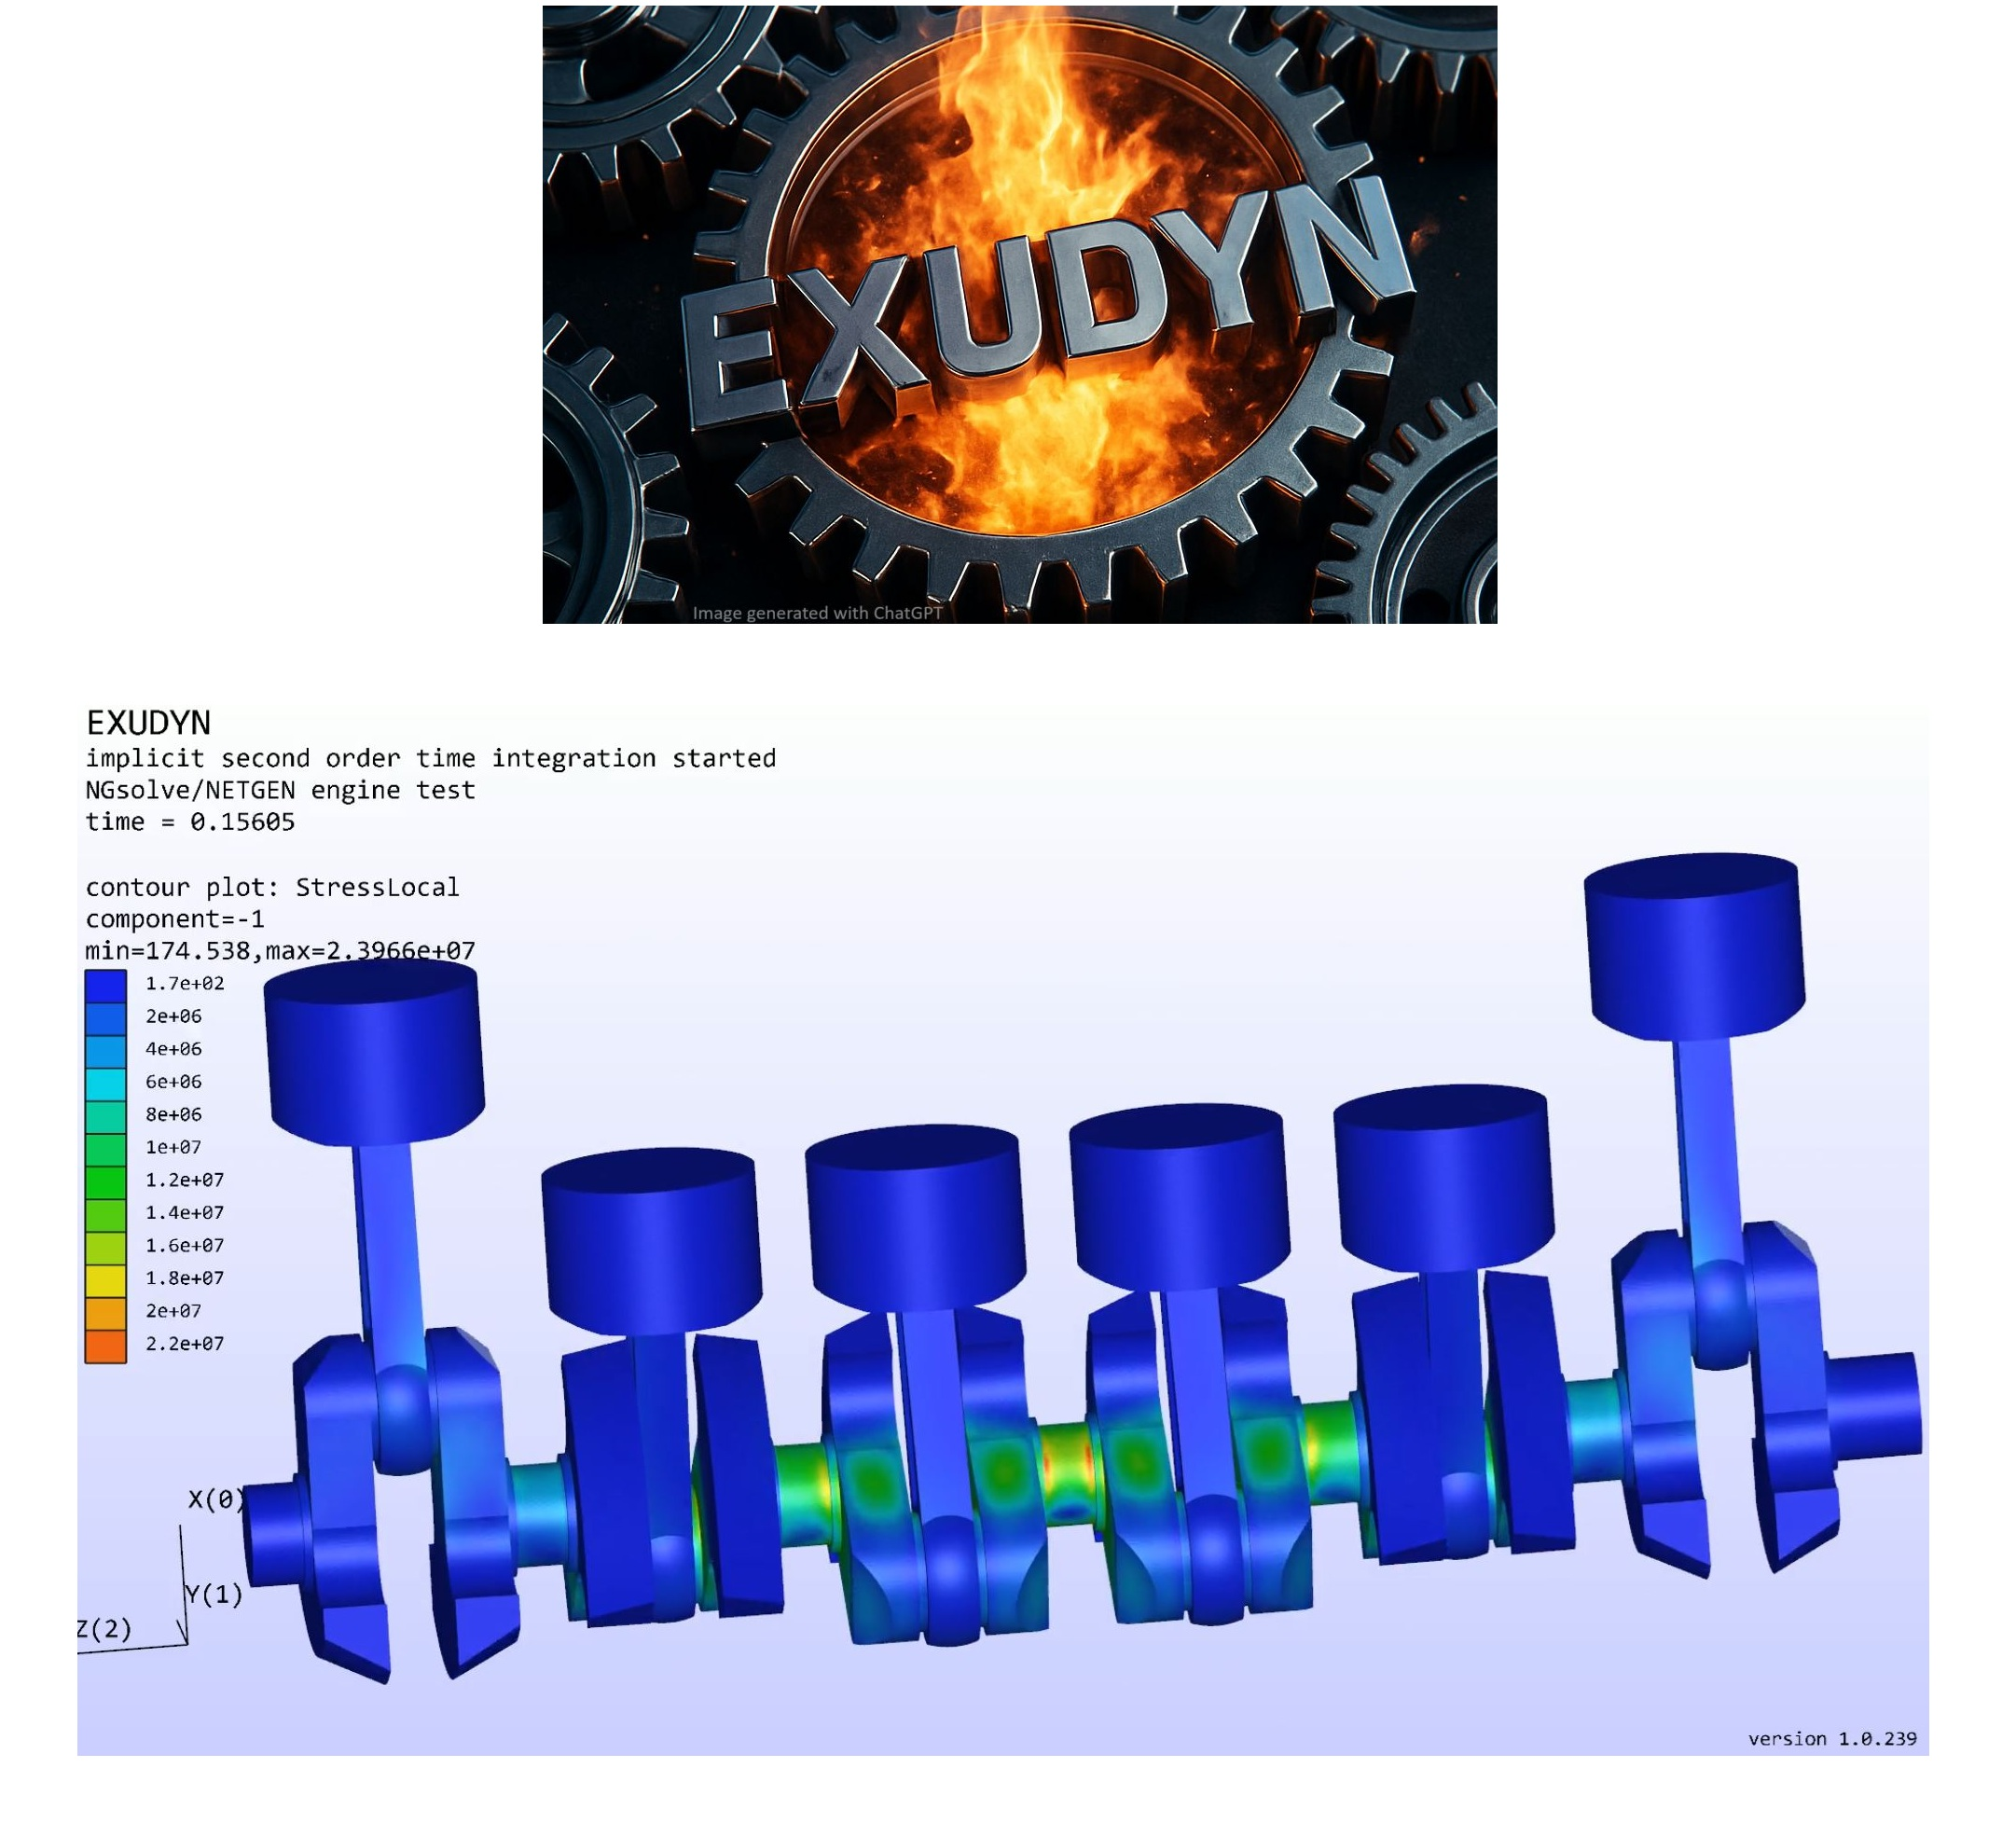
\includegraphics[height=14cm]{intro2.jpg}\\
	{\tiny (mesh and FEM-model generated with NETGEN and NGsolve -- 647058 total coordinates)}
\end{center}
\vspace{0.2cm}
{\small % version info automatically generated by tracker; generated by Johannes Gerstmayr
% last modified = 2022-05-18
Exudyn version = 1.2.86.dev1 (Corea)
}\\
{\small (build date and time=2022-03-21  15:23)}\\
{\small CHECK \refSection{sec:issueTracker} for changes from previous versions!!!\\}
\vspace{0.7cm}
University of Innsbruck, Department of Mechatronics, \today,\vspace{0.25cm}\\
Johannes Gerstmayr\vspace{1cm}
\end{center}

\newpage

\pagestyle{plain}
\headsep0.7cm 
%\headsep1cm 
%\chapter*{Contents}
%

%add additional entry for bookmarks in pdfs
\clearpage\phantomsection\pdfbookmark{\contentsname}{toc} 
%\setcounter{tocdepth}{3} %to add \mysubsubsubsection names
\tableofcontents

%%++++++++++++++++++++++++++++++++++++++++++++++
\clearpage
\pagenumbering{arabic} 
\setcounter{page}{0}

%++++++++++++++++++++++++++++++++++++++++++
\section*{List of abbreviations (for theDoc, C++ and Python codes)}
This section shows typical abbreviations. For further symbols in notation, see Section Notation \refSection{sec:generalnotation}.
\label{sec:listOfAbbreviations}
\begin{acronym}[coeffs] %put here longest acronym for list of acronyms
%unused: acro{ODE2t}[ODE2\_t]{velocities (or velocity terms) for second order ordinary differential equations}
\acro{2D}{two dimensions or planar}
\acro{3D}{three dimensions or spatial}
\acro{abs}{absolute (e.g., absolute error), absolute value}
\acro{AE}{algebraic equations}
\acro{CMS}{component mode synthesis}
\acro{coeffs}{coefficients}
\acro{COM}{center of mass}
\acro{DOF}{degree of freedom}
\acro{EOM}{equations of motion}
\acro{EP}{Euler parameters}
\acro{FFRF}{floating frame of reference formulation}
\acro{HT}{homogeneous transformation}
\acro{LHS}{Left-Hand-Side (of equation)}
\acro{LTG}{local-to-global}
\acro{mbs}{multibody system}
\acro{min}{minimum}
\acro{max}{maximum}
\acro{ODE}{ordinary differential equation}
\acro{ODE1}{first order ordinary differential equations}
\acro{ODE2}{second order ordinary differential equations}
\acro{pos}{position}
\acro{quad}{quadrangle, polygon with 4 vertices}
\acro{rel}{relative (e.g., relative error)}
\acro{RHS}{Right-Hand-Side (of equation)}
\acro{Rot}{rotation}
\acro{Rxyz}{rotation parameterization: consecutive rotations around x, y and z-axis (Tait-Bryan)}
\acro{STL}{STereoLithography}
\acro{T66}{Pl\"ucker transformation}
\acro{trig}{triangle}

% \acro{2D}{two dimensions or planar}
% \acro{3D}{three dimensions or spatial}
% \acro{abs}{absolute (e.g., absolute error), absolute value}
% \acro{AE}{algebraic equations}
% \acro{CMS}{component mode synthesis}
% \acro{coeffs}{coefficients}
% \acro{COM}{center of mass}
% \acro{EOM}{equations of motion}
% \acro{EP}{Euler parameters}
% \acro{FFRF}{floating frame of reference formulation}
% \acro{HT}{homogeneous transformation}
% \acro{LHS}{Left-Hand-Side (of equation)}
% \acro{LTG}{local-to-global}% 
% \acro{mbs}{multibody system}
% \acro{min}{minimum}
% \acro{max}{maximum}
% \acro{ODE}{ordinary differential equation}
% \acro{ODE1}{first order ordinary differential equations}
% \acro{ODE2}{second order ordinary differential equations}
% \acro{pos}{position}
% \acro{quad}{quadrangle, polygon with 4 vertices}
% \acro{rel}{relative (e.g., relative error)}
% \acro{RHS}{Right-Hand-Side (of equation)}
% \acro{Rot}{rotation}
% \acro{Rxyz}{rotation parameterization: consecutive rotations around x, y and z-axis (Tait-Bryan)}
% \acro{STL}{STereoLithography}
% \acro{T66}{Pl\"ucker transformation}
% \acro{trig}{triangle (in graphics)}
\end{acronym}
%use as: \ac{ODE2} %singular, or \acp for plural, \acf for repeated full name.

%+++++++++++++++++++++++++++++++++++++++++++++++++++++++++++++++++++++++++++++++
\iftoggle{compileAll}
{
%+++++++++++++++++++++++++++++++++++++++++++++++++++++++++++++++++++++++++++++++
\onlyRST{
+  **University of Innsbruck**, Austria, Department of Mechatronics

Exudyn now includes a redundant coordinate (constraint) as well as a minimum coordinate formulation (KinematicTree); machine learning and artificial intelligence interface (openAI gym); improved explicit and implicit solvers; sparse matrix support and multi-threading; creation of beams along curves; extended robotics modules; contact module; **PlotSensor** for simple post processing, ...   See theDoc.pdf chapter **Issues and Bugs** for changes!

If you like using Exudyn, please add a *star* on github, and send an email to \ ``reply.exudyn@gmail.com``\ such that we can add you to our newsletter. Let us know, which features you are using or which **features you are missing** and follow us on 
`Twitter @RExudyn <https://twitter.com/RExudyn>`_ !

A paper on Exudyn is planned to be presented at the `6th Joint International Conference on Multibody System Dynamics <http://imsdacmd2020.iitd.ac.in>`_

+  **A flexible multibody dynamics systems simulation code with Python and C++**
+  *free, open source* and with plenty of *documentation* and *examples*
+  **pre-built** for Python 3.6, 3.7, 3.8, 3.9, and 3.10 under **Windows** ; Python 3.8 for **MacOS** available; some **Linux** (UBUNTU wheels are available, but at most you should build your wheels by yourself, see instructions in `theDoc.pdf <https://github.com/jgerstmayr/EXUDYN/blob/master/docs/theDoc/theDoc.pdf>`_ )
+  **NOTE**: for pure installation, use **pip install exudyn** (see further description below)

.. |pic1| image:: docs/demo/screenshots/6pistonEngineStresses.jpg
   :width: 22%

.. |pic2| image:: docs/demo/screenshots/demo4piston.png
   :width: 14%

.. |pic3| image:: docs/demo/screenshots/shaftGear.png
   :width: 20%

.. |pic4| image:: docs/demo/screenshots/rotor_runup_plot3.png
   :width: 21%

.. |pic5| image:: docs/theDoc/figures/DrawSystemGraphExample.png
   :width: 21%

|pic1| |pic2| |pic3| |pic4| |pic5|

This README document is a small part of the complete documentation found as PDF document in docs/theDoc/theDoc.pdf.
It is auto-generated from .tex files (sorry for some conversion errors!). 
Due to limitations for complex formulas and tables in .rst files, details of the reference manual and many other parts of the documentation are only available in theDoc.pdf, see the `github page of Exudyn <https://github.com/jgerstmayr/EXUDYN/blob/master/docs/theDoc/theDoc.pdf>`_ !

For license, see LICENSE.txt in the root folder!

In addition to the tutorial in the documentation, many ( **100+** ) examples can be found under main/pythonDev/Examples and main/pythonDev/TestModels .

Tutorial videos can be found in the `youtube channel of Exudyn <https://www.youtube.com/playlist?list=PLZduTa9mdcmOh5KVUqatD9GzVg_jtl6fx>`_ !

Enjoy the Python library for multibody dynamics modeling, simulation, creating large scale systems, parameterized systems, component mode synthesis, optimization, ...
}
%
%.. image:: docs/theDoc/intro2.jpg
%    :width: 100%
%

\mysection{Installation and Getting Started}
\ignoreRST{
The documentation for \codeName\ is split into this introductory section, including a quick start up, code structure and important hints, 
as well as a couple of sections containing references to the available Python interfaces to interact with \codeName\ and finally some information on theory (e.g., 'Solver'). \vspace{6pt} \\
%
Tutorial videos can be found in the \exuUrl{https://www.youtube.com/playlist?list=PLZduTa9mdcmOh5KVUqatD9GzVg_jtl6fx}{youtube channel of Exudyn}.
}
%
\noindent \codeName\ is hosted on \exuUrl{https://github.com}{GitHub} \cite{EXUDYNgit}:
\bi
  \item web: \exuUrl{https://github.com/jgerstmayr/EXUDYN}{https://github.com/jgerstmayr/EXUDYN}
\ei
%
For any comments, requests, issues, bug reports, send an email to: 
\bi
  \item email: \texttt{reply.exudyn@gmail.com}
\ei
Thanks for your contribution!

\mysubsection{Getting started}
This section will show:
\bn
  \item What is \codeName ?
  \item Who is developing \codeName ?
  \item How to install \codeName\ 
  \item How to link \codeName\ and Python
  \item Goals of \codeName
  \item Run a simple example in Python
  \item FAQ -- Frequently asked questions
\en

\mysubsubsection{What is \codeName ?}
\codeName -- {\small (fl\mybold{EX}ible m\mybold{U}ltibody \mybold{DYN}amics  -- \mybold{EX}tend yo\mybold{U}r \mybold{DYN}amics)}\vspace{6pt}\\
\noindent \codeName\ is a C++ based Python library for efficient simulation of flexible multibody dynamics systems.
It is the follow up code of the previously developed multibody code HOTINT, which Johannes Gerstmayr started during his PhD-thesis.
It seemed that the previous code HOTINT reached limits of further (efficient) development and it seemed impossible to continue from this code as it was outdated regarding programming techniques and the numerical formulation at the time \codeName\ was started.

\codeName\ is designed to easily set up complex multibody models, consisting of rigid and flexible bodies with joints, loads and other components. It shall enable automatized model setup and parameter variations, which are often necessary for system design but also for analysis of technical problems. The broad usability of Python allows to couple a multibody simulation with environments such as optimization, statistics, data analysis, machine learning and others.

The multibody formulation is mainly based on redundant coordinates. This means that computational objects (rigid bodies, flexible bodies, ...) are added as independent bodies to the system. Hereafter, connectors (e.g., springs or constraints) are used to interconnect the bodies. The connectors are using Markers on the bodies as interfaces, in order to transfer forces and displacements.
For details on the interaction of nodes, objects, markers and loads see \refSection{sec:items}.

\mysubsubsection{Developers of \codeName\ and thanks}
\codeName\ is currently (\the\month-\the\year) developed at the University of Innsbruck.
In the first phase most of the core code is written by Johannes Gerstmayr, implementing ideas that followed out of the project HOTINT \cite{GerstmayrEtAl2013}. 15 years of development led to a lot of lessons learned and after 20 years, a code must be re-designed.

Some important tests for the coupling between C++ and Python have been written by Stefan Holzinger. Stefan also helped to set up the previous upload to GitLab and to test parallelization features.
For the interoperability between C++ and Python, we extensively use \mybold{Pybind11}\cite{pybind11}, originally written by Jakob Wenzel, see \texttt{https://github.com/pybind/pybind11}. Without Pybind11 we couldn't have made this project -- Thanks a lot!

Important discussions with researchers from the community were important for the design and development of \codeName , where we like to mention Joachim Sch{\"o}berl from TU-Vienna who boosted the design of the code with great concepts. 
%During a Comet-K2 cooperation project, several discussions with the TMECH/LCM group in Linz influenced the code development.

The cooperation and funding within the EU H2020-MSCA-ITN project 'Joint Training on Numerical Modelling of Highly Flexible Structures for Industrial Applications' contributes to the development of the code.

The following people have contributed to Python and C++ library implementations:
\bi
  \item Joachim Sch{\"o}berl, TU Vienna (Providing specialized NGsolve \cite{Schoeberl1997,Schoeberl2014,2022NGsolve} core library with \texttt{taskmanager} for \mybold{multi-threaded parallelization}; NGsolve mesh and FE-matrices import; highly efficient eigenvector computations)
  \item Stefan Holzinger, University of Innsbruck (Lie group solvers in Python, Lie group node)
  \item Andreas Zw{\"o}lfer, Technical University Munich (FFRF and CMS formulation)
  \item Peter Manzl, University of Innsbruck (ConvexRoll Python and C++ implementation / pip install on linux / wsl with graphics)
  \item Martin Sereinig, University of Innsbruck (special robotics functionality)
  \item Grzegorz Orzechowski, Lappeenranta University of Technology (coupling with openAI gym and running machine learning algorithms)
\ei
The following people have contributed to examples and other parts:
\bi
  \item Stefan Holzinger, Michael Pieber, Manuel Schieferle, Martin Knapp, Lukas March, Dominik Sponring, David Wibmer, Andreas Zw{\"o}lfer, Peter Manzl, Simon Scheiber
\ei
-- thanks a lot! --
%
%++++++++++++++++++++++++++++++++++++++++++++++++++++++++++++++++
%++++++++++++++++++++++++++++++++++++++++++++++++++++++++++++++++
%++++++++++++++++++++++++++++++++++++++++++++++++++++++++++++++++
\newpage
\mysubsection{Installation instructions}
\label{sec:installationInstructions}
%
\mysubsubsection{Requirements for \codeName ?}

\codeName\ only works with Python. Thus, you need an appropriate Python installation.
So far (2021-07), we tested
\bi
  \item \mybold{Anaconda, 64bit, Python 3.7.7}\footnote{Anaconda3 64bit with Python3.7.7 can be downloaded via the repository archive \texttt{https://repo.anaconda.com/archive/} choosing \texttt{Anaconda3-2020.02-Windows-x86\_64.exe}} (but Python 3.8 and 3.9 (since 2021-11) are also working well!)
  \item \mybold{Spyder 4.1.3} (with Python 3.7.7, 64bit), which is included in the Anaconda installation\footnote{It is important that Spyder, Python and \codeName\  are \mybold{either} 32bit \mybold{or} 64bit and are compiled up to the same minor version, i.e., 3.7.x. There will be a strange .DLL error, if you mix up 32/64bit. It is possible to install both, Anaconda 32bit and Anaconda 64bit -- then you should follow the recommendations of paths as suggested by Anaconda installer.}
\ei
Many alternative options exist:
\bi
  \item In case that you have an older CPU, which does not support AVX2, use: \codeName\ with Python 3.6.5, or compile without AVX flags for your machine.\footnote{e.g.\ Anaconda 32bit with Python3.6 can be downloaded via the repository archive \texttt{https://repo.anaconda.com/archive/} choosing \texttt{Anaconda3-5.2.0-Windows-x86.exe}.}
  %\item Spyder 3.2.8 with Python 3.6.5 32 bit (alternatively 64bit), which is included in the Anaconda installation\footnote{It is important that Spyder, Python and exudyn are \mybold{either} 32bit \mybold{or} 64bit. 
  \item Users report successful use of \codeName\ with \mybold{Visual Studio Code}. \mybold{Jupyter} has been tested with some examples; both environments should work with default settings.
  \item Anaconda 2020-11 with \mybold{Python 3.8} and Spyder 4.1.5: no problems up to now (2021-07), TestSuite runs without problems since \codeName\ version 1.0.182.
  \item Anaconda 2021-11 with \mybold{Python 3.9} and Spyder 5.1.5: Tested with current version (1.1.99), TestSuite runs without problems.
  \item Alternative option with more stable Spyder (as compared to Spyder 4.1.3): Anaconda, 64bit, Python 3.6.5)\footnote{Anaconda 64bit with Python3.6 can be downloaded via the repository archive \texttt{https://repo.anaconda.com/archive/} choosing \texttt{Anaconda3-5.2.0-Windows-x86\_64.exe} for 64bit.}
  %\item Spyder 3.2.8 with Python 3.6.5 32 bit (alternatively 64bit), which is included in the Anaconda installation\footnote{It is important that Spyder, Python and exudyn are \mybold{either} 32bit \mybold{or} 64bit. 
%Anaconda3-5.2.0-Windows-x86\_64.exe
\ei
If you plan to extend the C++ code, we recommend to use VS2017\footnote{previously, VS2019 was recommended: However, VS2019 has problems with the library 'Eigen' and therefore leads to erroneous results with the sparse solver. VS2017 can also be configured with Python 3.7 now.} to compile your code, which offers Python 3.7 compatibility.
Once again, remember that Python versions and the version of the \codeName\ module must be identical (e.g., Python 3.6 32 bit \mybold{both} in the \codeName\ module and in Spyder).

\paragraph{Run without Anaconda:}
If you do not install Anaconda (e.g., under Linux), make sure that you have the according Python packages installed:
\bi
  \item \texttt{numpy} (used throughout the code, inevitable)
  \item \texttt{matplotlib} (for any plot, also PlotSensor(...))
  \item \texttt{tkinter} (for interactive dialogs, SolutionViewer, etc.)
  \item \texttt{scipy} (needed for eigenvalue computation)
\ei
You can install most of these packages using \texttt{pip install numpy} (Windows) or \texttt{pip3 install numpy} (Linux).

For interaction (right-mouse-click, some key-board commands) you need the Python module \texttt{tkinter}. This is included in regular Anaconda distributions (recommended, see below), but on UBUNTU you need to type alike (do not forget the '3', otherwise it installs for Python2 ...):
\bi
  \item[] \texttt{sudo apt-get install python3-tk}
\ei
see also common blogs for your operating system.

%+++++++++++++++++++++++++++++++++++++
\mysubsubsection{Install \codeName\ with PIP INSTALLER (pypi.org)}
Pre-built versions of \codeName\ are hosted on \texttt{pypi.org}, see the project
\bi
 \item \exuUrl{https://pypi.org/project/exudyn}{https://pypi.org/project/exudyn}
\ei
As with most other packages, in the regular case (if your binary has been pre-built) you just need to do\footnote{If the index of pypi is not updated, it may help to use \texttt{pip install -i https://pypi.org/project/ exudyn} }
\bi
  \item[] \texttt{pip install exudyn}
\ei
On Linux (currently only pre-built for UBUNTU 18.04 and 20.04), {\bf update pip to at least 20.3} and use 
\bi
  \item[] \texttt{pip3 install exudyn}
\ei
For pre-releases (use with care!), add '$--$pre' flag:
\bi
  \item[] \texttt{pip install exudyn $--$pre}
\ei
In some cases (e.g. for AppleM1), your pre-built binary will not work due to some incompatibilities. Then you need to build from source as described in the 'Build and install' sections, \refSection{sec:build:windows}.

%+++++++++++++++++++++++++++++++++++++
\mysubsubsection{DEPRECATED: Install with Windows MSI installer}
A simple way to install \codeName\ on Windows 10 (and maybe also Windows 7) is to use \texttt{.msi} installers in the \texttt{main/dist} directory\footnote{It works better \mybold{if you installed only one Python version} and if you installed Anaconda with the option \mybold{'Register Anaconda as my default Python 3.x'} or similar; in other cases you may to specify some installation directories, etc.}:
\bi
  \item NOTE (2022-03-18): \texttt{.msi} installers are now only available for selected Python versions; however, wheels can be downloaded directly from \exuUrl{https://pypi.org/project/exudyn}{https://pypi.org/project/exudyn}, see below
  \item For the 64bits Python 3.7 version, double click on (version may differ):\ignoreRST{\\} \texttt{exudyn-1.0.248.win-amd64-py3.7.msi}
  \item Follow the instructions of the installer
  \item If Python / Anaconda is not found by the installer, provide the 'Python directory' as the installation directory of Anaconda3, which usually is installed in:\\
  \texttt{C:$\backslash$ProgramData$\backslash$Anaconda3}
\ei

%+++++++++++++++++++++++++++++++++++++
\mysubsubsection{Install from Wheel (UBUNTU and Windows)}
A way to install the Python package \codeName\ is to use the so-called 'wheels' (file ending \texttt{.whl}).
Wheels can be downloaded directly from \exuUrl{https://pypi.org/project/exudyn/\#files}{https://pypi.org/project/exudyn/\#files}, for many Python versions and architectures.
\vspace{6pt}\\
For UBUNTU18.04 (which by default uses Python 3.6) this may read (version number 1.0.20 may be different):
\bi
  \item \texttt{Python 3.6, 64bit}: pip3 install dist$\backslash$exudyn-1.0.20-cp36-cp36-linux\_x86\_64.whl
\ei
For UBUNTU20.04 (which by default uses Python 3.8) this may read (version number 1.0.20 may be different):
\bi
  \item \texttt{Python 3.8, 64bit}: pip3 install dist$\backslash$exudyn-1.0.20-cp38-cp38-linux\_x86\_64.whl
\ei
NOTE that your installation may have environments with different Python versions, so install that \codeName\ version appropriately!
If the wheel installation does not work on UBUNTU, it is highly recommended to build \codeName\ for your specific system as given in \refSection{sec:build:ubuntu}.

\noindent \mybold{Windows}:\vspace{6pt}\\
First, open an Anaconda prompt:
\bi
  \item EITHER calling: START->Anaconda->... OR go to anaconda/Scripts folder and call activate.bat
  \item You can check your Python version then, by running \texttt{python}\footnote{\texttt{python3} under UBUNTU 18.04}, the output reads like:
  \bi
    \item[] \texttt{Python 3.6.5 $|$Anaconda, Inc.$|$ (default, Mar 29 2018, 13:32:41) $[$MSC v.1900 64 bit (AMD64)$]$ on win32}
    \item[] ...
  \ei
  \item type \texttt{exit()} to close Python
\ei
%
%\noindent \mybold{Go to the folder} \texttt{Exudyn\_git/main} (where \texttt{setup.py} lies) and choose the wheel in subdirectory \texttt{main/dist} according to your system (windows/UBUNTU), Python version (3.6 or 3.7) and 32 or 64 bits.
%
For Windows the installation commands may read (version number 1.0.20 may be different):
\bi
  \item \texttt{Python 3.6, 32bit}: pip install dist$\backslash$exudyn-1.0.20-cp36-cp36m-win32.whl
  \item \texttt{Python 3.6, 64bit}: pip install dist$\backslash$exudyn-1.0.20-cp36-cp36m-win\_amd64.whl
  \item \texttt{Python 3.7, 64bit}: pip install dist$\backslash$exudyn-1.0.20-cp37-cp37m-win\_amd64.whl
\ei

%%+++++++++++++++++++++++++++++++++++++
%\mysubsubsection{Work without installation and editing \texttt{sys.path}}
%The \mybold{uncommon and old way} ($\ra$ not recommended for \codeName\ versions $\ge$ 1.0.0) is to use Python's \texttt{sys} module to link to your \texttt{exudyn} (previously \texttt{WorkingRelease}) directory, for example:
%\pythonstyle\begin{lstlisting}
  %import sys
  %sys.path.append('C:/DATA/cpp/EXUDYN_git/bin/EXUDYN32bitsPython36')
%\end{lstlisting}
%
%The folder \texttt{EXUDYN32bitsPython36} needs to be adapted to the location of the according \codeName\ package.
%In case of 64bit, it must be changed to \texttt{.... /bin/WorkingRelease64}.

%In the future, there will also be a possibility to install the module using pip commands -- we are happy, if somebody could do this!

%++++++++++++++++++++++++++++++++++++++++++++++++++++++++++++++++++++++++++++++
%++++++++++++++++++++++++++++++++++++++++++++++++++++++++++++++++++++++++++++++
\mysubsubsection{Build and install \codeName\ under Windows 10?}
\label{sec:build:windows}
Note that there are a couple of pre-requisites, depending on your system and installed libraries. For Windows 10, the following steps proved to work:
\bi
  \item you need an appropriate compiler (tested with Microsoft Visual Studio; recommended: VS2017)
  \item install your Anaconda distribution including Spyder
  \item close all Python programs (e.g. Spyder, Jupyter, ...) 
  \item run an Anaconda prompt (may need to be run as administrator)
  \item if you cannot run Anaconda prompt directly, do:
  \bi
    \item open windows shell (cmd.exe) as administrator (START $\ra$ search for cmd.exe $\ra$ right click on app $\ra$ 'run as administrator' if necessary) [may not be necessary]
    \item go to your Scripts folder inside the Anaconda folder (e.g. \texttt{C:$\backslash$ProgramData$\backslash$Anaconda$\backslash$Scripts}) [may not be necessary]
    \item run 'activate.bat' [may not be necessary]
  \ei
  \item go to 'main' of your cloned github folder of \codeName\ 
  \item run: \texttt{python setup.py install}
  \item read the output; if there are errors, try to solve them by installing appropriate modules
\ei
You can also create your own wheels, doing the above steps to activate the according Python version and then calling:
\bi
  \item[] \texttt{python setup.py bdist\_wheel}
\ei
This will add a wheel in the \texttt{dist} folder.

%++++++++++++++++++++++++++++++++++++++++++++++++++++++++++++++++++++++++++++++
%++++++++++++++++++++++++++++++++++++++++++++++++++++++++++++++++++++++++++++++
\mysubsubsection{Build and install \codeName\ under Mac OS X?}
\label{sec:build:MacOS}
Installation and building on Mac OS X is rarely tested, but first successful compilation including GLFW has been achieved.
Requirements are an according Anaconda (or Miniconda) installation.

\noindent \mybold{Tested configurations}:
\bi
  \item Mac OS 11.x 'Big Sur', Mac Mini (2021), Apple M1, 16GB Memory
  \item Anaconda (x86 / i368 based with Rosetta 2) with Python 3.8
  \item this configuration is currently evaluated but showed general compatibility
  \item[] $\ra$ some wheels are already available on pypi (you may need to download them manually)!
\ei
\noindent \mybold{NOTE}:
\bi
  \item on Apple M1 processors, there are significant problems with Miniconda; scipy cannot be installed properly (April 2022)
  \item a significant number of Exudyn test models does not run properly! Optimization and processing functions do not run (especially multiprocessing and tqdm); 
  \item as eigensolvers were not available for tests on M1, all these test models fail 
  \item note that even some test result deviate from Windows results significantly!
\ei


Alternatively, we tested on:
\bi
  \item Mac OS X 10.11.6 'El Capitan', Mac Pro (2010), 3.33GHz 6-Core Intel Xeon, 4GB Memory, Anaconda Navigator 1.9.7, Python 3.7.0, Spyder 3.3.6
\ei
Note, that in all cases tkinter does not run properly on MacOS (help appreciated), while otherwise we produced a stable version. The AppleM1 native version is in some cases superior to the Windows version and also to the Rosetta version on Apple!

For a compatible Mac OS X system some pre-built wheels will be available via pypi.org. Note that these my be built on an emulated AppleM1, thus being much slower than the Windows or Linux compliant.
%Go to the \texttt{main/dist} directory in your back terminal and type, e.g.,
%\bi
%\item[] \texttt{pip install exudyn-1.0.218-cp37-cp37m-macosx\_10\_9\_x86\_64.whl} %\vspace{9pt}\\
%\ei
%
\vspace{9pt}
\mybold{Compile from source}:\vspace{3pt}\\
If you would like to compile from source, just use a bash terminal on your Mac, and do the following steps inside the \texttt{main} directory of your repository and type
\bi
  \item uninstall if old version exists (may need to repeat this!): \texttt{pip uninstall exudyn}
  \item \texttt{python setup.py bdist\_wheel}
  \item[] $\ra$ this compiles and takes approx.~5 minutes, depending on your machine
  \item[] $\ra$ it may produce some errors, depending on your version; if there are some liker errors (saying that there is no '\texttt{-framework Cocoa' and '-framework OpenGL}', just go back in the terminal and copy everything from '\texttt{g++ ...}' until the end of the last command '\texttt{-mmacosx-verion-min...}' and paste it into the terminal. Calling that again will finalize linking; then run again
  \item[] \texttt{python setup.py bdist\_wheel}
  \item[] $\ra$ this now creates the wheel (if you want to distribute) in the \texttt{dist} folder; note that this wheel has a wrong version number (11.0) while it may need to be changed to 10.9 manually in order that it can be installed
  \item \texttt{python setup.py install}
  \item[] to install exudyn
\ei
Then just go to the \texttt{pythonDev/Examples} folder and run an example:
\bi
  \item[] \texttt{python springDamperUserFunctionTest.py}
\ei
If there are other issues, we are happy to receive your detailed bug reports. 

\noindent Note that you need to run 
\bi
\item[] \texttt{exudyn.StartRenderer()}
\item[] \texttt{exudyn.DoRendererIdleTasks(-1)}
\ei
in order to interact with the render window, as there is only a single-threaded version available for Mac OS.

%++++++++++++++++++++++++++++++++++++++++++++++++++++++++++++++++++++++++++++++
%++++++++++++++++++++++++++++++++++++++++++++++++++++++++++++++++++++++++++++++
\mysubsubsection{Build and install \codeName\ under UBUNTU?}
\label{sec:build:ubuntu}
Having a new UBUNTU 18.04 standard installation (e.g. using a VM virtual box environment), the following steps need to be done (Python \mybold{3.6} is already installed on UBUNTU18.04, otherwise use \texttt{sudo apt install python3})\footnote{see also the youtube video: \exuUrl{https://www.youtube.com/playlist?list=PLZduTa9mdcmOh5KVUqatD9GzVg\_jtl6fx}{https://www.youtube.com/playlist?list=PLZduTa9mdcmOh5KVUqatD9GzVg\_jtl6fx}}:

\noindent First update ...
\plainlststyle
\begin{lstlisting}
  sudo apt-get update
\end{lstlisting}

\noindent 
Install necessary Python libraries and pip3; \texttt{matplotlib} and\texttt{scipy} are not required for installation but used in \codeName\ examples:
\begin{lstlisting}
  sudo dpkg --configure -a
  sudo apt install python3-pip
  pip3 install numpy
  pip3 install matplotlib
  pip3 install scipy
\end{lstlisting}

\noindent Install pybind11 (needed for running the setup.py file derived from the pybind11 example):
\begin{lstlisting}
  pip3 install pybind11
\end{lstlisting}

\noindent 
If graphics is used (\texttt{\#define USE\_GLFW\_GRAPHICS} in \texttt{BasicDefinitions.h}), you must install the according GLFW and OpenGL libs:
\begin{lstlisting}
  sudo apt-get install freeglut3 freeglut3-dev
  sudo apt-get install mesa-common-dev
  sudo apt-get install libglfw3 libglfw3-dev
  sudo apt-get install libx11-dev xorg-dev libglew1.5 libglew1.5-dev libglu1-mesa libglu1-mesa-dev libgl1-mesa-glx libgl1-mesa-dev
\end{lstlisting}

\noindent 
With all of these libs, you can run the setup.py installer (go to \texttt{Exudyn\_git/main} folder), which takes some minutes for compilation (the --user option is used to install in local user folder):
\begin{lstlisting}
  sudo python3 setup.py install --user
\end{lstlisting}

\noindent 
Congratulation! \mybold{Now, run a test example} (will also open an OpenGL window if successful):
\bi
  \item[] \texttt{python3 pythonDev/Examples/rigid3Dexample.py}
\ei

\noindent You can also create a UBUNTU wheel which can be easily installed on the same machine (x64), same operating system (UBUNTU18.04) and with same Python version (e.g., 3.6):
\bi
  \item[] \texttt{sudo pip3 install wheel}
  \item[] \texttt{sudo python3 setup.py bdist\_wheel}
\ei

\noindent \mybold{Exudyn under Ubuntu / WSL}:
\bi
  \item Note that \codeName\ also nicely works under WSL (Windows subsystem for linux; tested for Ubuntu18.04) and an according xserver (VcXsrv).
  \item Just set the display variable in your .bashrc file accordingly and you can enjoy the OpenGL windows and settings.
  \item It shall be noted that WSL + xserver works better than on MacOS, even for tkinter, multitasking, etc.! So, if you have troubles with your Mac, use a virtual machine with ubuntu and a xserver, that may do better
\ei

\noindent \mybold{Exudyn under Raspberry Pi 4b}:
\bi
  \item Exudyn also compiles under RaspberryPi 4b, Ubuntu Mate 20.04, Python 3.8; current version should compile out of the box using \texttt{python3 setup.py install} command.
  \item Performance is quite ok and it is even capable to use all cores (but you should add a fan!)
  \item $\ra$ this could lead to a nice cluster project!
\ei

\noindent \mybold{KNOWN issues for linux builds}:
\bi
  \item Using \mybold{WSL2} (Windows subsystem for linux), there occur some conflicts during build because of incompatible windows and linux file systems and builds will not be copied to the dist folder; workaround: go to explorer, right click on 'build' directory and set all rights for authenticated user to 'full access'
  \item \mybold{compiler (gcc,g++) conflicts}: It seems that \codeName works well on UBUNTU18.04 with the original \texttt{Python 3.6.9} and \texttt{gcc-7.5.0} version as well as with UBUNTU20.04 with \texttt{Python 3.8.5} and \texttt{gcc-9.3.0}. Upgrading \texttt{gcc} on a linux system with Python 3.6 to, e.g., \texttt{gcc-8.2} showed us a linker error when loading the \codeName\ module in Python -- there are some common restriction using \texttt{gcc} versions different from those with which the Python version has been built. Starting \texttt{python} or \texttt{python3} on your linux machine shows you the \texttt{gcc} version it had been build with. Check your current \texttt{gcc} version with: \texttt{gcc --version}
\ei

%++++++++++++++++++++++++++++++++++++++++++++++++++++++++++++++++++++++++++++++
\mysubsubsection{Uninstall \codeName }

To uninstall exudyn under Windows, run (may require admin rights):
\bi
  \item[] \texttt{pip uninstall exudyn}
\ei
\noindent To uninstall under UBUNTU, run:
\bi
  \item[] \texttt{sudo pip3 uninstall exudyn}
\ei

If you upgrade to a newer version, uninstall is usually not necessary!
%
%++++++++++++++++++++++++++++++++++++++++++++++++++++++++++++++++

\mysubsubsection{How to install \codeName\ and use the C++ source code (advanced)?}
\codeName\ is still under intensive development of core modules.
There are several ways of using the code, but you \mybold{cannot} install \codeName\ as compared to other executable programs and apps.
\vspace{6pt}\\
%\mybold{Ways to use \codeName }:
In order to make full usage of the C++ code and extending it, you can use:
\bi
  \item Windows / Microsoft Visual Studio 2017 and above:
  \bi
    \item get the files from git
    \item put them into a local directory (recommended: \texttt{C:/DATA/cpp/EXUDYN\_git})
    \item start \texttt{main\_sln.sln} with Visual Studio
    \item compile the code and run \texttt{main/pythonDev/pytest.py} example code
    \item adapt \texttt{pytest.py} for your applications
    \item extend the C++ source code
    \item link it to your own code
    \item NOTE: on Linux systems, you mostly need to replace '$/$' with '$\backslash$'
  \ei
  \item Linux, etc.: not fully supported yet; however, all external libraries are Linux-compatible and thus should run with minimum adaptation efforts.
\ei
%
%++++++++++++++++++++++++++++++++++++++++++++++++++++++++++++++++
%++++++++++++++++++++++++++++++++++++++++++++++++++++++++++++++++
\mysubsection{Further notes}
\mysubsubsection{Goals of \codeName}
After the first development phase (2019-2021), it
\bi
  \item is a moderately large (2MB on windows!) multibody library, which can be easily linked to other projects,
  \item contains basic multibody rigid bodies, flexible bodies, joints, contact, etc.,
  \item includes a large Python utility library for convenient building and post processing of models,
  \item allows to efficiently simulate small scale systems (compute $100\,000$s of time steps per second for systems with $n_{DOF}<10$),
  \item allows to efficiently simulate medium scaled systems for problems with $n_{DOF} < 1\,000\,000$,
  \item is a safe and widely accessible module for Python,
  \item allows to add user defined objects and solvers in C++,
  \item allows to add user defined objects and solvers in Python.
\ei
Future goals are:
\bi
  \item add more multi-threaded parallel computing techniques (first parts implemented, improvements planned during 2022),
  \item add vectorization,
  \item add specific and advanced connectors/constraints (extended wheels, contact, control connector)
  \item kinematical trees (with minimum coordinates),
  \item automatic step size selection for second order solvers,
  \item deeper integration of Lie groups,
  \item more interfaces for robotics,
  \item add 3D beams.
\ei
For solved issues (and new features), see section 'Issues and Bugs', \refSection{sec:issueTracker}.
For specific open issues, see \texttt{trackerlog.html} -- a document only intended for developers!
%
%++++++++++++++++++++++++++++++++++++++++++++++++++++++++++++++++
%++++++++++++++++++++++++++++++++++++++++++++++++++++++++++++++++
\mysubsection{Run a simple example in Python}
After performing the steps of the previous section, this section shows a simplistic model which helps you to check if \codeName\ runs on your computer.

In order to start, run the Python interpreter Spyder (or any preferred Python environment).
For the following example, 
\bi
\ignoreRST{
\item open Spyder and copy the example provided in Listing \ref{lst:firstexample} into a new file, or}
\item open \texttt{myFirstExample.py} from your \texttt{Examples} folder.
\ei
Hereafter, press the play button or \texttt{F5} in Spyder.
%\lstinputlisting[language=Python]{../../main/bin/WorkingRelease/myFirstExample.py}
\ignoreRST{
\pythonexternal[language=Python, frame=single, float, label=lst:firstexample, caption=My first example]{../../main/pythonDev/Examples/myFirstExample.py}
}

If successful, the IPython Console of Spyder will print something like:
\begin{lstlisting}
  runfile('C:/DATA/cpp/EXUDYN_git/main/pythonDev/Examples/myFirstExample.py', 
    wdir='C:/DATA/cpp/EXUDYN_git/main/pythonDev/Examples')
  +++++++++++++++++++++++++++++++
  EXUDYN V1.2.9 solver: implicit second order time integration
  STEP100, t = 1 sec, timeToGo = 0 sec, Nit/step = 1
  solver finished after 0.0007824 seconds.
\end{lstlisting}
  %runfile('C:/DATA/cpp/EXUDYN_git/main/bin/WorkingRelease/myFirstExample.py', 
    %wdir='C:/DATA/cpp/EXUDYN_git/main/bin/WorkingRelease')

If you check your current directory (where \texttt{myFirstExample.py} lies), you will find a new file \texttt{coordinatesSolution.txt}, which contains the results of your computation (with default values for time integration).
The beginning and end of the file should look like: \vspace{6pt}\\
\begin{lstlisting}
  #Exudyn implicit second order time integration solver solution file
  #simulation started=2022-04-07,19:02:19
  #columns contain: time, ODE2 displacements, ODE2 velocities, ODE2 accelerations
  #number of system coordinates [nODE2, nODE1, nAlgebraic, nData] = [2,0,0,0]
  #number of written coordinates [nODE2, nVel2, nAcc2, nODE1, nVel1, nAlgebraic, nData] = [2,2,2,0,0,0,0]
  #total columns exported  (excl. time) = 6
  #number of time steps (planned) = 100
  #Exudyn version = 1.2.33.dev1; Python3.9.11; Windows AVX2 FLOAT64
  #
  0,0,0,0,0,0.0001,0
  0.01,5e-09,0,1e-06,0,0.0001,0
  0.02,2e-08,0,2e-06,0,0.0001,0
  0.03,4.5e-08,0,3e-06,0,0.0001,0
  0.04,8e-08,0,4e-06,0,0.0001,0
  0.05,1.25e-07,0,5e-06,0,0.0001,0

  ...

  0.96,4.608e-05,0,9.6e-05,0,0.0001,0
  0.97,4.7045e-05,0,9.7e-05,0,0.0001,0
  0.98,4.802e-05,0,9.8e-05,0,0.0001,0
  0.99,4.9005e-05,0,9.9e-05,0,0.0001,0
  1,5e-05,0,0.0001,0,0.0001,0
  #simulation finished=2022-04-07,19:02:19
  #Solver Info: stepReductionFailed(or step failed)=0,discontinuousIterationSuccessful=1,newtonSolutionDiverged=0,massMatrixNotInvertible=1,total time steps=100,total Newton iterations=100,total Newton jacobians=100
\end{lstlisting}
%
Within this file, the first column shows the simulation time and the following columns provide coordinates, their derivatives and Lagrange multipliers on system level. For relation of local to global coordinates, see \refSection{sec:systemData:LTG}. As expected, the $x$-coordinate of the point mass has constant acceleration $a=f/m=0.001/10=0.0001$, the velocity grows up to $0.0001$ after 1 second and the point mass moves $0.00005$ along the $x$-axis.

Note that line 8 contains the \codeName\ and Python versions\footnote{as well as some other specific information on the platform and compilation settings (which may help you identify with which computer, etc., you created results)} provided in the solution file are the versions at which Exudyn has been compiled with.
The Python micro version (last digit) may be different from the Python version from which you were running Exudyn.
This information is also provided in the sensor output files.
%
%++++++++++++++++++++++++++++++++++++++++++++++++++++++++++++++++
%++++++++++++++++++++++++++++++++++++++++++++++++++++++++++++++++
\newpage
\mysubsection{Trouble shooting and FAQ}

\mysubsubsection{Trouble shooting}
\noindent \mybold{Python import errors}:
\bi
  %++++++++++++++++++++++++++++++++++++++++++++++++++++++++++++++++++++++++++++++++++++++++
  %++++++++++++++++++++++++++++++++++++++++++++++++++++++++++++++++++++++++++++++++++++++++
  \item Sometimes the \codeName\ module cannot be loaded into Python. Typical \mybold{error messages if Python versions are not compatible} are: \vspace{1pt}\\
\plainlststyle
\begin{lstlisting}
  Traceback (most recent call last):

    File "<ipython-input-14-df2a108166a6>", line 1, in <module>
      import exudynCPP

  ImportError: Module use of python36.dll conflicts with this version of Python.
\end{lstlisting}
%
  Typical \mybold{error messages if 32/64 bits versions are mixed}:\vspace{1pt}\\
\begin{lstlisting}
  Traceback (most recent call last):
  
    File "<ipython-input-2-df2a108166a6>", line 1, in <module>
      import exudynCPP

  ImportError: DLL load failed: \%1 is not a valid Win32 application.
\end{lstlisting}
%
  \mybold{There are several reasons and workarounds}:
\bi
\item[$\ra$] You mixed up 32 and 64 bits version (see below) 
\item[$\ra$] You are using an exudyn version for Python $x_1.y_1$ (e.g., 3.6.$z_1$) different from the Python $x_2.y_2$ version in your Anaconda (e.g., 3.7.$z_2$); note that $x_1=x_2$ and $y_1=y_2$ must be obeyed while $z_1$ and $z_2$ may be different
\ei
\item \mybold{ModuleNotFoundError: No module named 'exudynCPP'}:\\
\bi
\item[$\ra$] A known reason is that your CPU \mybold{does not support AVX2}, while \codeName\ is compiled with the AVX2 option\footnote{modern Intel Core-i3, Core-i5 and Core-i7 processors as well as AMD processors, especially Zen and Zen-2 architectures should have no problems with AVX2; however, low-cost Celeron, Pentium and older AMD processors do \mybold{not} support AVX2, e.g.,  Intel Celeron G3900, Intel core 2 quad q6600, Intel Pentium Gold G5400T; check the system settings of your computer to find out the processor type; typical CPU manufacturer pages or Wikipedia provide information on this}.
\item[$\ra$] \mybold{workaround} to solve the AVX problem: use the Python 3.6 version (up to \codeName V1.2.28 only the 32bit version), which is compiled without AVX2; you can also compile for your specific Python version without AVX if you adjust the \texttt{setup.py} file in the \texttt{main} folder.
\item[$\ra$] The \texttt{ModuleNotFoundError} may also happen if something went wrong during installation (paths, problems with Anaconda, ..) $\ra$ very often a new installation of Anaconda and \codeName\ helps.
\ei
\ei
%++++++++++++++++++++++++++++++++++++++++++++++++++++++++++++++++++++++++++++++++++++++++
\noindent \mybold{Typical Python errors}:
\bi
  %++++++++++++++++++++++++++++++++++++++++++++++++++++++++++++++++++++++++++++++++++++++++
  %++++++++++++++++++++++++++++++++++++++++++++++++++++++++++++++++++++++++++++++++++++++++
  \item Typical Python \mybold{syntax error} with missing braces:
\plainlststyle
\begin{lstlisting}
  File "C:\DATA\cpp\EXUDYN_git\main\pythonDev\Examples\springDamperTutorial.py", line 42
      nGround=mbs.AddNode(NodePointGround(referenceCoordinates = [0,0,0]))
             ^
  SyntaxError: invalid syntax
\end{lstlisting}
%
\item[$\ra$] such an error points to the line of your code (line 42), but in fact the error may have been caused in previous code, such as in this case there was a missing brace in the line 40, which caused the error:
\pythonstyle\begin{lstlisting}
  38  n1=mbs.AddNode(Point(referenceCoordinates = [L,0,0], 
  39                       initialCoordinates = [u0,0,0], 
  40                       initialVelocities= [v0,0,0])	
  41  #ground node
  42  nGround=mbs.AddNode(NodePointGround(referenceCoordinates = [0,0,0]))
  43  
\end{lstlisting}
%
%
\item Typical Python \mybold{import error} message on Linux / UBUNTU if Python modules are missing:
\plainlststyle
\begin{lstlisting}
  Python WARNING [file '/home/johannes/.local/lib/python3.6/site-packages/exudyn/solver.py', line 236]: 
  Error when executing process ShowVisualizationSettingsDialog':
  ModuleNotFoundError: No module named 'tkinter'
\end{lstlisting}
%
\item[$\ra$] see installation instructions to install missing Python modules, \refSection{sec:installationInstructions}.
\ei 



%++++++++++++++++++++++++++++++++++++++++++++++++++++++++++++++++++++++++++++++++++++++++
\noindent \mybold{Typical solver errors}:
\bi
  %++++++++++++++++++++++++++++++++++++++++++++++++++++++++++++++++++++++++++++++++++++++++
  %++++++++++++++++++++++++++++++++++++++++++++++++++++++++++++++++++++++++++++++++++++++++
\item \texttt{SolveDynamic} or \texttt{SolveStatic} \mybold{terminated due to errors}:
\bi
\item[$\ra$] use flag \texttt{showHints = True} in \texttt{SolveDynamic} or \texttt{SolveStatic}
\ei
\item Very simple example \mybold{without loads} leads to error: \texttt{SolveDynamic} or \texttt{SolveStatic} \mybold{terminated due to errors}:
\bi
\item[$\ra$] see also 'Convergence problems', \refSection{secConvergenceProblems}
\item[$\ra$] may be caused due to nonlinearity of formulation and round off errors, which restrict Newton to achieve desired tolerances; adjust  \texttt{.newton.relativeTolerance} / \texttt{.newton.absoluteTolerance} in static solver or in time integration
\ei
\item Typical \mybold{solver error due to redundant constraints or missing inertia terms}, could read as follows:
%\plainlststyle
	%{\ttfamily \footnotesize
	%\begin{lstlisting}[language=Python, breaklines=true]
\begin{lstlisting}
  =========================================
  SYSTEM ERROR [file 'C:\ProgramData\Anaconda3_64b37\lib\site-packages\exudyn\solver.py', line 207]: 
  CSolverBase::Newton: System Jacobian seems to be singular / not invertible!
  time/load step #1, time = 0.0002
  causing system equation number (coordinate number) = 42
  =========================================
\end{lstlisting}
%
\bi
\item[$\ra$] this solver error shows that equation 42 is not solvable. The according coordinate is shown later in such an error message:
\ei
\begin{lstlisting}
  ...
  The causing system equation 42 belongs to a algebraic variable (Lagrange multiplier)
  Potential object number(s) causing linear solver to fail: [7]
      object 7, name='object7', type=JointGeneric
\end{lstlisting}
%
\bi
\item[$\ra$] object 7 seems to be the reason, possibly there are too much (joint) constraints applied to your system, check this object.
\item[$\ra$] show typical REASONS and SOLUTIONS, by using \texttt{showHints=True} in \texttt{exu.SolveDynamic(...)} or \texttt{exu.SolveStatic(...)}
\item[$\ra$] You can also \mybold{highlight} object 7 by using the following code in the iPython console:
\ei
\pythonstyle\begin{lstlisting}
  exu.StartRenderer()
  HighlightItem(SC,mbs,7)
\end{lstlisting}
%
which draws the according object in red and others gray/transparent (but sometimes objects may be hidden inside other objects!). See the command's description for further options, e.g., to highlight nodes.
  %++++++++++++++++++++++++++++++++++++++++++++++++++++++++++++++++++++++++++++++++++++++++
  %++++++++++++++++++++++++++++++++++++++++++++++++++++++++++++++++++++++++++++++++++++++++
\vspace{12pt}\\
\item Typical \mybold{solver error if Newton does not converge}:
\plainlststyle
\begin{lstlisting}
  +++++++++++++++++++++++++++++++
  EXUDYN V1.0.200 solver: implicit second order time integration
    Newton (time/load step #1): convergence failed after 25 iterations; relative error = 0.079958, time = 2
    Newton (time/load step #1): convergence failed after 25 iterations; relative error = 0.0707764, time = 1
    Newton (time/load step #1): convergence failed after 25 iterations; relative error = 0.0185745, time = 0.5
    Newton (time/load step #2): convergence failed after 25 iterations; relative error = 0.332953, time = 0.5
    Newton (time/load step #2): convergence failed after 25 iterations; relative error = 0.0783815, time = 0.375
    Newton (time/load step #2): convergence failed after 25 iterations; relative error = 0.0879718, time = 0.3125
    Newton (time/load step #2): convergence failed after 25 iterations; relative error = 2.84704e-06, time = 0.28125
    Newton (time/load step #3): convergence failed after 25 iterations; relative error = 1.9894e-07, time = 0.28125
  STEP348, t = 20 sec, timeToGo = 0 sec, Nit/step = 7.00575
  solver finished after 0.258349 seconds.
\end{lstlisting}
%
\bi
\item[$\ra$] this solver error is caused, because the nonlinear system cannot be solved using Newton's method.
\item[$\ra$] the static or dynamic solver by default tries to reduce step size to overcome this problem, but may fail finally (at minimum step size).
\item[$\ra$] possible reasons are: too large time steps (reduce step size by using more steps/second), inappropriate initial conditions, or inappropriate joints or constraints (remove joints to see if they are the reason), usually within a singular configuration. Sometimes a system may be just unsolvable in the way you set it up.
\item[$\ra$] see also 'Convergence problems', \refSection{secConvergenceProblems}
\ei
%++++++++++++++++++++++++++++++++++++++++++++++++++++++++++++++++++++++++++++++++++++++++
\item Typical solver error if (e.g., syntax) \mybold{error in user function} (output may be very long, \mybold{read always message on top!}):
\begin{lstlisting}
  =========================================
  SYSTEM ERROR [file 'C:\ProgramData\Anaconda3_64b37\lib\site-packages\exudyn\solver.py', line 214]: 
  Error in Python USER FUNCTION 'LoadCoordinate::loadVectorUserFunction' (referred line number my be wrong!):
  NameError: name 'sin' is not defined

  At:
    C:\DATA\cpp\DocumentationAndInformation\tests\springDamperUserFunctionTest.py(48): Sweep
    C:\DATA\cpp\DocumentationAndInformation\tests\springDamperUserFunctionTest.py(54): userLoad
    C:\ProgramData\Anaconda3_64b37\lib\site-packages\exudyn\solver.py(214): SolveDynamic
    C:\DATA\cpp\DocumentationAndInformation\tests\springDamperUserFunctionTest.py(106): <module>
    C:\ProgramData\Anaconda3_64b37\lib\site-packages\spyder_kernels\customize\spydercustomize.py(377): exec_code
    C:\ProgramData\Anaconda3_64b37\lib\site-packages\spyder_kernels\customize\spydercustomize.py(476): runfile
    <ipython-input-14-323569bebfb4>(1): <module>
    C:\ProgramData\Anaconda3_64b37\lib\site-packages\IPython\core\interactiveshell.py(3331): run_code
  ...
  ...
  ; check your Python code!
  =========================================

  Solver stopped! use showHints=True to show helpful information
\end{lstlisting}
%
\bi
\item[$\ra$] this indicates an error in the user function \texttt{LoadCoordinate::loadVectorUserFunction}, because \texttt{sin} function has not been defined (must be imported, e.g., from \texttt{math}). It indicates that the error occurred in line 48 in \texttt{springDamperUserFunctionTest.py} within function \texttt{Sweep}, which has been called from function \texttt{userLoad}, etc.
\ei
\ei \vspace{12pt}
%++++++++++++++++++++++++++++++++++++++++++++++++++++++++++++++++++++++++++++++++++++++++
%++++++++++++++++++++++++++++++++++++++++++++++++++++++++++++++++++++++++++++++++++++++++
\mysubsubsection{FAQ}
\mybold{Some frequently asked questions}:
\bn
\item When \mybold{importing} \codeName\ in Python (windows) I get an error 
\bi
\item[$\ra$] see trouble shooting instructions above!
\ei
%++++++++++++++++++++++++++++++++++++++++++++++++++++++++++++++++++++++++++++++++++++++++
%++++++++++++++++++++++++++++++++++++++++++++++++++++++++++++++++++++++++++++++++++++++++
\item I do not understand the \mybold{Python errors} -- how can I find the reason of the error or crash?
\bi
\item[$\ra$] Read trouble shooting section above!	
\item[$\ra$] First, you should read all error messages and warnings: from the very first to the last message. Very often, there is a definite line number which shows the error. Note, that if you are executing a string (or module) as a Python code, the line numbers refer to the local line number inside the script or module.
\item[$\ra$] If everything fails, try to execute only part of the code to find out where the first error occurs. By omiting parts of the code, you should find the according source of the error.
\item[$\ra$] If you think, it is a bug: send an email with a representative code snippet, version, etc.\ to \texttt{ reply.exudyn@gmail.com}
\ei
  %++++++++++++++++++++++++++++++++++++++++++++++++++++++++++++++++++++++++++++++++++++++++
  %++++++++++++++++++++++++++++++++++++++++++++++++++++++++++++++++++++++++++++++++++++++++
\item Spyder \mybold{console hangs} up, does not show error messages, ...:
\bi
\item[$\ra$] very often a new start of Spyder helps; most times, it is sufficient to restart the kernel or to just press the 'x' in your IPython console, which closes the current session and restarts the kernel (this is much faster than restarting Spyder)
\item[$\ra$] restarting the IPython console also brings back all error messages
\ei
  %++++++++++++++++++++++++++++++++++++++++++++++++++++++++++++++++++++++++++++++++++++++++
  %++++++++++++++++++++++++++++++++++++++++++++++++++++++++++++++++++++++++++++++++++++++++
\item Where do I find the \mybold{'.exe' file}?
\bi
\item[$\ra$] \codeName\ is only available via the Python interface as a module '\texttt{exudyn}', the C++ code being inside of \texttt{exudynCPP.pyd}, which is located in the exudyn folder where you installed the package. This means that you need to \mybold{run Python} (best: Spyder) and import the \codeName\ module.
\ei
	%
  %++++++++++++++++++++++++++++++++++++++++++++++++++++++++++++++++++++++++++++++++++++++++
  %++++++++++++++++++++++++++++++++++++++++++++++++++++++++++++++++++++++++++++++++++++++++
\item I get the error message 'check potential mixing of different (object, node, marker, ...) indices', what does it mean?
\bi
\item[$\ra$] probably you used wrong item indexes, see beginning of command interface in \refSection{sec:PCpp:command:interface}. 
\item[$\ra$] E.g., an object number \texttt{oNum = mbs.AddObject(...)} is used at a place where a \texttt{NodeIndex} is expected, e.g., \texttt{mbs.AddObject(MassPoint(nodeNumber=oNum, ...))}
\item[$\ra$] Usually, this is an ERROR in your code, it does not make sense to mix up these indexes!
\item[$\ra$] In the exceptional case, that you want to convert numbers, see beginning of \refSection{sec:PCpp:command:interface}.
\ei
	%
  %++++++++++++++++++++++++++++++++++++++++++++++++++++++++++++++++++++++++++++++++++++++++
  %++++++++++++++++++++++++++++++++++++++++++++++++++++++++++++++++++++++++++++++++++++++++
\item Why does \mybold{type auto completion} not work for mbs (MainSystem)?
\bi
\item[$\ra$] UPDATE 2020-06-01: with Spyder 4, using Python 3.7, type auto completion works much better, but may find too many completions.
\item[$\ra$] most Python environments (e.g., with Spyder 3) only have information up to the first sub-structure, e.g., \texttt{SC=exu.SystemContainer()} provides full access to SC in the type completion, but \texttt{mbs=SC.AddSystem()} is at the second sub-structure of the module and is not accessible.
\item[$\ra$] WORKAROUND: type \texttt{mbs=MainSystem()} \mybold{before} the \texttt{mbs=SC.AddSystem()} command and the interpreter will know what type mbs is. This also works for settings, e.g., simulation settings 'Newton'.
\ei
	%
  %++++++++++++++++++++++++++++++++++++++++++++++++++++++++++++++++++++++++++++++++++++++++
  %++++++++++++++++++++++++++++++++++++++++++++++++++++++++++++++++++++++++++++++++++++++++
\item How to add graphics?
\bi
\item[$\ra$] Graphics (lines, text, 3D triangular / \acs{STL} mesh) can be added to all BodyGraphicsData items in objects. Graphics objects which are fixed with the background can be attached to a ObjectGround object. Moving objects must be attached to the BodyGraphicsData of a moving body. Other moving bodies can be realized, e.g., by adding a ObjectGround and changing its reference with time. Furthermore, ObjectGround allows to add fully user defined graphics.
\ei
  %++++++++++++++++++++++++++++++++++++++++++++++++++++++++++++++++++++++++++++++++++++++++
  %++++++++++++++++++++++++++++++++++++++++++++++++++++++++++++++++++++++++++++++++++++++++
\item In \texttt{GenerateStraightLineANCFCable2D} 
\bi
\item[$\ra$] coordinate constraints can be used to constrain position and rotation, e.g., \texttt{fixedConstraintsNode0 = [1,1,0,1]} for a beam aligned along the global x-axis; 
\item[$\ra$] this \mybold{does not work} for beams with arbitrary rotation in reference configuration, e.g., 45\textdegree. Use a GenericJoint with a rotationMarker instead.
\ei
  %++++++++++++++++++++++++++++++++++++++++++++++++++++++++++++++++++++++++++++++++++++++++
  %++++++++++++++++++++++++++++++++++++++++++++++++++++++++++++++++++++++++++++++++++++++++
\item What is the difference between MarkerBodyPosition and MarkerBodyRigid?
\bi
\item[$\ra$] Position markers (and nodes) do not have information on the orientation (rotation). For that reason, there is a difference between position based and rigid-body based markers. In case of a rigid body attached to ground with a SpringDamper, you can use both, MarkerBodyPosition or MarkerBodyRigid, markers. For a prismatic joint, you will need a MarkerBodyRigid.
\ei
%++++++++++++++++++++++++++++++++++++++++++++++++++++++++++++++++++++++++++++++++++++++++
%++++++++++++++++++++++++++++++++++++++++++++++++++++++++++++++++++++++++++++++++++++++++
\item I get an error in \texttt{exu.SolveDynamic(mbs, ...)} OR in \texttt{exu.SolveStatic(mbs, ...)} but no further information -- how can I solve it?
\bi
\item[$\ra$] Typical \mybold{time integration errors} may look like:
\begin{lstlisting}
  File "C:/DATA/cpp/EXUDYN\_git/main/pythonDev/...<file name>", line XXX, in <module>
  solver.SolveSystem(...)
  SystemError: <built-in method SolveSystem of PyCapsule object at 0x0CC63590> returned a result with an error set
\end{lstlisting}
%
\item[$\ra$] The pre-checks, which are performed to enable a crash-free simulation are insufficient for your model
%
\item[$\ra$] As a first try, \mybold{restart the IPython console} in order to get all error messages, which may be blocked due to a previous run of \codeName.
%
\item[$\ra$] Very likely, you are using Python user functions inside \codeName\ : They lead to an internal Python error, which is not always catched by \codeName\ ; e.g., a load user function UFload(mbs,~t,~load), which tries to access component load[3] of a load vector with 3 components will fail internally;
%
\item[$\ra$] Use the print(...) command in Python at many places to find a possible error in user functions (e.g., put \texttt{print("Start user function XYZ")} at the beginning of every user function; test user functions from iPython console
%
\item[$\ra$] It is also possible, that you are using inconsistent data, which leads to the crash. In that case, you should try to change your model: omit parts and find out which part is causing your error
%
\item[$\ra$] see also \mybold{I do not understand the Python errors -- how can I find the cause?}
\ei

%++++++++++++++++++++++++++++++++++++++++++++++++++++++++++++++++++++++++++++++++++++++++
%++++++++++++++++++++++++++++++++++++++++++++++++++++++++++++++++++++++++++++++++++++++++
\item Why can't I get the focus of the simulation window on startup (render window hidden)?
\bi
\item[$\ra$] Starting \codeName\ out of Spyder might not bring the simulation window to front, because of specific settings in Spyder(version 3.2.8), e.g., Tools$\ra$Preferences$\ra$Editor$\ra$Advanced settings: uncheck 'Maintain focus in the Editor after running cells or selections'; Alternatively, set \texttt{SC.visualizationSettings.window.alwaysOnTop=True} \mybold{before} starting the renderer with \texttt{exu.StartRenderer()}
\ei
%
%++++++++++++++++++++++++++++++++++++++++++++++++++++++++++++++++++++++++++++++++++++++++
%++++++++++++++++++++++++++++++++++++++++++++++++++++++++++++++++++++++++++++++++++++++++
\en




\mysectionlabel{Overview on \codeName }{sec:overview}
%
This section provides a general overview on important parts of \codeName\ . It is recommended to read these parts as it alleviates your life in creating models, understanding the behavior of the system and resolving errors.
%
\mysubsectionlabel{Module structure}{sec:overview:modulestructure}
This section will show:
\bi
  \item Overview of modules
  \item Conventions: dimension of nodes, objects and vectors
  \item Coordinates: reference coordinates and displacements
  \item Nodes, Objects, Markers and Loads
\ei
For an introduction to the solvers, see \refSection{sec:solvers}.
\onlyRST{

.. _fig-exudyn-candpython:
.. figure:: docs/theDoc/figures/overviewExudynModules.png
   :width: 350

   Overview on Exudyn C++ and Python modules

}

\begin{figure}
  \centering
  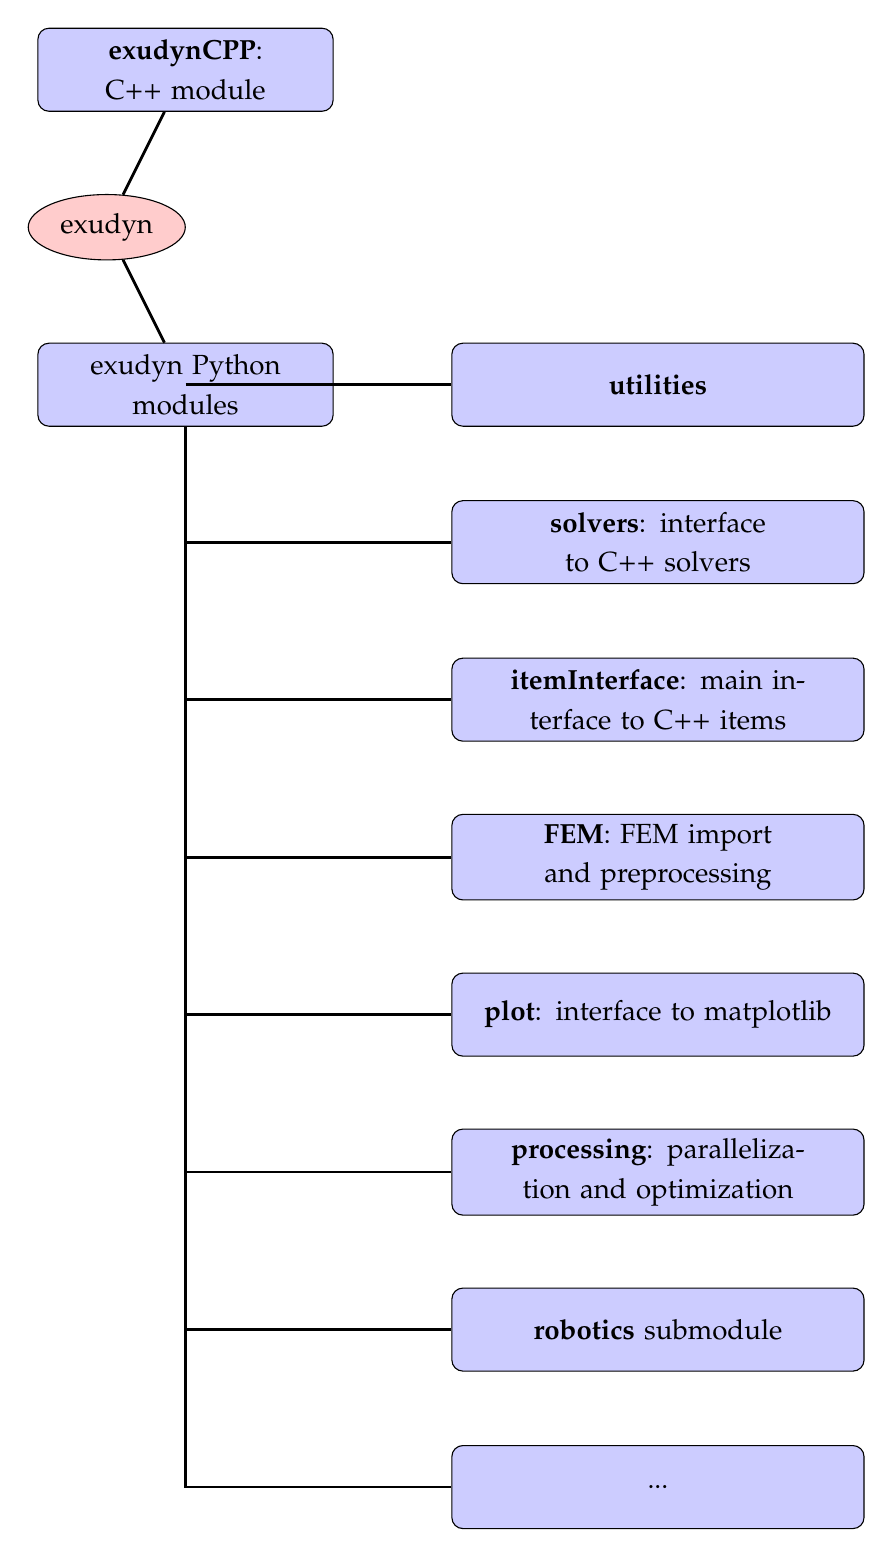
\begin{tikzpicture}[node distance = 2cm, auto]
      % Place nodes
      \node [cloud] (exu) {exudyn};
      \node [wideblock, above of=exu, xshift = 1cm] (exudynCPP) {\mybold{exudynCPP}: C++ module};
      \node [wideblock, below of=exu, xshift = 1cm] (exudynPython) {exudyn Python modules};
      \node [wideblock, right of=exudynPython, node distance=6cm, text width=5cm] (utilities) {\mybold{utilities}};
      \node [wideblock, below of=utilities, text width=5cm] (solvers) {\mybold{solvers}: interface to C++ solvers};
      \node [wideblock, below of=solvers, text width=5cm] (itemInterface) {\mybold{itemInterface}: main interface to C++ items};
      \node [wideblock, below of=itemInterface, text width=5cm] (FEM) {\mybold{FEM}: FEM import and preprocessing};
      \node [wideblock, below of=FEM, text width=5cm] (plot) {\mybold{plot}: interface to matplotlib};
      \node [wideblock, below of=plot, text width=5cm] (processing) {\mybold{processing}: parallelization and optimization};
      \node [wideblock, below of=processing, text width=5cm] (robotics) {\mybold{robotics} submodule};
      \node [wideblock, below of=robotics, text width=5cm] (etc) {...};

      % Draw edges
      \path [line] (exu) -- (exudynCPP);
      \path [line] (exu) -- (exudynPython);

      \path [line] (exudynPython) |- (itemInterface);
      \path [line] (exudynPython) |- (solvers);
      \path [line] (exudynPython) |- (utilities);
      \path [line] (exudynPython) |- (FEM);
      \path [line] (exudynPython) |- (plot);
      \path [line] (exudynPython) |- (processing);
      \path [line] (exudynPython) |- (robotics);
      \path [line] (exudynPython) |- (etc);
  \end{tikzpicture}
  \caption{Overview of exudyn C++ and Python modules.}
  \label{fig_exudyn_CandPython}
\end{figure}

\mysubsubsectionlabel{Overview of modules}{sec:overview:overviewmodules}
Currently, the \codeName\ module structure is split into a C++ core part and a set of 
Python parts, see \fig{fig_exudyn_CandPython}.
\bi
  \item \mybold{C++ parts}, see \fig{fig_exudyn_CPP} and \fig{fig_system_overview}:
  \bi
    \item[--] \texttt{exudyn}:
    on this level, there are just very few functions: \texttt{SystemContainer()}, \texttt{StartRenderer()}, \texttt{StopRenderer()}, \texttt{GetVersionString()}, \texttt{SolveStatic(...)}, \texttt{SolveDynamic(...)}, ... as well as system and user variable dictionaries \texttt{exudyn.variables} and \texttt{exudyn.sys}
    \item[--] \texttt{SystemContainer}: contains the systems (most important), solvers (static, dynamics, ...), visualization settings
    \item[--] \texttt{mbs}: \acf{mbs} created with \texttt{mbs = SC.AddSystem()}, this structure contains everything that defines a solvable multibody system; a large set of nodes, objects, markers, 
    loads can added to the system, see \refSection{sec:item:reference:manual};
    \item[--] \texttt{mbs.systemData}: contains the initial, current, visualization, ... states of the system and holds the items, see \fig{fig_system_overview}
  \ei
  \item \mybold{Python parts} (this list is continuously extended, see \refSection{sec:pythonUtilityFunctions}), sorted by importance:
  \bi
    \item[--] \texttt{exudyn.utilities}: constains helper classes in Python and includes \codeName\ modules \texttt{basicUtilities}, \texttt{rigidBodyUtilities}, \texttt{graphicsDataUtilities}, and \texttt{itemInterface}, which is recommended to be loaded at beginning of your model file
    \item[--] \texttt{exudyn.itemInterface}: contains the interface, which transfers Python classes (e.g., of a NodePoint) to dictionaries that can be understood by the C++ module
    \item[--] \texttt{exudyn.basicUtilities}: contains basic helper classes, without importing numpy
    \item[--] \texttt{exudyn.rigidBodyUtilities}: contains important helper classes for creation of rigid body inertia, rigid bodies, and rigid body joints; includes helper functions for rotation parameterization, rotation matrices, homogeneous transformations, etc.
    \item[--] \texttt{exudyn.graphicsDataUtilities}: provides some basic drawing utilities, definition of colors and basic drawing objects (including \acs{STL} import); rotation/translation of graphicsData objects
    \item[--] \texttt{exudyn.plot}: contains PlotSensor(...), a very versatile interface to matplotlib and other valuable helper functions
    \item[--] \texttt{exudyn.processing}: methods for optimization, parameter variation, sensitivity analysis, etc.
    \item[--] \texttt{exudyn.FEM}: everything related to finite element import and creation of model order reduction flexible bodies
    \item[--] \texttt{exudyn.robotics}: submodule containing several helper modules related to manipulators (\texttt{robotics}, \texttt{robotics.models}), mobile robots (\texttt{robotics.mobile}), trajectory generation (\texttt{robotics.motion}), etc.
    \item[--] \texttt{exudyn.beams}: helper functions for creation of beams along straight lines and curves, sliding joints, etc.
    \item[--] \texttt{exudyn.interactive}: helper classes to create interactive models (e.g. for teaching or demos)
    \item[--] \texttt{exudyn.physics}: containing helper functions, which are physics related such as friction
    \item[--] \texttt{exudyn.signalProcessing}: filters, FFT, etc.; interfaces to scipy and numpy methods
    \item[--] \texttt{exudyn.solver}: functions imported when loading \texttt{exudyn}, containing main solvers
  \ei
\ei
%
%++++++++++++++++++++++++++++++++++++++++++++++++++++++++++++++++++++++++
\onlyRST{

.. _fig-exudyn-cpp:
.. figure:: docs/theDoc/figures/overviewExudynCppModule.png
   :width: 500

   Overview on Exudyn C++ module

}
\begin{figure}
  \centering
  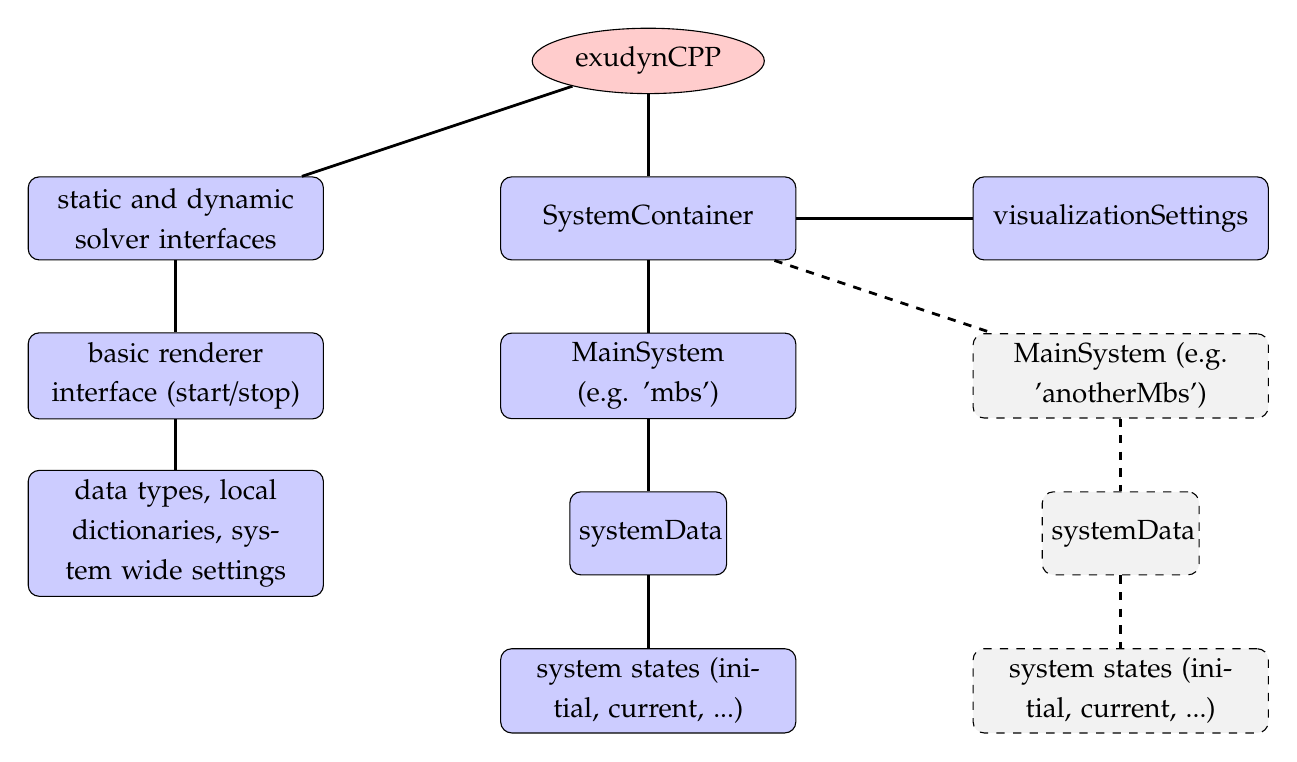
\begin{tikzpicture}[node distance = 2cm, auto]
      % Place nodes
      \node [cloud] (exu) {exudynCPP};
      \node [wideblock, below of=exu] (systemContainer) {SystemContainer};
      \node [wideblock, below of=systemContainer] (system) {MainSystem (e.g. 'mbs')};
      \node [wideblock, right of=systemContainer,  node distance=6cm] (visualizationSettings) {visualizationSettings};
      \node [block, below of=system] (systemData) {systemData};
      \node [wideblock, below of=systemData] (systemStates) {system states (initial, current, ...)};
      \node [wideblock, left of=systemContainer, node distance=6cm] (solver) {static and dynamic solver interfaces};
      \node [wideblock, below of=solver] (renderer) {basic renderer interface (start/stop)};
      \node [wideblock, below of=renderer] (misc) {data types, local dictionaries, system wide settings};
      
      \node [wideblock, dashed, fill=gray!10, right of=system,  node distance=6cm] (anotherSystem) {MainSystem (e.g. 'anotherMbs')};
      \node [block, dashed, fill=gray!10, below of=anotherSystem] (anotherSystemData) {systemData};
      \node [wideblock, dashed, fill=gray!10, below of=anotherSystemData] (anotherSystemStates) {system states 
      (initial, current, ...)};

      %\node [cloud, right of=exu] (itemInterface) {itemInterface.py};
      %\node [cloud, right of=itemInterface] (exudynUtilities) {exudynUtilities.py};

      % Draw edges
      \path [line] (exu) -- (systemContainer);
      \path [line] (systemContainer) -- (system);
      \path [line] (systemContainer) -- (visualizationSettings);
      \path [line] (system) -- (systemData);
      \path [line] (systemData) -- (systemStates);
      \path [line] (exu) -- (solver);
      \path [line] (solver) -- (renderer);
      \path [line] (renderer) -- (misc);

      \path [line, dashed] (systemContainer) -- (anotherSystem);
      \path [line, dashed] (anotherSystem) -- (anotherSystemData);
      \path [line, dashed] (anotherSystemData) -- (anotherSystemStates);
  \end{tikzpicture}
  \caption{Overview of exudyn C++ module.}
  \label{fig_exudyn_CPP}
\end{figure}
%++++++++++++++++++++++++++++++++++++++++++++++++++++++++++++++++++++++++

\onlyRST{

.. _fig-system-overview:
.. figure:: docs/theDoc/figures/overviewSystemData.png
   :width: 550

   Overview of systemData

SystemData connects items, states and stores the \acs{LTG}. Note that access to items is provided via functions in \texttt{MainSystem}.
}
%++++++++++++++++++++++++++++++++++++++++++++++++++++++++++++++++++++++++
\begin{figure}
  \centering
  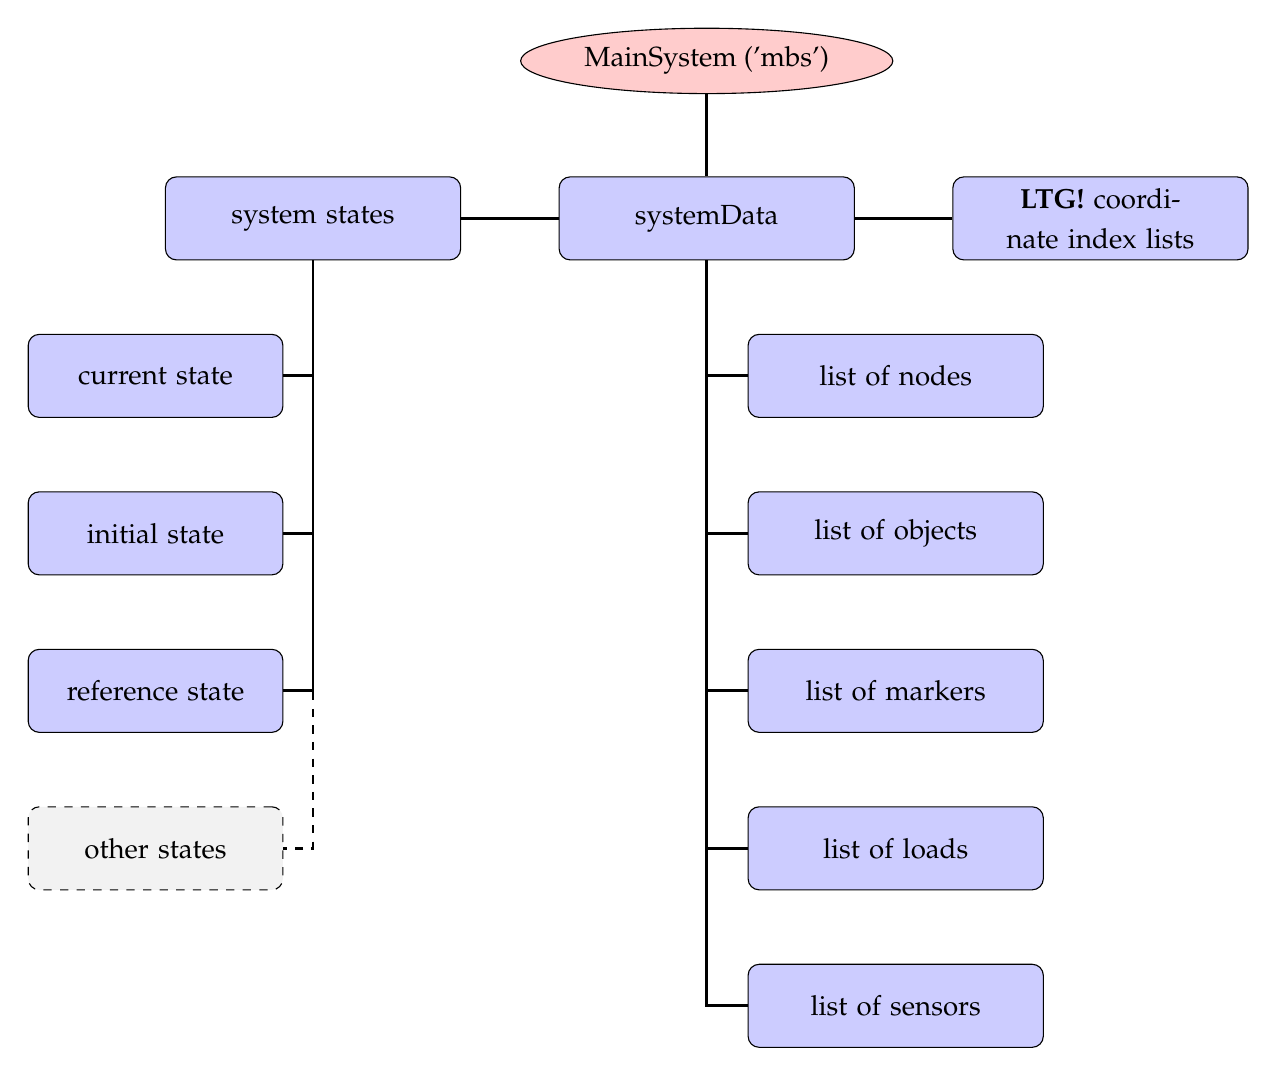
\begin{tikzpicture}[node distance = 2cm, auto]
      % 
      \node [cloud] (system) {MainSystem ('mbs')};
      \node [wideblock, below of=system] (systemData) {systemData};
      \node [wideblock, left of=systemData, node distance=5cm] (systemStates) {system states};
      \node [wideblock, text width=3cm, below of=systemStates, xshift=-2cm] (current) {current state};
      \node [wideblock, text width=3cm, below of=current] (initial) {initial state};
      \node [wideblock, text width=3cm, below of=initial] (reference) {reference state};
      \node [wideblock, text width=3cm, dashed, fill=gray!10, below of=reference] (otherStates) {other states};
%
      \node [wideblock, right of=systemData, node distance=5cm] (ltg) {\acs{LTG} coordinate index lists};
%
      \node [wideblock, below of=systemData, xshift=2.4cm] (nodes) {list of nodes};
      \node [wideblock, below of=nodes] (objects) {list of objects};
      \node [wideblock, below of=objects] (markers) {list of markers};
      \node [wideblock, below of=markers] (loads) {list of loads};
      \node [wideblock, below of=loads] (sensors) {list of sensors};
%
      % Draw edges
      \path [line] (system) -- (systemData);
      \path [line] (systemData) -- (systemStates);
      \path [line] (systemStates) |- (current);
      \path [line] (systemStates) |- (initial);
      \path [line] (systemStates) |- (reference);
      \path [line, dashed] (systemStates) |- (otherStates);
%
      \path [line] (systemData) -- (ltg);
%
      \path [line] (systemData) |- (nodes);
      \path [line] (systemData) |- (objects);
      \path [line] (systemData) |- (markers);
      \path [line] (systemData) |- (loads);
      \path [line] (systemData) |- (sensors);
%
  \end{tikzpicture}
  \caption{Overview of systemData, which connects items, states and stores the \acs{LTG}. Note that access to items is provided via functions in \texttt{MainSystem}.}
  \label{fig_system_overview}

\end{figure}
%++++++++++++++++++++++++++++++++++++++++++++++++++++++++++++++++++++++++


\mysubsubsectionlabel{Conventions: items, indexes, coordinates}{sec:overview:conventionsitems}
In this documentation, we will use the term \mybold{item} to identify nodes, objects, markers, loads and sensors: \vspace{6pt}

  item $\in$ \{node, object, marker, load, sensor\} \vspace{12pt}

\noindent \mybold{Indexes: arrays and vectors starting with 0:} \vspace{6pt}\\
As known from Python, all \mybold{indexes} of arrays, vectors, matrices, ...\ are starting with 0. This means that the first component of the vector \texttt{v=[1,2,3]} is accessed with \texttt{v[0]} in Python (and also in the C++ part of \codeName ). The range is usually defined as \texttt{range(0,3)}, in which '3' marks the index after the last valid component of an array or vector.
\ignoreRST{\vspace{12pt}\\}
%
\mybold{Dimensionality of objects and vectors:} \ignoreRST{\vspace{6pt}}\\ 
\ac{2D} vs.\ \ac{3D}
\ignoreRST{\vspace{6pt}\\}
As a convention, quantities in \codeName\ are 3D, such as nodes, objects, markers, loads, measured quantities, etc. 
For that reason, we denote planar nodes, objects, etc.\ with the suffix 2D, but 3D objects do not get this suffix\footnote{There are some rare exceptions, such as Beam3D as the pure beam may easily lead to name space conflicts in Python}.

Output and input to objects, markers, loads, etc.\ is usually given by 3D vectors (or matrices), such as (local) position, force, torque, rotation, etc. However, initial and reference values for nodes depend on their dimensionality.
As an example, consider a \texttt{NodePoint2D}:
\bi
  \item \texttt{referenceCoordinates} is a 2D vector (but could be any dimension in general nodes)
  \item measuring the current position of \texttt{NodePoint2D} gives a 3D vector
  \item when attaching a \texttt{MarkerNodePosition} and a \texttt{LoadForceVector}, the force will be still a 3D vector
\ei
Furthermore, the local position in 2D objects is provided by a 3D vector. Usually, the dimensionality is given in the reference manual. User errors in the dimensionality will be usually detected either by the Python interface (i.e., at the time the item is created) or by the system-preprocessor

\mysubsectionlabel{Items: Nodes, Objects, Loads, Markers, Sensors, ...}{sec:overview:items}
%
In this section, the most important part of \codeName\ are provided. An overview of the interaction of the items is given in \fig{fig_items_interaction}

%++++++++++++++++++++++++++++++++++++++++++++++++++++++++++++++++++++++++
\onlyRST{

.. _fig-items-interaction:
.. figure:: docs/theDoc/figures/itemsMultibodySystem.png
   :width: 500

   Interaction of items in a multibody system

Note that both, bodies and connectors (including constraints) are -- computational -- objects. The arrows indicate, that, e.g., object 1 has node 1 and node 2 (indexes) and that marker 0 is attached to object 0, while load 0 uses marker 0 to apply the load. Sensors could additionally be attached to certain items.

}
%++++++++++++++++++++++++++++++++++++++++++++++++++++++++++++++++++++++++
\begin{figure}
  \centering
  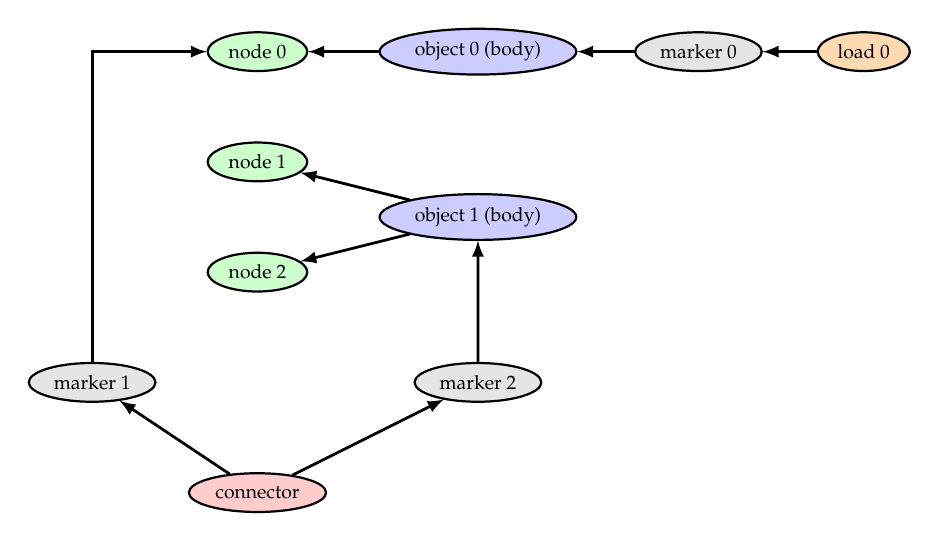
\begin{tikzpicture}[node distance = 2cm, auto, thick,scale=0.7, every node/.style={scale=0.7}]
      % Place nodes
      \node [nodeBlock] (node0) {node 0};
      \node [nodeBlock, below of=node0, node distance=2cm] (node1) {node 1};
      \node [nodeBlock, below of=node1, node distance=2cm] (node2) {node 2};

      \node [objectBlock, right of=node0] (object0) {object 0 (body)};
      \node [objectBlock, right of=node1, yshift = -1cm] (object1) {object 1 (body)};
      
      \node [markerBlock, right of=object0] (marker0) {marker 0};
      \node [loadBlock, right of=marker0, node distance=3cm] (load0) {load 0};
      
      \node [markerBlock, left of=node2, yshift = -2cm, xshift = 1cm] (marker1) {marker 1};
      \node [markerBlock, right of=node2, yshift = -2cm] (marker2) {marker 2};

      \node [connectorBlock, below of=node2] (connector) {connector};


      \path [arrow] (object0) -- (node0);
      \path [arrow] (marker0) -- (object0);
      \path [arrow] (load0) -- (marker0);
      \path [arrow] (object1) -- (node1);
      \path [arrow] (object1) -- (node2);
      \path [arrow] (marker1) |- (node0);
      \path [arrow] (marker2) -- (object1);
      \path [arrow] (connector) -- (marker1);
      \path [arrow] (connector) -- (marker2);
      %\path [line] (systemData) |- (objects);
      %\path [line] (systemData) |- (markers);
      %\path [line] (systemData) |- (loads);

  \end{tikzpicture}
  \caption{Interaction of items in a multibody system. 
Note that both, bodies and connectors (including constraints) are -- computational -- objects.
The arrows indicate, that, e.g., object 1 has node 1 and node 2 (indexes) and that marker 0 is attached to object 0, while load 0 uses marker 0 to apply the load. Sensors could additionally be attached to certain items.}
  \label{fig_items_interaction}

\end{figure}
%++++++++++++++++++++++++++++++++++++++++++++++++++++++++++++++++++++++++

\mysubsubsection{Nodes}
Nodes provide the coordinates (and the degrees of freedom) to the system. They have no mass, stiffness or whatsoever assigned.
Without nodes, the system has no unknown coordinates.
Adding a node provides (for the system unknown) coordinates. In addition we also need equations for every nodal coordinate -- otherwise the system cannot be computed (NOTE: this is currently not checked by the preprocessor).

\mysubsubsection{Objects}
Objects are 'computational objects' and they provide equations to your system. Objects often provide derivatives and have measurable quantities (e.g. displacement) and they provide access, which can be used to apply, e.g., forces. Some of this functionality is only available in C++, but not in Python.

Objects can be a:
\bi
  \item general object (e.g.\ a controller, user defined object, ...; no example yet)
  \item body: has a mass or mass distribution; markers can be placed on bodies; loads can be applied; constraints can be attached via markers; bodies can be:
  \bi
    \item[--] ground object: has no nodes
    \item[--] simple body: has one node (e.g. mass point, rigid body)
    \item[--] finite element and more complicated body (e.g. FFRF-object): has more than one node
  \ei
  \item connector: uses markers to connect nodes and/or bodies; adds additional terms to system equations either based on stiffness/damping or with constraints (and Lagrange multipliers). Possible connectors:
  \bi
    \item[--] algebraic constraint (e.g. constrain two coordinates: $q_1 = q_2$)
    \item[--] classical joint
    \item[--] spring-damper or penalty constraint
  \ei
\ei

\mysubsubsection{Markers}
Markers are interfaces between objects/nodes and constraints/loads.
A constraint (which is also an object) or load cannot act directly on a node or object without a marker.
As a benefit, the constraint or load does not need to know whether it is applied, e.g., to a node or to a local position of a body.

Typical situations are:
\bi
  \item Node -- Marker -- Load
  \item Node -- Marker -- Constraint (object)
  \item Body(object) -- Marker -- Load
  \item Body1 -- Marker1 -- Joint(object) -- Marker2 -- Body2
\ei

\mysubsubsection{Loads}
Loads are used to apply forces and torques to the system. The load values are static values. However, you can use Python functionality to modify loads either by linearly increasing them during static computation or by using the 'mbs.SetPreStepUserFunction(...)' structure in order to modify loads in every integration step depending on time or on measured quantities (thus, creating a controller).

\mysubsubsection{Sensors}
Sensors are only used to measure output variables (values) in order to simpler generate the requested output quantities.
They have a very weak influence on the system, because they are only evaluated after certain solver steps as requested by the user.

\mysubsubsectionlabel{Reference coordinates and displacements}{sec:overview:items:coordinates}
Nodes usually have separated reference and initial quantities. Here, 
\texttt{referenceCoordinates} are the coordinates for which the system is defined upon creation. Reference coordinates are needed, e.g., for definition of joints and for the reference configuration of finite elements. In many cases it marks the undeformed configuration (e.g., with finite elements), but not, e.g., for \texttt{ObjectConnectorSpringDamper}, which has its own reference length. 

Initial displacement (or rotation) values are provided separately, in order to start a system from a configuration different from the reference configuration.
As an example, the initial configuration of a \texttt{NodePoint} is given by \texttt{referenceCoordinates + initialCoordinates}, while the initial state of a dynamic system additionally needs \texttt{initialVelocities}.

\mysubsectionlabel{Mapping between local and global coordinate indices}{sec:overview:ltgmapping}
%
The \ac{LTG}-index-mappings\footnote{local-to-global coordinate index mappings containing transformation from local object coordinate indices to global (system) coordinate indices; this is different for \mybold{coordinate transformations}!} between local coordinate \mybold{indices}, on node or object level, and global (=system) coordinate \mybold{indices} follows the following rules:
\bi
\item \ac{LTG}-index-mappings are computed during \texttt{mbs.Assemble()} and are not available before.
\item Nodes own a global index which relates the local coordinates to global (system) coordinate. E.g., for a \ac{ODE2} node with node number \texttt{i}, this index can be obtained via the function \texttt{mbs.GetNodeODE2Index(i)}.
\item The order of global coordinates is simply following the node numbering. If we add three nodes \texttt{NodePoint}, the system will contain 9 coordinates, where the first triple (starting index 0) belongs to node 0, the second triple (starting index 3) belongs to node 1 and the third triple (starting index 6) belongs to node 2. After \texttt{mbs.Assemble()}, you can access the system coordinates via \texttt{mbs.systemData.GetODE2Coordinates()}, which returns a numpy array with 9 coordinates, containing the initial values provided in \texttt{NodePoint} (default: zero).
\item Objects have their own \ac{LTG}-index-mappings for their respective coordinate types. The \ac{ODE2} coordinates of an object \texttt{j} can be retrieved via \texttt{mbs.systemData.GetObjectLTGODE2(j)}. For a body, these are the global \ac{ODE2} coordinates representing the body; for a connector, these are the coordinates to which the connector is linked (usually coordinates of two bodies); for a ground object, the \ac{LTG}-index-mapping is empty; see also \refSection{sec:systemData:ObjectLTG}.
\item Constraints create algebraic variables (Lagrange multipliers) automatically. For a constraint with object number \texttt{k}, the global index to algebraic variables (of \ac{AE}-type) can be accessed via \texttt{mbs.systemData.GetObjectLTGAE(k)}.
\ei

\mysubsectionlabel{Exudyn Basics}{sec:overview:basics}
This section will show:
\bi
  \item Interaction with the \codeName\ module
  \item Simulation settings
  \item Visualization settings
  \item Generating output and results
  \item Graphics pipeline
  \item Generating animations
\ei

\mysubsubsectionlabel{Interaction with the \codeName\ module}{sec:overview:basics:interactionmodule}
It is important that the \codeName\ module is basically a state machine, where you create items on the C++ side using the Python interface. This helps you to easily set up models using many other Python modules (numpy, sympy, matplotlib, ...) while the computation will be performed in the end on the C++ side in a very efficient manner. 
\vspace{12pt}\\
\mybold{Where do objects live?}\vspace{6pt}\\
%(where do objects live? state machine; graphics interaction)
Whenever a system container is created with \texttt{SC = exu.SystemContainer()}, the structure \texttt{SC} becomes a variable in the Python interpreter, but it is managed inside the C++ code and it can be modified via the Python interface.
Usually, the system container will hold at least one system, usually called \texttt{mbs}.
Commands such as \texttt{mbs.AddNode(...)} add objects to the system \texttt{mbs}. 
The system will be prepared for simulation by \texttt{mbs.Assemble()} and can be solved (e.g., using \texttt{exu.SolveDynamic(...)}) and evaluated hereafter using the results files.
Using \texttt{mbs.Reset()} will clear the system and allows to set up a new system. Items can be modified (\texttt{ModifyObject(...)}) after first initialization, even during simulation.
%

\mysubsubsectionlabel{Simulation settings}{sec:overview:basics:simulationsettings}
The simulation settings consists of a couple of substructures, e.g., for \texttt{solutionSettings}, \texttt{staticSolver}, \texttt{timeIntegration} as well as a couple of general options -- for details see \refSection{sec:SolutionSettings} and \refSection{sec:SimulationSettings}.

Simulation settings are needed for every solver. They contain solver-specific parameters (e.g., the way how load steps are applied), information on how solution files are written, and very specific control parameters, e.g., for the Newton solver. 

\noindent The simulation settings structure is created with 
\pythonstyle\begin{lstlisting}
  simulationSettings = exu.SimulationSettings()
\end{lstlisting}
%
Hereafter, values of the structure can be modified, e.g.,
\pythonstyle\begin{lstlisting}
  tEnd = 10 #10 seconds of simulation time:
  h = 0.01  #step size (gives 1000 steps)
  simulationSettings.timeIntegration.endTime = tEnd
  #steps for time integration must be integer:
  simulationSettings.timeIntegration.numberOfSteps = int(tEnd/h)
  #assigns a new tolerance for Newton's method:
  simulationSettings.timeIntegration.newton.relativeTolerance = 1e-9 
  #write some output while the solver is active (SLOWER):
  simulationSettings.timeIntegration.verboseMode = 2                 
  #write solution every 0.1 seconds:
  simulationSettings.solutionSettings.solutionWritePeriod = 0.1      
  #use sparse matrix storage and solver (package Eigen):
  simulationSettings.linearSolverType = exu.LinearSolverType.EigenSparse 
\end{lstlisting}

\mysubsubsection{Generating output and results}
%
The solvers provide a number of options in \texttt{solutionSettings} to generate a solution file. As a default, exporting the solution of all system coordinates (on position, velocity, ... level) to the solution file is activated with a writing period of 0.01 seconds.

\noindent Typical output settings are:
\pythonstyle\begin{lstlisting}
  #create a new simulationSettings structure:
  simulationSettings = exu.SimulationSettings()
  
  #activate writing to solution file:
  simulationSettings.solutionSettings.writeSolutionToFile = True
  #write results every 1ms:
  simulationSettings.solutionSettings.solutionWritePeriod = 0.001
  
  #assign new filename to solution file
  simulationSettings.solutionSettings.coordinatesSolutionFileName= "myOutput.txt"

  #do not export certain coordinates:
  simulationSettings.solutionSettings.exportDataCoordinates = False
\end{lstlisting}

Furthermore, you can use sensors to record particular information, e.g., the displacement of a body's local
position, forces or joint data. For viewing sensor results, use the \texttt{PlotSensor} function of the 
\texttt{exudyn.plot} tool, see the rigid body and joints tutorial.


\mysubsubsectionlabel{Visualization settings dialog}{sec:overview:basics:visualizationsettings}
%
Visualization settings are used for user interaction with the model. E.g., the nodes, markers, loads, etc., can be visualized for every model. There are default values, e.g., for the size of nodes, which may be inappropriate for your model. Therefore, you can adjust those parameters. In some cases, huge models require simpler graphics representation, in order not to slow down performance -- e.g., the number of faces to represent a cylinder should be small if there are 10000s of cylinders drawn. Even computation performance can be slowed down, if visualization takes lots of CPU power. However, visualization is performed in a separate thread, which usually does not influence the computation exhaustively.

Details on visualization settings and its substructures are provided in \refSection{sec:VSettingsGeneral} -- \refSection{sec:VisualizationSettings}. These settings may also be edited by pressing 'V' in the active render window (does not work, if there is no active render loop using, e.g., \texttt{SC.WaitForRenderEngineStopFlag()} or 
\texttt{mbs.WaitForUserToContinue()} ).
The visualization settings dialog is shown exemplarily in \fig{fig_visualizationSettings}.
Note that this dialog is automatically created and uses Python's \texttt{tkinter}, which is lightweight, but not very well suited if display scalings are large (e.g., on high resolution laptop screens). If working with Spyder, it is recommended to restart Spyder, if display scaling is changed, in order to adjust scaling not only for Spyder but also for \codeName\ .

The appearance of visualization settings dialogs may be adjusted by directly modifying \texttt{exudyn.GUI} variables (this may change in the future). For example write in your code before opening the render window\footnote{treeEdit and treeview both mean the settings dialog currently used for visualization settings and partially for right-mouse-click}:
\pythonstyle\begin{lstlisting}
  import exudyn.GUI
  exudyn.GUI.dialogDefaultWidth             #unscaled width of, e.g., right-mouse-button dialog
  exudyn.GUI.treeEditDefaultWidth = 800
  exudyn.GUI.treeEditDefaultHeight = 600
  exudyn.GUI.treeEditMaxInitialHeight = 600 #otherwise height is increased for larger screens
  exudyn.GUI.treeEditOpenItems = ['general','contact'] #these tree items are opened each time the dialog is opened
  #
  exudyn.GUI.treeviewDefaultFontSize        #this is the base font size of the dialog (also right-mouse-button dialog)
  exudyn.GUI.useRenderWindowDisplayScaling  #if True, the scaling will follow the current scaling of the render window; if False, it will use the \texttt{tkinter} internal scaling, which uses the main screen where the dialog is created (which won't scale well, if the window is moved to another screen).
  #
  exudyn.GUI.textHeightFactor = 1.45        #this factor is used to increase height of lines in tree view as compared to font size
\end{lstlisting}
%
\onlyRST{

.. _fig-visualizationsettings:
.. figure:: docs/theDoc/figures/visualizationSettings.png
   :width: 700

   View of visualization settings

Note: Press 'V' in render window to open dialog.
}
\ignoreRST{
\begin{figure}[tbhp]%
\begin{center}
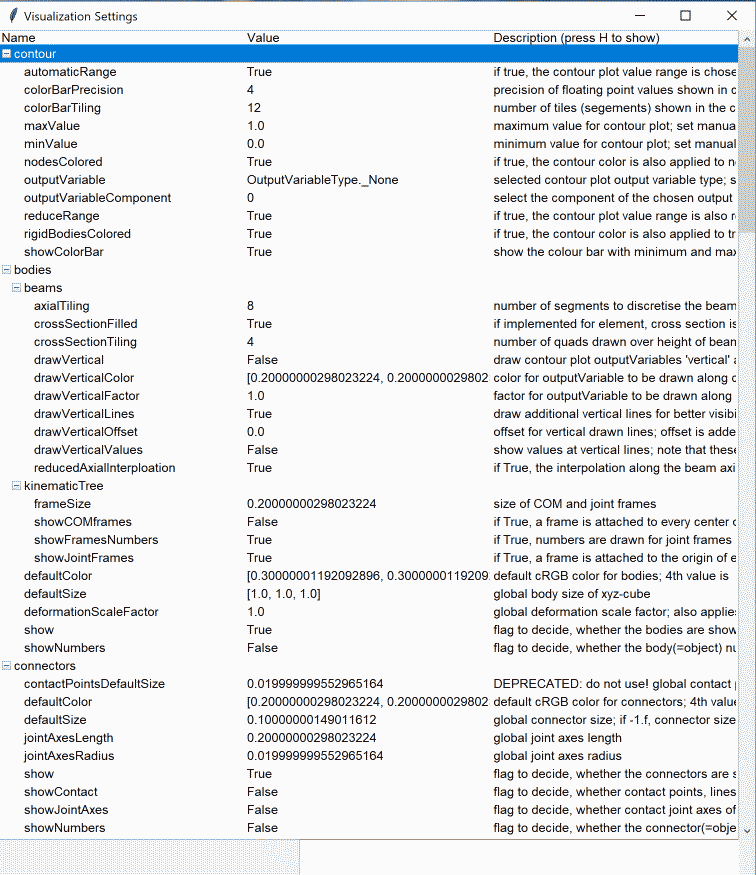
\includegraphics[width=0.8\columnwidth]{figures/visualizationSettings}
\end{center}
\caption{View of visualization settings (as of \codeName\ 1.5.51.dev1) (press 'V' in render window to open dialog)}%
\label{fig_visualizationSettings}%
\end{figure}
}

\noindent
The visualization settings structure can be accessed in the system container \texttt{SC} (access per reference, no copying!), accessing every value or structure directly, e.g.,
\pythonstyle\begin{lstlisting}
  SC.visualizationSettings.nodes.defaultSize = 0.001      #draw nodes very small

  #change openGL parameters; current values can be obtained from SC.GetRenderState()
  #change zoom factor:
  SC.visualizationSettings.openGL.initialZoom = 0.2       
  #set the center point of the scene (can be attached to moving object):
  SC.visualizationSettings.openGL.initialCenterPoint = [0.192, -0.0039,-0.075]

  #turn of auto-fit:
  SC.visualizationSettings.general.autoFitScene = False

  #change smoothness of a cylinder:
  SC.visualizationSettings.general.cylinderTiling = 100
  
  #make round objects flat:
  SC.visualizationSettings.openGL.shadeModelSmooth = False

  #turn on coloured plot, using y-component of displacements:
  SC.visualizationSettings.contour.outputVariable = exu.OutputVariableType.Displacement
  SC.visualizationSettings.contour.outputVariableComponent = 1 #0=x, 1=y, 2=z
\end{lstlisting}

\mysubsubsectionlabel{Renderer and 3D graphics}{sec:overview:basics:renderer}
A 3D renderer is attached to the simulation. Visualization is started with  \texttt{exu.StartRenderer()}, see the examples and tutorials.
The renderer uses an OpenGL window of a library called GLFW, which is platform-independent. 
The renderer is set up in a minimalistic way, just to ensure that you can check that the modeling is correct. There is no way to contruct models with the renderer. Try to avoid huge number of triangles in STL files or by creating large number of complex objects, such as spheres or cylinders.

\noindent There are some main features in the renderer, using keyboard and mouse:
\bi
  \item press key H to show help in renderer
  \item move model by pressing left mouse button and drag
  \item rotate model by pressing right mouse button and drag
  \item change visibility (wire frame, solid, transparent, ...) by pressing T
  \item zoom all: key A
  \item open visualization dialog: key V
  \item show item number: click on graphics element with left mouse button
  \item show item dictionary: click on graphics element with right mouse button  
  \item ... (see \refSection{sec:VSettingsGeneral}ff.)
\ei
%
Depending on your model (size, place, ...), you may need to adjust the following \texttt{openGL} parameters in \texttt{visualizationSettings}:
\bi
  \item light and light position 
  \item shadow (turned off by using 0; turned on by using, e.g., a value of 0.3) and shadow polygon offset; shadow slows down graphics performance by a factor of 2-3, depending on your graphics card
  \item visibility of nodes, markers, etc. in according bodies, nodes, markers, ..., \texttt{visualizationSettings}
  \item move camera with a selected marker: adjust \texttt{trackMarker} in \texttt{visualizationSettings.interactive}
  \item ... (see \refSection{sec:VSettingsGeneral}ff.)
\ei


\mysubsubsectionlabel{Graphics pipeline}{sec:overview:basics:graphicspipeline}
%deprecated, since there are user functions!: The user cannot interact with the visualization part for now.
There are basically two loops during simulation, which feed the graphics pipeline.
The solver runs a loop:
\bi
  \item compute step (or set up initial values)
  \item finish computation step; results are in current state
  \item copy current state to visualization state (thread safe)
  \item signal graphics pipeline that new visualization data is available
  \item the renderer may update the visualization depending on \texttt{graphicsUpdateInterval} in \\ \texttt{visualizationSettings.general}
\ei
The openGL graphics thread (=separate thread) runs the following loop:
\bi
  \item render openGL scene with a given graphicsData structure (containing lines, faces, text, ...)
  \item go idle for some milliseconds
  \item check if openGL rendering needs an update (e.g. due to user interaction)
  \item[] $\ra$ if update is needed, the visualization of all items is updated -- stored in a graphicsData structure)
  \item check if new visualization data is available and the time since last update is larger than a presribed value, the graphicsData structure is updated with the new visualization state
\ei

\mysubsubsectionlabel{Storing the model view}{sec:overview:basics:storingmodelview}
There is a simple way to store the current view (zoom, centerpoint, orientation, etc.) by using \texttt{SC.GetRenderState()} and \texttt{SC.SetRenderState()},
see also \refSection{sec:renderState}.
%
A simple way is to reload the stored render state (model view) after simulating your model once at the end of the simulation\footnote{
note that \texttt{visualizationSettings.general.autoFitScene} should be set False if you want to use the stored zoom factor}:
\pythonstyle\begin{lstlisting}
  import exudyn as exu
  SC=exu.SystemContainer()
  SC.visualizationSettings.general.autoFitScene = False #prevent from autozoom
  exu.StartRenderer()
  if 'renderState' in exu.sys:
      SC.SetRenderState(exu.sys['renderState']) 
  #+++++++++++++++
  #do simulation here and adjust model view settings with mouse
  #+++++++++++++++

  #store model view for next run:
  StopRenderer() #stores render state in exu.sys['renderState']
\end{lstlisting}
\horizontalRuler \\
%
Alternatively, you can obtain the current model view from the console after a simulation, e.g.,
\pythonstyle\begin{lstlisting}
  In[1] : SC.GetRenderState()
  Out[1]: 
  {'centerPoint': [1.0, 0.0, 0.0],
   'maxSceneSize': 2.0,
   'zoom': 1.0,
   'currentWindowSize': [1024, 768],
   'modelRotation': [[ 0.34202015,  0.        , 0.9396926 ],
                     [-0.60402274,  0.76604444, 0.21984631],
                     [-0.7198463 , -0.6427876 , 0.26200265]])}
\end{lstlisting}
%
which contains the last state of the renderer.
Now copy the output and set this with \texttt{SC.SetRenderState} in your Python code to have a fixed model view in every simulation (\texttt{SC.SetRenderState} AFTER \texttt{exu.StartRenderer()}):
\pythonstyle\begin{lstlisting}
  SC.visualizationSettings.general.autoFitScene = False #prevent from autozoom
  exu.StartRenderer()
  renderState={'centerPoint': [1.0, 0.0, 0.0],
               'maxSceneSize': 2.0,
               'zoom': 1.0,
               'currentWindowSize': [1024, 768],
               'modelRotation':     [[ 0.34202015,  0.        ,  0.9396926 ],
                                    [-0.60402274,  0.76604444,  0.21984631],
                                    [-0.7198463 , -0.6427876 ,  0.26200265]])
  SC.SetRenderState(renderState)
  #.... further code for simulation here
\end{lstlisting}
Note that in the current version of \codeName\ there is more data stored in render state, which is not used in \texttt{SC.SetRenderState},
see also \refSection{sec:renderState}.
\horizontalRuler
%

\mysubsubsection{Graphics user functions via Python}
There are some user functions in order to customize drawing:
\bi
  \item You can assign graphicsData to the visualization to most bodies, such as rigid bodies in order to change the shape. Graphics can also be imported from files (\texttt{GraphicsDataFromSTLfileTxt}) using the established format \ac{STL}\footnote{STereoLithography or Standard Triangle Language; file format available in nearly all CAD systems}.
  \item Some objects, e.g., \texttt{ObjectGenericODE2} or \texttt{ObjectRigidBody}, provide customized a function \texttt{graphicsDataUserFunction}. This user function just returns a list of GraphicsData, see \refSection{sec:graphicsData}. With this function you can change the shape of the body in every step of the computation.
  \item Specifically, the \texttt{graphicsDataUserFunction} in \texttt{ObjectGround} can be used to draw any moving background in the scene.
\ei
Note that all kinds of \texttt{graphicsDataUserFunction}s need to be called from the main (=computation) process as Python functions may not be called from separate threads (GIL). Therefore, the computation thread is interrupted to execute the \texttt{graphicsDataUserFunction} between two time steps, such that the graphics Python user function can be executed. There is a timeout variable for this interruption of the computation with a warning if scenes get too complicated.

\mysubsubsectionlabel{Color, RGBA and alpha-transparency}{sec:overview:basics:colorrgba}
Many functions and objects include color information. In order to allow alpha-transparency, all colors contain a list of 4 RGBA values, all values being in the range [0..1]:
\bi
  \item red (R) channel 
  \item green (G) channel  
  \item blue (B) channel 
  \item alpha (A) value, representing the so-called \mybold{alpha-transparency} (A=0: fully transparent, A=1: solid)
\ei
E.g., red color with no transparency is obtained by the color=[1,0,0,1]. Color predefinitions are found in \texttt{exudynGraphicsDataUtilities.py}, e.g., \texttt{color4red} or \texttt{color4steelblue} as well a list of 16 colors \texttt{color4list}, which is convenient to be used in a loop creating objects.

\mysubsubsectionlabel{Solution viewer}{sec:overview:basics:solutionviewer}
\codeName\ offers a convenient WYSIWYS -- 'What you See is What you Simulate' interface, showing you the computation results during simulation in the render window.
If you are running large models, it may be more convenient to watch results after simulation has been finished.
For this, you can use
\bi
  \item \texttt{interactive.SolutionViewer}, see \refSectionA{sec:interactive:SolutionViewer}
  \item \texttt{interactive.AnimateModes}, lets you view the animation of computed modes, see \refSectionA{sec:interactive:AnimateModes}
\ei
shown exemplary in \fig{fig_solutionViewer}.
\onlyRST{

.. _fig-solutionviewer:
.. figure:: docs/theDoc/figures/solutionViewer.png
   :width: 800

   View of \texttt{SolutionViewer} (as of \codeName\ 1.5.42.dev1)

}
\ignoreRST{
\begin{figure}[tbhp]%
\begin{center}
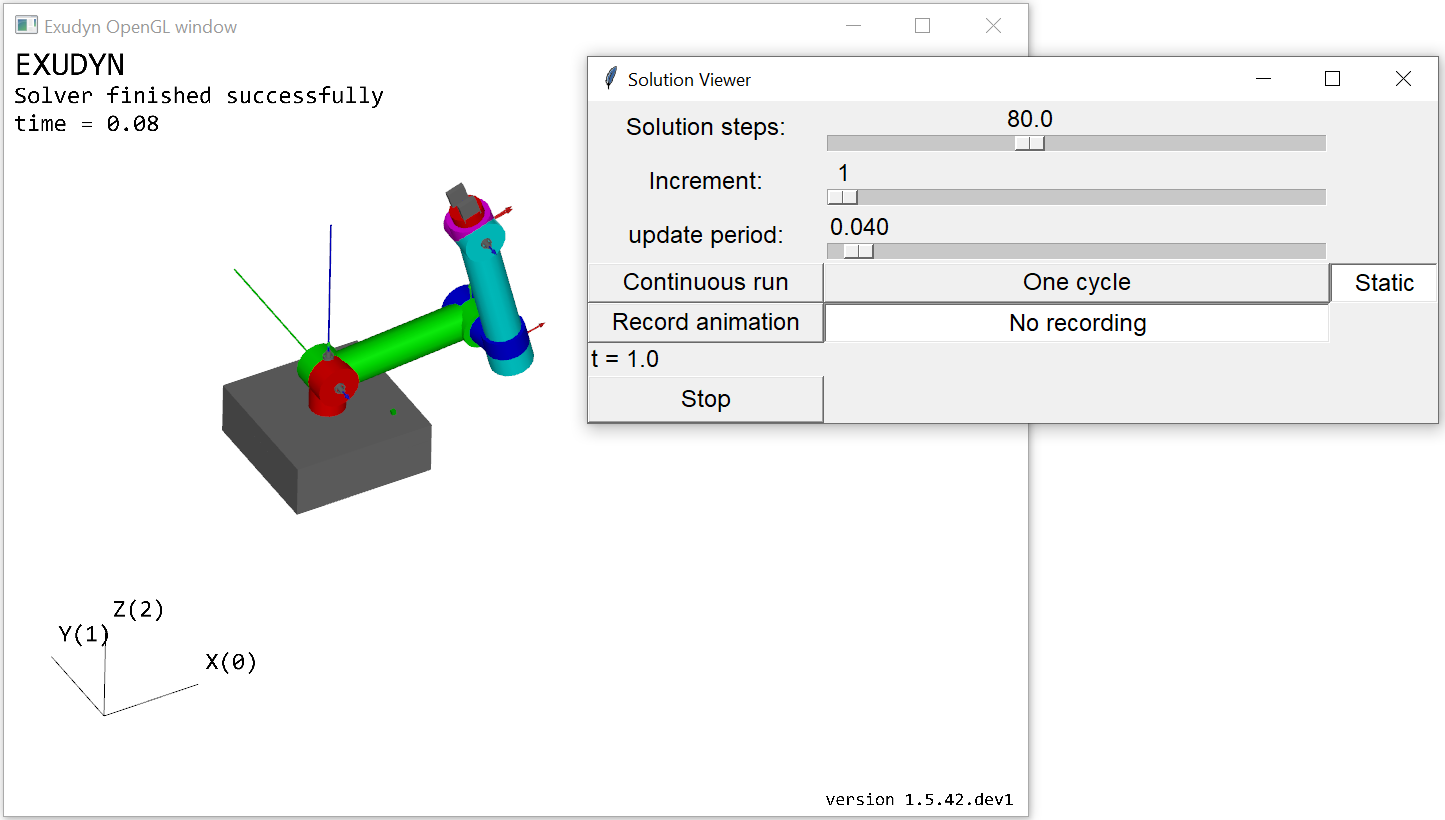
\includegraphics[width=0.98\columnwidth]{figures/solutionViewer}
\end{center}
\caption{View of \texttt{SolutionViewer} (as of \codeName\ 1.5.42.dev1)}%
\label{fig_solutionViewer}%
\end{figure}
}
The \texttt{SolutionViewer} adds a \texttt{tkinter} interactive dialog, which lets you interact with the model, with the following features:
\bi
\item The SolutionViewer represents a 'Player' for the dynamic solution or a series of static solutions, which is available after simulation if \texttt{solutionSettings.writeSolutionToFile = True}
\item The parameter \texttt{solutionSettings.solutionWritePeriod} represents the time period used to store solutions during dynamic computations.
\item As soon as 'Run' is pressed, the player runs (and it may be started automatically as well)
\item In the 'Static' mode, drag the slider 'Solution steps' to view the solution steps
\item In the 'Continuous run' mode, the player runs in an infinite loop
\item In the 'One cycle' mode, the player runs from the current position to the end; this is perfectly suited to record series of images for \mybold{creating animations}, see \refSection{sec:overview:basics:animations} and works together with the visualization settings dialog.
\ei
The solution should be loaded with
\texttt{LoadSolutionFile('coordinatesSolution.txt')}, where 'coordinatesSolution.txt' represents the stored solution file, 
see 
\bi
  \item \texttt{exu.SimulationSettings().solutionSettings.coordinatesSolutionFileName}
\ei
You can call the \texttt{SolutionViewer} either in the model, or at the command line / IPython to load a previous solution (belonging to the same mbs underlying the solution!):
\pythonstyle\begin{lstlisting}
  from exudyn.interactive import SolutionViewer
  sol = LoadSolutionFile('coordinatesSolution.txt')
  SolutionViewer(mbs, sol)
\end{lstlisting}
%
\mybold{Alternatively}, if no solution is provided, \texttt{SolutionViewer} tries to reload the solution of the previous simulation that is referred to from \texttt{mbs.sys$[$simulationSettings$]$}:
\pythonstyle\begin{lstlisting}
  from exudyn.interactive import SolutionViewer
  SolutionViewer(mbs)
\end{lstlisting}
An example for the \texttt{SolutionViewer} is integrated into the \texttt{Examples/} directory, see \texttt{solutionViewerTest.py}. \\
\mybold{Note}: The previous function \texttt{AnimateSolution} in \texttt{exudyn.utilities} allows to directly visualize the stored solution for according stored time frames without \texttt{tkinter} (useful for MacOS).

%+++++++++++++++++++++++++++++++++++++++++++++++++++++++++++++++++
\mysubsubsectionlabel{Generating animations}{sec:overview:basics:animations}
%
In many dynamics simulations, it is very helpful to create animations in order to better understand the motion of bodies. Specifically, the animation can be used to visualize the model much slower or faster than the model is computed.

Animations are created based on a series of images (frames, snapshots) taken during simulation. It is important, that the current view is used to record these images -- this means that the view should not be changed during the recording of images.
To turn on recording of images during solving, set the following flag to a positive value
\bi
  \item \texttt{simulationSettings.solutionSettings.recordImagesInterval = 0.01}
\ei
which means, that after every 0.01 seconds of simulation time, an image of the current view is taken and stored in the directory and filename (without filename ending) specified by 
\bi
  \item \texttt{SC.visualizationSettings.exportImages.saveImageFileName = "myFolder/frame"}
\ei
By default, a consecutive numbering is generated for the image, e.g., 'frame0000.png, frame0001.png,...'. Note that the standard file format PNG with ending '.png' uses compression libraries included in glfw, while the alternative TGA format produces '.tga' files which contain raw image data and therefore can become very large.

To create animation files, an external tool FFMPEG is used to efficiently convert a series of images into an animation.
\onlyRST{$\ra$ see theDoc.pdf !}
\ignoreRST{
In windows, simple DOS batch files can do the job to convert frames given in the local directory to animations, e.g.:
\plainlststyle
\lstinputlisting[breaklines=true, basicstyle=\ttm]{../userTools/makeAnimations/convertToVideo.bat}
After the video has been created, you should delete the single images:
\plainlststyle
\lstinputlisting[breaklines=true, basicstyle=\ttm]{../userTools/makeAnimations/deletePNGimages.bat}
}

%+++++++++++++++++++++++++++++++++++++++++++++++++++++++++++++++++
\mysubsubsectionlabel{Examples, test models and test suite}{sec:overview:basics:examplestestsuite}

The main collection of examples and models is available under
\bi
  \item \texttt{main/pythonDev/Examples}
  \item \texttt{main/pythonDev/TestModels}
\ei
You can use these examples to build up your own realistic models of multibody systems.
Very often, these models show the way which already works. Alternative ways may exist, but
sometimes there are limitations in the underlying C++ code, such that they won't work as you expect.

We would like to note that, even that some examples and test models contain comparison to 
papers of the literature or analytical solutions, there are many models which may not contain real
mechanical values and these models may not be converged in space or time 
(in order to keep running our test suite in less than a minute).

Finally, note that the \texttt{main/pythonDev/TestModels} are often only intended to preserve functionality
in the Python and C++ code (e.g., if global methods are changed), but they should not be misinterpreted as validation of the 
implemented methods. The \texttt{TestModels} are used in the \codeName\ \mybold{TestSuite} \texttt{TestModels/runTestSuite.py}
which is run after a full build of Python versions. Output for very version is written
to \texttt{main/pythonDev/TestSuiteLogs} containing the \codeName\ version and Python version. At the end of these
files, a summary is included to show if all models completed successfully (which means that a certain error level is achieved, which is rather small and different for the models).
There are also performance tests (e.g., if a certain implementation leads to a significant drop of performance).
However, the output of the performance tests is not stored on github.

We are trying hard to achieve error-free algorithms of physically correct models, but there may always be some errors in the code.

%+++++++++++++++++++++++++++++++++++++++++++++++++++++++++++++++++
\mysubsubsectionlabel{Removing convergence problems and solver failures}{sec:overview:basics:convergenceproblems}
Nonlinear formulations (such as most multibody systems, especially nonlinear finite elements) cause problems and there is no general nonlinear solver which may reliably and accurately solve such problems.
Tuning solver parameters is at hand of the user. 
In general, the Newton solver tries to reduce the error by the factor given in \texttt{simulationSettings.staticSolver.newton.relativeTolerance} (for static solver), which is not possible for very small (or zero) initial residuals. The absolute tolerance is helping out as a lower bound for the error, given in \texttt{simulationSettings.staticSolver.newton.absoluteTolerance} (for static solver), which is by default rather low (1e-10) -- in order to achieve accurate results for small systems or small motion (in mm or $\mu$m regime). Increasing this value helps to solve such problems. Nevertheless, you should usually set tolerances as low as possible because otherwise, your solution may become inaccurate.

\noindent The following hints shall be followed (also some solver hints).
\bi
  \item \mybold{static solver}: load steps are reduced even if the solution seems to be smooth and less steps are expected; larger number of steps may happen for finer discretization; you may adjust (increase) \texttt{.newton.relativeTolerance} / \texttt{.newton.absoluteTolerance} in static solver or in time integration to resolve such problems, but check if solution achieves according accuracy
  \item \mybold{static solver}: load steps are reduced significantly for highly nonlinear problems; solver repeatedly writes that steps are reduced $\ra$ try to use \texttt{loadStepGeometric} and use a large \texttt{loadStepGeometricRange}: this allows to start with very small loads in which the system is nearly linear (e.g. for thin strings or belts under gravity).
  \item \mybold{static solver}: in case that your system is (nearly) kinematic, a static solution can be achieved using \texttt{stabilizerODE2term}, which adds mass-proportional stiffness terms during load steps $< 1$.
  \item very small loads or even \mybold{zero loads} do not converge: \texttt{SolveDynamic} or \texttt{SolveStatic} \mybold{terminated due to errors}
  \bi
  \item[$\ra$] the reason is the nonlinearity of formulations (nonlinear kinematics, nonlinear beam, etc.) and round off errors, which restrict Newton to achieve desired tolerances
  \item[$\ra$] adjust (increase) \texttt{.newton.relativeTolerance} / \texttt{.newton.absoluteTolerance} in static solver or in time integration
  \item[$\ra$] in many cases, especially for static problems, the \texttt{.newton.newtonResidualMode = 1} evaluates the increments; the nonlinear problems is assumed to be converged, if increments are within given absolute/relative tolerances; this also works usually better for kinematic solutions
  \ei
  \item for \mybold{discontinuous problems}: try to adjust solver parameters; especially the \texttt{discontinuous.iterationTolerance} and \texttt{discontinuous.maxIterations}; try to make smaller load or time steps in order to resolve switching points of contact or friction; generalized alpha solvers may cause troubles when reducing step sizes $\ra$ use TrapezoidalIndex2 solver
  \item if you see further problems, please post them (including relevant example) at the \codeName\ github page!
\ei

%+++++++++++++++++++++++++++++++++++++++++++++++++++++++++++++++++
\mysubsubsectionlabel{Performance and ways to speed up computations}{sec:overview:basics:speedup}
%
Multibody dynamics simulation should be accurate and reliable on the one hand side. Most solver settings are such that they lead to comparatively reliable results.
However, in some cases there is a significant possibility for speeding up computations, which are described in the following list. Not all recommendations may apply to your models.

The following examples refer to \texttt{simulationSettings = exu.SimulationSettings()}.
In general, to see where CPU time is lost, use the option turn on \texttt{simulationSettings.displayComputationTime = True} to see which parts of the solver need most of the time (deactivated in exudynFast versions!).

To activate the \codeName\ C++ versions without range checks, which may be approx.\ 30 percent faster in some situations, use the following code snippet before first import of \texttt{exudyn}:
\pythonstyle\begin{lstlisting}
  import sys
  sys.exudynFast = True #this variable is used to signal to load the fast exudyn module
  import exudyn as exu
\end{lstlisting}
The faster versions are available for all release versions, but only for some \texttt{.dev1} development versions (Python 3.10), which can be determined by trying \texttt{import exudyn.exudynCPPfast}.

\noindent However, there are many \mybold{ways to speed up \codeName\ in general}:
\bi
  \item for models with more than 50 coordinates, switching to sparse solvers might greatly improve speed: \texttt{simulationSettings.linearSolverType = exu.LinearSolverType.EigenSparse}
  \item try to avoid Python functions or try to speed up Python functions
  \item instead of user functions in objects or loads (computed in every iteration), some problems would also work if these parameters are only updated in \texttt{mbs.SetPreStepUserFunction(...)}
  \item Python user functions can be speed up using the Python numba package, using \texttt{@jit} in front of functions (for more options, see \exuUrl{https://numba.pydata.org/numba-doc/dev/user/index.html}{https://numba.pydata.org/numba-doc/dev/user/index.html}); Example given in \texttt{Examples/springDamperUserFunctionNumbaJIT.py} showing speedups of factor 4; more complicated Python functions may see speedups of 10 - 50
  %
  \item for \mybold{discontinuous problems}, try to adjust solver parameters; especially the discontinuous.iterationTolerance which may be too tight and cause many iterations; iterations may be limited by discontinuous.maxIterations, which at larger values solely multiplies the computation time with a factor if all iterations are performed
  \item For multiple computations / multiple runs of Exudyn (parameter variation, optimization, compute sensitivities), you can use the processing sub module of \codeName\ to parallelize computations and achieve speedups proporional to the number of cores/threads of your computer; specifically using the \texttt{multiThreading} option or even using a cluster (using \texttt{dispy}, see \texttt{ParameterVariation(...)} function)
  \item In case of multiprocessing and cluster computing, you may see a very high CPU usage of "Antimalware Service Executable", which is the Microsoft Defender Antivirus; you can turn off such problems by excluding \texttt{python.exe} from the defender (on your own risk!) in your settings:\\
  Settings $\ra$ Update \& Security $\ra$ Windows Security $\ra$ Virus \& threat protection settings $\ra$ Manage settings $\ra$ Exclusions $\ra$ Add or remove exclusions 
\ei
\mybold{Possible speed ups for dynamic simulations}:
\bi
  \item for implicit integration, turn on \mybold{modified Newton}, which updates jacobians only if needed: \texttt{simulationSettings.timeIntegration.newton.useModifiedNewton = True}
  %\item switch to Python3.8: this version excludes range checks and timings; usually 30\% faster
  \item use \mybold{multi-threading}: \texttt{simulationSettings.parallel.numberOfThreads = ...}, depending on the number of cores (larger values usually do not help); improves greatly for contact problems, but also for some objects computed in parallel; will improve significantly in future
  \item decrease number of steps (\texttt{simulationSettings.timeIntegration.numberOfSteps = int(tEnd/h)}) by increasing the step size $h$ if not needed for accuracy reasons; not that in general, the solver will reduce steps in case of divergence, but not for accuracy reasons, which may still lead to divergence if step sizes are too large
  \item switch off measuring computation time, if not needed: \texttt{simulationSettings.displayComputationTime = False}
  \item try to switch to \mybold{explicit solvers}, if problem has no constraints and if problem is not stiff
  \item try to have \mybold{constant mass matrices} (see according objects, which have constant mass matrices; e.g. rigid bodies using RotationVector Lie group node have constant mass matrix)
  \item for explicit integration, set \texttt{computeEndOfStepAccelerations = False}, if you do not need accurate evaluation of accelerations at end of time step (will then be taken from beginning)
  \item for explicit integration, set \texttt{explicitIntegration.computeMassMatrixInversePerBody=True}, which avoids factorization and back substitution, which may speed up computations with many bodies / particles
  \item if you are sure that your mass matrix is constant, set \texttt{simulationSettings.timeIntegration.reuseConstantMassMatrix = True}; check results!
  \item check that \texttt{simulationSettings.timeIntegration.simulateInRealtime = False}; if set True, it breaks down simulation to real time
  \item do not record images, if not needed: \texttt{simulationSettings.solutionSettings.recordImagesInterval = -1}
  \item in case of bad convergence, decreasing the step size might also help; check also other flags for adaptive step size and for Newton
  \item use \texttt{simulationSettings.timeIntegration.verboseMode = 1}; larger values create lots of output which drastically slows down
  \item use \texttt{simulationSettings.timeIntegration.verboseModeFile = 0}, otherwise output written to file
  \item adjust \texttt{simulationSettings.solutionSettings.sensorsWritePeriod} to avoid time spent on writing sensor files
  \item use \texttt{simulationSettings.timeIntegration.writeSolutionToFile = False}, otherwise much output may be written to file; 
  \item if solution file is needed, adjust \texttt{simulationSettings.solutionSettings.solutionWritePeriod} to larger values and also adjust \texttt{simulationSettings.solutionSettings.outputPrecision}, e.g., to 6, in order to avoid larger files; also adjust \texttt{simulationSettings.solutionSettings.exportVelocities = False} and \texttt{simulationSettings.solutionSettings.exportAccelerations = False} to avoid large output files
\ei


%+++++++++++++++++++++++++++++++++++++++++++++++++++++++++++++++++
%+++++++++++++++++++++++++++++++++++++++++++++++++++++++++++++++++
\mysubsectionlabel{Advanced topics}{sec:overview:advanced}
%
This section covers some advanced topics, which may be only relevant for a smaller group of people. 
Functionality may be extended but also removed in future
%
\mysubsubsectionlabel{Camera following objects and interacting with model view}{sec:overview:advanced:camerafollowing}
%
For some models, it may be advantageous to track the translation and/or rotation of certain bodies, e.g., for cars, (wheeled) robots or bicycles. 
To do so, the current render state (\texttt{SC.GetRenderState()}, \texttt{SC.SetRenderState(...)}) can be obtained and modified, in order to always follow a certain position.
As this needs to be done during redraw of every frame, it is conveniently done in a graphicsUserFunction, e.g., within the ground body. This is shown in the following example, in which \texttt{mbs.variables['nTrackNode']} is a node number to be tracked:
%
\pythonstyle\begin{lstlisting}
  #mbs.variables['nTrackNode'] contains node number
  def UFgraphics(mbs, objectNum):
      n = mbs.variables['nTrackNode']
      p = mbs.GetNodeOutput(n,exu.OutputVariableType.Position, 
                            configuration=exu.ConfigurationType.Visualization)
      rs=SC.GetRenderState() #get current render state
      A = np.array(rs['modelRotation'])
      p = A.T @ p #transform point into model view coordinates
      rs['centerPoint']=[p[0],p[1],p[2]]
      SC.SetRenderState(rs)  #modify render state
      return []

  #add object with graphics user function
  oGround2 = mbs.AddObject(ObjectGround(visualization=
                 VObjectGround(graphicsDataUserFunction=UFgraphics)))
  #.... further code for simulation here
\end{lstlisting}
%
%+++++++++++++++++++++++++++++++++++++++++++++++++++++++++++++++++
%+++++++++++++++++++++++++++++++++++++++++++++++++++++++++++++++++
\mysubsubsectionlabel{Contact problems}{sec:overview:advanced:contact}
%
Since Q4 2021 a contact module is available in \codeName. 
This separate module \texttt{GeneralContact} $[$\mybold{still under development, consider with care!}$]$ is highly optimized and implemented with parallelization (multi-threaded) for certain types of contact elements.
\onlyRST{

.. _fig-contactexamples:
.. figure:: docs/theDoc/figures/contactTests.png
   :width: 450
   
.. figure:: docs/theDoc/figures/contactTests2.jpg
   :width: 450
  
   Some tests and examples using \texttt{GeneralContact}

}
%.. |cpic1| image:: docs/theDoc/figures/
%   :width: 45%
%
%.. |cpic2| image:: docs/theDoc/figures/contactTests2.jpg
%   :width: 45%
%
%|cpic1| |cpic2|
%
%[Some tests and examples using \texttt{GeneralContact}]

\ignoreRST{
\begin{figure}[tbh]%
\begin{center}
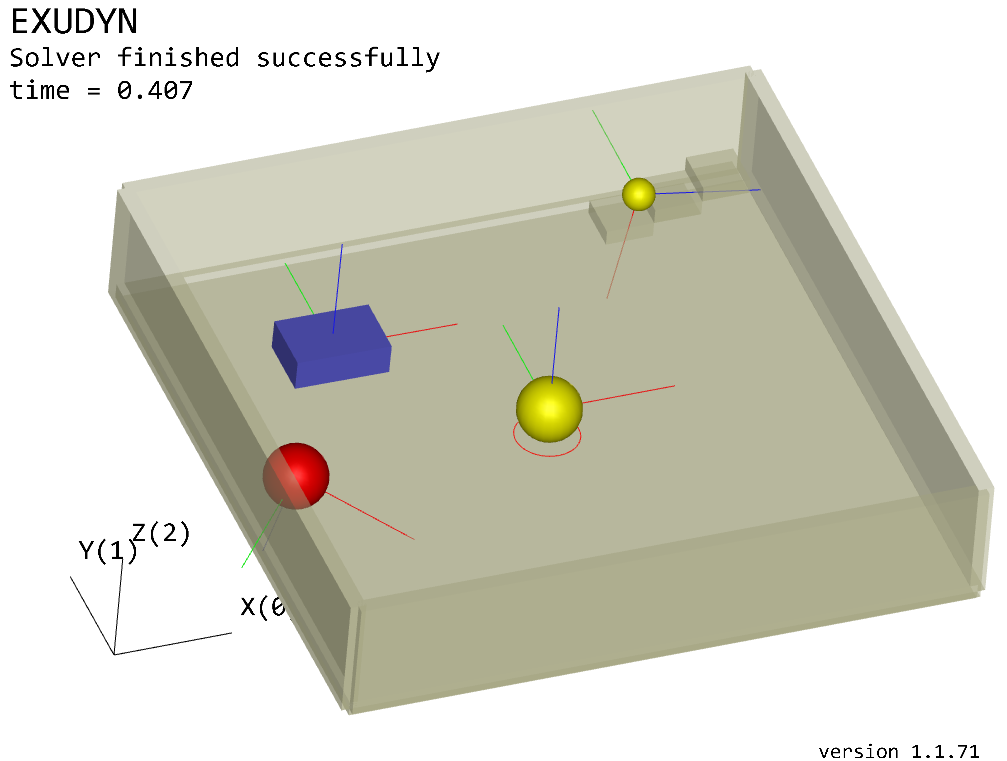
\includegraphics[width=0.35\columnwidth]{figures/contactTests} \hspace{1cm}%
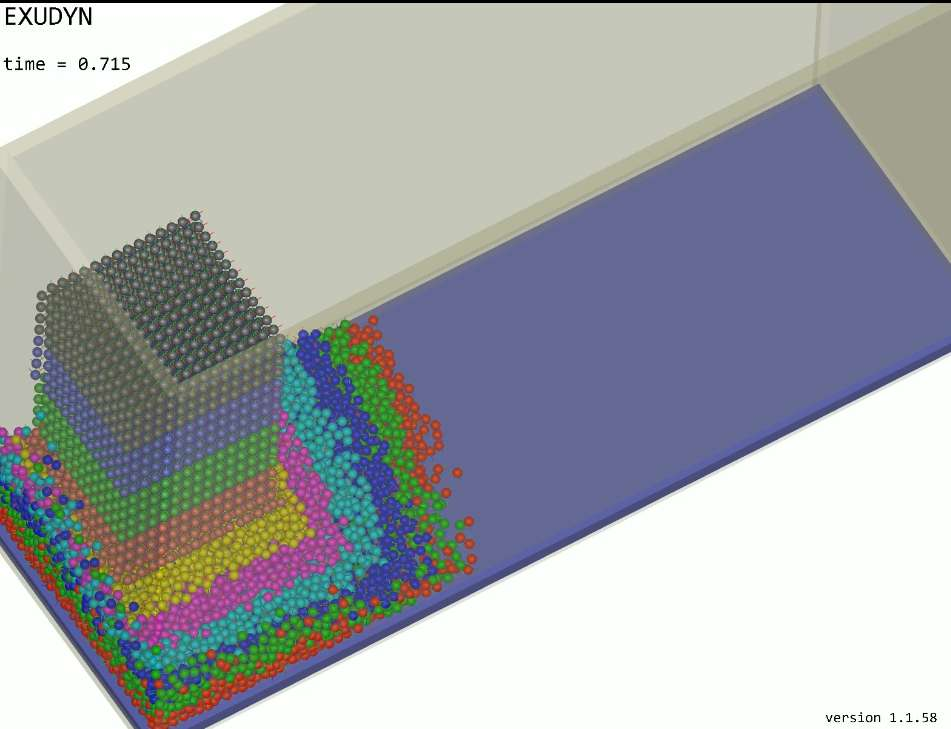
\includegraphics[width=0.35\columnwidth]{figures/contactTests2}%
\end{center}
\caption{Some tests and examples using \texttt{GeneralContact}.}%
\label{fig:contactExamples}%
\end{figure}
}

\noindent \mybold{Note}:
\bi
\item \texttt{GeneralContact} is (in most cases) restricted to dynamic simulation (explicit or implicit $[$\mybold{still under development, consider with care!}$]$) if friction is used; without friction, it also works in the static case
\item in addition to \texttt{GeneralContact} there are special objects, in particular for rolling and simple 1D contacts, that are available as single objects, cf.\ \texttt{ObjectConnectorRollingDiscPenalty}
\item \texttt{GeneralContact} is recommended to be used for large numbers of contacts, while the single objects are integrated more directly into mbs.
\ei

\noindent Currently, \texttt{GeneralContact} includes:
\bi
  \item Sphere-Sphere contact (attached to any marker); may represent circle-circle contact in 2D
  \item Triangles mounted on rigid bodies, in contact with Spheres [only explicit]
  \item ANCFCable2D contacting with spheres (which then represent circles in 2D) [partially implicit, needs revision]
\ei
For details on the contact formulations, see \refSection{secContactTheory}.

%+++++++++++++++++++++++++++++++++++++++++++++++++++++++++++++++++
%+++++++++++++++++++++++++++++++++++++++++++++++++++++++++++++++++
\mysubsubsectionlabel{OpenVR}{sec:overview:advanced:openvr}
%
The general open source libraries from Valve, see
\bi
\item[] https://github.com/ValveSoftware/openvr
\ei
have been linked to \codeName\ . In order to get OpenVR fully integrated, you need to run \texttt{setup.py} \codeName\ with the \texttt{--openvr} flag. For general installation instructions, see \refSection{sec:install:installinstructions}.

Running OpenVR either requires an according head mounted display (HMD) or a virtualization using, e.g., Riftcat 2 to use a mobile phone with an according adapter. Visualization settings are available in \texttt{interactive.openVR}, but need to be considered with care.
An example is provided in \texttt{openVRengine.py}, showing some optimal flags like locking the model rotation, zoom or translation.

Everything is experimental, but contributions are welcome!

%+++++++++++++++++++++++++++++++++++++++++++++++++++++++++++++++++
%+++++++++++++++++++++++++++++++++++++++++++++++++++++++++++++++++
\mysubsubsectionlabel{Interaction with other codes}{sec:overview:advanced:interactwithcodes}
%
Interaction with other codes and computers (E.g., MATLAB or other C++ codes, or other Python versions)
is possible. 
To connect to any other code, it is convenient to use a TCP/IP connection. This is enabled via 
the \texttt{exudyn.utilities} functions
\bi
\item \texttt{CreateTCPIPconnection}
\item \texttt{TCPIPsendReceive}
\item \texttt{CloseTCPIPconnection}
\ei
Basically, data can be transmitted in both directions, e.g., within a preStepUserFunction. In Examples, you can find 
 TCPIPexudynMatlab.py which shows a basic example for such a connectivity.

%+++++++++++++++++++++++++++++++++++++++++++++++++++++++++++++++++
%+++++++++++++++++++++++++++++++++++++++++++++++++++++++++++++++++
\mysubsubsectionlabel{ROS}{sec:overview:advanced:ros}
%
Basic interaction with ROS has been tested. However, make sure to use Python 3, as there is no (and will never be any) Python 2
support for \codeName\ .





%+++++++++++++++++++++++++++++++++++++++++++++++++++++++++++++++++++++++++++++++
%+++++++++++++++++++++++++++++++++++++++++++++++++++++++++++++++++++++++++++++++

\mysubsectionlabel{C++ Code}{sec:overview:cppcode}
This section covers some information on the C++ code. For more information see the Open source code and use doxygen.

Exudyn was developed for the efficient simulation of flexible multi-body systems. Exudyn was designed for rapid implementation and testing of new formulations and algorithms in multibody systems, whereby these algorithms can be easily implemented in efficient C++ code. The code is applied to industry-related research projects and applications.

\mysubsubsection{Focus of the C++ code}
The code focuses on four principles, starting with highest priority: 
\bn
  \item developer-friendly
  \item error minimization
  \item user-friendliness
  \item efficiency
\en
The focus is therefore on:
\bi
    \item A developer-friendly basic structure regarding the C++ class library and the possibility to add new components.
    \item The basic libraries are slim, but extensively tested; only the necessary components are available
    \item Complete unit tests are added to new program parts during development; for more complex processes, tests are available in Python
    \item In order to implement the sometimes difficult formulations and algorithms without errors, error avoidance is always prioritized.
    \item To generate efficient code, classes for parallelization (vectorization and multithreading) are provided. We live the principle that parallelization takes place on multi-core processors with a central main memory, and thus an increase in efficiency through parallelization is only possible with small systems, as long as the program runs largely in the cache of the processor cores. Vectorization is tailored to SIMD commands as they have Intel processors, but could also be extended to GPGPUs in the future.
    \item The user interface (Python) provides a nearly 1:1 image of the system and the processes running in it, which can be controlled with the extensive possibilities of Python.
\ei

\mysubsubsection{C++ Code structure}
%
The following \mybold{entry points} into the C++ code can be found:
\bi
  \item Python -- C++: the creation of the module \texttt{exudyn} is found in:\\
    \texttt{main/src/Pymodules/PybindModule.cpp}\\
  it includes large header files, which are automatically created for binding C++ code with Python.%blank line needed for .rst:
  
  \item The object factory for creation of items (calling \texttt{mbs.AddNode(...)} and similar): \\
    \texttt{main/src/Main/MainObjectFactory.h / .cpp}
  \item Using the VisualStudio \texttt{.sln} file and using the Debug mode allows you to smoothly walk from Python to C++ code (though that this takes some time to start up and it does not work always; and it does not work for graphics if it runs in a separate thread).
\ei

The functionality of the code is mainly based on systems (MainSystem and CSystem), items and solvers representing the multibody system or similar physical systems to be simulated. Parts of the core structure of Exudyn are:
\bi
  \item CSystem / MainSystem: a multibody system which consists of nodes, objects, markers, loads, etc.
  \item SystemContainer: holds a set of systems; connects to visualization (container)
  \item items: node, (computational) object, marker, load, sensor
  \item computational objects: efficient objects for computation = bodies, connectors, connectors, loads, nodes, ...
  \item visualization objects: interface between computational objects and 3D graphics
  \item main (manager) objects: do all tasks (e.g. interface to visualization objects, GUI, Python, ...) which are not needed during computation
  \item static solver, kinematic solver, time integration
  \item Python interface via pybind11; items are accessed with a dictionary interface; system structures and settings read/written by direct access to the structure (e.g. SimulationSettings, VisualizationSettings)
  \item interfaces to linear solvers; future: optimizer, eigenvalue solver, ... (mostly external or in Python)
  \item \mybold{autogenerated}: this folder in \texttt{main/src} contains many item definitions as well as other interface files; they are all automatically generated by some Python code and should not be changed manually as they will be overwritten.
\ei


\mysubsubsection{C++ Code: Modules}
The following internal modules are used, which are represented by directories in \texttt{main/src}:
\bi
  \item Autogenerated: item (nodes, objects, markers and loads) classes split into main (management, Python connection), visualization and computation
  \item Graphics: a general data structure for 2D and 3D graphical objects and a tiny openGL visualization; linkage to GLFW
    \item Linalg: Linear algebra with vectors and matrices; separate classes for small vectors (SlimVector), large vectors (Vector and ResizableVector), vectors without copying data (LinkedDataVector), and vectors with constant size (ConstVector)
  \item Main: mainly contains SystemContainer, System and ObjectFactory
  \item Objects: contains the implementation part of the autogenerated items
  \item Pymodules: manually created libraries for linkage to Python via pybind; remaining linking to Python is located in autogenerated folder
  \item pythonGenerator: contains Python files for automatic generation of C++ interfaces and Python interfaces of items;
  \item Solver: contains all solvers for solving a CSystem
  \item System: contains core item files (e.g., MainNode, CNode, MainObject, CObject, ...)
  \item Tests: files for testing of internal linalg (vector/matrix), data structure libraries (array, etc.) and functions
    \item Utilities: array structures for administrative/managing tasks (indexes of objects ... bodies, forces, connectors, ...); basic classes with templates and definitions
\ei

The following main external libraries are linked to Exudyn:
\bi
  \item LEST: for testing of internal functions (e.g. linalg)
  \item GLFW: 3D graphics with openGL; cross-platform capabilities
  \item Eigen: linear algebra for large matrices, linear solvers, sparse matrices and link to special solvers
  \item pybind11: linking of C++ to Python
\ei

\mysubsubsection{Code style and conventions}
%
This section provides general coding rules and conventions, partly applicable to the C++ and Python parts of the code. Many rules follow common conventions (e.g., google code style, but not always -- see notation):
\bi
    \item write simple code (no complicated structures or uncommon coding)
    \item write readable code (e.g., variables and functions with names that represent the content or functionality; AVOID abbreviations)
    \item put a header in every file, according to Doxygen format
    \item put a comment to every (global) function, member function, data member, template parameter
    \item ALWAYS USE curly brackets for single statements in 'if', 'for', etc.; example: if (i<n) \{i += 1;\}
    \item use Doxygen-style comments (use '//!' Qt style and '@ date' with '@' instead of '\' for commands)
    \item use Doxygen (with preceeding '@') 'test' for tests, 'todo' for todos and 'bug' for bugs
    \item USE 4-spaces-tab
    \item use C++11 standards when appropriate, but not exhaustively
    \item ONE class ONE file rule (except for some collectors of single implementation functions)
    \item add complete unit test to every function (every file has link to LEST library)
    \item avoid large classes (>30 member functions; > 15 data members)
    \item split up god classes (>60 member functions)
    \item mark changed code with your name and date
    \item REPLACE tabs by spaces: Extras->Options->C/C++->Tabstopps: tab stopp size = 4 (=standard) +  KEEP SPACES=YES
\ei

\mysubsubsection{Notation conventions}
%
The following notation conventions are applied (\mybold{no exceptions!}):
\bi
    \item use lowerCamelCase for names of variables (including class member variables), consts, c-define variables, ...; EXCEPTION: for algorithms following formulas, e.g., $f = M*q_{tt} + K*q$, GBar, ...
    \item use UpperCamelCase for functions, classes, structs, ...
    \item Special cases for CamelCase (with some exceptions that happened in the past ...): 
    \bi
    \item continue upper case after upper case abbreviations in case of \mybold{functions or classes}: 'ODESystem', 'Point2DClass', 'ANCFCable2D', 'ANCFALE', 'ComputeODE1Equations', ... (this is not always nice to read, but has become a standard and will be further used!) 
    \item for variables and class member variables continue \mybold{lower case}: 'nODE1variables', 'dim2Dspecial', 'ANCFsize'
    \item abbreviations at beginning of expressions: for functions or classes use \texttt{ODEComputeCoords()}, for variables avoid 'ODE' at beginning: use 'nODE' or write 'odeCoordinates'
    \ei
    \item '[...]Init' ... in arguments, for initialization of variables; e.g. 'valueInit' for initialization of member variable 'value'
    \item use American English throughout: Visualization, etc.
    \item AVOID consecutive capitalized words, e.g., avoid 'ODEAE'
    \item do not use '\_' within variable or function names; exception: derivatives
    \item use name which exactly describes the function/variable: 'numberOfItems' instead of 'size' or 'l'
    \item examples for variable names: secondOrderSize, massMatrix, mThetaTheta
    \item examples for function/class names: \texttt{SecondOrderSize}, \texttt{EvaluateMassMatrix}, \texttt{Position(const Vector3D\& localPosition)}
    \item use the Get/Set...() convention if data is retrieved from a class (Get) or something is set in a class (Set); Use \texttt{const T\& Get()/T\& Get} if direct access to variables is needed; Use Get/Set for pybind11
    \item example Get/Set: \texttt{Real* GetDataPointer()}, \texttt{Vector::SetAll(Real)}, \texttt{GetTransposed()}, \texttt{SetRotationalParameters(...)}, \texttt{SetColor(...)}, ...
    \item use 'Real' instead of double or float: for compatibility, also for AVX with SP/DP
    \item use 'Index' for array/vector size and index instead of size\_t or int
    \item item: object, node, marker, load: anything handled within the computational/visualization systems
    \item Do not use numbers (3 for 3D or any other number which represents, e.g., the number of rotation parameters). Use const Index or constexpr to define constants.
\ei

\mysubsubsection{No-abbreviations-rule}
%
The code uses a \mybold{minimum set of abbreviations}; however, the following abbreviation rules are used throughout:
In general: DO NOT ABBREVIATE function, class or variable names: GetDataPointer() instead of GetPtr(); exception: cnt, i, j, k, x or v in cases where it is really clear (short, 5-line member functions).

\mybold{Exceptions} to the NO-ABBREVIATIONS-RULE, see also \hyperref[sec:listOfAbbreviations]{\underline{List of Abbreviations}}: %no section number!!!: \refSection{sec:listOfAbbreviations}
\bi
    \item \ac{ODE}
    \item \ac{ODE2}: marks parts related to second order differential equations (SOS2, EvalF2 in HOTINT)
    \item \ac{ODE1}: marks parts related to first order differential equations (ES, EvalF in HOTINT)
    \item \ac{AE}; note: using the term 'AEcoordinates' for 'algebraicEquationsCoordinates'
    \item 'C[...]' ... Computational, e.g. for ComputationalNode ==> use 'CNode'
    \item \ac{mbs}
    \item \ac{min}, \ac{max}
    \item \ac{abs}, \ac{rel}
    \item \ac{trig} 
    \item \ac{quad}
    \item \ac{RHS}
    \item \ac{LHS}
    \item \ac{EP}
    \item \ac{Rxyz}%: consecutive rotations around x, y and z-axis (Tait-Bryan rotations);
    \item \ac{coeffs}
    \item \ac{pos}
    \item \ac{T66}; based on $6\times 6$ matrix transformations
    \item write time derivatives with underscore: \_t, \_tt; example: Position\_t, Position\_tt, ...
    \item write space-wise derivatives ith underscore: \_x, \_xx, \_y, ...
    \item if a scalar, write coordinate derivative with underscore: \_q, \_v (derivative w.r.t. velocity coordinates)
    \item for components, elements or entries of vectors, arrays, matrices: use 'item' throughout
    \item '[...]Init' ... in arguments, for initialization of variables; e.g. 'valueInit' for initialization of member variable 'value'
\ei

%+++++++++++++++++++++++++++++++++++++++++++++++++++++++++++++++++++++++++++++++
%+++++++++++++++++++++++++++++++++++++++++++++++++++++++++++++++++++++++++++++++

\mysubsubsection{Implementation of new computational items in C++}
%
This section should sketch which changes will be needed to integrate new C++ items.
In general, it is recommended to first start with a Python implementation with user functions based on
\texttt{NodeGeneric...}, \texttt{ObjectGeneric...}, \texttt{ObjectConnectorCoordinateVector} for constraints and
any suitable connector for new nodes or objects. New sensors can be based on the \texttt{SensorUserFunction}.

If such an implementation is successful, but too slow, a C++ implementation can be considered.
In the following, two use cases are shown, which show the simplicity of the procedure:
\bi
  \item \mybold{Case 1}: user object (body):\\
  It is recommended to first search for a body with a similar behavior.
  Copy the definition of such an object inside the file \texttt{objectDefinition.py} and edit the according lines. 
  There is not much description of 
  this file yet (except from the first lines of the file), as it will be transformed into another format in the future.
  Basically, you need to edit the interface, which contains parameters (which are linked to Python) and functions, 
  which go to the header file.
  When you finished editing, run \texttt{pythonAutoGenerateObjects.py}. This generates the header file in \texttt{src/autogenerated}
  but also adds description to some docs files and adds the \texttt{pybind11} interface. 
  Now copy the implementation (\texttt{.cpp}) file of the same connector from which you copied from and rename and edit all functions.
  %
  For the body
  \bi
    \item \texttt{ComputeMassMatrix}: computes the mass matrix either in sparse or dense mode; this function is performance-critical if the mass matrix is non-constant
    \item \texttt{ComputeODE2LHS}: computes the \ac{LHS} generalized forces of the body; this function is performance-critical
    \item \texttt{GetAccessFunctionTypes}: specifies, which access functions are available in \texttt{GetAccessFunctionBody(...)}
    \item \texttt{GetAccessFunctionBody}: needs to compute functions for 'access' to the body, in the sense that e.g.\ forces or torques can be applied. 
    \item \texttt{GetAvailableJacobians}: shall return the flags which jacobians of \texttt{ComputeODE2LHS} need to be computed and which are available as functions; binary flags added up
    \item \texttt{GetOutputVariableBody}: function needs to implement the output variables, such as position, acceleration, forces, etc.\ as defined in \texttt{GetOutputVariableTypes()}
    \item \texttt{HasConstantMassMatrix}: specifies, if mass matrix is constant
    \item \texttt{GetNumberOfNodes}: number of nodes of object
    \item \texttt{GetODE2Size}: total number of \ac{ODE2} coordinates
    \item \texttt{GetType}: some flags for objects, such as \texttt{Body}, \texttt{SingleNoded}, \texttt{SuperElement}, ...; these flags are needed for connectivity and special treatment in the system
    \item \texttt{GetPosition, GetVelocity, ...}: provide this functions as far as possible; rigid bodies need to provide positions and rotation matrix, as well as velocity and angular velocity for markers; if functions do not exist, some marker or sensor functions may fail
    \item ...   possibly some helper functions, which you should implement for the functionality of your object.
  \ei
  \item \mybold{Case 2}: user connector:\\
  It is recommended to search for a connector with similar behavior; first check, if you would like to implement 
  an algebraic constraint or a spring-damper-like connector.
  Again, copy a similar connector in \texttt{objectDefinition.py} and edit the according lines. 
  When you finished editing, run \texttt{pythonAutoGenerateObjects.py} and make a copy of the copied implementation (\texttt{.cpp}) file.
  The implementation file usually consists of
  \bi
    \item \texttt{ComputeODE2LHS}: this function shall compute the \ac{LHS} generalized forces on the two marker objects
    \item \texttt{ComputeJacobianODE2\_ODE2}: computes the \texttt{GetAvailableJacobians()} is not providing any '...\_function' flag, which indicates that these jacobians are available as function
    \item \texttt{GetOutputVariableConnector}: this function needs to compute all output variables as given in \texttt{GetOutputVariableTypes()}
    \item ...   possibly some helper functions, which you should implement for the functionality of your object.
  \ei
\ei



%+++++++++++++++++++++++++++++++++++++++++++++++++++++++++++++++++++++++++++++++
%+++++++++++++++++++++++++++++++++++++++++++++++++++++++++++++++++++++++++++++++

%\ignoreRST{
%\mysubsection{Changes}
%\label{sec:changes}
%For continuous tracking of changes, see \refSection{sec:issueTracker}.
%}


%+++++++++++++++++++++++++++++++++++++++++++++++++++++++++++++++++++++++++++++++
%+++++++++++++++++++++++++++++++++++++++++++++++++++++++++++++++++++++++++++++++
\mysection{Tutorial}
%
This section will show:
\bi
  \item A basic tutorial for a 1D mass and spring-damper with initial displacements, shortest possible model with practically no special settings
  \item A more advanced rigid-body model, including 3D rigid bodies and revolute joints
  \item Links to examples section
\ei
%
A large number of examples, some of them quite advanced, can be found in:
\bi
  \item[] \texttt{main/pythonDev/Examples}
  \item[] \texttt{main/pythonDev/TestModels}
\ei

%+++++++++++++++++++++++++++++++++++++++++++++++++++++++++++++++++++++++++++++++
%+++++++++++++++++++++++++++++++++++++++++++++++++++++++++++++++++++++++++++++++
\mysubsection{Mass-Spring-Damper tutorial}
The Python source code of the first tutorial can be found in the file:
\bi
  \item[] \texttt{main/pythonDev/Examples/springDamperTutorial.py}
\ei
A similar version based on a simplified approach (using a 3D mass point) is available as, which uses simplified approaches:
\bi
  \item[] \texttt{main/pythonDev/Examples/springDamperTutorialNew.py}
\ei
The following tutorial will set up a mass point and a spring damper, dynamically compute the solution and evaluate the reference solution.
\vspace{6pt}\\
We import the exudyn library and the interface for all nodes, objects, markers, loads and sensors:
\pythonstyle\begin{lstlisting}
  import exudyn as exu
  from exudyn.utilities import Point, NodePointGround, MassPoint, MarkerNodeCoordinate,\
                               CoordinateSpringDamper, LoadCoordinate, SensorObject
  import exudyn.graphics as graphics #only import if it does not conflict
  import numpy as np #for postprocessing
\end{lstlisting}
%
Instead of the named import of \texttt{exudyn.utilities} functions and classes, you can use a star import,
which includes \texttt{itemInterface}, \texttt{rigidBodyUtilities} and some helper functions:
\pythonstyle\begin{lstlisting}
  from exudyn.utilities import *
\end{lstlisting}
%
Next, we need a \texttt{SystemContainer}, which contains all computable systems and add a new MainSystem \texttt{mbs}.
Per default, you always should name your system 'mbs' (multibody system), in order to copy/paste code parts from other examples, tutorials and other projects:
\pythonstyle\begin{lstlisting}
  SC = exu.SystemContainer()
  mbs = SC.AddSystem()
\end{lstlisting}
%
In order to check, which version you are using, you can printout the current \codeName\ version. 
The version shown is in line with the issue tracker and marks the number of open/closed issues added to \codeName\ .
Adding \texttt{True} as argument will also print platform-specific information, which is helpful 
in case of reporting some compatibility issues:
\pythonstyle\begin{lstlisting}
  print('EXUDYN version='+exu.config.Version(True))
\end{lstlisting}
%
Using the powerful Python language, we can define some variables for our problem, which will also be used for the analytical solution:
\pythonstyle\begin{lstlisting}
  L=0.5               #reference position of mass
  mass = 1.6          #mass in kg
  spring = 4000       #stiffness of spring-damper in N/m
  damper = 8          #damping constant in N/(m/s)
  f =80               #force on mass
\end{lstlisting}
%
For the simple spring-mass-damper system, we need initial displacements and velocities:
\pythonstyle\begin{lstlisting}
  u0=-0.08            #initial displacement
  v0=1                #initial velocity
  x0=f/spring         #static displacement
  print('resonance frequency = '+str(np.sqrt(spring/mass)))
  print('static displacement = '+str(x0))
\end{lstlisting}
%
We first need to add nodes, which provide the coordinates (and the degrees of freedom) to the system.
The following line adds a 3D node for 3D mass point\footnote{Note: Point is an abbreviation for NodePoint, defined in \texttt{itemInterface.py}.}:
\pythonstyle\begin{lstlisting}
  n1=mbs.AddNode(Point(referenceCoordinates = [L,0,0], 
                       initialCoordinates = [u0,0,0], 
                       initialVelocities = [v0,0,0]))
\end{lstlisting}
Here, \texttt{Point} (=\texttt{NodePoint}) is a Python class, which takes a number of arguments defined in the reference manual. The arguments here are \texttt{referenceCoordinates}, which are the coordinates for which the system is defined. The initial configuration is given by \texttt{referenceCoordinates + initialCoordinates}, while the initial state additionally gets \texttt{initialVelocities}.
The command \texttt{mbs.AddNode(...)} returns a \texttt{NodeIndex n1}, which basically contains an integer, which can only be used as node number. This node number will be used lateron to use the node in the object or in the marker.

%
While \texttt{Point} adds 3 unknown coordinates to the system, which need to be solved, we also can add ground nodes, which can be used similar to nodes, but they do not have unknown coordinates -- and therefore also have no initial displacements or velocities. The advantage of ground nodes (and ground bodies) is that no constraints are needed to fix these nodes.
%
Such a ground node is added via:
\pythonstyle\begin{lstlisting}
  nGround=mbs.AddNode(NodePointGround(referenceCoordinates = [0,0,0]))
\end{lstlisting}
%
In the next step, we add an object\footnote{For the moment, we just need to know that objects either depend on one or more nodes, which are usually bodies and finite elements, or they can be connectors, which connect (the coordinates of) objects via markers, see \refSection{sec:overview:modulestructure}.}, which provides equations for coordinates. The \texttt{MassPoint} needs at least a mass (kg) and a node number to which the mass point is attached. Additionally, graphical objects could be attached:
\pythonstyle\begin{lstlisting}
  massPoint = mbs.AddObject(MassPoint(physicsMass = mass, nodeNumber = n1))
\end{lstlisting}
Note that instead of adding a \texttt{NodePoint} and a \texttt{MassPoint} with \texttt{mbs.AddNode(...)}
and \texttt{mbs.AddObject(...)}, there is also a convenient function \texttt{mbs.CreateMassPoint(...)}, which can do everything at once including the option to add gravity.

In order to apply constraints and loads, we need markers. These markers are used as local positions (and frames), where we can attach a constraint lateron. In this example, we work on the coordinate level, both for forces as well as for constraints.
Markers are attached to the according ground and regular node number, additionally using a coordinate number (0 ... first coordinate):
\pythonstyle\begin{lstlisting}
  groundMarker=mbs.AddMarker(MarkerNodeCoordinate(nodeNumber= nGround, 
                                                  coordinate = 0))
  #marker for springDamper for first (x-)coordinate:
  nodeMarker = mbs.AddMarker(MarkerNodeCoordinate(nodeNumber= n1, 
                                                  coordinate = 0))
\end{lstlisting}
This means that constraints are be applied to the first coordinate of node \texttt{n1} via marker with number \texttt{nodeMarker}, which is in fact of type \texttt{MarkerNodeCoordinate}.

Now we add a spring-damper to the markers with numbers \texttt{groundMarker} and the \texttt{nodeMarker}, providing stiffness and damping parameters:
\pythonstyle\begin{lstlisting}
  nC = mbs.AddObject(CoordinateSpringDamper(markerNumbers = [groundMarker, nodeMarker], 
                                       stiffness = spring, 
                                       damping = damper)) 
\end{lstlisting}
%
A load is added to marker \texttt{nodeMarker}, with a scalar load with value \texttt{f}:
\pythonstyle\begin{lstlisting}
  nLoad = mbs.AddLoad(LoadCoordinate(markerNumber = nodeMarker, 
                                     load = f))
\end{lstlisting}
Again, instead of adding a \texttt{MarkerNodeCoordinate} and a \texttt{LoadCoordinate} with \texttt{mbs.AddLoad(...)},
we could just use \texttt{mbs.CreateForce(...)} to add a 3D force vector.
For specific joints, there are also \texttt{mbs.Create...(...)} functions.

Finally, a sensor is added to the coordinate constraint object with number \texttt{nC}, requesting the \texttt{outputVariableType} \texttt{Force}:
\pythonstyle\begin{lstlisting}
  mbs.AddSensor(SensorObject(objectNumber=nC, fileName='groundForce.txt', 
                             outputVariableType=exu.OutputVariableType.Force))
\end{lstlisting}
Note that sensors can be attached, e.g., to nodes, bodies, objects (constraints) or loads.
%
As our system is fully set, we can print the overall information and assemble the system to make it ready for simulation:
\pythonstyle\begin{lstlisting}
  print(mbs)     #show system properties
  mbs.Assemble() #prepare for simulation
\end{lstlisting}
%
We will use time integration and therefore define a number of steps (fixed step size; must be provided) and the total time span for the simulation:
\pythonstyle\begin{lstlisting}
  tEnd = 1     #end time of simulation
  h = 0.001    #step size; leads to 1000 steps
\end{lstlisting}
%
All settings for simulation, see according reference section, can be provided in a structure given from \texttt{exu.SimulationSettings()}. Note that this structure will contain all default values, and only non-default values need to be provided:
\pythonstyle\begin{lstlisting}
  simulationSettings = exu.SimulationSettings()
  simulationSettings.solutionSettings.solutionWritePeriod = 5e-3 #output interval general
  simulationSettings.solutionSettings.sensorsWritePeriod = 5e-3  #output interval of sensors
  simulationSettings.timeIntegration.numberOfSteps = tEnd/h
  simulationSettings.timeIntegration.endTime = tEnd
  simulationSettings.displayComputationTime = True               #show how fast
\end{lstlisting}
%
In order to see some solver output, we must set \texttt{verboseMode} to 1 (higher values gives detailed output per step).
Furthermore, we can show information on computation time (which may cost some overhead in computation!):
\pythonstyle\begin{lstlisting}
  simulationSettings.timeIntegration.verboseMode = 1             #show some solver output
  simulationSettings.displayComputationTime = True               #show how fast
\end{lstlisting}
We are using a generalized alpha solver, where numerical damping is needed for index 3 constraints. As we have only spring-dampers, we can set the spectral radius to 1, meaning no numerical damping:
\pythonstyle\begin{lstlisting}
  simulationSettings.timeIntegration.generalizedAlpha.spectralRadius = 1
\end{lstlisting}
%
In order to visualize the results online, a renderer can be started. As our computation will be very fast, it is a good idea to wait for the user to press SPACE, before starting the simulation (uncomment second line):
\pythonstyle\begin{lstlisting}
  SC.renderer.Start()              #start graphics visualization
  #SC.renderer.DoIdleTasks()       #wait for SPACE bar or 'Q' to continue (in render window!)
\end{lstlisting}
As the simulation is still very fast, we will not see the motion of our node. Using a very small step size of, e.g., \texttt{h=1e-7} in the lines above allows us to visualize the resulting oscillations in realtime.

%
Finally, we start the solver, by telling which system to be solved, solver type and the simulation settings:
\pythonstyle\begin{lstlisting}
  exu.SolveDynamic(mbs, simulationSettings)
\end{lstlisting}
%

After simulation, our renderer needs to be stopped (otherwise it will stop unsafely as soon as the Python kernel is stopped or restarted). 
Sometimes you would like to wait until closing the render window, using \texttt{WaitForRenderEngineStopFlag()}:
\pythonstyle\begin{lstlisting}
  #SC.renderer.DoIdleTasks()       #wait for pressing 'Q' to quit
  SC.renderer.Stop()               #safely close rendering window!
\end{lstlisting}
%
If you run this code, e.g. in Spyder or Visual Studio Code, it may take a 1-2 seconds to complete. However, the time spent is only related to some overhead in the Python environment and for the visualization. The simulation itself will only take around 3-10 milliseconds, in which a large overhead is due to file writing.

There are several ways to evaluate results, see the reference pages. In the following we take the final value of node \texttt{n1} and read its 3D position vector:
\pythonstyle\begin{lstlisting}
  #evaluate final (=current) output values
  u = mbs.GetNodeOutput(n1, exu.OutputVariableType.Position)
  print('displacement=',u)
\end{lstlisting}
%
The following code generates a reference (exact) solution for our example:
\pythonstyle\begin{lstlisting}
  import matplotlib.pyplot as plt
  import matplotlib.ticker as ticker

  omega0 = np.sqrt(spring/mass)          #eigen frequency of undamped system
  dRel = damper/(2*np.sqrt(spring*mass)) #dimensionless damping
  omega = omega0*np.sqrt(1-dRel**2)      #eigen freq of damped system
  C1 = u0-x0 #static solution needs to be considered!
  C2 = (v0+omega0*dRel*C1) / omega       #C1, C2 are coeffs for solution
  steps = int(tEnd/h)                    #use same steps for reference solution

  refSol = np.zeros((steps+1,2))
  for i in range(0,steps+1):
    t = tEnd*i/steps
    refSol[i,0] = t
    refSol[i,1] = np.exp(-omega0*dRel*t)*(C1*np.cos(omega*t)+C2*np.sin(omega*t))+x0

  plt.plot(refSol[:,0], refSol[:,1], 'r-', label='displacement (m); exact solution')
\end{lstlisting}
%
Now we can load our results from the default solution file \texttt{coordinatesSolution.txt}, which is in the same
directory as your Python tutorial file. 
\mybold{Note} that the visualization of results can be simplified considerably using the \texttt{PlotSensor(...)} utility function as shown in the \mybold{Rigid body and joints tutorial}!

For reading the file containing commented lines (this does not work in binary mode!), we use a numpy feature and finally plot the displacement of coordinate 0 or our mass point\footnote{\texttt{data[:,0]} contains the simulation time, \texttt{data[:,1]} contains displacement of (global) coordinate 0, \texttt{data[:,2]} contains displacement of (global) coordinate 1, ...)}:
\pythonstyle\begin{lstlisting}
  data = np.loadtxt('coordinatesSolution.txt', comments='#', delimiter=',')
  plt.plot(data[:,0], data[:,1], 'b-', label='displacement (m); numerical solution') 
\end{lstlisting}
Note that the coordinates do not include the reference position (which is 0.5 in this case). For information on displacement and reference coordinates, see \refSection{sec:overview:items:coordinates}.

The sensor result can be loaded in the same way. The sensor output format contains time in the first column and sensor values in the remaining columns. The number of columns depends on the 
sensor and the output quantity (scalar, vector, ...):
\pythonstyle\begin{lstlisting}
  data = np.loadtxt('groundForce.txt', comments='#', delimiter=',')
  plt.plot(data[:,0], data[:,1]*1e-3, 'g-', label='force (kN)')
\end{lstlisting}
%
In order to get a nice plot within Spyder, the following options can be used\footnote{note, in some environments you need finally the command \texttt{plt.show()}}:
\pythonstyle\begin{lstlisting}
  ax=plt.gca() # get current axes
  ax.grid(True, 'major', 'both')
  ax.xaxis.set_major_locator(ticker.MaxNLocator(10))
  ax.yaxis.set_major_locator(ticker.MaxNLocator(10))
  plt.legend() #show labels as legend
  plt.tight_layout()
  plt.show() 
\end{lstlisting}
%
The matplotlib output should look as shown in \fig{fig_tutorial_springDamper}.
%
\LatexRSTfigure{figures/plotSpringDamper}{fig_tutorial_springDamper}{12cm}{400}{Output of spring-damper tutorial.}
%
%
%\ignoreRST{\begin{center}
  %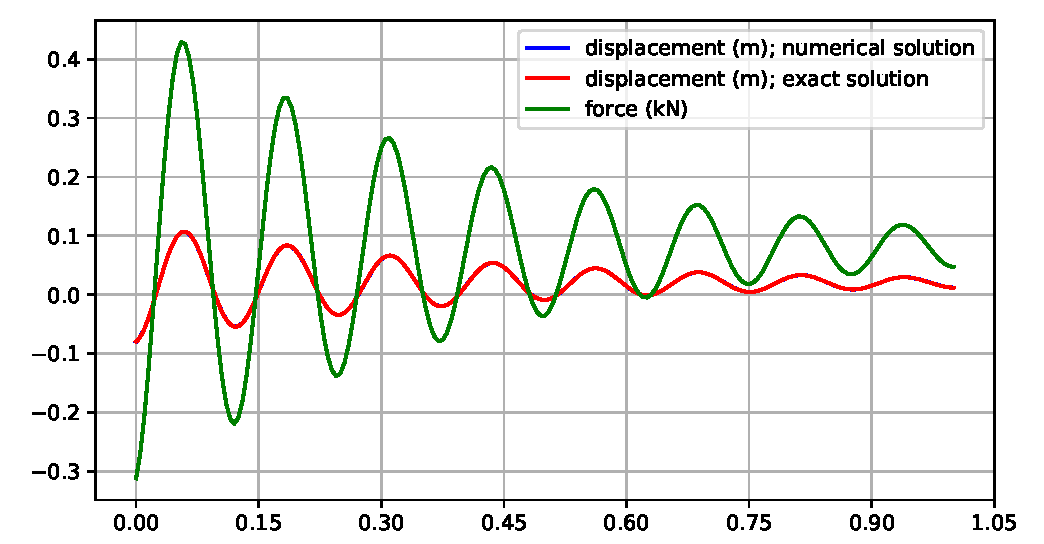
\includegraphics[height=6cm]{../demo/screenshots/plotSpringDamper}
%\end{center}}
%\onlyRST{
%
%.. image:: docs/theDoc/figures/plotSpringDamper.png
   %:width: 400
%
%}



%++++++++++++++++++++++++++++++++++++++++++++++++++++++++++++++++++++++++++++++++++++++++++++++++++++++++++++++
%++++++++++++++++++++++++++++++++++++++++++++++++++++++++++++++++++++++++++++++++++++++++++++++++++++++++++++++
%++++++++++++++++++++++++++++++++++++++++++++++++++++++++++++++++++++++++++++++++++++++++++++++++++++++++++++++
\newpage
\mysubsectionlabel{Rigid body and joints tutorial}{sec:tutorial:rigidBodyJoints}
The Python source code of the first tutorial, based on the simple description of revolute joints, can be found in the file:
\bi
  \item[] \texttt{main/pythonDev/Examples/rigidBodyTutorial3.py}
\ei
For alternative approaches, see
\bi
  \item[] \texttt{main/pythonDev/Examples/rigidBodyTutorial3withMarkers.py}
  \item[] \texttt{main/pythonDev/Examples/rigidBodyTutorial2.py}
\ei
\mybold{NOTE} that the youtube video uses a slightly older way of creating graphics using \texttt{GraphicsData...} functions, which
can be easily replaced by the newer \texttt{graphics. ...} commands shown here. Their interface is identical.

This tutorial will set up a multibody system containing a ground, two rigid bodies and two revolute joints driven by gravity, compare a 3D view of the example in \fig{fig_RigidBodyTutorialView}.
%
\LatexRSTfigure{figures/TutorialRigidBody1desc}{fig_RigidBodyTutorialView}{14cm}{400}{Render view of rigid body tutorial, showing objects, nodes (N0, N1), and loads.}
%
%\ignoreRST{\fig{fig_RigidBodyTutorialView}.} \onlyRST{the figure above.}
%\ignoreRST{\begin{figure}[tbph]
  %\begin{center}
    %\includegraphics[width=0.9\textwidth]{figures/TutorialRigidBody1desc}
  %\end{center}
  %\caption{Render view of rigid body tutorial, showing objects, nodes (N0, N1), and loads.}
  %\label{fig_RigidBodyTutorialView}
%\end{figure}}
%\onlyRST{
%
%.. image:: docs/theDoc/figures/TutorialRigidBody1desc.png
%   :width: 400
%
%}
\horizontalRuler\\
\noindent We first import the exudyn library and the interface for all nodes, objects, markers, loads and sensors:
\pythonstyle\begin{lstlisting}
  import exudyn as exu
  #import specific items, inertia class for general cuboid (hexahedral) block, etc.
  from exudyn.utilities import InertiaCuboid, ObjectRigidBody, MarkerBodyRigid, \
                               GenericJoint, VObjectJointGeneric, SensorBody
  import exudyn.graphics as graphics #only import as graphics if it does not conflict
  import numpy as np #for postprocessing
\end{lstlisting}
The submodule \texttt{exudyn.utilities} contains helper functions for graphics representation, 3D rigid bodies and joints.
For simplicity, many examples just use a star import instead, which is recommended for rapid model development:
\pythonstyle\begin{lstlisting}
  from exudyn.utilities import *
\end{lstlisting}


\noindent As in the first tutorial, we need a \texttt{SystemContainer} and add a new MainSystem \texttt{mbs}:
\pythonstyle\begin{lstlisting}
  SC = exu.SystemContainer()
  mbs = SC.AddSystem()
\end{lstlisting}

\noindent We define some geometrical parameters for lateron use.
\pythonstyle\begin{lstlisting}
  #physical parameters
  g =     [0,-9.81,0] #gravity
  L = 1               #length
  w = 0.1             #width
  bodyDim=[L,w,w]     #body dimensions
  p0 =    [0,0,0]     #origin of pendulum
  pMid0 = np.array([L*0.5,0,0]) #center of mass, body0
\end{lstlisting}

\noindent We add an empty ground body, using default values. It's origin is at [0,0,0] and here we use no visualization.
\pythonstyle\begin{lstlisting}
  #ground body, located at specific position (there could be several ground objects)
  oGround = mbs.CreateGround(referencePosition=[0,0,0])
\end{lstlisting}
On the background, the \texttt{CreateGround} function creates an object, which is equivalent to:
\pythonstyle\begin{lstlisting}
  oGround = mbs.AddObject(ObjectGround(referencePosition=[0,0,0]))
\end{lstlisting}

\horizontalRuler\\
\noindent For physical parameters of the rigid body, we can use the class \texttt{RigidBodyInertia}, which allows to define mass, center of mass (COM) and inertia parameters, as well as shifting COM or adding inertias.
The \texttt{RigidBodyInertia} can be used directly to create rigid bodies. Special derived classes can be use to define rigid body inertias for cylinders, cubes, etc., so we use a cube here:
\pythonstyle\begin{lstlisting}
  #first link:
  #inertia for cubic body with dimensions in sideLengths
  iCube0 = InertiaCuboid(density=5000, sideLengths=bodyDim)
  iCube0 = iCube0.Translated([-0.25*L,0,0]) #transform COM, COM not at reference point!
\end{lstlisting}
Note that the COM is translated in axial direction, while it would be at the body's local position [0,0,0] by default!

\noindent For visualization, we add some graphics for the body defined as a 3D cube with center point and dimensions; additionally we draw a basis (three RGB-vectors) at the COM:
\pythonstyle\begin{lstlisting}
  #graphics for body
  graphicsBody0 = graphics.Brick(centerPoint=[0,0,0],size=[L,w,w],
                                 color=graphics.color.red)
  graphicsCOM0 = graphics.Basis(origin=iCube0.com, length=2*w)
\end{lstlisting}

\noindent Now we have defined all data for the link (rigid body). We could use \texttt{mbs.AddNode(NodeRigidBodyEP(...))} and \texttt{mbs.AddObject(ObjectRigidBody(...))} to create a node and a body, but the \texttt{MainSystem} since V1.6.110 offers a much more comfortable function:
\pythonstyle\begin{lstlisting}
  #create node, add body and gravity load:
  b0=mbs.CreateRigidBody(inertia = iCube0, #includes COM
                         referencePosition = pMid0,
                         gravity = g,
                         graphicsDataList = [graphicsCOM0, graphicsBody0])
\end{lstlisting}
which also adds a gravity load and could also set initial velocities, if wanted. Note that much more options are available for this function, e.g.,
we could define a \texttt{nodeType} for the underlying formulation of the rigid body node, see \refSection{sec:NodeType}.
We can use 
\bi
\item \texttt{RotationEulerParameters}: for fast computation, but leads to an additional algebraic equation and thus needs an implicit solver
\item \texttt{RotationRxyz}: contains a singularity if the second angle reaches +/- 90 degrees, but no algebraic equations
\item \texttt{RotationRotationVector}: for usage with Lie group integrators, especially with explicit integration, singularities are bypassed; leads to fewest unknowns and usually less Newton iterations
\ei

\noindent We now add a revolute joint around the (global) z-axis. 
We have several possibilities, which are shown in the following.
For the \mybold{first two possibilities only}, following \texttt{rigidBodyTutorial3withMarkers.py}, we need the following markers
\pythonstyle\begin{lstlisting}
  #markers for ground and rigid body (not needed for option 3):
  markerGround = mbs.AddMarker(MarkerBodyRigid(bodyNumber=oGround, localPosition=[0,0,0]))
  markerBody0J0 = mbs.AddMarker(MarkerBodyRigid(bodyNumber=b0, localPosition=[-0.5*L,0,0]))
\end{lstlisting}

\noindent The very general \mybold{option 1} is to use the \texttt{GenericJoint}, that can be used to define any kind of joint with translations and rotations fixed or free,
\pythonstyle\begin{lstlisting}
  #revolute joint option 1:
  mbs.AddObject(GenericJoint(markerNumbers=[markerGround, markerBody0J0], 
                             constrainedAxes=[1,1,1,1,1,0],
                             visualization=VObjectJointGeneric(axesRadius=0.2*w, 
                                                               axesLength=1.4*w)))
\end{lstlisting}
In addition, transformation matrices (\texttt{rotationMarker0/1}) can be added, see the joint description.

\noindent \mybold{Option 2} is using the revolute joint, which allows a free rotation around the local z-axis of marker 0 (\texttt{markerGround} in our example)
\pythonstyle\begin{lstlisting}
  #revolute joint option 2:
  mbs.AddObject(ObjectJointRevoluteZ(markerNumbers = [markerGround, markerBody0J0], 
                                     rotationMarker0=np.eye(3),
                                     rotationMarker1=np.eye(3),
                                     visualization=VObjectJointRevoluteZ(axisRadius=0.2*w, 
                                                                         axisLength=1.4*w)
                                     )) 
\end{lstlisting}
Additional transformation matrices (\texttt{rotationMarker0/1}) can be added in order to chose any rotation axis.

\noindent Note that an error in the definition of markers for the joints can be also detected in the render window (if you completed the example), e.g., if you change the following marker in the lines above,
\pythonstyle\begin{lstlisting}
  #example if wrong marker position is chosen:
  markerBody0J0 = mbs.AddMarker(MarkerBodyRigid(bodyNumber=b0, localPosition=[-0.4*L,0,0]))
\end{lstlisting}
$\ra$ you will see a misalignment of the two parts of the joint by \texttt{0.1*L}.
The latter approach is very general and will also work for any kind of flexible bodies.

\noindent Due to the fact that the definition of markers for general joints is tedious, \mybold{option 3} is based on a MainSystem function, which allows to attach revolute joints immediately to \mybold{rigid bodies} and defining the rotation axis only once for the joint:
\pythonstyle\begin{lstlisting}
  #revolute joint option 3 (simplest):
  mbs.CreateRevoluteJoint(bodyNumbers=[oGround, b0], position=[0,0,0], 
                          axis=[0,0,1], axisRadius=0.2*w, axisLength=1.4*w)
\end{lstlisting}
Note that \texttt{axis} and \texttt{position} are defined in global coordinates, and local coordinates are computed according to the reference configuration of the bodies.
There exist more arguments that may be specified, e.g., the axis and position can also be defined in the local frame of the first body.

\horizontalRuler\\
\noindent The second link and the according joint can be set up in a very similar way.
For visualization, we need to add some graphics for the body defined as a RigidLink graphics function:
\pythonstyle\begin{lstlisting}
  #second link, simple graphics:
  graphicsBody1 = graphics.RigidLink(p0=[0,0,-0.5*L],p1=[0,0,0.5*L], 
                                        axis0=[1,0,0], axis1=[0,0,0], radius=[0.06,0.05], 
                                        thickness = 0.1, width = [0.12,0.12], 
                                        color=graphics.color.lightgreen)

  b1=mbs.CreateRigidBody(inertia = InertiaCuboid(density=5000, sideLengths=[0.1,0.1,1]),
                         referencePosition = np.array([L,0,0.5*L]), 
                         gravity = g,
                         graphicsDataList = [graphicsBody1])
\end{lstlisting}

\noindent The revolute joint in this case has a free rotation around the global x-axis:
\pythonstyle\begin{lstlisting}
  #revolute joint (free x-axis)
  mbs.CreateRevoluteJoint(bodyNumbers=[b0, b1], position=[L,0,0], 
                          axis=[1,0,0], axisRadius=0.2*w, axisLength=1.4*w)
\end{lstlisting}

\noindent Optionally, we could also add forces or torques onto bodies
\pythonstyle\begin{lstlisting}
  #forces can be added like in the following
  force = [0,0.5,0]       #0.5N   in y-direction
  torque = [0.1,0,0]      #0.1Nm around x-axis
  mbs.CreateForce(bodyNumber=b1,
                  loadVector=force,
                  localPosition=[0,0,0.5], #at tip
                  bodyFixed=False) #if True, direction would corotate with body
  mbs.CreateTorque(bodyNumber=b1, 
                  loadVector=torque,
                  localPosition=[0,0,0],   #at body's reference point/center
                  bodyFixed=False) #if True, direction would corotate with body
\end{lstlisting}

\noindent Finally, we also add a sensor for some output of the double pendulum:
\pythonstyle\begin{lstlisting}
  #position sensor at tip of body1
  sens1=mbs.AddSensor(SensorBody(bodyNumber = b1, localPosition = [0,0,0.5*L],
                                 fileName = 'solution/sensorPos.txt',
                                 outputVariableType = exu.OutputVariableType.Position))
\end{lstlisting}
%

\horizontalRuler\\
\noindent Before simulation, we need to call \texttt{Assemble()} for our system, which links objects, nodes, ..., assigns initial values and does further pre-computations and checks:
\pythonstyle\begin{lstlisting}
  mbs.Assemble()
\end{lstlisting}
After \texttt{Assemble()}, markers, nodes, objects, etc. are linked and we can analyze the internal structure. First, we can print out useful information, either just typing \texttt{mbs} in the iPython console to print out overal information:
\plainlststyle
\begin{lstlisting}
  <systemData: 
    Number of nodes= 2
    Number of objects = 5
    Number of markers = 8
    Number of loads = 4
    Number of sensors = 1
    Number of ODE2 coordinates = 14
    Number of ODE1 coordinates = 0
    Number of AE coordinates   = 12
    Number of data coordinates   = 0
    For details see mbs.systemData, mbs.sys and mbs.variables
  >
\end{lstlisting}
%
Note that there are 2 nodes for the two rigid bodies. The five objects are due to ground object, 2 rigid bodies and 2 revolute joints.
The meaning of markers can be seen in the graphical representation described below.

\noindent Furthermore, we can print the full internal information as a dictionary using:
\pythonstyle\begin{lstlisting}
  mbs.systemData.Info() #show detailed information
\end{lstlisting}
which results in the following output (shortened):
\plainlststyle
\begin{lstlisting}
  node0:
      {'nodeType': 'RigidBodyEP', 'referenceCoordinates': [0.5, 0.0, 0.0, 1.0, 0.0, 0.0, 0.0], 'addConstraintEquation': True, 'initialCoordinates': [0.0, 0.0, 0.0, 0.0, 0.0, 0.0, 0.0], 'initialVelocities': [0.0, 0.0, 0.0, 0.0, 0.0, 0.0, 0.0], 'name': 'node0', 'Vshow': True, 'VdrawSize': -1.0, 'Vcolor': [-1.0, -1.0, -1.0, -1.0]}
  node1:
      {'nodeType': 'RigidBodyEP', 'referenceCoordinates': [1.0, 0.0, 0.5, 1.0, 0.0, 0.0, 0.0], 'addConstraintEquation': True, 'initialCoordinates': [0.0, 0.0, 0.0, 0.0, 0.0, 0.0, 0.0], 'initialVelocities': [0.0, 0.0, 0.0, 0.0, 0.0, 0.0, 0.0], 'name': 'node1', 'Vshow': True, 'VdrawSize': -1.0, 'Vcolor': [-1.0, -1.0, -1.0, -1.0]}
  object0:
      {'objectType': 'Ground', 'referencePosition': [0.0, 0.0, 0.0], 'name': 'object0', 'Vshow': True, 'VgraphicsDataUserFunction': 0, 'Vcolor': [-1.0, -1.0, -1.0, -1.0], 'VgraphicsData': {'TODO': 'Get graphics data to be implemented'}}
  object1:
      {'objectType': 'RigidBody', 'physicsMass': 50.0, 'physicsInertia': [0.08333333333333336, 7.333333333333334, 7.333333333333334, 0.0, 0.0, 0.0], 'physicsCenterOfMass': [-0.25, 0.0, 0.0], 'nodeNumber': 0, 'name': 'object1', 'Vshow': True, 'VgraphicsDataUserFunction': 0, 'VgraphicsData': {'TODO': 'Get graphics data to be implemented'}}
  object2:
      {'objectType': 'JointRevolute', 'markerNumbers': [3, 4], 'rotationMarker0': [[0.0, 1.0, 0.0], [-1.0, 0.0, 0.0], [0.0, 0.0, 1.0]], 'rotationMarker1': [[0.0, 1.0, 0.0], [-1.0, 0.0, 0.0], [0.0, 0.0, 1.0]], 'activeConnector': True, 'name': 'object2', 'Vshow': True, 'VaxisRadius': 0.019999999552965164, 'VaxisLength': 0.14000000059604645, 'Vcolor': [-1.0, -1.0, -1.0, -1.0]}
  object3:
  ...
\end{lstlisting}

\noindent Sometimes it is hard to understand the degree of freedom for the constrained system. Furthermore, we may have added -- by error --
redundant constraints, which are not solvable or at least cause solver problems. Both can be checked with the command:
\pythonstyle\begin{lstlisting}
  mbs.ComputeSystemDegreeOfFreedom(verbose=True) #print out DOF and further information
\end{lstlisting}
This will print:
\begin{lstlisting}
  ODE2 coordinates          = 14
  total constraints         = 12
  redundant constraints     = 0
  pure algebraic constraints= 0
  degree of freedom         = 2
\end{lstlisting}
We see that there are 14 ODE2 coordinates from the two nodes that are based on Euler parameters. The two joints add $2\times 5$ constraints and there are 2 additional Euler parameter constraints, giving a degree of freedom of 2 (as expected ...).

\noindent You can try and duplicate the code for the second revolute joint:
\pythonstyle\begin{lstlisting}
  #add a second constraint for bodies b0 and b1:
  mbs.CreateRevoluteJoint(bodyNumbers=[b0, b1], ...)
\end{lstlisting}
such that we have two identical joints (which would be unwanted, in general). This would give 
\begin{lstlisting}
  ODE2 coordinates          = 14
  total constraints         = 17
  redundant constraints     = 5
  pure algebraic constraints= 0
  degree of freedom         = 2
\end{lstlisting}
which clearly shows the 5 redundant constraints, which will lead to a solver failure (except for the \texttt{EigenDense} solver, see there). In practical cases, redundant constraints may be much more involved, but can be detected in this way.

\noindent A graphical representation of the internal structure of the model can be shown using the command \texttt{DrawSystemGraph}:
\pythonstyle\begin{lstlisting}
  mbs.DrawSystemGraph(useItemTypes=True) #draw nice graph of system
\end{lstlisting}
%For the output see \ignoreRST{\fig{fig_DrawSystemGraphExample}}\onlyRST{the figure below}. 
For the output see \fig{fig_DrawSystemGraphExample}. 
Note that obviously, markers are always needed to connect objects (or nodes) as well as loads. We can also see, that 2 markers MarkerBodyRigid1 and MarkerBodyRigid2 are unused, which is no further problem for the model and also does not require additional computational resources (except for some bytes of memory). Having isolated nodes or joints that are not connected (or having too many connections) may indicate that you did something wrong in setting up your model.
Furthermore, it can be seen that the function \texttt{CreateRigidBody} added a body \texttt{ObjectRigidBody}, a node \texttt{NodeRigidBodyEP}, a \texttt{LoadMassProportional} for gravity load with a \texttt{MarkerBodyMass}, and the function \texttt{CreateRevoluteJoint} created two \texttt{MarkerBodyRigid} and a \texttt{ObjectJointRevoluteZ} which represents a revolute joint about a Z-axis in the joint coordinate system. For further information, consult the respective pages in the Items reference manual.
%
\LatexRSTfigure{figures/DrawSystemGraphExample}{fig_DrawSystemGraphExample}{14cm}{600}{System graph for rigid body tutorial (with option 3 for the first revolute joint). Numbers are always related to the node number, object number, etc.; note that colors are used to distinguish nodes, objects, markers, loads and sensors}
%
%\ignoreRST{\begin{figure}[tbph]
  %\begin{center}
    %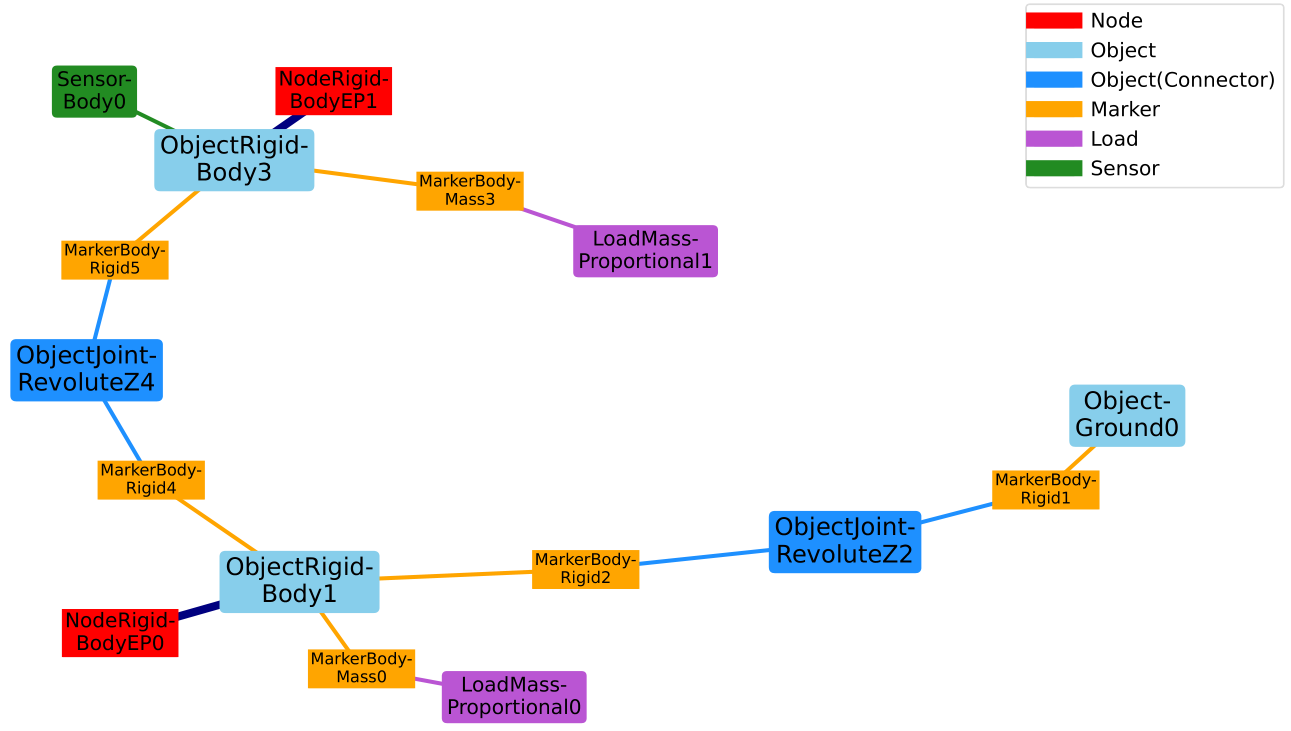
\includegraphics[width=0.9\textwidth]{figures/DrawSystemGraphExample}
  %\end{center}
  %\caption{System graph for rigid body tutorial (with option 3 for the first revolute joint). Numbers are always related to the node number, object number, etc.; note that colors are used to distinguish nodes, objects, markers, loads and sensors}
  %\label{fig_DrawSystemGraphExample}
%\end{figure}}
%\onlyRST{
%
%.. image:: docs/theDoc/figures/DrawSystemGraphExample.png
   %:width: 600
%
%}

\horizontalRuler\\
\noindent Before starting our simulation, we should adjust the solver parameters, especially the end time and the step size (no automatic step size for implicit solvers available!):
\pythonstyle\begin{lstlisting}
  simulationSettings = exu.SimulationSettings() #takes currently set values or default values

  tEnd = 4 #simulation time
  h = 1e-3 #step size
  simulationSettings.timeIntegration.numberOfSteps = int(tEnd/h)
  simulationSettings.timeIntegration.endTime = tEnd
  simulationSettings.timeIntegration.verboseMode = 1
  #simulationSettings.timeIntegration.simulateInRealtime = True
  simulationSettings.solutionSettings.solutionWritePeriod = 0.005 #store every 5 ms
\end{lstlisting}
The \texttt{verboseMode} tells the solver the amount of output during solving. Higher values (2, 3, ...) show residual vectors, jacobians, etc. for every time step, but slow down simulation significantly.
The option \texttt{simulateInRealtime} is used to view the model during simulation, while setting this false, 
the simulation finishes after fractions of a second. It should be set to false in general, 
while solution can be viewed using the \texttt{SolutionViewer()}.
With \texttt{solutionWritePeriod} you can adjust the frequency which is used to store the solution of the whole model, 
which may lead to very large files and may slow down simulation, but is used in the \texttt{SolutionViewer()} to reload the solution after simulation.

\noindent In order to improve visualization, there are hundreds of options, see Visualization settings in \refSection{sec:VisualizationSettingsMain}, some of them used here:
\pythonstyle\begin{lstlisting}
  SC.visualizationSettings.window.renderWindowSize = [1600,1200]
  SC.visualizationSettings.openGL.multiSampling = 4  #improved OpenGL rendering
  SC.visualizationSettings.general.autoFitScene = False

  SC.visualizationSettings.nodes.drawNodesAsPoint = False
  SC.visualizationSettings.nodes.showBasis = True #shows three RGB (=xyz) lines for node basis
\end{lstlisting}
The option \texttt{autoFitScene} is used in order to avoid zooming while loading the last saved render state, see below.

\noindent We can start the 3D visualization (Renderer) now:
\pythonstyle\begin{lstlisting}
  SC.renderer.Start()
\end{lstlisting}

\noindent In order to reload the model view of the last simulation (if there is any), we can use the following commands:
\pythonstyle\begin{lstlisting}
  if 'renderState' in exu.sys: #reload old view
      SC.renderer.SetState(exu.sys['renderState'])

  SC.renderer.DoIdleTasks()    #stop before simulating
\end{lstlisting}
the function \texttt{WaitForUserToContinue()} waits with simulation until we press SPACE bar. This allows us to make some pre-checks.

\noindent Finally, the \mybold{index 2} (velocity level) implicit time integration (simulation) is started with:
\pythonstyle\begin{lstlisting}
  mbs.SolveDynamic(simulationSettings = simulationSettings,
                   solverType = exu.DynamicSolverType.TrapezoidalIndex2)
\end{lstlisting}
This solver is used in the present example, but should be considered with care as it leads to (small) drift of position constraints, linearly increasing in time. Using sufficiently small time steps, this effect is often negligible on the advantage of having a \mybold{energy-conserving integrator} (guaranteed for linear systems, but very often also for the nonlinear multibody system). Due to the velocity level, the integrator is less sensitive to consistent initial conditions on position level and compatible to frequent step size changes, however, initial jumps in velocities may never damp out in undamped systems.

\noindent Alternatively, an \mybold{index 3} implicit time integration -- the generalized-$\alpha$ method -- is started with the default settings for \texttt{solverType}:
\pythonstyle\begin{lstlisting}
  mbs.SolveDynamic(simulationSettings = simulationSettings)
\end{lstlisting}
Note that the \mybold{generalized-$\alpha$ method} includes numerical damping (adjusted with the spectral radius) for stabilization of index 3 constraints. This leads to effects every time the integrator is (re-)started, e.g., when adapting time step sizes. For fixed step sizes, this is \mybold{the recommended integrator}.

\noindent After simulation, the library would immediately exit (and jump back to iPython or close the terminal window). In order to avoid this, we can use \texttt{WaitForRenderEngineStopFlag()} to wait until we press key 'Q'.
\pythonstyle\begin{lstlisting}
  SC.renderer.DoIdleTasks()   #stop before closing
  SC.renderer.Stop()          #safely close rendering window!
\end{lstlisting}
If you entered everything correctly, the render window should show a nice animation of the 3D double pendulum after pressing the SPACE key. 
If we do not stop the renderer (\texttt{SC.renderer.Stop()}), it will stay open for further simulations. However, it is safer to always close the renderer at the end.

\noindent As the simulation will run very fast, if you did not set \texttt{simulateInRealtime} to true. However, you can reload the stored solution and view the stored steps interactively:
\pythonstyle\begin{lstlisting}
  mbs.SolutionViewer()
  #alternatively, we could load solution from a file:
  #from exudyn.utilities import LoadSolutionFile
  #sol = LoadSolutionFile('coordinatesSolution.txt')
  #mbs.SolutionViewer(sol)
\end{lstlisting}

\noindent Finally, we can plot our sensor, drawing the y-component of the sensor (check out the many options in \texttt{PlotSensor(...)} to conveniently represent results!):
\pythonstyle\begin{lstlisting}
  mbs.PlotSensor(sensorNumbers=[sens1],components=[1],closeAll=True)
\end{lstlisting}

\noindent \mybold{Congratulations}! You completed the rigid body tutorial, which gives you the ability to model multibody systems. Note that much more complicated models are possible, including feedback control or flexible bodies, see the Examples!


%+++++++++++++++++++++++++++++++++++++++++++++++++++++++++++++++++++++++++++++++
%+++++++++++++++++++++++++++++++++++++++++++++++++++++++++++++++++++++++++++++++
\mysubsection{Flexible beams tutorial}
This tutorial briefly introduces two simple planar beams and how to work with them with utility functions.
The python source code of the beam tutorial can be found at:
\bi
  \item[] \texttt{main/pythonDev/Examples/beamTutorial.py}
\ei
The tutorial uses the GeometricallyExactBeam2D, which is a shear deformable Reissner-Timoshenko beam, and a thin cable ANCFCable2D, which represents a large deformation Bernoulli-Euler beam.

\noindent The model includes two highly flexible planar with length 2m, height 0.005m, width 0.01m, 
Young's modulus 1e9N/m$^2$ and density 2000kg/m$^3$.
The shear deformable beam is rigidly attached to ground and the cable is rigidly attached to a moving ground.

\noindent We first import necessary libraries and set up a mbs. Note that utilities also include pi, sin, cos and sqrt.
\pythonstyle\begin{lstlisting}
  import exudyn as exu
  from exudyn.utilities import *
  import numpy as np

  SC = exu.SystemContainer()
  mbs = SC.AddSystem()
\end{lstlisting}

\noindent We define a set of beam parameters, discretization and geometry for both beam models.
\pythonstyle\begin{lstlisting}
  numberOfElements = 16
  L = 2                     # length of pendulum 
  E=2e11                    # steel
  rho=7800                  # elastomer
  h=0.005                   # height of rectangular beam element in m
  b=0.01                    # width of rectangular beam element in m
  A=b*h                     # cross sectional area of beam element in m^2
  I=b*h**3/12               # second moment of area of beam element in m^4
  nu = 0.3                  # Poisson's ratio
      
  EI = E*I
  EA = E*A
  rhoA = rho*A
  rhoI = rho*I
  ks = 10*(1+nu)/(12+11*nu) # shear correction factor
  G = E/(2*(1+nu))          # shear modulus
  GA = ks*G*A               # shear stiffness of beam

  g = [0,-9.81,0]           # gravity vector

  positionOfNode0 = [0,0,0] # 3D vector
  positionOfNode1 = [L,0,0] # 3D vector
\end{lstlisting}

\noindent Build geometrically exact 2D beam template (Timoshenko-Reissner), which includes all parameters
In order to create beams, we usually need to create 2D rigid body nodes, 
create beam elements, add constraints and loads.

\noindent However, there is a utility function \texttt{GenerateStraightBeam(...)}, 
which conveniently does this for straight beams, including discretization, constraints and gravity.
First, we create a beam template, which includes all beam parameters (this could also be another beam type):
\pythonstyle\begin{lstlisting}
  beamTemplate = Beam2D(nodeNumbers = [-1,-1], #added later
                        physicsMassPerLength=rhoA,
                        physicsCrossSectionInertia=rhoI,
                        physicsBendingStiffness=EI,
                        physicsAxialStiffness=EA,
                        physicsShearStiffness=GA,
                        physicsBendingDamping=0.02*EI,
                        visualization=VObjectBeamGeometricallyExact2D(drawHeight = h))
\end{lstlisting}

\noindent Now we use this template and call \texttt{GenerateStraightBeam}, which takes the nodal positions,
calculates according beam element lengths from discretization and could add constraints,
if \texttt{fixedConstraintsNode0} or \texttt{fixedConstraintsNode1} are not \texttt{None}.
\pythonstyle\begin{lstlisting}
  beamData = GenerateStraightBeam(mbs, positionOfNode0, positionOfNode1, 
                                  numberOfElements, beamTemplate, gravity= g, 
                                  fixedConstraintsNode0=[1,1,1], 
                                  fixedConstraintsNode1=None)
\end{lstlisting}

\noindent We perform the same operations for ANCF cable elemente (Bernoulli-Euler),
but in this case, we do not add constraints:
\pythonstyle\begin{lstlisting}
  beamTemplate = Cable2D(nodeNumbers = [-1,-1], #added later
                         physicsMassPerLength=rhoA,
                         physicsBendingStiffness=EI,
                         physicsAxialStiffness=EA,
                         physicsBendingDamping=0.02*EI,
                         visualization=VCable2D(drawHeight = h))

  cableData = GenerateStraightBeam(mbs, positionOfNode0, positionOfNode1, 
                                   numberOfElements, beamTemplate, gravity= g, 
                                   fixedConstraintsNode0=None, 
                                   fixedConstraintsNode1=None)
\end{lstlisting}

\noindent Now, we create a ground object and markers to attach cable with generic joint
\pythonstyle\begin{lstlisting}
  oGround = mbs.CreateGround(referencePosition=[0,0,0])
  mGround = mbs.AddMarker(MarkerBodyRigid(bodyNumber=oGround, localPosition=[0,0,0]))
  mCable = mbs.AddMarker(MarkerNodeRigid(nodeNumber=cableData[0][0]))
\end{lstlisting}

\noindent As we like to move the cable relative to ground, we employ a simple 
user function which prescribes relative rotation and (corotated) translation in the joint:
\pythonstyle\begin{lstlisting}
  def UFoffset(mbs, t, itemNumber, offsetUserFunctionParameters):
      x = SmoothStep(t, 2, 4, 0, 0.5)   #translate in local joint coordinates
      phi = SmoothStep(t, 5, 10, 0, pi) #rotates frame of mGround
      return [x, 0,0,0,0,phi]

\end{lstlisting}

\noindent Finally, we add the rigid joint (2D displacements and rotation around Z fixed) as GenericJoint.
Note that for 2D objects, we may only fix $X$- and $Y$-translations, as well as the $Z$-rotation
\pythonstyle\begin{lstlisting}
  mbs.AddObject(GenericJoint(markerNumbers=[mGround, mCable],
                             constrainedAxes=[1,1,0, 0,0,1],
                             offsetUserFunction=UFoffset,
                             visualization=VGenericJoint(axesRadius=0.01,
                                                         axesLength=0.02)))
\end{lstlisting}

\noindent As in the previous example, we just need to assemble and set up simulation parameters:
\pythonstyle\begin{lstlisting}
  mbs.Assemble()

  simulationSettings = exu.SimulationSettings()
      
  tEnd = 10
  stepSize = 0.005
  simulationSettings.timeIntegration.numberOfSteps = int(tEnd/stepSize)
  simulationSettings.timeIntegration.endTime = tEnd
  simulationSettings.timeIntegration.verboseMode = 1
  simulationSettings.solutionSettings.solutionWritePeriod = 0.005
  simulationSettings.solutionSettings.writeSolutionToFile = True

  simulationSettings.linearSolverType = exu.LinearSolverType.EigenSparse
  simulationSettings.timeIntegration.newton.useModifiedNewton = True #for faster simulation

  ## add some visualization settings
  SC.visualizationSettings.nodes.defaultSize = 0.01
  SC.visualizationSettings.nodes.drawNodesAsPoint = False #show beam nodes
  SC.visualizationSettings.bodies.beams.crossSectionFilled = True
\end{lstlisting}

\noindent Now start the solver with visualization and run the solution viewer afterwards,
because simulation may be faster than you can follow:
\pythonstyle\begin{lstlisting}
  SC.renderer.Start()
  mbs.SolveDynamic(simulationSettings)
  SC.renderer.Stop()

  ## visualize computed solution:
  mbs.SolutionViewer()
\end{lstlisting}

\noindent The visualization window for the solution drawn at 6.5s is shown in \fig{fig_tutorial_beams}.
%
\LatexRSTfigure{figures/TutorialBeams}{fig_tutorial_beams}{15cm}{500}{Render window showing the deformed state of the two beams at 6.5s. The lower beam is fixed at the left end, while the upper beam's support is translated and rotated.}
%

\noindent This example should give you a good starting point to create beam models.
See further examples, and more advanced functions, e.g., to create curved beam or reeving systems.
There are also a sliding joint as well as axially moving beams and contact between beams and sheaves.

\noindent 3D beams are still under development and include less functionality. In case, send a request at the GitHub discussion or issues.

\clearpage
%+++++++++++++++++++++++++++++++++++++++++++++++++++++++++++++++++++++++++++++++
%+++++++++++++++++++++++++++++++++++++++++++++++++++++++++++++++++++++++++++++++
\mysubsection{Symbolic user function tutorial}

The following tutorial demonstrates the setup of a nonlinear oscillator with a mass point and a force user function, using a Cartesian spring damper defined by symbolic user functions.
\vspace{6pt}\\
First, we import the necessary libraries, create a system container and a main system:
\pythonstyle\begin{lstlisting}
  import exudyn as exu
  from exudyn.utilities import *  # includes itemInterface and rigidBodyUtilities
  import exudyn.graphics as graphics  # only import if it does not conflict
  SC = exu.SystemContainer()
  mbs = SC.AddSystem()
\end{lstlisting}
%
We set an abbreviation for the symbolic library for convenient access; 
often you can replace that with numpy:
\pythonstyle\begin{lstlisting}
  esym = exu.symbolic
\end{lstlisting}
%
Now, define the parameters for the linear spring-damper system:
\pythonstyle\begin{lstlisting}
  L = 0.5
  mass = 1.6
  k = 4000
  omega0 = 50  # sqrt(k / mass)
  dRel = 0.05
  d = dRel * 2 * omega0
  u0 = -0.08
  v0 = 1
  f = 80
\end{lstlisting}
%
Create the ground object and the mass point with initial conditions:
\pythonstyle\begin{lstlisting}
  objectGround = mbs.CreateGround(referencePosition=[0, 0, 0])
  massPoint = mbs.CreateMassPoint(referencePosition=[L, 0, 0],
                                  initialDisplacement=[u0, 0, 0],
                                  initialVelocity=[v0, 0, 0],
                                  physicsMass=mass)
\end{lstlisting}
%
Set up the Cartesian spring damper between the ground and the mass point, and apply an external force on the mass point:
\pythonstyle\begin{lstlisting}
  csd = mbs.CreateCartesianSpringDamper(bodyNumbers=[objectGround, massPoint],
                                        stiffness=[k, k, k],
                                        damping=[d, 0, 0],
                                        offset=[L, 0, 0])
  load = mbs.CreateForce(bodyNumber=massPoint, loadVector=[f, 0, 0])
\end{lstlisting}
%
Add a sensor to monitor the position of the mass point:
\pythonstyle\begin{lstlisting}
  sMass = mbs.AddSensor(SensorBody(bodyNumber=massPoint,
                                   storeInternal=True,
                                   outputVariableType=exu.OutputVariableType.Position))
\end{lstlisting}
%
Define a user function for the Cartesian spring damper, which may use Python or symbolic expressions:
\pythonstyle\begin{lstlisting}
  def springForceUserFunction(mbs, t, itemNumber, u, v, k, d, offset):
      return [0.5 * u[0]**2 * k[0] + esym.sign(v[0]) * 10, k[1] * u[1], k[2] * u[2]]
\end{lstlisting}
%
We assign \texttt{CSDuserFunction} to the Python user function. This is used if no symbolic user function is used:
\pythonstyle\begin{lstlisting}
  CSDuserFunction = springForceUserFunction
\end{lstlisting}
%
Up to now, everything looks like regular user functions. We now add an optional way to create a symbolic user function, which runs much faster in this case:
\pythonstyle\begin{lstlisting}
  doSymbolic = True
  if doSymbolic:
      CSDuserFunction = CreateSymbolicUserFunction(mbs, springForceUserFunction,
                                                   'springForceUserFunction', csd)
      # Check function:
      print('user function:\n', CSDuserFunction)
\end{lstlisting}
%
Set the user function to the object, assemble the system, and configure the simulation settings:
\pythonstyle\begin{lstlisting}
  mbs.SetObjectParameter(csd, 'springForceUserFunction', CSDuserFunction)
  mbs.Assemble()

  simulationSettings = exu.SimulationSettings()
  tEnd = 2
  steps = 200000
  simulationSettings.timeIntegration.numberOfSteps = steps
  simulationSettings.timeIntegration.endTime = tEnd
  simulationSettings.timeIntegration.verboseMode = 1
  simulationSettings.solutionSettings.writeSolutionToFile = False
  simulationSettings.solutionSettings.sensorsWritePeriod = 0.001
\end{lstlisting}
%
Finally, start the renderer and solver, then evaluate the solution:
\pythonstyle\begin{lstlisting}
  SC.renderer.Start()
  mbs.SolveDynamic(simulationSettings, solverType=exu.DynamicSolverType.ExplicitMidpoint)
  SC.renderer.Stop()  # safely close rendering window!
  n1 = mbs.GetObject(massPoint)['nodeNumber']
  u = mbs.GetNodeOutput(n1, exu.OutputVariableType.Position)
  print('u=', u)
  mbs.PlotSensor(sMass)
\end{lstlisting}
%
NOTE: this tutorial has been mostly created with ChatGPT-4, and curated hereafter!


%+++++++++++++++++++++++++++++++++++++++++++++++++++++++++++++++++++++++++++++++
%+++++++++++++++++++++++++++++++++++++++++++++++++++++++++++++++++++++++++++++++
\mysubsection{Flexible body -- FFRF tutorial}
The following tutorial includes flexible bodies, using the floating frame of reference formulation (FFRF), 
including Netgen and NGsolve for mesh and finite element data generation and uses modal reduction for simulation.
The tutorial will set up a body with Hurty-Craig-Bampton modes, giving a simple flexible pendulum meshed hinged with a revolute joint.
\LatexRSTfigure{figures/TutorialFFRFpendulum}{fig_tutorial_FFRFpendulum}{12cm}{400}{Screen shot of pendulum modeled with floating frame of reference formulation, using HCB modes, and meshed with Netgen.}
%
\vspace{6pt}\\
We import the exudyn library, utilities, and other necessary modules:
\pythonstyle\begin{lstlisting}
    import exudyn as exu
    from exudyn.utilities import *  # includes itemInterface and rigidBodyUtilities
    import exudyn.graphics as graphics  # only import if it does not conflict
    from exudyn.FEM import *
    import numpy as np
    import time
    import ngsolve as ngs
    from netgen.meshing import *
    from netgen.csg import *
\end{lstlisting}
%
Next, we need a \texttt{SystemContainer}, which contains all computable systems and adds a new MainSystem \texttt{mbs}:
\pythonstyle\begin{lstlisting}
    SC = exu.SystemContainer()
    mbs = SC.AddSystem()
\end{lstlisting}
%
Define the parameters and setup the Netgen mesh, using Netgen's CSG geometry. We create a simple brick in order to simplify the application of boundary interfaces and joints:
\pythonstyle\begin{lstlisting}
    useGraphics = True
    fileName = 'testData/netgenBrick'  # for load/save of FEM data
    
    a = 0.025  # height/width of beam
    b = a
    h = 0.5 * a 
    L = 1     # Length of beam
    nModes = 8

    rho = 1000
    Emodulus = 1e7 * 10
    nu = 0.3
    meshCreated = False
    meshOrder = 1  # use order 2 for higher accuracy, but more unknowns

    geo = CSGeometry()
    block = OrthoBrick(Pnt(0, -a, -b), Pnt(L, a, b))
    geo.Add(block)
    mesh = ngs.Mesh(geo.GenerateMesh(maxh=h))
    mesh.Curve(1)
\end{lstlisting}
%
When creating the geometry and mesh, we sometimes would like to verify that with Netgen's GUI. 
In Jupyter, this works smoother with \texttt{webgui\_jupyter\_widgets} -- see the Netgen documention. Here we use a simple loop, which has to set \texttt{True} if visualization shall run:
\pythonstyle\begin{lstlisting}
    if False:  # set this to true, if you want to visualize the mesh inside netgen/ngsolve
        import netgen.gui
        ngs.Draw(mesh)
        for i in range(10000000):
            netgen.Redraw()  # this makes the window interactive
            time.sleep(0.05)
\end{lstlisting}
%
Use the FEM interface to import the FEM model and create the FFRF reduced-order data stored in fem.
Note that on importing the FEM structure from NGsolve (the FEM-module and solver of Netgen), we 
have to specify the mechanical properties related to the mesh:
\pythonstyle\begin{lstlisting}
    fem = FEMinterface()
    [bfM, bfK, fes] = fem.ImportMeshFromNGsolve(mesh, density=rho, 
                                                youngsModulus=Emodulus, 
                                                poissonsRatio=nu,
                                                meshOrder=meshOrder)
                                                
\end{lstlisting}
%
We could now just compute eigenmodes of the free bodies. However, as mentioned in the theory part, they do not respect boundary conditions and lead to low accuracy. Therefore, we use Hurty-Craig-Bampton modes.
For them, we have to define boundary interfaces given as lists of node numbers as well as weights.
We can use convenient functions from the \texttt{FEMinterface} class to retrieve nodes from planar or cylindrical surfaces (or we may define them in the finite element model ourselves):
\pythonstyle\begin{lstlisting}
    pLeft = [0, -a, -b]
    pRight = [L, -a, -b]
    nTip = fem.GetNodeAtPoint(pRight) #for sensor
    nodesLeftPlane = fem.GetNodesInPlane(pLeft, [-1, 0, 0])
    weightsLeftPlane = fem.GetNodeWeightsFromSurfaceAreas(nodesLeftPlane)
    nodesRightPlane = fem.GetNodesInPlane(pRight, [-1, 0, 0])
    weightsRightPlane = fem.GetNodeWeightsFromSurfaceAreas(nodesRightPlane)
\end{lstlisting}
%
We define a list of boundaries, which are then passed to the function which computes modes.
Note that by default the first boundary modes are eliminated as they are fixed to the reference frame
of the FFRF object:
\pythonstyle\begin{lstlisting}
    boundaryList = [nodesLeftPlane]

    print("nNodes=", fem.NumberOfNodes())
    print("compute HCB modes... ")
    start_time = time.time()
    fem.ComputeHurtyCraigBamptonModes(boundaryNodesList=boundaryList, 
                                      nEigenModes=nModes, 
                                      useSparseSolver=True,
                                      computationMode=HCBstaticModeSelection.RBE2)
    print("HCB modes needed %.3f seconds" % (time.time() - start_time))
\end{lstlisting}
%
Compute stress modes for postprocessing, which is not needed for simulation, but useful for postprocessing:
\pythonstyle\begin{lstlisting}
    if True:
        mat = KirchhoffMaterial(Emodulus, nu, rho)
        varType = exu.OutputVariableType.StressLocal
        print("ComputePostProcessingModes ... (may take a while)")
        start_time = time.time()
        fem.ComputePostProcessingModesNGsolve(fes, material=mat,
                                              outputVariableType=varType)
        print("   ... needed %.3f seconds" % (time.time() - start_time))
        SC.visualizationSettings.contour.reduceRange = False
        SC.visualizationSettings.contour.outputVariable = varType
        SC.visualizationSettings.contour.outputVariableComponent = 0  # x-component
    else:
        SC.visualizationSettings.contour.outputVariable = exu.OutputVariableType.DisplacementLocal
        SC.visualizationSettings.contour.outputVariableComponent = 1 
\end{lstlisting}
%
Having all data prepared now, we create the CMS element which is an object added then to \texttt{mbs}:
\pythonstyle\begin{lstlisting}
    print("create CMS element ...")
    cms = ObjectFFRFreducedOrderInterface(fem)
    objFFRF = cms.AddObjectFFRFreducedOrder(mbs, positionRef=[0, 0, 0], 
                                            initialVelocity=[0, 0, 0], 
                                            initialAngularVelocity=[0, 0, 0],
                                            gravity=[0, -9.81, 0],
                                            color=[0.1, 0.9, 0.1, 1.])
\end{lstlisting}
%
Add markers and revolute joint, using a superelement marker:
\pythonstyle\begin{lstlisting}
    nodeDrawSize = 0.0025  # for joint drawing

    mRB = mbs.AddMarker(MarkerNodeRigid(nodeNumber=objFFRF['nRigidBody']))
    oGround = mbs.AddObject(ObjectGround(referencePosition=[0, 0, 0]))
    leftMidPoint = [0, 0, 0]
    mGround = mbs.AddMarker(MarkerBodyRigid(bodyNumber=oGround, localPosition=leftMidPoint))
    mLeft = mbs.AddMarker(MarkerSuperElementRigid(bodyNumber=objFFRF['oFFRFreducedOrder'], 
                                                  meshNodeNumbers=np.array(nodesLeftPlane), 
                                                  weightingFactors=weightsLeftPlane))
    mbs.AddObject(GenericJoint(markerNumbers=[mGround, mLeft], 
                               constrainedAxes=[1, 1, 1, 1, 1, 1 * 0],
                               visualization=VGenericJoint(axesRadius=0.1 * a, axesLength=0.1 * a)))
\end{lstlisting}
Note that the marker is using weights, which are needed to compute accurate average (midpoint) positions from the non-uniform triangular surface mesh.

\noindent Now we finally add a sensor and assemble the system:
\pythonstyle\begin{lstlisting}
    fileDir = 'solution/'
    sensTipDispl = mbs.AddSensor(SensorSuperElement(bodyNumber=objFFRF['oFFRFreducedOrder'], 
                                                    meshNodeNumber=nTip, 
                                                    fileName=fileDir + 'nMidDisplacementCMS' + str(nModes) + 'Test.txt', 
                                                    outputVariableType=exu.OutputVariableType.Displacement))

    mbs.Assemble()
\end{lstlisting}
%
Set simulation settings and run the simulation:
\pythonstyle\begin{lstlisting}
    simulationSettings = exu.SimulationSettings()

    SC.visualizationSettings.nodes.defaultSize = nodeDrawSize
    SC.visualizationSettings.nodes.drawNodesAsPoint = False
    SC.visualizationSettings.connectors.defaultSize = 2 * nodeDrawSize
    SC.visualizationSettings.nodes.show = False
    SC.visualizationSettings.sensors.show = True
    SC.visualizationSettings.sensors.defaultSize = 0.01
    SC.visualizationSettings.markers.show = False
    SC.visualizationSettings.loads.drawSimplified = False

    h = 1e-3
    tEnd = 4

    simulationSettings.timeIntegration.numberOfSteps = int(tEnd / h)
    simulationSettings.timeIntegration.endTime = tEnd
    simulationSettings.timeIntegration.verboseMode = 1
    simulationSettings.timeIntegration.newton.useModifiedNewton = True
    simulationSettings.solutionSettings.sensorsWritePeriod = h
    simulationSettings.timeIntegration.generalizedAlpha.spectralRadius = 0.8
    simulationSettings.displayComputationTime = True

    mbs.SolveDynamic(simulationSettings=simulationSettings)

    uTip = mbs.GetSensorValues(sensTipDispl)[1]
    print("nModes=", nModes, ", tip displacement=", uTip)

    mbs.SolutionViewer()
\end{lstlisting}
When the solution viewer starts, it should show the stresses in a flexible swinging pendulum, see \fig{fig_tutorial_FFRFpendulum}.


NOTE: this tutorial has been mostly created with ChatGPT-4, and curated hereafter!

}

%+++++++++++++++++++++++++++++++++++++++++++++++++++++++++++++++++++++++++++++++
%+++++++++++++++++++++++++++++++++++++++++++++++++++++++++++++++++++++++++++++++
%\mysection{Python-C++ command interface} \label{sec:PCpp:command:interface}
%This chapter lists the basic interface functions which can be used to set up a \codeName\ model in Python.
%
%\mysubsection{General information on Python interface}
%\label{sec:generalPythonInterface}
%%
%To import the module, just include the \codeName\ module in Python (for compatibility with examples and other users, we recommend to use the '\texttt{exu}' abbreviation throughout):
%\bi
  %\item[] \texttt{import exudyn as exu}
%\ei
%In addition, you may work with a convenient interface for your items, therefore also always include the line
%\bi
  %\item[] \texttt{from exudyn.itemInterface import *}
%\ei
%Everything you work with is provided by the class \texttt{SystemContainer}, except for some very basic system functionality (which is inside the \codeName\ module).
%
%You can create a new \texttt{SystemContainer}, which is a class that is initialized by assigning a system container to a variable, usually denoted as 'SC':
%\bi
  %\item[] \texttt{SC = exu.SystemContainer()}
%\ei
%Note that creating a second \texttt{exu.SystemContainer()} will be independent of \texttt{SC} and therefore usually makes no sense.
%
%Furthermore, there are a couple of commands available directly in the \codeName\ module, given in the following subsections.
%Regarding the {\bf (basic) module access}, functions are related to the '\texttt{exudyn = exu}' module, see these examples:
%\begin{lstlisting}[language=Python, firstnumber=14]
  %import exudyn as exu
  %from exudyn.itemInterface import *
  %SC = exu.SystemContainer()
  %exu.InfoStat() #prints some statistics if available
  %exu.Go() #creates a systemcontainer and main system
  %nInvalid = exu.InvalidIndex() #the invalid index, depends on architecture and version
%\end{lstlisting} \vspace{12pt}
%
%Understanding the usage of functions for python object '\texttt{SystemContainer}' provided by \codeName, the following examples might help:
%\begin{lstlisting}[language=Python, firstnumber=14]
  %import exudyn as exu
  %from exudyn.itemInterface import *
  %SC = exu.SystemContainer()
  %mbs = SC.AddSystem()
  %nSys = SC.NumberOfSystems()
  %print(nSys)
  %SC.Reset()
%\end{lstlisting} \vspace{12pt}
%%
%If you run a parameter variation (check \texttt{Examples/parameterVariationExample.py}), you may delete the created \texttt{MainSystem} \texttt{mbs} and the \texttt{SystemContainer} \texttt{SC} before creating new instances in order to avoid memory growth.
%
%\mysubsubsection{Item index}
%\label{sec:itemIndex}
%Many functions will work with node numbers ('\texttt{NodeIndex}'), object numbers ('\texttt{ObjectIndex}'), marker numbers ('\texttt{MarkerIndex}') and others. These numbers are special objects, which have been introduced in order to avoid mixing up, e.g., node and object numbers.
%For example, the command \texttt{mbs.AddNode(...)} returns a \texttt{NodeIndex}. For these indices, the following rules apply:
%\bi
	%\item \texttt{mbs.Add[Node|Object|...](...)} returns a specific \texttt{NodeIndex}, \texttt{ObjectIndex}, ...
	%\item You can create any item index, e.g., using \texttt{ni = NodeIndex(42)} or \texttt{oi = ObjectIndex(42)}
	%\item You can convert any item index, e.g., NodeIndex \texttt{ni} into an integer number using \texttt{int(ni)} of \texttt{no.GetIndex()}
	%\item Still, you can use integers as initialization for item numbers, e.g., \\
	      %\texttt{mbs.AddObject(MassPoint(nodeNumber=13, ...))}\\
				%However, it must be a pure integer type.
	%\item You can also print item indices, e.g., \texttt{print(ni)} as it converts to string by default
	%\item If you are unsure about the type of an index, use \texttt{ni.GetTypeString()} to show the index type
%\ei

%+++++++++++++++++++++++++++++++++++++
\iftoggle{compileAll}
{
%solver
%+++++++++++++++++++++++++++++++++++++++++++++++++++++++++++++++++++++++++++++
%+++++++++++++++++++++++++++++++++++++++++++++++++++++++++++++++++++++++++++++
\mysectionlabel{Notation}{sec:generalnotation}
%
The notation is used to explain:
\bi
  \item typical symbols in equations and formulas (e.g., $q$)
  \item common types used as parameters in items (e.g., \texttt{PInt})
  \item typical annotation of equations (or parts of it) and symbols (e.g., \texttt{ODE2})
\ei

%+++++++++++++++++++++++++++++++++++++++++++++++++++++++++++++++++++++++++++++++++++++++++++
%+++++++++++++++++++++++++++++++++++++++++++++++++++++++++++++++++++++++++++++++++++++++++++
\mysubsubsectionlabel{Common types}{sec:typesDescriptions}
%
Common types are especially used in the definition of items. 
These types indicate how they need to be set (e.g., a \texttt{Vector3D} is set as a list of 3 floats or as a numpy array with 3 floats), 
and they usually include some range or size check (e.g., \texttt{PReal} is checked for being positive and non-zero):
\bi
  \item \texttt{float} $\ldots$ a single-precision floating point number (note: in Python, '\texttt{float}' is used also for double precision numbers; in EXUDYN, internally floats are single precision numbers especially for graphics objects and OpenGL)
  \item \texttt{Real} $\ldots$ a double-precision floating point number (note: in Python this is also of type '\texttt{float}')
  \item \texttt{UReal} $\ldots$ same as \texttt{Real}, but may not be negative
  \item \texttt{PReal} $\ldots$ same as \texttt{Real}, but must be positive, non-zero (e.g., step size may never be zero)
  \item \texttt{Index} $\ldots$ deprecated, represents unsined integer, \texttt{UInt}
  \item \texttt{Int} $\ldots$ a (signed) integer number, which converts to '\texttt{int}' in Python, '\texttt{int}' in C++
  \item \texttt{UInt} $\ldots$ an unsigned integer number, which converts to '\texttt{int}' in Python
  \item \texttt{PInt} $\ldots$ an positive integer number (> 0), which converts to '\texttt{int}' in Python
%
  \item \texttt{NodeIndex, MarkerIndex, ...} $\ldots$ a special (non-negative) integer type to represent indices of nodes, markers, ...; specifically, an unintentional conversion from one index type to the other is not possible (e.g., to convert \texttt{NodeIndex} to \texttt{MarkerIndex}); see \refSection{sec:itemIndex}
  \item \texttt{String} $\ldots$ a string
  \item \texttt{ArrayIndex} $\ldots$ a list of integer numbers (either list or in some cases \texttt{numpy} arrays may be allowed)
  \item \texttt{ArrayNodeIndex} $\ldots$ a list of node indices
  \item \texttt{Bool} $\ldots$ a boolean parameter: either \texttt{True} or \texttt{False} ('\texttt{bool}' in Python)
  \item \texttt{VObjectMassPoint}, \texttt{VObjectRigidBody}, \texttt{VObjectGround}, etc.  $\ldots$ represents the visualization object of the underlying object; 'V' is put in front of object name
  \item \texttt{BodyGraphicsData} $\ldots$ see \refSection{sec:graphicsData}
%
  \item \texttt{Vector2D} $\ldots$ a list or \texttt{numpy} array of 2 real numbers
  \item \texttt{Vector3D} $\ldots$ a list or \texttt{numpy} array of 3 real numbers
  \item \texttt{Vector'X'D} $\ldots$ a list or \texttt{numpy} array of 'X' real numbers
  \item \texttt{Float4} $\ldots$ a list of 4 float numbers
  \item \texttt{Vector} $\ldots$ a list or \texttt{numpy} array of real numbers (length given by according object)
  \item \texttt{NumpyVector} $\ldots$ a 1D \texttt{numpy} array with real numbers (size given by according object); similar as Vector, but not accepting list
%
  \item \texttt{Matrix3D} $\ldots$ a list of lists or \texttt{numpy} array with $3 \times 3$ real numbers
  \item \texttt{Matrix6D} $\ldots$ a list of lists or \texttt{numpy} array with $6 \times 6$ real numbers
  \item \texttt{NumpyMatrix} $\ldots$ a 2D \texttt{numpy} array (matrix) with real numbers (size given by according object)
  \item \texttt{NumpyMatrixI} $\ldots$ a 2D \texttt{numpy} array (matrix) with integer numbers (size given by according object)
  \item \texttt{MatrixContainer} $\ldots$ a versatile representation for dense and sparse matrices, see \refSection{sec:MatrixContainer}
%
  \item \texttt{PyFunctionGraphicsData} $\ldots$ a user function providing GraphicsData, see the user function description of the according object
  \item \texttt{PyFunctionMbsScalar...} $\ldots$ a user function for the according object; the name is chosen according to the interface (arguments containing scalars, vectors, etc.) and is only used internally for code generation; see the according user function description
\ei

%
\mysubsubsection{States and coordinate attributes}
The following subscripts are used to define configurations of a quantity, e.g., for a vector of displacement coordinates $\qv$:
\bi
  \item $\qv\cConfig \ldots$ $\qv$ in any configuration
  \item $\qv\cRef \ldots$ $\qv$ in reference configuration, e.g., reference coordinates: $\cv\cRef$
  \item $\qv\cIni \ldots$ $\qv$ in initial configuration, e.g., initial displacements: $\uv\cIni$
  \item $\qv\cCur \ldots$ $\qv$ in current configuration
  \item $\qv\cVis \ldots$ $\qv$ in visualization configuration
  \item $\qv\cSOS \ldots$ $\qv$ in start of step configuration
\ei
As written in the introduction, the coordinates are attributed to certain types of equations and therefore, the following attributes are used (usually as subscript, e.g., $\qv_{ODE2}$):
\ignoreRST{
\bi
  \item \hacs{ODE2} $\ldots$ \acl{ODE2} (coordinates)
  \item \hacs{ODE1} $\ldots$ \acl{ODE1} (coordinates)
  \item \hacs{AE} $\ldots$ \acl{AE} (coordinates)
  \item Data $\ldots$ data coordinates (history variables)
\ei}
\onlyRST{

 + \hacs{ODE2}, \hacs{ODE1}, \hacs{AE}, Data : These attributes refer to these types of equations or coordinates (click to see explanation)

}
Time is usually defined as 'time' or $t$.
The cross product or vector product '$\times$' is often replaced by the skew symmetric matrix using the tilde '$\tilde{\;\;}$' symbol,
\be
  \av \times \bv = \tilde \av \, \bv = -\tilde \bv \, \av \eqComma
\ee
in which $\tilde{\;\;}$ transforms a vector $\av$ into a skew-symmetric matrix $\tilde \av$.
If the components of $\av$ are defined as $\av = \vrRow{a_0}{a_1}{a_2}\tp$, then the skew-symmetric matrix reads
\be
  \tilde \av = \mr{0}{-a_2}{a_1} {a_2}{0}{-a_0} {-a_1}{a_0}{0} \eqDot
\ee
The inverse operation is denoted as $\vec$, resulting in $\vec(\tilde \av) = \av$.

For the length of a vector we often use the abbreviation 
\be \label{eq:definition:length}
  \Vert \av \Vert = \sqrt{\av^T \av} \eqDot
\ee

A vector $\av=[x,\, y,\, z]\tp$ can be transformed into a diagonal matrix, e.g.,
\be
  \Am = \diag(\av) = \mr{x}{0}{0} {0}{y}{0} {0}{0}{z} 
\ee
%
%+++++++++++++++++++++++++++++++++++++++++++++++++++++++++++++++++++++++++++++++++++++++++++
\mysubsubsectionlabel{Symbols in item equations}{sec:symbolsItems}
\noindent The following tables contains the common notation
General \mybold{coordinates} are: \vspace{-12pt}
%
\startGenericTable{| p{5cm} | p{5cm} | p{6cm} |}
\rowTableThree{\mybold{python name (or description)}}{\mybold{symbol}}{\mybold{description} }
\rowTableThree{displacement coordinates (\hac{ODE2})}{$\qv = [q_0,\, \ldots,\, q_n]\tp$}{vector of $n$ displacement based coordinates in any configuration; used for second order differential equations }
\rowTableThree{rotation coordinates (\hac{ODE2})}{$\tpsi = [\psi_0,\, \ldots,\, \psi_\eta]\tp$}{vector of $\eta$ \mybold{rotation based coordinates} in any configuration; these coordinates are added to reference rotation parameters to provide the current rotation parameters; used for second order differential equations }
\rowTableThree{coordinates (\hac{ODE1})}{$\yv = [y_0,\, \ldots,\, y_n]\tp$}{vector of $n$ coordinates for first order ordinary differential equations (\hac{ODE1}) in any configuration }
\rowTableThree{algebraic coordinates}{$\zv = [z_0,\, \ldots,\, z_m]\tp$}{vector of $m$ algebraic coordinates if not Lagrange multipliers in any configuration }
\rowTableThree{Lagrange multipliers}{$\tlambda = [\lambda_0,\, \ldots,\, \lambda_m]\tp$}{vector of $m$ Lagrange multipliers (=algebraic coordinates) in any configuration }
\rowTableThree{data coordinates}{$\xv = [x_0,\, \ldots,\, x_l]\tp$}{vector of $l$ data coordinates in any configuration }
\finishTable
%+++++++++++++++++++++++++++++++++++++++++++++++++++

The following parameters represent possible \mybold{OutputVariable} (list is not complete): \vspace{-12pt}
\startGenericTable{| p{5cm} | p{5cm} | p{6cm} |}
\rowTableThree{\mybold{python name}}{\mybold{symbol}}{\mybold{description} }
\rowTableThree{Coordinate}{$\cv = [c_0,\, \ldots,\, c_n]\tp$}{coordinate vector with $n$ generalized coordinates $c_i$ in any configuration; the letter $c$ is used both for \hac{ODE1} and \hac{ODE2} coordinates }
\rowTableThree{Coordinate\_t}{$\dot \cv = [c_0,\, \ldots,\, c_n]\tp$}{time derivative of coordinate vector }
\rowTableThree{Displacement}{$\LU{0}{\uv} = [u_0,\, u_1,\, u_2]\tp$}{global displacement vector with 3 displacement coordinates $u_i$ in any configuration; in 1D or 2D objects, some of there coordinates may be zero }
\rowTableThree{Rotation}{$[\varphi_0,\,\varphi_1,\,\varphi_2]\tp\cConfig$}{vector with 3 components of the Euler angles in xyz-sequence ($\LU{0b}{\Rot}\cConfig=:\Rot_0(\varphi_0) \cdot \Rot_1(\varphi_1) \cdot \Rot_2(\varphi_2)$), recomputed from rotation matrix }
\rowTableThree{Rotation (alt.)}{$\ttheta = [\theta_0,\, \ldots,\, \theta_n]\tp$}{vector of \mybold{rotation parameters} (e.g., Euler parameters, Tait Bryan angles, ...) with $n$ coordinates $\theta_i$ in any configuration }
\rowTableThree{Identity matrix}{$\Im = \mr{1}{0}{0} {0}{\ddots}{0} {0}{0}{1}$}{the identity matrix, very often $\Im = \ImThree$, the $3 \times 3$ identity matrix }
\rowTableThree{Identity transformation}{$\LU{0b}{\ImThree} = \ImThree$}{converts body-fixed into global coordinates, e.g., $\LU{0}{\xv} = \LU{0b}{\ImThree} \LU{b}{\xv}$, thus resulting in $\LU{0}{\xv} = \LU{b}{\xv}$ in this case }
\rowTableThree{RotationMatrix}{$\LU{0b}{\Rot} = \mr{A_{00}}{A_{01}}{A_{02}} {A_{10}}{A_{11}}{A_{12}} {A_{20}}{A_{21}}{A_{22}}$}{a 3D rotation matrix, which transforms local (e.g., body $b$) to global coordinates (0): $\LU{0}{\xv} = \LU{0b}{\Rot} \LU{b}{\xv}$ }
\rowTableThree{RotationMatrixX}{$\LU{01}{\Rot_0(\theta_0)} = \mr{1}{0}{0} {0}{\cos(\theta_0)}{-\sin(\theta_0)} {0}{\sin(\theta_0)}{\cos(\theta_0)}$}{rotation matrix for rotation around $X$ axis (axis 0), transforming a vector from frame 1 to frame 0 }
\rowTableThree{RotationMatrixY}{$\LU{01}{\Rot_1(\theta_1)} = \mr{\cos(\theta_1)}{0}{\sin(\theta_1)} {0}{1}{0} {-\sin(\theta_1)}{0}{\cos(\theta_1)}$}{rotation matrix for rotation around $Y$ axis (axis 1), transforming a vector from frame 1 to frame 0 }
\rowTableThree{RotationMatrixZ}{$\LU{01}{\Rot_2(\theta_2)} = \mr{\cos(\theta_2)}{-\sin(\theta_2)}{0} {\sin(\theta_2)}{\cos(\theta_2)}{0} {0}{0}{1}$}{rotation matrix for rotation around $Z$ axis (axis 2), transforming a vector from frame 1 to frame 0 }
\rowTableThree{Position}{$\LU{0}{\pv} = [p_0,\, p_1,\, p_2]\tp$}{global position vector with 3 position coordinates $p_i$ in any configuration }
\rowTableThree{Velocity}{$\LU{0}{\vv} = \LU{0}{\dot \uv} = [v_0,\, v_1,\, v_2]\tp$}{global velocity vector with 3 displacement coordinates $v_i$ in any configuration }
\rowTableThree{AngularVelocity}{$\LU{0}{\tomega} = [\omega_0,\, \ldots,\, \omega_2]\tp$}{global angular velocity vector with $3$ coordinates $\omega_i$ in any configuration }
\rowTableThree{Acceleration}{$\LU{0}{\av} = \LU{0}{\ddot \uv} = [a_0,\, a_1,\, a_2]\tp$}{global acceleration vector with 3 displacement coordinates $a_i$ in any configuration }
\rowTableThree{AngularAcceleration}{$\LU{0}{\talpha} = \LU{0}{\dot \tomega} = [\alpha_0,\, \ldots,\, \alpha_2]\tp$}{global angular acceleration vector with $3$ coordinates $\alpha_i$ in any configuration }
\rowTableThree{VelocityLocal}{$\LU{b}{\vv} = [v_0,\, v_1,\, v_2]\tp$}{local (body-fixed) velocity vector with 3 displacement coordinates $v_i$ in any configuration }
\rowTableThree{AngularVelocityLocal}{$\LU{b}{\tomega} = [\omega_0,\, \ldots,\, \omega_2]\tp$}{local (body-fixed) angular velocity vector with $3$ coordinates $\omega_i$ in any configuration }
\rowTableThree{Force}{$\LU{0}{\fv} = [f_0,\, \ldots,\, f_2]\tp$}{vector of $3$ force components in global coordinates }
\rowTableThree{Torque}{$\LU{0}{\ttau} = [\tau_0,\, \ldots,\, \tau_2]\tp$}{vector of $3$ torque components in global coordinates }
\finishTable
%+++++++++++++++++++++++++++++++++++++++++++++++++++

The following table collects some typical \mybold{input parameters} for nodes, objects and markers: \vspace{-12pt}
\startGenericTable{| p{5cm} | p{5cm} | p{6cm} |}
\rowTableThree{\mybold{python name}}{\mybold{symbol}}{\mybold{description} }
\rowTableThree{referenceCoordinates}{$\cv\cRef = [c_0,\, \ldots,\, c_n]\cRef\tp = [c_{\mathrm{Ref},0},\, \ldots,\, c_{\mathrm{Ref},n}]\cRef\tp$}{$n$ coordinates of reference configuration (can usually be set at initialization of nodes) }
\rowTableThree{initialCoordinates}{$\cv\cIni$}{initial coordinates with generalized or mixed displacement/rotation quantities (can usually be set at initialization of nodes) }
\rowTableThree{reference point}{$\pRefG = [r_0,\, r_1,\, r_2]\tp$}{reference point of body, e.g., for rigid bodies or \hac{FFRF} bodies, in any configuration; NOTE: for ANCF elements, $\pRefG$ is used for the position vector to the beam centerline }
\rowTableThree{localPosition}{$\pLocB = [\LUR{b}{b}{0},\, \LUR{b}{b}{1},\, \LUR{b}{b}{2}]\tp$}{local (body-fixed) position vector with 3 position coordinates $b_i$ in any configuration, measured relative to reference point; NOTE: for rigid bodies, $\LU{0}{\pv} = \pRefG + \LU{0b}{\Rot} \pLocB$; localPosition is used for definition of body-fixed local position of markers, sensors, COM, etc. }
\finishTable

%\mysubsectionlabel{Notation for equations of motion}
%
\ignoreRST{\mysubsectionlabel{\hac{LHS}--\hac{RHS} naming conventions in EXUDYN}{sec:equationLHSRHS}}
\onlyRST{\mysubsectionlabel{LHS-RHS naming conventions in EXUDYN}{sec:equationLHSRHS}}
The general idea of the \codeName\ is to have objects, which provide equations (\hac{ODE2}, \hac{ODE1}, \hac{AE}).
The solver then assembles these equations and solves the static or dynamic problem.
The system structure and solver are similar but much more advanced and modular as earlier solvers by the main developer \cite{GerstmayrStangl2004,Gerstmayr2009,GerstmayrEtAl2013}.

Functions and variables contain the abbreviations \hac{LHS} and \hac{RHS}, sometimes lower-case, in order
to distinguish if terms are computed at the \hac{LHS} or \hac{RHS}.

The objects have the following \hac{LHS}--\hac{RHS} conventions:
\bi
  \item the acceleration term, e.g., $m \cdot \ddot q$ is always positive on the \hac{LHS}
  \item objects, connectors, etc., use \hac{LHS} conventions for most terms: mass, stiffness matrix, elastic forces, damping, etc., are computed at \hac{LHS} of the object equation
  \item object forces are written at the \hac{RHS} of the object equation
  \item in case of constraint or connector equations, there is no \hac{LHS} or \hac{RHS}, as there is no acceleration term. 
\ei
Therefore, the computation function evaluates the term as given in the description of the object, adding it to the \hac{LHS}.
Object equations may read, e.g., for one coordinate $q$, mass $m$, damping coefficient $d$, stiffness $k$ and applied force $f$,
\be
  \underbrace{m \cdot \ddot q + d \cdot \dot q + k \cdot q}_{LHS} = \underbrace{f}_{RHS}
\ee 
In this case, the C++ function \texttt{ComputeODE2LHS(const Vector\& ode2Lhs)} will compute the term
$d \cdot \dot q + k \cdot q$ with positive sign. Note that the acceleration term $m \cdot \ddot q$ is computed separately, as it 
is computed from mass matrix and acceleration.

However, system quantities (e.g.\ within the solver) are always written on \hac{RHS}\footnote{except for the acceleration $\times$ mass matrix and constraint reaction forces, see \eq{eq_system_EOM}}: 
\be 
  \underbrace{M_{sys} \cdot \ddot q_{sys}}_{LHS} = \underbrace{f_{sys}}_{RHS} \,.
\ee
In the case of the object equation
\be
  m \cdot \ddot q + d \cdot \dot q + k \cdot q = f \, ,
\ee 
the \hac{RHS} term becomes $f_{sys} = -(d \cdot \dot q + k \cdot q) + f $ and it is computed by the C++ function \texttt{ComputeSystemODE2RHS}.
%
This means, that during computation, terms which appear at the \hac{LHS} of the object are transferred to the \hac{RHS} of the system equation.
This enables a simpler setup of equations for the solver.
%
\mysubsection{System assembly}
Assembling equations of motion is done within the C++ class \texttt{CSystem}, see the file \texttt{CSystem.cpp}.
The general idea is to assemble, i.e.\ to sum up, (parts of) residuals attributed by different objects. The summation process is based on coordinate indices to which the single equations belong to.
Let's assume that we have two simple \texttt{ObjectMass1D} objects, with object indices $o0$ and $o1$ and having mass $m_0$ and $m_1$. They are connected to nodes of type \texttt{Node1D} $n0$ and $n1$, with global coordinate indices $c0$ and $c1$.
The partial object residuals, which are fully independent equations, read
\bea
  m_0 \cdot \ddot q_{c0} &=& RHS_{c0} \eqComma \\
  m_1 \cdot \ddot q_{c1} &=& RHS_{c1} \eqComma
\eea
where $RHS_{c0}$ and $RHS_{c1}$ the right-hand-side of the respective equations/coordinates. They represent forces, e.g., from \texttt{LoadCoordinate} items (which directly are applied to coordinates of nodes), say $f_{c0}$ and $f_{c1}$, that are in case also summed up on the right hand side.
Let us for now assume that 
\be
  RHS_{c0} = f_{c0} \quad \mathrm{and} \quad RHS_{c1} = f_{c1} \eqDot
\ee

Now we add another \texttt{ObjectMass1D} object with object index $o2$, having mass $m_2$, but letting the object {\it again} use node $n0$ with coordinate $c0$.
In this case, the total object residuals read
\bea
  (m_0+m_2) \cdot \ddot q_{c0} &=& RHS_{c0} \eqComma \\
  m_1 \cdot \ddot q_{c1} &=& RHS_{c1} \eqDot
\eea 
It is clear, that now the mass in the first equation is increased due to the fact that two objects contribute to the same coordinate. The same would happen, if several loads are applied to the same coordinate.

Finally, if we add a \texttt{CoordinateSpringDamper}, assuming a spring $k$ between coordinates $c0$ and $c1$, the \hac{RHS} of equations related to $c0$ and $c1$ is now augmented to
\bea
  RHS_{c0} &=& f_{c0} + k \cdot (q_{c1} - q_{c0}) \eqComma \\
  RHS_{c1} &=& f_{c1} + k \cdot (q_{c0} - q_{c1}) \eqDot
\eea
The system of equation would therefore read
\bea
  (m_0+m_2) \cdot \ddot q_{c0} &=& f_{c0} + k \cdot (q_{c1} - q_{c0}) \eqComma \\
  m_1 \cdot \ddot q_{c1}  &=& f_{c1} + k \cdot (q_{c0} - q_{c1}) \eqDot
\eea
It should be noted, that all (components of) residuals ('equations') are summed up for the according coordinates, and also all contributions to the mass matrix. 
Only constraint equations, which are related to Lagrange parameters always get their 'own' Lagrange multipliers, which are automatically assigned by the system and therefore independent for every constraint.

\mysubsectionlabel{Nomenclature for system equations of motion and solvers}{sec:nomenclatureEOM}
Using the basic notation for coordinates in \refSection{sec:generalnotation}, we use the following quantities and symbols for equations of motion and solvers:
%
\startGenericTable{| p{5cm} | p{5cm} | p{6cm} |}
\rowTableThree{\mybold{quantity}}{\mybold{symbol}}{\mybold{description} }
\rowTableThree{number of \hac{ODE2} coordinates}{$n$}{\acf{ODE2} } % = \SON
\rowTableThree{number of \hac{ODE1} coordinates}{$n_\FO$}{\acf{ODE1} } % = \FON
\rowTableThree{number of \hac{AE} coordinates}{$m$}{\acf{AE} } % = \AEN
\rowTableThree{number of system coordinates}{$n_{\SYS}$}{\SYSN }
\rowTableThree{\hac{ODE2} coordinates}{$\qv = [q_0,\, \ldots,\, q_{n_q}]\tp$}{\hac{ODE2}, displacement-based coordinates (could also be rotation or deformation coordinates) }
  %\vel needed for transformation to first order equations
\rowTableThree{\hac{ODE2} velocities}{$\vel = \dot \qv = [\dot q_0,\, \ldots,\, \dot q_{n_q}]\tp$}{\hac{ODE2} velocity coordinates }
\rowTableThree{\hac{ODE2} accelerations}{$\ddot \qv = [\ddot q_0,\, \ldots,\, \ddot q_{n_q}]\tp$}{\hac{ODE2} acceleration coordinates }
\rowTableThree{\hac{ODE1} coordinates}{$\yv = [y_0,\, \ldots,\, y_{n_y}]\tp$}{vector of $n_y$ coordinates for \acf{ODE1} }
\rowTableThree{\hac{ODE1} velocities}{$\dot \yv = [\dot y_0,\, \ldots,\, \dot y_{n_y}]\tp$}{vector of $n$ velocities for \acf{ODE1} }
%currently not used/needed:    algebraic coordinates}{$\zv = [z_0,\, \ldots,\, z_m]\tp$}{vector of $m$ algebraic coordinates if not Lagrange multipliers in any configuration }
\rowTableThree{\hac{ODE2} Lagrange multipliers}{$\tlambda = [\lambda_0,\, \ldots,\, \lambda_m]\tp$}{vector of $m$ Lagrange multipliers (=algebraic coordinates), representing the linear factors (often forces or torques) to fulfill the algebraic equations; for \hac{ODE1} and \hac{ODE2} coordinates }
%not needed, because lambda can act on \hac{ODE2} and \hac{ODE1}
    %\hac{ODE1} Lagrange multipliers}{$\tlambda = [\lambda_0,\, \ldots,\, \lambda_m]\tp$}{vector of $m$ Lagrange multipliers (=algebraic coordinates) for \FON ; needed if constraints are applied to \hac{ODE1} coordinates }
\rowTableThree{data coordinates}{$\xv = [x_0,\, \ldots,\, x_l]\tp$}{vector of $l$ data coordinates in any configuration }
%
\rowTableThree{\hac{RHS} \hac{ODE2}}{$\fv_\SO\in \Rcal^{n_q}$}{right-hand-side of \hac{ODE2} equations; (all terms except mass matrix $\times$ acceleration and joint reaction forces) }
\rowTableThree{\hac{RHS} \hac{ODE1}}{$\fv_\SO\in \Rcal^{n_y}$}{right-hand-side of \hac{ODE1} equations }
\rowTableThree{\hac{AE}}{$\gv\in \Rcal^{m}$}{algebraic equations }
%
\rowTableThree{mass matrix}{$\Mm\in \Rcal^{n_q \times n_q}$}{mass matrix, only for \hac{ODE2} equations }
\rowTableThree{(tangent) stiffness matrix}{$\Km\in \Rcal^{n_q \times n_q}$}{includes all derivatives of $\fv_\SO$ w.r.t.\ $\qv$ }
\rowTableThree{damping/gyroscopic matrix}{$\Dm\in \Rcal^{n_q \times n_q}$}{includes all derivatives of $\fv_\SO$ w.r.t.\ $\vel$ }
%
\rowTableThree{step size}{$h$}{current step size in time integration method }
\rowTableThree{residual}{$\rv_\SO \in \Rcal^{n_q}$, $\rv_\FO \in \Rcal^{n_y}$, $\rv_\AE \in \Rcal^{m}$}{residuals for each type of coordinates within static/time integration -- depends on method }
\rowTableThree{system residual}{$\rv\in \Rcal^{n_s}$}{system residual -- depends on method }
\rowTableThree{system coordinates}{$\txi$}{system coordinates and unknowns for solver; definition depends on solver }
\rowTableThree{Jacobian}{$\Jm\in \Rcal^{n_s \times n_s}$}{system Jacobian -- depends on method }
\finishTable





}

%+++++++++++++++++++++++++++++++++++++
\iftoggle{compileAll}
{
%+++++++++++++++++++++++++++++++++++++++++++++++++++++++++++++++++++++++++++++++
%+++++++++++++++++++++++++++++++++++++++++++++++++++++++++++++++++++++++++++++++
%+++++++++++++++++++++++++++++++++++++++++++++++++++++++++++++++++++++++++++++++

%\mysubsection{Theory}

This section includes some material on notation, formulations and general theoretical backgrounds for \codeName .
Note that the formulation of nodes, objects, markers, etc. is presented right at the subsection of each object, see \refSection{sec:item:reference:manual}.
Furthermore, overview on the system assembly and system equations of motion is given in \refSection{sec:notationSystemOfEOM},
solvers are described in \refSection{sec:solvers}.

%+++++++++++++++++++++++++++++++++++++++++++++++++++++++++++++++++++++++++++++++++++++++++++
%+++++++++++++++++++++++++++++++++++++++++++++++++++++++++++++++++++++++++++++++++++++++++++
\mysubsection{Notation}
\label{sec:itemnotation}
%
\mysubsubsection{Common types in item descriptions}
\label{sec:typesDescriptions}
%
There are certain types, which are heavily used in the description of items:
\bi
  \item \texttt{float} $\ldots$ a single-precision floating point number (note: in Python, '\texttt{float}' is used also for double precision numbers; in EXUDYN, internally floats are single precision numbers especially for graphics objects and OpenGL)
  \item \texttt{Real} $\ldots$ a double-precision floating point number (note: in Python this is also of type '\texttt{float}')
  \item \texttt{UReal} $\ldots$ same as \texttt{Real}, but may not be negative
  \item \texttt{PReal} $\ldots$ same as \texttt{Real}, but must be positive, non-zero (e.g., step size may never be zero)
  \item \texttt{Index} $\ldots$ deprecated, represents unsined integer, \texttt{UInt}
  \item \texttt{Int} $\ldots$ a (signed) integer number, which converts to '\texttt{int}' in Python, '\texttt{int}' in C++
  \item \texttt{UInt} $\ldots$ an unsigned integer number, which converts to '\texttt{int}' in Python
  \item \texttt{PInt} $\ldots$ an positive integer number (> 0), which converts to '\texttt{int}' in Python
  \item \texttt{NodeIndex, MarkerIndex, ...} $\ldots$ a special (non-negative) integer type to represent indices of nodes, markers, ...; specifically, an unintentional conversion from one index type to the other is not possible (e.g., to convert \texttt{NodeIndex} to \texttt{MarkerIndex}); see \refSection{sec:itemIndex}
  \item \texttt{String} $\ldots$ a string
  \item \texttt{ArrayIndex} $\ldots$ a list of integer numbers (either list or in some cases \texttt{numpy} arrays may be allowed)
  \item \texttt{ArrayNodeIndex} $\ldots$ a list of node indices
  \item \texttt{Bool} $\ldots$ a boolean parameter: either \texttt{True} or \texttt{False} ('\texttt{bool}' in Python)
  \item \texttt{VObjectMassPoint}, \texttt{VObjectRigidBody}, \texttt{VObjectGround}, etc.  $\ldots$ represents the visualization object of the underlying object; 'V' is put in front of object name
  \item \texttt{BodyGraphicsData} $\ldots$ see \refSection{sec:graphicsData}
%	
	\item \texttt{Vector2D} $\ldots$ a list or \texttt{numpy} array of 2 real numbers
	\item \texttt{Vector3D} $\ldots$ a list or \texttt{numpy} array of 3 real numbers
	\item \texttt{Vector'X'D} $\ldots$ a list or \texttt{numpy} array of 'X' real numbers
	\item \texttt{Float4} $\ldots$ a list of 4 float numbers
%
	\item \texttt{Vector} $\ldots$ a list or \texttt{numpy} array of real numbers (length given by according object)
	\item \texttt{NumpyVector} $\ldots$ a 1D \texttt{numpy} array with real numbers (size given by according object); similar as Vector, but not accepting list

	\item \texttt{Matrix3D} $\ldots$ a list of lists or \texttt{numpy} array with $3 \times 3$ real numbers
	\item \texttt{Matrix6D} $\ldots$ a list of lists or \texttt{numpy} array with $6 \times 6$ real numbers
	\item \texttt{NumpyMatrix} $\ldots$ a 2D \texttt{numpy} array (matrix) with real numbers (size given by according object)
	\item \texttt{NumpyMatrixI} $\ldots$ a 2D \texttt{numpy} array (matrix) with integer numbers (size given by according object)
	\item \texttt{MatrixContainer} $\ldots$ a versatile representation for dense and sparse matrices, see \refSection{sec:MatrixContainer} below
  \item \texttt{PyFunctionGraphicsData} $\ldots$ a user function providing GraphicsData, see the user function description of the according object
  \item \texttt{PyFunctionMbsScalar...} $\ldots$ a user function for the according object; the name is chosen according to the interface (arguments containing scalars, vectors, etc.); see the according user function description
  %
\ei

\mysubsubsection{MatrixContainer} 
\label{sec:MatrixContainer}
The \texttt{MatrixContainer} is a versatile representation for dense and sparse matrices.
Some functionality:
\bi
  \item Create empty \texttt{MatrixContainer} with \texttt{mc = MatrixContainer()}
  \item Set with dense \text{pyArray} (a numpy array) (if \texttt{useDenseMatrix} is set False, it converts into a sparse matrix, which may speed up further computations for sparse matrices!): \texttt{mc.SetWithDenseMatrix(pyArray, bool useDenseMatrix = True)}
  \item Set with sparse \text{pyArray} (a numpy array), which has 3 colums and according rows containing the sparse triplets \texttt{(row, col, value)} describing the sparse matrix; Use \texttt{CSRtoScipySparseCSR(...)} and \texttt{ ScipySparseCSRtoCSR(...)} to convert between this format and the scipy csr format; if \texttt{useDenseMatrix} is set True, it converts into a dense matrix, which may slow down computations: \texttt{mc.SetWithSparseMatrixCSR(numberOfRowsInit, numberOfColumnsInit, pyArray, useDenseMatrix = False)}
  \item Convert matrix into dense format (slow, but helpful for debug): \texttt{mc.Convert2DenseMatrix()}
  \item Get internal stored object: \texttt{mc.GetPythonObject()}
  \item \mybold{Automatic type conversion}: if a function or class requests a \texttt{MatrixContainer}, such as \texttt{ObjectGenericODE2}, there are automatic type conversions from:
  \bi
    \item empty list: \texttt{[]}
    \item numpy array, e.g.: \texttt{np.array([[1,2],[3,4]])}
    \item list of lists describing matrix, e.g. (slow for larger matrices!): \texttt{[[1,2],[3,4]]}
  \ei
\ei

%
\mysubsubsection{States and coordinate attributes}
The following subscripts are used to define configurations of a quantity, e.g., for a vector of displacement coordinates $\qv$:
\bi
  \item $\qv\cConfig \ldots$ $\qv$ in any configuration
  \item $\qv\cRef \ldots$ $\qv$ in reference configuration, e.g., reference coordinates: $\cv\cRef$
  \item $\qv\cIni \ldots$ $\qv$ in initial configuration, e.g., initial displacements: $\uv\cIni$
  \item $\qv\cCur \ldots$ $\qv$ in current configuration
  \item $\qv\cVis \ldots$ $\qv$ in visualization configuration
  \item $\qv\cSOS \ldots$ $\qv$ in start of step configuration
\ei
As written in the introduction, the coordinates are attributed to certain types of equations and therefore, the following attributes are used (usually as subscript, e.g., $\qv_{ODE2}$):
\bi
  \item \hacs{ODE2} $\ldots$ \acl{ODE2} (coordinates)
  \item \hacs{ODE1} $\ldots$ \acl{ODE1} (coordinates)
  \item \hacs{AE} $\ldots$ \acl{AE} (coordinates)
  \item Data $\ldots$ data coordinates (history variables)
\ei
Time is usually defined as 'time' or $t$.
The cross product or vector product '$\times$' is often replaced by the skew symmetric matrix using the tilde '$\tilde{\;\;}$' symbol,
\be
  \av \times \bv = \tilde \av \, \bv = -\tilde \bv \, \av \eqComma
\ee
in which $\tilde{\;\;}$ transforms a vector $\av$ into a skew-symmetric matrix $\tilde \av$.
If the components of $\av$ are defined as $\av = \vrRow{a_0}{a_1}{a_2}\tp$, then the skew-symmetric matrix reads
\be
  \tilde \av = \mr{0}{-a_2}{a_1} {a_2}{0}{-a_0} {-a_1}{a_0}{0} \eqDot
\ee
The inverse operation is denoted as $\vec$, resulting in $\vec(\tilde \av) = \av$.

For the length of a vector we often use the abbreviation 
\be \label{eq:definition:length}
  \Vert \av \Vert = \sqrt{\av^T \av} \eqDot
\ee

A vector $\av=[x,\, y,\, z]\tp$ can be transformed into a diagonal matrix, e.g.,
\be
  \Am = \diag(\av) = \mr{x}{0}{0} {0}{y}{0} {0}{0}{z} 
\ee
%
%+++++++++++++++++++++++++++++++++++++++++++++++++++++++++++++++++++++++++++++++++++++++++++
\mysubsubsection{Symbols in item equations}
\label{sec:symbolsItems}
\noindent The following table contains the common notation: \vspace{-12pt}
\begin{center}
  \footnotesize
  \begin{longtable}{| p{5cm} | p{5cm} | p{6cm} |}
    \hline
    \bf python name (or description) & \bf symbol & \bf description \\ \hline
    displacement coordinates (\hac{ODE2}) & $\qv = [q_0,\, \ldots,\, q_n]\tp$ & vector of $n$ displacement based coordinates in any configuration; used for second order differential equations\\ \hline
    rotation coordinates (\hac{ODE2}) & $\tpsi = [\psi_0,\, \ldots,\, \psi_\eta]\tp$ & vector of $\eta$ {\bf rotation based coordinates} in any configuration; these coordinates are added to reference rotation parameters to provide the current rotation parameters; used for second order differential equations\\ \hline
    coordinates (\hac{ODE1}) & $\yv = [y_0,\, \ldots,\, y_n]\tp$ & vector of $n$ coordinates for first order ordinary differential equations (\hac{ODE1}) in any configuration\\ \hline
    algebraic coordinates & $\zv = [z_0,\, \ldots,\, z_m]\tp$ & vector of $m$ algebraic coordinates if not Lagrange multipliers in any configuration\\ \hline
    Lagrange multipliers & $\tlambda = [\lambda_0,\, \ldots,\, \lambda_m]\tp$ & vector of $m$ Lagrange multipliers (=algebraic coordinates) in any configuration\\ \hline
    data coordinates & $\xv = [x_0,\, \ldots,\, x_l]\tp$ & vector of $l$ data coordinates in any configuration\\ \hline
%+++++++++++++++++++++++++++++++++++++++++++++++++++
    \hline %new part of table
		\bf python name: OutputVariable & \bf symbol & \bf description \\ \hline
    Coordinate & $\cv = [c_0,\, \ldots,\, c_n]\tp$ & coordinate vector with $n$ generalized coordinates $c_i$ in any configuration; the letter $c$ is used both for \hac{ODE1} and \hac{ODE2} coordinates\\ \hline
    Coordinate\_t & $\dot \cv = [c_0,\, \ldots,\, c_n]\tp$ & time derivative of coordinate vector\\ \hline
    Displacement & $\LU{0}{\uv} = [u_0,\, u_1,\, u_2]\tp$ & global displacement vector with 3 displacement coordinates $u_i$ in any configuration; in 1D or 2D objects, some of there coordinates may be zero\\ \hline
Rotation & $[\varphi_0,\,\varphi_1,\,\varphi_2]\tp\cConfig$ & vector with 3 components of the Euler angles in xyz-sequence ($\LU{0b}{\Rot}\cConfig=:\Rot_0(\varphi_0) \cdot \Rot_1(\varphi_1) \cdot \Rot_2(\varphi_2)$), recomputed from rotation matrix\\ \hline
    %Rotation & $\ttheta = [\theta_0,\, \ldots,\, \theta_n]\tp$ & vector of {\bf rotation parameters} (e.g., Euler parameters, Tait Bryan angles, ...) with $n$ coordinates $\theta_i$ in any configuration\\ \hline
    Identity matrix & $\Im = \mr{1}{0}{0} {0}{\ddots}{0} {0}{0}{1}$ & the identity matrix, very often $\Im = \ImThree$, the $3 \times 3$ identity matrix \\ \hline
    Identity transformation & $\LU{0b}{\ImThree} = \ImThree$ & converts body-fixed into global coordinates, e.g., $\LU{0}{\xv} = \LU{0b}{\ImThree} \LU{b}{\xv}$, thus resulting in $\LU{0}{\xv} = \LU{b}{\xv}$ in this case\\ \hline
    RotationMatrix & $\LU{0b}{\Rot} = \mr{A_{00}}{A_{01}}{A_{02}} {A_{10}}{A_{11}}{A_{12}} {A_{20}}{A_{21}}{A_{22}}$ & a 3D rotation matrix, which transforms local (e.g., body $b$) to global coordinates (0): $\LU{0}{\xv} = \LU{0b}{\Rot} \LU{b}{\xv}$\\ \hline
    RotationMatrixX & $\LU{01}{\Rot_0(\theta_0)} = 
		\mr{1}{0}{0} {0}{\cos(\theta_0)}{-\sin(\theta_0)} {0}{\sin(\theta_0)}{\cos(\theta_0)}$ & rotation matrix for rotation around $X$ axis (axis 0), transforming a vector from frame 1 to frame 0\\ \hline    
    %
		RotationMatrixY & $\LU{01}{\Rot_1(\theta_1)} = 
		\mr{\cos(\theta_0)}{0}{\sin(\theta_0)} {0}{1}{0} {-\sin(\theta_0)}{0}{\cos(\theta_0)}$ & rotation matrix for rotation around $X$ axis (axis 0), transforming a vector from frame 1 to frame 0\\ \hline    %
    RotationMatrixZ & $\LU{01}{\Rot_2(\theta_2)} = 
		\mr{\cos(\theta_0)}{-\sin(\theta_0)}{0} {\sin(\theta_0)}{\cos(\theta_0)}{0} {0}{0}{1}$ & rotation matrix for rotation around $X$ axis (axis 0), transforming a vector from frame 1 to frame 0\\ \hline    
		Position & $\LU{0}{\pv} = [p_0,\, p_1,\, p_2]\tp$ & global position vector with 3 position coordinates $p_i$ in any configuration\\ \hline
		Velocity & $\LU{0}{\vv} = \LU{0}{\dot \uv} = [v_0,\, v_1,\, v_2]\tp$ & global velocity vector with 3 displacement coordinates $v_i$ in any configuration\\ \hline
    AngularVelocity & $\LU{0}{\tomega} = [\omega_0,\, \ldots,\, \omega_2]\tp$ & global angular velocity vector with $3$ coordinates $\omega_i$ in any configuration\\ \hline
    Acceleration & $\LU{0}{\av} = \LU{0}{\ddot \uv} = [a_0,\, a_1,\, a_2]\tp$ & global acceleration vector with 3 displacement coordinates $a_i$ in any configuration\\ \hline
    AngularAcceleration & $\LU{0}{\talpha} = \LU{0}{\dot \tomega} = [\alpha_0,\, \ldots,\, \alpha_2]\tp$ & global angular acceleration vector with $3$ coordinates $\alpha_i$ in any configuration\\ \hline
%
    VelocityLocal & $\LU{b}{\vv} = [v_0,\, v_1,\, v_2]\tp$ & local (body-fixed) velocity vector with 3 displacement coordinates $v_i$ in any configuration\\ \hline
    AngularVelocityLocal & $\LU{b}{\tomega} = [\omega_0,\, \ldots,\, \omega_2]\tp$ & local (body-fixed) angular velocity vector with $3$ coordinates $\omega_i$ in any configuration\\ \hline
    Force & $\LU{0}{\fv} = [f_0,\, \ldots,\, f_2]\tp$ & vector of $3$ force components in global coordinates\\ \hline
    Torque & $\LU{0}{\ttau} = [\tau_0,\, \ldots,\, \tau_2]\tp$ & vector of $3$ torque components in global coordinates\\ \hline
%+++++++++++++++++++++++++++++++++++++++++++++++++++
		\hline %new part of table
    \bf python name: input to nodes, markers, etc. & \bf symbol & \bf description \\ \hline
    referenceCoordinates & $\cv\cRef = [c_0,\, \ldots,\, c_n]\cRef\tp = [c_{\mathrm{Ref},0},\, \ldots,\, c_{\mathrm{Ref},n}]\cRef\tp$ & $n$ coordinates of reference configuration (can usually be set at initialization of nodes)\\ \hline
    initialCoordinates & $\cv\cIni$ & initial coordinates with generalized or mixed displacement/rotation quantities (can usually be set at initialization of nodes)  \\ \hline
    reference point & $\pRefG = [r_0,\, r_1,\, r_2]\tp$ & reference point of body, e.g., for rigid bodies or \hac{FFRF} bodies, in any configuration; NOTE: for ANCF elements, $\pRefG$ is used for the position vector to the beam centerline\\ \hline    
    localPosition & $\pLocB = [\LUR{b}{b}{0},\, \LUR{b}{b}{1},\, \LUR{b}{b}{2}]\tp$ & local (body-fixed) position vector with 3 position coordinates $b_i$ in any configuration, measured relative to reference point; NOTE: for rigid bodies, $\LU{0}{\pv} = \pRefG + \LU{0b}{\Rot} \pLocB$;
		localPosition is used for definition of body-fixed local position of markers, sensors, COM, etc.\\ \hline
	  \end{longtable}
	\end{center}
%
%+++++++++++++++++++++++++++++++++++++++++++++++++++++++++++++++++++++++++++++++++++++++++++
%+++++++++++++++++++++++++++++++++++++++++++++++++++++++++++++++++++++++++++++++++++++++++++
\mysubsubsection{Reference and current coordinates}
%
An important fact on the coordinates is upon the splitting of quantities (e.g. position, rotation parameters, etc.) into reference and current (initial/visualization/...) coordinates.
The current position vector of a point node is computed from the reference position plus the current displacment, reading
\be
  \pv\cCur = \pv\cRef + \uv\cCur
\ee
In the same way rotation parameters are computed from,
\be
  \ttheta\cCur = \ttheta\cRef + \tpsi\cCur
\ee
which are based on reference quantities plus displacements or {\it changes}. Note that these changes are additive, even for rotation parameters. Needless to say, $\tpsi\cCur$ do not represent rotation parameters, while $\ttheta\cRef$ should be chosen such that they represent the orientation of a node in reference configuration.
The necessity for reference coordinates originates from finite elements, which usually split nodal position into displacements and reference position.
However, we also use the reference position here in order to define joints, e.g., using the utility function \texttt{AddRevoluteJoint(...)}.

Against to the splitting of positions, displacements and velocities (and most other quantities) are not having this reference part!

\mysubsubsection{Reference point}
%
In contrast to the reference position or reference coordinates, the reference point is mainly used for objects, e.g., rigid bodies.
The reference point is the position of the underlying (rigid body) node, while we can compute the position of any point on the body (or on the mass point).
The reference point is also the origin of the co-rotating (reference) frame with the body-fixed coordinate system.

The same concept is also used for \hac{FFRF} objects. In most cases, reference points are denoted by $\pRef$.

%+++++++++++++++++++++++++++++++++++++++++++++++++++++++++++++++++++++++++++++++++++++++++++
\mysubsubsection{Coordinate Systems}
%
\noindent The left indices provide information about the coordinate system, e.g.,
\be
  \LU{0}{\uv}
\ee
is the displacement vector in the global (inertial) coordinate systme $0$, while 
\be
  \LU{m1}{\uv}
\ee
represents the displacement vector in marker 1 ($m1$) coordinates. Typical coordinate systems:
\bi
  \item $\LU{0}{\uv}$ $\ldots$ global coordinates
  \item $\LU{b}{\uv}$ $\ldots$ body-fixed, local coordinates
  \item $\LU{m0}{\uv}$ $\ldots$ local coordinates of (the body or node of) marker $m0$
  \item $\LU{m1}{\uv}$ $\ldots$ local coordinates of (the body or node of) marker $m1$
  \item $\LU{J0}{\uv}$ $\ldots$ local coordinates of joint $0$, related to marker $m0$
  \item $\LU{J1}{\uv}$ $\ldots$ local coordinates of joint $1$, related to marker $m1$
\ei
To transform the local coordinates $\LU{m0}{\uv}$ of marker 0 into global coordinates $\LU{0}{\xv}$, we use
\be
  \LU{0}{\uv} = \LU{0,m0}{\Rot} \LU{m0}{\uv}
\ee
in which $\LU{0,m0}{\Rot}$ is the transformation matrix of (the body or node of) the underlying marker 0.

\mysubsubsection{Integration Points}
\label{sec:integrationPoints}
For several tasks, especially for finite elements and contact, different integration rules are used, which are summarized here.
The interval of all integration rules is $\in [-1,1]$, thus giving a total sum for integration weights of 2.
The points $\xi_{ip}$ and weights $w_{ip}$ for Gauss rules read:
\begin{center}
  \footnotesize
  \begin{longtable}{| c | c | c | c | c |}
    \hline
    type/order & point 0 & point 1 & point 2 & point 3 \\ \hline
    %Gauss 7 & \\ \hline
    Gauss 1 & 0 & & &\\ \hline
    Gauss 3 & $-\sqrt{1 / 3}$ & $\sqrt{1 / 3}$ & &\\ \hline
    Gauss 5 & $-\sqrt{3 / 5}$ & 0 & $\sqrt{3 / 5}$ &\\ \hline
    Gauss 7 & $-\sqrt{3 / 7 + \sqrt{120} / 35}$ & $-\sqrt{3 / 7 - \sqrt{120} / 35}$ & $\sqrt{3 / 7 - \sqrt{120} / 35}$ & $\sqrt{3 / 7 + \sqrt{120} / 35}$ \\ \hline
    \hline
    type/order & weight 0 & weight 1 & weight 2 & weight 3 \\ \hline
    Gauss 1 & 2 & & &\\ \hline
    Gauss 3 & 1 & 1 & &\\ \hline
    Gauss 5 & $5 / 9$ & $8 / 9$ & $5 / 9$ & \\ \hline
    Gauss 7 & $1 / 2 - 5 / (3 \sqrt{120})$ & $1 / 2 + 5 / (3*\sqrt{120})$ & $1 / 2 + 5 / (3*\sqrt{120})$ & $1 / 2 - 5 / (3*\sqrt{120})$ \\ \hline
  \end{longtable}
\end{center}
The points $\xi_{ip}$ and weights $w_{ip}$ for Lobatto rules read:
\begin{center}
  \footnotesize
  \begin{longtable}{| c | c | c | c | c |}
    \hline
    type/order & point 0 & point 1 & point 2 & point 3 \\ \hline
    Lobatto 1 & -1 & 1 & &\\ \hline
    Lobatto 3 & -1 & 0 & 1&\\ \hline
    Lobatto 5 & -1& $-\sqrt{1/5}$ & $\sqrt{1/5}$& 1\\ \hline
    \hline
    type/order & weight 0 & weight 1 & weight 2 & weight 3 \\ \hline
    Lobatto 1 & 1 & 1 & &\\ \hline
    Lobatto 3 & $1/3$& $4/3$& $1/3$&\\ \hline
    Lobatto 5 & $1/6$& $5/6$& $5/6$& $1/6$\\ \hline
  \end{longtable}
\end{center}
Further integration rules can be found in the C++ code of \codeName\ , see file \texttt{BasicLinalg.h}.



%+++++++++++++++++++++++++++++++++++++++++++++++++++++++++++++++++++++++++++++++++++++++++++
\newpage
\mysubsection{Model order reduction and component mode synthesis}
\label{sec:theory:CMS}
%terminology: eigenmode, eigenvector, eigenvalue, normal mode, static mode

This section describes the process how to create general flexible multibody system models using the floating frame of reference formulation with model order reduction (here also denoted as \hac{CMS}). The according object \texttt{ObjectFFRFreducedOrder} is described in \refSection{sec:item:ObjectFFRFreducedOrder}.

\mysubsubsection{Import of flexible bodies}
%
For flexible bodies in multibody systems, specifically for model order reduction, a standard input data (SID) has been defined in the past \cite{Schwertassek1999}.
A recent formulation for \ac{FFRF} \cite{ZwoelferGerstmayr2021} showed that significantly less information is required for the computation of the dynamics of displacement-based solid finite elements:
\bi
  \item nodal reference positions (given in \texttt{FEMinterface} member variable \texttt{nodes['Position']})
  \item stiffness matrix (given in \texttt{FEMinterface} member variable \texttt{stiffnessMatrix})
  \item mass matrix (given in \texttt{FEMinterface} member variable \texttt{massMatrix})
  \item (given in \texttt{FEMinterface} member variable \texttt{nodes['Position']})
\ei
In addition, the following data may be needed:
\bi
  \item element connectivity: needed for visualization, surface reconstruction and stress computation
  \item list of surface elements: if not computed internally in \codeName\ (stored in \texttt{FEMinterface} member variable \texttt{surface})
  \item information on how to obtain stresses from the set of (reduced) coordinates:  if not computed internally in \codeName\ (stored in \texttt{FEMinterface} member variable \texttt{postProcessingModes} for stresses at nodal positions)
\ei
This data can be generated by an appropriate interface to NGsolve:
\bi
  \item \texttt{FEMinterface.ImportMeshFromNGsolve(...)},
\ei
or imported from ABAQUS with \texttt{FEMinterface} functions
\bi
  \item \texttt{ReadMassMatrixFromAbaqus(...)}, 
  \item \texttt{ReadStiffnessMatrixFromAbaqus(...)}, 
  \item \texttt{ImportFromAbaqusInputFile(...)} )
\ei
and similar functionality exists for ANSYS.
Importing data may be time consuming, which is why all FEMinterface data, including computed modes, can be saved and loaded via
\texttt{SaveToFile} and \texttt{LoadFromFile}. 

It is assumed that there exists an underlying solid finite element mesh, given by e.g., tetrahedral or hexahedral finite elements. However, this mesh is not needed for computations. If the surface or any part of the flexible body shall be visualized, surface elements (triangles or quads) need to be provided with indices of the mesh nodes. The computation of surface elements is done by \texttt{FEMinterface} function \texttt{ VolumeToSurfaceElements}, making use of solid finite elements stored in \texttt{FEMinterface.elements}.

A major advantage of the \texttt{FEMinterface} data is that it is widely independent of underlying finite element technologies, specifically finite element order, reduced integration, etc., however, stress or strain can not be computed as well.
A conventional way is to store computed body deformations and perform post processing in the original finite element code, which gives highest quality of stress, strain, and other quantities.
A second way is, due to linearity of the small deformation assumptions, to use post-processing modes, such as modes to represent stress components. 
Post processing modes may be defined in the \texttt{FEMinterface} member \texttt{postProcessingModes}, which is a dictionary containing the modes stored in columns of the \texttt{matrix}, cyclic for every (stress / strain) component and for all modes, and an extra field \texttt{outputVariableType} which denotes the type of modes.
The post processing modes may be directly computed in NGsolve with \texttt{ComputePostProcessingModesNGsolve}, using efficient and accurate internal functionality, or calculated with a much slower and very basic Python function \texttt{ComputePostProcessingModes}, which can compute simplified stresses or strains for 4-noded tetrahedral elements. 


\mysubsubsection{Eigenmodes}
This section will describe the computation of eigenmodes using FEMinterface.

The \texttt{FEMinterface} in the module \texttt{FEM} has various functionality to import finite element meshes from finite element software.
We create a \texttt{FEMinterface} by means of
\bi
  \item[] \texttt{fem = FEMinterface()}
\ei
which allows us to use the variable \texttt{fem} from now.

Meshes can be imported from NETGEN/NGsolve (\refSection{sec:FEM:FEMinterface:ImportMeshFromNGsolve}), Abaqus (see \refSection{sec:FEM:FEMinterface:ImportFromAbaqusInputFile} and other sections related to ABAQUS), ANSYS (see \refSection{sec:FEM:FEMinterface:ReadElementsFromAnsys} and other sections related to ANSYS).
The import procedure, which can also be done manually, needs to include \texttt{massMatrix} $\Mm$ and \texttt{stiffnessMatrix} $\Km$ from any finite element model.
Note that many functions are based on the requirement that nodes are 3D displacement-based nodes, without rotation or other coordinates.

For any functionality with \texttt{ObjectFFRFreducedOrder} and for the computation of Hurty-Craig-Bampton modes as described in the next section, \texttt{nodes}
are required.
Finally, \texttt{elements} need to be included for visualization, and a surface needs to be reconstructed from the element connectivity, which is available for tetrahedral and hexahedral elements for most import functions.

%++++++++++++++++++++++++
\begin{figure}[tbph]
  \begin{center}
  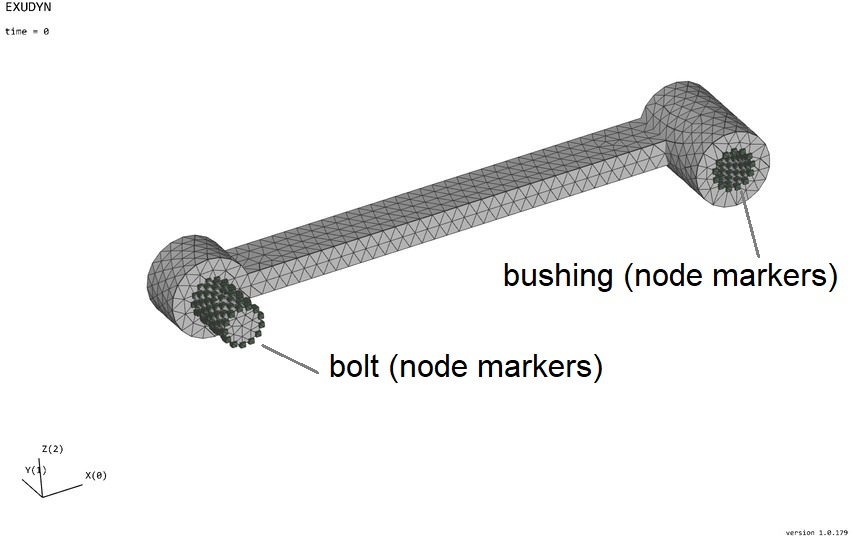
\includegraphics[width=10cm]{figures/modesHinge/HCBhingeMesh.jpg}
  \end{center}
  \caption{Test model and mesh for hinge created with Netgen (linear tetrahedral elements).}
	\label{fig_hingePartMesh}
\end{figure}
%++++++++++++++++++++++++
As an example, we consider a part denoted as 'hinge' in the following, see \fig{fig_hingePartMesh}. The test example can be found in \texttt{Examples/NGsolveCMStutorial.py} with lots of additional features.

After import of mass and stiffness matrix, eigenmodes and eigenfrequencies can be computed using \texttt{fem.ComputeEigenFrequencies(...)}, 
which computes the quantities \texttt{fem.modeBasis} and \texttt{fem.eigenValues}.
The eigenvalues in Hz can be retrieved also with the function \texttt{fem.GetEigenFrequenciesHz()}.
The function \texttt{fem.ComputeEigenFrequencies(...)} is available for dense and sparse matrices, and uses \texttt{scipy.linalg} to compute eigenvalues of the linear, undamped mechanical system
\be \label{theory:eigenmodes:EOM}
	\Mm \ddot \qv(t) + \Km \qv(t) = \fv(t) \eqDot
\ee
Here, the total number of coordinates of the system is $n$, 
thus having the vector of system coordinates $\qv \in \Rcal^n$, 
vector of applied forces $\fv \in \Rcal^n$, 
mass matrix $\Mm \in \Rcal^{n \times n}$ and stiffness matrix $\Km \in \Rcal^{n \times n}$. 
If we are interested in free vibrations of the system, without any boundary conditions or interconnections to other bodies, \eq{theory:eigenmodes:EOM} can be converted to a generalized eigenvalue problem. Using the approach 
$\qv(t) = \vv \mathrm{e}^{\mathrm{i} \omega t}$ in \eq{theory:eigenmodes:EOM}, and thus $\ddot \qv(t) = -\omega^2 \qv(t)$, we obtain
\be \label{theory:eigenmodes:harmonicEquation}
		\left[ \left(-\omega^2 \Mm + \Km \right) \vv \right] \mathrm{e}^{i\omega t} = \Null \eqDot
\ee
Assuming that \eq{theory:eigenmodes:harmonicEquation} is valid for all times, the {\bf generalized eigenvalue problem} follows that
\be \label{theory:eigenmodes:GEP}
	\left(-\omega^2 \Mm + \Km \right) \vv = \Null \eqComma
\ee
which can be rewritten as
\be \label{theory:eigenmodes:GEP2}
	\det \left(-\omega^2 \Mm + \Km \right) = 0 \eqComma
\ee
and which defines the eigenvalues $\omega_i^2$ of the linear system, where $i \in \{0, \ldots, n-1\}$. Note that in this case, the eigenvalues are the squared eigenfrequencies (in rad/s).
We can use eigenvalue algorithms to compute the eigenvalues $\omega_i^2$ and according eigenvectors $\vv_i$ from Python.
The function \texttt{fem.ComputeEigenmodes(...)} uses \texttt{eigh(...)} from \texttt{scipy.linalg} in the dense matrix mode, 
and in the sparse mode \texttt{eigsh(...)} from \texttt{scipy.sparse.linalg}, the latter being restricted to pure symmetric matrices.
Using special shift-inverted techniques in \texttt{eigsh(...)}, it performs much better than standard settings. However, you may tune your specific eigenvalue problem by modifying the solver procedure (just copy that function and adjust to your needs).
As an output, we obtain the smallest \texttt{nModes} eigenvectors (=eigenmodes)\footnote{Eigenvectors are the result of the eigenvalue algorithm, such as the QR algorithm. The mechanical interpretation of eigenvectors are eigenmodes, that can be visualized as shown in the figures of this section.} of the system.
Here, we will also use synonymously the terms `eigenmodes' and `normal modes', which result from an eigenvalue/eigenvector computation using certain (or even no) boundary conditions.
%++++++++++++++++++++++++
\begin{figure}[tbph]
  \begin{center}
  \includegraphics[width=4cm]{figures/modesHinge/freeFreeModeStress1}
  \includegraphics[width=4cm]{figures/modesHinge/freeFreeModeStress2}
  \includegraphics[width=4cm]{figures/modesHinge/freeFreeModeStress3}
  \includegraphics[width=4cm]{figures/modesHinge/freeFreeModeStress4}\\
  \includegraphics[width=4cm]{figures/modesHinge/freeFreeModeStress5}
  \includegraphics[width=4cm]{figures/modesHinge/freeFreeModeStress6}
  \includegraphics[width=4cm]{figures/modesHinge/freeFreeModeStress7}
  \includegraphics[width=4cm]{figures/modesHinge/freeFreeModeStress8}
  \end{center}
  \caption{Lowest 8 free-free modes for hinge finite element model, contour plot for $xx$-stress component.}
	\label{fig_hingePartFreeFreeModes}
\end{figure}
%++++++++++++++++++++++++

Clearly, if there are no supports included in the stiffness matrix, the resulting eigenmodes will contain 6 rigid body modes and we will also call this case for the computation of eigenmodes the `free-free' case, in analogy to a simply supported beam.
This rigid body modes, which are usually not needed (=unwanted) in the succeeding computation, can be excluded with an according option in \vspace{6pt}\\
\texttt{fem.ComputeEigenFrequencies(excludeRigidBodyModes = ...)}
\vspace{12pt}\\
For our test example, 8 eigenmodes are shown in \fig{fig_hingePartFreeFreeModes}, where the 6 rigid body modes have been excluded (so in total, 14 eigenvectors were computed).
%free free modes (coarse mesh, nNodes= 1216):
%freq(Hz)=[ 671.59137506  707.17488417 1298.50905491 1929.97563131 1971.76505866
%3141.47119938 3595.34508711 4317.51987533]
The 8 eigenfrequencies for the chosen coarse mesh with mesh size $h=0.01$ and 1216 nodes result as 
\be
  f_{0..7} = [ 671.59, 707.17, 1298.50, 1929.97, 1971.76, 3141.47, 3595.34, 4317.51] Hz
\ee
Note, that a computation with a finer mesh, using mesh size $h=0.002$ and 100224 nodes, leads to significantly different eigenfrequencies, starting with $f_0=371.50\,$Hz. This shows that quadratic finite elements would be more appropriate for this case.

After the computation of modes, it is always a good idea to visualize and/or animate these modes. We can do this, using the function \texttt{AnimateModes(...)} available in \texttt{exudyn.interactive}, which allows us to inspect and animate modes and to create animations for these modes, see the mentioned example.

Clearly, the free-free modes in \fig{fig_hingePartFreeFreeModes} are not well suited for the modeling of the deformations within the hinge, if the bolt and the bushing shall be fixed to ground or to another part. 
%TO BE DONE:
%We investigate this by adding a simple revolute joint to the bolt.
Therefore, we can use modes based on ideas of Hurty \cite{Hurty1965} and Craig-Bampton \cite{CraigBampton1968}, as shown in the following.


%+++++++++++++++++++++++++++++++++++++++++++++++++++++++++++++++++++++++++++++++++++++++++++++++++++++++++++++++++++++++
%+++++++++++++++++++++++++++++++++++++++++++++++++++++++++++++++++++++++++++++++++++++++++++++++++++++++++++++++++++++++
%+++++++++++++++++++++++++++++++++++++++++++++++++++++++++++++++++++++++++++++++++++++++++++++++++++++++++++++++++++++++
\mysubsubsection{Hurty-Craig-Bampton modes} \label{sec:hurty-craig-bampton-modes}
This section will describe the computation of static and eigen (normal) modes using FEMinterface.
The theory is based on Hurty \cite{Hurty1965} and Craig-Bampton \cite{CraigBampton1968}, but often only attributed to Craig-Bampton.
Furthermore, boundaries are also called interfaces\footnote{Here, and in the description of various Python functions, we will use boundary and interface often synonymously, as flexible bodies can be either connected to ground in the sense of a classical 'support-type' boundary condition, or they can represent the boundary of the flexible body as an interface to joints (via markers).}, as they either represent surface sections of our finite element model which are connected to the ground or they represent interfaces to joints and are connected to other bodies.

The computation of so-called static and normal modes follows a simple concept based on finite element mass and stiffness matrices.
The final goal of the computation of modes is to approximate the solution $\qv \in \Rcal^n$ 
by means of a reduction basis $\tPsi \in \Rcal^{n \times m}$ 
and a reduced set of coordinates $\pv \in \Rcal^m$, for which we assume $m \ll n$.

In order to include boundary/interface effects, we separate our nodes and the nodal coordinates into 
\bi
  \item[] a) boundary nodes $\qv_b \in \Rcal^{n_b}$ and
	\item[] b) internal or inner nodes $\qv_i \in \Rcal^{n_i}$.
\ei
We assume that internal nodes are not exposed to boundary/interface conditions or to forces.

Therefore, we may rewrite \eq{theory:eigenmodes:EOM} as follows
\be \label{eq_GuyanIrons}
	\mp{\Mm_{bb}}{\Mm_{bi}}{\Mm_{ib}}{\Mm_{ii}} \vp{\ddot{\qv}_b}{\ddot{\qv}_i} + \mp{\Km_{bb}}{\Km_{bi}}{\Km_{ib}}{\Km_{ii}} \vp{\qv_b}{\qv_i} =   \vp{\fv_b}{\Null}
\ee
or, equivalently,
\bea
	\Mm_{bb} \ddot{\qv}_b + \Mm_{bi} \ddot{\qv}_i +\Km_{bb}  {\qv}_b + \Km_{bi}  {\qv}_i  = {\fv}_b \label{eq_Guyan_bb}\\
	\Mm_{ib} \ddot{\qv}_b + \Mm_{ii} \ddot{\qv}_i +\Km_{ib}  {\qv}_b + \Km_{ii}  {\qv}_i  = \Null \eqDot \label{eq_Guyan_ii}
\eea
A pure static condensation follows from \eq{eq_Guyan_ii} with the assumption that inertia terms are neglected,
leading to the static result for internal nodes,
\be 
	{\qv}_{i,stat}=-\Km_{ii}^{-1} \Km_{ib} {\qv}_{b} \eqDot 
\ee
A pure static condensation, also denoted as Guyan-Irons method, keeps boundary coordinates but removes all internal modes, using the approximation
\be
	\label{eq_guans_red}
	\vp{\qv_b}{\qv_i} \approx \vp{\Im}{-\Km_{ii}^{-1} \Km_{ib}}  \qv_b = \tPsi^{GI} \qv_b \eqComma
\ee
which leads to no approximations ('exact') results for the static case, but poor performance in highly dynamic problems.

Significant improvement result from the Hurty-Craig-Bampton method, which adds eigenmodes of the internal coordinates (internal nodes).
We assume that $\tPsi_{ii}$ is the matrix of eigenvectors as a solution to the eigenvalue problem
\be \label{theory:eigenmodes:GEPii}
	\left(-\omega^2 \Mm_{ii} + \Km_{ii} \right) \vv = \Null \eqComma
\ee
Hereafter, we will only keep the lowest (or other appropriate) $m$ eigenmodes in a reduced eigenmode matrix,
\be
  \tPsi^{(red)}_{ii} = \left[\tPsi_{ii,0}, \ldots, \tPsi_{ii,m-1} \right]
\ee
Combining these `fixed-fixed' eigenvectors with the Guyan-Irons reduction \eqref{eq_guans_red}, we obtain the 
Hurty-Craig-Bampton modes as
\be
	\vp{\qv_b}{\qv_i} \approx \vp{\Im}{-\Km_{ii}^{-1} \Km_{ib}}  \qv_b  +  \vp{\Null}{\tPsi_{r,i}}  \pv_{r} \eqComma
\ee
or in matrix form
\be \label{theory:eigenmodes:HCB}
	\vp{\qv_b}{\qv_i} \approx \mp{\Im}{\Null}{-\Km_{ii}^{-1} \Km_{ib}}{\tPsi_{r,i}}   \vp{\qv_b}{\pv_r} = \tPsi^{HCB} \pv^{HCB} \eqDot
\ee
The disadvantage of \eq{theory:eigenmodes:HCB} is evident by the fact that there may be a large number of boundary/interface nodes, leading to a huge number of static modes (100s or 1000s) and thus making the model reduction inefficient. Therefore, we can switch to other interfaces, as described in the following.

\mysubsubsubsection{Definition of RBE2 / RBE3 interfaces}
A powerful extension, which is available in many finite element as well as flexible multibody codes, is the definition of special boundary/interface conditions, based on pure rigid body motion.
The so-called RBE2 boundaries are defined such that they are firmly connected to a rigid frame, thus the boundary or interface can only undergo rigid body motion.
The advantage of this procedure is that, in comparison to \eq{theory:eigenmodes:HCB}, the number of boundary/interface modes is given by 6 {\it rigid body} modes, which allow simple integration into standard joints of multibody systems, e.g., the \texttt{GenericJoint}.
The disadvantage is that such modes usually lead to artificial stiffening and stresses close to the boundary.

For so-called RBE3 boundaries, the kinematics is significantly different. The displacement of RBE3 boundaries is the (weighted) average displacement of all boundary nodes. The resulting forces at the RBE3 boundary are equally distributed, again using node-weighting.
The (linearized) rotation of RBE3 boundaries is computed as the weighted displacements of the boundaries and including the distance to the rotation axes. 
Forces due to torques at RBE3 boundaries are computed according to the weighting, again considering the distance to the rotation axes, see the according formulas later on. The computation of RBE3 boundaries widely follows the formulation of the \texttt{MarkerSuperElementRigid}, see \refSection{sec:item:MarkerSuperElementRigid}.

\mysubsubsubsection{Computation of Hurty-Craig-Bampton modes with RBE2 interfaces}
In the following section, we show the procedure for the computation of static modes for the RBE2 rigid-body interfaces.
Note that eigenmodes directly follow from matrices $\Mm_{ii}$ and $\Km_{ii}$ as described in \refSection{sec:hurty-craig-bampton-modes}.
The implementation is given in \texttt{fem.ComputeHurtyCraigBamptonModes(...)}, see \refSection{sec:FEM:FEMinterface:ComputeHurtyCraigBamptonModes}.

First, we use the index $j$ here as a node index, having the clear correspondence to the coordinate index $i$, that node $j$ has coordinates 
$[3\cdot j,\; 3\cdot j+1,\; 3\cdot j+2]$.
Furthermore, nodes are split into boundary and internal nodes, which then leads to according internal and boundary coordinates.
We shall note that this sorting is never done in the finite element model or matrices, but just some indexing (referencing) lists are generated and used throughout, using valuable features of \texttt{numpy.linalg} and \texttt{scipy.sparse}.

For a certain boundary node set $B=[j_0, \; j_1, \; j_2, \; ...] \in \Ncal^{n_b}$ with certain $n_b$ node indices $j_0, ...$, we define one boundary set. The following transformations need to be performed for every set of boundary node lists. We also assume that weighting of all boundary nodes is equal, which may not be appropriate in all cases.

If we assume that there may only occur rigid body translation and rotation for the whole boundary node set, which is according to the idea of so-called RBE2 boundary conditions, it follows that the translation of all boundary nodes is given by
\be
  %\Tm_t = \left[ \Im \; \Im \; \ldots \; \Im \right]\tp \in \Rcal^{3 n_b \times 3}
  \Tm_t = \vr{ \Im }{ \vdots}{ \Im} \in \Rcal^{3 n_b \times 3}
\ee
with $\Im \in \Rcal^{3\times 3}$ identity matrices. 
The nodal translation coordinates on boundary $B$ are denoted as $\qv_{B,t} \in \Rcal^3$. The translation of the boundary/interface is mapped to the boundary coordinates as follows (assuming only one boundary $B$),
\be
  \qv_{b,t} = \Tm_t \, \qv_{B,t}
\ee
The nodal rotation coordinates on boundary $B$ are denoted as $\qv_{B,r} \in \Rcal^3$. The rotation of the boundary/interface is mapped to the boundary coordinates as follows (assuming only one boundary $B$),
\be
  \qv_{b,r} = \Tm_r \, \qv_{B,r}
\ee
The computation of matrix $\Tm_r$ is more involved. It is based on nodal (reference) position vectors $\rv^{(0)}_j$, $j \in B$, 
the midpoint of all boundary nodes, 
\be
  \rv^{(m)} = \frac{1}{n_b} \sum_{j=0}^{n_b-1} \rv^{(0)}_j
\ee
and the position relative to the midpoint, denoted as 
\be
  \rv_j = \rv^{(0)}_j - \rv^{(m)} \eqDot
\ee
Note that the coordinate system refers to the system used in the underlying finite element mesh.
The transformation for rotation follows from 
\be
  %in old version, j should have been 0, 1, 2, ...
  %\Tm_r  = \left[ \widetilde \tOmega_x \rv_{j_0} \;\; \widetilde \tOmega_y \rv_{j_0} \;\; \widetilde \tOmega_z \rv_{j_0} \;\;
	                %\widetilde \tOmega_x \rv_{j_1} \;\; \widetilde \tOmega_y \rv_{j_1} \;\; \widetilde \tOmega_z \rv_{j_1}
									%\ldots \right]\tp \in \Rcal^{3 n_b \times 3}
  \Tm_r = \vr{ \tilde \rv_0 }{ \vdots}{ \tilde \rv_{n_b-1}} \in \Rcal^{3 n_b \times 3} \eqDot
\ee
%with the special tensors, representing rotation about (x,y,z)-axes,
%\be
  %\widetilde\tOmega_x = \mr{0}{0}{0} {0}{0}{-1} {0}{1}{0}, \quad
  %\widetilde\tOmega_y = \mr{0}{0}{1} {0}{0}{0} {-1}{0}{0}, \quad
  %\widetilde\tOmega_z = \mr{0}{-1}{0} {1}{0}{0} {0}{0}{0} \eqDot
%\ee
%
The total nodal coordinates at the boundary, representing translations and rotations, follow as
\be
  \qv_{B} = \vp{\qv_{B,t}}{\qv_{B,r}} \eqComma
\ee
and the transformation matrix for the translation and rotation simply reads
\be
  \Tm = [\Tm_t \;\; \Tm_r] \in \Rcal^{3n_b \times 6} \eqComma
\ee
which provides the total mapping of boundary rigid body motion
\be
  \qv_{b} = \Tm \, \qv_{B} \eqComma
\ee 
which is the sum of translation and rotation.

As an example, having the boundary nodes sorted for two boundary node set $B_0$ and $B_1$, we obtain the following transformation for the Hurty-Craig-Bampton method with only 6 modes per boundary node set,
\be \label{theory:eigenmodes:HCBRBE2}
	%\vp{\qv_b}{\qv_i} \approx \mp{ \Im \mp{\Tm_0}{}{}{\Tm_1}}{\Null}{-\Km_{ii}^{-1} \Km_{ib}\vp{\Tm_0}{\Tm_1}}{\tPsi_{r,i}}   
	%\vr{\qv_{B_0}}{\qv_{B_1}}{\pv_r} \eqDot
	\vp{\qv_b}{\qv_i} \approx \mr{ \Tm_0}{\Null}{\Null} {\Null}{\Tm_1}{\Null} 
	                          {-\Km_{ii}^{-1} \Km_{ib}\vp{\Tm_0}{\Null} }{-\Km_{ii}^{-1} \Km_{ib}\vp{\Null}{\Tm_1} }{\tPsi_{r,i}}   
	\vr{\qv_{B_0}}{\qv_{B_1}}{\pv_r} \eqDot
\ee
with the new boundary node vector $\qv_b = [\qv_{B_0}\tp \;\; \qv_{B_1}\tp]\tp$.
%\newcommand{\mr}[9]{\left[\!\! \begin{array}{ccc} #1 & #2 & #3 \vspace{0.1cm}\\ #4 & #5 & #6 \vspace{0.1cm}\\ #7 & #8 & #9  \end{array} \!\!\right]}

\noindent {\bf Notes}:
\bi
  \item The inverse $\Km_{ii}^{-1} $ is not computed, but this matrix is LU-factorized using sparse techniques.
	\item The factorization only needs to be applied to six vectors for every relevant boundary node set.
	\item One set of boundary nodes can be omitted from the final static modes in \eq{theory:eigenmodes:HCBRBE2}, because keeping all boundary modes, would introduce six rigid body motions to our mode basis, what is usually not wanted nor needed.
\ei

Using again the examples given in \fig{fig_hingePartMesh}, we now obtain a set of modified modes using the function \texttt{fem.ComputeHurtyCraigBamptonModes(...)}.
\fig{fig_hingePartStaticModesA} shows the first 6 rigid body modes. Note that these modes are automatically removed in the function \texttt{fem.ComputeHurtyCraigBamptonModes(...)} with default settings.
\fig{fig_hingePartStaticModesB} shows the second set of 6 rigid body modes. 
Finally, 8 eigenmodes have been computed for the fixed-fixed case (where all boundary/interfaces nodes are fixed),
see \fig{fig_hingePartFixedFixedModes}. 
The eigenfrequencies for this case now are significantly higher than in the free-free case, reading
\be
  f_{0..7} = [1277.35, 1469.86, 3336.91, 3584.28, ...]
\ee
%Hurty-Craig-Bampton modes (coarse mesh, nNodes= 1216):
 %freq(Hz)=[1277.35052832 1469.86514681 3336.91168906 3584.28464361 5079.65220372
 %6035.58805197 6049.99829894 6568.47108075]
%++++++++++++++++++++++++
\begin{figure}[tbph]
  \begin{center}
  \includegraphics[width=5cm]{figures/modesHinge/HCBmodesHingeStaticAx}
  \includegraphics[width=5cm]{figures/modesHinge/HCBmodesHingeStaticAy}
  \includegraphics[width=5cm]{figures/modesHinge/HCBmodesHingeStaticAz}\\
  \includegraphics[width=5cm]{figures/modesHinge/HCBmodesHingeStaticArotX}
  \includegraphics[width=5cm]{figures/modesHinge/HCBmodesHingeStaticArotY}
  \includegraphics[width=5cm]{figures/modesHinge/HCBmodesHingeStaticArotZ}
  \end{center}
  \caption{Static modes for bolt rigid body interface, using Hurty-Craig-Bampton method; top three images show (x,y,z)-translation modes, bottom three images show (x,y,z)-rotation modes; contour color represents norm of displacements.}
	\label{fig_hingePartStaticModesA}
\end{figure}
%++++++++++++++++++++++++

%++++++++++++++++++++++++
\begin{figure}[tbph]
  \begin{center}
  \includegraphics[width=5cm]{figures/modesHinge/HCBmodesHingeStaticBx}
  \includegraphics[width=5cm]{figures/modesHinge/HCBmodesHingeStaticBy}
  \includegraphics[width=5cm]{figures/modesHinge/HCBmodesHingeStaticBz}\\
  \includegraphics[width=5cm]{figures/modesHinge/HCBmodesHingeStaticBrotX}
  \includegraphics[width=5cm]{figures/modesHinge/HCBmodesHingeStaticBrotY}
  \includegraphics[width=5cm]{figures/modesHinge/HCBmodesHingeStaticBrotZ}
  \end{center}
  \caption{Static modes for bushing rigid body interface, using Hurty-Craig-Bampton method; top three images show (x,y,z)-translation modes, bottom three images show (x,y,z)-rotation modes; contour color represents norm of displacements.}
	\label{fig_hingePartStaticModesB}
\end{figure}
%++++++++++++++++++++++++

%++++++++++++++++++++++++
\begin{figure}[tbph]
  \begin{center}
  \includegraphics[width=4cm]{figures/modesHinge/HCBmodesHingeEigenmode0}
  \includegraphics[width=4cm]{figures/modesHinge/HCBmodesHingeEigenmode1}
  \includegraphics[width=4cm]{figures/modesHinge/HCBmodesHingeEigenmode2}
  \includegraphics[width=4cm]{figures/modesHinge/HCBmodesHingeEigenmode3}\\
  \includegraphics[width=4cm]{figures/modesHinge/HCBmodesHingeEigenmode4}
  \includegraphics[width=4cm]{figures/modesHinge/HCBmodesHingeEigenmode5}
  \includegraphics[width=4cm]{figures/modesHinge/HCBmodesHingeEigenmode6}
  \includegraphics[width=4cm]{figures/modesHinge/HCBmodesHingeEigenmode7}
  \end{center}
  \caption{Eigenmodes for fixed-fixed case, resulting from Hurty-Craig-Bampton method; contour color represents norm of displacements.}
	\label{fig_hingePartFixedFixedModes}
\end{figure}
%++++++++++++++++++++++++


%+++++++++++++++++++++++++++++++++++++++++++++++++++++++++++++++++++++++++++++++++++++++
%+++++++++++++++++++++++++++++++++++++++++++++++++++++++++++++++++++++++++++++++++++++++
%synchronize this section with the paper!
%\mysubsubsubsection{Computation of Hurty-Craig-Bampton modes with RBE3 interfaces}
%In the following section, we show the procedure for the computation of static and eigenmodes for the RBE3 rigid-body interfaces.
%The implementation is given in \texttt{fem.ComputeHurtyCraigBamptonModes(...)}, see \refSection{sec:FEM:FEMinterface:ComputeHurtyCraigBamptonModes}.
%
%It shall be noted that there are slightly different versions of RBE3 modes, as there are several possibilities to define average displacements and rotations,
%and there are several ways to define the eigen-problem for eigenmodes.
%Here, we chose the following way to compute eigenmodes:
%\bi
  %\item at every boundary, which may not contain overlapping nodes with other boundaries, the weighted average displacement and the weighted average rotation is fixed by imposing 6 constraints per boundary;
  %\item for the computation of static modes, a single DOF at the rigid boundaries is prescribed with an average unit displacement or unit rotation.
  %\item for the computation of eigenmodes, all weighted displacements/rotations are fixed and eigenmodes are computed for lowest eigenfrequencies.
%\ei
%%
%The stiffness matrix, sorted for boundary and internal nodal coordinates reads, compare \eq{eq_GuyanIrons},
%\be
  %\Km = \mp{\Km_{bb}}{\Km_{bi}}{\Km_{ib}}{\Km_{ii}}
%\ee
%
%\noindent
%For every boundary $B \in [B0, B1, \ldots ]$ of $n_B$ boundaries, we defined linear constraints, using the same boundary node definitions as for RBE2 boundaries.
%The three linear constraints for average displacements are given for boundary nodes $j$ with displacement vectors $\qv_{b,j}$ and nodal weights per boundary $w_{B,j}$\footnote{note that the sum of all weights follows as $\sum_j w_{B,j}=1$.}, 
%\be
  %\cv_{b,t}(\qv_b) = \Cm_{b,t} \qv_b = \sum_{j=0}^{n_B-1} w_{B,j} \qv_{B,j} = \uv_B
%\ee
%which implicitly defines $\Cm_{b,t} \in \Rcal^{3 n_b \times 3}$, while $\Cm_{i,t} = \Null \in \Rcal^{3 n_i \times 3}$.
%The prescribed displacement $\uv_B$ is zero, except that this boundary mode is currently computed.
%
%For rotations, the nodal (reference) position vectors $\rv^{(0)}_j$, $j \in B$ and
%the midpoint of all boundary nodes, 
%\be
  %\rv^{(m)} = \frac{1}{n_b} \sum_{j=0}^{n_B-1} w_{B,j} \rv^{(0)}_j \eqComma
%\ee
%are again used to define positions relative to the midpoint $\rv^{(m)}$, 
%\be
  %\rv_j = \rv^{(0)}_j - \rv^{(m)} \eqDot
%\ee
%Note that the coordinate system refers to the system used in the underlying finite element mesh.
%Similar as in the \texttt{MarkerSuperElementRigid}, see \refSection{sec:item:MarkerSuperElementRigid}, 
%we define a total weighting for all nodal reference positions relative to the boundary's midpoint as
%\be
    %\Wm = -\sum_j  w_{B,j} \tilde \rv_j \tilde \rv_j \eqComma
%\ee
%which follows from the analogy of an inertia tensor with mass distributed equally at the boundary.
%
%The three linear constraints for average rotations follow as
%\be
  %\cv_{b,r}(\qv_b) = \Cm_{b,r} \qv_b = \sum_{j=0}^{n_B-1} w_{B,j} \tilde \rv_{B,j} \qv_{B,j}  = \ttheta_B
%\ee
%which implicitly defines $\Cm_{b,r} \in \Rcal^{3 n_b \times 3}$.
%Here, $\ttheta_B$ is a weighting matrix similar to the \texttt{MarkerSuperElementRigid},
%\be
  %\ttheta_B = \sum_{j=0}^{n_B-1} -w_{B,j} \tilde \rv_{B,j} \tilde \rv_{B,j}
%\ee
%Similarly as for translations, the prescribed rotation $\ttheta_B$ is zero, except that this boundary mode is currently computed.
%Finally, we combine translation and rotation part as 
%\be
  %\Cm_{b} = \vp{\Cm_{b,t}}{\Cm_{b,r}} \eqComma
%\ee
%and set $\Cm_{i} = \Null \in \Rcal^{3 n_i \times 6}$.
%In order to compute boundary modes, the linear system of equations reads
%\be \label{eq:theory:HCB:RBE3linearEq}
  %\mr{\Km_{bb}}{\Km_{bi}}{\Cm_{b}\tp} {\Km_{ib}}{\Km_{ii}}{\Cm_{i}\tp} {\Cm_{b}}{\Cm_{i}}{\Null} \vr{\qv_b}{\qv_i}{\tlambda} = \vr{\Null}{\Null}{\tdelta} \eqDot
%\ee
%Here, $\tlambda$ represents Lagrange multipliers which represent the boundary forces and torques at the according boundaries due to unit displacements or rotations, given by the vector $\tdelta$.
%In order to compute the $k^\mathrm{th}$ boundary mode as $\vp{\qv_b^k}{\qv_i^k}$, we set the $k^\mathrm{th}$ component of $\tdelta$ to
%\be
  %\tdelta_k = 1 \eqComma
%\ee
%while all other components of $\tdelta$ are $0$ and solve \eq{eq:theory:HCB:RBE3linearEq}. This way allows to compute all static modes using a single factorization in \eq{eq:theory:HCB:RBE3linearEq} to compute all modes for all boundaries.
%
%The computation of eigenmodes require to apply all constraints to the stiffness and mass matrices, which is done by means of projection of the linear equations of motion into the null space of the constraints.
%We compute the singular value decomposition for every constraint matrix $\Cm_{b}$,
%\be
  %[\Um, \sv, \Vm] = \mathrm{SVD}(\Cm_{b}), \eqComma
%\ee
%where $\Um$ is a unitary matrix with left singular vectors as columns, $\sv$ stores singular values in the diagonal, and $\Vm$ is a 
%unitary matrix with right singular vectors as rows.
%The null space of the constraint matrix $\Cm_{b}$ is spanned by $\Vm_N \in \Rcal^{(3 n_b-6) \times 3 n_b}$, which results from $\Vm$ when removing the first 6 rows. 
%Combining the null space matrix with a unit matrix for the internal nodes, $\Im_{ii} \in \Rcal^{n_i \times n_i}$,
%the projection matrix results as
%\be
  %\Vm_P = \mp{\Vm_N}{}{}{\Im_{ii}}
%\ee
%Using the projected stiffness and mass matrices,
%\be
	%\Mm_P = \Vm_P \mp{\Mm_{bb}}{\Mm_{bi}}{\Mm_{ib}}{\Mm_{ii}} \Vm_P\tp \quad \mathrm{and} \quad
  %\Km_P = \Vm_P \mp{\Km_{bb}}{\Km_{bi}}{\Km_{ib}}{\Km_{ii}} \Vm_P\tp 
%\eqComma
%\ee
%the eigenvalue problem for the constrained system of \eq{eq:theory:HCB:RBE3linearEq} is given by
%\be \label{eq:theory:HCB:RBE3eigen}
	%\Mm_P \ddot{\qv}_P + \Km_P \qv_P = \Null \eqDot
%\ee
%The eigen analysis of \eq{eq:theory:HCB:RBE3eigen} results in the eigenvector matrix $\tPsi_P \in \Rcal^{(n-6) \times m}$, containing a set of $m$ eigenvectors.
%The final eigenvectors $\tPsi \in \Rcal^{n \times m}$ are computed by means of projection onto the original boundary nodes, using
%\be
  %\tPsi = \Vm_P\tp \tPsi_P \eqDot
%\ee
%Note that for efficiency reasons operations such as in \eq{eq:theory:HCB:RBE3eigen} are only performed for boundary nodes, but not for internal nodes.
%Furthermore, sparse matrices are used whenever matrices are large and not fully populated.
%


%+++++++++++++++++++++++++++++++++++++++++++++++++++++++++++++++++++++++++++++++++++++++
\mysubsubsection{Interfaces and boundaries}
\label{sec:theory:CMS:interfaces}
Being able to model a sole flexible body is not sufficient for the modeling of industrial problems.
An important part of component mode synthesis is the appropriate definition of boundaries or interfaces.
The term interface is widely used and may be more appropriate when connecting two bodies via such interfaces.
However, in some cases the flexible body may be fixed to ground via such a boundary. In order to distinguish boundary/interface (b) and internal nodes (i), boundary seems to be appropriate and boundary/interface will be used synonymously in the context of flexible bodies.

An boundary/interface is represented by a certain surface area of a body, usually defined by surface elements and underlying nodes.
For simplicity, it may just be defined by means of a node set.
This is sufficient, in order for most of the previously described algorithms to work.
If node sets are not imported from the underlying finite element codes, practical functions exist for the definition of
node sets from geometrical operations, specifically\footnote{Note that these functions perform a linear search in the whole mesh, which is computationally inefficient if it is called many times.}:
\bi
  \item \texttt{GetNodeAtPoint}: returns node number of a single node (if found) at given spatial position, with certain tolerance
  \item \texttt{GetNodesInPlane}: returns all nodes lying on a defined plane with certain tolerance
  \item \texttt{GetNodesInCube}: returns all nodes lying in a axis-parallel cube
  \item \texttt{GetNodesOnLine}: returns all nodes lying on a line defined by two points, with certain tolerance
  \item \texttt{GetNodesOnCylinder}: returns all nodes lying on a cylinder defined by two points and radius, with certain tolerance
  \item \texttt{GetNodesOnCircle}: returns all nodes lying on a circle defined by point, normal and radius, with certain tolerance
\ei
In order to compute according weighting factors, surface elements need to exist, either importing them the finite element code, or by using the \texttt{FEMinterface} member \texttt{surface}.
The surface of tetrahedral or hexahedral meshes, which follow a standard node numbering, can be computed using
the \texttt{FEMinterface} function \texttt{VolumeToSurfaceElements}.


%+++++++++++++++++++++++++++++++++++++++++++++++++++++++++++++++++++++++++++++++++++++++
\mysubsubsection{Node weighting}
\label{sec:theory:CMS:nodeWeighting}
%
As mentioned in the literature \cite{HeirmanDesmet2010}, there are certain advantages to use regular meshes on boundaries/interfaces.
However, industrial relevant geometries often cannot be meshed by regular hexahedral meshes which leads to unstructured tetrahedral elements with (nearly) arbitrary triangular surfaces.
While being a more general approach, an according nodal weighting is inevitable for unstructured surface meshes.
As a drawback, accurate nodal weighting for application of forces or for computation of average displacements or rotations requires the information of underlying finite element interpolation functions, which are avoided in the present approach.
A simplified, first order accurate functionality is provided by \texttt{GetNodeWeightsFromSurfaceAreas}, which reconstructs nodal weights for a set of node numbers from a given triangulated surface in \texttt{FEMinterface}.
After identification of surface triangles and computation of according triangle areas, the weight $w_i$ of every node $i$ is built upon the according area of all connected triangles $j$,
\be
  w_i = \frac{1}{3 A_B} \sum_{j} A_j  \eqComma \quad \mathrm{and} \quad \sum_i w_i = 1
\ee
using the total area $A_B$ of the boundary. 
This weighting leads to nearly constant strain distribution along the cross section of a fixed bar with equally distributed axial forces.

%+++++++++++++++++++++++++++++++++++++++++++++++++++++++++++++++++++++++++++++++++++++++
\mysubsubsection{Reference conditions}
\label{sec:theory:CMS:referenceConditions}
%
Currently, there is no specific functionality to define reference conditions for \ac{FFRF} objects in \codeName\ .
In the \texttt{ObjectFFRF}, a \texttt{ObjectConnectorCoordinateVector} needs to be used to define constraints of a so-called Tisserand frame.

In the \texttt{ObjectFFRFreducedOrder}, there are in general two approaches:
\bi
  \item The computed modes do not include rigid body motions, by using the appropriate flag\\ \texttt{excludeRigidBodyModes = True}\\ for most of such functions; in this case, the reference conditions are defined such that the reference node positions of the mesh are rigidly attached to the reference frame. In case of Hurty-Craig-Bampton modes, one boundary set (the first one) is attached to the reference frame.
  \item Alternatively, \texttt{excludeRigidBodyModes} can be set False, or arbitrary modes can be imported from elsewhere.
    In this case, rigid body motion must be excluded by appropriate constraints, e.g., a \texttt{ObjectConnectorCoordinateVector} applied to the \texttt{NodeGenericODE2} of \texttt{ObjectFFRFreducedOrder}. This task is completely left to the user.
\ei
It should be noted that regarding efficiency or highest accuracy, better reference conditions may exists, which are not fully supported in the current code and may only be applied with user functions.





















\clearpage
%+++++++++++++++++++++++++++++++++++++++++++++++++++++++++++++++++
\mysubsection{Modeling of Contact in \codeName }
\label{secContactTheory}
% 
The \texttt{GeneralContact} module, see \refSection{sec:GeneralContact},  which is 
\bi
  \item[] {\bf still under developement, consider with care!}
\ei
provides a simple, efficient and versatile interface to a general contact module. The movivation for this module is based on the need for simple contact modeling in robotics, but also for the efficient modeling of beam-cylinder or beam-beam contact, as well as contact between deformable meshes (not yet available).

Note that there are currently only simplistic contact models, such as linear contact and simple damping, which are not representing realistic Hertzian contact (which will be implemented in near future). Furthermore, read the notes in \texttt{GeneralContact} carefully, how stiffness and damping is realized -- e.g., stiffness may be a serial spring against the other object, while damping is implemented as parallel damper.

%++++++++++++++++++++++++++++++++++++++++++++++++++++++++++++++++++++++++
\begin{figure}[hb]
  \centering
	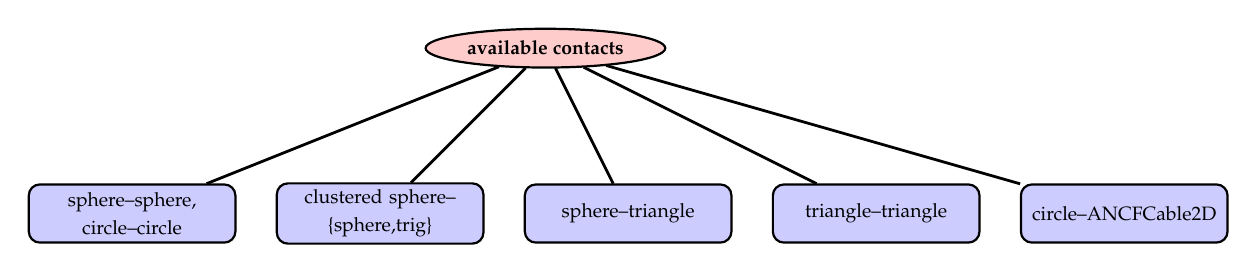
\begin{tikzpicture}[node distance = 2cm, auto, thick,scale=0.7, every node/.style={scale=0.7}]
			% Place nodes
			\node [cloud] (availableContacts) {{\bf available contacts}};
			\node [wideblock, below of=availableContacts, node distance=3cm, xshift = -7.5cm] (sphericalContact) {sphere--sphere, circle--circle};
			\node [wideblock, right of=sphericalContact, node distance=4.5cm] (clusteredSphericalContact) {clustered sphere--\{sphere,trig\}};
			\node [wideblock, right of=clusteredSphericalContact, node distance=4.5cm] (sphereTrigContact) {sphere--triangle};
			\node [wideblock, right of=sphereTrigContact, node distance=4.5cm] (trigTrigContact) {triangle--triangle};
			\node [wideblock, right of=trigTrigContact, node distance=4.5cm] (circleCableContact) {circle--ANCFCable2D};
			\path [line] (availableContacts) -- (sphericalContact);
			\path [line] (availableContacts) -- (clusteredSphericalContact);
			\path [line] (availableContacts) -- (sphereTrigContact);
			\path [line] (availableContacts) -- (trigTrigContact);
			\path [line] (availableContacts) -- (circleCableContact);
	\end{tikzpicture}
  \caption{Contact: possible coupling of geometrical objects in \codeName\ }
	\label{fig_available_contact}
\end{figure}
%++++++++++++++++++++++++++++++++++++++++++++++++++++++++++++++++++++++++
%

\noindent \fig{fig_available_contact} shows the implemented / possible coupling of contact objects:
\bi
  \item[1)] simulate spherical particles; in 2D, spheres are represented as circles
  \item[2)] simulate clustered spherical [circular] particles which consist of rigid bodies made of a cluster of spheres; several contact spheres are attached to one rigid body by using rigid body markers; in 2D, spheres are represented as circles
  \item[3)] simulate the contact of spheres with triangular meshes, e.g., in order to provide some limitations of the range of motion for your objects
  \item[4)] simulate the contact between arbitrarily shaped rigid bodies
  \item[5)] simulate the contact between rolls (spheres) and ANCF cable elements; to enable cable-cable contact, spheres must be attached and distributed along the cable elements
\ei
In all use cases, explicit integrators are much faster and they are recommended, as long as your problem allows to do so.
%
\mysubsubsection{Contact of meshed rigid bodies}
Case 4) is more involved and needs further explanations (which more or less also applies to case 4). The geometry is approximated by a mesh consisting of flat triangles, which are attached to a rigid body (marker). The triangles obtain a contact stiffness against spheres. There are special cases, depending if the sphere gets in contact with the triangle plane or with the triangle edge. Having contact with edges, usually involves several triangles at the same time (specifically at vertices), which leads to higher contact stiffness as compared to a planar contact. Nevertheless, for flat planes, contact computation takes care, that contact stiffness is constant in the whole plane, independently of the number of involved triangles.
In order to realize contact between meshed rigid bodies, both body-attached meshes are added via the \texttt{GeneralContact} function 
\bi
  \item \texttt{AddTrianglesRigidBodyBased(...)}
\ei
In addition, all mesh vertices are added as spheres with markers using 
\bi
  \item \texttt{AddSphereWithMarker(...)}
\ei
However, as we need a certain finite radius of the spheres, the mesh must be shrinked for this purpuse (and it needs to have according thickness). Shrinking of the (consistent) triangular mesh can be done by the utility function 
\bi
  \item \texttt{ ShrinkMeshNormalToSurface(...)};
  \item in order to reduce artifacts at object edges, it is recommended to refine the mesh, using the utility function \texttt{RefineMesh(...)}
\ei
According examples can be found in test models, but there will be a more convenient function for contact of meshes attached to rigid bodies in the future.

All contacts can be created in a \texttt{GeneralContact} object -- which is not a regular object in mbs -- created by
\bi
  \item \texttt{gContact = mbs.AddGeneralContact()}
\ei
Note that one can create several, independent contact objects.
Hereafter, spheres, triangles, ... are added with appropriate functions, see \refSection{sec:GeneralContact}.
Note that triangles need to be correctly numbered (see correct normals in \fig{fig:triangleNormals}), %in GraphicsData section!
which defines inside/outside of a triangluar mesh.

\mysubsubsection{Regularized friction}
Within a regularized friction law, similar to a well known law attributed to Haff-Werner, the friction force $\fv_f$ is computed from static (dry) friction coefficient $\mu_s$ and the friction regularization velocity\footnote{global regularization coefficient stored in \texttt{GeneralContact.frictionProportionalZone}} $v_{\mu,reg}$
\bea \label{eq_GeneralContactRegularizedFriction}
  v_t &=& |\LU{0}{\vv_t}|, \nonumber \\
  \fv_f &=& 
  \begin{cases}
    \frac{\mu_s \cdot |f_c|}{v_{\mu,reg}}\LU{0}{\vv_t}, \quad \mathrm{if} \quad v_t < v_{\mu,reg} \\
%    
    \mu_s \cdot |f_c| \frac{\LU{0}{\vv_t}}{v_t} , \quad \mathrm{else} 
  \end{cases}
\eea
%
{\bf Note} that the following equations represent the computed contact relations in high detail, but minor cases and flags, such as the \texttt{intraSpheresContact} are not described here, but must be carefully considered in the description of \texttt{GeneralContact}, see \refSection{sec:GeneralContact}.

%++++++++++++++++++++++++++++++++++++++++++++++++++++++++++++++++++++++++
%++++++++++++++++++++++++++++++++++++++++++++++++++++++++++++++++++++++++
%
\mysubsubsection{Sphere-sphere contact: Equations}
\label{secContactSphereSphere}
%
The equations for sphere-sphere contact in contact normal direction are very similar to the \texttt{ObjectConnectorSpringDamper}, see \refSection{sec:item:ObjectConnectorSpringDamper}.
%
Every sphere is attached to a position-based marker \footnote{which can be attached itself to position nodes, rigid body nodes, point masses, rigid bodies as well as flexible bodies. NOTE, that in case of implicit integration, flexible bodies are not fully implemented!}.
%
In C++, the sphere attached to marker 0 is denoted as \texttt{sphereI} and 
the sphere attached to marker 1 is denoted as \texttt{sphereJ}.
%
Input parameters for this contact model are
\startTable{intermediate variables}{symbol}{description}
\rowTable{sphere $i$ radius}{$r_i$}{radius of sphere $i$, attached to marker 0}
\rowTable{sphere $j$ radius}{$r_j$}{radius of sphere $j$, attached to marker 1}
\rowTable{sphere $i$ contact stiffness}{$k_i$}{N/m}
\rowTable{sphere $j$ contact stiffness}{$k_j$}{N/m}
\rowTable{sphere $i$ contact damping}{$d_i$}{N/m}
\rowTable{sphere $j$ contact damping}{$d_j$}{N/m}
\rowTable{friction pairing coefficient}{$\mu_{ij}$}{the friction coefficient stored in the the friction pairings matrix, resulting from the friction indices of spheres $i$ and $j$}
\finishTable

Marker positions and velocities are given by the relations:
\startTable{intermediate variables}{symbol}{description}
\rowTable{sphere $i$ position}{$\LU{0}{\pv}_{m0}$}{current global position which is provided by marker m0}
\rowTable{sphere $j$ position}{$\LU{0}{\pv}_{m1}$}{current global position which is provided by marker m1}
\rowTable{marker m0 position Jacobian}{$\LU{0}{\Jm_{pos,m0}}$}{with interpretation as variation of the position $\delta \LU{0}{\pv}_{m0} = \LU{0}{\Jm_{pos,m0}} \delta \qv_{m0}$; assuming that $\qv_{m0}$ represents the generalized coordinates of marker $m0$}
\rowTable{marker m1 position Jacobian}{$\LU{0}{\Jm_{pos,m1}}$}{with interpretation as variation of the position $\delta \LU{0}{\pv}_{m1} = \LU{0}{\Jm_{pos,m1}} \delta \qv_{m1}$; assuming that $\qv_{m0}$ represents the generalized coordinates of marker $m0$}
\rowTable{sphere $i$ velocity}{$\LU{0}{\vv}_{i}$}{current global velocity which is provided by marker m0}
\rowTable{sphere $j$ velocity}{$\LU{0}{\vv}_{j}$}{}
\rowTable{relative position}{$\LU{0}{\nv}$}{$\LU{0}{\pv}_{j} - \LU{0}{\pv}_{i}$}
%\rowTable{relative velocity$^*$}{$\Delta\! \LU{0}{\vv}$}{$\LU{0}{\vv}_{m1} - \LU{0}{\vv}_{m0}$}
\rowTable{Distance$^*$}{$L = |\LU{0}{\nv}|$}{}
\rowTable{unit vector$^*$}{$\LU{0}{\nv_0} = \frac{1}{L} \LU{0}{\nv}$}{vector in contact normal direction}
\rowTable{gap$^*$}{$g = L - (r_i + r_j)$}{}
\rowTable{penetration$^*$}{$p  = -g = r_i + r_j - L$}{}
\finishTable

In case of rigid bodies and non-zero friction, we also compute angular velocities and orientation,
\startTable{intermediate variables: rigid bodies and friction}{symbol}{description}
\rowTable{sphere $i$ angular velocity}{$\LU{m0}{\tomega}_{i}$}{current local angular velocity provided by marker $m0$}
\rowTable{marker $m0$ orientation}{$\LU{0,m0}{\Am}$}{transformation from marker m0 (body-fixed) to global coordinates}
\rowTable{sphere $j$ angular velocity}{$\LU{m1}{\tomega}_{j}$}{current local angular velocity provided by marker $m1$}
\rowTable{marker $m1$ orientation}{$\LU{0,m1}{\Am}$}{transformation from marker m0 (body-fixed) to global coordinates}
\rowTable{marker $m0$ rotation Jacobian}{$\LU{0}{\Jm_{rot,m0}}$}{with interpretation as derivative of the global angular velocity $\LU{0}{\tomega}_{m0} = \LU{0}{\Jm_{rot,m0}} \dot \qv_{m0}$; assuming that $\dot \qv_{m0}$ represents the generalized velocities of marker $m0$}
\rowTable{marker $m1$ rotation Jacobian}{$\LU{0}{\Jm_{rot,m1}}$}{with interpretation as derivative of the global angular velocity $\LU{0}{\tomega}_{m1} = \LU{0}{\Jm_{rot,m1}} \dot \qv_{m1}$; assuming that $\dot \qv_{m1}$ represents the generalized velocities of marker $m1$}
\finishTable


%
\newcommand{\diffANCF}[1]{\frac{\partial #1}{\partial \qv_{ANCF}}}
\newcommand{\diffANCFt}[1]{\frac{\partial #1}{\partial \dot \qv_{ANCF}}}
\newcommand{\diffANCFmI}[1]{\frac{\partial #1}{\partial \qv_{ANCF,m1}}}
\newcommand{\diffANCFmIt}[1]{\frac{\partial #1}{\partial \dot \qv_{ANCF,m1}}}
\newcommand{\diffmI}[1]{\frac{\partial #1}{\partial \qv_{m1}}}
\newcommand{\diffmIt}[1]{\frac{\partial #1}{\partial \dot \qv_{m1}}}
\newcommand{\diffmO}[1]{\frac{\partial #1}{\partial \qv_{m0}}}
\newcommand{\diffmOt}[1]{\frac{\partial #1}{\partial \dot \qv_{m0}}}
\newcommand{\diffmOI}[1]{\frac{\partial #1}{\partial \qv_{m0,m1}}}
\newcommand{\diffmOIt}[1]{\frac{\partial #1}{\partial \dot \qv_{m0,m1}}}
%
%
\noindent Contact between spheres with global index $g_i$ and another sphere with global index $g_j$ is active, if
\bi
  \item Bounding box of sphere $g_j$ intersects with a box in the searchtree which also intersects with bounding box of sphere $g_i$ AND
  \item if Bounding box of sphere $g_j$ intersects with bounding box of sphere $g_i$ AND
  \item if the condition $L^2 < \left(r_i + r_j\right)^2$ holds OR
  if $g_j$ belongs to the active set of $g_i$ (computed in PostNewtonStep).
\ei
Note that quantities $^*$ are only computed if contact is active.

\mysubsubsubsection{Contact relations for sphere $g_i$ (marker $m0$) and sphere $g_j$ (marker $m1$)}
\noindent If contact is active, we compute the global position of the contact point\footnote{considering also penetration, a more consistent contact point would be $\LU{0}{\pv_{c}^*} = \LU{0}{\pv_{m0}} + (r_i - \frac{p}{2}) \cdot \nv_0$, subtracting the half penetration.}, see \fig{fig_GeneralContactSpheres}
\be
  \LU{0}{\pv_{c}} = \LU{0}{\pv_{m0}} + r_i \cdot \nv_0 \eqComma
\ee
%++++++++++++++++++++++++
\begin{figure}[tbp]
  \begin{center}
  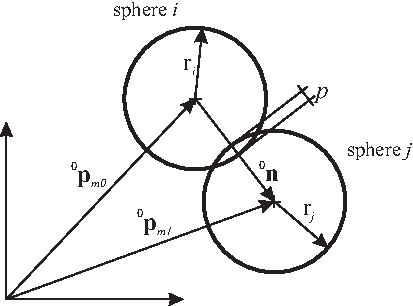
\includegraphics[width=8cm]{figures/generalContactSpheres}
  \end{center}
  \caption{Geometrical relations for contact of two spheres $i$ and $j$ with according markers $m0$ and $m1$.}
	\label{fig_GeneralContactSpheres}
\end{figure}
%++++++++++++++++++++++++
the velocities of the spheres at the contact point\footnote{In case of no friction, the angular velocities are not included in these relations},
\bea
  \LU{0}{\vv_{c,i}} &=& \LU{0}{\vv_i} + \left( \LU{0,m0}{\Am} \LU{m0}{\tomega}_{i} \right) \times 
               \left( \LU{0}{\pv_c} - \LU{0}{\pv_i} \right)
              = \LU{0}{\vv_i} + r_i \cdot \left( \LU{0,m0}{\Am} \LU{m0}{\tomega}_{i} \right) \times \LU{0}{\nv_0},\nonumber \\
  \LU{0}{\vv_{c,j}} &=& \LU{0}{\vv_j} + \left( \LU{0,m1}{\Am} \LU{m1}{\tomega}_{j} \right) \times 
               \left( \LU{0}{\pv_c} - \LU{0}{\pv_j} \right)
              = \LU{0}{\vv_j} - r_j \cdot \left( \LU{0,m1}{\Am} \LU{m1}{\tomega}_{j} \right) \times \LU{0}{\nv_0},
\eea
the velocity in contact normal direction, which can be computed from sphere's center points, 
\be
  v_n = \LU{0}{\nv_0\tp} \left( \LU{0}{\vv_j} - \LU{0}{\vv_i} \right)
      = \LU{0}{\nv_0\tp} \left( \LU{0}{\vv_{c,j}} - \LU{0}{\vv_{c,i}} \right)
  \eqComma
\ee
the velocity in tangential direction, considering the tangential velocities,
\bea
  \LU{0}{\vv_t} &=& \LU{0}{\vv_{c,j}} - \LU{0}{\vv_{c,i}} - v_n \cdot \LU{0}{\nv_0} 
  = \left( \Im - \LU{0}{\nv_0} \otimes \LU{0}{\nv_0}\right) \left(\LU{0}{\vv_{c,j}} - \LU{0}{\vv_{c,i}} \right), \nonumber \\
  &=& \left( \Im - \LU{0}{\nv_0} \otimes \LU{0}{\nv_0}\right) 
  \left( \LU{0}{\vv_j} + r_j \cdot \LU{0}{\tilde \nv_0} \LU{0,m1}{\Am} \LU{m1}{\tomega}_{j} 
        -\LU{0}{\vv_i} + r_i \cdot \LU{0}{\tilde \nv_0} \LU{0,m0}{\Am} \LU{m0}{\tomega}_{i} \right) \nonumber \\
  &=& \left( \Im - \LU{0}{\nv_0} \otimes \LU{0}{\nv_0}\right) 
  \left( \LU{0}{\vv_j} + r_j \cdot \LU{0}{\tilde \nv_0} \LU{0}{\tomega}_{j} 
        -\LU{0}{\vv_i} + r_i \cdot \LU{0}{\tilde \nv_0} \LU{0}{\tomega}_{i} \right)
  \eqComma
\eea
the effective contact stiffness coefficient based on the stiffness $k_i$ of sphere $i$ and stiffness $k_j$ of sphere $j$,
\be
  k_c = \frac{k_i \cdot k_j}{k_i + k_j} \eqComma
\ee
and the effective contact damping coefficient\footnote{Note that this simplicial damping law is used according to the idea of parallel dampers, because serial dampers would not allow to adjust damping for different particles} based on the damping $k_i$ of sphere $i$ and damping $k_j$ of sphere $j$
\be
  d_c = d_i + d_j \eqDot
\ee
The contact force (negative contact pressure) is computed from gap $g$ and normal velocity $v_n$,
\be
  f_c = k_c \cdot g + d_c \cdot v_n \eqComma
\ee
and the total vectorial contact force is computed with the help of \eq{eq_GeneralContactRegularizedFriction}, defining the friction force $\fv_f$,
\be
  \LU{0}{\fv_c} = f_c \cdot \nv_0 + \fv_f
  \eqDot
\ee
The torque due to friction for sphere $i$ and sphere $j$ results into\footnote{note that both signs are the same and that $\LU{0}{\fv_f}$ could be replaced by $\fv_c$}
\be
  \LU{0}{\ttau_{f,i}} = (-r_i \cdot \nv_0) \times \LU{0}{\fv_f}, \quad
  \LU{0}{\ttau_{f,j}} = (-r_j \cdot \nv_0) \times \LU{0}{\fv_f}
  \eqDot
\ee
%+++++++++++++++++++++++++++++++++++++++++++++++++++
\mysubsubsubsection{Generalized forces due to contact}
Based on the contact pressure and the friction forces, forces and torques are applied via the markers' Jacobians, resulting in generalized forces to whatever the marker is attached to.

The generalized forces to the marker $m0$ and $m1$ (sphere $i$ and $j$) are computed as
\bea
  \fv_{m0,LHS} = -\LU{0}{\Jm_{pos,m0}\tp} \LU{0}{\fv_c} + 
                 \LU{0}{\Jm_{rot,m0}\tp} \LU{0}{\ttau_{f,i}}, \nonumber \\
  \fv_{m1,LHS} = \LU{0}{\Jm_{pos,m1}\tp} \LU{0}{\fv_c} + 
                 \LU{0}{\Jm_{rot,m1}\tp} \LU{0}{\ttau_{f,j}} \eqDot
\eea
%+++++++++++++++++++++++++++++++++++++++++++++++++++
\mysubsubsubsection{Jacobi matrix for sphere $g_i$ and sphere $g_j$}
%
%
For implicit time integration, the (contact) Jacobian\footnote{Here, we only consider the local Jacobian related to the coordinates underlying the two markers $m0$ and $m1$; in the implementation, the parts of the Jacobian are added to the sparse system } represents the derivative of the generalized forces 
\be
  \fv_{LHS} = \vp{\fv_{m0,LHS}}{\fv_{m1,LHS}}
\ee
with respect to the generalized coordinates affected by the two markers,
\be
  \qv = \vp{\qv_{m0}}{\qv_{m1}} \eqDot
\ee
The Jacobian thus reads\footnote{{\bf NOTE} that only terms marked in {\bf\termC{green}} are currently fully implemented and terms in {\bf\termA{blue}} are approximated, while other terms are neglected}
\be
  \termA{ \Jm_{c}  = \frac{\partial \fv_{LHS}}{\partial \qv}
           = \mp{\frac{\partial \left(-\LU{0}{\Jm_{pos,m0}\tp} \LU{0}{\fv_c} + \LU{0}{\Jm_{rot,m0}\tp} \LU{0}{\ttau_{f,i}}\right)}{\partial \qv_{m0}}}
                {\frac{\partial \left(-\LU{0}{\Jm_{pos,m0}\tp} \LU{0}{\fv_c} + \LU{0}{\Jm_{rot,m0}\tp} \LU{0}{\ttau_{f,i}}\right)}{\partial \qv_{m1}}}
                {\frac{\partial \left( \LU{0}{\Jm_{pos,m1}\tp} \LU{0}{\fv_c} + \LU{0}{\Jm_{rot,m1}\tp} \LU{0}{\ttau_{f,j}}\right)}{\partial \qv_{m0}}}
                {\frac{\partial \left( \LU{0}{\Jm_{pos,m1}\tp} \LU{0}{\fv_c} + \LU{0}{\Jm_{rot,m1}\tp} \LU{0}{\ttau_{f,j}}\right)}{\partial \qv_{m1}}}}
\ee
The single terms may be expressed as
%terms with $\diamond$ are neglected in the current implementation}
\bea
  &&\termA{\frac{\partial \left(-\LU{0}{\Jm_{pos,m0}\tp} \LU{0}{\fv_c} + \LU{0}{\Jm_{rot,m0}\tp} \LU{0}{\ttau_{f,i}}\right)}{\partial \qv_{m0,1}} } = \nonumber \\
  &&-\frac{\partial \LU{0}{\Jm_{pos,m0}\tp}}{\partial \qv_{m0,1}} \LU{0}{\fv_c}
  \termC{-\LU{0}{\Jm_{pos,m0}\tp}} \termA{\frac{\partial \LU{0}{\fv_c}}{\partial \qv_{m0,1}}}
  +\frac{\partial \LU{0}{\Jm_{rot,m0}\tp}}{\partial \qv_{m0,1}} \LU{0}{\ttau_{f,i}}
  +\termC{\LU{0}{\Jm_{rot,m0}\tp}} \termA{\frac{\partial \LU{0}{\ttau_{f,i}}}{\partial \qv_{m0,1}}}
  \eqComma
\eea
and similar for $m_1$.
In order to simplify implementation (avoiding arrays with 3 indices) and improve computational efficiency, 
derivatives of Jacobians are realized as
\be
  \frac{\partial \LU{0}{\Jm_{pos,m0}\tp}}{\partial \qv_{m0}} \LU{0}{\fv_c} = 
  \frac{\partial \LU{0}{\Jm_{pos,m0}\tp} \LU{0}{\bar \fv_c}}{\partial \qv_{m0}}  
  \eqComma
\ee
in which $\LU{0}{\bar \fv_c} = \LU{0}{\fv_c}$, but assumed to be a constant and not depending on $\qv$ in the computation of derivatives.
Note that derivatives for position Jacobians, e.g., $\frac{\partial \LU{0}{\Jm_{pos,m0}\tp} \LU{0}{\bar \fv_c}}{\partial \qv_{m0}}$ or rotation
Jacobians are provided by the according markers (will be described there in the near future).

For the jacobians, we need to compute the derivatives of the following terms\footnote{terms that are implemented are marked in green; black terms are not implemented or unused}\footnote{to keep derivations short, we use $\LU{0}{\Jm_{pos}}$, which represents $-\LU{0}{\Jm_{pos,m0}}$ in case of 
$\frac{\partial }{\partial \qv_{m0}}$ and $\LU{0}{\Jm_{pos,m1}}$ in case of $\frac{\partial }{\partial \qv_{m1}}$   }:
\bi
  \item $L = \left(\LU{0}{\nv}\!\tp\LU{0}{\nv}\right)^\frac{1}{2}$:
  \be
    \termC{\diffmOI{L} =
    \diffmOI{\left(\LU{0}{\nv}\!\tp\LU{0}{\nv}\right)^\frac{1}{2} } =
    \frac{1}{L}\left(\LU{0}{\nv}\!\tp \diffmOI{\LU{0}{\nv}} \right) =
    \frac{1}{L}\left(\LU{0}{\nv}\!\tp \LU{0}{\Jm_{pos}} \right) =
    \left(\LU{0}{\nv_0}\!\tp \LU{0}{\Jm_{pos}} \right) }
  \ee
  \item $L^{-1} = \left(\LU{0}{\nv}\!\tp\LU{0}{\nv}\right)^{-\frac{1}{2}}$:
  \be
    \termC{\diffmOI{L^{-1}} =
    \diffmOI{\left(\LU{0}{\nv}\!\tp\LU{0}{\nv}\right)^{-\frac{1}{2}} } =
    -\frac{1}{ L^3}\left(\LU{0}{\nv}\!\tp \diffmOI{\LU{0}{\nv}} \right) =
    -\frac{1}{ L^2}\left(\LU{0}{\nv_0}\!\tp \LU{0}{\Jm_{pos}} \right) }
  \ee
  \item $\LU{0}{\nv} = \LU{0}{\pv}_{j} - \LU{0}{\pv}_{i}$:
  \be
    \termC{\diffmOI{\LU{0}{\nv}} = \LU{0}{\Jm_{pos}} }
  \ee
  \item $\LU{0}{\nv_0} = \frac{1}{L} \LU{0}{\nv}$:\footnote{NOTE: 
  dyadic product $\otimes$}
  %\be
    %\termC{\frac{\partial \LU{0}{\nv_0}}{\partial \qv_{m0}} =
        %\frac{1}{L^3}\left(\LU{0}{\nv} \otimes \LU{0}{\nv} \right) \LU{0}{\Jm_{pos,m0}}
        %-\frac{1}{L} \LU{0}{\Jm_{pos,m0}} 
        %=
        %\frac{1}{L}\left(\LU{0}{\nv_0} \otimes \LU{0}{\nv_0} - \Im \right)
        %\LU{0}{\Jm_{pos,m0}} 
        %}
  %\ee
  \be
    \termC{\diffmOI{\LU{0}{\nv_0}} =
        -\frac{1}{L^3}\left(\LU{0}{\nv}\otimes \LU{0}{\nv} \right) \LU{0}{\Jm_{pos}}
        +\frac{1}{L} \LU{0}{\Jm_{pos}} 
        =
        \frac{1}{L}\left(\Im - \LU{0}{\nv_0}\otimes \LU{0}{\nv_0} \right) \LU{0}{\Jm_{pos}}
        }
  \ee
  \item $g = L - r_i + r_j$:
  \be
    \termC{\diffmOI{g} = \LU{0}{\nv_0}\!\tp \LU{0}{\Jm_{pos}} } 
  \ee
  %\item $p = r_i + r_j - L$:
  %\be
    %\termC{\frac{\partial p}{\partial \qv_{m0}} = \LU{0}{\nv_0}\!\tp \LU{0}{\Jm_{pos,m0}} }
  %\ee
  %\be
    %\termC{\frac{\partial p}{\partial \qv_{m1}} = -\LU{0}{\nv_0}\!\tp \LU{0}{\Jm_{pos,m1}} } 
  %\ee
%++++++++++++++++++++++++++++++++++++++++++++++++++++++++++++++++++++++++++++++++++++++++++++
  \item $v_n = \left( \LU{0}{\vv}_j - \LU{0}{\vv}_i \right)\tp \LU{0}{\nv_0}$ ({\bf NOTE}: only valid in case that markers are attached to node or body reference point!!!):
  \be
    \termC{\diffmOI{v_n} = 
    \left( \LU{0}{\vv}_j - \LU{0}{\vv}_i \right)\tp \left(
     \frac{1}{L}\left(\Im - \LU{0}{\nv_0}\otimes \LU{0}{\nv_0} \right) \LU{0}{\Jm_{pos}}
       \right)  }
  \ee
  \be
    \termC{
    \diffmOIt{v_n} = \LU{0}{\nv_0\tp} \LU{0}{\Jm_{pos}} }
  \ee
%++++++++++++++++++++++++++++++++++++++++++++++++++++++++++++++++++++++++++++++++++++++++++++
  \item $f_c = k_c \cdot g + d_c \cdot v_n$:
  \be
    \termA{\diffmOI{f_c} } = 
    \termC{k_c \diffmOI{g} + d_c \diffmOI{v_n} } = 
    \termC{k_c \cdot \LU{0}{\nv_0}\!\tp \LU{0}{\Jm_{pos}} + d_c \cdot \left( \LU{0}{\vv}_j - \LU{0}{\vv}_i \right)\tp \left(
     \frac{1}{L}\left(\Im - \LU{0}{\nv_0}\otimes \LU{0}{\nv_0} \right) \LU{0}{\Jm_{pos}} \right)}
  \ee
  \be
    \diffmOIt{f_c} = 
     \termC{d_c \diffmOIt{v_n} =  d_c \LU{0}{\nv_0\tp} \LU{0}{\Jm_{pos}} }
  \ee
%+++++++++++++++++++++++++++++++++++++++++++++++++++++++++++++++++++++++++++++++++++++++++++
\item $\LU{0}{\vv_t} = \LU{0}{\vv_{c,j}} - \LU{0}{\vv_{c,i}} - v_n \cdot \LU{0}{\nv_0}=
\left( \Im - \LU{0}{\nv_0} \otimes \LU{0}{\nv_0}\right) \left( \LU{0}{\vv_j} -\LU{0}{\vv_i} \right) 
        + r_j \cdot \LU{0}{\tilde \nv_0} \LU{0}{\tomega}_{j} 
        + r_i \cdot \LU{0}{\tilde \nv_0} \LU{0}{\tomega}_{i}$:
%\item $\LU{0}{\vv_t} = \LU{0}{\vv_{c,j}} - \LU{0}{\vv_{c,i}} - v_n \cdot \LU{0}{\nv_0}=
%\left( \Im - \LU{0}{\nv_0} \otimes \LU{0}{\nv_0}\right) \left( \LU{0}{\vv_j} + r_j \cdot \LU{0}{\tilde \nv_0} \LU{0}{\tomega}_{j} 
        %-\LU{0}{\vv_i} + r_i \cdot \LU{0}{\tilde \nv_0} \LU{0}{\tomega}_{i} \right)$:
  %\bea
    %\frac{\partial \LU{0}{\vv_t}}{\partial \qv_{m0}} &=& 
    %-\left( \LU{0}{\vv}_j - \LU{0}{\vv}_i \right) \left( \frac{1}{L}\left(\LU{0}{\nv_0}\otimes \LU{0}{\nv_0} - \Im \right) \LU{0}{\Jm_{pos,m0}}  
         %\right) \cdot \LU{0}{\nv_0} \nonumber \\
%%
    %&&-v_n \cdot \left(\frac{1}{L}\left(\LU{0}{\nv_0}\otimes \LU{0}{\nv_0} - \Im \right) \LU{0}{\Jm_{pos,m0}} 
        %\right) + ... (\mbox{terms due to } \LU{m0,1}{\tomega}_{i,j})
  %\eea
  \bea
    \diffmOI{\LU{0}{\vv_t}} &=& 
    -\LU{0}{\nv_0} \otimes \left( \LU{0}{\vv}_j - \LU{0}{\vv}_i \right) \left(\frac{1}{L}\left(\Im - \LU{0}{\nv}\otimes \LU{0}{\nv} \right) \LU{0}{\Jm_{pos}}        \right) \nonumber\\
    && -v_n \left(\frac{1}{L}\left(\Im - \LU{0}{\nv}\otimes \LU{0}{\nv} \right) \LU{0}{\Jm_{pos}}        \right)
    -v_n \cdot \left(\frac{1}{L}\left(\Im - \LU{0}{\nv_0}\otimes \LU{0}{\nv_0} \right) \LU{0}{\Jm_{pos}} 
        \right)\nonumber \\
%
    && + r_{i,j} \cdot \left( -\frac{1}{L}\LU{0}{\tilde \tomega}_{i,j}\left(\Im - \LU{0}{\nv_0}\otimes \LU{0}{\nv_0} \right)  + \LU{0}{\tilde \nv_0} \diffmOI{\LU{0}{\tomega}_{i,j}} \right)
  \eea
  %\left( \LU{0}{\vv_j} + r_j \cdot \LU{0}{\tilde \nv_0} \LU{0}{\tomega}_{j} 
        %-\LU{0}{\vv_i} + r_i \cdot \LU{0}{\tilde \nv_0} \LU{0}{\tomega}_{i} \right)
\item velocity coordinate derivatives for $\LU{0}{\vv_t}$:
  %++++++++++++++++++++++++++++++++++++++++++++++
  %\LU{0}{\vv_t} = \left( \Im - \LU{0}{\nv_0} \otimes \LU{0}{\nv_0}\right) 
                  %\left( \LU{0}{\vv_j} + r_j \cdot \LU{0}{\tilde \nv_0} \LU{0,m1}{\Am} \LU{m1}{\tomega}_{j} 
                        %-\LU{0}{\vv_i} + r_i \cdot \LU{0}{\tilde \nv_0} \LU{0,m0}{\Am} \LU{m0}{\tomega}_{i} \right)
  \bea
    \termC{\frac{\partial \LU{0}{\vv_t}}{\partial \dot \qv_{m0}} } &=& \termC{ 
    \left( \Im - \LU{0}{\nv_0} \otimes \LU{0}{\nv_0}\right) \left(-\LU{0}{\Jm_{pos,m0}} \right)
    + r_i \cdot \LU{0}{\tilde \nv_0} \LU{0}{\Jm_{rot,m0}}
    } \eqComma
    \\
    %
    \termC{\frac{\partial \LU{0}{\vv_t}}{\partial \dot \qv_{m1}} } &=& \termC{
    \left( \Im - \LU{0}{\nv_0} \otimes \LU{0}{\nv_0}\right) \left(\LU{0}{\Jm_{pos,m1}} \right)
    + r_j \cdot \LU{0}{\tilde \nv_0} \LU{0}{\Jm_{rot,m1}} }
  \eea
\ei
%++++++++++++++++++++++++++++++++++++++++++++++++++++++++++++++++++++++++++++++++++++++++++++
The contact force reads (note that because $f_c$ is always negative, the sign of regularization term is negative),
\be
  \LU{0}{\fv_c} = f_c \cdot \LU{0}{\nv_0} + \fv_f 
                =
              \begin{cases}
                f_c \left(\LU{0}{\nv_0} - \frac{\mu_s}{v_{\mu,reg}}\LU{0}{\vv_t} \right), \quad \mathrm{if} \quad |\LU{0}{\vv_t}| < v_{\mu,reg} \\
                f_c \cdot \LU{0}{\nv_0} + \fv_f, \quad \mbox{else with $\fv_f = const.$} 
              \end{cases}
\ee
Thus we introduce a factor $\delta_f$, which is $\delta_f=1$ in the regularized small velocity state, and in the saturated (constant) friction force we use $\delta_f=0$.
Thus, the jacobian of the contact force $\LU{0}{\fv_c}$ reads (note the diadic product $\otimes$),
%
%{\Large Second Term missing, especially when almost tangential contact ...}
\bea
 \termC{ \diffmOI{\LU{0}{\fv_c}} } &=& 
   \termC{\left(\LU{0}{\nv_0} - \delta_f \frac{\mu_s}{v_{\mu,reg}}\LU{0}{\vv_t} \right) \otimes \diffmOI{f_c}+
  f_c \left(\diffmOI{\LU{0}{\nv_0}} - \delta_f \frac{\mu_s}{v_{\mu,reg}} \diffmOI{\LU{0}{\vv_t}} \right) } \nonumber \\
  %\termC{\diffmOI{\LU{0}{\fv_c}} } &= &
  &=& \termC{\left(\LU{0}{\nv_0} - \delta_f \frac{\mu_s}{v_{\mu,reg}}\LU{0}{\vv_t} \right)
         \left( k_c \diffmOI{g} + d_c \diffmOI{v_n} \right) +
        f_c \left(\diffmOI{\LU{0}{\nv_0}} - \delta_f \frac{\mu_s}{v_{\mu,reg}} \diffmOI{\LU{0}{\vv_t}} \right)
        }  \nonumber \\
  &=&
  \termC{\left(\LU{0}{\nv_0} - \delta_f \frac{\mu_s}{v_{\mu,reg}}\LU{0}{\vv_t} \right) \otimes 
         \left(k_c \cdot \LU{0}{\nv_0\tp} + d_c \cdot \left( \LU{0}{\vv}_j - \LU{0}{\vv}_i \right)\tp  
         \left( \frac{1}{L}\left(\Im - \LU{0}{\nv_0}\otimes \LU{0}{\nv_0} \right)  \right) \right) 
         \LU{0}{\Jm_{pos}}  + f_c \cdot \left( \ldots \right)  
        } 
\eea
%\be
  %\termA{\frac{\partial \LU{0}{\fv_c}}{\partial \qv_{m0}} } \approx
  %\termC{\left(\LU{0}{\nv_0} - \delta_f \frac{\mu_s}{v_{\mu,reg}}\LU{0}{\vv_t} \right)} \otimes 
  %%\termA{\frac{\partial f_c}{\partial \qv_{m0}}} %neglected
  %\termC{\left( k_c \frac{\partial g}{\partial \qv_{m0}} \right) } 
  %%- d_c \frac{\partial v_n}{\partial \qv_{m0}} %neglected
  %=
  %-k_c \termC{\left(\LU{0}{\nv_0} - \delta_f \frac{\mu_s}{v_{\mu,reg}}\LU{0}{\vv_t} \right)} \otimes 
  %\termC{\left(\LU{0}{\nv_0\tp} \LU{0}{\Jm_{pos,m0}} \right) } 
%\ee
The jacobian for the contact force $\LU{0}{\fv_c}$ w.r.t.\ velocity marker coordinates reads, note that $\LU{0}{\nv_0} \otimes \LU{0}{\nv_0} - \Im = -\left( \Im - \LU{0}{\nv_0} \otimes \LU{0}{\nv_0} \right)$,
\be
  \termC{ \frac{\partial \LU{0}{\fv_c}}{\partial \dot \qv_{m0,1}} =
  \left(\LU{0}{\nv_0} - \delta_f \frac{\mu_s}{v_{\mu,reg}}\LU{0}{\vv_t} \right) \otimes \frac{\partial \LU{0}{f_c}}{\partial \dot \qv_{m0,1}} - 
  f_c \cdot \left(\delta_f \frac{\mu_s}{v_{\mu,reg}} \frac{\partial \LU{0}{\vv_t}}{\partial \dot \qv_{m0,1}} \right) } 
\ee
\bea
  \termC{ \frac{\partial \LU{0}{\fv_c}}{\partial \dot \qv_{m0}} }
  &=&   \termC{ -d_c \left(\LU{0}{\nv_0} - \delta_f \frac{\mu_s}{v_{\mu,reg}}\LU{0}{\vv_t} \right) \otimes 
  \left( \LU{0}{\nv_0\tp} \LU{0}{\Jm_{pos,m0}}\right) - } \nonumber \\
  &&
  \termC{ f_c \cdot \delta_f \frac{\mu_s}{v_{\mu,reg}} 
  \left( -\left( \Im - \LU{0}{\nv_0} \otimes \LU{0}{\nv_0} \right) 
  \LU{0}{\Jm_{pos,m0}} + r_i \cdot \LU{0}{\tilde \nv_0} \LU{0}{\Jm_{rot,m0}} \right)
  } 
  \nonumber \\
  \termC{ \frac{\partial \LU{0}{\fv_c}}{\partial \dot \qv_{m1}} }
  &=&   \termC{ d_c \left(\LU{0}{\nv_0} - \delta_f \frac{\mu_s}{v_{\mu,reg}}\LU{0}{\vv_t} \right) \otimes 
  \left( \LU{0}{\nv_0\tp} \LU{0}{\Jm_{pos,m1}}\right) - } \nonumber \\
  &&
  \termC{ f_c \cdot \delta_f \frac{\mu_s}{v_{\mu,reg}} 
  \left( \left( \Im - \LU{0}{\nv_0} \otimes \LU{0}{\nv_0} \right) 
  \LU{0}{\Jm_{pos,m1}} + r_j \cdot \LU{0}{\tilde \nv_0} \LU{0}{\Jm_{rot,m1}} \right)
  } 
\eea

%\rowTable{relative position}{$\LU{0}{\nv}$}{$\LU{0}{\pv}_{j} - \LU{0}{\pv}_{i}$}
%\rowTable{Distance$^*$}{$L = |\LU{0}{\nv}|$}{}
%\rowTable{unit vector$^*$}{$\LU{0}{\nv_0} = \frac{1}{L} \LU{0}{\nv}$}{vector in contact normal direction}
%\rowTable{penetration$^*$}{$p = r_i + r_j - L$}{}
%v_n = \LU{0}{\nv_0} \left( \LU{0}{\vv}_j - \LU{0}{\vv}_i \right)
%\LU{0}{\vv_t} = \LU{0}{\vv}_j - \LU{0}{\vv}_i - v_n \cdot \LU{0}{\nv_0} \eqComma

%Thus, the derivative of the contact force w.r.t.\ $\qv_{m0}$ is given as
%simplifies k_c*T term, but other terms stay complicated:
%\be
  %\frac{\partial \LU{0}{\fv_c}}{\partial \qv_{m0}} = 
    %-k_c \Im_{3\times 3} + k_c(r_i + r_j) \frac{\partial \LU{0}{\nv_0}}{\partial \qv_{m0}} 
    %-2 \cdot d_c \cdot \left(\LU{0}{\nv_0} \left( \LU{0}{\vv}_j - \LU{0}{\vv}_i \right)\right) \frac{\partial \LU{0}{\nv_0}}{\partial \qv_{m0}}
    %+ \frac{\partial f_c}{\partial \qv_{m0}} \frac{\mu_s}{v_{\mu,reg}}\LU{0}{\vv_t}
    %+ f_c \frac{\partial \frac{\mu_s}{v_{\mu,reg}}\LU{0}{\vv_t}}{\partial \qv_{m0}}
%\ee
\noindent The jacobians for torques are computed for the case that friction is in the regularized small velocity state ($\delta_f=1$), while otherwise derivatives of $\LU{0}{\ttau_{f,(i,j)}}$ are zero, 
\be
  \LU{0}{\ttau_{f,i}} = (-r_i \cdot \LU{0}{\nv_0}) \times \left( -f_c \cdot\delta_f \frac{\mu_s}{v_{\mu,reg}}\LU{0}{\vv_t} \right), \quad
  \LU{0}{\ttau_{f,j}} = (-r_j \cdot \LU{0}{\nv_0}) \times \left( -f_c \cdot\delta_f \frac{\mu_s}{v_{\mu,reg}}\LU{0}{\vv_t} \right)
\ee
in case of no friction or constant friction forces, $\delta_f=0$.
The jacobians follow from (accordingly for $\ttau_{f,i}$, $\ttau_{f,j}$ and derivatives w.r.t\ $\qv_{m0,1}$):
\bea
    \frac{\partial \LU{0}{\ttau_{f,(i,j)}}}{\partial \qv_{m0,1}} 
    &=&\frac{\partial \left(-r_ {(i,j)} \cdot \LU{0}{\nv_0} \right) \times \left( -f_c \cdot \delta_f \frac{\mu_s}{v_{\mu,reg}}\LU{0}{\vv_t} \right) }{\partial \qv_{m0,1}}\nonumber \\
   &=& \left(-r_ {(i,j)} \frac{\partial \LU{0}{\nv_0}}{\partial \qv_{m0,1}}\right) \times \left( -f_c \cdot \delta_f \frac{\mu_s}{v_{\mu,reg}}\LU{0}{\vv_t} \right) +
    \left(-r_ {(i,j)} \cdot \LU{0}{\nv_0} \right) \times \left( -f_c \cdot \delta_f \frac{\mu_s}{v_{\mu,reg}} \frac{\partial \LU{0}{\vv_t}}{\partial \qv_{m0,1}}\right) + \diffmOI{f_c} (...)
    \nonumber \\
   &=& \left( -f_c \cdot \delta_f \frac{\mu_s}{v_{\mu,reg}}\LU{0}{\tilde \vv_t} \right) \left(r_ {(i,j)} \frac{\partial \LU{0}{\nv_0}}{\partial \qv_{m0,1}} \right) +
    \left(-r_ {(i,j)} \cdot \LU{0}{\tilde \nv_0} \right) \left( -f_c \cdot \delta_f \frac{\mu_s}{v_{\mu,reg}} \frac{\partial \LU{0}{\vv_t}}{\partial \qv_{m0,1}}\right) + \diffmOI{f_c} (...)
\eea
and (note that $\LU{0}{\tilde \nv_0} \LU{0}{\nv_0} = \Null$),
\bea
    \termC{ \frac{\partial \LU{0}{\ttau_{f,(i,j)}}}{\partial \dot \qv_{m0}}  }
   &=&\termC{\left(-r_ {(i,j)} \cdot \LU{0}{\tilde \nv_0} \right) \left( -f_c \cdot \delta_f \frac{\mu_s}{v_{\mu,reg}} \frac{\partial \LU{0}{\vv_t}}{\partial    \dot \qv_{m0}} - \diffmOt{f_c} \cdot \delta_f \frac{\mu_s}{v_{\mu,reg}} \LU{0}{\vv_t} \right)  } \nonumber\\
   &=&\termC{ \left(r_ {(i,j)} \cdot \LU{0}{\tilde \nv_0} \right) \left( f_c \cdot \delta_f \frac{\mu_s}{v_{\mu,reg}} 
    \left( - \LU{0}{\Jm_{pos,m0}} 
    %\left( -\left( \Im - \LU{0}{\nv_0} \otimes \LU{0}{\nv_0} \right) \LU{0}{\Jm_{pos,m0}} 
    + r_i \cdot \LU{0}{\tilde \nv_0} \LU{0}{\Jm_{rot,m0}} \right)  - d_c\delta_f \frac{\mu_s}{v_{\mu,reg}} \cdot \LU{0}{\vv_t} \otimes (\LU{0}{\nv_0} \LU{0}{\Jm_{pos,m0}} ) \right)
    }
\eea
\bea
    \termC{ \frac{\partial \LU{0}{\ttau_{f,(i,j)}}}{\partial \dot \qv_{m1}} }
   &=&\termC{\left(-r_ {(i,j)} \cdot \tilde \nv_0 \right) \left( -f_c \cdot \delta_f \frac{\mu_s}{v_{\mu,reg}} \frac{\partial \LU{0}{\vv_t}}{\partial    \dot \qv_{m1}} - \diffmIt{f_c} \cdot \delta_f \frac{\mu_s}{v_{\mu,reg}} \LU{0}{\vv_t}  \right)  } \nonumber\\
   &=&\termC{ \left(r_ {(i,j)} \cdot \tilde \nv_0 \right) \left(f_c \cdot \delta_f \frac{\mu_s}{v_{\mu,reg}} 
    \left( \LU{0}{\Jm_{pos,m1}} 
    %\left( \left( \Im - \LU{0}{\nv_0} \otimes \LU{0}{\nv_0} \right) \LU{0}{\Jm_{pos,m1}} 
    + r_j \cdot \LU{0}{\tilde \nv_0} \LU{0}{\Jm_{rot,m1}} \right) + d_c\delta_f \frac{\mu_s}{v_{\mu,reg}} \cdot \LU{0}{\vv_t} \otimes (\LU{0}{\nv_0} \LU{0}{\Jm_{pos,m1}} ) \right)
    }
\eea
%++++++++++++++++++++++++++++++++++++++++++++++++++++++++++++++++++++++++
%++++++++++++++++++++++++++++++++++++++++++++++++++++++++++++++++++++++++
%
\mysubsubsection{Contact relations for ANCF cable $g_i$ (marker $m0$) and sphere $g_j$ (marker $m1$)}
\noindent If contact is active, we have two relative axial reference coordinates $s_0$ and $s_1$, which define start and end location at the beam, for which the span in between intersects with the circle, see \fig{fig_generalContactANCF2Dcircle}.
The intersection points are either computed based on the exact 6th order polynomial equations or using a set of linear segments for interpolation.
In this model, due to the active set strategy, the reference coordinates spanning $[s_0,\, s_1]$ are kept fixed, even though that they would change during Newton iterations.
%++++++++++++++++++++++++
\begin{figure}[tbph]
  \begin{center}
  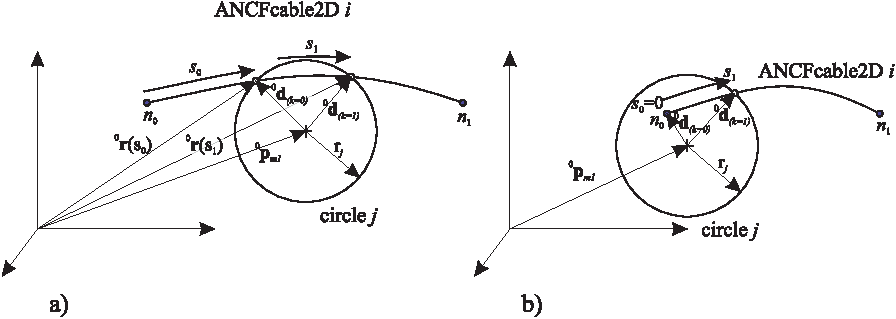
\includegraphics[width=\textwidth]{figures/generalContactANCF2Dcircle}
  \end{center}
  \caption{Geometrical relations for contact of ANCFCable2D $i$ and circle $j$ with according marker $m1$; case a) shows a cable with nodes $n_0$ and $n_1$, partially penetrating at the midspan of the cable; case b) shows the case of a cable where node $n_0$ is inside the cable.}
	\label{fig_generalContactANCF2Dcircle}
\end{figure}
%++++++++++++++++++++++++
\newcommand{\ANCFdk}{\LU{0}{\dv_k}}
\newcommand{\ANCFdkt}{\LU{0}{\dot\dv_k}}
\newcommand{\ANCFdkO}{\LU{0}{\dv_{0,k}}}
\newcommand{\ANCFdkOtp}{\LU{0}{\dv_{0,k}\tp}}
\newcommand{\diffANCFdk}{\diffANCFmI{\ANCFdk}}

Normal contact and tangential friction forces are then computed based on integrals over the coordinates $[s_0,\, s_1]$.
The integration is performed over $n_{ip}$ integration points $x_k \in [x_{i0},\, x_{i1},\, \ldots]$. In case of a 3 point Lobatto integration, we chose the integration points 
\be
  x_k \in [s_0, (s_0+s_1)/2, s_1] \eqDot
\ee
According weights are
\be
  w_k \in [1/3, 4/3, 1/3] \eqDot
\ee
The ANCF cable provides the global position of an integration point $k \in \{i0,\, i1,\, \ldots\}$ via
\be
  \LU{0}{\rv(x_{k})} = \LU{0}{\Sm(x_{k})} \qv
\ee
with ANCF shape function matrix $\Sm$ and current ANCF coordinates $\qv$.
Note that in the simplified case with linear segments, $\LU{0}{\rv(x_{k})}$ is computed from linear interpolation of the segment which is attached to the cable.
The velocity is computed in the same way,
\be
  \LU{0}{\dot \rv(x_{k})} = \LU{0}{\Sm(x_{k})} \dot\qv
\ee
again using linear interpolation of the velocities along the straight segment, if linear segments are used.

In order to perform the integration of contact forces due to penetration as well as tangential (friction) forces, we iterate over all integration points, and sum up the according generalized forces on the cable and the circle marker object.

\noindent The integration factor for integration point $k$ follows from
\be
  f_k = \frac{s_1 - s_0}{2} w_k \eqComma
\ee
assuming axial stretch of the cable element being moderately small.
The vector $\ANCFdk$ which points from the center of the circle to the cable (integration) point reads
\be
  \ANCFdk = \LU{0}{\rv(x_{k})} - \LU{0}{\pv_j} 
\ee
The velocity of the circle at the contact integration point $k$ follows as
\be
  \LU{0}{\vv_{c,k}} = \LU{0}{\vv_j} + \left( \LU{0,m0}{\Am} \LU{m0}{\tomega}_{j} \right) \times \ANCFdk
\ee
The distance $L$ between cable and circle center point, gap $g$ and the contact normal vector read
\be
  L_k = |\ANCFdk|, \quad g= L_k - (r + h_{1/2}), \quad \LU{0}{\dv_{0,k}} = \frac{1}{L_k} \ANCFdk
\ee
with the half height of the ANCF element $h_{1/2}$, which gives additional penetration. Note that this height is added on the side of the circle, which virtually represents a larger circle, behaving slightly different from a cable with thickness $h$.

\noindent The velocity in contact normal direction reads (note that we use the velocity of the circle's center point),
\be
  v_n = \LU{0}{\dv_{0,k}} \left( \LU{0}{\dot \rv(x_{k})} - \LU{0}{\vv}_j \right)
\ee
The contact force (tension! is always negative) follows in the simplistic case of a linear contact model as
\be \label{eq_GeneralContactASfc}
  f_{c,k} = k_c \cdot g  + d \cdot v_n
\ee
with contact stiffness $k_c$ and contact normal damping $d_c$.

\noindent In case of tangential friction, the tangential velocity reads
\bea
  \vv_{t,k} &=& \LU{0}{\dot \rv(x_{k})} - \LU{0}{\vv}_{c,k} - v_n \cdot \LU{0}{\dv_{0,k}}
  = \LU{0}{\dot \rv(x_{k})} - \LU{0}{\vv_j} - \left( \LU{0,m0}{\Am} \LU{m0}{\tomega}_{j} \right) \times \ANCFdk - v_n \cdot \LU{0}{\dv_{0,k}} \nonumber \\
  &=& -\left(\LU{0}{\dv_{0,k}} \otimes \LU{0}{\dv_{0,k}} -\Im \right) \left( \LU{0}{\dot \rv(x_{k})} - \LU{0}{\vv}_{c,k} \right) 
      +\LU{0}{\tilde \dv_k} \LU{0,m0}{\Am} \LU{m0}{\tomega}_{j} 
\eea
and the friction force is computed from \eq{eq_GeneralContactRegularizedFriction} using the contact pressure $-f_{c,k}$ from \eq{eq_GeneralContactASfc}, while otherwise $\LU{0}{\fv_f} = \Null$.

The force vector for the contact point for integration point $k$, including integration weight $f_k$\footnote{this is done, because all further terms are proportional to $\fv_k$.} thus reads
\be
  \LU{0}{\fv_k} = f_k \cdot \left(f_{c,k} \cdot \LU{0}{\dv_{0,k}} + \LU{0}{\fv_f} \right)
\ee
%
The total force and torque on the circle $j$ is found by summation over all integration points $k$,
\be
  \LU{0}{\fv_{circ}} = \sum_k \LU{0}{\fv_{circ,k}}  = \sum_k \LU{0}{\fv_k}, \quad
  \LU{0}{\tv_{circ}} = \sum_k \LU{0}{\tv_{circ,k}}  = \sum_k \left( r_j \cdot \LU{0}{\dv_{0,k}} \right) \times \LU{0}{\fv_k}
\ee
and the contribution to the generalized forces of the ANCF cable element (with generalized coordinates $\qv_{ANCF}$) read
\be
  \fv_{ANCF} = \sum_k \fv_{ANCF,k} = \sum_k \LU{0}{\Sm(x_{k})\tp} \cdot \LU{0}{\fv_k}
\ee
%Note that in the implementation, $f_k$ is already included in the contact force $\fv_k$.
%
The generalized \ac{LHS} forces for marker $m1$ (with generalized coordinates $\qv_{m1}$) thus read
\be
  \fv_{m1,LHS} = \LU{0}{\Jm_{pos,m1}\tp} \LU{0}{\fv_{circ}} + 
                 \LU{0}{\Jm_{rot,m1}\tp} \LU{0}{\tv_{circ}} \eqDot
\ee
The Jacobian matrix for the circle-ANCF contact on position level thus reads\footnote{terms that are implemented are marked in green; black terms are not implemented or unused},
\be
  \termA{
  \Jm_{c}  = \mp{\diffANCF{ \LU{0}{\fv_{ANCF}} }}
                {\diffmI{   \LU{0}{\fv_{ANCF}} }}
                {-\diffANCF{ \left( \LU{0}{\Jm_{pos,m1}\tp} \LU{0}{\fv_{circ}} + \LU{0}{\Jm_{rot,m1}\tp} \LU{0}{\tv_{circ}}\right)}}
                {\diffmI{ \left( \LU{0}{\Jm_{pos,m1}\tp} \LU{0}{\fv_{circ}} + \LU{0}{\Jm_{rot,m1}\tp} \LU{0}{\tv_{circ}}\right)}}
                }
\ee
and on velocity level, it follows as
\be
  \termA{
  \Jm_{c}  = \mp{\diffANCFt{ \LU{0}{\fv_{ANCF}} }}
                {\diffmIt{   \LU{0}{\fv_{ANCF}} }}
                {-\diffANCFt{ \left( \LU{0}{\Jm_{pos,m1}\tp} \LU{0}{\fv_{circ}} + \LU{0}{\Jm_{rot,m1}\tp} \LU{0}{\tv_{circ}}\right)}}
                {\diffmIt{ \left( \LU{0}{\Jm_{pos,m1}\tp} \LU{0}{\fv_{circ}} + \LU{0}{\Jm_{rot,m1}\tp} \LU{0}{\tv_{circ}}\right)}}
                }
\ee
For the calculation of the jacobian, the derivatives of the following terms are needed:
\bi
  \item $\ANCFdk = \LU{0}{\rv(x_{k})} - \LU{0}{\pv_j} $:
  \be
    \diffANCF{\ANCFdk} = \diffANCF{\LU{0}{\rv(x_{k})} - \LU{0}{\pv_j} }
    = \LU{0}{\Sm(x_{k})}
  \ee
  \be
    \diffmI{\ANCFdk} = \diffmI{\LU{0}{\rv(x_{k})} - \LU{0}{\pv_j} }
    = -\LU{0}{\Jm_{pos,m1}}
  \ee
  \item $\ANCFdkt = \LU{0}{\dot \rv(x_{k})} - \LU{0}{\dot \vv_j} $:
  \be
    \diffANCFt{\ANCFdkt} = \diffANCF{\LU{0}{\dot \rv(x_{k})} - \LU{0}{\vv_j} }
    = \LU{0}{\Sm(x_{k})}
  \ee
  \be
    \diffmIt{\ANCFdkt} = \diffmI{\LU{0}{\dot \rv(x_{k})} - \LU{0}{\vv_j} }
    = -\LU{0}{\Jm_{pos,m1}}
  \ee
  \item $L_k = |\ANCFdk| = \left(\LU{0}{\dv_k\tp} \ANCFdk \right) ^{1/2}$:
  \be
    \diffANCFmI{ |\ANCFdk| } = \frac{1}{L_k}\left(\LU{0}{\dv_k\tp} \diffANCFdk \right) =
    \ANCFdkOtp \diffANCFdk 
  \ee
  %\be
    %\diffmI{ |\ANCFdk| } = - \frac{1}{L_k}\left(\LU{0}{\dv_k\tp} \LU{0}{\Jm_{pos,m1}} \right) =
    %-\left(\ANCFdkO\!\tp \LU{0}{\Jm_{pos,m1}} \right) 
  %\ee
  \item $L_k^{-1} = \left(\LU{0}{\dv_k\tp} \ANCFdk \right) ^{-1/2}$ (note different sign as in $L$-term due to $-1/2$):
  \be
    \diffANCFmI{ L_k^{-1} } = \diffANCFmI{\left(\LU{0}{\dv_k\tp} \ANCFdk \right) ^{-1/2} } = 
    -\frac{1}{L_k}\left(\ANCFdkOtp \diffANCFdk \right)
  \ee
  %\be
    %\diffmI{ L_k^{-1} } = \diffmI{\left(\LU{0}{\dv_k\tp} \ANCFdk \right) ^{-1/2} } = 
    %\frac{1}{2\cdot L_k^3}\left(\LU{0}{\dv_k\tp} \LU{0}{\Jm_{pos,m1}} \right)
  %\ee
  %\item $L^{-1} = \left(\LU{0}{\nv}\!\tp\LU{0}{\nv}\right)^{-\frac{1}{2}}$:
  %\be
    %\termC{\frac{\partial L^{-1}}{\partial \qv_{m0}} =
    %\frac{\partial \left(\LU{0}{\nv}\!\tp\LU{0}{\nv}\right)^{-\frac{1}{2}} }{\partial \qv_{m0}} =
    %-\frac{1}{2\cdot L^3}\left(\LU{0}{\nv}\!\tp \frac{\partial \LU{0}{\nv}}{\partial \qv_{m0}} \right) =
    %\frac{1}{2\cdot L^3}\left(\LU{0}{\nv}\!\tp \LU{0}{\Jm_{pos,m0}} \right) }
  %\ee
  \item $\ANCFdkO = \frac{1}{L_k} \ANCFdk$: 
  \be
    \diffANCFmI{ \ANCFdkO } = \diffANCFmI{\frac{1}{L_k} \ANCFdk } = 
    - \frac{1}{L_k^2}\ANCFdk \otimes \left(\ANCFdkOtp \diffANCFdk \right) 
    + \frac{1}{L_k} \diffANCFdk = \frac{1}{L_k} \left(\Im - \ANCFdkO \otimes \ANCFdkO \right) \diffANCFdk
  \ee
  %\be
    %\diffmI{ \ANCFdkO } = \diffmI{\frac{1}{L_k} \ANCFdk } = 
      %\frac{1}{2\cdot L_k^3}\left(\LU{0}{\dv_k\tp} \LU{0}{\Jm_{pos,m1}} \right) \ANCFdk
    %- \frac{1}{L_k} \LU{0}{\Jm_{pos,m1}}
  %\ee
  \item $g= L_k - (r + h_{1/2})$:
  \be
    \diffANCFmI{ g } = \diffANCFmI{ L_k } =
    \ANCFdkOtp \diffANCFdk 
    %\LU{0}{\Sm(x_{k})}
  \ee
  %\be
    %\diffmI{ p } = -\frac{1}{L_k}\left(\ANCFdk\!\tp \LU{0}{\Jm_{pos,m1}} \right) =
    %-\ANCFdkO\!\tp \LU{0}{\Jm_{pos,m1}} 
  %\ee
  %+++++++++++++++++++++++++++++++++++++++++++++++++++++++++++++++++++++++++++++++++++++++++++++++++++++++++
  \item velocity at circle contact point $k$: $\LU{0}{\vv_{c,k}} = \LU{0}{\vv_j} + \left( \LU{0,m1}{\Am} \LU{m1}{\tomega}_{j} \right) \times \ANCFdk = \LU{0}{\vv_j} - \LU{0}{\tilde \dv_k} \LU{0,m1}{\Am} \LU{m1}{\tomega}_{j} $:
  \be
    \diffmIt{ \LU{0}{\vv_{c,k}} } =\LU{0}{\Jm_{pos,m1}}  - \LU{0}{\tilde \dv_k} \LU{0}{\Jm_{rot,m1}}
  \ee
  %+++++++++++++++++++++++++++++++++++++++++++++++++++++++++++++++++++++++++++++++++++++++++++++++++++++++++
  \item $v_n = \ANCFdkO \left( \LU{0}{\dot \rv(x_{k})} - \LU{0}{\vv}_{c,k} \right)$:\footnote{the approximate sign is used, because $\LU{0}{\vv}_{c,k}$ includes a normal component if ANCF cable is not fully tangential, which is not considered here.}
  \be
    \diffANCFmIt{ v_n } = \ANCFdkO \diffANCFt{\left( \LU{0}{\dot \rv(x_{k})} - \LU{0}{\vv}_{c,k} \right) } 
    \approx %because \LU{0}{\vv}_{c,k} includes normal component if ANCF cable is not fully tangential
        \ANCFdkOtp \diffANCFdk
  \ee
  %\be
    %\diffmIt{ v_n } = \ANCFdkO \diffmIt{\left( \LU{0}{\dot \rv(x_{k})} - \LU{0}{\vv}_{c,k} \right) } 
    %\approx -\ANCFdkO \LU{0}{\Jm_{pos,m1}}
  %\ee
  %+++++++++++++++++++++++++++++++++++++++++++++++++++++++++++++++++++++++++++++++++++++++++++++++++++++++++
  \item $\vv_{t,k} = \LU{0}{\dot \rv(x_{k})} - \LU{0}{\vv}_j - v_n \cdot \ANCFdkO =
  \left(\Im - \ANCFdkO \otimes \ANCFdkO \right) \left( \LU{0}{\dot \rv(x_{k})} - \LU{0}{\vv_j} \right) 
      +\LU{0}{\tilde \dv_k} \LU{0}{\tomega}_{j} $:
  \be
    \diffANCFt{\vv_{t,k} } = \left(\Im - \ANCFdkO \otimes \ANCFdkO \right) \LU{0}{\Sm(x_{k})}
  \ee
  \be
    \diffmIt{\vv_{t,k} } = -\left(\Im - \ANCFdkO \otimes \ANCFdkO \right) \LU{0}{\Jm_{pos,m1}} + \LU{0}{\tilde \dv_k} \LU{0}{\Jm_{rot,m1}}
  \ee
  %+++++++++++++++++++++++++++++++++++++++++++++++++++++++++++++++++++++++++++++++++++++++++++++++++++++++++
  \item $f_{c,k} = k_c \cdot g  + d_c \cdot v_n$:
  \be 
    \termA{ \diffANCF{ f_{c,k} } } = \termC{ k_c \cdot \diffANCF{ g } }  + d_c \cdot \diffANCF{ v_n }
    \approx \termC{ k_c \cdot \LU{0}{\dv_{k,0}\tp} \LU{0}{\Sm(x_{k})} }
  \ee
  \be 
    \termA{ \diffmI{ f_{c,k} } } = \termC{ k_c \cdot \diffmI{ p } }  + d_c \cdot \diffmI{ v_n }
    \approx \termC{ -k_c \cdot \LU{0}{\dv_{k,0}\tp} \LU{0}{\Jm_{pos,m1}} }
  \ee
  \be 
    \termC{\diffANCFt{ f_{c,k} } = d_c \cdot \diffANCFt{ v_n } = d_c \cdot \ANCFdkO \LU{0}{\Sm(x_{k})} }
  \ee  
  \be 
    \termC{\diffmIt{ f_{c,k} } = d_c \cdot \diffmIt{ v_n } = -d_c \cdot \ANCFdkO \LU{0}{\Jm_{pos,m1}} }
  \ee  
  %+++++++++++++++++++++++++++++++++++++++++++++++++++++++++++++++++++++++++++++++++++++++++++++++++++++++++
\ei
The contact force reads (note that because $f_c$ is always negative, the sign of regularization term is negative),
\be
  \LU{0}{\fv_k} = f_k \cdot \left( f_{c,k} \cdot \ANCFdkO + \fv_f \right)
                =
              \begin{cases}
                f_k \cdot f_{c,k} \left(\ANCFdkO - \frac{\mu_s}{v_{\mu,reg}}\LU{0}{\vv_t} \right), \quad \mathrm{if} \quad |\LU{0}{\vv_t}| < v_{\mu,reg} \\
                f_k \cdot \left( f_{c,k} \cdot \ANCFdkO + \fv_f \right), \quad \mbox{else with $\fv_f = const.$} 
              \end{cases}
\ee
%++++++++++++++++++++++++++
We introduce a factor $\delta_f$, which is $\delta_f=1$ in the regularized small velocity state, and in the saturated (constant) friction force we use $\delta_f=0$. Thus, the derivative of $\fv_f$, using $|f_{c,k}| = -f_{c,k}$, reads:
  \bea
    \termA{ \diffANCFmIt{\fv_f} } &=& \termA{ \delta_f \frac{\mu_s}{v_{\mu,reg}} \diffANCFmIt{ (-f_{c,k} \LU{0}{\vv_t}) } } \approx
    \termC{ -\delta_f f_{c,k} \frac{\mu_s}{v_{\mu,reg}} \diffANCFmIt{ \LU{0}{\vv_t} } } \nonumber \\
    \termC{ \diffANCFt{\fv_f} } &\approx& \termC{ -\delta_f f_{c,k} \frac{\mu_s}{v_{\mu,reg}} \left(\Im - \ANCFdkO \otimes \ANCFdkO \right) \LU{0}{\Sm(x_{k})} } \nonumber \\
    \termC{ \diffmIt{\fv_f} } &\approx& \termC{ -\delta_f f_{c,k} \frac{\mu_s}{v_{\mu,reg}} \left(-\left(\Im - \ANCFdkO \otimes \ANCFdkO \right) \LU{0}{\Jm_{pos,m1}} + \LU{0}{\tilde \dv_k} \LU{0}{\Jm_{rot,m1}} \right) }
    %+ \LU{0}{\tilde \dv_k} \LU{0}{\Jm_{rot,m1}} \right)
     %\mbox{??? minus in term 3 ???}
  \eea
%
%+++++++++++++++++++++++++++++++++++++++++++++++++++++++++++++++++++++++++++++++++++++++++++++++++++++++++
The term $\LU{0}{\fv_k}$ gives:
  \bea
    \termA{\frac{\partial \LU{0}{\fv_k}}{\partial \qv_{ANCF,m1}} } &=& 
    \termC{f_k \cdot} \left(\termA{ \left(\ANCFdkO - \frac{\mu_s}{v_{\mu,reg}}\LU{0}{\vv_t} \right) \otimes \frac{\partial f_{c,k}}{\partial \qv_{ANCF,m1}} } + 
    f_{c,k} \cdot \frac{\partial \ANCFdkO}{\partial \qv_{ANCF,m1}} +
    \diffANCFmI{\LU{0}{\fv_f}} \right)  \nonumber \\
    &\approx& \termC{f_k \cdot k_c \cdot \left( \left(\ANCFdkO - \frac{\mu_s}{v_{\mu,reg}}\LU{0}{\vv_t} \right) \otimes \ANCFdkO \diffANCFmI{\LU{0}{\dv_{k}}} \right) }
  \eea
and the velocity terms yield
  \bea
    \termA{\diffANCFt{\LU{0}{\fv_k}} } &=& 
    \termC{f_k \cdot \left(d_c \cdot \left(\ANCFdkO - \frac{\mu_s}{v_{\mu,reg}}\LU{0}{\vv_t} \right) \otimes \diffANCFt{v_n}  + 
    \diffANCFt{\LU{0}{\fv_f}} \right) } \nonumber \\
    &\approx& \termC{f_k \cdot \left( d_c \cdot \left(\ANCFdkO - \frac{\mu_s}{v_{\mu,reg}}\LU{0}{\vv_t} \right) \otimes \ANCFdkO -
    \delta_f f_{c,k} \frac{\mu_s}{v_{\mu,reg}} \left(\Im - \ANCFdkO \otimes \ANCFdkO \right) \right)\diffANCFt{\ANCFdkt}  }
  \eea
  \bea
    \termA{\diffmIt{\LU{0}{\fv_k}} } &=& 
    \termC{f_k \cdot \left(d_c \cdot \left(\ANCFdkO - \frac{\mu_s}{v_{\mu,reg}}\LU{0}{\vv_t} \right) \otimes \diffmIt{v_n}  + 
    \diffmIt{\LU{0}{\fv_f}} \right) } \nonumber \\
    &\approx& \termC{f_k \cdot \left( \left( d_c \cdot \left(\ANCFdkO - \frac{\mu_s}{v_{\mu,reg}}\LU{0}{\vv_t} \right) \otimes \ANCFdkO  -
    \delta_f f_{c,k} \frac{\mu_s}{v_{\mu,reg}} \left(\Im - \ANCFdkO \otimes \ANCFdkO\right) \right) \diffmIt{\ANCFdkt}\right.  } \nonumber\\
    && \termC{\left.  + \delta_f f_{c,k} \frac{\mu_s}{v_{\mu,reg}} \LU{0}{\tilde \dv_k} \LU{0}{\Jm_{rot,m1}} \right) }
  \eea
%++++++++++++++++++++++++++
%
The single jacobian terms w.r.t.\ $\qv_{ANCF}$ and $\qv_{m1}$ may be expressed as
%terms with $\diamond$ are neglected in the current implementation}
\bea
  &&\termA{\frac{\partial \left( \LU{0}{\Jm_{pos,m1}\tp} \LU{0}{\fv_{circ}} + \LU{0}{\Jm_{rot,m1}\tp} \LU{0}{\tv_{circ}}\right)}{\partial \qv_{ANCF,m1}}} = \nonumber \\
  &&\frac{\partial \LU{0}{\Jm_{pos,m1}\tp}}{\partial \qv_{ANCF,m1}} \LU{0}{\fv_{circ}}
  +\termC{\LU{0}{\Jm_{pos,m1}\tp}} \termA{\frac{\partial \LU{0}{\fv_{circ}}}{\partial \qv_{ANCF,m1}}}
  +\frac{\partial \LU{0}{\Jm_{rot,m1}\tp}}{\partial \qv_{m0,1}} \LU{0}{\tv_{circ}}
  +\termC{\LU{0}{\Jm_{rot,m1}\tp}} \termA{\frac{\partial \LU{0}{\tv_{circ}}}{\partial \qv_{ANCF,m1}}}
\eea
%\frac{\partial  }{\partial \qv_{ANCF,m1}}
Note that similar relations follow for the time derivatives $\frac{\partial}{\partial \dot \qv_{ANCF,m1}}\left( \right) $.

\noindent The derivatives of $\LU{0}{\fv_{ANCF}}$, $\LU{0}{\fv_{circ}}$, and 
\be
  \LU{0}{\tv_{circ}} = \sum_k r_j \cdot  \ANCFdkO \times \LU{0}{\fv_k} = 
                       \sum_k r_j \cdot  \LU{0}{\tilde \dv_{0,k}} \LU{0}{\fv_k}
\ee
follow from
%\LU{0}{\tv_{circ}} = \sum_k \LU{0}{\tv_{circ,k}}  = \sum_k \left( r_j \cdot \ANCFdkO \right) \times \cdot \LU{0}{\fv_k}
\bea
  \diffANCFmI{\LU{0}{\fv_{ANCF}} } &=& \termC{\sum_k \LU{0}{\Sm(x_{k})\tp}} \termA{\frac{\partial \LU{0}{\fv_k}}{\partial \qv_{ANCF,m1}}}, \nonumber \\
  %\termA{-\LU{0}{\Jm_{pos,m0}\tp} \frac{\partial  \LU{0}{\fv_{ANCF}} }{\partial \qv_{ANCF,m1}}}
  %\termA{\frac{\partial  \LU{0}{\fv_{ANCF}} }{\partial \qv_{ANCF,m1}}} &=& 
  %\termC{\sum_k \LU{0}{\Sm(x_{k})\tp}} \termA{\frac{\partial \LU{0}{\fv_k}}{\partial \qv_{ANCF,m1}}}, \nonumber \\
%
  \termA{\diffANCFmI{ \LU{0}{\fv_{circ}} } } &=& \termA{ \sum_k \diffANCFmI{ \LU{0}{\fv_k} } }, \nonumber \\
%
  \termA{\frac{\partial  \LU{0}{\tv_{circ}} }{\partial \qv_{ANCF,m1}}} &\approx& 
  \sum_k \left( \termC{r_j \cdot  \LU{0}{\tilde \dv_{0,k}} } \termA{\diffANCFmI{\LU{0}{\fv_k}} } - 
                r_j \cdot \LU{0}{\tilde \fv_k} \diffANCFmI{\LU{0}{\dv_{0,k}} } \right)
\eea


%+++++++++++++++++++++++++++++++++++++++++++++++++++++++++++++++++++++++++++++++++++++++++++++++++
    %\mysubsubsubsection{Connector forces}
    %%
    %The unit vector in force direction reads (raises SysError if $L=0$),
    %\be
      %\vv_{f} = \frac{1}{L} \Delta\! \LU{0}{\pv}
    %\ee
    %If \texttt{activeConnector = True}, the scalar spring force is computed as
    %\be
      %f_{SD} = k\cdot(L-L_0) + d \cdot\Delta\! \LU{0}{\vv}\tp \vv_{f} + f_{a}
    %\ee
    %If the springForceUserFunction $\mathrm{UF}$ is defined, $\fv$ instead becomes ($t$ is current time)
    %\be
      %f_{SD} = \mathrm{UF}(mbs, t, i_N, L-L_0, \Delta\! \LU{0}{\vv}\tp \vv_{f}, k, d, f_{a})
    %\ee
    %and \texttt{iN} represents the itemNumber (=objectNumber). Note that, if \texttt{activeConnector = False}, $f_{SD}$ is set to zero.
%
    %The vector of the spring-damper force applied at both markers finally reads
    %\be
      %\fv = f_{SD}\vv_{f}
    %\ee
    %The virtual work of the connector force is computed from the virtual displacement 
    %\be
      %\delta \Delta\! \LU{0}{\pv} = \delta \LU{0}{\pv}_{m1} - \delta \LU{0}{\pv}_{m0} \eqComma
    %\ee
    %and the virtual work (not the transposed version here, because the resulting generalized forces shall be a column vector,
    %\be
      %\delta W_{SD} = \fv \delta \Delta\! \LU{0}{\pv} 
      %= \left( k\cdot(L-L_0) + d \cdot\Delta\! \LU{0}{\vv}\tp \vv_{f} + f_{a} \right) \left(\delta \LU{0}{\pv}_{m1} - \delta \LU{0}{\pv}_{m0} \right)\tp \vv_{f} 
      %\eqDot
    %\ee
    %The generalized (elastic) forces thus result from
    %\be
      %\Qm_{SD} = \frac{\partial \LU{0}{\pv}}{\partial \qv_{SD}\tp} \fv 
      %\eqComma
    %\ee
    %and read for the markers $m0$ and $m1$,
    %\be
      %\Qm_{SD, m0} 
      %= -\left( k\cdot(L-L_0) + d \cdot\Delta\! \LU{0}{\vv}\tp \vv_{f} + f_{a} \right) \Jm_{pos,m0}\tp \vv_{f} , \quad
      %\Qm_{SD, m1} 
      %= \left( k\cdot(L-L_0) + d \cdot\Delta\! \LU{0}{\vv}\tp \vv_{f} + f_{a} \right) \Jm_{pos,m1}\tp \vv_{f} 
      %\eqComma    
    %\ee
    %where $\Jm_{pos,m1}$ represents the derivative of marker $m1$ w.r.t.\ its associated coordinates $\qv_{m1}$, analogously $\Jm_{pos,m0}$.
    %%
    %\mysubsubsubsection{Connector Jacobian}
    %The position-level jacobian for the connector, involving all coordinates associated with markers $m0$ and $m1$, follows from 
    %\be
      %\Jm_{SD} = \mp{\frac{\partial \Qm_{SD, m0}}{\partial \qv_{m0}} }{\frac{\partial \Qm_{SD, m0}}{\partial \qv_{m1}}}
                    %{\frac{\partial \Qm_{SD, m0}}{\partial \qv_{m1}} }{\frac{\partial \Qm_{SD, m1}}{\partial \qv_{m1}}}
    %\ee
    %and the velocity level jacobian reads
    %\be
      %\Jm_{SD,t} = \mp{\frac{\partial \Qm_{SD, m0}}{\partial \dot \qv_{m0}} }{\frac{\partial \Qm_{SD, m0}}{\partial \dot \qv_{m1}}}
                    %{\frac{\partial \Qm_{SD, m0}}{\partial \dot \qv_{m1}} }{\frac{\partial \Qm_{SD, m1}}{\partial \dot \qv_{m1}}}
    %\ee
    %The sub-Jacobians follow from
    %\be
      %\frac{\partial \Qm_{SD, m0}}{\partial \qv_{m0}} = 
       %-\frac{\partial \Jm_{pos,m0}\tp }{\partial \qv_{m0}} \vv_{f} \left( k\cdot(L-L_0) + d \cdot\Delta\! \LU{0}{\vv}\tp \vv_{f} + f_{a} \right) 
       %-\Jm_{pos,m0}\tp \frac{\partial \vv_{f} \left( k\cdot(L-L_0) + d \cdot\Delta\! \LU{0}{\vv}\tp \vv_{f} + f_{a} \right)   }{\partial \qv_{m0}} 
    %\ee
    %in which the term $\frac{\partial \Jm_{pos,m0}\tp }{\partial \dot \qv_{m0}}$ is computed from a special function provided by markers, that
    %compute the derivative of the marker jacobian times a constant vector, in this case the spring force $\fv$; this jacobian term is usually less  
    %dominant, but is included in the numerical as well as the analytical derivatives, see the general jacobian computation information.
    %
    %The other term, which is the dominant term, is computed as (dependence of velocity term on position coordinates neglected),
    %\bea
      %\frac{\partial \Qm_{SD, m0}}{\partial \qv_{m0}}
      %&=& -\Jm_{pos,m0}\tp \frac{\partial \vv_{f} \left( k\cdot(L-L_0) + d \cdot\Delta\! \LU{0}{\vv}\tp \vv_{f} + f_{a} \right)   }{\partial \qv_{m0}}
      %\nonumber \\
      %&=& -\Jm_{pos,m0}\tp \frac{\partial  \left( k\cdot \left( \Delta\! \LU{0}{\pv} - L_0 \vv_{f} \right)+ \vv_{f} \left(d \cdot \vv_{f}\tp \Delta\! \LU{0}{\vv}  + f_{a} \right) \right)   }{\partial \qv_{m0}} 
      %\nonumber \\
      %&\approx& \Jm_{pos,m0}\tp \left(k\cdot \Im - k  \frac{L_0}{L}\left(\Im - \LU{0}{\vv_{f}} \otimes \LU{0}{\vv_{f}} \right)  +\frac{1}{L}\left(\Im - \LU{0}{\vv_{f}} \otimes \LU{0}{\vv_{f}} \right) \left(d \cdot \vv_{f}\tp \Delta\! \LU{0}{\vv}  + f_{a} \right) \right)
      %\LU{0}{\Jm_{pos,m0}}
    %\eea
    %Noting that $\frac{\partial \vv_{f} }{\partial \qv_{m0}} = 
    %-\frac{1}{L}\left(\Im - \LU{0}{\vv_{f}} \otimes \LU{0}{\vv_{f}} \right) \LU{0}{\Jm_{pos,m0}}$ and 
    %$\frac{\partial \vv_{f} }{\partial \qv_{m1}} = 
    %\frac{1}{L}\left(\Im - \LU{0}{\vv_{f}} \otimes \LU{0}{\vv_{f}} \right) \LU{0}{\Jm_{pos,m1}}$.
%%
    %The Jacobian w.r.t.\ velocity coordinates follows as
    %\bea
      %\frac{\partial \Qm_{SD, m0}}{\partial \dot \qv_{m0}}
      %&=& -\Jm_{pos,m0}\tp \frac{\partial \vv_{f} \left( k\cdot(L-L_0) + d \cdot\Delta\! \LU{0}{\vv}\tp \vv_{f} + f_{a} \right)   }{\partial \dot \qv_{m0}}
      %\nonumber \\
      %&=& \Jm_{pos,m0}\tp \left(d \vv_{f} \otimes \vv_{f} \right) \LU{0}{\Jm_{pos,m0}} 
    %\eea
    %Jacobians for markers $m1$ and mixed $m0$/$m1$ terms follow analogously.
    

}

\iftoggle{compileAll}
{
% ++++++++++++++++++++++
% description of manual pybind interfaces; generated by Johannes Gerstmayr
% ++++++++++++++++++++++

\mysection{Python-C++ command interface}
\label{sec:PCpp:command:interface}

This chapter lists the basic interface functions which can be used to set up a \codeName\ model in Python.

\mysubsection{General information on Python-C++ interface}
\label{sec:generalPythonInterface}
This chapter lists the basic interface functions which can be used to set up 
a \codeName\ model in Python. Note that some functions or classes will be used in examples, which are explained in detail later on.
In the following, some basic steps and concepts for usage are shown, references to all functions are placed hereafter:

To import the module, just include the \codeName\ module in Python:
\pythonstyle
\begin{lstlisting}[language=Python, firstnumber=1]

import exudyn as exu
\end{lstlisting}


For compatibility with examples and other users, we recommend to use the \texttt{exu} abbreviation throughout. In addition, you may work with a convenient interface for your items, therefore also always include:
\pythonstyle
\begin{lstlisting}[language=Python, firstnumber=1]

from exudyn.itemInterface import *
\end{lstlisting}


Note that including \texttt{exudyn.utilities} will cover \texttt{itemInterface}. Also note that \texttt{from ... import *} is not recommended in general and it will not work in certain cases, e.g., if you like to compute on a cluster. However, it greatly simplifies life for smaller models and you may replace imports in your files afterwards by removing the star import.

The general hub to multibody dynamics models is provided by the classes \texttt{SystemContainer} and \texttt{MainSystem}, except for some very basic system functionality (which is inside the \codeName\ module). 

You can create a new \texttt{SystemContainer}, which is a class that is initialized by assigning a system container to a variable, usually denoted as \texttt{SC}:
\pythonstyle
\begin{lstlisting}[language=Python, firstnumber=1]

SC = exu.SystemContainer()
\end{lstlisting}


Note that creating a second \texttt{exu.SystemContainer()} will be independent of \texttt{SC} and therefore makes no sense if you do not intend to work with two different containers.

To add a MainSystem to system container \texttt{SC} and store as variable \texttt{mbs}, write:
\pythonstyle
\begin{lstlisting}[language=Python, firstnumber=1]

mbs = SC.AddSystem()
\end{lstlisting}


Furthermore, there are a couple of commands available directly in the \texttt{exudyn} module, given in the following subsections. Regarding the \mybold{(basic) module access}, functions are related to the \texttt{exudyn = exu} module, see these examples:
\pythonstyle
\begin{lstlisting}[language=Python, firstnumber=1]

#  import exudyn module:
import exudyn as exu
#  print detailed exudyn version, Python version (at which it is compiled):
exu.GetVersionString(addDetails = True)
#  set precision of C++ output to console
exu.SetOutputPrecision(numberOfDigits)
#  turn on/off output to console
exu.SetWriteToConsole(False)
#  invalid index, may depend on compilation settings:
nInvalid = exu.InvalidIndex() #the invalid index, depends on architecture and version
\end{lstlisting}


Understanding the usage of functions for python object \texttt{SystemContainer} of the module \texttt{exudyn}, the following examples might help:
\pythonstyle
\begin{lstlisting}[language=Python, firstnumber=1]

#import exudyn module:
import exudyn as exu
#  import utilities (includes itemInterface, basicUtilities, 
#                  advancedUtilities, rigidBodyUtilities, graphicsDataUtilities):
from exudyn.utilities import *
#  create system container and store in SC:
SC = exu.SystemContainer()
#  add a MainSystem (multibody system) to system container SC and store as mbs:
mbs = SC.AddSystem()
#  add a second MainSystem to system container SC and store as mbs2:
mbs2 = SC.AddSystem()
#  print number of systems available:
nSys = SC.NumberOfSystems()
exu.Print(nSys) #or just print(nSys)
#  delete reference to mbs and mbs2 (usually not necessary):
del mbs, mbs2
#  reset system container (mbs becomes invalid):
SC.Reset()
\end{lstlisting}


If you run a parameter variation (check \texttt{Examples/parameterVariationExample.py}), you may reset or delete the created \texttt{MainSystem} \texttt{mbs} and the \texttt{SystemContainer} \texttt{SC} before creating new instances in order to avoid memory growth.

\mysubsubsection{Item index}
\label{sec:itemIndex}
Many functions will work with node numbers (\texttt{NodeIndex}), object numbers (\texttt{ObjectIndex}),marker numbers (\texttt{MarkerIndex}) and others. These numbers are special Python objects, which have been introduced in order to avoid mixing up, e.g., node and object numbers. 

For example, the command \texttt{mbs.AddNode(...)} returns a \texttt{NodeIndex}. For these indices, the following rules apply:
\bi
  \item[] \texttt{mbs.Add[Node|Object|...](...)} returns a specific \texttt{NodeIndex}, \texttt{ObjectIndex}, ...
  \item[] You can create any item index, e.g., using \texttt{ni = NodeIndex(42)} or \texttt{oi = ObjectIndex(42)}
  \item[] The benefit of these indices comes as they may not be mixed up, e.g., using an object index instead of a node index.
  \item[] You can convert any item index, e.g., NodeIndex \texttt{ni} into an integer number using \texttt{int(ni)} of \texttt{ni.GetIndex()}
  \item[] Still, you can use integers as initialization for item numbers, e.g.:\\\texttt{mbs.AddObject(MassPoint(nodeNumber=13, ...))}\\However, it must be a pure integer type.
  \item[] You can make integer calculations with such indices, e.g., \texttt{oi = 2*ObjectIndex(42)+1} restricing to addition, subtraction and multiplication. Currently, the result of such calculations is a \texttt{int} type andoperating on mixed indices is not checked (but may raise exceptions in future).
  \item[] You can also print item indices, e.g., \texttt{print(ni)} as it converts to string by default.
  \item[] If you are unsure about the type of an index, use \texttt{ni.GetTypeString()} to show the index type.
\ei
\mysubsubsection{Copying and referencing C++ objects}
\label{sec:generalPythonInterface:copyref}
As a key concept to working with \codeName\ , most data which is retrieved by C++ interface functions is copied.
Experienced Python users may know that it is a key concept to Python to often use references instead of copying, which is
sometimes error-prone but offers a computationally efficient behavior.
There are only a few very important cases where data is referenced in \codeName\ , the main ones are 
\texttt{SystemContainer}, 
\texttt{MainSystem}, 
\texttt{VisualizationSettings}, and
\texttt{SimulationSettings} which are always references to internal C++ classes.
The following code snippets and comments should explain this behavior:
\pythonstyle
\begin{lstlisting}[language=Python, firstnumber=1]

#create system container, referenced from SC:
SC = exu.SystemContainer()
SC2 = SC                           #this will only put a reference to SC
                                   #SC2 and SC represent the SAME C++ object
#add a MainSystem (multibody system):
mbs = SC.AddSystem()               #get reference mbs to C++ system
mbs2=mbs                           #again, mbs2 and mbs refer to the same C++ object
og = mbs.AddObject(ObjectGround()) #copy data of ObjectGround() into C++
o0 = mbs.GetObject(0)              #get copy of internal data as dictionary
del o0                             #delete the local dictionary; C++ data not affected
del mbs, mbs2                      #references to mbs deleted (C++ data still available)
del SC                             #references to SystemContainer deleted
#at this point, mbs and SC are not available any more (data may be cleaned up by Python)
\end{lstlisting}


\mysubsubsection{Exceptions and Error Messages}
\label{sec:cinterface:exceptions}
There are several levels of type and argument checks, leading to different types of errors and exceptions. The according error messages are non-unique, because they may be raised in Python modules or in C++, and they may be raised on different levels of the code. Error messages depend on Python version and on your iPython console. Very often the exception may be called \texttt{ValueError}, but it mustnot mean that it is a wrong error, but it could also be, e.g., a wrong order of function calls.

As an example, a type conversion error is raised when providing wrong argument types, e.g., try \texttt{exu.GetVersionString('abc')}:
\pythonstyle
\begin{lstlisting}[language=Python, firstnumber=1]

Traceback (most recent call last):

File "C:\Users\username\AppData\Local\Temp\ipykernel_24988\2212168679.py", line 1, in <module>
    exu.GetVersionString('abc')

TypeError: GetVersionString(): incompatible function arguments. The following argument types are supported:
    1. (addDetails: bool = False) -> str

Invoked with: 'abc'
\end{lstlisting}


Note that your particular error message may be different.

Another error results from internal type and range checking, saying User ERROR, as it is due to a wrong input of the user. For this, we try
\pythonstyle
\begin{lstlisting}[language=Python, firstnumber=1]
mbs.AddObject('abc')
\end{lstlisting}


Which results in a error message similar to:
\pythonstyle
\begin{lstlisting}[language=Python, firstnumber=1]

=========================================
User ERROR [file 'C:\Users\username\AppData\Local\Temp\ipykernel_24988\2838049308.py', line 1]: 
Error in AddObject(...):
Check your python code (negative indices, invalid or undefined parameters, ...)

=========================================

Traceback (most recent call last):

  File "C:\Users\username\AppData\Local\Temp\ipykernel_24988\2838049308.py", line 1, in <module>
    mbs.AddObject('abc')

RuntimeError: Exudyn: parsing of Python file terminated due to Python (user) error
\end{lstlisting}


Finally, there may be system errors. They may be caused due to previous wrong input, but if there is no reason seen, it may be appropriate to report this error on \exuUrl{https://github.com/jgerstmayr/EXUDYN}{github.com/jgerstmayr/EXUDYN/} .

Be careful in reading and interpreting such error messages. You should \mybold{read them from top to bottom}, as the cause may be in the beginning. Often files and line numbers of errors are provided (e.g., if you have a longer script). In the ultimate case, try to comment parts of your code or deactivate items to see where the error comes from. See also section on Trouble shooting and FAQ.

%++++++++++++++++++++
\mysubsection{\codeName}



These are the access functions to the \codeName\ module. General usage is explained in \refSection{sec:generalPythonInterface} and examples are provided there. The C++ module \texttt{exudyn} is the root level object linked between Python and C++.In the installed site-packages, the according file is usually denoted as \texttt{exudynCPP.pyd} for the regular module, \texttt{exudynCPPfast.pyd} for the module without range checks and \texttt{exudynCPPnoAVX.pyd} for the module compiled without AVX vector extensions (may depend on your installation).
\pythonstyle
\begin{lstlisting}[language=Python, firstnumber=1]

#import exudyn module:
import exudyn as exu
#create systemcontainer and mbs:
SC = exu.SystemContainer()
mbs = SC.AddSystem()
\end{lstlisting}

\begin{center}
\footnotesize
\begin{longtable}{| p{8cm} | p{8cm} |} 
\hline
{\bf function/structure name} & {\bf description}\\ \hline
  GetVersionString(addDetails = False) & Get Exudyn built version as string (if addDetails=True, adds more information on compilation Python version, platform, etc.; the Python micro version may differ from that you are working with; AVX2 shows that you are running a AVX2 compiled version)\\ \hline 
  Help() & Show basic help information\\ \hline 
  RequireVersion(requiredVersionString) & Checks if the installed version is according to the required version. Major, micro and minor version must agree the required level. This function is defined in the \texttt{\_\_init\_\_.py} file\tabnewline 
    \textcolor{steelblue}{{\bf EXAMPLE}: \tabnewline 
    \texttt{exu.RequireVersion("1.0.31")}}\\ \hline 
  StartRenderer(verbose = 0) & Start OpenGL rendering engine (in separate thread) for visualization of rigid or flexible multibody system; use verbose=1 to output information during OpenGL window creation; verbose=2 produces more output and verbose=3 gives a debug level; some of the information will only be seen in windows command (powershell) windows or linux shell, but not inside iPython of e.g. Spyder\\ \hline 
  StopRenderer() & Stop OpenGL rendering engine\\ \hline 
  IsRendererActive() & returns True if GLFW renderer is available and running; otherwise False\\ \hline 
  DoRendererIdleTasks(waitSeconds = 0) & Call this function in order to interact with Renderer window; use waitSeconds in order to run this idle tasks while animating a model (e.g. waitSeconds=0.04), use waitSeconds=0 without waiting, or use waitSeconds=-1 to wait until window is closed\\ \hline 
  SolveStatic(mbs, simulationSettings = exudyn.SimulationSettings(), updateInitialValues = False, storeSolver = True) & Static solver function, mapped from module \texttt{solver}, to solve static equations (without inertia terms) of constrained rigid or flexible multibody system; for details on the Python interface see \refSection{sec:solver:SolveStatic}; for background on solvers, see \refSection{sec:solvers}\\ \hline 
  SolveDynamic(mbs, simulationSettings = exudyn.SimulationSettings(), solverType = exudyn.DynamicSolverType.GeneralizedAlpha, updateInitialValues = False, storeSolver = True) & Dynamic solver function, mapped from module \texttt{solver}, to solve equations of motion of constrained rigid or flexible multibody system; for details on the Python interface see \refSection{sec:solver:SolveDynamic}; for background on solvers, see \refSection{sec:solvers}\\ \hline 
  ComputeODE2Eigenvalues(mbs, simulationSettings = exudyn.SimulationSettings(), useSparseSolver = False, numberOfEigenvalues = -1, setInitialValues = True, convert2Frequencies = False) & Simple interface to scipy eigenvalue solver for eigenvalue analysis of the second order differential equations part in mbs, mapped from module \texttt{solver}; for details on the Python interface see \refSection{sec:solver:ComputeODE2Eigenvalues}\\ \hline 
  SetOutputPrecision(numberOfDigits) & Set the precision (integer) for floating point numbers written to console (reset when simulation is started!); NOTE: this affects only floats converted to strings inside C++ exudyn; if you print a float from Python, it is usually printed with 16 digits; if printing numpy arrays, 8 digits are used as standard, to be changed with numpy.set\_printoptions(precision=16); alternatively convert into a list\\ \hline 
  SetLinalgOutputFormatPython(flagPythonFormat) & True: use Python format for output of vectors and matrices; False: use matlab format\\ \hline 
  SetWriteToConsole(flag) & set flag to write (True) or not write to console; default = True\\ \hline 
  SetWriteToFile(filename, flagWriteToFile = True, flagAppend = False) & set flag to write (True) or not write to console; default value of flagWriteToFile = False; flagAppend appends output to file, if set True; in order to finalize the file, write \texttt{exu.SetWriteToFile('', False)} to close the output file\tabnewline 
    \textcolor{steelblue}{{\bf EXAMPLE}: \tabnewline 
    \texttt{exu.SetWriteToConsole(False) \#no output to console\tabnewline
    exu.SetWriteToFile(filename={\textquotesingle}testOutput.log{\textquotesingle}, flagWriteToFile=True, flagAppend=False)\tabnewline
    exu.Print({\textquotesingle}print this to file{\textquotesingle})\tabnewline
    exu.SetWriteToFile({\textquotesingle}{\textquotesingle}, False) \#terminate writing to file which closes the file}}\\ \hline 
  SetPrintDelayMilliSeconds(delayMilliSeconds) & add some delay (in milliSeconds) to printing to console, in order to let Spyder process the output; default = 0\\ \hline 
  Print(*args) & this allows printing via exudyn with similar syntax as in Python print(args) except for keyword arguments: print('test=',42); allows to redirect all output to file given by SetWriteToFile(...); does not output in case that SetWriteToConsole is set to False\\ \hline 
  SuppressWarnings(flag) & set flag to suppress (=True) or enable (=False) warnings\\ \hline 
  InfoStat(writeOutput = True) & Retrieve list of global information on memory allocation and other counts as list:[array\_new\_counts, array\_delete\_counts, vector\_new\_counts, vector\_delete\_counts, matrix\_new\_counts, matrix\_delete\_counts, linkedDataVectorCast\_counts]; May be extended in future; if writeOutput==True, it additionally prints the statistics; counts for new vectors and matrices should not depend on numberOfSteps, except for some objects such as ObjectGenericODE2 and for (sensor) output to files; Not available if code is compiled with \_\_FAST\_EXUDYN\_LINALG flag\\ \hline 
  Go() & Creates a SystemContainer SC and a main multibody system mbs\\ \hline 
  InvalidIndex() & This function provides the invalid index, which may depend on the kind of 32-bit, 64-bit signed or unsigned integer; e.g. node index or item index in list; currently, the InvalidIndex() gives -1, but it may be changed in future versions, therefore you should use this function\\ \hline 
  variables & this dictionary may be used by the user to store exudyn-wide data in order to avoid global Python variables; usage: exu.variables["myvar"] = 42 \\ \hline  
  sys & this dictionary is used and reserved by the system, e.g. for testsuite, graphics or system function to store module-wide data in order to avoid global Python variables; the variable exu.sys['renderState'] contains the last render state after exu.StopRenderer() and can be used for subsequent simulations \\ \hline  
\end{longtable}
\end{center}

%++++++++++++++++++++
\mysubsection{SystemContainer}



The SystemContainer is the top level of structures in \codeName. The container holds all (multibody) systems, solvers and all other data structures for computation. A SystemContainer is created by \texttt{SC = exu.SystemContainer()}, understanding \texttt{exu.SystemContainer} as a class like Python's internal list class, creating a list instance with \texttt{x=list()}. Currently, only one container shall be used. In future, multiple containers might be usable at the same time. Regarding the \mybold{(basic) module access}, functions are related to the \texttt{exudyn = exu} module, see also the introduction of this chapter and this example:
\pythonstyle
\begin{lstlisting}[language=Python, firstnumber=1]

import exudyn as exu
#create system container and store by reference in SC:
SC = exu.SystemContainer() 
#add MainSystem to SC:
mbs = SC.AddSystem()
\end{lstlisting}

\begin{center}
\footnotesize
\begin{longtable}{| p{8cm} | p{8cm} |} 
\hline
{\bf function/structure name} & {\bf description}\\ \hline
  Reset() & delete all multibody systems and reset SystemContainer (including graphics); this also releases SystemContainer from the renderer, which requires SC.AttachToRenderEngine() to be called in order to reconnect to rendering; a safer way is to delete the current SystemContainer and create a new one (SC=SystemContainer() )\\ \hline 
  AddSystem() & add a new computational system\\ \hline 
  NumberOfSystems() & obtain number of multibody systems available in system container\\ \hline 
  GetSystem(systemNumber) & obtain multibody systems with index from system container\\ \hline 
  visualizationSettings & this structure is read/writeable and contains visualization settings, which are immediately applied to the rendering window. \tabnewline
    EXAMPLE:\tabnewline
    SC = exu.SystemContainer()\tabnewline
    SC.visualizationSettings.autoFitScene=False  \\ \hline  
  GetRenderState() & Get dictionary with current render state (openGL zoom, modelview, etc.); will have no effect if GLFW\_GRAPHICS is deactivated\tabnewline 
    \textcolor{steelblue}{{\bf EXAMPLE}: \tabnewline 
    \texttt{SC = exu.SystemContainer()\tabnewline
    renderState = SC.GetRenderState() \tabnewline
    print(renderState[{\textquotesingle}zoom{\textquotesingle}])}}\\ \hline 
  SetRenderState(renderState) & Set current render state (openGL zoom, modelview, etc.) with given dictionary; usually, this dictionary has been obtained with GetRenderState; will have no effect if GLFW\_GRAPHICS is deactivated\tabnewline 
    \textcolor{steelblue}{{\bf EXAMPLE}: \tabnewline 
    \texttt{SC = exu.SystemContainer()\tabnewline
    SC.SetRenderState(renderState)}}\\ \hline 
  RedrawAndSaveImage() & Redraw openGL scene and save image (command waits until process is finished)\\ \hline 
  WaitForRenderEngineStopFlag() & Wait for user to stop render engine (Press 'Q' or Escape-key); this command is used to have active response of the render window, e.g., to open the visualization dialog or use the right-mouse-button; behaves similar as mbs.WaitForUserToContinue()\\ \hline 
  RenderEngineZoomAll() & Send zoom all signal, which will perform zoom all at next redraw request\\ \hline 
  AttachToRenderEngine() & Links the SystemContainer to the render engine, such that the changes in the graphics structure drawn upon updates, etc.; done automatically on creation of SystemContainer; return False, if no renderer exists (e.g., compiled without GLFW) or cannot be linked (if other SystemContainer already linked)\\ \hline 
  DetachFromRenderEngine() & Releases the SystemContainer from the render engine; return True if successfully released, False if no GLFW available or detaching failed\\ \hline 
  SendRedrawSignal() & This function is used to send a signal to the renderer that all MainSystems (mbs) shall be redrawn\\ \hline 
  GetCurrentMouseCoordinates(useOpenGLcoordinates = False) & Get current mouse coordinates as list [x, y]; x and y being floats, as returned by GLFW, measured from top left corner of window; use GetCurrentMouseCoordinates(useOpenGLcoordinates=True) to obtain OpenGLcoordinates of projected plane\\ \hline 
\end{longtable}
\end{center}

%++++++++++++++++++++
\mysubsection{MainSystem}



This is the class which defines a (multibody) system. The MainSystem shall only be created by \texttt{SC.AddSystem()}, not with \texttt{exu.MainSystem()}, as the latter one would not be linked to a SystemContainer. In C++, there is a MainSystem (the part which links to Python) and a System (computational part). For that reason, the name is MainSystem on the Python side, but it is often just called 'system'. For compatibility, it is recommended to denote the variable holding this system as mbs, the multibody dynamics system. It can be created, visualized and computed. Use the following functions for system manipulation.
\pythonstyle
\begin{lstlisting}[language=Python, firstnumber=1]

import exudyn as exu
SC = exu.SystemContainer()
mbs = SC.AddSystem()
\end{lstlisting}

\begin{center}
\footnotesize
\begin{longtable}{| p{8cm} | p{8cm} |} 
\hline
{\bf function/structure name} & {\bf description}\\ \hline
  Assemble() & assemble items (nodes, bodies, markers, loads, ...) of multibody system; Calls CheckSystemIntegrity(...), AssembleCoordinates(), AssembleLTGLists(), AssembleInitializeSystemCoordinates(), and AssembleSystemInitialize()\\ \hline 
  AssembleCoordinates() & assemble coordinates: assign computational coordinates to nodes and constraints (algebraic variables)\\ \hline 
  AssembleLTGLists() & build \ac{LTG} coordinate lists for objects (used to build global ODE2RHS, MassMatrix, etc. vectors and matrices) and store special object lists (body, connector, constraint, ...)\\ \hline 
  AssembleInitializeSystemCoordinates() & initialize all system-wide coordinates based on initial values given in nodes\\ \hline 
  AssembleSystemInitialize() & initialize some system data, e.g., generalContact objects (searchTree, etc.)\\ \hline 
  Reset() & reset all lists of items (nodes, bodies, markers, loads, ...) and temporary vectors; deallocate memory\\ \hline 
  GetSystemContainer() & return the systemContainer where the mainSystem (mbs) was created\\ \hline 
  WaitForUserToContinue(printMessage = True) & interrupt further computation until user input --> 'pause' function; this command runs a loop in the background to have active response of the render window, e.g., to open the visualization dialog or use the right-mouse-button; behaves similar as SC.WaitForRenderEngineStopFlagthis()\\ \hline 
  SendRedrawSignal() & this function is used to send a signal to the renderer that the scene shall be redrawn because the visualization state has been updated\\ \hline 
  GetRenderEngineStopFlag() & get the current stop simulation flag; True=user wants to stop simulation\\ \hline 
  SetRenderEngineStopFlag(stopFlag) & set the current stop simulation flag; set to False, in order to continue a previously user-interrupted simulation\\ \hline 
  ActivateRendering(flag = True) & activate (flag=True) or deactivate (flag=False) rendering for this system\\ \hline 
  SetPreStepUserFunction(value) & Sets a user function PreStepUserFunction(mbs, t) executed at beginning of every computation step; in normal case return True; return False to stop simulation after current step\tabnewline 
    \textcolor{steelblue}{{\bf EXAMPLE}: \tabnewline 
    \texttt{def PreStepUserFunction(mbs, t):\tabnewline
     \phantom{XXXX} print(mbs.systemData.NumberOfNodes())\tabnewline
     \phantom{XXXX} if(t>1): \tabnewline
     \phantom{XXXX}  \phantom{XXXX} return False \tabnewline
     \phantom{XXXX} return True \tabnewline
     mbs.SetPreStepUserFunction(PreStepUserFunction)}}\\ \hline 
  SetPostNewtonUserFunction(value) & Sets a user function PostNewtonUserFunction(mbs, t) executed after successful Newton iteration in implicit or static solvers and after step update of explicit solvers, but BEFORE PostNewton functions are called by the solver; function returns list [discontinuousError, recommendedStepSize], containing a error of the PostNewtonStep, which is compared to [solver].discontinuous.iterationTolerance. The recommendedStepSize shall be negative, if no recommendation is given, 0 in order to enforce minimum step size or a specific value to which the current step size will be reduced and the step will be repeated; use this function, e.g., to reduce step size after impact or change of data variables\tabnewline 
    \textcolor{steelblue}{{\bf EXAMPLE}: \tabnewline 
    \texttt{def PostNewtonUserFunction(mbs, t):\tabnewline
     \phantom{XXXX} if(t>1): \tabnewline
     \phantom{XXXX}  \phantom{XXXX} return [0, 1e-6] \tabnewline
     \phantom{XXXX} return [0,0] \tabnewline
     mbs.SetPostNewtonUserFunction(PostNewtonUserFunction)}}\\ \hline 
  AddGeneralContact() & add a new general contact, used to enable efficient contact computation between objects (nodes or markers)\\ \hline 
  GetGeneralContact(generalContactNumber) & get read/write access to GeneralContact with index generalContactNumber stored in mbs; Examples shows how to access the GeneralContact object added with last AddGeneralContact() command:\tabnewline 
    \textcolor{steelblue}{{\bf EXAMPLE}: \tabnewline 
    \texttt{gc=mbs.GetGeneralContact(mbs.NumberOfGeneralContacts()-1)}}\\ \hline 
  DeleteGeneralContact(generalContactNumber) & delete GeneralContact with index generalContactNumber in mbs; other general contacts are resorted (index changes!)\\ \hline 
  NumberOfGeneralContacts() & Return number of GeneralContact objects in mbs\\ \hline 
  \_\_repr\_\_() & return the representation of the system, which can be, e.g., printed\tabnewline 
    \textcolor{steelblue}{{\bf EXAMPLE}: \tabnewline 
    \texttt{print(mbs)}}\\ \hline 
  systemIsConsistent & this flag is used by solvers to decide, whether the system is in a solvable state; this flag is set to False as long as Assemble() has not been called; any modification to the system, such as Add...(), Modify...(), etc. will set the flag to False again; this flag can be modified (set to True), if a change of e.g.~an object (change of stiffness) or load (change of force) keeps the system consistent, but would normally lead to systemIsConsistent=False\\ \hline  
  interactiveMode & set this flag to True in order to invoke a Assemble() command in every system modification, e.g. AddNode, AddObject, ModifyNode, ...; this helps that the system can be visualized in interactive mode.\\ \hline  
  variables & this dictionary may be used by the user to store model-specific data, in order to avoid global Python variables in complex models; mbs.variables["myvar"] = 42 \\ \hline  
  sys & this dictionary is used by exudyn Python libraries, e.g., solvers, to avoid global Python variables \\ \hline  
  solverSignalJacobianUpdate & this flag is used by solvers to decide, whether the jacobian should be updated; at beginning of simulation and after jacobian computation, this flag is set automatically to False; use this flag to indicate system changes, e.g. during time integration  \\ \hline  
  systemData & Access to SystemData structure; enables access to number of nodes, objects, ... and to (current, initial, reference, ...) state variables (ODE2, AE, Data,...)\\ \hline  
\end{longtable}
\end{center}

%++++++++++++++++++++
\mysubsubsection{MainSystem Python extensions}
\label{sec:mainsystem:pythonExtensions}
This section represents [experimental] extensions to MainSystem, which are direct calls to Python functions, such as PlotSensor or SolveDynamic; these extensions allow a more intuitive interaction with the MainSystem class, see the following example. For activation, import \texttt{exudyn.mainSystemExtensions} or \texttt{exudyn.utilities}

\pythonstyle
\begin{lstlisting}[language=Python, firstnumber=1]

import exudyn as exu           
from exudyn.utilities import * 
#alternative: import exudyn.mainSystemExtensions
SC = exu.SystemContainer()
mbs = SC.AddSystem()
#
#create rigid body
b1=mbs.CreateRigidBody(inertia = InertiaCuboid(density=5000, sideLengths=[0.1,0.1,1]),
                            referencePosition = [1,0,0], 
                            gravity = [0,0,-9.81])
#
mbs.Assemble()
#call solver function directly from mbs:
mbs.ComputeSystemDegreeOfFreedom()
simulationSettings = exu.SimulationSettings()
mbs.SolveDynamic(simulationSettings)
#
#plot sensor sBody0 directly from mbs:
mbs.PlotSensor(...)
\end{lstlisting}

\begin{flushleft}
\noindent {def {\bf \exuUrl{https://github.com/jgerstmayr/EXUDYN/blob/master/main/pythonDev/exudyn/interactive.py\#L754}{SolutionViewer}{}}}\label{sec:mainsystemextensions:SolutionViewer}
({\it solution}= [], {\it rowIncrement}= 1, {\it timeout}= 0.04, {\it runOnStart}= True, {\it runMode}= 2, {\it fontSize}= 12, {\it title}= '', {\it checkRenderEngineStopFlag}= True)
\end{flushleft}
\setlength{\itemindent}{0.7cm}
\begin{itemize}[leftmargin=0.7cm]
\item[--]
{\bf function description}: \vspace{-6pt}
\begin{itemize}[leftmargin=1.2cm]
\setlength{\itemindent}{-0.7cm}
\item[]open interactive dialog and visulation (animate) solution loaded with LoadSolutionFile(...); Change slider 'Increment' to change the automatic increment of time frames; Change mode between continuous run, one cycle (fits perfect for animation recording) or 'Static' (to change Solution steps manually with the mouse); update period also lets you change the speed of animation; Press Run / Stop button to start/stop interactive mode (updating of grpahics)
\item[]- NOTE that this function is added to MainSystem via Python function SolutionViewer.
\end{itemize}
\item[--]
{\bf input}: \vspace{-6pt}
\begin{itemize}[leftmargin=1.2cm]
\setlength{\itemindent}{-0.7cm}
\item[]{\it solution}: solution dictionary previously loaded with exudyn.utilities.LoadSolutionFile(...); will be played from first to last row; if solution=='', it tries to load the file coordinatesSolutionFileName as stored in mbs.sys['simulationSettings'], which are the simulationSettings of the previous simulation
\item[]{\it rowIncrement}: can be set larger than 1 in order to skip solution frames: e.g. rowIncrement=10 visualizes every 10th row (frame)
\item[]{\it timeout}: in seconds is used between frames in order to limit the speed of animation; e.g. use timeout=0.04 to achieve approximately 25 frames per second
\item[]{\it runOnStart}: immediately go into 'Run' mode
\item[]{\it runMode}: 0=continuous run, 1=one cycle, 2=static (use slider/mouse to vary time steps)
\item[]{\it fontSize}: define font size for labels in InteractiveDialog
\item[]{\it title}: if empty, it uses default; otherwise define specific title
\item[]{\it checkRenderEngineStopFlag}: if True, stopping renderer (pressing Q or Escape) also causes stopping the interactive dialog
\end{itemize}
\item[--]
{\bf output}: None; updates current visualization state, renders the scene continuously (after pressing button 'Run')
\item[--]
{\bf example}: \vspace{-12pt}\ei\begin{lstlisting}[language=Python, xleftmargin=36pt]
  #HERE, mbs must contain same model as solution stored in coordinatesSolution.txt
  #adjust autoFitScence, otherwise it may lead to unwanted fit to scene
  SC.visualizationSettings.general.autoFitScene = False
  from exudyn.interactive import SolutionViewer #import function
  sol = LoadSolutionFile('coordinatesSolution.txt') #load solution: adjust to your file name
  mbs.SolutionViewer(sol) #call via MainSystem
\end{lstlisting}\vspace{-24pt}\bi\item[]\vspace{-24pt}\vspace{12pt}\end{itemize}
%

%
\noindent For examples on SolutionViewer see Relevant Examples (Ex) and TestModels (TM) with weblink to github:
\bi
 \item \footnotesize \exuUrl{https://github.com/jgerstmayr/EXUDYN/blob/master/main/pythonDev/Examples/addPrismaticJoint.py}{\texttt{addPrismaticJoint.py}} (Ex), 
\exuUrl{https://github.com/jgerstmayr/EXUDYN/blob/master/main/pythonDev/Examples/addRevoluteJoint.py}{\texttt{addRevoluteJoint.py}} (Ex), 
\exuUrl{https://github.com/jgerstmayr/EXUDYN/blob/master/main/pythonDev/Examples/beltDriveALE.py}{\texttt{beltDriveALE.py}} (Ex), 
\\ \exuUrl{https://github.com/jgerstmayr/EXUDYN/blob/master/main/pythonDev/Examples/beltDriveReevingSystem.py}{\texttt{beltDriveReevingSystem.py}} (Ex), 
\exuUrl{https://github.com/jgerstmayr/EXUDYN/blob/master/main/pythonDev/Examples/beltDrivesComparison.py}{\texttt{beltDrivesComparison.py}} (Ex), 
 ...
, 
\exuUrl{https://github.com/jgerstmayr/EXUDYN/blob/master/main/pythonDev/TestModels/ACFtest.py}{\texttt{ACFtest.py}} (TM), 
\\ \exuUrl{https://github.com/jgerstmayr/EXUDYN/blob/master/main/pythonDev/TestModels/ANCFbeltDrive.py}{\texttt{ANCFbeltDrive.py}} (TM), 
\exuUrl{https://github.com/jgerstmayr/EXUDYN/blob/master/main/pythonDev/TestModels/ANCFgeneralContactCircle.py}{\texttt{ANCFgeneralContactCircle.py}} (TM), 
 ...

\ei

%
\begin{flushleft}
\noindent {def {\bf \exuUrl{https://github.com/jgerstmayr/EXUDYN/blob/master/main/pythonDev/exudyn/mainSystemExtensions.py\#L118}{CreateMassPoint}{}}}\label{sec:mainsystemextensions:CreateMassPoint}
({\it name}= '', {\it referenceCoordinates}= [0.,0.,0.], {\it initialCoordinates}= [0.,0.,0.], {\it initialVelocities}= [0.,0.,0.], {\it physicsMass}= 0, {\it gravity}= [0.,0.,0.], {\it graphicsDataList}= [], {\it drawSize}= -1, {\it color}= [-1.,-1.,-1.,-1.], {\it show}= True, {\it create2D}= False, {\it returnDict}= False)
\end{flushleft}
\setlength{\itemindent}{0.7cm}
\begin{itemize}[leftmargin=0.7cm]
\item[--]
{\bf function description}: \vspace{-6pt}
\begin{itemize}[leftmargin=1.2cm]
\setlength{\itemindent}{-0.7cm}
\item[]helper function to create 2D or 3D mass point object and node, using arguments as in NodePoint and MassPoint
\item[]- NOTE that this function is added to MainSystem via Python function MainSystemCreateMassPoint.
\end{itemize}
\item[--]
{\bf input}: \vspace{-6pt}
\begin{itemize}[leftmargin=1.2cm]
\setlength{\itemindent}{-0.7cm}
\item[]{\it name}: name string for object, node is 'Node:'+name
\item[]{\it referenceCoordinates}: reference coordinates for point node (always a 3D vector, no matter if 2D or 3D mass)
\item[]{\it initialCoordinates}: initial displacements for point node (always a 3D vector, no matter if 2D or 3D mass)
\item[]{\it initialVelocities}: initial velocities for point node (always a 3D vector, no matter if 2D or 3D mass)
\item[]{\it physicsMass}: mass of mass point
\item[]{\it gravity}: gravity vevtor applied (always a 3D vector, no matter if 2D or 3D mass)
\item[]{\it graphicsDataList}: list of GraphicsData for optional mass visualization
\item[]{\it drawSize}: general drawing size of node
\item[]{\it color}: color of node
\item[]{\it show}: True: if graphicsData list is empty, node is shown, otherwise body is shown; otherwise, nothing is shown
\item[]{\it create2D}: if False, create NodePoint2D and MassPoint2D
\item[]{\it returnDict}: if False, returns object index; if True, returns dict of all information on created object and node
\end{itemize}
\item[--]
{\bf output}: Union[dict, ObjectIndex]; returns mass point object index or dict with all data on request (if returnDict=True)
\item[--]
{\bf example}: \vspace{-12pt}\ei\begin{lstlisting}[language=Python, xleftmargin=36pt]
  import exudyn as exu
  from exudyn.utilities import * #includes itemInterface, graphicsDataUtilities and rigidBodyUtilities
  import numpy as np
  SC = exu.SystemContainer()
  mbs = SC.AddSystem()
  b0=mbs.CreateMassPoint(referenceCoordinates = [0,0,0],
                         initialVelocities = [2,5,0],
                         physicsMass = 1, gravity = [0,-9.81,0],
                         drawSize = 0.5, color=color4blue)
  mbs.Assemble()
  simulationSettings = exu.SimulationSettings() #takes currently set values or default values
  simulationSettings.timeIntegration.numberOfSteps = 1000
  simulationSettings.timeIntegration.endTime = 2
  mbs.SolveDynamic(simulationSettings = simulationSettings)
\end{lstlisting}\vspace{-24pt}\bi\item[]\vspace{-24pt}\vspace{12pt}\end{itemize}
%

%
\noindent For examples on CreateMassPoint see Relevant Examples (Ex) and TestModels (TM) with weblink to github:
\bi
 \item \footnotesize \exuUrl{https://github.com/jgerstmayr/EXUDYN/blob/master/main/pythonDev/Examples/springDamperTutorialNew.py}{\texttt{springDamperTutorialNew.py}} (Ex), 
\exuUrl{https://github.com/jgerstmayr/EXUDYN/blob/master/main/pythonDev/TestModels/mainSystemExtensionsTests.py}{\texttt{mainSystemExtensionsTests.py}} (TM)
\ei

%
\begin{flushleft}
\noindent {def {\bf \exuUrl{https://github.com/jgerstmayr/EXUDYN/blob/master/main/pythonDev/exudyn/mainSystemExtensions.py\#L247}{CreateRigidBody}{}}}\label{sec:mainsystemextensions:CreateRigidBody}
({\it name}= '', {\it referencePosition}= [0.,0.,0.], {\it referenceRotationMatrix}= np.eye(3), {\it initialVelocity}= [0.,0.,0.], {\it initialAngularVelocity}= [0.,0.,0.], {\it initialDisplacement}= None, {\it initialRotationMatrix}= None, {\it inertia}= None, {\it gravity}= [0.,0.,0.], {\it nodeType}= exudyn.NodeType.RotationEulerParameters, {\it graphicsDataList}= [], {\it drawSize}= -1, {\it color}= [-1.,-1.,-1.,-1.], {\it show}= True, {\it create2D}= False, {\it returnDict}= False)
\end{flushleft}
\setlength{\itemindent}{0.7cm}
\begin{itemize}[leftmargin=0.7cm]
\item[--]
{\bf function description}: \vspace{-6pt}
\begin{itemize}[leftmargin=1.2cm]
\setlength{\itemindent}{-0.7cm}
\item[]helper function to create 3D (or 2D) rigid body object and node; all quantities are global (angular velocity, etc.)
\item[]- NOTE that this function is added to MainSystem via Python function MainSystemCreateRigidBody.
\end{itemize}
\item[--]
{\bf input}: \vspace{-6pt}
\begin{itemize}[leftmargin=1.2cm]
\setlength{\itemindent}{-0.7cm}
\item[]{\it name}: name string for object, node is 'Node:'+name
\item[]{\it referencePosition}: reference position vector for rigid body node (always a 3D vector, no matter if 2D or 3D body)
\item[]{\it referenceRotationMatrix}: reference rotation matrix for rigid body node (always 3D matrix, no matter if 2D or 3D body)
\item[]{\it initialVelocity}: initial translational velocity vector for node (always a 3D vector, no matter if 2D or 3D body)
\item[]{\it initialAngularVelocity}: initial angular velocity vector for node (always a 3D vector, no matter if 2D or 3D body)
\item[]{\it initialDisplacement}: initial translational displacement vector for node (always a 3D vector, no matter if 2D or 3D body); these displacements are deviations from reference position, e.g. for a finite element node [None: unused]
\item[]{\it initialRotationMatrix}: initial rotation provided as matrix (always a 3D matrix, no matter if 2D or 3D body); this rotation is superimposed to reference rotation [None: unused]
\item[]{\it inertia}: an instance of class RigidBodyInertia, see rigidBodyUtilities; may also be from derived class (InertiaCuboid, InertiaMassPoint, InertiaCylinder, ...)
\item[]{\it gravity}: gravity vevtor applied (always a 3D vector, no matter if 2D or 3D mass)
\item[]{\it graphicsDataList}: list of GraphicsData for rigid body visualization; use graphicsDataUtilities function GraphicsData...(...)
\item[]{\it drawSize}: general drawing size of node
\item[]{\it color}: color of node
\item[]{\it show}: True: if graphicsData list is empty, node is shown, otherwise body is shown; False: nothing is shown
\item[]{\it create2D}: if False, create NodePoint2D and MassPoint2D
\item[]{\it returnDict}: if False, returns object index; if True, returns dict of all information on created object and node
\end{itemize}
\item[--]
{\bf output}: Union[dict, ObjectIndex]; returns rigid body object index (or dict with 'nodeNumber', 'objectNumber' and possibly 'loadNumber' and 'markerBodyMass' if returnDict=True)
\item[--]
{\bf example}: \vspace{-12pt}\ei\begin{lstlisting}[language=Python, xleftmargin=36pt]
  import exudyn as exu
  from exudyn.utilities import * #includes itemInterface, graphicsDataUtilities and rigidBodyUtilities
  import numpy as np
  SC = exu.SystemContainer()
  mbs = SC.AddSystem()
  b0 = mbs.CreateRigidBody(inertia = InertiaCuboid(density=5000,
                                                   sideLengths=[1,0.1,0.1]),
                           referencePosition = [1,0,0],
                           initialVelocity = [2,5,0],
                           initialAngularVelocity = [5,0.5,0.7],
                           gravity = [0,-9.81,0],
                           graphicsDataList = [GraphicsDataOrthoCubePoint(size=[1,0.1,0.1],
                                                                        color=color4red)])
  mbs.Assemble()
  simulationSettings = exu.SimulationSettings() #takes currently set values or default values
  simulationSettings.timeIntegration.numberOfSteps = 1000
  simulationSettings.timeIntegration.endTime = 2
  mbs.SolveDynamic(simulationSettings = simulationSettings)
\end{lstlisting}\vspace{-24pt}\bi\item[]\vspace{-24pt}\vspace{12pt}\end{itemize}
%

%
\noindent For examples on CreateRigidBody see Relevant Examples (Ex) and TestModels (TM) with weblink to github:
\bi
 \item \footnotesize \exuUrl{https://github.com/jgerstmayr/EXUDYN/blob/master/main/pythonDev/Examples/addPrismaticJoint.py}{\texttt{addPrismaticJoint.py}} (Ex), 
\exuUrl{https://github.com/jgerstmayr/EXUDYN/blob/master/main/pythonDev/Examples/addRevoluteJoint.py}{\texttt{addRevoluteJoint.py}} (Ex), 
\exuUrl{https://github.com/jgerstmayr/EXUDYN/blob/master/main/pythonDev/Examples/graphicsDataExample.py}{\texttt{graphicsDataExample.py}} (Ex), 
\\ \exuUrl{https://github.com/jgerstmayr/EXUDYN/blob/master/main/pythonDev/Examples/rigidBodyTutorial3.py}{\texttt{rigidBodyTutorial3.py}} (Ex), 
\exuUrl{https://github.com/jgerstmayr/EXUDYN/blob/master/main/pythonDev/Examples/rigidBodyTutorial3withMarkers.py}{\texttt{rigidBodyTutorial3withMarkers.py}} (Ex), 
 ...
, 
\exuUrl{https://github.com/jgerstmayr/EXUDYN/blob/master/main/pythonDev/TestModels/driveTrainTest.py}{\texttt{driveTrainTest.py}} (TM), 
\\ \exuUrl{https://github.com/jgerstmayr/EXUDYN/blob/master/main/pythonDev/TestModels/mainSystemExtensionsTests.py}{\texttt{mainSystemExtensionsTests.py}} (TM), 
\exuUrl{https://github.com/jgerstmayr/EXUDYN/blob/master/main/pythonDev/TestModels/perf3DRigidBodies.py}{\texttt{perf3DRigidBodies.py}} (TM), 
 ...

\ei

%
\begin{flushleft}
\noindent {def {\bf \exuUrl{https://github.com/jgerstmayr/EXUDYN/blob/master/main/pythonDev/exudyn/mainSystemExtensions.py\#L469}{CreateSpringDamper}{}}}\label{sec:mainsystemextensions:CreateSpringDamper}
({\it name}= '', {\it bodyOrNodeList}= [None, None], {\it localPosition0}= [0.,0.,0.], {\it localPosition1}= [0.,0.,0.], {\it referenceLength}= None, {\it stiffness}= 0., {\it damping}= 0., {\it force}= 0., {\it velocityOffset}= 0., {\it show}= True, {\it drawSize}= -1, {\it color}= color4default)
\end{flushleft}
\setlength{\itemindent}{0.7cm}
\begin{itemize}[leftmargin=0.7cm]
\item[--]
{\bf function description}: \vspace{-6pt}
\begin{itemize}[leftmargin=1.2cm]
\setlength{\itemindent}{-0.7cm}
\item[]helper function to create SpringDamper connector, using arguments from ObjectConnectorSpringDamper; similar interface as CreateDistanceConstraint(...)
\item[]- NOTE that this function is added to MainSystem via Python function MainSystemCreateSpringDamper.
\end{itemize}
\item[--]
{\bf input}: \vspace{-6pt}
\begin{itemize}[leftmargin=1.2cm]
\setlength{\itemindent}{-0.7cm}
\item[]{\it name}: name string for connector; markers get Marker0:name and Marker1:name
\item[]{\it bodyOrNodeList}: a list of object numbers (with specific localPosition0/1) or node numbers; may also be of mixed types
\item[]{\it localPosition0}: local position (as 3D list or numpy array) on body0, if not a node number
\item[]{\it localPosition1}: local position (as 3D list or numpy array) on body1, if not a node number
\item[]{\it referenceLength}: if None, length is computed from reference position of bodies or nodes; if not None, this scalar reference length is used for spring
\item[]{\it stiffness}: scalar stiffness coefficient
\item[]{\it damping}: scalar damping coefficient
\item[]{\it force}: scalar additional force applied
\item[]{\it velocityOffset}: scalar offset: if referenceLength is changed over time, the velocityOffset may be changed accordingly to emulate a reference motion
\item[]{\it show}: if True, connector visualization is drawn
\item[]{\it drawSize}: general drawing size of connector
\item[]{\it color}: color of connector
\end{itemize}
\item[--]
{\bf output}: ObjectIndex; returns index of newly created object
\item[--]
{\bf example}: \vspace{-12pt}\ei\begin{lstlisting}[language=Python, xleftmargin=36pt]
  import exudyn as exu
  from exudyn.utilities import * #includes itemInterface, graphicsDataUtilities and rigidBodyUtilities
  import numpy as np
  SC = exu.SystemContainer()
  mbs = SC.AddSystem()
  b0 = mbs.CreateMassPoint(referenceCoordinates = [2,0,0],
                           initialVelocities = [2,5,0],
                           physicsMass = 1, gravity = [0,-9.81,0],
                           drawSize = 0.5, color=color4blue)
  oGround = mbs.AddObject(ObjectGround())
  #add vertical spring
  oSD = mbs.CreateSpringDamper(bodyOrNodeList=[oGround, b0],
                               localPosition0=[2,1,0],
                               localPosition1=[0,0,0],
                               stiffness=1e4, damping=1e2,
                               drawSize=0.2)
  mbs.Assemble()
  simulationSettings = exu.SimulationSettings() #takes currently set values or default values
  simulationSettings.timeIntegration.numberOfSteps = 1000
  simulationSettings.timeIntegration.endTime = 2
  SC.visualizationSettings.nodes.drawNodesAsPoint=False
  mbs.SolveDynamic(simulationSettings = simulationSettings)
\end{lstlisting}\vspace{-24pt}\bi\item[]\vspace{-24pt}\vspace{12pt}\end{itemize}
%

%
\noindent For examples on CreateSpringDamper see Relevant Examples (Ex) and TestModels (TM) with weblink to github:
\bi
 \item \footnotesize \exuUrl{https://github.com/jgerstmayr/EXUDYN/blob/master/main/pythonDev/Examples/springDamperTutorialNew.py}{\texttt{springDamperTutorialNew.py}} (Ex), 
\exuUrl{https://github.com/jgerstmayr/EXUDYN/blob/master/main/pythonDev/TestModels/mainSystemExtensionsTests.py}{\texttt{mainSystemExtensionsTests.py}} (TM)
\ei

%
\begin{flushleft}
\noindent {def {\bf \exuUrl{https://github.com/jgerstmayr/EXUDYN/blob/master/main/pythonDev/exudyn/mainSystemExtensions.py\#L605}{CreateCartesianSpringDamper}{}}}\label{sec:mainsystemextensions:CreateCartesianSpringDamper}
({\it name}= '', {\it bodyOrNodeList}= [None, None], {\it localPosition0}= [0.,0.,0.], {\it localPosition1}= [0.,0.,0.], {\it stiffness}= [0.,0.,0.], {\it damping}= [0.,0.,0.], {\it offset}= [0.,0.,0.], {\it show}= True, {\it drawSize}= -1, {\it color}= color4default)
\end{flushleft}
\setlength{\itemindent}{0.7cm}
\begin{itemize}[leftmargin=0.7cm]
\item[--]
{\bf function description}: \vspace{-6pt}
\begin{itemize}[leftmargin=1.2cm]
\setlength{\itemindent}{-0.7cm}
\item[]helper function to create CartesianSpringDamper connector, using arguments from ObjectConnectorCartesianSpringDamper
\item[]- NOTE that this function is added to MainSystem via Python function MainSystemCreateCartesianSpringDamper.
\end{itemize}
\item[--]
{\bf input}: \vspace{-6pt}
\begin{itemize}[leftmargin=1.2cm]
\setlength{\itemindent}{-0.7cm}
\item[]{\it name}: name string for connector; markers get Marker0:name and Marker1:name
\item[]{\it bodyOrNodeList}: a list of object numbers (with specific localPosition0/1) or node numbers; may also be of mixed types
\item[]{\it localPosition0}: local position (as 3D list or numpy array) on body0, if not a node number
\item[]{\it localPosition1}: local position (as 3D list or numpy array) on body1, if not a node number
\item[]{\it stiffness}: stiffness coefficients (as 3D list or numpy array)
\item[]{\it damping}: damping coefficients (as 3D list or numpy array)
\item[]{\it offset}: offset vector (as 3D list or numpy array)
\item[]{\it show}: if True, connector visualization is drawn
\item[]{\it drawSize}: general drawing size of connector
\item[]{\it color}: color of connector
\end{itemize}
\item[--]
{\bf output}: ObjectIndex; returns index of newly created object
\item[--]
{\bf example}: \vspace{-12pt}\ei\begin{lstlisting}[language=Python, xleftmargin=36pt]
  import exudyn as exu
  from exudyn.utilities import * #includes itemInterface, graphicsDataUtilities and rigidBodyUtilities
  import numpy as np
  SC = exu.SystemContainer()
  mbs = SC.AddSystem()
  b0 = mbs.CreateMassPoint(referenceCoordinates = [7,0,0],
                            physicsMass = 1, gravity = [0,-9.81,0],
                            drawSize = 0.5, color=color4blue)
  oGround = mbs.AddObject(ObjectGround())
  oSD = mbs.CreateCartesianSpringDamper(bodyOrNodeList=[oGround, b0],
                                localPosition0=[7.5,1,0],
                                localPosition1=[0,0,0],
                                stiffness=[200,2000,0], damping=[2,20,0],
                                drawSize=0.2)
  mbs.Assemble()
  simulationSettings = exu.SimulationSettings() #takes currently set values or default values
  simulationSettings.timeIntegration.numberOfSteps = 1000
  simulationSettings.timeIntegration.endTime = 2
  SC.visualizationSettings.nodes.drawNodesAsPoint=False
  mbs.SolveDynamic(simulationSettings = simulationSettings)
\end{lstlisting}\vspace{-24pt}\bi\item[]\vspace{-24pt}\vspace{12pt}\end{itemize}
%

%
\noindent For examples on CreateCartesianSpringDamper see Relevant Examples (Ex) and TestModels (TM) with weblink to github:
\bi
 \item \footnotesize \exuUrl{https://github.com/jgerstmayr/EXUDYN/blob/master/main/pythonDev/TestModels/mainSystemExtensionsTests.py}{\texttt{mainSystemExtensionsTests.py}} (TM)
\ei

%
\begin{flushleft}
\noindent {def {\bf \exuUrl{https://github.com/jgerstmayr/EXUDYN/blob/master/main/pythonDev/exudyn/mainSystemExtensions.py\#L712}{CreateRevoluteJoint}{}}}\label{sec:mainsystemextensions:CreateRevoluteJoint}
({\it name}= '', {\it bodyNumbers}= [None, None], {\it position}= [], {\it axis}= [], {\it useGlobalFrame}= True, {\it show}= True, {\it axisRadius}= 0.1, {\it axisLength}= 0.4, {\it color}= color4default)
\end{flushleft}
\setlength{\itemindent}{0.7cm}
\begin{itemize}[leftmargin=0.7cm]
\item[--]
{\bf function description}: \vspace{-6pt}
\begin{itemize}[leftmargin=1.2cm]
\setlength{\itemindent}{-0.7cm}
\item[]Create revolute joint between two bodies; definition of joint position and axis in global coordinates (alternatively in body0 local coordinates) for reference configuration of bodies; all markers, markerRotation and other quantities are automatically computed
\item[]- NOTE that this function is added to MainSystem via Python function MainSystemCreateRevoluteJoint.
\end{itemize}
\item[--]
{\bf input}: \vspace{-6pt}
\begin{itemize}[leftmargin=1.2cm]
\setlength{\itemindent}{-0.7cm}
\item[]{\it name}: name string for joint; markers get Marker0:name and Marker1:name
\item[]{\it bodyNumbers}: a list of object numbers for body0 and body1; must be rigid body or ground object
\item[]{\it position}: a 3D vector as list or np.array: if useGlobalFrame=True it describes the global position of the joint in reference configuration; else: local position in body0
\item[]{\it axis}: a 3D vector as list or np.array: if  useGlobalFrame=True it describes the global rotation axis of the joint in reference configuration; else: local axis in body0
\item[]{\it useGlobalFrame}: if False, the point and axis vectors are defined in the local coordinate system of body0
\item[]{\it show}: if True, connector visualization is drawn
\item[]{\it axisRadius}: radius of axis for connector graphical representation
\item[]{\it axisLength}: length of axis for connector graphical representation
\item[]{\it color}: color of connector
\end{itemize}
\item[--]
{\bf output}: [ObjectIndex, MarkerIndex, MarkerIndex]; returns list [oJoint, mBody0, mBody1], containing the joint object number, and the two rigid body markers on body0/1 for the joint
\item[--]
{\bf example}: \vspace{-12pt}\ei\begin{lstlisting}[language=Python, xleftmargin=36pt]
  import exudyn as exu
  from exudyn.utilities import * #includes itemInterface, graphicsDataUtilities and rigidBodyUtilities
  import numpy as np
  SC = exu.SystemContainer()
  mbs = SC.AddSystem()
  b0 = mbs.CreateRigidBody(inertia = InertiaCuboid(density=5000,
                                                   sideLengths=[1,0.1,0.1]),
                           referencePosition = [3,0,0],
                           gravity = [0,-9.81,0],
                           graphicsDataList = [GraphicsDataOrthoCubePoint(size=[1,0.1,0.1],
                                                                        color=color4steelblue)])
  oGround = mbs.AddObject(ObjectGround())
  mbs.CreateRevoluteJoint(bodyNumbers=[oGround, b0], position=[2.5,0,0], axis=[0,0,1],
                          useGlobalFrame=True, axisRadius=0.02, axisLength=0.14)
  mbs.Assemble()
  simulationSettings = exu.SimulationSettings() #takes currently set values or default values
  simulationSettings.timeIntegration.numberOfSteps = 1000
  simulationSettings.timeIntegration.endTime = 2
  mbs.SolveDynamic(simulationSettings = simulationSettings)
\end{lstlisting}\vspace{-24pt}\bi\item[]\vspace{-24pt}\vspace{12pt}\end{itemize}
%

%
\noindent For examples on CreateRevoluteJoint see Relevant Examples (Ex) and TestModels (TM) with weblink to github:
\bi
 \item \footnotesize \exuUrl{https://github.com/jgerstmayr/EXUDYN/blob/master/main/pythonDev/Examples/addRevoluteJoint.py}{\texttt{addRevoluteJoint.py}} (Ex), 
\exuUrl{https://github.com/jgerstmayr/EXUDYN/blob/master/main/pythonDev/Examples/rigidBodyTutorial3.py}{\texttt{rigidBodyTutorial3.py}} (Ex), 
\exuUrl{https://github.com/jgerstmayr/EXUDYN/blob/master/main/pythonDev/Examples/solutionViewerTest.py}{\texttt{solutionViewerTest.py}} (Ex), 
\\ \exuUrl{https://github.com/jgerstmayr/EXUDYN/blob/master/main/pythonDev/TestModels/mainSystemExtensionsTests.py}{\texttt{mainSystemExtensionsTests.py}} (TM), 
\exuUrl{https://github.com/jgerstmayr/EXUDYN/blob/master/main/pythonDev/TestModels/perf3DRigidBodies.py}{\texttt{perf3DRigidBodies.py}} (TM)
\ei

%
\begin{flushleft}
\noindent {def {\bf \exuUrl{https://github.com/jgerstmayr/EXUDYN/blob/master/main/pythonDev/exudyn/mainSystemExtensions.py\#L810}{CreatePrismaticJoint}{}}}\label{sec:mainsystemextensions:CreatePrismaticJoint}
({\it name}= '', {\it bodyNumbers}= [None, None], {\it position}= [], {\it axis}= [], {\it useGlobalFrame}= True, {\it show}= True, {\it axisRadius}= 0.1, {\it axisLength}= 0.4, {\it color}= color4default)
\end{flushleft}
\setlength{\itemindent}{0.7cm}
\begin{itemize}[leftmargin=0.7cm]
\item[--]
{\bf function description}: \vspace{-6pt}
\begin{itemize}[leftmargin=1.2cm]
\setlength{\itemindent}{-0.7cm}
\item[]Create prismatic joint between two bodies; definition of joint position and axis in global coordinates (alternatively in body0 local coordinates) for reference configuration of bodies; all markers, markerRotation and other quantities are automatically computed
\item[]- NOTE that this function is added to MainSystem via Python function MainSystemCreatePrismaticJoint.
\end{itemize}
\item[--]
{\bf input}: \vspace{-6pt}
\begin{itemize}[leftmargin=1.2cm]
\setlength{\itemindent}{-0.7cm}
\item[]{\it name}: name string for joint; markers get Marker0:name and Marker1:name
\item[]{\it bodyNumbers}: a list of object numbers for body0 and body1; must be rigid body or ground object
\item[]{\it position}: a 3D vector as list or np.array: if useGlobalFrame=True it describes the global position of the joint in reference configuration; else: local position in body0
\item[]{\it axis}: a 3D vector as list or np.array containing the global translation axis of the joint in reference configuration
\item[]{\it useGlobalFrame}: if False, the point and axis vectors are defined in the local coordinate system of body0
\item[]{\it show}: if True, connector visualization is drawn
\item[]{\it axisRadius}: radius of axis for connector graphical representation
\item[]{\it axisLength}: length of axis for connector graphical representation
\item[]{\it color}: color of connector
\end{itemize}
\item[--]
{\bf output}: [ObjectIndex, MarkerIndex, MarkerIndex]; returns list [oJoint, mBody0, mBody1], containing the joint object number, and the two rigid body markers on body0/1 for the joint
\item[--]
{\bf example}: \vspace{-12pt}\ei\begin{lstlisting}[language=Python, xleftmargin=36pt]
  import exudyn as exu
  from exudyn.utilities import * #includes itemInterface, graphicsDataUtilities and rigidBodyUtilities
  import numpy as np
  SC = exu.SystemContainer()
  mbs = SC.AddSystem()
  b0 = mbs.CreateRigidBody(inertia = InertiaCuboid(density=5000,
                                                   sideLengths=[1,0.1,0.1]),
                           referencePosition = [4,0,0],
                           initialVelocity = [0,4,0],
                           gravity = [0,-9.81,0],
                           graphicsDataList = [GraphicsDataOrthoCubePoint(size=[1,0.1,0.1],
                                                                        color=color4steelblue)])
  oGround = mbs.AddObject(ObjectGround())
  mbs.CreatePrismaticJoint(bodyNumbers=[oGround, b0], position=[3.5,0,0], axis=[0,1,0],
                           useGlobalFrame=True, axisRadius=0.02, axisLength=1)
  mbs.Assemble()
  simulationSettings = exu.SimulationSettings() #takes currently set values or default values
  simulationSettings.timeIntegration.numberOfSteps = 1000
  simulationSettings.timeIntegration.endTime = 2
  mbs.SolveDynamic(simulationSettings = simulationSettings)
\end{lstlisting}\vspace{-24pt}\bi\item[]\vspace{-24pt}\vspace{12pt}\end{itemize}
%

%
\noindent For examples on CreatePrismaticJoint see Relevant Examples (Ex) and TestModels (TM) with weblink to github:
\bi
 \item \footnotesize \exuUrl{https://github.com/jgerstmayr/EXUDYN/blob/master/main/pythonDev/Examples/addPrismaticJoint.py}{\texttt{addPrismaticJoint.py}} (Ex), 
\exuUrl{https://github.com/jgerstmayr/EXUDYN/blob/master/main/pythonDev/TestModels/mainSystemExtensionsTests.py}{\texttt{mainSystemExtensionsTests.py}} (TM)
\ei

%
\begin{flushleft}
\noindent {def {\bf \exuUrl{https://github.com/jgerstmayr/EXUDYN/blob/master/main/pythonDev/exudyn/mainSystemExtensions.py\#L900}{CreateSphericalJoint}{}}}\label{sec:mainsystemextensions:CreateSphericalJoint}
({\it name}= '', {\it bodyNumbers}= [None, None], {\it position}= [], {\it constrainedAxes}= [1,1,1], {\it useGlobalFrame}= True, {\it show}= True, {\it jointRadius}= 0.1, {\it color}= color4default)
\end{flushleft}
\setlength{\itemindent}{0.7cm}
\begin{itemize}[leftmargin=0.7cm]
\item[--]
{\bf function description}: \vspace{-6pt}
\begin{itemize}[leftmargin=1.2cm]
\setlength{\itemindent}{-0.7cm}
\item[]Create spherical joint between two bodies; definition of joint position in global coordinates (alternatively in body0 local coordinates) for reference configuration of bodies; all markers are automatically computed
\item[]- NOTE that this function is added to MainSystem via Python function MainSystemCreateSphericalJoint.
\end{itemize}
\item[--]
{\bf input}: \vspace{-6pt}
\begin{itemize}[leftmargin=1.2cm]
\setlength{\itemindent}{-0.7cm}
\item[]{\it name}: name string for joint; markers get Marker0:name and Marker1:name
\item[]{\it bodyNumbers}: a list of object numbers for body0 and body1; must be mass point, rigid body or ground object
\item[]{\it position}: a 3D vector as list or np.array: if useGlobalFrame=True it describes the global position of the joint in reference configuration; else: local position in body0
\item[]{\it constrainedAxes}: flags, which determines which (global) translation axes are constrained; each entry may only be 0 (=free) axis or 1 (=constrained axis)
\item[]{\it useGlobalFrame}: if False, the point and axis vectors are defined in the local coordinate system of body0
\item[]{\it show}: if True, connector visualization is drawn
\item[]{\it jointRadius}: radius of sphere for connector graphical representation
\item[]{\it color}: color of connector
\end{itemize}
\item[--]
{\bf output}: [ObjectIndex, MarkerIndex, MarkerIndex]; returns list [oJoint, mBody0, mBody1], containing the joint object number, and the two rigid body markers on body0/1 for the joint
\item[--]
{\bf example}: \vspace{-12pt}\ei\begin{lstlisting}[language=Python, xleftmargin=36pt]
  import exudyn as exu
  from exudyn.utilities import * #includes itemInterface, graphicsDataUtilities and rigidBodyUtilities
  import numpy as np
  SC = exu.SystemContainer()
  mbs = SC.AddSystem()
  b0 = mbs.CreateRigidBody(inertia = InertiaCuboid(density=5000,
                                                   sideLengths=[1,0.1,0.1]),
                           referencePosition = [5,0,0],
                           initialAngularVelocity = [5,0,0],
                           gravity = [0,-9.81,0],
                           graphicsDataList = [GraphicsDataOrthoCubePoint(size=[1,0.1,0.1],
                                                                        color=color4orange)])
  oGround = mbs.AddObject(ObjectGround())
  mbs.CreateSphericalJoint(bodyNumbers=[oGround, b0], position=[5.5,0,0],
                           useGlobalFrame=True, jointRadius=0.06)
  mbs.Assemble()
  simulationSettings = exu.SimulationSettings() #takes currently set values or default values
  simulationSettings.timeIntegration.numberOfSteps = 1000
  simulationSettings.timeIntegration.endTime = 2
  mbs.SolveDynamic(simulationSettings = simulationSettings)
\end{lstlisting}\vspace{-24pt}\bi\item[]\vspace{-24pt}\vspace{12pt}\end{itemize}
%

%
\noindent For examples on CreateSphericalJoint see Relevant Examples (Ex) and TestModels (TM) with weblink to github:
\bi
 \item \footnotesize \exuUrl{https://github.com/jgerstmayr/EXUDYN/blob/master/main/pythonDev/TestModels/driveTrainTest.py}{\texttt{driveTrainTest.py}} (TM), 
\exuUrl{https://github.com/jgerstmayr/EXUDYN/blob/master/main/pythonDev/TestModels/mainSystemExtensionsTests.py}{\texttt{mainSystemExtensionsTests.py}} (TM)
\ei

%
\begin{flushleft}
\noindent {def {\bf \exuUrl{https://github.com/jgerstmayr/EXUDYN/blob/master/main/pythonDev/exudyn/mainSystemExtensions.py\#L983}{CreateGenericJoint}{}}}\label{sec:mainsystemextensions:CreateGenericJoint}
({\it name}= '', {\it bodyNumbers}= [None, None], {\it position}= [], {\it rotationMatrixAxes}= np.eye(3), {\it constrainedAxes}= [1,1,1, 1,1,1], {\it useGlobalFrame}= True, {\it show}= True, {\it axesRadius}= 0.1, {\it axesLength}= 0.4, {\it color}= color4default)
\end{flushleft}
\setlength{\itemindent}{0.7cm}
\begin{itemize}[leftmargin=0.7cm]
\item[--]
{\bf function description}: \vspace{-6pt}
\begin{itemize}[leftmargin=1.2cm]
\setlength{\itemindent}{-0.7cm}
\item[]Create generic joint between two bodies; definition of joint position (position) and axes (rotationMatrixAxes) in global coordinates (useGlobalFrame=True) or in local coordinates of body0 (useGlobalFrame=False), where rotationMatrixAxes is an additional rotation to body0; all markers, markerRotation and other quantities are automatically computed
\item[]- NOTE that this function is added to MainSystem via Python function MainSystemCreateGenericJoint.
\end{itemize}
\item[--]
{\bf input}: \vspace{-6pt}
\begin{itemize}[leftmargin=1.2cm]
\setlength{\itemindent}{-0.7cm}
\item[]{\it name}: name string for joint; markers get Marker0:name and Marker1:name
\item[]{\it bodyNumber0}: a object number for body0, must be rigid body or ground object
\item[]{\it bodyNumber1}: a object number for body1, must be rigid body or ground object
\item[]{\it position}: a 3D vector as list or np.array: if useGlobalFrame=True it describes the global position of the joint in reference configuration; else: local position in body0
\item[]{\it rotationMatrixAxes}: rotation matrix which defines orientation of constrainedAxes; if useGlobalFrame, this rotation matrix is global, else the rotation matrix is post-multiplied with the rotation of body0, identical with rotationMarker0 in the joint
\item[]{\it constrainedAxes}: flag, which determines which translation (0,1,2) and rotation (3,4,5) axes are constrained; each entry may only be 0 (=free) axis or 1 (=constrained axis); ALL constrained Axes are defined relative to reference rotation of body0 times rotation0
\item[]{\it useGlobalFrame}: if False, the position is defined in the local coordinate system of body0, otherwise it is defined in global coordinates
\item[]{\it show}: if True, connector visualization is drawn
\item[]{\it axesRadius}: radius of axes for connector graphical representation
\item[]{\it axesLength}: length of axes for connector graphical representation
\item[]{\it color}: color of connector
\end{itemize}
\item[--]
{\bf output}: [ObjectIndex, MarkerIndex, MarkerIndex]; returns list [oJoint, mBody0, mBody1], containing the joint object number, and the two rigid body markers on body0/1 for the joint
\item[--]
{\bf example}: \vspace{-12pt}\ei\begin{lstlisting}[language=Python, xleftmargin=36pt]
  import exudyn as exu
  from exudyn.utilities import * #includes itemInterface, graphicsDataUtilities and rigidBodyUtilities
  import numpy as np
  SC = exu.SystemContainer()
  mbs = SC.AddSystem()
  b0 = mbs.CreateRigidBody(inertia = InertiaCuboid(density=5000,
                                                   sideLengths=[1,0.1,0.1]),
                           referencePosition = [6,0,0],
                           initialAngularVelocity = [0,8,0],
                           gravity = [0,-9.81,0],
                           graphicsDataList = [GraphicsDataOrthoCubePoint(size=[1,0.1,0.1],
                                                                        color=color4orange)])
  oGround = mbs.AddObject(ObjectGround())
  mbs.CreateGenericJoint(bodyNumbers=[oGround, b0], position=[5.5,0,0],
                         constrainedAxes=[1,1,1, 1,0,0],
                         rotationMatrixAxes=RotationMatrixX(0.125*pi), #tilt axes
                         useGlobalFrame=True, axesRadius=0.02, axesLength=0.2)
  mbs.Assemble()
  simulationSettings = exu.SimulationSettings() #takes currently set values or default values
  simulationSettings.timeIntegration.numberOfSteps = 1000
  simulationSettings.timeIntegration.endTime = 2
  mbs.SolveDynamic(simulationSettings = simulationSettings)
\end{lstlisting}\vspace{-24pt}\bi\item[]\vspace{-24pt}\vspace{12pt}\end{itemize}
%

%
\noindent For examples on CreateGenericJoint see Relevant Examples (Ex) and TestModels (TM) with weblink to github:
\bi
 \item \footnotesize \exuUrl{https://github.com/jgerstmayr/EXUDYN/blob/master/main/pythonDev/TestModels/driveTrainTest.py}{\texttt{driveTrainTest.py}} (TM), 
\exuUrl{https://github.com/jgerstmayr/EXUDYN/blob/master/main/pythonDev/TestModels/mainSystemExtensionsTests.py}{\texttt{mainSystemExtensionsTests.py}} (TM), 
\exuUrl{https://github.com/jgerstmayr/EXUDYN/blob/master/main/pythonDev/TestModels/rigidBodyCOMtest.py}{\texttt{rigidBodyCOMtest.py}} (TM)
\ei

%
\begin{flushleft}
\noindent {def {\bf \exuUrl{https://github.com/jgerstmayr/EXUDYN/blob/master/main/pythonDev/exudyn/mainSystemExtensions.py\#L1086}{CreateDistanceConstraint}{}}}\label{sec:mainsystemextensions:CreateDistanceConstraint}
({\it name}= '', {\it bodyOrNodeList}= [None, None], {\it localPosition0}= [0.,0.,0.], {\it localPosition1}= [0.,0.,0.], {\it distance}= None, {\it show}= True, {\it drawSize}= -1., {\it color}= color4default)
\end{flushleft}
\setlength{\itemindent}{0.7cm}
\begin{itemize}[leftmargin=0.7cm]
\item[--]
{\bf function description}: \vspace{-6pt}
\begin{itemize}[leftmargin=1.2cm]
\setlength{\itemindent}{-0.7cm}
\item[]Create distance joint between two bodies; definition of joint positions in local coordinates of bodies or nodes; if distance=None, it is computed automatically from reference length; all markers are automatically computed
\item[]- NOTE that this function is added to MainSystem via Python function MainSystemCreateDistanceConstraint.
\end{itemize}
\item[--]
{\bf input}: \vspace{-6pt}
\begin{itemize}[leftmargin=1.2cm]
\setlength{\itemindent}{-0.7cm}
\item[]{\it name}: name string for joint; markers get Marker0:name and Marker1:name
\item[]{\it bodyOrNodeList}: a list of object numbers (with specific localPosition0/1) or node numbers; may also be of mixed types
\item[]{\it localPosition0}: local position (as 3D list or numpy array) on body0, if not a node number
\item[]{\it localPosition1}: local position (as 3D list or numpy array) on body1, if not a node number
\item[]{\it distance}: if None, distance is computed from reference position of bodies or nodes; if not None, this distance (which must be always larger than zero) is prescribed between the two positions
\item[]{\it show}: if True, connector visualization is drawn
\item[]{\it drawSize}: general drawing size of node
\item[]{\it color}: color of connector
\end{itemize}
\item[--]
{\bf output}: [ObjectIndex, MarkerIndex, MarkerIndex]; returns list [oJoint, mBody0, mBody1], containing the joint object number, and the two rigid body markers on body0/1 for the joint
\item[--]
{\bf example}: \vspace{-12pt}\ei\begin{lstlisting}[language=Python, xleftmargin=36pt]
  import exudyn as exu
  from exudyn.utilities import * #includes itemInterface, graphicsDataUtilities and rigidBodyUtilities
  import numpy as np
  SC = exu.SystemContainer()
  mbs = SC.AddSystem()
  b0 = mbs.CreateRigidBody(inertia = InertiaCuboid(density=5000,
                                                    sideLengths=[1,0.1,0.1]),
                            referencePosition = [6,0,0],
                            gravity = [0,-9.81,0],
                            graphicsDataList = [GraphicsDataOrthoCubePoint(size=[1,0.1,0.1],
                                                                        color=color4orange)])
  m1 = mbs.CreateMassPoint(referenceCoordinates=[5.5,-1,0],
                           physicsMass=1, drawSize = 0.2)
  n1 = mbs.GetObject(m1)['nodeNumber']
  oGround = mbs.AddObject(ObjectGround())
  mbs.CreateDistanceConstraint(bodyOrNodeList=[oGround, b0],
                               localPosition0 = [6.5,1,0],
                               localPosition1 = [0.5,0,0],
                               distance=None, #automatically computed
                               drawSize=0.06)
  mbs.CreateDistanceConstraint(bodyOrNodeList=[b0, n1],
                               localPosition0 = [-0.5,0,0],
                               localPosition1 = [0.,0.,0.], #must be [0,0,0] for Node
                               distance=None, #automatically computed
                               drawSize=0.06)
  mbs.Assemble()
  simulationSettings = exu.SimulationSettings() #takes currently set values or default values
  simulationSettings.timeIntegration.numberOfSteps = 1000
  simulationSettings.timeIntegration.endTime = 2
  mbs.SolveDynamic(simulationSettings = simulationSettings)
\end{lstlisting}\vspace{-24pt}\bi\item[]\vspace{-24pt}\vspace{12pt}\end{itemize}
%

%
\noindent For examples on CreateDistanceConstraint see Relevant Examples (Ex) and TestModels (TM) with weblink to github:
\bi
 \item \footnotesize \exuUrl{https://github.com/jgerstmayr/EXUDYN/blob/master/main/pythonDev/TestModels/mainSystemExtensionsTests.py}{\texttt{mainSystemExtensionsTests.py}} (TM)
\ei

%
\begin{flushleft}
\noindent {def {\bf \exuUrl{https://github.com/jgerstmayr/EXUDYN/blob/master/main/pythonDev/exudyn/plot.py\#L226}{PlotSensor}{}}}\label{sec:mainsystemextensions:PlotSensor}
({\it sensorNumbers}= [], {\it components}= 0, {\it xLabel}= 'time (s)', {\it yLabel}= None, {\it labels}= [], {\it colorCodeOffset}= 0, {\it newFigure}= True, {\it closeAll}= False, {\it componentsX}= [], {\it title}= '', {\it figureName}= '', {\it fontSize}= 16, {\it colors}= [], {\it lineStyles}= [], {\it lineWidths}= [], {\it markerStyles}= [], {\it markerSizes}= [], {\it markerDensity}= 0.08, {\it rangeX}= [], {\it rangeY}= [], {\it majorTicksX}= 10, {\it majorTicksY}= 10, {\it offsets}= [], {\it factors}= [], {\it subPlot}= [], {\it sizeInches}= [6.4,4.8], {\it fileName}= '', {\it useXYZcomponents}= True, {\it **kwargs})
\end{flushleft}
\setlength{\itemindent}{0.7cm}
\begin{itemize}[leftmargin=0.7cm]
\item[--]
{\bf function description}: \vspace{-6pt}
\begin{itemize}[leftmargin=1.2cm]
\setlength{\itemindent}{-0.7cm}
\item[]Helper function for direct and easy visualization of sensor outputs, without need for loading text files, etc.; PlotSensor can be used to simply plot, e.g., the measured x-Position over time in a figure. PlotSensor provides an interface to matplotlib (which needs to be installed). Default values of many function arguments can be changed using the exudyn.plot function PlotSensorDefaults(), see there for usage.
\item[]- NOTE that this function is added to MainSystem via Python function PlotSensor.
\end{itemize}
\item[--]
{\bf input}: \vspace{-6pt}
\begin{itemize}[leftmargin=1.2cm]
\setlength{\itemindent}{-0.7cm}
\item[]{\it sensorNumbers}: consists of one or a list of sensor numbers (type SensorIndex or int) as returned by the mbs function AddSensor(...); sensors need to set writeToFile=True and/or storeInternal=True for PlotSensor to work; alternatively, it may contain FILENAMES (incl. path) to stored sensor or solution files OR a numpy array instead of sensor numbers; the format of data (file or numpy array) must contain per row the time and according solution values in columns; if components is a list and sensorNumbers is a scalar, sensorNumbers is adjusted automatically to the components
\item[]{\it components}: consists of one or a list of components according to the component of the sensor to be plotted at y-axis; if components is a list and sensorNumbers is a scalar, sensorNumbers is adjusted automatically to the components; as always, components are zero-based, meaning 0=X, 1=Y, etc.; for regular sensor files, time will be component=-1; to show the norm (e.g., of a force vector), use component=[plot.componentNorm] for according sensors; norm will consider all values of sensor except time (for 3D force, it will be $\sqrt{f_0^2+f_1^2+f_2^2}$); offsets and factors are mapped on norm (plot value=factor*(norm(values) + offset) ), not on component values
\item[]{\it componentsX}: default componentsX=[] uses time in files; otherwise provide componentsX as list of components (or scalar) representing x components of sensors in plotted curves; DON'T forget to change xLabel accordingly!
\item[]Using componentsX=[...] with a list of column indices specifies the respective columns used for the x-coordinates in all sensors; by default, values are plotted against the first column in the files, which is time; according to counting in PlotSensor, this represents componentX=-1;
\item[]plotting y over x in a position sensor thus reads: components=[1], componentsX=[0];
\item[]plotting time over x reads: components=[-1], componentsX=[0];
\item[]the default value reads componentsX=[-1,-1,...]
\item[]{\it xLabel}: string for text at x-axis
\item[]{\it yLabel}: string for text at y-axis (default: None==> label is automatically computed from sensor value types)
\item[]{\it labels}: string (for one sensor) or list of strings (according to number of sensors resp. components) representing the labels used in legend; if labels=[], automatically generated legend is used
\item[]{\it rangeX}: default rangeX=[]: computes range automatically; otherwise use rangeX to set range (limits) for x-axis provided as sorted list of two floats, e.g., rangeX=[0,4]
\item[]{\it rangeY}: default rangeY=[]: computes range automatically; otherwise use rangeY to set range (limits) for y-axis provided as sorted list of two floats, e.g., rangeY=[-1,1]
\item[]{\it figureName}: optional name for figure, if newFigure=True
\item[]{\it fontSize}: change general fontsize of axis, labels, etc. (matplotlib default is 12, default in PlotSensor: 16)
\item[]{\it title}: optional string representing plot title
\item[]{\it offsets}: provide as scalar, list of scalars (per sensor) or list of 2D numpy.arrays (per sensor, having same rows/columns as sensor data; in this case it will also influence x-axis if componentsX is different from -1) to add offset to each sensor output; for an original value fOrig, the new value reads fNew = factor*(fOrig+offset); for offset provided as numpy array (with same time values), the 'time' column is ignored in the offset computation; can be used to compute difference of sensors; if offsets=[], no offset is used
\item[]{\it factors}: provide as scalar or list (per sensor) to add factor to each sensor output; for an original value fOrig, the new value reads fNew = factor*(fOrig+offset); if factor=[], no factor is used
\item[]{\it majorTicksX}: number of major ticks on x-axis; default: 10
\item[]{\it majorTicksY}: number of major ticks on y-axis; default: 10
\item[]{\it colorCodeOffset}: int offset for color code, color codes going from 0 to 27 (see PlotLineCode(...)); automatic line/color codes are used if no colors and lineStyles are used
\item[]{\it colors}: color is automatically selected from colorCodeOffset if colors=[]; otherwise chose from 'b', 'g', 'r', 'c', 'm', 'y', 'k' and many other colors see https://matplotlib.org/stable/gallery/color/named\_colors.html
\item[]{\it lineStyles}: line style is automatically selected from colorCodeOffset if lineStyles=[]; otherwise define for all lines with string or with list of strings, chosing from '-', '--', '-.', ':', or ''
\item[]{\it lineWidths}: float to define line width by float (default=1); either use single float for all sensors or list of floats with length >= number of sensors
\item[]{\it markerStyles}: if different from [], marker styles are defined as list of marker style strings or single string for one sensor; chose from '.', 'o', 'x', '+' ... check listMarkerStylesFilled and listMarkerStyles in exudyn.plot and see https://matplotlib.org/stable/api/markers\_api.html ; ADD a space to markers to make them empty (transparent), e.g. 'o ' will create an empty circle
\item[]{\it markerSizes}: float to define marker size by float (default=6); either use single float for all sensors or list of floats with length >= number of sensors
\item[]{\it markerDensity}: if int, it defines approx. the total number of markers used along each graph; if float, this defines the distance of markers relative to the diagonal of the plot (default=0.08); if None, it adds a marker to every data point if marker style is specified for sensor
\item[]{\it newFigure}: if True, a new matplotlib.pyplot figure is created; otherwise, existing figures are overwritten
\item[]{\it subPlot}: given as list [nx, ny, position] with nx, ny being the number of subplots in x and y direction (nx=cols, ny=rows), and position in [1,..., nx*ny] gives the position in the subplots; use the same structure for first PlotSensor (with newFigure=True) and all subsequent PlotSensor calls with newFigure=False, which creates the according subplots; default=[](no subplots)
\item[]{\it sizeInches}: given as list [sizeX, sizeY] with the sizes per (sub)plot given in inches; default: [6.4, 4.8]; in case of sub plots, the total size of the figure is computed from nx*sizeInches[0] and ny*sizeInches[1]
\item[]{\it fileName}: if this string is non-empty, figure will be saved to given path and filename (use figName.pdf to safe as PDF or figName.png to save as PNG image); use matplotlib.use('Agg') in order not to open figures if you just want to save them
\item[]{\it useXYZcomponents}: of True, it will use X, Y and Z for sensor components, e.g., measuring Position, Velocity, etc. wherever possible
\item[]{\it closeAll}: if True, close all figures before opening new one (do this only in first PlotSensor command!)
\item[]{\it [*kwargs]}:
\item[]{\it minorTicksXon}: if True, turn minor ticks for x-axis on
\item[]{\it minorTicksYon}: if True, turn minor ticks for y-axis on
\item[]{\it fileCommentChar}: if exists, defines the comment character in files (\#, %, ...)
\item[]{\it fileDelimiterChar}: if exists, defines the character indicating the columns for data (',', ' ', ';', ...)
\end{itemize}
\item[--]
{\bf output}: [Any, Any, Any, Any]; plots the sensor data; returns [plt, fig, ax, line] in which plt is matplotlib.pyplot, fig is the figure (or None), ax is the axis (or None) and line is the return value of plt.plot (or None) which could be changed hereafter
\item[--]
{\bf notes}: adjust default values by modifying the variables exudyn.plot.plotSensorDefault..., e.g., exudyn.plot.plotSensorDefaultFontSize
\item[--]
{\bf example}: \vspace{-12pt}\ei\begin{lstlisting}[language=Python, xleftmargin=36pt]
  #assume to have some position-based nodes 0 and 1:
  s0=mbs.AddSensor(SensorNode(nodeNumber=0, fileName='s0.txt',
                              outputVariableType=exu.OutputVariableType.Position))
  s1=mbs.AddSensor(SensorNode(nodeNumber=1, fileName='s1.txt',
                              outputVariableType=exu.OutputVariableType.Position))
  mbs.PlotSensor(s0, 0) #plot x-coordinate
  #plot x for s0 and z for s1:
  mbs.PlotSensor(sensorNumbers=[s0,s1], components=[0,2], yLabel='this is the position in meter')
  mbs.PlotSensor(sensorNumbers=s0, components=plot.componentNorm) #norm of position
  mbs.PlotSensor(sensorNumbers=s0, components=[0,1,2], factors=1000., title='Answers to the big questions')
  mbs.PlotSensor(sensorNumbers=s0, components=[0,1,2,3],
             yLabel='Coordantes with offset 1\nand scaled with $\\frac{1}{1000}$',
             factors=1e-3, offsets=1,fontSize=12, closeAll=True)
  #assume to have body sensor sBody, marker sensor sMarker:
  mbs.PlotSensor(sensorNumbers=[sBody]*3+[sMarker]*3, components=[0,1,2,0,1,2],
             colorCodeOffset=3, newFigure=False, fontSize=10,
             yLabel='Rotation $\\alpha, \\beta, \\gamma$ and\n Position $x,y,z$',
             title='compare marker and body sensor')
  #assume having file plotSensorNode.txt:
  mbs.PlotSensor(sensorNumbers=[s0]*3+ [filedir+'plotSensorNode.txt']*3,
             components=[0,1,2]*2)
  #plot y over x:
  mbs.PlotSensor(sensorNumbers=s0, componentsX=[0], components=[1], xLabel='x-Position', yLabel='y-Position')
  #for further examples, see also Examples/plotSensorExamples.py
\end{lstlisting}\vspace{-24pt}\bi\item[]\vspace{-24pt}\vspace{12pt}\end{itemize}
%

%
\noindent For examples on PlotSensor see Relevant Examples (Ex) and TestModels (TM) with weblink to github:
\bi
 \item \footnotesize \exuUrl{https://github.com/jgerstmayr/EXUDYN/blob/master/main/pythonDev/Examples/ANCFALEtest.py}{\texttt{ANCFALEtest.py}} (Ex), 
\exuUrl{https://github.com/jgerstmayr/EXUDYN/blob/master/main/pythonDev/Examples/beltDriveALE.py}{\texttt{beltDriveALE.py}} (Ex), 
\exuUrl{https://github.com/jgerstmayr/EXUDYN/blob/master/main/pythonDev/Examples/beltDriveReevingSystem.py}{\texttt{beltDriveReevingSystem.py}} (Ex), 
\\ \exuUrl{https://github.com/jgerstmayr/EXUDYN/blob/master/main/pythonDev/Examples/beltDrivesComparison.py}{\texttt{beltDrivesComparison.py}} (Ex), 
\exuUrl{https://github.com/jgerstmayr/EXUDYN/blob/master/main/pythonDev/Examples/bicycleIftommBenchmark.py}{\texttt{bicycleIftommBenchmark.py}} (Ex), 
 ...
, 
\exuUrl{https://github.com/jgerstmayr/EXUDYN/blob/master/main/pythonDev/TestModels/ACFtest.py}{\texttt{ACFtest.py}} (TM), 
\\ \exuUrl{https://github.com/jgerstmayr/EXUDYN/blob/master/main/pythonDev/TestModels/ANCFbeltDrive.py}{\texttt{ANCFbeltDrive.py}} (TM), 
\exuUrl{https://github.com/jgerstmayr/EXUDYN/blob/master/main/pythonDev/TestModels/ANCFgeneralContactCircle.py}{\texttt{ANCFgeneralContactCircle.py}} (TM), 
 ...

\ei

%
\begin{flushleft}
\noindent {def {\bf \exuUrl{https://github.com/jgerstmayr/EXUDYN/blob/master/main/pythonDev/exudyn/solver.py\#L153}{SolveStatic}{}}}\label{sec:mainsystemextensions:SolveStatic}
({\it simulationSettings}= exudyn.SimulationSettings(), {\it updateInitialValues}= False, {\it storeSolver}= True, {\it showHints}= False, {\it showCausingItems}= True)
\end{flushleft}
\setlength{\itemindent}{0.7cm}
\begin{itemize}[leftmargin=0.7cm]
\item[--]
{\bf function description}: \vspace{-6pt}
\begin{itemize}[leftmargin=1.2cm]
\setlength{\itemindent}{-0.7cm}
\item[]solves the static mbs problem using simulationSettings; check theDoc.pdf for MainSolverStatic for further details of the static solver; this function is also available in exudyn (using exudyn.SolveStatic(...))
\item[]- NOTE that this function is added to MainSystem via Python function SolveStatic.
\end{itemize}
\item[--]
{\bf input}: \vspace{-6pt}
\begin{itemize}[leftmargin=1.2cm]
\setlength{\itemindent}{-0.7cm}
\item[]{\it simulationSettings}: specific simulation settings out of exu.SimulationSettings(), as described in \refSection{sec:SolutionSettings}; use options for newton, discontinuous settings, etc., from staticSolver sub-items
\item[]{\it updateInitialValues}: if True, the results are written to initial values, such at a consecutive simulation uses the results of this simulation as the initial values of the next simulation
\item[]{\it storeSolver}: if True, the staticSolver object is stored in the mbs.sys dictionary as mbs.sys['staticSolver'], and simulationSettings are stored as mbs.sys['simulationSettings']
\end{itemize}
\item[--]
{\bf output}: bool; returns True, if successful, False if fails; if storeSolver = True, mbs.sys contains staticSolver, which allows to investigate solver problems (check theDoc.pdf \refSection{sec:solverSubstructures} and the items described in \refSection{sec:MainSolverStatic})
\item[--]
{\bf example}: \vspace{-12pt}\ei\begin{lstlisting}[language=Python, xleftmargin=36pt]
  import exudyn as exu
  from exudyn.itemInterface import *
  SC = exu.SystemContainer()
  mbs = SC.AddSystem()
  #create simple system:
  ground = mbs.AddObject(ObjectGround())
  mbs.AddNode(NodePoint())
  body = mbs.AddObject(MassPoint(physicsMass=1, nodeNumber=0))
  m0 = mbs.AddMarker(MarkerBodyPosition(bodyNumber=ground))
  m1 = mbs.AddMarker(MarkerBodyPosition(bodyNumber=body))
  mbs.AddObject(CartesianSpringDamper(markerNumbers=[m0,m1], stiffness=[100,100,100]))
  mbs.AddLoad(LoadForceVector(markerNumber=m1, loadVector=[10,10,10]))
  mbs.Assemble()
  simulationSettings = exu.SimulationSettings()
  simulationSettings.timeIntegration.endTime = 10
  success = mbs.SolveStatic(simulationSettings, storeSolver = True)
  print("success =", success)
  print("iterations = ", mbs.sys['staticSolver'].it)
  print("pos=", mbs.GetObjectOutputBody(body,localPosition=[0,0,0],
        variableType=exu.OutputVariableType.Position))
\end{lstlisting}\vspace{-24pt}\bi\item[]\vspace{-24pt}\vspace{12pt}\end{itemize}
%

%
\noindent For examples on SolveStatic see Relevant Examples (Ex) and TestModels (TM) with weblink to github:
\bi
 \item \footnotesize \exuUrl{https://github.com/jgerstmayr/EXUDYN/blob/master/main/pythonDev/Examples/3SpringsDistance.py}{\texttt{3SpringsDistance.py}} (Ex), 
\exuUrl{https://github.com/jgerstmayr/EXUDYN/blob/master/main/pythonDev/Examples/ALEANCFpipe.py}{\texttt{ALEANCFpipe.py}} (Ex), 
\exuUrl{https://github.com/jgerstmayr/EXUDYN/blob/master/main/pythonDev/Examples/ANCFALEtest.py}{\texttt{ANCFALEtest.py}} (Ex), 
\\ \exuUrl{https://github.com/jgerstmayr/EXUDYN/blob/master/main/pythonDev/Examples/ANCFcantileverTest.py}{\texttt{ANCFcantileverTest.py}} (Ex), 
\exuUrl{https://github.com/jgerstmayr/EXUDYN/blob/master/main/pythonDev/Examples/ANCFcontactCircle.py}{\texttt{ANCFcontactCircle.py}} (Ex), 
 ...
, 
\exuUrl{https://github.com/jgerstmayr/EXUDYN/blob/master/main/pythonDev/TestModels/ANCFBeamTest.py}{\texttt{ANCFBeamTest.py}} (TM), 
\\ \exuUrl{https://github.com/jgerstmayr/EXUDYN/blob/master/main/pythonDev/TestModels/ANCFbeltDrive.py}{\texttt{ANCFbeltDrive.py}} (TM), 
\exuUrl{https://github.com/jgerstmayr/EXUDYN/blob/master/main/pythonDev/TestModels/ANCFcontactCircleTest.py}{\texttt{ANCFcontactCircleTest.py}} (TM), 
 ...

\ei

%
\begin{flushleft}
\noindent {def {\bf \exuUrl{https://github.com/jgerstmayr/EXUDYN/blob/master/main/pythonDev/exudyn/solver.py\#L218}{SolveDynamic}{}}}\label{sec:mainsystemextensions:SolveDynamic}
({\it simulationSettings}= exudyn.SimulationSettings(), {\it solverType}= exudyn.DynamicSolverType.GeneralizedAlpha, {\it updateInitialValues}= False, {\it storeSolver}= True, {\it showHints}= False, {\it showCausingItems}= True)
\end{flushleft}
\setlength{\itemindent}{0.7cm}
\begin{itemize}[leftmargin=0.7cm]
\item[--]
{\bf function description}: \vspace{-6pt}
\begin{itemize}[leftmargin=1.2cm]
\setlength{\itemindent}{-0.7cm}
\item[]solves the dynamic mbs problem using simulationSettings and solver type; check theDoc.pdf for MainSolverImplicitSecondOrder for further details of the dynamic solver; this function is also available in exudyn (using exudyn.SolveDynamic(...))
\item[]- NOTE that this function is added to MainSystem via Python function SolveDynamic.
\end{itemize}
\item[--]
{\bf input}: \vspace{-6pt}
\begin{itemize}[leftmargin=1.2cm]
\setlength{\itemindent}{-0.7cm}
\item[]{\it simulationSettings}: specific simulation settings out of exu.SimulationSettings(), as described in \refSection{sec:SolutionSettings}; use options for newton, discontinuous settings, etc., from timeIntegration; therein, implicit second order solvers use settings from generalizedAlpha and explict solvers from explicitIntegration; be careful with settings, as the influence accuracy (step size!), convergence and performance (see special \refSection{sec:overview:basics:speedup})
\item[]{\it solverType}: use exudyn.DynamicSolverType to set specific solver (default=generalized alpha)
\item[]{\it updateInitialValues}: if True, the results are written to initial values, such at a consecutive simulation uses the results of this simulation as the initial values of the next simulation
\item[]{\it storeSolver}: if True, the staticSolver object is stored in the mbs.sys dictionary as mbs.sys['staticSolver'], and simulationSettings are stored as mbs.sys['simulationSettings']
\item[]{\it showHints}: show additional hints, if solver fails
\item[]{\it showCausingItems}: if linear solver fails, this option helps to identify objects, etc. which are related to a singularity in the linearized system matrix
\end{itemize}
\item[--]
{\bf output}: bool; returns True, if successful, False if fails; if storeSolver = True, mbs.sys contains staticSolver, which allows to investigate solver problems (check theDoc.pdf \refSection{sec:solverSubstructures} and the items described in \refSection{sec:MainSolverStatic})
\item[--]
{\bf example}: \vspace{-12pt}\ei\begin{lstlisting}[language=Python, xleftmargin=36pt]
  import exudyn as exu
  from exudyn.itemInterface import *
  SC = exu.SystemContainer()
  mbs = SC.AddSystem()
  #create simple system:
  ground = mbs.AddObject(ObjectGround())
  mbs.AddNode(NodePoint())
  body = mbs.AddObject(MassPoint(physicsMass=1, nodeNumber=0))
  m0 = mbs.AddMarker(MarkerBodyPosition(bodyNumber=ground))
  m1 = mbs.AddMarker(MarkerBodyPosition(bodyNumber=body))
  mbs.AddObject(CartesianSpringDamper(markerNumbers=[m0,m1], stiffness=[100,100,100]))
  mbs.AddLoad(LoadForceVector(markerNumber=m1, loadVector=[10,10,10]))
  #
  mbs.Assemble()
  simulationSettings = exu.SimulationSettings()
  simulationSettings.timeIntegration.endTime = 10
  success = mbs.SolveDynamic(simulationSettings, storeSolver = True)
  print("success =", success)
  print("iterations = ", mbs.sys['dynamicSolver'].it)
  print("pos=", mbs.GetObjectOutputBody(body,localPosition=[0,0,0],
        variableType=exu.OutputVariableType.Position))
\end{lstlisting}\vspace{-24pt}\bi\item[]\vspace{-24pt}\vspace{12pt}\end{itemize}
%

%
\noindent For examples on SolveDynamic see Relevant Examples (Ex) and TestModels (TM) with weblink to github:
\bi
 \item \footnotesize \exuUrl{https://github.com/jgerstmayr/EXUDYN/blob/master/main/pythonDev/Examples/3SpringsDistance.py}{\texttt{3SpringsDistance.py}} (Ex), 
\exuUrl{https://github.com/jgerstmayr/EXUDYN/blob/master/main/pythonDev/Examples/addPrismaticJoint.py}{\texttt{addPrismaticJoint.py}} (Ex), 
\exuUrl{https://github.com/jgerstmayr/EXUDYN/blob/master/main/pythonDev/Examples/addRevoluteJoint.py}{\texttt{addRevoluteJoint.py}} (Ex), 
\\ \exuUrl{https://github.com/jgerstmayr/EXUDYN/blob/master/main/pythonDev/Examples/ALEANCFpipe.py}{\texttt{ALEANCFpipe.py}} (Ex), 
\exuUrl{https://github.com/jgerstmayr/EXUDYN/blob/master/main/pythonDev/Examples/ANCFALEtest.py}{\texttt{ANCFALEtest.py}} (Ex), 
 ...
, 
\exuUrl{https://github.com/jgerstmayr/EXUDYN/blob/master/main/pythonDev/TestModels/abaqusImportTest.py}{\texttt{abaqusImportTest.py}} (TM), 
\\ \exuUrl{https://github.com/jgerstmayr/EXUDYN/blob/master/main/pythonDev/TestModels/ACFtest.py}{\texttt{ACFtest.py}} (TM), 
\exuUrl{https://github.com/jgerstmayr/EXUDYN/blob/master/main/pythonDev/TestModels/ANCFBeamEigTest.py}{\texttt{ANCFBeamEigTest.py}} (TM), 
 ...

\ei

%
\begin{flushleft}
\noindent {def {\bf \exuUrl{https://github.com/jgerstmayr/EXUDYN/blob/master/main/pythonDev/exudyn/solver.py\#L364}{ComputeLinearizedSystem}{}}}\label{sec:mainsystemextensions:ComputeLinearizedSystem}
({\it simulationSettings}= exudyn.SimulationSettings(), {\it useSparseSolver}= False)
\end{flushleft}
\setlength{\itemindent}{0.7cm}
\begin{itemize}[leftmargin=0.7cm]
\item[--]
{\bf function description}: \vspace{-6pt}
\begin{itemize}[leftmargin=1.2cm]
\setlength{\itemindent}{-0.7cm}
\item[]compute linearized system of equations for ODE2 part of mbs, not considering the effects of algebraic constraints
\item[]- NOTE that this function is added to MainSystem via Python function ComputeLinearizedSystem.
\end{itemize}
\item[--]
{\bf input}: \vspace{-6pt}
\begin{itemize}[leftmargin=1.2cm]
\setlength{\itemindent}{-0.7cm}
\item[]{\it simulationSettings}: specific simulation settings used for computation of jacobian (e.g., sparse mode in static solver enables sparse computation)
\item[]{\it useSparseSolver}: if False (only for small systems), all eigenvalues are computed in dense mode (slow for large systems!); if True, only the numberOfEigenvalues are computed (numberOfEigenvalues must be set!); Currently, the matrices are exported only in DENSE MODE from mbs! NOTE that the sparsesolver accuracy is much less than the dense solver
\end{itemize}
\item[--]
{\bf output}: [ArrayLike, ArrayLike, ArrayLike]; [M, K, D]; list containing numpy mass matrix M, stiffness matrix K and damping matrix D
\item[--]
{\bf example}: \vspace{-12pt}\ei\begin{lstlisting}[language=Python, xleftmargin=36pt]
  import exudyn as exu
  from exudyn.utilities import * #includes itemInterface, graphicsDataUtilities and rigidBodyUtilities
  import numpy as np
  SC = exu.SystemContainer()
  mbs = SC.AddSystem()
  #
  b0 = mbs.CreateMassPoint(referenceCoordinates = [2,0,0],
                           initialVelocities = [2*0,5,0],
                           physicsMass = 1, gravity = [0,-9.81,0],
                           drawSize = 0.5, color=color4blue)
  #
  oGround = mbs.AddObject(ObjectGround())
  #add vertical spring
  oSD = mbs.CreateSpringDamper(bodyOrNodeList=[oGround, b0],
                               localPosition0=[2,1,0],
                               localPosition1=[0,0,0],
                               stiffness=1e4, damping=1e2,
                               drawSize=0.2)
  #
  mbs.Assemble()
  [M,K,D] = mbs.ComputeLinearizedSystem()
  exu.Print('M=\n',M,'\nK=\n',K,'\nD=\n',D)
\end{lstlisting}\vspace{-24pt}\bi\item[]\vspace{-24pt}\vspace{12pt}\end{itemize}
%

%
\noindent For examples on ComputeLinearizedSystem see Relevant Examples (Ex) and TestModels (TM) with weblink to github:
\bi
 \item \footnotesize \exuUrl{https://github.com/jgerstmayr/EXUDYN/blob/master/main/pythonDev/TestModels/ANCFBeamEigTest.py}{\texttt{ANCFBeamEigTest.py}} (TM), 
\exuUrl{https://github.com/jgerstmayr/EXUDYN/blob/master/main/pythonDev/TestModels/ANCFBeamTest.py}{\texttt{ANCFBeamTest.py}} (TM), 
\exuUrl{https://github.com/jgerstmayr/EXUDYN/blob/master/main/pythonDev/TestModels/geometricallyExactBeamTest.py}{\texttt{geometricallyExactBeamTest.py}} (TM), 
\\ \exuUrl{https://github.com/jgerstmayr/EXUDYN/blob/master/main/pythonDev/TestModels/mainSystemExtensionsTests.py}{\texttt{mainSystemExtensionsTests.py}} (TM)
\ei

%
\begin{flushleft}
\noindent {def {\bf \exuUrl{https://github.com/jgerstmayr/EXUDYN/blob/master/main/pythonDev/exudyn/solver.py\#L437}{ComputeODE2Eigenvalues}{}}}\label{sec:mainsystemextensions:ComputeODE2Eigenvalues}
({\it simulationSettings}= exudyn.SimulationSettings(), {\it useSparseSolver}= False, {\it numberOfEigenvalues}= 0, {\it constrainedCoordinates}= [], {\it convert2Frequencies}= False, {\it useAbsoluteValues}= True)
\end{flushleft}
\setlength{\itemindent}{0.7cm}
\begin{itemize}[leftmargin=0.7cm]
\item[--]
{\bf function description}: \vspace{-6pt}
\begin{itemize}[leftmargin=1.2cm]
\setlength{\itemindent}{-0.7cm}
\item[]compute eigenvalues for unconstrained ODE2 part of mbs, not considering the effects of algebraic constraints; the computation is done for the initial values of the mbs, independently of previous computations. If you would like to use the current state for the eigenvalue computation, you need to copy the current state to the initial state (using GetSystemState,SetSystemState, see \refSection{sec:mbs:systemData}); note that mass and stiffness matrix are computed in dense mode so far, while eigenvalues are computed according to useSparseSolver.
\item[]- NOTE that this function is added to MainSystem via Python function ComputeODE2Eigenvalues.
\end{itemize}
\item[--]
{\bf input}: \vspace{-6pt}
\begin{itemize}[leftmargin=1.2cm]
\setlength{\itemindent}{-0.7cm}
\item[]{\it simulationSettings}: specific simulation settings used for computation of jacobian (e.g., sparse mode in static solver enables sparse computation)
\item[]{\it useSparseSolver}: if False (only for small systems), all eigenvalues are computed in dense mode (slow for large systems!); if True, only the numberOfEigenvalues are computed (numberOfEigenvalues must be set!); Currently, the matrices are exported only in DENSE MODE from mbs! NOTE that the sparsesolver accuracy is much less than the dense solver
\item[]{\it numberOfEigenvalues}: number of eigenvalues and eivenvectors to be computed; if numberOfEigenvalues==0, all eigenvalues will be computed (may be impossible for larger problems!)
\item[]{\it constrainedCoordinates}: if this list is non-empty, the integer indices represent constrained coordinates of the system, which are fixed during eigenvalue/vector computation; according rows/columns of mass and stiffness matrices are erased
\item[]{\it convert2Frequencies}: if True, the eigen values are converted into frequencies (Hz) and the output is [eigenFrequencies, eigenVectors]
\item[]{\it useAbsoluteValues}: if True, abs(eigenvalues) is used, which avoids problems for small (close to zero) eigen values; needed, when converting to frequencies
\end{itemize}
\item[--]
{\bf output}: [ArrayLike, ArrayLike]; [eigenValues, eigenVectors]; eigenValues being a numpy array of eigen values ($\omega_i^2$, being the squared eigen frequencies in ($\omega_i$ in rad/s)!), eigenVectors a numpy array containing the eigenvectors in every column
\item[--]
{\bf example}: \vspace{-12pt}\ei\begin{lstlisting}[language=Python, xleftmargin=36pt]
   #take any example from the Examples or TestModels folder, e.g., 'cartesianSpringDamper.py' and run it
   #specific example:
  import exudyn as exu
  from exudyn.utilities import * #includes itemInterface, graphicsDataUtilities and rigidBodyUtilities
  import numpy as np
  SC = exu.SystemContainer()
  mbs = SC.AddSystem()
  #
  b0 = mbs.CreateMassPoint(referenceCoordinates = [2,0,0],
                           initialVelocities = [2*0,5,0],
                           physicsMass = 1, gravity = [0,-9.81,0],
                           drawSize = 0.5, color=color4blue)
  #
  oGround = mbs.AddObject(ObjectGround())
  #add vertical spring
  oSD = mbs.CreateSpringDamper(bodyOrNodeList=[oGround, b0],
                               localPosition0=[2,1,0],
                               localPosition1=[0,0,0],
                               stiffness=1e4, damping=1e2,
                               drawSize=0.2)
  #
  mbs.Assemble()
  #
  [eigenvalues, eigenvectors] = mbs.ComputeODE2Eigenvalues()
   #==>eigenvalues contain the eigenvalues of the ODE2 part of the system in the current configuration
\end{lstlisting}\vspace{-24pt}\bi\item[]\vspace{-24pt}\vspace{12pt}\end{itemize}
%

%
\noindent For examples on ComputeODE2Eigenvalues see Relevant Examples (Ex) and TestModels (TM) with weblink to github:
\bi
 \item \footnotesize \exuUrl{https://github.com/jgerstmayr/EXUDYN/blob/master/main/pythonDev/Examples/nMassOscillatorInteractive.py}{\texttt{nMassOscillatorInteractive.py}} (Ex), 
\exuUrl{https://github.com/jgerstmayr/EXUDYN/blob/master/main/pythonDev/TestModels/ANCFBeamEigTest.py}{\texttt{ANCFBeamEigTest.py}} (TM), 
\exuUrl{https://github.com/jgerstmayr/EXUDYN/blob/master/main/pythonDev/TestModels/ANCFBeamTest.py}{\texttt{ANCFBeamTest.py}} (TM), 
\\ \exuUrl{https://github.com/jgerstmayr/EXUDYN/blob/master/main/pythonDev/TestModels/computeODE2EigenvaluesTest.py}{\texttt{computeODE2EigenvaluesTest.py}} (TM), 
\exuUrl{https://github.com/jgerstmayr/EXUDYN/blob/master/main/pythonDev/TestModels/geometricallyExactBeamTest.py}{\texttt{geometricallyExactBeamTest.py}} (TM), 
\exuUrl{https://github.com/jgerstmayr/EXUDYN/blob/master/main/pythonDev/TestModels/mainSystemExtensionsTests.py}{\texttt{mainSystemExtensionsTests.py}} (TM)
\ei

%
\begin{flushleft}
\noindent {def {\bf \exuUrl{https://github.com/jgerstmayr/EXUDYN/blob/master/main/pythonDev/exudyn/solver.py\#L558}{ComputeSystemDegreeOfFreedom}{}}}\label{sec:mainsystemextensions:ComputeSystemDegreeOfFreedom}
({\it simulationSettings}= exudyn.SimulationSettings(), {\it threshold}= 1e-12, {\it verbose}= False, {\it useSVD}= False)
\end{flushleft}
\setlength{\itemindent}{0.7cm}
\begin{itemize}[leftmargin=0.7cm]
\item[--]
{\bf function description}: \vspace{-6pt}
\begin{itemize}[leftmargin=1.2cm]
\setlength{\itemindent}{-0.7cm}
\item[]compute system DOF numerically, considering Gr{\"u}bler-Kutzbach formula as well as redundant constraints; uses numpy matrix rank or singular value decomposition of scipy (useSVD=True)
\item[]- NOTE that this function is added to MainSystem via Python function ComputeSystemDegreeOfFreedom.
\end{itemize}
\item[--]
{\bf input}: \vspace{-6pt}
\begin{itemize}[leftmargin=1.2cm]
\setlength{\itemindent}{-0.7cm}
\item[]{\it simulationSettings}: used e.g. for settings regarding numerical differentiation; default settings may be used in most cases
\item[]{\it threshold}: threshold factor for singular values which estimate the redundant constraints
\item[]{\it useSVD}: use singular value decomposition directly, also showing SVD values if verbose=True
\item[]{\it verbose}: if True, it will show the singular values and one may decide if the threshold shall be adapted
\end{itemize}
\item[--]
{\bf output}: List[int]; returns list of [dof, nRedundant, nODE2, nODE1, nAE, nPureAE], where: dof = the degree of freedom computed numerically, nRedundant=the number of redundant constraints, nODE2=number of ODE2 coordinates, nODE1=number of ODE1 coordinates, nAE=total number of constraints, nPureAE=number of constraints on algebraic variables (e.g., lambda=0) that are not coupled to ODE2 coordinates
\item[--]
{\bf notes}: this approach may not always work! Currently only works with dense matrices, thus it will be slow for larger systems
\item[--]
{\bf example}: \vspace{-12pt}\ei\begin{lstlisting}[language=Python, xleftmargin=36pt]
  import exudyn as exu
  from exudyn.utilities import * #includes itemInterface, graphicsDataUtilities and rigidBodyUtilities
  import numpy as np
  SC = exu.SystemContainer()
  mbs = SC.AddSystem()
  #
  b0 = mbs.CreateRigidBody(inertia = InertiaCuboid(density=5000,
                                                   sideLengths=[1,0.1,0.1]),
                           referencePosition = [6,0,0],
                           initialAngularVelocity = [0,8,0],
                           gravity = [0,-9.81,0],
                           graphicsDataList = [GraphicsDataOrthoCubePoint(size=[1,0.1,0.1],
                                                                        color=color4orange)])
  oGround = mbs.AddObject(ObjectGround())
  mbs.CreateGenericJoint(bodyNumbers=[oGround, b0], position=[5.5,0,0],
                         constrainedAxes=[1,1,1, 1,0,0],
                         rotationMatrixAxes=RotationMatrixX(0.125*pi), #tilt axes
                         useGlobalFrame=True, axesRadius=0.02, axesLength=0.2)
  #
  mbs.Assemble()
  res = mbs.ComputeSystemDegreeOfFreedom(verbose=1) #print out details
\end{lstlisting}\vspace{-24pt}\bi\item[]\vspace{-24pt}\vspace{12pt}\end{itemize}
%

%
\noindent For examples on ComputeSystemDegreeOfFreedom see Relevant Examples (Ex) and TestModels (TM) with weblink to github:
\bi
 \item \footnotesize \exuUrl{https://github.com/jgerstmayr/EXUDYN/blob/master/main/pythonDev/Examples/fourBarMechanism3D.py}{\texttt{fourBarMechanism3D.py}} (Ex), 
\exuUrl{https://github.com/jgerstmayr/EXUDYN/blob/master/main/pythonDev/Examples/rigidBodyTutorial3.py}{\texttt{rigidBodyTutorial3.py}} (Ex), 
\exuUrl{https://github.com/jgerstmayr/EXUDYN/blob/master/main/pythonDev/TestModels/mainSystemExtensionsTests.py}{\texttt{mainSystemExtensionsTests.py}} (TM)
\ei

%
\begin{flushleft}
\noindent {def {\bf \exuUrl{https://github.com/jgerstmayr/EXUDYN/blob/master/main/pythonDev/exudyn/utilities.py\#L160}{CreateDistanceSensorGeometry}{}}}\label{sec:mainsystemextensions:CreateDistanceSensorGeometry}
({\it meshPoints}, {\it meshTrigs}, {\it rigidBodyMarkerIndex}, {\it searchTreeCellSize}= [8,8,8])
\end{flushleft}
\setlength{\itemindent}{0.7cm}
\begin{itemize}[leftmargin=0.7cm]
\item[--]
{\bf function description}: \vspace{-6pt}
\begin{itemize}[leftmargin=1.2cm]
\setlength{\itemindent}{-0.7cm}
\item[]Add geometry for distance sensor given by points and triangles (point indices) to mbs; use a rigid body marker where the geometry is put on;
\item[]Creates a GeneralContact for efficient search on background. If you have several sets of points and trigs, first merge them or add them manually to the contact
\item[]- NOTE that this function is added to MainSystem via Python function CreateDistanceSensorGeometry.
\end{itemize}
\item[--]
{\bf input}: \vspace{-6pt}
\begin{itemize}[leftmargin=1.2cm]
\setlength{\itemindent}{-0.7cm}
\item[]{\it meshPoints}: list of points (3D), as returned by GraphicsData2PointsAndTrigs()
\item[]{\it meshTrigs}: list of trigs (3 node indices each), as returned by GraphicsData2PointsAndTrigs()
\item[]{\it rigidBodyMarkerIndex}: rigid body marker to which the triangles are fixed on (ground or moving object)
\item[]{\it searchTreeCellSize}: size of search tree (X,Y,Z); use larger values in directions where more triangles are located
\end{itemize}
\item[--]
{\bf output}: int; returns ngc, which is the number of GeneralContact in mbs, to be used in CreateDistanceSensor(...); keep the gContact as deletion may corrupt data
\item[--]
{\bf notes}: should be used by CreateDistanceSensor(...) and AddLidar(...) for simple initialization of GeneralContact; old name: DistanceSensorSetupGeometry(...)
\vspace{12pt}\end{itemize}
%

%
\noindent For examples on CreateDistanceSensorGeometry see Relevant Examples (Ex) and TestModels (TM) with weblink to github:
\bi
 \item \footnotesize \exuUrl{https://github.com/jgerstmayr/EXUDYN/blob/master/main/pythonDev/TestModels/laserScannerTest.py}{\texttt{laserScannerTest.py}} (TM)
\ei

%
\begin{flushleft}
\noindent {def {\bf \exuUrl{https://github.com/jgerstmayr/EXUDYN/blob/master/main/pythonDev/exudyn/utilities.py\#L193}{CreateDistanceSensor}{}}}\label{sec:mainsystemextensions:CreateDistanceSensor}
({\it generalContactIndex}, {\it positionOrMarker}, {\it dirSensor}, {\it minDistance}= -1e7, {\it maxDistance}= 1e7, {\it cylinderRadius}= 0, {\it selectedTypeIndex}= exudyn.ContactTypeIndex.IndexEndOfEnumList, {\it storeInternal}= False, {\it fileName}= '', {\it measureVelocity}= False, {\it addGraphicsObject}= False, {\it drawDisplaced}= True, {\it color}= color4red)
\end{flushleft}
\setlength{\itemindent}{0.7cm}
\begin{itemize}[leftmargin=0.7cm]
\item[--]
{\bf function description}: \vspace{-6pt}
\begin{itemize}[leftmargin=1.2cm]
\setlength{\itemindent}{-0.7cm}
\item[]Function to create distance sensor based on GeneralContact in mbs; sensor can be either placed on absolute position or attached to rigid body marker; in case of marker, dirSensor is relative to the marker
\item[]- NOTE that this function is added to MainSystem via Python function CreateDistanceSensor.
\end{itemize}
\item[--]
{\bf input}: \vspace{-6pt}
\begin{itemize}[leftmargin=1.2cm]
\setlength{\itemindent}{-0.7cm}
\item[]{\it generalContactIndex}: the number of the GeneralContact object in mbs; the index of the GeneralContact object which has been added with last AddGeneralContact(...) command is generalContactIndex=mbs.NumberOfGeneralContacts()-1
\item[]{\it positionOrMarker}: either a 3D position as list or np.array, or a MarkerIndex with according rigid body marker
\item[]{\it dirSensor}: the direction (no need to normalize) along which the distance is measured (must not be normalized); in case of marker, the direction is relative to marker orientation if marker contains orientation (BodyRigid, NodeRigid)
\item[]{\it minDistance}: the minimum distance which is accepted; smaller distance will be ignored
\item[]{\it maxDistance}: the maximum distance which is accepted; items being at maxDistance or futher are ignored; if no items are found, the function returns maxDistance
\item[]{\it cylinderRadius}: in case of spheres (selectedTypeIndex=ContactTypeIndex.IndexSpheresMarkerBased), a cylinder can be used which measures the shortest distance at a certain radius (geometrically interpreted as cylinder)
\item[]{\it selectedTypeIndex}: either this type has default value, meaning that all items in GeneralContact are measured, or there is a specific type index, which is the only type that is considered during measurement
\item[]{\it storeInternal}: like with any SensorUserFunction, setting to True stores sensor data internally
\item[]{\it fileName}: if defined, recorded data of SensorUserFunction is written to specified file
\item[]{\it measureVelocity}: if True, the sensor measures additionally the velocity (component 0=distance, component 1=velocity); velocity is the velocity in direction 'dirSensor' and does not account for changes in geometry, thus it may be different from the time derivative of the distance!
\item[]{\it addGraphicsObject}: if True, the distance sensor is also visualized graphically in a simplified manner with a red line having the length of dirSensor; NOTE that updates are ONLY performed during computation, not in visualization; for this reason, solutionSettings.sensorsWritePeriod should be accordingly small
\item[]{\it drawDisplaced}: if True, the red line is drawn backwards such that it moves along the measured surface; if False, the beam is fixed to marker or position
\item[]{\it color}: optional color for 'laser beam' to be drawn
\end{itemize}
\item[--]
{\bf output}: SensorIndex; creates sensor and returns according sensor number of SensorUserFunction
\item[--]
{\bf notes}: use generalContactIndex = CreateDistanceSensorGeometry(...) before to create GeneralContact module containing geometry; old name: AddDistanceSensor(...)
\vspace{12pt}\end{itemize}
%

%
\noindent For examples on CreateDistanceSensor see Relevant Examples (Ex) and TestModels (TM) with weblink to github:
\bi
 \item \footnotesize \exuUrl{https://github.com/jgerstmayr/EXUDYN/blob/master/main/pythonDev/TestModels/distanceSensor.py}{\texttt{distanceSensor.py}} (TM), 
\exuUrl{https://github.com/jgerstmayr/EXUDYN/blob/master/main/pythonDev/TestModels/laserScannerTest.py}{\texttt{laserScannerTest.py}} (TM)
\ei

%
\begin{flushleft}
\noindent {def {\bf \exuUrl{https://github.com/jgerstmayr/EXUDYN/blob/master/main/pythonDev/exudyn/utilities.py\#L847}{DrawSystemGraph}{}}}\label{sec:mainsystemextensions:DrawSystemGraph}
({\it showLoads}= True, {\it showSensors}= True, {\it useItemNames}= False, {\it useItemTypes}= False, {\it addItemTypeNames}= True, {\it multiLine}= True, {\it fontSizeFactor}= 1., {\it layoutDistanceFactor}= 3., {\it layoutIterations}= 100, {\it showLegend}= True)
\end{flushleft}
\setlength{\itemindent}{0.7cm}
\begin{itemize}[leftmargin=0.7cm]
\item[--]
{\bf function description}: \vspace{-6pt}
\begin{itemize}[leftmargin=1.2cm]
\setlength{\itemindent}{-0.7cm}
\item[]helper function which draws system graph of a MainSystem (mbs); several options let adjust the appearance of the graph; the graph visualization uses randomizer, which results in different graphs after every run!
\item[]- NOTE that this function is added to MainSystem via Python function DrawSystemGraph.
\end{itemize}
\item[--]
{\bf input}: \vspace{-6pt}
\begin{itemize}[leftmargin=1.2cm]
\setlength{\itemindent}{-0.7cm}
\item[]{\it showLoads}: toggle appearance of loads in mbs
\item[]{\it showSensors}: toggle appearance of sensors in mbs
\item[]{\it useItemNames}: if True, object names are shown instead of basic object types (Node, Load, ...)
\item[]{\it useItemTypes}: if True, object type names (MassPoint, JointRevolute, ...) are shown instead of basic object types (Node, Load, ...); Note that Node, Object, is omitted at the beginning of itemName (as compared to theDoc.pdf); item classes become clear from the legend
\item[]{\it addItemTypeNames}: if True, type nymes (Node, Load, etc.) are added
\item[]{\it multiLine}: if True, labels are multiline, improving readability
\item[]{\it fontSizeFactor}: use this factor to scale fonts, allowing to fit larger graphs on the screen with values < 1
\item[]{\it showLegend}: shows legend for different item types
\item[]{\it layoutDistanceFactor}: this factor influences the arrangement of labels; larger distance values lead to circle-like results
\item[]{\it layoutIterations}: more iterations lead to better arrangement of the layout, but need more time for larger systems (use 1000-10000 to get good results)
\end{itemize}
\item[--]
{\bf output}: [Any, Any, Any]; returns [networkx, G, items] with nx being networkx, G the graph and item what is returned by nx.draw\_networkx\_labels(...)
\vspace{12pt}\end{itemize}
%

%
\noindent For examples on DrawSystemGraph see Relevant Examples (Ex) and TestModels (TM) with weblink to github:
\bi
 \item \footnotesize \exuUrl{https://github.com/jgerstmayr/EXUDYN/blob/master/main/pythonDev/Examples/fourBarMechanism3D.py}{\texttt{fourBarMechanism3D.py}} (Ex), 
\exuUrl{https://github.com/jgerstmayr/EXUDYN/blob/master/main/pythonDev/Examples/rigidBodyTutorial3.py}{\texttt{rigidBodyTutorial3.py}} (Ex), 
\exuUrl{https://github.com/jgerstmayr/EXUDYN/blob/master/main/pythonDev/Examples/rigidBodyTutorial3withMarkers.py}{\texttt{rigidBodyTutorial3withMarkers.py}} (Ex), 
\\ \exuUrl{https://github.com/jgerstmayr/EXUDYN/blob/master/main/pythonDev/TestModels/mainSystemExtensionsTests.py}{\texttt{mainSystemExtensionsTests.py}} (TM)
\ei

%



%++++++++++++++++++++
\mysubsubsection{MainSystem: Node}
\label{sec:mainsystem:node}



This section provides functions for adding, reading and modifying nodes. Nodes are used to define coordinates (unknowns to the static system and degrees of freedom if constraints are not present). Nodes can provide various types of coordinates for second/first order differential equations (ODE2/ODE1), algebraic equations (AE) and for data (history) variables -- which are not providing unknowns in the nonlinear solver but will be solved in an additional nonlinear iteration for e.g. contact, friction or plasticity.
\pythonstyle
\begin{lstlisting}[language=Python, firstnumber=1]

import exudyn as exu               #EXUDYN package including C++ core part
from exudyn.itemInterface import * #conversion of data to exudyn dictionaries
SC = exu.SystemContainer()         #container of systems
mbs = SC.AddSystem()               #add a new system to work with
nMP = mbs.AddNode(NodePoint2D(referenceCoordinates=[0,0]))
\end{lstlisting}

\begin{center}
\footnotesize
\begin{longtable}{| p{8cm} | p{8cm} |} 
\hline
{\bf function/structure name} & {\bf description}\\ \hline
  AddNode(pyObject) & add a node with nodeDefinition from Python node class; returns (global) node index (type NodeIndex) of newly added node; use int(nodeIndex) to convert to int, if needed (but not recommended in order not to mix up index types of nodes, objects, markers, ...)\tabnewline 
    \textcolor{steelblue}{{\bf EXAMPLE}: \tabnewline 
    \texttt{item = Rigid2D( referenceCoordinates= [1,0.5,0], initialVelocities= [10,0,0]) \tabnewline
    mbs.AddNode(item) \tabnewline
    nodeDict = \{{\textquotesingle}nodeType{\textquotesingle}: {\textquotesingle}Point{\textquotesingle}, \tabnewline
    {\textquotesingle}referenceCoordinates{\textquotesingle}: [1.0, 0.0, 0.0], \tabnewline
    {\textquotesingle}initialCoordinates{\textquotesingle}: [0.0, 2.0, 0.0], \tabnewline
    {\textquotesingle}name{\textquotesingle}: {\textquotesingle}example node{\textquotesingle}\} \tabnewline
    mbs.AddNode(nodeDict)}}\\ \hline 
  GetNodeNumber(nodeName) & get node's number by name (string)\tabnewline 
    \textcolor{steelblue}{{\bf EXAMPLE}: \tabnewline 
    \texttt{n = mbs.GetNodeNumber({\textquotesingle}example node{\textquotesingle})}}\\ \hline 
  GetNode(nodeNumber) & get node's dictionary by node number (type NodeIndex)\tabnewline 
    \textcolor{steelblue}{{\bf EXAMPLE}: \tabnewline 
    \texttt{nodeDict = mbs.GetNode(0)}}\\ \hline 
  ModifyNode(nodeNumber, nodeDict) & modify node's dictionary by node number (type NodeIndex)\tabnewline 
    \textcolor{steelblue}{{\bf EXAMPLE}: \tabnewline 
    \texttt{mbs.ModifyNode(nodeNumber, nodeDict)}}\\ \hline 
  GetNodeDefaults(typeName) & get node's default values for a certain nodeType as (dictionary)\tabnewline 
    \textcolor{steelblue}{{\bf EXAMPLE}: \tabnewline 
    \texttt{nodeType = {\textquotesingle}Point{\textquotesingle}\tabnewline
    nodeDict = mbs.GetNodeDefaults(nodeType)}}\\ \hline 
  GetNodeOutput(nodeNumber, variableType, configuration = exu.ConfigurationType.Current) & get the ouput of the node specified with the OutputVariableType; output may be scalar or array (e.g. displacement vector)\tabnewline 
    \textcolor{steelblue}{{\bf EXAMPLE}: \tabnewline 
    \texttt{mbs.GetNodeOutput(nodeNumber=0, variableType=exu.OutputVariableType.Displacement)}}\\ \hline 
  GetNodeODE2Index(nodeNumber) & get index in the global ODE2 coordinate vector for the first node coordinate of the specified node\tabnewline 
    \textcolor{steelblue}{{\bf EXAMPLE}: \tabnewline 
    \texttt{mbs.GetNodeODE2Index(nodeNumber=0)}}\\ \hline 
  GetNodeODE1Index(nodeNumber) & get index in the global ODE1 coordinate vector for the first node coordinate of the specified node\tabnewline 
    \textcolor{steelblue}{{\bf EXAMPLE}: \tabnewline 
    \texttt{mbs.GetNodeODE1Index(nodeNumber=0)}}\\ \hline 
  GetNodeAEIndex(nodeNumber) & get index in the global AE coordinate vector for the first node coordinate of the specified node\tabnewline 
    \textcolor{steelblue}{{\bf EXAMPLE}: \tabnewline 
    \texttt{mbs.GetNodeAEIndex(nodeNumber=0)}}\\ \hline 
  GetNodeParameter(nodeNumber, parameterName) & get nodes's parameter from node number (type NodeIndex) and parameterName; parameter names can be found for the specific items in the reference manual; for visualization parameters, use a 'V' as a prefix\tabnewline 
    \textcolor{steelblue}{{\bf EXAMPLE}: \tabnewline 
    \texttt{mbs.GetNodeParameter(0, {\textquotesingle}referenceCoordinates{\textquotesingle})}}\\ \hline 
  SetNodeParameter(nodeNumber, parameterName, value) & set parameter 'parameterName' of node with node number (type NodeIndex) to value; parameter names can be found for the specific items in the reference manual; for visualization parameters, use a 'V' as a prefix\tabnewline 
    \textcolor{steelblue}{{\bf EXAMPLE}: \tabnewline 
    \texttt{mbs.SetNodeParameter(0, {\textquotesingle}Vshow{\textquotesingle}, True)}}\\ \hline 
\end{longtable}
\end{center}

%++++++++++++++++++++
\mysubsubsection{MainSystem: Object}
\label{sec:mainsystem:object}



This section provides functions for adding, reading and modifying objects, which can be bodies (mass point, rigid body, finite element, ...), connectors (spring-damper or joint) or general objects. Objects provided terms to the residual of equations resulting from every coordinate given by the nodes. Single-noded objects (e.g.~mass point) provides exactly residual terms for its nodal coordinates. Connectors constrain or penalize two markers, which can be, e.g., position, rigid or coordinate markers. Thus, the dependence of objects is either on the coordinates of the marker-objects/nodes or on nodes which the objects possess themselves.
\pythonstyle
\begin{lstlisting}[language=Python, firstnumber=1]

import exudyn as exu               #EXUDYN package including C++ core part
from exudyn.itemInterface import * #conversion of data to exudyn dictionaries
SC = exu.SystemContainer()         #container of systems
mbs = SC.AddSystem()               #add a new system to work with
nMP = mbs.AddNode(NodePoint2D(referenceCoordinates=[0,0]))
mbs.AddObject(ObjectMassPoint2D(physicsMass=10, nodeNumber=nMP ))
\end{lstlisting}

\begin{center}
\footnotesize
\begin{longtable}{| p{8cm} | p{8cm} |} 
\hline
{\bf function/structure name} & {\bf description}\\ \hline
  AddObject(pyObject) & add an object with objectDefinition from Python object class; returns (global) object number (type ObjectIndex) of newly added object\tabnewline 
    \textcolor{steelblue}{{\bf EXAMPLE}: \tabnewline 
    \texttt{item = MassPoint(name={\textquotesingle}heavy object{\textquotesingle}, nodeNumber=0, physicsMass=100) \tabnewline
    mbs.AddObject(item) \tabnewline
    objectDict = \{{\textquotesingle}objectType{\textquotesingle}: {\textquotesingle}MassPoint{\textquotesingle}, \tabnewline
    {\textquotesingle}physicsMass{\textquotesingle}: 10, \tabnewline
    {\textquotesingle}nodeNumber{\textquotesingle}: 0, \tabnewline
    {\textquotesingle}name{\textquotesingle}: {\textquotesingle}example object{\textquotesingle}\} \tabnewline
    mbs.AddObject(objectDict)}}\\ \hline 
  GetObjectNumber(objectName) & get object's number by name (string)\tabnewline 
    \textcolor{steelblue}{{\bf EXAMPLE}: \tabnewline 
    \texttt{n = mbs.GetObjectNumber({\textquotesingle}heavy object{\textquotesingle})}}\\ \hline 
  GetObject(objectNumber, addGraphicsData = False) & get object's dictionary by object number (type ObjectIndex); NOTE: visualization parameters have a prefix 'V'; in order to also get graphicsData written, use addGraphicsData=True (which is by default False, as it would spoil the information)\tabnewline 
    \textcolor{steelblue}{{\bf EXAMPLE}: \tabnewline 
    \texttt{objectDict = mbs.GetObject(0)}}\\ \hline 
  ModifyObject(objectNumber, objectDict) & modify object's dictionary by object number (type ObjectIndex); NOTE: visualization parameters have a prefix 'V'\tabnewline 
    \textcolor{steelblue}{{\bf EXAMPLE}: \tabnewline 
    \texttt{mbs.ModifyObject(objectNumber, objectDict)}}\\ \hline 
  GetObjectDefaults(typeName) & get object's default values for a certain objectType as (dictionary)\tabnewline 
    \textcolor{steelblue}{{\bf EXAMPLE}: \tabnewline 
    \texttt{objectType = {\textquotesingle}MassPoint{\textquotesingle}\tabnewline
    objectDict = mbs.GetObjectDefaults(objectType)}}\\ \hline 
  GetObjectOutput(objectNumber, variableType, configuration = exu.ConfigurationType.Current) & get object's current output variable from object number (type ObjectIndex) and OutputVariableType; for connectors, it can only be computed for exu.ConfigurationType.Current configuration!\\ \hline 
  GetObjectOutputBody(objectNumber, variableType, localPosition = [0,0,0], configuration = exu.ConfigurationType.Current) & get body's output variable from object number (type ObjectIndex) and OutputVariableType, using the localPosition as defined in the body, and as used in MarkerBody and SensorBody\tabnewline 
    \textcolor{steelblue}{{\bf EXAMPLE}: \tabnewline 
    \texttt{u = mbs.GetObjectOutputBody(objectNumber = 1, variableType = exu.OutputVariableType.Position, localPosition=[1,0,0], configuration = exu.ConfigurationType.Initial)}}\\ \hline 
  GetObjectOutputSuperElement(objectNumber, variableType, meshNodeNumber, configuration = exu.ConfigurationType.Current) & get output variable from mesh node number of object with type SuperElement (GenericODE2, FFRF, FFRFreduced - CMS) with specific OutputVariableType; the meshNodeNumber is the object's local node number, not the global node number!\tabnewline 
    \textcolor{steelblue}{{\bf EXAMPLE}: \tabnewline 
    \texttt{u = mbs.GetObjectOutputSuperElement(objectNumber = 1, variableType = exu.OutputVariableType.Position, meshNodeNumber = 12, configuration = exu.ConfigurationType.Initial)}}\\ \hline 
  GetObjectParameter(objectNumber, parameterName) & get objects's parameter from object number (type ObjectIndex) and parameterName; parameter names can be found for the specific items in the reference manual; for visualization parameters, use a 'V' as a prefix; NOTE that BodyGraphicsData cannot be get or set, use dictionary access instead\tabnewline 
    \textcolor{steelblue}{{\bf EXAMPLE}: \tabnewline 
    \texttt{mbs.GetObjectParameter(objectNumber = 0, parameterName = {\textquotesingle}nodeNumber{\textquotesingle})}}\\ \hline 
  SetObjectParameter(objectNumber, parameterName, value) & set parameter 'parameterName' of object with object number (type ObjectIndex) to value;; parameter names can be found for the specific items in the reference manual; for visualization parameters, use a 'V' as a prefix; NOTE that BodyGraphicsData cannot be get or set, use dictionary access instead\tabnewline 
    \textcolor{steelblue}{{\bf EXAMPLE}: \tabnewline 
    \texttt{mbs.SetObjectParameter(objectNumber = 0, parameterName = {\textquotesingle}Vshow{\textquotesingle}, value=True)}}\\ \hline 
\end{longtable}
\end{center}

%++++++++++++++++++++
\mysubsubsection{MainSystem: Marker}
\label{sec:mainsystem:marker}



This section provides functions for adding, reading and modifying markers. Markers define how to measure primal kinematical quantities on objects or nodes (e.g., position, orientation or coordinates themselves), and how to act on the quantities which are dual to the kinematical quantities (e.g., force, torque and generalized forces). Markers provide unique interfaces for loads, sensors and constraints in order to address these quantities independently of the structure of the object or node (e.g., rigid or flexible body).
\pythonstyle
\begin{lstlisting}[language=Python, firstnumber=1]

import exudyn as exu               #EXUDYN package including C++ core part
from exudyn.itemInterface import * #conversion of data to exudyn dictionaries
SC = exu.SystemContainer()         #container of systems
mbs = SC.AddSystem()               #add a new system to work with
nMP = mbs.AddNode(NodePoint2D(referenceCoordinates=[0,0]))
mbs.AddObject(ObjectMassPoint2D(physicsMass=10, nodeNumber=nMP ))
mMP = mbs.AddMarker(MarkerNodePosition(nodeNumber = nMP))
\end{lstlisting}

\begin{center}
\footnotesize
\begin{longtable}{| p{8cm} | p{8cm} |} 
\hline
{\bf function/structure name} & {\bf description}\\ \hline
  AddMarker(pyObject) & add a marker with markerDefinition from Python marker class; returns (global) marker number (type MarkerIndex) of newly added marker\tabnewline 
    \textcolor{steelblue}{{\bf EXAMPLE}: \tabnewline 
    \texttt{item = MarkerNodePosition(name={\textquotesingle}my marker{\textquotesingle},nodeNumber=1) \tabnewline
    mbs.AddMarker(item)\tabnewline
    markerDict = \{{\textquotesingle}markerType{\textquotesingle}: {\textquotesingle}NodePosition{\textquotesingle}, \tabnewline
      {\textquotesingle}nodeNumber{\textquotesingle}: 0, \tabnewline
      {\textquotesingle}name{\textquotesingle}: {\textquotesingle}position0{\textquotesingle}\}\tabnewline
    mbs.AddMarker(markerDict)}}\\ \hline 
  GetMarkerNumber(markerName) & get marker's number by name (string)\tabnewline 
    \textcolor{steelblue}{{\bf EXAMPLE}: \tabnewline 
    \texttt{n = mbs.GetMarkerNumber({\textquotesingle}my marker{\textquotesingle})}}\\ \hline 
  GetMarker(markerNumber) & get marker's dictionary by index\tabnewline 
    \textcolor{steelblue}{{\bf EXAMPLE}: \tabnewline 
    \texttt{markerDict = mbs.GetMarker(0)}}\\ \hline 
  ModifyMarker(markerNumber, markerDict) & modify marker's dictionary by index\tabnewline 
    \textcolor{steelblue}{{\bf EXAMPLE}: \tabnewline 
    \texttt{mbs.ModifyMarker(markerNumber, markerDict)}}\\ \hline 
  GetMarkerDefaults(typeName) & get marker's default values for a certain markerType as (dictionary)\tabnewline 
    \textcolor{steelblue}{{\bf EXAMPLE}: \tabnewline 
    \texttt{markerType = {\textquotesingle}NodePosition{\textquotesingle}\tabnewline
    markerDict = mbs.GetMarkerDefaults(markerType)}}\\ \hline 
  GetMarkerParameter(markerNumber, parameterName) & get markers's parameter from markerNumber and parameterName; parameter names can be found for the specific items in the reference manual\\ \hline 
  SetMarkerParameter(markerNumber, parameterName, value) & set parameter 'parameterName' of marker with markerNumber to value; parameter names can be found for the specific items in the reference manual\\ \hline 
  GetMarkerOutput(markerNumber, variableType, configuration = exu.ConfigurationType.Current) & get the ouput of the marker specified with the OutputVariableType; currently only provides Displacement, Position and Velocity for position based markers, and RotationMatrix, Rotation and AngularVelocity(Local) for markers providing orientation; Coordinates and Coordinates\_t available for coordinate markers\tabnewline 
    \textcolor{steelblue}{{\bf EXAMPLE}: \tabnewline 
    \texttt{mbs.GetMarkerOutput(markerNumber=0, variableType=exu.OutputVariableType.Position)}}\\ \hline 
\end{longtable}
\end{center}

%++++++++++++++++++++
\mysubsubsection{MainSystem: Load}
\label{sec:mainsystem:load}



This section provides functions for adding, reading and modifying operating loads. Loads are used to act on the quantities which are dual to the primal kinematic quantities, such as displacement and rotation. Loads represent, e.g., forces, torques or generalized forces.
\pythonstyle
\begin{lstlisting}[language=Python, firstnumber=1]

import exudyn as exu               #EXUDYN package including C++ core part
from exudyn.itemInterface import * #conversion of data to exudyn dictionaries
SC = exu.SystemContainer()         #container of systems
mbs = SC.AddSystem()               #add a new system to work with
nMP = mbs.AddNode(NodePoint2D(referenceCoordinates=[0,0]))
mbs.AddObject(ObjectMassPoint2D(physicsMass=10, nodeNumber=nMP ))
mMP = mbs.AddMarker(MarkerNodePosition(nodeNumber = nMP))
mbs.AddLoad(Force(markerNumber = mMP, loadVector=[0.001,0,0]))
\end{lstlisting}

\begin{center}
\footnotesize
\begin{longtable}{| p{8cm} | p{8cm} |} 
\hline
{\bf function/structure name} & {\bf description}\\ \hline
  AddLoad(pyObject) & add a load with loadDefinition from Python load class; returns (global) load number (type LoadIndex) of newly added load\tabnewline 
    \textcolor{steelblue}{{\bf EXAMPLE}: \tabnewline 
    \texttt{item = mbs.AddLoad(LoadForceVector(loadVector=[1,0,0], markerNumber=0, name={\textquotesingle}heavy load{\textquotesingle})) \tabnewline
    mbs.AddLoad(item)\tabnewline
    loadDict = \{{\textquotesingle}loadType{\textquotesingle}: {\textquotesingle}ForceVector{\textquotesingle},\tabnewline
      {\textquotesingle}markerNumber{\textquotesingle}: 0,\tabnewline
      {\textquotesingle}loadVector{\textquotesingle}: [1.0, 0.0, 0.0],\tabnewline
      {\textquotesingle}name{\textquotesingle}: {\textquotesingle}heavy load{\textquotesingle}\} \tabnewline
    mbs.AddLoad(loadDict)}}\\ \hline 
  GetLoadNumber(loadName) & get load's number by name (string)\tabnewline 
    \textcolor{steelblue}{{\bf EXAMPLE}: \tabnewline 
    \texttt{n = mbs.GetLoadNumber({\textquotesingle}heavy load{\textquotesingle})}}\\ \hline 
  GetLoad(loadNumber) & get load's dictionary by index\tabnewline 
    \textcolor{steelblue}{{\bf EXAMPLE}: \tabnewline 
    \texttt{loadDict = mbs.GetLoad(0)}}\\ \hline 
  ModifyLoad(loadNumber, loadDict) & modify load's dictionary by index\tabnewline 
    \textcolor{steelblue}{{\bf EXAMPLE}: \tabnewline 
    \texttt{mbs.ModifyLoad(loadNumber, loadDict)}}\\ \hline 
  GetLoadDefaults(typeName) & get load's default values for a certain loadType as (dictionary)\tabnewline 
    \textcolor{steelblue}{{\bf EXAMPLE}: \tabnewline 
    \texttt{loadType = {\textquotesingle}ForceVector{\textquotesingle}\tabnewline
    loadDict = mbs.GetLoadDefaults(loadType)}}\\ \hline 
  GetLoadValues(loadNumber) & Get current load values, specifically if user-defined loads are used; can be scalar or vector-valued return value\\ \hline 
  GetLoadParameter(loadNumber, parameterName) & get loads's parameter from loadNumber and parameterName; parameter names can be found for the specific items in the reference manual\\ \hline 
  SetLoadParameter(loadNumber, parameterName, value) & set parameter 'parameterName' of load with loadNumber to value; parameter names can be found for the specific items in the reference manual\\ \hline 
\end{longtable}
\end{center}

%++++++++++++++++++++
\mysubsubsection{MainSystem: Sensor}
\label{sec:mainsystem:sensor}



This section provides functions for adding, reading and modifying operating sensors. Sensors are used to measure information in nodes, objects, markers, and loads for output in a file.
\pythonstyle
\begin{lstlisting}[language=Python, firstnumber=1]

import exudyn as exu               #EXUDYN package including C++ core part
from exudyn.itemInterface import * #conversion of data to exudyn dictionaries
SC = exu.SystemContainer()         #container of systems
mbs = SC.AddSystem()               #add a new system to work with
nMP = mbs.AddNode(NodePoint(referenceCoordinates=[0,0,0]))
mbs.AddObject(ObjectMassPoint(physicsMass=10, nodeNumber=nMP ))
mMP = mbs.AddMarker(MarkerNodePosition(nodeNumber = nMP))
mbs.AddLoad(Force(markerNumber = mMP, loadVector=[2,0,5]))
sMP = mbs.AddSensor(SensorNode(nodeNumber=nMP, storeInternal=True,
                               outputVariableType=exu.OutputVariableType.Position))
mbs.Assemble()
exu.SolveDynamic(mbs, exu.SimulationSettings())
from exudyn.plot import PlotSensor
PlotSensor(mbs, sMP, components=[0,1,2])
\end{lstlisting}

\begin{center}
\footnotesize
\begin{longtable}{| p{8cm} | p{8cm} |} 
\hline
{\bf function/structure name} & {\bf description}\\ \hline
  AddSensor(pyObject) & add a sensor with sensor definition from Python sensor class; returns (global) sensor number (type SensorIndex) of newly added sensor\tabnewline 
    \textcolor{steelblue}{{\bf EXAMPLE}: \tabnewline 
    \texttt{item = mbs.AddSensor(SensorNode(sensorType= exu.SensorType.Node, nodeNumber=0, name={\textquotesingle}test sensor{\textquotesingle})) \tabnewline
    mbs.AddSensor(item)\tabnewline
    sensorDict = \{{\textquotesingle}sensorType{\textquotesingle}: {\textquotesingle}Node{\textquotesingle},\tabnewline
      {\textquotesingle}nodeNumber{\textquotesingle}: 0,\tabnewline
      {\textquotesingle}fileName{\textquotesingle}: {\textquotesingle}sensor.txt{\textquotesingle},\tabnewline
      {\textquotesingle}name{\textquotesingle}: {\textquotesingle}test sensor{\textquotesingle}\} \tabnewline
    mbs.AddSensor(sensorDict)}}\\ \hline 
  GetSensorNumber(sensorName) & get sensor's number by name (string)\tabnewline 
    \textcolor{steelblue}{{\bf EXAMPLE}: \tabnewline 
    \texttt{n = mbs.GetSensorNumber({\textquotesingle}test sensor{\textquotesingle})}}\\ \hline 
  GetSensor(sensorNumber) & get sensor's dictionary by index\tabnewline 
    \textcolor{steelblue}{{\bf EXAMPLE}: \tabnewline 
    \texttt{sensorDict = mbs.GetSensor(0)}}\\ \hline 
  ModifySensor(sensorNumber, sensorDict) & modify sensor's dictionary by index\tabnewline 
    \textcolor{steelblue}{{\bf EXAMPLE}: \tabnewline 
    \texttt{mbs.ModifySensor(sensorNumber, sensorDict)}}\\ \hline 
  GetSensorDefaults(typeName) & get sensor's default values for a certain sensorType as (dictionary)\tabnewline 
    \textcolor{steelblue}{{\bf EXAMPLE}: \tabnewline 
    \texttt{sensorType = {\textquotesingle}Node{\textquotesingle}\tabnewline
    sensorDict = mbs.GetSensorDefaults(sensorType)}}\\ \hline 
  GetSensorValues(sensorNumber, configuration = exu.ConfigurationType.Current) & get sensors's values for configuration; can be a scalar or vector-valued return value!\\ \hline 
  GetSensorStoredData(sensorNumber) & get sensors's internally stored data as matrix (all time points stored); rows are containing time and sensor values as obtained by sensor (e.g., time, and x, y, and z value of position)\\ \hline 
  GetSensorParameter(sensorNumber, parameterName) & get sensors's parameter from sensorNumber and parameterName; parameter names can be found for the specific items in the reference manual\\ \hline 
  SetSensorParameter(sensorNumber, parameterName, value) & set parameter 'parameterName' of sensor with sensorNumber to value; parameter names can be found for the specific items in the reference manual\\ \hline 
\end{longtable}
\end{center}

%++++++++++++++++++++
\mysubsection{SystemData}
\label{sec:mbs:systemData}



This is the data structure of a system which contains Objects (bodies/constraints/...), Nodes, Markers and Loads. The SystemData structure allows advanced access to this data, which HAS TO BE USED WITH CARE, as unexpected results and system crash might happen.
\pythonstyle
\begin{lstlisting}[language=Python, firstnumber=1]

import exudyn as exu               #EXUDYN package including C++ core part
from exudyn.itemInterface import * #conversion of data to exudyn dictionaries
SC = exu.SystemContainer()         #container of systems
mbs = SC.AddSystem()               #add a new system to work with
nMP = mbs.AddNode(NodePoint(referenceCoordinates=[0,0,0]))
mbs.AddObject(ObjectMassPoint(physicsMass=10, nodeNumber=nMP ))
mMP = mbs.AddMarker(MarkerNodePosition(nodeNumber = nMP))
mbs.AddLoad(Force(markerNumber = mMP, loadVector=[2,0,5]))
mbs.Assemble()
exu.SolveDynamic(mbs, exu.SimulationSettings())

#obtain current ODE2 system vector (e.g. after static simulation finished):
u = mbs.systemData.GetODE2Coordinates()
#set initial ODE2 vector for next simulation:
mbs.systemData.SetODE2Coordinates(coordinates=u,
               configuration=exu.ConfigurationType.Initial)
#print detailed information on items:
mbs.systemData.Info()
#print LTG lists for objects and loads:
mbs.systemData.InfoLTG()
\end{lstlisting}

\begin{center}
\footnotesize
\begin{longtable}{| p{8cm} | p{8cm} |} 
\hline
{\bf function/structure name} & {\bf description}\\ \hline
  NumberOfLoads() & return number of loads in system\tabnewline 
    \textcolor{steelblue}{{\bf EXAMPLE}: \tabnewline 
    \texttt{print(mbs.systemData.NumberOfLoads())}}\\ \hline 
  NumberOfMarkers() & return number of markers in system\tabnewline 
    \textcolor{steelblue}{{\bf EXAMPLE}: \tabnewline 
    \texttt{print(mbs.systemData.NumberOfMarkers())}}\\ \hline 
  NumberOfNodes() & return number of nodes in system\tabnewline 
    \textcolor{steelblue}{{\bf EXAMPLE}: \tabnewline 
    \texttt{print(mbs.systemData.NumberOfNodes())}}\\ \hline 
  NumberOfObjects() & return number of objects in system\tabnewline 
    \textcolor{steelblue}{{\bf EXAMPLE}: \tabnewline 
    \texttt{print(mbs.systemData.NumberOfObjects())}}\\ \hline 
  NumberOfSensors() & return number of sensors in system\tabnewline 
    \textcolor{steelblue}{{\bf EXAMPLE}: \tabnewline 
    \texttt{print(mbs.systemData.NumberOfSensors())}}\\ \hline 
  ODE2Size(configurationType = exu.ConfigurationType.Current) & get size of ODE2 coordinate vector for given configuration (only works correctly after mbs.Assemble() )\tabnewline 
    \textcolor{steelblue}{{\bf EXAMPLE}: \tabnewline 
    \texttt{print({\textquotesingle}ODE2 size={\textquotesingle},mbs.systemData.ODE2Size())}}\\ \hline 
  ODE1Size(configurationType = exu.ConfigurationType.Current) & get size of ODE1 coordinate vector for given configuration (only works correctly after mbs.Assemble() )\tabnewline 
    \textcolor{steelblue}{{\bf EXAMPLE}: \tabnewline 
    \texttt{print({\textquotesingle}ODE1 size={\textquotesingle},mbs.systemData.ODE1Size())}}\\ \hline 
  AEsize(configurationType = exu.ConfigurationType.Current) & get size of AE coordinate vector for given configuration (only works correctly after mbs.Assemble() )\tabnewline 
    \textcolor{steelblue}{{\bf EXAMPLE}: \tabnewline 
    \texttt{print({\textquotesingle}AE size={\textquotesingle},mbs.systemData.AEsize())}}\\ \hline 
  DataSize(configurationType = exu.ConfigurationType.Current) & get size of Data coordinate vector for given configuration (only works correctly after mbs.Assemble() )\tabnewline 
    \textcolor{steelblue}{{\bf EXAMPLE}: \tabnewline 
    \texttt{print({\textquotesingle}Data size={\textquotesingle},mbs.systemData.DataSize())}}\\ \hline 
  SystemSize(configurationType = exu.ConfigurationType.Current) & get size of System coordinate vector for given configuration (only works correctly after mbs.Assemble() )\tabnewline 
    \textcolor{steelblue}{{\bf EXAMPLE}: \tabnewline 
    \texttt{print({\textquotesingle}System size={\textquotesingle},mbs.systemData.SystemSize())}}\\ \hline 
  GetTime(configurationType = exu.ConfigurationType.Current) & get configuration dependent time.\tabnewline 
    \textcolor{steelblue}{{\bf EXAMPLE}: \tabnewline 
    \texttt{mbs.systemData.GetTime(exu.ConfigurationType.Initial)}}\\ \hline 
  SetTime(newTime, configurationType = exu.ConfigurationType.Current) & set configuration dependent time; use this access with care, e.g. in user-defined solvers.\tabnewline 
    \textcolor{steelblue}{{\bf EXAMPLE}: \tabnewline 
    \texttt{mbs.systemData.SetTime(10., exu.ConfigurationType.Initial)}}\\ \hline 
  AddODE2LoadDependencies(loadNumber, globalODE2coordinates) & advanced function for adding special dependencies of loads onto ODE2 coordinates, taking a list / numpy array of global ODE2 coordinates; this function needs to be called after Assemble() and needs to contain ODE2 coordinate indices; this list only affects implicit or static solvers if numericalDifferentiation.loadsJacobian=True; in this case, it may greatly improve convergence if loads with user functions depend on some system states, such as in a load with feedback control loop; the additional dependencies are not required, if doSystemWideDifferentiation=True, however the latter option being much less efficient!\tabnewline 
    \textcolor{steelblue}{{\bf EXAMPLE}: \tabnewline 
    \texttt{mbs.systemData.AddODE2LoadDependencies(0,[0,1,2])\tabnewline
    \#add dependency of load 5 onto node 2 coordinates:\tabnewline
    nodeLTG2 = mbs.systemData.GetNodeLTGODE2(2)\tabnewline
    mbs.systemData.AddODE2LoadDependencies(5,nodeLTG2)}}\\ \hline 
  Info() & print detailed information on every item; for short information use print(mbs)\tabnewline 
    \textcolor{steelblue}{{\bf EXAMPLE}: \tabnewline 
    \texttt{mbs.systemData.Info()}}\\ \hline 
  InfoLTG() & print LTG information of objects and load dependencies\tabnewline 
    \textcolor{steelblue}{{\bf EXAMPLE}: \tabnewline 
    \texttt{mbs.systemData.InfoLTG()}}\\ \hline 
\end{longtable}
\end{center}

%++++++++++++++++++++
\mysubsubsection{SystemData: Access coordinates}
\label{sec:mbs:systemData:coordinates}



This section provides access functions to global coordinate vectors. Assigning invalid values or using wrong vector size might lead to system crash and unexpected results.
\begin{center}
\footnotesize
\begin{longtable}{| p{8cm} | p{8cm} |} 
\hline
{\bf function/structure name} & {\bf description}\\ \hline
  GetODE2Coordinates(configuration = exu.ConfigurationType.Current) & get ODE2 system coordinates (displacements) for given configuration (default: exu.Configuration.Current)\tabnewline 
    \textcolor{steelblue}{{\bf EXAMPLE}: \tabnewline 
    \texttt{uCurrent = mbs.systemData.GetODE2Coordinates()}}\\ \hline 
  SetODE2Coordinates(coordinates, configuration = exu.ConfigurationType.Current) & set ODE2 system coordinates (displacements) for given configuration (default: exu.Configuration.Current); invalid vector size may lead to system crash!\tabnewline 
    \textcolor{steelblue}{{\bf EXAMPLE}: \tabnewline 
    \texttt{mbs.systemData.SetODE2Coordinates(uCurrent)}}\\ \hline 
  GetODE2Coordinates\_t(configuration = exu.ConfigurationType.Current) & get ODE2 system coordinates (velocities) for given configuration (default: exu.Configuration.Current)\tabnewline 
    \textcolor{steelblue}{{\bf EXAMPLE}: \tabnewline 
    \texttt{vCurrent = mbs.systemData.GetODE2Coordinates\_t()}}\\ \hline 
  SetODE2Coordinates\_t(coordinates, configuration = exu.ConfigurationType.Current) & set ODE2 system coordinates (velocities) for given configuration (default: exu.Configuration.Current); invalid vector size may lead to system crash!\tabnewline 
    \textcolor{steelblue}{{\bf EXAMPLE}: \tabnewline 
    \texttt{mbs.systemData.SetODE2Coordinates\_t(vCurrent)}}\\ \hline 
  GetODE2Coordinates\_tt(configuration = exu.ConfigurationType.Current) & get ODE2 system coordinates (accelerations) for given configuration (default: exu.Configuration.Current)\tabnewline 
    \textcolor{steelblue}{{\bf EXAMPLE}: \tabnewline 
    \texttt{vCurrent = mbs.systemData.GetODE2Coordinates\_tt()}}\\ \hline 
  SetODE2Coordinates\_tt(coordinates, configuration = exu.ConfigurationType.Current) & set ODE2 system coordinates (accelerations) for given configuration (default: exu.Configuration.Current); invalid vector size may lead to system crash!\tabnewline 
    \textcolor{steelblue}{{\bf EXAMPLE}: \tabnewline 
    \texttt{mbs.systemData.SetODE2Coordinates\_tt(aCurrent)}}\\ \hline 
  GetODE1Coordinates(configuration = exu.ConfigurationType.Current) & get ODE1 system coordinates (displacements) for given configuration (default: exu.Configuration.Current)\tabnewline 
    \textcolor{steelblue}{{\bf EXAMPLE}: \tabnewline 
    \texttt{qCurrent = mbs.systemData.GetODE1Coordinates()}}\\ \hline 
  SetODE1Coordinates(coordinates, configuration = exu.ConfigurationType.Current) & set ODE1 system coordinates (velocities) for given configuration (default: exu.Configuration.Current); invalid vector size may lead to system crash!\tabnewline 
    \textcolor{steelblue}{{\bf EXAMPLE}: \tabnewline 
    \texttt{mbs.systemData.SetODE1Coordinates\_t(qCurrent)}}\\ \hline 
  GetODE1Coordinates\_t(configuration = exu.ConfigurationType.Current) & get ODE1 system coordinates (velocities) for given configuration (default: exu.Configuration.Current)\tabnewline 
    \textcolor{steelblue}{{\bf EXAMPLE}: \tabnewline 
    \texttt{qCurrent = mbs.systemData.GetODE1Coordinates\_t()}}\\ \hline 
  SetODE1Coordinates\_t(coordinates, configuration = exu.ConfigurationType.Current) & set ODE1 system coordinates (displacements) for given configuration (default: exu.Configuration.Current); invalid vector size may lead to system crash!\tabnewline 
    \textcolor{steelblue}{{\bf EXAMPLE}: \tabnewline 
    \texttt{mbs.systemData.SetODE1Coordinates(qCurrent)}}\\ \hline 
  GetAECoordinates(configuration = exu.ConfigurationType.Current) & get algebraic equations (AE) system coordinates for given configuration (default: exu.Configuration.Current)\tabnewline 
    \textcolor{steelblue}{{\bf EXAMPLE}: \tabnewline 
    \texttt{lambdaCurrent = mbs.systemData.GetAECoordinates()}}\\ \hline 
  SetAECoordinates(coordinates, configuration = exu.ConfigurationType.Current) & set algebraic equations (AE) system coordinates for given configuration (default: exu.Configuration.Current); invalid vector size may lead to system crash!\tabnewline 
    \textcolor{steelblue}{{\bf EXAMPLE}: \tabnewline 
    \texttt{mbs.systemData.SetAECoordinates(lambdaCurrent)}}\\ \hline 
  GetDataCoordinates(configuration = exu.ConfigurationType.Current) & get system data coordinates for given configuration (default: exu.Configuration.Current)\tabnewline 
    \textcolor{steelblue}{{\bf EXAMPLE}: \tabnewline 
    \texttt{dataCurrent = mbs.systemData.GetDataCoordinates()}}\\ \hline 
  SetDataCoordinates(coordinates, configuration = exu.ConfigurationType.Current) & set system data coordinates for given configuration (default: exu.Configuration.Current); invalid vector size may lead to system crash!\tabnewline 
    \textcolor{steelblue}{{\bf EXAMPLE}: \tabnewline 
    \texttt{mbs.systemData.SetDataCoordinates(dataCurrent)}}\\ \hline 
  GetSystemState(configuration = exu.ConfigurationType.Current) & get system state for given configuration (default: exu.Configuration.Current); state vectors do not include the non-state derivatives ODE1\_t and ODE2\_tt and the time; function is copying data - not highly efficient; format of pyList: [ODE2Coords, ODE2Coords\_t, ODE1Coords, AEcoords, dataCoords]\tabnewline 
    \textcolor{steelblue}{{\bf EXAMPLE}: \tabnewline 
    \texttt{sysStateList = mbs.systemData.GetSystemState()}}\\ \hline 
  SetSystemState(systemStateList, configuration = exu.ConfigurationType.Current) & set system data coordinates for given configuration (default: exu.Configuration.Current); invalid list of vectors / vector size may lead to system crash; write access to state vectors (but not the non-state derivatives ODE1\_t and ODE2\_tt and the time); function is copying data - not highly efficient; format of pyList: [ODE2Coords, ODE2Coords\_t, ODE1Coords, AEcoords, dataCoords]\tabnewline 
    \textcolor{steelblue}{{\bf EXAMPLE}: \tabnewline 
    \texttt{mbs.systemData.SetSystemState(sysStateList, configuration = exu.ConfigurationType.Initial)}}\\ \hline 
\end{longtable}
\end{center}

%++++++++++++++++++++
\mysubsubsection{SystemData: Get object LTG coordinate mappings}
\label{sec:systemData:ObjectLTG}



This section provides access functions the \ac{LTG}-lists for every object (body, constraint, ...) in the system. For details on the \ac{LTG} mapping, see \refSection{sec:overview:ltgmapping}
\begin{center}
\footnotesize
\begin{longtable}{| p{8cm} | p{8cm} |} 
\hline
{\bf function/structure name} & {\bf description}\\ \hline
  GetObjectLTGODE2(objectNumber) & get object local-to-global coordinate mapping (list of global coordinate indices) for ODE2 coordinates; only available after Assemble()\tabnewline 
    \textcolor{steelblue}{{\bf EXAMPLE}: \tabnewline 
    \texttt{ltgObject4 = mbs.systemData.GetObjectLTGODE2(4)}}\\ \hline 
  GetObjectLTGODE1(objectNumber) & get object local-to-global coordinate mapping (list of global coordinate indices) for ODE1 coordinates; only available after Assemble()\tabnewline 
    \textcolor{steelblue}{{\bf EXAMPLE}: \tabnewline 
    \texttt{ltgObject4 = mbs.systemData.GetObjectLTGODE1(4)}}\\ \hline 
  GetObjectLTGAE(objectNumber) & get object local-to-global coordinate mapping (list of global coordinate indices) for algebraic equations (AE) coordinates; only available after Assemble()\tabnewline 
    \textcolor{steelblue}{{\bf EXAMPLE}: \tabnewline 
    \texttt{ltgObject4 = mbs.systemData.GetObjectLTGODE2(4)}}\\ \hline 
  GetObjectLTGData(objectNumber) & get object local-to-global coordinate mapping (list of global coordinate indices) for data coordinates; only available after Assemble()\tabnewline 
    \textcolor{steelblue}{{\bf EXAMPLE}: \tabnewline 
    \texttt{ltgObject4 = mbs.systemData.GetObjectLTGData(4)}}\\ \hline 
  GetNodeLTGODE2(nodeNumber) & get node local-to-global coordinate mapping (list of global coordinate indices) for ODE2 coordinates; only available after Assemble()\tabnewline 
    \textcolor{steelblue}{{\bf EXAMPLE}: \tabnewline 
    \texttt{ltgNode4 = mbs.systemData.GetNodeLTGODE2(4)}}\\ \hline 
  GetNodeLTGODE1(nodeNumber) & get node local-to-global coordinate mapping (list of global coordinate indices) for ODE1 coordinates; only available after Assemble()\tabnewline 
    \textcolor{steelblue}{{\bf EXAMPLE}: \tabnewline 
    \texttt{ltgNode4 = mbs.systemData.GetNodeLTGODE1(4)}}\\ \hline 
  GetNodeLTGAE(nodeNumber) & get node local-to-global coordinate mapping (list of global coordinate indices) for AE coordinates; only available after Assemble()\tabnewline 
    \textcolor{steelblue}{{\bf EXAMPLE}: \tabnewline 
    \texttt{ltgNode4 = mbs.systemData.GetNodeLTGAE(4)}}\\ \hline 
  GetNodeLTGData(nodeNumber) & get node local-to-global coordinate mapping (list of global coordinate indices) for Data coordinates; only available after Assemble()\tabnewline 
    \textcolor{steelblue}{{\bf EXAMPLE}: \tabnewline 
    \texttt{ltgNode4 = mbs.systemData.GetNodeLTGData(4)}}\\ \hline 
\end{longtable}
\end{center}

%++++++++++++++++++++
\mysubsection{GeneralContact}
\label{sec:GeneralContact}



Structure to define general and highly efficient contact functionality in multibody systems\footnote{Note that GeneralContact is still developed, use with care.}. For further explanations and theoretical backgrounds, see \refSection{secContactTheory}. Internally, the contacts are stored with global indices, which are in the following list: [numberOfSpheresMarkerBased, numberOfANCFCable2D, numberOfTrigsRigidBodyBased], see alsothe output of GetPythonObject().
\pythonstyle
\begin{lstlisting}[language=Python, firstnumber=1]

#...
#code snippet, must be placed anywhere before mbs.Assemble()
#Add GeneralContact to mbs:
gContact = mbs.AddGeneralContact()
#Add contact elements, e.g.:
gContact.AddSphereWithMarker(...) #use appropriate arguments
gContact.SetFrictionPairings(...) #set friction pairings and adjust searchTree if needed.
\end{lstlisting}

\begin{center}
\footnotesize
\begin{longtable}{| p{8cm} | p{8cm} |} 
\hline
{\bf function/structure name} & {\bf description}\\ \hline
  GetPythonObject() & convert member variables of GeneralContact into dictionary; use this for debug only!\\ \hline 
  Reset(freeMemory = True) & remove all contact objects and reset contact parameters\\ \hline 
  isActive & default = True (compute contact); if isActive=False, no contact computation is performed for this contact set \\ \hline  
  verboseMode & default = 0; verboseMode = 1 or higher outputs useful information on the contact creation and computation \\ \hline  
  visualization & access visualization data structure \\ \hline  
  resetSearchTreeInterval & (default=10000) number of search tree updates (contact computation steps) after which the search tree cells are re-created; this costs some time, will free memory in cells that are not needed any more \\ \hline  
  sphereSphereContact & activate/deactivate contact between spheres \\ \hline  
  sphereSphereFrictionRecycle & False: compute static friction force based on tangential velocity; True: recycle friction from previous PostNewton step, which greatly improves convergence, but may lead to unphysical artifacts; will be solved in future by step reduction \\ \hline  
  minRelDistanceSpheresTriangles & (default=1e-10) tolerance (relative to sphere radiues) below which the contact between triangles and spheres is ignored; used for spheres directly attached to triangles \\ \hline  
  frictionProportionalZone & (default=0.001) velocity $v\_\{\mu,reg\}$ upon which the dry friction coefficient is interpolated linearly (regularized friction model); must be greater 0; very small values cause oscillations in friction force \\ \hline  
  frictionVelocityPenalty & (default=1e3) regularization factor for friction [N/(m$^2 \cdot$m/s) ];$k\_\{\mu,reg\}$, multiplied with tangential velocity to compute friciton force as long as it is smaller than $\mu$ times contact force; large values cause oscillations in friction force \\ \hline  
  excludeOverlappingTrigSphereContacts & (default=True) for consistent, closed meshes, we can exclude overlapping contact triangles (which would cause holes if mesh is overlapping and not consistent!!!) \\ \hline  
  excludeDuplicatedTrigSphereContactPoints & (default=False) run additional checks for double contacts at edges or vertices, being more accurate but can cause additional costs if many contacts \\ \hline  
  ancfCableUseExactMethod & (default=True) if True, uses exact computation of intersection of 3rd order polynomials and contacting circles \\ \hline  
  ancfCableNumberOfContactSegments & (default=1) number of segments to be used in case that ancfCableUseExactMethod=False; maximum number of segments=3 \\ \hline  
  ancfCableMeasuringSegments & (default=20) number of segments used to approximate geometry for ANCFCable2D elements for measuring with ShortestDistanceAlongLine; with 20 segments the relative error due to approximation as compared to 10 segments usually stays below 1e-8 \\ \hline  
  SetFrictionPairings(frictionPairings) & set Coulomb friction coefficients for pairings of materials (e.g., use material 0,1, then the entries (0,1) and (1,0) define the friction coefficients for this pairing); matrix should be symmetric!\tabnewline 
    \textcolor{steelblue}{{\bf EXAMPLE}: \tabnewline 
    \texttt{\#set 3 surface friction types, all being 0.1:\tabnewline
    gContact.SetFrictionPairings(0.1*np.ones((3,3)));}}\\ \hline 
  SetFrictionProportionalZone(frictionProportionalZone) & regularization for friction (m/s); used for all contacts\\ \hline 
  SetSearchTreeCellSize(numberOfCells) & set number of cells of search tree (boxed search) in x, y and z direction\tabnewline 
    \textcolor{steelblue}{{\bf EXAMPLE}: \tabnewline 
    \texttt{gContact.SetSearchTreeInitSize([10,10,10])}}\\ \hline 
  SetSearchTreeBox(pMin, pMax) & set geometric dimensions of searchTreeBox (point with minimum coordinates and point with maximum coordinates); if this box becomes smaller than the effective contact objects, contact computations may slow down significantly\tabnewline 
    \textcolor{steelblue}{{\bf EXAMPLE}: \tabnewline 
    \texttt{gContact.SetSearchTreeBox(pMin=[-1,-1,-1],\tabnewline
     \phantom{XXXX} pMax=[1,1,1])}}\\ \hline 
  AddSphereWithMarker(markerIndex, radius, contactStiffness, contactDamping, frictionMaterialIndex) & add contact object using a marker (Position or Rigid), radius and contact/friction parameters and return localIndex of the contact item in GeneralContact; frictionMaterialIndex refers to frictionPairings in GeneralContact; contact is possible between spheres (circles in 2D) (if intraSphereContact = True), spheres and triangles and between sphere (=circle) and ANCFCable2D; contactStiffness is computed as serial spring between contacting objects, while damping is computed as a parallel damper\\ \hline 
  AddANCFCable(objectIndex, halfHeight, contactStiffness, contactDamping, frictionMaterialIndex) & add contact object for an ANCF cable element, using the objectIndex of the cable element and the cable's half height as an additional distance to contacting objects (currently not causing additional torque in case of friction), and return localIndex of the contact item in GeneralContact; currently only contact with spheres (circles in 2D) possible; contact computed using exact geometry of elements, finding max 3 intersecting contact regions\\ \hline 
  AddTrianglesRigidBodyBased(rigidBodyMarkerIndex, contactStiffness, contactDamping, frictionMaterialIndex, pointList, triangleList) & add contact object using a rigidBodyMarker (of a body), contact/friction parameters, a list of points (as 3D numpy arrays or lists; coordinates relative to rigidBodyMarker) and a list of triangles (3 indices as numpy array or list) according to a mesh attached to the rigidBodyMarker; returns starting local index of trigsRigidBodyBased at which the triangles are stored; mesh can be produced with GraphicsData2TrigsAndPoints(...); contact is possible between sphere (circle) and Triangle but yet not between triangle and triangle; frictionMaterialIndex refers to frictionPairings in GeneralContact; contactStiffness is computed as serial spring between contacting objects, while damping is computed as a parallel damper (otherwise the smaller damper would always dominate); the triangle normal must point outwards, with the normal of a triangle given with local points (p0,p1,p2) defined as n=(p1-p0) x (p2-p0), see function ComputeTriangleNormal(...)\\ \hline 
  GetItemsInBox(pMin, pMax) & Get all items in box defined by minimum coordinates given in pMin and maximum coordinates given by pMax, accepting 3D lists or numpy arrays; in case that no objects are found, False is returned; otherwise, a dictionary is returned, containing numpy arrays with indices of obtained MarkerBasedSpheres, TrigsRigidBodyBased, ANCFCable2D, ...; the indices refer to the local index in GeneralContact which can be evaluated e.g. by GetMarkerBasedSphere(localIndex)\tabnewline 
    \textcolor{steelblue}{{\bf EXAMPLE}: \tabnewline 
    \texttt{gContact.GetItemsInBox(pMin=[0,1,1],\tabnewline
     \phantom{XXXX} pMax=[2,3,2])}}\\ \hline 
  GetMarkerBasedSphere(localIndex) & Get dictionary with position, radius and markerIndex for markerBasedSphere index, as returned e.g. from GetItemsInBox\\ \hline 
  ShortestDistanceAlongLine(pStart = [0,0,0], direction = [1,0,0], minDistance = -1e-7, maxDistance = 1e7, asDictionary = False, cylinderRadius = 0, typeIndex = Contact.IndexEndOfEnumList) & Find shortest distance to contact objects in GeneralContact along line with pStart (given as 3D list or numpy array) and direction (as 3D list or numpy array with no need to be normalized); the function returns the distance which is >= minDistance and < maxDistance; in case of beam elements, it measures the distance to the beam centerline; the distance is measured from pStart along given direction and can also be negative; if no item is found along line, the maxDistance is returned; if asDictionary=False, the result is a float, while otherwise details are returned as dictionary (including distance, velocityAlongLine (which is the object velocity in given direction and may be different from the time derivative of the distance; works similar to a laser Doppler vibrometer - LDV), itemIndex and itemType in GeneralContact); the cylinderRadius, if not equal to 0, will be used for spheres to find closest sphere along cylinder with given point and direction; the typeIndex can be set to a specific contact type, e.g., which are searched for (otherwise all objects are considered)\\ \hline 
  UpdateContacts(mainSystem) & Update contact sets, e.g. if no contact is simulated (isActive=False) but user functions need up-to-date contact states for GetItemsInBox(...) or for GetActiveContacts(...)\tabnewline 
    \textcolor{steelblue}{{\bf EXAMPLE}: \tabnewline 
    \texttt{gContact.UpdateContacts(mbs)}}\\ \hline 
  GetActiveContacts(typeIndex, itemIndex) & Get list of global item numbers which are in contact with itemIndex of type typeIndex in case that the global itemIndex is smaller than the abs value of the contact pair index; a negative sign indicates that the contacting (spheres) is in Coloumb friction, a positive sign indicates a regularized friction region; for interpretation of global contact indices, see gContact.GetPythonObject() and documentation; requires either implicit contact computation or UpdateContacts(...) needs to be called prior to this function\tabnewline 
    \textcolor{steelblue}{{\bf EXAMPLE}: \tabnewline 
    \texttt{\#if explicit solver is used, we first need to update contacts:\tabnewline
    gContact.UpdateContacts(mbs)\tabnewline
    \#obtain active contacts of marker based sphere 42:\tabnewline
    gList = gContact.GetActiveContacts(exu.ContactTypeIndex.IndexSpheresMarkerBased, 42)}}\\ \hline 
  \_\_repr\_\_() & return the string representation of the GeneralContact, containing basic information and statistics\\ \hline 
\end{longtable}
\end{center}

%++++++++++++++++++++
\mysubsubsection{VisuGeneralContact}
\label{sec:GeneralContact:visualization}
This structure may contains some visualization parameters in future. Currently, all visualization settings are controlled via SC.visualizationSettings

\begin{center}
\footnotesize
\begin{longtable}{| p{8cm} | p{8cm} |} 
\hline
{\bf function/structure name} & {\bf description}\\ \hline
  Reset() & reset visualization parameters to default values\\ \hline 
\end{longtable}
\end{center}

\mysubsection{Data structures}
\label{sec:cinterface:dataStructures}

This section describes a set of special data structures which are used in the Python-C++ interface, 
such as a MatrixContainer for dense/sparse matrices or a list of 3D vectors. 
Note that there are many native data types, such as lists, dicts and numpy arrays (e.g. 3D vectors), 
which are not described here as they are native to Pybind11, but can be passed as arguments when appropriate.

%++++++++++++++++++++
\mysubsubsection{MatrixContainer}
\label{sec:MatrixContainer}
The MatrixContainer is a versatile representation for dense and sparse matrices.

\pythonstyle
\begin{lstlisting}[language=Python, firstnumber=1]

#Create empty MatrixContainer:
from exudyn import MatrixContainer
mc = MatrixContainer()

#Create MatrixContainer with dense matrix:
#matrix can be a list of lists or a numpy array, e.g.:
matrix = np.eye(6)
mc = MatrixContainer(matrix)

#Set with dense pyArray (a numpy array): 
pyArray = np.array(matrix)
mc.SetWithDenseMatrix(pyArray, useDenseMatrix = True)

#Set empty matrix:
mc.SetWithDenseMatrix([]], bool useDenseMatrix = True)

#Set with list of lists, stored as sparse matrix:
mc.SetWithDenseMatrix([[1,2],[3,4]], bool useDenseMatrix = False)

#Set with sparse CSR matrix:
mc.SetWithSparseMatrixCSR(2,3,[[0,0,13.3],[1,1,4.2],[1,2,42.]], useDenseMatrix=True)

print(mc)
#gives dense matrix:
#[[13.3  0.   0. ]
# [ 0.   4.2 42. ]]
\end{lstlisting}

\begin{center}
\footnotesize
\begin{longtable}{| p{8cm} | p{8cm} |} 
\hline
{\bf function/structure name} & {\bf description}\\ \hline
  SetWithDenseMatrix(pyArray, useDenseMatrix = False) & set MatrixContainer with dense numpy array of size (n x m); array (=matrix) contains values and matrix size information; if useDenseMatrix=True, matrix will be stored internally as dense matrix, otherwise it will be converted and stored as sparse matrix (which may speed up computations for larger problems)\\ \hline 
  SetWithSparseMatrixCSR(numberOfRowsInit, numberOfColumnsInit, pyArrayCSR, useDenseMatrix = True) & set with sparse CSR matrix format: numpy array 'pyArrayCSR' contains sparse triplet (row, col, value) per row; numberOfRows and numberOfColumns given extra; if useDenseMatrix=True, matrix will be converted and stored internally as dense matrix, otherwise it will be stored as sparse matrix\\ \hline 
  GetPythonObject() & convert MatrixContainer to numpy array (dense) or dictionary (sparse): containing nr. of rows, nr. of columns, numpy matrix with sparse triplets\\ \hline 
  Convert2DenseMatrix() & convert MatrixContainer to dense numpy array (SLOW and may fail for too large sparse matrices)\\ \hline 
  UseDenseMatrix() & returns True if dense matrix is used, otherwise False\\ \hline 
  \_\_repr\_\_() & return the string representation of the MatrixContainer\\ \hline 
\end{longtable}
\end{center}

%++++++++++++++++++++
\mysubsubsection{Vector3DList}
The Vector3DList is used to represent lists of 3D vectors. This is used to transfer such lists from Python to C++. \\ \\ Usage: \bi
  \item Create empty \texttt{Vector3DList} with \texttt{x = Vector3DList()} 
  \item Create \texttt{Vector3DList} with list of numpy arrays:\\\texttt{x = Vector3DList([ numpy.array([1.,2.,3.]), numpy.array([4.,5.,6.]) ])}
  \item Create \texttt{Vector3DList} with list of lists \texttt{x = Vector3DList([[1.,2.,3.], [4.,5.,6.]])}
  \item Append item: \texttt{x.Append([0.,2.,4.])}
  \item Convert into list of numpy arrays: \texttt{x.GetPythonObject()}
\ei


\begin{center}
\footnotesize
\begin{longtable}{| p{8cm} | p{8cm} |} 
\hline
{\bf function/structure name} & {\bf description}\\ \hline
  Append(pyArray) & add single array or list to Vector3DList; array or list must have appropriate dimension!\\ \hline 
  GetPythonObject() & convert Vector3DList into (copied) list of numpy arrays\\ \hline 
  len(data) & return length of the Vector3DList, using len(data) where data is the Vector3DList\\ \hline 
  data[index]= ... & set list item 'index' with data, write: data[index] = ...\\ \hline 
  ... = data[index] & get copy of list item with 'index' as vector\\ \hline 
  \_\_repr\_\_() & return the string representation of the Vector3DList data, e.g.: print(data)\\ \hline 
\end{longtable}
\end{center}

%++++++++++++++++++++
\mysubsubsection{Vector2DList}
The Vector2DList is used to represent lists of 2D vectors. This is used to transfer such lists from Python to C++. \\ \\ Usage: \bi
  \item Create empty \texttt{Vector2DList} with \texttt{x = Vector2DList()} 
  \item Create \texttt{Vector2DList} with list of numpy arrays:\\\texttt{x = Vector2DList([ numpy.array([1.,2.]), numpy.array([4.,5.]) ])}
  \item Create \texttt{Vector2DList} with list of lists \texttt{x = Vector2DList([[1.,2.], [4.,5.]])}
  \item Append item: \texttt{x.Append([0.,2.])}
  \item Convert into list of numpy arrays: \texttt{x.GetPythonObject()}
  \item similar to Vector3DList !
\ei


\begin{center}
\footnotesize
\begin{longtable}{| p{8cm} | p{8cm} |} 
\hline
{\bf function/structure name} & {\bf description}\\ \hline
  Append(pyArray) & add single array or list to Vector2DList; array or list must have appropriate dimension!\\ \hline 
  GetPythonObject() & convert Vector2DList into (copied) list of numpy arrays\\ \hline 
  len(data) & return length of the Vector2DList, using len(data) where data is the Vector2DList\\ \hline 
  data[index]= ... & set list item 'index' with data, write: data[index] = ...\\ \hline 
  ... = data[index] & get copy of list item with 'index' as vector\\ \hline 
  \_\_repr\_\_() & return the string representation of the Vector2DList data, e.g.: print(data)\\ \hline 
\end{longtable}
\end{center}

%++++++++++++++++++++
\mysubsubsection{Vector6DList}
The Vector6DList is used to represent lists of 6D vectors. This is used to transfer such lists from Python to C++. \\ \\ Usage: \bi
  \item Create empty \texttt{Vector6DList} with \texttt{x = Vector6DList()} 
  \item Convert into list of numpy arrays: \texttt{x.GetPythonObject()}
  \item similar to Vector3DList !
\ei


\begin{center}
\footnotesize
\begin{longtable}{| p{8cm} | p{8cm} |} 
\hline
{\bf function/structure name} & {\bf description}\\ \hline
  Append(pyArray) & add single array or list to Vector6DList; array or list must have appropriate dimension!\\ \hline 
  GetPythonObject() & convert Vector6DList into (copied) list of numpy arrays\\ \hline 
  len(data) & return length of the Vector6DList, using len(data) where data is the Vector6DList\\ \hline 
  data[index]= ... & set list item 'index' with data, write: data[index] = ...\\ \hline 
  ... = data[index] & get copy of list item with 'index' as vector\\ \hline 
  \_\_repr\_\_() & return the string representation of the Vector6DList data, e.g.: print(data)\\ \hline 
\end{longtable}
\end{center}

%++++++++++++++++++++
\mysubsubsection{Matrix3DList}
The Matrix3DList is used to represent lists of 3D Matrices. . This is used to transfer such lists from Python to C++. \\ \\ Usage: \bi
  \item Create empty \texttt{Matrix3DList} with \texttt{x = Matrix3DList()} 
  \item Create \texttt{Matrix3DList} with list of numpy arrays:\\\texttt{x = Matrix3DList([ numpy.eye(3), numpy.array([[1.,2.,3.],[4.,5.,6.],[7.,8.,9.]]) ])}
  \item Append item: \texttt{x.Append(numpy.eye(3))}
  \item Convert into list of numpy arrays: \texttt{x.GetPythonObject()}
  \item similar to Vector3DList !
\ei


\begin{center}
\footnotesize
\begin{longtable}{| p{8cm} | p{8cm} |} 
\hline
{\bf function/structure name} & {\bf description}\\ \hline
  Append(pyArray) & add single 3D array or list of lists to Matrix3DList; array or lists must have appropriate dimension!\\ \hline 
  GetPythonObject() & convert Matrix3DList into (copied) list of 3x3 numpy arrays\\ \hline 
  len(data) & return length of the Matrix3DList, using len(data) where data is the Matrix3DList\\ \hline 
  data[index]= ... & set list item 'index' with matrix, write: data[index] = ...\\ \hline 
  ... = data[index] & get copy of list item with 'index' as matrix\\ \hline 
  \_\_repr\_\_() & return the string representation of the Matrix3DList data, e.g.: print(data)\\ \hline 
\end{longtable}
\end{center}

%++++++++++++++++++++
\mysubsubsection{Matrix6DList}
The Matrix6DList is used to represent lists of 6D Matrices. . This is used to transfer such lists from Python to C++. \\ \\ Usage: \bi
  \item Create empty \texttt{Matrix6DList} with \texttt{x = Matrix6DList()} 
  \item Create \texttt{Matrix6DList} with list of numpy arrays:\\\texttt{x = Matrix6DList([ numpy.eye(6), 2*numpy.eye(6) ])}
  \item Append item: \texttt{x.Append(numpy.eye(6))}
  \item Convert into list of numpy arrays: \texttt{x.GetPythonObject()}
  \item similar to Matrix3DList !
\ei


\begin{center}
\footnotesize
\begin{longtable}{| p{8cm} | p{8cm} |} 
\hline
{\bf function/structure name} & {\bf description}\\ \hline
  Append(pyArray) & add single 6D array or list of lists to Matrix6DList; array or lists must have appropriate dimension!\\ \hline 
  GetPythonObject() & convert Matrix6DList into (copied) list of 6x6 numpy arrays\\ \hline 
  len(data) & return length of the Matrix6DList, using len(data) where data is the Matrix6DList\\ \hline 
  data[index]= ... & set list item 'index' with matrix, write: data[index] = ...\\ \hline 
  ... = data[index] & get copy of list item with 'index' as matrix\\ \hline 
  \_\_repr\_\_() & return the string representation of the Matrix6DList data, e.g.: print(data)\\ \hline 
\end{longtable}
\end{center}

\mysubsection{Type definitions}
\label{sec:cinterface:typedef}
This section defines a couple of structures (C++: enum aka enumeration type), which are used to select, e.g., a configuration type or a variable type. In the background, these types are integer numbers, but for safety, the types should be used as type variables. See this examples:

\pythonstyle
\begin{lstlisting}[language=Python, firstnumber=1]

#Conversion to integer is possible: 
x = int(exu.OutputVariableType.Displacement)
#also conversion from integer: 
varType = exu.OutputVariableType(8)
#use in settings:
SC.visualizationSettings.contour.outputVariable = exu.OutputVariableType.StressLocal
#use outputVariableType in sensor:
mbs.AddSensor(SensorBody(bodyNumber=rigid, storeInternal=True,
                         outputVariableType=exu.OutputVariableType.Displacement))
#
\end{lstlisting}


%++++++++++++++++++++
\mysubsubsection{OutputVariableType}
This section shows the OutputVariableType structure, which is used for selecting output values, e.g. for GetObjectOutput(...) or for selecting variables for contour plot.

Available output variables and the interpreation of the output variable can be found at the object definitions. 
 The OutputVariableType does not provide information about the size of the output variable, which can be either scalar or a list (vector). For vector output quantities, the contour plot option offers an additional parameter for selection of the component of the OutputVariableType. The components are usually out of \{0,1,2\}, representing \{x,y,z\} components (e.g., of displacements, velocities, ...), or \{0,1,2,3,4,5\} representing \{xx,yy,zz,yz,xz,xy\} components (e.g., of strain or stress). In order to compute a norm, chose component=-1, which will result in the quadratic norm for other vectors and to a norm specified for stresses (if no norm is defined for an outputVariable, it does not compute anything)


\begin{center}
\footnotesize
\begin{longtable}{| p{8cm} | p{8cm} |} 
\hline
{\bf function/structure name} & {\bf description}\\ \hline
  \_None & no value; used, e.g., to select no output variable in contour plot\\ \hline  
  Distance & e.g., measure distance in spring damper connector\\ \hline  
  Position & measure 3D position, e.g., of node or body\\ \hline  
  Displacement & measure displacement; usually difference between current position and reference position\\ \hline  
  DisplacementLocal & measure local displacement, e.g. in local joint coordinates\\ \hline  
  Velocity & measure (translational) velocity of node or object\\ \hline  
  VelocityLocal & measure local (translational) velocity, e.g. in local body or joint coordinates\\ \hline  
  Acceleration & measure (translational) acceleration of node or object\\ \hline  
  AccelerationLocal & measure (translational) acceleration of node or object in local coordinates\\ \hline  
  RotationMatrix & measure rotation matrix of rigid body node or object\\ \hline  
  Rotation & measure, e.g., scalar rotation of 2D body, Euler angles of a 3D object or rotation within a joint\\ \hline  
  AngularVelocity & measure angular velocity of node or object\\ \hline  
  AngularVelocityLocal & measure local (body-fixed) angular velocity of node or object\\ \hline  
  AngularAcceleration & measure angular acceleration of node or object\\ \hline  
  AngularAccelerationLocal & measure angular acceleration of node or object in local coordinates\\ \hline  
  Coordinates & measure the coordinates of a node or object; coordinates usually just contain displacements, but not the position values\\ \hline  
  Coordinates\_t & measure the time derivative of coordinates (= velocity coordinates) of a node or object\\ \hline  
  Coordinates\_tt & measure the second time derivative of coordinates (= acceleration coordinates) of a node or object\\ \hline  
  SlidingCoordinate & measure sliding coordinate in sliding joint\\ \hline  
  Director1 & measure a director (e.g. of a rigid body frame), or a slope vector in local 1 or x-direction\\ \hline  
  Director2 & measure a director (e.g. of a rigid body frame), or a slope vector in local 2 or y-direction\\ \hline  
  Director3 & measure a director (e.g. of a rigid body frame), or a slope vector in local 3 or z-direction\\ \hline  
  Force & measure global force, e.g., in joint or beam (resultant force), or generalized forces; see description of according object\\ \hline  
  ForceLocal & measure local force, e.g., in joint or beam (resultant force)\\ \hline  
  Torque & measure torque, e.g., in joint or beam (resultant couple/moment)\\ \hline  
  TorqueLocal & measure local torque, e.g., in joint or beam (resultant couple/moment)\\ \hline  
  StrainLocal & measure local strain, e.g., axial strain in cross section frame of beam or Green-Lagrange strain\\ \hline  
  StressLocal & measure local stress, e.g., axial stress in cross section frame of beam or Second Piola-Kirchoff stress; choosing component==-1 will result in the computation of the Mises stress\\ \hline  
  CurvatureLocal & measure local curvature; may be scalar or vectorial: twist and curvature of beam in cross section frame\\ \hline  
  ConstraintEquation & evaluates constraint equation (=current deviation or drift of constraint equation)\\ \hline  
\end{longtable}
\end{center}

%++++++++++++++++++++
\mysubsubsection{ConfigurationType}
This section shows the ConfigurationType structure, which is used for selecting a configuration for reading or writing information to the module. Specifically, the ConfigurationType.Current configuration is usually used at the end of a solution process, to obtain result values, or the ConfigurationType.Initial is used to set initial values for a solution process.



\begin{center}
\footnotesize
\begin{longtable}{| p{8cm} | p{8cm} |} 
\hline
{\bf function/structure name} & {\bf description}\\ \hline
  \_None & no configuration; usually not valid, but may be used, e.g., if no configurationType is required\\ \hline  
  Initial & initial configuration prior to static or dynamic solver; is computed during mbs.Assemble() or AssembleInitializeSystemCoordinates()\\ \hline  
  Current & current configuration during and at the end of the computation of a step (static or dynamic)\\ \hline  
  Reference & configuration used to define deformable bodies (reference configuration for finite elements) or joints (configuration for which some joints are defined)\\ \hline  
  StartOfStep & during computation, this refers to the solution at the start of the step = end of last step, to which the solver falls back if convergence fails\\ \hline  
  Visualization & this is a state completely de-coupled from computation, used for visualization\\ \hline  
  EndOfEnumList & this marks the end of the list, usually not important to the user\\ \hline  
\end{longtable}
\end{center}

%++++++++++++++++++++
\mysubsubsection{ItemType}
This section shows the ItemType structure, which is used for defining types of indices, e.g., in render window and will be also used in item dictionaries in future.



\begin{center}
\footnotesize
\begin{longtable}{| p{8cm} | p{8cm} |} 
\hline
{\bf function/structure name} & {\bf description}\\ \hline
  \_None & item has no type\\ \hline  
  Node & item or index is of type Node\\ \hline  
  Object & item or index is of type Object\\ \hline  
  Marker & item or index is of type Marker\\ \hline  
  Load & item or index is of type Load\\ \hline  
  Sensor & item or index is of type Sensor\\ \hline  
\end{longtable}
\end{center}

%++++++++++++++++++++
\mysubsubsection{NodeType}
This section shows the NodeType structure, which is used for defining node types for 3D rigid bodies.



\begin{center}
\footnotesize
\begin{longtable}{| p{8cm} | p{8cm} |} 
\hline
{\bf function/structure name} & {\bf description}\\ \hline
  \_None & node has no type\\ \hline  
  Ground & ground node\\ \hline  
  Position2D & 2D position node \\ \hline  
  Orientation2D & node with 2D rotation\\ \hline  
  Point2DSlope1 & 2D node with 1 slope vector\\ \hline  
  Position & 3D position node\\ \hline  
  Orientation & 3D orientation node\\ \hline  
  RigidBody & node that can be used for rigid bodies\\ \hline  
  RotationEulerParameters & node with 3D orientations that are modelled with Euler parameters (unit quaternions)\\ \hline  
  RotationRxyz & node with 3D orientations that are modelled with Tait-Bryan angles\\ \hline  
  RotationRotationVector & node with 3D orientations that are modelled with the rotation vector\\ \hline  
  LieGroupWithDirectUpdate & node to be solved with Lie group methods, without data coordinates\\ \hline  
  LieGroupWithDataCoordinates & node to be solved with Lie group methods, having data coordinates\\ \hline  
  GenericODE2 & node with general ODE2 variables\\ \hline  
  GenericODE1 & node with general ODE1 variables\\ \hline  
  GenericAE & node with general algebraic variables\\ \hline  
  GenericData & node with general data variables\\ \hline  
  Point3DSlope1 & node with 1 slope vector\\ \hline  
  Point3DSlope23 & node with 2 slope vectors in y and z direction\\ \hline  
\end{longtable}
\end{center}

%++++++++++++++++++++
\mysubsubsection{JointType}
This section shows the JointType structure, which is used for defining joint types, used in KinematicTree.



\begin{center}
\footnotesize
\begin{longtable}{| p{8cm} | p{8cm} |} 
\hline
{\bf function/structure name} & {\bf description}\\ \hline
  \_None & node has no type\\ \hline  
  RevoluteX & revolute joint type with rotation around local X axis\\ \hline  
  RevoluteY & revolute joint type with rotation around local Y axis\\ \hline  
  RevoluteZ & revolute joint type with rotation around local Z axis\\ \hline  
  PrismaticX & prismatic joint type with translation along local X axis\\ \hline  
  PrismaticY & prismatic joint type with translation along local Y axis\\ \hline  
  PrismaticZ & prismatic joint type with translation along local Z axis\\ \hline  
\end{longtable}
\end{center}

%++++++++++++++++++++
\mysubsubsection{DynamicSolverType}
This section shows the DynamicSolverType structure, which is used for selecting dynamic solvers for simulation.



\begin{center}
\footnotesize
\begin{longtable}{| p{8cm} | p{8cm} |} 
\hline
{\bf function/structure name} & {\bf description}\\ \hline
  GeneralizedAlpha & an implicit solver for index 3 problems; intended to be used for solving directly the index 3 constraints using the spectralRadius sufficiently small (usually 0.5 .. 1)\\ \hline  
  TrapezoidalIndex2 & an implicit solver for index 3 problems with index2 reduction; uses generalized alpha solver with settings for Newmark with index2 reduction\\ \hline  
  ExplicitEuler & an explicit 1st order solver (generally not compatible with constraints)\\ \hline  
  ExplicitMidpoint & an explicit 2nd order solver (generally not compatible with constraints)\\ \hline  
  RK33 & an explicit 3 stage 3rd order Runge-Kutta method, aka "Heun third order"; (generally not compatible with constraints)\\ \hline  
  RK44 & an explicit 4 stage 4th order Runge-Kutta method, aka "classical Runge Kutta" (generally not compatible with constraints), compatible with Lie group integration and elimination of CoordinateConstraints\\ \hline  
  RK67 & an explicit 7 stage 6th order Runge-Kutta method, see 'On Runge-Kutta Processes of High Order', J. C. Butcher, J. Austr Math Soc 4, (1964); can be used for very accurate (reference) solutions, but without step size control!\\ \hline  
  ODE23 & an explicit Runge Kutta method with automatic step size selection with 3rd order of accuracy and 2nd order error estimation, see Bogacki and Shampine, 1989; also known as ODE23 in MATLAB\\ \hline  
  DOPRI5 & an explicit Runge Kutta method with automatic step size selection with 5th order of accuracy and 4th order error estimation, see  Dormand and Prince, 'A Family of Embedded Runge-Kutta Formulae.', J. Comp. Appl. Math. 6, 1980\\ \hline  
  DVERK6 & [NOT IMPLEMENTED YET] an explicit Runge Kutta solver of 6th order with 5th order error estimation; includes adaptive step selection\\ \hline  
\end{longtable}
\end{center}

%++++++++++++++++++++
\mysubsubsection{CrossSectionType}
This section shows the CrossSectionType structure, which is used for defining beam cross section types.



\begin{center}
\footnotesize
\begin{longtable}{| p{8cm} | p{8cm} |} 
\hline
{\bf function/structure name} & {\bf description}\\ \hline
  Polygon & cross section profile defined by polygon\\ \hline  
  Circular & cross section is circle or elliptic\\ \hline  
\end{longtable}
\end{center}

%++++++++++++++++++++
\mysubsubsection{KeyCode}
This section shows the KeyCode structure, which is used for special key codes in keyPressUserFunction.



\begin{center}
\footnotesize
\begin{longtable}{| p{8cm} | p{8cm} |} 
\hline
{\bf function/structure name} & {\bf description}\\ \hline
  SPACE & space key\\ \hline  
  ENTER & enter (return) key\\ \hline  
  TAB & \\ \hline  
  BACKSPACE & \\ \hline  
  RIGHT & cursor right\\ \hline  
  LEFT & cursor left\\ \hline  
  DOWN & cursor down\\ \hline  
  UP & cursor up\\ \hline  
  F1 & function key F1\\ \hline  
  F2 & function key F2\\ \hline  
  F3 & function key F3\\ \hline  
  F4 & function key F4\\ \hline  
  F5 & function key F5\\ \hline  
  F6 & function key F6\\ \hline  
  F7 & function key F7\\ \hline  
  F8 & function key F8\\ \hline  
  F9 & function key F9\\ \hline  
  F10 & function key F10\\ \hline  
\end{longtable}
\end{center}

%++++++++++++++++++++
\mysubsubsection{LinearSolverType}
This section shows the LinearSolverType structure, which is used for selecting linear solver types, which are dense or sparse solvers.



\begin{center}
\footnotesize
\begin{longtable}{| p{8cm} | p{8cm} |} 
\hline
{\bf function/structure name} & {\bf description}\\ \hline
  \_None & no value; used, e.g., if no solver is selected\\ \hline  
  EXUdense & use dense matrices and according solvers for densly populated matrices (usually the CPU time grows cubically with the number of unknowns)\\ \hline  
  EigenSparse & use sparse matrices and according solvers; additional overhead for very small multibody systems; specifically, memory allocation is performed during a factorization process\\ \hline  
  EigenSparseSymmetric & use sparse matrices and according solvers; NOTE: this is the symmetric mode, which assumes symmetric system matrices; this is EXPERIMENTAL and should only be used of user knows that the system matrices are (nearly) symmetric; does not work with scaled GeneralizedAlpha matrices; does not work with constraints, as it must be symmetric positive definite\\ \hline  
\end{longtable}
\end{center}

%++++++++++++++++++++
\mysubsubsection{ContactTypeIndex}
This section shows the ContactTypeIndex structure, which is in GeneralContact to select specific contact items, such as spheres, ANCFCable or triangle items.



\begin{center}
\footnotesize
\begin{longtable}{| p{8cm} | p{8cm} |} 
\hline
{\bf function/structure name} & {\bf description}\\ \hline
  IndexSpheresMarkerBased & spheres attached to markers\\ \hline  
  IndexANCFCable2D & ANCFCable2D contact items\\ \hline  
  IndexTrigsRigidBodyBased & triangles attached to rigid body (or rigid body marker)\\ \hline  
  IndexEndOfEnumList & signals end of list\\ \hline  
\end{longtable}
\end{center}

}

%+++++++++++++++++++++++++++++++++++++
\mysection{Python utility functions}
\label{sec:pythonUtilityFunctions}
This chapter describes in every subsection the functions and classes of the utility modules. These modules help to create multibody systems with the EXUDYN core module. Functions are implemented in Python and can be easily changed, extended and also verified by the user. {\bf Check the source code} by entering these functions in Sypder and pressing {\bf CTRL + left mouse button}. These Python functions are much slower than the functions available in the C++ core. Some matrix computations with larger matrices implemented in numpy and scipy, however, are parallelized and therefore very efficient.

Note that in general functions accept lists and numpy arrays. If not, an error will occur, which is easily tracked.
Furthermore, angles are generally provided in radian ($2\pi$ equals 360$^o$) and no units are used for distances, but it is recommended to use SI units (m, kg, s) throughout.

Functions have been implemented, if not otherwise mentioned, by Johannes Gerstmayr.


\mysubsection{Utility: ResultsMonitor}
\label{sec:resultsMonitor}
The results monitor is a special tool, which allows to monitor results during simulation.
This is intended, e.g., to show results for long-term simulations or to visualize results for teaching.
The tool can visualize time dependent data (e.g., from sensors or solution files) or data from optimization.
The tool automatically detects the type of file and visualizes all given columns (default) or selected 
columns of the file.

For running the results monitor, start a terminal (linux) or an Anaconda prompt (windows). 
Either you copy the \texttt{resultsLoader.py}, located in the \texttt{main/pythonDev/exudyn} subfolder of the repository, to your desired/current directory or you call it from a relative path from your current directory.
%Just run the tool, if \codeName\ is installed, by typing \texttt{python resultsMonitor.py file.txt} to continuously visualize the results in \texttt{file.txt}.
Usage is described by typing \texttt{python resultsMonitor.py -h}, as given in the following listing:
\plainlststyle
{\ttfamily \footnotesize
\begin{lstlisting}[breaklines=true]
usage for resultsLoader:
  python resultsLoader.py file.txt
options:
  -xcols i,j,..: comma-separated columns (NO SPACES!) to be plotted on x-axis
  -ycols i,j,..: comma-separated columns (NO SPACES!) to be plotted on y-axis
  -logx: use log scale for x-axis
  -logy: use log scale for y-axis
  -sizex float: float = x-size of one subplot in inches (default=5)
  -sizey float: float = y-size of one subplot in inches (default=5)
  -update float: float = update period in seconds
  -color char: char = line color code according to pyplot, default=b (blue)
  -style char: char = line symbol according to pyplot, default="-"
example: (to be called from windows Anaconda prompt or in linux terminal in the directory where file.txt lies)
  python resultsMonitor.py file.txt -logy -xcols 0,1 -ycols 2,3 -update 0.2
\end{lstlisting} }
\pythonstyle
\iftoggle{compileAll}
{
% ++++++++++++++++++++++++++++++++++++++++++++++++++++++++++++++++++++++++% description of python utility functions; generated by Johannes Gerstmayr% ++++++++++++++++++++++++++++++++++++++++++++++++++++++++++++++++++++++++

\mysubsection{Module: artificialIntelligence}
\label{sec:module:artificialIntelligence}
  This library collects interfaces and functionality for artificial intelligence
			This library is under construction (2022-05);
           To make use of this libraries, you need to install openAI gym with 'pip install gym';
           For standard machine learning algorithms, install e.g. stable\_baselines3 using 'pip install stable\_baselines3'
\begin{itemize}[leftmargin=1.4cm]
\setlength{\itemindent}{-1.4cm}
\item[]Author:    Johannes Gerstmayr
\item[]Date:      2022-05-21 (created)
\ei
\mysubsubsection{CLASS OpenAIGymInterfaceEnv(Env) (in module artificialIntelligence)}
\noindent\textcolor{steelblue}{{\bf class description}}:  interface class to set up Exudyn model which can be used as model in open AI gym;
         see specific class functions which contain 'OVERRIDE' to integrate your model;
         in general, set up a model with CreateMBS(), map state to initial values, initial values to state and action to mbs;
\vspace{3pt} \\ 
\begin{flushleft}
\noindent \textcolor{steelblue}{def {\bf \exuUrl{https://github.com/jgerstmayr/EXUDYN/blob/master/main/pythonDev/exudyn/artificialIntelligence.py\#L36}{\_\_init\_\_}{}}}\label{sec:artificialIntelligence:OpenAIGymInterfaceEnv(Env):__init__}
({\it self}, {\it **kwargs})
\end{flushleft}
\setlength{\itemindent}{0.7cm}
\begin{itemize}[leftmargin=0.7cm]
\item[--]\textcolor{steelblue}{\bf classFunction}: internal function to initialize model; store self.mbs and self.simulationSettings; special arguments **kwargs are passed to CreateMBS
\vspace{12pt}\end{itemize}
%
\noindent\rule{8cm}{0.75pt}\vspace{1pt} \\ 
\begin{flushleft}
\noindent \textcolor{steelblue}{def {\bf \exuUrl{https://github.com/jgerstmayr/EXUDYN/blob/master/main/pythonDev/exudyn/artificialIntelligence.py\#L70}{CreateMBS}{}}}\label{sec:artificialIntelligence:OpenAIGymInterfaceEnv(Env):CreateMBS}
({\it self}, {\it SC}, {\it mbs}, {\it simulationSettings}, {\it **kwargs})
\end{flushleft}
\setlength{\itemindent}{0.7cm}
\begin{itemize}[leftmargin=0.7cm]
\item[--]\textcolor{steelblue}{\bf classFunction}: \vspace{-6pt}
\begin{itemize}[leftmargin=1.2cm]
\setlength{\itemindent}{-0.7cm}
\item[]OVERRIDE this function to create multibody system mbs and setup simulationSettings; call Assemble() at the end!
\item[]you may also change SC.visualizationSettings() individually; kwargs may be used for special setup
\end{itemize}
\vspace{12pt}\end{itemize}
%
\noindent\rule{8cm}{0.75pt}\vspace{1pt} \\ 
\begin{flushleft}
\noindent \textcolor{steelblue}{def {\bf \exuUrl{https://github.com/jgerstmayr/EXUDYN/blob/master/main/pythonDev/exudyn/artificialIntelligence.py\#L74}{SetupSpaces}{}}}\label{sec:artificialIntelligence:OpenAIGymInterfaceEnv(Env):SetupSpaces}
({\it self})
\end{flushleft}
\setlength{\itemindent}{0.7cm}
\begin{itemize}[leftmargin=0.7cm]
\item[--]\textcolor{steelblue}{\bf classFunction}: OVERRIDE this function to set up self.action\_space and self.observation\_space
\vspace{12pt}\end{itemize}
%
\noindent\rule{8cm}{0.75pt}\vspace{1pt} \\ 
\begin{flushleft}
\noindent \textcolor{steelblue}{def {\bf \exuUrl{https://github.com/jgerstmayr/EXUDYN/blob/master/main/pythonDev/exudyn/artificialIntelligence.py\#L79}{MapAction2MBS}{}}}\label{sec:artificialIntelligence:OpenAIGymInterfaceEnv(Env):MapAction2MBS}
({\it self}, {\it action})
\end{flushleft}
\setlength{\itemindent}{0.7cm}
\begin{itemize}[leftmargin=0.7cm]
\item[--]\textcolor{steelblue}{\bf classFunction}: OVERRIDE this function to map the action given by learning algorithm to the multibody system, e.g. as a load parameter
\vspace{12pt}\end{itemize}
%
\noindent\rule{8cm}{0.75pt}\vspace{1pt} \\ 
\begin{flushleft}
\noindent \textcolor{steelblue}{def {\bf \exuUrl{https://github.com/jgerstmayr/EXUDYN/blob/master/main/pythonDev/exudyn/artificialIntelligence.py\#L84}{Output2StateAndDone}{}}}\label{sec:artificialIntelligence:OpenAIGymInterfaceEnv(Env):Output2StateAndDone}
({\it self})
\end{flushleft}
\setlength{\itemindent}{0.7cm}
\begin{itemize}[leftmargin=0.7cm]
\item[--]\textcolor{steelblue}{\bf classFunction}: OVERRIDE this function to collect output of simulation and map to self.state tuple
\item[--]\textcolor{steelblue}{\bf output}: return bool done which contains information if system state is outside valid range
\vspace{12pt}\end{itemize}
%
\noindent\rule{8cm}{0.75pt}\vspace{1pt} \\ 
\begin{flushleft}
\noindent \textcolor{steelblue}{def {\bf \exuUrl{https://github.com/jgerstmayr/EXUDYN/blob/master/main/pythonDev/exudyn/artificialIntelligence.py\#L90}{State2InitialValues}{}}}\label{sec:artificialIntelligence:OpenAIGymInterfaceEnv(Env):State2InitialValues}
({\it self})
\end{flushleft}
\setlength{\itemindent}{0.7cm}
\begin{itemize}[leftmargin=0.7cm]
\item[--]\textcolor{steelblue}{\bf classFunction}: OVERRIDE this function to maps the current state to mbs initial values
\item[--]\textcolor{steelblue}{\bf output}: return [initialValues, initialValues\_t] where initialValues[\_t] are ODE2 vectors of coordinates[\_t] for the mbs
\vspace{12pt}\end{itemize}
%
\noindent\rule{8cm}{0.75pt}\vspace{1pt} \\ 
\begin{flushleft}
\noindent \textcolor{steelblue}{def {\bf \exuUrl{https://github.com/jgerstmayr/EXUDYN/blob/master/main/pythonDev/exudyn/artificialIntelligence.py\#L108}{TestModel}{}}}\label{sec:artificialIntelligence:OpenAIGymInterfaceEnv(Env):TestModel}
({\it self}, {\it numberOfSteps}= 500, {\it seed}= 0, {\it model}= None, {\it solutionFileName}= None, {\it useRenderer}= True, {\it sleepTime}= 0.01, {\it stopIfDone}= False, {\it showTimeSpent}= True, {\it **kwargs})
\end{flushleft}
\setlength{\itemindent}{0.7cm}
\begin{itemize}[leftmargin=0.7cm]
\item[--]\textcolor{steelblue}{\bf classFunction}: test model by running in simulation environment having several options
\item[--]\textcolor{steelblue}{\bf input}: \vspace{-6pt}
\begin{itemize}[leftmargin=1.2cm]
\setlength{\itemindent}{-0.7cm}
\item[]{\it numberOfSteps}: number of steps to test MBS and model (with or without learned model); with renderer, press 'Q' in render window to stop simulation
\item[]{\it seed}: seed value for reset function; this value initializes the randomizer; use e.g. time to obtain non-reproducible results
\item[]{\it model}: either None to just test the MBS model without learned model, or containing a learned model, e.g., with A2C; use A2C.save(...) and A2C.load(...) for storing and retrieving models
\item[]{\it solutionFileName}: if given, the MBS internal states are written to the file with given name, which can be loaded with solution viewer and visualized; solution is written every period given in simulationSettings.solutionSettings.solutionWritePeriod
\item[]{\it useRenderer}: if set True, the internal renderer is used and model updates are shown in visualization of Exudyn
\item[]{\it return\_info}: internal value in reset function
\item[]{\it sleepTime}: sleep time between time steps to obtain certain frame rate for visualization
\item[]{\it stopIfDone}: if set to True, the simulation will reset as soon as the defined observation limits are reached and done is set True
\item[]{\it showTimeSpent}: if True, the total time spent is measured; this helps to check the performance of the model (e.g. how many steps can be computed per second)
\end{itemize}
\vspace{12pt}\end{itemize}
%
\noindent\rule{8cm}{0.75pt}\vspace{1pt} \\ 
\begin{flushleft}
\noindent \textcolor{steelblue}{def {\bf \exuUrl{https://github.com/jgerstmayr/EXUDYN/blob/master/main/pythonDev/exudyn/artificialIntelligence.py\#L147}{SetSolver}{}}}\label{sec:artificialIntelligence:OpenAIGymInterfaceEnv(Env):SetSolver}
({\it self}, {\it solverType})
\end{flushleft}
\setlength{\itemindent}{0.7cm}
\begin{itemize}[leftmargin=0.7cm]
\item[--]\textcolor{steelblue}{\bf classFunction}: use solverType = exudyn.DynamicSolverType.[...] to define solver (choose between implicit and explicit solvers!)
\vspace{12pt}\end{itemize}
%
\noindent\rule{8cm}{0.75pt}\vspace{1pt} \\ 
\begin{flushleft}
\noindent \textcolor{steelblue}{def {\bf \exuUrl{https://github.com/jgerstmayr/EXUDYN/blob/master/main/pythonDev/exudyn/artificialIntelligence.py\#L173}{PreInitializeSolver}{}}}\label{sec:artificialIntelligence:OpenAIGymInterfaceEnv(Env):PreInitializeSolver}
({\it self})
\end{flushleft}
\setlength{\itemindent}{0.7cm}
\begin{itemize}[leftmargin=0.7cm]
\item[--]\textcolor{steelblue}{\bf classFunction}: internal function which initializes dynamic solver; adapt in special cases; this function has some overhead and should not be called during reset() or step()
\vspace{12pt}\end{itemize}
%
\noindent\rule{8cm}{0.75pt}\vspace{1pt} \\ 
\begin{flushleft}
\noindent \textcolor{steelblue}{def {\bf \exuUrl{https://github.com/jgerstmayr/EXUDYN/blob/master/main/pythonDev/exudyn/artificialIntelligence.py\#L180}{IntegrateStep}{}}}\label{sec:artificialIntelligence:OpenAIGymInterfaceEnv(Env):IntegrateStep}
({\it self})
\end{flushleft}
\setlength{\itemindent}{0.7cm}
\begin{itemize}[leftmargin=0.7cm]
\item[--]\textcolor{steelblue}{\bf classFunction}: internal function which is called to solve for one step
\vspace{12pt}\end{itemize}
%
\noindent\rule{8cm}{0.75pt}\vspace{1pt} \\ 
\begin{flushleft}
\noindent \textcolor{steelblue}{def {\bf \exuUrl{https://github.com/jgerstmayr/EXUDYN/blob/master/main/pythonDev/exudyn/artificialIntelligence.py\#L200}{step}{}}}\label{sec:artificialIntelligence:OpenAIGymInterfaceEnv(Env):step}
({\it self}, {\it action})
\end{flushleft}
\setlength{\itemindent}{0.7cm}
\begin{itemize}[leftmargin=0.7cm]
\item[--]\textcolor{steelblue}{\bf classFunction}: openAI gym interface function which is called to compute one step
\vspace{12pt}\end{itemize}
%
\noindent\rule{8cm}{0.75pt}\vspace{1pt} \\ 
\begin{flushleft}
\noindent \textcolor{steelblue}{def {\bf \exuUrl{https://github.com/jgerstmayr/EXUDYN/blob/master/main/pythonDev/exudyn/artificialIntelligence.py\#L241}{reset}{}}}\label{sec:artificialIntelligence:OpenAIGymInterfaceEnv(Env):reset}
({\it self}, {\it *}, {\it seed: Optional[int]}= None, {\it return\_info: bool}= False, {\it options: Optional[dict]}= None)
\end{flushleft}
\setlength{\itemindent}{0.7cm}
\begin{itemize}[leftmargin=0.7cm]
\item[--]\textcolor{steelblue}{\bf classFunction}: openAI gym function which resets the system
\vspace{12pt}\end{itemize}
%
\noindent\rule{8cm}{0.75pt}\vspace{1pt} \\ 
\begin{flushleft}
\noindent \textcolor{steelblue}{def {\bf \exuUrl{https://github.com/jgerstmayr/EXUDYN/blob/master/main/pythonDev/exudyn/artificialIntelligence.py\#L278}{render}{}}}\label{sec:artificialIntelligence:OpenAIGymInterfaceEnv(Env):render}
({\it self}, {\it mode}= "human")
\end{flushleft}
\setlength{\itemindent}{0.7cm}
\begin{itemize}[leftmargin=0.7cm]
\item[--]\textcolor{steelblue}{\bf classFunction}: openAI gym interface function to render the system
\vspace{12pt}\end{itemize}
%
\noindent\rule{8cm}{0.75pt}\vspace{1pt} \\ 
\begin{flushleft}
\noindent \textcolor{steelblue}{def {\bf \exuUrl{https://github.com/jgerstmayr/EXUDYN/blob/master/main/pythonDev/exudyn/artificialIntelligence.py\#L284}{close}{}}}\label{sec:artificialIntelligence:OpenAIGymInterfaceEnv(Env):close}
({\it self})
\end{flushleft}
\setlength{\itemindent}{0.7cm}
\begin{itemize}[leftmargin=0.7cm]
\item[--]\textcolor{steelblue}{\bf classFunction}: openAI gym interface function to close system after learning or simulation
\vspace{12pt}\end{itemize}
%
\mysubsection{Module: basicUtilities}
\label{sec:module:basicUtilities}
 	Basic utility functions and constants, not depending on numpy or other python modules.
\begin{itemize}[leftmargin=1.4cm]
\setlength{\itemindent}{-1.4cm}
\item[]Author:    Johannes Gerstmayr
\item[]Date:      2020-03-10 (created)
\item[]Notes:
\vspace{-22pt}\begin{itemize}[leftmargin=0.5cm]
\setlength{\itemindent}{-0.5cm}
\item[] 	Additional constants are defined: 
\item[] 			pi = 3.1415926535897932 
\item[] 			sqrt2 = 2**0.5
\item[] 			g=9.81
\item[] 			eye2D (2x2 diagonal matrix)
\item[] 			eye3D (3x3 diagonal matrix)
\item[]  			Two variables 'gaussIntegrationPoints' and 'gaussIntegrationWeights' define integration points and weights for function GaussIntegrate(...) 
\ei
\ei
\begin{flushleft}
\noindent {def {\bf \exuUrl{https://github.com/jgerstmayr/EXUDYN/blob/master/main/pythonDev/exudyn/basicUtilities.py\#L42}{ClearWorkspace}{}}}\label{sec:basicUtilities:ClearWorkspace}
()
\end{flushleft}
\setlength{\itemindent}{0.7cm}
\begin{itemize}[leftmargin=0.7cm]
\item[--]
{\bf function description}: \vspace{-6pt}
\begin{itemize}[leftmargin=1.2cm]
\setlength{\itemindent}{-0.7cm}
\item[]clear all workspace variables except for system variables with '\_' at beginning,
\item[]'func' or 'module' in name; it also deletes all items in exudyn.sys and exudyn.variables,
\item[]EXCEPT from exudyn.sys['renderState'] for pertaining the previous view of the renderer
\end{itemize}
\item[--]
{\bf notes}: Use this function with CARE! In Spyder, it is certainly safer to add the preference Run$\ra$'remove all variables before execution'. It is recommended to call ClearWorkspace() at the very beginning of your models, to avoid that variables still exist from previous computations which may destroy repeatability of results
\item[--]
{\bf example}: \vspace{-12pt}\ei\begin{lstlisting}[language=Python, xleftmargin=36pt]
  import exudyn as exu
  import exudyn.utilities
  #clear workspace at the very beginning, before loading other modules and potentially destroying unwanted things ...
  ClearWorkspace()       #cleanup
  #now continue with other code
  from exudyn.itemInterface import *
  SC = exu.SystemContainer()
  mbs = SC.AddSystem()
  ...
\end{lstlisting}\vspace{-24pt}\bi\item[]\vspace{-24pt}\vspace{12pt}\end{itemize}
%
%
\noindent For examples on ClearWorkspace see Relevant Examples (Ex) and TestModels (TM) with weblink to github:
\bi
 \item \footnotesize \exuUrl{https://github.com/jgerstmayr/EXUDYN/blob/master/main/pythonDev/Examples/springDamperUserFunctionNumbaJIT.py}{\texttt{springDamperUserFunctionNumbaJIT.py}} (Ex), 
\exuUrl{https://github.com/jgerstmayr/EXUDYN/blob/master/main/pythonDev/TestModels/ACFtest.py}{\texttt{ACFtest.py}} (TM)
\ei

%
\noindent\rule{8cm}{0.75pt}\vspace{1pt} \\ 
\begin{flushleft}
\noindent {def {\bf \exuUrl{https://github.com/jgerstmayr/EXUDYN/blob/master/main/pythonDev/exudyn/basicUtilities.py\#L90}{DiagonalMatrix}{}}}\label{sec:basicUtilities:DiagonalMatrix}
({\it rowsColumns}, {\it value}= 1)
\end{flushleft}
\setlength{\itemindent}{0.7cm}
\begin{itemize}[leftmargin=0.7cm]
\item[--]
{\bf function description}: create a diagonal or identity matrix; used for interface.py, avoiding the need for numpy
\item[--]
{\bf input}: \vspace{-6pt}
\begin{itemize}[leftmargin=1.2cm]
\setlength{\itemindent}{-0.7cm}
\item[]{\it rowsColumns}: provides the number of rows and columns
\item[]{\it value}: initialization value for diagonal terms
\end{itemize}
\item[--]
{\bf output}: list of lists representing a matrix
\vspace{12pt}\end{itemize}
%
\noindent\rule{8cm}{0.75pt}\vspace{1pt} \\ 
\begin{flushleft}
\noindent {def {\bf \exuUrl{https://github.com/jgerstmayr/EXUDYN/blob/master/main/pythonDev/exudyn/basicUtilities.py\#L104}{NormL2}{}}}\label{sec:basicUtilities:NormL2}
({\it vector})
\end{flushleft}
\setlength{\itemindent}{0.7cm}
\begin{itemize}[leftmargin=0.7cm]
\item[--]
{\bf function description}: compute L2 norm for vectors without switching to numpy or math module
\item[--]
{\bf input}: vector as list or in numpy format
\item[--]
{\bf output}: L2-norm of vector
\vspace{12pt}\end{itemize}
%
%
\noindent For examples on NormL2 see Relevant Examples (Ex) and TestModels (TM) with weblink to github:
\bi
 \item \footnotesize \exuUrl{https://github.com/jgerstmayr/EXUDYN/blob/master/main/pythonDev/Examples/bicycleIftommBenchmark.py}{\texttt{bicycleIftommBenchmark.py}} (Ex), 
\exuUrl{https://github.com/jgerstmayr/EXUDYN/blob/master/main/pythonDev/Examples/NGsolvePistonEngine.py}{\texttt{NGsolvePistonEngine.py}} (Ex), 
\exuUrl{https://github.com/jgerstmayr/EXUDYN/blob/master/main/pythonDev/Examples/serialRobotTestDH2.py}{\texttt{serialRobotTestDH2.py}} (Ex), 
\\ \exuUrl{https://github.com/jgerstmayr/EXUDYN/blob/master/main/pythonDev/Examples/springsDeactivateConnectors.py}{\texttt{springsDeactivateConnectors.py}} (Ex), 
\exuUrl{https://github.com/jgerstmayr/EXUDYN/blob/master/main/pythonDev/TestModels/distanceSensor.py}{\texttt{distanceSensor.py}} (TM), 
\exuUrl{https://github.com/jgerstmayr/EXUDYN/blob/master/main/pythonDev/TestModels/explicitLieGroupIntegratorTest.py}{\texttt{explicitLieGroupIntegratorTest.py}} (TM), 
\\ \exuUrl{https://github.com/jgerstmayr/EXUDYN/blob/master/main/pythonDev/TestModels/fourBarMechanismRedundant.py}{\texttt{fourBarMechanismRedundant.py}} (TM), 
\exuUrl{https://github.com/jgerstmayr/EXUDYN/blob/master/main/pythonDev/TestModels/genericODE2test.py}{\texttt{genericODE2test.py}} (TM), 
 ...

\ei

%
\noindent\rule{8cm}{0.75pt}\vspace{1pt} \\ 
\begin{flushleft}
\noindent {def {\bf \exuUrl{https://github.com/jgerstmayr/EXUDYN/blob/master/main/pythonDev/exudyn/basicUtilities.py\#L113}{VSum}{}}}\label{sec:basicUtilities:VSum}
({\it vector})
\end{flushleft}
\setlength{\itemindent}{0.7cm}
\begin{itemize}[leftmargin=0.7cm]
\item[--]
{\bf function description}: compute sum of all values of vector
\item[--]
{\bf input}: vector as list or in numpy format
\item[--]
{\bf output}: sum of all components of vector
\vspace{12pt}\end{itemize}
%
%
\noindent For examples on VSum see Relevant Examples (Ex) and TestModels (TM) with weblink to github:
\bi
 \item \footnotesize \exuUrl{https://github.com/jgerstmayr/EXUDYN/blob/master/main/pythonDev/Examples/serialRobotFlexible.py}{\texttt{serialRobotFlexible.py}} (Ex), 
\exuUrl{https://github.com/jgerstmayr/EXUDYN/blob/master/main/pythonDev/Examples/serialRobotInteractiveLimits.py}{\texttt{serialRobotInteractiveLimits.py}} (Ex), 
\exuUrl{https://github.com/jgerstmayr/EXUDYN/blob/master/main/pythonDev/Examples/serialRobotInverseKinematics.py}{\texttt{serialRobotInverseKinematics.py}} (Ex), 
\\ \exuUrl{https://github.com/jgerstmayr/EXUDYN/blob/master/main/pythonDev/Examples/serialRobotKinematicTree.py}{\texttt{serialRobotKinematicTree.py}} (Ex), 
\exuUrl{https://github.com/jgerstmayr/EXUDYN/blob/master/main/pythonDev/Examples/serialRobotTestDH2.py}{\texttt{serialRobotTestDH2.py}} (Ex), 
 ...
, 
\exuUrl{https://github.com/jgerstmayr/EXUDYN/blob/master/main/pythonDev/TestModels/movingGroundRobotTest.py}{\texttt{movingGroundRobotTest.py}} (TM), 
\\ \exuUrl{https://github.com/jgerstmayr/EXUDYN/blob/master/main/pythonDev/TestModels/serialRobotTest.py}{\texttt{serialRobotTest.py}} (TM)
\ei

%
\noindent\rule{8cm}{0.75pt}\vspace{1pt} \\ 
\begin{flushleft}
\noindent {def {\bf \exuUrl{https://github.com/jgerstmayr/EXUDYN/blob/master/main/pythonDev/exudyn/basicUtilities.py\#L122}{VAdd}{}}}\label{sec:basicUtilities:VAdd}
({\it v0}, {\it v1})
\end{flushleft}
\setlength{\itemindent}{0.7cm}
\begin{itemize}[leftmargin=0.7cm]
\item[--]
{\bf function description}: add two vectors instead using numpy
\item[--]
{\bf input}: vectors v0 and v1 as list or in numpy format
\item[--]
{\bf output}: component-wise sum of v0 and v1
\vspace{12pt}\end{itemize}
%
%
\noindent For examples on VAdd see Relevant Examples (Ex) and TestModels (TM) with weblink to github:
\bi
 \item \footnotesize \exuUrl{https://github.com/jgerstmayr/EXUDYN/blob/master/main/pythonDev/Examples/NGsolvePistonEngine.py}{\texttt{NGsolvePistonEngine.py}} (Ex), 
\exuUrl{https://github.com/jgerstmayr/EXUDYN/blob/master/main/pythonDev/TestModels/carRollingDiscTest.py}{\texttt{carRollingDiscTest.py}} (TM), 
\exuUrl{https://github.com/jgerstmayr/EXUDYN/blob/master/main/pythonDev/TestModels/laserScannerTest.py}{\texttt{laserScannerTest.py}} (TM), 
\\ \exuUrl{https://github.com/jgerstmayr/EXUDYN/blob/master/main/pythonDev/TestModels/mecanumWheelRollingDiscTest.py}{\texttt{mecanumWheelRollingDiscTest.py}} (TM), 
\exuUrl{https://github.com/jgerstmayr/EXUDYN/blob/master/main/pythonDev/TestModels/NGsolveCrankShaftTest.py}{\texttt{NGsolveCrankShaftTest.py}} (TM), 
\exuUrl{https://github.com/jgerstmayr/EXUDYN/blob/master/main/pythonDev/TestModels/rigidBodyCOMtest.py}{\texttt{rigidBodyCOMtest.py}} (TM), 
\\ \exuUrl{https://github.com/jgerstmayr/EXUDYN/blob/master/main/pythonDev/TestModels/sliderCrank3Dbenchmark.py}{\texttt{sliderCrank3Dbenchmark.py}} (TM), 
\exuUrl{https://github.com/jgerstmayr/EXUDYN/blob/master/main/pythonDev/TestModels/sliderCrank3Dtest.py}{\texttt{sliderCrank3Dtest.py}} (TM), 
 ...

\ei

%
\noindent\rule{8cm}{0.75pt}\vspace{1pt} \\ 
\begin{flushleft}
\noindent {def {\bf \exuUrl{https://github.com/jgerstmayr/EXUDYN/blob/master/main/pythonDev/exudyn/basicUtilities.py\#L133}{VSub}{}}}\label{sec:basicUtilities:VSub}
({\it v0}, {\it v1})
\end{flushleft}
\setlength{\itemindent}{0.7cm}
\begin{itemize}[leftmargin=0.7cm]
\item[--]
{\bf function description}: subtract two vectors instead using numpy: result = v0-v1
\item[--]
{\bf input}: vectors v0 and v1 as list or in numpy format
\item[--]
{\bf output}: component-wise difference of v0 and v1
\vspace{12pt}\end{itemize}
%
%
\noindent For examples on VSub see Relevant Examples (Ex) and TestModels (TM) with weblink to github:
\bi
 \item \footnotesize \exuUrl{https://github.com/jgerstmayr/EXUDYN/blob/master/main/pythonDev/Examples/NGsolveCMStutorial.py}{\texttt{NGsolveCMStutorial.py}} (Ex), 
\exuUrl{https://github.com/jgerstmayr/EXUDYN/blob/master/main/pythonDev/Examples/NGsolvePistonEngine.py}{\texttt{NGsolvePistonEngine.py}} (Ex), 
\exuUrl{https://github.com/jgerstmayr/EXUDYN/blob/master/main/pythonDev/Examples/ObjectFFRFconvergenceTestHinge.py}{\texttt{ObjectFFRFconvergenceTestHinge.py}} (Ex), 
\\ \exuUrl{https://github.com/jgerstmayr/EXUDYN/blob/master/main/pythonDev/TestModels/NGsolveCrankShaftTest.py}{\texttt{NGsolveCrankShaftTest.py}} (TM), 
\exuUrl{https://github.com/jgerstmayr/EXUDYN/blob/master/main/pythonDev/TestModels/rigidBodyCOMtest.py}{\texttt{rigidBodyCOMtest.py}} (TM)
\ei

%
\noindent\rule{8cm}{0.75pt}\vspace{1pt} \\ 
\begin{flushleft}
\noindent {def {\bf \exuUrl{https://github.com/jgerstmayr/EXUDYN/blob/master/main/pythonDev/exudyn/basicUtilities.py\#L144}{VMult}{}}}\label{sec:basicUtilities:VMult}
({\it v0}, {\it v1})
\end{flushleft}
\setlength{\itemindent}{0.7cm}
\begin{itemize}[leftmargin=0.7cm]
\item[--]
{\bf function description}: scalar multiplication of two vectors instead using numpy: result = v0' * v1
\item[--]
{\bf input}: vectors v0 and v1 as list or in numpy format
\item[--]
{\bf output}: sum of all component wise products: c0[0]*v1[0] + v0[1]*v1[0] + ...
\vspace{12pt}\end{itemize}
%
\noindent\rule{8cm}{0.75pt}\vspace{1pt} \\ 
\begin{flushleft}
\noindent {def {\bf \exuUrl{https://github.com/jgerstmayr/EXUDYN/blob/master/main/pythonDev/exudyn/basicUtilities.py\#L154}{ScalarMult}{}}}\label{sec:basicUtilities:ScalarMult}
({\it scalar}, {\it v})
\end{flushleft}
\setlength{\itemindent}{0.7cm}
\begin{itemize}[leftmargin=0.7cm]
\item[--]
{\bf function description}: multiplication vectors with scalar: result = scalar * v
\item[--]
{\bf input}: value {\it scalar} and vector {\it v} as list or in numpy format
\item[--]
{\bf output}: scalar multiplication of all components of v: [scalar*v[0], scalar*v[1], ...]
\vspace{12pt}\end{itemize}
%
%
\noindent For examples on ScalarMult see Relevant Examples (Ex) and TestModels (TM) with weblink to github:
\bi
 \item \footnotesize \exuUrl{https://github.com/jgerstmayr/EXUDYN/blob/master/main/pythonDev/TestModels/pendulumFriction.py}{\texttt{pendulumFriction.py}} (TM), 
\exuUrl{https://github.com/jgerstmayr/EXUDYN/blob/master/main/pythonDev/TestModels/sliderCrank3Dbenchmark.py}{\texttt{sliderCrank3Dbenchmark.py}} (TM), 
\exuUrl{https://github.com/jgerstmayr/EXUDYN/blob/master/main/pythonDev/TestModels/sliderCrank3Dtest.py}{\texttt{sliderCrank3Dtest.py}} (TM)
\ei

%
\noindent\rule{8cm}{0.75pt}\vspace{1pt} \\ 
\begin{flushleft}
\noindent {def {\bf \exuUrl{https://github.com/jgerstmayr/EXUDYN/blob/master/main/pythonDev/exudyn/basicUtilities.py\#L163}{Normalize}{}}}\label{sec:basicUtilities:Normalize}
({\it v})
\end{flushleft}
\setlength{\itemindent}{0.7cm}
\begin{itemize}[leftmargin=0.7cm]
\item[--]
{\bf function description}: take a 3D vector and return a normalized 3D vector (L2Norm=1)
\item[--]
{\bf input}: vector v as list or in numpy format
\item[--]
{\bf output}: vector v multiplied with scalar such that L2-norm of vector is 1
\vspace{12pt}\end{itemize}
%
%
\noindent For examples on Normalize see Relevant Examples (Ex) and TestModels (TM) with weblink to github:
\bi
 \item \footnotesize \exuUrl{https://github.com/jgerstmayr/EXUDYN/blob/master/main/pythonDev/Examples/NGsolveCMStutorial.py}{\texttt{NGsolveCMStutorial.py}} (Ex), 
\exuUrl{https://github.com/jgerstmayr/EXUDYN/blob/master/main/pythonDev/Examples/NGsolvePistonEngine.py}{\texttt{NGsolvePistonEngine.py}} (Ex), 
\exuUrl{https://github.com/jgerstmayr/EXUDYN/blob/master/main/pythonDev/Examples/ObjectFFRFconvergenceTestHinge.py}{\texttt{ObjectFFRFconvergenceTestHinge.py}} (Ex), 
\\ \exuUrl{https://github.com/jgerstmayr/EXUDYN/blob/master/main/pythonDev/TestModels/NGsolveCrankShaftTest.py}{\texttt{NGsolveCrankShaftTest.py}} (TM)
\ei

%
\noindent\rule{8cm}{0.75pt}\vspace{1pt} \\ 
\begin{flushleft}
\noindent {def {\bf \exuUrl{https://github.com/jgerstmayr/EXUDYN/blob/master/main/pythonDev/exudyn/basicUtilities.py\#L179}{Vec2Tilde}{}}}\label{sec:basicUtilities:Vec2Tilde}
({\it v})
\end{flushleft}
\setlength{\itemindent}{0.7cm}
\begin{itemize}[leftmargin=0.7cm]
\item[--]
{\bf function description}: apply tilde operator (skew) to 3D-vector and return skew matrix
\item[--]
{\bf input}: 3D vector v as list or in numpy format
\item[--]
{\bf output}: \vspace{-6pt}
\begin{itemize}[leftmargin=1.2cm]
\setlength{\itemindent}{-0.7cm}
\item[]matrix as list of lists with the skew-symmetric matrix from v:
\item[]$\left[\!\! \begin{array}{ccc} 0 & -v[2] & v[1] \\ v[2] & 0 & -v[0] \\ -v[1] & v[0] & 0  \end{array} \!\!\right]$
\end{itemize}
\vspace{12pt}\end{itemize}
%
%
\noindent For examples on Vec2Tilde see Relevant Examples (Ex) and TestModels (TM) with weblink to github:
\bi
 \item \footnotesize \exuUrl{https://github.com/jgerstmayr/EXUDYN/blob/master/main/pythonDev/TestModels/explicitLieGroupMBSTest.py}{\texttt{explicitLieGroupMBSTest.py}} (TM)
\ei

%
\noindent\rule{8cm}{0.75pt}\vspace{1pt} \\ 
\begin{flushleft}
\noindent {def {\bf \exuUrl{https://github.com/jgerstmayr/EXUDYN/blob/master/main/pythonDev/exudyn/basicUtilities.py\#L186}{Tilde2Vec}{}}}\label{sec:basicUtilities:Tilde2Vec}
({\it m})
\end{flushleft}
\setlength{\itemindent}{0.7cm}
\begin{itemize}[leftmargin=0.7cm]
\item[--]
{\bf function description}: take skew symmetric matrix and return vector (inverse of Skew(...))
\item[--]
{\bf input}: list of lists containing a skew-symmetric matrix (3x3)
\item[--]
{\bf output}: list containing the vector v (inverse function of Vec2Tilde(...))
\vspace{12pt}\end{itemize}
%
\noindent\rule{8cm}{0.75pt}\vspace{1pt} \\ 
\begin{flushleft}
\noindent {def {\bf \exuUrl{https://github.com/jgerstmayr/EXUDYN/blob/master/main/pythonDev/exudyn/basicUtilities.py\#L213}{GaussIntegrate}{}}}\label{sec:basicUtilities:GaussIntegrate}
({\it functionOfX}, {\it integrationOrder}, {\it a}, {\it b})
\end{flushleft}
\setlength{\itemindent}{0.7cm}
\begin{itemize}[leftmargin=0.7cm]
\item[--]
{\bf function description}: compute numerical integration of functionOfX in interval [a,b] using Gaussian integration
\item[--]
{\bf input}: \vspace{-6pt}
\begin{itemize}[leftmargin=1.2cm]
\setlength{\itemindent}{-0.7cm}
\item[]{\it functionOfX}: scalar, vector or matrix-valued function with scalar argument (X or other variable)
\item[]{\it integrationOrder}: odd number in \{1,3,5,7,9\}; currently maximum order is 9
\item[]{\it a}: integration range start
\item[]{\it b}: integration range end
\end{itemize}
\item[--]
{\bf output}: (scalar or vectorized) integral value
\vspace{12pt}\end{itemize}
%
\noindent\rule{8cm}{0.75pt}\vspace{1pt} \\ 
\begin{flushleft}
\noindent {def {\bf \exuUrl{https://github.com/jgerstmayr/EXUDYN/blob/master/main/pythonDev/exudyn/basicUtilities.py\#L249}{LobattoIntegrate}{}}}\label{sec:basicUtilities:LobattoIntegrate}
({\it functionOfX}, {\it integrationOrder}, {\it a}, {\it b})
\end{flushleft}
\setlength{\itemindent}{0.7cm}
\begin{itemize}[leftmargin=0.7cm]
\item[--]
{\bf function description}: compute numerical integration of functionOfX in interval [a,b] using Lobatto integration
\item[--]
{\bf input}: \vspace{-6pt}
\begin{itemize}[leftmargin=1.2cm]
\setlength{\itemindent}{-0.7cm}
\item[]{\it functionOfX}: scalar, vector or matrix-valued function with scalar argument (X or other variable)
\item[]{\it integrationOrder}: odd number in \{1,3,5\}; currently maximum order is 5
\item[]{\it a}: integration range start
\item[]{\it b}: integration range end
\end{itemize}
\item[--]
{\bf output}: (scalar or vectorized) integral value
\vspace{12pt}\end{itemize}
%
\mysubsection{Module: beams}
\label{sec:module:beams}
 	Beam utility functions, e.g. for creation of sequences of straight or curved beams.
\begin{itemize}[leftmargin=1.4cm]
\setlength{\itemindent}{-1.4cm}
\item[]Author:    Johannes Gerstmayr
\item[]Date:      2022-01-30 (created)
\item[]Notes: 	For a list of plot colors useful for matplotlib, see also utilities.PlotLineCode(...)
\ei
\begin{flushleft}
\noindent {def {\bf \exuUrl{https://github.com/jgerstmayr/EXUDYN/blob/master/main/pythonDev/exudyn/beams.py\#L37}{GenerateStraightLineANCFCable2D}{}}}\label{sec:beams:GenerateStraightLineANCFCable2D}
({\it mbs}, {\it positionOfNode0}, {\it positionOfNode1}, {\it numberOfElements}, {\it cableTemplate}, {\it massProportionalLoad}= [0,0,0], {\it fixedConstraintsNode0}= [0,0,0,0], {\it fixedConstraintsNode1}= [0,0,0,0], {\it nodeNumber0}= -1, {\it nodeNumber1}= -1)
\end{flushleft}
\setlength{\itemindent}{0.7cm}
\begin{itemize}[leftmargin=0.7cm]
\item[--]
{\bf function description}: generate cable elements along straight line with certain discretization
\item[--]
{\bf input}: \vspace{-6pt}
\begin{itemize}[leftmargin=1.2cm]
\setlength{\itemindent}{-0.7cm}
\item[]{\it mbs}: the system where ANCF cables are added
\item[]{\it positionOfNode0}: 3D position (list or np.array) for starting point of line
\item[]{\it positionOfNode1}: 3D position (list or np.array) for end point of line
\item[]{\it numberOfElements}: for discretization of line
\item[]{\it cableTemplate}: a ObjectANCFCable2D object, containing the desired cable properties; cable length and node numbers are set automatically
\item[]{\it massProportionalLoad}: a 3D list or np.array, containing the gravity vector or zero
\item[]{\it fixedConstraintsNode0}: a list of 4 binary values, indicating the coordinate contraints on the first node (x,y-position and x,y-slope)
\item[]{\it fixedConstraintsNode1}: a list of 4 binary values, indicating the coordinate contraints on the last node (x,y-position and x,y-slope)
\item[]{\it nodeNumber0}: if set other than -1, this node number defines the node that shall be used at positionOfNode0
\item[]{\it nodeNumber1}: if set other than -1, this node number defines the node that shall be used at positionOfNode1
\end{itemize}
\item[--]
{\bf output}: returns a list [cableNodeList, cableObjectList, loadList, cableNodePositionList, cableCoordinateConstraintList]
\item[--]
{\bf example}: \vspace{-12pt}\ei\begin{lstlisting}[language=Python, xleftmargin=36pt]
  see Examples/ANCF_cantilever_test.py
\end{lstlisting}\vspace{-24pt}\bi\item[]\vspace{-24pt}\vspace{12pt}\end{itemize}
%
%
\noindent For examples on GenerateStraightLineANCFCable2D see Relevant Examples (Ex) and TestModels (TM) with weblink to github:
\bi
 \item \footnotesize \exuUrl{https://github.com/jgerstmayr/EXUDYN/blob/master/main/pythonDev/Examples/ANCFALEtest.py}{\texttt{ANCFALEtest.py}} (Ex), 
\exuUrl{https://github.com/jgerstmayr/EXUDYN/blob/master/main/pythonDev/Examples/ANCFcantileverTest.py}{\texttt{ANCFcantileverTest.py}} (Ex), 
\exuUrl{https://github.com/jgerstmayr/EXUDYN/blob/master/main/pythonDev/Examples/beltDriveALE.py}{\texttt{beltDriveALE.py}} (Ex), 
\\ \exuUrl{https://github.com/jgerstmayr/EXUDYN/blob/master/main/pythonDev/Examples/beltDriveReevingSystem.py}{\texttt{beltDriveReevingSystem.py}} (Ex), 
\exuUrl{https://github.com/jgerstmayr/EXUDYN/blob/master/main/pythonDev/Examples/beltDrivesComparison.py}{\texttt{beltDrivesComparison.py}} (Ex), 
 ...
, 
\exuUrl{https://github.com/jgerstmayr/EXUDYN/blob/master/main/pythonDev/TestModels/ANCFbeltDrive.py}{\texttt{ANCFbeltDrive.py}} (TM), 
\\ \exuUrl{https://github.com/jgerstmayr/EXUDYN/blob/master/main/pythonDev/TestModels/ANCFgeneralContactCircle.py}{\texttt{ANCFgeneralContactCircle.py}} (TM), 
\exuUrl{https://github.com/jgerstmayr/EXUDYN/blob/master/main/pythonDev/TestModels/ANCFmovingRigidBodyTest.py}{\texttt{ANCFmovingRigidBodyTest.py}} (TM), 
 ...

\ei

%
\noindent\rule{8cm}{0.75pt}\vspace{1pt} \\ 
\begin{flushleft}
\noindent {def {\bf \exuUrl{https://github.com/jgerstmayr/EXUDYN/blob/master/main/pythonDev/exudyn/beams.py\#L145}{GenerateCircularArcANCFCable2D}{}}}\label{sec:beams:GenerateCircularArcANCFCable2D}
({\it mbs}, {\it positionOfNode0}, {\it radius}, {\it startAngle}, {\it arcAngle}, {\it numberOfElements}, {\it cableTemplate}, {\it massProportionalLoad}= [0,0,0], {\it fixedConstraintsNode0}= [0,0,0,0], {\it fixedConstraintsNode1}= [0,0,0,0], {\it nodeNumber0}= -1, {\it nodeNumber1}= -1, {\it setCurvedReferenceConfiguration}= True, {\it verboseMode}= False)
\end{flushleft}
\setlength{\itemindent}{0.7cm}
\begin{itemize}[leftmargin=0.7cm]
\item[--]
{\bf function description}: generate cable elements along circular arc with given start point, radius, start angle (measured relative to $x$-axis, in positive rotation sense) and angle of arc
\item[--]
{\bf input}: \vspace{-6pt}
\begin{itemize}[leftmargin=1.2cm]
\setlength{\itemindent}{-0.7cm}
\item[]{\it mbs}: the system where ANCF cables are added
\item[]{\it positionOfNode0}: 3D position (list or np.array) for starting point of line
\item[]{\it radius}: radius of arc
\item[]{\it startAngle}: start angle of arc in radians  ($0 \ldots 2 \pi$), defines the direction of the slope vector, measured relative to $x$-axis, in positive rotation sense
\item[]{\it arcAngle}: total angle of arc in radians ($0 \ldots 2 \pi$), measured in positive rotation sense (negative angle reverts curvature and center point of circle)
\item[]{\it numberOfElements}: for discretization of arc
\item[]{\it cableTemplate}: a ObjectANCFCable2D object, containing the desired cable properties; cable length and node numbers are set automatically
\item[]{\it massProportionalLoad}: a 3D list or np.array, containing the gravity vector or zero
\item[]{\it fixedConstraintsNode0}: a list of 4 binary values, indicating the coordinate contraints on the first node (x,y-position and x,y-slope)
\item[]{\it fixedConstraintsNode1}: a list of 4 binary values, indicating the coordinate contraints on the last node (x,y-position and x,y-slope)
\item[]{\it nodeNumber0}: if set other than -1, this node number defines the node that shall be used at positionOfNode0
\item[]{\it nodeNumber1}: if set other than -1, this node number defines the node that shall be used at positionOfNode1
\item[]{\it setCurvedReferenceConfiguration}: if True, the curvature +/-(1/radius) is set as a reference configuration (sign depends on arcAngle); if False, the reference configuration is straight
\item[]{\it verboseMode}: if True, prints out information on created nodes
\end{itemize}
\item[--]
{\bf output}: returns a list [cableNodeList, cableObjectList, loadList, cableNodePositionList, cableCoordinateConstraintList]
\vspace{12pt}\end{itemize}
%
%
\noindent For examples on GenerateCircularArcANCFCable2D see Relevant Examples (Ex) and TestModels (TM) with weblink to github:
\bi
 \item \footnotesize \exuUrl{https://github.com/jgerstmayr/EXUDYN/blob/master/main/pythonDev/TestModels/ANCFbeltDrive.py}{\texttt{ANCFbeltDrive.py}} (TM), 
\exuUrl{https://github.com/jgerstmayr/EXUDYN/blob/master/main/pythonDev/TestModels/ANCFgeneralContactCircle.py}{\texttt{ANCFgeneralContactCircle.py}} (TM)
\ei

%
\noindent\rule{8cm}{0.75pt}\vspace{1pt} \\ 
\begin{flushleft}
\noindent {def {\bf \exuUrl{https://github.com/jgerstmayr/EXUDYN/blob/master/main/pythonDev/exudyn/beams.py\#L299}{CreateReevingCurve}{}}}\label{sec:beams:CreateReevingCurve}
({\it circleList}, {\it drawingLinesPerCircle}= 64, {\it numberOfANCFnodes}= -1, {\it removeLastLine}= False, {\it removeFirstLine}= False, {\it radialOffset}= 0., {\it closedCurve}= False, {\it graphicsElementsPerCircle}= 64, {\it graphicsNodeSize}= 0, {\it colorCircles}= [0.,0.5,1.,1.], {\it colorLines}= [1.,0.5,0.,1.])
\end{flushleft}
\setlength{\itemindent}{0.7cm}
\begin{itemize}[leftmargin=0.7cm]
\item[--]
{\bf function description}: CreateReevingCurve for creating the geometry of a reeving system based on circles with radius and left/right side of passing the circles; left/right is seen in the direction passing from one to the next circle
\item[--]
{\bf input}: \vspace{-6pt}
\begin{itemize}[leftmargin=1.2cm]
\setlength{\itemindent}{-0.7cm}
\item[]{\it circleList}: list containing center position, radius and 'L' (left) or 'R' (right) passing of circle
\item[]{\it radialOffset}: additional offset added to circles to account for half height of rope or beam
\item[]{\it closedCurve}: if True, the system adds circleList[0] and  circleList[1] at end of list and sets removeLastLine=True and removeFirstLine=False, in order to generate a closed curve according to given circles; furthermore, the number of nodes becomes equal to the number of elements in this case
\item[]{\it drawingLinesPerCircle}: number of lines in lineData per one revolution
\item[]{\it numberOfANCFnodes}: if not -1, function also generates nodes with equidistant distribution along curve!
\item[]{\it graphicsElementsPerCircle}: number of drawing lines generated in graphicsDataLines per circle revolution (larger generates better approximation of circles)
\item[]{\it graphicsNodeSize}: if not 0, addes graphics representation of nodes generated; for check if mesh is correct
\item[]{\it removeFirstLine}: removes first line generated, which may be unwanted
\item[]{\it removeLastLine}: removes last line generated, which may be unwanted
\item[]{\it colorCircles}: RGBA color for circles
\item[]{\it colorLines}: RGBA color for lines
\end{itemize}
\item[--]
{\bf output}: return a dictionary with {'ancfPointsSlopes':ancfPointsSlopes, 'elementLengths':elementLengths, 'elementCurvatures':elementCurvatures, 'totalLength':totalLength, 'circleData':circle2D, 'graphicsDataLines':graphicsDataLines, 'graphicsDataCircles':graphicsDataCircles }; 'ancfPointsSlopes' denotes 4-dimensional vector with (x/y) position and (x/y) slope coordinates in a row; 'elementLengths' is the list of curved lengths for elements between nodes (size is 1 smaller than number of nodes), 'elementCurvatures' is the list of scalar curvatures between nodes (according to list of elementLengths), 'totalLength' is the total length of the reeving line, 'circleData' represents the lines and arcs calculated for the reeving system, 'graphicsDataLines' is the graphicsData for the lines and 'graphicsDataCircles' represents the graphicsData for the circles
\item[--]
{\bf example}: \vspace{-12pt}\ei\begin{lstlisting}[language=Python, xleftmargin=36pt]
  #list with circle center, radius and side at which rope runs
  circleList = [[[0,0],0.2,'L'],
                [[0,1],0.2,'L'],
                [[0.8,0.8],0.4,'L'],
                [[1,0],0.2,'L'],
                [[0,0],0.2,'L'],
                [[0,1],0.2,'L'],
                ]
  [] = CreateReevingCurve(circleList,
                          removeLastLine=True, #allows closed curve
                          numberOfANCFnodes=50)
\end{lstlisting}\vspace{-24pt}\bi\item[]\vspace{-24pt}\vspace{12pt}\end{itemize}
%
%
\noindent For examples on CreateReevingCurve see Relevant Examples (Ex) and TestModels (TM) with weblink to github:
\bi
 \item \footnotesize \exuUrl{https://github.com/jgerstmayr/EXUDYN/blob/master/main/pythonDev/Examples/beltDriveALE.py}{\texttt{beltDriveALE.py}} (Ex), 
\exuUrl{https://github.com/jgerstmayr/EXUDYN/blob/master/main/pythonDev/Examples/beltDriveReevingSystem.py}{\texttt{beltDriveReevingSystem.py}} (Ex), 
\exuUrl{https://github.com/jgerstmayr/EXUDYN/blob/master/main/pythonDev/Examples/beltDrivesComparison.py}{\texttt{beltDrivesComparison.py}} (Ex), 
\\ \exuUrl{https://github.com/jgerstmayr/EXUDYN/blob/master/main/pythonDev/Examples/reevingSystem.py}{\texttt{reevingSystem.py}} (Ex)
\ei

%
\noindent\rule{8cm}{0.75pt}\vspace{1pt} \\ 
\begin{flushleft}
\noindent {def {\bf \exuUrl{https://github.com/jgerstmayr/EXUDYN/blob/master/main/pythonDev/exudyn/beams.py\#L528}{PointsAndSlopes2ANCFCable2D}{}}}\label{sec:beams:PointsAndSlopes2ANCFCable2D}
({\it mbs}, {\it ancfPointsSlopes}, {\it elementLengths}, {\it cableTemplate}, {\it massProportionalLoad}= [0,0,0], {\it fixedConstraintsNode0}= [0,0,0,0], {\it fixedConstraintsNode1}= [0,0,0,0], {\it firstNodeIsLastNode}= True, {\it elementCurvatures}= [], {\it graphicsSizeConstraints}= -1)
\end{flushleft}
\setlength{\itemindent}{0.7cm}
\begin{itemize}[leftmargin=0.7cm]
\item[--]
{\bf function description}: Create nodes and ANCFCable2D elements in MainSystem mbs from a given set of nodes, elements lengths and a template for the cable, based on output of function CreateReevingCurve(...); function works similar to GenerateStraightLineANCFCable2D, but for arbitrary geometry (curved elements); optionally add loads and constraints
\item[--]
{\bf input}: \vspace{-6pt}
\begin{itemize}[leftmargin=1.2cm]
\setlength{\itemindent}{-0.7cm}
\item[]{\it mbs}: the system where ANCF elements and nodes are added
\item[]{\it ancfPointsSlopes}: list of position and slopes for nodes, provided as 4D numpy arrays, as returned by CreateReevingCurve(...)
\item[]{\it elementLengths}: list of element lengths per element, as returned by CreateReevingCurve(...)
\item[]{\it cableTemplate}: a ObjectANCFCable2D object, containing the desired cable properties; cable length and node numbers are set automatically
\item[]{\it massProportionalLoad}: a 3D list or np.array, containing the gravity vector to be applied to all elements or zero
\item[]{\it fixedConstraintsNode0}: a list of 4 binary values, indicating the coordinate contraints on the first node (x,y-position and x,y-slope)
\item[]{\it fixedConstraintsNode1}: a list of 4 binary values, indicating the coordinate contraints on the last node (x,y-position and x,y-slope)
\item[]{\it firstNodeIsLastNode}: if True, then the last node is using the node number of the first node and the curve is closed; otherwise, the first and last nodes are different, and the curve is open
\item[]{\it elementCurvatures}: optional list of pre-curvatures of elements, used to override the cableTemplate entry 'physicsReferenceCurvature'; use 0. for straight lines!
\item[]{\it graphicsSizeConstraints}: if set other than -1, it will be used as the size for drawing applied coordinate constraints
\end{itemize}
\item[--]
{\bf output}: returns a list [cableNodeList, cableObjectList, loadList, cableNodePositionList, cableCoordinateConstraintList]
\vspace{12pt}\end{itemize}
%
%
\noindent For examples on PointsAndSlopes2ANCFCable2D see Relevant Examples (Ex) and TestModels (TM) with weblink to github:
\bi
 \item \footnotesize \exuUrl{https://github.com/jgerstmayr/EXUDYN/blob/master/main/pythonDev/Examples/beltDriveALE.py}{\texttt{beltDriveALE.py}} (Ex), 
\exuUrl{https://github.com/jgerstmayr/EXUDYN/blob/master/main/pythonDev/Examples/beltDriveReevingSystem.py}{\texttt{beltDriveReevingSystem.py}} (Ex), 
\exuUrl{https://github.com/jgerstmayr/EXUDYN/blob/master/main/pythonDev/Examples/beltDrivesComparison.py}{\texttt{beltDrivesComparison.py}} (Ex), 
\\ \exuUrl{https://github.com/jgerstmayr/EXUDYN/blob/master/main/pythonDev/Examples/reevingSystem.py}{\texttt{reevingSystem.py}} (Ex)
\ei

%
\noindent\rule{8cm}{0.75pt}\vspace{1pt} \\ 
\begin{flushleft}
\noindent {def {\bf \exuUrl{https://github.com/jgerstmayr/EXUDYN/blob/master/main/pythonDev/exudyn/beams.py\#L612}{GenerateSlidingJoint}{}}}\label{sec:beams:GenerateSlidingJoint}
({\it mbs}, {\it cableObjectList}, {\it markerBodyPositionOfSlidingBody}, {\it localMarkerIndexOfStartCable}= 0, {\it slidingCoordinateStartPosition}= 0)
\end{flushleft}
\setlength{\itemindent}{0.7cm}
\begin{itemize}[leftmargin=0.7cm]
\item[--]
{\bf function description}: generate a sliding joint from a list of cables, marker to a sliding body, etc.
\vspace{12pt}\end{itemize}
%
%
\noindent For examples on GenerateSlidingJoint see Relevant Examples (Ex) and TestModels (TM) with weblink to github:
\bi
 \item \footnotesize \exuUrl{https://github.com/jgerstmayr/EXUDYN/blob/master/main/pythonDev/TestModels/ANCFslidingAndALEjointTest.py}{\texttt{ANCFslidingAndALEjointTest.py}} (TM)
\ei

%
\noindent\rule{8cm}{0.75pt}\vspace{1pt} \\ 
\begin{flushleft}
\noindent {def {\bf \exuUrl{https://github.com/jgerstmayr/EXUDYN/blob/master/main/pythonDev/exudyn/beams.py\#L638}{GenerateAleSlidingJoint}{}}}\label{sec:beams:GenerateAleSlidingJoint}
({\it mbs}, {\it cableObjectList}, {\it markerBodyPositionOfSlidingBody}, {\it AleNode}, {\it localMarkerIndexOfStartCable}= 0, {\it AleSlidingOffset}= 0, {\it activeConnector}= True, {\it penaltyStiffness}= 0)
\end{flushleft}
\setlength{\itemindent}{0.7cm}
\begin{itemize}[leftmargin=0.7cm]
\item[--]
{\bf function description}: generate an ALE sliding joint from a list of cables, marker to a sliding body, etc.
\vspace{12pt}\end{itemize}
%
%
\noindent For examples on GenerateAleSlidingJoint see Relevant Examples (Ex) and TestModels (TM) with weblink to github:
\bi
 \item \footnotesize \exuUrl{https://github.com/jgerstmayr/EXUDYN/blob/master/main/pythonDev/TestModels/ANCFslidingAndALEjointTest.py}{\texttt{ANCFslidingAndALEjointTest.py}} (TM)
\ei

%
\mysubsection{Module: FEM}
\label{sec:module:FEM}
  Support functions and helper classes for import of meshes, finite element models (ABAQUS, ANSYS, NETGEN) and for generation of FFRF (floating frame of reference) objects.
\begin{itemize}[leftmargin=1.4cm]
\setlength{\itemindent}{-1.4cm}
\item[]Author:
\vspace{-22pt}\begin{itemize}[leftmargin=0.5cm]
\setlength{\itemindent}{-0.5cm}
\item[]   Johannes Gerstmayr; Stefan Holzinger (Abaqus and Ansys import utilities); Joachim Sch\"oberl (support for Netgen and NGsolve \cite{Schoeberl1997,NGsolve2014,NGsolve2022} import and eigen computations) 
\ei
\item[]Date:      2020-03-10 (created)
\item[]Notes:  	internal CSR matrix storage format contains 3 float numbers per row: [row, column, value], can be converted to scipy csr sparse matrices with function CSRtoScipySparseCSR(...)
\ei
\begin{flushleft}
\noindent {def {\bf \exuUrl{https://github.com/jgerstmayr/EXUDYN/blob/master/main/pythonDev/exudyn/FEM.py\#L40}{CompressedRowSparseToDenseMatrix}{}}}\label{sec:FEM:CompressedRowSparseToDenseMatrix}
({\it sparseData})
\end{flushleft}
\setlength{\itemindent}{0.7cm}
\begin{itemize}[leftmargin=0.7cm]
\item[--]
{\bf function description}: convert zero-based sparse matrix data to dense numpy matrix
\item[--]
{\bf input}: sparseData: format (per row): [row, column, value] ==> converted into dense format
\item[--]
{\bf output}: a dense matrix as np.array
\vspace{12pt}\end{itemize}
%
\noindent\rule{8cm}{0.75pt}\vspace{1pt} \\ 
\begin{flushleft}
\noindent {def {\bf \exuUrl{https://github.com/jgerstmayr/EXUDYN/blob/master/main/pythonDev/exudyn/FEM.py\#L49}{MapSparseMatrixIndices}{}}}\label{sec:FEM:MapSparseMatrixIndices}
({\it matrix}, {\it sorting})
\end{flushleft}
\setlength{\itemindent}{0.7cm}
\begin{itemize}[leftmargin=0.7cm]
\item[--]
{\bf function description}: resort a sparse matrix (internal CSR format) with given sorting for rows and columns; changes matrix directly! used for ANSYS matrix import
\vspace{12pt}\end{itemize}
%
\noindent\rule{8cm}{0.75pt}\vspace{1pt} \\ 
\begin{flushleft}
\noindent {def {\bf \exuUrl{https://github.com/jgerstmayr/EXUDYN/blob/master/main/pythonDev/exudyn/FEM.py\#L57}{VectorDiadicUnitMatrix3D}{}}}\label{sec:FEM:VectorDiadicUnitMatrix3D}
({\it v})
\end{flushleft}
\setlength{\itemindent}{0.7cm}
\begin{itemize}[leftmargin=0.7cm]
\item[--]
{\bf function description}: compute diadic product of vector v and a 3D unit matrix = diadic(v,I$_{3x3}$); used for ObjectFFRF and CMS implementation
\vspace{12pt}\end{itemize}
%
\noindent\rule{8cm}{0.75pt}\vspace{1pt} \\ 
\begin{flushleft}
\noindent {def {\bf \exuUrl{https://github.com/jgerstmayr/EXUDYN/blob/master/main/pythonDev/exudyn/FEM.py\#L64}{CyclicCompareReversed}{}}}\label{sec:FEM:CyclicCompareReversed}
({\it list1}, {\it list2})
\end{flushleft}
\setlength{\itemindent}{0.7cm}
\begin{itemize}[leftmargin=0.7cm]
\item[--]
{\bf function description}: compare cyclic two lists, reverse second list; return True, if any cyclic shifted lists are same, False otherwise
\vspace{12pt}\end{itemize}
%
\noindent\rule{8cm}{0.75pt}\vspace{1pt} \\ 
\begin{flushleft}
\noindent {def {\bf \exuUrl{https://github.com/jgerstmayr/EXUDYN/blob/master/main/pythonDev/exudyn/FEM.py\#L73}{AddEntryToCompressedRowSparseArray}{}}}\label{sec:FEM:AddEntryToCompressedRowSparseArray}
({\it sparseData}, {\it row}, {\it column}, {\it value})
\end{flushleft}
\setlength{\itemindent}{0.7cm}
\begin{itemize}[leftmargin=0.7cm]
\item[--]
{\bf function description}: \vspace{-6pt}
\begin{itemize}[leftmargin=1.2cm]
\setlength{\itemindent}{-0.7cm}
\item[]add entry to compressedRowSparse matrix, avoiding duplicates
\item[]value is either added to existing entry (avoid duplicates) or a new entry is appended
\end{itemize}
\vspace{12pt}\end{itemize}
%
\noindent\rule{8cm}{0.75pt}\vspace{1pt} \\ 
\begin{flushleft}
\noindent {def {\bf \exuUrl{https://github.com/jgerstmayr/EXUDYN/blob/master/main/pythonDev/exudyn/FEM.py\#L91}{CSRtoRowsAndColumns}{}}}\label{sec:FEM:CSRtoRowsAndColumns}
({\it sparseMatrixCSR})
\end{flushleft}
\setlength{\itemindent}{0.7cm}
\begin{itemize}[leftmargin=0.7cm]
\item[--]
{\bf function description}: compute rows and columns of a compressed sparse matrix and return as tuple: (rows,columns)
\vspace{12pt}\end{itemize}
%
\noindent\rule{8cm}{0.75pt}\vspace{1pt} \\ 
\begin{flushleft}
\noindent {def {\bf \exuUrl{https://github.com/jgerstmayr/EXUDYN/blob/master/main/pythonDev/exudyn/FEM.py\#L97}{CSRtoScipySparseCSR}{}}}\label{sec:FEM:CSRtoScipySparseCSR}
({\it sparseMatrixCSR})
\end{flushleft}
\setlength{\itemindent}{0.7cm}
\begin{itemize}[leftmargin=0.7cm]
\item[--]
{\bf function description}: convert internal compressed CSR to scipy.sparse csr matrix
\vspace{12pt}\end{itemize}
%
%
\noindent For examples on CSRtoScipySparseCSR see Relevant Examples (Ex) and TestModels (TM) with weblink to github:
\bi
 \item \footnotesize \exuUrl{https://github.com/jgerstmayr/EXUDYN/blob/master/main/pythonDev/TestModels/ACFtest.py}{\texttt{ACFtest.py}} (TM)
\ei

%
\noindent\rule{8cm}{0.75pt}\vspace{1pt} \\ 
\begin{flushleft}
\noindent {def {\bf \exuUrl{https://github.com/jgerstmayr/EXUDYN/blob/master/main/pythonDev/exudyn/FEM.py\#L105}{ScipySparseCSRtoCSR}{}}}\label{sec:FEM:ScipySparseCSRtoCSR}
({\it scipyCSR})
\end{flushleft}
\setlength{\itemindent}{0.7cm}
\begin{itemize}[leftmargin=0.7cm]
\item[--]
{\bf function description}: convert scipy.sparse csr matrix to internal compressed CSR
\vspace{12pt}\end{itemize}
%
\noindent\rule{8cm}{0.75pt}\vspace{1pt} \\ 
\begin{flushleft}
\noindent {def {\bf \exuUrl{https://github.com/jgerstmayr/EXUDYN/blob/master/main/pythonDev/exudyn/FEM.py\#L113}{ResortIndicesOfCSRmatrix}{}}}\label{sec:FEM:ResortIndicesOfCSRmatrix}
({\it mXXYYZZ}, {\it numberOfRows})
\end{flushleft}
\setlength{\itemindent}{0.7cm}
\begin{itemize}[leftmargin=0.7cm]
\item[--]
{\bf function description}: \vspace{-6pt}
\begin{itemize}[leftmargin=1.2cm]
\setlength{\itemindent}{-0.7cm}
\item[]resort indices of given NGsolve CSR matrix in XXXYYYZZZ format to XYZXYZXYZ format; numberOfRows must be equal to columns
\item[]needed for import from NGsolve
\end{itemize}
\vspace{12pt}\end{itemize}
%
\noindent\rule{8cm}{0.75pt}\vspace{1pt} \\ 
\begin{flushleft}
\noindent {def {\bf \exuUrl{https://github.com/jgerstmayr/EXUDYN/blob/master/main/pythonDev/exudyn/FEM.py\#L131}{ResortIndicesOfNGvector}{}}}\label{sec:FEM:ResortIndicesOfNGvector}
({\it vXXYYZZ})
\end{flushleft}
\setlength{\itemindent}{0.7cm}
\begin{itemize}[leftmargin=0.7cm]
\item[--]
{\bf function description}: resort indices of given NGsolve vector in XXXYYYZZZ format to XYZXYZXYZ format
\vspace{12pt}\end{itemize}
%
\noindent\rule{8cm}{0.75pt}\vspace{1pt} \\ 
\begin{flushleft}
\noindent {def {\bf \exuUrl{https://github.com/jgerstmayr/EXUDYN/blob/master/main/pythonDev/exudyn/FEM.py\#L151}{ResortIndicesExudyn2NGvector}{}}}\label{sec:FEM:ResortIndicesExudyn2NGvector}
({\it vXYZXYZ})
\end{flushleft}
\setlength{\itemindent}{0.7cm}
\begin{itemize}[leftmargin=0.7cm]
\item[--]
{\bf function description}: resort indices of given Exudyun vector XYZXYZXYZ to NGsolve vector in XXXYYYZZZ format
\vspace{12pt}\end{itemize}
%
\noindent\rule{8cm}{0.75pt}\vspace{1pt} \\ 
\begin{flushleft}
\noindent {def {\bf \exuUrl{https://github.com/jgerstmayr/EXUDYN/blob/master/main/pythonDev/exudyn/FEM.py\#L288}{ConvertHexToTrigs}{}}}\label{sec:FEM:ConvertHexToTrigs}
({\it nodeNumbers})
\end{flushleft}
\setlength{\itemindent}{0.7cm}
\begin{itemize}[leftmargin=0.7cm]
\item[--]
{\bf function description}: convert list of Hex8/C3D8  element with 8 nodes in nodeNumbers into triangle-List
\item[--]
{\bf notes}: works for Hex20 elements, but does only take the corner nodes for drawing!
\vspace{12pt}\end{itemize}
%
%
\noindent For examples on ConvertHexToTrigs see Relevant Examples (Ex) and TestModels (TM) with weblink to github:
\bi
 \item \footnotesize \exuUrl{https://github.com/jgerstmayr/EXUDYN/blob/master/main/pythonDev/TestModels/objectFFRFTest.py}{\texttt{objectFFRFTest.py}} (TM)
\ei

%
\noindent\rule{8cm}{0.75pt}\vspace{1pt} \\ 
\begin{flushleft}
\noindent {def {\bf \exuUrl{https://github.com/jgerstmayr/EXUDYN/blob/master/main/pythonDev/exudyn/FEM.py\#L299}{ConvertTetToTrigs}{}}}\label{sec:FEM:ConvertTetToTrigs}
({\it nodeNumbers})
\end{flushleft}
\setlength{\itemindent}{0.7cm}
\begin{itemize}[leftmargin=0.7cm]
\item[--]
{\bf function description}: convert list of Tet4/Tet10 element with 4 or 10 nodes in nodeNumbers into triangle-List
\item[--]
{\bf notes}: works for Tet10 elements, but does only take the corner nodes for drawing!
\vspace{12pt}\end{itemize}
%
\noindent\rule{8cm}{0.75pt}\vspace{1pt} \\ 
\begin{flushleft}
\noindent {def {\bf \exuUrl{https://github.com/jgerstmayr/EXUDYN/blob/master/main/pythonDev/exudyn/FEM.py\#L311}{ConvertDenseToCompressedRowMatrix}{}}}\label{sec:FEM:ConvertDenseToCompressedRowMatrix}
({\it denseMatrix})
\end{flushleft}
\setlength{\itemindent}{0.7cm}
\begin{itemize}[leftmargin=0.7cm]
\item[--]
{\bf function description}: convert numpy.array dense matrix to (internal) compressed row format
\vspace{12pt}\end{itemize}
%
\noindent\rule{8cm}{0.75pt}\vspace{1pt} \\ 
\begin{flushleft}
\noindent {def {\bf \exuUrl{https://github.com/jgerstmayr/EXUDYN/blob/master/main/pythonDev/exudyn/FEM.py\#L359}{ReadMatrixFromAnsysMMF}{}}}\label{sec:FEM:ReadMatrixFromAnsysMMF}
({\it fileName}, {\it verbose}= False)
\end{flushleft}
\setlength{\itemindent}{0.7cm}
\begin{itemize}[leftmargin=0.7cm]
\item[--]
{\bf function description}: \vspace{-6pt}
\begin{itemize}[leftmargin=1.2cm]
\setlength{\itemindent}{-0.7cm}
\item[]This function reads either the mass or stiffness matrix from an Ansys
\item[]Matrix Market Format (MMF). The corresponding matrix can either be exported
\item[]as dense matrix or sparse matrix.
\end{itemize}
\item[--]
{\bf input}: fileName of MMF file
\item[--]
{\bf output}: internal compressed row sparse matrix (as (nrows x 3) numpy array)
\item[--]
{\bf author}: Stefan Holzinger
\item[--]
{\bf notes}: \vspace{-6pt}
\begin{itemize}[leftmargin=1.2cm]
\setlength{\itemindent}{-0.7cm}
\item[]A MMF file can be created in Ansys by placing the following APDL code inside
\item[]the solution tree in Ansys Workbench:
\item[]!!!!!!!!!!!!!!!!!!!!!!!!!!!!!!!!!!!!!
\item[]! APDL code that exports sparse stiffnes and mass matrix in MMF format. If
\item[]! the dense matrix is needed, replace *SMAT with *DMAT in the following
\item[]! APDL code.
\item[]! Export the stiffness matrix in MMF format
\item[]*SMAT,MatKD,D,IMPORT,FULL,file.full,STIFF
\item[]*EXPORT,MatKD,MMF,fileNameStiffnessMatrix,,,
\item[]! Export the mass matrix in MMF format
\item[]*SMAT,MatMD,D,IMPORT,FULL,file.full,MASS
\item[]*EXPORT,MatMD,MMF,fileNameMassMatrix,,,
\item[]!!!!!!!!!!!!!!!!!!!!!!!!!!!!!!!!!!!!!
\item[]In case a lumped mass matrix is needed, place the following APDL Code inside
\item[]the Modal Analysis Tree:
\item[]!!!!!!!!!!!!!!!!!!!!!!!!!!!!!!!!!!!!
\item[]! APDL code to force Ansys to use a lumped mass formulation (if available for
\item[]! used elements)
\item[]LUMPM, ON, , 0
\item[]!!!!!!!!!!!!!!!!!!!!!!!!!!!!!!!!!!!!
\end{itemize}
\vspace{12pt}\end{itemize}
%
\noindent\rule{8cm}{0.75pt}\vspace{1pt} \\ 
\begin{flushleft}
\noindent {def {\bf \exuUrl{https://github.com/jgerstmayr/EXUDYN/blob/master/main/pythonDev/exudyn/FEM.py\#L400}{ReadMatrixDOFmappingVectorFromAnsysTxt}{}}}\label{sec:FEM:ReadMatrixDOFmappingVectorFromAnsysTxt}
({\it fileName})
\end{flushleft}
\setlength{\itemindent}{0.7cm}
\begin{itemize}[leftmargin=0.7cm]
\item[--]
{\bf function description}: \vspace{-6pt}
\begin{itemize}[leftmargin=1.2cm]
\setlength{\itemindent}{-0.7cm}
\item[]read sorting vector for ANSYS mass and stiffness matrices and return sorting vector as np.array
\item[]the file contains sorting for nodes and applies this sorting to the DOF (assuming 3 DOF per node!)
\item[]the resulting sorted vector is already converted to 0-based indices
\end{itemize}
\vspace{12pt}\end{itemize}
%
\noindent\rule{8cm}{0.75pt}\vspace{1pt} \\ 
\begin{flushleft}
\noindent {def {\bf \exuUrl{https://github.com/jgerstmayr/EXUDYN/blob/master/main/pythonDev/exudyn/FEM.py\#L456}{ReadNodalCoordinatesFromAnsysTxt}{}}}\label{sec:FEM:ReadNodalCoordinatesFromAnsysTxt}
({\it fileName}, {\it verbose}= False)
\end{flushleft}
\setlength{\itemindent}{0.7cm}
\begin{itemize}[leftmargin=0.7cm]
\item[--]
{\bf function description}: This function reads the nodal coordinates exported from Ansys.
\item[--]
{\bf input}: fileName (file name ending must be .txt!)
\item[--]
{\bf output}: nodal coordinates as numpy array
\item[--]
{\bf author}: Stefan Holzinger
\item[--]
{\bf notes}: \vspace{-6pt}
\begin{itemize}[leftmargin=1.2cm]
\setlength{\itemindent}{-0.7cm}
\item[]The nodal coordinates can be exported from Ansys by creating a named selection
\item[]of the body whos mesh should to exported by choosing its geometry. Next,
\item[]create a second named selcetion by using a worksheet. Add the named selection
\item[]that was created first into the worksheet of the second named selection.
\item[]Inside the working sheet, choose 'convert' and convert the first created
\item[]named selection to 'mesh node' (Netzknoten in german) and click on generate
\item[]to create the second named selection. Next, right click on the second
\item[]named selection tha was created and choose 'export' and save the nodal
\item[]coordinates as .txt file.
\end{itemize}
\vspace{12pt}\end{itemize}
%
\noindent\rule{8cm}{0.75pt}\vspace{1pt} \\ 
\begin{flushleft}
\noindent {def {\bf \exuUrl{https://github.com/jgerstmayr/EXUDYN/blob/master/main/pythonDev/exudyn/FEM.py\#L535}{ReadElementsFromAnsysTxt}{}}}\label{sec:FEM:ReadElementsFromAnsysTxt}
({\it fileName}, {\it verbose}= False)
\end{flushleft}
\setlength{\itemindent}{0.7cm}
\begin{itemize}[leftmargin=0.7cm]
\item[--]
{\bf function description}: This function reads the nodal coordinates exported from Ansys.
\item[--]
{\bf input}: fileName (file name ending must be .txt!)
\item[--]
{\bf output}: element connectivity as numpy array
\item[--]
{\bf author}: Stefan Holzinger
\item[--]
{\bf notes}: \vspace{-6pt}
\begin{itemize}[leftmargin=1.2cm]
\setlength{\itemindent}{-0.7cm}
\item[]The elements can be exported from Ansys by creating a named selection
\item[]of the body whos mesh should to exported by choosing its geometry. Next,
\item[]create a second named selcetion by using a worksheet. Add the named selection
\item[]that was created first into the worksheet of the second named selection.
\item[]Inside the worksheet, choose 'convert' and convert the first created
\item[]named selection to 'mesh element' (Netzelement in german) and click on generate
\item[]to create the second named selection. Next, right click on the second
\item[]named selection tha was created and choose 'export' and save the elements
\item[]as .txt file.
\end{itemize}
\vspace{12pt}\end{itemize}
%
\noindent\rule{8cm}{0.75pt}\vspace{1pt} \\ 
\begin{flushleft}
\noindent {def {\bf \exuUrl{https://github.com/jgerstmayr/EXUDYN/blob/master/main/pythonDev/exudyn/FEM.py\#L958}{CMSObjectComputeNorm}{}}}\label{sec:FEM:CMSObjectComputeNorm}
({\it mbs}, {\it objectNumber}, {\it outputVariableType}, {\it norm}= 'max', {\it nodeNumberList}= [])
\end{flushleft}
\setlength{\itemindent}{0.7cm}
\begin{itemize}[leftmargin=0.7cm]
\item[--]
{\bf function description}: compute current (max, min, ...) value for chosen ObjectFFRFreducedOrder object (CMSobject) with exu.OutputVariableType. The function operates on nodal values. This is a helper function, which can be used to conveniently compute output quantities of the CMSobject efficiently and to use it in sensors
\item[--]
{\bf input}: \vspace{-6pt}
\begin{itemize}[leftmargin=1.2cm]
\setlength{\itemindent}{-0.7cm}
\item[]{\it mbs}: MainSystem of objectNumber
\item[]{\it objectNumber}: number of ObjectFFRFreducedOrder in mbs
\item[]{\it outputVariableType}: a exu.OutputVariableType out of [StressLocal, DisplacementLocal, VelocityLocal]
\item[]{\it norm}: string containing chosen norm to be computed, out of 'Mises', 'maxNorm', 'min', 'max'; 'max' will return maximum of all components (component wise), 'min' does same but for minimum; 'maxNorm' computes np.linalg.norm for every node and then takes maximum of all norms; Mises computes von-Mises stress for every node and then takes maximum of all nodes
\item[]{\it nodeNumberList}: list of mesh node numbers (from FEMinterface); if empty [], all nodes are used; otherwise, only given nodes are evaluated
\end{itemize}
\item[--]
{\bf output}: return value or list of values according to chosen norm as np.array
\vspace{12pt}\end{itemize}
%
%
\noindent For examples on CMSObjectComputeNorm see Relevant Examples (Ex) and TestModels (TM) with weblink to github:
\bi
 \item \footnotesize \exuUrl{https://github.com/jgerstmayr/EXUDYN/blob/master/main/pythonDev/Examples/NGsolveCMStutorial.py}{\texttt{NGsolveCMStutorial.py}} (Ex)
\ei

%
\mysubsubsection{CLASS MaterialBaseClass (in module FEM)}
\noindent\textcolor{steelblue}{{\bf class description}}:  material base class, e.g., for FiniteElement
\vspace{3pt} \\ 
\mysubsubsection{CLASS KirchhoffMaterial(MaterialBaseClass) (in module FEM)}
\noindent\textcolor{steelblue}{{\bf class description}}:  class for representation of Kirchhoff (linear elastic, 3D and 2D) material
\setlength{\itemindent}{0.7cm}
\begin{itemize}[leftmargin=0.7cm]
\item[--]
{\bf notes}: use planeStress=False for plane strain
\vspace{24pt}\end{itemize}
%
\begin{flushleft}
\noindent \textcolor{steelblue}{def {\bf \exuUrl{https://github.com/jgerstmayr/EXUDYN/blob/master/main/pythonDev/exudyn/FEM.py\#L642}{Strain2Stress}{}}}\label{sec:FEM:KirchhoffMaterial(MaterialBaseClass):Strain2Stress}
({\it self}, {\it strain})
\end{flushleft}
\setlength{\itemindent}{0.7cm}
\begin{itemize}[leftmargin=0.7cm]
\item[--]\textcolor{steelblue}{\bf classFunction}: convert strain tensor into stress tensor using elasticity tensor
\vspace{12pt}\end{itemize}
%
\noindent\rule{8cm}{0.75pt}\vspace{1pt} \\ 
\begin{flushleft}
\noindent \textcolor{steelblue}{def {\bf \exuUrl{https://github.com/jgerstmayr/EXUDYN/blob/master/main/pythonDev/exudyn/FEM.py\#L653}{StrainVector2StressVector}{}}}\label{sec:FEM:KirchhoffMaterial(MaterialBaseClass):StrainVector2StressVector}
({\it self}, {\it strainVector})
\end{flushleft}
\setlength{\itemindent}{0.7cm}
\begin{itemize}[leftmargin=0.7cm]
\item[--]\textcolor{steelblue}{\bf classFunction}: convert strain vector into stress vector
\vspace{12pt}\end{itemize}
%
\noindent\rule{8cm}{0.75pt}\vspace{1pt} \\ 
\begin{flushleft}
\noindent \textcolor{steelblue}{def {\bf \exuUrl{https://github.com/jgerstmayr/EXUDYN/blob/master/main/pythonDev/exudyn/FEM.py\#L657}{StrainVector2StressVector2D}{}}}\label{sec:FEM:KirchhoffMaterial(MaterialBaseClass):StrainVector2StressVector2D}
({\it self}, {\it strainVector2D})
\end{flushleft}
\setlength{\itemindent}{0.7cm}
\begin{itemize}[leftmargin=0.7cm]
\item[--]\textcolor{steelblue}{\bf classFunction}: compute 2D stress vector from strain vector
\vspace{12pt}\end{itemize}
%
\noindent\rule{8cm}{0.75pt}\vspace{1pt} \\ 
\begin{flushleft}
\noindent \textcolor{steelblue}{def {\bf \exuUrl{https://github.com/jgerstmayr/EXUDYN/blob/master/main/pythonDev/exudyn/FEM.py\#L666}{LameParameters}{}}}\label{sec:FEM:KirchhoffMaterial(MaterialBaseClass):LameParameters}
({\it self})
\end{flushleft}
\setlength{\itemindent}{0.7cm}
\begin{itemize}[leftmargin=0.7cm]
\item[--]\textcolor{steelblue}{\bf classFunction}: compute Lame parameters from internal Young's modulus and Poisson ratio
\item[--]\textcolor{steelblue}{\bf output}: return vector [mu, lam] of Lame parameters
\vspace{12pt}\end{itemize}
%
%
\noindent For examples on KirchhoffMaterial see Relevant Examples (Ex) and TestModels (TM) with weblink to github:
\bi
 \item \footnotesize \exuUrl{https://github.com/jgerstmayr/EXUDYN/blob/master/main/pythonDev/Examples/CMSexampleCourse.py}{\texttt{CMSexampleCourse.py}} (Ex), 
\exuUrl{https://github.com/jgerstmayr/EXUDYN/blob/master/main/pythonDev/Examples/NGsolveCMStutorial.py}{\texttt{NGsolveCMStutorial.py}} (Ex), 
\exuUrl{https://github.com/jgerstmayr/EXUDYN/blob/master/main/pythonDev/Examples/NGsolveCraigBampton.py}{\texttt{NGsolveCraigBampton.py}} (Ex), 
\\ \exuUrl{https://github.com/jgerstmayr/EXUDYN/blob/master/main/pythonDev/Examples/NGsolvePistonEngine.py}{\texttt{NGsolvePistonEngine.py}} (Ex), 
\exuUrl{https://github.com/jgerstmayr/EXUDYN/blob/master/main/pythonDev/Examples/NGsolvePostProcessingStresses.py}{\texttt{NGsolvePostProcessingStresses.py}} (Ex), 
 ...

\ei

%
\mysubsubsection{CLASS FiniteElement (in module FEM)}
\noindent\textcolor{steelblue}{{\bf class description}}:  finite element base class for lateron implementations of other finite elements
\vspace{3pt} \\ 
\mysubsubsection{CLASS Tet4(FiniteElement) (in module FEM)}
\noindent\textcolor{steelblue}{{\bf class description}}:  simplistic 4-noded tetrahedral interface to compute strain/stress at nodal points
\vspace{3pt} \\ 
\mysubsubsection{CLASS ObjectFFRFinterface (in module FEM)}
\noindent\textcolor{steelblue}{{\bf class description}}:  compute terms necessary for ObjectFFRF
class used internally in FEMinterface to compute ObjectFFRF object
this class holds all data for ObjectFFRF user functions
\vspace{3pt} \\ 
\begin{flushleft}
\noindent \textcolor{steelblue}{def {\bf \exuUrl{https://github.com/jgerstmayr/EXUDYN/blob/master/main/pythonDev/exudyn/FEM.py\#L749}{\_\_init\_\_}{}}}\label{sec:FEM:ObjectFFRFinterface:__init__}
({\it self}, {\it femInterface})
\end{flushleft}
\setlength{\itemindent}{0.7cm}
\begin{itemize}[leftmargin=0.7cm]
\item[--]\textcolor{steelblue}{\bf classFunction}: \vspace{-6pt}
\begin{itemize}[leftmargin=1.2cm]
\setlength{\itemindent}{-0.7cm}
\item[]initialize ObjectFFRFinterface with FEMinterface class
\item[]initializes the ObjectFFRFinterface with nodes, modes, surface description and systemmatrices from FEMinterface
\item[]data is then transfered to mbs object with classFunction AddObjectFFRF(...)
\end{itemize}
\vspace{12pt}\end{itemize}
%
\noindent\rule{8cm}{0.75pt}\vspace{1pt} \\ 
\begin{flushleft}
\noindent \textcolor{steelblue}{def {\bf \exuUrl{https://github.com/jgerstmayr/EXUDYN/blob/master/main/pythonDev/exudyn/FEM.py\#L794}{AddObjectFFRF}{}}}\label{sec:FEM:ObjectFFRFinterface:AddObjectFFRF}
({\it self}, {\it exu}, {\it mbs}, {\it positionRef}= [0,0,0], {\it eulerParametersRef}= [1,0,0,0], {\it initialVelocity}= [0,0,0], {\it initialAngularVelocity}= [0,0,0], {\it gravity}= [0,0,0], {\it constrainRigidBodyMotion}= True, {\it massProportionalDamping}= 0, {\it stiffnessProportionalDamping}= 0, {\it color}= [0.1,0.9,0.1,1.])
\end{flushleft}
\setlength{\itemindent}{0.7cm}
\begin{itemize}[leftmargin=0.7cm]
\item[--]\textcolor{steelblue}{\bf classFunction}: add according nodes, objects and constraints for FFRF object to MainSystem mbs; only implemented for Euler parameters
\item[--]\textcolor{steelblue}{\bf input}: \vspace{-6pt}
\begin{itemize}[leftmargin=1.2cm]
\setlength{\itemindent}{-0.7cm}
\item[]{\it exu}: the exudyn module
\item[]{\it mbs}: a MainSystem object
\item[]{\it positionRef}: reference position of created ObjectFFRF (set in rigid body node underlying to ObjectFFRF)
\item[]{\it eulerParametersRef}: reference euler parameters of created ObjectFFRF (set in rigid body node underlying to ObjectFFRF)
\item[]{\it initialVelocity}: initial velocity of created ObjectFFRF (set in rigid body node underlying to ObjectFFRF)
\item[]{\it initialAngularVelocity}: initial angular velocity of created ObjectFFRF (set in rigid body node underlying to ObjectFFRF)
\item[]{\it gravity}: set [0,0,0] if no gravity shall be applied, or to the gravity vector otherwise
\item[]{\it constrainRigidBodyMotion}: set True in order to add constraint (Tisserand frame) in order to suppress rigid motion of mesh nodes
\item[]{\it color}: provided as list of 4 RGBA values
\item[]add object to mbs as well as according nodes
\end{itemize}
\vspace{12pt}\end{itemize}
%
\noindent\rule{8cm}{0.75pt}\vspace{1pt} \\ 
\begin{flushleft}
\noindent \textcolor{steelblue}{def {\bf \exuUrl{https://github.com/jgerstmayr/EXUDYN/blob/master/main/pythonDev/exudyn/FEM.py\#L873}{UFforce}{}}}\label{sec:FEM:ObjectFFRFinterface:UFforce}
({\it self}, {\it exu}, {\it mbs}, {\it t}, {\it q}, {\it q\_t})
\end{flushleft}
\setlength{\itemindent}{0.7cm}
\begin{itemize}[leftmargin=0.7cm]
\item[--]\textcolor{steelblue}{\bf classFunction}: optional forceUserFunction for ObjectFFRF (per default, this user function is ignored)
\vspace{12pt}\end{itemize}
%
\noindent\rule{8cm}{0.75pt}\vspace{1pt} \\ 
\begin{flushleft}
\noindent \textcolor{steelblue}{def {\bf \exuUrl{https://github.com/jgerstmayr/EXUDYN/blob/master/main/pythonDev/exudyn/FEM.py\#L919}{UFmassGenericODE2}{}}}\label{sec:FEM:ObjectFFRFinterface:UFmassGenericODE2}
({\it self}, {\it exu}, {\it mbs}, {\it t}, {\it q}, {\it q\_t})
\end{flushleft}
\setlength{\itemindent}{0.7cm}
\begin{itemize}[leftmargin=0.7cm]
\item[--]\textcolor{steelblue}{\bf classFunction}: optional massMatrixUserFunction for ObjectFFRF (per default, this user function is ignored)
\vspace{12pt}\end{itemize}
%
%
\noindent For examples on ObjectFFRFinterface see Relevant Examples (Ex) and TestModels (TM) with weblink to github:
\bi
 \item \footnotesize \exuUrl{https://github.com/jgerstmayr/EXUDYN/blob/master/main/pythonDev/TestModels/objectFFRFTest2.py}{\texttt{objectFFRFTest2.py}} (TM)
\ei

%
\mysubsubsection{CLASS ObjectFFRFreducedOrderInterface (in module FEM)}
\noindent\textcolor{steelblue}{{\bf class description}}:  compute terms necessary for ObjectFFRFreducedOrder
  class used internally in FEMinterface to compute ObjectFFRFreducedOrder dictionary
  this class holds all data for ObjectFFRFreducedOrder user functions
\vspace{3pt} \\ 
\begin{flushleft}
\noindent \textcolor{steelblue}{def {\bf \exuUrl{https://github.com/jgerstmayr/EXUDYN/blob/master/main/pythonDev/exudyn/FEM.py\#L1030}{\_\_init\_\_}{}}}\label{sec:FEM:ObjectFFRFreducedOrderInterface:__init__}
({\it self}, {\it femInterface}= None, {\it rigidBodyNodeType}= 'NodeType.RotationEulerParameters', {\it roundMassMatrix}= 1e-13, {\it roundStiffnessMatrix}= 1e-13)
\end{flushleft}
\setlength{\itemindent}{0.7cm}
\begin{itemize}[leftmargin=0.7cm]
\item[--]\textcolor{steelblue}{\bf classFunction}: \vspace{-6pt}
\begin{itemize}[leftmargin=1.2cm]
\setlength{\itemindent}{-0.7cm}
\item[]initialize ObjectFFRFreducedOrderInterface with FEMinterface class
\item[]initializes the ObjectFFRFreducedOrderInterface with nodes, modes, surface description and reduced system matrices from FEMinterface
\item[]data is then transfered to mbs object with classFunction AddObjectFFRFreducedOrderWithUserFunctions(...)
\end{itemize}
\item[--]\textcolor{steelblue}{\bf input}: \vspace{-6pt}
\begin{itemize}[leftmargin=1.2cm]
\setlength{\itemindent}{-0.7cm}
\item[]{\it femInterface}: must provide nodes, surfaceTriangles, modeBasis, massMatrix, stiffness; if femInterface=None, an empty ObjectFFRFreducedOrderInterface instance is created which may be used to load data with LoadFromFile()
\item[]{\it roundMassMatrix}: use this value to set entries of reduced mass matrix to zero which are below the treshold
\item[]{\it roundStiffnessMatrix}: use this value to set entries of reduced stiffness matrix to zero which are below the treshold
\end{itemize}
\vspace{12pt}\end{itemize}
%
\noindent\rule{8cm}{0.75pt}\vspace{1pt} \\ 
\begin{flushleft}
\noindent \textcolor{steelblue}{def {\bf \exuUrl{https://github.com/jgerstmayr/EXUDYN/blob/master/main/pythonDev/exudyn/FEM.py\#L1105}{SaveToFile}{}}}\label{sec:FEM:ObjectFFRFreducedOrderInterface:SaveToFile}
({\it self}, {\it fileName}, {\it fileVersion}= 1)
\end{flushleft}
\setlength{\itemindent}{0.7cm}
\begin{itemize}[leftmargin=0.7cm]
\item[--]\textcolor{steelblue}{\bf classFunction}: save all data to a data filename; can be used to avoid loading femInterface and FE data
\item[--]\textcolor{steelblue}{\bf input}: \vspace{-6pt}
\begin{itemize}[leftmargin=1.2cm]
\setlength{\itemindent}{-0.7cm}
\item[]{\it fileName}: string for path and file name without ending ==> ".npy" will be added
\item[]{\it fileVersion}: FOR EXPERTS: this allows to store in older format, will be recovered when loading; must be integer; version must by > 0; the default value will change in future!
\end{itemize}
\item[--]\textcolor{steelblue}{\bf output}: stores file
\vspace{12pt}\end{itemize}
%
\noindent\rule{8cm}{0.75pt}\vspace{1pt} \\ 
\begin{flushleft}
\noindent \textcolor{steelblue}{def {\bf \exuUrl{https://github.com/jgerstmayr/EXUDYN/blob/master/main/pythonDev/exudyn/FEM.py\#L1147}{LoadFromFile}{}}}\label{sec:FEM:ObjectFFRFreducedOrderInterface:LoadFromFile}
({\it self}, {\it fileName})
\end{flushleft}
\setlength{\itemindent}{0.7cm}
\begin{itemize}[leftmargin=0.7cm]
\item[--]\textcolor{steelblue}{\bf classFunction}: \vspace{-6pt}
\begin{itemize}[leftmargin=1.2cm]
\setlength{\itemindent}{-0.7cm}
\item[]load all data (nodes, elements, ...) from a data filename previously stored with SaveToFile(...).
\item[]this function is much faster than the text-based import functions
\end{itemize}
\item[--]\textcolor{steelblue}{\bf input}: fileName: string for path and file name without ending ==> ".npy" will be added
\item[--]\textcolor{steelblue}{\bf output}: loads data into fem (note that existing values are not overwritten!)
\vspace{12pt}\end{itemize}
%
\noindent\rule{8cm}{0.75pt}\vspace{1pt} \\ 
\begin{flushleft}
\noindent \textcolor{steelblue}{def {\bf \exuUrl{https://github.com/jgerstmayr/EXUDYN/blob/master/main/pythonDev/exudyn/FEM.py\#L1217}{AddObjectFFRFreducedOrderWithUserFunctions}{}}}\label{sec:FEM:ObjectFFRFreducedOrderInterface:AddObjectFFRFreducedOrderWithUserFunctions}
({\it self}, {\it exu}, {\it mbs}, {\it positionRef}= [0,0,0], {\it initialVelocity}= [0,0,0], {\it rotationMatrixRef}= [], {\it initialAngularVelocity}= [0,0,0], {\it gravity}= [0,0,0], {\it UFforce}= 0, {\it UFmassMatrix}= 0, {\it massProportionalDamping}= 0, {\it stiffnessProportionalDamping}= 0, {\it color}= [0.1,0.9,0.1,1.], {\it eulerParametersRef}= [])
\end{flushleft}
\setlength{\itemindent}{0.7cm}
\begin{itemize}[leftmargin=0.7cm]
\item[--]\textcolor{steelblue}{\bf classFunction}: add according nodes, objects and constraints for ObjectFFRFreducedOrder object to MainSystem mbs; use this function with userfunctions=0 in order to use internal C++ functionality, which is approx. 10x faster; implementation of userfunctions also available for rotation vector (Lie group formulation), which needs further testing
\item[--]\textcolor{steelblue}{\bf input}: \vspace{-6pt}
\begin{itemize}[leftmargin=1.2cm]
\setlength{\itemindent}{-0.7cm}
\item[]{\it exu}: the exudyn module
\item[]{\it mbs}: a MainSystem object
\item[]{\it positionRef}: reference position of created ObjectFFRFreducedOrder (set in rigid body node underlying to ObjectFFRFreducedOrder)
\item[]{\it initialVelocity}: initial velocity of created ObjectFFRFreducedOrder (set in rigid body node underlying to ObjectFFRFreducedOrder)
\item[]{\it rotationMatrixRef}: reference rotation of created ObjectFFRFreducedOrder (set in rigid body node underlying to ObjectFFRFreducedOrder); if [], it becomes the unit matrix
\item[]{\it initialAngularVelocity}: initial angular velocity of created ObjectFFRFreducedOrder (set in rigid body node underlying to ObjectFFRFreducedOrder)
\item[]{\it eulerParametersRef}: DEPRECATED, use rotationParametersRef or rotationMatrixRef in future: reference euler parameters of created ObjectFFRFreducedOrder (set in rigid body node underlying to ObjectFFRFreducedOrder)
\item[]{\it gravity}: set [0,0,0] if no gravity shall be applied, or to the gravity vector otherwise
\item[]{\it UFforce}: (OPTIONAL, computation is slower) provide a user function, which computes the quadratic velocity vector and applied forces; see example
\item[]{\it UFmassMatrix}: (OPTIONAL, computation is slower) provide a user function, which computes the quadratic velocity vector and applied forces; see example
\item[]{\it massProportionalDamping}: Rayleigh damping factor for mass proportional damping (multiplied with reduced mass matrix), added to floating frame/modal coordinates only
\item[]{\it stiffnessProportionalDamping}: Rayleigh damping factor for stiffness proportional damping, added to floating frame/modal coordinates only (multiplied with reduced stiffness matrix)
\item[]{\it color}: provided as list of 4 RGBA values
\end{itemize}
\item[--]\textcolor{steelblue}{\bf example}: \vspace{-12pt}\ei\begin{lstlisting}[language=Python, xleftmargin=36pt]
  #example of a user function for forces:
  def UFforceFFRFreducedOrder(mbs, t, itemIndex, qReduced, qReduced_t):
      return cms.UFforceFFRFreducedOrder(exu, mbs, t, qReduced, qReduced_t)
  #example of a user function for mass matrix:
  def UFmassFFRFreducedOrder(mbs, t, itemIndex, qReduced, qReduced\_t):
      return cms.UFmassFFRFreducedOrder(exu, mbs, t, qReduced, qReduced\_t)
\end{lstlisting}\vspace{-24pt}\bi\item[]\vspace{-24pt}\vspace{12pt}\end{itemize}
%
\noindent\rule{8cm}{0.75pt}\vspace{1pt} \\ 
\begin{flushleft}
\noindent \textcolor{steelblue}{def {\bf \exuUrl{https://github.com/jgerstmayr/EXUDYN/blob/master/main/pythonDev/exudyn/FEM.py\#L1370}{UFmassFFRFreducedOrder}{}}}\label{sec:FEM:ObjectFFRFreducedOrderInterface:UFmassFFRFreducedOrder}
({\it self}, {\it exu}, {\it mbs}, {\it t}, {\it qReduced}, {\it qReduced\_t})
\end{flushleft}
\setlength{\itemindent}{0.7cm}
\begin{itemize}[leftmargin=0.7cm]
\item[--]\textcolor{steelblue}{\bf classFunction}: CMS mass matrix user function; qReduced and qReduced\_t contain the coordiantes of the rigid body node and the modal coordinates in one vector!
\vspace{12pt}\end{itemize}
%
\noindent\rule{8cm}{0.75pt}\vspace{1pt} \\ 
\begin{flushleft}
\noindent \textcolor{steelblue}{def {\bf \exuUrl{https://github.com/jgerstmayr/EXUDYN/blob/master/main/pythonDev/exudyn/FEM.py\#L1421}{UFforceFFRFreducedOrder}{}}}\label{sec:FEM:ObjectFFRFreducedOrderInterface:UFforceFFRFreducedOrder}
({\it self}, {\it exu}, {\it mbs}, {\it t}, {\it qReduced}, {\it qReduced\_t})
\end{flushleft}
\setlength{\itemindent}{0.7cm}
\begin{itemize}[leftmargin=0.7cm]
\item[--]\textcolor{steelblue}{\bf classFunction}: CMS force matrix user function; qReduced and qReduced\_t contain the coordiantes of the rigid body node and the modal coordinates in one vector!
\vspace{12pt}\end{itemize}
%
\noindent\rule{8cm}{0.75pt}\vspace{1pt} \\ 
\begin{flushleft}
\noindent \textcolor{steelblue}{def {\bf \exuUrl{https://github.com/jgerstmayr/EXUDYN/blob/master/main/pythonDev/exudyn/FEM.py\#L1504}{AddObjectFFRFreducedOrder}{}}}\label{sec:FEM:ObjectFFRFreducedOrderInterface:AddObjectFFRFreducedOrder}
({\it self}, {\it mbs}, {\it positionRef}= [0,0,0], {\it initialVelocity}= [0,0,0], {\it rotationMatrixRef}= [], {\it initialAngularVelocity}= [0,0,0], {\it massProportionalDamping}= 0, {\it stiffnessProportionalDamping}= 0, {\it gravity}= [0,0,0], {\it color}= [0.1,0.9,0.1,1.])
\end{flushleft}
\setlength{\itemindent}{0.7cm}
\begin{itemize}[leftmargin=0.7cm]
\item[--]\textcolor{steelblue}{\bf classFunction}: add according nodes, objects and constraints for ObjectFFRFreducedOrder object to MainSystem mbs; use this function in order to use internal C++ functionality, which is approx. 10x faster than AddObjectFFRFreducedOrderWithUserFunctions(...)
\item[--]\textcolor{steelblue}{\bf input}: \vspace{-6pt}
\begin{itemize}[leftmargin=1.2cm]
\setlength{\itemindent}{-0.7cm}
\item[]{\it exu}: the exudyn module
\item[]{\it mbs}: a MainSystem object
\item[]{\it positionRef}: reference position of created ObjectFFRFreducedOrder (set in rigid body node underlying to ObjectFFRFreducedOrder)
\item[]{\it initialVelocity}: initial velocity of created ObjectFFRFreducedOrder (set in rigid body node underlying to ObjectFFRFreducedOrder)
\item[]{\it rotationMatrixRef}: reference rotation of created ObjectFFRFreducedOrder (set in rigid body node underlying to ObjectFFRFreducedOrder); if [], it becomes the unit matrix
\item[]{\it initialAngularVelocity}: initial angular velocity of created ObjectFFRFreducedOrder (set in rigid body node underlying to ObjectFFRFreducedOrder)
\item[]{\it massProportionalDamping}: Rayleigh damping factor for mass proportional damping, added to floating frame/modal coordinates only
\item[]{\it stiffnessProportionalDamping}: Rayleigh damping factor for stiffness proportional damping, added to floating frame/modal coordinates only
\item[]{\it gravity}: set [0,0,0] if no gravity shall be applied, or to the gravity vector otherwise
\item[]{\it color}: provided as list of 4 RGBA values
\end{itemize}
\vspace{12pt}\end{itemize}
%
%
\noindent For examples on ObjectFFRFreducedOrderInterface see Relevant Examples (Ex) and TestModels (TM) with weblink to github:
\bi
 \item \footnotesize \exuUrl{https://github.com/jgerstmayr/EXUDYN/blob/master/main/pythonDev/Examples/CMSexampleCourse.py}{\texttt{CMSexampleCourse.py}} (Ex), 
\exuUrl{https://github.com/jgerstmayr/EXUDYN/blob/master/main/pythonDev/Examples/NGsolveCMStutorial.py}{\texttt{NGsolveCMStutorial.py}} (Ex), 
\exuUrl{https://github.com/jgerstmayr/EXUDYN/blob/master/main/pythonDev/Examples/NGsolveCraigBampton.py}{\texttt{NGsolveCraigBampton.py}} (Ex), 
\\ \exuUrl{https://github.com/jgerstmayr/EXUDYN/blob/master/main/pythonDev/Examples/NGsolvePistonEngine.py}{\texttt{NGsolvePistonEngine.py}} (Ex), 
\exuUrl{https://github.com/jgerstmayr/EXUDYN/blob/master/main/pythonDev/Examples/NGsolvePostProcessingStresses.py}{\texttt{NGsolvePostProcessingStresses.py}} (Ex), 
 ...
, 
\exuUrl{https://github.com/jgerstmayr/EXUDYN/blob/master/main/pythonDev/TestModels/abaqusImportTest.py}{\texttt{abaqusImportTest.py}} (TM), 
\\ \exuUrl{https://github.com/jgerstmayr/EXUDYN/blob/master/main/pythonDev/TestModels/NGsolveCrankShaftTest.py}{\texttt{NGsolveCrankShaftTest.py}} (TM), 
\exuUrl{https://github.com/jgerstmayr/EXUDYN/blob/master/main/pythonDev/TestModels/objectFFRFreducedOrderAccelerations.py}{\texttt{objectFFRFreducedOrderAccelerations.py}} (TM), 
 ...

\ei

%
\mysubsubsection{CLASS HCBstaticModeSelection(Enum) (in module FEM)}
\noindent\textcolor{steelblue}{{\bf class description}}:  helper calss for function ComputeHurtyCraigBamptonModes, declaring some computation options. It offers the following options:\\
 - allBoundaryNodes:     compute a single static mode for every boundary coordinate\\
 - RBE2:                 static modes only for rigid body motion at boundary nodes; using rigid boundary surfaces (additional stiffening)\\
 - RBE3:                 static modes only for rigid body motion at boundary nodes; averaged rigid body motion at boundary surfaces (leads to deformation at boundaries)\\
 - noStaticModes:        do not compute static modes, only eigen modes (not recommended; usually only for tests)
\vspace{3pt} \\ 
\mysubsubsection{CLASS FEMinterface (in module FEM)}
\noindent\textcolor{steelblue}{{\bf class description}}:  general interface to different FEM / mesh imports and export to EXUDYN functions
         use this class to import meshes from different meshing or FEM programs (NETGEN/NGsolve \cite{NGsolve2022}, ABAQUS, ANSYS, ..) and store it in a unique format
         do mesh operations, compute eigenmodes and reduced basis, etc.
         load/store the data efficiently with LoadFromFile(...), SaveToFile(...)  if import functions are slow
         export to EXUDYN objects
\vspace{3pt} \\ 
\begin{flushleft}
\noindent \textcolor{steelblue}{def {\bf \exuUrl{https://github.com/jgerstmayr/EXUDYN/blob/master/main/pythonDev/exudyn/FEM.py\#L1555}{\_\_init\_\_}{}}}\label{sec:FEM:FEMinterface:__init__}
({\it self})
\end{flushleft}
\setlength{\itemindent}{0.7cm}
\begin{itemize}[leftmargin=0.7cm]
\item[--]\textcolor{steelblue}{\bf classFunction}: initalize all data of the FEMinterface by, e.g., \texttt{fem = FEMinterface()}
\item[--]\textcolor{steelblue}{\bf example}: \vspace{-12pt}\ei\begin{lstlisting}[language=Python, xleftmargin=36pt]
  #**** this is not an example, just a description for internal variables ****
  #default values for member variables stored internally in FEMinterface fem and typical structure:
  fem.nodes = {}                 # {'Position':[[x0,y0,z0],...], 'RigidBodyRxyz':[[x0,y0,z0],...],  },...]                     #dictionary of different node lists
  fem.elements = []              # [{'Name':'identifier', 'Tet4':[[n0,n1,n2,n3],...], 'Hex8':[[n0,...,n7],...],  },...]        #there may be several element sets
  fem.massMatrix = np.zeros((0,0))    # np.array([[r0,c0,value0],[r1,c1,value1], ... ])                                #currently only in SparseCSR format allowed!
  fem.stiffnessMatrix=np.zeros((0,0)) # np.array([[r0,c0,value0],[r1,c1,value1], ... ])                                #currently only in SparseCSR format allowed!
  fem.surface = []               # [{'Name':'identifier', 'Trigs':[[n0,n1,n2],...], 'Quads':[[n0,...,n3],...],  },...]           #surface with faces
  fem.nodeSets = []              # [{'Name':'identifier', 'NodeNumbers':[n_0,...,n_ns], 'NodeWeights':[w_0,...,w_ns]},...]     #for boundary conditions, etc.
  fem.elementSets = []           # [{'Name':'identifier', 'ElementNumbers':[n_0,...,n_ns]},...]                                #for different volumes, etc.
  fem.modeBasis = {}             # {'matrix':[[Psi_00,Psi_01, ..., Psi_0m],...,[Psi_n0,Psi_n1, ..., Psi_nm]],'type':'NormalModes'} #'NormalModes' are eigenmodes, 'HCBmodes' are Craig-Bampton modes including static modes
  fem.eigenValues = []           # [ev0, ev1, ...]                                                                             #eigenvalues according to eigenvectors in mode basis
  fem.postProcessingModes = {}   # {'matrix':<matrix containing stress components (xx,yy,zz,yz,xz,xy) in each column, rows are for every mesh node>,'outputVariableType':exudyn.OutputVariableType.StressLocal}
\end{lstlisting}\vspace{-24pt}\bi\item[]\vspace{-24pt}\vspace{12pt}\end{itemize}
%
\noindent\rule{8cm}{0.75pt}\vspace{1pt} \\ 
\begin{flushleft}
\noindent \textcolor{steelblue}{def {\bf \exuUrl{https://github.com/jgerstmayr/EXUDYN/blob/master/main/pythonDev/exudyn/FEM.py\#L1580}{SaveToFile}{}}}\label{sec:FEM:FEMinterface:SaveToFile}
({\it self}, {\it fileName}, {\it fileVersion}= 13)
\end{flushleft}
\setlength{\itemindent}{0.7cm}
\begin{itemize}[leftmargin=0.7cm]
\item[--]\textcolor{steelblue}{\bf classFunction}: save all data (nodes, elements, ...) to a data filename; this function is much faster than the text-based import functions
\item[--]\textcolor{steelblue}{\bf input}: \vspace{-6pt}
\begin{itemize}[leftmargin=1.2cm]
\setlength{\itemindent}{-0.7cm}
\item[]{\it fileName}: string for path and file name without ending ==> ".npy" will be added
\item[]{\it fileVersion}: FOR EXPERTS: this allows to store in older format, will be recovered when loading; must be integer; version must by > 0
\end{itemize}
\item[--]\textcolor{steelblue}{\bf output}: stores file
\vspace{12pt}\end{itemize}
%
\noindent\rule{8cm}{0.75pt}\vspace{1pt} \\ 
\begin{flushleft}
\noindent \textcolor{steelblue}{def {\bf \exuUrl{https://github.com/jgerstmayr/EXUDYN/blob/master/main/pythonDev/exudyn/FEM.py\#L1610}{LoadFromFile}{}}}\label{sec:FEM:FEMinterface:LoadFromFile}
({\it self}, {\it fileName}, {\it forceVersion}= None)
\end{flushleft}
\setlength{\itemindent}{0.7cm}
\begin{itemize}[leftmargin=0.7cm]
\item[--]\textcolor{steelblue}{\bf classFunction}: \vspace{-6pt}
\begin{itemize}[leftmargin=1.2cm]
\setlength{\itemindent}{-0.7cm}
\item[]load all data (nodes, elements, ...) from a data filename previously stored with SaveToFile(...).
\item[]this function is much faster than the text-based import functions
\end{itemize}
\item[--]\textcolor{steelblue}{\bf input}: \vspace{-6pt}
\begin{itemize}[leftmargin=1.2cm]
\setlength{\itemindent}{-0.7cm}
\item[]{\it fileName}: string for path and file name without ending ==> ".npy" will be added
\item[]{\it forceVersion}: FOR EXPERTS: this allows to store in older format, will be recovered when loading; must be integer; for old files, use forceVersion=0
\end{itemize}
\item[--]\textcolor{steelblue}{\bf output}: loads data into fem (note that existing values are not overwritten!); returns file version or None if version is not available
\vspace{12pt}\end{itemize}
%
\noindent\rule{8cm}{0.75pt}\vspace{1pt} \\ 
\begin{flushleft}
\noindent \textcolor{steelblue}{def {\bf \exuUrl{https://github.com/jgerstmayr/EXUDYN/blob/master/main/pythonDev/exudyn/FEM.py\#L1662}{ImportFromAbaqusInputFile}{}}}\label{sec:FEM:FEMinterface:ImportFromAbaqusInputFile}
({\it self}, {\it fileName}, {\it typeName}= 'Part', {\it name}= 'Part-1', {\it verbose}= False, {\it createSurfaceTrigs}= True, {\it surfaceTrigsAll}= False)
\end{flushleft}
\setlength{\itemindent}{0.7cm}
\begin{itemize}[leftmargin=0.7cm]
\item[--]\textcolor{steelblue}{\bf classFunction}: \vspace{-6pt}
\begin{itemize}[leftmargin=1.2cm]
\setlength{\itemindent}{-0.7cm}
\item[]import nodes and elements from Abaqus input file and create surface elements;
\item[]node numbers in elements are converted from 1-based indices to python's 0-based indices;
\item[]This function can only import one part or instance; this means that you have to merge all
\item[]instances or parts in order to use this function for import of flexible bodies for order reduction methods
\end{itemize}
\item[--]\textcolor{steelblue}{\bf input}: \vspace{-6pt}
\begin{itemize}[leftmargin=1.2cm]
\setlength{\itemindent}{-0.7cm}
\item[]{\it fileName}: file name incl. path
\item[]{\it typeName}: this is what is searched for regarding nodes and elements, see your .inp file
\item[]{\it name}: if there are several parts, this name should address the according part name
\item[]{\it verbose}: use True for some debug information
\item[]{\it createSurfaceTrigs}: if True, triangles are created for visualization (triangles both for Tet and Hex elements)
\item[]{\it surfaceTrigsAll}: if False, visualization triangles are created at the surface; if True, surface triangles are created also for interior elements
\end{itemize}
\item[--]\textcolor{steelblue}{\bf output}: return node numbers as numpy array
\item[--]\textcolor{steelblue}{\bf notes}: only works for Hex8, Hex20, Tet4 and Tet10 (C3D4, C3D8, C3D8R, C3D10, C3D20, C3D20R) elements; some functionality is untested and works in limited cases; only works for one single part or instance
\vspace{12pt}\end{itemize}
%
\noindent\rule{8cm}{0.75pt}\vspace{1pt} \\ 
\begin{flushleft}
\noindent \textcolor{steelblue}{def {\bf \exuUrl{https://github.com/jgerstmayr/EXUDYN/blob/master/main/pythonDev/exudyn/FEM.py\#L1831}{ReadMassMatrixFromAbaqus}{}}}\label{sec:FEM:FEMinterface:ReadMassMatrixFromAbaqus}
({\it self}, {\it fileName}, {\it type}= 'SparseRowColumnValue')
\end{flushleft}
\setlength{\itemindent}{0.7cm}
\begin{itemize}[leftmargin=0.7cm]
\item[--]\textcolor{steelblue}{\bf classFunction}: \vspace{-6pt}
\begin{itemize}[leftmargin=1.2cm]
\setlength{\itemindent}{-0.7cm}
\item[]read mass matrix from compressed row text format (exported from Abaqus); in order to export system matrices, write the following lines in your Abaqus input file:
\item[]*STEP
\item[]*MATRIX GENERATE, STIFFNESS, MASS
\item[]*MATRIX OUTPUT, STIFFNESS, MASS, FORMAT=COORDINATE
\item[]*End Step
\end{itemize}
\vspace{12pt}\end{itemize}
%
\noindent\rule{8cm}{0.75pt}\vspace{1pt} \\ 
\begin{flushleft}
\noindent \textcolor{steelblue}{def {\bf \exuUrl{https://github.com/jgerstmayr/EXUDYN/blob/master/main/pythonDev/exudyn/FEM.py\#L1837}{ReadStiffnessMatrixFromAbaqus}{}}}\label{sec:FEM:FEMinterface:ReadStiffnessMatrixFromAbaqus}
({\it self}, {\it fileName}, {\it type}= 'SparseRowColumnValue')
\end{flushleft}
\setlength{\itemindent}{0.7cm}
\begin{itemize}[leftmargin=0.7cm]
\item[--]\textcolor{steelblue}{\bf classFunction}: read stiffness matrix from compressed row text format (exported from Abaqus)
\vspace{12pt}\end{itemize}
%
\noindent\rule{8cm}{0.75pt}\vspace{1pt} \\ 
\begin{flushleft}
\noindent \textcolor{steelblue}{def {\bf \exuUrl{https://github.com/jgerstmayr/EXUDYN/blob/master/main/pythonDev/exudyn/FEM.py\#L1862}{ImportMeshFromNGsolve}{}}}\label{sec:FEM:FEMinterface:ImportMeshFromNGsolve}
({\it self}, {\it mesh}, {\it density}, {\it youngsModulus}, {\it poissonsRatio}, {\it verbose}= False, {\it computeEigenmodes}= False, {\it meshOrder}= 1, {\it **kwargs})
\end{flushleft}
\setlength{\itemindent}{0.7cm}
\begin{itemize}[leftmargin=0.7cm]
\item[--]\textcolor{steelblue}{\bf classFunction}: import mesh from NETGEN/NGsolve and setup mechanical problem
\item[--]\textcolor{steelblue}{\bf input}: \vspace{-6pt}
\begin{itemize}[leftmargin=1.2cm]
\setlength{\itemindent}{-0.7cm}
\item[]{\it mesh}: a previously created \texttt{ngs.mesh} (NGsolve mesh, see examples)
\item[]{\it youngsModulus}: Young's modulus used for mechanical model
\item[]{\it poissonsRatio}: Poisson's ratio used for mechanical model
\item[]{\it density}: density used for mechanical model
\item[]{\it meshOrder}: use 1 for linear elements and 2 for second order elements (recommended to use 2 for much higher accuracy!)
\item[]{\it verbose}: set True to print out some status information
\end{itemize}
\item[--]\textcolor{steelblue}{\bf output}: creates according nodes, elements, in FEM and returns [bfM, bfK, fes] which are the (mass matrix M, stiffness matrix K) bilinear forms and the finite element space fes
\item[--]\textcolor{steelblue}{\bf author}: Johannes Gerstmayr, Joachim Sch\"oberl
\item[--]\textcolor{steelblue}{\bf notes}: setting ngsolve.SetNumThreads(nt) you can select the number of treads that are used for assemble or other functionality with NGsolve functionality
\vspace{12pt}\end{itemize}
%
\noindent\rule{8cm}{0.75pt}\vspace{1pt} \\ 
\begin{flushleft}
\noindent \textcolor{steelblue}{def {\bf \exuUrl{https://github.com/jgerstmayr/EXUDYN/blob/master/main/pythonDev/exudyn/FEM.py\#L2047}{ComputeEigenmodesNGsolve}{}}}\label{sec:FEM:FEMinterface:ComputeEigenmodesNGsolve}
({\it self}, {\it bfM}, {\it bfK}, {\it nModes}, {\it maxEigensolveIterations}= 40, {\it excludeRigidBodyModes}= 0, {\it verbose}= False)
\end{flushleft}
\setlength{\itemindent}{0.7cm}
\begin{itemize}[leftmargin=0.7cm]
\item[--]\textcolor{steelblue}{\bf classFunction}: compute nModes smallest eigenvalues and eigenmodes from mass and stiffnessMatrix; store mode vectors in modeBasis, but exclude a number of 'excludeRigidBodyModes' rigid body modes from modeBasis; uses scipy for solution of generalized eigenvalue problem
\item[--]\textcolor{steelblue}{\bf input}: \vspace{-6pt}
\begin{itemize}[leftmargin=1.2cm]
\setlength{\itemindent}{-0.7cm}
\item[]{\it nModes}: prescribe the number of modes to be computed; total computed modes are  (nModes+excludeRigidBodyModes), but only nModes with smallest absolute eigenvalues are considered and stored
\item[]{\it excludeRigidBodyModes}: if rigid body modes are expected (in case of free-free modes), then this number specifies the number of eigenmodes to be excluded in the stored basis (usually 6 modes in 3D)
\item[]{\it maxEigensolveIterations}: maximum number of iterations for iterative eigensolver; default=40
\item[]{\it verbose}: if True, output some relevant information during solving
\end{itemize}
\item[--]\textcolor{steelblue}{\bf output}: eigenmodes are stored internally in FEMinterface as 'modeBasis' and eigenvalues as 'eigenValues'
\item[--]\textcolor{steelblue}{\bf author}: Johannes Gerstmayr, Joachim Sch\"oberl
\vspace{12pt}\end{itemize}
%
\noindent\rule{8cm}{0.75pt}\vspace{1pt} \\ 
\begin{flushleft}
\noindent \textcolor{steelblue}{def {\bf \exuUrl{https://github.com/jgerstmayr/EXUDYN/blob/master/main/pythonDev/exudyn/FEM.py\#L2089}{ComputeHurtyCraigBamptonModesNGsolve}{}}}\label{sec:FEM:FEMinterface:ComputeHurtyCraigBamptonModesNGsolve}
({\it self}, {\it bfM}, {\it bfK}, {\it boundaryNodesList}, {\it nEigenModes}, {\it maxEigensolveIterations}= 40, {\it verbose}= False)
\end{flushleft}
\setlength{\itemindent}{0.7cm}
\begin{itemize}[leftmargin=0.7cm]
\item[--]\textcolor{steelblue}{\bf classFunction}: compute static  and eigen modes based on Hurty-Craig-Bampton, for details see theory part \refSection{sec:theory:CMS}. This function uses internal computational functionality of NGsolve and is often much faster than the scipy variant
\item[--]\textcolor{steelblue}{\bf input}: \vspace{-6pt}
\begin{itemize}[leftmargin=1.2cm]
\setlength{\itemindent}{-0.7cm}
\item[]{\it bfM}: bilinearform for mass matrix as retured in ImportMeshFromNGsolve(...)
\item[]{\it bfK}: bilinearform for stiffness matrix as retured in ImportMeshFromNGsolve(...)
\item[]{\it boundaryNodesList}: [nodeList0, nodeList1, ...] a list of node lists, each of them representing a set of 'Position' nodes for which a rigid body interface (displacement/rotation and force/torque) is created; NOTE THAT boundary nodes may not overlap between the different node lists (no duplicated node indices!)
\item[]{\it nEigenModes}: number of eigen modes in addition to static modes (may be zero for RBE2 computationMode); eigen modes are computed for the case where all rigid body motions at boundaries are fixed; only smallest nEigenModes absolute eigenvalues are considered
\item[]{\it maxEigensolveIterations}: maximum number of iterations for iterative eigensolver; default=40
\item[]{\it verbose}: if True, output some relevant information during solving
\end{itemize}
\item[--]\textcolor{steelblue}{\bf output}: stores computed modes in self.modeBasis and abs(eigenvalues) in self.eigenValues
\item[--]\textcolor{steelblue}{\bf author}: Johannes Gerstmayr, Joachim Sch\"oberl
\vspace{12pt}\end{itemize}
%
\noindent\rule{8cm}{0.75pt}\vspace{1pt} \\ 
\begin{flushleft}
\noindent \textcolor{steelblue}{def {\bf \exuUrl{https://github.com/jgerstmayr/EXUDYN/blob/master/main/pythonDev/exudyn/FEM.py\#L2230}{ComputePostProcessingModesNGsolve}{}}}\label{sec:FEM:FEMinterface:ComputePostProcessingModesNGsolve}
({\it self}, {\it fes}, {\it material}= 0, {\it outputVariableType}= 'OutputVariableType.StressLocal', {\it verbose}= False)
\end{flushleft}
\setlength{\itemindent}{0.7cm}
\begin{itemize}[leftmargin=0.7cm]
\item[--]\textcolor{steelblue}{\bf classFunction}: compute special stress or strain modes in order to enable visualization of stresses and strains in ObjectFFRFreducedOrder; takes a NGsolve fes as input and uses internal NGsolve methods to efficiently compute stresses or strains
\item[--]\textcolor{steelblue}{\bf input}: \vspace{-6pt}
\begin{itemize}[leftmargin=1.2cm]
\setlength{\itemindent}{-0.7cm}
\item[]{\it fes}: finite element space as retured in ImportMeshFromNGsolve(...)
\item[]{\it material}: specify material properties for computation of stresses, using a material class, e.g. material = KirchhoffMaterial(Emodulus, nu, rho); not needed for strains (material = 0)
\item[]{\it outputVariableType}: specify either exudyn.OutputVariableType.StressLocal or exudyn.OutputVariableType.StrainLocal as the desired output variables
\end{itemize}
\item[--]\textcolor{steelblue}{\bf output}: post processing modes are stored in FEMinterface in local variable postProcessingModes as a dictionary, where 'matrix' represents the modes and 'outputVariableType' stores the type of mode as a OutputVariableType
\item[--]\textcolor{steelblue}{\bf author}: Johannes Gerstmayr, Joachim Sch\"oberl
\item[--]\textcolor{steelblue}{\bf notes}: This function is implemented in Python and rather slow for larger meshes; for NGsolve / Netgen meshes, see the according ComputePostProcessingModesNGsolve function, which is usually much faster
\vspace{12pt}\end{itemize}
%
\noindent\rule{8cm}{0.75pt}\vspace{1pt} \\ 
\begin{flushleft}
\noindent \textcolor{steelblue}{def {\bf \exuUrl{https://github.com/jgerstmayr/EXUDYN/blob/master/main/pythonDev/exudyn/FEM.py\#L2305}{GetMassMatrix}{}}}\label{sec:FEM:FEMinterface:GetMassMatrix}
({\it self}, {\it sparse}= True)
\end{flushleft}
\setlength{\itemindent}{0.7cm}
\begin{itemize}[leftmargin=0.7cm]
\item[--]\textcolor{steelblue}{\bf classFunction}: get sparse mass matrix in according format
\vspace{12pt}\end{itemize}
%
\noindent\rule{8cm}{0.75pt}\vspace{1pt} \\ 
\begin{flushleft}
\noindent \textcolor{steelblue}{def {\bf \exuUrl{https://github.com/jgerstmayr/EXUDYN/blob/master/main/pythonDev/exudyn/FEM.py\#L2312}{GetStiffnessMatrix}{}}}\label{sec:FEM:FEMinterface:GetStiffnessMatrix}
({\it self}, {\it sparse}= True)
\end{flushleft}
\setlength{\itemindent}{0.7cm}
\begin{itemize}[leftmargin=0.7cm]
\item[--]\textcolor{steelblue}{\bf classFunction}: get sparse stiffness matrix in according format
\vspace{12pt}\end{itemize}
%
\noindent\rule{8cm}{0.75pt}\vspace{1pt} \\ 
\begin{flushleft}
\noindent \textcolor{steelblue}{def {\bf \exuUrl{https://github.com/jgerstmayr/EXUDYN/blob/master/main/pythonDev/exudyn/FEM.py\#L2319}{NumberOfNodes}{}}}\label{sec:FEM:FEMinterface:NumberOfNodes}
({\it self})
\end{flushleft}
\setlength{\itemindent}{0.7cm}
\begin{itemize}[leftmargin=0.7cm]
\item[--]\textcolor{steelblue}{\bf classFunction}: get total number of nodes
\vspace{12pt}\end{itemize}
%
\noindent\rule{8cm}{0.75pt}\vspace{1pt} \\ 
\begin{flushleft}
\noindent \textcolor{steelblue}{def {\bf \exuUrl{https://github.com/jgerstmayr/EXUDYN/blob/master/main/pythonDev/exudyn/FEM.py\#L2331}{GetNodePositionsAsArray}{}}}\label{sec:FEM:FEMinterface:GetNodePositionsAsArray}
({\it self})
\end{flushleft}
\setlength{\itemindent}{0.7cm}
\begin{itemize}[leftmargin=0.7cm]
\item[--]\textcolor{steelblue}{\bf classFunction}: get node points as array; only possible, if there exists only one type of Position nodes
\item[--]\textcolor{steelblue}{\bf notes}: in order to obtain a list of certain node positions, see example
\item[--]\textcolor{steelblue}{\bf example}: \vspace{-12pt}\ei\begin{lstlisting}[language=Python, xleftmargin=36pt]
  p=GetNodePositionsAsArray(self)[42] #get node 42 position
  nodeList=[1,13,42]
  pArray=GetNodePositionsAsArray(self)[nodeList] #get np.array with positions of node indices
\end{lstlisting}\vspace{-24pt}\bi\item[]\vspace{-24pt}\vspace{12pt}\end{itemize}
%
\noindent\rule{8cm}{0.75pt}\vspace{1pt} \\ 
\begin{flushleft}
\noindent \textcolor{steelblue}{def {\bf \exuUrl{https://github.com/jgerstmayr/EXUDYN/blob/master/main/pythonDev/exudyn/FEM.py\#L2339}{GetNodePositionsMean}{}}}\label{sec:FEM:FEMinterface:GetNodePositionsMean}
({\it self}, {\it nodeNumberList})
\end{flushleft}
\setlength{\itemindent}{0.7cm}
\begin{itemize}[leftmargin=0.7cm]
\item[--]\textcolor{steelblue}{\bf classFunction}: get mean (average) position of nodes defined by list of node numbers
\vspace{12pt}\end{itemize}
%
\noindent\rule{8cm}{0.75pt}\vspace{1pt} \\ 
\begin{flushleft}
\noindent \textcolor{steelblue}{def {\bf \exuUrl{https://github.com/jgerstmayr/EXUDYN/blob/master/main/pythonDev/exudyn/FEM.py\#L2346}{NumberOfCoordinates}{}}}\label{sec:FEM:FEMinterface:NumberOfCoordinates}
({\it self})
\end{flushleft}
\setlength{\itemindent}{0.7cm}
\begin{itemize}[leftmargin=0.7cm]
\item[--]\textcolor{steelblue}{\bf classFunction}: get number of total nodal coordinates
\vspace{12pt}\end{itemize}
%
\noindent\rule{8cm}{0.75pt}\vspace{1pt} \\ 
\begin{flushleft}
\noindent \textcolor{steelblue}{def {\bf \exuUrl{https://github.com/jgerstmayr/EXUDYN/blob/master/main/pythonDev/exudyn/FEM.py\#L2354}{GetNodeAtPoint}{}}}\label{sec:FEM:FEMinterface:GetNodeAtPoint}
({\it self}, {\it point}, {\it tolerance}= 1e-5, {\it raiseException}= True)
\end{flushleft}
\setlength{\itemindent}{0.7cm}
\begin{itemize}[leftmargin=0.7cm]
\item[--]\textcolor{steelblue}{\bf classFunction}: \vspace{-6pt}
\begin{itemize}[leftmargin=1.2cm]
\setlength{\itemindent}{-0.7cm}
\item[]get node number for node at given point, e.g. p=[0.1,0.5,-0.2], using a tolerance (+/-) if coordinates are available only with reduced accuracy
\item[]if not found, it returns an invalid index
\end{itemize}
\vspace{12pt}\end{itemize}
%
\noindent\rule{8cm}{0.75pt}\vspace{1pt} \\ 
\begin{flushleft}
\noindent \textcolor{steelblue}{def {\bf \exuUrl{https://github.com/jgerstmayr/EXUDYN/blob/master/main/pythonDev/exudyn/FEM.py\#L2370}{GetNodesInPlane}{}}}\label{sec:FEM:FEMinterface:GetNodesInPlane}
({\it self}, {\it point}, {\it normal}, {\it tolerance}= 1e-5)
\end{flushleft}
\setlength{\itemindent}{0.7cm}
\begin{itemize}[leftmargin=0.7cm]
\item[--]\textcolor{steelblue}{\bf classFunction}: \vspace{-6pt}
\begin{itemize}[leftmargin=1.2cm]
\setlength{\itemindent}{-0.7cm}
\item[]get node numbers in plane defined by point p and (normalized) normal vector n using a tolerance for the distance to the plane
\item[]if not found, it returns an empty list
\end{itemize}
\vspace{12pt}\end{itemize}
%
\noindent\rule{8cm}{0.75pt}\vspace{1pt} \\ 
\begin{flushleft}
\noindent \textcolor{steelblue}{def {\bf \exuUrl{https://github.com/jgerstmayr/EXUDYN/blob/master/main/pythonDev/exudyn/FEM.py\#L2386}{GetNodesInCube}{}}}\label{sec:FEM:FEMinterface:GetNodesInCube}
({\it self}, {\it pMin}, {\it pMax})
\end{flushleft}
\setlength{\itemindent}{0.7cm}
\begin{itemize}[leftmargin=0.7cm]
\item[--]\textcolor{steelblue}{\bf classFunction}: get node numbers in cube, given by pMin and pMax, containing the minimum and maximum x, y, and z coordinates
\item[--]\textcolor{steelblue}{\bf output}: returns list of nodes; if no nodes found, return an empty list
\item[--]\textcolor{steelblue}{\bf example}: \vspace{-12pt}\ei\begin{lstlisting}[language=Python, xleftmargin=36pt]
  nList = GetNodesInCube([-1,-0.2,0],[1,0.5,0.5])
\end{lstlisting}\vspace{-24pt}\bi\item[]\vspace{-24pt}\vspace{12pt}\end{itemize}
%
\noindent\rule{8cm}{0.75pt}\vspace{1pt} \\ 
\begin{flushleft}
\noindent \textcolor{steelblue}{def {\bf \exuUrl{https://github.com/jgerstmayr/EXUDYN/blob/master/main/pythonDev/exudyn/FEM.py\#L2401}{GetNodesOnLine}{}}}\label{sec:FEM:FEMinterface:GetNodesOnLine}
({\it self}, {\it p1}, {\it p2}, {\it tolerance}= 1e-5)
\end{flushleft}
\setlength{\itemindent}{0.7cm}
\begin{itemize}[leftmargin=0.7cm]
\item[--]\textcolor{steelblue}{\bf classFunction}: get node numbers lying on line defined by points p1 and p2 and tolerance, which is accepted for points slightly outside the surface
\vspace{12pt}\end{itemize}
%
\noindent\rule{8cm}{0.75pt}\vspace{1pt} \\ 
\begin{flushleft}
\noindent \textcolor{steelblue}{def {\bf \exuUrl{https://github.com/jgerstmayr/EXUDYN/blob/master/main/pythonDev/exudyn/FEM.py\#L2407}{GetNodesOnCylinder}{}}}\label{sec:FEM:FEMinterface:GetNodesOnCylinder}
({\it self}, {\it p1}, {\it p2}, {\it radius}, {\it tolerance}= 1e-5)
\end{flushleft}
\setlength{\itemindent}{0.7cm}
\begin{itemize}[leftmargin=0.7cm]
\item[--]\textcolor{steelblue}{\bf classFunction}: \vspace{-6pt}
\begin{itemize}[leftmargin=1.2cm]
\setlength{\itemindent}{-0.7cm}
\item[]get node numbers lying on cylinder surface; cylinder defined by cylinder axes (points p1 and p2),
\item[]cylinder radius and tolerance, which is accepted for points slightly outside the surface
\item[]if not found, it returns an empty list
\end{itemize}
\vspace{12pt}\end{itemize}
%
\noindent\rule{8cm}{0.75pt}\vspace{1pt} \\ 
\begin{flushleft}
\noindent \textcolor{steelblue}{def {\bf \exuUrl{https://github.com/jgerstmayr/EXUDYN/blob/master/main/pythonDev/exudyn/FEM.py\#L2435}{GetNodesOnCircle}{}}}\label{sec:FEM:FEMinterface:GetNodesOnCircle}
({\it self}, {\it point}, {\it normal}, {\it r}, {\it tolerance}= 1e-5)
\end{flushleft}
\setlength{\itemindent}{0.7cm}
\begin{itemize}[leftmargin=0.7cm]
\item[--]\textcolor{steelblue}{\bf classFunction}: \vspace{-6pt}
\begin{itemize}[leftmargin=1.2cm]
\setlength{\itemindent}{-0.7cm}
\item[]get node numbers lying on a circle, by point p, (normalized) normal vector n (which is the axis of the circle) and radius r
\item[]using a tolerance for the distance to the plane
\item[]if not found, it returns an empty list
\end{itemize}
\vspace{12pt}\end{itemize}
%
\noindent\rule{8cm}{0.75pt}\vspace{1pt} \\ 
\begin{flushleft}
\noindent \textcolor{steelblue}{def {\bf \exuUrl{https://github.com/jgerstmayr/EXUDYN/blob/master/main/pythonDev/exudyn/FEM.py\#L2455}{GetNodeWeightsFromSurfaceAreas}{}}}\label{sec:FEM:FEMinterface:GetNodeWeightsFromSurfaceAreas}
({\it self}, {\it nodeList}, {\it normalizeWeights}= True)
\end{flushleft}
\setlength{\itemindent}{0.7cm}
\begin{itemize}[leftmargin=0.7cm]
\item[--]\textcolor{steelblue}{\bf classFunction}: \vspace{-6pt}
\begin{itemize}[leftmargin=1.2cm]
\setlength{\itemindent}{-0.7cm}
\item[]return list of node weights based on surface triangle areas; surface triangles are identified as such for which all nodes of a triangle are on the surface
\item[]{\it **nodes}: requires that surface triangles have been already built during import of finite element mesh, or by calling VolumeToSurfaceElements!
\end{itemize}
\item[--]\textcolor{steelblue}{\bf input}: \vspace{-6pt}
\begin{itemize}[leftmargin=1.2cm]
\setlength{\itemindent}{-0.7cm}
\item[]{\it nodeList}: list of local (Position) node numbers
\item[]{\it normalizeWeights}: if True, weights are normalized to sum(weights)==1; otherwise, returned list contains areas according to nodes per
\end{itemize}
\item[--]\textcolor{steelblue}{\bf output}: numpy array with weights according to indices in node list
\vspace{12pt}\end{itemize}
%
\noindent\rule{8cm}{0.75pt}\vspace{1pt} \\ 
\begin{flushleft}
\noindent \textcolor{steelblue}{def {\bf \exuUrl{https://github.com/jgerstmayr/EXUDYN/blob/master/main/pythonDev/exudyn/FEM.py\#L2507}{GetSurfaceTriangles}{}}}\label{sec:FEM:FEMinterface:GetSurfaceTriangles}
({\it self})
\end{flushleft}
\setlength{\itemindent}{0.7cm}
\begin{itemize}[leftmargin=0.7cm]
\item[--]\textcolor{steelblue}{\bf classFunction}: return surface trigs as node number list (for drawing in EXUDYN and for node weights)
\vspace{12pt}\end{itemize}
%
\noindent\rule{8cm}{0.75pt}\vspace{1pt} \\ 
\begin{flushleft}
\noindent \textcolor{steelblue}{def {\bf \exuUrl{https://github.com/jgerstmayr/EXUDYN/blob/master/main/pythonDev/exudyn/FEM.py\#L2517}{VolumeToSurfaceElements}{}}}\label{sec:FEM:FEMinterface:VolumeToSurfaceElements}
({\it self}, {\it verbose}= False)
\end{flushleft}
\setlength{\itemindent}{0.7cm}
\begin{itemize}[leftmargin=0.7cm]
\item[--]\textcolor{steelblue}{\bf classFunction}: \vspace{-6pt}
\begin{itemize}[leftmargin=1.2cm]
\setlength{\itemindent}{-0.7cm}
\item[]generate surface elements from volume elements
\item[]stores the surface in self.surface
\item[]only works for one element list and only for element types 'Hex8', 'Hex20', 'Tet4' and 'Tet10'
\end{itemize}
\vspace{12pt}\end{itemize}
%
\noindent\rule{8cm}{0.75pt}\vspace{1pt} \\ 
\begin{flushleft}
\noindent \textcolor{steelblue}{def {\bf \exuUrl{https://github.com/jgerstmayr/EXUDYN/blob/master/main/pythonDev/exudyn/FEM.py\#L2646}{GetGyroscopicMatrix}{}}}\label{sec:FEM:FEMinterface:GetGyroscopicMatrix}
({\it self}, {\it rotationAxis}= 2, {\it sparse}= True)
\end{flushleft}
\setlength{\itemindent}{0.7cm}
\begin{itemize}[leftmargin=0.7cm]
\item[--]\textcolor{steelblue}{\bf classFunction}: get gyroscopic matrix in according format; rotationAxis=[0,1,2] = [x,y,z]
\vspace{12pt}\end{itemize}
%
\noindent\rule{8cm}{0.75pt}\vspace{1pt} \\ 
\begin{flushleft}
\noindent \textcolor{steelblue}{def {\bf \exuUrl{https://github.com/jgerstmayr/EXUDYN/blob/master/main/pythonDev/exudyn/FEM.py\#L2675}{ScaleMassMatrix}{}}}\label{sec:FEM:FEMinterface:ScaleMassMatrix}
({\it self}, {\it factor})
\end{flushleft}
\setlength{\itemindent}{0.7cm}
\begin{itemize}[leftmargin=0.7cm]
\item[--]\textcolor{steelblue}{\bf classFunction}: scale (=multiply) mass matrix with factor
\vspace{12pt}\end{itemize}
%
\noindent\rule{8cm}{0.75pt}\vspace{1pt} \\ 
\begin{flushleft}
\noindent \textcolor{steelblue}{def {\bf \exuUrl{https://github.com/jgerstmayr/EXUDYN/blob/master/main/pythonDev/exudyn/FEM.py\#L2679}{ScaleStiffnessMatrix}{}}}\label{sec:FEM:FEMinterface:ScaleStiffnessMatrix}
({\it self}, {\it factor})
\end{flushleft}
\setlength{\itemindent}{0.7cm}
\begin{itemize}[leftmargin=0.7cm]
\item[--]\textcolor{steelblue}{\bf classFunction}: scale (=multiply) stiffness matrix with factor
\vspace{12pt}\end{itemize}
%
\noindent\rule{8cm}{0.75pt}\vspace{1pt} \\ 
\begin{flushleft}
\noindent \textcolor{steelblue}{def {\bf \exuUrl{https://github.com/jgerstmayr/EXUDYN/blob/master/main/pythonDev/exudyn/FEM.py\#L2685}{AddElasticSupportAtNode}{}}}\label{sec:FEM:FEMinterface:AddElasticSupportAtNode}
({\it self}, {\it nodeNumber}, {\it springStiffness}= [1e8,1e8,1e8])
\end{flushleft}
\setlength{\itemindent}{0.7cm}
\begin{itemize}[leftmargin=0.7cm]
\item[--]\textcolor{steelblue}{\bf classFunction}: \vspace{-6pt}
\begin{itemize}[leftmargin=1.2cm]
\setlength{\itemindent}{-0.7cm}
\item[]modify stiffness matrix to add elastic support (joint, etc.) to a node; nodeNumber zero based (as everywhere in the code...)
\item[]springStiffness must have length according to the node size
\end{itemize}
\vspace{12pt}\end{itemize}
%
\noindent\rule{8cm}{0.75pt}\vspace{1pt} \\ 
\begin{flushleft}
\noindent \textcolor{steelblue}{def {\bf \exuUrl{https://github.com/jgerstmayr/EXUDYN/blob/master/main/pythonDev/exudyn/FEM.py\#L2701}{AddNodeMass}{}}}\label{sec:FEM:FEMinterface:AddNodeMass}
({\it self}, {\it nodeNumber}, {\it addedMass})
\end{flushleft}
\setlength{\itemindent}{0.7cm}
\begin{itemize}[leftmargin=0.7cm]
\item[--]\textcolor{steelblue}{\bf classFunction}: modify mass matrix by adding a mass to a certain node, modifying directly the mass matrix
\vspace{12pt}\end{itemize}
%
\noindent\rule{8cm}{0.75pt}\vspace{1pt} \\ 
\begin{flushleft}
\noindent \textcolor{steelblue}{def {\bf \exuUrl{https://github.com/jgerstmayr/EXUDYN/blob/master/main/pythonDev/exudyn/FEM.py\#L2721}{CreateLinearFEMObjectGenericODE2}{}}}\label{sec:FEM:FEMinterface:CreateLinearFEMObjectGenericODE2}
({\it self}, {\it mbs}, {\it color}= [0.9,0.4,0.4,1.])
\end{flushleft}
\setlength{\itemindent}{0.7cm}
\begin{itemize}[leftmargin=0.7cm]
\item[--]\textcolor{steelblue}{\bf classFunction}: create GenericODE2 object out of (linear) FEM model; uses always the sparse matrix mode, independent of the solver settings; this model can be directly used inside the multibody system as a static or dynamic FEM subsystem undergoing small deformations; computation is several magnitudes slower than ObjectFFRFreducedOrder
\item[--]\textcolor{steelblue}{\bf input}: mbs: multibody system to which the GenericODE2 is added
\item[--]\textcolor{steelblue}{\bf output}: return list [oGenericODE2, nodeList] containing object number of GenericODE2 as well as the list of mbs node numbers of all NodePoint nodes
\vspace{12pt}\end{itemize}
%
\noindent\rule{8cm}{0.75pt}\vspace{1pt} \\ 
\begin{flushleft}
\noindent \textcolor{steelblue}{def {\bf \exuUrl{https://github.com/jgerstmayr/EXUDYN/blob/master/main/pythonDev/exudyn/FEM.py\#L2764}{CreateNonlinearFEMObjectGenericODE2NGsolve}{}}}\label{sec:FEM:FEMinterface:CreateNonlinearFEMObjectGenericODE2NGsolve}
({\it self}, {\it mbs}, {\it mesh}, {\it density}, {\it youngsModulus}, {\it poissonsRatio}, {\it meshOrder}= 1, {\it color}= [0.9,0.4,0.4,1.])
\end{flushleft}
\setlength{\itemindent}{0.7cm}
\begin{itemize}[leftmargin=0.7cm]
\item[--]\textcolor{steelblue}{\bf classFunction}: create GenericODE2 object fully nonlinear FEM model using NGsolve; uses always the sparse matrix mode, independent of the solver settings; this model can be directly used inside the multibody system as a static or dynamic nonlinear FEM subsystem undergoing large deformations; computation is several magnitudes slower than ObjectFFRFreducedOrder
\item[--]\textcolor{steelblue}{\bf input}: \vspace{-6pt}
\begin{itemize}[leftmargin=1.2cm]
\setlength{\itemindent}{-0.7cm}
\item[]{\it mbs}: multibody system to which the GenericODE2 is added
\item[]{\it mesh}: a previously created \texttt{ngs.mesh} (NGsolve mesh, see examples)
\item[]{\it youngsModulus}: Young's modulus used for mechanical model
\item[]{\it poissonsRatio}: Poisson's ratio used for mechanical model
\item[]{\it density}: density used for mechanical model
\item[]{\it meshOrder}: use 1 for linear elements and 2 for second order elements (recommended to use 2 for much higher accuracy!)
\end{itemize}
\item[--]\textcolor{steelblue}{\bf output}: return list [oGenericODE2, nodeList] containing object number of GenericODE2 as well as the list of mbs node numbers of all NodePoint nodes
\item[--]\textcolor{steelblue}{\bf author}: Johannes Gerstmayr, Joachim Sch\"oberl
\item[--]\textcolor{steelblue}{\bf notes}: \vspace{-6pt}
\begin{itemize}[leftmargin=1.2cm]
\setlength{\itemindent}{-0.7cm}
\item[]The interface to NETGEN/NGsolve has been created together with Joachim Sch\"oberl, main developer
\item[]of NETGEN/NGsolve \cite{Schoeberl1997,NGsolve2014}; Thank's a lot!
\item[]download NGsolve at: https://ngsolve.org/
\item[]NGsolve needs Python 3.7 (64bit) ==> use according EXUDYN version!
\item[]note that node/element indices in the NGsolve mesh are 1-based and need to be converted to 0-base!
\end{itemize}
\vspace{12pt}\end{itemize}
%
\noindent\rule{8cm}{0.75pt}\vspace{1pt} \\ 
\begin{flushleft}
\noindent \textcolor{steelblue}{def {\bf \exuUrl{https://github.com/jgerstmayr/EXUDYN/blob/master/main/pythonDev/exudyn/FEM.py\#L2870}{ComputeEigenmodes}{}}}\label{sec:FEM:FEMinterface:ComputeEigenmodes}
({\it self}, {\it nModes}, {\it excludeRigidBodyModes}= 0, {\it useSparseSolver}= True)
\end{flushleft}
\setlength{\itemindent}{0.7cm}
\begin{itemize}[leftmargin=0.7cm]
\item[--]\textcolor{steelblue}{\bf classFunction}: compute nModes smallest eigenvalues and eigenmodes from mass and stiffnessMatrix; store mode vectors in modeBasis, but exclude a number of 'excludeRigidBodyModes' rigid body modes from modeBasis; uses scipy for solution of generalized eigenvalue problem
\item[--]\textcolor{steelblue}{\bf input}: \vspace{-6pt}
\begin{itemize}[leftmargin=1.2cm]
\setlength{\itemindent}{-0.7cm}
\item[]{\it nModes}: prescribe the number of modes to be computed; total computed modes are  (nModes+excludeRigidBodyModes), but only nModes with smallest absolute eigenvalues are considered and stored
\item[]{\it excludeRigidBodyModes}: if rigid body modes are expected (in case of free-free modes), then this number specifies the number of eigenmodes to be excluded in the stored basis (usually 6 modes in 3D)
\item[]{\it useSparseSolver}: for larger systems, the sparse solver needs to be used, which iteratively solves the problem and uses a random number generator (internally in ARPACK): therefore, results are not fully repeatable!!!
\end{itemize}
\item[--]\textcolor{steelblue}{\bf output}: eigenmodes are stored internally in FEMinterface as 'modeBasis' and eigenvalues as 'eigenValues'
\item[--]\textcolor{steelblue}{\bf notes}: for NGsolve / Netgen meshes, see the according ComputeEigenmodesNGsolve function, which is usually much faster
\vspace{12pt}\end{itemize}
%
\noindent\rule{8cm}{0.75pt}\vspace{1pt} \\ 
\begin{flushleft}
\noindent \textcolor{steelblue}{def {\bf \exuUrl{https://github.com/jgerstmayr/EXUDYN/blob/master/main/pythonDev/exudyn/FEM.py\#L2914}{ComputeEigenModesWithBoundaryNodes}{}}}\label{sec:FEM:FEMinterface:ComputeEigenModesWithBoundaryNodes}
({\it self}, {\it boundaryNodes}, {\it nEigenModes}, {\it useSparseSolver}= True)
\end{flushleft}
\setlength{\itemindent}{0.7cm}
\begin{itemize}[leftmargin=0.7cm]
\item[--]\textcolor{steelblue}{\bf classFunction}: compute eigenmodes, using a set of boundary nodes that are all fixed; very similar to ComputeEigenmodes, but with additional definition of (fixed) boundary nodes.
\item[--]\textcolor{steelblue}{\bf input}: \vspace{-6pt}
\begin{itemize}[leftmargin=1.2cm]
\setlength{\itemindent}{-0.7cm}
\item[]{\it boundaryNodes}: a list of boundary node indices, refering to 'Position' type nodes in FEMinterface; all coordinates of these nodes are fixed for the computation of the modes
\item[]{\it nEigenModes}: prescribe the number of modes to be computed; only nEigenModes with smallest abs(eigenvalues) are considered and stored
\item[]{\it useSparseSolver}: [yet NOT IMPLEMENTED] for larger systems, the sparse solver needs to be used, which iteratively solves the problem and uses a random number generator (internally in ARPACK): therefore, results are not fully repeatable!!!
\end{itemize}
\item[--]\textcolor{steelblue}{\bf output}: eigenmodes are stored internally in FEMinterface as 'modeBasis' and eigenvalues as 'eigenValues'
\vspace{12pt}\end{itemize}
%
\noindent\rule{8cm}{0.75pt}\vspace{1pt} \\ 
\begin{flushleft}
\noindent \textcolor{steelblue}{def {\bf \exuUrl{https://github.com/jgerstmayr/EXUDYN/blob/master/main/pythonDev/exudyn/FEM.py\#L2998}{ComputeHurtyCraigBamptonModes}{}}}\label{sec:FEM:FEMinterface:ComputeHurtyCraigBamptonModes}
({\it self}, {\it boundaryNodesList}, {\it nEigenModes}, {\it useSparseSolver}= True, {\it computationMode}= HCBstaticModeSelection.RBE2, {\it boundaryNodesWeights}= [], {\it excludeRigidBodyMotion}= True, {\it RBE3secondMomentOfAreaWeighting}= True, {\it verboseMode}= False)
\end{flushleft}
\setlength{\itemindent}{0.7cm}
\begin{itemize}[leftmargin=0.7cm]
\item[--]\textcolor{steelblue}{\bf classFunction}: compute static  and eigen modes based on Hurty-Craig-Bampton, for details see theory part \refSection{sec:theory:CMS}. Note that this function may need significant time, depending on your hardware, but 50.000 nodes will require approx. 1-2 minutes and more nodes typically raise time more than linearly.
\item[--]\textcolor{steelblue}{\bf input}: \vspace{-6pt}
\begin{itemize}[leftmargin=1.2cm]
\setlength{\itemindent}{-0.7cm}
\item[]{\it boundaryNodesList}: [nodeList0, nodeList1, ...] a list of node lists, each of them representing a set of 'Position' nodes for which a rigid body interface (displacement/rotation and force/torque) is created; NOTE THAT boundary nodes may not overlap between the different node lists (no duplicated node indices!)
\item[]{\it nEigenModes}: number of eigen modes in addition to static modes (may be zero for RBE2/RBE3 computationMode); eigen modes are computed for the case where all rigid body motions at boundaries are fixed; only smallest nEigenModes absolute eigenvalues are considered
\item[]{\it useSparseSolver}: for more than approx.~500 nodes, it is recommended to use the sparse solver; dense mode not available for RBE3
\item[]{\it computationMode}: see class HCBstaticModeSelection for available modes; select RBE2 / RBE3 as standard, which is both efficient and accurate and which uses rigid-body-interfaces (6 independent modes) per boundary; RBE3 mode uses singular value decomposition, which requires full matrices for boundary nodes; this becomes slow in particular if the number of a single boundary node set gets larger than 500 nodes
\item[]{\it boundaryNodesWeights}: according list of weights with same order as boundaryNodesList, as returned e.g. by FEMinterface.GetNodeWeightsFromSurfaceAreas(...)
\item[]{\it excludeRigidBodyMotion}: if True (recommended), the first set of boundary modes is eliminated, which defines the reference conditions for the FFRF object
\item[]{\it RBE3secondMomentOfAreaWeighting}: if True, the weighting of RBE3 boundaries is done according to second moment of area; if False, the more conventional (but less appropriate) quadratic distance to reference point weighting is used
\item[]{\it verboseMode}: if True, some additional output is printed
\end{itemize}
\item[--]\textcolor{steelblue}{\bf output}: stores computed modes in self.modeBasis and abs(eigenvalues) in self.eigenValues
\item[--]\textcolor{steelblue}{\bf notes}: for NGsolve / Netgen meshes, see the according ComputeHurtyCraigBamptonModesNGsolve function, which is usually much faster - currently only implemented for RBE2 case
\vspace{12pt}\end{itemize}
%
\noindent\rule{8cm}{0.75pt}\vspace{1pt} \\ 
\begin{flushleft}
\noindent \textcolor{steelblue}{def {\bf \exuUrl{https://github.com/jgerstmayr/EXUDYN/blob/master/main/pythonDev/exudyn/FEM.py\#L3406}{GetEigenFrequenciesHz}{}}}\label{sec:FEM:FEMinterface:GetEigenFrequenciesHz}
({\it self})
\end{flushleft}
\setlength{\itemindent}{0.7cm}
\begin{itemize}[leftmargin=0.7cm]
\item[--]\textcolor{steelblue}{\bf classFunction}: return list of eigenvalues in Hz of previously computed eigenmodes
\vspace{12pt}\end{itemize}
%
\noindent\rule{8cm}{0.75pt}\vspace{1pt} \\ 
\begin{flushleft}
\noindent \textcolor{steelblue}{def {\bf \exuUrl{https://github.com/jgerstmayr/EXUDYN/blob/master/main/pythonDev/exudyn/FEM.py\#L3466}{ComputePostProcessingModes}{}}}\label{sec:FEM:FEMinterface:ComputePostProcessingModes}
({\it self}, {\it material}= 0, {\it outputVariableType}= 'OutputVariableType.StressLocal', {\it numberOfThreads}= 1)
\end{flushleft}
\setlength{\itemindent}{0.7cm}
\begin{itemize}[leftmargin=0.7cm]
\item[--]\textcolor{steelblue}{\bf classFunction}: compute special stress or strain modes in order to enable visualization of stresses and strains in ObjectFFRFreducedOrder;
\item[--]\textcolor{steelblue}{\bf input}: \vspace{-6pt}
\begin{itemize}[leftmargin=1.2cm]
\setlength{\itemindent}{-0.7cm}
\item[]{\it material}: specify material properties for computation of stresses, using a material class, e.g. material = KirchhoffMaterial(Emodulus, nu, rho); not needed for strains
\item[]{\it outputVariableType}: specify either exudyn.OutputVariableType.StressLocal or exudyn.OutputVariableType.StrainLocal as the desired output variables
\item[]{\it numberOfThreads}: if numberOfThreads=1, it uses single threaded computation; if numberOfThreads>1, it uses the multiprocessing pools functionality, which requires that all code in your main file must be encapsulated within an if clause "if \_\_name\_\_ == '\_\_main\_\_':", see examples; if numberOfThreads==-1, it uses all threads/CPUs available
\end{itemize}
\item[--]\textcolor{steelblue}{\bf output}: post processing modes are stored in FEMinterface in local variable postProcessingModes as a dictionary, where 'matrix' represents the modes and 'outputVariableType' stores the type of mode as a OutputVariableType
\item[--]\textcolor{steelblue}{\bf notes}: This function is implemented in Python and rather slow for larger meshes; for NGsolve / Netgen meshes, see the according ComputePostProcessingModesNGsolve function, which is usually much faster
\vspace{12pt}\end{itemize}
%
\noindent\rule{8cm}{0.75pt}\vspace{1pt} \\ 
\begin{flushleft}
\noindent \textcolor{steelblue}{def {\bf \exuUrl{https://github.com/jgerstmayr/EXUDYN/blob/master/main/pythonDev/exudyn/FEM.py\#L3584}{ComputeCampbellDiagram}{}}}\label{sec:FEM:FEMinterface:ComputeCampbellDiagram}
({\it self}, {\it terminalFrequency}, {\it nEigenfrequencies}= 10, {\it frequencySteps}= 25, {\it rotationAxis}= 2, {\it plotDiagram}= False, {\it verbose}= False, {\it useCorotationalFrame}= False, {\it useSparseSolver}= False)
\end{flushleft}
\setlength{\itemindent}{0.7cm}
\begin{itemize}[leftmargin=0.7cm]
\item[--]\textcolor{steelblue}{\bf classFunction}: \vspace{-6pt}
\begin{itemize}[leftmargin=1.2cm]
\setlength{\itemindent}{-0.7cm}
\item[]compute Campbell diagram for given mechanical system
\item[]create a first order system Axd + Bx = 0 with x= [q,qd]' and compute eigenvalues
\item[]takes mass M, stiffness K and gyroscopic matrix G from FEMinterface
\item[]currently only uses dense matrices, so it is limited to approx. 5000 unknowns!
\end{itemize}
\item[--]\textcolor{steelblue}{\bf input}: \vspace{-6pt}
\begin{itemize}[leftmargin=1.2cm]
\setlength{\itemindent}{-0.7cm}
\item[]{\it terminalFrequency}: frequency in Hz, up to which the campbell diagram is computed
\item[]{\it nEigenfrequencies}: gives the number of computed eigenfrequencies(modes), in addition to the rigid body mode 0
\item[]{\it frequencySteps}: gives the number of increments (gives frequencySteps+1 total points in campbell diagram)
\item[]{\it rotationAxis}:[0,1,2] = [x,y,z] provides rotation axis
\item[]{\it plotDiagram}: if True, plots diagram for nEigenfrequencies befor terminating
\item[]{\it verbose}: if True, shows progress of computation; if verbose=2, prints also eigenfrequencies
\item[]{\it useCorotationalFrame}: if False, the classic rotor dynamics formulation for rotationally-symmetric rotors is used, where the rotor can be understood in a Lagrangian-Eulerian manner: the rotation is represented by an additional (Eulerian) velocity in rotation direction; if True, the corotational frame is used, which gives a factor 2 in the gyroscopic matrix and can be used for non-symmetric rotors as well
\item[]{\it useSparseSolver}: for larger systems, the sparse solver needs to be used for creation of system matrices and for the eigenvalue solver (uses a random number generator internally in ARPACK, therefore, results are not fully repeatable!!!)
\end{itemize}
\item[--]\textcolor{steelblue}{\bf output}: \vspace{-6pt}
\begin{itemize}[leftmargin=1.2cm]
\setlength{\itemindent}{-0.7cm}
\item[][listFrequencies, campbellFrequencies]
\item[]{\it listFrequencies}: list of computed frequencies
\item[]{\it campbellFrequencies}: array of campbell frequencies per eigenfrequency of system
\end{itemize}
\vspace{12pt}\end{itemize}
%
\noindent\rule{8cm}{0.75pt}\vspace{1pt} \\ 
\begin{flushleft}
\noindent \textcolor{steelblue}{def {\bf \exuUrl{https://github.com/jgerstmayr/EXUDYN/blob/master/main/pythonDev/exudyn/FEM.py\#L3769}{CheckConsistency}{}}}\label{sec:FEM:FEMinterface:CheckConsistency}
({\it self})
\end{flushleft}
\setlength{\itemindent}{0.7cm}
\begin{itemize}[leftmargin=0.7cm]
\item[--]\textcolor{steelblue}{\bf classFunction}: perform some consistency checks
\vspace{12pt}\end{itemize}
%
\noindent\rule{8cm}{0.75pt}\vspace{1pt} \\ 
\begin{flushleft}
\noindent \textcolor{steelblue}{def {\bf \exuUrl{https://github.com/jgerstmayr/EXUDYN/blob/master/main/pythonDev/exudyn/FEM.py\#L3793}{ReadMassMatrixFromAnsys}{}}}\label{sec:FEM:FEMinterface:ReadMassMatrixFromAnsys}
({\it self}, {\it fileName}, {\it dofMappingVectorFile}, {\it sparse}= True, {\it verbose}= False)
\end{flushleft}
\setlength{\itemindent}{0.7cm}
\begin{itemize}[leftmargin=0.7cm]
\item[--]\textcolor{steelblue}{\bf classFunction}: read mass matrix from CSV format (exported from Ansys)
\vspace{12pt}\end{itemize}
%
\noindent\rule{8cm}{0.75pt}\vspace{1pt} \\ 
\begin{flushleft}
\noindent \textcolor{steelblue}{def {\bf \exuUrl{https://github.com/jgerstmayr/EXUDYN/blob/master/main/pythonDev/exudyn/FEM.py\#L3807}{ReadStiffnessMatrixFromAnsys}{}}}\label{sec:FEM:FEMinterface:ReadStiffnessMatrixFromAnsys}
({\it self}, {\it fileName}, {\it dofMappingVectorFile}, {\it sparse}= True, {\it verbose}= False)
\end{flushleft}
\setlength{\itemindent}{0.7cm}
\begin{itemize}[leftmargin=0.7cm]
\item[--]\textcolor{steelblue}{\bf classFunction}: read stiffness matrix from CSV format (exported from Ansys)
\vspace{12pt}\end{itemize}
%
\noindent\rule{8cm}{0.75pt}\vspace{1pt} \\ 
\begin{flushleft}
\noindent \textcolor{steelblue}{def {\bf \exuUrl{https://github.com/jgerstmayr/EXUDYN/blob/master/main/pythonDev/exudyn/FEM.py\#L3821}{ReadNodalCoordinatesFromAnsys}{}}}\label{sec:FEM:FEMinterface:ReadNodalCoordinatesFromAnsys}
({\it self}, {\it fileName}, {\it verbose}= False)
\end{flushleft}
\setlength{\itemindent}{0.7cm}
\begin{itemize}[leftmargin=0.7cm]
\item[--]\textcolor{steelblue}{\bf classFunction}: read nodal coordinates (exported from Ansys as .txt-File)
\vspace{12pt}\end{itemize}
%
\noindent\rule{8cm}{0.75pt}\vspace{1pt} \\ 
\begin{flushleft}
\noindent \textcolor{steelblue}{def {\bf \exuUrl{https://github.com/jgerstmayr/EXUDYN/blob/master/main/pythonDev/exudyn/FEM.py\#L3826}{ReadElementsFromAnsys}{}}}\label{sec:FEM:FEMinterface:ReadElementsFromAnsys}
({\it self}, {\it fileName}, {\it verbose}= False)
\end{flushleft}
\setlength{\itemindent}{0.7cm}
\begin{itemize}[leftmargin=0.7cm]
\item[--]\textcolor{steelblue}{\bf classFunction}: read elements (exported from Ansys as .txt-File)
\vspace{12pt}\end{itemize}
%
%
\noindent For examples on FEMinterface see Relevant Examples (Ex) and TestModels (TM) with weblink to github:
\bi
 \item \footnotesize \exuUrl{https://github.com/jgerstmayr/EXUDYN/blob/master/main/pythonDev/Examples/CMSexampleCourse.py}{\texttt{CMSexampleCourse.py}} (Ex), 
\exuUrl{https://github.com/jgerstmayr/EXUDYN/blob/master/main/pythonDev/Examples/NGsolveCMStutorial.py}{\texttt{NGsolveCMStutorial.py}} (Ex), 
\exuUrl{https://github.com/jgerstmayr/EXUDYN/blob/master/main/pythonDev/Examples/NGsolveCraigBampton.py}{\texttt{NGsolveCraigBampton.py}} (Ex), 
\\ \exuUrl{https://github.com/jgerstmayr/EXUDYN/blob/master/main/pythonDev/Examples/NGsolveLinearFEM.py}{\texttt{NGsolveLinearFEM.py}} (Ex), 
\exuUrl{https://github.com/jgerstmayr/EXUDYN/blob/master/main/pythonDev/Examples/NGsolvePistonEngine.py}{\texttt{NGsolvePistonEngine.py}} (Ex), 
 ...
, 
\exuUrl{https://github.com/jgerstmayr/EXUDYN/blob/master/main/pythonDev/TestModels/abaqusImportTest.py}{\texttt{abaqusImportTest.py}} (TM), 
\\ \exuUrl{https://github.com/jgerstmayr/EXUDYN/blob/master/main/pythonDev/TestModels/ACFtest.py}{\texttt{ACFtest.py}} (TM), 
\exuUrl{https://github.com/jgerstmayr/EXUDYN/blob/master/main/pythonDev/TestModels/compareAbaqusAnsysRotorEigenfrequencies.py}{\texttt{compareAbaqusAnsysRotorEigenfrequencies.py}} (TM), 
 ...

\ei

%
\mysubsection{Module: graphicsDataUtilities}
\label{sec:module:graphicsDataUtilities}
 	Utility functions for visualization, which provides functions for basic shapes
			like cube, cylinder, sphere, solid of revolution. Functions generate dictionaries
			which contain line, text or triangle primitives for drawing in Exudyn using OpenGL.
\begin{itemize}[leftmargin=1.4cm]
\setlength{\itemindent}{-1.4cm}
\item[]Author:    Johannes Gerstmayr
\item[]Date:      2020-07-26 (created)
\item[]Notes:
\vspace{-22pt}\begin{itemize}[leftmargin=0.5cm]
\setlength{\itemindent}{-0.5cm}
\item[] 	Some useful colors are defined, using RGBA (Red, Green, Blue and Alpha = opacity) channels 			in the range [0,1], e.g., red = [1,0,0,1].
\item[] 			Available colors are: color4red, color4green, color4blue, color4cyan, color4magenta, color4yellow, color4orange, color4pink, color4lawngreen, color4violet, color4springgreen, color4dodgerblue, color4grey, color4darkgrey, color4lightgrey, color4lightred, color4lightgreen, color4steelblue, color4brown, color4black, color4darkgrey2, color4lightgrey2, color4white
\item[] 			Additionally, a list of 16 colors 'color4list' is available, which is intended to be used, e.g., for creating n bodies with different colors 
\ei
\ei
\begin{flushleft}
\noindent {def {\bf \exuUrl{https://github.com/jgerstmayr/EXUDYN/blob/master/main/pythonDev/exudyn/graphicsDataUtilities.py\#L77}{SwitchTripletOrder}{}}}\label{sec:graphicsDataUtilities:SwitchTripletOrder}
({\it vector})
\end{flushleft}
\setlength{\itemindent}{0.7cm}
\begin{itemize}[leftmargin=0.7cm]
\item[--]
{\bf function description}: helper function to switch order of three items in a list; mostly used for reverting normals in triangles
\item[--]
{\bf input}: 3D vector as list or as np.array
\item[--]
{\bf output}: interchanged 2nd and 3rd component of list
\vspace{12pt}\end{itemize}
%
\noindent\rule{8cm}{0.75pt}\vspace{1pt} \\ 
\begin{flushleft}
\noindent {def {\bf \exuUrl{https://github.com/jgerstmayr/EXUDYN/blob/master/main/pythonDev/exudyn/graphicsDataUtilities.py\#L87}{ComputeTriangleNormal}{}}}\label{sec:graphicsDataUtilities:ComputeTriangleNormal}
({\it p0}, {\it p1}, {\it p2})
\end{flushleft}
\setlength{\itemindent}{0.7cm}
\begin{itemize}[leftmargin=0.7cm]
\item[--]
{\bf function description}: compute normalized normal for 3 triangle points
\item[--]
{\bf input}: 3D vector as list or as np.array
\item[--]
{\bf output}: normal as np.array
\vspace{12pt}\end{itemize}
%
\noindent\rule{8cm}{0.75pt}\vspace{1pt} \\ 
\begin{flushleft}
\noindent {def {\bf \exuUrl{https://github.com/jgerstmayr/EXUDYN/blob/master/main/pythonDev/exudyn/graphicsDataUtilities.py\#L100}{ComputeTriangleArea}{}}}\label{sec:graphicsDataUtilities:ComputeTriangleArea}
({\it p0}, {\it p1}, {\it p2})
\end{flushleft}
\setlength{\itemindent}{0.7cm}
\begin{itemize}[leftmargin=0.7cm]
\item[--]
{\bf function description}: compute area of triangle given by 3 points
\item[--]
{\bf input}: 3D vector as list or as np.array
\item[--]
{\bf output}: area as float
\vspace{12pt}\end{itemize}
%
\noindent\rule{8cm}{0.75pt}\vspace{1pt} \\ 
\begin{flushleft}
\noindent {def {\bf \exuUrl{https://github.com/jgerstmayr/EXUDYN/blob/master/main/pythonDev/exudyn/graphicsDataUtilities.py\#L107}{GraphicsData2PointsAndTrigs}{}}}\label{sec:graphicsDataUtilities:GraphicsData2PointsAndTrigs}
({\it g})
\end{flushleft}
\setlength{\itemindent}{0.7cm}
\begin{itemize}[leftmargin=0.7cm]
\item[--]
{\bf function description}: convert graphics data into list of points and list of triangle indices (triplets)
\item[--]
{\bf input}: g contains a GraphicsData with type TriangleList
\item[--]
{\bf output}: returns [points, triangles], with points as list of np.array with 3 floats per point and triangles as a list of np.array with 3 int per triangle (0-based indices to points)
\vspace{12pt}\end{itemize}
%
%
\noindent For examples on GraphicsData2PointsAndTrigs see Relevant Examples (Ex) and TestModels (TM) with weblink to github:
\bi
 \item \footnotesize \exuUrl{https://github.com/jgerstmayr/EXUDYN/blob/master/main/pythonDev/Examples/particleClusters.py}{\texttt{particleClusters.py}} (Ex), 
\exuUrl{https://github.com/jgerstmayr/EXUDYN/blob/master/main/pythonDev/Examples/particlesSilo.py}{\texttt{particlesSilo.py}} (Ex), 
\exuUrl{https://github.com/jgerstmayr/EXUDYN/blob/master/main/pythonDev/Examples/serialRobotKinematicTreeDigging.py}{\texttt{serialRobotKinematicTreeDigging.py}} (Ex), 
\\ \exuUrl{https://github.com/jgerstmayr/EXUDYN/blob/master/main/pythonDev/Examples/tippeTop.py}{\texttt{tippeTop.py}} (Ex), 
\exuUrl{https://github.com/jgerstmayr/EXUDYN/blob/master/main/pythonDev/TestModels/distanceSensor.py}{\texttt{distanceSensor.py}} (TM), 
\exuUrl{https://github.com/jgerstmayr/EXUDYN/blob/master/main/pythonDev/TestModels/generalContactFrictionTests.py}{\texttt{generalContactFrictionTests.py}} (TM), 
\\ \exuUrl{https://github.com/jgerstmayr/EXUDYN/blob/master/main/pythonDev/TestModels/laserScannerTest.py}{\texttt{laserScannerTest.py}} (TM)
\ei

%
\noindent\rule{8cm}{0.75pt}\vspace{1pt} \\ 
\begin{flushleft}
\noindent {def {\bf \exuUrl{https://github.com/jgerstmayr/EXUDYN/blob/master/main/pythonDev/exudyn/graphicsDataUtilities.py\#L130}{GraphicsDataFromPointsAndTrigs}{}}}\label{sec:graphicsDataUtilities:GraphicsDataFromPointsAndTrigs}
({\it points}, {\it triangles}, {\it color}= [0.,0.,0.,1.])
\end{flushleft}
\setlength{\itemindent}{0.7cm}
\begin{itemize}[leftmargin=0.7cm]
\item[--]
{\bf function description}: convert triangles and points as returned from GraphicsData2TrigsAndPoints(...)
\item[--]
{\bf input}: \vspace{-6pt}
\begin{itemize}[leftmargin=1.2cm]
\setlength{\itemindent}{-0.7cm}
\item[]{\it points}: list of np.array with 3 floats per point
\item[]{\it triangles}: list of np.array with 3 int per triangle (0-based indices to triangles)
\item[]{\it color}: provided as list of 4 RGBA values or single list of (number of points)*[4 RGBA values]
\end{itemize}
\item[--]
{\bf output}: returns GraphicsData with type TriangleList
\vspace{12pt}\end{itemize}
%
%
\noindent For examples on GraphicsDataFromPointsAndTrigs see Relevant Examples (Ex) and TestModels (TM) with weblink to github:
\bi
 \item \footnotesize \exuUrl{https://github.com/jgerstmayr/EXUDYN/blob/master/main/pythonDev/Examples/particlesSilo.py}{\texttt{particlesSilo.py}} (Ex), 
\exuUrl{https://github.com/jgerstmayr/EXUDYN/blob/master/main/pythonDev/TestModels/distanceSensor.py}{\texttt{distanceSensor.py}} (TM), 
\exuUrl{https://github.com/jgerstmayr/EXUDYN/blob/master/main/pythonDev/TestModels/generalContactFrictionTests.py}{\texttt{generalContactFrictionTests.py}} (TM)
\ei

%
\noindent\rule{8cm}{0.75pt}\vspace{1pt} \\ 
\begin{flushleft}
\noindent {def {\bf \exuUrl{https://github.com/jgerstmayr/EXUDYN/blob/master/main/pythonDev/exudyn/graphicsDataUtilities.py\#L156}{RefineMesh}{}}}\label{sec:graphicsDataUtilities:RefineMesh}
({\it points}, {\it triangles})
\end{flushleft}
\setlength{\itemindent}{0.7cm}
\begin{itemize}[leftmargin=0.7cm]
\item[--]
{\bf function description}: refine triangle mesh; every triangle is subdivided into 4 triangles
\item[--]
{\bf input}: \vspace{-6pt}
\begin{itemize}[leftmargin=1.2cm]
\setlength{\itemindent}{-0.7cm}
\item[]{\it points}: list of np.array with 3 floats per point
\item[]{\it triangles}: list of np.array with 3 int per triangle (0-based indices to triangles)
\end{itemize}
\item[--]
{\bf output}: returns [points2, triangles2] containing the refined mesh; if the original mesh is consistent, no points are duplicated; if the mesh is not consistent, some mesh points are duplicated!
\item[--]
{\bf notes}: becomes slow for meshes with more than 5000 points
\vspace{12pt}\end{itemize}
%
%
\noindent For examples on RefineMesh see Relevant Examples (Ex) and TestModels (TM) with weblink to github:
\bi
 \item \footnotesize \exuUrl{https://github.com/jgerstmayr/EXUDYN/blob/master/main/pythonDev/Examples/particleClusters.py}{\texttt{particleClusters.py}} (Ex), 
\exuUrl{https://github.com/jgerstmayr/EXUDYN/blob/master/main/pythonDev/Examples/particlesSilo.py}{\texttt{particlesSilo.py}} (Ex), 
\exuUrl{https://github.com/jgerstmayr/EXUDYN/blob/master/main/pythonDev/Examples/tippeTop.py}{\texttt{tippeTop.py}} (Ex), 
\\ \exuUrl{https://github.com/jgerstmayr/EXUDYN/blob/master/main/pythonDev/TestModels/distanceSensor.py}{\texttt{distanceSensor.py}} (TM), 
\exuUrl{https://github.com/jgerstmayr/EXUDYN/blob/master/main/pythonDev/TestModels/generalContactFrictionTests.py}{\texttt{generalContactFrictionTests.py}} (TM)
\ei

%
\noindent\rule{8cm}{0.75pt}\vspace{1pt} \\ 
\begin{flushleft}
\noindent {def {\bf \exuUrl{https://github.com/jgerstmayr/EXUDYN/blob/master/main/pythonDev/exudyn/graphicsDataUtilities.py\#L215}{ShrinkMeshNormalToSurface}{}}}\label{sec:graphicsDataUtilities:ShrinkMeshNormalToSurface}
({\it points}, {\it triangles}, {\it distance})
\end{flushleft}
\setlength{\itemindent}{0.7cm}
\begin{itemize}[leftmargin=0.7cm]
\item[--]
{\bf function description}: shrink mesh using triangle normals; every point is at least moved a distance 'distance' normal from boundary
\item[--]
{\bf input}: \vspace{-6pt}
\begin{itemize}[leftmargin=1.2cm]
\setlength{\itemindent}{-0.7cm}
\item[]{\it points}: list of np.array with 3 floats per point
\item[]{\it triangles}: list of np.array with 3 int per triangle (0-based indices to triangles)
\item[]{\it distance}: float value of minimum distance
\end{itemize}
\item[--]
{\bf output}: returns [points2, triangles2] containing the refined mesh; currently the points of the subdivided triangles are duplicated!
\item[--]
{\bf notes}: ONLY works for consistent meshes (no duplicated points!)
\vspace{12pt}\end{itemize}
%
%
\noindent For examples on ShrinkMeshNormalToSurface see Relevant Examples (Ex) and TestModels (TM) with weblink to github:
\bi
 \item \footnotesize \exuUrl{https://github.com/jgerstmayr/EXUDYN/blob/master/main/pythonDev/TestModels/generalContactFrictionTests.py}{\texttt{generalContactFrictionTests.py}} (TM)
\ei

%
\noindent\rule{8cm}{0.75pt}\vspace{1pt} \\ 
\begin{flushleft}
\noindent {def {\bf \exuUrl{https://github.com/jgerstmayr/EXUDYN/blob/master/main/pythonDev/exudyn/graphicsDataUtilities.py\#L250}{MoveGraphicsData}{}}}\label{sec:graphicsDataUtilities:MoveGraphicsData}
({\it g}, {\it pOff}, {\it Aoff})
\end{flushleft}
\setlength{\itemindent}{0.7cm}
\begin{itemize}[leftmargin=0.7cm]
\item[--]
{\bf function description}: add rigid body transformation to GraphicsData, using position offset (global) pOff (list or np.array) and rotation Aoff (transforms local to global coordinates; list of lists or np.array); see Aoff how to scale coordinates!
\item[--]
{\bf input}: \vspace{-6pt}
\begin{itemize}[leftmargin=1.2cm]
\setlength{\itemindent}{-0.7cm}
\item[]{\it g}: graphicsData to be transformed
\item[]{\it pOff}: 3D offset as list or numpy.array added to rotated points
\item[]{\it Aoff}: 3D rotation matrix as list of lists or numpy.array with shape (3,3); if A is scaled by factor, e.g. using 0.001*np.eye(3), you can also scale the coordinates!!!
\end{itemize}
\item[--]
{\bf output}: returns new graphcsData object to be used for drawing in objects
\item[--]
{\bf notes}: transformation corresponds to HomogeneousTransformation(Aoff, pOff), transforming original coordinates v into vNew = pOff + Aoff @ v
\vspace{12pt}\end{itemize}
%
%
\noindent For examples on MoveGraphicsData see Relevant Examples (Ex) and TestModels (TM) with weblink to github:
\bi
 \item \footnotesize \exuUrl{https://github.com/jgerstmayr/EXUDYN/blob/master/main/pythonDev/Examples/graphicsDataExample.py}{\texttt{graphicsDataExample.py}} (Ex), 
\exuUrl{https://github.com/jgerstmayr/EXUDYN/blob/master/main/pythonDev/Examples/humanRobotInteraction.py}{\texttt{humanRobotInteraction.py}} (Ex), 
\exuUrl{https://github.com/jgerstmayr/EXUDYN/blob/master/main/pythonDev/Examples/kinematicTreeAndMBS.py}{\texttt{kinematicTreeAndMBS.py}} (Ex), 
\\ \exuUrl{https://github.com/jgerstmayr/EXUDYN/blob/master/main/pythonDev/Examples/openVRengine.py}{\texttt{openVRengine.py}} (Ex), 
\exuUrl{https://github.com/jgerstmayr/EXUDYN/blob/master/main/pythonDev/TestModels/rigidBodyAsUserFunctionTest.py}{\texttt{rigidBodyAsUserFunctionTest.py}} (TM)
\ei

%
\noindent\rule{8cm}{0.75pt}\vspace{1pt} \\ 
\begin{flushleft}
\noindent {def {\bf \exuUrl{https://github.com/jgerstmayr/EXUDYN/blob/master/main/pythonDev/exudyn/graphicsDataUtilities.py\#L309}{MergeGraphicsDataTriangleList}{}}}\label{sec:graphicsDataUtilities:MergeGraphicsDataTriangleList}
({\it g1}, {\it g2})
\end{flushleft}
\setlength{\itemindent}{0.7cm}
\begin{itemize}[leftmargin=0.7cm]
\item[--]
{\bf function description}: merge 2 different graphics data with triangle lists
\item[--]
{\bf input}: graphicsData dictionaries g1 and g2 obtained from GraphicsData functions
\item[--]
{\bf output}: one graphicsData dictionary with single triangle lists and compatible points and normals, to be used in visualization of EXUDYN objects; edges are merged; edgeColor is taken from graphicsData g1
\vspace{12pt}\end{itemize}
%
%
\noindent For examples on MergeGraphicsDataTriangleList see Relevant Examples (Ex) and TestModels (TM) with weblink to github:
\bi
 \item \footnotesize \exuUrl{https://github.com/jgerstmayr/EXUDYN/blob/master/main/pythonDev/Examples/graphicsDataExample.py}{\texttt{graphicsDataExample.py}} (Ex), 
\exuUrl{https://github.com/jgerstmayr/EXUDYN/blob/master/main/pythonDev/Examples/particleClusters.py}{\texttt{particleClusters.py}} (Ex), 
\exuUrl{https://github.com/jgerstmayr/EXUDYN/blob/master/main/pythonDev/Examples/particlesSilo.py}{\texttt{particlesSilo.py}} (Ex), 
\\ \exuUrl{https://github.com/jgerstmayr/EXUDYN/blob/master/main/pythonDev/Examples/serialRobotKinematicTreeDigging.py}{\texttt{serialRobotKinematicTreeDigging.py}} (Ex), 
\exuUrl{https://github.com/jgerstmayr/EXUDYN/blob/master/main/pythonDev/TestModels/distanceSensor.py}{\texttt{distanceSensor.py}} (TM), 
\exuUrl{https://github.com/jgerstmayr/EXUDYN/blob/master/main/pythonDev/TestModels/generalContactFrictionTests.py}{\texttt{generalContactFrictionTests.py}} (TM), 
\\ \exuUrl{https://github.com/jgerstmayr/EXUDYN/blob/master/main/pythonDev/TestModels/laserScannerTest.py}{\texttt{laserScannerTest.py}} (TM)
\ei

%
\noindent\rule{8cm}{0.75pt}\vspace{1pt} \\ 
\begin{flushleft}
\noindent {def {\bf \exuUrl{https://github.com/jgerstmayr/EXUDYN/blob/master/main/pythonDev/exudyn/graphicsDataUtilities.py\#L364}{GraphicsDataLine}{}}}\label{sec:graphicsDataUtilities:GraphicsDataLine}
({\it pList}, {\it color}= [0.,0.,0.,1.])
\end{flushleft}
\setlength{\itemindent}{0.7cm}
\begin{itemize}[leftmargin=0.7cm]
\item[--]
{\bf function description}: generate graphics data for lines, given by list of points and color; transforms to GraphicsData dictionary
\item[--]
{\bf input}: \vspace{-6pt}
\begin{itemize}[leftmargin=1.2cm]
\setlength{\itemindent}{-0.7cm}
\item[]{\it pList}: list of 3D numpy arrays or lists (to achieve closed curve, set last point equal to first point)
\item[]{\it color}: provided as list of 4 RGBA values
\end{itemize}
\item[--]
{\bf output}: graphicsData dictionary, to be used in visualization of EXUDYN objects
\item[--]
{\bf example}: \vspace{-12pt}\ei\begin{lstlisting}[language=Python, xleftmargin=36pt]
  #create simple 3-point lines
  gLine=GraphicsDataLine([[0,0,0],[1,0,0],[2,0.5,0]], color=color4red)
\end{lstlisting}\vspace{-24pt}\bi\item[]\vspace{-24pt}\vspace{12pt}\end{itemize}
%
%
\noindent For examples on GraphicsDataLine see Relevant Examples (Ex) and TestModels (TM) with weblink to github:
\bi
 \item \footnotesize \exuUrl{https://github.com/jgerstmayr/EXUDYN/blob/master/main/pythonDev/Examples/ANCFcontactCircle2.py}{\texttt{ANCFcontactCircle2.py}} (Ex), 
\exuUrl{https://github.com/jgerstmayr/EXUDYN/blob/master/main/pythonDev/Examples/simple4linkPendulumBing.py}{\texttt{simple4linkPendulumBing.py}} (Ex)
\ei

%
\noindent\rule{8cm}{0.75pt}\vspace{1pt} \\ 
\begin{flushleft}
\noindent {def {\bf \exuUrl{https://github.com/jgerstmayr/EXUDYN/blob/master/main/pythonDev/exudyn/graphicsDataUtilities.py\#L381}{GraphicsDataCircle}{}}}\label{sec:graphicsDataUtilities:GraphicsDataCircle}
({\it point}= [0,0,0], {\it radius}= 1, {\it color}= [0.,0.,0.,1.])
\end{flushleft}
\setlength{\itemindent}{0.7cm}
\begin{itemize}[leftmargin=0.7cm]
\item[--]
{\bf function description}: generate graphics data for a single circle; currently the plane normal = [0,0,1], just allowing to draw planar circles -- this may be extended in future!
\item[--]
{\bf input}: \vspace{-6pt}
\begin{itemize}[leftmargin=1.2cm]
\setlength{\itemindent}{-0.7cm}
\item[]{\it point}: center point of circle
\item[]{\it radius}: radius of circle
\item[]{\it color}: provided as list of 4 RGBA values
\end{itemize}
\item[--]
{\bf output}: graphicsData dictionary, to be used in visualization of EXUDYN objects
\item[--]
{\bf notes}: the tiling (number of segments to draw circle) can be adjusted by visualizationSettings.general.circleTiling
\vspace{12pt}\end{itemize}
%
%
\noindent For examples on GraphicsDataCircle see Relevant Examples (Ex) and TestModels (TM) with weblink to github:
\bi
 \item \footnotesize \exuUrl{https://github.com/jgerstmayr/EXUDYN/blob/master/main/pythonDev/Examples/ANCFcontactCircle2.py}{\texttt{ANCFcontactCircle2.py}} (Ex)
\ei

%
\noindent\rule{8cm}{0.75pt}\vspace{1pt} \\ 
\begin{flushleft}
\noindent {def {\bf \exuUrl{https://github.com/jgerstmayr/EXUDYN/blob/master/main/pythonDev/exudyn/graphicsDataUtilities.py\#L392}{GraphicsDataText}{}}}\label{sec:graphicsDataUtilities:GraphicsDataText}
({\it point}= [0,0,0], {\it text}= '', {\it color}= [0.,0.,0.,1.])
\end{flushleft}
\setlength{\itemindent}{0.7cm}
\begin{itemize}[leftmargin=0.7cm]
\item[--]
{\bf function description}: generate graphics data for a text drawn at a 3D position
\item[--]
{\bf input}: \vspace{-6pt}
\begin{itemize}[leftmargin=1.2cm]
\setlength{\itemindent}{-0.7cm}
\item[]{\it point}: position of text
\item[]{\it text}: string representing text
\item[]{\it color}: provided as list of 4 RGBA values
\item[]{\it **nodes}: text size can be adjusted with visualizationSettings.general.textSize, which affects the text size (=font size) globally
\end{itemize}
\item[--]
{\bf output}: graphicsData dictionary, to be used in visualization of EXUDYN objects
\vspace{12pt}\end{itemize}
%
%
\noindent For examples on GraphicsDataText see Relevant Examples (Ex) and TestModels (TM) with weblink to github:
\bi
 \item \footnotesize \exuUrl{https://github.com/jgerstmayr/EXUDYN/blob/master/main/pythonDev/Examples/ANCFcontactCircle2.py}{\texttt{ANCFcontactCircle2.py}} (Ex)
\ei

%
\noindent\rule{8cm}{0.75pt}\vspace{1pt} \\ 
\begin{flushleft}
\noindent {def {\bf \exuUrl{https://github.com/jgerstmayr/EXUDYN/blob/master/main/pythonDev/exudyn/graphicsDataUtilities.py\#L399}{GraphicsDataRectangle}{}}}\label{sec:graphicsDataUtilities:GraphicsDataRectangle}
({\it xMin}, {\it yMin}, {\it xMax}, {\it yMax}, {\it color}= [0.,0.,0.,1.])
\end{flushleft}
\setlength{\itemindent}{0.7cm}
\begin{itemize}[leftmargin=0.7cm]
\item[--]
{\bf function description}: generate graphics data for 2D rectangle
\item[--]
{\bf input}: minimal and maximal cartesian coordinates in (x/y) plane; color provided as list of 4 RGBA values
\item[--]
{\bf output}: graphicsData dictionary, to be used in visualization of EXUDYN objects
\vspace{12pt}\end{itemize}
%
%
\noindent For examples on GraphicsDataRectangle see Relevant Examples (Ex) and TestModels (TM) with weblink to github:
\bi
 \item \footnotesize \exuUrl{https://github.com/jgerstmayr/EXUDYN/blob/master/main/pythonDev/Examples/ANCFcontactCircle2.py}{\texttt{ANCFcontactCircle2.py}} (Ex), 
\exuUrl{https://github.com/jgerstmayr/EXUDYN/blob/master/main/pythonDev/Examples/ANCFswitchingSlidingJoint2D.py}{\texttt{ANCFswitchingSlidingJoint2D.py}} (Ex), 
\exuUrl{https://github.com/jgerstmayr/EXUDYN/blob/master/main/pythonDev/Examples/lavalRotor2Dtest.py}{\texttt{lavalRotor2Dtest.py}} (Ex), 
\\ \exuUrl{https://github.com/jgerstmayr/EXUDYN/blob/master/main/pythonDev/Examples/particleClusters.py}{\texttt{particleClusters.py}} (Ex), 
\exuUrl{https://github.com/jgerstmayr/EXUDYN/blob/master/main/pythonDev/Examples/particlesTest.py}{\texttt{particlesTest.py}} (Ex), 
 ...
, 
\exuUrl{https://github.com/jgerstmayr/EXUDYN/blob/master/main/pythonDev/TestModels/ANCFcontactFrictionTest.py}{\texttt{ANCFcontactFrictionTest.py}} (TM), 
\\ \exuUrl{https://github.com/jgerstmayr/EXUDYN/blob/master/main/pythonDev/TestModels/ANCFmovingRigidBodyTest.py}{\texttt{ANCFmovingRigidBodyTest.py}} (TM), 
\exuUrl{https://github.com/jgerstmayr/EXUDYN/blob/master/main/pythonDev/TestModels/ANCFslidingAndALEjointTest.py}{\texttt{ANCFslidingAndALEjointTest.py}} (TM), 
 ...

\ei

%
\noindent\rule{8cm}{0.75pt}\vspace{1pt} \\ 
\begin{flushleft}
\noindent {def {\bf \exuUrl{https://github.com/jgerstmayr/EXUDYN/blob/master/main/pythonDev/exudyn/graphicsDataUtilities.py\#L410}{GraphicsDataOrthoCubeLines}{}}}\label{sec:graphicsDataUtilities:GraphicsDataOrthoCubeLines}
({\it xMin}, {\it yMin}, {\it zMin}, {\it xMax}, {\it yMax}, {\it zMax}, {\it color}= [0.,0.,0.,1.])
\end{flushleft}
\setlength{\itemindent}{0.7cm}
\begin{itemize}[leftmargin=0.7cm]
\item[--]
{\bf function description}: generate graphics data for orthogonal cube drawn with lines
\item[--]
{\bf input}: minimal and maximal cartesian coordinates for orthogonal cube; color provided as list of 4 RGBA values
\item[--]
{\bf output}: graphicsData dictionary, to be used in visualization of EXUDYN objects
\vspace{12pt}\end{itemize}
%
%
\noindent For examples on GraphicsDataOrthoCubeLines see Relevant Examples (Ex) and TestModels (TM) with weblink to github:
\bi
 \item \footnotesize \exuUrl{https://github.com/jgerstmayr/EXUDYN/blob/master/main/pythonDev/Examples/NGsolveCraigBampton.py}{\texttt{NGsolveCraigBampton.py}} (Ex), 
\exuUrl{https://github.com/jgerstmayr/EXUDYN/blob/master/main/pythonDev/Examples/rigid3Dexample.py}{\texttt{rigid3Dexample.py}} (Ex), 
\exuUrl{https://github.com/jgerstmayr/EXUDYN/blob/master/main/pythonDev/TestModels/genericJointUserFunctionTest.py}{\texttt{genericJointUserFunctionTest.py}} (TM), 
\\ \exuUrl{https://github.com/jgerstmayr/EXUDYN/blob/master/main/pythonDev/TestModels/rigidBodyCOMtest.py}{\texttt{rigidBodyCOMtest.py}} (TM), 
\exuUrl{https://github.com/jgerstmayr/EXUDYN/blob/master/main/pythonDev/TestModels/sphericalJointTest.py}{\texttt{sphericalJointTest.py}} (TM)
\ei

%
\noindent\rule{8cm}{0.75pt}\vspace{1pt} \\ 
\begin{flushleft}
\noindent {def {\bf \exuUrl{https://github.com/jgerstmayr/EXUDYN/blob/master/main/pythonDev/exudyn/graphicsDataUtilities.py\#L427}{GraphicsDataOrthoCube}{}}}\label{sec:graphicsDataUtilities:GraphicsDataOrthoCube}
({\it xMin}, {\it yMin}, {\it zMin}, {\it xMax}, {\it yMax}, {\it zMax}, {\it color}= [0.,0.,0.,1.], {\it addNormals}= False, {\it addEdges}= False, {\it edgeColor}= color4black, {\it addFaces}= True)
\end{flushleft}
\setlength{\itemindent}{0.7cm}
\begin{itemize}[leftmargin=0.7cm]
\item[--]
{\bf function description}: generate graphics data for orthogonal 3D cube with min and max dimensions
\item[--]
{\bf input}: \vspace{-6pt}
\begin{itemize}[leftmargin=1.2cm]
\setlength{\itemindent}{-0.7cm}
\item[]{\it x/y/z/Min/Max}: minimal and maximal cartesian coordinates for orthogonal cube
\item[]{\it color}: list of 4 RGBA values
\item[]{\it addNormals}: add face normals to triangle information
\item[]{\it addEdges}: if True, edges are added in TriangleList of GraphicsData
\item[]{\it edgeColor}: optional color for edges
\item[]{\it addFaces}: if False, no faces are added (only edges)
\end{itemize}
\item[--]
{\bf output}: graphicsData dictionary, to be used in visualization of EXUDYN objects
\vspace{12pt}\end{itemize}
%
%
\noindent For examples on GraphicsDataOrthoCube see Relevant Examples (Ex) and TestModels (TM) with weblink to github:
\bi
 \item \footnotesize \exuUrl{https://github.com/jgerstmayr/EXUDYN/blob/master/main/pythonDev/Examples/geneticOptimizationSliderCrank.py}{\texttt{geneticOptimizationSliderCrank.py}} (Ex), 
\exuUrl{https://github.com/jgerstmayr/EXUDYN/blob/master/main/pythonDev/Examples/massSpringFrictionInteractive.py}{\texttt{massSpringFrictionInteractive.py}} (Ex), 
\exuUrl{https://github.com/jgerstmayr/EXUDYN/blob/master/main/pythonDev/Examples/mouseInteractionExample.py}{\texttt{mouseInteractionExample.py}} (Ex), 
\\ \exuUrl{https://github.com/jgerstmayr/EXUDYN/blob/master/main/pythonDev/Examples/performanceMultiThreadingNG.py}{\texttt{performanceMultiThreadingNG.py}} (Ex), 
\exuUrl{https://github.com/jgerstmayr/EXUDYN/blob/master/main/pythonDev/Examples/rigidBodyIMUtest.py}{\texttt{rigidBodyIMUtest.py}} (Ex), 
 ...
, 
\exuUrl{https://github.com/jgerstmayr/EXUDYN/blob/master/main/pythonDev/TestModels/driveTrainTest.py}{\texttt{driveTrainTest.py}} (TM), 
\\ \exuUrl{https://github.com/jgerstmayr/EXUDYN/blob/master/main/pythonDev/TestModels/explicitLieGroupIntegratorPythonTest.py}{\texttt{explicitLieGroupIntegratorPythonTest.py}} (TM), 
\exuUrl{https://github.com/jgerstmayr/EXUDYN/blob/master/main/pythonDev/TestModels/explicitLieGroupIntegratorTest.py}{\texttt{explicitLieGroupIntegratorTest.py}} (TM), 
 ...

\ei

%
\noindent\rule{8cm}{0.75pt}\vspace{1pt} \\ 
\begin{flushleft}
\noindent {def {\bf \exuUrl{https://github.com/jgerstmayr/EXUDYN/blob/master/main/pythonDev/exudyn/graphicsDataUtilities.py\#L443}{GraphicsDataOrthoCubePoint}{}}}\label{sec:graphicsDataUtilities:GraphicsDataOrthoCubePoint}
({\it centerPoint}= [0,0,0], {\it size}= [0.1,0.1,0.1], {\it color}= [0.,0.,0.,1.], {\it addNormals}= False, {\it addEdges}= False, {\it edgeColor}= color4black, {\it addFaces}= True)
\end{flushleft}
\setlength{\itemindent}{0.7cm}
\begin{itemize}[leftmargin=0.7cm]
\item[--]
{\bf function description}: generate graphics data forfor orthogonal 3D cube with center point and size
\item[--]
{\bf input}: \vspace{-6pt}
\begin{itemize}[leftmargin=1.2cm]
\setlength{\itemindent}{-0.7cm}
\item[]{\it centerPoint}: center of cube as 3D list or np.array
\item[]{\it size}: size as 3D list or np.array
\item[]{\it color}: list of 4 RGBA values
\item[]{\it addNormals}: add face normals to triangle information
\item[]{\it addEdges}: if True, edges are added in TriangleList of GraphicsData
\item[]{\it edgeColor}: optional color for edges
\item[]{\it addFaces}: if False, no faces are added (only edges)
\end{itemize}
\item[--]
{\bf output}: graphicsData dictionary, to be used in visualization of EXUDYN objects; if addEdges=True, it returns a list of two dictionaries
\vspace{12pt}\end{itemize}
%
%
\noindent For examples on GraphicsDataOrthoCubePoint see Relevant Examples (Ex) and TestModels (TM) with weblink to github:
\bi
 \item \footnotesize \exuUrl{https://github.com/jgerstmayr/EXUDYN/blob/master/main/pythonDev/Examples/addPrismaticJoint.py}{\texttt{addPrismaticJoint.py}} (Ex), 
\exuUrl{https://github.com/jgerstmayr/EXUDYN/blob/master/main/pythonDev/Examples/addRevoluteJoint.py}{\texttt{addRevoluteJoint.py}} (Ex), 
\exuUrl{https://github.com/jgerstmayr/EXUDYN/blob/master/main/pythonDev/Examples/beltDrivesComparison.py}{\texttt{beltDrivesComparison.py}} (Ex), 
\\ \exuUrl{https://github.com/jgerstmayr/EXUDYN/blob/master/main/pythonDev/Examples/bicycleIftommBenchmark.py}{\texttt{bicycleIftommBenchmark.py}} (Ex), 
\exuUrl{https://github.com/jgerstmayr/EXUDYN/blob/master/main/pythonDev/Examples/craneReevingSystem.py}{\texttt{craneReevingSystem.py}} (Ex), 
 ...
, 
\exuUrl{https://github.com/jgerstmayr/EXUDYN/blob/master/main/pythonDev/TestModels/carRollingDiscTest.py}{\texttt{carRollingDiscTest.py}} (TM), 
\\ \exuUrl{https://github.com/jgerstmayr/EXUDYN/blob/master/main/pythonDev/TestModels/connectorRigidBodySpringDamperTest.py}{\texttt{connectorRigidBodySpringDamperTest.py}} (TM), 
\exuUrl{https://github.com/jgerstmayr/EXUDYN/blob/master/main/pythonDev/TestModels/contactCoordinateTest.py}{\texttt{contactCoordinateTest.py}} (TM), 
 ...

\ei

%
\noindent\rule{8cm}{0.75pt}\vspace{1pt} \\ 
\begin{flushleft}
\noindent {def {\bf \exuUrl{https://github.com/jgerstmayr/EXUDYN/blob/master/main/pythonDev/exudyn/graphicsDataUtilities.py\#L470}{GraphicsDataCube}{}}}\label{sec:graphicsDataUtilities:GraphicsDataCube}
({\it pList}, {\it color}= [0.,0.,0.,1.], {\it faces}= [1,1,1,1,1,1], {\it addNormals}= False, {\it addEdges}= False, {\it edgeColor}= color4black, {\it addFaces}= True)
\end{flushleft}
\setlength{\itemindent}{0.7cm}
\begin{itemize}[leftmargin=0.7cm]
\item[--]
{\bf function description}: generate graphics data for general cube with endpoints, according to given vertex definition
\item[--]
{\bf input}: \vspace{-6pt}
\begin{itemize}[leftmargin=1.2cm]
\setlength{\itemindent}{-0.7cm}
\item[]{\it pList}: is a list of points [[x0,y0,z0],[x1,y1,z1],...]
\item[]{\it color}: provided as list of 4 RGBA values
\item[]{\it faces}: includes the list of six binary values (0/1), denoting active faces (value=1); set index to zero to hide face
\item[]{\it addNormals}: if True, normals are added and there are separate points for every triangle
\item[]{\it addEdges}: if True, edges are added in TriangleList of GraphicsData
\item[]{\it edgeColor}: optional color for edges
\item[]{\it addFaces}: if False, no faces are added (only edges)
\end{itemize}
\item[--]
{\bf output}: graphicsData dictionary, to be used in visualization of EXUDYN objects
\vspace{12pt}\end{itemize}
%
\noindent\rule{8cm}{0.75pt}\vspace{1pt} \\ 
\begin{flushleft}
\noindent {def {\bf \exuUrl{https://github.com/jgerstmayr/EXUDYN/blob/master/main/pythonDev/exudyn/graphicsDataUtilities.py\#L556}{GraphicsDataSphere}{}}}\label{sec:graphicsDataUtilities:GraphicsDataSphere}
({\it point}= [0,0,0], {\it radius}= 0.1, {\it color}= [0.,0.,0.,1.], {\it nTiles}= 8, {\it addEdges}= False, {\it edgeColor}= color4black, {\it addFaces}= True)
\end{flushleft}
\setlength{\itemindent}{0.7cm}
\begin{itemize}[leftmargin=0.7cm]
\item[--]
{\bf function description}: generate graphics data for a sphere with point p and radius
\item[--]
{\bf input}: \vspace{-6pt}
\begin{itemize}[leftmargin=1.2cm]
\setlength{\itemindent}{-0.7cm}
\item[]{\it point}: center of sphere (3D list or np.array)
\item[]{\it radius}: positive value
\item[]{\it color}: provided as list of 4 RGBA values
\item[]{\it nTiles}: used to determine resolution of sphere >=3; use larger values for finer resolution
\item[]{\it addEdges}: True or number of edges along sphere shell (under development); for optimal drawing, nTiles shall be multiple of 4 or 8
\item[]{\it edgeColor}: optional color for edges
\item[]{\it addFaces}: if False, no faces are added (only edges)
\end{itemize}
\item[--]
{\bf output}: graphicsData dictionary, to be used in visualization of EXUDYN objects
\vspace{12pt}\end{itemize}
%
%
\noindent For examples on GraphicsDataSphere see Relevant Examples (Ex) and TestModels (TM) with weblink to github:
\bi
 \item \footnotesize \exuUrl{https://github.com/jgerstmayr/EXUDYN/blob/master/main/pythonDev/Examples/bicycleIftommBenchmark.py}{\texttt{bicycleIftommBenchmark.py}} (Ex), 
\exuUrl{https://github.com/jgerstmayr/EXUDYN/blob/master/main/pythonDev/Examples/graphicsDataExample.py}{\texttt{graphicsDataExample.py}} (Ex), 
\exuUrl{https://github.com/jgerstmayr/EXUDYN/blob/master/main/pythonDev/Examples/humanRobotInteraction.py}{\texttt{humanRobotInteraction.py}} (Ex), 
\\ \exuUrl{https://github.com/jgerstmayr/EXUDYN/blob/master/main/pythonDev/Examples/lugreFrictionTest.py}{\texttt{lugreFrictionTest.py}} (Ex), 
\exuUrl{https://github.com/jgerstmayr/EXUDYN/blob/master/main/pythonDev/Examples/nMassOscillatorInteractive.py}{\texttt{nMassOscillatorInteractive.py}} (Ex), 
 ...
, 
\exuUrl{https://github.com/jgerstmayr/EXUDYN/blob/master/main/pythonDev/TestModels/connectorGravityTest.py}{\texttt{connectorGravityTest.py}} (TM), 
\\ \exuUrl{https://github.com/jgerstmayr/EXUDYN/blob/master/main/pythonDev/TestModels/contactCoordinateTest.py}{\texttt{contactCoordinateTest.py}} (TM), 
\exuUrl{https://github.com/jgerstmayr/EXUDYN/blob/master/main/pythonDev/TestModels/coordinateVectorConstraint.py}{\texttt{coordinateVectorConstraint.py}} (TM), 
 ...

\ei

%
\noindent\rule{8cm}{0.75pt}\vspace{1pt} \\ 
\begin{flushleft}
\noindent {def {\bf \exuUrl{https://github.com/jgerstmayr/EXUDYN/blob/master/main/pythonDev/exudyn/graphicsDataUtilities.py\#L683}{GraphicsDataCylinder}{}}}\label{sec:graphicsDataUtilities:GraphicsDataCylinder}
({\it pAxis}= [0,0,0], {\it vAxis}= [0,0,1], {\it radius}= 0.1, {\it color}= [0.,0.,0.,1.], {\it nTiles}= 16, {\it angleRange}= [0,2*pi], {\it lastFace}= True, {\it cutPlain}= True, {\it addEdges}= False, {\it edgeColor}= color4black, {\it addFaces}= True, {\it **kwargs})
\end{flushleft}
\setlength{\itemindent}{0.7cm}
\begin{itemize}[leftmargin=0.7cm]
\item[--]
{\bf function description}: generate graphics data for a cylinder with given axis, radius and color; nTiles gives the number of tiles (minimum=3)
\item[--]
{\bf input}: \vspace{-6pt}
\begin{itemize}[leftmargin=1.2cm]
\setlength{\itemindent}{-0.7cm}
\item[]{\it pAxis}: axis point of one face of cylinder (3D list or np.array)
\item[]{\it vAxis}: vector representing the cylinder's axis (3D list or np.array)
\item[]{\it radius}: positive value representing radius of cylinder
\item[]{\it color}: provided as list of 4 RGBA values
\item[]{\it nTiles}: used to determine resolution of cylinder >=3; use larger values for finer resolution
\item[]{\it angleRange}: given in rad, to draw only part of cylinder (halfcylinder, etc.); for full range use [0..2 * pi]
\item[]{\it lastFace}: if angleRange != [0,2*pi], then the faces of the open cylinder are shown with lastFace = True
\item[]{\it cutPlain}: only used for angleRange != [0,2*pi]; if True, a plane is cut through the part of the cylinder; if False, the cylinder becomes a cake shape ...
\item[]{\it addEdges}: if True, edges are added in TriangleList of GraphicsData; if addEdges is integer, additional int(addEdges) lines are added on the cylinder mantle
\item[]{\it edgeColor}: optional color for edges
\item[]{\it addFaces}: if False, no faces are added (only edges)
\item[]{\it alternatingColor}: if given, optionally another color in order to see rotation of solid; only works, if angleRange=[0,2*pi]
\end{itemize}
\item[--]
{\bf output}: graphicsData dictionary, to be used in visualization of EXUDYN objects
\vspace{12pt}\end{itemize}
%
%
\noindent For examples on GraphicsDataCylinder see Relevant Examples (Ex) and TestModels (TM) with weblink to github:
\bi
 \item \footnotesize \exuUrl{https://github.com/jgerstmayr/EXUDYN/blob/master/main/pythonDev/Examples/beltDriveALE.py}{\texttt{beltDriveALE.py}} (Ex), 
\exuUrl{https://github.com/jgerstmayr/EXUDYN/blob/master/main/pythonDev/Examples/beltDriveReevingSystem.py}{\texttt{beltDriveReevingSystem.py}} (Ex), 
\exuUrl{https://github.com/jgerstmayr/EXUDYN/blob/master/main/pythonDev/Examples/beltDrivesComparison.py}{\texttt{beltDrivesComparison.py}} (Ex), 
\\ \exuUrl{https://github.com/jgerstmayr/EXUDYN/blob/master/main/pythonDev/Examples/bicycleIftommBenchmark.py}{\texttt{bicycleIftommBenchmark.py}} (Ex), 
\exuUrl{https://github.com/jgerstmayr/EXUDYN/blob/master/main/pythonDev/Examples/craneReevingSystem.py}{\texttt{craneReevingSystem.py}} (Ex), 
 ...
, 
\exuUrl{https://github.com/jgerstmayr/EXUDYN/blob/master/main/pythonDev/TestModels/ANCFbeltDrive.py}{\texttt{ANCFbeltDrive.py}} (TM), 
\\ \exuUrl{https://github.com/jgerstmayr/EXUDYN/blob/master/main/pythonDev/TestModels/ANCFgeneralContactCircle.py}{\texttt{ANCFgeneralContactCircle.py}} (TM), 
\exuUrl{https://github.com/jgerstmayr/EXUDYN/blob/master/main/pythonDev/TestModels/coordinateSpringDamperExt.py}{\texttt{coordinateSpringDamperExt.py}} (TM), 
 ...

\ei

%
\noindent\rule{8cm}{0.75pt}\vspace{1pt} \\ 
\begin{flushleft}
\noindent {def {\bf \exuUrl{https://github.com/jgerstmayr/EXUDYN/blob/master/main/pythonDev/exudyn/graphicsDataUtilities.py\#L882}{GraphicsDataRigidLink}{}}}\label{sec:graphicsDataUtilities:GraphicsDataRigidLink}
({\it p0}, {\it p1}, {\it axis0}= [0,0,0], {\it axis1}= [0,0,0], {\it radius}= [0.1,0.1], {\it thickness}= 0.05, {\it width}= [0.05,0.05], {\it color}= [0.,0.,0.,1.], {\it nTiles}= 16)
\end{flushleft}
\setlength{\itemindent}{0.7cm}
\begin{itemize}[leftmargin=0.7cm]
\item[--]
{\bf function description}: generate graphics data for a planar Link between the two joint positions, having two axes
\item[--]
{\bf input}: \vspace{-6pt}
\begin{itemize}[leftmargin=1.2cm]
\setlength{\itemindent}{-0.7cm}
\item[]{\it p0}: joint0 center position
\item[]{\it p1}: joint1 center position
\item[]{\it axis0}: direction of rotation axis at p0, if drawn as a cylinder; [0,0,0] otherwise
\item[]{\it axis1}: direction of rotation axis of p1, if drawn as a cylinder; [0,0,0] otherwise
\item[]{\it radius}: list of two radii [radius0, radius1], being the two radii of the joints drawn by a cylinder or sphere
\item[]{\it width}: list of two widths [width0, width1], being the two widths of the joints drawn by a cylinder; ignored for sphere
\item[]{\it thickness}: the thickness of the link (shaft) between the two joint positions; thickness in z-direction or diameter (cylinder)
\item[]{\it color}: provided as list of 4 RGBA values
\item[]{\it nTiles}: used to determine resolution of cylinder >=3; use larger values for finer resolution
\end{itemize}
\item[--]
{\bf output}: graphicsData dictionary, to be used in visualization of EXUDYN objects
\vspace{12pt}\end{itemize}
%
%
\noindent For examples on GraphicsDataRigidLink see Relevant Examples (Ex) and TestModels (TM) with weblink to github:
\bi
 \item \footnotesize \exuUrl{https://github.com/jgerstmayr/EXUDYN/blob/master/main/pythonDev/Examples/fourBarMechanism3D.py}{\texttt{fourBarMechanism3D.py}} (Ex), 
\exuUrl{https://github.com/jgerstmayr/EXUDYN/blob/master/main/pythonDev/Examples/geneticOptimizationSliderCrank.py}{\texttt{geneticOptimizationSliderCrank.py}} (Ex), 
\exuUrl{https://github.com/jgerstmayr/EXUDYN/blob/master/main/pythonDev/Examples/multiMbsTest.py}{\texttt{multiMbsTest.py}} (Ex), 
\\ \exuUrl{https://github.com/jgerstmayr/EXUDYN/blob/master/main/pythonDev/Examples/rigidBodyTutorial.py}{\texttt{rigidBodyTutorial.py}} (Ex), 
\exuUrl{https://github.com/jgerstmayr/EXUDYN/blob/master/main/pythonDev/Examples/rigidBodyTutorial2.py}{\texttt{rigidBodyTutorial2.py}} (Ex), 
 ...
, 
\exuUrl{https://github.com/jgerstmayr/EXUDYN/blob/master/main/pythonDev/TestModels/fourBarMechanismRedundant.py}{\texttt{fourBarMechanismRedundant.py}} (TM), 
\\ \exuUrl{https://github.com/jgerstmayr/EXUDYN/blob/master/main/pythonDev/TestModels/sliderCrank3Dbenchmark.py}{\texttt{sliderCrank3Dbenchmark.py}} (TM), 
\exuUrl{https://github.com/jgerstmayr/EXUDYN/blob/master/main/pythonDev/TestModels/sliderCrank3Dtest.py}{\texttt{sliderCrank3Dtest.py}} (TM), 
 ...

\ei

%
\noindent\rule{8cm}{0.75pt}\vspace{1pt} \\ 
\begin{flushleft}
\noindent {def {\bf \exuUrl{https://github.com/jgerstmayr/EXUDYN/blob/master/main/pythonDev/exudyn/graphicsDataUtilities.py\#L939}{GraphicsDataFromSTLfileTxt}{}}}\label{sec:graphicsDataUtilities:GraphicsDataFromSTLfileTxt}
({\it fileName}, {\it color}= [0.,0.,0.,1.], {\it verbose}= False, {\it invertNormals}= True, {\it invertTriangles}= True)
\end{flushleft}
\setlength{\itemindent}{0.7cm}
\begin{itemize}[leftmargin=0.7cm]
\item[--]
{\bf function description}: generate graphics data from STL file (text format!) and use color for visualization; this function is slow, use stl binary files with GraphicsDataFromSTLfile(...)
\item[--]
{\bf input}: \vspace{-6pt}
\begin{itemize}[leftmargin=1.2cm]
\setlength{\itemindent}{-0.7cm}
\item[]{\it fileName}: string containing directory and filename of STL-file (in text / SCII format) to load
\item[]{\it color}: provided as list of 4 RGBA values
\item[]{\it verbose}: if True, useful information is provided during reading
\item[]{\it invertNormals}: if True, orientation of normals (usually pointing inwards in STL mesh) are inverted for compatibility in Exudyn
\item[]{\it invertTriangles}: if True, triangle orientation (based on local indices) is inverted for compatibility in Exudyn
\end{itemize}
\item[--]
{\bf output}: creates graphicsData, inverting the STL graphics regarding normals and triangle orientations (interchanged 2nd and 3rd component of triangle index)
\vspace{12pt}\end{itemize}
%
%
\noindent For examples on GraphicsDataFromSTLfileTxt see Relevant Examples (Ex) and TestModels (TM) with weblink to github:
\bi
 \item \footnotesize \exuUrl{https://github.com/jgerstmayr/EXUDYN/blob/master/main/pythonDev/Examples/stlFileImport.py}{\texttt{stlFileImport.py}} (Ex)
\ei

%
\noindent\rule{8cm}{0.75pt}\vspace{1pt} \\ 
\begin{flushleft}
\noindent {def {\bf \exuUrl{https://github.com/jgerstmayr/EXUDYN/blob/master/main/pythonDev/exudyn/graphicsDataUtilities.py\#L1036}{GraphicsDataFromSTLfile}{}}}\label{sec:graphicsDataUtilities:GraphicsDataFromSTLfile}
({\it fileName}, {\it color}= [0.,0.,0.,1.], {\it verbose}= False, {\it density}= 0., {\it scale}= 1., {\it Aoff}= [], {\it pOff}= [], {\it invertNormals}= True, {\it invertTriangles}= True)
\end{flushleft}
\setlength{\itemindent}{0.7cm}
\begin{itemize}[leftmargin=0.7cm]
\item[--]
{\bf function description}: generate graphics data from STL file, allowing text or binary format; requires numpy-stl to be installed; additionally can scale, rotate and translate
\item[--]
{\bf input}: \vspace{-6pt}
\begin{itemize}[leftmargin=1.2cm]
\setlength{\itemindent}{-0.7cm}
\item[]{\it fileName}: string containing directory and filename of STL-file (in text / SCII format) to load
\item[]{\it color}: provided as list of 4 RGBA values
\item[]{\it verbose}: if True, useful information is provided during reading
\item[]{\it density}: if given and if verbose, mass, volume, inertia, etc. are computed
\item[]{\it scale}: point coordinates are transformed by scaling factor
\item[]{\it invertNormals}: if True, orientation of normals (usually pointing inwards in STL mesh) are inverted for compatibility in Exudyn
\item[]{\it invertTriangles}: if True, triangle orientation (based on local indices) is inverted for compatibility in Exudyn
\end{itemize}
\item[--]
{\bf output}: creates graphicsData, inverting the STL graphics regarding normals and triangle orientations (interchanged 2nd and 3rd component of triangle index)
\item[--]
{\bf notes}: the model is first scaled, then rotated, then the offset pOff is added; finally min, max, mass, volume, inertia, com are computed!
\vspace{12pt}\end{itemize}
%
%
\noindent For examples on GraphicsDataFromSTLfile see Relevant Examples (Ex) and TestModels (TM) with weblink to github:
\bi
 \item \footnotesize \exuUrl{https://github.com/jgerstmayr/EXUDYN/blob/master/main/pythonDev/Examples/humanRobotInteraction.py}{\texttt{humanRobotInteraction.py}} (Ex), 
\exuUrl{https://github.com/jgerstmayr/EXUDYN/blob/master/main/pythonDev/Examples/stlFileImport.py}{\texttt{stlFileImport.py}} (Ex)
\ei

%
\noindent\rule{8cm}{0.75pt}\vspace{1pt} \\ 
\begin{flushleft}
\noindent {def {\bf \exuUrl{https://github.com/jgerstmayr/EXUDYN/blob/master/main/pythonDev/exudyn/graphicsDataUtilities.py\#L1109}{AddEdgesAndSmoothenNormals}{}}}\label{sec:graphicsDataUtilities:AddEdgesAndSmoothenNormals}
({\it graphicsData}, {\it edgeColor}= color4black, {\it edgeAngle}= 0.25*pi, {\it pointTolerance}= 5, {\it addEdges}= True, {\it smoothNormals}= True, {\it roundDigits}= 5, {\it triangleColor}= [])
\end{flushleft}
\setlength{\itemindent}{0.7cm}
\begin{itemize}[leftmargin=0.7cm]
\item[--]
{\bf function description}: \vspace{-6pt}
\begin{itemize}[leftmargin=1.2cm]
\setlength{\itemindent}{-0.7cm}
\item[]compute and return GraphicsData with edges and smoothend normals for mesh consisting of points and triangles (e.g., as returned from GraphicsData2PointsAndTrigs)
\item[]{\it graphicsData}: single GraphicsData object of type TriangleList; existing edges are ignored
\item[]{\it edgeColor}: optional color for edges
\item[]{\it edgeAngle}: angle above which edges are added to geometry
\item[]{\it roundDigits}: number of digits, relative to max dimensions of object, at which points are assumed to be equal
\item[]{\it smoothNormals}: if True, algorithm tries to smoothen normals at vertices; otherwise, uses triangle normals
\item[]{\it addEdges}: if True, edges are added in TriangleList of GraphicsData
\item[]{\it triangleColor}: if triangleColor is set to a RGBA color, this color is used for the new triangle mesh throughout
\end{itemize}
\item[--]
{\bf output}: returns GraphicsData with added edges and smoothed normals
\item[--]
{\bf notes}: this function is suitable for STL import; it assumes that all colors in graphicsData are the same and only takes the first color!
\vspace{12pt}\end{itemize}
%
%
\noindent For examples on AddEdgesAndSmoothenNormals see Relevant Examples (Ex) and TestModels (TM) with weblink to github:
\bi
 \item \footnotesize \exuUrl{https://github.com/jgerstmayr/EXUDYN/blob/master/main/pythonDev/Examples/humanRobotInteraction.py}{\texttt{humanRobotInteraction.py}} (Ex), 
\exuUrl{https://github.com/jgerstmayr/EXUDYN/blob/master/main/pythonDev/Examples/stlFileImport.py}{\texttt{stlFileImport.py}} (Ex)
\ei

%
\noindent\rule{8cm}{0.75pt}\vspace{1pt} \\ 
\begin{flushleft}
\noindent {def {\bf \exuUrl{https://github.com/jgerstmayr/EXUDYN/blob/master/main/pythonDev/exudyn/graphicsDataUtilities.py\#L1271}{ExportGraphicsData2STL}{}}}\label{sec:graphicsDataUtilities:ExportGraphicsData2STL}
({\it graphicsData}, {\it fileName}, {\it solidName}= 'ExudynSolid', {\it invertNormals}= True, {\it invertTriangles}= True)
\end{flushleft}
\setlength{\itemindent}{0.7cm}
\begin{itemize}[leftmargin=0.7cm]
\item[--]
{\bf function description}: export given graphics data (only type TriangleList allowed!) to STL ascii file using fileName
\item[--]
{\bf input}: \vspace{-6pt}
\begin{itemize}[leftmargin=1.2cm]
\setlength{\itemindent}{-0.7cm}
\item[]{\it graphicsData}: a single GraphicsData dictionary with type='TriangleList', no list of GraphicsData
\item[]{\it fileName}: file name including (local) path to export STL file
\item[]{\it solidName}: optional name used in STL file
\item[]{\it invertNormals}: if True, orientation of normals (usually pointing inwards in STL mesh) are inverted for compatibility in Exudyn
\item[]{\it invertTriangles}: if True, triangle orientation (based on local indices) is inverted for compatibility in Exudyn
\end{itemize}
\vspace{12pt}\end{itemize}
%
%
\noindent For examples on ExportGraphicsData2STL see Relevant Examples (Ex) and TestModels (TM) with weblink to github:
\bi
 \item \footnotesize \exuUrl{https://github.com/jgerstmayr/EXUDYN/blob/master/main/pythonDev/Examples/stlFileImport.py}{\texttt{stlFileImport.py}} (Ex)
\ei

%
\noindent\rule{8cm}{0.75pt}\vspace{1pt} \\ 
\begin{flushleft}
\noindent {def {\bf \exuUrl{https://github.com/jgerstmayr/EXUDYN/blob/master/main/pythonDev/exudyn/graphicsDataUtilities.py\#L1340}{GraphicsDataSolidOfRevolution}{}}}\label{sec:graphicsDataUtilities:GraphicsDataSolidOfRevolution}
({\it pAxis}, {\it vAxis}, {\it contour}, {\it color}= [0.,0.,0.,1.], {\it nTiles}= 16, {\it smoothContour}= False, {\it addEdges}= False, {\it edgeColor}= color4black, {\it addFaces}= True, {\it **kwargs})
\end{flushleft}
\setlength{\itemindent}{0.7cm}
\begin{itemize}[leftmargin=0.7cm]
\item[--]
{\bf function description}: generate graphics data for a solid of revolution with given 3D point and axis, 2D point list for contour, (optional)2D normals and color;
\item[--]
{\bf input}: \vspace{-6pt}
\begin{itemize}[leftmargin=1.2cm]
\setlength{\itemindent}{-0.7cm}
\item[]{\it pAxis}: axis point of one face of solid of revolution (3D list or np.array)
\item[]{\it vAxis}: vector representing the solid of revolution's axis (3D list or np.array)
\item[]{\it contour}: a list of 2D-points, specifying the contour (x=axis, y=radius), e.g.: [[0,0],[0,0.1],[1,0.1]]
\item[]{\it color}: provided as list of 4 RGBA values
\item[]{\it nTiles}: used to determine resolution of solid; use larger values for finer resolution
\item[]{\it smoothContour}: if True, the contour is made smooth by auto-computing normals to the contour
\item[]{\it addEdges}: True or number of edges along revolution mantle; for optimal drawing, nTiles shall be multiple addEdges
\item[]{\it edgeColor}: optional color for edges
\item[]{\it addFaces}: if False, no faces are added (only edges)
\item[]{\it alternatingColor}: add a second color, which enables to see the rotation of the solid
\end{itemize}
\item[--]
{\bf output}: graphicsData dictionary, to be used in visualization of EXUDYN objects
\item[--]
{\bf example}: \vspace{-12pt}\ei\begin{lstlisting}[language=Python, xleftmargin=36pt]
  #simple contour, using list of 2D points:
  contour=[[0,0.2],[0.3,0.2],[0.5,0.3],[0.7,0.4],[1,0.4],[1,0.]]
  rev1 = GraphicsDataSolidOfRevolution(pAxis=[0,0.5,0], vAxis=[1,0,0],
                                       contour=contour, color=color4red,
                                       alternatingColor=color4grey)
  #draw torus:
  contour=[]
  r = 0.2 #small radius of torus
  R = 0.5 #big radius of torus
  nc = 16 #discretization of torus
  for i in range(nc+3): #+3 in order to remove boundary effects
      contour+=[[r*cos(i/nc*pi*2),R+r*sin(i/nc*pi*2)]]
  #use smoothContour to make torus looking smooth
  rev2 = GraphicsDataSolidOfRevolution(pAxis=[0,0.5,0], vAxis=[1,0,0],
                                       contour=contour, color=color4red,
                                       nTiles = 64, smoothContour=True)
\end{lstlisting}\vspace{-24pt}\bi\item[]\vspace{-24pt}\vspace{12pt}\end{itemize}
%
%
\noindent For examples on GraphicsDataSolidOfRevolution see Relevant Examples (Ex) and TestModels (TM) with weblink to github:
\bi
 \item \footnotesize \exuUrl{https://github.com/jgerstmayr/EXUDYN/blob/master/main/pythonDev/Examples/graphicsDataExample.py}{\texttt{graphicsDataExample.py}} (Ex), 
\exuUrl{https://github.com/jgerstmayr/EXUDYN/blob/master/main/pythonDev/Examples/particlesSilo.py}{\texttt{particlesSilo.py}} (Ex), 
\exuUrl{https://github.com/jgerstmayr/EXUDYN/blob/master/main/pythonDev/Examples/serialRobotKinematicTreeDigging.py}{\texttt{serialRobotKinematicTreeDigging.py}} (Ex), 
\\ \exuUrl{https://github.com/jgerstmayr/EXUDYN/blob/master/main/pythonDev/TestModels/ConvexContactTest.py}{\texttt{ConvexContactTest.py}} (TM)
\ei

%
\noindent\rule{8cm}{0.75pt}\vspace{1pt} \\ 
\begin{flushleft}
\noindent {def {\bf \exuUrl{https://github.com/jgerstmayr/EXUDYN/blob/master/main/pythonDev/exudyn/graphicsDataUtilities.py\#L1479}{GraphicsDataArrow}{}}}\label{sec:graphicsDataUtilities:GraphicsDataArrow}
({\it pAxis}, {\it vAxis}, {\it radius}, {\it color}= [0.,0.,0.,1.], {\it headFactor}= 2, {\it headStretch}= 4, {\it nTiles}= 12)
\end{flushleft}
\setlength{\itemindent}{0.7cm}
\begin{itemize}[leftmargin=0.7cm]
\item[--]
{\bf function description}: generate graphics data for an arrow with given origin, axis, shaft radius, optional size factors for head and color; nTiles gives the number of tiles (minimum=3)
\item[--]
{\bf input}: \vspace{-6pt}
\begin{itemize}[leftmargin=1.2cm]
\setlength{\itemindent}{-0.7cm}
\item[]{\it pAxis}: axis point of the origin (base) of the arrow (3D list or np.array)
\item[]{\it vAxis}: vector representing the vector pointing from the origin to the tip (head) of the error (3D list or np.array)
\item[]{\it radius}: positive value representing radius of shaft cylinder
\item[]{\it headFactor}: positive value representing the ratio between head's radius and the shaft radius
\item[]{\it headStretch}: positive value representing the ratio between the head's radius and the head's length
\item[]{\it color}: provided as list of 4 RGBA values
\item[]{\it nTiles}: used to determine resolution of arrow (of revolution object) >=3; use larger values for finer resolution
\end{itemize}
\item[--]
{\bf output}: graphicsData dictionary, to be used in visualization of EXUDYN objects
\vspace{12pt}\end{itemize}
%
%
\noindent For examples on GraphicsDataArrow see Relevant Examples (Ex) and TestModels (TM) with weblink to github:
\bi
 \item \footnotesize \exuUrl{https://github.com/jgerstmayr/EXUDYN/blob/master/main/pythonDev/Examples/beltDriveALE.py}{\texttt{beltDriveALE.py}} (Ex), 
\exuUrl{https://github.com/jgerstmayr/EXUDYN/blob/master/main/pythonDev/Examples/beltDriveReevingSystem.py}{\texttt{beltDriveReevingSystem.py}} (Ex), 
\exuUrl{https://github.com/jgerstmayr/EXUDYN/blob/master/main/pythonDev/Examples/beltDrivesComparison.py}{\texttt{beltDrivesComparison.py}} (Ex), 
\\ \exuUrl{https://github.com/jgerstmayr/EXUDYN/blob/master/main/pythonDev/Examples/graphicsDataExample.py}{\texttt{graphicsDataExample.py}} (Ex), 
\exuUrl{https://github.com/jgerstmayr/EXUDYN/blob/master/main/pythonDev/Examples/reevingSystem.py}{\texttt{reevingSystem.py}} (Ex), 
 ...
, 
\exuUrl{https://github.com/jgerstmayr/EXUDYN/blob/master/main/pythonDev/TestModels/ACFtest.py}{\texttt{ACFtest.py}} (TM), 
\\ \exuUrl{https://github.com/jgerstmayr/EXUDYN/blob/master/main/pythonDev/TestModels/ANCFbeltDrive.py}{\texttt{ANCFbeltDrive.py}} (TM), 
\exuUrl{https://github.com/jgerstmayr/EXUDYN/blob/master/main/pythonDev/TestModels/ANCFgeneralContactCircle.py}{\texttt{ANCFgeneralContactCircle.py}} (TM), 
 ...

\ei

%
\noindent\rule{8cm}{0.75pt}\vspace{1pt} \\ 
\begin{flushleft}
\noindent {def {\bf \exuUrl{https://github.com/jgerstmayr/EXUDYN/blob/master/main/pythonDev/exudyn/graphicsDataUtilities.py\#L1497}{GraphicsDataBasis}{}}}\label{sec:graphicsDataUtilities:GraphicsDataBasis}
({\it origin}= [0,0,0], {\it rotationMatrix}= np.eye(3), {\it length}= 1, {\it colors}= [color4red, color4green, color4blue], {\it headFactor}= 2, {\it headStretch}= 4, {\it nTiles}= 12, {\it **kwargs})
\end{flushleft}
\setlength{\itemindent}{0.7cm}
\begin{itemize}[leftmargin=0.7cm]
\item[--]
{\bf function description}: generate graphics data for three arrows representing an orthogonal basis with point of origin, shaft radius, optional size factors for head and colors; nTiles gives the number of tiles (minimum=3)
\item[--]
{\bf input}: \vspace{-6pt}
\begin{itemize}[leftmargin=1.2cm]
\setlength{\itemindent}{-0.7cm}
\item[]{\it origin}: point of the origin of the base (3D list or np.array)
\item[]{\it rotationMatrix}: optional transformation, which rotates the basis vectors
\item[]{\it length}: positive value representing lengths of arrows for basis
\item[]{\it colors}: provided as list of 3 colors (list of 4 RGBA values)
\item[]{\it headFactor}: positive value representing the ratio between head's radius and the shaft radius
\item[]{\it headStretch}: positive value representing the ratio between the head's radius and the head's length
\item[]{\it nTiles}: used to determine resolution of arrows of basis (of revolution object) >=3; use larger values for finer resolution
\item[]{\it radius}: positive value representing radius of arrows; default: radius = 0.01*length
\end{itemize}
\item[--]
{\bf output}: graphicsData dictionary, to be used in visualization of EXUDYN objects
\vspace{12pt}\end{itemize}
%
%
\noindent For examples on GraphicsDataBasis see Relevant Examples (Ex) and TestModels (TM) with weblink to github:
\bi
 \item \footnotesize \exuUrl{https://github.com/jgerstmayr/EXUDYN/blob/master/main/pythonDev/Examples/fourBarMechanism3D.py}{\texttt{fourBarMechanism3D.py}} (Ex), 
\exuUrl{https://github.com/jgerstmayr/EXUDYN/blob/master/main/pythonDev/Examples/graphicsDataExample.py}{\texttt{graphicsDataExample.py}} (Ex), 
\exuUrl{https://github.com/jgerstmayr/EXUDYN/blob/master/main/pythonDev/Examples/gyroStability.py}{\texttt{gyroStability.py}} (Ex), 
\\ \exuUrl{https://github.com/jgerstmayr/EXUDYN/blob/master/main/pythonDev/Examples/InverseKinematicsNumericalExample.py}{\texttt{InverseKinematicsNumericalExample.py}} (Ex), 
\exuUrl{https://github.com/jgerstmayr/EXUDYN/blob/master/main/pythonDev/Examples/rigidBodyTutorial3.py}{\texttt{rigidBodyTutorial3.py}} (Ex), 
 ...
, 
\exuUrl{https://github.com/jgerstmayr/EXUDYN/blob/master/main/pythonDev/TestModels/distanceSensor.py}{\texttt{distanceSensor.py}} (TM), 
\\ \exuUrl{https://github.com/jgerstmayr/EXUDYN/blob/master/main/pythonDev/TestModels/explicitLieGroupIntegratorTest.py}{\texttt{explicitLieGroupIntegratorTest.py}} (TM), 
\exuUrl{https://github.com/jgerstmayr/EXUDYN/blob/master/main/pythonDev/TestModels/reevingSystemSpringsTest.py}{\texttt{reevingSystemSpringsTest.py}} (TM), 
 ...

\ei

%
\noindent\rule{8cm}{0.75pt}\vspace{1pt} \\ 
\begin{flushleft}
\noindent {def {\bf \exuUrl{https://github.com/jgerstmayr/EXUDYN/blob/master/main/pythonDev/exudyn/graphicsDataUtilities.py\#L1520}{GraphicsDataFrame}{}}}\label{sec:graphicsDataUtilities:GraphicsDataFrame}
({\it HT}= np.eye(4), {\it length}= 1, {\it colors}= [color4red, color4green, color4blue], {\it headFactor}= 2, {\it headStretch}= 4, {\it nTiles}= 12, {\it **kwargs})
\end{flushleft}
\setlength{\itemindent}{0.7cm}
\begin{itemize}[leftmargin=0.7cm]
\item[--]
{\bf function description}: generate graphics data for frame (similar to GraphicsDataBasis), showing three arrows representing an orthogonal basis for the homogeneous transformation HT; optional shaft radius, optional size factors for head and colors; nTiles gives the number of tiles (minimum=3)
\item[--]
{\bf input}: \vspace{-6pt}
\begin{itemize}[leftmargin=1.2cm]
\setlength{\itemindent}{-0.7cm}
\item[]{\it HT}: homogeneous transformation representing frame
\item[]{\it length}: positive value representing lengths of arrows for basis
\item[]{\it colors}: provided as list of 3 colors (list of 4 RGBA values)
\item[]{\it headFactor}: positive value representing the ratio between head's radius and the shaft radius
\item[]{\it headStretch}: positive value representing the ratio between the head's radius and the head's length
\item[]{\it nTiles}: used to determine resolution of arrows of basis (of revolution object) >=3; use larger values for finer resolution
\item[]{\it radius}: positive value representing radius of arrows; default: radius = 0.01*length
\end{itemize}
\item[--]
{\bf output}: graphicsData dictionary, to be used in visualization of EXUDYN objects
\vspace{12pt}\end{itemize}
%
%
\noindent For examples on GraphicsDataFrame see Relevant Examples (Ex) and TestModels (TM) with weblink to github:
\bi
 \item \footnotesize \exuUrl{https://github.com/jgerstmayr/EXUDYN/blob/master/main/pythonDev/Examples/serialRobotInverseKinematics.py}{\texttt{serialRobotInverseKinematics.py}} (Ex)
\ei

%
\noindent\rule{8cm}{0.75pt}\vspace{1pt} \\ 
\begin{flushleft}
\noindent {def {\bf \exuUrl{https://github.com/jgerstmayr/EXUDYN/blob/master/main/pythonDev/exudyn/graphicsDataUtilities.py\#L1552}{GraphicsDataQuad}{}}}\label{sec:graphicsDataUtilities:GraphicsDataQuad}
({\it pList}, {\it color}= [0.,0.,0.,1.], {\it **kwargs})
\end{flushleft}
\setlength{\itemindent}{0.7cm}
\begin{itemize}[leftmargin=0.7cm]
\item[--]
{\bf function description}: \vspace{-6pt}
\begin{itemize}[leftmargin=1.2cm]
\setlength{\itemindent}{-0.7cm}
\item[]generate graphics data for simple quad with option for checkerboard pattern;
\item[]points are arranged counter-clock-wise, e.g.: p0=[0,0,0], p1=[1,0,0], p2=[1,1,0], p3=[0,1,0]
\end{itemize}
\item[--]
{\bf input}: \vspace{-6pt}
\begin{itemize}[leftmargin=1.2cm]
\setlength{\itemindent}{-0.7cm}
\item[]{\it pList}: list of 4 quad points [[x0,y0,z0],[x1,y1,z1],...]
\item[]{\it color}: provided as list of 4 RGBA values
\item[]{\it alternatingColor}: second color; if defined, a checkerboard pattern (default: 10x10) is drawn with color and alternatingColor
\item[]{\it nTiles}: number of tiles for checkerboard pattern (default: 10)
\item[]{\it nTilesY}: if defined, use number of tiles in y-direction different from x-direction (=nTiles)
\end{itemize}
\item[--]
{\bf output}: graphicsData dictionary, to be used in visualization of EXUDYN objects
\item[--]
{\bf example}: \vspace{-12pt}\ei\begin{lstlisting}[language=Python, xleftmargin=36pt]
  plane = GraphicsDataQuad([[-8, 0, -8],[ 8, 0, -8,],[ 8, 0, 8],[-8, 0, 8]],
                           color4darkgrey, nTiles=8,
                           alternatingColor=color4lightgrey)
  oGround=mbs.AddObject(ObjectGround(referencePosition=[0,0,0],
                        visualization=VObjectGround(graphicsData=[plane])))
\end{lstlisting}\vspace{-24pt}\bi\item[]\vspace{-24pt}\vspace{12pt}\end{itemize}
%
%
\noindent For examples on GraphicsDataQuad see Relevant Examples (Ex) and TestModels (TM) with weblink to github:
\bi
 \item \footnotesize \exuUrl{https://github.com/jgerstmayr/EXUDYN/blob/master/main/pythonDev/Examples/massSpringFrictionInteractive.py}{\texttt{massSpringFrictionInteractive.py}} (Ex), 
\exuUrl{https://github.com/jgerstmayr/EXUDYN/blob/master/main/pythonDev/Examples/nMassOscillatorInteractive.py}{\texttt{nMassOscillatorInteractive.py}} (Ex), 
\exuUrl{https://github.com/jgerstmayr/EXUDYN/blob/master/main/pythonDev/Examples/simulateInteractively.py}{\texttt{simulateInteractively.py}} (Ex), 
\\ \exuUrl{https://github.com/jgerstmayr/EXUDYN/blob/master/main/pythonDev/Examples/TCPIPexudynMatlab.py}{\texttt{TCPIPexudynMatlab.py}} (Ex)
\ei

%
\noindent\rule{8cm}{0.75pt}\vspace{1pt} \\ 
\begin{flushleft}
\noindent {def {\bf \exuUrl{https://github.com/jgerstmayr/EXUDYN/blob/master/main/pythonDev/exudyn/graphicsDataUtilities.py\#L1623}{GraphicsDataCheckerBoard}{}}}\label{sec:graphicsDataUtilities:GraphicsDataCheckerBoard}
({\it point}= [0,0,0], {\it normal}= [0,0,1], {\it size}= 1, {\it color}= color4lightgrey, {\it alternatingColor}= color4lightgrey2, {\it nTiles}= 10, {\it **kwargs})
\end{flushleft}
\setlength{\itemindent}{0.7cm}
\begin{itemize}[leftmargin=0.7cm]
\item[--]
{\bf function description}: \vspace{-6pt}
\begin{itemize}[leftmargin=1.2cm]
\setlength{\itemindent}{-0.7cm}
\item[]function to generate checkerboard background;
\item[]points are arranged counter-clock-wise, e.g.:
\end{itemize}
\item[--]
{\bf input}: \vspace{-6pt}
\begin{itemize}[leftmargin=1.2cm]
\setlength{\itemindent}{-0.7cm}
\item[]{\it point}: midpoint of pattern provided as list or np.array
\item[]{\it normal}: normal to plane provided as list or np.array
\item[]{\it size}: dimension of first side length of quad
\item[]{\it size2}: dimension of second side length of quad
\item[]{\it color}: provided as list of 4 RGBA values
\item[]{\it alternatingColor}: second color; if defined, a checkerboard pattern (default: 10x10) is drawn with color and alternatingColor
\item[]{\it nTiles}: number of tiles for checkerboard pattern in first direction
\item[]{\it nTiles2}: number of tiles for checkerboard pattern in second direction; default: nTiles
\end{itemize}
\item[--]
{\bf output}: graphicsData dictionary, to be used in visualization of EXUDYN objects
\item[--]
{\bf example}: \vspace{-12pt}\ei\begin{lstlisting}[language=Python, xleftmargin=36pt]
  plane = GraphicsDataCheckerBoard(normal=[0,0,1], size=5)
  oGround=mbs.AddObject(ObjectGround(referencePosition=[0,0,0],
                        visualization=VObjectGround(graphicsData=[plane])))
\end{lstlisting}\vspace{-24pt}\bi\item[]\vspace{-24pt}\vspace{12pt}\end{itemize}
%
%
\noindent For examples on GraphicsDataCheckerBoard see Relevant Examples (Ex) and TestModels (TM) with weblink to github:
\bi
 \item \footnotesize \exuUrl{https://github.com/jgerstmayr/EXUDYN/blob/master/main/pythonDev/Examples/bicycleIftommBenchmark.py}{\texttt{bicycleIftommBenchmark.py}} (Ex), 
\exuUrl{https://github.com/jgerstmayr/EXUDYN/blob/master/main/pythonDev/Examples/craneReevingSystem.py}{\texttt{craneReevingSystem.py}} (Ex), 
\exuUrl{https://github.com/jgerstmayr/EXUDYN/blob/master/main/pythonDev/Examples/finiteSegmentMethod.py}{\texttt{finiteSegmentMethod.py}} (Ex), 
\\ \exuUrl{https://github.com/jgerstmayr/EXUDYN/blob/master/main/pythonDev/Examples/flexiblePendulumANCF.py}{\texttt{flexiblePendulumANCF.py}} (Ex), 
\exuUrl{https://github.com/jgerstmayr/EXUDYN/blob/master/main/pythonDev/Examples/graphicsDataExample.py}{\texttt{graphicsDataExample.py}} (Ex), 
 ...
, 
\exuUrl{https://github.com/jgerstmayr/EXUDYN/blob/master/main/pythonDev/TestModels/ANCFoutputTest.py}{\texttt{ANCFoutputTest.py}} (TM), 
\\ \exuUrl{https://github.com/jgerstmayr/EXUDYN/blob/master/main/pythonDev/TestModels/connectorGravityTest.py}{\texttt{connectorGravityTest.py}} (TM), 
\exuUrl{https://github.com/jgerstmayr/EXUDYN/blob/master/main/pythonDev/TestModels/coordinateVectorConstraint.py}{\texttt{coordinateVectorConstraint.py}} (TM), 
 ...

\ei

%
\noindent\rule{8cm}{0.75pt}\vspace{1pt} \\ 
\begin{flushleft}
\noindent {def {\bf \exuUrl{https://github.com/jgerstmayr/EXUDYN/blob/master/main/pythonDev/exudyn/graphicsDataUtilities.py\#L1667}{ComputeTriangularMesh}{}}}\label{sec:graphicsDataUtilities:ComputeTriangularMesh}
({\it vertices}, {\it segments})
\end{flushleft}
\setlength{\itemindent}{0.7cm}
\begin{itemize}[leftmargin=0.7cm]
\item[--]
{\bf function description}: \vspace{-6pt}
\begin{itemize}[leftmargin=1.2cm]
\setlength{\itemindent}{-0.7cm}
\item[]helper function to compute triangular mesh from list of vertices (=points) and segments;
\item[]computes triangular meshes for non-convex case. In order to make it efficient, it first computes
\item[]neighbors and then defines triangles at segments to be inside/outside. Finally neighboring
\item[]relations are used to define all triangles inside/outside
\item[]finally only returns triangles that are inside the segments
\end{itemize}
\item[--]
{\bf input}: \vspace{-6pt}
\begin{itemize}[leftmargin=1.2cm]
\setlength{\itemindent}{-0.7cm}
\item[]{\it vertices}: list of pairs of coordinates of vertices in mesh [x,y]
\item[]{\it segments}: list of segments, which are pairs of node numbers [i,j], defining the boundary of the mesh;
\item[]the ordering of the nodes is such that left triangle = inside, right triangle = outside, compare example with segment [V1,V2]:\\
\item[]inside
\item[]V1         V2
\item[]O----------O
\item[]outside
\end{itemize}
\item[--]
{\bf output}: triangulation structure of Delaunay(...), see scipy.spatial.Delaunaystructure, containing all simplices (=triangles)
\item[--]
{\bf notes}: Delauney will not work if points are duplicated; you must first create point lists without duplicated points!
\item[--]
{\bf example}: \vspace{-12pt}\ei\begin{lstlisting}[language=Python, xleftmargin=36pt]
  points = np.array([[0, 0], [0, 2], [2, 2], [2, 1], [1, 1], [0, 1], [1, 0]])
  segments = [len(points)-1,0]
  for i in range(len(points)-1):
      segments += [i,i+1]
  tri = ComputeTriangularMesh(points, segments)
  print(tri.simplices)
\end{lstlisting}\vspace{-24pt}\bi\item[]\vspace{-24pt}\vspace{12pt}\end{itemize}
%
\noindent\rule{8cm}{0.75pt}\vspace{1pt} \\ 
\begin{flushleft}
\noindent {def {\bf \exuUrl{https://github.com/jgerstmayr/EXUDYN/blob/master/main/pythonDev/exudyn/graphicsDataUtilities.py\#L1759}{SegmentsFromPoints}{}}}\label{sec:graphicsDataUtilities:SegmentsFromPoints}
({\it points}, {\it pointIndexOffset}= 0, {\it invert}= False, {\it closeCurve}= True)
\end{flushleft}
\setlength{\itemindent}{0.7cm}
\begin{itemize}[leftmargin=0.7cm]
\item[--]
{\bf function description}: convert point list into segments (indices to points); point indices start with pointIndexOffset
\item[--]
{\bf input}: \vspace{-6pt}
\begin{itemize}[leftmargin=1.2cm]
\setlength{\itemindent}{-0.7cm}
\item[]{\it invert}: True: circle defines outter boundary; False: circle cuts out geometry inside a geometry
\item[]{\it pointIndexOffset}: point indices start with pointIndexOffset
\end{itemize}
\item[--]
{\bf output}: return segments, containing list of lists of point indices for segments
\vspace{12pt}\end{itemize}
%
\noindent\rule{8cm}{0.75pt}\vspace{1pt} \\ 
\begin{flushleft}
\noindent {def {\bf \exuUrl{https://github.com/jgerstmayr/EXUDYN/blob/master/main/pythonDev/exudyn/graphicsDataUtilities.py\#L1786}{CirclePointsAndSegments}{}}}\label{sec:graphicsDataUtilities:CirclePointsAndSegments}
({\it center}= [0,0], {\it radius}= 0.1, {\it invert}= False, {\it pointIndexOffset}= 0, {\it nTiles}= 16)
\end{flushleft}
\setlength{\itemindent}{0.7cm}
\begin{itemize}[leftmargin=0.7cm]
\item[--]
{\bf function description}: create points and segments, used in GraphicsDataSolidExtrusion(...) for circle with given parameters
\item[--]
{\bf input}: \vspace{-6pt}
\begin{itemize}[leftmargin=1.2cm]
\setlength{\itemindent}{-0.7cm}
\item[]{\it center}: 2D center point (list/numpy array) for circle center
\item[]{\it radius}: radius of circle
\item[]{\it invert}: True: circle defines outter boundary; False: circle cuts out geometry inside a geometry
\item[]{\it pointIndexOffset}: point indices start with pointIndexOffset
\item[]{\it nTiles}: number of tiles/segments for circle creation (higher is finer)
\end{itemize}
\item[--]
{\bf output}: return [points, segments], both containing lists of lists
\item[--]
{\bf notes}: geometries may not intersect!
\vspace{12pt}\end{itemize}
%
\noindent\rule{8cm}{0.75pt}\vspace{1pt} \\ 
\begin{flushleft}
\noindent {def {\bf \exuUrl{https://github.com/jgerstmayr/EXUDYN/blob/master/main/pythonDev/exudyn/graphicsDataUtilities.py\#L1821}{GraphicsDataSolidExtrusion}{}}}\label{sec:graphicsDataUtilities:GraphicsDataSolidExtrusion}
({\it vertices}, {\it segments}, {\it height}, {\it rot}= np.diag([1,1,1]), {\it pOff}= [0,0,0], {\it color}= [0,0,0,1], {\it smoothNormals}= False, {\it addEdges}= False, {\it edgeColor}= color4black, {\it addFaces}= True)
\end{flushleft}
\setlength{\itemindent}{0.7cm}
\begin{itemize}[leftmargin=0.7cm]
\item[--]
{\bf function description}: \vspace{-6pt}
\begin{itemize}[leftmargin=1.2cm]
\setlength{\itemindent}{-0.7cm}
\item[]create graphicsData for solid extrusion based on 2D points and segments; by default, the extrusion is performed in z-direction;
\item[]additional transformations are possible to translate and rotate the extruded body;
\end{itemize}
\item[--]
{\bf input}: \vspace{-6pt}
\begin{itemize}[leftmargin=1.2cm]
\setlength{\itemindent}{-0.7cm}
\item[]{\it vertices}: list of pairs of coordinates of vertices in mesh [x,y], see ComputeTriangularMesh(...)
\item[]{\it segments}: list of segments, which are pairs of node numbers [i,j], defining the boundary of the mesh;
\item[]the ordering of the nodes is such that left triangle = inside, right triangle = outside; see ComputeTriangularMesh(...)
\item[]{\it height}:   height of extruded object
\item[]{\it rot}:      rotation matrix, which the extruded object point coordinates are multiplied with before adding offset
\item[]{\it pOff}:     3D offset vector added to extruded coordinates; the z-coordinate of the extrusion object obtains 0 for the base plane, z=height for the top plane
\item[]{\it smoothNormals}: if True, algorithm tries to smoothen normals at vertices and normals are added; creates more points; if False, triangle normals are used internally
\item[]{\it addEdges}: if True or 1, edges at bottom/top are included in the GraphicsData dictionary; if 2, also mantle edges are included
\item[]{\it edgeColor}: optional color for edges
\item[]{\it addFaces}: if False, no faces are added (only edges)
\end{itemize}
\item[--]
{\bf output}: graphicsData dictionary, to be used in visualization of EXUDYN objects
\vspace{12pt}\end{itemize}
%
%
\noindent For examples on GraphicsDataSolidExtrusion see Relevant Examples (Ex) and TestModels (TM) with weblink to github:
\bi
 \item \footnotesize \exuUrl{https://github.com/jgerstmayr/EXUDYN/blob/master/main/pythonDev/Examples/graphicsDataExample.py}{\texttt{graphicsDataExample.py}} (Ex)
\ei

%
\mysubsection{Module: GUI}
\label{sec:module:GUI}
  Helper functions and classes for graphical interaction with Exudyn
\begin{itemize}[leftmargin=1.4cm]
\setlength{\itemindent}{-1.4cm}
\item[]Author:    Johannes Gerstmayr
\item[]Date:      2020-01-25
\item[]Notes: 	This is an internal library, which is only used inside Exudyn for modifying settings.
\ei
\begin{flushleft}
\noindent {def {\bf \exuUrl{https://github.com/jgerstmayr/EXUDYN/blob/master/main/pythonDev/exudyn/GUI.py\#L53}{GetTkRootAndNewWindow}{}}}\label{sec:GUI:GetTkRootAndNewWindow}
()
\end{flushleft}
\setlength{\itemindent}{0.7cm}
\begin{itemize}[leftmargin=0.7cm]
\item[--]
{\bf function description}: get new or current root and new window app; return list of [tkRoot, tkWindow, tkRuns]
\vspace{12pt}\end{itemize}
%
\noindent\rule{8cm}{0.75pt}\vspace{1pt} \\ 
\begin{flushleft}
\noindent {def {\bf \exuUrl{https://github.com/jgerstmayr/EXUDYN/blob/master/main/pythonDev/exudyn/GUI.py\#L65}{TkRootExists}{}}}\label{sec:GUI:TkRootExists}
()
\end{flushleft}
\setlength{\itemindent}{0.7cm}
\begin{itemize}[leftmargin=0.7cm]
\item[--]
{\bf function description}: this function returns True, if tkinter has already a root window (which is assumed to have already a mainloop running)
\vspace{12pt}\end{itemize}
%
\noindent\rule{8cm}{0.75pt}\vspace{1pt} \\ 
\begin{flushleft}
\noindent {def {\bf \exuUrl{https://github.com/jgerstmayr/EXUDYN/blob/master/main/pythonDev/exudyn/GUI.py\#L640}{EditDictionaryWithTypeInfo}{}}}\label{sec:GUI:EditDictionaryWithTypeInfo}
({\it settingsStructure}, {\it exu}= None, {\it dictionaryName}= 'edit')
\end{flushleft}
\setlength{\itemindent}{0.7cm}
\begin{itemize}[leftmargin=0.7cm]
\item[--]
{\bf function description}: edit dictionaryData and return modified (new) dictionary
\item[--]
{\bf input}: \vspace{-6pt}
\begin{itemize}[leftmargin=1.2cm]
\setlength{\itemindent}{-0.7cm}
\item[]{\it settingsStructure}: hierarchical settings structure, e.g., SC.visualizationSettings
\item[]{\it exu}: exudyn module
\item[]{\it dictionaryName}: name displayed in dialog
\end{itemize}
\item[--]
{\bf output}: returns modified dictionary, which can be used, e.g., for SC.visualizationSettings.SetDictionary(...)
\vspace{12pt}\end{itemize}
%
\mysubsection{Module: interactive}
\label{sec:module:interactive}
  Utilities for interactive simulation and results monitoring; NOTE: does not work on MacOS!
\begin{itemize}[leftmargin=1.4cm]
\setlength{\itemindent}{-1.4cm}
\item[]Author:    Johannes Gerstmayr
\item[]Date:      2021-01-17 (created)
\ei
\begin{flushleft}
\noindent {def {\bf \exuUrl{https://github.com/jgerstmayr/EXUDYN/blob/master/main/pythonDev/exudyn/interactive.py\#L579}{AnimateModes}{}}}\label{sec:interactive:AnimateModes}
({\it systemContainer}, {\it mainSystem}, {\it nodeNumber}, {\it period}= 0.04, {\it stepsPerPeriod}= 30, {\it showTime}= True, {\it renderWindowText}= '', {\it runOnStart}= False, {\it runMode}= 0, {\it scaleAmplitude}= 1, {\it title}= '', {\it fontSize}= 12, {\it checkRenderEngineStopFlag}= True)
\end{flushleft}
\setlength{\itemindent}{0.7cm}
\begin{itemize}[leftmargin=0.7cm]
\item[--]
{\bf function description}: animate modes of ObjectFFRFreducedOrder and other objects (changes periodically one nodal coordinate); for creating snapshots, press 'Static' and 'Record animation' and press 'Run' to save one figure in the image subfolder; for creating animations for one mode, use the same procedure but use 'One Cycle'. Modes may be inverted by pressing according '+' and '-' buttons next to Amplitude.
\item[--]
{\bf input}: \vspace{-6pt}
\begin{itemize}[leftmargin=1.2cm]
\setlength{\itemindent}{-0.7cm}
\item[]{\it systemContainer}: system container (usually SC) of your model, containing visualization settings
\item[]{\it mainSystem}: system (usually mbs) containing your model
\item[]{\it nodeNumber}: node number of which the coordinates shall be animated. In case of ObjectFFRFreducedOrder, this is the generic node, e.g., 'nGenericODE2' in the dictionary returned by the function AddObjectFFRFreducedOrderWithUserFunctions(...)
\item[]{\it period}: delay for animation of every frame; the default of 0.04 results in approximately 25 frames per second
\item[]{\it stepsPerPeriod}: number of steps into which the animation of one cycle of the mode is split into
\item[]{\it showTime}: show a virtual time running from 0 to 2*pi during one mode cycle
\item[]{\it renderWindowText}: additional text written into renderwindow before 'Mode X' (use $\backslash$n to add line breaks)
\item[]{\it runOnStart}: immediately go into 'Run' mode
\item[]{\it runMode}: 0=continuous run, 1=static continuous, 2=one cycle, 3=static (use slider/mouse to vary time steps)
\item[]{\it scaleAmplitude}: additional scaling for amplitude if necessary
\item[]{\it fontSize}: define font size for labels in InteractiveDialog
\item[]{\it title}: if empty, it uses default; otherwise define specific title
\item[]{\it checkRenderEngineStopFlag}: if True, stopping renderer (pressing Q or Escape) also causes stopping the interactive dialog
\end{itemize}
\item[--]
{\bf output}: opens interactive dialog with further settings
\item[--]
{\bf notes}: \vspace{-6pt}
\begin{itemize}[leftmargin=1.2cm]
\setlength{\itemindent}{-0.7cm}
\item[]Uses class InteractiveDialog in the background, which can be used to adjust animation creation. If meshes are large, animation artifacts may appear, which are resolved by using a larger update period.
\item[]Press 'Run' to start animation; Chose 'Mode shape', according component for contour plot; to record one cycle for animation, choose 'One cycle', run once to get the according range in the contour plot, press 'Record animation' and press 'Run', now images can be found in subfolder 'images' (for further info on animation creation see \refSection{sec:overview:basics:animations}); now deactivate 'Record animation' by pressing 'Off' and chose another mode
\end{itemize}
\vspace{12pt}\end{itemize}
%
%
\noindent For examples on AnimateModes see Relevant Examples (Ex) and TestModels (TM) with weblink to github:
\bi
 \item \footnotesize \exuUrl{https://github.com/jgerstmayr/EXUDYN/blob/master/main/pythonDev/Examples/CMSexampleCourse.py}{\texttt{CMSexampleCourse.py}} (Ex), 
\exuUrl{https://github.com/jgerstmayr/EXUDYN/blob/master/main/pythonDev/Examples/NGsolveCMStutorial.py}{\texttt{NGsolveCMStutorial.py}} (Ex), 
\exuUrl{https://github.com/jgerstmayr/EXUDYN/blob/master/main/pythonDev/Examples/NGsolveCraigBampton.py}{\texttt{NGsolveCraigBampton.py}} (Ex), 
\\ \exuUrl{https://github.com/jgerstmayr/EXUDYN/blob/master/main/pythonDev/Examples/NGsolvePistonEngine.py}{\texttt{NGsolvePistonEngine.py}} (Ex), 
\exuUrl{https://github.com/jgerstmayr/EXUDYN/blob/master/main/pythonDev/Examples/ObjectFFRFconvergenceTestHinge.py}{\texttt{ObjectFFRFconvergenceTestHinge.py}} (Ex), 
 ...
, 
\exuUrl{https://github.com/jgerstmayr/EXUDYN/blob/master/main/pythonDev/TestModels/objectFFRFreducedOrderShowModes.py}{\texttt{objectFFRFreducedOrderShowModes.py}} (TM)
\ei

%
\noindent\rule{8cm}{0.75pt}\vspace{1pt} \\ 
\begin{flushleft}
\noindent {def {\bf \exuUrl{https://github.com/jgerstmayr/EXUDYN/blob/master/main/pythonDev/exudyn/interactive.py\#L751}{SolutionViewer}{}}}\label{sec:interactive:SolutionViewer}
({\it mainSystem}, {\it solution}= [], {\it rowIncrement}= 1, {\it timeout}= 0.04, {\it runOnStart}= True, {\it runMode}= 2, {\it fontSize}= 12, {\it title}= '', {\it checkRenderEngineStopFlag}= True)
\end{flushleft}
\setlength{\itemindent}{0.7cm}
\begin{itemize}[leftmargin=0.7cm]
\item[--]
{\bf function description}: open interactive dialog and visulation (animate) solution loaded with LoadSolutionFile(...); Change slider 'Increment' to change the automatic increment of time frames; Change mode between continuous run, one cycle (fits perfect for animation recording) or 'Static' (to change Solution steps manually with the mouse); update period also lets you change the speed of animation; Press Run / Stop button to start/stop interactive mode (updating of grpahics)
\item[--]
{\bf input}: \vspace{-6pt}
\begin{itemize}[leftmargin=1.2cm]
\setlength{\itemindent}{-0.7cm}
\item[]{\it mainSystem}: the system used for animation
\item[]{\it solution}: solution dictionary previously loaded with exudyn.utilities.LoadSolutionFile(...); will be played from first to last row; if solution=='', it tries to load the file coordinatesSolutionFileName as stored in mbs.sys['simulationSettings'], which are the simulationSettings of the previous simulation
\item[]{\it rowIncrement}: can be set larger than 1 in order to skip solution frames: e.g. rowIncrement=10 visualizes every 10th row (frame)
\item[]{\it timeout}: in seconds is used between frames in order to limit the speed of animation; e.g. use timeout=0.04 to achieve approximately 25 frames per second
\item[]{\it runOnStart}: immediately go into 'Run' mode
\item[]{\it runMode}: 0=continuous run, 1=one cycle, 2=static (use slider/mouse to vary time steps)
\item[]{\it fontSize}: define font size for labels in InteractiveDialog
\item[]{\it title}: if empty, it uses default; otherwise define specific title
\item[]{\it checkRenderEngineStopFlag}: if True, stopping renderer (pressing Q or Escape) also causes stopping the interactive dialog
\end{itemize}
\item[--]
{\bf output}: updates current visualization state, renders the scene continuously (after pressing button 'Run')
\item[--]
{\bf example}: \vspace{-12pt}\ei\begin{lstlisting}[language=Python, xleftmargin=36pt]
  #HERE, mbs must contain same model as solution stored in coordinatesSolution.txt
  #adjust autoFitScence, otherwise it may lead to unwanted fit to scene
  SC.visualizationSettings.general.autoFitScene = False
  from exudyn.interactive import SolutionViewer #import function
  sol = LoadSolutionFile('coordinatesSolution.txt') #load solution: adjust to your file name
  SolutionViewer(mbs, sol)
\end{lstlisting}\vspace{-24pt}\bi\item[]\vspace{-24pt}\vspace{12pt}\end{itemize}
%
%
\noindent For examples on SolutionViewer see Relevant Examples (Ex) and TestModels (TM) with weblink to github:
\bi
 \item \footnotesize \exuUrl{https://github.com/jgerstmayr/EXUDYN/blob/master/main/pythonDev/Examples/addPrismaticJoint.py}{\texttt{addPrismaticJoint.py}} (Ex), 
\exuUrl{https://github.com/jgerstmayr/EXUDYN/blob/master/main/pythonDev/Examples/addRevoluteJoint.py}{\texttt{addRevoluteJoint.py}} (Ex), 
\exuUrl{https://github.com/jgerstmayr/EXUDYN/blob/master/main/pythonDev/Examples/beltDriveALE.py}{\texttt{beltDriveALE.py}} (Ex), 
\\ \exuUrl{https://github.com/jgerstmayr/EXUDYN/blob/master/main/pythonDev/Examples/beltDriveReevingSystem.py}{\texttt{beltDriveReevingSystem.py}} (Ex), 
\exuUrl{https://github.com/jgerstmayr/EXUDYN/blob/master/main/pythonDev/Examples/beltDrivesComparison.py}{\texttt{beltDrivesComparison.py}} (Ex), 
 ...
, 
\exuUrl{https://github.com/jgerstmayr/EXUDYN/blob/master/main/pythonDev/TestModels/ACFtest.py}{\texttt{ACFtest.py}} (TM), 
\\ \exuUrl{https://github.com/jgerstmayr/EXUDYN/blob/master/main/pythonDev/TestModels/ANCFbeltDrive.py}{\texttt{ANCFbeltDrive.py}} (TM), 
\exuUrl{https://github.com/jgerstmayr/EXUDYN/blob/master/main/pythonDev/TestModels/ANCFgeneralContactCircle.py}{\texttt{ANCFgeneralContactCircle.py}} (TM), 
 ...

\ei

%
\mysubsubsection{CLASS InteractiveDialog (in module interactive)}
\noindent\textcolor{steelblue}{{\bf class description}}:  create an interactive dialog, which allows to interact with simulations
the dialog has a 'Run' button, which initiates the simulation and a 'Stop' button which stops/pauses simulation; 'Quit' closes the simulation model
for examples, see \texttt{simulateInteractively.py} and \texttt{massSpringFrictionInteractive.py}
use \_\_init\_\_ method to setup this class with certain buttons, edit boxes and sliders
\setlength{\itemindent}{0.7cm}
\begin{itemize}[leftmargin=0.7cm]
\item[--]
{\bf example}: \vspace{-12pt}\ei\begin{lstlisting}[language=Python, xleftmargin=36pt]
  #the following example is only demonstrating the structure of dialogItems and plots
  #dialogItems structure:
  #general items:
  #    'type' can be out of:
  #               'label' (simple text),
  #               'button' (button with callback function),
  #               'radio' (a radio button with several alternative options),
  #               'slider' (with an adjustable range to choose a value)
  #    'grid': (row, col, colspan) specifies the row, column and (optionally) the span of columns the item is placed at;
  #            exception in 'radio', where grid is a list of (row, col) for every choice
  #    'options': text options, where 'L' means flush left, 'R' means flush right
  #suboptions of 'label':
  #               'text': a text to be drawn
  #suboptions of 'button':
  #               'text': a text to be drawn on button
  #               'callFunction': function which is called on button-press
  #suboptions of 'radio':
  #               'textValueList': [('text1',0),('text2',1)] a list of texts with according values
  #               'value': default value (choice) of radio buttons
  #               'variable': according variable in mbs.variables, which is set to current radio button value
  #suboptions of 'slider':
  #               'range': (min, max) a tuple containing minimum and maximum value of slider
  #               'value': default value of slider
  #               'steps': number of steps in slider
  #               'variable': according variable in mbs.variables, which is set to current slider value
  #example:
  dialogItems = [{'type':'label', 'text':'Nonlinear oscillation simulator', 'grid':(0,0,2), 'options':['L']},
                 {'type':'button', 'text':'test button','callFunction':ButtonCall, 'grid':(1,0,2)},
                 {'type':'radio', 'textValueList':[('linear',0),('nonlinear',1)], 'value':0, 'variable':'mode', 'grid': [(2,0),(2,1)]},
                 {'type':'label', 'text':'excitation frequency (Hz):', 'grid':(5,0)},
                 {'type':'slider', 'range':(3*f1/800, 3*f1), 'value':omegaInit/(2*pi), 'steps':800, 'variable':'frequency', 'grid':(5,1)},
                 {'type':'label', 'text':'damping:', 'grid':(6,0)},
                 {'type':'slider', 'range': (0, 40), 'value':damper, 'steps':800, 'variable':'damping', 'grid':(6,1)},
                 {'type':'label', 'text':'stiffness:', 'grid':(7,0)},
                 {'type':'slider', 'range':(0, 10000), 'value':spring, 'steps':800, 'variable':'stiffness', 'grid':(7,1)}]
  #plots structure:
  plots={'nPoints':500,              #number of stored points in subplots (higher means slower drawing)
         'subplots':(2,1),           #(rows, columns) arrangement of subplots (for every sensor)
         #sensors defines per subplot (sensor, coordinate), xlabel and ylabel; if coordinate=0, time is used:
         'sensors':[[(sensPos,0),(sensPos,1),'time','mass position'],
                    [(sensFreq,0),(sensFreq,1),'time','excitation frequency']],
         'limitsX':[(0,2),(-5,5)],   #x-range per subplot; if not provided, autoscale is applied
         'limitsY':[(-5,5),(0,10),], #y-range per subplot; if not provided, autoscale is applied
         'fontSize':16,              #custom font size for figure
         'subplots':False,           #if not specified, subplots are created; if False, all plots go into one window
         'lineStyles':['r-','b-'],    #if not specified, uses default '-b', otherwise define list of line styles [string for matplotlib.pyplot.plot] per sensor
         'sizeInches':(12,12)}       #specific x and y size of figure in inches (using 100 dpi)
\end{lstlisting}\vspace{-24pt}\bi\item[]\vspace{-24pt}\vspace{24pt}\end{itemize}
%
\begin{flushleft}
\noindent \textcolor{steelblue}{def {\bf \exuUrl{https://github.com/jgerstmayr/EXUDYN/blob/master/main/pythonDev/exudyn/interactive.py\#L99}{\_\_init\_\_}{}}}\label{sec:interactive:InteractiveDialog:__init__}
({\it self}, {\it mbs}, {\it simulationSettings}, {\it simulationFunction}, {\it dialogItems}, {\it plots}= [], {\it period}= 0.04, {\it realtimeFactor}= 1, {\it userStartSimulation}= None, {\it title}= '', {\it showTime}= False, {\it fontSize}= 12, {\it doTimeIntegration}= True, {\it runOnStart}= False, {\it addLabelStringVariables}= False, {\it addSliderVariables}= False, {\it checkRenderEngineStopFlag}= True, {\it userOnChange}= None)
\end{flushleft}
\setlength{\itemindent}{0.7cm}
\begin{itemize}[leftmargin=0.7cm]
\item[--]\textcolor{steelblue}{\bf classFunction}: initialize an InteractiveDialog
\item[--]\textcolor{steelblue}{\bf input}: \vspace{-6pt}
\begin{itemize}[leftmargin=1.2cm]
\setlength{\itemindent}{-0.7cm}
\item[]{\it mbs}: a multibody system to be simulated
\item[]{\it simulationSettings}: exudyn.SimulationSettings() according to user settings
\item[]{\it simulationFunction}: a user function(mbs, self) which is called before a simulation for the short period is started (e.g, assign special values, etc.); the arguments are the MainSystem mbs and the InteractiveDialog (self)
\item[]{\it dialogItems}: a list of dictionaries, which describe the contents of the interactive items, where every dict has the structure {'type':[label, entry, button, slider, check] ... according to tkinter widgets, 'callFunction': a function to be called, if item is changed/button pressed, 'grid': (row,col) of item to be placed, 'rowSpan': number of rows to be used, 'columnSpan': number of columns to be used; for special item options see notes}
\item[]{\it plots}: list of dictionaries to specify a sensor to be plotted live, see example
\item[]{\it period}: a simulation time span in seconds which is simulated with the simulationFunction in every iteration
\item[]{\it realtimeFactor}: if 1, the simulation is nearly performed in realtime (except for computation time); if > 1, it runs faster than realtime, if < 1, than it is slower
\item[]{\it userStartSimulation}: a function F(flag) which is called every time after Run/Stop is pressed. The argument flag = False if button "Run" has been pressed, flag = True, if "Stop" has been pressed
\item[]{\it title}: title text for interactive dialog
\item[]{\it showTime}: shows current time in dialog
\item[]{\it fontSize}: adjust font size for all dialog items
\item[]{\it doTimeIntegration}: performs internal time integration with given parameters
\item[]{\it runOnStart}: immediately activate 'Run' button on start
\item[]{\it addLabelStringVariables}: True: adds a list labelStringVariables containing the (modifiable) list of string variables for label (text) widgets
\item[]{\it addSliderVariables}: True: adds a list sliderVariables containing the (modifiable) list of variables for slider (=tkinter scale) widgets; this is not necessarily needed for changing slider values, as they can also be modified with dialog.widgets[..].set(...) method
\item[]{\it checkRenderEngineStopFlag}: if True, stopping renderer (pressing Q or Escape) also causes stopping the interactive dialog
\item[]{\it userOnChange}: a user function(mbs, self) which is called after period, if widget values are different from values stored in mbs.variables; this usually occurs if buttons are pressed or sliders are moved; the arguments are the MainSystem mbs and the InteractiveDialog (self)
\end{itemize}
\item[--]\textcolor{steelblue}{\bf notes}: detailed description of dialogItems and plots list/dictionary is given in commented the example below
\vspace{12pt}\end{itemize}
%
\noindent\rule{8cm}{0.75pt}\vspace{1pt} \\ 
\begin{flushleft}
\noindent \textcolor{steelblue}{def {\bf \exuUrl{https://github.com/jgerstmayr/EXUDYN/blob/master/main/pythonDev/exudyn/interactive.py\#L342}{OnQuit}{}}}\label{sec:interactive:InteractiveDialog:OnQuit}
({\it self}, {\it event}= None)
\end{flushleft}
\setlength{\itemindent}{0.7cm}
\begin{itemize}[leftmargin=0.7cm]
\item[--]\textcolor{steelblue}{\bf classFunction}: function called when pressing escape or closing dialog
\vspace{12pt}\end{itemize}
%
\noindent\rule{8cm}{0.75pt}\vspace{1pt} \\ 
\begin{flushleft}
\noindent \textcolor{steelblue}{def {\bf \exuUrl{https://github.com/jgerstmayr/EXUDYN/blob/master/main/pythonDev/exudyn/interactive.py\#L351}{StartSimulation}{}}}\label{sec:interactive:InteractiveDialog:StartSimulation}
({\it self}, {\it event}= None)
\end{flushleft}
\setlength{\itemindent}{0.7cm}
\begin{itemize}[leftmargin=0.7cm]
\item[--]\textcolor{steelblue}{\bf classFunction}: function called on button 'Run'
\vspace{12pt}\end{itemize}
%
\noindent\rule{8cm}{0.75pt}\vspace{1pt} \\ 
\begin{flushleft}
\noindent \textcolor{steelblue}{def {\bf \exuUrl{https://github.com/jgerstmayr/EXUDYN/blob/master/main/pythonDev/exudyn/interactive.py\#L364}{ProcessWidgetStates}{}}}\label{sec:interactive:InteractiveDialog:ProcessWidgetStates}
({\it self})
\end{flushleft}
\setlength{\itemindent}{0.7cm}
\begin{itemize}[leftmargin=0.7cm]
\item[--]\textcolor{steelblue}{\bf classFunction}: assign current values of radio buttons and sliders to mbs.variables
\vspace{12pt}\end{itemize}
%
\noindent\rule{8cm}{0.75pt}\vspace{1pt} \\ 
\begin{flushleft}
\noindent \textcolor{steelblue}{def {\bf \exuUrl{https://github.com/jgerstmayr/EXUDYN/blob/master/main/pythonDev/exudyn/interactive.py\#L375}{ContinuousRunFunction}{}}}\label{sec:interactive:InteractiveDialog:ContinuousRunFunction}
({\it self}, {\it event}= None)
\end{flushleft}
\setlength{\itemindent}{0.7cm}
\begin{itemize}[leftmargin=0.7cm]
\item[--]\textcolor{steelblue}{\bf classFunction}: function which is repeatedly called when button 'Run' is pressed
\vspace{12pt}\end{itemize}
%
\noindent\rule{8cm}{0.75pt}\vspace{1pt} \\ 
\begin{flushleft}
\noindent \textcolor{steelblue}{def {\bf \exuUrl{https://github.com/jgerstmayr/EXUDYN/blob/master/main/pythonDev/exudyn/interactive.py\#L393}{InitializePlots}{}}}\label{sec:interactive:InteractiveDialog:InitializePlots}
({\it self})
\end{flushleft}
\setlength{\itemindent}{0.7cm}
\begin{itemize}[leftmargin=0.7cm]
\item[--]\textcolor{steelblue}{\bf classFunction}: initialize figure and subplots for plots structure
\vspace{12pt}\end{itemize}
%
\noindent\rule{8cm}{0.75pt}\vspace{1pt} \\ 
\begin{flushleft}
\noindent \textcolor{steelblue}{def {\bf \exuUrl{https://github.com/jgerstmayr/EXUDYN/blob/master/main/pythonDev/exudyn/interactive.py\#L440}{UpdatePlots}{}}}\label{sec:interactive:InteractiveDialog:UpdatePlots}
({\it self})
\end{flushleft}
\setlength{\itemindent}{0.7cm}
\begin{itemize}[leftmargin=0.7cm]
\item[--]\textcolor{steelblue}{\bf classFunction}: update all subplots with current sensor values
\vspace{12pt}\end{itemize}
%
\noindent\rule{8cm}{0.75pt}\vspace{1pt} \\ 
\begin{flushleft}
\noindent \textcolor{steelblue}{def {\bf \exuUrl{https://github.com/jgerstmayr/EXUDYN/blob/master/main/pythonDev/exudyn/interactive.py\#L496}{InitializeSolver}{}}}\label{sec:interactive:InteractiveDialog:InitializeSolver}
({\it self})
\end{flushleft}
\setlength{\itemindent}{0.7cm}
\begin{itemize}[leftmargin=0.7cm]
\item[--]\textcolor{steelblue}{\bf classFunction}: function to initialize solver for repeated calls
\vspace{12pt}\end{itemize}
%
\noindent\rule{8cm}{0.75pt}\vspace{1pt} \\ 
\begin{flushleft}
\noindent \textcolor{steelblue}{def {\bf \exuUrl{https://github.com/jgerstmayr/EXUDYN/blob/master/main/pythonDev/exudyn/interactive.py\#L502}{FinalizeSolver}{}}}\label{sec:interactive:InteractiveDialog:FinalizeSolver}
({\it self})
\end{flushleft}
\setlength{\itemindent}{0.7cm}
\begin{itemize}[leftmargin=0.7cm]
\item[--]\textcolor{steelblue}{\bf classFunction}: stop solver (finalize correctly)
\vspace{12pt}\end{itemize}
%
\noindent\rule{8cm}{0.75pt}\vspace{1pt} \\ 
\begin{flushleft}
\noindent \textcolor{steelblue}{def {\bf \exuUrl{https://github.com/jgerstmayr/EXUDYN/blob/master/main/pythonDev/exudyn/interactive.py\#L508}{RunSimulationPeriod}{}}}\label{sec:interactive:InteractiveDialog:RunSimulationPeriod}
({\it self})
\end{flushleft}
\setlength{\itemindent}{0.7cm}
\begin{itemize}[leftmargin=0.7cm]
\item[--]\textcolor{steelblue}{\bf classFunction}: function which performs short simulation for given period
\vspace{12pt}\end{itemize}
%
%
\noindent For examples on InteractiveDialog see Relevant Examples (Ex) and TestModels (TM) with weblink to github:
\bi
 \item \footnotesize \exuUrl{https://github.com/jgerstmayr/EXUDYN/blob/master/main/pythonDev/Examples/massSpringFrictionInteractive.py}{\texttt{massSpringFrictionInteractive.py}} (Ex), 
\exuUrl{https://github.com/jgerstmayr/EXUDYN/blob/master/main/pythonDev/Examples/nMassOscillatorInteractive.py}{\texttt{nMassOscillatorInteractive.py}} (Ex), 
\exuUrl{https://github.com/jgerstmayr/EXUDYN/blob/master/main/pythonDev/Examples/serialRobotInteractiveLimits.py}{\texttt{serialRobotInteractiveLimits.py}} (Ex), 
\\ \exuUrl{https://github.com/jgerstmayr/EXUDYN/blob/master/main/pythonDev/Examples/simulateInteractively.py}{\texttt{simulateInteractively.py}} (Ex)
\ei

%
\mysubsection{Module: kinematicTree}
\label{sec:module:kinematicTree}
  A library for preparation of minimal coordinates (kinematic tree) formulation.
			This library follows mostly the algorithms of Roy Featherstone, see http://royfeatherstone.org/
           His code is availble in MATLAB as well as described in the Springer Handbook of Robotics \cite{Siciliano2016}.
			The main formalisms are based on 6x6 matrices, so-called Pl\"ucker transformations, denoted as \ac{T66}, as defined by Featherstone.
\begin{itemize}[leftmargin=1.4cm]
\setlength{\itemindent}{-1.4cm}
\item[]Author:    Johannes Gerstmayr
\item[]Date:      2021-06-22
\ei
\begin{flushleft}
\noindent {def {\bf \exuUrl{https://github.com/jgerstmayr/EXUDYN/blob/master/main/pythonDev/exudyn/kinematicTree.py\#L65}{MassCOMinertia2T66}{}}}\label{sec:kinematicTree:MassCOMinertia2T66}
({\it mass}, {\it centerOfMass}, {\it inertia})
\end{flushleft}
\setlength{\itemindent}{0.7cm}
\begin{itemize}[leftmargin=0.7cm]
\item[--]
{\bf function description}: convert mass, COM and inertia into 6x6 inertia matrix
\item[--]
{\bf input}: \vspace{-6pt}
\begin{itemize}[leftmargin=1.2cm]
\setlength{\itemindent}{-0.7cm}
\item[]{\it mass}: scalar mass
\item[]{\it centerOfMass}: 3D vector (list/array)
\item[]{\it inertia}: 3x3 matrix (list of lists / 2D array) w.r.t. center of mass
\end{itemize}
\item[--]
{\bf output}: 6x6 numpy array for further use in minimal coordinates formulation
\vspace{12pt}\end{itemize}
%
\noindent\rule{8cm}{0.75pt}\vspace{1pt} \\ 
\begin{flushleft}
\noindent {def {\bf \exuUrl{https://github.com/jgerstmayr/EXUDYN/blob/master/main/pythonDev/exudyn/kinematicTree.py\#L74}{Inertia2T66}{}}}\label{sec:kinematicTree:Inertia2T66}
({\it inertia})
\end{flushleft}
\setlength{\itemindent}{0.7cm}
\begin{itemize}[leftmargin=0.7cm]
\item[--]
{\bf function description}: convert inertia as produced with RigidBodyInertia class into 6x6 inertia matrix (as used in KinematicTree66, Featherstone / Handbook of robotics \cite{Siciliano2016})
\item[--]
{\bf output}: 6x6 numpy array for further use in minimal coordinates formulation
\item[--]
{\bf notes}: within the 6x6 matrix, the inertia tensor is defined w.r.t.\ the center of mass, while RigidBodyInertia defines the inertia tensor w.r.t.\ the reference point; however, this function correctly transforms all quantities of inertia.
\vspace{12pt}\end{itemize}
%
%
\noindent For examples on Inertia2T66 see Relevant Examples (Ex) and TestModels (TM) with weblink to github:
\bi
 \item \footnotesize \exuUrl{https://github.com/jgerstmayr/EXUDYN/blob/master/main/pythonDev/Examples/kinematicTreeAndMBS.py}{\texttt{kinematicTreeAndMBS.py}} (Ex)
\ei

%
\noindent\rule{8cm}{0.75pt}\vspace{1pt} \\ 
\begin{flushleft}
\noindent {def {\bf \exuUrl{https://github.com/jgerstmayr/EXUDYN/blob/master/main/pythonDev/exudyn/kinematicTree.py\#L90}{Inertia66toMassCOMinertia}{}}}\label{sec:kinematicTree:Inertia66toMassCOMinertia}
({\it inertia66})
\end{flushleft}
\setlength{\itemindent}{0.7cm}
\begin{itemize}[leftmargin=0.7cm]
\item[--]
{\bf function description}: convert 6x6 inertia matrix into mass, COM and inertia
\item[--]
{\bf input}: 6x6 numpy array containing rigid body inertia according to Featherstone / Handbook of robotics \cite{Siciliano2016}
\item[--]
{\bf output}: \vspace{-6pt}
\begin{itemize}[leftmargin=1.2cm]
\setlength{\itemindent}{-0.7cm}
\item[][mass, centerOfMass, inertia]
\item[]{\it mass}: scalar mass
\item[]{\it centerOfMass}: 3D vector (list/array)
\item[]{\it inertia}: 3x3 matrix (list of lists / 2D array) w.r.t. center of mass
\end{itemize}
\vspace{12pt}\end{itemize}
%
\noindent\rule{8cm}{0.75pt}\vspace{1pt} \\ 
\begin{flushleft}
\noindent {def {\bf \exuUrl{https://github.com/jgerstmayr/EXUDYN/blob/master/main/pythonDev/exudyn/kinematicTree.py\#L111}{JointTransformMotionSubspace66}{}}}\label{sec:kinematicTree:JointTransformMotionSubspace66}
({\it jointType}, {\it q})
\end{flushleft}
\setlength{\itemindent}{0.7cm}
\begin{itemize}[leftmargin=0.7cm]
\item[--]
{\bf function description}: return 6x6 Pl\"ucker joint transformation matrix evaluated for scalar joint coordinate q and motion subspace ('free modes' in Table 2.6 in Handbook of robotics \cite{Siciliano2016})
\vspace{12pt}\end{itemize}
%
%
\noindent For examples on JointTransformMotionSubspace66 see Relevant Examples (Ex) and TestModels (TM) with weblink to github:
\bi
 \item \footnotesize \exuUrl{https://github.com/jgerstmayr/EXUDYN/blob/master/main/pythonDev/Examples/kinematicTreeAndMBS.py}{\texttt{kinematicTreeAndMBS.py}} (Ex)
\ei

%
\noindent\rule{8cm}{0.75pt}\vspace{1pt} \\ 
\begin{flushleft}
\noindent {def {\bf \exuUrl{https://github.com/jgerstmayr/EXUDYN/blob/master/main/pythonDev/exudyn/kinematicTree.py\#L132}{JointTransformMotionSubspace}{}}}\label{sec:kinematicTree:JointTransformMotionSubspace}
({\it jointType}, {\it q})
\end{flushleft}
\setlength{\itemindent}{0.7cm}
\begin{itemize}[leftmargin=0.7cm]
\item[--]
{\bf function description}: return list containing rotation matrix, translation vector, rotation axis and translation axis for joint transformation
\vspace{12pt}\end{itemize}
%
%
\noindent For examples on JointTransformMotionSubspace see Relevant Examples (Ex) and TestModels (TM) with weblink to github:
\bi
 \item \footnotesize \exuUrl{https://github.com/jgerstmayr/EXUDYN/blob/master/main/pythonDev/Examples/kinematicTreeAndMBS.py}{\texttt{kinematicTreeAndMBS.py}} (Ex)
\ei

%
\noindent\rule{8cm}{0.75pt}\vspace{1pt} \\ 
\begin{flushleft}
\noindent {def {\bf \exuUrl{https://github.com/jgerstmayr/EXUDYN/blob/master/main/pythonDev/exudyn/kinematicTree.py\#L412}{CRM}{}}}\label{sec:kinematicTree:CRM}
({\it v})
\end{flushleft}
\setlength{\itemindent}{0.7cm}
\begin{itemize}[leftmargin=0.7cm]
\item[--]
{\bf function description}: computes cross product operator for motion from 6D vector v; CRM(v) @ m computes the cross product of v and motion m
\vspace{12pt}\end{itemize}
%
\noindent\rule{8cm}{0.75pt}\vspace{1pt} \\ 
\begin{flushleft}
\noindent {def {\bf \exuUrl{https://github.com/jgerstmayr/EXUDYN/blob/master/main/pythonDev/exudyn/kinematicTree.py\#L421}{CRF}{}}}\label{sec:kinematicTree:CRF}
({\it v})
\end{flushleft}
\setlength{\itemindent}{0.7cm}
\begin{itemize}[leftmargin=0.7cm]
\item[--]
{\bf function description}: computes cross product operator for force from 6D vector v; CRF(v) @ f computes the cross product of v and force f
\vspace{12pt}\end{itemize}
%
\mysubsubsection{CLASS KinematicTree33 (in module kinematicTree)}
\noindent\textcolor{steelblue}{{\bf class description}}:  class to define a kinematic tree in Python, which can be used for building serial or tree-structured multibody systems
         (or robots) with a minimal coordinates formulation, using rotation matrices and 3D offsets; for efficient computation, use the C++ ObjectKinematicTree
\setlength{\itemindent}{0.7cm}
\begin{itemize}[leftmargin=0.7cm]
\item[--]
{\bf notes}: The formulation and structures widely follows the more efficient formulas (but still implemented in Python!) with 3D vectors and rotation matrices as proposed in Handbook of robotics \cite{Siciliano2016}, Chapter 3, but with the rotation matrices (\texttt{listOfRotations}) being transposed in the Python implementation as compared to the description in the book, being thus compliant with other Exudyn functions; the 3D vector/matrix Python implementation does not offer advantages as compared to the formulation with Pl\"ucker coordinates, BUT it reflects the formulas of the C++ implementation and is used for testing
\vspace{24pt}\end{itemize}
%
\begin{flushleft}
\noindent \textcolor{steelblue}{def {\bf \exuUrl{https://github.com/jgerstmayr/EXUDYN/blob/master/main/pythonDev/exudyn/kinematicTree.py\#L158}{\_\_init\_\_}{}}}\label{sec:kinematicTree:KinematicTree33:__init__}
({\it self}, {\it listOfJointTypes}, {\it listOfRotations}, {\it listOfOffsets}, {\it listOfInertia3D}, {\it listOfCOM}, {\it listOfMass}, {\it listOfParents}= [], {\it gravity}= [0,0,-9.81])
\end{flushleft}
\setlength{\itemindent}{0.7cm}
\begin{itemize}[leftmargin=0.7cm]
\item[--]\textcolor{steelblue}{\bf classFunction}: initialize kinematic tree
\item[--]\textcolor{steelblue}{\bf input}: \vspace{-6pt}
\begin{itemize}[leftmargin=1.2cm]
\setlength{\itemindent}{-0.7cm}
\item[]{\it listOfJointTypes}: mandatory list of joint types 'Rx', 'Ry', 'Rz' denoting revolute joints; 'Px', 'Py', 'Pz', denoting prismatic joints
\item[]{\it listOfRotations}: per link rotation matrix, transforming coordinates of the joint coordinate system w.r.t. the previous coordinate system (this is the inverse of Pl\"ucker coordinate transforms (6x6))
\item[]{\it listOfOffsets}: per link offset vector from pervious coordinate system to the joint coordinate system
\item[]{\it listOfInertia3D}: per link 3D inertia matrix, w.r.t.\ reference point (not COM!)
\item[]{\it listOfCOM}: per link vector from reference point to center of mass (COM), in link coordinates
\item[]{\it listOfMass}: mass per link
\item[]{\it listOfParents}: list of parent object indices (int), according to the index in jointTypes and transformations; use empty list for kinematic chain and use -1 if no parent exists (parent=base or world frame)
\item[]{\it gravity}: a 3D list/array containing the gravity applied to the kinematic tree (in world frame)
\end{itemize}
\vspace{12pt}\end{itemize}
%
\noindent\rule{8cm}{0.75pt}\vspace{1pt} \\ 
\begin{flushleft}
\noindent \textcolor{steelblue}{def {\bf \exuUrl{https://github.com/jgerstmayr/EXUDYN/blob/master/main/pythonDev/exudyn/kinematicTree.py\#L199}{Size}{}}}\label{sec:kinematicTree:KinematicTree33:Size}
({\it self})
\end{flushleft}
\setlength{\itemindent}{0.7cm}
\begin{itemize}[leftmargin=0.7cm]
\item[--]\textcolor{steelblue}{\bf classFunction}: return number of joints, defined by size of jointTypes
\vspace{12pt}\end{itemize}
%
\noindent\rule{8cm}{0.75pt}\vspace{1pt} \\ 
\begin{flushleft}
\noindent \textcolor{steelblue}{def {\bf \exuUrl{https://github.com/jgerstmayr/EXUDYN/blob/master/main/pythonDev/exudyn/kinematicTree.py\#L205}{XL}{}}}\label{sec:kinematicTree:KinematicTree33:XL}
({\it self}, {\it i})
\end{flushleft}
\setlength{\itemindent}{0.7cm}
\begin{itemize}[leftmargin=0.7cm]
\item[--]\textcolor{steelblue}{\bf classFunction}: return [A, p] containing rotation matrix and offset for joint j
\vspace{12pt}\end{itemize}
%
\noindent\rule{8cm}{0.75pt}\vspace{1pt} \\ 
\begin{flushleft}
\noindent \textcolor{steelblue}{def {\bf \exuUrl{https://github.com/jgerstmayr/EXUDYN/blob/master/main/pythonDev/exudyn/kinematicTree.py\#L216}{ForwardDynamicsCRB}{}}}\label{sec:kinematicTree:KinematicTree33:ForwardDynamicsCRB}
({\it self}, {\it q}= [], {\it q\_t}= [], {\it torques}= [], {\it forces}= [])
\end{flushleft}
\setlength{\itemindent}{0.7cm}
\begin{itemize}[leftmargin=0.7cm]
\item[--]\textcolor{steelblue}{\bf classFunction}: compute forward dynamics using composite rigid body algorithm
\item[--]\textcolor{steelblue}{\bf input}: \vspace{-6pt}
\begin{itemize}[leftmargin=1.2cm]
\setlength{\itemindent}{-0.7cm}
\item[]{\it q}: joint space coordinates for the model at which the forward dynamics is evaluated
\item[]{\it q\_t}: joint space velocity coordinates for the model at which the forward dynamics is evaluated
\item[]{\it torques}: a vector of torques applied at joint coordinates or list/array with zero length
\item[]{\it forces}: forces acting on the bodies using special format
\end{itemize}
\item[--]\textcolor{steelblue}{\bf output}: returns acceleration vector q\_tt of joint coordinates
\vspace{12pt}\end{itemize}
%
\noindent\rule{8cm}{0.75pt}\vspace{1pt} \\ 
\begin{flushleft}
\noindent \textcolor{steelblue}{def {\bf \exuUrl{https://github.com/jgerstmayr/EXUDYN/blob/master/main/pythonDev/exudyn/kinematicTree.py\#L237}{ComputeMassMatrixAndForceTerms}{}}}\label{sec:kinematicTree:KinematicTree33:ComputeMassMatrixAndForceTerms}
({\it self}, {\it q}, {\it q\_t}, {\it externalForces}= [])
\end{flushleft}
\setlength{\itemindent}{0.7cm}
\begin{itemize}[leftmargin=0.7cm]
\item[--]\textcolor{steelblue}{\bf classFunction}: \vspace{-6pt}
\begin{itemize}[leftmargin=1.2cm]
\setlength{\itemindent}{-0.7cm}
\item[]compute generalized mass matrix M and generalized force terms for
\item[]kinematic tree, using current state (joint) variables q and
\item[]joint velocities q\_t. The generalized force terms f = fGeneralized
\item[]contain Coriolis and gravity if given in the kinematicTree.
\end{itemize}
\item[--]\textcolor{steelblue}{\bf input}: \vspace{-6pt}
\begin{itemize}[leftmargin=1.2cm]
\setlength{\itemindent}{-0.7cm}
\item[]{\it q}: current joint coordinates
\item[]{\it q\_t}: current joint velocities
\item[]{\it externalForces}: list of torque/forces in global (world) frame per joint; may be empty list, containing 6D vectors or matrices with 6D vectors in columns that are summed up for each link
\end{itemize}
\item[--]\textcolor{steelblue}{\bf output}: mass matrix $\Mm$ and RHS vector $\fv_{RHS}$ for equations of motion $M(q) \cdot q_{tt} + f(q,q_t,externalForces) = \tau$; RHS is $\fv_{RHS}=\tau - f(q,q_t,externalForces)$; $\tau$ can be added outside of \texttt{ComputeMassMatrixAndForceTerms}
\vspace{12pt}\end{itemize}
%
%
\noindent For examples on KinematicTree33 see Relevant Examples (Ex) and TestModels (TM) with weblink to github:
\bi
 \item \footnotesize \exuUrl{https://github.com/jgerstmayr/EXUDYN/blob/master/main/pythonDev/Examples/kinematicTreeAndMBS.py}{\texttt{kinematicTreeAndMBS.py}} (Ex)
\ei

%
\mysubsubsection{CLASS KinematicTree66 (in module kinematicTree)}
\noindent\textcolor{steelblue}{{\bf class description}}:  class to define a kinematic tree, which can be used for building serial or tree-structured multibody systems
         (or robots) with a minimal coordinates formulation, using Pl\"ucker coordinate transforms (6x6); for efficient computation, use the C++ ObjectKinematicTree
\setlength{\itemindent}{0.7cm}
\begin{itemize}[leftmargin=0.7cm]
\item[--]
{\bf notes}: The formulation and structures widely follow Roy Featherstone (http://royfeatherstone.org/) / Handbook of robotics \cite{Siciliano2016}
\vspace{24pt}\end{itemize}
%
\begin{flushleft}
\noindent \textcolor{steelblue}{def {\bf \exuUrl{https://github.com/jgerstmayr/EXUDYN/blob/master/main/pythonDev/exudyn/kinematicTree.py\#L440}{\_\_init\_\_}{}}}\label{sec:kinematicTree:KinematicTree66:__init__}
({\it self}, {\it listOfJointTypes}, {\it listOfTransformations}, {\it listOfInertias}, {\it listOfParents}= [], {\it gravity}= [0,0,-9.81])
\end{flushleft}
\setlength{\itemindent}{0.7cm}
\begin{itemize}[leftmargin=0.7cm]
\item[--]\textcolor{steelblue}{\bf classFunction}: initialize kinematic tree
\item[--]\textcolor{steelblue}{\bf input}: \vspace{-6pt}
\begin{itemize}[leftmargin=1.2cm]
\setlength{\itemindent}{-0.7cm}
\item[]{\it listOfJointTypes}: mandatory list of joint types 'Rx', 'Ry', 'Rz' denoting revolute joints; 'Px', 'Py', 'Pz', denoting prismatic joints
\item[]{\it listOfTransformations}: provide a list of Pl\"ucker coordinate transforms (6x6 numpy matrices), describing the (constant) link transformation from the link coordinate system (previous/parent joint) to this joint coordinate system
\item[]{\it listOfInertias}: provide a list of inertias as (6x6 numpy matrices), as produced by the function MassCOMinertia2T66
\item[]{\it listOfParents}: list of parent object indices (int), according to the index in jointTypes and transformations; use empty list for kinematic chain and use -1 if no parent exists (parent=base or world frame)
\item[]{\it gravity}: a 3D list/array containing the gravity applied to the kinematic tree (in world frame)
\end{itemize}
\vspace{12pt}\end{itemize}
%
\noindent\rule{8cm}{0.75pt}\vspace{1pt} \\ 
\begin{flushleft}
\noindent \textcolor{steelblue}{def {\bf \exuUrl{https://github.com/jgerstmayr/EXUDYN/blob/master/main/pythonDev/exudyn/kinematicTree.py\#L469}{Size}{}}}\label{sec:kinematicTree:KinematicTree66:Size}
({\it self})
\end{flushleft}
\setlength{\itemindent}{0.7cm}
\begin{itemize}[leftmargin=0.7cm]
\item[--]\textcolor{steelblue}{\bf classFunction}: return number of joints, defined by size of jointTypes
\vspace{12pt}\end{itemize}
%
\noindent\rule{8cm}{0.75pt}\vspace{1pt} \\ 
\begin{flushleft}
\noindent \textcolor{steelblue}{def {\bf \exuUrl{https://github.com/jgerstmayr/EXUDYN/blob/master/main/pythonDev/exudyn/kinematicTree.py\#L473}{XL}{}}}\label{sec:kinematicTree:KinematicTree66:XL}
({\it self}, {\it i})
\end{flushleft}
\setlength{\itemindent}{0.7cm}
\begin{itemize}[leftmargin=0.7cm]
\item[--]\textcolor{steelblue}{\bf classFunction}: return 6D transformation of joint i, given by transformation
\vspace{12pt}\end{itemize}
%
\noindent\rule{8cm}{0.75pt}\vspace{1pt} \\ 
\begin{flushleft}
\noindent \textcolor{steelblue}{def {\bf \exuUrl{https://github.com/jgerstmayr/EXUDYN/blob/master/main/pythonDev/exudyn/kinematicTree.py\#L484}{ForwardDynamicsCRB}{}}}\label{sec:kinematicTree:KinematicTree66:ForwardDynamicsCRB}
({\it self}, {\it q}= [], {\it q\_t}= [], {\it torques}= [], {\it forces}= [])
\end{flushleft}
\setlength{\itemindent}{0.7cm}
\begin{itemize}[leftmargin=0.7cm]
\item[--]\textcolor{steelblue}{\bf classFunction}: compute forward dynamics using composite rigid body algorithm
\item[--]\textcolor{steelblue}{\bf input}: \vspace{-6pt}
\begin{itemize}[leftmargin=1.2cm]
\setlength{\itemindent}{-0.7cm}
\item[]{\it q}: joint space coordinates for the model at which the forward dynamics is evaluated
\item[]{\it q\_t}: joint space velocity coordinates for the model at which the forward dynamics is evaluated
\item[]{\it torques}: a vector of torques applied at joint coordinates or list/array with zero length
\item[]{\it forces}: forces acting on the bodies using special format
\end{itemize}
\item[--]\textcolor{steelblue}{\bf output}: returns acceleration vector q\_tt of joint coordinates
\vspace{12pt}\end{itemize}
%
\noindent\rule{8cm}{0.75pt}\vspace{1pt} \\ 
\begin{flushleft}
\noindent \textcolor{steelblue}{def {\bf \exuUrl{https://github.com/jgerstmayr/EXUDYN/blob/master/main/pythonDev/exudyn/kinematicTree.py\#L505}{ComputeMassMatrixAndForceTerms}{}}}\label{sec:kinematicTree:KinematicTree66:ComputeMassMatrixAndForceTerms}
({\it self}, {\it q}, {\it q\_t}, {\it externalForces}= [])
\end{flushleft}
\setlength{\itemindent}{0.7cm}
\begin{itemize}[leftmargin=0.7cm]
\item[--]\textcolor{steelblue}{\bf classFunction}: \vspace{-6pt}
\begin{itemize}[leftmargin=1.2cm]
\setlength{\itemindent}{-0.7cm}
\item[]compute generalized mass matrix M and generalized force terms for
\item[]kinematic tree, using current state (joint) variables q and
\item[]joint velocities q\_t. The generalized force terms f = fGeneralized
\item[]contain Coriolis and gravity if given in the kinematicTree.
\end{itemize}
\item[--]\textcolor{steelblue}{\bf input}: \vspace{-6pt}
\begin{itemize}[leftmargin=1.2cm]
\setlength{\itemindent}{-0.7cm}
\item[]{\it q}: current joint coordinates
\item[]{\it q\_t}: current joint velocities
\item[]{\it externalForces}: list of torque/forces in global (world) frame per joint; may be empty list, containing 6D vectors or matrices with 6D vectors in columns that are summed up for each link
\end{itemize}
\item[--]\textcolor{steelblue}{\bf output}: mass matrix $\Mm$ and RHS vector $\fv_{RHS}$ for equations of motion $M(q) \cdot q_{tt} + f(q,q_t,externalForces) = \tau$; RHS is $\fv_{RHS}=\tau - f(q,q_t,externalForces)$; $\tau$ can be added outside of \texttt{ComputeMassMatrixAndForceTerms}
\vspace{12pt}\end{itemize}
%
\noindent\rule{8cm}{0.75pt}\vspace{1pt} \\ 
\begin{flushleft}
\noindent \textcolor{steelblue}{def {\bf \exuUrl{https://github.com/jgerstmayr/EXUDYN/blob/master/main/pythonDev/exudyn/kinematicTree.py\#L579}{AddExternalForces}{}}}\label{sec:kinematicTree:KinematicTree66:AddExternalForces}
({\it self}, {\it Xup}, {\it fvp}, {\it externalForces}= [])
\end{flushleft}
\setlength{\itemindent}{0.7cm}
\begin{itemize}[leftmargin=0.7cm]
\item[--]\textcolor{steelblue}{\bf classFunction}: add action of external forces to forces fvp and return new composed vector of forces fvp
\item[--]\textcolor{steelblue}{\bf input}: \vspace{-6pt}
\begin{itemize}[leftmargin=1.2cm]
\setlength{\itemindent}{-0.7cm}
\item[]{\it Xup}: 6x6 transformation matrices per joint; as computed in ComputeMassMatrixAndForceTerms
\item[]{\it fvp}: force (torque) per joint, as computed in ComputeMassMatrixAndForceTerms
\item[]{\it externalForces}: list of torque/forces in global (world) frame per joint; may be empty list, containing 6D vectors or matrices with 6D vectors in columns that are summed up for each link
\end{itemize}
\vspace{12pt}\end{itemize}
%
%
\noindent For examples on KinematicTree66 see Relevant Examples (Ex) and TestModels (TM) with weblink to github:
\bi
 \item \footnotesize \exuUrl{https://github.com/jgerstmayr/EXUDYN/blob/master/main/pythonDev/Examples/kinematicTreeAndMBS.py}{\texttt{kinematicTreeAndMBS.py}} (Ex)
\ei

%
\mysubsection{Module: lieGroupBasics}
\label{sec:module:lieGroupBasics}
  Lie group methods and formulas for Lie group integration.
\begin{itemize}[leftmargin=1.4cm]
\setlength{\itemindent}{-1.4cm}
\item[]Author:    Stefan Holzinger, Johannes Gerstmayr
\item[]Date:      2020-09-11
\item[]References:
\vspace{-22pt}\begin{itemize}[leftmargin=0.5cm]
\setlength{\itemindent}{-0.5cm}
\item[]   
\item[]                For details on Lie group methods used here, see the references \cite{Henderson1977, Simo1988, Bruels2011, Sonneville2014, Sonneville2017, Terze2016, Mueller2017}.                Lie group methods for rotation vector are described in Holzinger and Gerstmayr \cite{HolzingerGerstmayr2020, Holzinger2021}.                 
\ei
\ei
\begin{flushleft}
\noindent {def {\bf \exuUrl{https://github.com/jgerstmayr/EXUDYN/blob/master/main/pythonDev/exudyn/lieGroupBasics.py\#L35}{Sinc}{}}}\label{sec:lieGroupBasics:Sinc}
({\it x})
\end{flushleft}
\setlength{\itemindent}{0.7cm}
\begin{itemize}[leftmargin=0.7cm]
\item[--]
{\bf function description}: compute the cardinal sine function in radians
\item[--]
{\bf input}: scalar float or int value
\item[--]
{\bf output}: float value in radians
\item[--]
{\bf author}: Stefan Holzinger
\vspace{12pt}\end{itemize}
%
\noindent\rule{8cm}{0.75pt}\vspace{1pt} \\ 
\begin{flushleft}
\noindent {def {\bf \exuUrl{https://github.com/jgerstmayr/EXUDYN/blob/master/main/pythonDev/exudyn/lieGroupBasics.py\#L48}{Cot}{}}}\label{sec:lieGroupBasics:Cot}
({\it x})
\end{flushleft}
\setlength{\itemindent}{0.7cm}
\begin{itemize}[leftmargin=0.7cm]
\item[--]
{\bf function description}: compute the cotangent function cot(x)=1/tan(x) in radians
\item[--]
{\bf input}: scalar float or int value
\item[--]
{\bf output}: float value in radians
\item[--]
{\bf author}: Stefan Holzinger
\vspace{12pt}\end{itemize}
%
\noindent\rule{8cm}{0.75pt}\vspace{1pt} \\ 
\begin{flushleft}
\noindent {def {\bf \exuUrl{https://github.com/jgerstmayr/EXUDYN/blob/master/main/pythonDev/exudyn/lieGroupBasics.py\#L57}{R3xSO3Matrix2RotationMatrix}{}}}\label{sec:lieGroupBasics:R3xSO3Matrix2RotationMatrix}
({\it G})
\end{flushleft}
\setlength{\itemindent}{0.7cm}
\begin{itemize}[leftmargin=0.7cm]
\item[--]
{\bf function description}: computes 3x3 rotation matrix from 7x7 R3xSO(3) matrix, see \cite{Bruels2011}
\item[--]
{\bf input}: G: 7x7 matrix as np.array
\item[--]
{\bf output}: 3x3 rotation matrix as np.array
\item[--]
{\bf author}: Stefan Holzinger
\vspace{12pt}\end{itemize}
%
\noindent\rule{8cm}{0.75pt}\vspace{1pt} \\ 
\begin{flushleft}
\noindent {def {\bf \exuUrl{https://github.com/jgerstmayr/EXUDYN/blob/master/main/pythonDev/exudyn/lieGroupBasics.py\#L66}{R3xSO3Matrix2Translation}{}}}\label{sec:lieGroupBasics:R3xSO3Matrix2Translation}
({\it G})
\end{flushleft}
\setlength{\itemindent}{0.7cm}
\begin{itemize}[leftmargin=0.7cm]
\item[--]
{\bf function description}: computes translation part of R3xSO(3) matrix, see \cite{Bruels2011}
\item[--]
{\bf input}: G: 7x7 matrix as np.array
\item[--]
{\bf output}: 3D vector as np.array containg translational part of R3xSO(3)
\item[--]
{\bf author}: Stefan Holzinger
\vspace{12pt}\end{itemize}
%
\noindent\rule{8cm}{0.75pt}\vspace{1pt} \\ 
\begin{flushleft}
\noindent {def {\bf \exuUrl{https://github.com/jgerstmayr/EXUDYN/blob/master/main/pythonDev/exudyn/lieGroupBasics.py\#L76}{R3xSO3Matrix}{}}}\label{sec:lieGroupBasics:R3xSO3Matrix}
({\it x}, {\it R})
\end{flushleft}
\setlength{\itemindent}{0.7cm}
\begin{itemize}[leftmargin=0.7cm]
\item[--]
{\bf function description}: builds 7x7 matrix as element of the Lie group R3xSO(3), see \cite{Bruels2011}
\item[--]
{\bf input}: \vspace{-6pt}
\begin{itemize}[leftmargin=1.2cm]
\setlength{\itemindent}{-0.7cm}
\item[]{\it x}: 3D vector as np.array representing the translation part corresponding to R3
\item[]{\it R}: 3x3 rotation matrix as np.array
\end{itemize}
\item[--]
{\bf output}: 7x7 matrix as np.array
\item[--]
{\bf author}: Stefan Holzinger
\vspace{12pt}\end{itemize}
%
\noindent\rule{8cm}{0.75pt}\vspace{1pt} \\ 
\begin{flushleft}
\noindent {def {\bf \exuUrl{https://github.com/jgerstmayr/EXUDYN/blob/master/main/pythonDev/exudyn/lieGroupBasics.py\#L99}{ExpSO3}{}}}\label{sec:lieGroupBasics:ExpSO3}
({\it Omega})
\end{flushleft}
\setlength{\itemindent}{0.7cm}
\begin{itemize}[leftmargin=0.7cm]
\item[--]
{\bf function description}: compute the matrix exponential map on the Lie group SO(3), see \cite{Mueller2017}
\item[--]
{\bf input}: 3D rotation vector as np.array
\item[--]
{\bf output}: 3x3 matrix as np.array
\item[--]
{\bf author}: Stefan Holzinger
\vspace{12pt}\end{itemize}
%
\noindent\rule{8cm}{0.75pt}\vspace{1pt} \\ 
\begin{flushleft}
\noindent {def {\bf \exuUrl{https://github.com/jgerstmayr/EXUDYN/blob/master/main/pythonDev/exudyn/lieGroupBasics.py\#L112}{ExpS3}{}}}\label{sec:lieGroupBasics:ExpS3}
({\it Omega})
\end{flushleft}
\setlength{\itemindent}{0.7cm}
\begin{itemize}[leftmargin=0.7cm]
\item[--]
{\bf function description}: compute the quaternion exponential map on the Lie group S(3), see \cite{Terze2016, Mueller2017}
\item[--]
{\bf input}: 3D rotation vector as np.array
\item[--]
{\bf output}: \vspace{-6pt}
\begin{itemize}[leftmargin=1.2cm]
\setlength{\itemindent}{-0.7cm}
\item[]4D vector as np.array containing four Euler parameters
\item[]entry zero of output represent the scalar part of Euler parameters
\end{itemize}
\item[--]
{\bf author}: Stefan Holzinger
\vspace{12pt}\end{itemize}
%
\noindent\rule{8cm}{0.75pt}\vspace{1pt} \\ 
\begin{flushleft}
\noindent {def {\bf \exuUrl{https://github.com/jgerstmayr/EXUDYN/blob/master/main/pythonDev/exudyn/lieGroupBasics.py\#L124}{LogSO3}{}}}\label{sec:lieGroupBasics:LogSO3}
({\it R})
\end{flushleft}
\setlength{\itemindent}{0.7cm}
\begin{itemize}[leftmargin=0.7cm]
\item[--]
{\bf function description}: compute the matrix logarithmic map on the Lie group SO(3)
\item[--]
{\bf input}: 3x3 rotation matrix as np.array
\item[--]
{\bf output}: 3x3 skew symmetric matrix as np.array
\item[--]
{\bf author}: Johannes Gerstmayr
\item[--]
{\bf notes}: improved accuracy for very small angles as well as angles phi close to pi AS WELL AS at phi=pi
\vspace{12pt}\end{itemize}
%
\noindent\rule{8cm}{0.75pt}\vspace{1pt} \\ 
\begin{flushleft}
\noindent {def {\bf \exuUrl{https://github.com/jgerstmayr/EXUDYN/blob/master/main/pythonDev/exudyn/lieGroupBasics.py\#L160}{TExpSO3}{}}}\label{sec:lieGroupBasics:TExpSO3}
({\it Omega})
\end{flushleft}
\setlength{\itemindent}{0.7cm}
\begin{itemize}[leftmargin=0.7cm]
\item[--]
{\bf function description}: compute the tangent operator corresponding to ExpSO3, see \cite{Bruels2011}
\item[--]
{\bf input}: 3D rotation vector as np.array
\item[--]
{\bf output}: 3x3 matrix as np.array
\item[--]
{\bf author}: Stefan Holzinger
\vspace{12pt}\end{itemize}
%
\noindent\rule{8cm}{0.75pt}\vspace{1pt} \\ 
\begin{flushleft}
\noindent {def {\bf \exuUrl{https://github.com/jgerstmayr/EXUDYN/blob/master/main/pythonDev/exudyn/lieGroupBasics.py\#L184}{TExpSO3Inv}{}}}\label{sec:lieGroupBasics:TExpSO3Inv}
({\it Omega})
\end{flushleft}
\setlength{\itemindent}{0.7cm}
\begin{itemize}[leftmargin=0.7cm]
\item[--]
{\bf function description}: \vspace{-6pt}
\begin{itemize}[leftmargin=1.2cm]
\setlength{\itemindent}{-0.7cm}
\item[]compute the inverse of the tangent operator TExpSO3, see \cite{Sonneville2014}
\item[]this function was improved, see coordinateMaps.pdf by Stefan Holzinger
\end{itemize}
\item[--]
{\bf input}: 3D rotation vector as np.array
\item[--]
{\bf output}: 3x3 matrix as np.array
\item[--]
{\bf author}: Stefan Holzinger
\vspace{12pt}\end{itemize}
%
\noindent\rule{8cm}{0.75pt}\vspace{1pt} \\ 
\begin{flushleft}
\noindent {def {\bf \exuUrl{https://github.com/jgerstmayr/EXUDYN/blob/master/main/pythonDev/exudyn/lieGroupBasics.py\#L207}{ExpSE3}{}}}\label{sec:lieGroupBasics:ExpSE3}
({\it x})
\end{flushleft}
\setlength{\itemindent}{0.7cm}
\begin{itemize}[leftmargin=0.7cm]
\item[--]
{\bf function description}: compute the matrix exponential map on the Lie group SE(3), see \cite{Bruels2011}
\item[--]
{\bf input}: 6D incremental motion vector as np.array
\item[--]
{\bf output}: 4x4 homogeneous transformation matrix as np.array
\item[--]
{\bf author}: Stefan Holzinger
\vspace{12pt}\end{itemize}
%
%
\noindent For examples on ExpSE3 see Relevant Examples (Ex) and TestModels (TM) with weblink to github:
\bi
 \item \footnotesize \exuUrl{https://github.com/jgerstmayr/EXUDYN/blob/master/main/pythonDev/Examples/serialRobotInverseKinematics.py}{\texttt{serialRobotInverseKinematics.py}} (Ex)
\ei

%
\noindent\rule{8cm}{0.75pt}\vspace{1pt} \\ 
\begin{flushleft}
\noindent {def {\bf \exuUrl{https://github.com/jgerstmayr/EXUDYN/blob/master/main/pythonDev/exudyn/lieGroupBasics.py\#L219}{LogSE3}{}}}\label{sec:lieGroupBasics:LogSE3}
({\it H})
\end{flushleft}
\setlength{\itemindent}{0.7cm}
\begin{itemize}[leftmargin=0.7cm]
\item[--]
{\bf function description}: compute the matrix logarithm on the Lie group SE(3), see \cite{Sonneville2014}
\item[--]
{\bf input}: 4x4 homogeneous transformation matrix as np.array
\item[--]
{\bf output}: 4x4 skew symmetric matrix as np.array
\item[--]
{\bf author}: Stefan Holzinger
\vspace{12pt}\end{itemize}
%
%
\noindent For examples on LogSE3 see Relevant Examples (Ex) and TestModels (TM) with weblink to github:
\bi
 \item \footnotesize \exuUrl{https://github.com/jgerstmayr/EXUDYN/blob/master/main/pythonDev/Examples/serialRobotInverseKinematics.py}{\texttt{serialRobotInverseKinematics.py}} (Ex)
\ei

%
\noindent\rule{8cm}{0.75pt}\vspace{1pt} \\ 
\begin{flushleft}
\noindent {def {\bf \exuUrl{https://github.com/jgerstmayr/EXUDYN/blob/master/main/pythonDev/exudyn/lieGroupBasics.py\#L234}{TExpSE3}{}}}\label{sec:lieGroupBasics:TExpSE3}
({\it x})
\end{flushleft}
\setlength{\itemindent}{0.7cm}
\begin{itemize}[leftmargin=0.7cm]
\item[--]
{\bf function description}: compute the tangent operator corresponding to ExpSE3, see \cite{Bruels2011}
\item[--]
{\bf input}: 6D incremental motion vector as np.array
\item[--]
{\bf output}: 6x6 matrix as np.array
\vspace{12pt}\end{itemize}
%
\noindent\rule{8cm}{0.75pt}\vspace{1pt} \\ 
\begin{flushleft}
\noindent {def {\bf \exuUrl{https://github.com/jgerstmayr/EXUDYN/blob/master/main/pythonDev/exudyn/lieGroupBasics.py\#L261}{TExpSE3Inv}{}}}\label{sec:lieGroupBasics:TExpSE3Inv}
({\it x})
\end{flushleft}
\setlength{\itemindent}{0.7cm}
\begin{itemize}[leftmargin=0.7cm]
\item[--]
{\bf function description}: compute the inverse of tangent operator TExpSE3, see \cite{Sonneville2014}
\item[--]
{\bf input}: 6D incremental motion vector as np.array
\item[--]
{\bf output}: 6x6 matrix as np.array
\item[--]
{\bf author}: Stefan Holzinger
\vspace{12pt}\end{itemize}
%
\noindent\rule{8cm}{0.75pt}\vspace{1pt} \\ 
\begin{flushleft}
\noindent {def {\bf \exuUrl{https://github.com/jgerstmayr/EXUDYN/blob/master/main/pythonDev/exudyn/lieGroupBasics.py\#L286}{ExpR3xSO3}{}}}\label{sec:lieGroupBasics:ExpR3xSO3}
({\it x})
\end{flushleft}
\setlength{\itemindent}{0.7cm}
\begin{itemize}[leftmargin=0.7cm]
\item[--]
{\bf function description}: compute the matrix exponential map on the Lie group R3xSO(3), see \cite{Bruels2011}
\item[--]
{\bf input}: 6D incremental motion vector as np.array
\item[--]
{\bf output}: 7x7 matrix as np.array
\item[--]
{\bf author}: Stefan Holzinger
\vspace{12pt}\end{itemize}
%
\noindent\rule{8cm}{0.75pt}\vspace{1pt} \\ 
\begin{flushleft}
\noindent {def {\bf \exuUrl{https://github.com/jgerstmayr/EXUDYN/blob/master/main/pythonDev/exudyn/lieGroupBasics.py\#L297}{TExpR3xSO3}{}}}\label{sec:lieGroupBasics:TExpR3xSO3}
({\it x})
\end{flushleft}
\setlength{\itemindent}{0.7cm}
\begin{itemize}[leftmargin=0.7cm]
\item[--]
{\bf function description}: compute the tangent operator corresponding to ExpR3xSO3, see \cite{Bruels2011}
\item[--]
{\bf input}: 6D incremental motion vector as np.array
\item[--]
{\bf output}: 6x6 matrix as np.array
\item[--]
{\bf author}: Stefan Holzinger
\vspace{12pt}\end{itemize}
%
\noindent\rule{8cm}{0.75pt}\vspace{1pt} \\ 
\begin{flushleft}
\noindent {def {\bf \exuUrl{https://github.com/jgerstmayr/EXUDYN/blob/master/main/pythonDev/exudyn/lieGroupBasics.py\#L307}{TExpR3xSO3Inv}{}}}\label{sec:lieGroupBasics:TExpR3xSO3Inv}
({\it x})
\end{flushleft}
\setlength{\itemindent}{0.7cm}
\begin{itemize}[leftmargin=0.7cm]
\item[--]
{\bf function description}: compute the inverse of tangent operator TExpR3xSO3
\item[--]
{\bf input}: 6D incremental motion vector as np.array
\item[--]
{\bf output}: 6x6 matrix as np.array
\item[--]
{\bf author}: Stefan Holzinger
\vspace{12pt}\end{itemize}
%
\noindent\rule{8cm}{0.75pt}\vspace{1pt} \\ 
\begin{flushleft}
\noindent {def {\bf \exuUrl{https://github.com/jgerstmayr/EXUDYN/blob/master/main/pythonDev/exudyn/lieGroupBasics.py\#L331}{CompositionRuleDirectProductR3AndS3}{}}}\label{sec:lieGroupBasics:CompositionRuleDirectProductR3AndS3}
({\it q0}, {\it incrementalMotionVector})
\end{flushleft}
\setlength{\itemindent}{0.7cm}
\begin{itemize}[leftmargin=0.7cm]
\item[--]
{\bf function description}: compute composition operation for pairs in the Lie group R3xS3
\item[--]
{\bf input}: \vspace{-6pt}
\begin{itemize}[leftmargin=1.2cm]
\setlength{\itemindent}{-0.7cm}
\item[]{\it q0}: 7D vector as np.array containing position coordinates and Euler parameters
\item[]{\it incrementalMotionVector}: 6D incremental motion vector as np.array
\end{itemize}
\item[--]
{\bf output}: 7D vector as np.array containing composed position coordinates and composed Euler parameters
\item[--]
{\bf author}: Stefan Holzinger
\vspace{12pt}\end{itemize}
%
\noindent\rule{8cm}{0.75pt}\vspace{1pt} \\ 
\begin{flushleft}
\noindent {def {\bf \exuUrl{https://github.com/jgerstmayr/EXUDYN/blob/master/main/pythonDev/exudyn/lieGroupBasics.py\#L354}{CompositionRuleSemiDirectProductR3AndS3}{}}}\label{sec:lieGroupBasics:CompositionRuleSemiDirectProductR3AndS3}
({\it q0}, {\it incrementalMotionVector})
\end{flushleft}
\setlength{\itemindent}{0.7cm}
\begin{itemize}[leftmargin=0.7cm]
\item[--]
{\bf function description}: compute composition operation for pairs in the Lie group R3 semiTimes S3 (corresponds to SE(3))
\item[--]
{\bf input}: \vspace{-6pt}
\begin{itemize}[leftmargin=1.2cm]
\setlength{\itemindent}{-0.7cm}
\item[]{\it q0}: 7D vector as np.array containing position coordinates and Euler parameters
\item[]{\it incrementalMotionVector}: 6D incremental motion vector as np.array
\end{itemize}
\item[--]
{\bf output}: 7D vector as np.array containing composed position coordinates and composed Euler parameters
\item[--]
{\bf author}: Stefan Holzinger
\vspace{12pt}\end{itemize}
%
\noindent\rule{8cm}{0.75pt}\vspace{1pt} \\ 
\begin{flushleft}
\noindent {def {\bf \exuUrl{https://github.com/jgerstmayr/EXUDYN/blob/master/main/pythonDev/exudyn/lieGroupBasics.py\#L380}{CompositionRuleDirectProductR3AndR3RotVec}{}}}\label{sec:lieGroupBasics:CompositionRuleDirectProductR3AndR3RotVec}
({\it q0}, {\it incrementalMotionVector})
\end{flushleft}
\setlength{\itemindent}{0.7cm}
\begin{itemize}[leftmargin=0.7cm]
\item[--]
{\bf function description}: \vspace{-6pt}
\begin{itemize}[leftmargin=1.2cm]
\setlength{\itemindent}{-0.7cm}
\item[]compute composition operation for pairs in the group obtained from the direct product of R3 and R3, see \cite{HolzingerGerstmayr2020}
\item[]the rotation vector is used as rotation parametrizations
\item[]this composition operation can be used in formulations which represent the translational velocities in the global (inertial) frame
\end{itemize}
\item[--]
{\bf input}: \vspace{-6pt}
\begin{itemize}[leftmargin=1.2cm]
\setlength{\itemindent}{-0.7cm}
\item[]{\it q0}: 6D vector as np.array containing position coordinates and rotation vector
\item[]{\it incrementalMotionVector}: 6D incremental motion vector as np.array
\end{itemize}
\item[--]
{\bf output}: 7D vector as np.array containing composed position coordinates and composed rotation vector
\item[--]
{\bf author}: Stefan Holzinger
\vspace{12pt}\end{itemize}
%
\noindent\rule{8cm}{0.75pt}\vspace{1pt} \\ 
\begin{flushleft}
\noindent {def {\bf \exuUrl{https://github.com/jgerstmayr/EXUDYN/blob/master/main/pythonDev/exudyn/lieGroupBasics.py\#L405}{CompositionRuleSemiDirectProductR3AndR3RotVec}{}}}\label{sec:lieGroupBasics:CompositionRuleSemiDirectProductR3AndR3RotVec}
({\it q0}, {\it incrementalMotionVector})
\end{flushleft}
\setlength{\itemindent}{0.7cm}
\begin{itemize}[leftmargin=0.7cm]
\item[--]
{\bf function description}: \vspace{-6pt}
\begin{itemize}[leftmargin=1.2cm]
\setlength{\itemindent}{-0.7cm}
\item[]compute composition operation for pairs in the group obtained from the direct product of R3 and R3.
\item[]the rotation vector is used as rotation parametrizations
\item[]this composition operation can be used in formulations which represent the translational velocities in the local (body-attached) frame
\end{itemize}
\item[--]
{\bf input}: \vspace{-6pt}
\begin{itemize}[leftmargin=1.2cm]
\setlength{\itemindent}{-0.7cm}
\item[]{\it q0}: 6D vector as np.array containing position coordinates and rotation vector
\item[]{\it incrementalMotionVector}: 6D incremental motion vector as np.array
\end{itemize}
\item[--]
{\bf output}: 6D vector as np.array containing composed position coordinates and composed rotation vector
\item[--]
{\bf author}: Stefan Holzinger
\vspace{12pt}\end{itemize}
%
\noindent\rule{8cm}{0.75pt}\vspace{1pt} \\ 
\begin{flushleft}
\noindent {def {\bf \exuUrl{https://github.com/jgerstmayr/EXUDYN/blob/master/main/pythonDev/exudyn/lieGroupBasics.py\#L431}{CompositionRuleDirectProductR3AndR3RotXYZAngles}{}}}\label{sec:lieGroupBasics:CompositionRuleDirectProductR3AndR3RotXYZAngles}
({\it q0}, {\it incrementalMotionVector})
\end{flushleft}
\setlength{\itemindent}{0.7cm}
\begin{itemize}[leftmargin=0.7cm]
\item[--]
{\bf function description}: \vspace{-6pt}
\begin{itemize}[leftmargin=1.2cm]
\setlength{\itemindent}{-0.7cm}
\item[]compute composition operation for pairs in the group obtained from the direct product of R3 and R3.
\item[]Cardan-Tait/Bryan (CTB) angles are used as rotation parametrizations
\item[]this composition operation can be used in formulations which represent the translational velocities in the global (inertial) frame
\end{itemize}
\item[--]
{\bf input}: \vspace{-6pt}
\begin{itemize}[leftmargin=1.2cm]
\setlength{\itemindent}{-0.7cm}
\item[]{\it q0}: 6D vector as np.array containing position coordinates and Cardan-Tait/Bryan angles
\item[]{\it incrementalMotionVector}: 6D incremental motion vector as np.array
\end{itemize}
\item[--]
{\bf output}: 6D vector as np.array containing composed position coordinates and composed Cardan-Tait/Bryan angles
\item[--]
{\bf author}: Stefan Holzinger
\vspace{12pt}\end{itemize}
%
\noindent\rule{8cm}{0.75pt}\vspace{1pt} \\ 
\begin{flushleft}
\noindent {def {\bf \exuUrl{https://github.com/jgerstmayr/EXUDYN/blob/master/main/pythonDev/exudyn/lieGroupBasics.py\#L456}{CompositionRuleSemiDirectProductR3AndR3RotXYZAngles}{}}}\label{sec:lieGroupBasics:CompositionRuleSemiDirectProductR3AndR3RotXYZAngles}
({\it q0}, {\it incrementalMotionVector})
\end{flushleft}
\setlength{\itemindent}{0.7cm}
\begin{itemize}[leftmargin=0.7cm]
\item[--]
{\bf function description}: \vspace{-6pt}
\begin{itemize}[leftmargin=1.2cm]
\setlength{\itemindent}{-0.7cm}
\item[]compute composition operation for pairs in the group obtained from the direct product of R3 and R3.
\item[]Cardan-Tait/Bryan (CTB) angles are used as rotation parametrizations
\item[]this composition operation can be used in formulations which represent the translational velocities in the local (body-attached) frame
\end{itemize}
\item[--]
{\bf input}: \vspace{-6pt}
\begin{itemize}[leftmargin=1.2cm]
\setlength{\itemindent}{-0.7cm}
\item[]{\it q0}: 6D vector as np.array containing position coordinates and Cardan-Tait/Bryan angles
\item[]{\it incrementalMotionVector}: 6D incremental motion vector as np.array
\end{itemize}
\item[--]
{\bf output}: 6D vector as np.array containing composed position coordinates and composed Cardan-Tait/Bryan angles
\item[--]
{\bf author}: Stefan Holzinger
\vspace{12pt}\end{itemize}
%
\noindent\rule{8cm}{0.75pt}\vspace{1pt} \\ 
\begin{flushleft}
\noindent {def {\bf \exuUrl{https://github.com/jgerstmayr/EXUDYN/blob/master/main/pythonDev/exudyn/lieGroupBasics.py\#L481}{CompositionRuleForEulerParameters}{}}}\label{sec:lieGroupBasics:CompositionRuleForEulerParameters}
({\it q}, {\it p})
\end{flushleft}
\setlength{\itemindent}{0.7cm}
\begin{itemize}[leftmargin=0.7cm]
\item[--]
{\bf function description}: \vspace{-6pt}
\begin{itemize}[leftmargin=1.2cm]
\setlength{\itemindent}{-0.7cm}
\item[]compute composition operation for Euler parameters (unit quaternions)
\item[]this composition operation is quaternion multiplication, see \cite{Terze2016}
\end{itemize}
\item[--]
{\bf input}: \vspace{-6pt}
\begin{itemize}[leftmargin=1.2cm]
\setlength{\itemindent}{-0.7cm}
\item[]{\it q}: 4D vector as np.array containing Euler parameters
\item[]{\it p}: 4D vector as np.array containing Euler parameters
\end{itemize}
\item[--]
{\bf output}: 4D vector as np.array containing composed (multiplied) Euler parameters
\item[--]
{\bf author}: Stefan Holzinger
\vspace{12pt}\end{itemize}
%
\noindent\rule{8cm}{0.75pt}\vspace{1pt} \\ 
\begin{flushleft}
\noindent {def {\bf \exuUrl{https://github.com/jgerstmayr/EXUDYN/blob/master/main/pythonDev/exudyn/lieGroupBasics.py\#L497}{CompositionRuleForRotationVectors}{}}}\label{sec:lieGroupBasics:CompositionRuleForRotationVectors}
({\it v0}, {\it Omega})
\end{flushleft}
\setlength{\itemindent}{0.7cm}
\begin{itemize}[leftmargin=0.7cm]
\item[--]
{\bf function description}: compute composition operation for rotation vectors v0 and Omega, see \cite{Holzinger2021}
\item[--]
{\bf input}: \vspace{-6pt}
\begin{itemize}[leftmargin=1.2cm]
\setlength{\itemindent}{-0.7cm}
\item[]{\it v0}: 3D rotation vector as np.array
\item[]{\it Omega}: 3D (incremental) rotation vector as np.array
\end{itemize}
\item[--]
{\bf output}: 3D vector as np.array containing composed rotation vector v
\item[--]
{\bf author}: Stefan Holzinger
\vspace{12pt}\end{itemize}
%
\noindent\rule{8cm}{0.75pt}\vspace{1pt} \\ 
\begin{flushleft}
\noindent {def {\bf \exuUrl{https://github.com/jgerstmayr/EXUDYN/blob/master/main/pythonDev/exudyn/lieGroupBasics.py\#L520}{CompositionRuleRotXYZAnglesRotationVector}{}}}\label{sec:lieGroupBasics:CompositionRuleRotXYZAnglesRotationVector}
({\it alpha0}, {\it Omega})
\end{flushleft}
\setlength{\itemindent}{0.7cm}
\begin{itemize}[leftmargin=0.7cm]
\item[--]
{\bf function description}: compute composition operation for RotXYZ angles, see \cite{Holzinger2021}
\item[--]
{\bf input}: \vspace{-6pt}
\begin{itemize}[leftmargin=1.2cm]
\setlength{\itemindent}{-0.7cm}
\item[]{\it alpha0}: 3D vector as np.array containing RotXYZ angles
\item[]{\it Omega}:  3D vector as np.array containing the (incremental) rotation vector
\end{itemize}
\item[--]
{\bf output}: 3D vector as np.array containing composed RotXYZ angles
\item[--]
{\bf author}: Stefan Holzinger
\vspace{12pt}\end{itemize}
%
\mysubsection{Module: physics}
\label{sec:module:physics}
  The physics library includes helper functions and data related to physics 
           models and parameters; for rigid body inertia, see rigidBodyUtilities
\begin{itemize}[leftmargin=1.4cm]
\setlength{\itemindent}{-1.4cm}
\item[]Date:      2021-01-20
\ei
\begin{flushleft}
\noindent {def {\bf \exuUrl{https://github.com/jgerstmayr/EXUDYN/blob/master/main/pythonDev/exudyn/physics.py\#L29}{StribeckFunction}{}}}\label{sec:physics:StribeckFunction}
({\it vel}, {\it muDynamic}, {\it muStaticOffset}, {\it muViscous}= 0, {\it expVel}= 1e-3, {\it regVel}= 1e-3)
\end{flushleft}
\setlength{\itemindent}{0.7cm}
\begin{itemize}[leftmargin=0.7cm]
\item[--]
{\bf function description}: \vspace{-6pt}
\begin{itemize}[leftmargin=1.2cm]
\setlength{\itemindent}{-0.7cm}
\item[]describes regularized Stribeck function with optial viscous part for given velocity,
\item[]$f(v) = \begin{cases} (\mu_d + \mu_{s_{off}}) v, \quad \mathrm{if} \quad |v| <= v_{reg}\\ \mathrm{Sign}(v)\left( \mu_d + \mu_{s_{off}} \mathrm{e}^{-(|v|-v_{reg})/v_{exp}} + \mu_v (|v|-v_{reg}) \right), \quad \mathrm{else}\end{cases}$
\end{itemize}
\item[--]
{\bf input}: \vspace{-6pt}
\begin{itemize}[leftmargin=1.2cm]
\setlength{\itemindent}{-0.7cm}
\item[]{\it vel}: input velocity $v$
\item[]{\it muDynamic}: dynamic friction coefficient $\mu_d$
\item[]{\it muStaticOffset}: $\mu_{s_{off}}$, offset to dynamic friction, which gives muStaticFriction = muDynamic + muStaticOffset
\item[]{\it muViscous}: $\mu_v$, viscous part, acting proportional to velocity except for regVel
\item[]{\it regVel}: $v_{reg}$,  small regularization velocity in which the friction is linear around zero velocity (e.g., to get Newton converged)
\item[]{\it expVel}: $v_{exp}$,  velocity (relative to regVel, at which the muStaticOffset decreases exponentially, at vel=expVel, the factor to muStaticOffset is exp(-1) = 36.8\%)
\end{itemize}
\item[--]
{\bf output}: returns velocity dependent friction coefficient (if muDynamic and muStaticOffset are friction coefficients) or friction force (if muDynamic and muStaticOffset are on force level)
\vspace{12pt}\end{itemize}
%
%
\noindent For examples on StribeckFunction see Relevant Examples (Ex) and TestModels (TM) with weblink to github:
\bi
 \item \footnotesize \exuUrl{https://github.com/jgerstmayr/EXUDYN/blob/master/main/pythonDev/Examples/massSpringFrictionInteractive.py}{\texttt{massSpringFrictionInteractive.py}} (Ex)
\ei

%
\noindent\rule{8cm}{0.75pt}\vspace{1pt} \\ 
\begin{flushleft}
\noindent {def {\bf \exuUrl{https://github.com/jgerstmayr/EXUDYN/blob/master/main/pythonDev/exudyn/physics.py\#L38}{RegularizedFrictionStep}{}}}\label{sec:physics:RegularizedFrictionStep}
({\it x}, {\it x0}, {\it h0}, {\it x1}, {\it h1})
\end{flushleft}
\setlength{\itemindent}{0.7cm}
\begin{itemize}[leftmargin=0.7cm]
\item[--]
{\bf function description}: helper function for RegularizedFriction(...)
\vspace{12pt}\end{itemize}
%
\noindent\rule{8cm}{0.75pt}\vspace{1pt} \\ 
\begin{flushleft}
\noindent {def {\bf \exuUrl{https://github.com/jgerstmayr/EXUDYN/blob/master/main/pythonDev/exudyn/physics.py\#L59}{RegularizedFriction}{}}}\label{sec:physics:RegularizedFriction}
({\it vel}, {\it muDynamic}, {\it muStaticOffset}, {\it velStatic}, {\it velDynamic}, {\it muViscous}= 0)
\end{flushleft}
\setlength{\itemindent}{0.7cm}
\begin{itemize}[leftmargin=0.7cm]
\item[--]
{\bf function description}: describes regularized friction function, with increased static friction, dynamic friction and optional viscous part
\item[--]
{\bf input}: \vspace{-6pt}
\begin{itemize}[leftmargin=1.2cm]
\setlength{\itemindent}{-0.7cm}
\item[]{\it vel}: input velocity
\item[]{\it muDynamic}: dynamic friction coefficient
\item[]{\it muStaticOffset}: offset to dynamic friction, which gives muStaticFriction = muDynamic + muStaticOffset
\item[]{\it muViscous}: viscous part, acting proportional to velocity for velocities larger than velDynamic; extension to mentioned references
\item[]{\it velStatic}: small regularization velocity at which exactly the staticFriction is reached; for smaller velocities, the friction is smooth and zero-crossing (unphysical!) (e.g., to get Newton converged)
\item[]{\it velDynamic}: velocity at which muDynamic is reached for first time
\end{itemize}
\item[--]
{\bf output}: returns velocity dependent friction coefficient (if muDynamic and muStaticOffset are friction coefficients) or friction force (if muDynamic and muStaticOffset are on force level)
\item[--]
{\bf notes}: see references: Flores et al. \cite{Flores2008}, Qian et al. \cite{Qian2018}
\vspace{12pt}\end{itemize}
%
%
\noindent For examples on RegularizedFriction see Relevant Examples (Ex) and TestModels (TM) with weblink to github:
\bi
 \item \footnotesize \exuUrl{https://github.com/jgerstmayr/EXUDYN/blob/master/main/pythonDev/Examples/massSpringFrictionInteractive.py}{\texttt{massSpringFrictionInteractive.py}} (Ex)
\ei

%
\noindent\rule{8cm}{0.75pt}\vspace{1pt} \\ 
\begin{flushleft}
\noindent {def {\bf \exuUrl{https://github.com/jgerstmayr/EXUDYN/blob/master/main/pythonDev/exudyn/physics.py\#L77}{VonMisesStress}{}}}\label{sec:physics:VonMisesStress}
({\it stress6D})
\end{flushleft}
\setlength{\itemindent}{0.7cm}
\begin{itemize}[leftmargin=0.7cm]
\item[--]
{\bf function description}: compute equivalent von-Mises stress given 6 stress components or list of stress6D (or stress6D in rows of np.array)
\item[--]
{\bf input}: stress6D: 6 stress components as list or np.array, using ordering $[\sigma_{xx}$, $\sigma_{yy}$, $\sigma_{zz}$, $\sigma_{yz}$, $\sigma_{xz}$, $\sigma_{xy}]$
\item[--]
{\bf output}: returns scalar equivalent von-Mises stress or np.array of von-Mises stresses for all stress6D
\vspace{12pt}\end{itemize}
%
\noindent\rule{8cm}{0.75pt}\vspace{1pt} \\ 
\begin{flushleft}
\noindent {def {\bf \exuUrl{https://github.com/jgerstmayr/EXUDYN/blob/master/main/pythonDev/exudyn/physics.py\#L100}{UFvonMisesStress}{}}}\label{sec:physics:UFvonMisesStress}
({\it mbs}, {\it t}, {\it sensorNumbers}, {\it factors}, {\it configuration})
\end{flushleft}
\setlength{\itemindent}{0.7cm}
\begin{itemize}[leftmargin=0.7cm]
\item[--]
{\bf function description}: Sensor user function to compute equivalent von-Mises stress from sensor with Stress or StressLocal OutputVariableType; if more than 1 sensor is given in sensorNumbers, then the maximum stress is computed
\item[--]
{\bf input}: arguments according to \texttt{SensorUserFunction}; factors are ignored
\item[--]
{\bf output}: returns scalar (maximum) equivalent von-Mises stress
\item[--]
{\bf example}: \vspace{-12pt}\ei\begin{lstlisting}[language=Python, xleftmargin=36pt]
  #assuming s0, s1, s2 being sensor numbers with StressLocal components
  sUser = mbs.AddSensor(SensorUserFunction(sensorNumbers=[s0,s1,s2],
                                           fileName='solution/sensorMisesStress.txt',
                                           sensorUserFunction=UFvonMisesStress))
\end{lstlisting}\vspace{-24pt}\bi\item[]\vspace{-24pt}\vspace{12pt}\end{itemize}
%
\mysubsection{Module: plot}
\label{sec:module:plot}
 	Plot utility functions based on matplotlib, including plotting of sensors and FFT.
\begin{itemize}[leftmargin=1.4cm]
\setlength{\itemindent}{-1.4cm}
\item[]Author:    Johannes Gerstmayr
\item[]Date:      2020-09-16 (created)
\item[]Notes: 	For a list of plot colors useful for matplotlib, see also utilities.PlotLineCode(...)
\ei
\begin{flushleft}
\noindent {def {\bf \exuUrl{https://github.com/jgerstmayr/EXUDYN/blob/master/main/pythonDev/exudyn/plot.py\#L57}{ParseOutputFileHeader}{}}}\label{sec:plot:ParseOutputFileHeader}
({\it lines})
\end{flushleft}
\setlength{\itemindent}{0.7cm}
\begin{itemize}[leftmargin=0.7cm]
\item[--]
{\bf function description}: parse header of output file (solution file, sensor file, genetic optimization output, ...) given in file.readlines() format
\item[--]
{\bf output}: return dictionary with 'type'=['sensor','solution','geneticOptimization','parameterVariation'], 'variableType' containing variable types, 'variableRanges' containing ranges for parameter variation
\vspace{12pt}\end{itemize}
%
\noindent\rule{8cm}{0.75pt}\vspace{1pt} \\ 
\begin{flushleft}
\noindent {def {\bf \exuUrl{https://github.com/jgerstmayr/EXUDYN/blob/master/main/pythonDev/exudyn/plot.py\#L155}{PlotSensorDefaults}{}}}\label{sec:plot:PlotSensorDefaults}
()
\end{flushleft}
\setlength{\itemindent}{0.7cm}
\begin{itemize}[leftmargin=0.7cm]
\item[--]
{\bf function description}: returns structure with default values for PlotSensor which can be modified once to be set for all later calls of PlotSensor
\item[--]
{\bf example}: \vspace{-12pt}\ei\begin{lstlisting}[language=Python, xleftmargin=36pt]
  #change one parameter:
  plot.PlotSensorDefaults().fontSize = 12
  #==>now PlotSensor(...) will use fontSize=12
  #==>now PlotSensor(..., fontSize=10) will use fontSize=10
  #==>BUT PlotSensor(..., fontSize=16) will use fontSize=12, BECAUSE 16 is the original default value!!!
  #see which parameters are available:
  print(PlotSensorDefaults())
\end{lstlisting}\vspace{-24pt}\bi\item[]\vspace{-24pt}\vspace{12pt}\end{itemize}
%
%
\noindent For examples on PlotSensorDefaults see Relevant Examples (Ex) and TestModels (TM) with weblink to github:
\bi
 \item \footnotesize \exuUrl{https://github.com/jgerstmayr/EXUDYN/blob/master/main/pythonDev/Examples/serialRobotFlexible.py}{\texttt{serialRobotFlexible.py}} (Ex), 
\exuUrl{https://github.com/jgerstmayr/EXUDYN/blob/master/main/pythonDev/TestModels/coordinateVectorConstraintGenericODE2.py}{\texttt{coordinateVectorConstraintGenericODE2.py}} (TM)
\ei

%
\noindent\rule{8cm}{0.75pt}\vspace{1pt} \\ 
\begin{flushleft}
\noindent {def {\bf \exuUrl{https://github.com/jgerstmayr/EXUDYN/blob/master/main/pythonDev/exudyn/plot.py\#L228}{PlotSensor}{}}}\label{sec:plot:PlotSensor}
({\it mbs}, {\it sensorNumbers}= [], {\it components}= 0, {\it xLabel}= 'time (s)', {\it yLabel}= None, {\it labels}= [], {\it colorCodeOffset}= 0, {\it newFigure}= True, {\it closeAll}= False, {\it componentsX}= [], {\it title}= '', {\it figureName}= '', {\it fontSize}= 16, {\it colors}= [], {\it lineStyles}= [], {\it lineWidths}= [], {\it markerStyles}= [], {\it markerSizes}= [], {\it markerDensity}= 0.08, {\it rangeX}= [], {\it rangeY}= [], {\it majorTicksX}= 10, {\it majorTicksY}= 10, {\it offsets}= [], {\it factors}= [], {\it subPlot}= [], {\it sizeInches}= [6.4,4.8], {\it fileName}= '', {\it useXYZcomponents}= True, {\it **kwargs})
\end{flushleft}
\setlength{\itemindent}{0.7cm}
\begin{itemize}[leftmargin=0.7cm]
\item[--]
{\bf function description}: Helper function for direct and easy visualization of sensor outputs, without need for loading text files, etc.; PlotSensor can be used to simply plot, e.g., the measured x-Position over time in a figure. PlotSensor provides an interface to matplotlib (which needs to be installed). Default values of many function arguments can be changed using the exudyn.plot function PlotSensorDefaults(), see there for usage.
\item[--]
{\bf input}: \vspace{-6pt}
\begin{itemize}[leftmargin=1.2cm]
\setlength{\itemindent}{-0.7cm}
\item[]{\it mbs}: must be a valid MainSystem (mbs)
\item[]{\it sensorNumbers}: consists of one or a list of sensor numbers (type SensorIndex or int) as returned by the mbs function AddSensor(...); sensors need to set writeToFile=True and/or storeInternal=True for PlotSensor to work; alternatively, it may contain FILENAMES (incl. path) to stored sensor or solution files OR a numpy array instead of sensor numbers; the format of data (file or numpy array) must contain per row the time and according solution values in columns; if components is a list and sensorNumbers is a scalar, sensorNumbers is adjusted automatically to the components
\item[]{\it components}: consists of one or a list of components according to the component of the sensor to be plotted at y-axis; if components is a list and sensorNumbers is a scalar, sensorNumbers is adjusted automatically to the components; as always, components are zero-based, meaning 0=X, 1=Y, etc.; for regular sensor files, time will be component=-1; to show the norm (e.g., of a force vector), use component=[plot.componentNorm] for according sensors; norm will consider all values of sensor except time (for 3D force, it will be $\sqrt{f_0^2+f_1^2+f_2^2}$); offsets and factors are mapped on norm (plot value=factor*(norm(values) + offset) ), not on component values
\item[]{\it componentsX}: default componentsX=[] uses time in files; otherwise provide componentsX as list of components (or scalar) representing x components of sensors in plotted curves; DON'T forget to change xLabel accordingly!
\item[]Using componentsX=[...] with a list of column indices specifies the respective columns used for the x-coordinates in all sensors; by default, values are plotted against the first column in the files, which is time; according to counting in PlotSensor, this represents componentX=-1;
\item[]plotting y over x in a position sensor thus reads: components=[1], componentsX=[0];
\item[]plotting time over x reads: components=[-1], componentsX=[0];
\item[]the default value reads componentsX=[-1,-1,...]
\item[]{\it xLabel}: string for text at x-axis
\item[]{\it yLabel}: string for text at y-axis (default: None==> label is automatically computed from sensor value types)
\item[]{\it labels}: string (for one sensor) or list of strings (according to number of sensors resp. components) representing the labels used in legend; if labels=[], automatically generated legend is used
\item[]{\it rangeX}: default rangeX=[]: computes range automatically; otherwise use rangeX to set range (limits) for x-axis provided as sorted list of two floats, e.g., rangeX=[0,4]
\item[]{\it rangeY}: default rangeY=[]: computes range automatically; otherwise use rangeY to set range (limits) for y-axis provided as sorted list of two floats, e.g., rangeY=[-1,1]
\item[]{\it figureName}: optional name for figure, if newFigure=True
\item[]{\it fontSize}: change general fontsize of axis, labels, etc. (matplotlib default is 12, default in PlotSensor: 16)
\item[]{\it title}: optional string representing plot title
\item[]{\it offsets}: provide as scalar, list of scalars (per sensor) or list of 2D numpy.arrays (per sensor, having same rows/columns as sensor data; in this case it will also influence x-axis if componentsX is different from -1) to add offset to each sensor output; for an original value fOrig, the new value reads fNew = factor*(fOrig+offset); for offset provided as numpy array (with same time values), the 'time' column is ignored in the offset computation; can be used to compute difference of sensors; if offsets=[], no offset is used
\item[]{\it factors}: provide as scalar or list (per sensor) to add factor to each sensor output; for an original value fOrig, the new value reads fNew = factor*(fOrig+offset); if factor=[], no factor is used
\item[]{\it majorTicksX}: number of major ticks on x-axis; default: 10
\item[]{\it majorTicksY}: number of major ticks on y-axis; default: 10
\item[]{\it colorCodeOffset}: int offset for color code, color codes going from 0 to 27 (see PlotLineCode(...)); automatic line/color codes are used if no colors and lineStyles are used
\item[]{\it colors}: color is automatically selected from colorCodeOffset if colors=[]; otherwise chose from 'b', 'g', 'r', 'c', 'm', 'y', 'k' and many other colors see https://matplotlib.org/stable/gallery/color/named\_colors.html
\item[]{\it lineStyles}: line style is automatically selected from colorCodeOffset if lineStyles=[]; otherwise define for all lines with string or with list of strings, chosing from '-', '--', '-.', ':', or ''
\item[]{\it lineWidths}: float to define line width by float (default=1); either use single float for all sensors or list of floats with length >= number of sensors
\item[]{\it markerStyles}: if different from [], marker styles are defined as list of marker style strings or single string for one sensor; chose from '.', 'o', 'x', '+' ... check listMarkerStylesFilled and listMarkerStyles in exudyn.plot and see https://matplotlib.org/stable/api/markers\_api.html ; ADD a space to markers to make them empty (transparent), e.g. 'o ' will create an empty circle
\item[]{\it markerSizes}: float to define marker size by float (default=6); either use single float for all sensors or list of floats with length >= number of sensors
\item[]{\it markerDensity}: if int, it defines approx. the total number of markers used along each graph; if float, this defines the distance of markers relative to the diagonal of the plot (default=0.08); if None, it adds a marker to every data point if marker style is specified for sensor
\item[]{\it newFigure}: if True, a new matplotlib.pyplot figure is created; otherwise, existing figures are overwritten
\item[]{\it subPlot}: given as list [nx, ny, position] with nx, ny being the number of subplots in x and y direction (nx=cols, ny=rows), and position in [1,..., nx*ny] gives the position in the subplots; use the same structure for first PlotSensor (with newFigure=True) and all subsequent PlotSensor calls with newFigure=False, which creates the according subplots; default=[](no subplots)
\item[]{\it sizeInches}: given as list [sizeX, sizeY] with the sizes per (sub)plot given in inches; default: [6.4, 4.8]; in case of sub plots, the total size of the figure is computed from nx*sizeInches[0] and ny*sizeInches[1]
\item[]{\it fileName}: if this string is non-empty, figure will be saved to given path and filename (use figName.pdf to safe as PDF or figName.png to save as PNG image); use matplotlib.use('Agg') in order not to open figures if you just want to save them
\item[]{\it useXYZcomponents}: of True, it will use X, Y and Z for sensor components, e.g., measuring Position, Velocity, etc. wherever possible
\item[]{\it closeAll}: if True, close all figures before opening new one (do this only in first PlotSensor command!)
\item[]{\it [*kwargs]}:
\item[]{\it minorTicksXon}: if True, turn minor ticks for x-axis on
\item[]{\it minorTicksYon}: if True, turn minor ticks for y-axis on
\item[]{\it fileCommentChar}: if exists, defines the comment character in files (\#, %, ...)
\item[]{\it fileDelimiterChar}: if exists, defines the character indicating the columns for data (',', ' ', ';', ...)
\end{itemize}
\item[--]
{\bf output}: plots the sensor data; returns [plt, fig, ax, line] in which plt is matplotlib.pyplot, fig is the figure (or None), ax is the axis (or None) and line is the return value of plt.plot (or None) which could be changed hereafter
\item[--]
{\bf notes}: adjust default values by modifying the variables exudyn.plot.plotSensorDefault..., e.g., exudyn.plot.plotSensorDefaultFontSize
\item[--]
{\bf example}: \vspace{-12pt}\ei\begin{lstlisting}[language=Python, xleftmargin=36pt]
  #assume to have some position-based nodes 0 and 1:
  s0=mbs.AddSensor(SensorNode(nodeNumber=0, fileName='s0.txt',
                              outputVariableType=exu.OutputVariableType.Position))
  s1=mbs.AddSensor(SensorNode(nodeNumber=1, fileName='s1.txt',
                              outputVariableType=exu.OutputVariableType.Position))
  PlotSensor(mbs, s0, 0) #plot x-coordinate
  #plot x for s0 and z for s1:
  PlotSensor(mbs, sensorNumbers=[s0,s1], components=[0,2], yLabel='this is the position in meter')
  PlotSensor(mbs, sensorNumbers=s0, components=plot.componentNorm) #norm of position
  PlotSensor(mbs, sensorNumbers=s0, components=[0,1,2], factors=1000., title='Answers to the big questions')
  PlotSensor(mbs, sensorNumbers=s0, components=[0,1,2,3],
             yLabel='Coordantes with offset 1\nand scaled with $\\frac{1}{1000}$',
             factors=1e-3, offsets=1,fontSize=12, closeAll=True)
  #assume to have body sensor sBody, marker sensor sMarker:
  PlotSensor(mbs, sensorNumbers=[sBody]*3+[sMarker]*3, components=[0,1,2,0,1,2],
             colorCodeOffset=3, newFigure=False, fontSize=10,
             yLabel='Rotation $\\alpha, \\beta, \\gamma$ and\n Position $x,y,z$',
             title='compare marker and body sensor')
  #assume having file plotSensorNode.txt:
  PlotSensor(mbs, sensorNumbers=[s0]*3+ [filedir+'plotSensorNode.txt']*3,
             components=[0,1,2]*2)
  #plot y over x:
  PlotSensor(mbs, sensorNumbers=s0, componentsX=[0], components=[1], xLabel='x-Position', yLabel='y-Position')
  #for further examples, see also Examples/plotSensorExamples.py
\end{lstlisting}\vspace{-24pt}\bi\item[]\vspace{-24pt}\vspace{12pt}\end{itemize}
%
%
\noindent For examples on PlotSensor see Relevant Examples (Ex) and TestModels (TM) with weblink to github:
\bi
 \item \footnotesize \exuUrl{https://github.com/jgerstmayr/EXUDYN/blob/master/main/pythonDev/Examples/ANCFALEtest.py}{\texttt{ANCFALEtest.py}} (Ex), 
\exuUrl{https://github.com/jgerstmayr/EXUDYN/blob/master/main/pythonDev/Examples/beltDriveALE.py}{\texttt{beltDriveALE.py}} (Ex), 
\exuUrl{https://github.com/jgerstmayr/EXUDYN/blob/master/main/pythonDev/Examples/beltDriveReevingSystem.py}{\texttt{beltDriveReevingSystem.py}} (Ex), 
\\ \exuUrl{https://github.com/jgerstmayr/EXUDYN/blob/master/main/pythonDev/Examples/beltDrivesComparison.py}{\texttt{beltDrivesComparison.py}} (Ex), 
\exuUrl{https://github.com/jgerstmayr/EXUDYN/blob/master/main/pythonDev/Examples/bicycleIftommBenchmark.py}{\texttt{bicycleIftommBenchmark.py}} (Ex), 
 ...
, 
\exuUrl{https://github.com/jgerstmayr/EXUDYN/blob/master/main/pythonDev/TestModels/ACFtest.py}{\texttt{ACFtest.py}} (TM), 
\\ \exuUrl{https://github.com/jgerstmayr/EXUDYN/blob/master/main/pythonDev/TestModels/ANCFbeltDrive.py}{\texttt{ANCFbeltDrive.py}} (TM), 
\exuUrl{https://github.com/jgerstmayr/EXUDYN/blob/master/main/pythonDev/TestModels/ANCFgeneralContactCircle.py}{\texttt{ANCFgeneralContactCircle.py}} (TM), 
 ...

\ei

%
\noindent\rule{8cm}{0.75pt}\vspace{1pt} \\ 
\begin{flushleft}
\noindent {def {\bf \exuUrl{https://github.com/jgerstmayr/EXUDYN/blob/master/main/pythonDev/exudyn/plot.py\#L669}{PlotFFT}{}}}\label{sec:plot:PlotFFT}
({\it frequency}, {\it data}, {\it xLabel}= 'frequency', {\it yLabel}= 'magnitude', {\it label}= '', {\it freqStart}= 0, {\it freqEnd}= -1, {\it logScaleX}= True, {\it logScaleY}= True, {\it majorGrid}= True, {\it minorGrid}= True)
\end{flushleft}
\setlength{\itemindent}{0.7cm}
\begin{itemize}[leftmargin=0.7cm]
\item[--]
{\bf function description}: plot fft spectrum of signal
\item[--]
{\bf input}: \vspace{-6pt}
\begin{itemize}[leftmargin=1.2cm]
\setlength{\itemindent}{-0.7cm}
\item[]{\it frequency}:  frequency vector (Hz, if time is in SECONDS)
\item[]{\it data}:       magnitude or phase as returned by ComputeFFT() in exudyn.signalProcessing
\item[]{\it xLabel}:     label for x-axis, default=frequency
\item[]{\it yLabel}:     label for y-axis, default=magnitude
\item[]{\it label}:      either empty string ('') or name used in legend
\item[]{\it freqStart}:  starting range for frequency
\item[]{\it freqEnd}:    end of range for frequency; if freqEnd==-1 (default), the total range is plotted
\item[]{\it logScaleX}:  use log scale for x-axis
\item[]{\it logScaleY}:  use log scale for y-axis
\item[]{\it majorGrid}:  if True, plot major grid with solid line
\item[]{\it minorGrid}:  if True, plot minor grid with dotted line
\end{itemize}
\item[--]
{\bf output}: creates plot and returns plot (plt) handle
\vspace{12pt}\end{itemize}
%
\noindent\rule{8cm}{0.75pt}\vspace{1pt} \\ 
\begin{flushleft}
\noindent {def {\bf \exuUrl{https://github.com/jgerstmayr/EXUDYN/blob/master/main/pythonDev/exudyn/plot.py\#L719}{FileStripSpaces}{}}}\label{sec:plot:FileStripSpaces}
({\it filename}, {\it outputFilename}, {\it fileCommentChar}= '', {\it removeDoubleChars}= '')
\end{flushleft}
\setlength{\itemindent}{0.7cm}
\begin{itemize}[leftmargin=0.7cm]
\item[--]
{\bf function description}: strip spaces at beginning / end of lines; this may be sometimes necessary when reading solutions from files that are space-separated
\item[--]
{\bf input}: \vspace{-6pt}
\begin{itemize}[leftmargin=1.2cm]
\setlength{\itemindent}{-0.7cm}
\item[]{\it filename}: name of file to process
\item[]{\it outputFilename}: name of file to which text without leading/trailing spaces is written
\item[]{\it fileCommentChar}: if not equal '', lines starting with this character will not be processed
\item[]{\it removeDoubleChars}: if not equal '', this double characters (especial multiple spaces) will be removed; '1.0   3.0' will be converted into '1.0 3.0'
\end{itemize}
\item[--]
{\bf output}: new file written
\vspace{12pt}\end{itemize}
%
\noindent\rule{8cm}{0.75pt}\vspace{1pt} \\ 
\begin{flushleft}
\noindent {def {\bf \exuUrl{https://github.com/jgerstmayr/EXUDYN/blob/master/main/pythonDev/exudyn/plot.py\#L746}{DataArrayFromSensorList}{}}}\label{sec:plot:DataArrayFromSensorList}
({\it mbs}, {\it sensorNumbers}, {\it positionList}= [], {\it time}= '')
\end{flushleft}
\setlength{\itemindent}{0.7cm}
\begin{itemize}[leftmargin=0.7cm]
\item[--]
{\bf function description}: helper function to create data array from outputs defined by sensorNumbers list [+optional positionList which must have, e.g., local arc-length of beam according to sensor numbers]; if time=='', current sensor values will be used; if time!=[], evaluation will be based on loading values from file or sensor internal data and evaluate at that time
\item[--]
{\bf input}: \vspace{-6pt}
\begin{itemize}[leftmargin=1.2cm]
\setlength{\itemindent}{-0.7cm}
\item[]{\it mbs}: a MainSystem where the sensors are given
\item[]{\it sensorNumbers}: a list of sensor numbers, which shall be evaluated
\item[]{\it positionList}: an optional list of positions per sensor (e.g., axial positions at beam)
\item[]{\it time}: optional time at which the sensor values are evaluated (currently not implemented)
\end{itemize}
\item[--]
{\bf output}: returns data as numpy array, containg per row the number or position (positionList) in the first column and all sensor values in the remaining columns
\vspace{12pt}\end{itemize}
%
%
\noindent For examples on DataArrayFromSensorList see Relevant Examples (Ex) and TestModels (TM) with weblink to github:
\bi
 \item \footnotesize \exuUrl{https://github.com/jgerstmayr/EXUDYN/blob/master/main/pythonDev/Examples/beltDriveALE.py}{\texttt{beltDriveALE.py}} (Ex), 
\exuUrl{https://github.com/jgerstmayr/EXUDYN/blob/master/main/pythonDev/Examples/beltDriveReevingSystem.py}{\texttt{beltDriveReevingSystem.py}} (Ex)
\ei

%
\noindent\rule{8cm}{0.75pt}\vspace{1pt} \\ 
\begin{flushleft}
\noindent {def {\bf \exuUrl{https://github.com/jgerstmayr/EXUDYN/blob/master/main/pythonDev/exudyn/plot.py\#L773}{LoadImage}{}}}\label{sec:plot:LoadImage}
({\it fileName}, {\it trianglesAsLines}= True, {\it verbose}= False)
\end{flushleft}
\setlength{\itemindent}{0.7cm}
\begin{itemize}[leftmargin=0.7cm]
\item[--]
{\bf function description}: import image text file as exported from RedrawAndSaveImage() with exportImages.saveImageFormat='TXT'; triangles are converted to lines
\item[--]
{\bf input}: fileName includes directory
\item[--]
{\bf output}: returns dictionary with according structures
\vspace{12pt}\end{itemize}
%
%
\noindent For examples on LoadImage see Relevant Examples (Ex) and TestModels (TM) with weblink to github:
\bi
 \item \footnotesize \exuUrl{https://github.com/jgerstmayr/EXUDYN/blob/master/main/pythonDev/Examples/NGsolveCraigBampton.py}{\texttt{NGsolveCraigBampton.py}} (Ex), 
\exuUrl{https://github.com/jgerstmayr/EXUDYN/blob/master/main/pythonDev/Examples/NGsolvePistonEngine.py}{\texttt{NGsolvePistonEngine.py}} (Ex)
\ei

%
\noindent\rule{8cm}{0.75pt}\vspace{1pt} \\ 
\begin{flushleft}
\noindent {def {\bf \exuUrl{https://github.com/jgerstmayr/EXUDYN/blob/master/main/pythonDev/exudyn/plot.py\#L846}{PlotImage}{}}}\label{sec:plot:PlotImage}
({\it imageData}, {\it HT}= np.eye(4), {\it axesEqual}= True, {\it plot3D}= False, {\it lineWidths}= 1, {\it lineStyles}= '-', {\it triangleEdgeColors}= 'black', {\it triangleEdgeWidths}= 0.5, {\it removeAxes}= True, {\it orthogonalProjection}= True, {\it title}= '', {\it figureName}= '', {\it fileName}= '', {\it fontSize}= 16, {\it closeAll}= False, {\it azim}= 0., {\it elev}= 0.)
\end{flushleft}
\setlength{\itemindent}{0.7cm}
\begin{itemize}[leftmargin=0.7cm]
\item[--]
{\bf function description}: plot image data as provided by LoadImage(...) using matplotlib; (currently) only plots lines; triangles are not processed
\item[--]
{\bf input}: \vspace{-6pt}
\begin{itemize}[leftmargin=1.2cm]
\setlength{\itemindent}{-0.7cm}
\item[]{\it imageData}: dictionary as provided by LoadImage(...)
\item[]{\it HT}: homogeneous transformation, used to transform coordinates; lines are drawn in (x,y) plane
\item[]{\it axesEqual}: for 2D mode, axis are set equal, otherwise model is distorted
\item[]{\it plot3D}: in this mode, a 3D visualization is used; triangles are only be displayed in this mode!
\item[]{\it lineWidths}: width of lines
\item[]{\it lineStyles}: matplotlib codes for lines
\item[]{\it triangleEdgeColors}: color for triangle edges as tuple of rgb colors or matplotlib color code strings 'black', 'r', ...
\item[]{\it triangleEdgeWidths}: width of triangle edges; set to 0 if edges shall not be shown
\item[]{\it removeAxes}: if True, all axes and background are removed for simpler export
\item[]{\it orthogonalProjection}: if True, projection is orthogonal with no perspective view
\item[]{\it title}: optional string representing plot title
\item[]{\it figureName}: optional name for figure, if newFigure=True
\item[]{\it fileName}: if this string is non-empty, figure will be saved to given path and filename (use figName.pdf to safe as PDF or figName.png to save as PNG image); use matplotlib.use('Agg') in order not to open figures if you just want to save them
\item[]{\it fontSize}: change general fontsize of axis, labels, etc. (matplotlib default is 12, default in PlotSensor: 16)
\item[]{\it closeAll}: if True, close all figures before opening new one (do this only in first PlotSensor command!)
\item[]azim, elev: for 3D plots: the initial angles for the 3D view in degrees
\end{itemize}
\vspace{12pt}\end{itemize}
%
%
\noindent For examples on PlotImage see Relevant Examples (Ex) and TestModels (TM) with weblink to github:
\bi
 \item \footnotesize \exuUrl{https://github.com/jgerstmayr/EXUDYN/blob/master/main/pythonDev/Examples/NGsolveCraigBampton.py}{\texttt{NGsolveCraigBampton.py}} (Ex), 
\exuUrl{https://github.com/jgerstmayr/EXUDYN/blob/master/main/pythonDev/Examples/NGsolvePistonEngine.py}{\texttt{NGsolvePistonEngine.py}} (Ex)
\ei

%
\mysubsection{Module: processing}
\label{sec:module:processing}
  The processing module supports multiple execution of EXUDYN models.
           It includes parameter variation and (genetic) optimization functionality.
\begin{itemize}[leftmargin=1.4cm]
\setlength{\itemindent}{-1.4cm}
\item[]Author:    Johannes Gerstmayr, Stefan Holzinger
\item[]Date:      2020-11-17 (2022-02-04 modified by Stefan Holzinger)
\item[]Notes:     Parallel processing, which requires multiprocessing library, can lead to considerable speedup (measured speedup factor > 50 on 80 core machine). The progess bar during multiprocessing requires the library tqdm.
\ei
\begin{flushleft}
\noindent {def {\bf \exuUrl{https://github.com/jgerstmayr/EXUDYN/blob/master/main/pythonDev/exudyn/processing.py\#L26}{GetVersionPlatformString}{}}}\label{sec:processing:GetVersionPlatformString}
()
\end{flushleft}
\setlength{\itemindent}{0.7cm}
\begin{itemize}[leftmargin=0.7cm]
\item[--]
{\bf function description}: \vspace{-6pt}
\begin{itemize}[leftmargin=1.2cm]
\setlength{\itemindent}{-0.7cm}
\item[]internal function to return Exudyn version string, which allows to identify how results have been obtained
\item[]writes something like 'Exudyn version = 1.2.33.dev1; Python3.9.11; Windows AVX2 FLOAT64; Windows10 V10.0.19044; AMD64; Intel64 Family 6 Model 142 Stepping 10, GenuineIntel'
\end{itemize}
\item[--]
{\bf notes}: If exudyn C++ module is not available, it outputs the Python version
\vspace{12pt}\end{itemize}
%
\noindent\rule{8cm}{0.75pt}\vspace{1pt} \\ 
\begin{flushleft}
\noindent {def {\bf \exuUrl{https://github.com/jgerstmayr/EXUDYN/blob/master/main/pythonDev/exudyn/processing.py\#L143}{ProcessParameterList}{}}}\label{sec:processing:ProcessParameterList}
({\it parameterFunction}, {\it parameterList}, {\it useMultiProcessing}, {\it clusterHostNames}= [], {\it **kwargs})
\end{flushleft}
\setlength{\itemindent}{0.7cm}
\begin{itemize}[leftmargin=0.7cm]
\item[--]
{\bf function description}: processes parameterFunction for given parameters in parameterList, see ParameterVariation
\item[--]
{\bf input}: \vspace{-6pt}
\begin{itemize}[leftmargin=1.2cm]
\setlength{\itemindent}{-0.7cm}
\item[]{\it parameterFunction}: function, which takes the form parameterFunction(parameterDict) and which returns any values that can be stored in a list (e.g., a floating point number)
\item[]{\it parameterList}: list of parameter sets (as dictionaries) which are fed into the parameter variation, see example
\item[]{\it useMultiProcessing}: if True, the multiprocessing lib is used for parallelized computation; WARNING: be aware that the function does not check if your function runs independently; DO NOT use GRAPHICS and DO NOT write to same output files, etc.!
\item[]{\it numberOfThreads}: default: same as number of cpus (threads); used for multiprocessing lib;
\item[]{\it resultsFile}: if provided, output is immediately written to resultsFile during processing
\item[]{\it clusterHostNames}: list of hostnames, e.g. clusterHostNames=['123.124.125.126','123.124.125.127'] providing a list of strings with IP addresses or host names, see dispy documentation. If list is non-empty and useMultiProcessing==True and dispy is installed, cluster computation is used; NOTE that cluster computation speedup factors shown are not fully true, as they include a significant overhead; thus, only for computations which take longer than 1-5 seconds and for sufficient network bandwith, the speedup is roughly true
\item[]{\it useDispyWebMonitor}: if given in **kwargs, a web browser is startet in case of cluster computation to manage the cluster during computation
\end{itemize}
\item[--]
{\bf output}: returns values containing the results according to parameterList
\item[--]
{\bf notes}: options are passed from Parametervariation
\item[--]
{\bf example}: \vspace{-12pt}\ei\begin{lstlisting}[language=Python, xleftmargin=36pt]
  def PF(parameterSet):
      #in reality, value will be result of a complex exudyn simulation:
      value = sin(parameterSet['mass']) * parameterSet['stiffness']
      return value
  values=ProcessParameterList(parameterFunction=PF,
                              parameterList=[{'m':1, 's':100},
                                            {'m':2, 's':100},
                                            {'m':3, 's':100},
                                            {'m':1, 's':200},
                                            {'m':2, 's':250},
                                            {'m':3, 's':300},
                                            ], useMultiProcessing=False )
\end{lstlisting}\vspace{-24pt}\bi\item[]\vspace{-24pt}\vspace{12pt}\end{itemize}
%
\noindent\rule{8cm}{0.75pt}\vspace{1pt} \\ 
\begin{flushleft}
\noindent {def {\bf \exuUrl{https://github.com/jgerstmayr/EXUDYN/blob/master/main/pythonDev/exudyn/processing.py\#L371}{ParameterVariation}{}}}\label{sec:processing:ParameterVariation}
({\it parameterFunction}, {\it parameters}, {\it useLogSpace}= False, {\it debugMode}= False, {\it addComputationIndex}= False, {\it useMultiProcessing}= False, {\it showProgress}= True, {\it parameterFunctionData}= {}, {\it clusterHostNames}= [], {\it numberOfThreads}= None, {\it resultsFile}= '', {\it **kwargs})
\end{flushleft}
\setlength{\itemindent}{0.7cm}
\begin{itemize}[leftmargin=0.7cm]
\item[--]
{\bf function description}: \vspace{-6pt}
\begin{itemize}[leftmargin=1.2cm]
\setlength{\itemindent}{-0.7cm}
\item[]calls successively the function parameterFunction(parameterDict) with variation of parameters in given range; parameterDict is a dictionary, containing the current values of parameters,
\item[]e.g., parameterDict=['mass':13, 'stiffness':12000] to be computed and returns a value or a list of values which is then stored for each parameter
\end{itemize}
\item[--]
{\bf input}: \vspace{-6pt}
\begin{itemize}[leftmargin=1.2cm]
\setlength{\itemindent}{-0.7cm}
\item[]{\it parameterFunction}: function, which takes the form parameterFunction(parameterDict) and which returns any values that can be stored in a list (e.g., a floating point number)
\item[]{\it parameters}: given as a dictionary, consist of name and tuple of (begin, end, numberOfValues) same as in np.linspace(...), e.g. 'mass':(10,50,10), for a mass varied from 10 to 50, using 10 steps OR a list of values [v0, v1, v2, ...], e.g. 'mass':[10,15,25,50]
\item[]{\it useLogSpace}: (optional) if True, the parameters are varied at a logarithmic scale, e.g., [1, 10, 100] instead linear [1, 50.5, 100]
\item[]{\it debugMode}: if True, additional print out is done
\item[]{\it addComputationIndex}: if True, key 'computationIndex' is added to every parameterDict in the call to parameterFunction(), which allows to generate independent output files for every parameter, etc.
\item[]{\it useMultiProcessing}: if True, the multiprocessing lib is used for parallelized computation; WARNING: be aware that the function does not check if your function runs independently; DO NOT use GRAPHICS and DO NOT write to same output files, etc.!
\item[]{\it showProgress}: if True, shows for every iteration the progress bar (requires tqdm library)
\item[]{\it resultsFile}: if provided, output is immediately written to resultsFile during processing
\item[]{\it numberOfThreads}: default(None): same as number of cpus (threads); used for multiprocessing lib;
\item[]{\it parameterFunctionData}: dictionary containing additional data passed to the parameterFunction inside the parameters with dict key 'functionData'; use this e.g. for passing solver parameters or other settings
\item[]{\it clusterHostNames}: list of hostnames, e.g. clusterHostNames=['123.124.125.126','123.124.125.127'] providing a list of strings with IP addresses or host names, see dispy documentation. If list is non-empty and useMultiProcessing==True and dispy is installed, cluster computation is used; NOTE that cluster computation speedup factors shown are not fully true, as they include a significant overhead; thus, only for computations which take longer than 1-5 seconds and for sufficient network bandwith, the speedup is roughly true
\item[]{\it useDispyWebMonitor}: if given in **kwargs, a web browser is started in case of cluster computation to manage the cluster during computation
\end{itemize}
\item[--]
{\bf output}: \vspace{-6pt}
\begin{itemize}[leftmargin=1.2cm]
\setlength{\itemindent}{-0.7cm}
\item[]returns [parameterList, values], containing, e.g., parameterList=\{'mass':[1,1,1,2,2,2,3,3,3], 'stiffness':[4,5,6, 4,5,6, 4,5,6]\} and the result values of the parameter variation accoring to the parameterList,
\item[]values=[7,8,9 ,3,4,5, 6,7,8] (depends on solution of problem ..., can also contain tuples, etc.)
\end{itemize}
\item[--]
{\bf example}: \vspace{-12pt}\ei\begin{lstlisting}[language=Python, xleftmargin=36pt]
  if __name__ == '__main__':
      ParameterVariation(parameterFunction=Test,
                         parameters={'mass':(1,10,10), 'stiffness':(1000,10000,10)},
                         useMultiProcessing=True)
\end{lstlisting}\vspace{-24pt}\bi\item[]\vspace{-24pt}\vspace{12pt}\end{itemize}
%
%
\noindent For examples on ParameterVariation see Relevant Examples (Ex) and TestModels (TM) with weblink to github:
\bi
 \item \footnotesize \exuUrl{https://github.com/jgerstmayr/EXUDYN/blob/master/main/pythonDev/Examples/dispyParameterVariationExample.py}{\texttt{dispyParameterVariationExample.py}} (Ex), 
\exuUrl{https://github.com/jgerstmayr/EXUDYN/blob/master/main/pythonDev/Examples/parameterVariationExample.py}{\texttt{parameterVariationExample.py}} (Ex), 
\exuUrl{https://github.com/jgerstmayr/EXUDYN/blob/master/main/pythonDev/TestModels/geneticOptimizationTest.py}{\texttt{geneticOptimizationTest.py}} (TM)
\ei

%
\noindent\rule{8cm}{0.75pt}\vspace{1pt} \\ 
\begin{flushleft}
\noindent {def {\bf \exuUrl{https://github.com/jgerstmayr/EXUDYN/blob/master/main/pythonDev/exudyn/processing.py\#L521}{GeneticOptimization}{}}}\label{sec:processing:GeneticOptimization}
({\it objectiveFunction}, {\it parameters}, {\it populationSize}= 100, {\it numberOfGenerations}= 10, {\it elitistRatio}= 0.1, {\it crossoverProbability}= 0.25, {\it crossoverAmount}= 0.5, {\it rangeReductionFactor}= 0.7, {\it distanceFactor}= 0.1, {\it childDistribution}= "uniform", {\it distanceFactorGenerations}= -1, {\it debugMode}= False, {\it addComputationIndex}= False, {\it useMultiProcessing}= False, {\it showProgress}= True, {\it clusterHostNames}= [], {\it **kwargs})
\end{flushleft}
\setlength{\itemindent}{0.7cm}
\begin{itemize}[leftmargin=0.7cm]
\item[--]
{\bf function description}: compute minimum of given objectiveFunction
\item[--]
{\bf input}: \vspace{-6pt}
\begin{itemize}[leftmargin=1.2cm]
\setlength{\itemindent}{-0.7cm}
\item[]{\it objectiveFunction}: function, which takes the form parameterFunction(parameterDict) and which returns a value or list (or numpy array) which reflects the size of the objective to be minimized
\item[]{\it parameters}: given as a dictionary, consist of name and tuple containing the search range for this parameter (begin, end), e.g. 'mass':(10,50)
\item[]{\it populationSize}: individuals in every generation
\item[]{\it initialPopulationSize}: number of random initial individuals; default: population size
\item[]{\it numberOfGenerations}: number of generations; NOTE: it is required that elitistRatio*populationSize >= 1
\item[]{\it elitistRatio}: the number of surviving individuals in every generation is equal to the previous population times the elitistRatio
\item[]{\it crossoverProbability}: if > 0: children are generated from two (randomly selected) parents by gene-crossover; if 0, no crossover is used
\item[]{\it crossoverAmount}: if crossoverProbability > 0, then this amount is the probability of genes to cross; 0.1: small amount of genes cross, 0.5: 50\% of genes cross
\item[]{\it rangeReductionFactor}: reduction of mutation range (boundary) relative to range of last generation; helps algorithm to converge to more accurate values
\item[]{\it distanceFactor}: children only survive at a certain relative distance of the current range; must be small enough (< 0.5) to allow individuals to survive; ignored if distanceFactor=0; as a rule of thumb, the distanceFactor should be zero in case that there is only one significant minimum, but if there are many local minima, the distanceFactor should be used to search at several different local minima
\item[]{\it childDistribution}: string with name of distribution for producing childs: "normal" (Gaussian, with sigma defining range), "uniform" (exactly in range of childs)
\item[]{\it distanceFactorGenerations}: number of generations (populations) at which the distance factor is active; the distance factor is used to find several local minima; finally, convergence is speed up without the distance factor
\item[]{\it randomizerInitialization}: initialize randomizer at beginning of optimization in order to get reproducible results, provide any integer in the range between 0 and 2**32 - 1 (default: no initialization)
\item[]{\it debugMode}: if True, additional print out is done
\item[]{\it addComputationIndex}: if True, key 'computationIndex' is added to every parameterDict in the call to parameterFunction(), which allows to generate independent output files for every parameter, etc.
\item[]{\it useMultiProcessing}: if True, the multiprocessing lib is used for parallelized computation; WARNING: be aware that the function does not check if your function runs independently; DO NOT use GRAPHICS and DO NOT write to same output files, etc.!
\item[]{\it showProgress}: if True, shows for every iteration the progress bar (requires tqdm library)
\item[]{\it numberOfThreads}: default: same as number of cpus (threads); used for multiprocessing lib;
\item[]{\it resultsFile}: if provided, the results are stored columnwise into the given file and written after every generation; use resultsMonitor.py to track results in realtime
\item[]{\it clusterHostNames}: list of hostnames, e.g. clusterHostNames=['123.124.125.126','123.124.125.127'] providing a list of strings with IP addresses or host names, see dispy documentation. If list is non-empty and useMultiProcessing==True and dispy is installed, cluster computation is used; NOTE that cluster computation speedup factors shown are not fully true, as they include a significant overhead; thus, only for computations which take longer than 1-5 seconds and for sufficient network bandwith, the speedup is roughly true
\item[]{\it useDispyWebMonitor}: if given in **kwargs, a web browser is startet in case of cluster computation to manage the cluster during computation
\end{itemize}
\item[--]
{\bf output}: \vspace{-6pt}
\begin{itemize}[leftmargin=1.2cm]
\setlength{\itemindent}{-0.7cm}
\item[]returns [optimumParameter, optimumValue, parameterList, valueList], containing the optimum parameter set 'optimumParameter', optimum value 'optimumValue', the whole list of parameters parameterList with according objective values 'valueList'
\item[]values=[7,8,9 ,3,4,5, 6,7,8] (depends on solution of problem ..., can also contain tuples, etc.)
\end{itemize}
\item[--]
{\bf notes}: This function is still under development and shows an experimental state!
\item[--]
{\bf example}: \vspace{-12pt}\ei\begin{lstlisting}[language=Python, xleftmargin=36pt]
  GeneticOptimization(objectiveFunction = fOpt, parameters={'mass':(1,10), 'stiffness':(1000,10000)})
\end{lstlisting}\vspace{-24pt}\bi\item[]\vspace{-24pt}\vspace{12pt}\end{itemize}
%
%
\noindent For examples on GeneticOptimization see Relevant Examples (Ex) and TestModels (TM) with weblink to github:
\bi
 \item \footnotesize \exuUrl{https://github.com/jgerstmayr/EXUDYN/blob/master/main/pythonDev/Examples/geneticOptimizationSliderCrank.py}{\texttt{geneticOptimizationSliderCrank.py}} (Ex), 
\exuUrl{https://github.com/jgerstmayr/EXUDYN/blob/master/main/pythonDev/TestModels/geneticOptimizationTest.py}{\texttt{geneticOptimizationTest.py}} (TM)
\ei

%
\noindent\rule{8cm}{0.75pt}\vspace{1pt} \\ 
\begin{flushleft}
\noindent {def {\bf \exuUrl{https://github.com/jgerstmayr/EXUDYN/blob/master/main/pythonDev/exudyn/processing.py\#L880}{Minimize}{}}}\label{sec:processing:Minimize}
({\it objectiveFunction}, {\it parameters}, {\it initialGuess}= [], {\it method}= 'Nelder-Mead', {\it tol}= 1e-4, {\it options}= {}, {\it enforceBounds}= True, {\it debugMode}= False, {\it showProgress}= True, {\it addComputationIndex}= False, {\it storeFunctionValues}= True, {\it **kwargs})
\end{flushleft}
\setlength{\itemindent}{0.7cm}
\begin{itemize}[leftmargin=0.7cm]
\item[--]
{\bf function description}: Compute minimum of given objectiveFunction. This function is based on scipy.optimize.minimize() and it provides the same interface as GeneticOptimization().
\item[--]
{\bf input}: \vspace{-6pt}
\begin{itemize}[leftmargin=1.2cm]
\setlength{\itemindent}{-0.7cm}
\item[]{\it objectiveFunction}: function, which takes the form parameterFunction(parameterDict) and which returns a value or list (or numpy array) which reflects the size of the objective to be minimized
\item[]{\it parameters}: given as a dictionary, consist of name and tuple containing the search range for this parameter (begin, end), e.g. 'mass':(10,50)
\item[]{\it storeFunctionValues}: if True, objectiveFunction values are computed (additional costs!) and stored in every iteration into valueList
\item[]{\it initialGuess}: initial guess. Array of real elements of size (n,), where 'n' is the number of independent variables. If not provided by the user, initialGuess is computed from bounds provided in parameterDict.
\item[]{\it method}: solver that should be used, e.g. 'Nelder-Mead', 'Powell', 'CG' etc. A list of available solvers can be found in the documentation of scipy.optimize.minimize().
\item[]{\it tol}: tolerance for termination. When tol is specified, the selected minimization algorithm sets some relevant solver-specific tolerance(s) equal to tol. For detailed control, use solver-specific options using the 'options' variable.
\item[]{\it options}: dictionary of solver options. Can be used to set absolute and relative error tolerances. Detailed information can be found in the documentation of scipy.optimize.minimize().
\item[]{\it enforceBounds}: if True, ensures that only parameters within the bounds specified in ParameterDict are used for minimization; this may help to avoid, e.g., negative values, but may lead to non-convergence
\item[]{\it verbose}: prints solver information into console, e.g. number of iterations 'nit', number of funcion evaluations 'nfev', status etc.
\item[]{\it showProgress}: if True, shows for every iteration objective function value, number of current iteration, time needed for current iteration, maximum number of iterations until solver option 'maxiter' is reached.
\item[]{\it addComputationIndex}: if True, key 'computationIndex' is added for consistency reasons with GeneticOptimizaiton to every parameterDict in the call to parameterFunction(); however, the value is always 0, because no multi threading is used in Minimize(...)
\item[]{\it resultsFile}: if provided, the results are stored columnwise into the given file and written after every generation; use resultsMonitor.py to track results in realtime
\item[]{\it useScipyBounds}: if True, use scipy.optimize.minimize() option 'bounds' to apply bounds on variable specified in ParameterDict. Note, this option is only used by some specific methods of scipy.optimize.minimize()! method='Nelder-Mead' ignores this option for example! if False, option 'enforceBounds' will be set to False!
\item[]{\it args}: extra arguments passed to the objective function and its derivatives (fun, jac and hess functions).
\item[]{\it jac}: method for computing the gradient vector.
\item[]{\it hess}: method for computing the Hessian matrix.
\item[]{\it hessp}: hessian of objective function times an arbitrary vector p.
\item[]{\it constraints}: constraints definition (only for COBYLA, SLSQP and trust-constr).
\end{itemize}
\item[--]
{\bf output}: returns [optimumParameter, optimumValue, parameterList, valueList], containing the optimum parameter set 'optimumParameter', optimum value 'optimumValue', the whole list of parameters parameterList with according objective values 'valueList'
\item[--]
{\bf author}: Stefan Holzinger, Johannes Gerstmayr
\item[--]
{\bf notes}: This function is still under development and shows an experimental state! There are currently unused arguments of scipy.optimize.minimize(): Detailed information can be found in the documentation of scipy.optimize.minimize().
\vspace{12pt}\end{itemize}
%
%
\noindent For examples on Minimize see Relevant Examples (Ex) and TestModels (TM) with weblink to github:
\bi
 \item \footnotesize \exuUrl{https://github.com/jgerstmayr/EXUDYN/blob/master/main/pythonDev/Examples/minimizeExample.py}{\texttt{minimizeExample.py}} (Ex)
\ei

%
\noindent\rule{8cm}{0.75pt}\vspace{1pt} \\ 
\begin{flushleft}
\noindent {def {\bf \exuUrl{https://github.com/jgerstmayr/EXUDYN/blob/master/main/pythonDev/exudyn/processing.py\#L1080}{ComputeSensitivities}{}}}\label{sec:processing:ComputeSensitivities}
({\it parameterFunction}, {\it parameters}, {\it scaledByReference}= False, {\it debugMode}= False, {\it addComputationIndex}= False, {\it useMultiProcessing}= False, {\it showProgress}= True, {\it parameterFunctionData}= dict(), {\it **kwargs})
\end{flushleft}
\setlength{\itemindent}{0.7cm}
\begin{itemize}[leftmargin=0.7cm]
\item[--]
{\bf function description}: \vspace{-6pt}
\begin{itemize}[leftmargin=1.2cm]
\setlength{\itemindent}{-0.7cm}
\item[]Perform a sensitivity analysis by successively calling the function parameterFunction(parameterList[i]) with a one at a time variation of parameters in the defined increments.
\item[]e.g., parameterList[0] =['mass':13, 'stiffness':12000] to be computed and returns a value or a list of values which is then stored for each parameter
\end{itemize}
\item[--]
{\bf input}: \vspace{-6pt}
\begin{itemize}[leftmargin=1.2cm]
\setlength{\itemindent}{-0.7cm}
\item[]{\it parameterFunction}: function, which takes the form parameterFunction(parameterDict) and which returns one or more output values for which the sensitivity is calculated
\item[]{\it parameters}: given as a dictionary, consist of name and tuple of (begin, Variation steps, numberOfValues) e.g. 'mass':(10,0.01,5), for a reference mass of 10, incremented by 0.01*10 and using 5 steps in negative and positive, doing 10 steps in total
\item[]{\it scaledByReference}: if true multiplies the sensitivities with the corresponding reference parameters, so that the sensitivity resembles a change relative to the reference value
\item[]{\it debugMode}: if True, additional information is shown
\item[]{\it addComputationIndex}: if True, key 'computationIndex' is added to every parameterDict in the call to parameterFunction(), which allows to generate independent output files for every parameter etc.
\item[]{\it useMultiProcessing}: if True, the multiprocessing lib is used for parallelized computation; WARNING: be aware that the function does not check if your function runs independently; DO NOT use GRAPHICS and DO NOT write to same output files, etc.!
\item[]{\it showProgress}: if True, shows for every iteration the progress bar (requires tqdm library)
\item[]{\it resultsFile}: if provided, output is immediately written to resultsFile during processing
\item[]{\it numberOfThreads}: default: same as number of cpus (threads); used for multiprocessing lib;
\item[]{\it parameterFunctionData}: dictionary containing additional data passed to the parameterFunction inside the parameters with dict key 'functionData'; use this e.g. for passing solver parameters or other settings
\end{itemize}
\item[--]
{\bf output}: returns [parameterList, valRef, valuesSorted, sensitivity], parameterList containing the list of dictionaries processed. valRef is the Solution for the reference values paramList[0], valuesSorted contains the results sorted by the dictionary key that was varied in the simulation. The sensitivity contains the calculated sensitivity, where the rows are the corresponding outputparameters, while the columns are the input parameters, thereby the index sensitivity[1,0] is the sensitivity of output parameter 1 with respect to the input parameter 0.
\item[--]
{\bf author}: Peter Manzl
\item[--]
{\bf example}: \vspace{-12pt}\ei\begin{lstlisting}[language=Python, xleftmargin=36pt]
  ComputeSensitivities(parameterFunction=ParameterFunction, parameters = {'mass': (mRef, 0.01, 3), 'spring': (1000,0.01, 10),}, multiprocessing=True)
\end{lstlisting}\vspace{-24pt}\bi\item[]\vspace{-24pt}\vspace{12pt}\end{itemize}
%
%
\noindent For examples on ComputeSensitivities see Relevant Examples (Ex) and TestModels (TM) with weblink to github:
\bi
 \item \footnotesize \exuUrl{https://github.com/jgerstmayr/EXUDYN/blob/master/main/pythonDev/Examples/ComputeSensitivitiesExample.py}{\texttt{ComputeSensitivitiesExample.py}} (Ex)
\ei

%
\noindent\rule{8cm}{0.75pt}\vspace{1pt} \\ 
\begin{flushleft}
\noindent {def {\bf \exuUrl{https://github.com/jgerstmayr/EXUDYN/blob/master/main/pythonDev/exudyn/processing.py\#L1190}{PlotOptimizationResults2D}{}}}\label{sec:processing:PlotOptimizationResults2D}
({\it parameterList}, {\it valueList}, {\it xLogScale}= False, {\it yLogScale}= False)
\end{flushleft}
\setlength{\itemindent}{0.7cm}
\begin{itemize}[leftmargin=0.7cm]
\item[--]
{\bf function description}: visualize results of optimization for every parameter (2D plots)
\item[--]
{\bf input}: \vspace{-6pt}
\begin{itemize}[leftmargin=1.2cm]
\setlength{\itemindent}{-0.7cm}
\item[]{\it parameterList}: taken from output parameterList of \texttt{GeneticOptimization}, containing a dictinary with lists of parameters
\item[]{\it valueList}: taken from output valueList of \texttt{GeneticOptimization}; containing a list of floats that result from the objective function
\item[]{\it xLogScale}: use log scale for x-axis
\item[]{\it yLogScale}: use log scale for y-axis
\end{itemize}
\item[--]
{\bf output}: return [figList, axList] containing the corresponding handles; creates a figure for every parameter in parameterList
\vspace{12pt}\end{itemize}
%
%
\noindent For examples on PlotOptimizationResults2D see Relevant Examples (Ex) and TestModels (TM) with weblink to github:
\bi
 \item \footnotesize \exuUrl{https://github.com/jgerstmayr/EXUDYN/blob/master/main/pythonDev/Examples/geneticOptimizationSliderCrank.py}{\texttt{geneticOptimizationSliderCrank.py}} (Ex), 
\exuUrl{https://github.com/jgerstmayr/EXUDYN/blob/master/main/pythonDev/Examples/minimizeExample.py}{\texttt{minimizeExample.py}} (Ex), 
\exuUrl{https://github.com/jgerstmayr/EXUDYN/blob/master/main/pythonDev/TestModels/geneticOptimizationTest.py}{\texttt{geneticOptimizationTest.py}} (TM)
\ei

%
\noindent\rule{8cm}{0.75pt}\vspace{1pt} \\ 
\begin{flushleft}
\noindent {def {\bf \exuUrl{https://github.com/jgerstmayr/EXUDYN/blob/master/main/pythonDev/exudyn/processing.py\#L1246}{PlotSensitivityResults}{}}}\label{sec:processing:PlotSensitivityResults}
({\it valRef}, {\it valuesSorted}, {\it sensitivity}, {\it fVar}= None, {\it strYAxis}= None)
\end{flushleft}
\setlength{\itemindent}{0.7cm}
\begin{itemize}[leftmargin=0.7cm]
\item[--]
{\bf function description}: visualize results of Sensitivityanalyis for every parameter (2D plots)
\item[--]
{\bf input}: \vspace{-6pt}
\begin{itemize}[leftmargin=1.2cm]
\setlength{\itemindent}{-0.7cm}
\item[]{\it valRef}: The output values of the reference solution
\item[]{\it valuesSorted}: The output values of the analysed function sorted by the parameter which was varied
\item[]{\it sensitivity}: The sensitivity Matrix calculated by the function \texttt{ComputeSensitivities()}
\item[]{\it fVar}: The list of variation stepsizes. It is assumed to be 1e-3 if not defined.
\item[]{\it strYAxis}: A list of strings to label the plots yAxis
\end{itemize}
\item[--]
{\bf output}: return [fig, axs] containing the corresponding handles; creates a subplot for every row in the sensitivity matrix
\item[--]
{\bf author}: Peter Manzl
\vspace{12pt}\end{itemize}
%
%
\noindent For examples on PlotSensitivityResults see Relevant Examples (Ex) and TestModels (TM) with weblink to github:
\bi
 \item \footnotesize \exuUrl{https://github.com/jgerstmayr/EXUDYN/blob/master/main/pythonDev/Examples/ComputeSensitivitiesExample.py}{\texttt{ComputeSensitivitiesExample.py}} (Ex)
\ei

%
\mysubsection{Module: rigidBodyUtilities}
\label{sec:module:rigidBodyUtilities}
 	Advanced utility/mathematical functions for reference frames, rigid body kinematics
			and dynamics. Useful Euler parameter and Tait-Bryan angle conversion functions
			are included. A class for rigid body inertia creating and transformation is available.
\begin{itemize}[leftmargin=1.4cm]
\setlength{\itemindent}{-1.4cm}
\item[]Author:    Johannes Gerstmayr, Stefan Holzinger (rotation vector and Tait-Bryan angles)
\item[]Date:      2020-03-10 (created)
\ei
\begin{flushleft}
\noindent {def {\bf \exuUrl{https://github.com/jgerstmayr/EXUDYN/blob/master/main/pythonDev/exudyn/rigidBodyUtilities.py\#L30}{ComputeOrthonormalBasisVectors}{}}}\label{sec:rigidBodyUtilities:ComputeOrthonormalBasisVectors}
({\it vector0})
\end{flushleft}
\setlength{\itemindent}{0.7cm}
\begin{itemize}[leftmargin=0.7cm]
\item[--]
{\bf function description}: compute orthogonal basis vectors (normal1, normal2) for given vector0 (non-unique solution!); the length of vector0 must not be 1; if vector0 == [0,0,0], then any normal basis is returned
\item[--]
{\bf output}: returns [vector0normalized, normal1, normal2], in which vector0normalized is the normalized vector0 (has unit length); all vectors in numpy array format
\vspace{12pt}\end{itemize}
%
\noindent\rule{8cm}{0.75pt}\vspace{1pt} \\ 
\begin{flushleft}
\noindent {def {\bf \exuUrl{https://github.com/jgerstmayr/EXUDYN/blob/master/main/pythonDev/exudyn/rigidBodyUtilities.py\#L55}{ComputeOrthonormalBasis}{}}}\label{sec:rigidBodyUtilities:ComputeOrthonormalBasis}
({\it vector0})
\end{flushleft}
\setlength{\itemindent}{0.7cm}
\begin{itemize}[leftmargin=0.7cm]
\item[--]
{\bf function description}: compute orthogonal basis, in which the normalized vector0 is the first column and the other columns are normals to vector0 (non-unique solution!); the length of vector0 must not be 1; if vector0 == [0,0,0], then any normal basis is returned
\item[--]
{\bf output}: returns A, a rotation matrix, in which the first column is parallel to vector0; A is a 2D numpy array
\vspace{12pt}\end{itemize}
%
\noindent\rule{8cm}{0.75pt}\vspace{1pt} \\ 
\begin{flushleft}
\noindent {def {\bf \exuUrl{https://github.com/jgerstmayr/EXUDYN/blob/master/main/pythonDev/exudyn/rigidBodyUtilities.py\#L61}{GramSchmidt}{}}}\label{sec:rigidBodyUtilities:GramSchmidt}
({\it vector0}, {\it vector1})
\end{flushleft}
\setlength{\itemindent}{0.7cm}
\begin{itemize}[leftmargin=0.7cm]
\item[--]
{\bf function description}: compute Gram-Schmidt projection of given 3D vector 1 on vector 0 and return normalized triad (vector0, vector1, vector0 x vector1)
\vspace{12pt}\end{itemize}
%
%
\noindent For examples on GramSchmidt see Relevant Examples (Ex) and TestModels (TM) with weblink to github:
\bi
 \item \footnotesize \exuUrl{https://github.com/jgerstmayr/EXUDYN/blob/master/main/pythonDev/TestModels/ACFtest.py}{\texttt{ACFtest.py}} (TM), 
\exuUrl{https://github.com/jgerstmayr/EXUDYN/blob/master/main/pythonDev/TestModels/sliderCrank3Dbenchmark.py}{\texttt{sliderCrank3Dbenchmark.py}} (TM), 
\exuUrl{https://github.com/jgerstmayr/EXUDYN/blob/master/main/pythonDev/TestModels/sliderCrank3Dtest.py}{\texttt{sliderCrank3Dtest.py}} (TM)
\ei

%
\noindent\rule{8cm}{0.75pt}\vspace{1pt} \\ 
\begin{flushleft}
\noindent {def {\bf \exuUrl{https://github.com/jgerstmayr/EXUDYN/blob/master/main/pythonDev/exudyn/rigidBodyUtilities.py\#L81}{Skew}{}}}\label{sec:rigidBodyUtilities:Skew}
({\it vector})
\end{flushleft}
\setlength{\itemindent}{0.7cm}
\begin{itemize}[leftmargin=0.7cm]
\item[--]
{\bf function description}: compute skew symmetric 3x3-matrix from 3x1- or 1x3-vector
\vspace{12pt}\end{itemize}
%
%
\noindent For examples on Skew see Relevant Examples (Ex) and TestModels (TM) with weblink to github:
\bi
 \item \footnotesize \exuUrl{https://github.com/jgerstmayr/EXUDYN/blob/master/main/pythonDev/Examples/leggedRobot.py}{\texttt{leggedRobot.py}} (Ex), 
\exuUrl{https://github.com/jgerstmayr/EXUDYN/blob/master/main/pythonDev/Examples/stiffFlyballGovernor2.py}{\texttt{stiffFlyballGovernor2.py}} (Ex), 
\exuUrl{https://github.com/jgerstmayr/EXUDYN/blob/master/main/pythonDev/TestModels/carRollingDiscTest.py}{\texttt{carRollingDiscTest.py}} (TM), 
\\ \exuUrl{https://github.com/jgerstmayr/EXUDYN/blob/master/main/pythonDev/TestModels/explicitLieGroupIntegratorPythonTest.py}{\texttt{explicitLieGroupIntegratorPythonTest.py}} (TM), 
\exuUrl{https://github.com/jgerstmayr/EXUDYN/blob/master/main/pythonDev/TestModels/explicitLieGroupIntegratorTest.py}{\texttt{explicitLieGroupIntegratorTest.py}} (TM), 
\exuUrl{https://github.com/jgerstmayr/EXUDYN/blob/master/main/pythonDev/TestModels/heavyTop.py}{\texttt{heavyTop.py}} (TM), 
\\ \exuUrl{https://github.com/jgerstmayr/EXUDYN/blob/master/main/pythonDev/TestModels/laserScannerTest.py}{\texttt{laserScannerTest.py}} (TM), 
\exuUrl{https://github.com/jgerstmayr/EXUDYN/blob/master/main/pythonDev/TestModels/LieGroupIntegrationUnitTests.py}{\texttt{LieGroupIntegrationUnitTests.py}} (TM), 
 ...

\ei

%
\noindent\rule{8cm}{0.75pt}\vspace{1pt} \\ 
\begin{flushleft}
\noindent {def {\bf \exuUrl{https://github.com/jgerstmayr/EXUDYN/blob/master/main/pythonDev/exudyn/rigidBodyUtilities.py\#L89}{Skew2Vec}{}}}\label{sec:rigidBodyUtilities:Skew2Vec}
({\it skew})
\end{flushleft}
\setlength{\itemindent}{0.7cm}
\begin{itemize}[leftmargin=0.7cm]
\item[--]
{\bf function description}: convert skew symmetric matrix m to vector
\vspace{12pt}\end{itemize}
%
%
\noindent For examples on Skew2Vec see Relevant Examples (Ex) and TestModels (TM) with weblink to github:
\bi
 \item \footnotesize \exuUrl{https://github.com/jgerstmayr/EXUDYN/blob/master/main/pythonDev/Examples/serialRobotInverseKinematics.py}{\texttt{serialRobotInverseKinematics.py}} (Ex)
\ei

%
\noindent\rule{8cm}{0.75pt}\vspace{1pt} \\ 
\begin{flushleft}
\noindent {def {\bf \exuUrl{https://github.com/jgerstmayr/EXUDYN/blob/master/main/pythonDev/exudyn/rigidBodyUtilities.py\#L111}{ComputeSkewMatrix}{}}}\label{sec:rigidBodyUtilities:ComputeSkewMatrix}
({\it v})
\end{flushleft}
\setlength{\itemindent}{0.7cm}
\begin{itemize}[leftmargin=0.7cm]
\item[--]
{\bf function description}: compute skew matrix from vector or matrix; used for ObjectFFRF and CMS implementation
\item[--]
{\bf input}: a vector v in np.array format, containing 3*n components or a matrix with m columns of same shape
\item[--]
{\bf output}: if v is a vector, output is (3*n x 3) skew matrix in np.array format; if v is a (n x m) matrix, the output is a (3*n x m) skew matrix in np.array format
\vspace{12pt}\end{itemize}
%
%
\noindent For examples on ComputeSkewMatrix see Relevant Examples (Ex) and TestModels (TM) with weblink to github:
\bi
 \item \footnotesize \exuUrl{https://github.com/jgerstmayr/EXUDYN/blob/master/main/pythonDev/TestModels/objectFFRFTest.py}{\texttt{objectFFRFTest.py}} (TM)
\ei

%
\noindent\rule{8cm}{0.75pt}\vspace{1pt} \\ 
\begin{flushleft}
\noindent {def {\bf \exuUrl{https://github.com/jgerstmayr/EXUDYN/blob/master/main/pythonDev/exudyn/rigidBodyUtilities.py\#L176}{EulerParameters2G}{}}}\label{sec:rigidBodyUtilities:EulerParameters2G}
({\it eulerParameters})
\end{flushleft}
\setlength{\itemindent}{0.7cm}
\begin{itemize}[leftmargin=0.7cm]
\item[--]
{\bf function description}: convert Euler parameters (ep) to G-matrix (=$\partial \tomega  / \partial \pv_t$)
\item[--]
{\bf input}: vector of 4 eulerParameters as list or np.array
\item[--]
{\bf output}: 3x4 matrix G as np.array
\vspace{12pt}\end{itemize}
%
\noindent\rule{8cm}{0.75pt}\vspace{1pt} \\ 
\begin{flushleft}
\noindent {def {\bf \exuUrl{https://github.com/jgerstmayr/EXUDYN/blob/master/main/pythonDev/exudyn/rigidBodyUtilities.py\#L185}{EulerParameters2GLocal}{}}}\label{sec:rigidBodyUtilities:EulerParameters2GLocal}
({\it eulerParameters})
\end{flushleft}
\setlength{\itemindent}{0.7cm}
\begin{itemize}[leftmargin=0.7cm]
\item[--]
{\bf function description}: convert Euler parameters (ep) to local G-matrix (=$\partial \LU{b}{\tomega} / \partial \pv_t$)
\item[--]
{\bf input}: vector of 4 eulerParameters as list or np.array
\item[--]
{\bf output}: 3x4 matrix G as np.array
\vspace{12pt}\end{itemize}
%
%
\noindent For examples on EulerParameters2GLocal see Relevant Examples (Ex) and TestModels (TM) with weblink to github:
\bi
 \item \footnotesize \exuUrl{https://github.com/jgerstmayr/EXUDYN/blob/master/main/pythonDev/TestModels/objectFFRFTest.py}{\texttt{objectFFRFTest.py}} (TM), 
\exuUrl{https://github.com/jgerstmayr/EXUDYN/blob/master/main/pythonDev/TestModels/rigidBodyAsUserFunctionTest.py}{\texttt{rigidBodyAsUserFunctionTest.py}} (TM)
\ei

%
\noindent\rule{8cm}{0.75pt}\vspace{1pt} \\ 
\begin{flushleft}
\noindent {def {\bf \exuUrl{https://github.com/jgerstmayr/EXUDYN/blob/master/main/pythonDev/exudyn/rigidBodyUtilities.py\#L194}{EulerParameters2RotationMatrix}{}}}\label{sec:rigidBodyUtilities:EulerParameters2RotationMatrix}
({\it eulerParameters})
\end{flushleft}
\setlength{\itemindent}{0.7cm}
\begin{itemize}[leftmargin=0.7cm]
\item[--]
{\bf function description}: compute rotation matrix from eulerParameters
\item[--]
{\bf input}: vector of 4 eulerParameters as list or np.array
\item[--]
{\bf output}: 3x3 rotation matrix as np.array
\vspace{12pt}\end{itemize}
%
%
\noindent For examples on EulerParameters2RotationMatrix see Relevant Examples (Ex) and TestModels (TM) with weblink to github:
\bi
 \item \footnotesize \exuUrl{https://github.com/jgerstmayr/EXUDYN/blob/master/main/pythonDev/Examples/stiffFlyballGovernor2.py}{\texttt{stiffFlyballGovernor2.py}} (Ex), 
\exuUrl{https://github.com/jgerstmayr/EXUDYN/blob/master/main/pythonDev/TestModels/stiffFlyballGovernor.py}{\texttt{stiffFlyballGovernor.py}} (TM)
\ei

%
\noindent\rule{8cm}{0.75pt}\vspace{1pt} \\ 
\begin{flushleft}
\noindent {def {\bf \exuUrl{https://github.com/jgerstmayr/EXUDYN/blob/master/main/pythonDev/exudyn/rigidBodyUtilities.py\#L204}{RotationMatrix2EulerParameters}{}}}\label{sec:rigidBodyUtilities:RotationMatrix2EulerParameters}
({\it rotationMatrix})
\end{flushleft}
\setlength{\itemindent}{0.7cm}
\begin{itemize}[leftmargin=0.7cm]
\item[--]
{\bf function description}: compute Euler parameters from given rotation matrix
\item[--]
{\bf input}: 3x3 rotation matrix as list of lists or as np.array
\item[--]
{\bf output}: vector of 4 eulerParameters as np.array
\vspace{12pt}\end{itemize}
%
%
\noindent For examples on RotationMatrix2EulerParameters see Relevant Examples (Ex) and TestModels (TM) with weblink to github:
\bi
 \item \footnotesize \exuUrl{https://github.com/jgerstmayr/EXUDYN/blob/master/main/pythonDev/Examples/mouseInteractionExample.py}{\texttt{mouseInteractionExample.py}} (Ex), 
\exuUrl{https://github.com/jgerstmayr/EXUDYN/blob/master/main/pythonDev/Examples/NGsolvePistonEngine.py}{\texttt{NGsolvePistonEngine.py}} (Ex), 
\exuUrl{https://github.com/jgerstmayr/EXUDYN/blob/master/main/pythonDev/Examples/stiffFlyballGovernor2.py}{\texttt{stiffFlyballGovernor2.py}} (Ex), 
\\ \exuUrl{https://github.com/jgerstmayr/EXUDYN/blob/master/main/pythonDev/TestModels/driveTrainTest.py}{\texttt{driveTrainTest.py}} (TM), 
\exuUrl{https://github.com/jgerstmayr/EXUDYN/blob/master/main/pythonDev/TestModels/perf3DRigidBodies.py}{\texttt{perf3DRigidBodies.py}} (TM), 
\exuUrl{https://github.com/jgerstmayr/EXUDYN/blob/master/main/pythonDev/TestModels/stiffFlyballGovernor.py}{\texttt{stiffFlyballGovernor.py}} (TM)
\ei

%
\noindent\rule{8cm}{0.75pt}\vspace{1pt} \\ 
\begin{flushleft}
\noindent {def {\bf \exuUrl{https://github.com/jgerstmayr/EXUDYN/blob/master/main/pythonDev/exudyn/rigidBodyUtilities.py\#L249}{AngularVelocity2EulerParameters\_t}{}}}\label{sec:rigidBodyUtilities:AngularVelocity2EulerParameters_t}
({\it angularVelocity}, {\it eulerParameters})
\end{flushleft}
\setlength{\itemindent}{0.7cm}
\begin{itemize}[leftmargin=0.7cm]
\item[--]
{\bf function description}: \vspace{-6pt}
\begin{itemize}[leftmargin=1.2cm]
\setlength{\itemindent}{-0.7cm}
\item[]compute time derivative of Euler parameters from (global) angular velocity vector
\item[]note that for Euler parameters $\pv$, we have $\tomega=\Gm \dot \pv$ ==> $\Gm^T \tomega = \Gm^T\cdot \Gm\cdot \dot \pv$ ==> $\Gm^T \Gm=4(\Im_{4 \times 4} - \pv\cdot \pv^T)\dot\pv = 4 (\Im_{4x4}) \dot \pv$
\end{itemize}
\item[--]
{\bf input}: \vspace{-6pt}
\begin{itemize}[leftmargin=1.2cm]
\setlength{\itemindent}{-0.7cm}
\item[]{\it angularVelocity}: 3D vector of angular velocity in global frame, as lists or as np.array
\item[]{\it eulerParameters}: vector of 4 eulerParameters as np.array or list
\end{itemize}
\item[--]
{\bf output}: vector of time derivatives of 4 eulerParameters as np.array
\vspace{12pt}\end{itemize}
%
\noindent\rule{8cm}{0.75pt}\vspace{1pt} \\ 
\begin{flushleft}
\noindent {def {\bf \exuUrl{https://github.com/jgerstmayr/EXUDYN/blob/master/main/pythonDev/exudyn/rigidBodyUtilities.py\#L262}{RotationVector2RotationMatrix}{}}}\label{sec:rigidBodyUtilities:RotationVector2RotationMatrix}
({\it rotationVector})
\end{flushleft}
\setlength{\itemindent}{0.7cm}
\begin{itemize}[leftmargin=0.7cm]
\item[--]
{\bf function description}: rotaton matrix from rotation vector, see appendix B in \cite{Simo1988}
\item[--]
{\bf input}: 3D rotation vector as list or np.array
\item[--]
{\bf output}: 3x3 rotation matrix as np.array
\item[--]
{\bf notes}: gets inaccurate for very large rotations, $\phi \\gg 2*\pi$
\vspace{12pt}\end{itemize}
%
%
\noindent For examples on RotationVector2RotationMatrix see Relevant Examples (Ex) and TestModels (TM) with weblink to github:
\bi
 \item \footnotesize \exuUrl{https://github.com/jgerstmayr/EXUDYN/blob/master/main/pythonDev/Examples/stiffFlyballGovernor2.py}{\texttt{stiffFlyballGovernor2.py}} (Ex), 
\exuUrl{https://github.com/jgerstmayr/EXUDYN/blob/master/main/pythonDev/TestModels/explicitLieGroupMBSTest.py}{\texttt{explicitLieGroupMBSTest.py}} (TM), 
\exuUrl{https://github.com/jgerstmayr/EXUDYN/blob/master/main/pythonDev/TestModels/stiffFlyballGovernor.py}{\texttt{stiffFlyballGovernor.py}} (TM)
\ei

%
\noindent\rule{8cm}{0.75pt}\vspace{1pt} \\ 
\begin{flushleft}
\noindent {def {\bf \exuUrl{https://github.com/jgerstmayr/EXUDYN/blob/master/main/pythonDev/exudyn/rigidBodyUtilities.py\#L279}{RotationMatrix2RotationVector}{}}}\label{sec:rigidBodyUtilities:RotationMatrix2RotationVector}
({\it rotationMatrix})
\end{flushleft}
\setlength{\itemindent}{0.7cm}
\begin{itemize}[leftmargin=0.7cm]
\item[--]
{\bf function description}: compute rotation vector from rotation matrix
\item[--]
{\bf input}: 3x3 rotation matrix as list of lists or as np.array
\item[--]
{\bf output}: vector of 3 components of rotation vector as np.array
\vspace{12pt}\end{itemize}
%
%
\noindent For examples on RotationMatrix2RotationVector see Relevant Examples (Ex) and TestModels (TM) with weblink to github:
\bi
 \item \footnotesize \exuUrl{https://github.com/jgerstmayr/EXUDYN/blob/master/main/pythonDev/TestModels/explicitLieGroupMBSTest.py}{\texttt{explicitLieGroupMBSTest.py}} (TM)
\ei

%
\noindent\rule{8cm}{0.75pt}\vspace{1pt} \\ 
\begin{flushleft}
\noindent {def {\bf \exuUrl{https://github.com/jgerstmayr/EXUDYN/blob/master/main/pythonDev/exudyn/rigidBodyUtilities.py\#L311}{ComputeRotationAxisFromRotationVector}{}}}\label{sec:rigidBodyUtilities:ComputeRotationAxisFromRotationVector}
({\it rotationVector})
\end{flushleft}
\setlength{\itemindent}{0.7cm}
\begin{itemize}[leftmargin=0.7cm]
\item[--]
{\bf function description}: compute rotation axis from given rotation vector
\item[--]
{\bf input}: 3D rotation vector as np.array
\item[--]
{\bf output}: 3D vector as np.array representing the rotation axis
\vspace{12pt}\end{itemize}
%
%
\noindent For examples on ComputeRotationAxisFromRotationVector see Relevant Examples (Ex) and TestModels (TM) with weblink to github:
\bi
 \item \footnotesize \exuUrl{https://github.com/jgerstmayr/EXUDYN/blob/master/main/pythonDev/TestModels/LieGroupIntegrationUnitTests.py}{\texttt{LieGroupIntegrationUnitTests.py}} (TM)
\ei

%
\noindent\rule{8cm}{0.75pt}\vspace{1pt} \\ 
\begin{flushleft}
\noindent {def {\bf \exuUrl{https://github.com/jgerstmayr/EXUDYN/blob/master/main/pythonDev/exudyn/rigidBodyUtilities.py\#L329}{RotationVector2G}{}}}\label{sec:rigidBodyUtilities:RotationVector2G}
({\it rotationVector})
\end{flushleft}
\setlength{\itemindent}{0.7cm}
\begin{itemize}[leftmargin=0.7cm]
\item[--]
{\bf function description}: convert rotation vector (parameters) (v) to G-matrix (=$\partial \tomega  / \partial \dot \vv$)
\item[--]
{\bf input}: vector of rotation vector (len=3) as list or np.array
\item[--]
{\bf output}: 3x3 matrix G as np.array
\vspace{12pt}\end{itemize}
%
\noindent\rule{8cm}{0.75pt}\vspace{1pt} \\ 
\begin{flushleft}
\noindent {def {\bf \exuUrl{https://github.com/jgerstmayr/EXUDYN/blob/master/main/pythonDev/exudyn/rigidBodyUtilities.py\#L335}{RotationVector2GLocal}{}}}\label{sec:rigidBodyUtilities:RotationVector2GLocal}
({\it eulerParameters})
\end{flushleft}
\setlength{\itemindent}{0.7cm}
\begin{itemize}[leftmargin=0.7cm]
\item[--]
{\bf function description}: convert rotation vector (parameters) (v) to local G-matrix (=$\partial \LU{b}{\tomega}   / \partial \vv_t$)
\item[--]
{\bf input}: vector of rotation vector (len=3) as list or np.array
\item[--]
{\bf output}: 3x3 matrix G as np.array
\vspace{12pt}\end{itemize}
%
\noindent\rule{8cm}{0.75pt}\vspace{1pt} \\ 
\begin{flushleft}
\noindent {def {\bf \exuUrl{https://github.com/jgerstmayr/EXUDYN/blob/master/main/pythonDev/exudyn/rigidBodyUtilities.py\#L348}{RotXYZ2RotationMatrix}{}}}\label{sec:rigidBodyUtilities:RotXYZ2RotationMatrix}
({\it rot})
\end{flushleft}
\setlength{\itemindent}{0.7cm}
\begin{itemize}[leftmargin=0.7cm]
\item[--]
{\bf function description}: compute rotation matrix from consecutive xyz \acp{Rot} (Tait-Bryan angles); A=Ax*Ay*Az; rot=[rotX, rotY, rotZ]
\item[--]
{\bf input}: 3D vector of Tait-Bryan rotation parameters [X,Y,Z] in radiant
\item[--]
{\bf output}: 3x3 rotation matrix as np.array
\vspace{12pt}\end{itemize}
%
%
\noindent For examples on RotXYZ2RotationMatrix see Relevant Examples (Ex) and TestModels (TM) with weblink to github:
\bi
 \item \footnotesize \exuUrl{https://github.com/jgerstmayr/EXUDYN/blob/master/main/pythonDev/Examples/InverseKinematicsNumericalExample.py}{\texttt{InverseKinematicsNumericalExample.py}} (Ex), 
\exuUrl{https://github.com/jgerstmayr/EXUDYN/blob/master/main/pythonDev/Examples/kinematicTreeAndMBS.py}{\texttt{kinematicTreeAndMBS.py}} (Ex), 
\exuUrl{https://github.com/jgerstmayr/EXUDYN/blob/master/main/pythonDev/Examples/serialRobotTestDH2.py}{\texttt{serialRobotTestDH2.py}} (Ex), 
\\ \exuUrl{https://github.com/jgerstmayr/EXUDYN/blob/master/main/pythonDev/Examples/stiffFlyballGovernor2.py}{\texttt{stiffFlyballGovernor2.py}} (Ex), 
\exuUrl{https://github.com/jgerstmayr/EXUDYN/blob/master/main/pythonDev/TestModels/explicitLieGroupMBSTest.py}{\texttt{explicitLieGroupMBSTest.py}} (TM), 
\exuUrl{https://github.com/jgerstmayr/EXUDYN/blob/master/main/pythonDev/TestModels/kinematicTreeTest.py}{\texttt{kinematicTreeTest.py}} (TM), 
\\ \exuUrl{https://github.com/jgerstmayr/EXUDYN/blob/master/main/pythonDev/TestModels/stiffFlyballGovernor.py}{\texttt{stiffFlyballGovernor.py}} (TM)
\ei

%
\noindent\rule{8cm}{0.75pt}\vspace{1pt} \\ 
\begin{flushleft}
\noindent {def {\bf \exuUrl{https://github.com/jgerstmayr/EXUDYN/blob/master/main/pythonDev/exudyn/rigidBodyUtilities.py\#L366}{RotationMatrix2RotXYZ}{}}}\label{sec:rigidBodyUtilities:RotationMatrix2RotXYZ}
({\it rotationMatrix})
\end{flushleft}
\setlength{\itemindent}{0.7cm}
\begin{itemize}[leftmargin=0.7cm]
\item[--]
{\bf function description}: convert rotation matrix to xyz Euler angles (Tait-Bryan angles);  A=Ax*Ay*Az;
\item[--]
{\bf input}: 3x3 rotation matrix as list of lists or np.array
\item[--]
{\bf output}: vector of Tait-Bryan rotation parameters [X,Y,Z] (in radiant) as np.array
\item[--]
{\bf notes}: \vspace{-6pt}
\begin{itemize}[leftmargin=1.2cm]
\setlength{\itemindent}{-0.7cm}
\item[]due to gimbal lock / singularity at rot[1] = pi/2, -pi/2, ... the reconstruction of
\item[]\texttt{RotationMatrix2RotXYZ( RotXYZ2RotationMatrix(rot) )} may fail, but
\item[]\texttt{RotXYZ2RotationMatrix( RotationMatrix2RotXYZ( RotXYZ2RotationMatrix(rot) ) )} works always
\end{itemize}
\vspace{12pt}\end{itemize}
%
%
\noindent For examples on RotationMatrix2RotXYZ see Relevant Examples (Ex) and TestModels (TM) with weblink to github:
\bi
 \item \footnotesize \exuUrl{https://github.com/jgerstmayr/EXUDYN/blob/master/main/pythonDev/Examples/serialRobotInteractiveLimits.py}{\texttt{serialRobotInteractiveLimits.py}} (Ex), 
\exuUrl{https://github.com/jgerstmayr/EXUDYN/blob/master/main/pythonDev/Examples/serialRobotTestDH2.py}{\texttt{serialRobotTestDH2.py}} (Ex)
\ei

%
\noindent\rule{8cm}{0.75pt}\vspace{1pt} \\ 
\begin{flushleft}
\noindent {def {\bf \exuUrl{https://github.com/jgerstmayr/EXUDYN/blob/master/main/pythonDev/exudyn/rigidBodyUtilities.py\#L397}{RotXYZ2G}{}}}\label{sec:rigidBodyUtilities:RotXYZ2G}
({\it rot})
\end{flushleft}
\setlength{\itemindent}{0.7cm}
\begin{itemize}[leftmargin=0.7cm]
\item[--]
{\bf function description}: compute (global-frame) G-matrix for xyz Euler angles (Tait-Bryan angles) ($\LU{0}{\Gm} = \partial \LU{0}{\tomega}  / \partial \dot \ttheta$)
\item[--]
{\bf input}: 3D vector of Tait-Bryan rotation parameters [X,Y,Z] in radiant
\item[--]
{\bf output}: 3x3 matrix G as np.array
\vspace{12pt}\end{itemize}
%
\noindent\rule{8cm}{0.75pt}\vspace{1pt} \\ 
\begin{flushleft}
\noindent {def {\bf \exuUrl{https://github.com/jgerstmayr/EXUDYN/blob/master/main/pythonDev/exudyn/rigidBodyUtilities.py\#L412}{RotXYZ2G\_t}{}}}\label{sec:rigidBodyUtilities:RotXYZ2G_t}
({\it rot}, {\it rot\_t})
\end{flushleft}
\setlength{\itemindent}{0.7cm}
\begin{itemize}[leftmargin=0.7cm]
\item[--]
{\bf function description}: compute time derivative of (global-frame) G-matrix for xyz Euler angles (Tait-Bryan angles) ($\LU{0}{\Gm} = \partial \LU{0}{\tomega}  / \partial \dot \ttheta$)
\item[--]
{\bf input}: \vspace{-6pt}
\begin{itemize}[leftmargin=1.2cm]
\setlength{\itemindent}{-0.7cm}
\item[]{\it rot}: 3D vector of Tait-Bryan rotation parameters [X,Y,Z] in radiant
\item[]{\it rot\_t}: 3D vector of time derivative of Tait-Bryan rotation parameters [X,Y,Z] in radiant/s
\end{itemize}
\item[--]
{\bf output}: 3x3 matrix G\_t as np.array
\vspace{12pt}\end{itemize}
%
\noindent\rule{8cm}{0.75pt}\vspace{1pt} \\ 
\begin{flushleft}
\noindent {def {\bf \exuUrl{https://github.com/jgerstmayr/EXUDYN/blob/master/main/pythonDev/exudyn/rigidBodyUtilities.py\#L426}{RotXYZ2GLocal}{}}}\label{sec:rigidBodyUtilities:RotXYZ2GLocal}
({\it rot})
\end{flushleft}
\setlength{\itemindent}{0.7cm}
\begin{itemize}[leftmargin=0.7cm]
\item[--]
{\bf function description}: compute local (body-fixed) G-matrix for xyz Euler angles (Tait-Bryan angles) ($\LU{b}{\Gm} = \partial \LU{b}{\tomega}  / \partial \ttheta_t$)
\item[--]
{\bf input}: 3D vector of Tait-Bryan rotation parameters [X,Y,Z] in radiant
\item[--]
{\bf output}: 3x3 matrix GLocal as np.array
\vspace{12pt}\end{itemize}
%
\noindent\rule{8cm}{0.75pt}\vspace{1pt} \\ 
\begin{flushleft}
\noindent {def {\bf \exuUrl{https://github.com/jgerstmayr/EXUDYN/blob/master/main/pythonDev/exudyn/rigidBodyUtilities.py\#L441}{RotXYZ2GLocal\_t}{}}}\label{sec:rigidBodyUtilities:RotXYZ2GLocal_t}
({\it rot}, {\it rot\_t})
\end{flushleft}
\setlength{\itemindent}{0.7cm}
\begin{itemize}[leftmargin=0.7cm]
\item[--]
{\bf function description}: compute time derivative of (body-fixed) G-matrix for xyz Euler angles (Tait-Bryan angles) ($\LU{b}{\Gm} = \partial \LU{b}{\tomega}  / \partial \ttheta_t$)
\item[--]
{\bf input}: \vspace{-6pt}
\begin{itemize}[leftmargin=1.2cm]
\setlength{\itemindent}{-0.7cm}
\item[]{\it rot}: 3D vector of Tait-Bryan rotation parameters [X,Y,Z] in radiant
\item[]{\it rot\_t}: 3D vector of time derivative of Tait-Bryan rotation parameters [X,Y,Z] in radiant/s
\end{itemize}
\item[--]
{\bf output}: 3x3 matrix GLocal\_t as np.array
\vspace{12pt}\end{itemize}
%
\noindent\rule{8cm}{0.75pt}\vspace{1pt} \\ 
\begin{flushleft}
\noindent {def {\bf \exuUrl{https://github.com/jgerstmayr/EXUDYN/blob/master/main/pythonDev/exudyn/rigidBodyUtilities.py\#L461}{AngularVelocity2RotXYZ\_t}{}}}\label{sec:rigidBodyUtilities:AngularVelocity2RotXYZ_t}
({\it angularVelocity}, {\it rotation})
\end{flushleft}
\setlength{\itemindent}{0.7cm}
\begin{itemize}[leftmargin=0.7cm]
\item[--]
{\bf function description}: compute time derivatives of angles RotXYZ from (global) angular velocity vector and given rotation
\item[--]
{\bf input}: \vspace{-6pt}
\begin{itemize}[leftmargin=1.2cm]
\setlength{\itemindent}{-0.7cm}
\item[]{\it angularVelocity}: global angular velocity vector as list or np.array
\item[]{\it rotation}: 3D vector of Tait-Bryan rotation parameters [X,Y,Z] in radiant
\end{itemize}
\item[--]
{\bf output}: time derivative of vector of Tait-Bryan rotation parameters [X,Y,Z] (in radiant) as np.array
\vspace{12pt}\end{itemize}
%
\noindent\rule{8cm}{0.75pt}\vspace{1pt} \\ 
\begin{flushleft}
\noindent {def {\bf \exuUrl{https://github.com/jgerstmayr/EXUDYN/blob/master/main/pythonDev/exudyn/rigidBodyUtilities.py\#L480}{RotXYZ2EulerParameters}{}}}\label{sec:rigidBodyUtilities:RotXYZ2EulerParameters}
({\it alpha})
\end{flushleft}
\setlength{\itemindent}{0.7cm}
\begin{itemize}[leftmargin=0.7cm]
\item[--]
{\bf function description}: compute four Euler parameters from given RotXYZ angles, see \cite{Henderson1977}
\item[--]
{\bf input}: alpha: 3D vector as np.array containing RotXYZ angles
\item[--]
{\bf output}: \vspace{-6pt}
\begin{itemize}[leftmargin=1.2cm]
\setlength{\itemindent}{-0.7cm}
\item[]4D vector as np.array containing four Euler parameters
\item[]entry zero of output represent the scalar part of Euler parameters
\end{itemize}
\vspace{12pt}\end{itemize}
%
\noindent\rule{8cm}{0.75pt}\vspace{1pt} \\ 
\begin{flushleft}
\noindent {def {\bf \exuUrl{https://github.com/jgerstmayr/EXUDYN/blob/master/main/pythonDev/exudyn/rigidBodyUtilities.py\#L511}{RotationMatrix2RotZYZ}{}}}\label{sec:rigidBodyUtilities:RotationMatrix2RotZYZ}
({\it rotationMatrix}, {\it flip})
\end{flushleft}
\setlength{\itemindent}{0.7cm}
\begin{itemize}[leftmargin=0.7cm]
\item[--]
{\bf function description}: convert rotation matrix to zyz Euler angles;  A=Az*Ay*Az;
\item[--]
{\bf input}: \vspace{-6pt}
\begin{itemize}[leftmargin=1.2cm]
\setlength{\itemindent}{-0.7cm}
\item[]{\it rotationMatrix}: 3x3 rotation matrix as list of lists or np.array
\item[]{\it flip}:           argument to choose first Euler angle to be in quadrant 2 or 3.
\end{itemize}
\item[--]
{\bf output}: vector of Euler rotation parameters [Z,Y,Z] (in radiant) as np.array
\item[--]
{\bf author}: Martin Sereinig
\item[--]
{\bf notes}: tested (compared with Robotics, Vision and Control book of P. Corke)
\vspace{12pt}\end{itemize}
%
\noindent\rule{8cm}{0.75pt}\vspace{1pt} \\ 
\begin{flushleft}
\noindent {def {\bf \exuUrl{https://github.com/jgerstmayr/EXUDYN/blob/master/main/pythonDev/exudyn/rigidBodyUtilities.py\#L550}{RotationMatrixX}{}}}\label{sec:rigidBodyUtilities:RotationMatrixX}
({\it angleRad})
\end{flushleft}
\setlength{\itemindent}{0.7cm}
\begin{itemize}[leftmargin=0.7cm]
\item[--]
{\bf function description}: compute rotation matrix w.r.t. X-axis (first axis)
\item[--]
{\bf input}: angle around X-axis in radiant
\item[--]
{\bf output}: 3x3 rotation matrix as np.array
\vspace{12pt}\end{itemize}
%
%
\noindent For examples on RotationMatrixX see Relevant Examples (Ex) and TestModels (TM) with weblink to github:
\bi
 \item \footnotesize \exuUrl{https://github.com/jgerstmayr/EXUDYN/blob/master/main/pythonDev/Examples/addPrismaticJoint.py}{\texttt{addPrismaticJoint.py}} (Ex), 
\exuUrl{https://github.com/jgerstmayr/EXUDYN/blob/master/main/pythonDev/Examples/addRevoluteJoint.py}{\texttt{addRevoluteJoint.py}} (Ex), 
\exuUrl{https://github.com/jgerstmayr/EXUDYN/blob/master/main/pythonDev/Examples/graphicsDataExample.py}{\texttt{graphicsDataExample.py}} (Ex), 
\\ \exuUrl{https://github.com/jgerstmayr/EXUDYN/blob/master/main/pythonDev/Examples/NGsolveCraigBampton.py}{\texttt{NGsolveCraigBampton.py}} (Ex), 
\exuUrl{https://github.com/jgerstmayr/EXUDYN/blob/master/main/pythonDev/Examples/NGsolvePistonEngine.py}{\texttt{NGsolvePistonEngine.py}} (Ex), 
 ...
, 
\exuUrl{https://github.com/jgerstmayr/EXUDYN/blob/master/main/pythonDev/TestModels/generalContactFrictionTests.py}{\texttt{generalContactFrictionTests.py}} (TM), 
\\ \exuUrl{https://github.com/jgerstmayr/EXUDYN/blob/master/main/pythonDev/TestModels/laserScannerTest.py}{\texttt{laserScannerTest.py}} (TM), 
\exuUrl{https://github.com/jgerstmayr/EXUDYN/blob/master/main/pythonDev/TestModels/mecanumWheelRollingDiscTest.py}{\texttt{mecanumWheelRollingDiscTest.py}} (TM), 
 ...

\ei

%
\noindent\rule{8cm}{0.75pt}\vspace{1pt} \\ 
\begin{flushleft}
\noindent {def {\bf \exuUrl{https://github.com/jgerstmayr/EXUDYN/blob/master/main/pythonDev/exudyn/rigidBodyUtilities.py\#L558}{RotationMatrixY}{}}}\label{sec:rigidBodyUtilities:RotationMatrixY}
({\it angleRad})
\end{flushleft}
\setlength{\itemindent}{0.7cm}
\begin{itemize}[leftmargin=0.7cm]
\item[--]
{\bf function description}: compute rotation matrix w.r.t. Y-axis (second axis)
\item[--]
{\bf input}: angle around Y-axis in radiant
\item[--]
{\bf output}: 3x3 rotation matrix as np.array
\vspace{12pt}\end{itemize}
%
%
\noindent For examples on RotationMatrixY see Relevant Examples (Ex) and TestModels (TM) with weblink to github:
\bi
 \item \footnotesize \exuUrl{https://github.com/jgerstmayr/EXUDYN/blob/master/main/pythonDev/Examples/addPrismaticJoint.py}{\texttt{addPrismaticJoint.py}} (Ex), 
\exuUrl{https://github.com/jgerstmayr/EXUDYN/blob/master/main/pythonDev/Examples/addRevoluteJoint.py}{\texttt{addRevoluteJoint.py}} (Ex), 
\exuUrl{https://github.com/jgerstmayr/EXUDYN/blob/master/main/pythonDev/Examples/bicycleIftommBenchmark.py}{\texttt{bicycleIftommBenchmark.py}} (Ex), 
\\ \exuUrl{https://github.com/jgerstmayr/EXUDYN/blob/master/main/pythonDev/Examples/leggedRobot.py}{\texttt{leggedRobot.py}} (Ex), 
\exuUrl{https://github.com/jgerstmayr/EXUDYN/blob/master/main/pythonDev/Examples/NGsolvePistonEngine.py}{\texttt{NGsolvePistonEngine.py}} (Ex), 
 ...
, 
\exuUrl{https://github.com/jgerstmayr/EXUDYN/blob/master/main/pythonDev/TestModels/ConvexContactTest.py}{\texttt{ConvexContactTest.py}} (TM), 
\\ \exuUrl{https://github.com/jgerstmayr/EXUDYN/blob/master/main/pythonDev/TestModels/revoluteJointPrismaticJointTest.py}{\texttt{revoluteJointPrismaticJointTest.py}} (TM), 
\exuUrl{https://github.com/jgerstmayr/EXUDYN/blob/master/main/pythonDev/TestModels/rollingCoinPenaltyTest.py}{\texttt{rollingCoinPenaltyTest.py}} (TM), 
 ...

\ei

%
\noindent\rule{8cm}{0.75pt}\vspace{1pt} \\ 
\begin{flushleft}
\noindent {def {\bf \exuUrl{https://github.com/jgerstmayr/EXUDYN/blob/master/main/pythonDev/exudyn/rigidBodyUtilities.py\#L566}{RotationMatrixZ}{}}}\label{sec:rigidBodyUtilities:RotationMatrixZ}
({\it angleRad})
\end{flushleft}
\setlength{\itemindent}{0.7cm}
\begin{itemize}[leftmargin=0.7cm]
\item[--]
{\bf function description}: compute rotation matrix w.r.t. Z-axis (third axis)
\item[--]
{\bf input}: angle around Z-axis in radiant
\item[--]
{\bf output}: 3x3 rotation matrix as np.array
\vspace{12pt}\end{itemize}
%
%
\noindent For examples on RotationMatrixZ see Relevant Examples (Ex) and TestModels (TM) with weblink to github:
\bi
 \item \footnotesize \exuUrl{https://github.com/jgerstmayr/EXUDYN/blob/master/main/pythonDev/Examples/addPrismaticJoint.py}{\texttt{addPrismaticJoint.py}} (Ex), 
\exuUrl{https://github.com/jgerstmayr/EXUDYN/blob/master/main/pythonDev/Examples/addRevoluteJoint.py}{\texttt{addRevoluteJoint.py}} (Ex), 
\exuUrl{https://github.com/jgerstmayr/EXUDYN/blob/master/main/pythonDev/Examples/bicycleIftommBenchmark.py}{\texttt{bicycleIftommBenchmark.py}} (Ex), 
\\ \exuUrl{https://github.com/jgerstmayr/EXUDYN/blob/master/main/pythonDev/Examples/fourBarMechanism3D.py}{\texttt{fourBarMechanism3D.py}} (Ex), 
\exuUrl{https://github.com/jgerstmayr/EXUDYN/blob/master/main/pythonDev/Examples/mouseInteractionExample.py}{\texttt{mouseInteractionExample.py}} (Ex), 
 ...
, 
\exuUrl{https://github.com/jgerstmayr/EXUDYN/blob/master/main/pythonDev/TestModels/carRollingDiscTest.py}{\texttt{carRollingDiscTest.py}} (TM), 
\\ \exuUrl{https://github.com/jgerstmayr/EXUDYN/blob/master/main/pythonDev/TestModels/driveTrainTest.py}{\texttt{driveTrainTest.py}} (TM), 
\exuUrl{https://github.com/jgerstmayr/EXUDYN/blob/master/main/pythonDev/TestModels/generalContactFrictionTests.py}{\texttt{generalContactFrictionTests.py}} (TM), 
 ...

\ei

%
\noindent\rule{8cm}{0.75pt}\vspace{1pt} \\ 
\begin{flushleft}
\noindent {def {\bf \exuUrl{https://github.com/jgerstmayr/EXUDYN/blob/master/main/pythonDev/exudyn/rigidBodyUtilities.py\#L575}{HomogeneousTransformation}{}}}\label{sec:rigidBodyUtilities:HomogeneousTransformation}
({\it A}, {\it r})
\end{flushleft}
\setlength{\itemindent}{0.7cm}
\begin{itemize}[leftmargin=0.7cm]
\item[--]
{\bf function description}: compute \ac{HT} matrix from rotation matrix A and translation vector r
\vspace{12pt}\end{itemize}
%
%
\noindent For examples on HomogeneousTransformation see Relevant Examples (Ex) and TestModels (TM) with weblink to github:
\bi
 \item \footnotesize \exuUrl{https://github.com/jgerstmayr/EXUDYN/blob/master/main/pythonDev/Examples/humanRobotInteraction.py}{\texttt{humanRobotInteraction.py}} (Ex), 
\exuUrl{https://github.com/jgerstmayr/EXUDYN/blob/master/main/pythonDev/Examples/InverseKinematicsNumericalExample.py}{\texttt{InverseKinematicsNumericalExample.py}} (Ex), 
\exuUrl{https://github.com/jgerstmayr/EXUDYN/blob/master/main/pythonDev/Examples/kinematicTreeAndMBS.py}{\texttt{kinematicTreeAndMBS.py}} (Ex), 
\\ \exuUrl{https://github.com/jgerstmayr/EXUDYN/blob/master/main/pythonDev/Examples/NGsolveCraigBampton.py}{\texttt{NGsolveCraigBampton.py}} (Ex), 
\exuUrl{https://github.com/jgerstmayr/EXUDYN/blob/master/main/pythonDev/Examples/NGsolvePistonEngine.py}{\texttt{NGsolvePistonEngine.py}} (Ex), 
 ...

\ei

%
\noindent\rule{8cm}{0.75pt}\vspace{1pt} \\ 
\begin{flushleft}
\noindent {def {\bf \exuUrl{https://github.com/jgerstmayr/EXUDYN/blob/master/main/pythonDev/exudyn/rigidBodyUtilities.py\#L585}{HTtranslate}{}}}\label{sec:rigidBodyUtilities:HTtranslate}
({\it r})
\end{flushleft}
\setlength{\itemindent}{0.7cm}
\begin{itemize}[leftmargin=0.7cm]
\item[--]
{\bf function description}: \ac{HT} for translation with vector r
\vspace{12pt}\end{itemize}
%
%
\noindent For examples on HTtranslate see Relevant Examples (Ex) and TestModels (TM) with weblink to github:
\bi
 \item \footnotesize \exuUrl{https://github.com/jgerstmayr/EXUDYN/blob/master/main/pythonDev/Examples/humanRobotInteraction.py}{\texttt{humanRobotInteraction.py}} (Ex), 
\exuUrl{https://github.com/jgerstmayr/EXUDYN/blob/master/main/pythonDev/Examples/InverseKinematicsNumericalExample.py}{\texttt{InverseKinematicsNumericalExample.py}} (Ex), 
\exuUrl{https://github.com/jgerstmayr/EXUDYN/blob/master/main/pythonDev/Examples/kinematicTreeAndMBS.py}{\texttt{kinematicTreeAndMBS.py}} (Ex), 
\\ \exuUrl{https://github.com/jgerstmayr/EXUDYN/blob/master/main/pythonDev/Examples/kinematicTreePendulum.py}{\texttt{kinematicTreePendulum.py}} (Ex), 
\exuUrl{https://github.com/jgerstmayr/EXUDYN/blob/master/main/pythonDev/Examples/serialRobotFlexible.py}{\texttt{serialRobotFlexible.py}} (Ex), 
 ...
, 
\exuUrl{https://github.com/jgerstmayr/EXUDYN/blob/master/main/pythonDev/TestModels/kinematicTreeAndMBStest.py}{\texttt{kinematicTreeAndMBStest.py}} (TM), 
\\ \exuUrl{https://github.com/jgerstmayr/EXUDYN/blob/master/main/pythonDev/TestModels/kinematicTreeConstraintTest.py}{\texttt{kinematicTreeConstraintTest.py}} (TM), 
\exuUrl{https://github.com/jgerstmayr/EXUDYN/blob/master/main/pythonDev/TestModels/movingGroundRobotTest.py}{\texttt{movingGroundRobotTest.py}} (TM), 
 ...

\ei

%
\noindent\rule{8cm}{0.75pt}\vspace{1pt} \\ 
\begin{flushleft}
\noindent {def {\bf \exuUrl{https://github.com/jgerstmayr/EXUDYN/blob/master/main/pythonDev/exudyn/rigidBodyUtilities.py\#L591}{HTtranslateX}{}}}\label{sec:rigidBodyUtilities:HTtranslateX}
({\it x})
\end{flushleft}
\setlength{\itemindent}{0.7cm}
\begin{itemize}[leftmargin=0.7cm]
\item[--]
{\bf function description}: \ac{HT} for translation along x axis with value x
\vspace{12pt}\end{itemize}
%
%
\noindent For examples on HTtranslateX see Relevant Examples (Ex) and TestModels (TM) with weblink to github:
\bi
 \item \footnotesize \exuUrl{https://github.com/jgerstmayr/EXUDYN/blob/master/main/pythonDev/TestModels/kinematicTreeAndMBStest.py}{\texttt{kinematicTreeAndMBStest.py}} (TM)
\ei

%
\noindent\rule{8cm}{0.75pt}\vspace{1pt} \\ 
\begin{flushleft}
\noindent {def {\bf \exuUrl{https://github.com/jgerstmayr/EXUDYN/blob/master/main/pythonDev/exudyn/rigidBodyUtilities.py\#L597}{HTtranslateY}{}}}\label{sec:rigidBodyUtilities:HTtranslateY}
({\it y})
\end{flushleft}
\setlength{\itemindent}{0.7cm}
\begin{itemize}[leftmargin=0.7cm]
\item[--]
{\bf function description}: \ac{HT} for translation along y axis with value y
\vspace{12pt}\end{itemize}
%
%
\noindent For examples on HTtranslateY see Relevant Examples (Ex) and TestModels (TM) with weblink to github:
\bi
 \item \footnotesize \exuUrl{https://github.com/jgerstmayr/EXUDYN/blob/master/main/pythonDev/Examples/kinematicTreePendulum.py}{\texttt{kinematicTreePendulum.py}} (Ex), 
\exuUrl{https://github.com/jgerstmayr/EXUDYN/blob/master/main/pythonDev/TestModels/kinematicTreeAndMBStest.py}{\texttt{kinematicTreeAndMBStest.py}} (TM), 
\exuUrl{https://github.com/jgerstmayr/EXUDYN/blob/master/main/pythonDev/TestModels/kinematicTreeConstraintTest.py}{\texttt{kinematicTreeConstraintTest.py}} (TM)
\ei

%
\noindent\rule{8cm}{0.75pt}\vspace{1pt} \\ 
\begin{flushleft}
\noindent {def {\bf \exuUrl{https://github.com/jgerstmayr/EXUDYN/blob/master/main/pythonDev/exudyn/rigidBodyUtilities.py\#L603}{HTtranslateZ}{}}}\label{sec:rigidBodyUtilities:HTtranslateZ}
({\it z})
\end{flushleft}
\setlength{\itemindent}{0.7cm}
\begin{itemize}[leftmargin=0.7cm]
\item[--]
{\bf function description}: \ac{HT} for translation along z axis with value z
\vspace{12pt}\end{itemize}
%
\noindent\rule{8cm}{0.75pt}\vspace{1pt} \\ 
\begin{flushleft}
\noindent {def {\bf \exuUrl{https://github.com/jgerstmayr/EXUDYN/blob/master/main/pythonDev/exudyn/rigidBodyUtilities.py\#L609}{HT0}{}}}\label{sec:rigidBodyUtilities:HT0}
()
\end{flushleft}
\setlength{\itemindent}{0.7cm}
\begin{itemize}[leftmargin=0.7cm]
\item[--]
{\bf function description}: identity \ac{HT}:
\vspace{12pt}\end{itemize}
%
%
\noindent For examples on HT0 see Relevant Examples (Ex) and TestModels (TM) with weblink to github:
\bi
 \item \footnotesize \exuUrl{https://github.com/jgerstmayr/EXUDYN/blob/master/main/pythonDev/Examples/humanRobotInteraction.py}{\texttt{humanRobotInteraction.py}} (Ex), 
\exuUrl{https://github.com/jgerstmayr/EXUDYN/blob/master/main/pythonDev/Examples/kinematicTreeAndMBS.py}{\texttt{kinematicTreeAndMBS.py}} (Ex), 
\exuUrl{https://github.com/jgerstmayr/EXUDYN/blob/master/main/pythonDev/Examples/kinematicTreePendulum.py}{\texttt{kinematicTreePendulum.py}} (Ex), 
\\ \exuUrl{https://github.com/jgerstmayr/EXUDYN/blob/master/main/pythonDev/Examples/serialRobotTestDH2.py}{\texttt{serialRobotTestDH2.py}} (Ex), 
\exuUrl{https://github.com/jgerstmayr/EXUDYN/blob/master/main/pythonDev/TestModels/kinematicTreeAndMBStest.py}{\texttt{kinematicTreeAndMBStest.py}} (TM), 
\exuUrl{https://github.com/jgerstmayr/EXUDYN/blob/master/main/pythonDev/TestModels/kinematicTreeConstraintTest.py}{\texttt{kinematicTreeConstraintTest.py}} (TM)
\ei

%
\noindent\rule{8cm}{0.75pt}\vspace{1pt} \\ 
\begin{flushleft}
\noindent {def {\bf \exuUrl{https://github.com/jgerstmayr/EXUDYN/blob/master/main/pythonDev/exudyn/rigidBodyUtilities.py\#L613}{HTrotateX}{}}}\label{sec:rigidBodyUtilities:HTrotateX}
({\it angle})
\end{flushleft}
\setlength{\itemindent}{0.7cm}
\begin{itemize}[leftmargin=0.7cm]
\item[--]
{\bf function description}: \ac{HT} for rotation around axis X (first axis)
\vspace{12pt}\end{itemize}
%
\noindent\rule{8cm}{0.75pt}\vspace{1pt} \\ 
\begin{flushleft}
\noindent {def {\bf \exuUrl{https://github.com/jgerstmayr/EXUDYN/blob/master/main/pythonDev/exudyn/rigidBodyUtilities.py\#L619}{HTrotateY}{}}}\label{sec:rigidBodyUtilities:HTrotateY}
({\it angle})
\end{flushleft}
\setlength{\itemindent}{0.7cm}
\begin{itemize}[leftmargin=0.7cm]
\item[--]
{\bf function description}: \ac{HT} for rotation around axis X (first axis)
\vspace{12pt}\end{itemize}
%
%
\noindent For examples on HTrotateY see Relevant Examples (Ex) and TestModels (TM) with weblink to github:
\bi
 \item \footnotesize \exuUrl{https://github.com/jgerstmayr/EXUDYN/blob/master/main/pythonDev/TestModels/kinematicTreeAndMBStest.py}{\texttt{kinematicTreeAndMBStest.py}} (TM)
\ei

%
\noindent\rule{8cm}{0.75pt}\vspace{1pt} \\ 
\begin{flushleft}
\noindent {def {\bf \exuUrl{https://github.com/jgerstmayr/EXUDYN/blob/master/main/pythonDev/exudyn/rigidBodyUtilities.py\#L625}{HTrotateZ}{}}}\label{sec:rigidBodyUtilities:HTrotateZ}
({\it angle})
\end{flushleft}
\setlength{\itemindent}{0.7cm}
\begin{itemize}[leftmargin=0.7cm]
\item[--]
{\bf function description}: \ac{HT} for rotation around axis X (first axis)
\vspace{12pt}\end{itemize}
%
%
\noindent For examples on HTrotateZ see Relevant Examples (Ex) and TestModels (TM) with weblink to github:
\bi
 \item \footnotesize \exuUrl{https://github.com/jgerstmayr/EXUDYN/blob/master/main/pythonDev/TestModels/kinematicTreeAndMBStest.py}{\texttt{kinematicTreeAndMBStest.py}} (TM)
\ei

%
\noindent\rule{8cm}{0.75pt}\vspace{1pt} \\ 
\begin{flushleft}
\noindent {def {\bf \exuUrl{https://github.com/jgerstmayr/EXUDYN/blob/master/main/pythonDev/exudyn/rigidBodyUtilities.py\#L631}{HT2translation}{}}}\label{sec:rigidBodyUtilities:HT2translation}
({\it T})
\end{flushleft}
\setlength{\itemindent}{0.7cm}
\begin{itemize}[leftmargin=0.7cm]
\item[--]
{\bf function description}: return translation part of \ac{HT}
\vspace{12pt}\end{itemize}
%
%
\noindent For examples on HT2translation see Relevant Examples (Ex) and TestModels (TM) with weblink to github:
\bi
 \item \footnotesize \exuUrl{https://github.com/jgerstmayr/EXUDYN/blob/master/main/pythonDev/Examples/kinematicTreeAndMBS.py}{\texttt{kinematicTreeAndMBS.py}} (Ex), 
\exuUrl{https://github.com/jgerstmayr/EXUDYN/blob/master/main/pythonDev/Examples/serialRobotFlexible.py}{\texttt{serialRobotFlexible.py}} (Ex), 
\exuUrl{https://github.com/jgerstmayr/EXUDYN/blob/master/main/pythonDev/Examples/serialRobotInteractiveLimits.py}{\texttt{serialRobotInteractiveLimits.py}} (Ex), 
\\ \exuUrl{https://github.com/jgerstmayr/EXUDYN/blob/master/main/pythonDev/Examples/serialRobotInverseKinematics.py}{\texttt{serialRobotInverseKinematics.py}} (Ex), 
\exuUrl{https://github.com/jgerstmayr/EXUDYN/blob/master/main/pythonDev/Examples/serialRobotKinematicTree.py}{\texttt{serialRobotKinematicTree.py}} (Ex), 
 ...
, 
\exuUrl{https://github.com/jgerstmayr/EXUDYN/blob/master/main/pythonDev/TestModels/kinematicTreeAndMBStest.py}{\texttt{kinematicTreeAndMBStest.py}} (TM), 
\\ \exuUrl{https://github.com/jgerstmayr/EXUDYN/blob/master/main/pythonDev/TestModels/movingGroundRobotTest.py}{\texttt{movingGroundRobotTest.py}} (TM), 
\exuUrl{https://github.com/jgerstmayr/EXUDYN/blob/master/main/pythonDev/TestModels/serialRobotTest.py}{\texttt{serialRobotTest.py}} (TM), 
 ...

\ei

%
\noindent\rule{8cm}{0.75pt}\vspace{1pt} \\ 
\begin{flushleft}
\noindent {def {\bf \exuUrl{https://github.com/jgerstmayr/EXUDYN/blob/master/main/pythonDev/exudyn/rigidBodyUtilities.py\#L635}{HT2rotationMatrix}{}}}\label{sec:rigidBodyUtilities:HT2rotationMatrix}
({\it T})
\end{flushleft}
\setlength{\itemindent}{0.7cm}
\begin{itemize}[leftmargin=0.7cm]
\item[--]
{\bf function description}: return rotation matrix of \ac{HT}
\vspace{12pt}\end{itemize}
%
%
\noindent For examples on HT2rotationMatrix see Relevant Examples (Ex) and TestModels (TM) with weblink to github:
\bi
 \item \footnotesize \exuUrl{https://github.com/jgerstmayr/EXUDYN/blob/master/main/pythonDev/Examples/kinematicTreeAndMBS.py}{\texttt{kinematicTreeAndMBS.py}} (Ex), 
\exuUrl{https://github.com/jgerstmayr/EXUDYN/blob/master/main/pythonDev/TestModels/kinematicTreeAndMBStest.py}{\texttt{kinematicTreeAndMBStest.py}} (TM)
\ei

%
\noindent\rule{8cm}{0.75pt}\vspace{1pt} \\ 
\begin{flushleft}
\noindent {def {\bf \exuUrl{https://github.com/jgerstmayr/EXUDYN/blob/master/main/pythonDev/exudyn/rigidBodyUtilities.py\#L640}{InverseHT}{}}}\label{sec:rigidBodyUtilities:InverseHT}
({\it T})
\end{flushleft}
\setlength{\itemindent}{0.7cm}
\begin{itemize}[leftmargin=0.7cm]
\item[--]
{\bf function description}: return inverse \ac{HT} such that inv(T)*T = np.eye(4)
\vspace{12pt}\end{itemize}
%
%
\noindent For examples on InverseHT see Relevant Examples (Ex) and TestModels (TM) with weblink to github:
\bi
 \item \footnotesize \exuUrl{https://github.com/jgerstmayr/EXUDYN/blob/master/main/pythonDev/Examples/serialRobotKinematicTree.py}{\texttt{serialRobotKinematicTree.py}} (Ex), 
\exuUrl{https://github.com/jgerstmayr/EXUDYN/blob/master/main/pythonDev/Examples/serialRobotTestDH2.py}{\texttt{serialRobotTestDH2.py}} (Ex)
\ei

%
\noindent\rule{8cm}{0.75pt}\vspace{1pt} \\ 
\begin{flushleft}
\noindent {def {\bf \exuUrl{https://github.com/jgerstmayr/EXUDYN/blob/master/main/pythonDev/exudyn/rigidBodyUtilities.py\#L661}{RotationX2T66}{}}}\label{sec:rigidBodyUtilities:RotationX2T66}
({\it angle})
\end{flushleft}
\setlength{\itemindent}{0.7cm}
\begin{itemize}[leftmargin=0.7cm]
\item[--]
{\bf function description}: compute 6x6 coordinate transformation matrix for rotation around X axis; output: first 3 components for rotation, second 3 components for translation! See Featherstone / Handbook of robotics \cite{Siciliano2016}
\vspace{12pt}\end{itemize}
%
\noindent\rule{8cm}{0.75pt}\vspace{1pt} \\ 
\begin{flushleft}
\noindent {def {\bf \exuUrl{https://github.com/jgerstmayr/EXUDYN/blob/master/main/pythonDev/exudyn/rigidBodyUtilities.py\#L673}{RotationY2T66}{}}}\label{sec:rigidBodyUtilities:RotationY2T66}
({\it angle})
\end{flushleft}
\setlength{\itemindent}{0.7cm}
\begin{itemize}[leftmargin=0.7cm]
\item[--]
{\bf function description}: compute 6x6 transformation matrix for rotation around Y axis; output: first 3 components for rotation, second 3 components for translation
\vspace{12pt}\end{itemize}
%
\noindent\rule{8cm}{0.75pt}\vspace{1pt} \\ 
\begin{flushleft}
\noindent {def {\bf \exuUrl{https://github.com/jgerstmayr/EXUDYN/blob/master/main/pythonDev/exudyn/rigidBodyUtilities.py\#L685}{RotationZ2T66}{}}}\label{sec:rigidBodyUtilities:RotationZ2T66}
({\it angle})
\end{flushleft}
\setlength{\itemindent}{0.7cm}
\begin{itemize}[leftmargin=0.7cm]
\item[--]
{\bf function description}: compute 6x6 transformation matrix for rotation around Z axis; output: first 3 components for rotation, second 3 components for translation
\vspace{12pt}\end{itemize}
%
\noindent\rule{8cm}{0.75pt}\vspace{1pt} \\ 
\begin{flushleft}
\noindent {def {\bf \exuUrl{https://github.com/jgerstmayr/EXUDYN/blob/master/main/pythonDev/exudyn/rigidBodyUtilities.py\#L697}{Translation2T66}{}}}\label{sec:rigidBodyUtilities:Translation2T66}
({\it translation3D})
\end{flushleft}
\setlength{\itemindent}{0.7cm}
\begin{itemize}[leftmargin=0.7cm]
\item[--]
{\bf function description}: compute 6x6 transformation matrix for translation according to 3D vector translation3D; output: first 3 components for rotation, second 3 components for translation!
\vspace{12pt}\end{itemize}
%
\noindent\rule{8cm}{0.75pt}\vspace{1pt} \\ 
\begin{flushleft}
\noindent {def {\bf \exuUrl{https://github.com/jgerstmayr/EXUDYN/blob/master/main/pythonDev/exudyn/rigidBodyUtilities.py\#L708}{TranslationX2T66}{}}}\label{sec:rigidBodyUtilities:TranslationX2T66}
({\it translation})
\end{flushleft}
\setlength{\itemindent}{0.7cm}
\begin{itemize}[leftmargin=0.7cm]
\item[--]
{\bf function description}: compute 6x6 transformation matrix for translation along X axis; output: first 3 components for rotation, second 3 components for translation!
\vspace{12pt}\end{itemize}
%
\noindent\rule{8cm}{0.75pt}\vspace{1pt} \\ 
\begin{flushleft}
\noindent {def {\bf \exuUrl{https://github.com/jgerstmayr/EXUDYN/blob/master/main/pythonDev/exudyn/rigidBodyUtilities.py\#L712}{TranslationY2T66}{}}}\label{sec:rigidBodyUtilities:TranslationY2T66}
({\it translation})
\end{flushleft}
\setlength{\itemindent}{0.7cm}
\begin{itemize}[leftmargin=0.7cm]
\item[--]
{\bf function description}: compute 6x6 transformation matrix for translation along Y axis; output: first 3 components for rotation, second 3 components for translation!
\vspace{12pt}\end{itemize}
%
\noindent\rule{8cm}{0.75pt}\vspace{1pt} \\ 
\begin{flushleft}
\noindent {def {\bf \exuUrl{https://github.com/jgerstmayr/EXUDYN/blob/master/main/pythonDev/exudyn/rigidBodyUtilities.py\#L716}{TranslationZ2T66}{}}}\label{sec:rigidBodyUtilities:TranslationZ2T66}
({\it translation})
\end{flushleft}
\setlength{\itemindent}{0.7cm}
\begin{itemize}[leftmargin=0.7cm]
\item[--]
{\bf function description}: compute 6x6 transformation matrix for translation along Z axis; output: first 3 components for rotation, second 3 components for translation!
\vspace{12pt}\end{itemize}
%
\noindent\rule{8cm}{0.75pt}\vspace{1pt} \\ 
\begin{flushleft}
\noindent {def {\bf \exuUrl{https://github.com/jgerstmayr/EXUDYN/blob/master/main/pythonDev/exudyn/rigidBodyUtilities.py\#L722}{T66toRotationTranslation}{}}}\label{sec:rigidBodyUtilities:T66toRotationTranslation}
({\it T66})
\end{flushleft}
\setlength{\itemindent}{0.7cm}
\begin{itemize}[leftmargin=0.7cm]
\item[--]
{\bf function description}: convert 6x6 coordinate transformation (Pl\"ucker transform) into rotation and translation
\item[--]
{\bf input}: T66 given as  6x6 numpy array
\item[--]
{\bf output}: [A, v] with 3x3 rotation matrix A and 3D translation vector v
\vspace{12pt}\end{itemize}
%
%
\noindent For examples on T66toRotationTranslation see Relevant Examples (Ex) and TestModels (TM) with weblink to github:
\bi
 \item \footnotesize \exuUrl{https://github.com/jgerstmayr/EXUDYN/blob/master/main/pythonDev/Examples/kinematicTreeAndMBS.py}{\texttt{kinematicTreeAndMBS.py}} (Ex)
\ei

%
\noindent\rule{8cm}{0.75pt}\vspace{1pt} \\ 
\begin{flushleft}
\noindent {def {\bf \exuUrl{https://github.com/jgerstmayr/EXUDYN/blob/master/main/pythonDev/exudyn/rigidBodyUtilities.py\#L730}{InverseT66toRotationTranslation}{}}}\label{sec:rigidBodyUtilities:InverseT66toRotationTranslation}
({\it T66})
\end{flushleft}
\setlength{\itemindent}{0.7cm}
\begin{itemize}[leftmargin=0.7cm]
\item[--]
{\bf function description}: convert inverse 6x6 coordinate transformation (Pl\"ucker transform) into rotation and translation
\item[--]
{\bf input}: inverse T66 given as  6x6 numpy array
\item[--]
{\bf output}: [A, v] with 3x3 rotation matrix A and 3D translation vector v
\vspace{12pt}\end{itemize}
%
\noindent\rule{8cm}{0.75pt}\vspace{1pt} \\ 
\begin{flushleft}
\noindent {def {\bf \exuUrl{https://github.com/jgerstmayr/EXUDYN/blob/master/main/pythonDev/exudyn/rigidBodyUtilities.py\#L740}{RotationTranslation2T66}{}}}\label{sec:rigidBodyUtilities:RotationTranslation2T66}
({\it A}, {\it v})
\end{flushleft}
\setlength{\itemindent}{0.7cm}
\begin{itemize}[leftmargin=0.7cm]
\item[--]
{\bf function description}: convert rotation and translation into 6x6 coordinate transformation (Pl\"ucker transform)
\item[--]
{\bf input}: \vspace{-6pt}
\begin{itemize}[leftmargin=1.2cm]
\setlength{\itemindent}{-0.7cm}
\item[]{\it A}: 3x3 rotation matrix A
\item[]{\it v}: 3D translation vector v
\end{itemize}
\item[--]
{\bf output}: return 6x6 transformation matrix 'T66'
\vspace{12pt}\end{itemize}
%
\noindent\rule{8cm}{0.75pt}\vspace{1pt} \\ 
\begin{flushleft}
\noindent {def {\bf \exuUrl{https://github.com/jgerstmayr/EXUDYN/blob/master/main/pythonDev/exudyn/rigidBodyUtilities.py\#L750}{RotationTranslation2T66Inverse}{}}}\label{sec:rigidBodyUtilities:RotationTranslation2T66Inverse}
({\it A}, {\it v})
\end{flushleft}
\setlength{\itemindent}{0.7cm}
\begin{itemize}[leftmargin=0.7cm]
\item[--]
{\bf function description}: convert rotation and translation into INVERSE 6x6 coordinate transformation (Pl\"ucker transform)
\item[--]
{\bf input}: \vspace{-6pt}
\begin{itemize}[leftmargin=1.2cm]
\setlength{\itemindent}{-0.7cm}
\item[]{\it A}: 3x3 rotation matrix A
\item[]{\it v}: 3D translation vector v
\end{itemize}
\item[--]
{\bf output}: return 6x6 transformation matrix 'T66'
\vspace{12pt}\end{itemize}
%
%
\noindent For examples on RotationTranslation2T66Inverse see Relevant Examples (Ex) and TestModels (TM) with weblink to github:
\bi
 \item \footnotesize \exuUrl{https://github.com/jgerstmayr/EXUDYN/blob/master/main/pythonDev/Examples/kinematicTreeAndMBS.py}{\texttt{kinematicTreeAndMBS.py}} (Ex)
\ei

%
\noindent\rule{8cm}{0.75pt}\vspace{1pt} \\ 
\begin{flushleft}
\noindent {def {\bf \exuUrl{https://github.com/jgerstmayr/EXUDYN/blob/master/main/pythonDev/exudyn/rigidBodyUtilities.py\#L778}{T66toHT}{}}}\label{sec:rigidBodyUtilities:T66toHT}
({\it T66})
\end{flushleft}
\setlength{\itemindent}{0.7cm}
\begin{itemize}[leftmargin=0.7cm]
\item[--]
{\bf function description}: convert 6x6 coordinate transformation (Pl\"ucker transform) into 4x4 homogeneous transformation; NOTE that the homogeneous transformation is the inverse of what is computed in function pluho() of Featherstone
\item[--]
{\bf input}: T66 given as 6x6 numpy array
\item[--]
{\bf output}: homogeneous transformation (4x4 numpy array)
\vspace{12pt}\end{itemize}
%
%
\noindent For examples on T66toHT see Relevant Examples (Ex) and TestModels (TM) with weblink to github:
\bi
 \item \footnotesize \exuUrl{https://github.com/jgerstmayr/EXUDYN/blob/master/main/pythonDev/Examples/kinematicTreeAndMBS.py}{\texttt{kinematicTreeAndMBS.py}} (Ex)
\ei

%
\noindent\rule{8cm}{0.75pt}\vspace{1pt} \\ 
\begin{flushleft}
\noindent {def {\bf \exuUrl{https://github.com/jgerstmayr/EXUDYN/blob/master/main/pythonDev/exudyn/rigidBodyUtilities.py\#L789}{HT2T66Inverse}{}}}\label{sec:rigidBodyUtilities:HT2T66Inverse}
({\it T})
\end{flushleft}
\setlength{\itemindent}{0.7cm}
\begin{itemize}[leftmargin=0.7cm]
\item[--]
{\bf function description}: convert 4x4 homogeneous transformation into 6x6 coordinate transformation (Pl\"ucker transform); NOTE that the homogeneous transformation is the inverse of what is computed in function pluho() of Featherstone
\item[--]
{\bf output}: input: T66 (6x6 numpy array)
\vspace{12pt}\end{itemize}
%
\noindent\rule{8cm}{0.75pt}\vspace{1pt} \\ 
\begin{flushleft}
\noindent {def {\bf \exuUrl{https://github.com/jgerstmayr/EXUDYN/blob/master/main/pythonDev/exudyn/rigidBodyUtilities.py\#L800}{InertiaTensor2Inertia6D}{}}}\label{sec:rigidBodyUtilities:InertiaTensor2Inertia6D}
({\it inertiaTensor})
\end{flushleft}
\setlength{\itemindent}{0.7cm}
\begin{itemize}[leftmargin=0.7cm]
\item[--]
{\bf function description}: convert a 3x3 matrix (list or numpy array) into a list with 6 inertia components, sorted as J00, J11, J22, J12, J02, J01
\vspace{12pt}\end{itemize}
%
%
\noindent For examples on InertiaTensor2Inertia6D see Relevant Examples (Ex) and TestModels (TM) with weblink to github:
\bi
 \item \footnotesize \exuUrl{https://github.com/jgerstmayr/EXUDYN/blob/master/main/pythonDev/Examples/serialRobotTestDH2.py}{\texttt{serialRobotTestDH2.py}} (Ex)
\ei

%
\noindent\rule{8cm}{0.75pt}\vspace{1pt} \\ 
\begin{flushleft}
\noindent {def {\bf \exuUrl{https://github.com/jgerstmayr/EXUDYN/blob/master/main/pythonDev/exudyn/rigidBodyUtilities.py\#L805}{Inertia6D2InertiaTensor}{}}}\label{sec:rigidBodyUtilities:Inertia6D2InertiaTensor}
({\it inertia6D})
\end{flushleft}
\setlength{\itemindent}{0.7cm}
\begin{itemize}[leftmargin=0.7cm]
\item[--]
{\bf function description}: convert a list or numpy array with 6 inertia components (sorted as [J00, J11, J22, J12, J02, J01]) (list or numpy array) into a 3x3 matrix (np.array)
\vspace{12pt}\end{itemize}
%
%
\noindent For examples on Inertia6D2InertiaTensor see Relevant Examples (Ex) and TestModels (TM) with weblink to github:
\bi
 \item \footnotesize \exuUrl{https://github.com/jgerstmayr/EXUDYN/blob/master/main/pythonDev/Examples/serialRobotTestDH2.py}{\texttt{serialRobotTestDH2.py}} (Ex), 
\exuUrl{https://github.com/jgerstmayr/EXUDYN/blob/master/main/pythonDev/TestModels/rigidBodyAsUserFunctionTest.py}{\texttt{rigidBodyAsUserFunctionTest.py}} (TM)
\ei

%
\noindent\rule{8cm}{0.75pt}\vspace{1pt} \\ 
\begin{flushleft}
\noindent {def {\bf \exuUrl{https://github.com/jgerstmayr/EXUDYN/blob/master/main/pythonDev/exudyn/rigidBodyUtilities.py\#L1022}{StrNodeType2NodeType}{}}}\label{sec:rigidBodyUtilities:StrNodeType2NodeType}
({\it sNodeType})
\end{flushleft}
\setlength{\itemindent}{0.7cm}
\begin{itemize}[leftmargin=0.7cm]
\item[--]
{\bf function description}: convert string into exudyn.NodeType; call e.g. with 'NodeType.RotationEulerParameters' or 'RotationEulerParameters'
\item[--]
{\bf notes}: function is not very fast, so should be avoided in time-critical situations
\vspace{12pt}\end{itemize}
%
\noindent\rule{8cm}{0.75pt}\vspace{1pt} \\ 
\begin{flushleft}
\noindent {def {\bf \exuUrl{https://github.com/jgerstmayr/EXUDYN/blob/master/main/pythonDev/exudyn/rigidBodyUtilities.py\#L1044}{GetRigidBodyNode}{}}}\label{sec:rigidBodyUtilities:GetRigidBodyNode}
({\it nodeType}, {\it position}= [0,0,0], {\it velocity}= [0,0,0], {\it rotationMatrix}= [], {\it rotationParameters}= [], {\it angularVelocity}= [0,0,0])
\end{flushleft}
\setlength{\itemindent}{0.7cm}
\begin{itemize}[leftmargin=0.7cm]
\item[--]
{\bf function description}: get node item interface according to nodeType, using initialization with position, velocity, angularVelocity and rotationMatrix
\item[--]
{\bf input}: \vspace{-6pt}
\begin{itemize}[leftmargin=1.2cm]
\setlength{\itemindent}{-0.7cm}
\item[]{\it nodeType}: a node type according to exudyn.NodeType, or a string of it, e.g., 'NodeType.RotationEulerParameters' (fastest, but additional algebraic constraint equation), 'NodeType.RotationRxyz' (Tait-Bryan angles, singularity for second angle at +/- 90 degrees), 'NodeType.RotationRotationVector' (used for Lie group integration)
\item[]{\it position}: reference position as list or numpy array with 3 components (in global/world frame)
\item[]{\it velocity}: initial translational velocity as list or numpy array with 3 components (in global/world frame)
\item[]{\it rotationMatrix}: 3x3 list or numpy matrix to define reference rotation; use EITHER rotationMatrix=[[...],[...],[...]] (while rotationParameters=[]) or rotationParameters=[...] (while rotationMatrix=[])
\item[]{\it rotationParameters}: reference rotation parameters; use EITHER rotationMatrix=[[...],[...],[...]] (while rotationParameters=[]) or rotationParameters=[...] (while rotationMatrix=[])
\item[]{\it angularVelocity}: initial angular velocity as list or numpy array with 3 components (in global/world frame)
\end{itemize}
\item[--]
{\bf output}: returns list containing node number and body number: [nodeNumber, bodyNumber]
\vspace{12pt}\end{itemize}
%
\noindent\rule{8cm}{0.75pt}\vspace{1pt} \\ 
\begin{flushleft}
\noindent {def {\bf \exuUrl{https://github.com/jgerstmayr/EXUDYN/blob/master/main/pythonDev/exudyn/rigidBodyUtilities.py\#L1135}{AddRigidBody}{}}}\label{sec:rigidBodyUtilities:AddRigidBody}
({\it mainSys}, {\it inertia}, {\it nodeType}= exu.NodeType.RotationEulerParameters, {\it position}= [0,0,0], {\it velocity}= [0,0,0], {\it rotationMatrix}= [], {\it rotationParameters}= [], {\it angularVelocity}= [0,0,0], {\it gravity}= [0,0,0], {\it graphicsDataList}= [])
\end{flushleft}
\setlength{\itemindent}{0.7cm}
\begin{itemize}[leftmargin=0.7cm]
\item[--]
{\bf function description}: adds a node (with str(exu.NodeType. ...)) and body for a given rigid body; all quantities (esp. velocity and angular velocity) are given in global coordinates!
\item[--]
{\bf input}: \vspace{-6pt}
\begin{itemize}[leftmargin=1.2cm]
\setlength{\itemindent}{-0.7cm}
\item[]{\it inertia}: an inertia object as created by class RigidBodyInertia; containing mass, COM and inertia
\item[]{\it nodeType}: a node type according to exudyn.NodeType, or a string of it, e.g., 'NodeType.RotationEulerParameters' (fastest, but additional algebraic constraint equation), 'NodeType.RotationRxyz' (Tait-Bryan angles, singularity for second angle at +/- 90 degrees), 'NodeType.RotationRotationVector' (used for Lie group integration)
\item[]{\it position}: reference position as list or numpy array with 3 components (in global/world frame)
\item[]{\it velocity}: initial translational velocity as list or numpy array with 3 components (in global/world frame)
\item[]{\it rotationMatrix}: 3x3 list or numpy matrix to define reference rotation; use EITHER rotationMatrix=[[...],[...],[...]] (while rotationParameters=[]) or rotationParameters=[...] (while rotationMatrix=[])
\item[]{\it rotationParameters}: reference rotation parameters; use EITHER rotationMatrix=[[...],[...],[...]] (while rotationParameters=[]) or rotationParameters=[...] (while rotationMatrix=[])
\item[]{\it angularVelocity}: initial angular velocity as list or numpy array with 3 components (in global/world frame)
\item[]{\it gravity}: if provided as list or numpy array with 3 components, it adds gravity force to the body at the COM, i.e., fAdd = m*gravity
\item[]{\it graphicsDataList}: list of graphicsData objects to define appearance of body
\end{itemize}
\item[--]
{\bf output}: returns list containing node number and body number: [nodeNumber, bodyNumber]
\vspace{12pt}\end{itemize}
%
%
\noindent For examples on AddRigidBody see Relevant Examples (Ex) and TestModels (TM) with weblink to github:
\bi
 \item \footnotesize \exuUrl{https://github.com/jgerstmayr/EXUDYN/blob/master/main/pythonDev/Examples/addPrismaticJoint.py}{\texttt{addPrismaticJoint.py}} (Ex), 
\exuUrl{https://github.com/jgerstmayr/EXUDYN/blob/master/main/pythonDev/Examples/addRevoluteJoint.py}{\texttt{addRevoluteJoint.py}} (Ex), 
\exuUrl{https://github.com/jgerstmayr/EXUDYN/blob/master/main/pythonDev/Examples/bicycleIftommBenchmark.py}{\texttt{bicycleIftommBenchmark.py}} (Ex), 
\\ \exuUrl{https://github.com/jgerstmayr/EXUDYN/blob/master/main/pythonDev/Examples/craneReevingSystem.py}{\texttt{craneReevingSystem.py}} (Ex), 
\exuUrl{https://github.com/jgerstmayr/EXUDYN/blob/master/main/pythonDev/Examples/fourBarMechanism3D.py}{\texttt{fourBarMechanism3D.py}} (Ex), 
 ...
, 
\exuUrl{https://github.com/jgerstmayr/EXUDYN/blob/master/main/pythonDev/TestModels/carRollingDiscTest.py}{\texttt{carRollingDiscTest.py}} (TM), 
\\ \exuUrl{https://github.com/jgerstmayr/EXUDYN/blob/master/main/pythonDev/TestModels/ConvexContactTest.py}{\texttt{ConvexContactTest.py}} (TM), 
\exuUrl{https://github.com/jgerstmayr/EXUDYN/blob/master/main/pythonDev/TestModels/distanceSensor.py}{\texttt{distanceSensor.py}} (TM), 
 ...

\ei

%
\noindent\rule{8cm}{0.75pt}\vspace{1pt} \\ 
\begin{flushleft}
\noindent {def {\bf \exuUrl{https://github.com/jgerstmayr/EXUDYN/blob/master/main/pythonDev/exudyn/rigidBodyUtilities.py\#L1205}{AddRevoluteJoint}{}}}\label{sec:rigidBodyUtilities:AddRevoluteJoint}
({\it mbs}, {\it body0}, {\it body1}, {\it point}, {\it axis}, {\it useGlobalFrame}= True, {\it showJoint}= True, {\it axisRadius}= 0.1, {\it axisLength}= 0.4)
\end{flushleft}
\setlength{\itemindent}{0.7cm}
\begin{itemize}[leftmargin=0.7cm]
\item[--]
{\bf function description}: add revolute joint between two bodies; definition of joint position and axis in global coordinates (alternatively in body0 local coordinates) for reference configuration of bodies; all markers, markerRotation and other quantities are automatically computed
\item[--]
{\bf input}: \vspace{-6pt}
\begin{itemize}[leftmargin=1.2cm]
\setlength{\itemindent}{-0.7cm}
\item[]{\it mbs}: the MainSystem to which the joint and markers shall be added
\item[]{\it body0}: a object number for body0, must be rigid body or ground object
\item[]{\it body1}: a object number for body1, must be rigid body or ground object
\item[]{\it point}: a 3D vector as list or np.array containing the global center point of the joint in reference configuration
\item[]{\it axis}: a 3D vector as list or np.array containing the global rotation axis of the joint in reference configuration
\item[]{\it useGlobalFrame}: if False, the point and axis vectors are defined in the local coordinate system of body0
\end{itemize}
\item[--]
{\bf output}: returns list [oJoint, mBody0, mBody1], containing the joint object number, and the two rigid body markers on body0/1 for the joint
\vspace{12pt}\end{itemize}
%
%
\noindent For examples on AddRevoluteJoint see Relevant Examples (Ex) and TestModels (TM) with weblink to github:
\bi
 \item \footnotesize \exuUrl{https://github.com/jgerstmayr/EXUDYN/blob/master/main/pythonDev/Examples/addRevoluteJoint.py}{\texttt{addRevoluteJoint.py}} (Ex), 
\exuUrl{https://github.com/jgerstmayr/EXUDYN/blob/master/main/pythonDev/Examples/fourBarMechanism3D.py}{\texttt{fourBarMechanism3D.py}} (Ex), 
\exuUrl{https://github.com/jgerstmayr/EXUDYN/blob/master/main/pythonDev/Examples/openVRengine.py}{\texttt{openVRengine.py}} (Ex), 
\\ \exuUrl{https://github.com/jgerstmayr/EXUDYN/blob/master/main/pythonDev/Examples/rigidBodyTutorial3.py}{\texttt{rigidBodyTutorial3.py}} (Ex), 
\exuUrl{https://github.com/jgerstmayr/EXUDYN/blob/master/main/pythonDev/Examples/solutionViewerTest.py}{\texttt{solutionViewerTest.py}} (Ex), 
 ...
, 
\exuUrl{https://github.com/jgerstmayr/EXUDYN/blob/master/main/pythonDev/TestModels/perf3DRigidBodies.py}{\texttt{perf3DRigidBodies.py}} (TM)
\ei

%
\noindent\rule{8cm}{0.75pt}\vspace{1pt} \\ 
\begin{flushleft}
\noindent {def {\bf \exuUrl{https://github.com/jgerstmayr/EXUDYN/blob/master/main/pythonDev/exudyn/rigidBodyUtilities.py\#L1286}{AddPrismaticJoint}{}}}\label{sec:rigidBodyUtilities:AddPrismaticJoint}
({\it mbs}, {\it body0}, {\it body1}, {\it point}, {\it axis}, {\it useGlobalFrame}= True, {\it showJoint}= True, {\it axisRadius}= 0.1, {\it axisLength}= 0.4)
\end{flushleft}
\setlength{\itemindent}{0.7cm}
\begin{itemize}[leftmargin=0.7cm]
\item[--]
{\bf function description}: add prismatic joint between two bodies; definition of joint position and axis in global coordinates (alternatively in body0 local coordinates) for reference configuration of bodies; all markers, markerRotation and other quantities are automatically computed
\item[--]
{\bf input}: \vspace{-6pt}
\begin{itemize}[leftmargin=1.2cm]
\setlength{\itemindent}{-0.7cm}
\item[]{\it mbs}: the MainSystem to which the joint and markers shall be added
\item[]{\it body0}: a object number for body0, must be rigid body or ground object
\item[]{\it body1}: a object number for body1, must be rigid body or ground object
\item[]{\it point}: a 3D vector as list or np.array containing the global center point of the joint in reference configuration
\item[]{\it axis}: a 3D vector as list or np.array containing the global translation axis of the joint in reference configuration
\item[]{\it useGlobalFrame}: if False, the point and axis vectors are defined in the local coordinate system of body0
\end{itemize}
\item[--]
{\bf output}: returns list [oJoint, mBody0, mBody1], containing the joint object number, and the two rigid body markers on body0/1 for the joint
\vspace{12pt}\end{itemize}
%
%
\noindent For examples on AddPrismaticJoint see Relevant Examples (Ex) and TestModels (TM) with weblink to github:
\bi
 \item \footnotesize \exuUrl{https://github.com/jgerstmayr/EXUDYN/blob/master/main/pythonDev/Examples/addPrismaticJoint.py}{\texttt{addPrismaticJoint.py}} (Ex), 
\exuUrl{https://github.com/jgerstmayr/EXUDYN/blob/master/main/pythonDev/Examples/openVRengine.py}{\texttt{openVRengine.py}} (Ex)
\ei

%
\mysubsubsection{CLASS RigidBodyInertia (in module rigidBodyUtilities)}
\noindent\textcolor{steelblue}{{\bf class description}}:  helper class for rigid body inertia (see also derived classes Inertia...).
Provides a structure to define mass, inertia and center of mass (COM) of a rigid body.
The inertia tensor and center of mass must correspond when initializing the body!
\setlength{\itemindent}{0.7cm}
\begin{itemize}[leftmargin=0.7cm]
\item[--]
{\bf notes}: in the default mode, inertiaTensorAtCOM = False, the inertia tensor must be provided with respect to the reference point; otherwise, it is given at COM; internally, the inertia tensor is always with respect to the reference point, not w.r.t. to COM!
\item[--]
{\bf example}: \vspace{-12pt}\ei\begin{lstlisting}[language=Python, xleftmargin=36pt]
  i0 = RigidBodyInertia(10,np.diag([1,2,3]))
  i1 = i0.Rotated(RotationMatrixX(np.pi/2))
  i2 = i1.Translated([1,0,0])
\end{lstlisting}\vspace{-24pt}\bi\item[]\vspace{-24pt}\vspace{24pt}\end{itemize}
%
\begin{flushleft}
\noindent \textcolor{steelblue}{def {\bf \exuUrl{https://github.com/jgerstmayr/EXUDYN/blob/master/main/pythonDev/exudyn/rigidBodyUtilities.py\#L827}{\_\_init\_\_}{}}}\label{sec:rigidBodyUtilities:RigidBodyInertia:__init__}
({\it self}, {\it mass}= 0, {\it inertiaTensor}= np.zeros([3,3]), {\it com}= np.zeros(3), {\it inertiaTensorAtCOM}= False)
\end{flushleft}
\setlength{\itemindent}{0.7cm}
\begin{itemize}[leftmargin=0.7cm]
\item[--]\textcolor{steelblue}{\bf classFunction}: initialize RigidBodyInertia with scalar mass, 3x3 inertiaTensor (w.r.t. reference point!!!) and center of mass com
\item[--]\textcolor{steelblue}{\bf input}: \vspace{-6pt}
\begin{itemize}[leftmargin=1.2cm]
\setlength{\itemindent}{-0.7cm}
\item[]{\it mass}: mass of rigid body (dimensions need to be consistent, should be in SI-units)
\item[]{\it inertiaTensor}: tensor given w.r.t.\ reference point, NOT w.r.t.\ center of mass!
\item[]{\it com}: center of mass relative to reference point, in same coordinate system as inertiaTensor
\end{itemize}
\vspace{12pt}\end{itemize}
%
\noindent\rule{8cm}{0.75pt}\vspace{1pt} \\ 
\begin{flushleft}
\noindent \textcolor{steelblue}{def {\bf \exuUrl{https://github.com/jgerstmayr/EXUDYN/blob/master/main/pythonDev/exudyn/rigidBodyUtilities.py\#L843}{\_\_add\_\_}{}}}\label{sec:rigidBodyUtilities:RigidBodyInertia:__add__}
({\it self}, {\it otherBodyInertia})
\end{flushleft}
\setlength{\itemindent}{0.7cm}
\begin{itemize}[leftmargin=0.7cm]
\item[--]\textcolor{steelblue}{\bf classFunction}: \vspace{-6pt}
\begin{itemize}[leftmargin=1.2cm]
\setlength{\itemindent}{-0.7cm}
\item[]add (+) operator allows adding another inertia information with SAME local coordinate system and reference point!
\item[]only inertias with same center of rotation can be added!
\end{itemize}
\item[--]\textcolor{steelblue}{\bf example}: \vspace{-12pt}\ei\begin{lstlisting}[language=Python, xleftmargin=36pt]
  J = InertiaSphere(2,0.1) + InertiaRodX(1,2)
\end{lstlisting}\vspace{-24pt}\bi\item[]\vspace{-24pt}\vspace{12pt}\end{itemize}
%
\noindent\rule{8cm}{0.75pt}\vspace{1pt} \\ 
\begin{flushleft}
\noindent \textcolor{steelblue}{def {\bf \exuUrl{https://github.com/jgerstmayr/EXUDYN/blob/master/main/pythonDev/exudyn/rigidBodyUtilities.py\#L854}{\_\_iadd\_\_}{}}}\label{sec:rigidBodyUtilities:RigidBodyInertia:__iadd__}
({\it self}, {\it otherBodyInertia})
\end{flushleft}
\setlength{\itemindent}{0.7cm}
\begin{itemize}[leftmargin=0.7cm]
\item[--]\textcolor{steelblue}{\bf classFunction}: \vspace{-6pt}
\begin{itemize}[leftmargin=1.2cm]
\setlength{\itemindent}{-0.7cm}
\item[]+= operator allows adding another inertia information with SAME local coordinate system and reference point!
\item[]only inertias with same center of rotation can be added!
\end{itemize}
\item[--]\textcolor{steelblue}{\bf example}: \vspace{-12pt}\ei\begin{lstlisting}[language=Python, xleftmargin=36pt]
  J = InertiaSphere(2,0.1)
  J += InertiaRodX(1,2)
\end{lstlisting}\vspace{-24pt}\bi\item[]\vspace{-24pt}\vspace{12pt}\end{itemize}
%
\noindent\rule{8cm}{0.75pt}\vspace{1pt} \\ 
\begin{flushleft}
\noindent \textcolor{steelblue}{def {\bf \exuUrl{https://github.com/jgerstmayr/EXUDYN/blob/master/main/pythonDev/exudyn/rigidBodyUtilities.py\#L863}{SetWithCOMinertia}{}}}\label{sec:rigidBodyUtilities:RigidBodyInertia:SetWithCOMinertia}
({\it self}, {\it mass}, {\it inertiaTensorCOM}, {\it com})
\end{flushleft}
\setlength{\itemindent}{0.7cm}
\begin{itemize}[leftmargin=0.7cm]
\item[--]\textcolor{steelblue}{\bf classFunction}: set RigidBodyInertia with scalar mass, 3x3 inertiaTensor (w.r.t.\ com) and center of mass com
\item[--]\textcolor{steelblue}{\bf input}: \vspace{-6pt}
\begin{itemize}[leftmargin=1.2cm]
\setlength{\itemindent}{-0.7cm}
\item[]{\it mass}: mass of rigid body (dimensions need to be consistent, should be in SI-units)
\item[]{\it inertiaTensorCOM}: tensor given w.r.t.\ reference point, NOT w.r.t.\ center of mass!
\item[]{\it com}: center of mass relative to reference point, in same coordinate system as inertiaTensor
\end{itemize}
\vspace{12pt}\end{itemize}
%
\noindent\rule{8cm}{0.75pt}\vspace{1pt} \\ 
\begin{flushleft}
\noindent \textcolor{steelblue}{def {\bf \exuUrl{https://github.com/jgerstmayr/EXUDYN/blob/master/main/pythonDev/exudyn/rigidBodyUtilities.py\#L874}{Inertia}{}}}\label{sec:rigidBodyUtilities:RigidBodyInertia:Inertia}
({\it self})
\end{flushleft}
\setlength{\itemindent}{0.7cm}
\begin{itemize}[leftmargin=0.7cm]
\item[--]\textcolor{steelblue}{\bf classFunction}: returns 3x3 inertia tensor with respect to chosen reference point (not necessarily COM)
\vspace{12pt}\end{itemize}
%
\noindent\rule{8cm}{0.75pt}\vspace{1pt} \\ 
\begin{flushleft}
\noindent \textcolor{steelblue}{def {\bf \exuUrl{https://github.com/jgerstmayr/EXUDYN/blob/master/main/pythonDev/exudyn/rigidBodyUtilities.py\#L878}{InertiaCOM}{}}}\label{sec:rigidBodyUtilities:RigidBodyInertia:InertiaCOM}
({\it self})
\end{flushleft}
\setlength{\itemindent}{0.7cm}
\begin{itemize}[leftmargin=0.7cm]
\item[--]\textcolor{steelblue}{\bf classFunction}: returns 3x3 inertia tensor with respect to COM
\vspace{12pt}\end{itemize}
%
\noindent\rule{8cm}{0.75pt}\vspace{1pt} \\ 
\begin{flushleft}
\noindent \textcolor{steelblue}{def {\bf \exuUrl{https://github.com/jgerstmayr/EXUDYN/blob/master/main/pythonDev/exudyn/rigidBodyUtilities.py\#L882}{COM}{}}}\label{sec:rigidBodyUtilities:RigidBodyInertia:COM}
({\it self})
\end{flushleft}
\setlength{\itemindent}{0.7cm}
\begin{itemize}[leftmargin=0.7cm]
\item[--]\textcolor{steelblue}{\bf classFunction}: returns center of mass (COM) w.r.t. chosen reference point
\vspace{12pt}\end{itemize}
%
\noindent\rule{8cm}{0.75pt}\vspace{1pt} \\ 
\begin{flushleft}
\noindent \textcolor{steelblue}{def {\bf \exuUrl{https://github.com/jgerstmayr/EXUDYN/blob/master/main/pythonDev/exudyn/rigidBodyUtilities.py\#L886}{Mass}{}}}\label{sec:rigidBodyUtilities:RigidBodyInertia:Mass}
({\it self})
\end{flushleft}
\setlength{\itemindent}{0.7cm}
\begin{itemize}[leftmargin=0.7cm]
\item[--]\textcolor{steelblue}{\bf classFunction}: returns mass
\vspace{12pt}\end{itemize}
%
\noindent\rule{8cm}{0.75pt}\vspace{1pt} \\ 
\begin{flushleft}
\noindent \textcolor{steelblue}{def {\bf \exuUrl{https://github.com/jgerstmayr/EXUDYN/blob/master/main/pythonDev/exudyn/rigidBodyUtilities.py\#L890}{Translated}{}}}\label{sec:rigidBodyUtilities:RigidBodyInertia:Translated}
({\it self}, {\it vec})
\end{flushleft}
\setlength{\itemindent}{0.7cm}
\begin{itemize}[leftmargin=0.7cm]
\item[--]\textcolor{steelblue}{\bf classFunction}: returns a RigidBodyInertia with center of mass com shifted by vec; $\ra$ transforms the returned inertiaTensor to the new center of rotation
\vspace{12pt}\end{itemize}
%
\noindent\rule{8cm}{0.75pt}\vspace{1pt} \\ 
\begin{flushleft}
\noindent \textcolor{steelblue}{def {\bf \exuUrl{https://github.com/jgerstmayr/EXUDYN/blob/master/main/pythonDev/exudyn/rigidBodyUtilities.py\#L904}{Rotated}{}}}\label{sec:rigidBodyUtilities:RigidBodyInertia:Rotated}
({\it self}, {\it rot})
\end{flushleft}
\setlength{\itemindent}{0.7cm}
\begin{itemize}[leftmargin=0.7cm]
\item[--]\textcolor{steelblue}{\bf classFunction}: returns a RigidBodyInertia rotated by 3x3 rotation matrix rot, such that for a given J, the new inertia tensor reads Jnew = rot*J*rot.T
\item[--]\textcolor{steelblue}{\bf notes}: only allowed if COM=0 !
\vspace{12pt}\end{itemize}
%
\noindent\rule{8cm}{0.75pt}\vspace{1pt} \\ 
\begin{flushleft}
\noindent \textcolor{steelblue}{def {\bf \exuUrl{https://github.com/jgerstmayr/EXUDYN/blob/master/main/pythonDev/exudyn/rigidBodyUtilities.py\#L917}{Transformed}{}}}\label{sec:rigidBodyUtilities:RigidBodyInertia:Transformed}
({\it self}, {\it HT})
\end{flushleft}
\setlength{\itemindent}{0.7cm}
\begin{itemize}[leftmargin=0.7cm]
\item[--]\textcolor{steelblue}{\bf classFunction}: return rigid body inertia transformed by homogeneous transformation HT
\vspace{12pt}\end{itemize}
%
\noindent\rule{8cm}{0.75pt}\vspace{1pt} \\ 
\begin{flushleft}
\noindent \textcolor{steelblue}{def {\bf \exuUrl{https://github.com/jgerstmayr/EXUDYN/blob/master/main/pythonDev/exudyn/rigidBodyUtilities.py\#L932}{GetInertia6D}{}}}\label{sec:rigidBodyUtilities:RigidBodyInertia:GetInertia6D}
({\it self})
\end{flushleft}
\setlength{\itemindent}{0.7cm}
\begin{itemize}[leftmargin=0.7cm]
\item[--]\textcolor{steelblue}{\bf classFunction}: get vector with 6 inertia components (Jxx, Jyy, Jzz, Jyz, Jxz, Jxy) as needed in ObjectRigidBody
\vspace{12pt}\end{itemize}
%
%
\noindent For examples on RigidBodyInertia see Relevant Examples (Ex) and TestModels (TM) with weblink to github:
\bi
 \item \footnotesize \exuUrl{https://github.com/jgerstmayr/EXUDYN/blob/master/main/pythonDev/Examples/bicycleIftommBenchmark.py}{\texttt{bicycleIftommBenchmark.py}} (Ex), 
\exuUrl{https://github.com/jgerstmayr/EXUDYN/blob/master/main/pythonDev/Examples/humanRobotInteraction.py}{\texttt{humanRobotInteraction.py}} (Ex), 
\exuUrl{https://github.com/jgerstmayr/EXUDYN/blob/master/main/pythonDev/Examples/serialRobotKinematicTree.py}{\texttt{serialRobotKinematicTree.py}} (Ex), 
\\ \exuUrl{https://github.com/jgerstmayr/EXUDYN/blob/master/main/pythonDev/Examples/serialRobotTestDH2.py}{\texttt{serialRobotTestDH2.py}} (Ex), 
\exuUrl{https://github.com/jgerstmayr/EXUDYN/blob/master/main/pythonDev/Examples/sliderCrank3DwithANCFbeltDrive2.py}{\texttt{sliderCrank3DwithANCFbeltDrive2.py}} (Ex), 
 ...
, 
\exuUrl{https://github.com/jgerstmayr/EXUDYN/blob/master/main/pythonDev/TestModels/rigidBodyCOMtest.py}{\texttt{rigidBodyCOMtest.py}} (TM), 
\\ \exuUrl{https://github.com/jgerstmayr/EXUDYN/blob/master/main/pythonDev/TestModels/rollingCoinPenaltyTest.py}{\texttt{rollingCoinPenaltyTest.py}} (TM), 
\exuUrl{https://github.com/jgerstmayr/EXUDYN/blob/master/main/pythonDev/TestModels/rollingCoinTest.py}{\texttt{rollingCoinTest.py}} (TM), 
 ...

\ei

%
\mysubsubsection{CLASS InertiaCuboid(RigidBodyInertia) (in module rigidBodyUtilities)}
\noindent\textcolor{steelblue}{{\bf class description}}:  create RigidBodyInertia with moment of inertia and mass of a cuboid with density and side lengths sideLengths along local axes 1, 2, 3; inertia w.r.t. center of mass, com=[0,0,0]
\setlength{\itemindent}{0.7cm}
\begin{itemize}[leftmargin=0.7cm]
\item[--]
{\bf example}: \vspace{-12pt}\ei\begin{lstlisting}[language=Python, xleftmargin=36pt]
  InertiaCuboid(density=1000,sideLengths=[1,0.1,0.1])
\end{lstlisting}\vspace{-24pt}\bi\item[]\vspace{-24pt}\vspace{24pt}\end{itemize}
%
\begin{flushleft}
\noindent \textcolor{steelblue}{def {\bf \exuUrl{https://github.com/jgerstmayr/EXUDYN/blob/master/main/pythonDev/exudyn/rigidBodyUtilities.py\#L953}{\_\_init\_\_}{}}}\label{sec:rigidBodyUtilities:InertiaCuboid(RigidBodyInertia):__init__}
({\it self}, {\it density}, {\it sideLengths})
\end{flushleft}
\setlength{\itemindent}{0.7cm}
\begin{itemize}[leftmargin=0.7cm]
\item[--]\textcolor{steelblue}{\bf classFunction}: initialize inertia
\vspace{12pt}\end{itemize}
%
%
\noindent For examples on InertiaCuboid see Relevant Examples (Ex) and TestModels (TM) with weblink to github:
\bi
 \item \footnotesize \exuUrl{https://github.com/jgerstmayr/EXUDYN/blob/master/main/pythonDev/Examples/addPrismaticJoint.py}{\texttt{addPrismaticJoint.py}} (Ex), 
\exuUrl{https://github.com/jgerstmayr/EXUDYN/blob/master/main/pythonDev/Examples/addRevoluteJoint.py}{\texttt{addRevoluteJoint.py}} (Ex), 
\exuUrl{https://github.com/jgerstmayr/EXUDYN/blob/master/main/pythonDev/Examples/craneReevingSystem.py}{\texttt{craneReevingSystem.py}} (Ex), 
\\ \exuUrl{https://github.com/jgerstmayr/EXUDYN/blob/master/main/pythonDev/Examples/fourBarMechanism3D.py}{\texttt{fourBarMechanism3D.py}} (Ex), 
\exuUrl{https://github.com/jgerstmayr/EXUDYN/blob/master/main/pythonDev/Examples/kinematicTreeAndMBS.py}{\texttt{kinematicTreeAndMBS.py}} (Ex), 
 ...
, 
\exuUrl{https://github.com/jgerstmayr/EXUDYN/blob/master/main/pythonDev/TestModels/carRollingDiscTest.py}{\texttt{carRollingDiscTest.py}} (TM), 
\\ \exuUrl{https://github.com/jgerstmayr/EXUDYN/blob/master/main/pythonDev/TestModels/driveTrainTest.py}{\texttt{driveTrainTest.py}} (TM), 
\exuUrl{https://github.com/jgerstmayr/EXUDYN/blob/master/main/pythonDev/TestModels/generalContactFrictionTests.py}{\texttt{generalContactFrictionTests.py}} (TM), 
 ...

\ei

%
\mysubsubsection{CLASS InertiaRodX(RigidBodyInertia) (in module rigidBodyUtilities)}
\noindent\textcolor{steelblue}{{\bf class description}}:  create RigidBodyInertia with moment of inertia and mass of a rod with mass m and length L in local 1-direction (x-direction); inertia w.r.t. center of mass, com=[0,0,0]
\vspace{3pt} \\ 
\begin{flushleft}
\noindent \textcolor{steelblue}{def {\bf \exuUrl{https://github.com/jgerstmayr/EXUDYN/blob/master/main/pythonDev/exudyn/rigidBodyUtilities.py\#L965}{\_\_init\_\_}{}}}\label{sec:rigidBodyUtilities:InertiaRodX(RigidBodyInertia):__init__}
({\it self}, {\it mass}, {\it length})
\end{flushleft}
\setlength{\itemindent}{0.7cm}
\begin{itemize}[leftmargin=0.7cm]
\item[--]\textcolor{steelblue}{\bf classFunction}: initialize inertia with mass and length of rod
\vspace{12pt}\end{itemize}
%
%
\noindent For examples on InertiaRodX see Relevant Examples (Ex) and TestModels (TM) with weblink to github:
\bi
 \item \footnotesize \exuUrl{https://github.com/jgerstmayr/EXUDYN/blob/master/main/pythonDev/TestModels/fourBarMechanismRedundant.py}{\texttt{fourBarMechanismRedundant.py}} (TM)
\ei

%
\mysubsubsection{CLASS InertiaMassPoint(RigidBodyInertia) (in module rigidBodyUtilities)}
\noindent\textcolor{steelblue}{{\bf class description}}:  create RigidBodyInertia with moment of inertia and mass of mass point with 'mass'; inertia w.r.t. center of mass, com=[0,0,0]
\vspace{3pt} \\ 
\begin{flushleft}
\noindent \textcolor{steelblue}{def {\bf \exuUrl{https://github.com/jgerstmayr/EXUDYN/blob/master/main/pythonDev/exudyn/rigidBodyUtilities.py\#L973}{\_\_init\_\_}{}}}\label{sec:rigidBodyUtilities:InertiaMassPoint(RigidBodyInertia):__init__}
({\it self}, {\it mass})
\end{flushleft}
\setlength{\itemindent}{0.7cm}
\begin{itemize}[leftmargin=0.7cm]
\item[--]\textcolor{steelblue}{\bf classFunction}: initialize inertia with mass of point
\vspace{12pt}\end{itemize}
%
%
\noindent For examples on InertiaMassPoint see Relevant Examples (Ex) and TestModels (TM) with weblink to github:
\bi
 \item \footnotesize \exuUrl{https://github.com/jgerstmayr/EXUDYN/blob/master/main/pythonDev/Examples/stiffFlyballGovernor2.py}{\texttt{stiffFlyballGovernor2.py}} (Ex), 
\exuUrl{https://github.com/jgerstmayr/EXUDYN/blob/master/main/pythonDev/Examples/stiffFlyballGovernorKT.py}{\texttt{stiffFlyballGovernorKT.py}} (Ex), 
\exuUrl{https://github.com/jgerstmayr/EXUDYN/blob/master/main/pythonDev/TestModels/stiffFlyballGovernor.py}{\texttt{stiffFlyballGovernor.py}} (TM)
\ei

%
\mysubsubsection{CLASS InertiaSphere(RigidBodyInertia) (in module rigidBodyUtilities)}
\noindent\textcolor{steelblue}{{\bf class description}}:  create RigidBodyInertia with moment of inertia and mass of sphere with mass and radius; inertia w.r.t. center of mass, com=[0,0,0]
\vspace{3pt} \\ 
\begin{flushleft}
\noindent \textcolor{steelblue}{def {\bf \exuUrl{https://github.com/jgerstmayr/EXUDYN/blob/master/main/pythonDev/exudyn/rigidBodyUtilities.py\#L981}{\_\_init\_\_}{}}}\label{sec:rigidBodyUtilities:InertiaSphere(RigidBodyInertia):__init__}
({\it self}, {\it mass}, {\it radius})
\end{flushleft}
\setlength{\itemindent}{0.7cm}
\begin{itemize}[leftmargin=0.7cm]
\item[--]\textcolor{steelblue}{\bf classFunction}: initialize inertia with mass and radius of sphere
\vspace{12pt}\end{itemize}
%
%
\noindent For examples on InertiaSphere see Relevant Examples (Ex) and TestModels (TM) with weblink to github:
\bi
 \item \footnotesize \exuUrl{https://github.com/jgerstmayr/EXUDYN/blob/master/main/pythonDev/Examples/graphicsDataExample.py}{\texttt{graphicsDataExample.py}} (Ex), 
\exuUrl{https://github.com/jgerstmayr/EXUDYN/blob/master/main/pythonDev/Examples/particleClusters.py}{\texttt{particleClusters.py}} (Ex), 
\exuUrl{https://github.com/jgerstmayr/EXUDYN/blob/master/main/pythonDev/Examples/particlesSilo.py}{\texttt{particlesSilo.py}} (Ex), 
\\ \exuUrl{https://github.com/jgerstmayr/EXUDYN/blob/master/main/pythonDev/Examples/tippeTop.py}{\texttt{tippeTop.py}} (Ex), 
\exuUrl{https://github.com/jgerstmayr/EXUDYN/blob/master/main/pythonDev/TestModels/distanceSensor.py}{\texttt{distanceSensor.py}} (TM), 
\exuUrl{https://github.com/jgerstmayr/EXUDYN/blob/master/main/pythonDev/TestModels/generalContactFrictionTests.py}{\texttt{generalContactFrictionTests.py}} (TM)
\ei

%
\mysubsubsection{CLASS InertiaHollowSphere(RigidBodyInertia) (in module rigidBodyUtilities)}
\noindent\textcolor{steelblue}{{\bf class description}}:  create RigidBodyInertia with moment of inertia and mass of hollow sphere with mass (concentrated at circumference) and radius; inertia w.r.t. center of mass, com=0
\vspace{3pt} \\ 
\begin{flushleft}
\noindent \textcolor{steelblue}{def {\bf \exuUrl{https://github.com/jgerstmayr/EXUDYN/blob/master/main/pythonDev/exudyn/rigidBodyUtilities.py\#L990}{\_\_init\_\_}{}}}\label{sec:rigidBodyUtilities:InertiaHollowSphere(RigidBodyInertia):__init__}
({\it self}, {\it mass}, {\it radius})
\end{flushleft}
\setlength{\itemindent}{0.7cm}
\begin{itemize}[leftmargin=0.7cm]
\item[--]\textcolor{steelblue}{\bf classFunction}: initialize inertia with mass and (inner==outer) radius of hollow sphere
\vspace{12pt}\end{itemize}
%
\mysubsubsection{CLASS InertiaCylinder(RigidBodyInertia) (in module rigidBodyUtilities)}
\noindent\textcolor{steelblue}{{\bf class description}}:  create RigidBodyInertia with moment of inertia and mass of cylinder with density, length and outerRadius; axis defines the orientation of the cylinder axis (0=x-axis, 1=y-axis, 2=z-axis); for hollow cylinder use innerRadius != 0; inertia w.r.t. center of mass, com=[0,0,0]
\vspace{3pt} \\ 
\begin{flushleft}
\noindent \textcolor{steelblue}{def {\bf \exuUrl{https://github.com/jgerstmayr/EXUDYN/blob/master/main/pythonDev/exudyn/rigidBodyUtilities.py\#L999}{\_\_init\_\_}{}}}\label{sec:rigidBodyUtilities:InertiaCylinder(RigidBodyInertia):__init__}
({\it self}, {\it density}, {\it length}, {\it outerRadius}, {\it axis}, {\it innerRadius}= 0)
\end{flushleft}
\setlength{\itemindent}{0.7cm}
\begin{itemize}[leftmargin=0.7cm]
\item[--]\textcolor{steelblue}{\bf classFunction}: initialize inertia with density, length, outer radius, axis (0=x-axis, 1=y-axis, 2=z-axis) and optional inner radius (for hollow cylinder)
\vspace{12pt}\end{itemize}
%
%
\noindent For examples on InertiaCylinder see Relevant Examples (Ex) and TestModels (TM) with weblink to github:
\bi
 \item \footnotesize \exuUrl{https://github.com/jgerstmayr/EXUDYN/blob/master/main/pythonDev/Examples/gyroStability.py}{\texttt{gyroStability.py}} (Ex), 
\exuUrl{https://github.com/jgerstmayr/EXUDYN/blob/master/main/pythonDev/Examples/leggedRobot.py}{\texttt{leggedRobot.py}} (Ex), 
\exuUrl{https://github.com/jgerstmayr/EXUDYN/blob/master/main/pythonDev/Examples/openVRengine.py}{\texttt{openVRengine.py}} (Ex), 
\\ \exuUrl{https://github.com/jgerstmayr/EXUDYN/blob/master/main/pythonDev/TestModels/ANCFbeltDrive.py}{\texttt{ANCFbeltDrive.py}} (TM), 
\exuUrl{https://github.com/jgerstmayr/EXUDYN/blob/master/main/pythonDev/TestModels/ANCFgeneralContactCircle.py}{\texttt{ANCFgeneralContactCircle.py}} (TM), 
\exuUrl{https://github.com/jgerstmayr/EXUDYN/blob/master/main/pythonDev/TestModels/carRollingDiscTest.py}{\texttt{carRollingDiscTest.py}} (TM), 
\\ \exuUrl{https://github.com/jgerstmayr/EXUDYN/blob/master/main/pythonDev/TestModels/ConvexContactTest.py}{\texttt{ConvexContactTest.py}} (TM), 
\exuUrl{https://github.com/jgerstmayr/EXUDYN/blob/master/main/pythonDev/TestModels/driveTrainTest.py}{\texttt{driveTrainTest.py}} (TM), 
 ...

\ei

%
\mysubsection{Module: robotics}
\label{sec:module:robotics}
  A library which includes support functions for robotics;
			the library is built on standard Denavit-Hartenberg Parameters and
			Homogeneous Transformations (HT) to describe transformations and coordinate systems;
           import this library e.g. with import exudyn.robotics as robotics
\begin{itemize}[leftmargin=1.4cm]
\setlength{\itemindent}{-1.4cm}
\item[]Author:    Johannes Gerstmayr
\item[]Date:      2020-04-14
\item[]Example: 	New robot model uses the class Robot with class RobotLink; the old dictionary structure is defined in the example in ComputeJointHT for the definition of the 'robot' dictionary.
\ei
\begin{flushleft}
\noindent {def {\bf \exuUrl{https://github.com/jgerstmayr/EXUDYN/blob/master/main/pythonDev/exudyn/robotics/roboticsCore.py\#L1029}{StdDH2HT}{}}}\label{sec:roboticsCore:StdDH2HT}
({\it DHparameters})
\end{flushleft}
\setlength{\itemindent}{0.7cm}
\begin{itemize}[leftmargin=0.7cm]
\item[--]
{\bf function description}: compute homogeneous transformation matrix HT from standard DHparameters=[theta, d, a, alpha]
\vspace{12pt}\end{itemize}
%
%
\noindent For examples on StdDH2HT see Relevant Examples (Ex) and TestModels (TM) with weblink to github:
\bi
 \item \footnotesize \exuUrl{https://github.com/jgerstmayr/EXUDYN/blob/master/main/pythonDev/Examples/humanRobotInteraction.py}{\texttt{humanRobotInteraction.py}} (Ex), 
\exuUrl{https://github.com/jgerstmayr/EXUDYN/blob/master/main/pythonDev/Examples/InverseKinematicsNumericalExample.py}{\texttt{InverseKinematicsNumericalExample.py}} (Ex), 
\exuUrl{https://github.com/jgerstmayr/EXUDYN/blob/master/main/pythonDev/Examples/serialRobotFlexible.py}{\texttt{serialRobotFlexible.py}} (Ex), 
\\ \exuUrl{https://github.com/jgerstmayr/EXUDYN/blob/master/main/pythonDev/Examples/serialRobotInteractiveLimits.py}{\texttt{serialRobotInteractiveLimits.py}} (Ex), 
\exuUrl{https://github.com/jgerstmayr/EXUDYN/blob/master/main/pythonDev/Examples/serialRobotKinematicTree.py}{\texttt{serialRobotKinematicTree.py}} (Ex), 
 ...
, 
\exuUrl{https://github.com/jgerstmayr/EXUDYN/blob/master/main/pythonDev/TestModels/movingGroundRobotTest.py}{\texttt{movingGroundRobotTest.py}} (TM), 
\\ \exuUrl{https://github.com/jgerstmayr/EXUDYN/blob/master/main/pythonDev/TestModels/serialRobotTest.py}{\texttt{serialRobotTest.py}} (TM)
\ei

%
\noindent\rule{8cm}{0.75pt}\vspace{1pt} \\ 
\begin{flushleft}
\noindent {def {\bf \exuUrl{https://github.com/jgerstmayr/EXUDYN/blob/master/main/pythonDev/exudyn/robotics/roboticsCore.py\#L1051}{ModDHKK2HT}{}}}\label{sec:roboticsCore:ModDHKK2HT}
({\it DHparameters})
\end{flushleft}
\setlength{\itemindent}{0.7cm}
\begin{itemize}[leftmargin=0.7cm]
\item[--]
{\bf function description}: compute pre- and post- homogeneous transformation matrices from modified Denavit-Hartenberg DHparameters=[alpha, d, theta, r]; returns [HTpre, HTpost]; HTpre is transformation before axis rotation, HTpost includes axis rotation and everything hereafter; modified DH-Parameters according to Khalil and Kleinfinger, 1986
\vspace{12pt}\end{itemize}
%
%
\noindent For examples on ModDHKK2HT see Relevant Examples (Ex) and TestModels (TM) with weblink to github:
\bi
 \item \footnotesize \exuUrl{https://github.com/jgerstmayr/EXUDYN/blob/master/main/pythonDev/Examples/serialRobotKinematicTree.py}{\texttt{serialRobotKinematicTree.py}} (Ex), 
\exuUrl{https://github.com/jgerstmayr/EXUDYN/blob/master/main/pythonDev/Examples/serialRobotTestDH2.py}{\texttt{serialRobotTestDH2.py}} (Ex)
\ei

%
\noindent\rule{8cm}{0.75pt}\vspace{1pt} \\ 
\begin{flushleft}
\noindent {def {\bf \exuUrl{https://github.com/jgerstmayr/EXUDYN/blob/master/main/pythonDev/exudyn/robotics/roboticsCore.py\#L1064}{projectAngleToPMPi}{}}}\label{sec:roboticsCore:projectAngleToPMPi}
({\it q0})
\end{flushleft}
\setlength{\itemindent}{0.7cm}
\begin{itemize}[leftmargin=0.7cm]
\item[--]
{\bf function description}: This function projects an angle in the range $[-min_{float}, +max_{float}]$ fo the range $[-\pi, +\pi]$
\item[--]
{\bf input}: q0: An angle either as scalar, list or array
\item[--]
{\bf output}: qProj: The angle projected into the range $[-\pi to \pi]$
\item[--]
{\bf author}: Peter Manzl
\vspace{12pt}\end{itemize}
%
\mysubsubsection{CLASS VRobotLink (in module robotics)}
\noindent\textcolor{steelblue}{{\bf class description}}:  class to define visualization of RobotLink
\vspace{3pt} \\ 
\begin{flushleft}
\noindent \textcolor{steelblue}{def {\bf \exuUrl{https://github.com/jgerstmayr/EXUDYN/blob/master/main/pythonDev/exudyn/robotics/roboticsCore.py\#L97}{\_\_init\_\_}{}}}\label{sec:roboticsCore:VRobotLink:__init__}
({\it self}, {\it jointRadius}= 0.06, {\it jointWidth}= 0.12, {\it linkWidth}= 0.1, {\it showMBSjoint}= True, {\it showCOM}= True, {\it linkColor}= [0.4,0.4,0.4,1], {\it graphicsData}= [])
\end{flushleft}
\setlength{\itemindent}{0.7cm}
\begin{itemize}[leftmargin=0.7cm]
\item[--]\textcolor{steelblue}{\bf classFunction}: initialize robot link with parameters, being self-explaining
\item[--]\textcolor{steelblue}{\bf input}: \vspace{-6pt}
\begin{itemize}[leftmargin=1.2cm]
\setlength{\itemindent}{-0.7cm}
\item[]{\it jointRadius}: radius of joint to draw
\item[]{\it jointWidth}: length or width of joint (depending on type of joint)
\item[]{\it showMBSjoint}: if False, joint is not drawn
\item[]{\it linkWidth}: width of link for default drawing
\item[]{\it linkColor}: color of link for default drawing
\item[]{\it showCOM}: if True, center of mass is marked with cube
\item[]{\it graphicsData}: list of GraphicsData to represent link; if list is empty, link graphics will be generated from link geometry data; otherwise, drawing will be taken from graphicsData, and only showMBSjoint and showCOM flags will add additional graphics
\end{itemize}
\vspace{12pt}\end{itemize}
%
%
\noindent For examples on VRobotLink see Relevant Examples (Ex) and TestModels (TM) with weblink to github:
\bi
 \item \footnotesize \exuUrl{https://github.com/jgerstmayr/EXUDYN/blob/master/main/pythonDev/Examples/humanRobotInteraction.py}{\texttt{humanRobotInteraction.py}} (Ex), 
\exuUrl{https://github.com/jgerstmayr/EXUDYN/blob/master/main/pythonDev/Examples/InverseKinematicsNumericalExample.py}{\texttt{InverseKinematicsNumericalExample.py}} (Ex), 
\exuUrl{https://github.com/jgerstmayr/EXUDYN/blob/master/main/pythonDev/Examples/kinematicTreePendulum.py}{\texttt{kinematicTreePendulum.py}} (Ex), 
\\ \exuUrl{https://github.com/jgerstmayr/EXUDYN/blob/master/main/pythonDev/Examples/serialRobotFlexible.py}{\texttt{serialRobotFlexible.py}} (Ex), 
\exuUrl{https://github.com/jgerstmayr/EXUDYN/blob/master/main/pythonDev/Examples/serialRobotInteractiveLimits.py}{\texttt{serialRobotInteractiveLimits.py}} (Ex), 
 ...
, 
\exuUrl{https://github.com/jgerstmayr/EXUDYN/blob/master/main/pythonDev/TestModels/kinematicTreeAndMBStest.py}{\texttt{kinematicTreeAndMBStest.py}} (TM), 
\\ \exuUrl{https://github.com/jgerstmayr/EXUDYN/blob/master/main/pythonDev/TestModels/kinematicTreeConstraintTest.py}{\texttt{kinematicTreeConstraintTest.py}} (TM), 
\exuUrl{https://github.com/jgerstmayr/EXUDYN/blob/master/main/pythonDev/TestModels/movingGroundRobotTest.py}{\texttt{movingGroundRobotTest.py}} (TM), 
 ...

\ei

%
\mysubsubsection{CLASS RobotLink (in module robotics)}
\noindent\textcolor{steelblue}{{\bf class description}}:  class to define one link of a robot
\vspace{3pt} \\ 
\begin{flushleft}
\noindent \textcolor{steelblue}{def {\bf \exuUrl{https://github.com/jgerstmayr/EXUDYN/blob/master/main/pythonDev/exudyn/robotics/roboticsCore.py\#L137}{\_\_init\_\_}{}}}\label{sec:roboticsCore:RobotLink:__init__}
({\it self}, {\it mass}, {\it COM}, {\it inertia}, {\it localHT}= erb.HT0(), {\it jointType}= 'Rz', {\it parent}= -2, {\it preHT}= erb.HT0(), {\it PDcontrol}= (None,None), {\it visualization}= VRobotLink())
\end{flushleft}
\setlength{\itemindent}{0.7cm}
\begin{itemize}[leftmargin=0.7cm]
\item[--]\textcolor{steelblue}{\bf classFunction}: initialize robot link
\item[--]\textcolor{steelblue}{\bf input}: \vspace{-6pt}
\begin{itemize}[leftmargin=1.2cm]
\setlength{\itemindent}{-0.7cm}
\item[]{\it mass}: mass of robot link
\item[]{\it COM}: center of mass in link coordinate system
\item[]{\it inertia}: 3x3 matrix (list of lists / numpy array) containing inertia tensor in link coordinates, with respect to center of mass
\item[]{\it localHT}: 4x4 matrix (list of lists / numpy array) containing homogeneous transformation from local joint to link coordinates; default = identity; currently, this transformation is not available in KinematicTree, therefore the link inertia and COM must be transformed accordingly
\item[]{\it preHT}: 4x4 matrix (list of lists / numpy array) containing homogeneous transformation from previous link to this joint; default = identity
\item[]{\it jointType}: string containing joint type, out of: 'Rx', 'Ry', 'Rz' for revolute joints and 'Px', 'Py', 'Pz' for prismatic joints around/along the respecitive local axes
\item[]{\it parent}: for building robots as kinematic tree; use '-2' to automatically set parents for serial robot (on fixed base), use '-1' for ground-parent and any other 0-based index for connection to parent link
\item[]{\it PDcontrol}: tuple of P and D control values, defining position (rotation) proportional value P and velocitiy proportional value D
\item[]{\it visualization}: VRobotLink structure containing options for drawing of link and joints; see class VRobotLink
\end{itemize}
\vspace{12pt}\end{itemize}
%
\noindent\rule{8cm}{0.75pt}\vspace{1pt} \\ 
\begin{flushleft}
\noindent \textcolor{steelblue}{def {\bf \exuUrl{https://github.com/jgerstmayr/EXUDYN/blob/master/main/pythonDev/exudyn/robotics/roboticsCore.py\#L150}{SetPDcontrol}{}}}\label{sec:roboticsCore:RobotLink:SetPDcontrol}
({\it self}, {\it Pvalue}, {\it Dvalue})
\end{flushleft}
\setlength{\itemindent}{0.7cm}
\begin{itemize}[leftmargin=0.7cm]
\item[--]\textcolor{steelblue}{\bf classFunction}: set PD control values for drive of joint related to link using position-proportional value P and differential value (velocity proportional) D
\vspace{12pt}\end{itemize}
%
\noindent\rule{8cm}{0.75pt}\vspace{1pt} \\ 
\begin{flushleft}
\noindent \textcolor{steelblue}{def {\bf \exuUrl{https://github.com/jgerstmayr/EXUDYN/blob/master/main/pythonDev/exudyn/robotics/roboticsCore.py\#L154}{HasPDcontrol}{}}}\label{sec:roboticsCore:RobotLink:HasPDcontrol}
({\it self})
\end{flushleft}
\setlength{\itemindent}{0.7cm}
\begin{itemize}[leftmargin=0.7cm]
\item[--]\textcolor{steelblue}{\bf classFunction}: check if contrl is available
\vspace{12pt}\end{itemize}
%
\noindent\rule{8cm}{0.75pt}\vspace{1pt} \\ 
\begin{flushleft}
\noindent \textcolor{steelblue}{def {\bf \exuUrl{https://github.com/jgerstmayr/EXUDYN/blob/master/main/pythonDev/exudyn/robotics/roboticsCore.py\#L158}{GetPDcontrol}{}}}\label{sec:roboticsCore:RobotLink:GetPDcontrol}
({\it self})
\end{flushleft}
\setlength{\itemindent}{0.7cm}
\begin{itemize}[leftmargin=0.7cm]
\item[--]\textcolor{steelblue}{\bf classFunction}: get PD control values
\vspace{12pt}\end{itemize}
%
%
\noindent For examples on RobotLink see Relevant Examples (Ex) and TestModels (TM) with weblink to github:
\bi
 \item \footnotesize \exuUrl{https://github.com/jgerstmayr/EXUDYN/blob/master/main/pythonDev/Examples/humanRobotInteraction.py}{\texttt{humanRobotInteraction.py}} (Ex), 
\exuUrl{https://github.com/jgerstmayr/EXUDYN/blob/master/main/pythonDev/Examples/InverseKinematicsNumericalExample.py}{\texttt{InverseKinematicsNumericalExample.py}} (Ex), 
\exuUrl{https://github.com/jgerstmayr/EXUDYN/blob/master/main/pythonDev/Examples/kinematicTreeAndMBS.py}{\texttt{kinematicTreeAndMBS.py}} (Ex), 
\\ \exuUrl{https://github.com/jgerstmayr/EXUDYN/blob/master/main/pythonDev/Examples/kinematicTreePendulum.py}{\texttt{kinematicTreePendulum.py}} (Ex), 
\exuUrl{https://github.com/jgerstmayr/EXUDYN/blob/master/main/pythonDev/Examples/serialRobotFlexible.py}{\texttt{serialRobotFlexible.py}} (Ex), 
 ...
, 
\exuUrl{https://github.com/jgerstmayr/EXUDYN/blob/master/main/pythonDev/TestModels/kinematicTreeAndMBStest.py}{\texttt{kinematicTreeAndMBStest.py}} (TM), 
\\ \exuUrl{https://github.com/jgerstmayr/EXUDYN/blob/master/main/pythonDev/TestModels/kinematicTreeConstraintTest.py}{\texttt{kinematicTreeConstraintTest.py}} (TM), 
\exuUrl{https://github.com/jgerstmayr/EXUDYN/blob/master/main/pythonDev/TestModels/movingGroundRobotTest.py}{\texttt{movingGroundRobotTest.py}} (TM), 
 ...

\ei

%
\mysubsubsection{CLASS VRobotTool (in module robotics)}
\noindent\textcolor{steelblue}{{\bf class description}}:  class to define visualization of RobotTool
\vspace{3pt} \\ 
\begin{flushleft}
\noindent \textcolor{steelblue}{def {\bf \exuUrl{https://github.com/jgerstmayr/EXUDYN/blob/master/main/pythonDev/exudyn/robotics/roboticsCore.py\#L182}{\_\_init\_\_}{}}}\label{sec:roboticsCore:VRobotTool:__init__}
({\it self}, {\it graphicsData}= [])
\end{flushleft}
\setlength{\itemindent}{0.7cm}
\begin{itemize}[leftmargin=0.7cm]
\item[--]\textcolor{steelblue}{\bf classFunction}: initialize robot tool with parameters; currently only graphicsData, which is a list of GraphicsData same as in mbs Objects
\vspace{12pt}\end{itemize}
%
%
\noindent For examples on VRobotTool see Relevant Examples (Ex) and TestModels (TM) with weblink to github:
\bi
 \item \footnotesize \exuUrl{https://github.com/jgerstmayr/EXUDYN/blob/master/main/pythonDev/Examples/humanRobotInteraction.py}{\texttt{humanRobotInteraction.py}} (Ex), 
\exuUrl{https://github.com/jgerstmayr/EXUDYN/blob/master/main/pythonDev/Examples/InverseKinematicsNumericalExample.py}{\texttt{InverseKinematicsNumericalExample.py}} (Ex), 
\exuUrl{https://github.com/jgerstmayr/EXUDYN/blob/master/main/pythonDev/Examples/kinematicTreeAndMBS.py}{\texttt{kinematicTreeAndMBS.py}} (Ex), 
\\ \exuUrl{https://github.com/jgerstmayr/EXUDYN/blob/master/main/pythonDev/Examples/kinematicTreePendulum.py}{\texttt{kinematicTreePendulum.py}} (Ex), 
\exuUrl{https://github.com/jgerstmayr/EXUDYN/blob/master/main/pythonDev/Examples/serialRobotFlexible.py}{\texttt{serialRobotFlexible.py}} (Ex), 
 ...
, 
\exuUrl{https://github.com/jgerstmayr/EXUDYN/blob/master/main/pythonDev/TestModels/kinematicTreeAndMBStest.py}{\texttt{kinematicTreeAndMBStest.py}} (TM), 
\\ \exuUrl{https://github.com/jgerstmayr/EXUDYN/blob/master/main/pythonDev/TestModels/kinematicTreeConstraintTest.py}{\texttt{kinematicTreeConstraintTest.py}} (TM), 
\exuUrl{https://github.com/jgerstmayr/EXUDYN/blob/master/main/pythonDev/TestModels/movingGroundRobotTest.py}{\texttt{movingGroundRobotTest.py}} (TM), 
 ...

\ei

%
\mysubsubsection{CLASS RobotTool (in module robotics)}
\noindent\textcolor{steelblue}{{\bf class description}}:  define tool of robot: containing graphics and HT (may add features in future)
\vspace{3pt} \\ 
\begin{flushleft}
\noindent \textcolor{steelblue}{def {\bf \exuUrl{https://github.com/jgerstmayr/EXUDYN/blob/master/main/pythonDev/exudyn/robotics/roboticsCore.py\#L191}{\_\_init\_\_}{}}}\label{sec:roboticsCore:RobotTool:__init__}
({\it self}, {\it HT}= erb.HT0(), {\it visualization}= VRobotTool())
\end{flushleft}
\setlength{\itemindent}{0.7cm}
\begin{itemize}[leftmargin=0.7cm]
\item[--]\textcolor{steelblue}{\bf classFunction}: initialize robot tool
\item[--]\textcolor{steelblue}{\bf input}: \vspace{-6pt}
\begin{itemize}[leftmargin=1.2cm]
\setlength{\itemindent}{-0.7cm}
\item[]{\it HT}: 4x4 matrix (list of lists / numpy array) containing homogeneous transformation to transform from last link to tool
\item[]{\it graphicsData}: dictionary containing a list of GraphicsData, same as in exudyn Objects
\end{itemize}
\vspace{12pt}\end{itemize}
%
%
\noindent For examples on RobotTool see Relevant Examples (Ex) and TestModels (TM) with weblink to github:
\bi
 \item \footnotesize \exuUrl{https://github.com/jgerstmayr/EXUDYN/blob/master/main/pythonDev/Examples/humanRobotInteraction.py}{\texttt{humanRobotInteraction.py}} (Ex), 
\exuUrl{https://github.com/jgerstmayr/EXUDYN/blob/master/main/pythonDev/Examples/InverseKinematicsNumericalExample.py}{\texttt{InverseKinematicsNumericalExample.py}} (Ex), 
\exuUrl{https://github.com/jgerstmayr/EXUDYN/blob/master/main/pythonDev/Examples/kinematicTreeAndMBS.py}{\texttt{kinematicTreeAndMBS.py}} (Ex), 
\\ \exuUrl{https://github.com/jgerstmayr/EXUDYN/blob/master/main/pythonDev/Examples/kinematicTreePendulum.py}{\texttt{kinematicTreePendulum.py}} (Ex), 
\exuUrl{https://github.com/jgerstmayr/EXUDYN/blob/master/main/pythonDev/Examples/serialRobotFlexible.py}{\texttt{serialRobotFlexible.py}} (Ex), 
 ...
, 
\exuUrl{https://github.com/jgerstmayr/EXUDYN/blob/master/main/pythonDev/TestModels/kinematicTreeAndMBStest.py}{\texttt{kinematicTreeAndMBStest.py}} (TM), 
\\ \exuUrl{https://github.com/jgerstmayr/EXUDYN/blob/master/main/pythonDev/TestModels/kinematicTreeConstraintTest.py}{\texttt{kinematicTreeConstraintTest.py}} (TM), 
\exuUrl{https://github.com/jgerstmayr/EXUDYN/blob/master/main/pythonDev/TestModels/movingGroundRobotTest.py}{\texttt{movingGroundRobotTest.py}} (TM), 
 ...

\ei

%
\mysubsubsection{CLASS VRobotBase (in module robotics)}
\noindent\textcolor{steelblue}{{\bf class description}}:  class to define visualization of RobotBase
\vspace{3pt} \\ 
\begin{flushleft}
\noindent \textcolor{steelblue}{def {\bf \exuUrl{https://github.com/jgerstmayr/EXUDYN/blob/master/main/pythonDev/exudyn/robotics/roboticsCore.py\#L205}{\_\_init\_\_}{}}}\label{sec:roboticsCore:VRobotBase:__init__}
({\it self}, {\it graphicsData}= [])
\end{flushleft}
\setlength{\itemindent}{0.7cm}
\begin{itemize}[leftmargin=0.7cm]
\item[--]\textcolor{steelblue}{\bf classFunction}: initialize robot base with parameters; currently only graphicsData, which is a list of GraphicsData same as in mbs Objects
\vspace{12pt}\end{itemize}
%
%
\noindent For examples on VRobotBase see Relevant Examples (Ex) and TestModels (TM) with weblink to github:
\bi
 \item \footnotesize \exuUrl{https://github.com/jgerstmayr/EXUDYN/blob/master/main/pythonDev/Examples/humanRobotInteraction.py}{\texttt{humanRobotInteraction.py}} (Ex), 
\exuUrl{https://github.com/jgerstmayr/EXUDYN/blob/master/main/pythonDev/Examples/InverseKinematicsNumericalExample.py}{\texttt{InverseKinematicsNumericalExample.py}} (Ex), 
\exuUrl{https://github.com/jgerstmayr/EXUDYN/blob/master/main/pythonDev/Examples/kinematicTreeAndMBS.py}{\texttt{kinematicTreeAndMBS.py}} (Ex), 
\\ \exuUrl{https://github.com/jgerstmayr/EXUDYN/blob/master/main/pythonDev/Examples/kinematicTreePendulum.py}{\texttt{kinematicTreePendulum.py}} (Ex), 
\exuUrl{https://github.com/jgerstmayr/EXUDYN/blob/master/main/pythonDev/Examples/serialRobotFlexible.py}{\texttt{serialRobotFlexible.py}} (Ex), 
 ...
, 
\exuUrl{https://github.com/jgerstmayr/EXUDYN/blob/master/main/pythonDev/TestModels/kinematicTreeAndMBStest.py}{\texttt{kinematicTreeAndMBStest.py}} (TM), 
\\ \exuUrl{https://github.com/jgerstmayr/EXUDYN/blob/master/main/pythonDev/TestModels/kinematicTreeConstraintTest.py}{\texttt{kinematicTreeConstraintTest.py}} (TM), 
\exuUrl{https://github.com/jgerstmayr/EXUDYN/blob/master/main/pythonDev/TestModels/movingGroundRobotTest.py}{\texttt{movingGroundRobotTest.py}} (TM), 
 ...

\ei

%
\mysubsubsection{CLASS RobotBase (in module robotics)}
\noindent\textcolor{steelblue}{{\bf class description}}:  define base of robot: containing graphics and HT (may add features in future)
\vspace{3pt} \\ 
\begin{flushleft}
\noindent \textcolor{steelblue}{def {\bf \exuUrl{https://github.com/jgerstmayr/EXUDYN/blob/master/main/pythonDev/exudyn/robotics/roboticsCore.py\#L215}{\_\_init\_\_}{}}}\label{sec:roboticsCore:RobotBase:__init__}
({\it self}, {\it HT}= erb.HT0(), {\it visualization}= VRobotBase())
\end{flushleft}
\setlength{\itemindent}{0.7cm}
\begin{itemize}[leftmargin=0.7cm]
\item[--]\textcolor{steelblue}{\bf classFunction}: initialize robot base
\item[--]\textcolor{steelblue}{\bf input}: \vspace{-6pt}
\begin{itemize}[leftmargin=1.2cm]
\setlength{\itemindent}{-0.7cm}
\item[]{\it HT}: 4x4 matrix (list of lists / numpy array) containing homogeneous transformation to transform from world coordinates to base coordinates (changes orientation and position of robot)
\item[]{\it graphicsData}: dictionary containing a list of GraphicsData, same as in exudyn Objects
\end{itemize}
\vspace{12pt}\end{itemize}
%
%
\noindent For examples on RobotBase see Relevant Examples (Ex) and TestModels (TM) with weblink to github:
\bi
 \item \footnotesize \exuUrl{https://github.com/jgerstmayr/EXUDYN/blob/master/main/pythonDev/Examples/humanRobotInteraction.py}{\texttt{humanRobotInteraction.py}} (Ex), 
\exuUrl{https://github.com/jgerstmayr/EXUDYN/blob/master/main/pythonDev/Examples/InverseKinematicsNumericalExample.py}{\texttt{InverseKinematicsNumericalExample.py}} (Ex), 
\exuUrl{https://github.com/jgerstmayr/EXUDYN/blob/master/main/pythonDev/Examples/kinematicTreeAndMBS.py}{\texttt{kinematicTreeAndMBS.py}} (Ex), 
\\ \exuUrl{https://github.com/jgerstmayr/EXUDYN/blob/master/main/pythonDev/Examples/kinematicTreePendulum.py}{\texttt{kinematicTreePendulum.py}} (Ex), 
\exuUrl{https://github.com/jgerstmayr/EXUDYN/blob/master/main/pythonDev/Examples/serialRobotFlexible.py}{\texttt{serialRobotFlexible.py}} (Ex), 
 ...
, 
\exuUrl{https://github.com/jgerstmayr/EXUDYN/blob/master/main/pythonDev/TestModels/kinematicTreeAndMBStest.py}{\texttt{kinematicTreeAndMBStest.py}} (TM), 
\\ \exuUrl{https://github.com/jgerstmayr/EXUDYN/blob/master/main/pythonDev/TestModels/kinematicTreeConstraintTest.py}{\texttt{kinematicTreeConstraintTest.py}} (TM), 
\exuUrl{https://github.com/jgerstmayr/EXUDYN/blob/master/main/pythonDev/TestModels/movingGroundRobotTest.py}{\texttt{movingGroundRobotTest.py}} (TM), 
 ...

\ei

%
\mysubsubsection{CLASS Robot (in module robotics)}
\noindent\textcolor{steelblue}{{\bf class description}}:  class to define a robot
\vspace{3pt} \\ 
\begin{flushleft}
\noindent \textcolor{steelblue}{def {\bf \exuUrl{https://github.com/jgerstmayr/EXUDYN/blob/master/main/pythonDev/exudyn/robotics/roboticsCore.py\#L240}{\_\_init\_\_}{}}}\label{sec:roboticsCore:Robot:__init__}
({\it self}, {\it gravity}= [0,0,-9.81], {\it base}= RobotBase(), {\it tool}= RobotTool(), {\it referenceConfiguration}= [])
\end{flushleft}
\setlength{\itemindent}{0.7cm}
\begin{itemize}[leftmargin=0.7cm]
\item[--]\textcolor{steelblue}{\bf classFunction}: initialize robot class
\item[--]\textcolor{steelblue}{\bf input}: \vspace{-6pt}
\begin{itemize}[leftmargin=1.2cm]
\setlength{\itemindent}{-0.7cm}
\item[]{\it base}: definition of base using RobotBase() class
\item[]{\it tool}: definition of tool using RobotTool() class
\item[]{\it gravity}: a list or 3D numpy array defining gravity
\item[]{\it referenceConfiguration}: a list of scalar quantities defining the parameters for reference configuration
\end{itemize}
\vspace{12pt}\end{itemize}
%
\noindent\rule{8cm}{0.75pt}\vspace{1pt} \\ 
\begin{flushleft}
\noindent \textcolor{steelblue}{def {\bf \exuUrl{https://github.com/jgerstmayr/EXUDYN/blob/master/main/pythonDev/exudyn/robotics/roboticsCore.py\#L266}{AddLink}{}}}\label{sec:roboticsCore:Robot:AddLink}
({\it self}, {\it robotLink})
\end{flushleft}
\setlength{\itemindent}{0.7cm}
\begin{itemize}[leftmargin=0.7cm]
\item[--]\textcolor{steelblue}{\bf classFunction}: add a link to serial robot
\vspace{12pt}\end{itemize}
%
\noindent\rule{8cm}{0.75pt}\vspace{1pt} \\ 
\begin{flushleft}
\noindent \textcolor{steelblue}{def {\bf \exuUrl{https://github.com/jgerstmayr/EXUDYN/blob/master/main/pythonDev/exudyn/robotics/roboticsCore.py\#L287}{IsSerialRobot}{}}}\label{sec:roboticsCore:Robot:IsSerialRobot}
({\it self})
\end{flushleft}
\setlength{\itemindent}{0.7cm}
\begin{itemize}[leftmargin=0.7cm]
\item[--]\textcolor{steelblue}{\bf classFunction}: return True, if robot is a serial robot
\vspace{12pt}\end{itemize}
%
\noindent\rule{8cm}{0.75pt}\vspace{1pt} \\ 
\begin{flushleft}
\noindent \textcolor{steelblue}{def {\bf \exuUrl{https://github.com/jgerstmayr/EXUDYN/blob/master/main/pythonDev/exudyn/robotics/roboticsCore.py\#L291}{GetLink}{}}}\label{sec:roboticsCore:Robot:GetLink}
({\it self}, {\it i})
\end{flushleft}
\setlength{\itemindent}{0.7cm}
\begin{itemize}[leftmargin=0.7cm]
\item[--]\textcolor{steelblue}{\bf classFunction}: return Link object of link i
\vspace{12pt}\end{itemize}
%
\noindent\rule{8cm}{0.75pt}\vspace{1pt} \\ 
\begin{flushleft}
\noindent \textcolor{steelblue}{def {\bf \exuUrl{https://github.com/jgerstmayr/EXUDYN/blob/master/main/pythonDev/exudyn/robotics/roboticsCore.py\#L295}{HasParent}{}}}\label{sec:roboticsCore:Robot:HasParent}
({\it self}, {\it i})
\end{flushleft}
\setlength{\itemindent}{0.7cm}
\begin{itemize}[leftmargin=0.7cm]
\item[--]\textcolor{steelblue}{\bf classFunction}: True if link has parent, False if not
\vspace{12pt}\end{itemize}
%
\noindent\rule{8cm}{0.75pt}\vspace{1pt} \\ 
\begin{flushleft}
\noindent \textcolor{steelblue}{def {\bf \exuUrl{https://github.com/jgerstmayr/EXUDYN/blob/master/main/pythonDev/exudyn/robotics/roboticsCore.py\#L299}{GetParentIndex}{}}}\label{sec:roboticsCore:Robot:GetParentIndex}
({\it self}, {\it i})
\end{flushleft}
\setlength{\itemindent}{0.7cm}
\begin{itemize}[leftmargin=0.7cm]
\item[--]\textcolor{steelblue}{\bf classFunction}: Get index of parent link; for serial robot this is simple, but for general trees, there is a index list
\vspace{12pt}\end{itemize}
%
\noindent\rule{8cm}{0.75pt}\vspace{1pt} \\ 
\begin{flushleft}
\noindent \textcolor{steelblue}{def {\bf \exuUrl{https://github.com/jgerstmayr/EXUDYN/blob/master/main/pythonDev/exudyn/robotics/roboticsCore.py\#L304}{NumberOfLinks}{}}}\label{sec:roboticsCore:Robot:NumberOfLinks}
({\it self})
\end{flushleft}
\setlength{\itemindent}{0.7cm}
\begin{itemize}[leftmargin=0.7cm]
\item[--]\textcolor{steelblue}{\bf classFunction}: return number of links
\vspace{12pt}\end{itemize}
%
\noindent\rule{8cm}{0.75pt}\vspace{1pt} \\ 
\begin{flushleft}
\noindent \textcolor{steelblue}{def {\bf \exuUrl{https://github.com/jgerstmayr/EXUDYN/blob/master/main/pythonDev/exudyn/robotics/roboticsCore.py\#L308}{GetBaseHT}{}}}\label{sec:roboticsCore:Robot:GetBaseHT}
({\it self})
\end{flushleft}
\setlength{\itemindent}{0.7cm}
\begin{itemize}[leftmargin=0.7cm]
\item[--]\textcolor{steelblue}{\bf classFunction}: return base as homogeneous transformation
\vspace{12pt}\end{itemize}
%
\noindent\rule{8cm}{0.75pt}\vspace{1pt} \\ 
\begin{flushleft}
\noindent \textcolor{steelblue}{def {\bf \exuUrl{https://github.com/jgerstmayr/EXUDYN/blob/master/main/pythonDev/exudyn/robotics/roboticsCore.py\#L312}{GetToolHT}{}}}\label{sec:roboticsCore:Robot:GetToolHT}
({\it self})
\end{flushleft}
\setlength{\itemindent}{0.7cm}
\begin{itemize}[leftmargin=0.7cm]
\item[--]\textcolor{steelblue}{\bf classFunction}: return base as homogeneous transformation
\vspace{12pt}\end{itemize}
%
\noindent\rule{8cm}{0.75pt}\vspace{1pt} \\ 
\begin{flushleft}
\noindent \textcolor{steelblue}{def {\bf \exuUrl{https://github.com/jgerstmayr/EXUDYN/blob/master/main/pythonDev/exudyn/robotics/roboticsCore.py\#L316}{LinkHT}{}}}\label{sec:roboticsCore:Robot:LinkHT}
({\it self}, {\it q})
\end{flushleft}
\setlength{\itemindent}{0.7cm}
\begin{itemize}[leftmargin=0.7cm]
\item[--]\textcolor{steelblue}{\bf classFunction}: compute list of homogeneous transformations for every link, using current joint coordinates q; leads to different results for standard and modified DH parameters because link coordinates are different!
\vspace{12pt}\end{itemize}
%
\noindent\rule{8cm}{0.75pt}\vspace{1pt} \\ 
\begin{flushleft}
\noindent \textcolor{steelblue}{def {\bf \exuUrl{https://github.com/jgerstmayr/EXUDYN/blob/master/main/pythonDev/exudyn/robotics/roboticsCore.py\#L345}{JointHT}{}}}\label{sec:roboticsCore:Robot:JointHT}
({\it self}, {\it q})
\end{flushleft}
\setlength{\itemindent}{0.7cm}
\begin{itemize}[leftmargin=0.7cm]
\item[--]\textcolor{steelblue}{\bf classFunction}: compute list of homogeneous transformations for every joint (after rotation), using current joint coordinates q
\vspace{12pt}\end{itemize}
%
\noindent\rule{8cm}{0.75pt}\vspace{1pt} \\ 
\begin{flushleft}
\noindent \textcolor{steelblue}{def {\bf \exuUrl{https://github.com/jgerstmayr/EXUDYN/blob/master/main/pythonDev/exudyn/robotics/roboticsCore.py\#L372}{COMHT}{}}}\label{sec:roboticsCore:Robot:COMHT}
({\it self}, {\it HT})
\end{flushleft}
\setlength{\itemindent}{0.7cm}
\begin{itemize}[leftmargin=0.7cm]
\item[--]\textcolor{steelblue}{\bf classFunction}: compute list of  homogeneous transformations HT from base to every COM using HT list from Robot.JointHT(...)
\vspace{12pt}\end{itemize}
%
\noindent\rule{8cm}{0.75pt}\vspace{1pt} \\ 
\begin{flushleft}
\noindent \textcolor{steelblue}{def {\bf \exuUrl{https://github.com/jgerstmayr/EXUDYN/blob/master/main/pythonDev/exudyn/robotics/roboticsCore.py\#L381}{StaticTorques}{}}}\label{sec:roboticsCore:Robot:StaticTorques}
({\it self}, {\it HT})
\end{flushleft}
\setlength{\itemindent}{0.7cm}
\begin{itemize}[leftmargin=0.7cm]
\item[--]\textcolor{steelblue}{\bf classFunction}: compute list of joint torques for serial robot due to gravity (gravity and mass as given in robot), taking HT from Robot.JointHT()
\vspace{12pt}\end{itemize}
%
\noindent\rule{8cm}{0.75pt}\vspace{1pt} \\ 
\begin{flushleft}
\noindent \textcolor{steelblue}{def {\bf \exuUrl{https://github.com/jgerstmayr/EXUDYN/blob/master/main/pythonDev/exudyn/robotics/roboticsCore.py\#L404}{Jacobian}{}}}\label{sec:roboticsCore:Robot:Jacobian}
({\it self}, {\it HT}, {\it toolPosition}= [], {\it mode}= 'all', {\it linkIndex}= None)
\end{flushleft}
\setlength{\itemindent}{0.7cm}
\begin{itemize}[leftmargin=0.7cm]
\item[--]\textcolor{steelblue}{\bf classFunction}: compute jacobian for translation and rotation at toolPosition using joint HT; this is using the Robot functions, but is inefficient for simulation purposes
\item[--]\textcolor{steelblue}{\bf input}: \vspace{-6pt}
\begin{itemize}[leftmargin=1.2cm]
\setlength{\itemindent}{-0.7cm}
\item[]{\it HT}: list of homogeneous transformations per joint , as computed by Robot.JointHT(...)
\item[]{\it toolPosition}: global position at which the jacobian is evaluated (e.g., COM); if empty [], it uses the origin of the last link
\item[]{\it mode}: 'all'...translation and rotation jacobian, 'trans'...only translation part, 'rot': only rotation part
\item[]{\it linkIndex}: link index for which the jacobian is evaluated; if linkIndex==None, it uses the last link provided in HT
\end{itemize}
\item[--]\textcolor{steelblue}{\bf output}: returns jacobian with translation and rotation parts in rows (3 or 6) according to mode, and one column per HT; in the kinematic tree the columns not related to linkIndex remain zero
\vspace{12pt}\end{itemize}
%
\noindent\rule{8cm}{0.75pt}\vspace{1pt} \\ 
\begin{flushleft}
\noindent \textcolor{steelblue}{def {\bf \exuUrl{https://github.com/jgerstmayr/EXUDYN/blob/master/main/pythonDev/exudyn/robotics/roboticsCore.py\#L478}{CreateKinematicTree}{}}}\label{sec:roboticsCore:Robot:CreateKinematicTree}
({\it self}, {\it mbs}, {\it name}= '', {\it forceUserFunction}= 0)
\end{flushleft}
\setlength{\itemindent}{0.7cm}
\begin{itemize}[leftmargin=0.7cm]
\item[--]\textcolor{steelblue}{\bf classFunction}: \vspace{-6pt}
\begin{itemize}[leftmargin=1.2cm]
\setlength{\itemindent}{-0.7cm}
\item[]Add a ObjectKinematicTree to existing mbs from the robot structure inside this robot class;
\item[]Joints defined by the kinematics as well as links (and inertia) are transferred to the kinematic tree object;
\item[]Current implementation only works for serial robots;
\item[]Control can be realized simply by adding PDcontrol to RobotLink structures, then modifying jointPositionOffsetVector and jointVelocityOffsetVector in ObjectKinematicTree; force offsets (e.g., static or dynamic torque compensation) can be added to KinematicTree jointForceVector; more general control can be added by using KinematicTree forceUserFunction;
\item[]The coordinates in KinematicTree (as well as jointPositionOffsetVector, etc.) are sorted in the order as the RobotLinks are added to the Robot class;
\item[]Note that the ObjectKinematicTree is still under development and interfaces may change.
\end{itemize}
\item[--]\textcolor{steelblue}{\bf input}: \vspace{-6pt}
\begin{itemize}[leftmargin=1.2cm]
\setlength{\itemindent}{-0.7cm}
\item[]{\it mbs}: the multibody system, which will be extended
\item[]{\it name}: object name in KinematicTree; transferred to KinematicTree, default = ''
\item[]{\it forceUserFunction}: defines the user function for computation of joint forces in KinematicTree; transferred to KinematicTree, default = 0
\end{itemize}
\item[--]\textcolor{steelblue}{\bf output}: the function returns a dictionary containing 'nodeGeneric': generic ODE2 node number ,'objectKinematicTree': the kinematic tree object, 'baseObject': the base object if created, otherwise None; further values will be added in future
\vspace{12pt}\end{itemize}
%
\noindent\rule{8cm}{0.75pt}\vspace{1pt} \\ 
\begin{flushleft}
\noindent \textcolor{steelblue}{def {\bf \exuUrl{https://github.com/jgerstmayr/EXUDYN/blob/master/main/pythonDev/exudyn/robotics/roboticsCore.py\#L659}{CreateRedundantCoordinateMBS}{}}}\label{sec:roboticsCore:Robot:CreateRedundantCoordinateMBS}
({\it self}, {\it mbs}, {\it baseMarker}, {\it jointSpringDamperUserFunctionList}= [], {\it jointLoadUserFunctionList}= [], {\it createJointTorqueLoads}= True, {\it rotationMarkerBase}= None, {\it rigidBodyNodeType}= exudyn.NodeType.RotationEulerParameters)
\end{flushleft}
\setlength{\itemindent}{0.7cm}
\begin{itemize}[leftmargin=0.7cm]
\item[--]\textcolor{steelblue}{\bf classFunction}: \vspace{-6pt}
\begin{itemize}[leftmargin=1.2cm]
\setlength{\itemindent}{-0.7cm}
\item[]Add items to existing mbs from the robot structure inside this robot class; robot is attached to baseMarker (can be ground object or moving/deformable body);
\item[]The (serial) robot is built as rigid bodies (containing rigid body nodes), where bodies represent the links which are connected by joints;
\item[]Add optional jointSpringDamperUserFunctionList for individual control of joints; otherwise use PDcontrol in RobotLink structure; additional joint torques/forces can be added via spring damper, using mbs.SetObjectParameter(...) function;
\item[]See several Python examples, e.g., \texttt{serialRobotTestTSD.py}, in Examples or TestModels;
\item[]For more efficient models, use CreateKinematicTree(...) function!
\end{itemize}
\item[--]\textcolor{steelblue}{\bf input}: \vspace{-6pt}
\begin{itemize}[leftmargin=1.2cm]
\setlength{\itemindent}{-0.7cm}
\item[]{\it mbs}: the multibody system, which will be extended
\item[]{\it baseMarker}: a rigid body marker, at which the robot will be placed (usually ground); note that the local coordinate system of the base must be in accordance with the DH-parameters, i.e., the z-axis must be the first rotation axis. For correction of the base coordinate system, use rotationMarkerBase
\item[]{\it jointSpringDamperUserFunctionList}: a list of user functions for actuation of joints with more efficient spring-damper based connector (spring-damper directly emulates PD-controller); uses torsional spring damper for revolute joints and linear spring damper for prismatic joints; can be empty list (no spring dampers); if entry of list is 0, no user function is created, just pure spring damper; parameters are taken from RobotLink PDcontrol structure, which MUST be defined using SetPDcontrol(...) in RobotLink
\item[]{\it jointLoadUserFunctionList}: DEPRECATED: a list of user functions for actuation of joints according to a LoadTorqueVector userFunction, see serialRobotTest.py as an example; can be empty list
\item[]{\it createJointTorqueLoads}: DEPRECATED: if True, independently of jointLoadUserFunctionList, joint loads are created; the load numbers are stored in lists jointTorque0List/ jointTorque1List; the loads contain zero torques and need to be updated in every computation step, e.g., using a preStepUserFunction; unitTorque0List/ unitTorque1List contain the unit torque vector for the according body(link) which needs to be applied on both bodies attached to the joint
\item[]{\it rotationMarkerBase}: add a numpy 3x3 matrix for rotation of the base, in order that the robot can be attached to any rotated base marker; the rotationMarkerBase is according to the definition in GenericJoint; note, that for moving base, the static compensation does not work (base rotation must be updated)
\item[]{\it rigidBodyNodeType}: specify node type of rigid body node, e.g., exudyn.NodeType.RotationEulerParameters, etc.
\end{itemize}
\item[--]\textcolor{steelblue}{\bf output}: the function returns a dictionary containing per link nodes and object (body) numbers, 'nodeList', 'bodyList', the object numbers for joints, 'jointList', list of load numbers for joint torques (jointTorque0List, jointTorque1List); unit torque vectors in local coordinates of the bodies to which the torques are applied (unitTorque0List, unitTorque1List); springDamperList contains the spring dampers if defined by PDcontrol of links
\vspace{12pt}\end{itemize}
%
\noindent\rule{8cm}{0.75pt}\vspace{1pt} \\ 
\begin{flushleft}
\noindent \textcolor{steelblue}{def {\bf \exuUrl{https://github.com/jgerstmayr/EXUDYN/blob/master/main/pythonDev/exudyn/robotics/roboticsCore.py\#L903}{GetKinematicTree66}{}}}\label{sec:roboticsCore:Robot:GetKinematicTree66}
({\it self})
\end{flushleft}
\setlength{\itemindent}{0.7cm}
\begin{itemize}[leftmargin=0.7cm]
\item[--]\textcolor{steelblue}{\bf classFunction}: export kinematicTree
\vspace{12pt}\end{itemize}
%
\noindent\rule{8cm}{0.75pt}\vspace{1pt} \\ 
\begin{flushleft}
\noindent \textcolor{steelblue}{def {\bf \exuUrl{https://github.com/jgerstmayr/EXUDYN/blob/master/main/pythonDev/exudyn/robotics/roboticsCore.py\#L933}{GetLinkGraphicsData}{}}}\label{sec:roboticsCore:Robot:GetLinkGraphicsData}
({\it self}, {\it i}, {\it p0}, {\it p1}, {\it axis0}, {\it axis1}, {\it linkVisualization})
\end{flushleft}
\setlength{\itemindent}{0.7cm}
\begin{itemize}[leftmargin=0.7cm]
\item[--]\textcolor{steelblue}{\bf classFunction}: create link GraphicsData (list) for link i; internally used in CreateRedundantCoordinateMBS(...); linkVisualization contains visualization dict of link
\vspace{12pt}\end{itemize}
%
\noindent\rule{8cm}{0.75pt}\vspace{1pt} \\ 
\begin{flushleft}
\noindent \textcolor{steelblue}{def {\bf \exuUrl{https://github.com/jgerstmayr/EXUDYN/blob/master/main/pythonDev/exudyn/robotics/roboticsCore.py\#L977}{BuildFromDictionary}{}}}\label{sec:roboticsCore:Robot:BuildFromDictionary}
({\it self}, {\it robotDict})
\end{flushleft}
\setlength{\itemindent}{0.7cm}
\begin{itemize}[leftmargin=0.7cm]
\item[--]\textcolor{steelblue}{\bf classFunction}: build robot structre from dictionary; this is a DEPRECATED function, which is used in older models; DO NOT USE
\vspace{12pt}\end{itemize}
%
%
\noindent For examples on Robot see Relevant Examples (Ex) and TestModels (TM) with weblink to github:
\bi
 \item \footnotesize \exuUrl{https://github.com/jgerstmayr/EXUDYN/blob/master/main/pythonDev/Examples/humanRobotInteraction.py}{\texttt{humanRobotInteraction.py}} (Ex), 
\exuUrl{https://github.com/jgerstmayr/EXUDYN/blob/master/main/pythonDev/Examples/InverseKinematicsNumericalExample.py}{\texttt{InverseKinematicsNumericalExample.py}} (Ex), 
\exuUrl{https://github.com/jgerstmayr/EXUDYN/blob/master/main/pythonDev/Examples/kinematicTreeAndMBS.py}{\texttt{kinematicTreeAndMBS.py}} (Ex), 
\\ \exuUrl{https://github.com/jgerstmayr/EXUDYN/blob/master/main/pythonDev/Examples/kinematicTreePendulum.py}{\texttt{kinematicTreePendulum.py}} (Ex), 
\exuUrl{https://github.com/jgerstmayr/EXUDYN/blob/master/main/pythonDev/Examples/serialRobotFlexible.py}{\texttt{serialRobotFlexible.py}} (Ex), 
 ...
, 
\exuUrl{https://github.com/jgerstmayr/EXUDYN/blob/master/main/pythonDev/TestModels/kinematicTreeAndMBStest.py}{\texttt{kinematicTreeAndMBStest.py}} (TM), 
\\ \exuUrl{https://github.com/jgerstmayr/EXUDYN/blob/master/main/pythonDev/TestModels/kinematicTreeConstraintTest.py}{\texttt{kinematicTreeConstraintTest.py}} (TM), 
\exuUrl{https://github.com/jgerstmayr/EXUDYN/blob/master/main/pythonDev/TestModels/movingGroundRobotTest.py}{\texttt{movingGroundRobotTest.py}} (TM), 
 ...

\ei

%
\mysubsubsection{CLASS InverseKinematicsNumerical() (in module robotics)}
\noindent\textcolor{steelblue}{{\bf class description}}:  This class can be used to solve the inverse kinematics problem using a multibody system
            by solving the static problem of a serial robot
\setlength{\itemindent}{0.7cm}
\begin{itemize}[leftmargin=0.7cm]
\item[--]
{\bf author}: Peter Manzl, Johannes Gerstmayr
\item[--]
{\bf notes}: still under development; errors in orientations of solution may occure. proviedes mtehods to calculate inverse Kinematics
\vspace{24pt}\end{itemize}
%
\begin{flushleft}
\noindent \textcolor{steelblue}{def {\bf \exuUrl{https://github.com/jgerstmayr/EXUDYN/blob/master/main/pythonDev/exudyn/robotics/roboticsCore.py\#L1088}{\_\_init\_\_}{}}}\label{sec:roboticsCore:InverseKinematicsNumerical():__init__}
({\it self}, {\it robot}, {\it jointStiffness}= 1e0, {\it useRenderer}= False, {\it flagDebug}= False, {\it useAlternativeConstraints}= False)
\end{flushleft}
\setlength{\itemindent}{0.7cm}
\begin{itemize}[leftmargin=0.7cm]
\item[--]\textcolor{steelblue}{\bf classFunction}: initialize RigidBodyInertia with scalar mass, 3x3 inertiaTensor (w.r.t. reference point!!!) and center of mass com
\item[--]\textcolor{steelblue}{\bf input}: \vspace{-6pt}
\begin{itemize}[leftmargin=1.2cm]
\setlength{\itemindent}{-0.7cm}
\item[]{\it robot}: robot class
\item[]{\it jointStiffness}: the stiffness used for the robot's model joints
\item[]{\it useRenderer}: when solving the inverse kinematics the renderer is used to show the starting/end
\item[]configuration of the robot using the graphics objects definded in the robot object
\end{itemize}
\item[--]\textcolor{steelblue}{\bf author}: Peter Manzl
\vspace{12pt}\end{itemize}
%
\noindent\rule{8cm}{0.75pt}\vspace{1pt} \\ 
\begin{flushleft}
\noindent \textcolor{steelblue}{def {\bf \exuUrl{https://github.com/jgerstmayr/EXUDYN/blob/master/main/pythonDev/exudyn/robotics/roboticsCore.py\#L1177}{GetCurrentRobotHT}{}}}\label{sec:roboticsCore:InverseKinematicsNumerical():GetCurrentRobotHT}
({\it self})
\end{flushleft}
\setlength{\itemindent}{0.7cm}
\begin{itemize}[leftmargin=0.7cm]
\item[--]\textcolor{steelblue}{\bf classFunction}: \vspace{-6pt}
\begin{itemize}[leftmargin=1.2cm]
\setlength{\itemindent}{-0.7cm}
\item[]Utility function to get current Homogeneous transformation of the robot to check inverse Kinematics solution
\item[]** output:
\item[]{\it T}: 4x4 homogeneous Transformation matrix of the current TCP pose
\end{itemize}
\vspace{12pt}\end{itemize}
%
\noindent\rule{8cm}{0.75pt}\vspace{1pt} \\ 
\begin{flushleft}
\noindent \textcolor{steelblue}{def {\bf \exuUrl{https://github.com/jgerstmayr/EXUDYN/blob/master/main/pythonDev/exudyn/robotics/roboticsCore.py\#L1194}{InterpolateHTs}{}}}\label{sec:roboticsCore:InverseKinematicsNumerical():InterpolateHTs}
({\it self}, {\it T1}, {\it T2}, {\it rotStep}= np.pi/16, {\it minSteps}= 1)
\end{flushleft}
\setlength{\itemindent}{0.7cm}
\begin{itemize}[leftmargin=0.7cm]
\item[--]\textcolor{steelblue}{\bf classFunction}: 
\item[--]\textcolor{steelblue}{\bf input}: \vspace{-6pt}
\begin{itemize}[leftmargin=1.2cm]
\setlength{\itemindent}{-0.7cm}
\item[]{\it T1}: 4x4 homogeneous transformation matrix representing the first Pose
\item[]{\it T2}: 4x4 homogeneous transformation matrix representing the second Pose
\item[]{\it rotStep}: the max. size of steps to take for the orientation
\item[]{\it minSteps}: minimum number of substeps to interpolate
\end{itemize}
\item[--]\textcolor{steelblue}{\bf output}: T: a List of homogeneous Transformations for each step between
\item[--]\textcolor{steelblue}{\bf author}: Peter Manzl
\item[--]\textcolor{steelblue}{\bf notes}: still under development; interpolation may be changed to using logSE3
\vspace{12pt}\end{itemize}
%
\noindent\rule{8cm}{0.75pt}\vspace{1pt} \\ 
\begin{flushleft}
\noindent \textcolor{steelblue}{def {\bf \exuUrl{https://github.com/jgerstmayr/EXUDYN/blob/master/main/pythonDev/exudyn/robotics/roboticsCore.py\#L1235}{SolveSafe}{}}}\label{sec:roboticsCore:InverseKinematicsNumerical():SolveSafe}
({\it self}, {\it T}, {\it q0}= None)
\end{flushleft}
\setlength{\itemindent}{0.7cm}
\begin{itemize}[leftmargin=0.7cm]
\item[--]\textcolor{steelblue}{\bf classFunction}: \vspace{-6pt}
\begin{itemize}[leftmargin=1.2cm]
\setlength{\itemindent}{-0.7cm}
\item[]This Method can be used to solve the inverse kinematics problem by solving
\item[]the static problem of a serial robot using steps to interpolate between start and end position close to the function Solve.
\item[]This helps the function Solve() to find the correct solutions.
\end{itemize}
\item[--]\textcolor{steelblue}{\bf input}: \vspace{-6pt}
\begin{itemize}[leftmargin=1.2cm]
\setlength{\itemindent}{-0.7cm}
\item[]{\it T}: the 4x4 homogeneous transformation matrix representing the desired position and orientation of the Endeffector
\item[]{\it q0}: The configuration (joint angles/positions) of the robot from which the numerical methods start so calculate the solution; q0=None indicates that the stored solution (from model or previous solution) shall be used for initialization
\end{itemize}
\item[--]\textcolor{steelblue}{\bf output}: \vspace{-6pt}
\begin{itemize}[leftmargin=1.2cm]
\setlength{\itemindent}{-0.7cm}
\item[][q, success]; q: The solution for the joint angles in which the robot's tool center point (TCP) reaches the desired homogeneous transformation matrix T; success=False indicates that all trials for inverse kinematics failed, leading to q=None
\item[]{\it success}: flag to indicate if method was successful
\end{itemize}
\item[--]\textcolor{steelblue}{\bf author}: Peter Manzl, Johannes Gerstmayr
\item[--]\textcolor{steelblue}{\bf notes}: still under development; errors in orientations of solution may occure. works similar to ikine\_LM function of the robotics toolbox from peter corke
\vspace{12pt}\end{itemize}
%
\noindent\rule{8cm}{0.75pt}\vspace{1pt} \\ 
\begin{flushleft}
\noindent \textcolor{steelblue}{def {\bf \exuUrl{https://github.com/jgerstmayr/EXUDYN/blob/master/main/pythonDev/exudyn/robotics/roboticsCore.py\#L1285}{Solve}{}}}\label{sec:roboticsCore:InverseKinematicsNumerical():Solve}
({\it self}, {\it T}, {\it q0}= None)
\end{flushleft}
\setlength{\itemindent}{0.7cm}
\begin{itemize}[leftmargin=0.7cm]
\item[--]\textcolor{steelblue}{\bf classFunction}: \vspace{-6pt}
\begin{itemize}[leftmargin=1.2cm]
\setlength{\itemindent}{-0.7cm}
\item[]This Method can be used to solve the inverse kinematics problem by solving
\item[]the static problem of a serial robot using steps to interpolate between start and end position close to the function Solve.
\item[]T his helps the fucntion Solve to find the correct solutions.
\end{itemize}
\item[--]\textcolor{steelblue}{\bf input}: \vspace{-6pt}
\begin{itemize}[leftmargin=1.2cm]
\setlength{\itemindent}{-0.7cm}
\item[]{\it T}: the 4x4 homogeneous transformation matrix representing the desired position and orientation of the Endeffector
\item[]{\it q0}: The configuration (joint angles/positions) of the robot from which the numerical methods start so calculate the solution; q0=None indicates that the stored solution (from model or previous solution) shall be used for initialization
\end{itemize}
\item[--]\textcolor{steelblue}{\bf output}: [q, success]; q: The solution for the joint angles in which the robot's tool center point (TCP) reaches the desired homogeneous transformation matrix T; success=False indicates that all trials for inverse kinematics failed, leading to q=None
\item[--]\textcolor{steelblue}{\bf author}: Peter Manzl, Johannes Gerstmayr
\item[--]\textcolor{steelblue}{\bf notes}: still under development; errors in orientations of solution may occure. works similar to ikine\_LM function of the robotics toolbox from peter corke
\vspace{12pt}\end{itemize}
%
%
\noindent For examples on InverseKinematicsNumerical see Relevant Examples (Ex) and TestModels (TM) with weblink to github:
\bi
 \item \footnotesize \exuUrl{https://github.com/jgerstmayr/EXUDYN/blob/master/main/pythonDev/Examples/InverseKinematicsNumericalExample.py}{\texttt{InverseKinematicsNumericalExample.py}} (Ex), 
\exuUrl{https://github.com/jgerstmayr/EXUDYN/blob/master/main/pythonDev/Examples/serialRobotInverseKinematics.py}{\texttt{serialRobotInverseKinematics.py}} (Ex)
\ei

%
\mysubsubsection{Module: robotics.future}
\label{sec:module:robotics.future}
  The future module contains functionality which is currently under development
           and will be moved in other robotics libraries in future
\begin{itemize}[leftmargin=1.4cm]
\setlength{\itemindent}{-1.4cm}
\item[]Date:      2023-03-27
\ei
\begin{flushleft}
\noindent {def {\bf \exuUrl{https://github.com/jgerstmayr/EXUDYN/blob/master/main/pythonDev/exudyn/robotics/future.py\#L41}{MakeCorkeRobot}{}}}\label{sec:future:MakeCorkeRobot}
({\it robotDic})
\end{flushleft}
\setlength{\itemindent}{0.7cm}
\begin{itemize}[leftmargin=0.7cm]
\item[--]
{\bf function description}: makeCorkeRobot, creates robot using the peter corke toolbox using standard (stdDH) or modified (modKKDH) Denavid Hartenberg parameters
\item[--]
{\bf input}: \vspace{-6pt}
\begin{itemize}[leftmargin=1.2cm]
\setlength{\itemindent}{-0.7cm}
\item[]{\it robotDic}: robot dictionary by exudyn robotic models
\item[]{\it dhpara}: stDH for standard DH parameter, modKKDH for modified DH parameter
\end{itemize}
\item[--]
{\bf output}: serial robot object by corke
\item[--]
{\bf author}: Martin Sereinig
\item[--]
{\bf notes}: \vspace{-6pt}
\begin{itemize}[leftmargin=1.2cm]
\setlength{\itemindent}{-0.7cm}
\item[]DH Parameter Information:
\item[]stdH = [theta, d, a, alpha] with Rz(theta) * Tz(d) * Tx(a) * Rx(alpha)
\item[]modDH = [alpha, dx, theta, rz] with
\item[]used by Corke and Lynch: Rx(alpha) * Tx(a) * Rz(theta) * Tz(d)
\item[]used by Khali:           Rx(alpha) * Tx(d) * Rz(theta) * Tz(r)
\item[]Important note:  d(khali)=a(corke)  and r(khali)=d(corke)
\end{itemize}
\vspace{12pt}\end{itemize}
%
\noindent\rule{8cm}{0.75pt}\vspace{1pt} \\ 
\begin{flushleft}
\noindent {def {\bf \exuUrl{https://github.com/jgerstmayr/EXUDYN/blob/master/main/pythonDev/exudyn/robotics/future.py\#L85}{ComputeIK3R}{}}}\label{sec:future:ComputeIK3R}
({\it robotDic}, {\it HT})
\end{flushleft}
\setlength{\itemindent}{0.7cm}
\begin{itemize}[leftmargin=0.7cm]
\item[--]
{\bf function description}: calculates the analytical inverse kinematics for 3R elbow type serial robot manipulator
\item[--]
{\bf input}: \vspace{-6pt}
\begin{itemize}[leftmargin=1.2cm]
\setlength{\itemindent}{-0.7cm}
\item[]{\it robotDic}: robot dictionary
\item[]{\it HT}: desired position and orientation for the end effector as 4x4 homogeneous transformation matrix as list of lists or np.array
\end{itemize}
\item[--]
{\bf output}: \vspace{-6pt}
\begin{itemize}[leftmargin=1.2cm]
\setlength{\itemindent}{-0.7cm}
\item[]solutions, list of lists with posible joint angles [q1,q2,q3] (in radiant)
\item[]to achive the desired position (4 posible solutions,schoulder left/right, ellbow up/down ) in following order: left/down, left/up, right/up, right/down
\end{itemize}
\item[--]
{\bf author}: Martin Sereinig
\item[--]
{\bf notes}: only applicable for standard Denavit-Hartenberg parameters
\item[--]
{\bf status}: testet with various configurations and joint angels
\vspace{12pt}\end{itemize}
%
\noindent\rule{8cm}{0.75pt}\vspace{1pt} \\ 
\begin{flushleft}
\noindent {def {\bf \exuUrl{https://github.com/jgerstmayr/EXUDYN/blob/master/main/pythonDev/exudyn/robotics/future.py\#L157}{ComputeIKPuma560}{}}}\label{sec:future:ComputeIKPuma560}
({\it robotDic}, {\it HT})
\end{flushleft}
\setlength{\itemindent}{0.7cm}
\begin{itemize}[leftmargin=0.7cm]
\item[--]
{\bf function description}: calculates the analytical inverse kinematics for Puma560 serial 6R robotDic manipulator
\item[--]
{\bf input}: \vspace{-6pt}
\begin{itemize}[leftmargin=1.2cm]
\setlength{\itemindent}{-0.7cm}
\item[]{\it robotDic}: robotDictionary
\item[]{\it HT}: desired position and orientation for the end effector as 4x4 homogeneous transformation matrix as list of lists or np.array
\end{itemize}
\item[--]
{\bf output}: \vspace{-6pt}
\begin{itemize}[leftmargin=1.2cm]
\setlength{\itemindent}{-0.7cm}
\item[]qSolutions, list of lists with posible joint angles [q1,q2,q3,q4,q5,q6] (in radiant)
\item[]to achive the desired position and orientation (8 posible solutions,schoulder left/right, ellbow up/down, wrist flipped/notflipped (rotated by pi) )
\item[]left/down/notflipped, left/down/flipped, left/up/notflipped, left/up/flipped, right/up/notflipped, right/up/flipped, right/down/notflipped, right/down/flipped
\end{itemize}
\item[--]
{\bf author}: Martin Sereinig
\item[--]
{\bf notes}: Usage for different manipulators with sperical wrist posible, only applicable for standard Denavit-Hartenberg parameters
\item[--]
{\bf status}: tested (compared with robotDiccs, Vision and Control book of P. Corke
\vspace{12pt}\end{itemize}
%
\noindent\rule{8cm}{0.75pt}\vspace{1pt} \\ 
\begin{flushleft}
\noindent {def {\bf \exuUrl{https://github.com/jgerstmayr/EXUDYN/blob/master/main/pythonDev/exudyn/robotics/future.py\#L282}{ComputeIKUR}{}}}\label{sec:future:ComputeIKUR}
({\it robotDic}, {\it HTdes})
\end{flushleft}
\setlength{\itemindent}{0.7cm}
\begin{itemize}[leftmargin=0.7cm]
\item[--]
{\bf function description}: calculates the analytical inverse kinematics for UR type serial 6R robot manipulator without sperical wrist
\item[--]
{\bf input}: \vspace{-6pt}
\begin{itemize}[leftmargin=1.2cm]
\setlength{\itemindent}{-0.7cm}
\item[]{\it robotDic}: robot dictionary
\item[]{\it HT}: desired position and orientation for the end effector as 4x4 homogeneous transformation matrix as list of lists or np.array
\end{itemize}
\item[--]
{\bf output}: \vspace{-6pt}
\begin{itemize}[leftmargin=1.2cm]
\setlength{\itemindent}{-0.7cm}
\item[]solutions, list of lists with posible joint angles [q1,q2,q3,q4,q5,q6] (in radiant)
\item[]to achive the desired position and orientation (8 posible solutions,schoulder left/right, ellbow up/down, wrist flipped/notflipped (rotated by pi) )
\item[][left/down/notflipped, left/down/flipped, left/up/notflipped, left/up/flipped, right/up/notflipped, right/up/flipped, right/down/notflipped, right/down/flipped]
\end{itemize}
\item[--]
{\bf author}: Martin Sereinig
\item[--]
{\bf notes}: Usage for different manipulators without sperical wrist posible UR3,UR5,UR10, only applicable for standard Denavit-Hartenberg parameters
\item[--]
{\bf status}: under development, works for most configurations, singularities not checked -> ZeroConfiguration not working
\vspace{12pt}\end{itemize}
%
\mysubsubsection{Module: robotics.models}
\label{sec:module:robotics.models}
  This module contains robotics models; They can be imported by simply calling the functions,
           which return the according robot dictionary;
			the library is built on Denavit-Hartenberg Parameters and
			Homogeneous Transformations (HT) to describe transformations and coordinate systems
\begin{itemize}[leftmargin=1.4cm]
\setlength{\itemindent}{-1.4cm}
\item[]Date:      2021-01-10
\ei
\begin{flushleft}
\noindent {def {\bf \exuUrl{https://github.com/jgerstmayr/EXUDYN/blob/master/main/pythonDev/exudyn/robotics/models.py\#L41}{Manipulator4Rsimple}{}}}\label{sec:models:Manipulator4Rsimple}
()
\end{flushleft}
\setlength{\itemindent}{0.7cm}
\begin{itemize}[leftmargin=0.7cm]
\item[--]
{\bf function description}: generate 4R manipulator as myRobot dictionary, settings are done in function
\item[--]
{\bf output}: myRobot dictionary
\item[--]
{\bf author}: Martin Sereinig
\item[--]
{\bf notes}: the 4th joint is used to simulate a paralell kinematics manipulator
\vspace{12pt}\end{itemize}
%
\noindent\rule{8cm}{0.75pt}\vspace{1pt} \\ 
\begin{flushleft}
\noindent {def {\bf \exuUrl{https://github.com/jgerstmayr/EXUDYN/blob/master/main/pythonDev/exudyn/robotics/models.py\#L130}{Manipulator3RSimple}{}}}\label{sec:models:Manipulator3RSimple}
()
\end{flushleft}
\setlength{\itemindent}{0.7cm}
\begin{itemize}[leftmargin=0.7cm]
\item[--]
{\bf function description}: generate 3R manipulator as myRobot dictionary, settings are done in function
\item[--]
{\bf output}: myRobot dictionary
\item[--]
{\bf author}: Martin Sereinig
\item[--]
{\bf notes}: \vspace{-6pt}
\begin{itemize}[leftmargin=1.2cm]
\setlength{\itemindent}{-0.7cm}
\item[]{\it DH-parameters}: [theta, d, a, alpha], according to P. Corke
\item[]Values according to Wörnle simple example with l1=0
\item[]d=[h1 0 0];
\item[]theta=[beta1 beta2 beta3];
\item[]a=[l1 l2 l3];
\item[]alpha=[pi/2 0 0];
\end{itemize}
\vspace{12pt}\end{itemize}
%
\noindent\rule{8cm}{0.75pt}\vspace{1pt} \\ 
\begin{flushleft}
\noindent {def {\bf \exuUrl{https://github.com/jgerstmayr/EXUDYN/blob/master/main/pythonDev/exudyn/robotics/models.py\#L217}{ManipulatorPANDA}{}}}\label{sec:models:ManipulatorPANDA}
()
\end{flushleft}
\setlength{\itemindent}{0.7cm}
\begin{itemize}[leftmargin=0.7cm]
\item[--]
{\bf function description}: generate Franka Emika Panda manipulator as myRobot dictionary, settings are done in function
\item[--]
{\bf output}: myRobot dictionary
\item[--]
{\bf author}: Martin Sereinig
\item[--]
{\bf notes}: \vspace{-6pt}
\begin{itemize}[leftmargin=1.2cm]
\setlength{\itemindent}{-0.7cm}
\item[]all Parameter according to Gaz et. al \cite{GazDeLuca2019}
\item[]{\it DH-parameters(std)}: [theta, d, a, alpha], according to P. Corke
\item[]Standard DH Parameters, masses, inertias and com according P.Corke and Gaz et. al (they working with modified DH parameter)
\item[]changes to standard DH Parameter checked with P.Corke toolbox
\end{itemize}
\vspace{12pt}\end{itemize}
%
%
\noindent For examples on ManipulatorPANDA see Relevant Examples (Ex) and TestModels (TM) with weblink to github:
\bi
 \item \footnotesize \exuUrl{https://github.com/jgerstmayr/EXUDYN/blob/master/main/pythonDev/Examples/InverseKinematicsNumericalExample.py}{\texttt{InverseKinematicsNumericalExample.py}} (Ex), 
\exuUrl{https://github.com/jgerstmayr/EXUDYN/blob/master/main/pythonDev/Examples/serialRobotInverseKinematics.py}{\texttt{serialRobotInverseKinematics.py}} (Ex)
\ei

%
\noindent\rule{8cm}{0.75pt}\vspace{1pt} \\ 
\begin{flushleft}
\noindent {def {\bf \exuUrl{https://github.com/jgerstmayr/EXUDYN/blob/master/main/pythonDev/exudyn/robotics/models.py\#L358}{ManipulatorUR5}{}}}\label{sec:models:ManipulatorUR5}
()
\end{flushleft}
\setlength{\itemindent}{0.7cm}
\begin{itemize}[leftmargin=0.7cm]
\item[--]
{\bf function description}: generate UR5 manipulator as myRobot dictionary, settings are done in function
\item[--]
{\bf output}: myRobot dictionary
\item[--]
{\bf author}: Martin Sereinig
\item[--]
{\bf notes}: \vspace{-6pt}
\begin{itemize}[leftmargin=1.2cm]
\setlength{\itemindent}{-0.7cm}
\item[]define myRobot kinematics, UR5 Universal Robotics,
\item[]Standard DH-parameters: [theta, d, a, alpha], according to P. Corke,
\item[]Links modeld as cylindrical tubes, Inertia from Parham M. Kebria2016 / Kuefeta2014
\end{itemize}
\vspace{12pt}\end{itemize}
%
%
\noindent For examples on ManipulatorUR5 see Relevant Examples (Ex) and TestModels (TM) with weblink to github:
\bi
 \item \footnotesize \exuUrl{https://github.com/jgerstmayr/EXUDYN/blob/master/main/pythonDev/Examples/InverseKinematicsNumericalExample.py}{\texttt{InverseKinematicsNumericalExample.py}} (Ex), 
\exuUrl{https://github.com/jgerstmayr/EXUDYN/blob/master/main/pythonDev/Examples/serialRobotInverseKinematics.py}{\texttt{serialRobotInverseKinematics.py}} (Ex)
\ei

%
\noindent\rule{8cm}{0.75pt}\vspace{1pt} \\ 
\begin{flushleft}
\noindent {def {\bf \exuUrl{https://github.com/jgerstmayr/EXUDYN/blob/master/main/pythonDev/exudyn/robotics/models.py\#L446}{ManipulatorPuma560}{}}}\label{sec:models:ManipulatorPuma560}
()
\end{flushleft}
\setlength{\itemindent}{0.7cm}
\begin{itemize}[leftmargin=0.7cm]
\item[--]
{\bf function description}: generate puma560 manipulator as myRobot dictionary, settings are done in function
\item[--]
{\bf output}: myRobot dictionary
\item[--]
{\bf author}: Martin Sereinig
\item[--]
{\bf notes}: \vspace{-6pt}
\begin{itemize}[leftmargin=1.2cm]
\setlength{\itemindent}{-0.7cm}
\item[]std DH-parameters: [theta, d, a, alpha], according to P. Corke page 138,
\item[]puma p560 limits, taken from Corke Visual Control of Robots
\end{itemize}
\vspace{12pt}\end{itemize}
%
%
\noindent For examples on ManipulatorPuma560 see Relevant Examples (Ex) and TestModels (TM) with weblink to github:
\bi
 \item \footnotesize \exuUrl{https://github.com/jgerstmayr/EXUDYN/blob/master/main/pythonDev/Examples/humanRobotInteraction.py}{\texttt{humanRobotInteraction.py}} (Ex), 
\exuUrl{https://github.com/jgerstmayr/EXUDYN/blob/master/main/pythonDev/Examples/InverseKinematicsNumericalExample.py}{\texttt{InverseKinematicsNumericalExample.py}} (Ex), 
\exuUrl{https://github.com/jgerstmayr/EXUDYN/blob/master/main/pythonDev/Examples/serialRobotInverseKinematics.py}{\texttt{serialRobotInverseKinematics.py}} (Ex), 
\\ \exuUrl{https://github.com/jgerstmayr/EXUDYN/blob/master/main/pythonDev/Examples/serialRobotKinematicTreeDigging.py}{\texttt{serialRobotKinematicTreeDigging.py}} (Ex)
\ei

%
\noindent\rule{8cm}{0.75pt}\vspace{1pt} \\ 
\begin{flushleft}
\noindent {def {\bf \exuUrl{https://github.com/jgerstmayr/EXUDYN/blob/master/main/pythonDev/exudyn/robotics/models.py\#L544}{LinkDict2Robot}{}}}\label{sec:models:LinkDict2Robot}
({\it robotLinkDict}, {\it robotClass}= None)
\end{flushleft}
\setlength{\itemindent}{0.7cm}
\begin{itemize}[leftmargin=0.7cm]
\item[--]
{\bf function description}: generate serial manipulator as robotClass object from robotLinkDict
\item[--]
{\bf input}: \vspace{-6pt}
\begin{itemize}[leftmargin=1.2cm]
\setlength{\itemindent}{-0.7cm}
\item[]{\it robotClass}: robot class object from roboticsCore; if robotClass is provided, gravity, tool and base are used from there
\item[]{\it robotLinkDict}: list of robot links generated by manipulator import for individual robot dictionary
\end{itemize}
\item[--]
{\bf output}: updated robot class
\item[--]
{\bf author}: Martin Sereinig
\item[--]
{\bf notes}: \vspace{-6pt}
\begin{itemize}[leftmargin=1.2cm]
\setlength{\itemindent}{-0.7cm}
\item[]DH Parameter Information
\item[]stdH = [theta, d, a, alpha] with Rz(theta) * Tz(d) * Tx(a) * Rx(alpha)
\item[]modDH = [alpha, dx, theta, rz] with
\item[]used by Corke and Lynch: Rx(alpha) * Tx(a) * Rz(theta) * Tz(d)
\item[]used by Khali:           Rx(alpha) * Tx(d) * Rz(theta) * Tz(r)
\item[]Important note:  d(khali)=a(corke)  and r(khali)=d(corke)
\end{itemize}
\vspace{12pt}\end{itemize}
%
%
\noindent For examples on LinkDict2Robot see Relevant Examples (Ex) and TestModels (TM) with weblink to github:
\bi
 \item \footnotesize \exuUrl{https://github.com/jgerstmayr/EXUDYN/blob/master/main/pythonDev/Examples/serialRobotInverseKinematics.py}{\texttt{serialRobotInverseKinematics.py}} (Ex)
\ei

%
\noindent\rule{8cm}{0.75pt}\vspace{1pt} \\ 
\begin{flushleft}
\noindent {def {\bf \exuUrl{https://github.com/jgerstmayr/EXUDYN/blob/master/main/pythonDev/exudyn/robotics/models.py\#L598}{LinkDictModDHKK2Robot}{}}}\label{sec:models:LinkDictModDHKK2Robot}
({\it robotLinkDict}, {\it robotClass}= None)
\end{flushleft}
\setlength{\itemindent}{0.7cm}
\begin{itemize}[leftmargin=0.7cm]
\item[--]
{\bf function description}: special test function to generate serial manipulator as robotClass object from robotLinkDict using inertia parameters defined in stdDH coordinates, but creating robot from modDHKK; will be ERASED in future
\item[--]
{\bf input}: \vspace{-6pt}
\begin{itemize}[leftmargin=1.2cm]
\setlength{\itemindent}{-0.7cm}
\item[]{\it robotLinkDict}: list of robot links generated by manipulator import for individual robot dictionary
\item[]{\it robotClass}: robot class object from roboticsCore; if robotClass is provided, gravity, tool and base are used from there
\end{itemize}
\item[--]
{\bf output}: updated robot class
\item[--]
{\bf author}: Martin Sereinig
\item[--]
{\bf notes}: DEPRECATED; function uses modDHKK in robotLinkDict for creation, transforms inertia parameters; should only be used for testing!
\vspace{12pt}\end{itemize}
%
\mysubsubsection{Module: robotics.mobile}
\label{sec:module:robotics.mobile}
  The utilities contains functionality for mobile robots
\begin{itemize}[leftmargin=1.4cm]
\setlength{\itemindent}{-1.4cm}
\item[]Date:      2021-12-02
\ei
\mysubsubsection{Module: robotics.motion}
\label{sec:module:robotics.motion}
  functionality for motion including generation of trajectories with acceleration profiles,
           path planning and motion
\begin{itemize}[leftmargin=1.4cm]
\setlength{\itemindent}{-1.4cm}
\item[]Author:    Johannes Gerstmayr
\item[]Date:      2022-02-16
\ei
\mysubsubsubsection{CLASS ProfileConstantAcceleration (in module robotics.motion)}
\noindent\textcolor{steelblue}{{\bf class description}}:  class to create a constant acceleration (optimal) PTP trajectory; trajectory ignores global max. velocities and accelerations
\setlength{\itemindent}{0.7cm}
\begin{itemize}[leftmargin=0.7cm]
\item[--]
{\bf input}: \vspace{-6pt}
\begin{itemize}[leftmargin=1.2cm]
\setlength{\itemindent}{-0.7cm}
\item[]{\it finalCoordinates}: list or numpy array with final coordinates for profile
\item[]{\it duration}: duration (time) for profile
\end{itemize}
\item[--]
{\bf output}: returns profile object, which is then used to compute interpolated trajectory
\vspace{24pt}\end{itemize}
%
\begin{flushleft}
\noindent \textcolor{steelblue}{def {\bf \exuUrl{https://github.com/jgerstmayr/EXUDYN/blob/master/main/pythonDev/exudyn/robotics/motion.py\#L143}{\_\_init\_\_}{}}}\label{sec:motion:ProfileConstantAcceleration:__init__}
({\it self}, {\it finalCoordinates}, {\it duration})
\end{flushleft}
\setlength{\itemindent}{0.7cm}
\begin{itemize}[leftmargin=0.7cm]
\item[--]\textcolor{steelblue}{\bf classFunction}: initialize ProfileConstantAcceleration with vector of final coordinates and duration (time span)
\vspace{12pt}\end{itemize}
%
\noindent\rule{8cm}{0.75pt}\vspace{1pt} \\ 
\begin{flushleft}
\noindent \textcolor{steelblue}{def {\bf \exuUrl{https://github.com/jgerstmayr/EXUDYN/blob/master/main/pythonDev/exudyn/robotics/motion.py\#L148}{GetBasicProfile}{}}}\label{sec:motion:ProfileConstantAcceleration:GetBasicProfile}
({\it self}, {\it initialTime}, {\it initialCoordinates}, {\it globalMaxVelocities}, {\it globalMaxAccelerations})
\end{flushleft}
\setlength{\itemindent}{0.7cm}
\begin{itemize}[leftmargin=0.7cm]
\item[--]\textcolor{steelblue}{\bf classFunction}: return a class representing profile which is used in Trajectory
\vspace{12pt}\end{itemize}
%
%
\noindent For examples on ProfileConstantAcceleration see Relevant Examples (Ex) and TestModels (TM) with weblink to github:
\bi
 \item \footnotesize \exuUrl{https://github.com/jgerstmayr/EXUDYN/blob/master/main/pythonDev/Examples/humanRobotInteraction.py}{\texttt{humanRobotInteraction.py}} (Ex), 
\exuUrl{https://github.com/jgerstmayr/EXUDYN/blob/master/main/pythonDev/Examples/serialRobotFlexible.py}{\texttt{serialRobotFlexible.py}} (Ex), 
\exuUrl{https://github.com/jgerstmayr/EXUDYN/blob/master/main/pythonDev/Examples/serialRobotInteractiveLimits.py}{\texttt{serialRobotInteractiveLimits.py}} (Ex), 
\\ \exuUrl{https://github.com/jgerstmayr/EXUDYN/blob/master/main/pythonDev/Examples/serialRobotInverseKinematics.py}{\texttt{serialRobotInverseKinematics.py}} (Ex), 
\exuUrl{https://github.com/jgerstmayr/EXUDYN/blob/master/main/pythonDev/Examples/serialRobotKinematicTree.py}{\texttt{serialRobotKinematicTree.py}} (Ex), 
 ...
, 
\exuUrl{https://github.com/jgerstmayr/EXUDYN/blob/master/main/pythonDev/TestModels/movingGroundRobotTest.py}{\texttt{movingGroundRobotTest.py}} (TM), 
\\ \exuUrl{https://github.com/jgerstmayr/EXUDYN/blob/master/main/pythonDev/TestModels/serialRobotTest.py}{\texttt{serialRobotTest.py}} (TM)
\ei

%
\mysubsubsubsection{CLASS ProfileLinearAccelerationsList (in module robotics.motion)}
\noindent\textcolor{steelblue}{{\bf class description}}:  class to create a linear acceleration PTP profile, using a list of accelerations to define the profile; the (joint) coordinates and velocities are computed relative to values of previous profiles; ignores global max. accelerations and velocities of Trajectory
\setlength{\itemindent}{0.7cm}
\begin{itemize}[leftmargin=0.7cm]
\item[--]
{\bf input}: accelerationList: list of tuples (relativeTime, accelerationVector) in which relativeTime is the time relative to the start of the profile (first time must be zero!) and accelerationVector is the list of accelerations of this time point, which is then linearly interpolated
\item[--]
{\bf output}: returns profile object, which is then used to compute interpolated trajectory in class Trajectory
\item[--]
{\bf example}: \vspace{-12pt}\ei\begin{lstlisting}[language=Python, xleftmargin=36pt]
  profile = ProfileLinearAccelerationsList([(0,[0.,1.,2]), (0,[1.,1.,-2])])
\end{lstlisting}\vspace{-24pt}\bi\item[]\vspace{-24pt}\vspace{24pt}\end{itemize}
%
\begin{flushleft}
\noindent \textcolor{steelblue}{def {\bf \exuUrl{https://github.com/jgerstmayr/EXUDYN/blob/master/main/pythonDev/exudyn/robotics/motion.py\#L169}{\_\_init\_\_}{}}}\label{sec:motion:ProfileLinearAccelerationsList:__init__}
({\it self}, {\it accelerationList})
\end{flushleft}
\setlength{\itemindent}{0.7cm}
\begin{itemize}[leftmargin=0.7cm]
\item[--]\textcolor{steelblue}{\bf classFunction}: initialize ProfileLinearAccelerationsList with a list of tuples containing time and acceleration vector
\vspace{12pt}\end{itemize}
%
\noindent\rule{8cm}{0.75pt}\vspace{1pt} \\ 
\begin{flushleft}
\noindent \textcolor{steelblue}{def {\bf \exuUrl{https://github.com/jgerstmayr/EXUDYN/blob/master/main/pythonDev/exudyn/robotics/motion.py\#L179}{GetBasicProfile}{}}}\label{sec:motion:ProfileLinearAccelerationsList:GetBasicProfile}
({\it self}, {\it initialTime}, {\it initialCoordinates}, {\it globalMaxVelocities}, {\it globalMaxAccelerations})
\end{flushleft}
\setlength{\itemindent}{0.7cm}
\begin{itemize}[leftmargin=0.7cm]
\item[--]\textcolor{steelblue}{\bf classFunction}: return a class representing profile which is used in Trajectory
\vspace{12pt}\end{itemize}
%
\mysubsubsubsection{CLASS ProfilePTP (in module robotics.motion)}
\noindent\textcolor{steelblue}{{\bf class description}}:  class to create a synchronous motion PTP trajectory, using max. accelerations and max velocities; duration automatically computed
\setlength{\itemindent}{0.7cm}
\begin{itemize}[leftmargin=0.7cm]
\item[--]
{\bf input}: \vspace{-6pt}
\begin{itemize}[leftmargin=1.2cm]
\setlength{\itemindent}{-0.7cm}
\item[]{\it finalCoordinates}: list or numpy array with final coordinates for profile
\item[]{\it maxVelocities}: list or numpy array with maximum velocities; may be empty list []; used if smaller than globalMaxVelocities
\item[]{\it maxAccelerations}: list or numpy array with maximum accelerations; may be empty list []; used if smaller than globalMaxAccelerations
\end{itemize}
\item[--]
{\bf output}: returns profile object, which is then used to compute interpolated trajectory
\vspace{24pt}\end{itemize}
%
\begin{flushleft}
\noindent \textcolor{steelblue}{def {\bf \exuUrl{https://github.com/jgerstmayr/EXUDYN/blob/master/main/pythonDev/exudyn/robotics/motion.py\#L196}{\_\_init\_\_}{}}}\label{sec:motion:ProfilePTP:__init__}
({\it self}, {\it finalCoordinates}, {\it syncAccTimes}= True, {\it maxVelocities}= [], {\it maxAccelerations}= [])
\end{flushleft}
\setlength{\itemindent}{0.7cm}
\begin{itemize}[leftmargin=0.7cm]
\item[--]\textcolor{steelblue}{\bf classFunction}: initialize ProfilePTP with final coordinates of motion, optionally max. velocities and accelerations just for this profile (overrides global settings)
\vspace{12pt}\end{itemize}
%
\noindent\rule{8cm}{0.75pt}\vspace{1pt} \\ 
\begin{flushleft}
\noindent \textcolor{steelblue}{def {\bf \exuUrl{https://github.com/jgerstmayr/EXUDYN/blob/master/main/pythonDev/exudyn/robotics/motion.py\#L209}{GetBasicProfile}{}}}\label{sec:motion:ProfilePTP:GetBasicProfile}
({\it self}, {\it initialTime}, {\it initialCoordinates}, {\it globalMaxVelocities}, {\it globalMaxAccelerations})
\end{flushleft}
\setlength{\itemindent}{0.7cm}
\begin{itemize}[leftmargin=0.7cm]
\item[--]\textcolor{steelblue}{\bf classFunction}: return a class representing profile which is used in Trajectory
\vspace{12pt}\end{itemize}
%
%
\noindent For examples on ProfilePTP see Relevant Examples (Ex) and TestModels (TM) with weblink to github:
\bi
 \item \footnotesize \exuUrl{https://github.com/jgerstmayr/EXUDYN/blob/master/main/pythonDev/Examples/serialRobotFlexible.py}{\texttt{serialRobotFlexible.py}} (Ex), 
\exuUrl{https://github.com/jgerstmayr/EXUDYN/blob/master/main/pythonDev/Examples/serialRobotInteractiveLimits.py}{\texttt{serialRobotInteractiveLimits.py}} (Ex), 
\exuUrl{https://github.com/jgerstmayr/EXUDYN/blob/master/main/pythonDev/Examples/serialRobotInverseKinematics.py}{\texttt{serialRobotInverseKinematics.py}} (Ex), 
\\ \exuUrl{https://github.com/jgerstmayr/EXUDYN/blob/master/main/pythonDev/Examples/serialRobotKinematicTree.py}{\texttt{serialRobotKinematicTree.py}} (Ex), 
\exuUrl{https://github.com/jgerstmayr/EXUDYN/blob/master/main/pythonDev/Examples/serialRobotTSD.py}{\texttt{serialRobotTSD.py}} (Ex), 
 ...

\ei

%
\mysubsubsubsection{CLASS Trajectory (in module robotics.motion)}
\noindent\textcolor{steelblue}{{\bf class description}}:  class to define (PTP) trajectories for robots and multibody systems; trajectories are defined for a set of coordinates (e.g. joint angles or other coordinates which need to be interpolated over time)
\setlength{\itemindent}{0.7cm}
\begin{itemize}[leftmargin=0.7cm]
\item[--]
{\bf example}: \vspace{-12pt}\ei\begin{lstlisting}[language=Python, xleftmargin=36pt]
  #create simple trajectory for two joint coordinates:
  traj = Trajectory(initialCoordinates=[1,1], initialTime=1)
  #add optimal trajectory with max. accelerations:
  traj.Add(ProfileConstantAcceleration([2.,3.],2.))
  traj.Add(ProfileConstantAcceleration([3.,-1.],2.))
  #add profile with limited velocities and accelerations:
  traj.Add(ProfilePTP([1,1],syncAccTimes=False, maxVelocities=[1,1], maxAccelerations=[5,5]))
  #now evaluate trajectory at certain time point (this could be now applied in a user function)
  [s,v,a] = traj.Evaluate(t=0.5)
\end{lstlisting}\vspace{-24pt}\bi\item[]\vspace{-24pt}\vspace{24pt}\end{itemize}
%
\begin{flushleft}
\noindent \textcolor{steelblue}{def {\bf \exuUrl{https://github.com/jgerstmayr/EXUDYN/blob/master/main/pythonDev/exudyn/robotics/motion.py\#L291}{\_\_init\_\_}{}}}\label{sec:motion:Trajectory:__init__}
({\it self}, {\it initialCoordinates}, {\it initialTime}= 0, {\it maxVelocities}= [], {\it maxAccelerations}= [])
\end{flushleft}
\setlength{\itemindent}{0.7cm}
\begin{itemize}[leftmargin=0.7cm]
\item[--]\textcolor{steelblue}{\bf classFunction}: initialize robot link with parameters, being self-explaining
\item[--]\textcolor{steelblue}{\bf input}: \vspace{-6pt}
\begin{itemize}[leftmargin=1.2cm]
\setlength{\itemindent}{-0.7cm}
\item[]{\it initialTime}: initial time for initial coordinates
\item[]{\it initialCoordinates}: initial coordinates for profile
\item[]{\it maxVelocities}: list or numpy array to describe global maximum velocities per coordinate
\item[]{\it maxAccelerations}: list or numpy array to describe global maximum accelerations per coordinate
\end{itemize}
\vspace{12pt}\end{itemize}
%
\noindent\rule{8cm}{0.75pt}\vspace{1pt} \\ 
\begin{flushleft}
\noindent \textcolor{steelblue}{def {\bf \exuUrl{https://github.com/jgerstmayr/EXUDYN/blob/master/main/pythonDev/exudyn/robotics/motion.py\#L306}{GetFinalCoordinates}{}}}\label{sec:motion:Trajectory:GetFinalCoordinates}
({\it self})
\end{flushleft}
\setlength{\itemindent}{0.7cm}
\begin{itemize}[leftmargin=0.7cm]
\item[--]\textcolor{steelblue}{\bf classFunction}: returns the coordinates at the end of the (currently) Final profile
\vspace{12pt}\end{itemize}
%
\noindent\rule{8cm}{0.75pt}\vspace{1pt} \\ 
\begin{flushleft}
\noindent \textcolor{steelblue}{def {\bf \exuUrl{https://github.com/jgerstmayr/EXUDYN/blob/master/main/pythonDev/exudyn/robotics/motion.py\#L314}{Add}{}}}\label{sec:motion:Trajectory:Add}
({\it self}, {\it profile})
\end{flushleft}
\setlength{\itemindent}{0.7cm}
\begin{itemize}[leftmargin=0.7cm]
\item[--]\textcolor{steelblue}{\bf classFunction}: add successively profiles, using MotionProfile class
\vspace{12pt}\end{itemize}
%
\noindent\rule{8cm}{0.75pt}\vspace{1pt} \\ 
\begin{flushleft}
\noindent \textcolor{steelblue}{def {\bf \exuUrl{https://github.com/jgerstmayr/EXUDYN/blob/master/main/pythonDev/exudyn/robotics/motion.py\#L321}{GetTimes}{}}}\label{sec:motion:Trajectory:GetTimes}
({\it self})
\end{flushleft}
\setlength{\itemindent}{0.7cm}
\begin{itemize}[leftmargin=0.7cm]
\item[--]\textcolor{steelblue}{\bf classFunction}: return vector of times of start/end of profiles
\vspace{12pt}\end{itemize}
%
\noindent\rule{8cm}{0.75pt}\vspace{1pt} \\ 
\begin{flushleft}
\noindent \textcolor{steelblue}{def {\bf \exuUrl{https://github.com/jgerstmayr/EXUDYN/blob/master/main/pythonDev/exudyn/robotics/motion.py\#L328}{Initialize}{}}}\label{sec:motion:Trajectory:Initialize}
({\it self})
\end{flushleft}
\setlength{\itemindent}{0.7cm}
\begin{itemize}[leftmargin=0.7cm]
\item[--]\textcolor{steelblue}{\bf classFunction}: initialize some parameters for faster evaluation
\vspace{12pt}\end{itemize}
%
\noindent\rule{8cm}{0.75pt}\vspace{1pt} \\ 
\begin{flushleft}
\noindent \textcolor{steelblue}{def {\bf \exuUrl{https://github.com/jgerstmayr/EXUDYN/blob/master/main/pythonDev/exudyn/robotics/motion.py\#L334}{Evaluate}{}}}\label{sec:motion:Trajectory:Evaluate}
({\it self}, {\it t})
\end{flushleft}
\setlength{\itemindent}{0.7cm}
\begin{itemize}[leftmargin=0.7cm]
\item[--]\textcolor{steelblue}{\bf classFunction}: return interpolation of trajectory for coordinates, velocities and accelerations at given time
\item[--]\textcolor{steelblue}{\bf output}: [s, v, a] as numpy arrays representing coordinates, velocities and accelerations
\vspace{12pt}\end{itemize}
%
\noindent\rule{8cm}{0.75pt}\vspace{1pt} \\ 
\begin{flushleft}
\noindent \textcolor{steelblue}{def {\bf \exuUrl{https://github.com/jgerstmayr/EXUDYN/blob/master/main/pythonDev/exudyn/robotics/motion.py\#L355}{EvaluateCoordinate}{}}}\label{sec:motion:Trajectory:EvaluateCoordinate}
({\it self}, {\it t}, {\it coordinate})
\end{flushleft}
\setlength{\itemindent}{0.7cm}
\begin{itemize}[leftmargin=0.7cm]
\item[--]\textcolor{steelblue}{\bf classFunction}: return interpolation of trajectory for coordinate, including velocity and acceleration coordinate at given time
\item[--]\textcolor{steelblue}{\bf output}: [s, v, a] being scalar position, velocity and acceleration
\item[--]\textcolor{steelblue}{\bf notes}: faster for single coordinate than Evaluate(...)
\vspace{12pt}\end{itemize}
%
\noindent\rule{8cm}{0.75pt}\vspace{1pt} \\ 
\begin{flushleft}
\noindent \textcolor{steelblue}{def {\bf \exuUrl{https://github.com/jgerstmayr/EXUDYN/blob/master/main/pythonDev/exudyn/robotics/motion.py\#L371}{\_\_iter\_\_}{}}}\label{sec:motion:Trajectory:__iter__}
({\it self})
\end{flushleft}
\setlength{\itemindent}{0.7cm}
\begin{itemize}[leftmargin=0.7cm]
\item[--]\textcolor{steelblue}{\bf classFunction}: iterator allows to use for x in trajectory: ... constructs
\vspace{12pt}\end{itemize}
%
\noindent\rule{8cm}{0.75pt}\vspace{1pt} \\ 
\begin{flushleft}
\noindent \textcolor{steelblue}{def {\bf \exuUrl{https://github.com/jgerstmayr/EXUDYN/blob/master/main/pythonDev/exudyn/robotics/motion.py\#L375}{\_\_getitem\_\_}{}}}\label{sec:motion:Trajectory:__getitem__}
({\it self}, {\it key})
\end{flushleft}
\setlength{\itemindent}{0.7cm}
\begin{itemize}[leftmargin=0.7cm]
\item[--]\textcolor{steelblue}{\bf classFunction}: access to profiles via operator [], allowing trajectory[0], etc.
\vspace{12pt}\end{itemize}
%
\noindent\rule{8cm}{0.75pt}\vspace{1pt} \\ 
\begin{flushleft}
\noindent \textcolor{steelblue}{def {\bf \exuUrl{https://github.com/jgerstmayr/EXUDYN/blob/master/main/pythonDev/exudyn/robotics/motion.py\#L379}{\_\_len\_\_}{}}}\label{sec:motion:Trajectory:__len__}
({\it self})
\end{flushleft}
\setlength{\itemindent}{0.7cm}
\begin{itemize}[leftmargin=0.7cm]
\item[--]\textcolor{steelblue}{\bf classFunction}: allow using len(trajectory)
\vspace{12pt}\end{itemize}
%
\noindent\rule{8cm}{0.75pt}\vspace{1pt} \\ 
\begin{flushleft}
\noindent \textcolor{steelblue}{def {\bf \exuUrl{https://github.com/jgerstmayr/EXUDYN/blob/master/main/pythonDev/exudyn/robotics/motion.py\#L384}{\_\_repr\_\_}{}}}\label{sec:motion:Trajectory:__repr__}
({\it self})
\end{flushleft}
\setlength{\itemindent}{0.7cm}
\begin{itemize}[leftmargin=0.7cm]
\item[--]\textcolor{steelblue}{\bf classFunction}: representation of Trajectory is given a list of profiles, allowing easy inspection of data
\vspace{12pt}\end{itemize}
%
%
\noindent For examples on Trajectory see Relevant Examples (Ex) and TestModels (TM) with weblink to github:
\bi
 \item \footnotesize \exuUrl{https://github.com/jgerstmayr/EXUDYN/blob/master/main/pythonDev/Examples/humanRobotInteraction.py}{\texttt{humanRobotInteraction.py}} (Ex), 
\exuUrl{https://github.com/jgerstmayr/EXUDYN/blob/master/main/pythonDev/Examples/serialRobotFlexible.py}{\texttt{serialRobotFlexible.py}} (Ex), 
\exuUrl{https://github.com/jgerstmayr/EXUDYN/blob/master/main/pythonDev/Examples/serialRobotInteractiveLimits.py}{\texttt{serialRobotInteractiveLimits.py}} (Ex), 
\\ \exuUrl{https://github.com/jgerstmayr/EXUDYN/blob/master/main/pythonDev/Examples/serialRobotInverseKinematics.py}{\texttt{serialRobotInverseKinematics.py}} (Ex), 
\exuUrl{https://github.com/jgerstmayr/EXUDYN/blob/master/main/pythonDev/Examples/serialRobotKinematicTree.py}{\texttt{serialRobotKinematicTree.py}} (Ex), 
 ...
, 
\exuUrl{https://github.com/jgerstmayr/EXUDYN/blob/master/main/pythonDev/TestModels/movingGroundRobotTest.py}{\texttt{movingGroundRobotTest.py}} (TM), 
\\ \exuUrl{https://github.com/jgerstmayr/EXUDYN/blob/master/main/pythonDev/TestModels/serialRobotTest.py}{\texttt{serialRobotTest.py}} (TM)
\ei

%
\mysubsubsection{Module: robotics.special}
\label{sec:module:robotics.special}
  additional support functions for robotics;
			The library is built on Denavit-Hartenberg Parameters and
			Homogeneous Transformations (HT) to describe transformations and coordinate systems
\begin{itemize}[leftmargin=1.4cm]
\setlength{\itemindent}{-1.4cm}
\item[]Author:    Martin Sereinig
\item[]Date:      2021-22-09
\ei
\begin{flushleft}
\noindent {def {\bf \exuUrl{https://github.com/jgerstmayr/EXUDYN/blob/master/main/pythonDev/exudyn/robotics/special.py\#L31}{VelocityManipulability}{}}}\label{sec:special:VelocityManipulability}
({\it robot}, {\it HT}, {\it mode})
\end{flushleft}
\setlength{\itemindent}{0.7cm}
\begin{itemize}[leftmargin=0.7cm]
\item[--]
{\bf function description}: compute velocity manipulability measure for given pose (homogeneous  transformation)
\item[--]
{\bf input}: \vspace{-6pt}
\begin{itemize}[leftmargin=1.2cm]
\setlength{\itemindent}{-0.7cm}
\item[]{\it robot}: robot class
\item[]{\it HT}: actual pose as homogeneous transformaton matrix
\item[]{\it mode}: rotational or translational part of the movement
\end{itemize}
\item[--]
{\bf output}: velocity manipulability measure as scalar value, defined as $\sqrt(det(JJ^T))$
\item[--]
{\bf author}: Martin Sereinig
\item[--]
{\bf notes}: compute velocity dependent manipulability definded by Yoshikawa, see \cite{Yoshikawa1985}
\vspace{12pt}\end{itemize}
%
\noindent\rule{8cm}{0.75pt}\vspace{1pt} \\ 
\begin{flushleft}
\noindent {def {\bf \exuUrl{https://github.com/jgerstmayr/EXUDYN/blob/master/main/pythonDev/exudyn/robotics/special.py\#L61}{ForceManipulability}{}}}\label{sec:special:ForceManipulability}
({\it robot}, {\it HT}, {\it mode}, {\it singularWeight}= 100)
\end{flushleft}
\setlength{\itemindent}{0.7cm}
\begin{itemize}[leftmargin=0.7cm]
\item[--]
{\bf function description}: compute force manipulability measure for given pose (homogeneous  transformation)
\item[--]
{\bf input}: \vspace{-6pt}
\begin{itemize}[leftmargin=1.2cm]
\setlength{\itemindent}{-0.7cm}
\item[]{\it robot}: robot class
\item[]{\it HT}: actual pose as hoogenious transformaton matrix
\item[]{\it singularWeight}: Weighting of singular configurations where the value would be infinity, default value=100
\item[]{\it mode}: rotational or translational part of the movement
\end{itemize}
\item[--]
{\bf output}: force manipulability measure as scalar value, defined as $\sqrt((det(JJ^T))^{-1})$
\item[--]
{\bf author}: Martin Sereinig
\item[--]
{\bf notes}: compute force dependent manipulability definded by Yoshikawa, see \cite{Yoshikawa1985}
\vspace{12pt}\end{itemize}
%
\noindent\rule{8cm}{0.75pt}\vspace{1pt} \\ 
\begin{flushleft}
\noindent {def {\bf \exuUrl{https://github.com/jgerstmayr/EXUDYN/blob/master/main/pythonDev/exudyn/robotics/special.py\#L105}{StiffnessManipulability}{}}}\label{sec:special:StiffnessManipulability}
({\it robot}, {\it JointStiffness}, {\it HT}, {\it mode}, {\it singularWeight}= 1000)
\end{flushleft}
\setlength{\itemindent}{0.7cm}
\begin{itemize}[leftmargin=0.7cm]
\item[--]
{\bf function description}: compute cartesian stiffness measure for given pose (homogeneous transformation)
\item[--]
{\bf input}: \vspace{-6pt}
\begin{itemize}[leftmargin=1.2cm]
\setlength{\itemindent}{-0.7cm}
\item[]{\it robot}: robot class
\item[]{\it JointStiffness}: joint stiffness matrix
\item[]{\it HT}: actual pose as homogeneous transformaton matrix
\item[]{\it mode}: rotational or translational part of the movement
\item[]{\it singularWeight}: Weighting of singular configurations where the value would be infinity,default value=1000
\end{itemize}
\item[--]
{\bf output}: \vspace{-6pt}
\begin{itemize}[leftmargin=1.2cm]
\setlength{\itemindent}{-0.7cm}
\item[]stiffness manipulability measure as scalar value, defined as minimum Eigenvalaue of the Cartesian stiffness matrix
\item[]Cartesian stiffness matrix
\end{itemize}
\item[--]
{\bf author}: Martin Sereinig
\item[--]
{\bf notes}: 
\item[--]
{\bf status}: this function is {\bf currently under development} and under testing!
\vspace{12pt}\end{itemize}
%
\noindent\rule{8cm}{0.75pt}\vspace{1pt} \\ 
\begin{flushleft}
\noindent {def {\bf \exuUrl{https://github.com/jgerstmayr/EXUDYN/blob/master/main/pythonDev/exudyn/robotics/special.py\#L148}{JointJacobian}{}}}\label{sec:special:JointJacobian}
({\it robot}, {\it HTJoint}, {\it HTLink})
\end{flushleft}
\setlength{\itemindent}{0.7cm}
\begin{itemize}[leftmargin=0.7cm]
\item[--]
{\bf function description}: compute joint jacobian for each frame for given pose (homogeneous transformation)
\item[--]
{\bf input}: \vspace{-6pt}
\begin{itemize}[leftmargin=1.2cm]
\setlength{\itemindent}{-0.7cm}
\item[]{\it robot}: robot class
\item[]{\it HT}: actual pose as homogeneous transformaton matrix
\end{itemize}
\item[--]
{\bf output}: Link(body)-Jacobi matrix JJ: $\LU{i}{JJ_i}=[\LU{i}{J_{Ri}},\; \LU{i}{J_{Ti}}]$ for each link i, seperated in rotational ($J_R$) and translational ($J_T$) part of Jacobian matrix located in the $i^{th}$ coordiante system, see \cite{woernle2016}
\item[--]
{\bf author}: Martin Sereinig
\item[--]
{\bf notes}: runs over number of HTs given in HT (may be less than number of links), caclulations in link coordinate system located at the end of each link regarding Standard  Denavid-Hartenberg parameters, see \cite{Corke2013}
\vspace{12pt}\end{itemize}
%
\noindent\rule{8cm}{0.75pt}\vspace{1pt} \\ 
\begin{flushleft}
\noindent {def {\bf \exuUrl{https://github.com/jgerstmayr/EXUDYN/blob/master/main/pythonDev/exudyn/robotics/special.py\#L211}{MassMatrix}{}}}\label{sec:special:MassMatrix}
({\it robot}, {\it HT}, {\it jointJacobian})
\end{flushleft}
\setlength{\itemindent}{0.7cm}
\begin{itemize}[leftmargin=0.7cm]
\item[--]
{\bf function description}: compute mass matrix from jointJacobian
\item[--]
{\bf input}: \vspace{-6pt}
\begin{itemize}[leftmargin=1.2cm]
\setlength{\itemindent}{-0.7cm}
\item[]{\it robot}: robot structure
\item[]{\it HT}: actual pose as homogeneous transformaton matrix
\item[]{\it jointJacobian}: provide list of jacobians as provided by function JointJacobian(...)
\end{itemize}
\item[--]
{\bf output}: MM: Mass matrix
\item[--]
{\bf author}: Martin Sereinig
\item[--]
{\bf notes}: \vspace{-6pt}
\begin{itemize}[leftmargin=1.2cm]
\setlength{\itemindent}{-0.7cm}
\item[]Mass Matrix calculation calculated in joint coordinates regarding (std) DH parameter:
\item[]**       Dynamic equations in minimal coordinates as described in Mehrkörpersysteme by Woernle, \cite{woernle2016}, p206, eq6.90.
\item[]**       Caclulations in link coordinate system at the end of each link
\end{itemize}
\vspace{12pt}\end{itemize}
%
%
\noindent For examples on MassMatrix see Relevant Examples (Ex) and TestModels (TM) with weblink to github:
\bi
 \item \footnotesize \exuUrl{https://github.com/jgerstmayr/EXUDYN/blob/master/main/pythonDev/Examples/solverFunctionsTestEigenvalues.py}{\texttt{solverFunctionsTestEigenvalues.py}} (Ex), 
\exuUrl{https://github.com/jgerstmayr/EXUDYN/blob/master/main/pythonDev/TestModels/ACFtest.py}{\texttt{ACFtest.py}} (TM), 
\exuUrl{https://github.com/jgerstmayr/EXUDYN/blob/master/main/pythonDev/TestModels/manualExplicitIntegrator.py}{\texttt{manualExplicitIntegrator.py}} (TM), 
\\ \exuUrl{https://github.com/jgerstmayr/EXUDYN/blob/master/main/pythonDev/TestModels/objectFFRFreducedOrderAccelerations.py}{\texttt{objectFFRFreducedOrderAccelerations.py}} (TM), 
\exuUrl{https://github.com/jgerstmayr/EXUDYN/blob/master/main/pythonDev/TestModels/objectFFRFreducedOrderShowModes.py}{\texttt{objectFFRFreducedOrderShowModes.py}} (TM), 
\exuUrl{https://github.com/jgerstmayr/EXUDYN/blob/master/main/pythonDev/TestModels/objectFFRFreducedOrderStressModesTest.py}{\texttt{objectFFRFreducedOrderStressModesTest.py}} (TM), 
\\ \exuUrl{https://github.com/jgerstmayr/EXUDYN/blob/master/main/pythonDev/TestModels/objectFFRFreducedOrderTest.py}{\texttt{objectFFRFreducedOrderTest.py}} (TM), 
\exuUrl{https://github.com/jgerstmayr/EXUDYN/blob/master/main/pythonDev/TestModels/objectFFRFTest.py}{\texttt{objectFFRFTest.py}} (TM), 
 ...

\ei

%
\noindent\rule{8cm}{0.75pt}\vspace{1pt} \\ 
\begin{flushleft}
\noindent {def {\bf \exuUrl{https://github.com/jgerstmayr/EXUDYN/blob/master/main/pythonDev/exudyn/robotics/special.py\#L245}{DynamicManipulability}{}}}\label{sec:special:DynamicManipulability}
({\it robot}, {\it HT}, {\it MassMatrix}, {\it Tmax}, {\it mode}, {\it singularWeight}= 1000)
\end{flushleft}
\setlength{\itemindent}{0.7cm}
\begin{itemize}[leftmargin=0.7cm]
\item[--]
{\bf function description}: compute dynamic manipulability measure for given pose (homogeneous transformation)
\item[--]
{\bf input}: \vspace{-6pt}
\begin{itemize}[leftmargin=1.2cm]
\setlength{\itemindent}{-0.7cm}
\item[]{\it robot}: robot structure
\item[]{\it HT}: actual pose as homogeneous transformaton matrix
\item[]{\it Tmax}: maximum joint torques
\item[]{\it mode}: rotational or translational part of the movement
\item[]{\it MassMatrix}: Mass (inertia) Maxtrix provided by the function MassMatrix
\item[]{\it singularWeight}: Weighting of singular configurations where the value would be infinity,default value=1000
\end{itemize}
\item[--]
{\bf output}: \vspace{-6pt}
\begin{itemize}[leftmargin=1.2cm]
\setlength{\itemindent}{-0.7cm}
\item[]dynamic manipulability measure as scalar value, defined as minimum Eigenvalaue of the dynamic manipulability matrix N
\item[]dynamic manipulability matrix
\end{itemize}
\item[--]
{\bf author}: Martin Sereinig
\item[--]
{\bf notes}: acceleration dependent manipulability definded by Chiacchio, see \cite{Chiacchio1998}, eq.32. The eigenvectors and eigenvalues of N ([eigenvec eigenval]=eig(N))gives the direction and value of minimal and maximal accaleration )
\item[--]
{\bf status}: this function is {\bf currently under development} and under testing!
\vspace{12pt}\end{itemize}
%
\noindent\rule{8cm}{0.75pt}\vspace{1pt} \\ 
\begin{flushleft}
\noindent {def {\bf \exuUrl{https://github.com/jgerstmayr/EXUDYN/blob/master/main/pythonDev/exudyn/robotics/special.py\#L292}{calculateAllMeasures}{}}}\label{sec:special:calculateAllMeasures}
({\it robot}, {\it robotDic}, {\it q}, {\it mode}, {\it flag}= [0,0,0,0])
\end{flushleft}
\setlength{\itemindent}{0.7cm}
\begin{itemize}[leftmargin=0.7cm]
\item[--]
{\bf function description}: calculation of 4 different manipulability measures using a certain serial robot
\item[--]
{\bf input}: \vspace{-6pt}
\begin{itemize}[leftmargin=1.2cm]
\setlength{\itemindent}{-0.7cm}
\item[]{\it robot}: robot class
\item[]{\it robotDic}: robot dictionary
\item[]{\it q}: joint position vector
\item[]{\it mode}: trans or rot, for used parts of the manipulator Jacobi Matrix
\item[]{\it Tmax}: maximum joint torques
\item[]{\it mode}: rotational or translational part of the movement
\item[]{\it flag}: flag vector to swich individual measure on and of [flagmv,flagmf,flagmst,flagma] = [1,1,1,1]
\end{itemize}
\item[--]
{\bf output}: [mv,mf,mst,mstM,ma,maM]
\item[--]
{\bf author}: Martin Sereinig
\item[--]
{\bf notes}: 
\item[--]
{\bf status}: this function is {\bf currently under development} and under testing!
\vspace{12pt}\end{itemize}
%
\mysubsubsection{Module: robotics.utilities}
\label{sec:module:robotics.utilities}
  The utilities contains general helper functions for the robotics module
\begin{itemize}[leftmargin=1.4cm]
\setlength{\itemindent}{-1.4cm}
\item[]Date:      2023-04-15
\ei
\begin{flushleft}
\noindent {def {\bf \exuUrl{https://github.com/jgerstmayr/EXUDYN/blob/master/main/pythonDev/exudyn/robotics/utilities.py\#L40}{AddLidar}{}}}\label{sec:utilities:AddLidar}
({\it mbs}, {\it generalContactIndex}, {\it positionOrMarker}, {\it minDistance}= -1e7, {\it maxDistance}= 1e7, {\it cylinderRadius}= 0, {\it lineLength}= 1, {\it numberOfSensors}= 100, {\it angleStart}= 0, {\it angleEnd}= 2*np.pi, {\it inclination}= 0, {\it rotation}= np.eye(3), {\it selectedTypeIndex}= exudyn.ContactTypeIndex.IndexEndOfEnumList, {\it storeInternal}= False, {\it fileName}= '', {\it measureVelocity}= False, {\it addGraphicsObject}= False, {\it drawDisplaced}= True, {\it color}= [1.0, 0.0, 0.0, 1.0])
\end{flushleft}
\setlength{\itemindent}{0.7cm}
\begin{itemize}[leftmargin=0.7cm]
\item[--]
{\bf function description}: Function to add many distance sensors to represent Lidar; sensors can be either placed on absolute position or attached to rigid body marker
\item[--]
{\bf input}: \vspace{-6pt}
\begin{itemize}[leftmargin=1.2cm]
\setlength{\itemindent}{-0.7cm}
\item[]{\it generalContactIndex}: the number of the GeneralContact object in mbs; the index of the GeneralContact object which has been added with last AddGeneralContact(...) command is generalContactIndex=mbs.NumberOfGeneralContacts()-1
\item[]{\it positionOrMarker}: either a 3D position as list or np.array, or a MarkerIndex with according rigid body marker
\item[]{\it minDistance}: the minimum distance which is accepted; smaller distance will be ignored
\item[]{\it maxDistance}: the maximum distance which is accepted; items being at maxDistance or futher are ignored; if no items are found, the function returns maxDistance
\item[]{\it cylinderRadius}: in case of spheres (selectedTypeIndex=ContactTypeIndex.IndexSpheresMarkerBased), a cylinder can be used which measures the shortest distance at a certain radius (geometrically interpreted as cylinder)
\item[]{\it lineLength}: length of line to be drawn; note that this length is drawn from obstacle towards sensor if drawDisplaced=True, but the length is always constant
\item[]{\it numberOfSensors}: number of sensors arranged between angleStart and angleEnd; higher numbers give finer resolution (but requires more CPU time)
\item[]{\it angleStart}: starting rangle of angles to be used (in radiant)
\item[]{\it angleEnd}: end of range for angle to be used (in radiant)
\item[]{\it inclination}: angle of inclination (radiant), positive values showing upwards if placed
\item[]{\it rotation}: a 3x3 rotation matrix (numpy); the sensor is placed in the X-Y plane of the marker where it is added to; however, you can use this rotation matrix to change the orientation
\item[]{\it selectedTypeIndex}: either this type has default value, meaning that all items in GeneralContact are measured, or there is a specific type index, which is the only type that is considered during measurement
\item[]{\it storeInternal}: like with any SensorUserFunction, setting to True stores sensor data internally
\item[]{\it fileName}: if defined, recorded data of SensorUserFunction is written to specified file
\item[]{\it measureVelocity}: if True, the sensor measures additionally the velocity (component 0=distance, component 1=velocity); velocity is the velocity in direction 'dirSensor' and does not account for changes in geometry, thus it may be different from the time derivative of the distance!
\item[]{\it addGraphicsObject}: if True, the distance sensor is also visualized graphically in a simplified manner with a red line having the length of dirSensor; NOTE that updates are ONLY performed during computation, not in visualization; for this reason, solutionSettings.sensorsWritePeriod should be accordingly small
\item[]{\it drawDisplaced}: if True, the red line is drawn backwards such that it moves along the measured surface; if False, the beam is fixed to marker or position
\item[]{\it color}: optional color for 'laser beam' to be drawn
\end{itemize}
\item[--]
{\bf output}: creates sensor and returns list of sensor numbers for all laser sensors
\item[--]
{\bf notes}: use generalContactIndex = DistanceSensorSetupGeometry(...) before to create GeneralContact module containing geometry
\vspace{12pt}\end{itemize}
%
%
\noindent For examples on AddLidar see Relevant Examples (Ex) and TestModels (TM) with weblink to github:
\bi
 \item \footnotesize \exuUrl{https://github.com/jgerstmayr/EXUDYN/blob/master/main/pythonDev/TestModels/laserScannerTest.py}{\texttt{laserScannerTest.py}} (TM)
\ei

%
\mysubsection{Module: signalProcessing}
\label{sec:module:signalProcessing}
  The signal library supports processing of signals for import (e.g. measurement data)
           and for filtering result data.
\begin{itemize}[leftmargin=1.4cm]
\setlength{\itemindent}{-1.4cm}
\item[]Date:      2020-12-10
\item[]Notes:     This module is still under construction and should be used with care!
\ei
\begin{flushleft}
\noindent {def {\bf \exuUrl{https://github.com/jgerstmayr/EXUDYN/blob/master/main/pythonDev/exudyn/signalProcessing.py\#L26}{FilterSensorOutput}{}}}\label{sec:signalProcessing:FilterSensorOutput}
({\it signal}, {\it filterWindow}= 5, {\it polyOrder}= 3, {\it derivative}= 0, {\it centralDifferentiate}= True)
\end{flushleft}
\setlength{\itemindent}{0.7cm}
\begin{itemize}[leftmargin=0.7cm]
\item[--]
{\bf function description}: filter output of sensors (using numpy savgol filter) as well as numerical differentiation to compute derivative of signal
\item[--]
{\bf input}: \vspace{-6pt}
\begin{itemize}[leftmargin=1.2cm]
\setlength{\itemindent}{-0.7cm}
\item[]{\it signal}: numpy array (2D array with column-wise storage of signals, as exported by EXUDYN position, displacement, etc. sensors); first column = time, other columns = signals to operate on; note that it is assumed, that time devided in almost constant steps!
\item[]{\it derivative}: 0=no derivative, 1=first derivative, 2=second derivative, etc. (>2 only possible with filter)
\item[]{\it polyOrder}: order of polynomial for interpolation filtering
\item[]{\it filterWindow}: if zero: produces unfiltered derivative; if positive, must be ODD integer {1,3,5,...} and > polyOrder; filterWindow determines the length of the filter window (e.g., to get rid of noise)
\item[]{\it centralDifferentiate}: if True, it uses a central differentiation for first order, unfiltered derivatives; leads to less phase shift of signal!
\end{itemize}
\item[--]
{\bf output}: numpy array containing same columns, but with filtered signal and according derivatives
\vspace{12pt}\end{itemize}
%
%
\noindent For examples on FilterSensorOutput see Relevant Examples (Ex) and TestModels (TM) with weblink to github:
\bi
 \item \footnotesize \exuUrl{https://github.com/jgerstmayr/EXUDYN/blob/master/main/pythonDev/TestModels/ANCFoutputTest.py}{\texttt{ANCFoutputTest.py}} (TM), 
\exuUrl{https://github.com/jgerstmayr/EXUDYN/blob/master/main/pythonDev/TestModels/objectFFRFreducedOrderAccelerations.py}{\texttt{objectFFRFreducedOrderAccelerations.py}} (TM)
\ei

%
\noindent\rule{8cm}{0.75pt}\vspace{1pt} \\ 
\begin{flushleft}
\noindent {def {\bf \exuUrl{https://github.com/jgerstmayr/EXUDYN/blob/master/main/pythonDev/exudyn/signalProcessing.py\#L82}{FilterSignal}{}}}\label{sec:signalProcessing:FilterSignal}
({\it signal}, {\it samplingRate}= -1, {\it filterWindow}= 5, {\it polyOrder}= 3, {\it derivative}= 0, {\it centralDifferentiate}= True)
\end{flushleft}
\setlength{\itemindent}{0.7cm}
\begin{itemize}[leftmargin=0.7cm]
\item[--]
{\bf function description}: filter 1D signal (using numpy savgol filter) as well as numerical differentiation to compute derivative of signal
\item[--]
{\bf input}: \vspace{-6pt}
\begin{itemize}[leftmargin=1.2cm]
\setlength{\itemindent}{-0.7cm}
\item[]{\it signal}: 1D numpy array
\item[]{\it samplingRate}: (time increment) of signal values, needed for derivatives
\item[]{\it derivative}: 0=no derivative, 1=first derivative, 2=second derivative, etc. (>2 only possible with filter)
\item[]{\it polyOrder}: order of polynomial for interpolation filtering
\item[]{\it filterWindow}: if zero: produces unfiltered derivative; if positive, must be ODD integer {1,3,5,...} and > polyOrder; filterWindow determines the length of the filter window (e.g., to get rid of noise)
\item[]{\it centralDifferentiate}: if True, it uses a central differentiation for first order, unfiltered derivatives; leads to less phase shift of signal!
\end{itemize}
\item[--]
{\bf output}: numpy array containing same columns, but with filtered signal and according derivatives
\vspace{12pt}\end{itemize}
%
%
\noindent For examples on FilterSignal see Relevant Examples (Ex) and TestModels (TM) with weblink to github:
\bi
 \item \footnotesize \exuUrl{https://github.com/jgerstmayr/EXUDYN/blob/master/main/pythonDev/TestModels/objectFFRFreducedOrderAccelerations.py}{\texttt{objectFFRFreducedOrderAccelerations.py}} (TM)
\ei

%
\noindent\rule{8cm}{0.75pt}\vspace{1pt} \\ 
\begin{flushleft}
\noindent {def {\bf \exuUrl{https://github.com/jgerstmayr/EXUDYN/blob/master/main/pythonDev/exudyn/signalProcessing.py\#L127}{ComputeFFT}{}}}\label{sec:signalProcessing:ComputeFFT}
({\it time}, {\it data})
\end{flushleft}
\setlength{\itemindent}{0.7cm}
\begin{itemize}[leftmargin=0.7cm]
\item[--]
{\bf function description}: computes fast-fourier-transform (FFT) resulting in frequency, magnitude and phase of signal data using numpy.fft of numpy
\item[--]
{\bf input}: \vspace{-6pt}
\begin{itemize}[leftmargin=1.2cm]
\setlength{\itemindent}{-0.7cm}
\item[]time ... time vector in SECONDS in numpy format, having constant sampling rate (not checked!)
\item[]data ... data vector in numpy format
\end{itemize}
\item[--]
{\bf output}: \vspace{-6pt}
\begin{itemize}[leftmargin=1.2cm]
\setlength{\itemindent}{-0.7cm}
\item[]frequency ... frequency vector (Hz, if time is in SECONDS)
\item[]magnitude ... magnitude vector
\item[]phase     ... phase vector (in radiant)
\end{itemize}
\item[--]
{\bf author}: Stefan Holzinger
\item[--]
{\bf date}: 02.04.2020
\vspace{12pt}\end{itemize}
%
\noindent\rule{8cm}{0.75pt}\vspace{1pt} \\ 
\begin{flushleft}
\noindent {def {\bf \exuUrl{https://github.com/jgerstmayr/EXUDYN/blob/master/main/pythonDev/exudyn/signalProcessing.py\#L166}{GetInterpolatedSignalValue}{}}}\label{sec:signalProcessing:GetInterpolatedSignalValue}
({\it time}, {\it dataArray}, {\it timeArray}= [], {\it dataArrayIndex}= -1, {\it timeArrayIndex}= -1, {\it rangeWarning}= True, {\it tolerance}= 1e-6)
\end{flushleft}
\setlength{\itemindent}{0.7cm}
\begin{itemize}[leftmargin=0.7cm]
\item[--]
{\bf function description}: Interpolate signal having time values with constant sampling rate in timeArray and according data in dataArray
\item[--]
{\bf input}: \vspace{-6pt}
\begin{itemize}[leftmargin=1.2cm]
\setlength{\itemindent}{-0.7cm}
\item[]{\it time}: time at which the data should be evaluated
\item[]{\it dataArray}: 1D numpy array containing data values to be interpolated [alternatively: 2D numpy array, rows containg the data of the according time point; use dataArrayColumnIndex to specify the column of requested data]
\item[]{\it timeArray}: 1D numpy array containing time values with CONSTANT SAMPLING RATE to be interpolated [alternatively: 2D numpy array, rows containg the time and data of the according time point; use timeArrayColumnIndex to specify the column representing time]; if timeArray is empty list [], dataArray is used instead!
\item[]{\it rangeWarning}: print warning if resulting index gets out of range
\item[]{\it dataArrayColumnIndex}: in case of 2D arrays, this represents the column of the requested data
\item[]{\it timeArrayColumnIndex}: in case of 2D arrays, this represents the column of time values
\item[]{\it tolerance}: this tolerance is used to check, if the timeArray has equidistant interpolation and if the found indices are correct; use e.g. 1e10 in order to ignore this tolerance
\end{itemize}
\item[--]
{\bf output}: interpolated value
\item[--]
{\bf notes}: for interpolation of data WITHOUT constant data rate, use numpy.interp(time, timeArray, dataArray) in case that timeArray and dataArray are 1D arrays
\vspace{12pt}\end{itemize}
%
\mysubsection{Module: solver}
\label{sec:module:solver}
  The solver module provides interfaces to static, dynamic and eigenvalue solvers.
           Most of the solvers are implemented inside the C++ core.
\begin{itemize}[leftmargin=1.4cm]
\setlength{\itemindent}{-1.4cm}
\item[]Author:    Johannes Gerstmayr 
\item[]Date:      2020-12-02
\item[]Notes:     Solver functions are included directly in exudyn and can be used with exu.SolveStatic(...)
\ei
\begin{flushleft}
\noindent {def {\bf \exuUrl{https://github.com/jgerstmayr/EXUDYN/blob/master/main/pythonDev/exudyn/solver.py\#L22}{SolverErrorMessage}{}}}\label{sec:solver:SolverErrorMessage}
({\it solver}, {\it mbs}, {\it isStatic}= False, {\it showCausingObjects}= True, {\it showCausingNodes}= True, {\it showHints}= True)
\end{flushleft}
\setlength{\itemindent}{0.7cm}
\begin{itemize}[leftmargin=0.7cm]
\item[--]
{\bf function description}: helper function for unique error and helper messages
\vspace{12pt}\end{itemize}
%
\noindent\rule{8cm}{0.75pt}\vspace{1pt} \\ 
\begin{flushleft}
\noindent {def {\bf \exuUrl{https://github.com/jgerstmayr/EXUDYN/blob/master/main/pythonDev/exudyn/solver.py\#L151}{SolveStatic}{}}}\label{sec:solver:SolveStatic}
({\it mbs}, {\it simulationSettings}= exudyn.SimulationSettings(), {\it updateInitialValues}= False, {\it storeSolver}= True, {\it showHints}= False, {\it showCausingItems}= True)
\end{flushleft}
\setlength{\itemindent}{0.7cm}
\begin{itemize}[leftmargin=0.7cm]
\item[--]
{\bf function description}: solves the static mbs problem using simulationSettings; check theDoc.pdf for MainSolverStatic for further details of the static solver; NOTE that this function is directly available from exudyn (using exudyn.SolveStatic(...))
\item[--]
{\bf input}: \vspace{-6pt}
\begin{itemize}[leftmargin=1.2cm]
\setlength{\itemindent}{-0.7cm}
\item[]{\it mbs}: the MainSystem containing the assembled system; note that mbs may be changed upon several runs of this function
\item[]{\it simulationSettings}: specific simulation settings out of exu.SimulationSettings(), as described in \refSection{sec:SolutionSettings}; use options for newton, discontinuous settings, etc., from staticSolver sub-items
\item[]{\it updateInitialValues}: if True, the results are written to initial values, such at a consecutive simulation uses the results of this simulation as the initial values of the next simulation
\item[]{\it storeSolver}: if True, the staticSolver object is stored in the mbs.sys dictionary as mbs.sys['staticSolver'], and simulationSettings are stored as mbs.sys['simulationSettings']
\end{itemize}
\item[--]
{\bf output}: returns True, if successful, False if fails; if storeSolver = True, mbs.sys contains staticSolver, which allows to investigate solver problems (check theDoc.pdf \refSection{sec:solverSubstructures} and the items described in \refSection{sec:MainSolverStatic})
\item[--]
{\bf example}: \vspace{-12pt}\ei\begin{lstlisting}[language=Python, xleftmargin=36pt]
  import exudyn as exu
  from exudyn.itemInterface import *
  SC = exu.SystemContainer()
  mbs = SC.AddSystem()
  #create simple system:
  ground = mbs.AddObject(ObjectGround())
  mbs.AddNode(NodePoint())
  body = mbs.AddObject(MassPoint(physicsMass=1, nodeNumber=0))
  m0 = mbs.AddMarker(MarkerBodyPosition(bodyNumber=ground))
  m1 = mbs.AddMarker(MarkerBodyPosition(bodyNumber=body))
  mbs.AddObject(CartesianSpringDamper(markerNumbers=[m0,m1], stiffness=[100,100,100]))
  mbs.AddLoad(LoadForceVector(markerNumber=m1, loadVector=[10,10,10]))
  mbs.Assemble()
  sims = exu.SimulationSettings()
  sims.timeIntegration.endTime = 10
  success = exu.SolveStatic(mbs, sims, storeSolver = True)
  print("success =", success)
  print("iterations = ", mbs.sys['staticSolver'].it)
  print("pos=", mbs.GetObjectOutputBody(body,localPosition=[0,0,0],
        variableType=exu.OutputVariableType.Position))
\end{lstlisting}\vspace{-24pt}\bi\item[]\vspace{-24pt}\vspace{12pt}\end{itemize}
%
%
\noindent For examples on SolveStatic see Relevant Examples (Ex) and TestModels (TM) with weblink to github:
\bi
 \item \footnotesize \exuUrl{https://github.com/jgerstmayr/EXUDYN/blob/master/main/pythonDev/Examples/3SpringsDistance.py}{\texttt{3SpringsDistance.py}} (Ex), 
\exuUrl{https://github.com/jgerstmayr/EXUDYN/blob/master/main/pythonDev/Examples/ALEANCFpipe.py}{\texttt{ALEANCFpipe.py}} (Ex), 
\exuUrl{https://github.com/jgerstmayr/EXUDYN/blob/master/main/pythonDev/Examples/ANCFALEtest.py}{\texttt{ANCFALEtest.py}} (Ex), 
\\ \exuUrl{https://github.com/jgerstmayr/EXUDYN/blob/master/main/pythonDev/Examples/ANCFcantileverTest.py}{\texttt{ANCFcantileverTest.py}} (Ex), 
\exuUrl{https://github.com/jgerstmayr/EXUDYN/blob/master/main/pythonDev/Examples/ANCFcontactCircle.py}{\texttt{ANCFcontactCircle.py}} (Ex), 
 ...
, 
\exuUrl{https://github.com/jgerstmayr/EXUDYN/blob/master/main/pythonDev/TestModels/ANCFBeamTest.py}{\texttt{ANCFBeamTest.py}} (TM), 
\\ \exuUrl{https://github.com/jgerstmayr/EXUDYN/blob/master/main/pythonDev/TestModels/ANCFbeltDrive.py}{\texttt{ANCFbeltDrive.py}} (TM), 
\exuUrl{https://github.com/jgerstmayr/EXUDYN/blob/master/main/pythonDev/TestModels/ANCFcontactCircleTest.py}{\texttt{ANCFcontactCircleTest.py}} (TM), 
 ...

\ei

%
\noindent\rule{8cm}{0.75pt}\vspace{1pt} \\ 
\begin{flushleft}
\noindent {def {\bf \exuUrl{https://github.com/jgerstmayr/EXUDYN/blob/master/main/pythonDev/exudyn/solver.py\#L214}{SolveDynamic}{}}}\label{sec:solver:SolveDynamic}
({\it mbs}, {\it simulationSettings}= exudyn.SimulationSettings(), {\it solverType}= exudyn.DynamicSolverType.GeneralizedAlpha, {\it updateInitialValues}= False, {\it storeSolver}= True, {\it showHints}= False, {\it showCausingItems}= True)
\end{flushleft}
\setlength{\itemindent}{0.7cm}
\begin{itemize}[leftmargin=0.7cm]
\item[--]
{\bf function description}: solves the dynamic mbs problem using simulationSettings and solver type; check theDoc.pdf for MainSolverImplicitSecondOrder for further details of the dynamic solver; NOTE that this function is directly available from exudyn (using exudyn.SolveDynamic(...))
\item[--]
{\bf input}: \vspace{-6pt}
\begin{itemize}[leftmargin=1.2cm]
\setlength{\itemindent}{-0.7cm}
\item[]{\it mbs}: the MainSystem containing the assembled system; note that mbs may be changed upon several runs of this function
\item[]{\it simulationSettings}: specific simulation settings out of exu.SimulationSettings(), as described in \refSection{sec:SolutionSettings}; use options for newton, discontinuous settings, etc., from timeIntegration; therein, implicit second order solvers use settings from generalizedAlpha and explict solvers from explicitIntegration; be careful with settings, as the influence accuracy (step size!), convergence and performance (see special \refSection{sec:overview:basics:speedup})
\item[]{\it solverType}: use exudyn.DynamicSolverType to set specific solver (default=generalized alpha)
\item[]{\it updateInitialValues}: if True, the results are written to initial values, such at a consecutive simulation uses the results of this simulation as the initial values of the next simulation
\item[]{\it storeSolver}: if True, the staticSolver object is stored in the mbs.sys dictionary as mbs.sys['staticSolver'], and simulationSettings are stored as mbs.sys['simulationSettings']
\item[]{\it showHints}: show additional hints, if solver fails
\item[]{\it showCausingItems}: if linear solver fails, this option helps to identify objects, etc. which are related to a singularity in the linearized system matrix
\end{itemize}
\item[--]
{\bf output}: returns True, if successful, False if fails; if storeSolver = True, mbs.sys contains staticSolver, which allows to investigate solver problems (check theDoc.pdf \refSection{sec:solverSubstructures} and the items described in \refSection{sec:MainSolverStatic})
\item[--]
{\bf example}: \vspace{-12pt}\ei\begin{lstlisting}[language=Python, xleftmargin=36pt]
  import exudyn as exu
  from exudyn.itemInterface import *
  SC = exu.SystemContainer()
  mbs = SC.AddSystem()
  #create simple system:
  ground = mbs.AddObject(ObjectGround())
  mbs.AddNode(NodePoint())
  body = mbs.AddObject(MassPoint(physicsMass=1, nodeNumber=0))
  m0 = mbs.AddMarker(MarkerBodyPosition(bodyNumber=ground))
  m1 = mbs.AddMarker(MarkerBodyPosition(bodyNumber=body))
  mbs.AddObject(CartesianSpringDamper(markerNumbers=[m0,m1], stiffness=[100,100,100]))
  mbs.AddLoad(LoadForceVector(markerNumber=m1, loadVector=[10,10,10]))
  mbs.Assemble()
  sims = exu.SimulationSettings()
  sims.timeIntegration.endTime = 10
  success = exu.SolveDynamic(mbs, sims, storeSolver = True)
  print("success =", success)
  print("iterations = ", mbs.sys['dynamicSolver'].it)
  print("pos=", mbs.GetObjectOutputBody(body,localPosition=[0,0,0],
        variableType=exu.OutputVariableType.Position))
\end{lstlisting}\vspace{-24pt}\bi\item[]\vspace{-24pt}\vspace{12pt}\end{itemize}
%
%
\noindent For examples on SolveDynamic see Relevant Examples (Ex) and TestModels (TM) with weblink to github:
\bi
 \item \footnotesize \exuUrl{https://github.com/jgerstmayr/EXUDYN/blob/master/main/pythonDev/Examples/3SpringsDistance.py}{\texttt{3SpringsDistance.py}} (Ex), 
\exuUrl{https://github.com/jgerstmayr/EXUDYN/blob/master/main/pythonDev/Examples/addPrismaticJoint.py}{\texttt{addPrismaticJoint.py}} (Ex), 
\exuUrl{https://github.com/jgerstmayr/EXUDYN/blob/master/main/pythonDev/Examples/addRevoluteJoint.py}{\texttt{addRevoluteJoint.py}} (Ex), 
\\ \exuUrl{https://github.com/jgerstmayr/EXUDYN/blob/master/main/pythonDev/Examples/ALEANCFpipe.py}{\texttt{ALEANCFpipe.py}} (Ex), 
\exuUrl{https://github.com/jgerstmayr/EXUDYN/blob/master/main/pythonDev/Examples/ANCFALEtest.py}{\texttt{ANCFALEtest.py}} (Ex), 
 ...
, 
\exuUrl{https://github.com/jgerstmayr/EXUDYN/blob/master/main/pythonDev/TestModels/abaqusImportTest.py}{\texttt{abaqusImportTest.py}} (TM), 
\\ \exuUrl{https://github.com/jgerstmayr/EXUDYN/blob/master/main/pythonDev/TestModels/ACFtest.py}{\texttt{ACFtest.py}} (TM), 
\exuUrl{https://github.com/jgerstmayr/EXUDYN/blob/master/main/pythonDev/TestModels/ANCFBeamEigTest.py}{\texttt{ANCFBeamEigTest.py}} (TM), 
 ...

\ei

%
\noindent\rule{8cm}{0.75pt}\vspace{1pt} \\ 
\begin{flushleft}
\noindent {def {\bf \exuUrl{https://github.com/jgerstmayr/EXUDYN/blob/master/main/pythonDev/exudyn/solver.py\#L304}{ComputeLinearizedSystem}{}}}\label{sec:solver:ComputeLinearizedSystem}
({\it mbs}, {\it simulationSettings}= exudyn.SimulationSettings(), {\it useSparseSolver}= False)
\end{flushleft}
\setlength{\itemindent}{0.7cm}
\begin{itemize}[leftmargin=0.7cm]
\item[--]
{\bf function description}: compute linearized system of equations for ODE2 part of mbs, not considering the effects of algebraic constraints
\item[--]
{\bf input}: \vspace{-6pt}
\begin{itemize}[leftmargin=1.2cm]
\setlength{\itemindent}{-0.7cm}
\item[]{\it mbs}: the MainSystem containing the assembled system
\item[]{\it simulationSettings}: specific simulation settings used for computation of jacobian (e.g., sparse mode in static solver enables sparse computation)
\item[]{\it useSparseSolver}: if False (only for small systems), all eigenvalues are computed in dense mode (slow for large systems!); if True, only the numberOfEigenvalues are computed (numberOfEigenvalues must be set!); Currently, the matrices are exported only in DENSE MODE from mbs! NOTE that the sparsesolver accuracy is much less than the dense solver
\end{itemize}
\item[--]
{\bf output}: [M, K, D]; list containing numpy mass matrix M, stiffness matrix K and damping matrix D
\item[--]
{\bf example}: \vspace{-12pt}\ei\begin{lstlisting}[language=Python, xleftmargin=36pt]
  #take any example from the Examples or TestModels folder, e.g., 'cartesianSpringDamper.py' and run it
  #then execute the following commands in the console (or add it to the file):
  [M, K, D] = exu.ComputeLinearizedSystem(mbs)
  print("M=", M)
  print("K=", K)
\end{lstlisting}\vspace{-24pt}\bi\item[]\vspace{-24pt}\vspace{12pt}\end{itemize}
%
%
\noindent For examples on ComputeLinearizedSystem see Relevant Examples (Ex) and TestModels (TM) with weblink to github:
\bi
 \item \footnotesize \exuUrl{https://github.com/jgerstmayr/EXUDYN/blob/master/main/pythonDev/TestModels/ANCFBeamEigTest.py}{\texttt{ANCFBeamEigTest.py}} (TM), 
\exuUrl{https://github.com/jgerstmayr/EXUDYN/blob/master/main/pythonDev/TestModels/ANCFBeamTest.py}{\texttt{ANCFBeamTest.py}} (TM), 
\exuUrl{https://github.com/jgerstmayr/EXUDYN/blob/master/main/pythonDev/TestModels/geometricallyExactBeamTest.py}{\texttt{geometricallyExactBeamTest.py}} (TM)
\ei

%
\noindent\rule{8cm}{0.75pt}\vspace{1pt} \\ 
\begin{flushleft}
\noindent {def {\bf \exuUrl{https://github.com/jgerstmayr/EXUDYN/blob/master/main/pythonDev/exudyn/solver.py\#L352}{ComputeODE2Eigenvalues}{}}}\label{sec:solver:ComputeODE2Eigenvalues}
({\it mbs}, {\it simulationSettings}= exudyn.SimulationSettings(), {\it useSparseSolver}= False, {\it numberOfEigenvalues}= 0, {\it constrainedCoordinates}= [], {\it convert2Frequencies}= False, {\it useAbsoluteValues}= True)
\end{flushleft}
\setlength{\itemindent}{0.7cm}
\begin{itemize}[leftmargin=0.7cm]
\item[--]
{\bf function description}: compute eigenvalues for unconstrained ODE2 part of mbs, not considering the effects of algebraic constraints; the computation is done for the initial values of the mbs, independently of previous computations. If you would like to use the current state for the eigenvalue computation, you need to copy the current state to the initial state (using GetSystemState,SetSystemState, see \refSection{sec:mbs:systemData}); note that mass and stiffness matrix are computed in dense mode so far, while eigenvalues are computed according to useSparseSolver.
\item[--]
{\bf input}: \vspace{-6pt}
\begin{itemize}[leftmargin=1.2cm]
\setlength{\itemindent}{-0.7cm}
\item[]{\it mbs}: the MainSystem containing the assembled system
\item[]{\it simulationSettings}: specific simulation settings used for computation of jacobian (e.g., sparse mode in static solver enables sparse computation)
\item[]{\it useSparseSolver}: if False (only for small systems), all eigenvalues are computed in dense mode (slow for large systems!); if True, only the numberOfEigenvalues are computed (numberOfEigenvalues must be set!); Currently, the matrices are exported only in DENSE MODE from mbs! NOTE that the sparsesolver accuracy is much less than the dense solver
\item[]{\it numberOfEigenvalues}: number of eigenvalues and eivenvectors to be computed; if numberOfEigenvalues==0, all eigenvalues will be computed (may be impossible for larger problems!)
\item[]{\it constrainedCoordinates}: if this list is non-empty, the integer indices represent constrained coordinates of the system, which are fixed during eigenvalue/vector computation; according rows/columns of mass and stiffness matrices are erased
\item[]{\it convert2Frequencies}: if True, the eigen values are converted into frequencies (Hz) and the output is [eigenFrequencies, eigenVectors]
\item[]{\it useAbsoluteValues}: if True, abs(eigenvalues) is used, which avoids problems for small (close to zero) eigen values; needed, when converting to frequencies
\end{itemize}
\item[--]
{\bf output}: [eigenValues, eigenVectors]; eigenValues being a numpy array of eigen values ($\omega_i^2$, being the squared eigen frequencies in ($\omega_i$ in rad/s)!), eigenVectors a numpy array containing the eigenvectors in every column
\item[--]
{\bf example}: \vspace{-12pt}\ei\begin{lstlisting}[language=Python, xleftmargin=36pt]
  #take any example from the Examples or TestModels folder, e.g., 'cartesianSpringDamper.py' and run it
  #then execute the following commands in the console (or add it to the file):
  [values, vectors] = exu.ComputeODE2Eigenvalues(mbs)
  print("eigenvalues=", values)
  #==>values contains the eigenvalues of the ODE2 part of the system in the current configuration
\end{lstlisting}\vspace{-24pt}\bi\item[]\vspace{-24pt}\vspace{12pt}\end{itemize}
%
%
\noindent For examples on ComputeODE2Eigenvalues see Relevant Examples (Ex) and TestModels (TM) with weblink to github:
\bi
 \item \footnotesize \exuUrl{https://github.com/jgerstmayr/EXUDYN/blob/master/main/pythonDev/Examples/nMassOscillatorInteractive.py}{\texttt{nMassOscillatorInteractive.py}} (Ex), 
\exuUrl{https://github.com/jgerstmayr/EXUDYN/blob/master/main/pythonDev/TestModels/ANCFBeamEigTest.py}{\texttt{ANCFBeamEigTest.py}} (TM), 
\exuUrl{https://github.com/jgerstmayr/EXUDYN/blob/master/main/pythonDev/TestModels/ANCFBeamTest.py}{\texttt{ANCFBeamTest.py}} (TM), 
\\ \exuUrl{https://github.com/jgerstmayr/EXUDYN/blob/master/main/pythonDev/TestModels/computeODE2EigenvaluesTest.py}{\texttt{computeODE2EigenvaluesTest.py}} (TM), 
\exuUrl{https://github.com/jgerstmayr/EXUDYN/blob/master/main/pythonDev/TestModels/geometricallyExactBeamTest.py}{\texttt{geometricallyExactBeamTest.py}} (TM)
\ei

%
\noindent\rule{8cm}{0.75pt}\vspace{1pt} \\ 
\begin{flushleft}
\noindent {def {\bf \exuUrl{https://github.com/jgerstmayr/EXUDYN/blob/master/main/pythonDev/exudyn/solver.py\#L435}{CheckSolverInfoStatistics}{}}}\label{sec:solver:CheckSolverInfoStatistics}
({\it solverName}, {\it infoStat}, {\it numberOfEvaluations})
\end{flushleft}
\setlength{\itemindent}{0.7cm}
\begin{itemize}[leftmargin=0.7cm]
\item[--]
{\bf function description}: \vspace{-6pt}
\begin{itemize}[leftmargin=1.2cm]
\setlength{\itemindent}{-0.7cm}
\item[]helper function for solvers to check e.g. if high number of memory allocations happened during simulation
\item[]This can happen, if large amount of sensors are attached and output is written in every time step
\end{itemize}
\item[--]
{\bf input}: stat=exudyn.InfoStat() from previous step, numberOfEvaluations is a counter which is proportional to number of RHS evaluations in method
\vspace{12pt}\end{itemize}
%
\mysubsection{Module: utilities}
\label{sec:module:utilities}
  Basic support functions for simpler creation of Exudyn models.
			Advanced functions for loading and animating solutions and for drawing a graph of the mbs system.
           This library requires numpy (as well as time and copy)
\begin{itemize}[leftmargin=1.4cm]
\setlength{\itemindent}{-1.4cm}
\item[]Author:    Johannes Gerstmayr
\item[]Date:      2019-07-26 (created)
\ei
\begin{flushleft}
\noindent {def {\bf \exuUrl{https://github.com/jgerstmayr/EXUDYN/blob/master/main/pythonDev/exudyn/utilities.py\#L42}{ShowOnlyObjects}{}}}\label{sec:utilities:ShowOnlyObjects}
({\it mbs}, {\it objectNumbers}= [], {\it showOthers}= False)
\end{flushleft}
\setlength{\itemindent}{0.7cm}
\begin{itemize}[leftmargin=0.7cm]
\item[--]
{\bf function description}: function to hide all objects in mbs except for those listed in objectNumbers
\item[--]
{\bf input}: \vspace{-6pt}
\begin{itemize}[leftmargin=1.2cm]
\setlength{\itemindent}{-0.7cm}
\item[]{\it mbs}: mbs containing object
\item[]{\it objectNumbers}: integer object number or list of object numbers to be shown; if empty list [], then all objects are shown
\item[]{\it showOthers}: if True, then all other objects are shown again
\end{itemize}
\item[--]
{\bf output}: changes all colors in mbs, which is NOT reversible
\vspace{12pt}\end{itemize}
%
\noindent\rule{8cm}{0.75pt}\vspace{1pt} \\ 
\begin{flushleft}
\noindent {def {\bf \exuUrl{https://github.com/jgerstmayr/EXUDYN/blob/master/main/pythonDev/exudyn/utilities.py\#L64}{HighlightItem}{}}}\label{sec:utilities:HighlightItem}
({\it SC}, {\it mbs}, {\it itemNumber}, {\it itemType}= exudyn.ItemType.Object, {\it showNumbers}= True)
\end{flushleft}
\setlength{\itemindent}{0.7cm}
\begin{itemize}[leftmargin=0.7cm]
\item[--]
{\bf function description}: highlight a certain item with number itemNumber; set itemNumber to -1 to show again all objects
\item[--]
{\bf input}: \vspace{-6pt}
\begin{itemize}[leftmargin=1.2cm]
\setlength{\itemindent}{-0.7cm}
\item[]{\it mbs}: mbs containing object
\item[]{\it itemNumbers}: integer object/node/etc number to be highlighted
\item[]{\it itemType}: type of items to be highlighted
\item[]{\it showNumbers}: if True, then the numbers of these items are shown
\end{itemize}
\vspace{12pt}\end{itemize}
%
\noindent\rule{8cm}{0.75pt}\vspace{1pt} \\ 
\begin{flushleft}
\noindent {def {\bf \exuUrl{https://github.com/jgerstmayr/EXUDYN/blob/master/main/pythonDev/exudyn/utilities.py\#L103}{\_\_UFsensorDistance}{}}}\label{sec:utilities:__UFsensorDistance}
({\it mbs}, {\it t}, {\it sensorNumbers}, {\it factors}, {\it configuration})
\end{flushleft}
\setlength{\itemindent}{0.7cm}
\begin{itemize}[leftmargin=0.7cm]
\item[--]
{\bf function description}: internal function used for AddDistanceSensor
\vspace{12pt}\end{itemize}
%
\noindent\rule{8cm}{0.75pt}\vspace{1pt} \\ 
\begin{flushleft}
\noindent {def {\bf \exuUrl{https://github.com/jgerstmayr/EXUDYN/blob/master/main/pythonDev/exudyn/utilities.py\#L160}{DistanceSensorSetupGeometry}{}}}\label{sec:utilities:DistanceSensorSetupGeometry}
({\it mbs}, {\it meshPoints}, {\it meshTrigs}, {\it rigidBodyMarkerIndex}, {\it searchTreeCellSize}= [8,8,8])
\end{flushleft}
\setlength{\itemindent}{0.7cm}
\begin{itemize}[leftmargin=0.7cm]
\item[--]
{\bf function description}: \vspace{-6pt}
\begin{itemize}[leftmargin=1.2cm]
\setlength{\itemindent}{-0.7cm}
\item[]Add geometry for distance sensor given by points and triangles (point indices) to mbs; use a rigid body marker where the geometry is put on;
\item[]Creates a GeneralContact for efficient search on background. If you have several sets of points and trigs, first merge them or add them manually to the contact
\end{itemize}
\item[--]
{\bf input}: \vspace{-6pt}
\begin{itemize}[leftmargin=1.2cm]
\setlength{\itemindent}{-0.7cm}
\item[]{\it mbs}: MainSystem where contact is created
\item[]{\it meshPoints}: list of points (3D), as returned by GraphicsData2PointsAndTrigs()
\item[]{\it meshTrigs}: list of trigs (3 node indices each), as returned by GraphicsData2PointsAndTrigs()
\item[]{\it rigidBodyMarkerIndex}: rigid body marker to which the triangles are fixed on (ground or moving object)
\item[]{\it searchTreeCellSize}: size of search tree (X,Y,Z); use larger values in directions where more triangles are located
\end{itemize}
\item[--]
{\bf output}: returns [ngc, gContact]: ngc is the number of GeneralContact in mbs, to be used in AddDistanceSensor; keep the gContact as deletion may corrupt data
\item[--]
{\bf notes}: should be used by AddDistanceSensor(...) and AddLidar(...) for simple initialization of GeneralContact
\vspace{12pt}\end{itemize}
%
%
\noindent For examples on DistanceSensorSetupGeometry see Relevant Examples (Ex) and TestModels (TM) with weblink to github:
\bi
 \item \footnotesize \exuUrl{https://github.com/jgerstmayr/EXUDYN/blob/master/main/pythonDev/TestModels/laserScannerTest.py}{\texttt{laserScannerTest.py}} (TM)
\ei

%
\noindent\rule{8cm}{0.75pt}\vspace{1pt} \\ 
\begin{flushleft}
\noindent {def {\bf \exuUrl{https://github.com/jgerstmayr/EXUDYN/blob/master/main/pythonDev/exudyn/utilities.py\#L191}{AddDistanceSensor}{}}}\label{sec:utilities:AddDistanceSensor}
({\it mbs}, {\it generalContactIndex}, {\it positionOrMarker}, {\it dirSensor}, {\it minDistance}= -1e7, {\it maxDistance}= 1e7, {\it cylinderRadius}= 0, {\it selectedTypeIndex}= exudyn.ContactTypeIndex.IndexEndOfEnumList, {\it storeInternal}= False, {\it fileName}= '', {\it measureVelocity}= False, {\it addGraphicsObject}= False, {\it drawDisplaced}= True, {\it color}= color4red)
\end{flushleft}
\setlength{\itemindent}{0.7cm}
\begin{itemize}[leftmargin=0.7cm]
\item[--]
{\bf function description}: Function to add distance sensor based on GeneralContact to mbs; sensor can be either placed on absolute position or attached to rigid body marker; in case of marker, dirSensor is relative to the marker
\item[--]
{\bf input}: \vspace{-6pt}
\begin{itemize}[leftmargin=1.2cm]
\setlength{\itemindent}{-0.7cm}
\item[]{\it generalContactIndex}: the number of the GeneralContact object in mbs; the index of the GeneralContact object which has been added with last AddGeneralContact(...) command is generalContactIndex=mbs.NumberOfGeneralContacts()-1
\item[]{\it positionOrMarker}: either a 3D position as list or np.array, or a MarkerIndex with according rigid body marker
\item[]{\it dirSensor}: the direction (no need to normalize) along which the distance is measured (must not be normalized); in case of marker, the direction is relative to marker orientation if marker contains orientation (BodyRigid, NodeRigid)
\item[]{\it minDistance}: the minimum distance which is accepted; smaller distance will be ignored
\item[]{\it maxDistance}: the maximum distance which is accepted; items being at maxDistance or futher are ignored; if no items are found, the function returns maxDistance
\item[]{\it cylinderRadius}: in case of spheres (selectedTypeIndex=ContactTypeIndex.IndexSpheresMarkerBased), a cylinder can be used which measures the shortest distance at a certain radius (geometrically interpreted as cylinder)
\item[]{\it selectedTypeIndex}: either this type has default value, meaning that all items in GeneralContact are measured, or there is a specific type index, which is the only type that is considered during measurement
\item[]{\it storeInternal}: like with any SensorUserFunction, setting to True stores sensor data internally
\item[]{\it fileName}: if defined, recorded data of SensorUserFunction is written to specified file
\item[]{\it measureVelocity}: if True, the sensor measures additionally the velocity (component 0=distance, component 1=velocity); velocity is the velocity in direction 'dirSensor' and does not account for changes in geometry, thus it may be different from the time derivative of the distance!
\item[]{\it addGraphicsObject}: if True, the distance sensor is also visualized graphically in a simplified manner with a red line having the length of dirSensor; NOTE that updates are ONLY performed during computation, not in visualization; for this reason, solutionSettings.sensorsWritePeriod should be accordingly small
\item[]{\it drawDisplaced}: if True, the red line is drawn backwards such that it moves along the measured surface; if False, the beam is fixed to marker or position
\item[]{\it color}: optional color for 'laser beam' to be drawn
\end{itemize}
\item[--]
{\bf output}: creates sensor and returns according sensor number of SensorUserFunction
\item[--]
{\bf notes}: use generalContactIndex = DistanceSensorSetupGeometry(...) before to create GeneralContact module containing geometry
\vspace{12pt}\end{itemize}
%
%
\noindent For examples on AddDistanceSensor see Relevant Examples (Ex) and TestModels (TM) with weblink to github:
\bi
 \item \footnotesize \exuUrl{https://github.com/jgerstmayr/EXUDYN/blob/master/main/pythonDev/TestModels/distanceSensor.py}{\texttt{distanceSensor.py}} (TM), 
\exuUrl{https://github.com/jgerstmayr/EXUDYN/blob/master/main/pythonDev/TestModels/laserScannerTest.py}{\texttt{laserScannerTest.py}} (TM)
\ei

%
\noindent\rule{8cm}{0.75pt}\vspace{1pt} \\ 
\begin{flushleft}
\noindent {def {\bf \exuUrl{https://github.com/jgerstmayr/EXUDYN/blob/master/main/pythonDev/exudyn/utilities.py\#L240}{UFsensorRecord}{}}}\label{sec:utilities:UFsensorRecord}
({\it mbs}, {\it t}, {\it sensorNumbers}, {\it factors}, {\it configuration})
\end{flushleft}
\setlength{\itemindent}{0.7cm}
\begin{itemize}[leftmargin=0.7cm]
\item[--]
{\bf function description}: DEPRECATED: Internal SensorUserFunction, used in function AddSensorRecorder
\item[--]
{\bf notes}: Warning: this method is DEPRECATED, use storeInternal in Sensors, which is much more performant; Note, that a sensor usually just passes through values of an existing sensor, while recording the values to a numpy array row-wise (time in first column, data in remaining columns)
\vspace{12pt}\end{itemize}
%
\noindent\rule{8cm}{0.75pt}\vspace{1pt} \\ 
\begin{flushleft}
\noindent {def {\bf \exuUrl{https://github.com/jgerstmayr/EXUDYN/blob/master/main/pythonDev/exudyn/utilities.py\#L261}{AddSensorRecorder}{}}}\label{sec:utilities:AddSensorRecorder}
({\it mbs}, {\it sensorNumber}, {\it endTime}, {\it sensorsWritePeriod}, {\it sensorOutputSize}= 3)
\end{flushleft}
\setlength{\itemindent}{0.7cm}
\begin{itemize}[leftmargin=0.7cm]
\item[--]
{\bf function description}: DEPRECATED: Add a SensorUserFunction object in order to record sensor output internally; this avoids creation of files for sensors, which can speedup and simplify evaluation in ParameterVariation and GeneticOptimization; values are stored internally in mbs.variables['sensorRecord'+str(sensorNumber)] where sensorNumber is the mbs sensor number
\item[--]
{\bf input}: \vspace{-6pt}
\begin{itemize}[leftmargin=1.2cm]
\setlength{\itemindent}{-0.7cm}
\item[]{\it mbs}: mbs containing object
\item[]{\it sensorNumber}: integer sensor number to be recorded
\item[]{\it endTime}: end time of simulation, as given in simulationSettings.timeIntegration.endTime
\item[]{\it sensorsWritePeriod}: as given in simulationSettings.solutionSettings.sensorsWritePeriod
\item[]{\it sensorOutputSize}: size of sensor data: 3 for Displacement, Position, etc. sensors; may be larger for RotationMatrix or Coordinates sensors; check this size by calling mbs.GetSensorValues(sensorNumber)
\end{itemize}
\item[--]
{\bf output}: adds an according SensorUserFunction sensor to mbs; returns new sensor number; during initialization a new numpy array is allocated in  mbs.variables['sensorRecord'+str(sensorNumber)] and the information is written row-wise: [time, sensorValue1, sensorValue2, ...]
\item[--]
{\bf notes}: Warning: this method is DEPRECATED, use storeInternal in Sensors, which is much more performant; Note, that a sensor usually just passes through values of an existing sensor, while recording the values to a numpy array row-wise (time in first column, data in remaining columns)
\vspace{12pt}\end{itemize}
%
%
\noindent For examples on AddSensorRecorder see Relevant Examples (Ex) and TestModels (TM) with weblink to github:
\bi
 \item \footnotesize \exuUrl{https://github.com/jgerstmayr/EXUDYN/blob/master/main/pythonDev/Examples/ComputeSensitivitiesExample.py}{\texttt{ComputeSensitivitiesExample.py}} (Ex)
\ei

%
\noindent\rule{8cm}{0.75pt}\vspace{1pt} \\ 
\begin{flushleft}
\noindent {def {\bf \exuUrl{https://github.com/jgerstmayr/EXUDYN/blob/master/main/pythonDev/exudyn/utilities.py\#L288}{LoadSolutionFile}{}}}\label{sec:utilities:LoadSolutionFile}
({\it fileName}, {\it safeMode}= False, {\it maxRows}= -1, {\it verbose}= True, {\it hasHeader}= True)
\end{flushleft}
\setlength{\itemindent}{0.7cm}
\begin{itemize}[leftmargin=0.7cm]
\item[--]
{\bf function description}: read coordinates solution file (exported during static or dynamic simulation with option exu.SimulationSettings().solutionSettings.coordinatesSolutionFileName='...') into dictionary:
\item[--]
{\bf input}: \vspace{-6pt}
\begin{itemize}[leftmargin=1.2cm]
\setlength{\itemindent}{-0.7cm}
\item[]{\it fileName}: string containing directory and filename of stored coordinatesSolutionFile
\item[]{\it saveMode}: if True, it loads lines directly to load inconsistent lines as well; use this for huge files (>2GB); is slower but needs less memory!
\item[]{\it verbose}: if True, some information is written when importing file (use for huge files to track progress)
\item[]{\it maxRows}: maximum number of data rows loaded, if saveMode=True; use this for huge files to reduce loading time; set -1 to load all rows
\item[]{\it hasHeader}: set to False, if file is expected to have no header; if False, then some error checks related to file header are not performed
\end{itemize}
\item[--]
{\bf output}: dictionary with 'data': the matrix of stored solution vectors, 'columnsExported': a list with integer values showing the exported sizes [nODE2, nVel2, nAcc2, nODE1, nVel1, nAlgebraic, nData], 'nColumns': the number of data columns and 'nRows': the number of data rows
\vspace{12pt}\end{itemize}
%
%
\noindent For examples on LoadSolutionFile see Relevant Examples (Ex) and TestModels (TM) with weblink to github:
\bi
 \item \footnotesize \exuUrl{https://github.com/jgerstmayr/EXUDYN/blob/master/main/pythonDev/Examples/addRevoluteJoint.py}{\texttt{addRevoluteJoint.py}} (Ex), 
\exuUrl{https://github.com/jgerstmayr/EXUDYN/blob/master/main/pythonDev/Examples/beltDriveALE.py}{\texttt{beltDriveALE.py}} (Ex), 
\exuUrl{https://github.com/jgerstmayr/EXUDYN/blob/master/main/pythonDev/Examples/beltDriveReevingSystem.py}{\texttt{beltDriveReevingSystem.py}} (Ex), 
\\ \exuUrl{https://github.com/jgerstmayr/EXUDYN/blob/master/main/pythonDev/Examples/beltDrivesComparison.py}{\texttt{beltDrivesComparison.py}} (Ex), 
\exuUrl{https://github.com/jgerstmayr/EXUDYN/blob/master/main/pythonDev/Examples/craneReevingSystem.py}{\texttt{craneReevingSystem.py}} (Ex), 
 ...
, 
\exuUrl{https://github.com/jgerstmayr/EXUDYN/blob/master/main/pythonDev/TestModels/ACFtest.py}{\texttt{ACFtest.py}} (TM), 
\\ \exuUrl{https://github.com/jgerstmayr/EXUDYN/blob/master/main/pythonDev/TestModels/ANCFbeltDrive.py}{\texttt{ANCFbeltDrive.py}} (TM), 
\exuUrl{https://github.com/jgerstmayr/EXUDYN/blob/master/main/pythonDev/TestModels/ANCFgeneralContactCircle.py}{\texttt{ANCFgeneralContactCircle.py}} (TM), 
 ...

\ei

%
\noindent\rule{8cm}{0.75pt}\vspace{1pt} \\ 
\begin{flushleft}
\noindent {def {\bf \exuUrl{https://github.com/jgerstmayr/EXUDYN/blob/master/main/pythonDev/exudyn/utilities.py\#L419}{NumpyInt8ArrayToString}{}}}\label{sec:utilities:NumpyInt8ArrayToString}
({\it npArray})
\end{flushleft}
\setlength{\itemindent}{0.7cm}
\begin{itemize}[leftmargin=0.7cm]
\item[--]
{\bf function description}: simple conversion of int8 arrays into strings (not highly efficient, so use only for short strings)
\vspace{12pt}\end{itemize}
%
\noindent\rule{8cm}{0.75pt}\vspace{1pt} \\ 
\begin{flushleft}
\noindent {def {\bf \exuUrl{https://github.com/jgerstmayr/EXUDYN/blob/master/main/pythonDev/exudyn/utilities.py\#L426}{BinaryReadIndex}{}}}\label{sec:utilities:BinaryReadIndex}
({\it file}, {\it intType})
\end{flushleft}
\setlength{\itemindent}{0.7cm}
\begin{itemize}[leftmargin=0.7cm]
\item[--]
{\bf function description}: read single Index from current file position in binary solution file
\vspace{12pt}\end{itemize}
%
\noindent\rule{8cm}{0.75pt}\vspace{1pt} \\ 
\begin{flushleft}
\noindent {def {\bf \exuUrl{https://github.com/jgerstmayr/EXUDYN/blob/master/main/pythonDev/exudyn/utilities.py\#L432}{BinaryReadReal}{}}}\label{sec:utilities:BinaryReadReal}
({\it file}, {\it realType})
\end{flushleft}
\setlength{\itemindent}{0.7cm}
\begin{itemize}[leftmargin=0.7cm]
\item[--]
{\bf function description}: read single Real from current file position in binary solution file
\vspace{12pt}\end{itemize}
%
\noindent\rule{8cm}{0.75pt}\vspace{1pt} \\ 
\begin{flushleft}
\noindent {def {\bf \exuUrl{https://github.com/jgerstmayr/EXUDYN/blob/master/main/pythonDev/exudyn/utilities.py\#L438}{BinaryReadString}{}}}\label{sec:utilities:BinaryReadString}
({\it file}, {\it intType})
\end{flushleft}
\setlength{\itemindent}{0.7cm}
\begin{itemize}[leftmargin=0.7cm]
\item[--]
{\bf function description}: read string from current file position in binary solution file
\vspace{12pt}\end{itemize}
%
\noindent\rule{8cm}{0.75pt}\vspace{1pt} \\ 
\begin{flushleft}
\noindent {def {\bf \exuUrl{https://github.com/jgerstmayr/EXUDYN/blob/master/main/pythonDev/exudyn/utilities.py\#L444}{BinaryReadArrayIndex}{}}}\label{sec:utilities:BinaryReadArrayIndex}
({\it file}, {\it intType})
\end{flushleft}
\setlength{\itemindent}{0.7cm}
\begin{itemize}[leftmargin=0.7cm]
\item[--]
{\bf function description}: read Index array from current file position in binary solution file
\vspace{12pt}\end{itemize}
%
\noindent\rule{8cm}{0.75pt}\vspace{1pt} \\ 
\begin{flushleft}
\noindent {def {\bf \exuUrl{https://github.com/jgerstmayr/EXUDYN/blob/master/main/pythonDev/exudyn/utilities.py\#L451}{BinaryReadRealVector}{}}}\label{sec:utilities:BinaryReadRealVector}
({\it file}, {\it intType}, {\it realType})
\end{flushleft}
\setlength{\itemindent}{0.7cm}
\begin{itemize}[leftmargin=0.7cm]
\item[--]
{\bf function description}: read Real vector from current file position in binary solution file
\item[--]
{\bf output}: return data as numpy array, or False if no data read
\vspace{12pt}\end{itemize}
%
\noindent\rule{8cm}{0.75pt}\vspace{1pt} \\ 
\begin{flushleft}
\noindent {def {\bf \exuUrl{https://github.com/jgerstmayr/EXUDYN/blob/master/main/pythonDev/exudyn/utilities.py\#L467}{LoadBinarySolutionFile}{}}}\label{sec:utilities:LoadBinarySolutionFile}
({\it fileName}, {\it maxRows}= -1, {\it verbose}= True)
\end{flushleft}
\setlength{\itemindent}{0.7cm}
\begin{itemize}[leftmargin=0.7cm]
\item[--]
{\bf function description}: read BINARY coordinates solution file (exported during static or dynamic simulation with option exu.SimulationSettings().solutionSettings.coordinatesSolutionFileName='...') into dictionary
\item[--]
{\bf input}: \vspace{-6pt}
\begin{itemize}[leftmargin=1.2cm]
\setlength{\itemindent}{-0.7cm}
\item[]{\it fileName}: string containing directory and filename of stored coordinatesSolutionFile
\item[]{\it verbose}: if True, some information is written when importing file (use for huge files to track progress)
\item[]{\it maxRows}: maximum number of data rows loaded, if saveMode=True; use this for huge files to reduce loading time; set -1 to load all rows
\end{itemize}
\item[--]
{\bf output}: dictionary with 'data': the matrix of stored solution vectors, 'columnsExported': a list with integer values showing the exported sizes [nODE2, nVel2, nAcc2, nODE1, nVel1, nAlgebraic, nData], 'nColumns': the number of data columns and 'nRows': the number of data rows
\vspace{12pt}\end{itemize}
%
\noindent\rule{8cm}{0.75pt}\vspace{1pt} \\ 
\begin{flushleft}
\noindent {def {\bf \exuUrl{https://github.com/jgerstmayr/EXUDYN/blob/master/main/pythonDev/exudyn/utilities.py\#L653}{RecoverSolutionFile}{}}}\label{sec:utilities:RecoverSolutionFile}
({\it fileName}, {\it newFileName}, {\it verbose}= 0)
\end{flushleft}
\setlength{\itemindent}{0.7cm}
\begin{itemize}[leftmargin=0.7cm]
\item[--]
{\bf function description}: recover solution file with last row not completely written (e.g., if crashed, interrupted or no flush file option set)
\item[--]
{\bf input}: \vspace{-6pt}
\begin{itemize}[leftmargin=1.2cm]
\setlength{\itemindent}{-0.7cm}
\item[]{\it fileName}: string containing directory and filename of stored coordinatesSolutionFile
\item[]{\it newFileName}: string containing directory and filename of new coordinatesSolutionFile
\item[]{\it verbose}: 0=no information, 1=basic information, 2=information per row
\end{itemize}
\item[--]
{\bf output}: writes only consistent rows of file to file with name newFileName
\vspace{12pt}\end{itemize}
%
\noindent\rule{8cm}{0.75pt}\vspace{1pt} \\ 
\begin{flushleft}
\noindent {def {\bf \exuUrl{https://github.com/jgerstmayr/EXUDYN/blob/master/main/pythonDev/exudyn/utilities.py\#L709}{InitializeFromRestartFile}{}}}\label{sec:utilities:InitializeFromRestartFile}
({\it mbs}, {\it simulationSettings}, {\it restartFileName}, {\it verbose}= True)
\end{flushleft}
\setlength{\itemindent}{0.7cm}
\begin{itemize}[leftmargin=0.7cm]
\item[--]
{\bf function description}: recover initial coordinates, time, etc. from given restart file
\item[--]
{\bf input}: \vspace{-6pt}
\begin{itemize}[leftmargin=1.2cm]
\setlength{\itemindent}{-0.7cm}
\item[]{\it mbs}: MainSystem to be operated with
\item[]{\it simulationSettings}: simulationSettings which is updated and shall be used afterwards for SolveDynamic(...) or SolveStatic(...)
\item[]{\it restartFileName}: string containing directory and filename of stored restart file, as given in solutionSettings.restartFileName
\item[]{\it verbose}: False=no information, True=basic information
\end{itemize}
\item[--]
{\bf output}: modifies simulationSettings and sets according initial conditions in mbs
\vspace{12pt}\end{itemize}
%
\noindent\rule{8cm}{0.75pt}\vspace{1pt} \\ 
\begin{flushleft}
\noindent {def {\bf \exuUrl{https://github.com/jgerstmayr/EXUDYN/blob/master/main/pythonDev/exudyn/utilities.py\#L770}{SetSolutionState}{}}}\label{sec:utilities:SetSolutionState}
({\it mbs}, {\it solution}, {\it row}, {\it configuration}= exudyn.ConfigurationType.Current, {\it sendRedrawSignal}= True)
\end{flushleft}
\setlength{\itemindent}{0.7cm}
\begin{itemize}[leftmargin=0.7cm]
\item[--]
{\bf function description}: load selected row of solution dictionary (previously loaded with LoadSolutionFile) into specific state; flag sendRedrawSignal is only used if configuration = exudyn.ConfigurationType.Visualization
\vspace{12pt}\end{itemize}
%
\noindent\rule{8cm}{0.75pt}\vspace{1pt} \\ 
\begin{flushleft}
\noindent {def {\bf \exuUrl{https://github.com/jgerstmayr/EXUDYN/blob/master/main/pythonDev/exudyn/utilities.py\#L802}{AnimateSolution}{}}}\label{sec:utilities:AnimateSolution}
({\it mbs}, {\it solution}, {\it rowIncrement}= 1, {\it timeout}= 0.04, {\it createImages}= False, {\it runLoop}= False)
\end{flushleft}
\setlength{\itemindent}{0.7cm}
\begin{itemize}[leftmargin=0.7cm]
\item[--]
{\bf function description}: This function is not further maintaned and should only be used if you do not have tkinter (like on some MacOS versions); use exudyn.interactive.SolutionViewer() instead! AnimateSolution consecutively load the rows of a solution file and visualize the result
\item[--]
{\bf input}: \vspace{-6pt}
\begin{itemize}[leftmargin=1.2cm]
\setlength{\itemindent}{-0.7cm}
\item[]{\it mbs}: the system used for animation
\item[]{\it solution}: solution dictionary previously loaded with LoadSolutionFile; will be played from first to last row
\item[]{\it rowIncrement}: can be set larger than 1 in order to skip solution frames: e.g. rowIncrement=10 visualizes every 10th row (frame)
\item[]{\it timeout}: in seconds is used between frames in order to limit the speed of animation; e.g. use timeout=0.04 to achieve approximately 25 frames per second
\item[]{\it createImages}: creates consecutively images from the animation, which can be converted into an animation
\item[]{\it runLoop}: if True, the animation is played in a loop until 'q' is pressed in render window
\end{itemize}
\item[--]
{\bf output}: renders the scene in mbs and changes the visualization state in mbs continuously
\vspace{12pt}\end{itemize}
%
%
\noindent For examples on AnimateSolution see Relevant Examples (Ex) and TestModels (TM) with weblink to github:
\bi
 \item \footnotesize \exuUrl{https://github.com/jgerstmayr/EXUDYN/blob/master/main/pythonDev/Examples/NGsolvePistonEngine.py}{\texttt{NGsolvePistonEngine.py}} (Ex), 
\exuUrl{https://github.com/jgerstmayr/EXUDYN/blob/master/main/pythonDev/Examples/rigidRotor3Dnutation.py}{\texttt{rigidRotor3Dnutation.py}} (Ex), 
\exuUrl{https://github.com/jgerstmayr/EXUDYN/blob/master/main/pythonDev/Examples/SliderCrank.py}{\texttt{SliderCrank.py}} (Ex), 
\\ \exuUrl{https://github.com/jgerstmayr/EXUDYN/blob/master/main/pythonDev/Examples/slidercrankWithMassSpring.py}{\texttt{slidercrankWithMassSpring.py}} (Ex), 
\exuUrl{https://github.com/jgerstmayr/EXUDYN/blob/master/main/pythonDev/Examples/switchingConstraintsPendulum.py}{\texttt{switchingConstraintsPendulum.py}} (Ex), 
 ...
, 
\exuUrl{https://github.com/jgerstmayr/EXUDYN/blob/master/main/pythonDev/TestModels/sliderCrankFloatingTest.py}{\texttt{sliderCrankFloatingTest.py}} (TM)
\ei

%
\noindent\rule{8cm}{0.75pt}\vspace{1pt} \\ 
\begin{flushleft}
\noindent {def {\bf \exuUrl{https://github.com/jgerstmayr/EXUDYN/blob/master/main/pythonDev/exudyn/utilities.py\#L844}{DrawSystemGraph}{}}}\label{sec:utilities:DrawSystemGraph}
({\it mbs}, {\it showLoads}= True, {\it showSensors}= True, {\it useItemNames}= False, {\it useItemTypes}= False, {\it addItemTypeNames}= True, {\it multiLine}= True, {\it fontSizeFactor}= 1., {\it layoutDistanceFactor}= 3., {\it layoutIterations}= 100, {\it showLegend}= True)
\end{flushleft}
\setlength{\itemindent}{0.7cm}
\begin{itemize}[leftmargin=0.7cm]
\item[--]
{\bf function description}: helper function which draws system graph of a MainSystem (mbs); several options let adjust the appearance of the graph; the graph visualization uses randomizer, which results in different graphs after every run!
\item[--]
{\bf input}: \vspace{-6pt}
\begin{itemize}[leftmargin=1.2cm]
\setlength{\itemindent}{-0.7cm}
\item[]{\it mbs}: MainSystem to be operated with
\item[]{\it showLoads}: toggle appearance of loads in mbs
\item[]{\it showSensors}: toggle appearance of sensors in mbs
\item[]{\it useItemNames}: if True, object names are shown instead of basic object types (Node, Load, ...)
\item[]{\it useItemTypes}: if True, object type names (MassPoint, JointRevolute, ...) are shown instead of basic object types (Node, Load, ...); Note that Node, Object, is omitted at the beginning of itemName (as compared to theDoc.pdf); item classes become clear from the legend
\item[]{\it addItemTypeNames}: if True, type nymes (Node, Load, etc.) are added
\item[]{\it multiLine}: if True, labels are multiline, improving readability
\item[]{\it fontSizeFactor}: use this factor to scale fonts, allowing to fit larger graphs on the screen with values < 1
\item[]{\it showLegend}: shows legend for different item types
\item[]{\it layoutDistanceFactor}: this factor influences the arrangement of labels; larger distance values lead to circle-like results
\item[]{\it layoutIterations}: more iterations lead to better arrangement of the layout, but need more time for larger systems (use 1000-10000 to get good results)
\end{itemize}
\item[--]
{\bf output}: [nx, G, items] with nx being networkx, G the graph and item what is returned by nx.draw\_networkx\_labels(...)
\vspace{12pt}\end{itemize}
%
%
\noindent For examples on DrawSystemGraph see Relevant Examples (Ex) and TestModels (TM) with weblink to github:
\bi
 \item \footnotesize \exuUrl{https://github.com/jgerstmayr/EXUDYN/blob/master/main/pythonDev/Examples/fourBarMechanism3D.py}{\texttt{fourBarMechanism3D.py}} (Ex), 
\exuUrl{https://github.com/jgerstmayr/EXUDYN/blob/master/main/pythonDev/Examples/rigidBodyTutorial3.py}{\texttt{rigidBodyTutorial3.py}} (Ex), 
\exuUrl{https://github.com/jgerstmayr/EXUDYN/blob/master/main/pythonDev/Examples/rigidBodyTutorial3withMarkers.py}{\texttt{rigidBodyTutorial3withMarkers.py}} (Ex)
\ei

%
\noindent\rule{8cm}{0.75pt}\vspace{1pt} \\ 
\begin{flushleft}
\noindent {def {\bf \exuUrl{https://github.com/jgerstmayr/EXUDYN/blob/master/main/pythonDev/exudyn/utilities.py\#L1243}{CreateTCPIPconnection}{}}}\label{sec:utilities:CreateTCPIPconnection}
({\it sendSize}, {\it receiveSize}, {\it IPaddress}= '127.0.0.1', {\it port}= 52421, {\it bigEndian}= False, {\it verbose}= False)
\end{flushleft}
\setlength{\itemindent}{0.7cm}
\begin{itemize}[leftmargin=0.7cm]
\item[--]
{\bf function description}: \vspace{-6pt}
\begin{itemize}[leftmargin=1.2cm]
\setlength{\itemindent}{-0.7cm}
\item[]function which has to be called before simulation to setup TCP/IP socket (server) for
\item[]sending and receiving data; can be used to communicate with other Python interpreters
\item[]or for communication with MATLAB/Simulink
\end{itemize}
\item[--]
{\bf input}: \vspace{-6pt}
\begin{itemize}[leftmargin=1.2cm]
\setlength{\itemindent}{-0.7cm}
\item[]{\it sendSize}: number of double values to be sent to TCPIP client
\item[]{\it receiveSize}: number of double values to be received from TCPIP client
\item[]{\it IPaddress}: string containing IP address of client (e.g., '127.0.0.1')
\item[]{\it port}: port for communication with client
\item[]{\it bigEndian}: if True, it uses bigEndian, otherwise littleEndian is used for byte order
\end{itemize}
\item[--]
{\bf output}: returns information (TCPIPdata class) on socket; recommended to store this in mbs.sys['TCPIPobject']
\item[--]
{\bf example}: \vspace{-12pt}\ei\begin{lstlisting}[language=Python, xleftmargin=36pt]
  mbs.sys['TCPIPobject'] = CreateTCPIPconnection(sendSize=3, receiveSize=2,
                                                 bigEndian=True, verbose=True)
  sampleTime = 0.01 #sample time in MATLAB! must be same!
  mbs.variables['tLast'] = 0 #in case that exudyn makes finer steps than sample time
  def PreStepUserFunction(mbs, t):
      if t >= mbs.variables['tLast'] + sampleTime:
          mbs.variables['tLast'] += sampleTime
          tcp = mbs.sys['TCPIPobject']
          y = TCPIPsendReceive(tcp, np.array([t, np.sin(t), np.cos(t)])) #time, torque
          tau = y[1]
          print('tau=',tau)
      return True
  try:
      mbs.SetPreStepUserFunction(PreStepUserFunction)
      #%%++++++++++++++++++++++++++++++++++++++++++++++++++
      mbs.Assemble()
      [...] #start renderer; simulate model
  finally: #use this to always close connection, even in case of errors
      CloseTCPIPconnection(mbs.sys['TCPIPobject'])
  #*****************************************
  #the following settings work between Python and MATLAB-Simulink (client), and gives stable results(with only delay of one step):
  # TCP/IP Client Send:
  #   priority = 2 (in properties)
  #   blocking = false
  #   Transfer Delay on (but off also works)
  # TCP/IP Client Receive:
  #   priority = 1 (in properties)
  #   blocking = true
  #   Sourec Data type = double
  #   data size = number of double in packer
  #   Byte order = BigEndian
  #   timeout = 10
\end{lstlisting}\vspace{-24pt}\bi\item[]\vspace{-24pt}\vspace{12pt}\end{itemize}
%
%
\noindent For examples on CreateTCPIPconnection see Relevant Examples (Ex) and TestModels (TM) with weblink to github:
\bi
 \item \footnotesize \exuUrl{https://github.com/jgerstmayr/EXUDYN/blob/master/main/pythonDev/Examples/TCPIPexudynMatlab.py}{\texttt{TCPIPexudynMatlab.py}} (Ex)
\ei

%
\noindent\rule{8cm}{0.75pt}\vspace{1pt} \\ 
\begin{flushleft}
\noindent {def {\bf \exuUrl{https://github.com/jgerstmayr/EXUDYN/blob/master/main/pythonDev/exudyn/utilities.py\#L1276}{TCPIPsendReceive}{}}}\label{sec:utilities:TCPIPsendReceive}
({\it TCPIPobject}, {\it sendData})
\end{flushleft}
\setlength{\itemindent}{0.7cm}
\begin{itemize}[leftmargin=0.7cm]
\item[--]
{\bf function description}: \vspace{-6pt}
\begin{itemize}[leftmargin=1.2cm]
\setlength{\itemindent}{-0.7cm}
\item[]call this function at every simulation step at which you intend to communicate with
\item[]other programs via TCPIP; e.g., call this function in preStepUserFunction of a mbs model
\end{itemize}
\item[--]
{\bf input}: \vspace{-6pt}
\begin{itemize}[leftmargin=1.2cm]
\setlength{\itemindent}{-0.7cm}
\item[]{\it TCPIPobject}: the object returned by CreateTCPIPconnection(...)
\item[]{\it sendData}: numpy array containing data (double array) to be sent; must agree with sendSize
\end{itemize}
\item[--]
{\bf output}: returns array as received from TCPIP
\item[--]
{\bf example}: \vspace{-12pt}\ei\begin{lstlisting}[language=Python, xleftmargin=36pt]
  mbs.sys['TCPIPobject']=CreateTCPIPconnection(sendSize=2, receiveSize=1, IPaddress='127.0.0.1')
  y = TCPIPsendReceive(mbs.sys['TCPIPobject'], np.array([1.,2.]))
  print(y)
\end{lstlisting}\vspace{-24pt}\bi\item[]\vspace{-24pt}\vspace{12pt}\end{itemize}
%
%
\noindent For examples on TCPIPsendReceive see Relevant Examples (Ex) and TestModels (TM) with weblink to github:
\bi
 \item \footnotesize \exuUrl{https://github.com/jgerstmayr/EXUDYN/blob/master/main/pythonDev/Examples/TCPIPexudynMatlab.py}{\texttt{TCPIPexudynMatlab.py}} (Ex)
\ei

%
\noindent\rule{8cm}{0.75pt}\vspace{1pt} \\ 
\begin{flushleft}
\noindent {def {\bf \exuUrl{https://github.com/jgerstmayr/EXUDYN/blob/master/main/pythonDev/exudyn/utilities.py\#L1289}{CloseTCPIPconnection}{}}}\label{sec:utilities:CloseTCPIPconnection}
({\it TCPIPobject})
\end{flushleft}
\setlength{\itemindent}{0.7cm}
\begin{itemize}[leftmargin=0.7cm]
\item[--]
{\bf function description}: close a previously created TCPIP connection
\vspace{12pt}\end{itemize}
%
%
\noindent For examples on CloseTCPIPconnection see Relevant Examples (Ex) and TestModels (TM) with weblink to github:
\bi
 \item \footnotesize \exuUrl{https://github.com/jgerstmayr/EXUDYN/blob/master/main/pythonDev/Examples/TCPIPexudynMatlab.py}{\texttt{TCPIPexudynMatlab.py}} (Ex)
\ei

%
\mysubsubsection{CLASS TCPIPdata (in module utilities)}
\noindent\textcolor{steelblue}{{\bf class description}}:  helper class for CreateTCPIPconnection and for TCPIPsendReceive
\vspace{3pt} \\ 

}

\mysection{Objects, nodes, markers, loads and sensors reference manual} \label{sec:item:reference:manual}
%rather large section on all items [MAIN part of the docu]:
\iftoggle{compileAll}
{

This chapter includes the reference manual for all objects (bodies/constraints), nodes, markers, loads and sensors (\mybold{= items}).
For description of types (e.g., the meaning of \texttt{Vector3D} or \texttt{NumpyMatrix}), see \refSection{sec:typesDescriptions}.


\newpage
%+++++++++++++++++++++++++++++++
%+++++++++++++++++++++++++++++++
\mysubsection{Nodes}
Nodes provide coordinates for objects. Loads can be applied and Markers or Sensors can be attached to Nodes. The sorting of Nodes in the system (the order they are added to mbs) defines the order of system coordinates.
%++++++

%+++++++++++++++++++++++++++++++++++

\mysubsubsection{NodePoint}
\label{sec:item:NodePoint}
A 3D point node for point masses or solid finite elements which has 3 displacement degrees of freedom for \acf{ODE2}.
\vspace{12pt}\\

\noindent \mybold{Additional information for NodePoint}:
\bi
  \item This \texttt{Node} has/provides the following types = \texttt{Position}
  \item {\bf Short name} for Python = \texttt{Point}
  \item {\bf Short name} for Python visualization object = \texttt{VPoint}
\ei\vspace{12pt} \noindent 
The item \mybold{NodePoint} with type = 'Point' has the following parameters:
\vspace{-0.5cm}\\
\vspace{-0.5cm}\\
%reference manual TABLE
\begin{center}
  \footnotesize
  \begin{longtable}{| p{4.5cm} | p{2.5cm} | p{0.5cm} | p{2.5cm} | p{6cm} |}
    \hline
    \bf Name & \bf type & \bf size & \bf default value & \bf description \\ \hline
    name &     String &      &     '' &     node's unique name\\ \hline
    referenceCoordinates &     Vector3D &     3 &     [0.,0.,0.] &     \tabnewline reference coordinates of node, e.g. ref. coordinates for finite elements; global position of node without displacement\\ \hline
    initialCoordinates &     Vector3D &     3 &     [0.,0.,0.] &     \tabnewline initial displacement coordinate\\ \hline
    initialVelocities &     Vector3D &     3 &     [0.,0.,0.] &     \tabnewline initial velocity coordinate\\ \hline
    visualization &     VNodePoint &      &      &     parameters for visualization of item\\ \hline
\end{longtable}
\end{center}

\noindent The item VNodePoint has the following parameters:
%reference manual TABLE
\begin{center}
  \footnotesize
  \begin{longtable}{| p{4.5cm} | p{2.5cm} | p{0.5cm} | p{2.5cm} | p{6cm} |}
    \hline
    \bf Name & \bf type & \bf size & \bf default value & \bf description \\ \hline
    show &     Bool &      &     True &     set true, if item is shown in visualization and false if it is not shown\\ \hline
    drawSize &     float &      &     -1. &     drawing size (diameter, dimensions of underlying cube, etc.)  for item; size == -1.f means that default size is used\\ \hline
    color &     Float4 &     4 &     [-1.,-1.,-1.,-1.] &     \tabnewline Default RGBA color for nodes; 4th value is alpha-transparency; R=-1.f means, that default color is used\\ \hline
\end{longtable}
\end{center}
\par\noindent\rule{\textwidth}{0.4pt}
\mysubsubsubsection{DESCRIPTION of NodePoint:}
\label{description_NodePoint}
\paragraph{Information on input parameters:} 
\startTable{input parameter}{symbol}{description see tables above}
\rowTable{referenceCoordinates}{$\qv\cRef = [q_0,\,q_1,\,q_2]\tp\cRef = \pv\cRef = [r_0,\,r_1,\,r_2]\tp$}{}
\rowTable{initialCoordinates}{$\qv\cIni = [q_0,\,q_1,\,q_2]\cIni\tp = \uv\cIni = [u_0,\,u_1,\,u_2]\cIni\tp$}{}
\rowTable{initialVelocities}{$\dot\qv\cIni = \vv\cIni = [\dot q_0,\,\dot q_1,\,\dot q_2]\cIni\tp$}{}
\finishTable

\mybold{The following output variables are available as OutputVariableType in sensors, Get...Output() and other functions}:
\begin{center}
\footnotesize
\begin{longtable}{| p{5cm} | p{5cm} | p{6cm} |} 
\hline
\bf output variable & \bf symbol & \bf description \\ \hline
Position & $\pv\cConfig = [p_0,\,p_1,\,p_2]\cConfig\tp= \uv\cConfig + \pv\cRef$ & global 3D position vector of node; $\uv\cRef=0$\\ \hline
Displacement & $\uv\cConfig = [q_0,\,q_1,\,q_2]\cConfig\tp$ & global 3D displacement vector of node\\ \hline
Velocity & $\vv\cConfig = [\dot q_0,\,\dot q_1,\,\dot q_2]\cConfig\tp$ & global 3D velocity vector of node\\ \hline
Acceleration & $\av\cConfig = \ddot \qv\cConfig = [\ddot q_0,\,\ddot q_1,\,\ddot q_2]\cConfig\tp$ & global 3D acceleration vector of node\\ \hline
CoordinatesTotal & $\cv\cConfig = \uv\cConfig + \pv\cRef$ &  displacement plus reference coordinates of node\\ \hline
Coordinates & $\cv\cConfig = \uv\cConfig = [q_0,\,q_1,\,q_2]\tp\cConfig$ &  coordinate vector of node\\ \hline
Coordinates\_t & $\dot\cv\cConfig = \vv\cConfig = [\dot q_0,\,\dot q_1,\,\dot q_2]\tp\cConfig$ &  velocity coordinates vector of node\\ \hline
Coordinates\_tt & $\ddot\cv\cConfig = \av\cConfig = [\ddot q_0,\,\ddot q_1,\,\ddot q_2]\tp\cConfig$ &  acceleration coordinates vector of node\\ \hline
\end{longtable}
\end{center}
 \noindent
    \paragraph{Detailed information:}
    The node provides $n_c=3$ displacement coordinates. Equations of motion need to be provided by an according object (e.g., MassPoint, finite elements, ...).
    Usually, the nodal coordinates are provided in the global frame. However, the coordinate system is defined by the object (e.g. MassPoint uses global coordinates, but floating frame of reference objects use local frames).
    Note that for this very simple node, coordinates are identical to the nodal displacements, same for time derivatives. This is not the case, e.g. for nodes with orientation. \vspace{6pt}\\

    \noindent {\bf Example} for NodePoint: see ObjectMassPoint, \refSection{sec:item:ObjectMassPoint}
    %%RSTCOMPATIBLE
\vspace{6pt}\par\noindent\rule{\textwidth}{0.4pt}
%
\noindent For examples on NodePoint see Relevant Examples and TestModels with weblink:
\bi
\item \exuUrl{https://github.com/jgerstmayr/EXUDYN/blob/master/main/pythonDev/Examples/interactiveTutorial.py}{\texttt{interactiveTutorial.py}} (Examples/)
\item \exuUrl{https://github.com/jgerstmayr/EXUDYN/blob/master/main/pythonDev/Examples/particlesSilo.py}{\texttt{particlesSilo.py}} (Examples/)
\item \exuUrl{https://github.com/jgerstmayr/EXUDYN/blob/master/main/pythonDev/Examples/particlesTest.py}{\texttt{particlesTest.py}} (Examples/)
\item \exuUrl{https://github.com/jgerstmayr/EXUDYN/blob/master/main/pythonDev/Examples/particlesTest3D.py}{\texttt{particlesTest3D.py}} (Examples/)
\item \exuUrl{https://github.com/jgerstmayr/EXUDYN/blob/master/main/pythonDev/Examples/particlesTest3D2.py}{\texttt{particlesTest3D2.py}} (Examples/)
\item \exuUrl{https://github.com/jgerstmayr/EXUDYN/blob/master/main/pythonDev/Examples/plotSensorExamples.py}{\texttt{plotSensorExamples.py}} (Examples/)
\item \exuUrl{https://github.com/jgerstmayr/EXUDYN/blob/master/main/pythonDev/Examples/serialRobotKinematicTreeDigging.py}{\texttt{serialRobotKinematicTreeDigging.py}} (Examples/)
\item \exuUrl{https://github.com/jgerstmayr/EXUDYN/blob/master/main/pythonDev/Examples/SpringWithConstraints.py}{\texttt{SpringWithConstraints.py}} (Examples/)
\item \exuUrl{https://github.com/jgerstmayr/EXUDYN/blob/master/main/pythonDev/Examples/ComputeSensitivitiesExample.py}{\texttt{ComputeSensitivitiesExample.py}} (Examples/)
\item \exuUrl{https://github.com/jgerstmayr/EXUDYN/blob/master/main/pythonDev/Examples/coordinateSpringDamper.py}{\texttt{coordinateSpringDamper.py}} (Examples/)
\item \exuUrl{https://github.com/jgerstmayr/EXUDYN/blob/master/main/pythonDev/Examples/massSpringFrictionInteractive.py}{\texttt{massSpringFrictionInteractive.py}} (Examples/)
\item \exuUrl{https://github.com/jgerstmayr/EXUDYN/blob/master/main/pythonDev/Examples/minimizeExample.py}{\texttt{minimizeExample.py}} (Examples/)
\item  ...

\item \exuUrl{https://github.com/jgerstmayr/EXUDYN/blob/master/main/pythonDev/TestModels/ACFtest.py}{\texttt{ACFtest.py}} (TestModels/)
\item \exuUrl{https://github.com/jgerstmayr/EXUDYN/blob/master/main/pythonDev/TestModels/connectorGravityTest.py}{\texttt{connectorGravityTest.py}} (TestModels/)
\item \exuUrl{https://github.com/jgerstmayr/EXUDYN/blob/master/main/pythonDev/TestModels/generalContactSpheresTest.py}{\texttt{generalContactSpheresTest.py}} (TestModels/)
\item  ...


\ei

%
\newpage

%+++++++++++++++++++++++++++++++++++

\mysubsubsection{NodePoint2D}
\label{sec:item:NodePoint2D}
A 2D point node for point masses or solid finite elements which has 2 displacement degrees of freedom for second order differential equations.
\vspace{12pt}\\

\noindent \mybold{Additional information for NodePoint2D}:
\bi
  \item This \texttt{Node} has/provides the following types = \texttt{Position2D}, \texttt{Position}
  \item {\bf Short name} for Python = \texttt{Point2D}
  \item {\bf Short name} for Python visualization object = \texttt{VPoint2D}
\ei\vspace{12pt} \noindent 
The item \mybold{NodePoint2D} with type = 'Point2D' has the following parameters:
\vspace{-0.5cm}\\
\vspace{-0.5cm}\\
%reference manual TABLE
\begin{center}
  \footnotesize
  \begin{longtable}{| p{4.5cm} | p{2.5cm} | p{0.5cm} | p{2.5cm} | p{6cm} |}
    \hline
    \bf Name & \bf type & \bf size & \bf default value & \bf description \\ \hline
    name &     String &      &     '' &     node's unique name\\ \hline
    referenceCoordinates &     Vector2D &     2 &     [0.,0.] &     reference coordinates of node ==> e.g. ref. coordinates for finite elements; global position of node without displacement\\ \hline
    initialCoordinates &     Vector2D &     2 &     [0.,0.] &     initial displacement coordinate\\ \hline
    initialVelocities &     Vector2D &     2 &     [0.,0.] &     initial velocity coordinate\\ \hline
    visualization &     VNodePoint2D &      &      &     parameters for visualization of item\\ \hline
\end{longtable}
\end{center}

\noindent The item VNodePoint2D has the following parameters:
%reference manual TABLE
\begin{center}
  \footnotesize
  \begin{longtable}{| p{4.5cm} | p{2.5cm} | p{0.5cm} | p{2.5cm} | p{6cm} |}
    \hline
    \bf Name & \bf type & \bf size & \bf default value & \bf description \\ \hline
    show &     Bool &      &     True &     set true, if item is shown in visualization and false if it is not shown\\ \hline
    drawSize &     float &      &     -1. &     drawing size (diameter, dimensions of underlying cube, etc.)  for item; size == -1.f means that default size is used\\ \hline
    color &     Float4 &     4 &     [-1.,-1.,-1.,-1.] &     \tabnewline Default RGBA color for nodes; 4th value is alpha-transparency; R=-1.f means, that default color is used\\ \hline
\end{longtable}
\end{center}
\par\noindent\rule{\textwidth}{0.4pt}
\mysubsubsubsection{DESCRIPTION of NodePoint2D:}
\label{description_NodePoint2D}
\paragraph{Information on input parameters:} 
\startTable{input parameter}{symbol}{description see tables above}
\rowTable{referenceCoordinates}{$\qv\cRef = [q_0,\,q_1]\tp\cRef = \pv\cRef = [r_0,\,r_1]\tp$}{}
\rowTable{initialCoordinates}{$\qv\cIni = [q_0,\,q_1]\cIni\tp = [u_0,\,u_1]\cIni\tp$}{}
\rowTable{initialVelocities}{$\dot\qv\cIni = \vv\cIni = [\dot q_0,\,\dot q_1]\cIni\tp$}{}
\finishTable

\mybold{The following output variables are available as OutputVariableType in sensors, Get...Output() and other functions}:
\begin{center}
\footnotesize
\begin{longtable}{| p{5cm} | p{5cm} | p{6cm} |} 
\hline
\bf output variable & \bf symbol & \bf description \\ \hline
Position & $\pv\cConfig = [p_0,\,p_1,\,0]\cConfig\tp= \uv\cConfig + \pv\cRef$ & global 3D position vector of node; $\uv\cRef=0$\\ \hline
Displacement & $\uv\cConfig = [q_0,\,q_1,\,0]\cConfig\tp$ & global 3D displacement vector of node\\ \hline
Velocity & $\vv\cConfig = [\dot q_0,\,\dot q_1,\,0]\cConfig\tp$ & global 3D velocity vector of node\\ \hline
Acceleration & $\av\cConfig = [\ddot q_0,\,\ddot q_1,\,0]\cConfig\tp$ & global 3D acceleration vector of node\\ \hline
CoordinatesTotal & $\cv\cConfig = \uv\cConfig + \pv\cRef$ &  displacement plus reference coordinates of node\\ \hline
Coordinates & $\cv\cConfig = [q_0,\,q_1]\tp\cConfig$ &  coordinate vector of node\\ \hline
Coordinates\_t & $\dot\cv\cConfig = [\dot q_0,\,\dot q_1]\tp\cConfig$ &  velocity coordinates vector of node\\ \hline
Coordinates\_tt & $\ddot\cv\cConfig = \av\cConfig = [\ddot q_0,\,\ddot q_1]\tp\cConfig$ &  acceleration coordinates vector of node\\ \hline
\end{longtable}
\end{center}
 \noindent
    \paragraph{Detailed information:}
    The node provides $n_c=2$ displacement coordinates. Equations of motion need to be provided by an according object (e.g., MassPoint2D).
    Coordinates are identical to the nodal displacements, except for the third coordinate $u_2$, which is zero, because $q_2$ does not exist. \vspace{6pt}\\
    Note that for this very simple node, coordinates are identical to the nodal displacements, same for time derivatives. This is not the case, e.g. for nodes with orientation. \vspace{6pt}\\
    
    \noindent {\bf Example} for NodePoint2D: see ObjectMassPoint2D, \refSection{sec:item:ObjectMassPoint2D}
    %%RSTCOMPATIBLE
\vspace{6pt}\par\noindent\rule{\textwidth}{0.4pt}
%
\noindent For examples on NodePoint2D see Relevant Examples and TestModels with weblink:
\bi
\item \exuUrl{https://github.com/jgerstmayr/EXUDYN/blob/master/main/pythonDev/Examples/myFirstExample.py}{\texttt{myFirstExample.py}} (Examples/)
\item \exuUrl{https://github.com/jgerstmayr/EXUDYN/blob/master/main/pythonDev/Examples/pendulum2Dconstraint.py}{\texttt{pendulum2Dconstraint.py}} (Examples/)
\item \exuUrl{https://github.com/jgerstmayr/EXUDYN/blob/master/main/pythonDev/Examples/pendulumIftommBenchmark.py}{\texttt{pendulumIftommBenchmark.py}} (Examples/)
\item \exuUrl{https://github.com/jgerstmayr/EXUDYN/blob/master/main/pythonDev/Examples/sliderCrank3DwithANCFbeltDrive2.py}{\texttt{sliderCrank3DwithANCFbeltDrive2.py}} (Examples/)
\item \exuUrl{https://github.com/jgerstmayr/EXUDYN/blob/master/main/pythonDev/Examples/SpringDamperMassUserFunction.py}{\texttt{SpringDamperMassUserFunction.py}} (Examples/)
\item \exuUrl{https://github.com/jgerstmayr/EXUDYN/blob/master/main/pythonDev/Examples/ANCFslidingJoint2D.py}{\texttt{ANCFslidingJoint2D.py}} (Examples/)
\item \exuUrl{https://github.com/jgerstmayr/EXUDYN/blob/master/main/pythonDev/Examples/ANCFslidingJoint2Drigid.py}{\texttt{ANCFslidingJoint2Drigid.py}} (Examples/)
\item \exuUrl{https://github.com/jgerstmayr/EXUDYN/blob/master/main/pythonDev/Examples/geneticOptimizationSliderCrank.py}{\texttt{geneticOptimizationSliderCrank.py}} (Examples/)
\item \exuUrl{https://github.com/jgerstmayr/EXUDYN/blob/master/main/pythonDev/Examples/SliderCrank.py}{\texttt{SliderCrank.py}} (Examples/)
\item \exuUrl{https://github.com/jgerstmayr/EXUDYN/blob/master/main/pythonDev/Examples/slidercrankWithMassSpring.py}{\texttt{slidercrankWithMassSpring.py}} (Examples/)
\item \exuUrl{https://github.com/jgerstmayr/EXUDYN/blob/master/main/pythonDev/Examples/switchingConstraintsPendulum.py}{\texttt{switchingConstraintsPendulum.py}} (Examples/)
\item \exuUrl{https://github.com/jgerstmayr/EXUDYN/blob/master/main/pythonDev/TestModels/modelUnitTests.py}{\texttt{modelUnitTests.py}} (TestModels/)
\item \exuUrl{https://github.com/jgerstmayr/EXUDYN/blob/master/main/pythonDev/TestModels/sparseMatrixSpringDamperTest.py}{\texttt{sparseMatrixSpringDamperTest.py}} (TestModels/)
\item \exuUrl{https://github.com/jgerstmayr/EXUDYN/blob/master/main/pythonDev/TestModels/coordinateVectorConstraint.py}{\texttt{coordinateVectorConstraint.py}} (TestModels/)
\item \exuUrl{https://github.com/jgerstmayr/EXUDYN/blob/master/main/pythonDev/TestModels/coordinateVectorConstraintGenericODE2.py}{\texttt{coordinateVectorConstraintGenericODE2.py}} (TestModels/)
\item  ...


\ei

%
\newpage

%+++++++++++++++++++++++++++++++++++

\mysubsubsection{NodeRigidBodyEP}
\label{sec:item:NodeRigidBodyEP}
A 3D rigid body node based on Euler parameters for rigid bodies or beams; the node has 3 displacement coordinates (representing displacement of reference point $\LU{0}{\rv}$) and four rotation coordinates (Euler parameters = unit quaternions).
\vspace{12pt}\\

\noindent \mybold{Additional information for NodeRigidBodyEP}:
\bi
  \item This \texttt{Node} has/provides the following types = \texttt{Position}, \texttt{Orientation}, \texttt{RigidBody}, \texttt{RotationEulerParameters}
  \item {\bf Short name} for Python = \texttt{RigidEP}
  \item {\bf Short name} for Python visualization object = \texttt{VRigidEP}
\ei\vspace{12pt} \noindent 
The item \mybold{NodeRigidBodyEP} with type = 'RigidBodyEP' has the following parameters:
\vspace{-0.5cm}\\
\vspace{-0.5cm}\\
%reference manual TABLE
\begin{center}
  \footnotesize
  \begin{longtable}{| p{4.5cm} | p{2.5cm} | p{0.5cm} | p{2.5cm} | p{6cm} |}
    \hline
    \bf Name & \bf type & \bf size & \bf default value & \bf description \\ \hline
    name &     String &      &     '' &     node's unique name\\ \hline
    referenceCoordinates &     Vector7D &     7 &     [0.,0.,0., 0.,0.,0.,0.] &     \tabnewline reference coordinates (3 position coordinates and 4 Euler parameters) of node ==> e.g. ref. coordinates for finite elements or reference position of rigid body (e.g. for definition of joints)\\ \hline
    initialCoordinates &     Vector7D &     7 &     [0.,0.,0., 0.,0.,0.,0.] &     \tabnewline initial displacement coordinates and 4 Euler parameters relative to reference coordinates\\ \hline
    initialVelocities &     Vector7D &     7 &     [0.,0.,0., 0.,0.,0.,0.] &     \tabnewline initial velocity coordinates: time derivatives of initial displacements and Euler parameters\\ \hline
    addConstraintEquation &     Bool &      &     True &     True: automatically add Euler parameter constraint for node; False: Euler parameter constraint is not added, must be done manually (e.g., with CoordinateVectorConstraint)\\ \hline
    visualization &     VNodeRigidBodyEP &      &      &     parameters for visualization of item\\ \hline
\end{longtable}
\end{center}

\noindent The item VNodeRigidBodyEP has the following parameters:
%reference manual TABLE
\begin{center}
  \footnotesize
  \begin{longtable}{| p{4.5cm} | p{2.5cm} | p{0.5cm} | p{2.5cm} | p{6cm} |}
    \hline
    \bf Name & \bf type & \bf size & \bf default value & \bf description \\ \hline
    show &     Bool &      &     True &     set true, if item is shown in visualization and false if it is not shown\\ \hline
    drawSize &     float &      &     -1. &     drawing size (diameter, dimensions of underlying cube, etc.)  for item; size == -1.f means that default size is used\\ \hline
    color &     Float4 &     4 &     [-1.,-1.,-1.,-1.] &     \tabnewline Default RGBA color for nodes; 4th value is alpha-transparency; R=-1.f means, that default color is used\\ \hline
\end{longtable}
\end{center}
\par\noindent\rule{\textwidth}{0.4pt}
\mysubsubsubsection{DESCRIPTION of NodeRigidBodyEP:}
\label{description_NodeRigidBodyEP}
\paragraph{Information on input parameters:} 
\startTable{input parameter}{symbol}{description see tables above}
\rowTable{referenceCoordinates}{$\qv\cRef = [q_0,\,q_1,\,q_2,\,\psi_0,\,\psi_1,\,\psi_2,\,\psi_3]\tp\cRef = [\pv\tp\cRef,\,\tpsi\tp\cRef]\tp$}{}
\rowTable{initialCoordinates}{$\qv\cIni = [q_0,\,q_1,\,q_2,\,\psi_0,\,\psi_1,\,\psi_2,\,\psi_3]\tp\cIni = [\uv\tp\cIni,\,\tpsi\tp\cIni]\tp$}{}
\rowTable{initialVelocities}{$\dot \qv\cIni = [\dot q_0,\,\dot q_1,\,\dot q_2,\,\dot \psi_0,\,\dot \psi_1,\,\dot \psi_2,\,\dot \psi_3]\tp\cIni = [\dot \uv\tp\cIni,\,\dot \tpsi\tp\cIni]\tp$}{}
\finishTable

\mybold{The following output variables are available as OutputVariableType in sensors, Get...Output() and other functions}:
\begin{center}
\footnotesize
\begin{longtable}{| p{5cm} | p{5cm} | p{6cm} |} 
\hline
\bf output variable & \bf symbol & \bf description \\ \hline
Position & $\LU{0}{\pv}\cConfig = \LU{0}{[p_0,\,p_1,\,p_2]}\cConfig\tp= \LU{0}{\uv}\cConfig + \LU{0}{\pv}\cRef$ & global 3D position vector of node; $\uv\cRef=0$\\ \hline
Displacement & $\LU{0}{\uv}\cConfig = [q_0,\,q_1,\,q_2]\cConfig\tp$ & global 3D displacement vector of node\\ \hline
Velocity & $\LU{0}{\vv}\cConfig = [\dot q_0,\,\dot q_1,\,\dot q_2]\cConfig\tp$ & global 3D velocity vector of node\\ \hline
Acceleration & $\LU{0}{\av}\cConfig = [\ddot q_0,\,\ddot q_1,\,\ddot q_2]\cConfig\tp$ & global 3D acceleration vector of node\\ \hline
CoordinatesTotal &  & displacement/rotation coordinates of node including reference configuration\\ \hline
Coordinates & $\cv\cConfig = [q_0,\,q_1,\,q_2, \,\psi_0,\,\psi_1,\,\psi_2,\,\psi_3]\tp\cConfig$ &  coordinate vector of node, having 3 displacement coordinates and 4 Euler parameters\\ \hline
Coordinates\_t & $\dot\cv\cConfig = [\dot q_0,\,\dot q_1,\,\dot q_2, \,\dot \psi_0,\,\dot \psi_1,\,\dot \psi_2,\,\dot \psi_3]\tp\cConfig$ &  velocity coordinates vector of node\\ \hline
Coordinates\_tt & $\ddot\cv\cConfig = [\ddot q_0,\,\ddot q_1,\,\ddot q_2, \,\ddot \psi_0,\,\ddot \psi_1,\,\ddot \psi_2,\,\ddot \psi_3]\tp\cConfig$ &  acceleration coordinates vector of node\\ \hline
RotationMatrix & $[A_{00},\,A_{01},\,A_{02},\,A_{10},\,\ldots,\,A_{21},\,A_{22}]\cConfig\tp$ & vector with 9 components of the rotation matrix $\LU{0b}{\Rot}\cConfig$ in row-major format, in any configuration; the rotation matrix transforms local ($b$) to global (0) coordinates\\ \hline
Rotation & $[\varphi_0,\,\varphi_1,\,\varphi_2]\tp\cConfig$ & vector with 3 components of the Euler/Tait-Bryan angles in xyz-sequence ($\LU{0b}{\Rot}\cConfig=:\Rot_0(\varphi_0) \cdot \Rot_1(\varphi_1) \cdot \Rot_2(\varphi_2)$), recomputed from rotation matrix\\ \hline
AngularVelocity & $\LU{0}{\tomega}\cConfig = \LU{0}{[\omega_0,\,\omega_1,\,\omega_2]}\cConfig\tp$ & global 3D angular velocity vector of node\\ \hline
AngularVelocityLocal & $\LU{b}{\tomega}\cConfig = \LU{b}{[\omega_0,\,\omega_1,\,\omega_2]}\cConfig\tp$ & local (body-fixed)  3D angular velocity vector of node\\ \hline
AngularAcceleration & $\LU{0}{\talpha}\cConfig = \LU{0}{[\alpha_0,\,\alpha_1,\,\alpha_2]}\cConfig\tp$ & global 3D angular acceleration vector of node\\ \hline
\end{longtable}
\end{center}
 \noindent
    \paragraph{Detailed information:}
    All coordinates $\cv\cConfig$ lead to second order differential equations.
    The first 3 equations are residuals of translational forces in global coordinates,
    while the last 4 equations are residual of local torques left-multiplied with $\LU{b}{\Gm\tp}$ or
    global torques left-multiplied with $\LU{0}{\Gm\tp}$, see \eq{eq_nodeRigidBodyEP_Gm}, compare the equations of motion of
    the rigid body.
    
    There is one additional (algebraic) constraint equation for the quaternions.
    The additional constraint equation, which needs to be provided by the object, reads
    \be
      1 - \sum_{i=0}^{3} \theta_i^2 = 0.
    \ee
    The rotation matrix $\LU{0b}{\Rot}\cConfig$ transforms a local (body-fixed) 3D position 
    $\pLocB = \LU{b}{[b_0,\,b_1,\,b_2]}\tp$ to global 3D positions,
    \be
      \LU{0}{\pLoc}\cConfig = \LU{0b}{\Rot}\cConfig \LU{b}{\pLoc} 
    \ee
    Note that the Euler parameters $\ttheta\cCur$ are computed as sum of current coordinates plus reference coordinates,
    \be
      \ttheta\cCur = \tpsi\cCur + \tpsi\cRef.
    \ee
    The rotation matrix is defined as function of the rotation parameters $\ttheta=[\theta_0,\,\theta_1,\,\theta_2,\,\theta_3]\tp$
    \be
      \LU{0b}{\Rot} = \mr{-2\theta_3^2 - 2\theta_2^2+1}{-2\theta_3\theta_0+2\theta_2\theta_1}{2*\theta_3\theta_1+2*\theta_2\theta_0} 
                         {2\theta_3\theta_0+2\theta_2\theta_1}{-2\theta_3^2-2\theta_1^2+1}{2\theta_3\theta_2-2\theta_1\theta_0}
                         {-2\theta_2\theta_0+2\theta_3\theta_1}{2\theta_3\theta_2+2\theta_1\theta_0}{-2\theta_2^2-2\theta_1^2+1}
    \ee
    The derivatives of the angular velocity vectors w.r.t.\ the rotation velocity coordinates $\dot \ttheta=[\dot \theta_0,\,\dot \theta_1,\,\dot \theta_2,\,\dot \theta_3]\tp$ lead to the $\Gm$ matrices, as used in the equations of motion for rigid bodies,
    \bea \label{eq_nodeRigidBodyEP_Gm}
      \LU{0}{\tomega} &=& \LU{0}{\Gm} \dot \ttheta, \\
      \LU{b}{\tomega} &=& \LU{b}{\Gm} \dot \ttheta.
    \eea
    For creating a \texttt{NodeRigidBodyEP} together with a rigid body, there is a \texttt{rigidBodyUtilities} function \texttt{CreateRigidBody}, 
    see \refSection{sec:mainsystemextensions:CreateRigidBody}, which simplifies the setup of a rigid body significantely!
    %%RSTCOMPATIBLE
    %return ConstSizeMatrix<3*maxRotCoordinates>(3, 4, {  -2.*ep[1], 2.*ep[0],-2.*ep[3], 2.*ep[2],
    %                                    -2.*ep[2], 2.*ep[3], 2.*ep[0],-2.*ep[1],
    %                                    -2.*ep[3],-2.*ep[2], 2.*ep[1], 2.*ep[0] });
    %return ConstSizeMatrix<3*maxRotCoordinates>(3, 4, {  -2.*ep[1], 2.*ep[0], 2.*ep[3],-2.*ep[2],
    %                                    -2.*ep[2],-2.*ep[3], 2.*ep[0], 2.*ep[1],
    %                                    -2.*ep[3], 2.*ep[2],-2.*ep[1], 2.*ep[0] });
\vspace{6pt}\par\noindent\rule{\textwidth}{0.4pt}
%
\noindent For examples on NodeRigidBodyEP see Relevant Examples and TestModels with weblink:
\bi
\item \exuUrl{https://github.com/jgerstmayr/EXUDYN/blob/master/main/pythonDev/Examples/rigid3Dexample.py}{\texttt{rigid3Dexample.py}} (Examples/)
\item \exuUrl{https://github.com/jgerstmayr/EXUDYN/blob/master/main/pythonDev/Examples/rigidBodyIMUtest.py}{\texttt{rigidBodyIMUtest.py}} (Examples/)
\item \exuUrl{https://github.com/jgerstmayr/EXUDYN/blob/master/main/pythonDev/Examples/rigidRotor3DbasicBehaviour.py}{\texttt{rigidRotor3DbasicBehaviour.py}} (Examples/)
\item \exuUrl{https://github.com/jgerstmayr/EXUDYN/blob/master/main/pythonDev/Examples/rigidRotor3DFWBW.py}{\texttt{rigidRotor3DFWBW.py}} (Examples/)
\item \exuUrl{https://github.com/jgerstmayr/EXUDYN/blob/master/main/pythonDev/Examples/rigidRotor3Dnutation.py}{\texttt{rigidRotor3Dnutation.py}} (Examples/)
\item \exuUrl{https://github.com/jgerstmayr/EXUDYN/blob/master/main/pythonDev/Examples/rigidRotor3Drunup.py}{\texttt{rigidRotor3Drunup.py}} (Examples/)
\item \exuUrl{https://github.com/jgerstmayr/EXUDYN/blob/master/main/pythonDev/Examples/addPrismaticJoint.py}{\texttt{addPrismaticJoint.py}} (Examples/)
\item \exuUrl{https://github.com/jgerstmayr/EXUDYN/blob/master/main/pythonDev/Examples/addRevoluteJoint.py}{\texttt{addRevoluteJoint.py}} (Examples/)
\item \exuUrl{https://github.com/jgerstmayr/EXUDYN/blob/master/main/pythonDev/Examples/ANCFrotatingCable2D.py}{\texttt{ANCFrotatingCable2D.py}} (Examples/)
\item \exuUrl{https://github.com/jgerstmayr/EXUDYN/blob/master/main/pythonDev/Examples/bicycleIftommBenchmark.py}{\texttt{bicycleIftommBenchmark.py}} (Examples/)
\item \exuUrl{https://github.com/jgerstmayr/EXUDYN/blob/master/main/pythonDev/Examples/bungeeJump.py}{\texttt{bungeeJump.py}} (Examples/)
\item \exuUrl{https://github.com/jgerstmayr/EXUDYN/blob/master/main/pythonDev/Examples/chainDriveExample.py}{\texttt{chainDriveExample.py}} (Examples/)
\item  ...

\item \exuUrl{https://github.com/jgerstmayr/EXUDYN/blob/master/main/pythonDev/TestModels/explicitLieGroupIntegratorPythonTest.py}{\texttt{explicitLieGroupIntegratorPythonTest.py}} (TestModels/)
\item \exuUrl{https://github.com/jgerstmayr/EXUDYN/blob/master/main/pythonDev/TestModels/explicitLieGroupIntegratorTest.py}{\texttt{explicitLieGroupIntegratorTest.py}} (TestModels/)
\item \exuUrl{https://github.com/jgerstmayr/EXUDYN/blob/master/main/pythonDev/TestModels/explicitLieGroupMBSTest.py}{\texttt{explicitLieGroupMBSTest.py}} (TestModels/)
\item  ...


\ei

%
\newpage

%+++++++++++++++++++++++++++++++++++

\mysubsubsection{NodeRigidBodyRxyz}
\label{sec:item:NodeRigidBodyRxyz}
A 3D rigid body node based on Euler / Tait-Bryan angles for rigid bodies or beams; all coordinates lead to second order differential equations; NOTE that this node has a singularity if the second rotation parameter reaches $\psi_1 = (2k-1) \pi/2$, with $k \in \Ncal$ or $-k \in \Ncal$.
\vspace{12pt}\\

\noindent \mybold{Additional information for NodeRigidBodyRxyz}:
\bi
  \item This \texttt{Node} has/provides the following types = \texttt{Position}, \texttt{Orientation}, \texttt{RigidBody}, \texttt{RotationRxyz}
  \item {\bf Short name} for Python = \texttt{RigidRxyz}
  \item {\bf Short name} for Python visualization object = \texttt{VRigidRxyz}
\ei\vspace{12pt} \noindent 
The item \mybold{NodeRigidBodyRxyz} with type = 'RigidBodyRxyz' has the following parameters:
\vspace{-0.5cm}\\
\vspace{-0.5cm}\\
%reference manual TABLE
\begin{center}
  \footnotesize
  \begin{longtable}{| p{4.5cm} | p{2.5cm} | p{0.5cm} | p{2.5cm} | p{6cm} |}
    \hline
    \bf Name & \bf type & \bf size & \bf default value & \bf description \\ \hline
    name &     String &      &     '' &     node's unique name\\ \hline
    referenceCoordinates &     Vector6D &     6 &     [0.,0.,0., 0.,0.,0.] &     \tabnewline reference coordinates (3 position and 3 xyz Euler angles) of node ==> e.g. ref. coordinates for finite elements or reference position of rigid body (e.g. for definition of joints)\\ \hline
    initialCoordinates &     Vector6D &     6 &     [0.,0.,0., 0.,0.,0.] &     \tabnewline initial displacement coordinates: ux,uy,uz and 3 Euler angles (xyz) relative to reference coordinates\\ \hline
    initialVelocities &     Vector6D &     6 &     [0.,0.,0., 0.,0.,0.] &     \tabnewline initial velocity coordinate: time derivatives of ux,uy,uz and of 3 Euler angles (xyz)\\ \hline
    visualization &     VNodeRigidBodyRxyz &      &      &     parameters for visualization of item\\ \hline
\end{longtable}
\end{center}

\noindent The item VNodeRigidBodyRxyz has the following parameters:
%reference manual TABLE
\begin{center}
  \footnotesize
  \begin{longtable}{| p{4.5cm} | p{2.5cm} | p{0.5cm} | p{2.5cm} | p{6cm} |}
    \hline
    \bf Name & \bf type & \bf size & \bf default value & \bf description \\ \hline
    show &     Bool &      &     True &     set true, if item is shown in visualization and false if it is not shown\\ \hline
    drawSize &     float &      &     -1. &     drawing size (diameter, dimensions of underlying cube, etc.)  for item; size == -1.f means that default size is used\\ \hline
    color &     Float4 &     4 &     [-1.,-1.,-1.,-1.] &     \tabnewline Default RGBA color for nodes; 4th value is alpha-transparency; R=-1.f means, that default color is used\\ \hline
\end{longtable}
\end{center}
\par\noindent\rule{\textwidth}{0.4pt}
\mysubsubsubsection{DESCRIPTION of NodeRigidBodyRxyz:}
\label{description_NodeRigidBodyRxyz}
\paragraph{Information on input parameters:} 
\startTable{input parameter}{symbol}{description see tables above}
\rowTable{referenceCoordinates}{$\qv\cRef = [q_0,\,q_1,\,q_2,\,\psi_0,\,\psi_1,\,\psi_2]\tp\cRef = [\pv\tp\cRef,\,\tpsi\tp\cRef]\tp$}{}
\rowTable{initialCoordinates}{$\qv\cIni = [q_0,\,q_1,\,q_2,\,\psi_0,\,\psi_1,\,\psi_2]\tp\cIni = [\uv\tp\cIni,\,\tpsi\tp\cIni]\tp$}{}
\rowTable{initialVelocities}{$\dot \qv\cIni = [\dot q_0,\,\dot q_1,\,\dot q_2,\,\dot \psi_0,\,\dot \psi_1,\,\dot \psi_2]\tp\cIni = [\dot \uv\tp\cIni,\,\dot \tpsi\tp\cIni]\tp$}{}
\finishTable

\mybold{The following output variables are available as OutputVariableType in sensors, Get...Output() and other functions}:
\begin{center}
\footnotesize
\begin{longtable}{| p{5cm} | p{5cm} | p{6cm} |} 
\hline
\bf output variable & \bf symbol & \bf description \\ \hline
Position & $\LU{0}{\pv}\cConfig = \LU{0}{[p_0,\,p_1,\,p_2]}\cConfig\tp= \LU{0}{\uv}\cConfig + \LU{0}{\pv}\cRef$ & global 3D position vector of node; $\uv\cRef=0$\\ \hline
Displacement & $\LU{0}{\uv}\cConfig = [q_0,\,q_1,\,q_2]\cConfig\tp$ & global 3D displacement vector of node\\ \hline
Velocity & $\LU{0}{\vv}\cConfig = [\dot q_0,\,\dot q_1,\,\dot q_2]\cConfig\tp$ & global 3D velocity vector of node\\ \hline
Acceleration & $\LU{0}{\av}\cConfig = [\ddot q_0,\,\ddot q_1,\,\ddot q_2]\cConfig\tp$ & global 3D acceleration vector of node\\ \hline
CoordinatesTotal &  & displacement/rotation coordinates of node including reference configuration\\ \hline
Coordinates & $\cv\cConfig = [q_0,\,q_1,\,q_2, \,\psi_0,\,\psi_1,\,\psi_2]\tp\cConfig$ &  coordinate vector of node, having 3 displacement coordinates and 3 Euler angles\\ \hline
Coordinates\_t & $\dot\cv\cConfig = [\dot q_0,\,\dot q_1,\,\dot q_2, \,\dot \psi_0,\,\dot \psi_1,\,\dot \psi_2]\tp\cConfig$ &  velocity coordinates vector of node\\ \hline
Coordinates\_tt & $\ddot\cv\cConfig = [\ddot q_0,\,\ddot q_1,\,\ddot q_2, \,\ddot \psi_0,\,\ddot \psi_1,\,\ddot \psi_2]\tp\cConfig$ &  acceleration coordinates vector of node\\ \hline
RotationMatrix & $[A_{00},\,A_{01},\,A_{02},\,A_{10},\,\ldots,\,A_{21},\,A_{22}]\cConfig\tp$ & vector with 9 components of the rotation matrix $\LU{0b}{\Rot}\cConfig$ in row-major format, in any configuration; the rotation matrix transforms local ($b$) to global (0) coordinates\\ \hline
Rotation & $[\varphi_0,\,\varphi_1,\,\varphi_2]\tp\cConfig = [\psi_0,\,\psi_1,\,\psi_2]\tp\cRef + [\psi_0,\,\psi_1,\,\psi_2]\tp\cConfig$ & vector with 3 components of the Euler / Tait-Bryan angles in xyz-sequence ($\LU{0b}{\Rot}\cConfig=:\Rot_0(\varphi_0) \cdot \Rot_1(\varphi_1) \cdot \Rot_2(\varphi_2)$)\\ \hline
AngularVelocity & $\LU{0}{\tomega}\cConfig = \LU{0}{[\omega_0,\,\omega_1,\,\omega_2]}\cConfig\tp$ & global 3D angular velocity vector of node\\ \hline
AngularVelocityLocal & $\LU{b}{\tomega}\cConfig = \LU{b}{[\omega_0,\,\omega_1,\,\omega_2]}\cConfig\tp$ & local (body-fixed)  3D angular velocity vector of node\\ \hline
AngularAcceleration & $\LU{0}{\talpha}\cConfig = \LU{0}{[\alpha_0,\,\alpha_1,\,\alpha_2]}\cConfig\tp$ & global 3D angular acceleration vector of node\\ \hline
\end{longtable}
\end{center}
 \noindent
    \paragraph{Detailed information:}
    The node has 3 displacement coordinates $[q_0,\,q_1,\,q_2]\tp$ and 3 rotation coordinates $[\psi_0,\,\psi_1,\,\psi_2]\tp$ for consecutive rotations around the 0, 1 and 2-axis ($x$, $y$ and $z$).
    All coordinates $\cv\cConfig$ lead to second order differential equations.
    The rotation matrix $\LU{0b}{\Rot}\cConfig$ transforms a local (body-fixed) 3D position 
    $\pLocB = \LU{b}{[b_0,\,b_1,\,b_2]}\tp$ to global 3D positions,
    \be
      \LU{0}{\pLoc}\cConfig = \LU{0b}{\Rot}\cConfig \LU{b}{\pLoc} 
    \ee
    Note that the Euler angles $\ttheta\cCur$ are computed as sum of current coordinates plus reference coordinates,
    \be
      \ttheta\cCur = \tpsi\cCur + \tpsi\cRef.
    \ee
    The rotation matrix is defined as function of the rotation parameters $\ttheta=[\theta_0,\,\theta_1,\,\theta_2]\tp$
    \be
      \LU{0b}{\Rot} = \LU{01}{\Rot_0}(\theta_0) \LU{12}{\Rot_1}(\theta_1) \LU{2b}{\Rot_2}(\theta_2)
    \ee
    see \refSection{sec:symbolsItems} for definition of rotation matrices $\Rot_0$, $\Rot_1$ and $\Rot_2$.
    
    The derivatives of the angular velocity vectors w.r.t.\ the rotation velocity coordinates $\dot \ttheta=[\dot \theta_0,\,\dot \theta_1,\,\dot \theta_2]\tp$ lead to the $\Gm$ matrices, as used in the equations of motion for rigid bodies,
    \bea
      \LU{0}{\tomega} &=& \LU{0}{\Gm} \dot \ttheta, \\
      \LU{b}{\tomega} &=& \LU{b}{\Gm} \dot \ttheta.
    \eea
    
    For creating a \texttt{NodeRigidBodyRxyz} together with a rigid body, there is a \texttt{rigidBodyUtilities} function \texttt{CreateRigidBody}, 
    see \refSection{sec:mainsystemextensions:CreateRigidBody}, which simplifies the setup of a rigid body significantely!
    %%RSTCOMPATIBLE
\vspace{6pt}\par\noindent\rule{\textwidth}{0.4pt}
%
\noindent For examples on NodeRigidBodyRxyz see Relevant Examples and TestModels with weblink:
\bi
\item \exuUrl{https://github.com/jgerstmayr/EXUDYN/blob/master/main/pythonDev/Examples/performanceMultiThreadingNG.py}{\texttt{performanceMultiThreadingNG.py}} (Examples/)
\item \exuUrl{https://github.com/jgerstmayr/EXUDYN/blob/master/main/pythonDev/TestModels/explicitLieGroupIntegratorPythonTest.py}{\texttt{explicitLieGroupIntegratorPythonTest.py}} (TestModels/)
\item \exuUrl{https://github.com/jgerstmayr/EXUDYN/blob/master/main/pythonDev/TestModels/explicitLieGroupIntegratorTest.py}{\texttt{explicitLieGroupIntegratorTest.py}} (TestModels/)
\item \exuUrl{https://github.com/jgerstmayr/EXUDYN/blob/master/main/pythonDev/TestModels/explicitLieGroupMBSTest.py}{\texttt{explicitLieGroupMBSTest.py}} (TestModels/)
\item \exuUrl{https://github.com/jgerstmayr/EXUDYN/blob/master/main/pythonDev/TestModels/heavyTop.py}{\texttt{heavyTop.py}} (TestModels/)
\item \exuUrl{https://github.com/jgerstmayr/EXUDYN/blob/master/main/pythonDev/TestModels/connectorRigidBodySpringDamperTest.py}{\texttt{connectorRigidBodySpringDamperTest.py}} (TestModels/)

\ei

%
\newpage

%+++++++++++++++++++++++++++++++++++

\mysubsubsection{NodeRigidBodyRotVecLG}
\label{sec:item:NodeRigidBodyRotVecLG}
A 3D rigid body node based on rotation vector and Lie group methods for rigid bodies; the node has 3 displacement coordinates and three rotation coordinates and can be used in combination with explicit Lie Group time integration methods.
\vspace{12pt}\\

\noindent Authors: Gerstmayr Johannes, Holzinger Stefan
\vspace{12pt}\\

\noindent \mybold{Additional information for NodeRigidBodyRotVecLG}:
\bi
  \item This \texttt{Node} has/provides the following types = \texttt{Position}, \texttt{Orientation}, \texttt{RigidBody}, \texttt{RotationRotationVector}
  \item {\bf Short name} for Python = \texttt{RigidRotVecLG}
  \item {\bf Short name} for Python visualization object = \texttt{VRigidRotVecLG}
\ei\vspace{12pt} \noindent 
The item \mybold{NodeRigidBodyRotVecLG} with type = 'RigidBodyRotVecLG' has the following parameters:
\vspace{-0.5cm}\\
\vspace{-0.5cm}\\
%reference manual TABLE
\begin{center}
  \footnotesize
  \begin{longtable}{| p{4.5cm} | p{2.5cm} | p{0.5cm} | p{2.5cm} | p{6cm} |}
    \hline
    \bf Name & \bf type & \bf size & \bf default value & \bf description \\ \hline
    name &     String &      &     '' &     node's unique name\\ \hline
    referenceCoordinates &     Vector6D &     3 &     [0.,0.,0., 0.,0.,0.] &     \tabnewline reference coordinates (position and rotation vector $\tnu$) of node ==> e.g. ref. coordinates for finite elements or reference position of rigid body (e.g. for definition of joints)\\ \hline
    initialCoordinates &     Vector6D &     3 &     [0.,0.,0., 0.,0.,0.] &     \tabnewline initial displacement coordinates $\uv$ and rotation vector $\tnu$ relative to reference coordinates\\ \hline
    initialVelocities &     Vector6D &     3 &     [0.,0.,0., 0.,0.,0.] &     \tabnewline initial velocity coordinate: time derivatives of displacement and angular velocity vector\\ \hline
    visualization &     VNodeRigidBodyRotVecLG &      &      &     parameters for visualization of item\\ \hline
\end{longtable}
\end{center}

\noindent The item VNodeRigidBodyRotVecLG has the following parameters:
%reference manual TABLE
\begin{center}
  \footnotesize
  \begin{longtable}{| p{4.5cm} | p{2.5cm} | p{0.5cm} | p{2.5cm} | p{6cm} |}
    \hline
    \bf Name & \bf type & \bf size & \bf default value & \bf description \\ \hline
    show &     Bool &      &     True &     set true, if item is shown in visualization and false if it is not shown\\ \hline
    drawSize &     float &      &     -1. &     drawing size (diameter, dimensions of underlying cube, etc.)  for item; size == -1.f means that default size is used\\ \hline
    color &     Float4 &     4 &     [-1.,-1.,-1.,-1.] &     \tabnewline Default RGBA color for nodes; 4th value is alpha-transparency; R=-1.f means, that default color is used\\ \hline
\end{longtable}
\end{center}
\par\noindent\rule{\textwidth}{0.4pt}
\mysubsubsubsection{DESCRIPTION of NodeRigidBodyRotVecLG:}
\label{description_NodeRigidBodyRotVecLG}
\paragraph{Information on input parameters:} 
\startTable{input parameter}{symbol}{description see tables above}
\rowTable{referenceCoordinates}{$\qv\cRef = [q_0,\,q_1,\,q_2,\,\nu_0,\,\nu_1,\,\nu_2]\tp\cRef = [\pv\tp\cRef,\,\tnu\tp\cRef]\tp$}{}
\rowTable{initialCoordinates}{$\qv\cIni = [q_0,\,q_1,\,q_2,\,\nu_0,\,\nu_1,\,\nu_2]\tp\cIni = [\uv\tp\cIni,\,\tnu\tp\cIni]\tp$}{}
\rowTable{initialVelocities}{$\dot \qv\cIni = [\dot q_0,\,\dot q_1,\,\dot q_2,\,\dot \nu_0,\,\dot \nu_1,\,\dot \nu_2]\tp\cIni = [\dot \uv\tp\cIni,\,\dot \tnu\tp\cIni]\tp$}{}
\finishTable

\mybold{The following output variables are available as OutputVariableType in sensors, Get...Output() and other functions}:
\begin{center}
\footnotesize
\begin{longtable}{| p{5cm} | p{5cm} | p{6cm} |} 
\hline
\bf output variable & \bf symbol & \bf description \\ \hline
Position & $\LU{0}{\pv}\cConfig = \LU{0}{[p_0,\,p_1,\,p_2]}\cConfig\tp= \LU{0}{\uv}\cConfig + \LU{0}{\pv}\cRef$ & global 3D position vector of node; $\uv\cRef=0$\\ \hline
Displacement & $\LU{0}{\uv}\cConfig = [q_0,\,q_1,\,q_2]\cConfig\tp$ & global 3D displacement vector of node\\ \hline
Velocity & $\LU{0}{\vv}\cConfig = [\dot q_0,\,\dot q_1,\,\dot q_2]\cConfig\tp$ & global 3D velocity vector of node\\ \hline
Acceleration & $\LU{0}{\av}\cConfig = [\ddot q_0,\,\ddot q_1,\,\ddot q_2]\cConfig\tp$ & global 3D acceleration vector of node\\ \hline
CoordinatesTotal &  & displacement/rotation coordinates of node including reference configuration\\ \hline
Coordinates & $\cv\cConfig = [q_0,\,q_1,\,q_2, \,\nu_0,\,\nu_1,\,\nu_2]\tp\cConfig$ &  coordinate vector of node, having 3 displacement coordinates and 3 Euler angles\\ \hline
Coordinates\_t & $\dot\cv\cConfig = [\dot q_0,\,\dot q_1,\,\dot q_2, \,\dot \nu_0,\,\dot \nu_1,\,\dot \nu_2]\tp\cConfig$ &  velocity coordinates vector of node\\ \hline
RotationMatrix & $[A_{00},\,A_{01},\,A_{02},\,A_{10},\,\ldots,\,A_{21},\,A_{22}]\cConfig\tp$ & vector with 9 components of the rotation matrix $\LU{0b}{\Rot}\cConfig$ in row-major format, in any configuration; the rotation matrix transforms local ($b$) to global (0) coordinates\\ \hline
Rotation & $[\varphi_0,\,\varphi_1,\,\varphi_2]\tp\cConfig$ & vector with 3 components of the Euler/Tait-Bryan angles in xyz-sequence ($\LU{0b}{\Rot}\cConfig=:\Rot_0(\varphi_0) \cdot \Rot_1(\varphi_1) \cdot \Rot_2(\varphi_2)$), recomputed from rotation matrix\\ \hline
AngularVelocity & $\LU{0}{\tomega}\cConfig = \LU{0}{[\omega_0,\,\omega_1,\,\omega_2]}\cConfig\tp$ & global 3D angular velocity vector of node\\ \hline
AngularVelocityLocal & $\LU{b}{\tomega}\cConfig = \LU{b}{[\omega_0,\,\omega_1,\,\omega_2]}\cConfig\tp$ & local (body-fixed)  3D angular velocity vector of node\\ \hline
\end{longtable}
\end{center}
 \noindent
    \paragraph{Detailed information:}
    For a detailed description on the rigid body dynamics formulation using this node, 
    see Holzinger and Gerstmayr \cite{HolzingerGerstmayr2020}.

    The node has 3 displacement coordinates $[q_0,\,q_1,\,q_2]\tp$ and three rotation coordinates, which is the rotation vector 
    \be
      \tnu = \varphi \nv = \tnu\cConfig + \tnu\cRef,
    \ee
    with the rotation angle $\varphi$ and the rotation axis $\nv$.
    All coordinates $\cv\cConfig$ lead to second order differential equations, 
    However the rotation vector cannot be used as a conventional parameterization. 
    It must be computed within a nonlinear update, using appropriate Lie group methods.
    The first 3 equations are residuals of translational forces in global coordinates,
    while the last 3 equations are residual of local (body-fixed) torques, 
    compare the equations of motion of the rigid body.

    The rotation matrix $\LU{0b}{\Rot(\tnu)}\cConfig$ transforms a local (body-fixed) 3D position 
    $\pLocB = \LU{b}{[b_0,\,b_1,\,b_2]}\tp$ to global 3D positions,
    \be
      \LU{0}{\pLoc}\cConfig = \LU{0b}{\Rot(\tnu)}\cConfig \LU{b}{\pLoc} 
    \ee
    Note that $\Rot(\tnu)$ is defined in function \texttt{ RotationVector2RotationMatrix}, see \refSection{sec:rigidBodyUtilities:RotationVector2RotationMatrix}.
    
    A Lie group integrator must be used with this node, which is why the is used, the 
    rotation parameter velocities are identical to the local angular velocity $\LU{b}{\tomega}$ and thus the 
    matrix $ \LU{b}{\Gm}$ becomes the identity matrix.
    
    \mybold{Note}, that the node automatically switches to Lie group integration of its
    rotational coordinates, both in explicit integration as well as for implicit time integration.
    This node avoids typical singularities of rotations and is therefore perfectly suited
    for arbitrary motion. Furthermore, nonlinearities are reduced, which may improve
    implicit time integration performance.
    
    For creating a \texttt{NodeRigidBodyRotVecLG} together with a rigid body, there is a \texttt{rigidBodyUtilities} function \texttt{CreateRigidBody}, 
    see \refSection{sec:mainsystemextensions:CreateRigidBody}, which simplifies the setup of a rigid body significantely!
    %%RSTCOMPATIBLE
\vspace{6pt}\par\noindent\rule{\textwidth}{0.4pt}
%
\noindent For examples on NodeRigidBodyRotVecLG see Relevant Examples and TestModels with weblink:
\bi
\item \exuUrl{https://github.com/jgerstmayr/EXUDYN/blob/master/main/pythonDev/TestModels/explicitLieGroupIntegratorPythonTest.py}{\texttt{explicitLieGroupIntegratorPythonTest.py}} (TestModels/)
\item \exuUrl{https://github.com/jgerstmayr/EXUDYN/blob/master/main/pythonDev/TestModels/explicitLieGroupIntegratorTest.py}{\texttt{explicitLieGroupIntegratorTest.py}} (TestModels/)
\item \exuUrl{https://github.com/jgerstmayr/EXUDYN/blob/master/main/pythonDev/TestModels/explicitLieGroupMBSTest.py}{\texttt{explicitLieGroupMBSTest.py}} (TestModels/)

\ei

%
\newpage

%+++++++++++++++++++++++++++++++++++

\mysubsubsection{NodeRigidBody2D}
\label{sec:item:NodeRigidBody2D}
A 2D rigid body node for rigid bodies or beams; the node has 2 displacement degrees of freedom and one rotation coordinate (rotation around z-axis: uphi). All coordinates are \hac{ODE2}, used for second order differetial equations.
\vspace{12pt}\\

\noindent \mybold{Additional information for NodeRigidBody2D}:
\bi
  \item This \texttt{Node} has/provides the following types = \texttt{Position2D}, \texttt{Orientation2D}, \texttt{Position}, \texttt{Orientation}, \texttt{RigidBody}
  \item {\bf Short name} for Python = \texttt{Rigid2D}
  \item {\bf Short name} for Python visualization object = \texttt{VRigid2D}
\ei\vspace{12pt} \noindent 
The item \mybold{NodeRigidBody2D} with type = 'RigidBody2D' has the following parameters:
\vspace{-0.5cm}\\
\vspace{-0.5cm}\\
%reference manual TABLE
\begin{center}
  \footnotesize
  \begin{longtable}{| p{4.5cm} | p{2.5cm} | p{0.5cm} | p{2.5cm} | p{6cm} |}
    \hline
    \bf Name & \bf type & \bf size & \bf default value & \bf description \\ \hline
    name &     String &      &     '' &     node's unique name\\ \hline
    referenceCoordinates &     Vector3D &     3 &     [0.,0.,0.] &     \tabnewline reference coordinates (x-pos,y-pos and rotation) of node ==> e.g. ref. coordinates for finite elements; global position of node without displacement\\ \hline
    initialCoordinates &     Vector3D &     3 &     [0.,0.,0.] &     \tabnewline initial displacement coordinates and angle (relative to reference coordinates)\\ \hline
    initialVelocities &     Vector3D &     3 &     [0.,0.,0.] &     \tabnewline initial velocity coordinates\\ \hline
    visualization &     VNodeRigidBody2D &      &      &     parameters for visualization of item\\ \hline
\end{longtable}
\end{center}

\noindent The item VNodeRigidBody2D has the following parameters:
%reference manual TABLE
\begin{center}
  \footnotesize
  \begin{longtable}{| p{4.5cm} | p{2.5cm} | p{0.5cm} | p{2.5cm} | p{6cm} |}
    \hline
    \bf Name & \bf type & \bf size & \bf default value & \bf description \\ \hline
    show &     Bool &      &     True &     set true, if item is shown in visualization and false if it is not shown\\ \hline
    drawSize &     float &      &     -1. &     drawing size (diameter, dimensions of underlying cube, etc.)  for item; size == -1.f means that default size is used\\ \hline
    color &     Float4 &     4 &     [-1.,-1.,-1.,-1.] &     \tabnewline Default RGBA color for nodes; 4th value is alpha-transparency; R=-1.f means, that default color is used\\ \hline
\end{longtable}
\end{center}
\par\noindent\rule{\textwidth}{0.4pt}
\mysubsubsubsection{DESCRIPTION of NodeRigidBody2D:}
\label{description_NodeRigidBody2D}
\paragraph{Information on input parameters:} 
\startTable{input parameter}{symbol}{description see tables above}
\rowTable{referenceCoordinates}{$\qv\cRef = [q_0,\,q_1,\,\psi_0]\tp\cRef$}{}
\rowTable{initialCoordinates}{$\qv\cIni = [q_0,\,q_1,\,\psi_0]\tp\cIni$}{}
\rowTable{initialVelocities}{$\dot \qv\cIni = [\dot q_0,\,\dot q_1,\,\dot \psi_0]\tp\cIni =  [v_0,\,v_1,\,\omega_2]\tp\cIni$}{}
\finishTable

\mybold{The following output variables are available as OutputVariableType in sensors, Get...Output() and other functions}:
\begin{center}
\footnotesize
\begin{longtable}{| p{5cm} | p{5cm} | p{6cm} |} 
\hline
\bf output variable & \bf symbol & \bf description \\ \hline
Position & $\LU{0}{\pv}\cConfig = \LU{0}{[p_0,\,p_1,\,0]}\cConfig\tp= \LU{0}{\uv}\cConfig + \LU{0}{\pv}\cRef$ & global 3D position vector of node; $\uv\cRef=0$\\ \hline
Displacement & $\LU{0}{\uv}\cConfig = [q_0,\,q_1,\,0]\cConfig\tp$ & global 3D displacement vector of node\\ \hline
Velocity & $\LU{0}{\vv}\cConfig = [\dot q_0,\,\dot q_1,\,0]\cConfig\tp$ & global 3D velocity vector of node\\ \hline
Acceleration & $\LU{0}{\av}\cConfig = [\ddot q_0,\,\ddot q_1,\,0]\cConfig\tp$ & global 3D acceleration vector of node\\ \hline
AngularVelocity & $\LU{0}{\tomega}\cConfig = \LU{0}{[0,\,0,\,\dot \psi_0]}\cConfig\tp$ & global 3D angular velocity vector of node\\ \hline
CoordinatesTotal &  & displacement/rotation coordinates of node including reference configuration\\ \hline
Coordinates & $\cv\cConfig = [q_0,\,q_1,\,\psi_0]\tp\cConfig$ &  coordinate vector of node, having 2 displacement coordinates and 1 angle\\ \hline
Coordinates\_t & $\dot\cv\cConfig = [\dot q_0,\,\dot q_1,\,\dot \psi_0]\tp\cConfig$ &  velocity coordinates vector of node\\ \hline
Coordinates\_tt & $\ddot\cv\cConfig = [\ddot q_0,\,\ddot q_1,\,\ddot \psi_0]\tp\cConfig$ &  acceleration coordinates vector of node\\ \hline
RotationMatrix & $[A_{00},\,A_{01},\,A_{02},\,A_{10},\,\ldots,\,A_{21},\,A_{22}]\cConfig\tp$ & vector with 9 components of the rotation matrix $\LU{0b}{\Rot}\cConfig$ in row-major format, in any configuration; the rotation matrix transforms local ($b$) to global (0) coordinates\\ \hline
Rotation & $[0,\,0,\,\theta_0]\tp\cConfig = [0,\,0,\,\psi_0]\tp\cRef + [0,\,0,\,\psi_0]\tp\cConfig$ & vector with 3rd angle around out of plane axis\\ \hline
AngularVelocityLocal & $\LU{b}{\tomega}\cConfig = \LU{b}{[0,\,0,\,\dot \psi_0]}\cConfig\tp$ & local (body-fixed)  3D angular velocity vector of node\\ \hline
AngularAcceleration & $\LU{0}{\talpha}\cConfig = \LU{0}{[0,\,0,\,\ddot \psi_0]}\cConfig\tp$ & global 3D angular acceleration vector of node\\ \hline
\end{longtable}
\end{center}
 \noindent
    \paragraph{Detailed information:}
    The node provides 2 displacement coordinates (displacement of \hac{COM}, ($q_0,q_1$) ) and 1 rotation parameter ($\theta_0$). According equations need to be provided by an according object (e.g., RigidBody2D).
    The node leads to 3 ODE2 equations of motions, where the first 2 equations are
    residuals of global translational forces, and the third equation is the residual of the
    torque around the Z-axis (due to planar motion, local=global).

    Using the rotation parameter $\theta_{0\mathrm{config}} = \psi_{0ref} + \psi_{0\mathrm{config}}$, the rotation matrix is defined as
    \be
      \LU{0b}{\Rot}\cConfig = \mr{\cos(\theta_0)}{-\sin(\theta_0)}{0}{\sin(\theta_0)}{\cos(\theta_0)}{0}{0}{0}{1}\cConfig
    \ee
    \noindent {\bf Example} for NodeRigidBody2D: see ObjectRigidBody2D
    %%RSTCOMPATIBLE
\vspace{6pt}\par\noindent\rule{\textwidth}{0.4pt}
%
\noindent For examples on NodeRigidBody2D see Relevant Examples and TestModels with weblink:
\bi
\item \exuUrl{https://github.com/jgerstmayr/EXUDYN/blob/master/main/pythonDev/Examples/beltDriveALE.py}{\texttt{beltDriveALE.py}} (Examples/)
\item \exuUrl{https://github.com/jgerstmayr/EXUDYN/blob/master/main/pythonDev/Examples/beltDriveReevingSystem.py}{\texttt{beltDriveReevingSystem.py}} (Examples/)
\item \exuUrl{https://github.com/jgerstmayr/EXUDYN/blob/master/main/pythonDev/Examples/beltDrivesComparison.py}{\texttt{beltDrivesComparison.py}} (Examples/)
\item \exuUrl{https://github.com/jgerstmayr/EXUDYN/blob/master/main/pythonDev/Examples/doublePendulum2D.py}{\texttt{doublePendulum2D.py}} (Examples/)
\item \exuUrl{https://github.com/jgerstmayr/EXUDYN/blob/master/main/pythonDev/Examples/pendulumGeomExactBeam2D.py}{\texttt{pendulumGeomExactBeam2D.py}} (Examples/)
\item \exuUrl{https://github.com/jgerstmayr/EXUDYN/blob/master/main/pythonDev/Examples/reevingSystem.py}{\texttt{reevingSystem.py}} (Examples/)
\item \exuUrl{https://github.com/jgerstmayr/EXUDYN/blob/master/main/pythonDev/Examples/reevingSystemOpen.py}{\texttt{reevingSystemOpen.py}} (Examples/)
\item \exuUrl{https://github.com/jgerstmayr/EXUDYN/blob/master/main/pythonDev/Examples/simple4linkPendulumBing.py}{\texttt{simple4linkPendulumBing.py}} (Examples/)
\item \exuUrl{https://github.com/jgerstmayr/EXUDYN/blob/master/main/pythonDev/Examples/sliderCrank3DwithANCFbeltDrive2.py}{\texttt{sliderCrank3DwithANCFbeltDrive2.py}} (Examples/)
\item \exuUrl{https://github.com/jgerstmayr/EXUDYN/blob/master/main/pythonDev/Examples/ANCFmovingRigidbody.py}{\texttt{ANCFmovingRigidbody.py}} (Examples/)
\item \exuUrl{https://github.com/jgerstmayr/EXUDYN/blob/master/main/pythonDev/Examples/ANCFslidingJoint2D.py}{\texttt{ANCFslidingJoint2D.py}} (Examples/)
\item \exuUrl{https://github.com/jgerstmayr/EXUDYN/blob/master/main/pythonDev/Examples/ANCFslidingJoint2Drigid.py}{\texttt{ANCFslidingJoint2Drigid.py}} (Examples/)
\item  ...

\item \exuUrl{https://github.com/jgerstmayr/EXUDYN/blob/master/main/pythonDev/TestModels/ANCFBeamEigTest.py}{\texttt{ANCFBeamEigTest.py}} (TestModels/)
\item \exuUrl{https://github.com/jgerstmayr/EXUDYN/blob/master/main/pythonDev/TestModels/ANCFbeltDrive.py}{\texttt{ANCFbeltDrive.py}} (TestModels/)
\item \exuUrl{https://github.com/jgerstmayr/EXUDYN/blob/master/main/pythonDev/TestModels/ANCFgeneralContactCircle.py}{\texttt{ANCFgeneralContactCircle.py}} (TestModels/)
\item  ...


\ei

%
\newpage

%+++++++++++++++++++++++++++++++++++

\mysubsubsection{Node1D}
\label{sec:item:Node1D}
A node with one \hac{ODE2} coordinate for one dimensional (1D) problems; use e.g. for scalar dynamic equations (Mass1D) and mass-spring-damper mechanisms, representing either translational or rotational degrees of freedom: in most cases, Node1D is equivalent to NodeGenericODE2 using one coordinate, however, it offers a transformation to 3D translational or rotational motion and allows to couple this node to 2D or 3D bodies.
\vspace{12pt}\\

\noindent \mybold{Additional information for Node1D}:
\bi
  \item This \texttt{Node} has/provides the following types = \texttt{GenericODE2}
\ei\vspace{12pt} \noindent 
The item \mybold{Node1D} with type = '1D' has the following parameters:
\vspace{-0.5cm}\\
\vspace{-0.5cm}\\
%reference manual TABLE
\begin{center}
  \footnotesize
  \begin{longtable}{| p{4.5cm} | p{2.5cm} | p{0.5cm} | p{2.5cm} | p{6cm} |}
    \hline
    \bf Name & \bf type & \bf size & \bf default value & \bf description \\ \hline
    name &     String &      &     '' &     node's unique name\\ \hline
    referenceCoordinates &     Vector &      &     [0.] &     reference coordinate of node (in vector form)\\ \hline
    initialCoordinates &     Vector &      &     [0.] &     initial displacement coordinate (in vector form)\\ \hline
    initialVelocities &     Vector &      &     [0.] &     initial velocity coordinate (in vector form)\\ \hline
    visualization &     VNode1D &      &      &     parameters for visualization of item\\ \hline
\end{longtable}
\end{center}

\noindent The item VNode1D has the following parameters:
%reference manual TABLE
\begin{center}
  \footnotesize
  \begin{longtable}{| p{4.5cm} | p{2.5cm} | p{0.5cm} | p{2.5cm} | p{6cm} |}
    \hline
    \bf Name & \bf type & \bf size & \bf default value & \bf description \\ \hline
    show &     Bool &      &     False &     set true, if item is shown in visualization and false if it is not shown; The node1D is represented as reference position and displacement along the global x-axis, which must not agree with the representation in the object using the Node1D\\ \hline
\end{longtable}
\end{center}
\par\noindent\rule{\textwidth}{0.4pt}
\mysubsubsubsection{DESCRIPTION of Node1D:}
\label{description_Node1D}
\paragraph{Information on input parameters:} 
\startTable{input parameter}{symbol}{description see tables above}
\rowTable{referenceCoordinates}{$[q_0]\tp\cRef$}{}
\rowTable{initialCoordinates}{$[q_0]\tp\cIni$}{}
\rowTable{initialVelocities}{$[\dot q_0]\tp\cIni$}{}
\finishTable

\mybold{The following output variables are available as OutputVariableType in sensors, Get...Output() and other functions}:
\begin{center}
\footnotesize
\begin{longtable}{| p{5cm} | p{5cm} | p{6cm} |} 
\hline
\bf output variable & \bf symbol & \bf description \\ \hline
CoordinatesTotal &  & displacement plus reference coordinates of node\\ \hline
Coordinates & $\qv\cConfig = [q_0]\tp\cConfig$ & \hac{ODE2} coordinate of node (in vector form)\\ \hline
Coordinates\_t & $\dot \qv\cConfig = [\dot q_0]\tp\cConfig$ & \hac{ODE2} velocity coordinate of node (in vector form)\\ \hline
Coordinates\_tt & $\ddot \qv\cConfig = [\ddot q_0]\tp\cConfig$ & \hac{ODE2} acceleration coordinate of node (in vector form)\\ \hline
\end{longtable}
\end{center}
 \noindent
    \paragraph{Detailed information:}
    The current position/rotation coordinate of the 1D node is computed from
    \be
      p_0 = {q_0}\cRef + {q_0}\cCur
    \ee
    The coordinate leads to one second order differential equation.
    The graphical representation and the (internal) position of the node is
    \be
      p\cConfig= \vr{{p_0}\cConfig}{0}{0}
    \ee
    The (internal) velocity vector is $[{p_0}\cConfig,\,0,\,0]\tp$.
    %%RSTCOMPATIBLE
\vspace{6pt}\par\noindent\rule{\textwidth}{0.4pt}
%
\noindent For examples on Node1D see Relevant Examples and TestModels with weblink:
\bi
\item \exuUrl{https://github.com/jgerstmayr/EXUDYN/blob/master/main/pythonDev/Examples/lugreFrictionTest.py}{\texttt{lugreFrictionTest.py}} (Examples/)
\item \exuUrl{https://github.com/jgerstmayr/EXUDYN/blob/master/main/pythonDev/Examples/mpi4pyExample.py}{\texttt{mpi4pyExample.py}} (Examples/)
\item \exuUrl{https://github.com/jgerstmayr/EXUDYN/blob/master/main/pythonDev/Examples/multiprocessingTest.py}{\texttt{multiprocessingTest.py}} (Examples/)
\item \exuUrl{https://github.com/jgerstmayr/EXUDYN/blob/master/main/pythonDev/Examples/nMassOscillator.py}{\texttt{nMassOscillator.py}} (Examples/)
\item \exuUrl{https://github.com/jgerstmayr/EXUDYN/blob/master/main/pythonDev/Examples/nMassOscillatorEigenmodes.py}{\texttt{nMassOscillatorEigenmodes.py}} (Examples/)
\item \exuUrl{https://github.com/jgerstmayr/EXUDYN/blob/master/main/pythonDev/Examples/nMassOscillatorInteractive.py}{\texttt{nMassOscillatorInteractive.py}} (Examples/)
\item \exuUrl{https://github.com/jgerstmayr/EXUDYN/blob/master/main/pythonDev/TestModels/coordinateSpringDamperExt.py}{\texttt{coordinateSpringDamperExt.py}} (TestModels/)
\item \exuUrl{https://github.com/jgerstmayr/EXUDYN/blob/master/main/pythonDev/TestModels/distanceSensor.py}{\texttt{distanceSensor.py}} (TestModels/)
\item \exuUrl{https://github.com/jgerstmayr/EXUDYN/blob/master/main/pythonDev/TestModels/driveTrainTest.py}{\texttt{driveTrainTest.py}} (TestModels/)
\item \exuUrl{https://github.com/jgerstmayr/EXUDYN/blob/master/main/pythonDev/TestModels/mainSystemUserFunctionsTest.py}{\texttt{mainSystemUserFunctionsTest.py}} (TestModels/)

\ei

%
\newpage

%+++++++++++++++++++++++++++++++++++

\mysubsubsection{NodePoint2DSlope1}
\label{sec:item:NodePoint2DSlope1}
A 2D point/slope vector node for planar Bernoulli-Euler ANCF (absolute nodal coordinate formulation) beam elements; the node has 4 displacement degrees of freedom (2 for displacement of point node and 2 for the slope vector 'slopex'); all coordinates lead to second order differential equations; the slope vector defines the directional derivative w.r.t the local axial (x) coordinate, denoted as $()^\prime$; in straight configuration aligned at the global x-axis, the slope vector reads $\rv^\prime=[r_x^\prime\;\;r_y^\prime]^T=[1\;\;0]^T$.
\vspace{12pt}\\

\noindent \mybold{Additional information for NodePoint2DSlope1}:
\bi
  \item This \texttt{Node} has/provides the following types = \texttt{Position2D}, \texttt{Orientation2D}, \texttt{Point2DSlope1}, \texttt{Position}, \texttt{Orientation}
  \item {\bf Short name} for Python = \texttt{Point2DS1}
  \item {\bf Short name} for Python visualization object = \texttt{VPoint2DS1}
\ei\vspace{12pt} \noindent 
The item \mybold{NodePoint2DSlope1} with type = 'Point2DSlope1' has the following parameters:
\vspace{-0.5cm}\\
\vspace{-0.5cm}\\
%reference manual TABLE
\begin{center}
  \footnotesize
  \begin{longtable}{| p{4.5cm} | p{2.5cm} | p{0.5cm} | p{2.5cm} | p{6cm} |}
    \hline
    \bf Name & \bf type & \bf size & \bf default value & \bf description \\ \hline
    name &     String &      &     '' &     node's unique name\\ \hline
    referenceCoordinates &     Vector4D &     4 &     [0.,0.,1.,0.] &     \tabnewline reference coordinates (x-pos,y-pos; x-slopex, y-slopex) of node; global position of node without displacement\\ \hline
    initialCoordinates &     Vector4D &     4 &     [0.,0.,0.,0.] &     \tabnewline initial displacement coordinates: ux, uy and x/y 'displacements' of slopex\\ \hline
    initialVelocities &     Vector4D &     4 &     [0.,0.,0.,0.] &     \tabnewline initial velocity coordinates\\ \hline
    visualization &     VNodePoint2DSlope1 &      &      &     parameters for visualization of item\\ \hline
\end{longtable}
\end{center}

\noindent The item VNodePoint2DSlope1 has the following parameters:
%reference manual TABLE
\begin{center}
  \footnotesize
  \begin{longtable}{| p{4.5cm} | p{2.5cm} | p{0.5cm} | p{2.5cm} | p{6cm} |}
    \hline
    \bf Name & \bf type & \bf size & \bf default value & \bf description \\ \hline
    show &     Bool &      &     True &     set true, if item is shown in visualization and false if it is not shown\\ \hline
    drawSize &     float &      &     -1. &     drawing size (diameter, dimensions of underlying cube, etc.)  for item; size == -1.f means that default size is used\\ \hline
    color &     Float4 &     4 &     [-1.,-1.,-1.,-1.] &     \tabnewline Default RGBA color for nodes; 4th value is alpha-transparency; R=-1.f means, that default color is used\\ \hline
\end{longtable}
\end{center}
\par\noindent\rule{\textwidth}{0.4pt}
\mysubsubsubsection{DESCRIPTION of NodePoint2DSlope1:}
\label{description_NodePoint2DSlope1}

\mybold{The following output variables are available as OutputVariableType in sensors, Get...Output() and other functions}:
\begin{center}
\footnotesize
\begin{longtable}{| p{5cm} | p{5cm} | p{6cm} |} 
\hline
\bf output variable & \bf symbol & \bf description \\ \hline
Position & $\LU{0}{\pv}\cConfig = [p_0,\, p_1,\,0]\cConfig\tp$ & global 3D position vector of node (=displacement+reference position)\\ \hline
Displacement & $\LU{0}{\uv}\cConfig = [q_0,\, q_1,\,0]\cConfig\tp$ & global 3D displacement vector of node\\ \hline
Velocity & $\LU{0}{\vv}\cConfig = [\dot q_0,\,\dot q_1,\,0]\cConfig\tp$ & global 3D velocity vector of node\\ \hline
Acceleration & $\LU{0}{\av}\cConfig = [\ddot q_0,\,\ddot q_1,\,0]\cConfig\tp$ & global 3D acceleration vector of node\\ \hline
CoordinatesTotal &  & displacement plus reference coordinates of node\\ \hline
Coordinates &  & coordinates vector of node (2 displacement coordinates + 2 slope vector coordinates)\\ \hline
Coordinates\_t &  & velocity coordinates vector of node (derivative of the 2 displacement coordinates + 2 slope vector coordinates)\\ \hline
Coordinates\_tt &  & acceleration coordinates vector of node (derivative of the 2 displacement coordinates + 2 slope vector coordinates)\\ \hline
\end{longtable}
\end{center}
\vspace{6pt}\par\noindent\rule{\textwidth}{0.4pt}
%
\noindent For examples on NodePoint2DSlope1 see Relevant Examples and TestModels with weblink:
\bi
\item \exuUrl{https://github.com/jgerstmayr/EXUDYN/blob/master/main/pythonDev/Examples/ALEANCFpipe.py}{\texttt{ALEANCFpipe.py}} (Examples/)
\item \exuUrl{https://github.com/jgerstmayr/EXUDYN/blob/master/main/pythonDev/Examples/ANCFcantileverTestDyn.py}{\texttt{ANCFcantileverTestDyn.py}} (Examples/)
\item \exuUrl{https://github.com/jgerstmayr/EXUDYN/blob/master/main/pythonDev/Examples/ANCFcontactCircle.py}{\texttt{ANCFcontactCircle.py}} (Examples/)
\item \exuUrl{https://github.com/jgerstmayr/EXUDYN/blob/master/main/pythonDev/Examples/ANCFcontactCircle2.py}{\texttt{ANCFcontactCircle2.py}} (Examples/)
\item \exuUrl{https://github.com/jgerstmayr/EXUDYN/blob/master/main/pythonDev/Examples/ANCFmovingRigidbody.py}{\texttt{ANCFmovingRigidbody.py}} (Examples/)
\item \exuUrl{https://github.com/jgerstmayr/EXUDYN/blob/master/main/pythonDev/Examples/ANCFslidingJoint2D.py}{\texttt{ANCFslidingJoint2D.py}} (Examples/)
\item \exuUrl{https://github.com/jgerstmayr/EXUDYN/blob/master/main/pythonDev/Examples/ANCFslidingJoint2Drigid.py}{\texttt{ANCFslidingJoint2Drigid.py}} (Examples/)
\item \exuUrl{https://github.com/jgerstmayr/EXUDYN/blob/master/main/pythonDev/Examples/ANCFswitchingSlidingJoint2D.py}{\texttt{ANCFswitchingSlidingJoint2D.py}} (Examples/)
\item \exuUrl{https://github.com/jgerstmayr/EXUDYN/blob/master/main/pythonDev/Examples/ANCFtestHalfcircle.py}{\texttt{ANCFtestHalfcircle.py}} (Examples/)
\item \exuUrl{https://github.com/jgerstmayr/EXUDYN/blob/master/main/pythonDev/Examples/ANCFtests2.py}{\texttt{ANCFtests2.py}} (Examples/)
\item \exuUrl{https://github.com/jgerstmayr/EXUDYN/blob/master/main/pythonDev/Examples/sliderCrank3DwithANCFbeltDrive.py}{\texttt{sliderCrank3DwithANCFbeltDrive.py}} (Examples/)
\item \exuUrl{https://github.com/jgerstmayr/EXUDYN/blob/master/main/pythonDev/Examples/solverFunctionsTestEigenvalues.py}{\texttt{solverFunctionsTestEigenvalues.py}} (Examples/)
\item  ...

\item \exuUrl{https://github.com/jgerstmayr/EXUDYN/blob/master/main/pythonDev/TestModels/ANCFcontactCircleTest.py}{\texttt{ANCFcontactCircleTest.py}} (TestModels/)
\item \exuUrl{https://github.com/jgerstmayr/EXUDYN/blob/master/main/pythonDev/TestModels/ANCFcontactFrictionTest.py}{\texttt{ANCFcontactFrictionTest.py}} (TestModels/)
\item \exuUrl{https://github.com/jgerstmayr/EXUDYN/blob/master/main/pythonDev/TestModels/computeODE2EigenvaluesTest.py}{\texttt{computeODE2EigenvaluesTest.py}} (TestModels/)
\item  ...


\ei

%
\newpage

%+++++++++++++++++++++++++++++++++++

\mysubsubsection{NodePointSlope1}
\label{sec:item:NodePointSlope1}
A 3D point/slope vector node for spatial Bernoulli-Euler ANCF (absolute nodal coordinate formulation) beam elements; the node has 6 displacement degrees of freedom (3 for displacement of point node and 3 for the slope vector 'slopex'); all coordinates lead to second order differential equations; the slope vector defines the directional derivative w.r.t the local axial (x) coordinate, denoted as $()^\prime$; in straight configuration aligned at the global x-axis, the slope vector reads $\rv^\prime=[r_x^\prime\;\;r_y^\prime\;\;r_z^\prime]^T=[1\;\;0]^T$.
\vspace{12pt}\\

\noindent \mybold{Additional information for NodePointSlope1}:
\bi
  \item This \texttt{Node} has/provides the following types = \texttt{Position}
\ei\vspace{12pt} \noindent 
The item \mybold{NodePointSlope1} with type = 'PointSlope1' has the following parameters:
\vspace{-0.5cm}\\
\vspace{-0.5cm}\\
%reference manual TABLE
\begin{center}
  \footnotesize
  \begin{longtable}{| p{4.5cm} | p{2.5cm} | p{0.5cm} | p{2.5cm} | p{6cm} |}
    \hline
    \bf Name & \bf type & \bf size & \bf default value & \bf description \\ \hline
    name &     String &      &     '' &     node's unique name\\ \hline
    referenceCoordinates &     Vector6D &     6 &     [0.,0.,0.,1.,0.,0.] &     \tabnewline reference coordinates (x-pos,y-pos,z-pos; x-slopex, y-slopex, z-slopex) of node; global position of node without displacement\\ \hline
    initialCoordinates &     Vector6D &     6 &     [0.,0.,0.,0.,0.,0.] &     \tabnewline initial displacement coordinates: ux, uy, uz and x/y/z 'displacements' of slopex\\ \hline
    initialVelocities &     Vector6D &     6 &     [0.,0.,0.,0.,0.,0.] &     \tabnewline initial velocity coordinates\\ \hline
    visualization &     VNodePointSlope1 &      &      &     parameters for visualization of item\\ \hline
\end{longtable}
\end{center}

\noindent The item VNodePointSlope1 has the following parameters:
%reference manual TABLE
\begin{center}
  \footnotesize
  \begin{longtable}{| p{4.5cm} | p{2.5cm} | p{0.5cm} | p{2.5cm} | p{6cm} |}
    \hline
    \bf Name & \bf type & \bf size & \bf default value & \bf description \\ \hline
    show &     Bool &      &     True &     set true, if item is shown in visualization and false if it is not shown\\ \hline
    drawSize &     float &      &     -1. &     drawing size (diameter, dimensions of underlying cube, etc.)  for item; size == -1.f means that default size is used\\ \hline
    color &     Float4 &     4 &     [-1.,-1.,-1.,-1.] &     \tabnewline Default RGBA color for nodes; 4th value is alpha-transparency; R=-1.f means, that default color is used\\ \hline
\end{longtable}
\end{center}
\par\noindent\rule{\textwidth}{0.4pt}
\mysubsubsubsection{DESCRIPTION of NodePointSlope1:}
\label{description_NodePointSlope1}

\mybold{The following output variables are available as OutputVariableType in sensors, Get...Output() and other functions}:
\begin{center}
\footnotesize
\begin{longtable}{| p{5cm} | p{5cm} | p{6cm} |} 
\hline
\bf output variable & \bf symbol & \bf description \\ \hline
Position & $\LU{0}{\pv}\cConfig = [p_0,\, p_1,\, p_2]\cConfig\tp$ & global 3D position vector of node (=displacement+reference position)\\ \hline
Displacement & $\LU{0}{\uv}\cConfig = [q_0,\, q_1,\, q_2]\cConfig\tp$ & global 3D displacement vector of node\\ \hline
Velocity & $\LU{0}{\av}\cConfig = [\dot q_0,\,\dot q_1,\,\dot q_2]\cConfig\tp$ & global 3D velocity vector of node\\ \hline
Acceleration & $\LU{0}{\av}\cConfig = [\ddot q_0,\,\ddot q_1,\,\ddot q_2]\cConfig\tp$ & global 3D acceleration vector of node\\ \hline
CoordinatesTotal &  & displacement plus reference coordinates of node\\ \hline
Coordinates &  & coordinates vector of node (3 displacement coordinates + 3 slope vector coordinates)\\ \hline
Coordinates\_t &  & velocity coordinates vector of node (derivative of the 3 displacement coordinates + 3 slope vector coordinates)\\ \hline
Coordinates\_tt &  & acceleration coordinates vector of node (derivative of the 3 displacement coordinates + 3 slope vector coordinates)\\ \hline
\end{longtable}
\end{center}
\newpage

%+++++++++++++++++++++++++++++++++++

\mysubsubsection{NodePointSlope12}
\label{sec:item:NodePointSlope12}
A 3D point/slope vector node for thin ANCF (absolute nodal coordinate formulation) plate elements; the node has 9 ODE2 degrees of freedom (3 for displacement of point node and 2 $\times$ 3 for the slope vectors 'slopeX' and 'slopeY'); all coordinates lead to second order differential equations; the slopeX vector defines the directional derivative w.r.t the local axial (x) coordinate, etc.; in straight configuration aligned at the global x-axis, the slopeY vector reads $\rv_y^\prime=[0\;\;1\;\;0]^T$.
\vspace{12pt}\\

\noindent \mybold{Additional information for NodePointSlope12}:
\bi
  \item This \texttt{Node} has/provides the following types = \texttt{Position}, \texttt{Orientation}
\ei\vspace{12pt} \noindent 
The item \mybold{NodePointSlope12} with type = 'PointSlope12' has the following parameters:
\vspace{-0.5cm}\\
\vspace{-0.5cm}\\
%reference manual TABLE
\begin{center}
  \footnotesize
  \begin{longtable}{| p{4.5cm} | p{2.5cm} | p{0.5cm} | p{2.5cm} | p{6cm} |}
    \hline
    \bf Name & \bf type & \bf size & \bf default value & \bf description \\ \hline
    name &     String &      &     '' &     node's unique name\\ \hline
    referenceCoordinates &     Vector9D &     9 &     [0.,0.,0.,1.,0.,0.,1.,0.,0.] &     \tabnewline reference coordinates (x-pos,y-pos,z-pos; x-slopeX, y-slopeX, z-slopeX; x-slopeY, y-slopeY, z-slopeY) of node; global position of node without displacement\\ \hline
    initialCoordinates &     Vector9D &     9 &     [0.,0.,0.,0.,0.,0.,0.,0.,0.] &     \tabnewline initial displacement coordinates relative to reference coordinates\\ \hline
    initialVelocities &     Vector9D &     9 &     [0.,0.,0.,0.,0.,0.,0.,0.,0.] &     \tabnewline initial velocity coordinates\\ \hline
    visualization &     VNodePointSlope12 &      &      &     parameters for visualization of item\\ \hline
\end{longtable}
\end{center}

\noindent The item VNodePointSlope12 has the following parameters:
%reference manual TABLE
\begin{center}
  \footnotesize
  \begin{longtable}{| p{4.5cm} | p{2.5cm} | p{0.5cm} | p{2.5cm} | p{6cm} |}
    \hline
    \bf Name & \bf type & \bf size & \bf default value & \bf description \\ \hline
    show &     Bool &      &     True &     set true, if item is shown in visualization and false if it is not shown\\ \hline
    drawSize &     float &      &     -1. &     drawing size (diameter, dimensions of underlying cube, etc.)  for item; size == -1.f means that default size is used\\ \hline
    color &     Float4 &     4 &     [-1.,-1.,-1.,-1.] &     \tabnewline Default RGBA color for nodes; 4th value is alpha-transparency; R=-1.f means, that default color is used\\ \hline
\end{longtable}
\end{center}
\par\noindent\rule{\textwidth}{0.4pt}
\mysubsubsubsection{DESCRIPTION of NodePointSlope12:}
\label{description_NodePointSlope12}

\mybold{The following output variables are available as OutputVariableType in sensors, Get...Output() and other functions}:
\begin{center}
\footnotesize
\begin{longtable}{| p{5cm} | p{5cm} | p{6cm} |} 
\hline
\bf output variable & \bf symbol & \bf description \\ \hline
Position & $\LU{0}{\pv}\cConfig = \LU{0}{[p_0,\, p_1,\, p_2]}\cConfig\tp$ & global 3D position vector of node (=displacement+reference position)\\ \hline
Displacement & $\LU{0}{\uv}\cConfig = \LU{0}{[q_0,\, q_1,\, q_2]}\cConfig\tp$ & global 3D displacement vector of node\\ \hline
Velocity & $\LU{0}{\av}\cConfig = \LU{0}{[\dot q_0,\,\dot q_1,\,\dot q_2]}\cConfig\tp$ & global 3D velocity vector of node\\ \hline
Acceleration & $\LU{0}{\av}\cConfig = \LU{0}{[\ddot q_0,\,\ddot q_1,\,\ddot q_2]}\cConfig\tp$ & global 3D acceleration vector of node\\ \hline
CoordinatesTotal &  & displacement plus reference coordinates of node\\ \hline
Coordinates &  & coordinate vector of node (relative to reference configuration)\\ \hline
Coordinates\_t &  & velocity coordinates vector of node\\ \hline
Coordinates\_tt &  & acceleration coordinates vector of node\\ \hline
RotationMatrix & $[A_{00},\,A_{01},\,A_{02},\,A_{10},\,\ldots,\,A_{21},\,A_{22}]\cConfig\tp$ & vector with 9 components of the rotation matrix $\LU{0b}{\Rot}\cConfig$ in row-major format, in any configuration; the rotation matrix transforms local ($b$) to global (0) coordinates\\ \hline
Rotation & $[\varphi_0,\,\varphi_1,\,\varphi_2]\tp\cConfig$ & vector with 3 components of the Euler / Tait-Bryan angles in xyz-sequence\\ \hline
AngularVelocity & $\LU{0}{\tomega}\cConfig = \LU{0}{[\omega_0,\,\omega_1,\,\omega_2]}\cConfig\tp$ & global 3D angular velocity vector of node\\ \hline
AngularVelocityLocal & $\LU{b}{\tomega}\cConfig = \LU{b}{[\omega_0,\,\omega_1,\,\omega_2]}\cConfig\tp$ & local (body-fixed)  3D angular velocity vector of node\\ \hline
\end{longtable}
\end{center}
\newpage

%+++++++++++++++++++++++++++++++++++

\mysubsubsection{NodePointSlope23}
\label{sec:item:NodePointSlope23}
A 3D point/slope vector node for spatial, shear and cross-section deformable ANCF (absolute nodal coordinate formulation) beam elements; the node has 9 ODE2 degrees of freedom (3 for displacement of point node and 2 $\times$ 3 for the slope vectors 'slopeY' and 'slopeZ'); all coordinates lead to second order differential equations; the slopeY vector defines the directional derivative w.r.t the local axial (y) coordinate, etc.; the slopeY vector reads $\rv_y^\prime=[0\;\;1\;\;0]^T$ and slopeZ gets $\rv_z^\prime=[0\;\;0\;\;1]^T$.
\vspace{12pt}\\

\noindent \mybold{Additional information for NodePointSlope23}:
\bi
  \item This \texttt{Node} has/provides the following types = \texttt{Position}, \texttt{Orientation}
\ei\vspace{12pt} \noindent 
The item \mybold{NodePointSlope23} with type = 'PointSlope23' has the following parameters:
\vspace{-0.5cm}\\
\vspace{-0.5cm}\\
%reference manual TABLE
\begin{center}
  \footnotesize
  \begin{longtable}{| p{4.5cm} | p{2.5cm} | p{0.5cm} | p{2.5cm} | p{6cm} |}
    \hline
    \bf Name & \bf type & \bf size & \bf default value & \bf description \\ \hline
    name &     String &      &     '' &     node's unique name\\ \hline
    referenceCoordinates &     Vector9D &     9 &     [0.,0.,0.,1.,0.,0.,1.,0.,0.] &     \tabnewline reference coordinates (x-pos,y-pos,z-pos; x-slopey, y-slopey, z-slopey; x-slopez, y-slopez, z-slopez) of node; global position of node without displacement\\ \hline
    initialCoordinates &     Vector9D &     9 &     [0.,0.,0.,0.,0.,0.,0.,0.,0.] &     \tabnewline initial displacement coordinates relative to reference coordinates\\ \hline
    initialVelocities &     Vector9D &     9 &     [0.,0.,0.,0.,0.,0.,0.,0.,0.] &     \tabnewline initial velocity coordinates\\ \hline
    visualization &     VNodePointSlope23 &      &      &     parameters for visualization of item\\ \hline
\end{longtable}
\end{center}

\noindent The item VNodePointSlope23 has the following parameters:
%reference manual TABLE
\begin{center}
  \footnotesize
  \begin{longtable}{| p{4.5cm} | p{2.5cm} | p{0.5cm} | p{2.5cm} | p{6cm} |}
    \hline
    \bf Name & \bf type & \bf size & \bf default value & \bf description \\ \hline
    show &     Bool &      &     True &     set true, if item is shown in visualization and false if it is not shown\\ \hline
    drawSize &     float &      &     -1. &     drawing size (diameter, dimensions of underlying cube, etc.)  for item; size == -1.f means that default size is used\\ \hline
    color &     Float4 &     4 &     [-1.,-1.,-1.,-1.] &     \tabnewline Default RGBA color for nodes; 4th value is alpha-transparency; R=-1.f means, that default color is used\\ \hline
\end{longtable}
\end{center}
\par\noindent\rule{\textwidth}{0.4pt}
\mysubsubsubsection{DESCRIPTION of NodePointSlope23:}
\label{description_NodePointSlope23}

\mybold{The following output variables are available as OutputVariableType in sensors, Get...Output() and other functions}:
\begin{center}
\footnotesize
\begin{longtable}{| p{5cm} | p{5cm} | p{6cm} |} 
\hline
\bf output variable & \bf symbol & \bf description \\ \hline
Position & $\LU{0}{\pv}\cConfig = \LU{0}{[p_0,\, p_1,\, p_2]}\cConfig\tp$ & global 3D position vector of node (=displacement+reference position)\\ \hline
Displacement & $\LU{0}{\uv}\cConfig = \LU{0}{[q_0,\, q_1,\, q_2]}\cConfig\tp$ & global 3D displacement vector of node\\ \hline
Velocity & $\LU{0}{\av}\cConfig = \LU{0}{[\dot q_0,\,\dot q_1,\,\dot q_2]}\cConfig\tp$ & global 3D velocity vector of node\\ \hline
Acceleration & $\LU{0}{\av}\cConfig = \LU{0}{[\ddot q_0,\,\ddot q_1,\,\ddot q_2]}\cConfig\tp$ & global 3D acceleration vector of node\\ \hline
CoordinatesTotal &  & displacement plus reference coordinates of node\\ \hline
Coordinates &  & coordinate vector of node (relative to reference configuration)\\ \hline
Coordinates\_t &  & velocity coordinates vector of node\\ \hline
Coordinates\_tt &  & acceleration coordinates vector of node\\ \hline
RotationMatrix & $[A_{00},\,A_{01},\,A_{02},\,A_{10},\,\ldots,\,A_{21},\,A_{22}]\cConfig\tp$ & vector with 9 components of the rotation matrix $\LU{0b}{\Rot}\cConfig$ in row-major format, in any configuration; the rotation matrix transforms local ($b$) to global (0) coordinates\\ \hline
Rotation & $[\varphi_0,\,\varphi_1,\,\varphi_2]\tp\cConfig$ & vector with 3 components of the Euler / Tait-Bryan angles in xyz-sequence\\ \hline
AngularVelocity & $\LU{0}{\tomega}\cConfig = \LU{0}{[\omega_0,\,\omega_1,\,\omega_2]}\cConfig\tp$ & global 3D angular velocity vector of node\\ \hline
AngularVelocityLocal & $\LU{b}{\tomega}\cConfig = \LU{b}{[\omega_0,\,\omega_1,\,\omega_2]}\cConfig\tp$ & local (body-fixed)  3D angular velocity vector of node\\ \hline
\end{longtable}
\end{center}
\vspace{6pt}\par\noindent\rule{\textwidth}{0.4pt}
%
\noindent For examples on NodePointSlope23 see Relevant Examples and TestModels with weblink:
\bi
\item \exuUrl{https://github.com/jgerstmayr/EXUDYN/blob/master/main/pythonDev/TestModels/ANCFBeamEigTest.py}{\texttt{ANCFBeamEigTest.py}} (TestModels/)
\item \exuUrl{https://github.com/jgerstmayr/EXUDYN/blob/master/main/pythonDev/TestModels/ANCFBeamTest.py}{\texttt{ANCFBeamTest.py}} (TestModels/)
\item \exuUrl{https://github.com/jgerstmayr/EXUDYN/blob/master/main/pythonDev/TestModels/geometricallyExactBeamTest.py}{\texttt{geometricallyExactBeamTest.py}} (TestModels/)
\item \exuUrl{https://github.com/jgerstmayr/EXUDYN/blob/master/main/pythonDev/TestModels/rightAngleFrame.py}{\texttt{rightAngleFrame.py}} (TestModels/)

\ei

%
\newpage

%+++++++++++++++++++++++++++++++++++

\mysubsubsection{NodeGenericODE2}
\label{sec:item:NodeGenericODE2}
A node containing a number of \hac{ODE2} variables; use e.g. for scalar dynamic equations (Mass1D) or for the ALECable element. Note that referenceCoordinates and all initialCoordinates(\_t) must be initialized, because no default values exist.
\vspace{12pt}\\

\noindent \mybold{Additional information for NodeGenericODE2}:
\bi
  \item This \texttt{Node} has/provides the following types = \texttt{GenericODE2}
\ei\vspace{12pt} \noindent 
The item \mybold{NodeGenericODE2} with type = 'GenericODE2' has the following parameters:
\vspace{-0.5cm}\\
\vspace{-0.5cm}\\
%reference manual TABLE
\begin{center}
  \footnotesize
  \begin{longtable}{| p{4.5cm} | p{2.5cm} | p{0.5cm} | p{2.5cm} | p{6cm} |}
    \hline
    \bf Name & \bf type & \bf size & \bf default value & \bf description \\ \hline
    name &     String &      &     '' &     node's unique name\\ \hline
    referenceCoordinates &     Vector &      &     [] &     generic reference coordinates of node; must be consistent with numberOfODE2Coordinates\\ \hline
    initialCoordinates &     Vector &      &     [] &     initial displacement coordinates; must be consistent with numberOfODE2Coordinates\\ \hline
    initialCoordinates\_t &     Vector &      &     [] &     initial velocity coordinates; must be consistent with numberOfODE2Coordinates\\ \hline
    numberOfODE2Coordinates &     PInt &      &     0 &     number of generic \hac{ODE2} coordinates\\ \hline
    visualization &     VNodeGenericODE2 &      &      &     parameters for visualization of item\\ \hline
\end{longtable}
\end{center}

\noindent The item VNodeGenericODE2 has the following parameters:
%reference manual TABLE
\begin{center}
  \footnotesize
  \begin{longtable}{| p{4.5cm} | p{2.5cm} | p{0.5cm} | p{2.5cm} | p{6cm} |}
    \hline
    \bf Name & \bf type & \bf size & \bf default value & \bf description \\ \hline
    show &     Bool &      &     False &     set true, if item is shown in visualization and false if it is not shown\\ \hline
\end{longtable}
\end{center}
\par\noindent\rule{\textwidth}{0.4pt}
\mysubsubsubsection{DESCRIPTION of NodeGenericODE2:}
\label{description_NodeGenericODE2}
\paragraph{Information on input parameters:} 
\startTable{input parameter}{symbol}{description see tables above}
\rowTable{referenceCoordinates}{$\qv\cRef = [q_0,\,\ldots,\,q_{nc}]\tp\cRef$}{}
\rowTable{initialCoordinates}{$\qv\cIni = [q_0,\,\ldots,\,q_{nc}]\tp\cIni$}{}
\rowTable{initialCoordinates\_t}{$\dot \qv\cIni = [\dot q_0,\,\ldots,\,\dot q_{n_c}]\tp\cIni$}{}
\rowTable{numberOfODE2Coordinates}{$n_c$}{}
\finishTable

\mybold{The following output variables are available as OutputVariableType in sensors, Get...Output() and other functions}:
\begin{center}
\footnotesize
\begin{longtable}{| p{5cm} | p{5cm} | p{6cm} |} 
\hline
\bf output variable & \bf symbol & \bf description \\ \hline
CoordinatesTotal &  & displacement plus reference coordinates of node\\ \hline
Coordinates & $\qv\cConfig = [q_0,\,\ldots,\,q_{nc}]\tp\cConfig$ & coordinates vector of node\\ \hline
Coordinates\_t & $\dot \qv\cConfig = [\dot q_0,\,\ldots,\,\dot q_{nc}]\tp\cConfig$ & velocity coordinates vector of node\\ \hline
Coordinates\_tt & $\ddot \qv\cConfig = [\ddot q_0,\,\ldots,\,\ddot q_{nc}]\tp\cConfig$ & acceleration coordinates vector of node\\ \hline
\end{longtable}
\end{center}
\vspace{6pt}\par\noindent\rule{\textwidth}{0.4pt}
%
\noindent For examples on NodeGenericODE2 see Relevant Examples and TestModels with weblink:
\bi
\item \exuUrl{https://github.com/jgerstmayr/EXUDYN/blob/master/main/pythonDev/Examples/ALEANCFpipe.py}{\texttt{ALEANCFpipe.py}} (Examples/)
\item \exuUrl{https://github.com/jgerstmayr/EXUDYN/blob/master/main/pythonDev/Examples/ANCFALEtest.py}{\texttt{ANCFALEtest.py}} (Examples/)
\item \exuUrl{https://github.com/jgerstmayr/EXUDYN/blob/master/main/pythonDev/Examples/ANCFmovingRigidbody.py}{\texttt{ANCFmovingRigidbody.py}} (Examples/)
\item \exuUrl{https://github.com/jgerstmayr/EXUDYN/blob/master/main/pythonDev/Examples/beltDriveALE.py}{\texttt{beltDriveALE.py}} (Examples/)
\item \exuUrl{https://github.com/jgerstmayr/EXUDYN/blob/master/main/pythonDev/Examples/craneReevingSystem.py}{\texttt{craneReevingSystem.py}} (Examples/)
\item \exuUrl{https://github.com/jgerstmayr/EXUDYN/blob/master/main/pythonDev/Examples/kinematicTreeAndMBS.py}{\texttt{kinematicTreeAndMBS.py}} (Examples/)
\item \exuUrl{https://github.com/jgerstmayr/EXUDYN/blob/master/main/pythonDev/Examples/nMassOscillator.py}{\texttt{nMassOscillator.py}} (Examples/)
\item \exuUrl{https://github.com/jgerstmayr/EXUDYN/blob/master/main/pythonDev/Examples/nMassOscillatorInteractive.py}{\texttt{nMassOscillatorInteractive.py}} (Examples/)
\item \exuUrl{https://github.com/jgerstmayr/EXUDYN/blob/master/main/pythonDev/Examples/reinforcementLearningRobot.py}{\texttt{reinforcementLearningRobot.py}} (Examples/)
\item \exuUrl{https://github.com/jgerstmayr/EXUDYN/blob/master/main/pythonDev/Examples/simulateInteractively.py}{\texttt{simulateInteractively.py}} (Examples/)
\item \exuUrl{https://github.com/jgerstmayr/EXUDYN/blob/master/main/pythonDev/Examples/stiffFlyballGovernorKT.py}{\texttt{stiffFlyballGovernorKT.py}} (Examples/)
\item \exuUrl{https://github.com/jgerstmayr/EXUDYN/blob/master/main/pythonDev/TestModels/ANCFmovingRigidBodyTest.py}{\texttt{ANCFmovingRigidBodyTest.py}} (TestModels/)
\item \exuUrl{https://github.com/jgerstmayr/EXUDYN/blob/master/main/pythonDev/TestModels/ANCFslidingAndALEjointTest.py}{\texttt{ANCFslidingAndALEjointTest.py}} (TestModels/)
\item \exuUrl{https://github.com/jgerstmayr/EXUDYN/blob/master/main/pythonDev/TestModels/kinematicTreeTest.py}{\texttt{kinematicTreeTest.py}} (TestModels/)
\item \exuUrl{https://github.com/jgerstmayr/EXUDYN/blob/master/main/pythonDev/TestModels/solverExplicitODE1ODE2test.py}{\texttt{solverExplicitODE1ODE2test.py}} (TestModels/)
\item  ...


\ei

%
\newpage

%+++++++++++++++++++++++++++++++++++

\mysubsubsection{NodeGenericODE1}
\label{sec:item:NodeGenericODE1}
A node containing a number of \hac{ODE1} variables; use e.g. linear state space systems. Note that referenceCoordinates and initialCoordinates must be initialized, because no default values exist.
\vspace{12pt}\\
\vspace{12pt} \noindent 
The item \mybold{NodeGenericODE1} with type = 'GenericODE1' has the following parameters:
\vspace{-0.5cm}\\
\vspace{-0.5cm}\\
%reference manual TABLE
\begin{center}
  \footnotesize
  \begin{longtable}{| p{4.5cm} | p{2.5cm} | p{0.5cm} | p{2.5cm} | p{6cm} |}
    \hline
    \bf Name & \bf type & \bf size & \bf default value & \bf description \\ \hline
    name &     String &      &     '' &     node's unique name\\ \hline
    referenceCoordinates &     Vector &      &     [] &     generic reference coordinates of node; must be consistent with numberOfODE1Coordinates\\ \hline
    initialCoordinates &     Vector &      &     [] &     initial displacement coordinates; must be consistent with numberOfODE1Coordinates\\ \hline
    numberOfODE1Coordinates &     PInt &      &     0 &     number of generic \hac{ODE1} coordinates\\ \hline
    visualization &     VNodeGenericODE1 &      &      &     parameters for visualization of item\\ \hline
\end{longtable}
\end{center}

\noindent The item VNodeGenericODE1 has the following parameters:
%reference manual TABLE
\begin{center}
  \footnotesize
  \begin{longtable}{| p{4.5cm} | p{2.5cm} | p{0.5cm} | p{2.5cm} | p{6cm} |}
    \hline
    \bf Name & \bf type & \bf size & \bf default value & \bf description \\ \hline
    show &     Bool &      &     False &     set true, if item is shown in visualization and false if it is not shown\\ \hline
\end{longtable}
\end{center}
\par\noindent\rule{\textwidth}{0.4pt}
\mysubsubsubsection{DESCRIPTION of NodeGenericODE1:}
\label{description_NodeGenericODE1}
\paragraph{Information on input parameters:} 
\startTable{input parameter}{symbol}{description see tables above}
\rowTable{referenceCoordinates}{$\yv\cRef = [y_0,\,\ldots,\,y_{nc}]\tp\cRef$}{}
\rowTable{initialCoordinates}{$\yv\cIni = [y_0,\,\ldots,\,y_{nc}]\tp\cIni$}{}
\rowTable{numberOfODE1Coordinates}{$n_c$}{}
\finishTable

\mybold{The following output variables are available as OutputVariableType in sensors, Get...Output() and other functions}:
\begin{center}
\footnotesize
\begin{longtable}{| p{5cm} | p{5cm} | p{6cm} |} 
\hline
\bf output variable & \bf symbol & \bf description \\ \hline
CoordinatesTotal &  & displacement plus reference coordinates of node\\ \hline
Coordinates & $\yv\cConfig = [y_0,\,\ldots,\,y_{nc}]\tp\cConfig$ & \hac{ODE1} coordinates vector of node\\ \hline
Coordinates\_t & $\dot \yv\cConfig = [\dot y_0,\,\ldots,\,\dot y_{nc}]\tp\cConfig$ & \hac{ODE1} velocity coordinates vector of node\\ \hline
\end{longtable}
\end{center}
\vspace{6pt}\par\noindent\rule{\textwidth}{0.4pt}
%
\noindent For examples on NodeGenericODE1 see Relevant Examples and TestModels with weblink:
\bi
\item \exuUrl{https://github.com/jgerstmayr/EXUDYN/blob/master/main/pythonDev/Examples/HydraulicActuator2Arms.py}{\texttt{HydraulicActuator2Arms.py}} (Examples/)
\item \exuUrl{https://github.com/jgerstmayr/EXUDYN/blob/master/main/pythonDev/Examples/HydraulicActuatorStaticInitialization.py}{\texttt{HydraulicActuatorStaticInitialization.py}} (Examples/)
\item \exuUrl{https://github.com/jgerstmayr/EXUDYN/blob/master/main/pythonDev/Examples/HydraulicsUserFunction.py}{\texttt{HydraulicsUserFunction.py}} (Examples/)
\item \exuUrl{https://github.com/jgerstmayr/EXUDYN/blob/master/main/pythonDev/Examples/lugreFrictionODE1.py}{\texttt{lugreFrictionODE1.py}} (Examples/)
\item \exuUrl{https://github.com/jgerstmayr/EXUDYN/blob/master/main/pythonDev/Examples/lugreFrictionTest.py}{\texttt{lugreFrictionTest.py}} (Examples/)
\item \exuUrl{https://github.com/jgerstmayr/EXUDYN/blob/master/main/pythonDev/TestModels/hydraulicActuatorSimpleTest.py}{\texttt{hydraulicActuatorSimpleTest.py}} (TestModels/)
\item \exuUrl{https://github.com/jgerstmayr/EXUDYN/blob/master/main/pythonDev/TestModels/solverExplicitODE1ODE2test.py}{\texttt{solverExplicitODE1ODE2test.py}} (TestModels/)
\item \exuUrl{https://github.com/jgerstmayr/EXUDYN/blob/master/main/pythonDev/TestModels/taskmanagerTest.py}{\texttt{taskmanagerTest.py}} (TestModels/)

\ei

%
\newpage

%+++++++++++++++++++++++++++++++++++

\mysubsubsection{NodeGenericAE}
\label{sec:item:NodeGenericAE}
A node containing a number of \hac{AE} variables; use e.g. linear state space systems. Note that referenceCoordinates and initialCoordinates must be initialized, because no default values exist.
\vspace{12pt}\\
\vspace{12pt} \noindent 
The item \mybold{NodeGenericAE} with type = 'GenericAE' has the following parameters:
\vspace{-0.5cm}\\
\vspace{-0.5cm}\\
%reference manual TABLE
\begin{center}
  \footnotesize
  \begin{longtable}{| p{4.5cm} | p{2.5cm} | p{0.5cm} | p{2.5cm} | p{6cm} |}
    \hline
    \bf Name & \bf type & \bf size & \bf default value & \bf description \\ \hline
    name &     String &      &     '' &     node's unique name\\ \hline
    referenceCoordinates &     Vector &      &     [] &     generic reference coordinates of node; must be consistent with numberOfAECoordinates\\ \hline
    initialCoordinates &     Vector &      &     [] &     initial displacement coordinates; must be consistent with numberOfAECoordinates\\ \hline
    numberOfAECoordinates &     PInt &      &     0 &     number of generic \hac{AE} coordinates\\ \hline
    visualization &     VNodeGenericAE &      &      &     parameters for visualization of item\\ \hline
\end{longtable}
\end{center}

\noindent The item VNodeGenericAE has the following parameters:
%reference manual TABLE
\begin{center}
  \footnotesize
  \begin{longtable}{| p{4.5cm} | p{2.5cm} | p{0.5cm} | p{2.5cm} | p{6cm} |}
    \hline
    \bf Name & \bf type & \bf size & \bf default value & \bf description \\ \hline
    show &     Bool &      &     False &     set true, if item is shown in visualization and false if it is not shown\\ \hline
\end{longtable}
\end{center}
\par\noindent\rule{\textwidth}{0.4pt}
\mysubsubsubsection{DESCRIPTION of NodeGenericAE:}
\label{description_NodeGenericAE}
\paragraph{Information on input parameters:} 
\startTable{input parameter}{symbol}{description see tables above}
\rowTable{referenceCoordinates}{$\yv\cRef = [y_0,\,\ldots,\,y_{nc}]\tp\cRef$}{}
\rowTable{initialCoordinates}{$\yv\cIni = [y_0,\,\ldots,\,y_{nc}]\tp\cIni$}{}
\rowTable{numberOfAECoordinates}{$n_c$}{}
\finishTable

\mybold{The following output variables are available as OutputVariableType in sensors, Get...Output() and other functions}:
\begin{center}
\footnotesize
\begin{longtable}{| p{5cm} | p{5cm} | p{6cm} |} 
\hline
\bf output variable & \bf symbol & \bf description \\ \hline
Coordinates & $\yv\cConfig = [y_0,\,\ldots,\,y_{nc}]\tp\cConfig$ & \hac{AE} coordinates vector of node\\ \hline
\end{longtable}
\end{center}
\newpage

%+++++++++++++++++++++++++++++++++++

\mysubsubsection{NodeGenericData}
\label{sec:item:NodeGenericData}
A node containing a number of data (history) variables; use e.g. for contact (active set), friction or plasticity (history variable).
\vspace{12pt}\\

\noindent \mybold{Additional information for NodeGenericData}:
\bi
  \item This \texttt{Node} has/provides the following types = \texttt{GenericData}
\ei\vspace{12pt} \noindent 
The item \mybold{NodeGenericData} with type = 'GenericData' has the following parameters:
\vspace{-0.5cm}\\
\vspace{-0.5cm}\\
%reference manual TABLE
\begin{center}
  \footnotesize
  \begin{longtable}{| p{4.5cm} | p{2.5cm} | p{0.5cm} | p{2.5cm} | p{6cm} |}
    \hline
    \bf Name & \bf type & \bf size & \bf default value & \bf description \\ \hline
    name &     String &      &     '' &     node's unique name\\ \hline
    initialCoordinates &     Vector &      &     [] &     initial data coordinates\\ \hline
    numberOfDataCoordinates &     UInt &      &     0 &     number of generic data coordinates (history variables)\\ \hline
    visualization &     VNodeGenericData &      &      &     parameters for visualization of item\\ \hline
\end{longtable}
\end{center}

\noindent The item VNodeGenericData has the following parameters:
%reference manual TABLE
\begin{center}
  \footnotesize
  \begin{longtable}{| p{4.5cm} | p{2.5cm} | p{0.5cm} | p{2.5cm} | p{6cm} |}
    \hline
    \bf Name & \bf type & \bf size & \bf default value & \bf description \\ \hline
    show &     Bool &      &     False &     set true, if item is shown in visualization and false if it is not shown\\ \hline
\end{longtable}
\end{center}
\par\noindent\rule{\textwidth}{0.4pt}
\mysubsubsubsection{DESCRIPTION of NodeGenericData:}
\label{description_NodeGenericData}
\paragraph{Information on input parameters:} 
\startTable{input parameter}{symbol}{description see tables above}
\rowTable{initialCoordinates}{$\xv\cIni = [x_0,\,\ldots,\,x_{n_c}]\tp\cIni$}{}
\rowTable{numberOfDataCoordinates}{$n_c$}{}
\finishTable

\mybold{The following output variables are available as OutputVariableType in sensors, Get...Output() and other functions}:
\begin{center}
\footnotesize
\begin{longtable}{| p{5cm} | p{5cm} | p{6cm} |} 
\hline
\bf output variable & \bf symbol & \bf description \\ \hline
Coordinates & $\xv\cConfig = [x_0,\,\ldots,\,x_{nc}]\tp\cConfig$ & data coordinates (history variables) vector of node\\ \hline
\end{longtable}
\end{center}
\vspace{6pt}\par\noindent\rule{\textwidth}{0.4pt}
%
\noindent For examples on NodeGenericData see Relevant Examples and TestModels with weblink:
\bi
\item \exuUrl{https://github.com/jgerstmayr/EXUDYN/blob/master/main/pythonDev/Examples/ANCFcontactCircle.py}{\texttt{ANCFcontactCircle.py}} (Examples/)
\item \exuUrl{https://github.com/jgerstmayr/EXUDYN/blob/master/main/pythonDev/Examples/ANCFcontactCircle2.py}{\texttt{ANCFcontactCircle2.py}} (Examples/)
\item \exuUrl{https://github.com/jgerstmayr/EXUDYN/blob/master/main/pythonDev/Examples/ANCFmovingRigidbody.py}{\texttt{ANCFmovingRigidbody.py}} (Examples/)
\item \exuUrl{https://github.com/jgerstmayr/EXUDYN/blob/master/main/pythonDev/Examples/ANCFslidingJoint2D.py}{\texttt{ANCFslidingJoint2D.py}} (Examples/)
\item \exuUrl{https://github.com/jgerstmayr/EXUDYN/blob/master/main/pythonDev/Examples/ANCFslidingJoint2Drigid.py}{\texttt{ANCFslidingJoint2Drigid.py}} (Examples/)
\item \exuUrl{https://github.com/jgerstmayr/EXUDYN/blob/master/main/pythonDev/Examples/ANCFswitchingSlidingJoint2D.py}{\texttt{ANCFswitchingSlidingJoint2D.py}} (Examples/)
\item \exuUrl{https://github.com/jgerstmayr/EXUDYN/blob/master/main/pythonDev/Examples/beltDriveALE.py}{\texttt{beltDriveALE.py}} (Examples/)
\item \exuUrl{https://github.com/jgerstmayr/EXUDYN/blob/master/main/pythonDev/Examples/beltDriveReevingSystem.py}{\texttt{beltDriveReevingSystem.py}} (Examples/)
\item \exuUrl{https://github.com/jgerstmayr/EXUDYN/blob/master/main/pythonDev/Examples/beltDrivesComparison.py}{\texttt{beltDrivesComparison.py}} (Examples/)
\item \exuUrl{https://github.com/jgerstmayr/EXUDYN/blob/master/main/pythonDev/Examples/bicycleIftommBenchmark.py}{\texttt{bicycleIftommBenchmark.py}} (Examples/)
\item \exuUrl{https://github.com/jgerstmayr/EXUDYN/blob/master/main/pythonDev/Examples/chainDriveExample.py}{\texttt{chainDriveExample.py}} (Examples/)
\item \exuUrl{https://github.com/jgerstmayr/EXUDYN/blob/master/main/pythonDev/Examples/leggedRobot.py}{\texttt{leggedRobot.py}} (Examples/)
\item  ...

\item \exuUrl{https://github.com/jgerstmayr/EXUDYN/blob/master/main/pythonDev/TestModels/ANCFcontactCircleTest.py}{\texttt{ANCFcontactCircleTest.py}} (TestModels/)
\item \exuUrl{https://github.com/jgerstmayr/EXUDYN/blob/master/main/pythonDev/TestModels/ANCFcontactFrictionTest.py}{\texttt{ANCFcontactFrictionTest.py}} (TestModels/)
\item \exuUrl{https://github.com/jgerstmayr/EXUDYN/blob/master/main/pythonDev/TestModels/ANCFmovingRigidBodyTest.py}{\texttt{ANCFmovingRigidBodyTest.py}} (TestModels/)
\item  ...


\ei

%
\newpage

%+++++++++++++++++++++++++++++++++++

\mysubsubsection{NodePointGround}
\label{sec:item:NodePointGround}
A 3D point node fixed to ground. The node can be used as NodePoint, but it does not generate coordinates. Applied or reaction forces do not have any effect. This node can be used for 'blind' or 'dummy' \hac{ODE2} and \hac{ODE1} coordinates to which CoordinateSpringDamper or CoordinateConstraint objects are attached to.
\vspace{12pt}\\

\noindent \mybold{Additional information for NodePointGround}:
\bi
  \item This \texttt{Node} has/provides the following types = \texttt{Ground}, \texttt{Position2D}, \texttt{Position}, \texttt{Orientation}, \texttt{GenericODE2}
  \item {\bf Short name} for Python = \texttt{PointGround}
  \item {\bf Short name} for Python visualization object = \texttt{VPointGround}
\ei\vspace{12pt} \noindent 
The item \mybold{NodePointGround} with type = 'PointGround' has the following parameters:
\vspace{-0.5cm}\\
\vspace{-0.5cm}\\
%reference manual TABLE
\begin{center}
  \footnotesize
  \begin{longtable}{| p{4.5cm} | p{2.5cm} | p{0.5cm} | p{2.5cm} | p{6cm} |}
    \hline
    \bf Name & \bf type & \bf size & \bf default value & \bf description \\ \hline
    name &     String &      &     '' &     node's unique name\\ \hline
    referenceCoordinates &     Vector3D &     3 &     [0.,0.,0.] &     \tabnewline reference coordinates of node ==> e.g. ref. coordinates for finite elements; global position of node without displacement\\ \hline
    visualization &     VNodePointGround &      &      &     parameters for visualization of item\\ \hline
\end{longtable}
\end{center}

\noindent The item VNodePointGround has the following parameters:
%reference manual TABLE
\begin{center}
  \footnotesize
  \begin{longtable}{| p{4.5cm} | p{2.5cm} | p{0.5cm} | p{2.5cm} | p{6cm} |}
    \hline
    \bf Name & \bf type & \bf size & \bf default value & \bf description \\ \hline
    show &     Bool &      &     True &     set true, if item is shown in visualization and false if it is not shown\\ \hline
    drawSize &     float &      &     -1. &     drawing size (diameter, dimensions of underlying cube, etc.)  for item; size == -1.f means that default size is used\\ \hline
    color &     Float4 &     4 &     [-1.,-1.,-1.,-1.] &     \tabnewline Default RGBA color for nodes; 4th value is alpha-transparency; R=-1.f means, that default color is used\\ \hline
\end{longtable}
\end{center}
\par\noindent\rule{\textwidth}{0.4pt}
\mysubsubsubsection{DESCRIPTION of NodePointGround:}
\label{description_NodePointGround}
\paragraph{Information on input parameters:} 
\startTable{input parameter}{symbol}{description see tables above}
\rowTable{referenceCoordinates}{$\qv\cRef = [q_0,\,q_1,\,q_2]\tp\cRef = \pv\cRef = [r_0,\,r_1,\,r_2]\tp$}{}
\finishTable

\mybold{The following output variables are available as OutputVariableType in sensors, Get...Output() and other functions}:
\begin{center}
\footnotesize
\begin{longtable}{| p{5cm} | p{5cm} | p{6cm} |} 
\hline
\bf output variable & \bf symbol & \bf description \\ \hline
Position & $\pv\cConfig = [p_0,\,p_1,\,p_2]\cConfig\tp = \pv\cRef$ & global 3D position vector of node (=reference position)\\ \hline
Displacement & $\uv\cConfig = [0,\,0,\,0]\cConfig\tp$ & zero 3D vector\\ \hline
Velocity & $\vv\cConfig = [0,\,0,\,0]\cConfig\tp$ & zero 3D vector\\ \hline
CoordinatesTotal & $\cv\cConfig =[]$ & vector of length zero\\ \hline
Coordinates & $\cv\cConfig =[]$ & vector of length zero\\ \hline
Coordinates\_t & $\dot\cv\cConfig =[]$ & vector of length zero\\ \hline
\end{longtable}
\end{center}
\vspace{6pt}\par\noindent\rule{\textwidth}{0.4pt}
%
\noindent For examples on NodePointGround see Relevant Examples and TestModels with weblink:
\bi
\item \exuUrl{https://github.com/jgerstmayr/EXUDYN/blob/master/main/pythonDev/Examples/ALEANCFpipe.py}{\texttt{ALEANCFpipe.py}} (Examples/)
\item \exuUrl{https://github.com/jgerstmayr/EXUDYN/blob/master/main/pythonDev/Examples/ANCFALEtest.py}{\texttt{ANCFALEtest.py}} (Examples/)
\item \exuUrl{https://github.com/jgerstmayr/EXUDYN/blob/master/main/pythonDev/Examples/ANCFcableCantilevered.py}{\texttt{ANCFcableCantilevered.py}} (Examples/)
\item \exuUrl{https://github.com/jgerstmayr/EXUDYN/blob/master/main/pythonDev/Examples/ANCFcantileverTestDyn.py}{\texttt{ANCFcantileverTestDyn.py}} (Examples/)
\item \exuUrl{https://github.com/jgerstmayr/EXUDYN/blob/master/main/pythonDev/Examples/ANCFcontactCircle.py}{\texttt{ANCFcontactCircle.py}} (Examples/)
\item \exuUrl{https://github.com/jgerstmayr/EXUDYN/blob/master/main/pythonDev/Examples/ANCFcontactCircle2.py}{\texttt{ANCFcontactCircle2.py}} (Examples/)
\item \exuUrl{https://github.com/jgerstmayr/EXUDYN/blob/master/main/pythonDev/Examples/ANCFmovingRigidbody.py}{\texttt{ANCFmovingRigidbody.py}} (Examples/)
\item \exuUrl{https://github.com/jgerstmayr/EXUDYN/blob/master/main/pythonDev/Examples/ANCFrotatingCable2D.py}{\texttt{ANCFrotatingCable2D.py}} (Examples/)
\item \exuUrl{https://github.com/jgerstmayr/EXUDYN/blob/master/main/pythonDev/Examples/ANCFslidingJoint2D.py}{\texttt{ANCFslidingJoint2D.py}} (Examples/)
\item \exuUrl{https://github.com/jgerstmayr/EXUDYN/blob/master/main/pythonDev/Examples/ANCFslidingJoint2Drigid.py}{\texttt{ANCFslidingJoint2Drigid.py}} (Examples/)
\item \exuUrl{https://github.com/jgerstmayr/EXUDYN/blob/master/main/pythonDev/Examples/ANCFswitchingSlidingJoint2D.py}{\texttt{ANCFswitchingSlidingJoint2D.py}} (Examples/)
\item \exuUrl{https://github.com/jgerstmayr/EXUDYN/blob/master/main/pythonDev/Examples/ANCFtestHalfcircle.py}{\texttt{ANCFtestHalfcircle.py}} (Examples/)
\item  ...

\item \exuUrl{https://github.com/jgerstmayr/EXUDYN/blob/master/main/pythonDev/TestModels/ANCFBeamEigTest.py}{\texttt{ANCFBeamEigTest.py}} (TestModels/)
\item \exuUrl{https://github.com/jgerstmayr/EXUDYN/blob/master/main/pythonDev/TestModels/ANCFBeamTest.py}{\texttt{ANCFBeamTest.py}} (TestModels/)
\item \exuUrl{https://github.com/jgerstmayr/EXUDYN/blob/master/main/pythonDev/TestModels/ANCFbeltDrive.py}{\texttt{ANCFbeltDrive.py}} (TestModels/)
\item  ...


\ei

%

\newpage
%+++++++++++++++++++++++++++++++
%+++++++++++++++++++++++++++++++
\mysubsection{Objects (Body)}
A Body is a special Object, which has physical properties such as mass. A localPosition can be measured w.r.t.\ the reference point of the body
%++++++

%+++++++++++++++++++++++++++++++++++

\mysubsubsection{ObjectGround}
\label{sec:item:ObjectGround}
A ground object behaving like a rigid body, but having no degrees of freedom; used to attach body-connectors without an action. For examples see spring dampers and joints.
\vspace{12pt}\\

\noindent \mybold{Additional information for ObjectGround}:
\bi
  \item This \texttt{Object} has/provides the following types = \texttt{Ground}, \texttt{Body}
\ei\vspace{12pt} \noindent 
The item \mybold{ObjectGround} with type = 'Ground' has the following parameters:
\vspace{-0.5cm}\\
\vspace{-0.5cm}\\
%reference manual TABLE
\begin{center}
  \footnotesize
  \begin{longtable}{| p{4.5cm} | p{2.5cm} | p{0.5cm} | p{2.5cm} | p{6cm} |}
    \hline
    \bf Name & \bf type & \bf size & \bf default value & \bf description \\ \hline
    name &     String &      &     '' &     objects's unique name\\ \hline
    referencePosition &     Vector3D &     3 &     [0.,0.,0.] &     \tabnewline reference point = reference position for ground object; local position is added on top of reference position for a ground object\\ \hline
    referenceRotation &     Matrix3D &      &     [[1,0,0], [0,1,0], [0,0,1]] &     \tabnewline the constant ground rotation matrix, which transforms body-fixed (b) to global (0) coordinates\\ \hline
    visualization &     VObjectGround &      &      &     parameters for visualization of item\\ \hline
\end{longtable}
\end{center}

\noindent The item VObjectGround has the following parameters:
%reference manual TABLE
\begin{center}
  \footnotesize
  \begin{longtable}{| p{4.5cm} | p{2.5cm} | p{0.5cm} | p{2.5cm} | p{6cm} |}
    \hline
    \bf Name & \bf type & \bf size & \bf default value & \bf description \\ \hline
    show &     Bool &      &     True &     set true, if item is shown in visualization and false if it is not shown\\ \hline
    graphicsDataUserFunction &     PyFunctionGraphicsData &     \tabnewline  &     \tabnewline 0 &     A Python function which returns a bodyGraphicsData object, which is a list of graphics data in a dictionary computed by the user function\\ \hline
    graphicsData &     BodyGraphicsData &     \tabnewline  &      &     Structure contains data for body visualization; data is defined in special list / dictionary structure\\ \hline
\end{longtable}
\end{center}
\par\noindent\rule{\textwidth}{0.4pt}
\mysubsubsubsection{DESCRIPTION of ObjectGround:}
\label{description_ObjectGround}
\paragraph{Information on input parameters:} 
\startTable{input parameter}{symbol}{description see tables above}
\rowTable{referencePosition}{$\pRefG$}{}
\rowTable{referenceRotation}{$\LU{0b}{\Rot} \in \Rcal^{3 \times 3}$}{}
\finishTable

\mybold{The following output variables are available as OutputVariableType in sensors, Get...Output() and other functions}:
\begin{center}
\footnotesize
\begin{longtable}{| p{5cm} | p{5cm} | p{6cm} |} 
\hline
\bf output variable & \bf symbol & \bf description \\ \hline
Position & $\LU{0}{\pv} = \pRefG + \LU{0b}{\Rot} \pLocB$ & global position vector of translated local position\\ \hline
Displacement & $\Null$ & global displacement vector of local position\\ \hline
Velocity & $\Null$ & global velocity vector of local position\\ \hline
AngularVelocity & $\Null$ & angular velocity of body\\ \hline
RotationMatrix & $\LU{0b}{\Rot}$ & rotation matrix in vector form (stored in row-major order)\\ \hline
\end{longtable}
\end{center}
 \noindent
    \mysubsubsubsection{Equations}
    ObjectGround has no equations, as it only provides a static object, at which joints and connectors can be attached. 
    The object does not move (in general) and forces or torques do not have an effect.
    However, the reference position and rotation may be changed over time. This may prescribe
    motion, however, with the measured velocity still being zero at each time instant. Therefore,
    such manipulation of reference position or rotation shall be treated with care.
    
    In combination with markers, the \texttt{localPosition} $\pLocB$ is transformed by the \texttt{ObjectGround} to
    a global point $\LU{0}{\pv}$ using the reference point $\pRefG$,
    \be
      \LU{0}{\pv} = \pRefG + \LU{0b}{\Rot} \pLocB \eqDot
      %\LU{0}{\pv} = \pRefG + \LU{0b}{\ImThree} \pLocB 
    \ee
    %++++++++++++++++++++++++++++++++++++++++++++++++++++++++++
    \userFunction{graphicsDataUserFunction(mbs, itemNumber)}
    A user function, which is called by the visualization thread in order to draw user-defined objects.
    The function can be used to generate any \texttt{BodyGraphicsData}, see Section \ref{sec:graphicsData}.
    Use \texttt{exudyn.graphics} functions, see Section \ref{sec:module:graphics}, to create more complicated objects. 
    Note that \texttt{graphicsDataUserFunction} needs to copy lots of data and is therefore
    inefficient and only designed to enable simpler tests, but not large scale problems.
    %
    \startTable{arguments /  return}{type or size}{description}
      \rowTable{\texttt{mbs}}{MainSystem}{provides reference to mbs, which can be used in user function to access all data of the object}
      \rowTable{\texttt{itemNumber}}{Index}{integer number of the object in mbs, allowing easy access}
      \rowTable{\returnValue}{BodyGraphicsData}{list of \texttt{GraphicsData} dictionaries, see Section \ref{sec:graphicsData}}
    \finishTable
    %++++++++++++++++++++++++++++++++++++++++++++++++++++++++++
    \userFunctionExample{}
    \pythonstyle\begin{lstlisting}
        import exudyn as exu
        from math import sin, cos, pi
        from exudyn.utilities import * #includes itemInterface and rigidBodyUtilities
        import exudyn.graphics as graphics

        SC = exu.SystemContainer()
        mbs = SC.AddSystem()
        #create simple system:
        mbs.AddNode(NodePoint())
        body = mbs.AddObject(MassPoint(physicsMass=1, nodeNumber=0))
        
        #user function for moving graphics:
        def UFgraphics(mbs, objectNum):
            t = mbs.systemData.GetTime(exu.ConfigurationType.Visualization) #get time if needed
            #draw moving sphere on ground
            graphics1=graphics.Sphere(point=[sin(t*2*pi), cos(t*2*pi), 0], 
                                         radius=0.1, color=graphics.color.red, nTiles=32)
            return [graphics1] 

        #add object with graphics user function
        ground = mbs.AddObject(ObjectGround(visualization=VObjectGround(graphicsDataUserFunction=UFgraphics)))
        mbs.Assemble()
        sims=exu.SimulationSettings()
        sims.timeIntegration.numberOfSteps = 10000000 #many steps to see graphics
        exu.StartRenderer() #perform zoom all (press 'a' several times) after startup to see the sphere
        mbs.SolveDynamic(sims)
        exu.StopRenderer()
    \end{lstlisting}
    %%RSTCOMPATIBLE
\vspace{6pt}\par\noindent\rule{\textwidth}{0.4pt}
%
\noindent For examples on ObjectGround see Relevant Examples and TestModels with weblink:
\bi
\item \exuUrl{https://github.com/jgerstmayr/EXUDYN/blob/master/main/pythonDev/Examples/addPrismaticJoint.py}{\texttt{addPrismaticJoint.py}} (Examples/)
\item \exuUrl{https://github.com/jgerstmayr/EXUDYN/blob/master/main/pythonDev/Examples/addRevoluteJoint.py}{\texttt{addRevoluteJoint.py}} (Examples/)
\item \exuUrl{https://github.com/jgerstmayr/EXUDYN/blob/master/main/pythonDev/Examples/ALEANCFpipe.py}{\texttt{ALEANCFpipe.py}} (Examples/)
\item \exuUrl{https://github.com/jgerstmayr/EXUDYN/blob/master/main/pythonDev/Examples/ANCFcableCantilevered.py}{\texttt{ANCFcableCantilevered.py}} (Examples/)
\item \exuUrl{https://github.com/jgerstmayr/EXUDYN/blob/master/main/pythonDev/Examples/ANCFcantileverTest.py}{\texttt{ANCFcantileverTest.py}} (Examples/)
\item \exuUrl{https://github.com/jgerstmayr/EXUDYN/blob/master/main/pythonDev/Examples/ANCFcantileverTestDyn.py}{\texttt{ANCFcantileverTestDyn.py}} (Examples/)
\item \exuUrl{https://github.com/jgerstmayr/EXUDYN/blob/master/main/pythonDev/Examples/ANCFcontactCircle.py}{\texttt{ANCFcontactCircle.py}} (Examples/)
\item \exuUrl{https://github.com/jgerstmayr/EXUDYN/blob/master/main/pythonDev/Examples/ANCFcontactCircle2.py}{\texttt{ANCFcontactCircle2.py}} (Examples/)
\item \exuUrl{https://github.com/jgerstmayr/EXUDYN/blob/master/main/pythonDev/Examples/ANCFmovingRigidbody.py}{\texttt{ANCFmovingRigidbody.py}} (Examples/)
\item \exuUrl{https://github.com/jgerstmayr/EXUDYN/blob/master/main/pythonDev/Examples/ANCFrotatingCable2D.py}{\texttt{ANCFrotatingCable2D.py}} (Examples/)
\item \exuUrl{https://github.com/jgerstmayr/EXUDYN/blob/master/main/pythonDev/Examples/ANCFslidingJoint2D.py}{\texttt{ANCFslidingJoint2D.py}} (Examples/)
\item \exuUrl{https://github.com/jgerstmayr/EXUDYN/blob/master/main/pythonDev/Examples/ANCFslidingJoint2Drigid.py}{\texttt{ANCFslidingJoint2Drigid.py}} (Examples/)
\item  ...

\item \exuUrl{https://github.com/jgerstmayr/EXUDYN/blob/master/main/pythonDev/TestModels/abaqusImportTest.py}{\texttt{abaqusImportTest.py}} (TestModels/)
\item \exuUrl{https://github.com/jgerstmayr/EXUDYN/blob/master/main/pythonDev/TestModels/ACFtest.py}{\texttt{ACFtest.py}} (TestModels/)
\item \exuUrl{https://github.com/jgerstmayr/EXUDYN/blob/master/main/pythonDev/TestModels/ANCFbeltDrive.py}{\texttt{ANCFbeltDrive.py}} (TestModels/)
\item  ...


\ei

%
\newpage

%+++++++++++++++++++++++++++++++++++

\mysubsubsection{ObjectMassPoint}
\label{sec:item:ObjectMassPoint}
A 3D mass point which is attached to a position-based node, usually NodePoint.
\vspace{12pt}\\

\noindent \mybold{Additional information for ObjectMassPoint}:
\bi
  \item This \texttt{Object} has/provides the following types = \texttt{Body}, \texttt{SingleNoded}
  \item Requested \texttt{Node} type = \texttt{Position}
  \item {\bf Short name} for Python = \texttt{MassPoint}
  \item {\bf Short name} for Python visualization object = \texttt{VMassPoint}
\ei\vspace{12pt} \noindent 
The item \mybold{ObjectMassPoint} with type = 'MassPoint' has the following parameters:
\vspace{-0.5cm}\\
\vspace{-0.5cm}\\
%reference manual TABLE
\begin{center}
  \footnotesize
  \begin{longtable}{| p{4.5cm} | p{2.5cm} | p{0.5cm} | p{2.5cm} | p{6cm} |}
    \hline
    \bf Name & \bf type & \bf size & \bf default value & \bf description \\ \hline
    name &     String &      &     '' &     objects's unique name\\ \hline
    physicsMass &     UReal &      &     0. &     mass [SI:kg] of mass point\\ \hline
    nodeNumber &     NodeIndex &      &     invalid (-1) &     \tabnewline node number (type NodeIndex) for mass point\\ \hline
    visualization &     VObjectMassPoint &      &      &     parameters for visualization of item\\ \hline
\end{longtable}
\end{center}

\noindent The item VObjectMassPoint has the following parameters:
%reference manual TABLE
\begin{center}
  \footnotesize
  \begin{longtable}{| p{4.5cm} | p{2.5cm} | p{0.5cm} | p{2.5cm} | p{6cm} |}
    \hline
    \bf Name & \bf type & \bf size & \bf default value & \bf description \\ \hline
    show &     Bool &      &     True &     set true, if item is shown in visualization and false if it is not shown\\ \hline
    graphicsData &     BodyGraphicsData &     \tabnewline  &      &     Structure contains data for body visualization; data is defined in special list / dictionary structure\\ \hline
\end{longtable}
\end{center}
\par\noindent\rule{\textwidth}{0.4pt}
\mysubsubsubsection{DESCRIPTION of ObjectMassPoint:}
\label{description_ObjectMassPoint}
\paragraph{Information on input parameters:} 
\startTable{input parameter}{symbol}{description see tables above}
\rowTable{physicsMass}{$m$}{}
\rowTable{nodeNumber}{$n0$}{}
\finishTable

\mybold{The following output variables are available as OutputVariableType in sensors, Get...Output() and other functions}:
\begin{center}
\footnotesize
\begin{longtable}{| p{5cm} | p{5cm} | p{6cm} |} 
\hline
\bf output variable & \bf symbol & \bf description \\ \hline
Position & $\LU{0}{\pv}\cConfig(\pLocB) = \LU{0}{\pRef}\cConfig + \LU{0}{\pRef}\cRef + \LU{0b}{\ImThree}\pLocB$ & global position vector of translated local position; local (body) coordinate system = global coordinate system\\ \hline
Displacement & $\LU{0}{\uv}\cConfig = [q_0,\;q_1,\;q_2]\cConfig\tp$ & global displacement vector of mass point\\ \hline
Velocity & $\LU{0}{\vv}\cConfig = \LU{0}{\dot\uv}\cConfig = [\dot q_0,\;\dot q_1,\;\dot q_2]\cConfig\tp$ & global velocity vector of mass point\\ \hline
Acceleration & $\LU{0}{\av}\cConfig = \LU{0}{\ddot\uv}\cConfig = [\ddot q_0,\;\ddot q_1,\;\ddot q_2]\cConfig\tp$ & global acceleration vector of mass point\\ \hline
\end{longtable}
\end{center}
 \noindent
    \mysubsubsubsection{Definition of quantities}
    \startTable{intermediate variables}{symbol}{description}
      \rowTable{node position}{$\LU{0}{\pRef}\cConfig + \LU{0}{\pRef}\cRef = \LU{0}{\pv}(n_0)\cConfig$}{position of mass point which is provided by node $n_0$ in any configuration}
      \rowTable{node displacement}{$\LU{0}{\uv}\cConfig = \LU{0}{\pRef}\cConfig = [q_0,\;q_1,\;q_2]\cConfig\tp = \LU{0}{\uv}(n_0)\cConfig$}{displacement of mass point which is provided by node $n_0$ in any configuration}
      \rowTable{node velocity}{$\LU{0}{\vv}\cConfig = [\dot q_0,\;\dot q_1,\;\dot q_2]\cConfig\tp = \LU{0}{\vv}(n_0)\cConfig$}{velocity of mass point which is provided by node $n_0$ in any configuration}
      \rowTable{transformation matrix}{$\LU{0b}{\Rot} = \ImThree$}{transformation of local body ($b$) coordinates to global (0) coordinates; this is the constant unit matrix, because local = global coordinates for the mass point}
      \rowTable{residual forces}{$\LU{0}{\fv} = [f_0,\;f_1,\;f_2]\tp$}{residual of all forces on mass point }
      \rowTable{applied forces}{$\LU{0}{\fv}_a = [f_0,\;f_1,\;f_2]\tp$}{applied forces (loads, connectors, joint reaction forces, ...)}
    \finishTable

    \mysubsubsubsection{Equations of motion}
    \be 
      \mr{m}{0}{0} {0}{m}{0} {0}{0}{m} \vr{\ddot q_0}{\ddot q_1}{\ddot q_2} = \vr{f_0}{f_1}{f_2}.
    \ee
    For example, a LoadCoordinate on coordinate 1 of the node would add a term in $f_1$ on the RHS.
    
    Position-based markers can measure position $\pv\cConfig$. The {\bf position jacobian}  
    \be
      \Jm_{pos} = \partial \pv\cCur / \partial \cv\cCur = \mr{1}{0}{0} {0}{1}{0} {0}{0}{0}
    \ee
    transforms the action of global applied forces $\LU{0}{\fv}_a$ of position-based markers on the coordinates $\cv$
    \be
      \Qm = \Jm_{pos} \LU{0}{\fv}_a.
    \ee
    %%RSTCOMPATIBLE
\vspace{6pt}\par\noindent\rule{\textwidth}{0.4pt}
\mysubsubsubsection{MINI EXAMPLE for ObjectMassPoint}
\label{miniExample_ObjectMassPoint}
\pythonstyle
\begin{lstlisting}[language=Python, firstnumber=1]
    node = mbs.AddNode(NodePoint(referenceCoordinates = [1,1,0], 
                                 initialCoordinates=[0.5,0,0],
                                 initialVelocities=[0.5,0,0]))
    mbs.AddObject(MassPoint(nodeNumber = node, physicsMass=1))

    #assemble and solve system for default parameters
    mbs.Assemble()
    mbs.SolveDynamic()

    #check result
    exudynTestGlobals.testResult = mbs.GetNodeOutput(node, exu.OutputVariableType.Position)[0]
    #final x-coordinate of position shall be 2
\end{lstlisting}

\vspace{6pt}\par\noindent\rule{\textwidth}{0.4pt}
%
\noindent For examples on ObjectMassPoint see Relevant Examples and TestModels with weblink:
\bi
\item \exuUrl{https://github.com/jgerstmayr/EXUDYN/blob/master/main/pythonDev/Examples/interactiveTutorial.py}{\texttt{interactiveTutorial.py}} (Examples/)
\item \exuUrl{https://github.com/jgerstmayr/EXUDYN/blob/master/main/pythonDev/Examples/ComputeSensitivitiesExample.py}{\texttt{ComputeSensitivitiesExample.py}} (Examples/)
\item \exuUrl{https://github.com/jgerstmayr/EXUDYN/blob/master/main/pythonDev/Examples/coordinateSpringDamper.py}{\texttt{coordinateSpringDamper.py}} (Examples/)
\item \exuUrl{https://github.com/jgerstmayr/EXUDYN/blob/master/main/pythonDev/Examples/massSpringFrictionInteractive.py}{\texttt{massSpringFrictionInteractive.py}} (Examples/)
\item \exuUrl{https://github.com/jgerstmayr/EXUDYN/blob/master/main/pythonDev/Examples/minimizeExample.py}{\texttt{minimizeExample.py}} (Examples/)
\item \exuUrl{https://github.com/jgerstmayr/EXUDYN/blob/master/main/pythonDev/Examples/nMassOscillator.py}{\texttt{nMassOscillator.py}} (Examples/)
\item \exuUrl{https://github.com/jgerstmayr/EXUDYN/blob/master/main/pythonDev/Examples/nMassOscillatorInteractive.py}{\texttt{nMassOscillatorInteractive.py}} (Examples/)
\item \exuUrl{https://github.com/jgerstmayr/EXUDYN/blob/master/main/pythonDev/Examples/parameterVariationExample.py}{\texttt{parameterVariationExample.py}} (Examples/)
\item \exuUrl{https://github.com/jgerstmayr/EXUDYN/blob/master/main/pythonDev/Examples/particleClusters.py}{\texttt{particleClusters.py}} (Examples/)
\item \exuUrl{https://github.com/jgerstmayr/EXUDYN/blob/master/main/pythonDev/Examples/particlesSilo.py}{\texttt{particlesSilo.py}} (Examples/)
\item \exuUrl{https://github.com/jgerstmayr/EXUDYN/blob/master/main/pythonDev/Examples/particlesTest.py}{\texttt{particlesTest.py}} (Examples/)
\item \exuUrl{https://github.com/jgerstmayr/EXUDYN/blob/master/main/pythonDev/Examples/particlesTest3D.py}{\texttt{particlesTest3D.py}} (Examples/)
\item  ...

\item \exuUrl{https://github.com/jgerstmayr/EXUDYN/blob/master/main/pythonDev/TestModels/complexEigenvaluesTest.py}{\texttt{complexEigenvaluesTest.py}} (TestModels/)
\item \exuUrl{https://github.com/jgerstmayr/EXUDYN/blob/master/main/pythonDev/TestModels/connectorGravityTest.py}{\texttt{connectorGravityTest.py}} (TestModels/)
\item \exuUrl{https://github.com/jgerstmayr/EXUDYN/blob/master/main/pythonDev/TestModels/contactCoordinateTest.py}{\texttt{contactCoordinateTest.py}} (TestModels/)
\item  ...


\ei

%
\newpage

%+++++++++++++++++++++++++++++++++++

\mysubsubsection{ObjectMassPoint2D}
\label{sec:item:ObjectMassPoint2D}
A 2D mass point which is attached to a position-based 2D node.
\vspace{12pt}\\

\noindent \mybold{Additional information for ObjectMassPoint2D}:
\bi
  \item This \texttt{Object} has/provides the following types = \texttt{Body}, \texttt{SingleNoded}
  \item Requested \texttt{Node} type = \texttt{Position2D} + \texttt{Position}
  \item {\bf Short name} for Python = \texttt{MassPoint2D}
  \item {\bf Short name} for Python visualization object = \texttt{VMassPoint2D}
\ei\vspace{12pt} \noindent 
The item \mybold{ObjectMassPoint2D} with type = 'MassPoint2D' has the following parameters:
\vspace{-0.5cm}\\
\vspace{-0.5cm}\\
%reference manual TABLE
\begin{center}
  \footnotesize
  \begin{longtable}{| p{4.5cm} | p{2.5cm} | p{0.5cm} | p{2.5cm} | p{6cm} |}
    \hline
    \bf Name & \bf type & \bf size & \bf default value & \bf description \\ \hline
    name &     String &      &     '' &     objects's unique name\\ \hline
    physicsMass &     UReal &      &     0. &     mass [SI:kg] of mass point\\ \hline
    nodeNumber &     NodeIndex &      &     invalid (-1) &     \tabnewline node number (type NodeIndex) for mass point\\ \hline
    visualization &     VObjectMassPoint2D &      &      &     parameters for visualization of item\\ \hline
\end{longtable}
\end{center}

\noindent The item VObjectMassPoint2D has the following parameters:
%reference manual TABLE
\begin{center}
  \footnotesize
  \begin{longtable}{| p{4.5cm} | p{2.5cm} | p{0.5cm} | p{2.5cm} | p{6cm} |}
    \hline
    \bf Name & \bf type & \bf size & \bf default value & \bf description \\ \hline
    show &     Bool &      &     True &     set true, if item is shown in visualization and false if it is not shown\\ \hline
    graphicsData &     BodyGraphicsData &     \tabnewline  &      &     Structure contains data for body visualization; data is defined in special list / dictionary structure\\ \hline
\end{longtable}
\end{center}
\par\noindent\rule{\textwidth}{0.4pt}
\mysubsubsubsection{DESCRIPTION of ObjectMassPoint2D:}
\label{description_ObjectMassPoint2D}
\paragraph{Information on input parameters:} 
\startTable{input parameter}{symbol}{description see tables above}
\rowTable{physicsMass}{$m$}{}
\rowTable{nodeNumber}{$n0$}{}
\finishTable

\mybold{The following output variables are available as OutputVariableType in sensors, Get...Output() and other functions}:
\begin{center}
\footnotesize
\begin{longtable}{| p{5cm} | p{5cm} | p{6cm} |} 
\hline
\bf output variable & \bf symbol & \bf description \\ \hline
Position & $\LU{0}{\pv}\cConfig(\pLocB) = \LU{0}{\pRef}\cConfig + \LU{0}{\pRef}\cRef + \LU{0b}{\ImTwo}\pLocB$ & global position vector of translated local position; local (body) coordinate system = global coordinate system\\ \hline
Displacement & $\LU{0}{\uv}\cConfig = [q_0,\;q_1,\;0]\cConfig\tp$ & global displacement vector of mass point\\ \hline
Velocity & $\LU{0}{\vv}\cConfig = \LU{0}{\dot\uv}\cConfig = [\dot q_0,\;\dot q_1,\;0]\cConfig\tp$ & global velocity vector of mass point\\ \hline
Acceleration & $\LU{0}{\av}\cConfig = \LU{0}{\ddot\uv}\cConfig = [\ddot q_0,\;\ddot q_1,\;0]\cConfig\tp$ & global acceleration vector of mass point\\ \hline
\end{longtable}
\end{center}
 \noindent
    \mysubsubsubsection{Definition of quantities}
    \startTable{intermediate variables}{symbol}{description}
      \rowTable{node position}{$\LU{0}{\pRef}\cConfig + \LU{0}{\pRef}\cRef = \LU{0}{\pv}(n_0)\cConfig$}{position of mass point which is provided by node $n_0$ in any configuration (except reference)}
      \rowTable{node displacement}{$\LU{0}{\uv}\cConfig = \LU{0}{\pRef}\cConfig = [q_0,\;q_1,\;0]\cConfig\tp = \LU{0}{\uv}(n_0)\cConfig$}{displacement of mass point which is provided by node $n_0$ in any configuration}
      \rowTable{node velocity}{$\LU{0}{\vv}\cConfig = [\dot q_0,\;\dot q_1,\;0]\cConfig\tp = \LU{0}{\vv}(n_0)\cConfig$}{velocity of mass point which is provided by node $n_0$ in any configuration}
      \rowTable{transformation matrix}{$\LU{0b}{\Rot} = \ImThree$}{transformation of local body ($b$) coordinates to global (0) coordinates; this is the constant unit matrix, because local = global coordinates for the mass point}
      \rowTable{residual forces}{$\LU{0}{\fv} = [f_0,\;f_1]\tp$}{residual of all forces on mass point}
      \rowTable{applied forces}{$\LU{0}{\fv}_a = [f_0,\;f_1,\;f_2]\tp$}{applied forces (loads, connectors, joint reaction forces, ...)}
    \finishTable
    %
    \mysubsubsubsection{Equations of motion}
    \be 
      \mp{m}{0} {0}{m} \vp{\ddot q_0}{\ddot q_1} = \vp{f_0}{f_1}.
    \ee
    For example, a LoadCoordinate on coordinate 1 of the node would add a term in $f_1$ on the RHS.
    
    Position-based markers can measure position $\pv\cConfig$. The {\bf position jacobian}  
    \be
      \Jm_{pos} = \partial \pv\cCur / \partial \cv\cCur = 
      \left[\!\! \begin{array}{ccc}
      1 & 0 & 0 \vspace{0.1cm}\\ 
      0 & 1 & 0 \end{array} \!\!\right]
    \ee
    transforms the action of global applied forces $\LU{0}{\fv}_a$ of position-based markers on the coordinates $\cv$
    \be
      \Qm = \Jm_{pos} \LU{0}{\fv}_a.
    \ee
    %%RSTCOMPATIBLE
\vspace{6pt}\par\noindent\rule{\textwidth}{0.4pt}
\mysubsubsubsection{MINI EXAMPLE for ObjectMassPoint2D}
\label{miniExample_ObjectMassPoint2D}
\pythonstyle
\begin{lstlisting}[language=Python, firstnumber=1]
    node = mbs.AddNode(NodePoint2D(referenceCoordinates = [1,1], 
                                 initialCoordinates=[0.5,0],
                                 initialVelocities=[0.5,0]))
    mbs.AddObject(MassPoint2D(nodeNumber = node, physicsMass=1))

    #assemble and solve system for default parameters
    mbs.Assemble()
    mbs.SolveDynamic()

    #check result
    exudynTestGlobals.testResult = mbs.GetNodeOutput(node, exu.OutputVariableType.Position)[0]
    #final x-coordinate of position shall be 2
\end{lstlisting}

\vspace{6pt}\par\noindent\rule{\textwidth}{0.4pt}
%
\noindent For examples on ObjectMassPoint2D see Relevant Examples and TestModels with weblink:
\bi
\item \exuUrl{https://github.com/jgerstmayr/EXUDYN/blob/master/main/pythonDev/Examples/myFirstExample.py}{\texttt{myFirstExample.py}} (Examples/)
\item \exuUrl{https://github.com/jgerstmayr/EXUDYN/blob/master/main/pythonDev/Examples/reevingSystemOpen.py}{\texttt{reevingSystemOpen.py}} (Examples/)
\item \exuUrl{https://github.com/jgerstmayr/EXUDYN/blob/master/main/pythonDev/Examples/ANCFslidingJoint2D.py}{\texttt{ANCFslidingJoint2D.py}} (Examples/)
\item \exuUrl{https://github.com/jgerstmayr/EXUDYN/blob/master/main/pythonDev/Examples/ANCFslidingJoint2Drigid.py}{\texttt{ANCFslidingJoint2Drigid.py}} (Examples/)
\item \exuUrl{https://github.com/jgerstmayr/EXUDYN/blob/master/main/pythonDev/Examples/geneticOptimizationSliderCrank.py}{\texttt{geneticOptimizationSliderCrank.py}} (Examples/)
\item \exuUrl{https://github.com/jgerstmayr/EXUDYN/blob/master/main/pythonDev/Examples/pendulum2Dconstraint.py}{\texttt{pendulum2Dconstraint.py}} (Examples/)
\item \exuUrl{https://github.com/jgerstmayr/EXUDYN/blob/master/main/pythonDev/Examples/pendulumIftommBenchmark.py}{\texttt{pendulumIftommBenchmark.py}} (Examples/)
\item \exuUrl{https://github.com/jgerstmayr/EXUDYN/blob/master/main/pythonDev/Examples/SliderCrank.py}{\texttt{SliderCrank.py}} (Examples/)
\item \exuUrl{https://github.com/jgerstmayr/EXUDYN/blob/master/main/pythonDev/Examples/sliderCrank3DwithANCFbeltDrive2.py}{\texttt{sliderCrank3DwithANCFbeltDrive2.py}} (Examples/)
\item \exuUrl{https://github.com/jgerstmayr/EXUDYN/blob/master/main/pythonDev/Examples/slidercrankWithMassSpring.py}{\texttt{slidercrankWithMassSpring.py}} (Examples/)
\item \exuUrl{https://github.com/jgerstmayr/EXUDYN/blob/master/main/pythonDev/Examples/SpringDamperMassUserFunction.py}{\texttt{SpringDamperMassUserFunction.py}} (Examples/)
\item \exuUrl{https://github.com/jgerstmayr/EXUDYN/blob/master/main/pythonDev/Examples/switchingConstraintsPendulum.py}{\texttt{switchingConstraintsPendulum.py}} (Examples/)
\item  ...

\item \exuUrl{https://github.com/jgerstmayr/EXUDYN/blob/master/main/pythonDev/TestModels/modelUnitTests.py}{\texttt{modelUnitTests.py}} (TestModels/)
\item \exuUrl{https://github.com/jgerstmayr/EXUDYN/blob/master/main/pythonDev/TestModels/coordinateVectorConstraint.py}{\texttt{coordinateVectorConstraint.py}} (TestModels/)
\item \exuUrl{https://github.com/jgerstmayr/EXUDYN/blob/master/main/pythonDev/TestModels/sliderCrankFloatingTest.py}{\texttt{sliderCrankFloatingTest.py}} (TestModels/)
\item  ...


\ei

%
\newpage

%+++++++++++++++++++++++++++++++++++

\mysubsubsection{ObjectMass1D}
\label{sec:item:ObjectMass1D}
A 1D (translational) mass which is attached to Node1D. Note, that the mass does not need to have the interpretation as a translational mass.
\vspace{12pt}\\

\noindent \mybold{Additional information for ObjectMass1D}:
\bi
  \item This \texttt{Object} has/provides the following types = \texttt{Body}, \texttt{SingleNoded}
  \item Requested \texttt{Node} type = \texttt{GenericODE2}
  \item {\bf Short name} for Python = \texttt{Mass1D}
  \item {\bf Short name} for Python visualization object = \texttt{VMass1D}
\ei\vspace{12pt} \noindent 
The item \mybold{ObjectMass1D} with type = 'Mass1D' has the following parameters:
\vspace{-0.5cm}\\
\vspace{-0.5cm}\\
%reference manual TABLE
\begin{center}
  \footnotesize
  \begin{longtable}{| p{4.5cm} | p{2.5cm} | p{0.5cm} | p{2.5cm} | p{6cm} |}
    \hline
    \bf Name & \bf type & \bf size & \bf default value & \bf description \\ \hline
    name &     String &      &     '' &     objects's unique name\\ \hline
    physicsMass &     UReal &      &     0. &     mass [SI:kg] of mass\\ \hline
    nodeNumber &     NodeIndex &      &     invalid (-1) &     \tabnewline node number (type NodeIndex) for Node1D\\ \hline
    referencePosition &     Vector3D &     3 &     [0.,0.,0.] &     \tabnewline a reference position, used to transform the 1D coordinate to a position\\ \hline
    referenceRotation &     Matrix3D &      &     [[1,0,0], [0,1,0], [0,0,1]] &     \tabnewline the constant body rotation matrix, which transforms body-fixed (b) to global (0) coordinates\\ \hline
    visualization &     VObjectMass1D &      &      &     parameters for visualization of item\\ \hline
\end{longtable}
\end{center}

\noindent The item VObjectMass1D has the following parameters:
%reference manual TABLE
\begin{center}
  \footnotesize
  \begin{longtable}{| p{4.5cm} | p{2.5cm} | p{0.5cm} | p{2.5cm} | p{6cm} |}
    \hline
    \bf Name & \bf type & \bf size & \bf default value & \bf description \\ \hline
    show &     Bool &      &     True &     set true, if item is shown in visualization and false if it is not shown\\ \hline
    graphicsData &     BodyGraphicsData &     \tabnewline  &      &     Structure contains data for body visualization; data is defined in special list / dictionary structure\\ \hline
\end{longtable}
\end{center}
\par\noindent\rule{\textwidth}{0.4pt}
\mysubsubsubsection{DESCRIPTION of ObjectMass1D:}
\label{description_ObjectMass1D}
\paragraph{Information on input parameters:} 
\startTable{input parameter}{symbol}{description see tables above}
\rowTable{physicsMass}{$m$}{}
\rowTable{nodeNumber}{$n0$}{}
\rowTable{referencePosition}{$\LU{0}{\pRef_0}$}{}
\rowTable{referenceRotation}{$\LU{0b}{\Rot_{0}} \in \Rcal^{3 \times 3}$}{}
\finishTable

\mybold{The following output variables are available as OutputVariableType in sensors, Get...Output() and other functions}:
\begin{center}
\footnotesize
\begin{longtable}{| p{5cm} | p{5cm} | p{6cm} |} 
\hline
\bf output variable & \bf symbol & \bf description \\ \hline
Position & $\LU{0}{\pv}\cConfig$ & global position vector; for interpretation see intermediate variables\\ \hline
Displacement & $\LU{0}{\uv}\cConfig$ & global displacement vector; for interpretation see intermediate variables\\ \hline
Velocity & $\LU{0}{\vv}\cConfig $ & global velocity vector; for interpretation see intermediate variables\\ \hline
RotationMatrix & $\LU{0b}{\Rot}$ & vector with 9 components of the rotation matrix (row-major format)\\ \hline
Rotation &  & vector with 3 components of the Euler/Tait-Bryan angles in xyz-sequence ($\LU{0b}{\Rot}\cConfig=:\Rot_0(\varphi_0) \cdot \Rot_1(\varphi_1) \cdot \Rot_2(\varphi_2)$), recomputed from rotation matrix $\LU{0b}{\Rot}$\\ \hline
AngularVelocity & $\LU{0}{\tomega}\cConfig$ & angular velocity of body\\ \hline
AngularVelocityLocal & $\LU{b}{\tomega}\cConfig$ & local (body-fixed) 3D velocity vector of node\\ \hline
\end{longtable}
\end{center}
 \noindent
    \mysubsubsubsection{Definition of quantities}
    \startTable{intermediate variables}{symbol}{description}
      \rowTable{position coordinate}{${p_0}\cConfig = {c_0}\cConfig + {c_0}\cRef$}{position coordinate of node (nodal coordinate $c_0$) in any configuration}
      \rowTable{displacement coordinate}{${u_0}\cConfig = {c_0}\cConfig$}{displacement coordinate of mass node in any configuration}
      \rowTable{velocity coordinate}{${u_0}\cConfig$}{velocity coordinate of mass node in any configuration}
      \rowTable{Position}{$\LU{0}{\pv}\cConfig =\LU{0}{\pRef_0} + \LU{0b}{\Rot_{0}} \LU{b}{\vr{p_0}{0}{0}}\cConfig$}{(translational) position of mass object in any configuration}
      \rowTable{Displacement}{$\LU{0}{\uv}\cConfig = \LU{0b}{\Rot_{0}} \LU{b}{\vr{q_0}{0}{0}}\cConfig$}{(translational) displacement of mass object in any configuration}
      \rowTable{Velocity}{$\LU{0}{\vv}\cConfig = \LU{0b}{\Rot_{0}} \LU{b}{\vr{\dot q_0}{0}{0}}\cConfig$}{(translational) velocity of mass object in any configuration}
    %
      \rowTable{residual force}{$f$}{residual of all forces on mass object}
      \rowTable{applied force}{$\LU{0}{\fv}_a = [f_0,\;f_1,\;f_2]\tp$}{3D applied force (loads, connectors, joint reaction forces, ...)}
      \rowTable{applied torque}{$\LU{0}{\ttau}_a = [\tau_0,\;\tau_1,\;\tau_2]\tp$}{3D applied torque (loads, connectors, joint reaction forces, ...)}
    \finishTable
    %
    A rigid body marker (e.g., MarkerBodyRigid) may be attached to this object and forces/torques can be applied. 
    However, torques will have no effect and forces will only have effect in 'direction' of the coordinate.

    \mysubsubsubsection{Equations of motion}
    \be 
      m \cdot \ddot q_0 = f.
    \ee
    Note that $f$ is computed from all connectors and loads upon the object. E.g., a 3D force vector $\LU{0}{\fv}_a$ is 
    transformed to $f$ as
    \be
      f = \LU{b}{[1,\,0,\,0]} \LU{b0}{\Rot_{0}} \LU{0}{\fv}_a
    \ee
    Thus, the {\bf position jacobian} reads 
    \be
      \Jm_{pos} = \partial \pv\cCur / \partial {q_0}\cCur = 
       \LU{b}{[1,\,0,\,0]} \LU{b0}{\Rot_{0}}
    \ee
    %%RSTCOMPATIBLE
\vspace{6pt}\par\noindent\rule{\textwidth}{0.4pt}
\mysubsubsubsection{MINI EXAMPLE for ObjectMass1D}
\label{miniExample_ObjectMass1D}
\pythonstyle
\begin{lstlisting}[language=Python, firstnumber=1]
    node = mbs.AddNode(Node1D(referenceCoordinates = [1], 
                              initialCoordinates=[0.5],
                              initialVelocities=[0.5]))
    mass = mbs.AddObject(Mass1D(nodeNumber = node, physicsMass=1))

    #assemble and solve system for default parameters
    mbs.Assemble()
    mbs.SolveDynamic()

    #check result, get current mass position at local position [0,0,0]
    exudynTestGlobals.testResult = mbs.GetObjectOutputBody(mass, exu.OutputVariableType.Position, [0,0,0])[0]
    #final x-coordinate of position shall be 2
\end{lstlisting}

\vspace{6pt}\par\noindent\rule{\textwidth}{0.4pt}
%
\noindent For examples on ObjectMass1D see Relevant Examples and TestModels with weblink:
\bi
\item \exuUrl{https://github.com/jgerstmayr/EXUDYN/blob/master/main/pythonDev/Examples/craneReevingSystem.py}{\texttt{craneReevingSystem.py}} (Examples/)
\item \exuUrl{https://github.com/jgerstmayr/EXUDYN/blob/master/main/pythonDev/Examples/lugreFrictionTest.py}{\texttt{lugreFrictionTest.py}} (Examples/)
\item \exuUrl{https://github.com/jgerstmayr/EXUDYN/blob/master/main/pythonDev/Examples/mpi4pyExample.py}{\texttt{mpi4pyExample.py}} (Examples/)
\item \exuUrl{https://github.com/jgerstmayr/EXUDYN/blob/master/main/pythonDev/Examples/multiprocessingTest.py}{\texttt{multiprocessingTest.py}} (Examples/)
\item \exuUrl{https://github.com/jgerstmayr/EXUDYN/blob/master/main/pythonDev/Examples/nMassOscillator.py}{\texttt{nMassOscillator.py}} (Examples/)
\item \exuUrl{https://github.com/jgerstmayr/EXUDYN/blob/master/main/pythonDev/Examples/nMassOscillatorEigenmodes.py}{\texttt{nMassOscillatorEigenmodes.py}} (Examples/)
\item \exuUrl{https://github.com/jgerstmayr/EXUDYN/blob/master/main/pythonDev/Examples/nMassOscillatorInteractive.py}{\texttt{nMassOscillatorInteractive.py}} (Examples/)
\item \exuUrl{https://github.com/jgerstmayr/EXUDYN/blob/master/main/pythonDev/TestModels/driveTrainTest.py}{\texttt{driveTrainTest.py}} (TestModels/)
\item \exuUrl{https://github.com/jgerstmayr/EXUDYN/blob/master/main/pythonDev/TestModels/mainSystemUserFunctionsTest.py}{\texttt{mainSystemUserFunctionsTest.py}} (TestModels/)

\ei

%
\newpage

%+++++++++++++++++++++++++++++++++++

\mysubsubsection{ObjectRotationalMass1D}
\label{sec:item:ObjectRotationalMass1D}
A 1D rotational inertia (mass) which is attached to Node1D.
\vspace{12pt}\\

\noindent \mybold{Additional information for ObjectRotationalMass1D}:
\bi
  \item This \texttt{Object} has/provides the following types = \texttt{Body}, \texttt{SingleNoded}
  \item Requested \texttt{Node} type = \texttt{GenericODE2}
  \item {\bf Short name} for Python = \texttt{Rotor1D}
  \item {\bf Short name} for Python visualization object = \texttt{VRotor1D}
\ei\vspace{12pt} \noindent 
The item \mybold{ObjectRotationalMass1D} with type = 'RotationalMass1D' has the following parameters:
\vspace{-0.5cm}\\
\vspace{-0.5cm}\\
%reference manual TABLE
\begin{center}
  \footnotesize
  \begin{longtable}{| p{4.5cm} | p{2.5cm} | p{0.5cm} | p{2.5cm} | p{6cm} |}
    \hline
    \bf Name & \bf type & \bf size & \bf default value & \bf description \\ \hline
    name &     String &      &     '' &     objects's unique name\\ \hline
    physicsInertia &     UReal &      &     0. &     inertia components [SI:kgm$^2$] of rotor / rotational mass\\ \hline
    nodeNumber &     NodeIndex &      &     invalid (-1) &     \tabnewline node number (type NodeIndex) of Node1D, providing rotation coordinate $\psi_0 = c_0$\\ \hline
    referencePosition &     Vector3D &     3 &     [0.,0.,0.] &     \tabnewline a constant reference position = reference point, used to assign joint constraints accordingly and for drawing\\ \hline
    referenceRotation &     Matrix3D &      &     [[1,0,0], [0,1,0], [0,0,1]] &     \tabnewline an intermediate rotation matrix, which transforms the 1D coordinate into 3D, see description\\ \hline
    visualization &     VObjectRotationalMass1D &      &      &     parameters for visualization of item\\ \hline
\end{longtable}
\end{center}

\noindent The item VObjectRotationalMass1D has the following parameters:
%reference manual TABLE
\begin{center}
  \footnotesize
  \begin{longtable}{| p{4.5cm} | p{2.5cm} | p{0.5cm} | p{2.5cm} | p{6cm} |}
    \hline
    \bf Name & \bf type & \bf size & \bf default value & \bf description \\ \hline
    show &     Bool &      &     True &     set true, if item is shown in visualization and false if it is not shown\\ \hline
    graphicsData &     BodyGraphicsData &     \tabnewline  &      &     Structure contains data for body visualization; data is defined in special list / dictionary structure\\ \hline
\end{longtable}
\end{center}
\par\noindent\rule{\textwidth}{0.4pt}
\mysubsubsubsection{DESCRIPTION of ObjectRotationalMass1D:}
\label{description_ObjectRotationalMass1D}
\paragraph{Information on input parameters:} 
\startTable{input parameter}{symbol}{description see tables above}
\rowTable{physicsInertia}{$J$}{}
\rowTable{nodeNumber}{$n0$}{}
\rowTable{referencePosition}{$\LU{0}{\pRef_0}$}{}
\rowTable{referenceRotation}{$\LU{0i}{\Rot_{0}} \in \Rcal^{3 \times 3}$}{}
\finishTable

\mybold{The following output variables are available as OutputVariableType in sensors, Get...Output() and other functions}:
\begin{center}
\footnotesize
\begin{longtable}{| p{5cm} | p{5cm} | p{6cm} |} 
\hline
\bf output variable & \bf symbol & \bf description \\ \hline
Position & $\LU{0}{\pv}\cConfig= \pRefG$ & global position vector; for interpretation see intermediate variables\\ \hline
Displacement & $\LU{0}{\uv}\cConfig$ & global displacement vector; for interpretation see intermediate variables\\ \hline
Velocity & $\LU{0}{\vv}\cConfig $ & global velocity vector; for interpretation see intermediate variables\\ \hline
RotationMatrix & $\LU{0b}{\Rot}$ & vector with 9 components of the rotation matrix (row-major format)\\ \hline
Rotation & $\theta$ & scalar rotation angle obtained from underlying node\\ \hline
AngularVelocity & $\LU{0}{\tomega}\cConfig$ & angular velocity of body\\ \hline
AngularVelocityLocal & $\LU{b}{\tomega}\cConfig$ & local (body-fixed) 3D velocity vector of node\\ \hline
\end{longtable}
\end{center}
 \noindent
    \mysubsubsubsection{Definition of quantities}
    \startTable{intermediate variables}{symbol}{description}
      \rowTable{position coordinate}{${\theta_0}\cConfig = {c_0}\cConfig + {c_0}\cRef $}{total rotation coordinate of node (e.g., Node1D) in any configuration (nodal coordinate $c_0$)}
      \rowTable{displacement coordinate}{${\psi_0}\cConfig = {c_0}\cConfig$}{change of rotation coordinate of mass node (e.g., Node1D) in any configuration (nodal coordinate $c_0$)}
      \rowTable{velocity coordinate}{${\dot \psi_{0\cConfig}}$}{rotation velocity coordinate of mass node (e.g., Node1D) in any configuration}
      \rowTable{Position}{$\LU{0}{\pv}\cConfig =\LU{0}{\pRef_0}$}{constant (translational) position of mass object in any configuration}
      \rowTable{Displacement}{$\LU{0}{\uv}\cConfig = [0,0,0]\tp$}{(translational) displacement of mass object in any configuration}
      \rowTable{Velocity}{$\LU{0}{\vv}\cConfig = [0,0,0]\tp$}{(translational) velocity of mass object in any configuration}
      \rowTable{AngularVelocity}{$\LU{0}{\tomega}\cConfig = \LU{0i}{\Rot_{0}} \LU{i}{\vr{0}{0}{\dot \psi_0}}\tp$}{}
      \rowTable{AngularVelocityLocal}{$\LU{b}{\tomega}\cConfig = \LU{i}{\vr{0}{0}{\dot \psi_0}}\tp$}{}
      \rowTable{RotationMatrix}{$\LU{0b}{\Rot} = \LU{0i}{\Rot_{0}} \LU{ib}{\mr{\cos(\theta_0)}{-\sin(\theta_0)}{0} {\sin(\theta_0)}{\cos(\theta_0)}{0} {0}{0}{1}}$}{transformation of local body ($b$) coordinates to global (0) coordinates}
    %
      \rowTable{residual force}{$\tau$}{residual of all forces on mass object}
      \rowTable{applied force}{$\LU{0}{\fv}_a = [f_0,\;f_1,\;f_2]\tp$}{3D applied force (loads, connectors, joint reaction forces, ...)}
      \rowTable{applied torque}{$\LU{0}{\ttau}_a = [\tau_0,\;\tau_1,\;\tau_2]\tp$}{3D applied torque (loads, connectors, joint reaction forces, ...)}
    \finishTable
    %
    A rigid body marker (e.g., MarkerBodyRigid) may be attached to this object and forces/torques can be applied. 
    However, forces will have no effect and torques will only have effect in 'direction' of the coordinate.

    \mysubsubsubsection{Equations of motion}
    \be 
      J \cdot \ddot \psi_0 = \tau.
    \ee
    Note that $\tau$ is computed from all connectors and loads upon the object. E.g., a 3D torque vector $\LU{0}{\ttau}_a$ is 
    transformed to $\tau$ as
    \be
      \tau = \LU{b}{[0,\,0,\,1]}\LU{b0}{\Rot_{0}} \LU{0}{\ttau}_a
    \ee
    Thus, the {\bf rotation jacobian} reads 
    \be
      \Jm_{rot} = \partial \tomega\cCur / \partial \dot q_{0,cur} = 
       \LU{b}{[0,\,0,\,1]} \LU{b0}{\Rot_{0}}
    \ee
    %%RSTCOMPATIBLE
\vspace{6pt}\par\noindent\rule{\textwidth}{0.4pt}
\mysubsubsubsection{MINI EXAMPLE for ObjectRotationalMass1D}
\label{miniExample_ObjectRotationalMass1D}
\pythonstyle
\begin{lstlisting}[language=Python, firstnumber=1]
    node = mbs.AddNode(Node1D(referenceCoordinates = [1], #\psi_0ref
                              initialCoordinates=[0.5],   #\psi_0ini
                              initialVelocities=[0.5]))   #\psi_t0ini
    rotor = mbs.AddObject(Rotor1D(nodeNumber = node, physicsInertia=1))

    #assemble and solve system for default parameters
    mbs.Assemble()
    mbs.SolveDynamic()

    #check result, get current rotor z-rotation at local position [0,0,0]
    exudynTestGlobals.testResult = mbs.GetObjectOutputBody(rotor, exu.OutputVariableType.Rotation, [0,0,0])
    #final z-angle of rotor shall be 2
\end{lstlisting}

\vspace{6pt}\par\noindent\rule{\textwidth}{0.4pt}
%
\noindent For examples on ObjectRotationalMass1D see Relevant Examples and TestModels with weblink:
\bi
\item \exuUrl{https://github.com/jgerstmayr/EXUDYN/blob/master/main/pythonDev/TestModels/distanceSensor.py}{\texttt{distanceSensor.py}} (TestModels/)
\item \exuUrl{https://github.com/jgerstmayr/EXUDYN/blob/master/main/pythonDev/TestModels/coordinateSpringDamperExt.py}{\texttt{coordinateSpringDamperExt.py}} (TestModels/)
\item \exuUrl{https://github.com/jgerstmayr/EXUDYN/blob/master/main/pythonDev/TestModels/driveTrainTest.py}{\texttt{driveTrainTest.py}} (TestModels/)

\ei

%
\newpage

%+++++++++++++++++++++++++++++++++++

\mysubsubsection{ObjectRigidBody}
\label{sec:item:ObjectRigidBody}
A 3D rigid body which is attached to a 3D rigid body node. The rotation parametrization of the rigid body follows the rotation parametrization of the node. Use Euler parameters in the general case (no singularities) in combination with implicit solvers (GeneralizedAlpha or TrapezoidalIndex2), Tait-Bryan angles for special cases, e.g., rotors where no singularities occur if you rotate about $x$ or $z$ axis, or use Lie-group formulation with rotation vector together with explicit solvers. REMARK: Use the class \texttt{RigidBodyInertia}, see \refSection{sec:rigidBodyUtilities:RigidBodyInertia:__init__} and \texttt{CreateRigidBody(...)}, see \refSection{sec:mainsystemextensions:CreateRigidBody}, of \texttt{exudyn.rigidBodyUtilities} to handle inertia, \hac{COM} and mass. \addExampleImage{ObjectRigidBody}
\vspace{12pt}\\

\noindent \mybold{Additional information for ObjectRigidBody}:
\bi
  \item This \texttt{Object} has/provides the following types = \texttt{Body}, \texttt{SingleNoded}
  \item Requested \texttt{Node} type = \texttt{Position} + \texttt{Orientation} + \texttt{RigidBody}
  \item {\bf Short name} for Python = \texttt{RigidBody}
  \item {\bf Short name} for Python visualization object = \texttt{VRigidBody}
\ei\vspace{12pt} \noindent 
The item \mybold{ObjectRigidBody} with type = 'RigidBody' has the following parameters:
\vspace{-0.5cm}\\
\vspace{-0.5cm}\\
%reference manual TABLE
\begin{center}
  \footnotesize
  \begin{longtable}{| p{4.5cm} | p{2.5cm} | p{0.5cm} | p{2.5cm} | p{6cm} |}
    \hline
    \bf Name & \bf type & \bf size & \bf default value & \bf description \\ \hline
    name &     String &      &     '' &     objects's unique name\\ \hline
    physicsMass &     UReal &      &     0. &     mass [SI:kg] of rigid body\\ \hline
    physicsInertia &     Vector6D &      &     [0.,0.,0., 0.,0.,0.] &     \tabnewline inertia components [SI:kgm$^2$]: $[J_{xx}, J_{yy}, J_{zz}, J_{yz}, J_{xz}, J_{xy}]$ in body-fixed coordinate system and w.r.t. to the reference point of the body, NOT necessarily w.r.t. to \hac{COM}; use the class RigidBodyInertia of exudynRigidBodyUtilities.py and CreateRigidBody(...) of MainSystem to handle inertia, \hac{COM} and mass\\ \hline
    physicsCenterOfMass &     Vector3D &     3 &     [0.,0.,0.] &     \tabnewline local position of \hac{COM} relative to the body's reference point; if the vector of the \hac{COM} is [0,0,0], the computation will not consider additional terms for the \hac{COM} and it is faster\\ \hline
    nodeNumber &     NodeIndex &      &     invalid (-1) &     \tabnewline node number (type NodeIndex) for rigid body node\\ \hline
    visualization &     VObjectRigidBody &      &      &     parameters for visualization of item\\ \hline
\end{longtable}
\end{center}

\noindent The item VObjectRigidBody has the following parameters:
%reference manual TABLE
\begin{center}
  \footnotesize
  \begin{longtable}{| p{4.5cm} | p{2.5cm} | p{0.5cm} | p{2.5cm} | p{6cm} |}
    \hline
    \bf Name & \bf type & \bf size & \bf default value & \bf description \\ \hline
    show &     Bool &      &     True &     set true, if item is shown in visualization and false if it is not shown\\ \hline
    graphicsDataUserFunction &     PyFunctionGraphicsData &     \tabnewline  &     \tabnewline 0 &     A Python function which returns a bodyGraphicsData object, which is a list of graphics data in a dictionary computed by the user function; the graphics elements need to be defined in the local body coordinates and are transformed by mbs to global coordinates\\ \hline
    graphicsData &     BodyGraphicsData &     \tabnewline  &      &     Structure contains data for body visualization; data is defined in special list / dictionary structure\\ \hline
\end{longtable}
\end{center}
\par\noindent\rule{\textwidth}{0.4pt}
\mysubsubsubsection{DESCRIPTION of ObjectRigidBody:}
\label{description_ObjectRigidBody}
\paragraph{Information on input parameters:} 
\startTable{input parameter}{symbol}{description see tables above}
\rowTable{physicsMass}{$m$}{}
\rowTable{physicsInertia}{$\LU{b}{\jv_6}$}{}
\rowTable{physicsCenterOfMass}{$\LU{b}{\bv_{COM}}$}{}
\rowTable{nodeNumber}{$n0$}{}
\finishTable

\mybold{The following output variables are available as OutputVariableType in sensors, Get...Output() and other functions}:
\begin{center}
\footnotesize
\begin{longtable}{| p{5cm} | p{5cm} | p{6cm} |} 
\hline
\bf output variable & \bf symbol & \bf description \\ \hline
Position & $\LU{0}{\pv}\cConfig(\pLocB) = \LU{0}{\pRef}\cConfig + \LU{0}{\pRef}\cRef + \LU{0b}{\Rot}\pLocB$ & global position vector of body-fixed point given by local position vector $\pLocB$\\ \hline
Displacement & $\LU{0}{\uv}\cConfig + \LU{0b}{\Rot}\pLocB$ & global displacement vector of body-fixed point given by local position vector $\pLocB$\\ \hline
Velocity & $\LU{0}{\vv}\cConfig(\pLocB) = \LU{0}{\dot\uv}\cConfig + \LU{0b}{\Rot}(\LU{b}{\tomega} \times \pLocB\cConfig)$ & global velocity vector of body-fixed point given by local position vector $\pLocB$\\ \hline
VelocityLocal & $\LU{b}{\vv}\cConfig(\pLocB) = \LU{b0}{\Rot} \LU{0}{\vv}\cConfig(\pLocB)$ & local (body-fixed) velocity vector of body-fixed point given by local position vector $\pLocB$\\ \hline
RotationMatrix & $\mathrm{vec}(\LU{0b}{\Rot})=[A_{00},\,A_{01},\,A_{02},\,A_{10},\,\ldots,\,A_{21},\,A_{22}]\cConfig\tp$ & vector with 9 components of the rotation matrix (row-major format)\\ \hline
Rotation &  & vector with 3 components of the Euler angles in xyz-sequence (R=Rx*Ry*Rz), recomputed from rotation matrix\\ \hline
AngularVelocity & $\LU{0}{\tomega}\cConfig$ & angular velocity of body\\ \hline
AngularVelocityLocal & $\LU{b}{\tomega}\cConfig$ & local (body-fixed) 3D velocity vector of node\\ \hline
Acceleration & $\LU{0}{\av}\cConfig(\pLocB) = \LU{0}{\ddot\uv} + \LU{0}{\talpha} \times (\LU{0b}{\Rot} \pLocB) +  \LU{0}{\tomega} \times ( \LU{0}{\tomega} \times(\LU{0b}{\Rot} \pLocB))$ & global acceleration vector of body-fixed point given by local position vector $\pLocB$\\ \hline
AccelerationLocal & $\LU{b}{\av}\cConfig(\pLocB) = \LU{b0}{\Rot} \LU{0}{\av}\cConfig(\pLocB)$ & local (body-fixed) acceleration vector of body-fixed point given by local position vector $\pLocB$\\ \hline
AngularAcceleration & $\LU{0}{\talpha}\cConfig$ & angular acceleration vector of body\\ \hline
AngularAccelerationLocal & $\LU{b}{\talpha}\cConfig = \LU{b0}{\Rot} \LU{0}{\talpha}\cConfig$ & local angular acceleration vector of body\\ \hline
\end{longtable}
\end{center}
 \noindent
    %++++++++++++++++++++++++++++++++++++++++++++++++++++++
    \mysubsubsubsection{Definition of quantities}
    \startTable{intermediate variables}{symbol}{description}
    %
        \rowTable{inertia tensor}{$\LU{b}{\Jm} = \LU{b}{\mr{J_{xx}}{J_{xy}}{J_{xz}} {J_{xy}}{J_{yy}}{J_{yz}} {J_{xz}}{J_{yz}}{J_{zz}}}$}{symmetric inertia tensor, based on components of $\LU{b}{\jv_6}$, in body-fixed (local) coordinates and w.r.t.\ body's reference point}
        \rowTable{reference coordinates}{$\qv\cRef = [\pRef\tp\cRef,\,\tpsi\tp\cRef]\tp$}{defines reference configuration, {\bf DIFFERENT} meaning from body's reference point!}
        \rowTable{(relative) current coordinates}{$\qv\cCur = [\pRef\tp\cCur,\,\tpsi\tp\cCur]\tp$}{unknowns in solver; {\bf relative} to the reference coordinates; current coordinates at initial configuration = initial coordinates $\qv\cIni$}
        \rowTable{current velocity coordinates}{$\dot \qv\cCur = [\vv\tp\cCur,\,\dot \tpsi\tp\cCur]\tp = [\dot \pv\tp\cCur,\,\dot \ttheta\tp\cCur]\tp$}{current velocity coordinates}
    %
        \rowTable{body's reference point}{$\pRefG\cConfig + \pRefG\cRef = \LU{0}{\pv}(n_0)\cConfig$}{position of {\bf body's reference point} provided by node $n_0$ in any configuration except for reference; if $\LU{b}{\bv_{COM}}==[0,\;0,\;0]\tp$, this position becomes equal to the \hac{COM} position}
        \rowTable{reference body's reference point}{$\pRefG\cRef = \LU{0}{\pv}(n_0)\cRef$}{position of {\bf body's reference point} in reference configuration}
        \rowTable{body's reference point displacement}{$\LU{0}{\uv}\cConfig = \pRefG\cConfig = [q_0,\;q_1,\;q_2]\cConfig\tp = \LU{0}{\uv}(n_0)\cConfig$}{displacement of {\bf body's reference point} which is provided by node $n_0$ in any configuration}
        \rowTable{body's reference point velocity}{$\LU{0}{\vv}\cConfig = \dot \pRefG\cConfig = [\dot q_0,\;\dot q_1,\;\dot q_2]\cConfig\tp = \LU{0}{\vv}(n_0)\cConfig$}{velocity of {\bf body's reference point} which is provided by node $n_0$ in any configuration}
        \rowTable{body's reference point acceleration}{$\LU{0}{\av}\cConfig = [\ddot q_0,\;\ddot q_1,\;\ddot q_2]\cConfig\tp$}{acceleration of {\bf body's reference point} which is provided by node $n_0$ in any configuration}
        \rowTable{rotation coordinates}{$\ttheta_{\mathrm{config}} = \tpsi(n_0)\cRef + \tpsi(n_0)\cConfig$}{(total) rotation parameters of body as provided by node $n_0$ in any configuration}
        \rowTable{rotation parameters}{$\ttheta_{\mathrm{config}} = \tpsi(n_0)\cRef + \tpsi(n_0)\cConfig$}{(total) rotation parameters of body as provided by node $n_0$ in any configuration}
        \rowTable{body rotation matrix}{$\LU{0b}{\Rot}\cConfig = \LU{0b}{\Rot}(n_0)\cConfig$}{rotation matrix which transforms local to global coordinates as given by node}
        \rowTable{local position}{$\pLocB = [\LU{b}{b_0},\,\LU{b}{b_1},\,\LU{b}{b_2}]\tp$}{local position as used by markers or sensors}
        \rowTable{angular velocity}{$\LU{0}{\tomega}\cConfig = \LU{0}{[\omega_0(n_0),\,\omega_1(n_0),\,\omega_2(n_0)]}\cConfig\tp$}{global angular velocity of body as provided by node $n_0$ in any configuration}
        \rowTable{local angular velocity}{$\LU{b}{\tomega}\cConfig$}{local angular velocity of body as provided by node $n_0$ in any configuration}
        \rowTable{body angular acceleration}{$\LU{0}{\talpha}\cConfig = \LU{0}{\dot \tomega}\cConfig$}{angular acceleratoin of body as provided by node $n_0$ in any configuration}
        %\rowTable{(generalized) coordinates}{$\cv\cConfig = [q_0,q_1,\;\psi_0]\tp$}{generalized coordinates of body (= coordinates of node)}
        %\rowTable{generalized forces}{$\LU{0}{\fv} = [f_0,\;f_1,\;\tau_2]\tp$}{generalized forces applied to body}
        \rowTable{applied forces}{$\LU{0}{\fv}_a = [f_0,\;f_1,\;f_2]\tp$}{calculated from loads, connectors, ...}
        \rowTable{applied torques}{$\LU{0}{\ttau}_a = [\tau_0,\;\tau_1,\;\tau_2]\tp$}{calculated from loads, connectors, ...}
        \rowTable{constraint reaction forces}{$\LU{0}{\fv}_\lambda = [f_{\lambda 0},\;f_{\lambda 1},\;f_{\lambda 2}]\tp$}{calculated from joints or constraint)}
        \rowTable{constraint reaction torques}{$\LU{0}{\ttau}_\lambda = [\tau_{\lambda 0},\;\tau_{\lambda 1},\;\tau_{\lambda 2}]\tp$}{calculated from joints or constraints}
    \finishTable
    %++++++++++++++++++++++++++++++++++++++++++++++++++++++
    \mysubsubsubsection{Rotation parametrization}
    The equations of motion of the rigid body build upon a specific parameterization of the rigid body coordinates.
    Rigid body coordinates are defined by the underlying node given by \texttt{nodeNumber} $n0$.
    Appropriate nodes are 
    \bi
      \item \texttt{NodeRigidBodyEP} (Euler parameters)
      \item \texttt{NodeRigidBodyRxyz} (Euler angles / Tait Bryan angles)
      \item \texttt{NodeRigidBodyRotVecLG} (Rotation vector with Lie group integration option)
    \ei
    Note that all operations for rotation parameters, such as the computation of the rotation matrix, must be performed with the 
    rotation parameters $\ttheta$, see table above, which are the sum of reference and current coordinates.
    
    The angular velocity in body-fixed coordinates is related to the rotation parameters by means of a matrix $\LU{b}{\Gm_{rp}}$,
    \be \label{eq:ObjectRigidBody:omegaLocal}
      \LU{b}{\tomega} = \LU{b}{\Gm_{rp}} \dot \ttheta = \LU{b}{\Gm_{rp}} \dot \tpsi \eqComma
    \ee
    and is specific for any rotation parametrization $rp$.
    The angular velocity in global coordinates is related to the rotation parameters by means of a matrix $\LU{0}{\Gm_{rp}}$,
    \be \label{eq:ObjectRigidBody:omega}
      \LU{0}{\tomega} = \LU{0}{\Gm_{rp}} \dot \ttheta\eqDot
    \ee
    The local angular accelerations follow as
    \be \label{eq:ObjectRigidBody:alpha}
      \LU{b}{\talpha} = \LU{b}{\dot \tomega}= \LU{b}{\Gm_{rp}} \ddot \ttheta + \LU{b}{\dot \Gm_{rp}} \dot \ttheta \eqComma
    \ee
    remember that derivatives for angular velocities can also be done in the local frame. In case of Euler parameters and the Lie-group rotation vector we find that
    $\LU{b}{\dot \Gm_{rp}} \dot \ttheta = \Null$.
    
    %++++++++++++++++++++++++++++++++++++++++++++++++++++++
    \mysubsubsubsection{Equations of motion for \hac{COM}}
    The equations of motion for a rigid body, the so-called Newton-Euler equations, can be written for the special case of the reference point $=$ \hac{COM} and split for translations and rotations, using a coordinate-free notation,
    \be \label{eq:ObjectRigidBody:EOMcom0}
      \mp{m \ImThree}{\Null}{\Null}{\Jm} \vp{\av_{COM}}{\talpha} = \vp{\Null}{-\tilde \tomega \Jm \tomega} + \vp{\fv_a}{\ttau_a} + \vp{\fv_\lambda}{\ttau_\lambda}
    \ee
    with the $3\times 3$ unit matrix $\ImThree$ and forces $\fv$ resp.\ torques $\ttau$ as discribed in the table above.
    A change of the reference point, using the vector $\bv_{COM}$ from the body's reference point $\pv$ to the \hac{COM} position, is simple by replacing \hac{COM} accelerations using the common relation known from Euler
    \be
      \av_{COM} =  \av + \tilde \talpha \bv_{COM} + \tilde \tomega \tilde \tomega \bv_{COM} \eqComma
    \ee
    which is inserted into the first line of \eq{eq:ObjectRigidBody:EOMcom0}. Additionally, the second line of \eq{eq:ObjectRigidBody:EOMcom0}
    (second Euler equation related to rate of angular momentum) is rewritten for an arbitrary reference point, $\bv_{COM}$ denoting the vector from the body reference point to \hac{COM}, using the well known relation
    \be
      m \tilde \bv_{COM} \talpha +  \Jm \talpha + \tilde \tomega \Jm \tomega = \ttau_a + \ttau_\lambda
    \ee
    
    \mysubsubsubsection{Equations of motion for arbitrary reference point}
    This immediately leads to the equations of motion for the rigid body with respect to an arbitrary reference point ($\neq$ \hac{COM}), 
    see e.g.\ \cite{woernle2016}(page 258ff.), which have the general coordinate-free form
    \be \label{eq:ObjectRigidBody:EOMarbitrary}
      \mp{m \ImThree}{-m \tilde \bv_{COM}}{m \tilde \bv_{COM}}{\Jm} \vp{\av}{\talpha} = 
      \vp{-m \tilde \tomega \tilde \tomega \bv_{COM} }{-\tilde \tomega \Jm \tomega} + \vp{\fv_a}{\ttau_a} + \vp{\fv_\lambda}{\ttau_\lambda} \eqComma
    \ee
    in which $\Jm$ is the inertia tensor w.r.t.\ the chosen reference point (which has local coordinates $\LU{b}{[0,0,0]\tp}$).
    \eq{eq:ObjectRigidBody:EOMarbitrary} can be written in the global frame (0),
    \be \label{eq:ObjectRigidBody:EOMglobal}
      \mp{m \ImThree}{-m \LU{0}{\tilde \bv_{COM}}} {m \LU{0}{\tilde \bv_{COM}}}{\LU{0}{\Jm}} \vp{\LU{0}{\av}}{\LU{0}{\talpha}} = 
      \vp{-m \LU{0}{\tilde \tomega} \LU{0}{\tilde \tomega} \LU{0}{\bv_{COM}} }
      {-\LU{0}{\tilde \tomega} \LU{0}{\Jm} \LU{0}{\tomega}} + \vp{\LU{0}{\fv_a}}{\LU{0}{\ttau_a}} + \vp{\LU{0}{\fv_\lambda}}{\LU{0}{\ttau_\lambda}} \eqDot
    \ee
    Expressing the translational part (first line) of \eq{eq:ObjectRigidBody:EOMglobal} in the global frame (0), using local coordinates (b) for 
    quantities that are constant in the body-fixed frame, $\LU{b}{\Jm}$ and $\LU{b}{\bv_{COM}}$, thus expressing also the 
    angular velocity $\LU{b}{\tomega}$ in the body-fixed frame,
    applying \eq{eq:ObjectRigidBody:omegaLocal} and \eq{eq:ObjectRigidBody:alpha}, and using the relations
    \bea 
      \LU{0}{\tilde \tomega}  \LU{0}{\tilde \tomega} \LU{0}{\bv_{COM}}
      &=& \LU{0b}{\Rot} \LU{b}{\tilde \tomega} \LU{b}{\tilde \tomega} \LU{b}{\bv_{COM}} = - \LU{0b}{\Rot} \LU{b}{\tilde \tomega} \LU{b}{\tilde \bv_{COM}} \LU{b}{\tomega} 
      = -\LU{0b}{\Rot} \LU{b}{\tilde \tomega} \LU{b}{\tilde \bv_{COM}} \LU{b}{\Gm_{rp}} \dot \ttheta \eqComma \\
    %
      -m \LU{0}{\tilde \bv_{COM}} \LU{0}{\tilde \talpha} 
      &=& -m \LU{0b}{\Rot} \LU{b}{\tilde \bv_{COM}} \LU{b}{\tilde \talpha}
      = -m \LU{0b}{\Rot} \LU{b}{\tilde \bv_{COM}} \left( \LU{b}{\Gm_{rp}} \ddot \ttheta + \LU{b}{\dot \Gm_{rp}} \dot \ttheta \right) \eqComma
    \eea
    we obtain
    \bea \label{eq:ObjectRigidBody:EOM}
      &&\mp{m \ImThree}  {-m \LU{0b}{\Rot} \LU{b}{\tilde \bv_{COM}}\LU{b}{\Gm_{rp}}}  {m \LU{b}{\Gm_{rp}\tp} \LU{b}{\tilde \bv_{COM}}\LU{0b}{\Rot\tp}}  {\LU{b}{\Gm_{rp}\tp}\LU{b}{\Jm}\LU{b}{\Gm_{rp}}} 
          \vp{\LU{0}{\av}}{\ddot \ttheta} \nonumber \\
        &&= \vp{m \LU{0b}{\Rot} \LU{b}{\tilde \tomega} \LU{b}{\tilde \bv_{COM}} \LU{b}{\tomega}  + m \LU{0b}{\Rot} \LU{b}{\tilde \bv_{COM}}\LU{b}{\dot \Gm_{rp}} \dot \ttheta}  
             {-\LU{b}{\Gm_{rp}\tp}\LU{b}{\tilde \tomega} \LU{b}{\Jm} \LU{b}{\tomega} - \LU{b}{\Gm_{rp}\tp} \LU{b}{\Jm} \LU{b}{\dot \Gm_{rp}} \dot \ttheta} + 
          \vp{\LU{0}{\fv}_a}{\LU{0}{\Gm_{rp}\tp}\LU{0}{\ttau}_a} + \vp{\LU{0}{\fv}_\lambda}{\fv_{\theta,\lambda}}
    \eea
    with constraint reaction forces $\fv_{\theta,\lambda}$ for the rotation parameters. 
    Note that %$ \LU{b}{\tilde \tomega}\LU{b}{\bv_{COM}} = -\LU{b}{\tilde \bv_{COM}} \LU{b}{\tomega}$ has been used,
    the last line has been pre-multiplied with $\LU{b}{\Gm_{rp}\tp}$ (in order to make the mass matrix symmetric) and that
    $\LU{b}{\dot \Gm_{rp}} \dot \ttheta = \Null$ in case of Euler parameters and the Lie-group rotation vector .
    
    \mysubsubsubsection{Euler parameters}
    In case of Euler parameters, a constraint equation is automatically added, reading for the index 3 case
    \be \label{eq:ObjectRigidBody:eulerParameters}
      g_\theta(\ttheta) = \theta_0^2 + \theta_1^2 + \theta_2^2 + \theta_3^2 - 1 = 0
    \ee
    and for the index 2 case
    \be \label{eq:ObjectRigidBody:eulerParametersVel}
      \dot g_\theta(\ttheta) = 2 \theta_0 \dot \theta_0 + 2 \theta_1 \dot \theta_1 + 2 \theta_2 \dot \theta_2 + 2 \theta_3 \dot \theta_3 = 0
    \ee
    Given a Lagrange parameter (algebraic variable) $\lambda_\theta$ related to the Euler parameter constraint \eqref{eq:ObjectRigidBody:eulerParameters}, the constraint reaction forces in \eq{eq:ObjectRigidBody:EOM} then read
    \be
      \fv_{\theta,\lambda} = \frac{\partial g_\theta}{\ttheta\tp} \lambda_\theta = [2\theta_0,\; 2\theta_1,\; 2\theta_2,\; 2\theta_3]\tp 
    \ee
    %
    %++++++++++++++++++++++++++++++++++++++++++++++++++++++++++
    \userFunction{graphicsDataUserFunction(mbs, itemNumber)}
    A user function, which is called by the visualization thread in order to draw user-defined objects.
    The function can be used to generate any \texttt{BodyGraphicsData}, see Section \ref{sec:graphicsData}.
    Use \texttt{exudyn.graphics} functions, see Section \ref{sec:module:graphics}, to create more complicated objects. 
    Note that \texttt{graphicsDataUserFunction} needs to copy lots of data and is therefore
    inefficient and only designed to enable simpler tests, but not large scale problems.
    
    For an example for \texttt{graphicsDataUserFunction} see ObjectGround, \refSection{sec:item:ObjectGround}.
    %
    \startTable{arguments /  return}{type or size}{description}
      \rowTable{\texttt{mbs}}{MainSystem}{provides reference to mbs, which can be used in user function to access all data of the object}
      \rowTable{\texttt{itemNumber}}{Index}{integer number of the object in mbs, allowing easy access}
      \rowTable{\returnValue}{BodyGraphicsData}{list of \texttt{GraphicsData} dictionaries, see Section \ref{sec:graphicsData}}
    \finishTable
    
    For creating a \texttt{ObjectRigidBody}, there is a \texttt{rigidBodyUtilities} function \texttt{CreateRigidBody}, 
    see \refSection{sec:mainsystemextensions:CreateRigidBody}, which simplifies the setup of a rigid body significantely!
    %%RSTCOMPATIBLE
\vspace{6pt}\par\noindent\rule{\textwidth}{0.4pt}
%
\noindent For examples on ObjectRigidBody see Relevant Examples and TestModels with weblink:
\bi
\item \exuUrl{https://github.com/jgerstmayr/EXUDYN/blob/master/main/pythonDev/Examples/rigid3Dexample.py}{\texttt{rigid3Dexample.py}} (Examples/)
\item \exuUrl{https://github.com/jgerstmayr/EXUDYN/blob/master/main/pythonDev/Examples/rigidBodyIMUtest.py}{\texttt{rigidBodyIMUtest.py}} (Examples/)
\item \exuUrl{https://github.com/jgerstmayr/EXUDYN/blob/master/main/pythonDev/Examples/addPrismaticJoint.py}{\texttt{addPrismaticJoint.py}} (Examples/)
\item \exuUrl{https://github.com/jgerstmayr/EXUDYN/blob/master/main/pythonDev/Examples/addRevoluteJoint.py}{\texttt{addRevoluteJoint.py}} (Examples/)
\item \exuUrl{https://github.com/jgerstmayr/EXUDYN/blob/master/main/pythonDev/Examples/ANCFrotatingCable2D.py}{\texttt{ANCFrotatingCable2D.py}} (Examples/)
\item \exuUrl{https://github.com/jgerstmayr/EXUDYN/blob/master/main/pythonDev/Examples/bicycleIftommBenchmark.py}{\texttt{bicycleIftommBenchmark.py}} (Examples/)
\item \exuUrl{https://github.com/jgerstmayr/EXUDYN/blob/master/main/pythonDev/Examples/bungeeJump.py}{\texttt{bungeeJump.py}} (Examples/)
\item \exuUrl{https://github.com/jgerstmayr/EXUDYN/blob/master/main/pythonDev/Examples/chainDriveExample.py}{\texttt{chainDriveExample.py}} (Examples/)
\item \exuUrl{https://github.com/jgerstmayr/EXUDYN/blob/master/main/pythonDev/Examples/chatGPTupdate.py}{\texttt{chatGPTupdate.py}} (Examples/)
\item \exuUrl{https://github.com/jgerstmayr/EXUDYN/blob/master/main/pythonDev/Examples/chatGPTupdate2.py}{\texttt{chatGPTupdate2.py}} (Examples/)
\item \exuUrl{https://github.com/jgerstmayr/EXUDYN/blob/master/main/pythonDev/Examples/craneReevingSystem.py}{\texttt{craneReevingSystem.py}} (Examples/)
\item \exuUrl{https://github.com/jgerstmayr/EXUDYN/blob/master/main/pythonDev/Examples/fourBarMechanism3D.py}{\texttt{fourBarMechanism3D.py}} (Examples/)
\item  ...

\item \exuUrl{https://github.com/jgerstmayr/EXUDYN/blob/master/main/pythonDev/TestModels/explicitLieGroupIntegratorPythonTest.py}{\texttt{explicitLieGroupIntegratorPythonTest.py}} (TestModels/)
\item \exuUrl{https://github.com/jgerstmayr/EXUDYN/blob/master/main/pythonDev/TestModels/explicitLieGroupIntegratorTest.py}{\texttt{explicitLieGroupIntegratorTest.py}} (TestModels/)
\item \exuUrl{https://github.com/jgerstmayr/EXUDYN/blob/master/main/pythonDev/TestModels/explicitLieGroupMBSTest.py}{\texttt{explicitLieGroupMBSTest.py}} (TestModels/)
\item  ...


\ei

%
\newpage

%+++++++++++++++++++++++++++++++++++

\mysubsubsection{ObjectRigidBody2D}
\label{sec:item:ObjectRigidBody2D}
A 2D rigid body which is attached to a rigid body 2D node. The body obtains coordinates, position, velocity, etc. from the underlying 2D node.
\vspace{12pt}\\

\noindent \mybold{Additional information for ObjectRigidBody2D}:
\bi
  \item This \texttt{Object} has/provides the following types = \texttt{Body}, \texttt{SingleNoded}
  \item Requested \texttt{Node} type = \texttt{Position2D} + \texttt{Orientation2D} + \texttt{Position} + \texttt{Orientation}
  \item {\bf Short name} for Python = \texttt{RigidBody2D}
  \item {\bf Short name} for Python visualization object = \texttt{VRigidBody2D}
\ei\vspace{12pt} \noindent 
The item \mybold{ObjectRigidBody2D} with type = 'RigidBody2D' has the following parameters:
\vspace{-0.5cm}\\
\vspace{-0.5cm}\\
%reference manual TABLE
\begin{center}
  \footnotesize
  \begin{longtable}{| p{4.5cm} | p{2.5cm} | p{0.5cm} | p{2.5cm} | p{6cm} |}
    \hline
    \bf Name & \bf type & \bf size & \bf default value & \bf description \\ \hline
    name &     String &      &     '' &     objects's unique name\\ \hline
    physicsMass &     UReal &      &     0. &     mass [SI:kg] of rigid body\\ \hline
    physicsInertia &     UReal &      &     0. &     inertia [SI:kgm$^2$] of rigid body w.r.t. reference point; this is equal to the center of mass, if physicsCenterOfMass = 0\\ \hline
    physicsCenterOfMass &     Vector2D &     2 &     [0.,0.] &     local position of \hac{COM} relative to the body's reference point; if the vector of the \hac{COM} is [0,0], the computation will not consider additional terms for the \hac{COM} and it is faster\\ \hline
    nodeNumber &     NodeIndex &      &     invalid (-1) &     \tabnewline node number (type NodeIndex) for 2D rigid body node\\ \hline
    visualization &     VObjectRigidBody2D &      &      &     parameters for visualization of item\\ \hline
\end{longtable}
\end{center}

\noindent The item VObjectRigidBody2D has the following parameters:
%reference manual TABLE
\begin{center}
  \footnotesize
  \begin{longtable}{| p{4.5cm} | p{2.5cm} | p{0.5cm} | p{2.5cm} | p{6cm} |}
    \hline
    \bf Name & \bf type & \bf size & \bf default value & \bf description \\ \hline
    show &     Bool &      &     True &     set true, if item is shown in visualization and false if it is not shown\\ \hline
    graphicsDataUserFunction &     PyFunctionGraphicsData &     \tabnewline  &     \tabnewline 0 &     A Python function which returns a bodyGraphicsData object, which is a list of graphics data in a dictionary computed by the user function; the graphics elements need to be defined in the local body coordinates and are transformed by mbs to global coordinates\\ \hline
    graphicsData &     BodyGraphicsData &     \tabnewline  &      &     Structure contains data for body visualization; data is defined in special list / dictionary structure\\ \hline
\end{longtable}
\end{center}
\par\noindent\rule{\textwidth}{0.4pt}
\mysubsubsubsection{DESCRIPTION of ObjectRigidBody2D:}
\label{description_ObjectRigidBody2D}
\paragraph{Information on input parameters:} 
\startTable{input parameter}{symbol}{description see tables above}
\rowTable{physicsMass}{$m$}{}
\rowTable{physicsInertia}{$J$}{}
\rowTable{physicsCenterOfMass}{$\LU{b}{\bv_{COM}}$}{}
\rowTable{nodeNumber}{$n_0$}{}
\finishTable

\mybold{The following output variables are available as OutputVariableType in sensors, Get...Output() and other functions}:
\begin{center}
\footnotesize
\begin{longtable}{| p{5cm} | p{5cm} | p{6cm} |} 
\hline
\bf output variable & \bf symbol & \bf description \\ \hline
Position & $\LU{0}{\pv}\cConfig(\pLocB) = \LU{0}{\pRef}\cConfig + \LU{0}{\pRef}\cRef + \LU{0b}{\Rot}\pLocB$ & global position vector of body-fixed point given by local position vector $\pLocB$\\ \hline
Displacement & $\LU{0}{\uv}\cConfig + \LU{0b}{\Rot}\pLocB$ & global displacement vector of body-fixed point given by local position vector $\pLocB$\\ \hline
Velocity & $\LU{0}{\vv}\cConfig(\pLocB) = \LU{0}{\dot\uv}\cConfig + \LU{0b}{\Rot}(\LU{b}{\tomega} \times \pLocB\cConfig)$ & global velocity vector of body-fixed point given by local position vector $\pLocB$\\ \hline
VelocityLocal & $\LU{b}{\vv}\cConfig(\pLocB) = \LU{b0}{\Rot} \LU{0}{\vv}\cConfig(\pLocB)$ & local (body-fixed) velocity vector of body-fixed point given by local position vector $\pLocB$\\ \hline
RotationMatrix & $\mathrm{vec}(\LU{0b}{\Rot})=[A_{00},\,A_{01},\,A_{02},\,A_{10},\,\ldots,\,A_{21},\,A_{22}]\cConfig\tp$ & vector with 9 components of the rotation matrix (row-major format)\\ \hline
Rotation & $\theta_{0\mathrm{config}}$ & scalar rotation angle of body\\ \hline
AngularVelocity & $\LU{0}{\tomega}\cConfig$ & angular velocity of body\\ \hline
AngularVelocityLocal & $\LU{b}{\tomega}\cConfig$ & local (body-fixed) 3D velocity vector of node\\ \hline
Acceleration & $\LU{0}{\av}\cConfig(\pLocB) = \LU{0}{\ddot\uv} + \LU{0}{\talpha} \times (\LU{0b}{\Rot} \pLocB) +  \LU{0}{\tomega} \times ( \LU{0}{\tomega} \times(\LU{0b}{\Rot} \pLocB))$ & global acceleration vector of body-fixed point given by local position vector $\pLocB$\\ \hline
AccelerationLocal & $\LU{b}{\av}\cConfig(\pLocB) = \LU{b0}{\Rot} \LU{0}{\av}\cConfig(\pLocB)$ & local (body-fixed) acceleration vector of body-fixed point given by local position vector $\pLocB$\\ \hline
AngularAcceleration & $\LU{0}{\talpha}\cConfig$ & angular acceleration vector of body\\ \hline
AngularAccelerationLocal & $\LU{b}{\talpha}\cConfig = \LU{b0}{\Rot} \LU{0}{\talpha}\cConfig$ & local angular acceleration vector of body\\ \hline
\end{longtable}
\end{center}
 \noindent
    \mysubsubsubsection{Definition of quantities}
    \startTable{intermediate variables}{symbol}{description}
      \rowTable{reference position}{$\pRefG\cConfig + \pRefG\cRef = \LU{0}{\pv}(n_0)\cConfig$}{reference point, only equal to the position of \hac{COM} if $\LU{b}{\bv_{COM}}=\Null$; provided by node $n_0$ in any configuration (except reference)}
      \rowTable{reference point displacement}{$\LU{0}{\uv}\cConfig =\pRefG\cConfig = [q_0,\;q_1,\;0]\cConfig\tp = \LU{0}{\uv}(n_0)\cConfig$}{displacement of reference point which is provided by node $n_0$ in any configuration; NOTE that for configurations other than reference, it is follows that $\pRefG\cRef - \pRefG\cConfig$}
      \rowTable{reference point velocity}{$\LU{0}{\vv}\cConfig = [\dot q_0,\;\dot q_1,\;0]\cConfig\tp = \LU{0}{\vv}(n_0)\cConfig$}{velocity of reference point which is provided by node $n_0$ in any configuration}
      \rowTable{body rotation}{$\LU{0}{\theta}_{0\mathrm{config}} = \theta_0(n_0)\cConfig = \psi_0(n_0)\cRef + \psi_0(n_0)\cConfig$}{rotation of body as provided by node $n_0$ in any configuration}
      \rowTable{body rotation matrix}{$\LU{0b}{\Rot}\cConfig = \LU{0b}{\Rot}(n_0)\cConfig$}{rotation matrix which transforms local to global coordinates as given by node}
      \rowTable{local position}{$\pLocB = [\LU{b}{b_0},\,\LU{b}{b_1},\,0]\tp$}{local position as used by markers or sensors}
      \rowTable{body angular velocity}{$\LU{0}{\tomega}\cConfig = \LU{0}{[\omega_0(n_0),\,0,\,0]}\cConfig\tp$}{rotation of body as provided by node $n_0$ in any configuration}
      \rowTable{(generalized) coordinates}{$\cv\cConfig = [q_0,q_1,\;\psi_0]\tp$}{generalized coordinates of body (= coordinates of node)}
      \rowTable{generalized forces}{$\LU{0}{\fv} = [f_0,\;f_1,\;\tau_2]\tp$}{generalized forces applied to body}
      \rowTable{applied forces}{$\LU{0}{\fv}_a = [f_0,\;f_1,\;0]\tp$}{applied forces (loads, connectors, joint reaction forces, ...)}
      \rowTable{applied torques}{$\LU{0}{\ttau}_a = [0,\;0,\;\tau_2]\tp$}{applied torques (loads, connectors, joint reaction forces, ...)}
    \finishTable
    %
    \mysubsubsubsection{Equations of motion}
    The equations of motion in case that \texttt{physicsCenterOfMass=\Null} read:
    \be 
      \mr{m}{0}{0} {0}{m}{0} {0}{0}{J} \vr{\ddot q_0}{\ddot q_1}{\ddot \psi_0} = \vr{f_0}{f_1}{\tau_2} = \fv.
    \ee
    if \texttt{physicsCenterOfMass} is nonzero, we resort to (not that $J$ represents the moment of inertia related to the reference point!):
    \be 
      \mr{m}{0}{G_x} {0}{m}{G_y} {G_x}{G_y}{J} \vr{\ddot q_0}{\ddot q_1}{\ddot \psi_0} = \vr{m \dot \psi_0^2 b_x }{m \dot \psi_0^2 b_y}{0} + \vr{f_0}{f_1}{\tau_2} = \fv.
    \ee
    where we use the relations caused by the non-zero center of mass
    \be
      \vp{G_x}{G_y} = m \vp{b_y}{-b_x} \quad \mathrm{and} \quad \vp{b_x}{b_y} = \LU{0}{\bv_{COM}}
    \ee
    
    Position-based markers can measure position $\pv\cConfig(\pLocB)$ depending on the local position $\pLocB$. 
    The {\bf position jacobian} depends on the local position $\pLocB$ and is defined as,
    \be
      \LU{0}{\Jm_{pos}} = \partial \LU{0}{\pv}\cConfig(\pLocB)\cCur / \partial \cv\cCur = \mr{1}{0}{-\sin(\theta)\LU{b}{b_0} - \cos(\theta)\LU{b}{b_1}} 
                                                             {0}{1}{\cos(\theta)\LU{b}{b_0}-\sin(\theta)\LU{b}{b_1}} {0}{0}{0}
    \ee
    which transforms the action of global forces $\LU{0}{\fv}$ of position-based markers on the coordinates $\cv$,
    \be
      \Qm = \LU{0}{\Jm_{pos}\tp} \LU{0}{\fv}_a
    \ee
    Note that a LoadCoordinate on coordinate 2 of the node would add a torque $\tau_2$ on the RHS.
    The {\bf rotation jacobian}, which is computed from angular velocity, reads
    \be
      \LU{0}{\Jm_{rot}} = \partial \LU{0}{\tomega}\cCur / \partial \dot \cv\cCur = \mr{0}{0}{0} {0}{0}{0} {0}{0}{1}
    \ee
    and transforms the action of global torques $\LU{0}{\ttau}$ of orientation-based markers on the coordinates $\cv$,
    \be
      \Qm = \LU{0}{\Jm_{rot}\tp} \, \LU{0}{\ttau}_a
    \ee
    %++++++++++++++++++++++++++++++++++++++++++++++++++++++++++
    \userFunction{graphicsDataUserFunction(mbs, itemNumber)}
    A user function, which is called by the visualization thread in order to draw user-defined objects.
    The function can be used to generate any \texttt{BodyGraphicsData}, see Section \ref{sec:graphicsData}.
    Use \texttt{exudyn.graphics} functions, see Section \ref{sec:module:graphics}, to create more complicated objects. 
    Note that \texttt{graphicsDataUserFunction} needs to copy lots of data and is therefore
    inefficient and only designed to enable simpler tests, but not large scale problems.

    For an example for \texttt{graphicsDataUserFunction} see ObjectGround, \refSection{sec:item:ObjectGround}.
    %
    \startTable{arguments /  return}{type or size}{description}
      \rowTable{\texttt{mbs}}{MainSystem}{provides reference to mbs, which can be used in user function to access all data of the object}
      \rowTable{\texttt{itemNumber}}{int}{integer number of the object in mbs, allowing easy access}
      \rowTable{\returnValue}{BodyGraphicsData}{list of \texttt{GraphicsData} dictionaries, see Section \ref{sec:graphicsData}}
    \finishTable
    %%RSTCOMPATIBLE
\vspace{6pt}\par\noindent\rule{\textwidth}{0.4pt}
\mysubsubsubsection{MINI EXAMPLE for ObjectRigidBody2D}
\label{miniExample_ObjectRigidBody2D}
\pythonstyle
\begin{lstlisting}[language=Python, firstnumber=1]
    node = mbs.AddNode(NodeRigidBody2D(referenceCoordinates = [1,1,0.25*np.pi], 
                                       initialCoordinates=[0.5,0,0],
                                       initialVelocities=[0.5,0,0.75*np.pi]))
    mbs.AddObject(RigidBody2D(nodeNumber = node, physicsMass=1, physicsInertia=2))

    #assemble and solve system for default parameters
    mbs.Assemble()
    mbs.SolveDynamic()

    #check result
    exudynTestGlobals.testResult = mbs.GetNodeOutput(node, exu.OutputVariableType.Position)[0]
    exudynTestGlobals.testResult+= mbs.GetNodeOutput(node, exu.OutputVariableType.Coordinates)[2]
    #final x-coordinate of position shall be 2, angle theta shall be np.pi
\end{lstlisting}

\vspace{6pt}\par\noindent\rule{\textwidth}{0.4pt}
%
\noindent For examples on ObjectRigidBody2D see Relevant Examples and TestModels with weblink:
\bi
\item \exuUrl{https://github.com/jgerstmayr/EXUDYN/blob/master/main/pythonDev/Examples/beltDriveALE.py}{\texttt{beltDriveALE.py}} (Examples/)
\item \exuUrl{https://github.com/jgerstmayr/EXUDYN/blob/master/main/pythonDev/Examples/beltDriveReevingSystem.py}{\texttt{beltDriveReevingSystem.py}} (Examples/)
\item \exuUrl{https://github.com/jgerstmayr/EXUDYN/blob/master/main/pythonDev/Examples/beltDrivesComparison.py}{\texttt{beltDrivesComparison.py}} (Examples/)
\item \exuUrl{https://github.com/jgerstmayr/EXUDYN/blob/master/main/pythonDev/Examples/reevingSystem.py}{\texttt{reevingSystem.py}} (Examples/)
\item \exuUrl{https://github.com/jgerstmayr/EXUDYN/blob/master/main/pythonDev/Examples/reevingSystemOpen.py}{\texttt{reevingSystemOpen.py}} (Examples/)
\item \exuUrl{https://github.com/jgerstmayr/EXUDYN/blob/master/main/pythonDev/Examples/sliderCrank3DwithANCFbeltDrive2.py}{\texttt{sliderCrank3DwithANCFbeltDrive2.py}} (Examples/)
\item \exuUrl{https://github.com/jgerstmayr/EXUDYN/blob/master/main/pythonDev/Examples/ANCFmovingRigidbody.py}{\texttt{ANCFmovingRigidbody.py}} (Examples/)
\item \exuUrl{https://github.com/jgerstmayr/EXUDYN/blob/master/main/pythonDev/Examples/ANCFslidingJoint2D.py}{\texttt{ANCFslidingJoint2D.py}} (Examples/)
\item \exuUrl{https://github.com/jgerstmayr/EXUDYN/blob/master/main/pythonDev/Examples/ANCFslidingJoint2Drigid.py}{\texttt{ANCFslidingJoint2Drigid.py}} (Examples/)
\item \exuUrl{https://github.com/jgerstmayr/EXUDYN/blob/master/main/pythonDev/Examples/ANCFswitchingSlidingJoint2D.py}{\texttt{ANCFswitchingSlidingJoint2D.py}} (Examples/)
\item \exuUrl{https://github.com/jgerstmayr/EXUDYN/blob/master/main/pythonDev/Examples/doublePendulum2D.py}{\texttt{doublePendulum2D.py}} (Examples/)
\item \exuUrl{https://github.com/jgerstmayr/EXUDYN/blob/master/main/pythonDev/Examples/finiteSegmentMethod.py}{\texttt{finiteSegmentMethod.py}} (Examples/)
\item  ...

\item \exuUrl{https://github.com/jgerstmayr/EXUDYN/blob/master/main/pythonDev/TestModels/ANCFbeltDrive.py}{\texttt{ANCFbeltDrive.py}} (TestModels/)
\item \exuUrl{https://github.com/jgerstmayr/EXUDYN/blob/master/main/pythonDev/TestModels/ANCFgeneralContactCircle.py}{\texttt{ANCFgeneralContactCircle.py}} (TestModels/)
\item \exuUrl{https://github.com/jgerstmayr/EXUDYN/blob/master/main/pythonDev/TestModels/ANCFcontactFrictionTest.py}{\texttt{ANCFcontactFrictionTest.py}} (TestModels/)
\item  ...


\ei

%

\newpage
%+++++++++++++++++++++++++++++++
%+++++++++++++++++++++++++++++++
\mysubsection{Objects (SuperElement)}
A SuperElement is a special Object which acts on a set of nodes. Essentially, SuperElements can be linked with special SuperElement markers. SuperElements may represent complex flexible bodies, based on finite element formulations.
%++++++

%+++++++++++++++++++++++++++++++++++

\mysubsubsection{ObjectGenericODE2}
\label{sec:item:ObjectGenericODE2}
A system of $n$ second order ordinary differential equations (\hac{ODE2}), having a mass matrix, damping/gyroscopic matrix, stiffness matrix and generalized forces. It can combine generic nodes, or node points. User functions can be used to compute mass matrix and generalized forces depending on given coordinates. NOTE that all matrices, vectors, etc. must have the same dimensions $n$ or $(n \times n)$, or they must be empty $(0 \times 0)$, except for the mass matrix which always needs to have dimensions $(n \times n)$.
\vspace{12pt}\\

\noindent \mybold{Additional information for ObjectGenericODE2}:
\bi
  \item This \texttt{Object} has/provides the following types = \texttt{Body}, \texttt{MultiNoded}, \texttt{SuperElement}
  \item Requested \texttt{Node} type: read detailed information of item
\ei\vspace{12pt} \noindent 
The item \mybold{ObjectGenericODE2} with type = 'GenericODE2' has the following parameters:
\vspace{-0.5cm}\\
\vspace{-0.5cm}\\
%reference manual TABLE
\begin{center}
  \footnotesize
  \begin{longtable}{| p{4.5cm} | p{2.5cm} | p{0.5cm} | p{2.5cm} | p{6cm} |}
    \hline
    \bf Name & \bf type & \bf size & \bf default value & \bf description \\ \hline
    name &     String &      &     '' &     objects's unique name\\ \hline
    nodeNumbers &     ArrayNodeIndex &      &     [] &     node numbers which provide the coordinates for the object (consecutively as provided in this list)\\ \hline
    massMatrix &     PyMatrixContainer &     \tabnewline  &     PyMatrixContainer[] &     \tabnewline mass matrix of object as MatrixContainer (or numpy array / list of lists)\\ \hline
    stiffnessMatrix &     PyMatrixContainer &     \tabnewline  &     PyMatrixContainer[] &     \tabnewline stiffness matrix of object as MatrixContainer (or numpy array / list of lists); NOTE that (dense/sparse triplets) format must agree with dampingMatrix and jacobianUserFunction\\ \hline
    dampingMatrix &     PyMatrixContainer &     \tabnewline  &     PyMatrixContainer[] &     \tabnewline damping matrix of object as MatrixContainer (or numpy array / list of lists); NOTE that (dense/sparse triplets) format must agree with stiffnessMatrix and jacobianUserFunction\\ \hline
    forceVector &     NumpyVector &      &     [] &     generalized force vector added to RHS\\ \hline
    forceUserFunction &     PyFunctionVectorMbsScalarIndex2Vector &     \tabnewline  &     \tabnewline 0 &     \tabnewline A Python user function which computes the generalized user force vector for the \hac{ODE2} equations; see description below\\ \hline
    massMatrixUserFunction &     PyFunctionMatrixContainerMbsScalarIndex2Vector &     \tabnewline  &     \tabnewline 0 &     \tabnewline A Python user function which computes the mass matrix instead of the constant mass matrix given in $\Mm$; return numpy array or MatrixContainer; see description below\\ \hline
    jacobianUserFunction &     PyFunctionMatrixContainerMbsScalarIndex2Vector2Scalar &     \tabnewline  &     \tabnewline 0 &     \tabnewline A Python user function which computes the jacobian, i.e., the derivative of the left-hand-side object equation w.r.t.\ the coordinates (times $f_{ODE2}$) and w.r.t.\ the velocities (times $f_{ODE2_t}$). Terms on the RHS must be subtracted from the LHS equation; the respective terms for the stiffness matrix and damping matrix are automatically added; see description below\\ \hline
    coordinateIndexPerNode &     ArrayIndex &      &     [] &     this list contains the local coordinate index for every node, which is needed, e.g., for markers; the list is generated automatically every time parameters have been changed\\ \hline
    tempCoordinates &     NumpyVector &      &     [] &     temporary vector containing coordinates\\ \hline
    tempCoordinates\_t &     NumpyVector &      &     [] &     temporary vector containing velocity coordinates\\ \hline
    tempCoordinates\_tt &     NumpyVector &      &     [] &     temporary vector containing acceleration coordinates\\ \hline
    visualization &     VObjectGenericODE2 &      &      &     parameters for visualization of item\\ \hline
\end{longtable}
\end{center}

\noindent The item VObjectGenericODE2 has the following parameters:
%reference manual TABLE
\begin{center}
  \footnotesize
  \begin{longtable}{| p{4.5cm} | p{2.5cm} | p{0.5cm} | p{2.5cm} | p{6cm} |}
    \hline
    \bf Name & \bf type & \bf size & \bf default value & \bf description \\ \hline
    show &     Bool &      &     True &     set true, if item is shown in visualization and false if it is not shown\\ \hline
    color &     Float4 &     4 &     [-1.,-1.,-1.,-1.] &     \tabnewline RGBA color for object; 4th value is alpha-transparency; R=-1.f means, that default color is used\\ \hline
    triangleMesh &     NumpyMatrixI &      &     MatrixI[] &     a matrix, containg node number triples in every row, referring to the node numbers of the GenericODE2 object; the mesh uses the nodes to visualize the underlying object; contour plot colors are still computed in the local frame!\\ \hline
    showNodes &     Bool &      &     False &     set true, nodes are drawn uniquely via the mesh, eventually using the floating reference frame, even in the visualization of the node is show=False; node numbers are shown with indicator 'NF'\\ \hline
    graphicsDataUserFunction &     PyFunctionGraphicsData &     \tabnewline  &     \tabnewline 0 &     A Python function which returns a bodyGraphicsData object, which is a list of graphics data in a dictionary computed by the user function; the graphics data is draw in global coordinates; it can be used to implement user element visualization, e.g., beam elements or simple mechanical systems; note that this user function may significantly slow down visualization\\ \hline
\end{longtable}
\end{center}
\par\noindent\rule{\textwidth}{0.4pt}
\mysubsubsubsection{DESCRIPTION of ObjectGenericODE2:}
\label{description_ObjectGenericODE2}
\paragraph{Information on input parameters:} 
\startTable{input parameter}{symbol}{description see tables above}
\rowTable{nodeNumbers}{$\mathbf{n}_n = [n_0,\,\ldots,\,n_n]\tp$}{}
\rowTable{massMatrix}{$\Mm \in \Rcal^{n \times n}$}{}
\rowTable{stiffnessMatrix}{$\Km \in \Rcal^{n \times n}$}{}
\rowTable{dampingMatrix}{$\Dm \in \Rcal^{n \times n}$}{}
\rowTable{forceVector}{$\fv \in \Rcal^{n}$}{}
\rowTable{forceUserFunction}{$\fv_{user} \in \Rcal^{n}$}{}
\rowTable{massMatrixUserFunction}{$\Mm_{user} \in \Rcal^{n\times n}$}{}
\rowTable{jacobianUserFunction}{$\Jm_{user} \in \Rcal^{n\times n}$}{}
\rowTable{tempCoordinates}{$\cv_{temp} \in \Rcal^{n}$}{}
\rowTable{tempCoordinates\_t}{$\dot \cv_{temp} \in \Rcal^{n}$}{}
\rowTable{tempCoordinates\_tt}{$\ddot \cv_{temp} \in \Rcal^{n}$}{}
\finishTable

\mybold{The following output variables are available as OutputVariableType in sensors, Get...Output() and other functions}:
\begin{center}
\footnotesize
\begin{longtable}{| p{5cm} | p{5cm} | p{6cm} |} 
\hline
\bf output variable & \bf symbol & \bf description \\ \hline
CoordinatesTotal &  & all \hac{ODE2} displacement plus reference coordinates of object\\ \hline
Coordinates &  & all \hac{ODE2} (displacement) coordinates\\ \hline
Coordinates\_t &  & all \hac{ODE2} velocity coordinates\\ \hline
Coordinates\_tt &  & all \hac{ODE2} acceleration coordinates\\ \hline
Force &  & generalized forces for all coordinates (residual of all forces except mass*accleration; corresponds to ComputeODE2LHS)\\ \hline
\end{longtable}
\end{center}
 \noindent
    \mysubsubsubsection{Additional output variables for superelement node access}
    Functions like \texttt{GetObjectOutputSuperElement(...)}, see \refSection{sec:mainsystem:object}, 
    or \texttt{SensorSuperElement}, see \refSection{sec:mainsystem:sensor}, directly access special output variables
    (\texttt{OutputVariableType}) of the mesh nodes of the superelement.
    Additionally, the contour drawing of the object can make use the \texttt{OutputVariableType} of the meshnodes.

    For this object, all nodes of \texttt{ObjectGenericODE2} map their \texttt{OutputVariableType} to the meshnode $\ra$
    see at the according node for the list of \texttt{OutputVariableType}.
    %
    \mysubsubsubsection{Equations of motion}
    An object with node numbers $[n_0,\,\ldots,\,n_n]$ and according numbers of nodal coordinates $[n_{c_0},\,\ldots,\,n_{c_n}]$, the total number of equations (=coordinates) of the object is
    \be
      n = \sum_{i} n_{c_i},
    \ee
    which is used throughout the description of this object.
    %
    \mysubsubsubsection{Equations of motion}
    The equations of motion read,
    \be \label{eq_ObjectGenericODE2_EOM}
      \Mm \ddot \qv + \Dm \dot \qv + \Km \qv = \fv + \fv_{user}(mbs, t, i_N,\qv,\dot \qv)
    \ee
    Note that the user function $\fv_{user}(mbs, t, i_N,\qv,\dot \qv)$ may be empty (=0), and \texttt{iN} represents the itemNumber (=objectNumber). 
    
    In case that a user mass matrix is specified, \eq{eq_ObjectGenericODE2_EOM} is replaced with
    \be
      \Mm_{user}(mbs, t, i_N, \qv,\dot \qv) \ddot \qv + \Dm \dot \qv + \Km \qv = \fv + \fv_{user}(mbs, t, i_N, \qv,\dot \qv)
    \ee

    The (internal) Jacobian $\Jm$ of \eq{eq_ObjectGenericODE2_EOM} (assuming $\fv$ to be constant!) reads
    \be
      \Jm = f_{ODE2}   \left(\Km - \frac{\partial \fv_{user}(mbs, t, i_N,\qv,\dot \qv)}{\partial \qv}\right) + 
            f_{ODE2_t} \left(\Dm - \frac{\partial \fv_{user}(mbs, t, i_N,\qv,\dot \qv)}{\partial \dot \qv} \right) + 
    \ee
    Chosing $f_{ODE2} = 1$ and $f_{ODE2_t}=0$ would immediately give the jacobian of position quantities.
    
    If no \texttt{jacobianUserFunction} is specified, the jacobian is -- as with many objects in \codeName\ -- computed 
    by means of numerical differentiation.
    In case that a \texttt{jacobianUserFunction} is specified, it must represent the jacobian of the \ac{LHS} of \eq{eq_ObjectGenericODE2_EOM} 
    without $\Km$ and $\Dm$ (these matrices are added internally),
    \be \label{eq_ObjectGenericODE2_Jac}
      \Jm_{user}(mbs, t, i_N, \qv, \dot \qv, f_{ODE2}, f_{ODE2_t}) =
            -f_{ODE2}   \left(\frac{\partial \fv_{user}(mbs, t, i_N,\qv,\dot \qv)}{\partial \qv} \right) - 
             f_{ODE2_t} \left(\frac{\partial \fv_{user}(mbs, t, i_N,\qv,\dot \qv)}{\partial \dot \qv} \right)
    \ee
    For clarification also see the \mybold{example} in \texttt{TestModels/linearFEMgenericODE2.py}.
    
    CoordinateLoads are added for the respective \hac{ODE2} coordinate on the RHS of the latter equation.
    %
    %++++++++++++++++++++++++++++++++++++++++++++++++++++++++++
    \userFunction{forceUserFunction(mbs, t, itemNumber, q, q\_t)}
    A user function, which computes a force vector depending on current time and states of object. Can be used to create any kind of mechanical system by using the object states.
    Note that itemNumber represents the index of the ObjectGenericODE2 object in mbs, which can be used to retrieve additional data from the object through
    \texttt{mbs.GetObjectParameter(itemNumber, ...)}, see the according description of \texttt{GetObjectParameter}.
    %
    %The function takes the time, coordinates q (without reference values) and coordinate velocities q\_t
    \startTable{arguments /  return}{type or size}{description}
      \rowTable{\texttt{mbs}}{MainSystem}{provides MainSystem mbs to which object belongs}
      \rowTable{\texttt{t}}{Real}{current time in mbs}
      \rowTable{\texttt{itemNumber}}{Index}{integer number $i_N$ of the object in mbs, allowing easy access to all object data via mbs.GetObjectParameter(itemNumber, ...)}
      \rowTable{\texttt{q}}{Vector $\in \Rcal^n$}{object coordinates (e.g., nodal displacement coordinates) in current configuration, without reference values}
      \rowTable{\texttt{q\_t}}{Vector $\in \Rcal^n$}{object velocity coordinates (time derivative of \texttt{q}) in current configuration}
      \rowTable{\returnValue}{Vector $\in \Rcal^{n}$}{returns force vector for object}
    \finishTable
    %++++++++++++++++++++++++++++++++++++++++++++++++++++++++++
    \userFunction{massMatrixUserFunction(mbs, t, itemNumber, q, q\_t)}
    A user function, which computes a mass matrix depending on current time and states of object. Can be used to create any kind of mechanical system by using the object states.
    \startTable{arguments /  return}{type or size}{description}
      \rowTable{\texttt{mbs}}{MainSystem}{provides MainSystem mbs to which object belongs to}
      \rowTable{\texttt{t}}{Real}{current time in mbs}
      \rowTable{\texttt{itemNumber}}{Index}{integer number $i_N$ of the object in mbs, allowing easy access to all object data via mbs.GetObjectParameter(itemNumber, ...)}
      \rowTable{\texttt{q}}{Vector $\in \Rcal^n$}{object coordinates (e.g., nodal displacement coordinates) in current configuration, without reference values}
      \rowTable{\texttt{q\_t}}{Vector $\in \Rcal^n$}{object velocity coordinates (time derivative of \texttt{q}) in current configuration}
      \rowTable{\returnValue}{MatrixContainer $\in \Rcal^{n \times n}$}{returns mass matrix for object, as exu.MatrixContainer, 
                              numpy array or list of lists; use MatrixContainer sparse format for larger matrices to speed up computations.}
    \finishTable
    \vspace{12pt}
    %++++++++++++++++++++++++++++++++++++++++++++++++++++++++++
    \userFunction{jacobianUserFunction(mbs, t, itemNumber, q, q\_t, fODE2, fODE2\_t)}
    A user function, which computes the jacobian of the \ac{LHS} of the equations of motion, depending on current time, states of object and two
    factors which are used to distinguish between position level and velocity level derivatives. 
    Can be used to create any kind of mechanical system by using the object states.
    \startTable{arguments /  return}{type or size}{description}
      \rowTable{\texttt{mbs}}{MainSystem}{provides MainSystem mbs to which object belongs to}
      \rowTable{\texttt{t}}{Real}{current time in mbs}
      \rowTable{\texttt{itemNumber}}{Index}{integer number $i_N$ of the object in mbs, allowing easy access to all object data via mbs.GetObjectParameter(itemNumber, ...)}
      \rowTable{\texttt{q}}{Vector $\in \Rcal^n$}{object coordinates (e.g., nodal displacement coordinates) in current configuration, without reference values}
      \rowTable{\texttt{q\_t}}{Vector $\in \Rcal^n$}{object velocity coordinates (time derivative of \texttt{q}) in current configuration}
      \rowTable{\texttt{fODE2}}{Real}{factor to be multiplied with the position level jacobian, see \eq{eq_ObjectGenericODE2_Jac}}
      \rowTable{\texttt{fODE2\_t}}{Real}{factor to be multiplied with the velocity level jacobian, see \eq{eq_ObjectGenericODE2_Jac}}
      \rowTable{\returnValue}{MatrixContainer $\in \Rcal^{n \times n}$}{returns special jacobian for object, as exu.MatrixContainer, 
                              numpy array or list of lists; use MatrixContainer sparse format for larger matrices to speed up computations;
                              NOTE that the format of returnValue must AGREE with (dense/sparse triplet) format of stiffnessMatrix and dampingMatrix;
                              sparse triplets MAY NOT contain zero values!}
    \finishTable
    \vspace{12pt}
    %++++++++++++++++++++++++++++++++++++++++++++++++++++++++++
    \userFunction{graphicsDataUserFunction(mbs, itemNumber)}
    A user function, which is called by the visualization thread in order to draw user-defined objects.
    The function can be used to generate any \texttt{BodyGraphicsData}, see Section \ref{sec:graphicsData}.
    Use \texttt{exudyn.graphics} functions, see Section \ref{sec:module:graphics}, to create more complicated objects. 
    Note that \texttt{graphicsDataUserFunction} needs to copy lots of data and is therefore
    inefficient and only designed to enable simpler tests, but not large scale problems.

    For an example for \texttt{graphicsDataUserFunction} see ObjectGround, \refSection{sec:item:ObjectGround}.
    %
    \startTable{arguments /  return}{type or size}{description}
      \rowTable{\texttt{mbs}}{MainSystem}{provides reference to mbs, which can be used in user function to access all data of the object}
      \rowTable{\texttt{itemNumber}}{Index}{integer number of the object in mbs, allowing easy access}
      \rowTable{\returnValue}{BodyGraphicsData}{list of \texttt{GraphicsData} dictionaries, see Section \ref{sec:graphicsData}}
    \finishTable
    %++++++++++++++++++++++++++++++++++++++++++++++++++++++++++
    \userFunctionExample{}
    \pythonstyle\begin{lstlisting}
        #user function, using variables M, K, ... from mini example, replacing ObjectGenericODE2(...)
        KD = numpy.diag([200,100])
        #nonlinear force example; this force is added to right-hand-side ==> negative sign!
        def UFforce(mbs, t, itemNumber, q, q_t): 
            return -np.dot(KD, q_t*q) #add nonlinear term for q_t and q, q_t*q gives vector
        
        #non-constant mass matrix:
        def UFmass(mbs, t, itemNumber, q, q_t): 
            return (q[0]+1)*M #uses mass matrix from mini example
        
        #non-constant mass matrix:
        def UFgraphics(mbs, itemNumber):
            t = mbs.systemData.GetTime(exu.ConfigurationType.Visualization) #get time if needed
            p = mbs.GetObjectOutputSuperElement(objectNumber=itemNumber, variableType = exu.OutputVariableType.Position,
                                                meshNodeNumber = 0, #get first node's position 
                                                configuration = exu.ConfigurationType.Visualization)
            graphics1=graphics.Sphere(point=p,radius=0.1, color=graphics.color.red)
                graphics2 = {'type':'Line', 'data': list(p)+[0,0,0], 'color':graphics.color.blue}
            return [graphics1, graphics2] 

        #now add object instead of object in mini-example:
        oGenericODE2 = mbs.AddObject(ObjectGenericODE2(nodeNumbers=[nMass0,nMass1], 
                           massMatrix=M, stiffnessMatrix=K, dampingMatrix=D,
                           forceUserFunction=UFforce, massMatrixUserFunction=UFmass,
                           visualization=VObjectGenericODE2(graphicsDataUserFunction=UFgraphics)))
    \end{lstlisting}
    %%RSTCOMPATIBLE
\vspace{6pt}\par\noindent\rule{\textwidth}{0.4pt}
\mysubsubsubsection{MINI EXAMPLE for ObjectGenericODE2}
\label{miniExample_ObjectGenericODE2}
\pythonstyle
\begin{lstlisting}[language=Python, firstnumber=1]
    #set up a mechanical system with two nodes; it has the structure: |~~M0~~M1
    nMass0 = mbs.AddNode(NodePoint(referenceCoordinates=[0,0,0]))
    nMass1 = mbs.AddNode(NodePoint(referenceCoordinates=[1,0,0]))

    mass = 0.5 * np.eye(3)      #mass of nodes
    stif = 5000 * np.eye(3)     #stiffness of nodes
    damp = 50 * np.eye(3)      #damping of nodes
    Z = 0. * np.eye(3)          #matrix with zeros
    #build mass, stiffness and damping matrices (:
    M = np.block([[mass,         0.*np.eye(3)],
                  [0.*np.eye(3), mass        ] ])
    K = np.block([[2*stif, -stif],
                  [ -stif,  stif] ])
    D = np.block([[2*damp, -damp],
                  [ -damp,  damp] ])
    
    oGenericODE2 = mbs.AddObject(ObjectGenericODE2(nodeNumbers=[nMass0,nMass1], 
                                                   massMatrix=M, 
                                                   stiffnessMatrix=K,
                                                   dampingMatrix=D))
    
    mNode1 = mbs.AddMarker(MarkerNodePosition(nodeNumber=nMass1))
    mbs.AddLoad(Force(markerNumber = mNode1, loadVector = [10, 0, 0])) #static solution=10*(1/5000+1/5000)=0.0004

    #assemble and solve system for default parameters
    mbs.Assemble()
    
    mbs.SolveDynamic(solverType = exudyn.DynamicSolverType.TrapezoidalIndex2)

    #check result at default integration time
    exudynTestGlobals.testResult = mbs.GetNodeOutput(nMass1, exu.OutputVariableType.Position)[0]
\end{lstlisting}

\vspace{6pt}\par\noindent\rule{\textwidth}{0.4pt}
%
\noindent For examples on ObjectGenericODE2 see Relevant Examples and TestModels with weblink:
\bi
\item \exuUrl{https://github.com/jgerstmayr/EXUDYN/blob/master/main/pythonDev/Examples/kinematicTreeAndMBS.py}{\texttt{kinematicTreeAndMBS.py}} (Examples/)
\item \exuUrl{https://github.com/jgerstmayr/EXUDYN/blob/master/main/pythonDev/Examples/nMassOscillator.py}{\texttt{nMassOscillator.py}} (Examples/)
\item \exuUrl{https://github.com/jgerstmayr/EXUDYN/blob/master/main/pythonDev/Examples/nMassOscillatorInteractive.py}{\texttt{nMassOscillatorInteractive.py}} (Examples/)
\item \exuUrl{https://github.com/jgerstmayr/EXUDYN/blob/master/main/pythonDev/Examples/simulateInteractively.py}{\texttt{simulateInteractively.py}} (Examples/)
\item \exuUrl{https://github.com/jgerstmayr/EXUDYN/blob/master/main/pythonDev/TestModels/ACFtest.py}{\texttt{ACFtest.py}} (TestModels/)
\item \exuUrl{https://github.com/jgerstmayr/EXUDYN/blob/master/main/pythonDev/TestModels/coordinateVectorConstraintGenericODE2.py}{\texttt{coordinateVectorConstraintGenericODE2.py}} (TestModels/)
\item \exuUrl{https://github.com/jgerstmayr/EXUDYN/blob/master/main/pythonDev/TestModels/genericODE2test.py}{\texttt{genericODE2test.py}} (TestModels/)
\item \exuUrl{https://github.com/jgerstmayr/EXUDYN/blob/master/main/pythonDev/TestModels/linearFEMgenericODE2.py}{\texttt{linearFEMgenericODE2.py}} (TestModels/)
\item \exuUrl{https://github.com/jgerstmayr/EXUDYN/blob/master/main/pythonDev/TestModels/linearFEMgenericODE2Test.py}{\texttt{linearFEMgenericODE2Test.py}} (TestModels/)
\item \exuUrl{https://github.com/jgerstmayr/EXUDYN/blob/master/main/pythonDev/TestModels/objectFFRFTest.py}{\texttt{objectFFRFTest.py}} (TestModels/)
\item \exuUrl{https://github.com/jgerstmayr/EXUDYN/blob/master/main/pythonDev/TestModels/objectGenericODE2Test.py}{\texttt{objectGenericODE2Test.py}} (TestModels/)
\item \exuUrl{https://github.com/jgerstmayr/EXUDYN/blob/master/main/pythonDev/TestModels/rigidBodyAsUserFunctionTest.py}{\texttt{rigidBodyAsUserFunctionTest.py}} (TestModels/)
\item \exuUrl{https://github.com/jgerstmayr/EXUDYN/blob/master/main/pythonDev/TestModels/solverExplicitODE1ODE2test.py}{\texttt{solverExplicitODE1ODE2test.py}} (TestModels/)

\ei

%
\newpage

%+++++++++++++++++++++++++++++++++++

\mysubsubsection{ObjectKinematicTree}
\label{sec:item:ObjectKinematicTree}
A special object to represent open kinematic trees using minimal coordinate formulation. The kinematic tree is defined by lists of joint types, parents, inertia parameters (w.r.t. COM), etc.\ per link (body) and given joint (pre) transformations from the previous joint. Every joint / link is defined by the position and orientation of the previous joint and a coordinate transformation (incl.\ translation) from the previous link's to this link's joint coordinates. The joint can be combined with a marker, which allows to attach connectors as well as joints to represent closed loop mechanisms. Efficient models can be created by using tree structures in combination with constraints and very long chains should be avoided and replaced by (smaller) jointed chains if possible. The class Robot from exudyn.robotics can also be used to create kinematic trees, which are then exported as KinematicTree or as redundant multibody system. Use specialized settings in VisualizationSettings.bodies.kinematicTree for showing joint frames and other properties.
\vspace{12pt}\\

\noindent \mybold{Additional information for ObjectKinematicTree}:
\bi
  \item This \texttt{Object} has/provides the following types = \texttt{Body}, \texttt{MultiNoded}, \texttt{SuperElement}
  \item Requested \texttt{Node} type = \texttt{GenericODE2}
  \item {\bf Short name} for Python = \texttt{KinematicTree}
  \item {\bf Short name} for Python visualization object = \texttt{VKinematicTree}
\ei\vspace{12pt} \noindent 
The item \mybold{ObjectKinematicTree} with type = 'KinematicTree' has the following parameters:
\vspace{-0.5cm}\\
\vspace{-0.5cm}\\
%reference manual TABLE
\begin{center}
  \footnotesize
  \begin{longtable}{| p{4.5cm} | p{2.5cm} | p{0.5cm} | p{2.5cm} | p{6cm} |}
    \hline
    \bf Name & \bf type & \bf size & \bf default value & \bf description \\ \hline
    name &     String &      &     '' &     objects's unique name\\ \hline
    nodeNumber &     NodeIndex &      &     invalid (-1) &     \tabnewline node number (type NodeIndex) of GenericODE2 node containing the coordinates for the kinematic tree; $n$ being the number of minimal coordinates\\ \hline
    gravity &     Vector3D &      &     [0.,0.,0.] &     \tabnewline gravity vector in inertial coordinates; used to simply apply gravity as LoadMassProportional is not available for KinematicTree\\ \hline
    baseOffset &     Vector3D &      &     [0.,0.,0.] &     \tabnewline offset vector for base, in global coordinates\\ \hline
    jointTypes &     JointTypeList &      &     [] &     joint types of kinematic Tree joints; must be always set\\ \hline
    linkParents &     ArrayIndex &      &     [] &     index of parent joint/link; if no parent exists, the value is $-1$; by default, $p_0=-1$ because the $i$th parent index must always fulfill $p_i<i$; must be always set\\ \hline
    jointTransformations &     Matrix3DList &      &     [] &     list of constant joint transformations from parent joint coordinates $p_0$ to this joint coordinates $j_0$; this allows to adjust the orientation of the joint axes (but it does not affect the joint offset); if no parent exists ($-1$), the base coordinate system $0$ is used; must be always set\\ \hline
    jointOffsets &     Vector3DList &      &     [] &     list of constant joint offsets from parent joint to this joint; $p_0$, $p_1$, $\ldots$ denote the parent coordinate systems; this means that the joint offset is added prior to performing the joint transformation; if no parent exists ($-1$), the base coordinate system $0$ is used; must be always set\\ \hline
    linkInertiasCOM &     Matrix3DList &      &     [] &     list of link inertia tensors w.r.t.\ \ac{COM} in joint/link $j_i$ coordinates; must be always set\\ \hline
    linkCOMs &     Vector3DList &      &     [] &     list of vectors for center of mass (COM) in joint/link $j_i$ coordinates; must be always set\\ \hline
    linkMasses &     Vector &      &     [] &     masses of links; must be always set\\ \hline
    linkForces &     Vector3DList &      &     [] &     list of 3D force vectors per link in global coordinates acting on joint frame origin; use force-torque couple to realize off-origin forces; defaults to empty list $[]$, adding no forces\\ \hline
    linkTorques &     Vector3DList &      &     [] &     list of 3D torque vectors per link in global coordinates; defaults to empty list $[]$, adding no torques\\ \hline
    jointForceVector &     Vector &      &     [] &     generalized force vector per coordinate added to RHS of EOM; represents a torque around the axis of rotation in revolute joints and a force in prismatic joints; for a revolute joint $i$, the torque $f[i]$ acts positive (w.r.t.\ rotation axis) on link $i$ and negative on parent link $p_i$; must be either empty list/array $[]$ (default) or have size $n$\\ \hline
    jointPositionOffsetVector &     Vector &      &     [] &     offset for joint coordinates used in P(D) control; acts in positive joint direction similar to jointForceVector; should be modified, e.g., in preStepUserFunction; must be either empty list/array $[]$ (default) or have size $n$\\ \hline
    jointVelocityOffsetVector &     Vector &      &     [] &     velocity offset for joint coordinates used in (P)D control; acts in positive joint direction similar to jointForceVector; should be modified, e.g., in preStepUserFunction; must be either empty list/array $[]$ (default) or have size $n$\\ \hline
    jointPControlVector &     Vector &      &     [] &     proportional (P) control values per joint (multiplied with position error between joint value and offset $\uv_o$); note that more complicated control laws must be implemented with user functions; must be either empty list/array $[]$ (default) or have size $n$\\ \hline
    jointDControlVector &     Vector &      &     [] &     derivative (D) control values per joint (multiplied with velocity error between joint velocity and velocity offset $\vv_o$); note that more complicated control laws must be implemented with user functions; must be either empty list/array $[]$ (default) or have size $n$\\ \hline
    forceUserFunction &     PyFunctionVectorMbsScalarIndex2Vector &     \tabnewline  &     \tabnewline 0 &     \tabnewline A Python user function which computes the generalized force vector on RHS with identical action as jointForceVector; see description below\\ \hline
    visualization &     VObjectKinematicTree &      &      &     parameters for visualization of item\\ \hline
\end{longtable}
\end{center}

\noindent The item VObjectKinematicTree has the following parameters:
%reference manual TABLE
\begin{center}
  \footnotesize
  \begin{longtable}{| p{4.5cm} | p{2.5cm} | p{0.5cm} | p{2.5cm} | p{6cm} |}
    \hline
    \bf Name & \bf type & \bf size & \bf default value & \bf description \\ \hline
    show &     Bool &      &     True &     set true, if item is shown in visualization and false if it is not shown\\ \hline
    showLinks &     Bool &      &     True &     set true, if links shall be shown; if graphicsDataList is empty, a standard drawing for links is used (drawing a cylinder from previous joint or base to next joint; size relative to frame size in KinematicTree visualization settings); else graphicsDataList are used per link; NOTE visualization of joint and COM frames can be modified via visualizationSettings.bodies.kinematicTree\\ \hline
    showJoints &     Bool &      &     True &     set true, if joints shall be shown; if graphicsDataList is empty, a standard drawing for joints is used (drawing a cylinder for revolute joints; size relative to frame size in KinematicTree visualization settings)\\ \hline
    color &     Float4 &     4 &     [-1.,-1.,-1.,-1.] &     \tabnewline RGBA color for object; 4th value is alpha-transparency; R=-1.f means, that default color is used\\ \hline
    graphicsDataList &     BodyGraphicsDataList &     \tabnewline  &     \tabnewline  &     Structure contains data for link/joint visualization; data is defined as list of BodyGraphicdData where every BodyGraphicdData corresponds to one link/joint; must either be emtpy list or length must agree with number of links\\ \hline
\end{longtable}
\end{center}
\par\noindent\rule{\textwidth}{0.4pt}
\mysubsubsubsection{DESCRIPTION of ObjectKinematicTree:}
\label{description_ObjectKinematicTree}
\paragraph{Information on input parameters:} 
\startTable{input parameter}{symbol}{description see tables above}
\rowTable{nodeNumber}{$n_0 \in \Ncal^n$}{}
\rowTable{gravity}{$\LU{0}{\gv} \in \Rcal^{3}$}{}
\rowTable{baseOffset}{$\LU{0}{\pv_b} \in \Rcal^{3}$}{}
\rowTable{jointTypes}{$\jv_T \in \Ncal^{n}$}{}
\rowTable{linkParents}{$\iv_p = [p_0,\, p_1,\, \ldots] \in \Ncal^{n}$}{}
\rowTable{jointTransformations}{$\Tm = [\LU{p_0,j_0}{\Tm_0},\, \LU{p_1,j_1}{\Tm_1},\, \ldots ] \in [\Rcal^{3 \times 3}, ...]$}{}
\rowTable{jointOffsets}{$\Vm = [\LU{p_0}{o_0},\, \LU{p_1}{o_1},\, \ldots ] \in [\Rcal^{3}, ...]$}{}
\rowTable{linkInertiasCOM}{$\Jm_{COM} = [\LU{j_0}{\Jm_0},\, \LU{j_1}{\Jm_1},\, \ldots ] \in [\Rcal^{3 \times 3}, ...]$}{}
\rowTable{linkCOMs}{$\Cm = [\LU{j_0}{\cv_0},\, \LU{j_1}{\cv_1},\, \ldots ] \in [\Rcal^{3}, ...]$}{}
\rowTable{linkMasses}{$\mv \in \Rcal^{n}$}{}
\rowTable{linkForces}{$\LU{0}{\Fm} \in [\Rcal^{3}, ...]$}{}
\rowTable{linkTorques}{$\LU{0}{\Fm_\tau} \in [\Rcal^{3}, ...]$}{}
\rowTable{jointForceVector}{$\fv \in \Rcal^{n}$}{}
\rowTable{jointPositionOffsetVector}{$\uv_o \in \Rcal^{n}$}{}
\rowTable{jointVelocityOffsetVector}{$\vv_o \in \Rcal^{n}$}{}
\rowTable{jointPControlVector}{$\Pm \in \Rcal^{n}$}{}
\rowTable{jointDControlVector}{$\Dm \in \Rcal^{n}$}{}
\rowTable{forceUserFunction}{$\fv_{user} \in \Rcal^{n}$}{}
\finishTable

\mybold{The following output variables are available as OutputVariableType in sensors, Get...Output() and other functions}:
\begin{center}
\footnotesize
\begin{longtable}{| p{5cm} | p{5cm} | p{6cm} |} 
\hline
\bf output variable & \bf symbol & \bf description \\ \hline
Coordinates &  & all \hac{ODE2} joint coordinates, including reference values (which is slightly inconsistent with CoordinatesTotal used in nodes); if you need values without reference part, read out the node; these are the minimal coordinates of the object\\ \hline
Coordinates\_t &  & all \hac{ODE2} velocity coordinates\\ \hline
Coordinates\_tt &  & all \hac{ODE2} acceleration coordinates\\ \hline
Force &  & generalized forces for all coordinates (residual of all forces except mass*accleration; corresponds to ComputeODE2LHS)\\ \hline
\end{longtable}
\end{center}
 \noindent
    %
    \mysubsubsubsectionlabel{SensorKinematicTree output variables}{sec:kinematictree:additionaloutput}
    %
    The following output variables are available with \texttt{SensorKinematicTree} for a specific link.
    Within the link $n_i$, a local position $\LU{n_i}{\pv_{n_i}}$ is required. All output variables are available for different
    configurations. Furthermore, $\LU{0,n_i}{\Tm}$ is the homogeneous transformation from link $n_i$ coordinates to global coordinates.
    \startTable{Kinematic tree output variables}{symbol}{description}
      \rowTable{Position}{$\LU{0}{\pv_{n_i}} = \LU{0,n_i}{\Tm} \LU{n_i}{\pv_{n_i}}$}{global position of local position at link $n_i$}
      \rowTable{Displacement}{$\LU{0}{\uv_{n_i}} = \LU{0,n_i}{\Tm} \LU{n_i}{\pv_{n_i}} - \LU{0}{\pv_{n_i,\cRef}}$}{global displacement of local position at link $n_i$}
      %
      \rowTable{Rotation}{$\tphi_{n_i}$}{Tait-Bryan angles of link $n_i$}
      \rowTable{RotationMatrix}{$\LU{0,n_i}{\Rot_{n_i}}$}{rotation matrix of link $n_i$}
      \rowTable{VelocityLocal}{$\LU{n_i}{\vv_{n_i}}$}{local velocity of local position at link $n_i$}
      %
      \rowTable{Velocity}{$\LU{0}{\vv_{n_i}} = \LU{0,n_i}{\dot\Tm} \LU{n_i}{\pv_{n_i}}$}{global velocity of local position at link $n_i$}
      \rowTable{VelocityLocal}{$\LU{n_i}{\vv_{n_i}}$}{local velocity of local position at link $n_i$}
      %
      \rowTable{Acceleration}{$\LU{0}{\av_{n_i}} = \LU{0,n_i}{\dot\Tm} \LU{n_i}{\pv_{n_i}}$}{global acceleration of local position at link $n_i$}
      \rowTable{AccelerationLocal}{$\LU{n_i}{\av_{n_i}}$}{local acceleration of local position at link $n_i$}
      %
      \rowTable{AngularVelocity}{$\LU{0}{\tomega_{n_i}}$}{global angular velocity of local position at link $n_i$}
      \rowTable{AngularVelocityLocal}{$\LU{n_i}{\tomega_{n_i}}$}{local angular velocity of local position at link $n_i$}
      %
      \rowTable{AngularAcceleration}{$\LU{0}{\talpha_{n_i}}$}{global angular acceleration of local position at link $n_i$}
      \rowTable{AngularAccelerationLocal}{$\LU{n_i}{\talpha_{n_i}}$}{local angular acceleration of local position at link $n_i$}
    \finishTable
    %
    \mysubsubsubsection{General notes}
    The \texttt{KinematicTree} object is used to represent the equations of motion of a (open) tree-structured multibody system
    using a minimal set of coordinates. Even though that \codeName\ is based on redundant coordinates,
    the \texttt{KinematicTree} allows to efficiently model standard multibody models based on revolute and prismatic joints.
    Especially, a chain with 3 links leads to only 3 equations of motion, while a redundant formulation would lead
    to $3 \times 7$ coordinates using Euler Parameters and $3 \times 6$ constraints for joints and Euler parameters,
    which gives a set of 39 equations. However this set of equations is very sparse and the evaluation is much faster
    than the kinematic tree.

    The question, which formulation to chose cannot be answered uniquely. However, \texttt{KinematicTree} objects
    do not include constraints, so they can be solved with explicit solvers. Furthermore, the joint values (angels)
    can be addressed directly -- controllers or sensors are generally simpler.
    %
    \mysubsubsubsection{General}
    The equations follow the description given in Chapters 2 and 3 in the handbook of robotics, 2016 edition \cite{Siciliano2016}.

    Functions like \texttt{GetObjectOutputSuperElement(...)}, see \refSection{sec:mainsystem:object}, 
    or \texttt{SensorSuperElement}, see \refSection{sec:mainsystem:sensor}, directly access special output variables
    (\texttt{OutputVariableType}) of the (mesh) nodes of the superelement. The mesh nodes are the links of the
    \texttt{KinematicTree}.
    
    Note, however, that some functionality is considerably different for \texttt{ObjectGenericODE2}.
    
    %
    \mysubsubsubsection{Equations of motion}
    The \texttt{KinematicTree} has one node of type \texttt{NodeGenericODE2} with $n$ coordinates.
    %
    The equations of motion are built by special multibody algorithms, following Featherstone \cite{Featherstone2008}. 
    For a short introduction into this topic, see Chapter 3 of \cite{Siciliano2016}. 
    
    The kinematic tree defines a set of rigid bodies connected by joints, having no loops.
    In this way, every body $i$, also denoted as link, has either a previous body $p(i) \neq \mathrm{-1}$ or not.
    The previous body for body $i$ is $p(i)$. The coordinates of joint $i$ are defined as $q_i$.

    The following joint transformations are considered (as homogeneous transformations):
    \bi
      \item $\Xm_J(i)$ $\ldots$ joint transformation due to rotation or translation
      \item $\Xm_L(i)$ $\ldots$ link transformation (e.g. given by kinematics of mechanism)
      \item $\LU{i,\mathrm{-1}}{\Xm}$ $\ldots$ transformation from global (-1) to local joint $i$ coordinates
      \item $\LU{i,p(i)}{\Xm}$ $\ldots$ transformation from previous joint to joint $i$ coordinates
    \ei
    Furthermore, we use
    \bi
      \item[] $\tPhi_i$ $\ldots$ motion subspace for joint $i$
    \ei
    which denotes the transformation from joint coordinate (scalar) to rotations and translations.
    We can compute the local joint angular velocity $\tomega_i$ and translational velocity $\wv_i$, as a 6D vector $\vv^J_i$, from
    \be
      \vv^J_i = \vp{\tomega_i}{\wv_i} = \tPhi_i \, \dot q_i
    \ee
    %
    The joint coordinates, which can be rotational or translational, are stored in the vector
    \be
      \qv = [q_0, \, \ldots,\, q_{N_B-1}]\tp \eqComma
    \ee
    and the vector of joint velocity coordinates reads
    \be
      \dot \qv = [\dot q_0, \, \ldots,\, \dot q_{N_B-1}]\tp \eqDot
    \ee
    Knowing the motion subspace $\tPhi_i$ for joint $i$, the velocity of joint $i$ reads
    \be
      \vv_i = \vv_{p(i)} + \tPhi_i \, \dot q_i \eqComma
    \ee
    and accelerations follow as
    \be
      \av_i = \av_{p(i)} + \tPhi_i \, \ddot q_i + \dot \tPhi_i \, \dot q_i\eqDot
    \ee
    Note that the previous formulas can be interpreted coordinate free, but they are usually implemented in joint coordinates.

    The local forces due to applied forces and inertia forces are computed, for now independently, for every link,
    \be
      \fv_i = \Im_i \av_i + \vv_i \times \Im_i \vv_i - \LU{i,\mathrm{-1}}{\Xm\tp} \!\cdot\! \LU{\mathrm{-1}}{\fv}^a
    \ee
    The total forces can be computed from inverse dynamics. 
    At every free end of the tree, the forces are added up for the previous link, which needs to be done recursively starting at the leaves of the tree,
    \be
      \fv_{p(i)} \mathrel{+}=  \LU{i,p(i)}{\Xm\tp} \!\cdot \fv_i
    \ee
    The mass matrix is then built by recursively computing the intertia of the links and adding the joint contributions by
    projecting the local inertia into the joint motion space, see the composite-rigid-body algorithm.
    
    Note that $\cdot$ for multiplication of matrices and vectors is added for clarity, especially in case of left and right indices.
    The whole algorithm for forward and inverse dynamics is given in the following figures.
    
    \ignoreRST{
    \begin{algorithm}
    \caption{Recursive Newton-Euler algorithm (acc.\ to Featherstone). The symbol '\#' represents comments.}
    \begin{algorithmic}[1]
    \REQUIRE RNEA($\qv$, $\dot \qv$, $\mathrm{MotionSubspace}(i)$, $\Xm_{L}$, $\LU{\mathrm{-1}}{\fv}^a_i$, assume $\dot\tPhi_i=0$)
    \STATE $\vv_{\mathrm{-1}} = \Null$
    \STATE $\av_{\mathrm{-1}} = -\gv$ \codeComment{\# gravity vector}
    %
    \STATE \codeComment{\# loop over $N_B$ bodies:}
    \FOR{$i=0$ \TO $N_B-1$} 
        \STATE \codeComment{\# compute forward transformations:}
        \STATE $\Xm_J(i) = \Xm_{JT}(i, q_i)$
        \STATE $\LU{i,p(i)}{\Xm} = \Xm_J(i) \, \Xm_{L}(i)$
        \STATE $\tPhi_i = \mathrm{MotionSubspace}(i)$
        \IF{$p(i) \neq \mathrm{-1}$}
            \STATE $\LU{i,\mathrm{-1}}{\Xm} = \LU{i,p(i)}{\Xm} \cdot \LU{p(i),\mathrm{-1}}{\Xm}$
        \ENDIF
        \STATE \codeComment{\# compute forward kinematics:}
        \STATE $\vv_i = \vv_{p(i)} + \tPhi_i \, \dot q_i \eqComma$
        \STATE $\av_i = \av_{p(i)} + \vv_i \times \tPhi_i \, \dot q_i$ \codeComment{\#$\tPhi_i \, \ddot q_i$ put on RHS}
        \STATE $\fv_i = \Im_i \av_i + \vv_i \times \Im_i \vv_i - \LU{i,\mathrm{-1}}{\Xm\tp} \!\cdot\! \LU{\mathrm{-1}}{\fv}^a_i$
    \ENDFOR
    \STATE \codeComment{\#compute inverse dynamics}
    \FOR{$i=N_B-1$ \TO $0$} 
        \STATE $\tau_i = \tPhi_i\tp \cdot \fv_i$ \codeComment{\# joint $i$ force (torque)}
        \IF{$p(i) \neq \mathrm{-1}$}
            \STATE $\fv_{p(i)} \mathrel{+}= \LU{i,p(i)}{\Xm\tp} \fv_i$
        \ENDIF   
    \ENDFOR
    \RETURN $\tau$
    \ENSURE 
    \end{algorithmic}
    \end{algorithm}

    \begin{algorithm}
    \caption{Composite-rigid-body algorithm (acc.\ to Featherstone). The symbol '\#' represents comments.}
    \begin{algorithmic}[1]
    \REQUIRE MassMatrix($\tPhi_i$, $\LU{i,p(i)}{\Xm}$, $\Im_i$)
    \STATE \codeComment{\# mass matrix:}
    \STATE $\Mm_0 = \Null$
    %
    \FOR{$i=0$ \TO $N_B-1$} 
        \STATE \codeComment{\# initialise 6D inertia tensors:}
        \STATE $\Im_i^C = \Im_i$ 
    \ENDFOR
    \STATE \codeComment{\#recursively update inertias}
    \FOR{$i=N_B-1$ \TO $0$} 
        \STATE \codeComment{\# project inertia into motion subspace:}
        \STATE $\Fm = \Im_i^C \, \tPhi_i$ 
        \STATE $\Mm_{ii} = \tPhi_i\tp \, \Fm$ 
         \IF{$p(i) \neq \mathrm{-1}$}
            \STATE $\Im_{p(i)}^C \mathrel{+}= \LU{i,p(i)}{\Xm\tp} \cdot \Im_i^C \cdot \LU{i,p(i)}{\Xm}$
        \ENDIF
        \STATE $j = i$
        \STATE \codeComment{\# compute mass matrix terms:}
        \WHILE{$p(j) \neq \mathrm{-1}$} 
            \STATE $\Fm = \LU{j,p(j)}{\Xm\tp} \cdot \Fm$
            \STATE $j = p(j)$
            \STATE $\Mm_{ij} = \Fm\tp \, \tPhi_i $
            \STATE $\Mm_{ji} = \Mm_{ij}$
        \ENDWHILE
    \ENDFOR
    \RETURN $\Mm$
    \ENSURE 
    \end{algorithmic}
    \end{algorithm}
    } %ignoreRST
    \onlyRST{

    .. figure:: docs/theDoc/figures/kinematicTreeRNEA.png
       :width: 750

       Recursive Newton-Euler algorithm

      
    .. figure:: docs/theDoc/figures/kinematicTreeCRBmass.png
       :width: 750
       
       Composite-rigid-body algorithm

    }

    \mysubsubsubsection{Implementation and user functions}
    Currently, there is only the so-called Composite-Rigid-Body (CRB) algorithm implemented.
    This algorithm does not show the highest performance, but creates the mass matrix $\Mm_{CRB}$ and forces $\fv_{CRB}$
    in a conventional form. The equations read
    \be \label{eq_KinematicTree_EOM}
      \Mm_{CRB}(\qv) \ddot \qv = \fv_{CRB}(\qv,\dot \qv) + \fv + \fv_{PD} + \fv_{user}(mbs, t, i_N,\qv,\dot \qv)
    \ee
    The term $\fv_{CRB}(\qv,\dot \qv)$ represents inertial terms, which are due to accelerations and 
    quadratic velocities and is computed by \texttt{ComputeODE2LHS}.
    Note that the user function $\fv_{user}(mbs, t, i_N,\qv,\dot \qv)$ may be empty (=0), 
    and \texttt{iN} represents the itemNumber (=objectNumber). 
    The force $\fv$ is given by the \texttt{jointForceVector}, which also may have zero length, causing it to be ignored.
    While $\fv$ is constant, it may be varied using a \texttt{mbs.preStepUserFunction}, which can
    then represent any force over time. Note that such changes are not considered in the object's jacobian.
    
    The user force $\fv_{user}$ is described below and may represent any force over time.
    Note that this force is considered in the object's jacobian, but it does not include external 
    dependencies -- if a control law is feeds back measured quantities and couples them to forces.
    This leads to worse performance (up to non-convergence) of implicit solvers.
    
    The control force $\fv_{PD}$ realizes a simple linear control law
    \be
      \fv_{PD} = \Pm \cdot (\uv_o - \qv) + \Dm \cdot (\vv_o - \dot \qv)
    \ee
    Here, the '.' operator represents an element-wise multiplication of two vectors, resulting in a vector.
    The force $\fv_{PD}$ at the \ac{RHS} acts in direction of prescribed joint motion $\uv_o$ and
    prescribed joint velocities $\vv_o$ multiplied with proportional and 'derivative' factors $P$ and $D$.
    Omitting $\uv_o$ and $\vv_o$ and putting $\fv_{PD}$ on the \ac{LHS}, we immediately can interpret these
    terms as stiffness and damping on the single coordinates.
    The control force is also considered in the object's jacobian, which is currently computed by numerical
    differentiation.
        
    More detailed equations will be added later on. Follow exactly the description (and coordinate systems) of the object parameters,
    especially for describing the kinematic chain as well as the inertial parameters.

    %++++++++++++++++++++++++++++++++++++++++++++++++++++++++++
    \userFunction{forceUserFunction(mbs, t, itemNumber, q, q\_t)}
    A user function, which computes a force vector applied to the joint coordinates depending on current time and states of object. 
    Note that itemNumber represents the index of the ObjectKinematicTree object in mbs, which can be used to retrieve additional data from the object through
    \texttt{mbs.GetObjectParameter(itemNumber, ...)}, see the according description of \texttt{GetObjectParameter}.
    %
    %The function takes the time, coordinates q (without reference values) and coordinate velocities q\_t
    \startTable{arguments /  return}{type or size}{description}
      \rowTable{\texttt{mbs}}{MainSystem}{provides MainSystem mbs to which object belongs}
      \rowTable{\texttt{t}}{Real}{current time in mbs}
      \rowTable{\texttt{itemNumber}}{Index}{integer number $i_N$ of the object in mbs, allowing easy access to all object data via mbs.GetObjectParameter(itemNumber, ...)}
      \rowTable{\texttt{q}}{Vector $\in \Rcal^n$}{object coordinates (e.g., nodal displacement coordinates) in current configuration, without reference values}
      \rowTable{\texttt{q\_t}}{Vector $\in \Rcal^n$}{object velocity coordinates (time derivative of \texttt{q}) in current configuration}
      \rowTable{\returnValue}{Vector $\in \Rcal^{n}$}{returns force vector for object}
    \finishTable
    \vspace{12pt}
    %++++++++++++++++++++++++++++++++++++++++++++++++++++++++++
    %%RSTCOMPATIBLE
\vspace{6pt}\par\noindent\rule{\textwidth}{0.4pt}
\mysubsubsubsection{MINI EXAMPLE for ObjectKinematicTree}
\label{miniExample_ObjectKinematicTree}
\pythonstyle
\begin{lstlisting}[language=Python, firstnumber=1]
    #build 1R mechanism (pendulum)
    L = 1 #length of link
    RBinertia = InertiaCuboid(1000, [L,0.1*L,0.1*L])
    inertiaLinkCOM = RBinertia.InertiaCOM() #KinematicTree requires COM inertia
    linkCOM = np.array([0.5*L,0.,0.]) #if COM=0, gravity does not act on pendulum!

    offsetsList = exu.Vector3DList([[0,0,0]])
    rotList = exu.Matrix3DList([np.eye(3)])
    linkCOMs=exu.Vector3DList([linkCOM])
    linkInertiasCOM=exu.Matrix3DList([inertiaLinkCOM])
    
    
    nGeneric = mbs.AddNode(NodeGenericODE2(referenceCoordinates=[0.],initialCoordinates=[0.],
                                           initialCoordinates_t=[0.],numberOfODE2Coordinates=1))

    oKT = mbs.AddObject(ObjectKinematicTree(nodeNumber=nGeneric, jointTypes=[exu.JointType.RevoluteZ], linkParents=[-1],
                                      jointTransformations=rotList, jointOffsets=offsetsList, linkInertiasCOM=linkInertiasCOM,
                                      linkCOMs=linkCOMs, linkMasses=[RBinertia.mass], 
                                      baseOffset = [0.5,0.,0.], gravity=[0.,-9.81,0.]))

    #assemble and solve system for default parameters
    mbs.Assemble()
    
    simulationSettings = exu.SimulationSettings() #takes currently set values or default values
    simulationSettings.timeIntegration.numberOfSteps = 1000 #gives very accurate results
    mbs.SolveDynamic(simulationSettings , solverType=exu.DynamicSolverType.RK67) #highly accurate!

    #check final value of angle:
    q0 = mbs.GetNodeOutput(nGeneric, exu.OutputVariableType.Coordinates)
    #exu.Print(q0)
    exudynTestGlobals.testResult = q0 #-3.134018551808591; RigidBody2D with 2e6 time steps gives: -3.134018551809384
\end{lstlisting}

\vspace{6pt}\par\noindent\rule{\textwidth}{0.4pt}
%
\noindent For examples on ObjectKinematicTree see Relevant Examples and TestModels with weblink:
\bi
\item \exuUrl{https://github.com/jgerstmayr/EXUDYN/blob/master/main/pythonDev/Examples/kinematicTreeAndMBS.py}{\texttt{kinematicTreeAndMBS.py}} (Examples/)
\item \exuUrl{https://github.com/jgerstmayr/EXUDYN/blob/master/main/pythonDev/Examples/reinforcementLearningRobot.py}{\texttt{reinforcementLearningRobot.py}} (Examples/)
\item \exuUrl{https://github.com/jgerstmayr/EXUDYN/blob/master/main/pythonDev/Examples/stiffFlyballGovernorKT.py}{\texttt{stiffFlyballGovernorKT.py}} (Examples/)
\item \exuUrl{https://github.com/jgerstmayr/EXUDYN/blob/master/main/pythonDev/TestModels/kinematicTreeTest.py}{\texttt{kinematicTreeTest.py}} (TestModels/)

\ei

%
\newpage

%+++++++++++++++++++++++++++++++++++

\mysubsubsection{ObjectFFRF}
\label{sec:item:ObjectFFRF}
This object is used to represent equations modelled by the \hac{FFRF}. It contains a RigidBodyNode (always node 0) and a list of other nodes representing the finite element nodes used in the \hac{FFRF}. Note that temporary matrices and vectors are subject of change in future. Usually you SHOULD NOT USE THIS OBJECT - use the much more efficient ObjectFFRFreducedOrder object with modal reduction instead.
\vspace{12pt}\\

\noindent Authors: Gerstmayr Johannes, Zw\"olfer Andreas
\vspace{12pt}\\

\noindent \mybold{Additional information for ObjectFFRF}:
\bi
  \item This \texttt{Object} has/provides the following types = \texttt{Body}, \texttt{MultiNoded}, \texttt{SuperElement}
  \item Requested \texttt{Node} type: read detailed information of item
\ei\vspace{12pt} \noindent 
The item \mybold{ObjectFFRF} with type = 'FFRF' has the following parameters:
\vspace{-0.5cm}\\
\vspace{-0.5cm}\\
%reference manual TABLE
\begin{center}
  \footnotesize
  \begin{longtable}{| p{4.5cm} | p{2.5cm} | p{0.5cm} | p{2.5cm} | p{6cm} |}
    \hline
    \bf Name & \bf type & \bf size & \bf default value & \bf description \\ \hline
    name &     String &      &     '' &     objects's unique name\\ \hline
    nodeNumbers &     ArrayNodeIndex &      &     [] &     node numbers which provide the coordinates for the object (consecutively as provided in this list); the $(n_\mathrm{nf}+1)$ nodes represent the nodes of the FE mesh (except for node 0); the global nodal position needs to be reconstructed from the rigid-body motion of the reference frame\\ \hline
    massMatrixFF &     PyMatrixContainer &     \tabnewline  &     PyMatrixContainer[] &     \tabnewline body-fixed and ONLY flexible coordinates part of mass matrix of object given in Python numpy format (sparse (CSR) or dense, converted to sparse matrix); internally data is stored in triplet format\\ \hline
    stiffnessMatrixFF &     PyMatrixContainer &     \tabnewline  &     PyMatrixContainer[] &     \tabnewline body-fixed and ONLY flexible coordinates part of stiffness matrix of object in Python numpy format (sparse (CSR) or dense, converted to sparse matrix); internally data is stored in triplet format\\ \hline
    dampingMatrixFF &     PyMatrixContainer &     \tabnewline  &     PyMatrixContainer[] &     \tabnewline body-fixed and ONLY flexible coordinates part of damping matrix of object in Python numpy format (sparse (CSR) or dense, converted to sparse matrix); internally data is stored in triplet format\\ \hline
    forceVector &     NumpyVector &      &     [] &     generalized, force vector added to RHS; the rigid body part $\fv_r$ is directly applied to rigid body coordinates while the flexible part $\fv\indf$ is transformed from global to local coordinates; note that this force vector only allows to add gravity forces for bodies with \hac{COM} at the origin of the reference frame\\ \hline
    forceUserFunction &     PyFunctionVectorMbsScalarIndex2Vector &     \tabnewline  &     \tabnewline 0 &     \tabnewline A Python user function which computes the generalized user force vector for the \hac{ODE2} equations; note the different coordinate systems for rigid body and flexible part; The function args are mbs, time, objectNumber, coordinates q (without reference values) and coordinate velocities q\_t; see description below\\ \hline
    massMatrixUserFunction &     PyFunctionMatrixMbsScalarIndex2Vector &     \tabnewline  &     \tabnewline 0 &     \tabnewline A Python user function which computes the TOTAL mass matrix (including reference node) and adds the local constant mass matrix; note the different coordinate systems as described in the \hac{FFRF} mass matrix; see description below\\ \hline
    computeFFRFterms &     Bool &      &     True &     flag decides whether the standard \hac{FFRF} terms are computed; use this flag for user-defined definition of \hac{FFRF} terms in mass matrix and quadratic velocity vector\\ \hline
    coordinateIndexPerNode &     ArrayIndex &      &     [] &     this list contains the local coordinate index for every node, which is needed, e.g., for markers; the list is generated automatically every time parameters have been changed\\ \hline
    objectIsInitialized &     Bool &      &     False &     ALWAYS set to False! flag used to correctly initialize all \hac{FFRF} matrices; as soon as this flag is False, internal (constant) \hac{FFRF} matrices are recomputed during Assemble()\\ \hline
    physicsMass &     UReal &      &     0. &     total mass [SI:kg] of \hac{FFRF} object, auto-computed from mass matrix $\LU{b}{\Mm}$\\ \hline
    physicsInertia &     Matrix3D &      &     [[1,0,0], [0,1,0], [0,0,1]] &     \tabnewline inertia tensor [SI:kgm$^2$] of rigid body w.r.t. to the reference point of the body, auto-computed from the mass matrix $\LU{b}{\Mm}$\\ \hline
    physicsCenterOfMass &     Vector3D &     3 &     [0.,0.,0.] &     \tabnewline local position of center of mass (\hac{COM}); auto-computed from mass matrix $\LU{b}{\Mm}$\\ \hline
    PHItTM &     NumpyMatrix &      &     Matrix[] &     projector matrix; may be removed in future\\ \hline
    referencePositions &     NumpyVector &      &     [] &     vector containing the reference positions of all flexible nodes\\ \hline
    tempVector &     NumpyVector &      &     [] &     temporary vector\\ \hline
    tempCoordinates &     NumpyVector &      &     [] &     temporary vector containing coordinates\\ \hline
    tempCoordinates\_t &     NumpyVector &      &     [] &     temporary vector containing velocity coordinates\\ \hline
    tempRefPosSkew &     NumpyMatrix &      &     Matrix[] &     temporary matrix with skew symmetric local (deformed) node positions\\ \hline
    tempVelSkew &     NumpyMatrix &      &     Matrix[] &     temporary matrix with skew symmetric local node velocities\\ \hline
    visualization &     VObjectFFRF &      &      &     parameters for visualization of item\\ \hline
\end{longtable}
\end{center}

\noindent The item VObjectFFRF has the following parameters:
%reference manual TABLE
\begin{center}
  \footnotesize
  \begin{longtable}{| p{4.5cm} | p{2.5cm} | p{0.5cm} | p{2.5cm} | p{6cm} |}
    \hline
    \bf Name & \bf type & \bf size & \bf default value & \bf description \\ \hline
    show &     Bool &      &     True &     set true, if item is shown in visualization and false if it is not shown; use visualizationSettings.bodies.deformationScaleFactor to draw scaled (local) deformations; the reference frame node is shown with additional letters RF\\ \hline
    color &     Float4 &     4 &     [-1.,-1.,-1.,-1.] &     \tabnewline RGBA color for object; 4th value is alpha-transparency; R=-1.f means, that default color is used\\ \hline
    triangleMesh &     NumpyMatrixI &      &     MatrixI[] &     a matrix, containg node number triples in every row, referring to the node numbers of the GenericODE2 object; the mesh uses the nodes to visualize the underlying object; contour plot colors are still computed in the local frame!\\ \hline
    showNodes &     Bool &      &     False &     set true, nodes are drawn uniquely via the mesh, eventually using the floating reference frame, even in the visualization of the node is show=False; node numbers are shown with indicator 'NF'\\ \hline
\end{longtable}
\end{center}
\par\noindent\rule{\textwidth}{0.4pt}
\mysubsubsubsection{DESCRIPTION of ObjectFFRF:}
\label{description_ObjectFFRF}
\paragraph{Information on input parameters:} 
\startTable{input parameter}{symbol}{description see tables above}
\rowTable{nodeNumbers}{$\mathbf{n}\indf = [n_0,\,\ldots,\,n_{n_\mathrm{nf}}]\tp$}{}
\rowTable{massMatrixFF}{$\LU{b}{\Mm} \in \Rcal^{n\indf \times n\indf}$}{}
\rowTable{stiffnessMatrixFF}{$\LU{b}{\Km} \in \Rcal^{n\indf \times n\indf}$}{}
\rowTable{dampingMatrixFF}{$\LU{b}{\Dm} \in \Rcal^{n\indf \times n\indf}$}{}
\rowTable{forceVector}{$\LU{0}{\fv} = [\LU{0}{\fv\indr},\; \LU{0}{\fv\indf}]\tp \in \Rcal^{n_c}$}{}
\rowTable{forceUserFunction}{$\fv_{user} =  [\LU{0}{\fv_{\mathrm{r},user}},\; \LU{b}{\fv_{\mathrm{f},user}}]\tp \in \Rcal^{n_c}$}{}
\rowTable{massMatrixUserFunction}{$\Mm_{user} \in \Rcal^{n_c\times n_c}$}{}
\rowTable{physicsMass}{$m$}{}
\rowTable{physicsInertia}{$J_r \in \Rcal^{3 \times 3}$}{}
\rowTable{physicsCenterOfMass}{$\LU{b}{\bv}_{COM}$}{}
\rowTable{PHItTM}{$\tPhi\indt\tp \in \Rcal^{n\indf \times 3}$}{}
\rowTable{referencePositions}{$\xv\cRef \in \Rcal^{n\indf}$}{}
\rowTable{tempVector}{$\vv_{temp} \in \Rcal^{n\indf}$}{}
\rowTable{tempCoordinates}{$\cv_{temp} \in \Rcal^{n\indf}$}{}
\rowTable{tempCoordinates\_t}{$\dot \cv_{temp} \in \Rcal^{n\indf}$}{}
\rowTable{tempRefPosSkew}{$\tilde\pv\indf \in \Rcal^{n\indf \times 3}$}{}
\rowTable{tempVelSkew}{$\dot{\tilde\cv}\indf \in \Rcal^{n\indf \times 3}$}{}
\finishTable

\mybold{The following output variables are available as OutputVariableType in sensors, Get...Output() and other functions}:
\begin{center}
\footnotesize
\begin{longtable}{| p{5cm} | p{5cm} | p{6cm} |} 
\hline
\bf output variable & \bf symbol & \bf description \\ \hline
Coordinates &  & all \hac{ODE2} coordinates\\ \hline
Coordinates\_t &  & all \hac{ODE2} velocity coordinates\\ \hline
Coordinates\_tt &  & all \hac{ODE2} acceleration coordinates\\ \hline
Force &  & generalized forces for all coordinates (residual of all forces except mass*accleration; corresponds to ComputeODE2LHS)\\ \hline
\end{longtable}
\end{center}
 \noindent
    \mysubsubsubsection{Additional output variables for superelement node access}
    Functions like \texttt{GetObjectOutputSuperElement(...)}, see \refSection{sec:mainsystem:object}, 
    or \texttt{SensorSuperElement}, see \refSection{sec:mainsystem:sensor}, directly access special output variables
    (\texttt{OutputVariableType}) of the mesh nodes $n_i$ of the superelement.
    Additionally, the contour drawing of the object can make use the \texttt{OutputVariableType} of the meshnodes.
    %
    \mysubsubsubsectionlabel{Super element output variables}{sec:objectffrf:superelementoutput}
    %
    \startTable{super element output variables}{symbol}{description}
      \rowTable{Position}{$\LU{0}{\pv}\cConfig(n_i) = \LU{0}{\pRef\cConfig} + \LU{0b}{\Rot}\cConfig \LU{b}{\pv}\cConfig(n_i)$}{global position of mesh node $n_i$ including rigid body motion and flexible deformation}
      \rowTable{Displacement}{$\LU{0}{\cv}\cConfig(n_i) = \LU{0}{\pv\cConfig(n_i)} - \LU{0}{\pv\cRef(n_i)}$}{global displacement of mesh node $n_i$ including rigid body motion and flexible deformation}
      %
      \rowTable{Velocity}{$\LU{0}{\vv}\cConfig(n_i) = \LU{0}{\dot \pRef\cConfig} + \LU{0b}{\Rot}\cConfig (\LU{b}{\dot \qv\indf}\cConfig(n_i) + \LU{b}{\tomega}\cConfig \times \LU{b}{\pv}\cConfig(n_i))$}{global velocity of mesh node $n_i$ including rigid body motion and flexible deformation}
      %
      \rowTable{Acceleration}{$\begin{array}{l} \LU{0}{\av}\cConfig(n_i) = \LU{0}{\ddot \pRef\cConfig}\cConfig \\
                              + \LU{0b}{\Rot}\cConfig \LU{b}{\ddot \qv\indf}\cConfig(n_i) \\
                              + 2\LU{0}{\tomega}\cConfig \times \LU{0b}{\Rot}\cConfig \LU{b}{\dot \qv\indf}\cConfig(n_i) \\
                              + \LU{0}{\talpha}\cConfig \times \LU{0}{\pv}\cConfig(n_i) \\
                              + \LU{0}{\tomega}\cConfig \times (\LU{0}{\tomega}\cConfig \times \LU{0}{\pv}\cConfig(n_i)) \end{array}$}{global acceleration of mesh
                              node $n_i$ including rigid body motion and flexible deformation; note that $\LU{0}{\pv}\cConfig(n_i) = \LU{0b}{\Rot} \LU{b}{\pv}\cConfig(n_i)$}
      %
      \rowTable{DisplacementLocal}{$\LU{b}{\dv}\cConfig(n_i) = \LU{b}{\pv}\cConfig(n_i) - \LU{b}{\xv}\cRef(n_i)$}{local displacement of mesh node $n_i$, representing the flexible deformation within the body frame; note that $\LU{0}{\uv}\cConfig \neq \LU{0b}{\Rot}\LU{b}{\dv}\cConfig$ !}
      \rowTable{VelocityLocal}{$\LU{b}{\dot \qv\indf}\cConfig(n_i)$}{local velocity of mesh node $n_i$, representing the rate of flexible deformation within the body frame}
    \finishTable
    %
    %
    \mysubsubsubsection{Definition of quantities}
    \startTable{intermediate variables}{symbol}{description}
      \rowTable{object coordinates}{$\qv = [\qv\indt\tp,\;\qv\indr\tp,\;\qv\indf\tp]\tp$}{object coordinates}
      \rowTable{rigid body coordinates}{$\qv\indrigid = [\qv\indt\tp,\;\qv\indr\tp]\tp =  [q_0,\,q_1,\,q_2,\,\psi_0,\,\psi_1,\,\psi_2,\,\psi_3]\tp$}{rigid body coordinates in case of Euler parameters}
      \rowTable{reference frame (rigid body) position}{$\LU{0}{\pRef\cConfig} = \LU{0}{\qv_\mathrm{t,config}}+\LU{0}{\qv_\mathrm{t,ref}}$}{global position of underlying rigid body node $n_0$ which defines the reference frame origin}
      \rowTable{reference frame (rigid body) orientation}{$\LU{0b}{\Rot(\ttheta)}\cConfig$}{transformation matrix for transformation of local (reference frame) to global coordinates, given by underlying rigid body node $n_0$}
      %
      \rowTable{local nodal position}{$\LU{b}{\pv^{(i)}} = \LU{b}{\xv^{(i)}}\cRef + \LU{b}{\qv\indf^{(i)}} $}{vector of body-fixed (local) position of node $(i)$, including flexible part}
      \rowTable{local nodal positions}{$\LU{b}{\pv} = \LU{b}{\xv}\cRef + \LU{b}{\qv\indf}$}{vector of all body-fixed (local) nodal positions including flexible part}
      \rowTable{rotation coordinates}{$\ttheta\cCur = [\psi_0,\,\psi_1,\,\psi_2,\,\psi_3]\tp\cRef + [\psi_0,\,\psi_1,\,\psi_2,\,\psi_3]\cCur\tp$}{rigid body coordinates in case of Euler parameters}
      \rowTable{flexible coordinates}{$\LU{b}{\qv\indf}$}{flexible, body-fixed coordinates}
      \rowTable{transformation of flexible coordinates}{$\LU{0b}{\Am_{bd}} = \mathrm{diag}([\LU{0b}{\Am},\;\ldots,\;\LU{0b}{\Am})$}{block diagonal transformation matrix, which transforms all flexible coordinates from local to global coordinates}
    \finishTable
    %++++++++++++++++++++++++++++++++++++++
    The derivations follow Zw{\"o}lfer and Gerstmayr \cite{ZwoelferGerstmayr2021} with only small modifications in the notation.
    \mysubsubsubsection{Nodal coordinates}
    Consider an object with $n = 1 + n_\mathrm{nf}$ nodes, $n_\mathrm{nf}$ being the number of 'flexible' nodes and one additional node is the rigid body node for the reference frame.
    The list if node numbers is $[n_0,\,\ldots,\,n_{n_\mathrm{nf}}]$ and the according numbers of 
    nodal coordinates are $[n_{c_0},\,\ldots,\,n_{c_n}]$, where $n_0$ denotes the rigid body node.
    This gives $n_c$ total nodal coordinates, 
    \be
        n_c = \sum_{i=0}^{n_\mathrm{nf}} n_{c_i} \eqComma
    \ee
    whereof the number of flexible coordinates is
    \be
        n\indf = 3 \cdot n_\mathrm{nf} \eqDot
    \ee
    
    \noindent The total number of equations (=coordinates) of the object is $n_c$.
    The first node $n_0$ represents the rigid body motion of the underlying reference frame with $n_{c\indr} = n_{c_0}$ coordinates \footnote{e.g., 
    $n_{c\indr}=6$ coordinates for Euler angles and $n_{c\indr}=7$ coordinates in case of Euler parameters; currently only the Euler parameter
    case is implemented.}. 
    
    \mysubsubsubsection{Kinematics}
    We assume a finite element mesh with 
    The kinematics of the \hac{FFRF} is based on a splitting of 
    translational ($\cv_t \in \Rcal^{n\indf}$), rotational ($\cv\indr \in \Rcal^{n\indf}$) and flexible ($\cv\indf \in \Rcal^{n\indf}$) nodal displacements, 
    \be \label{eq:ObjectFFRF:coordinatesSplitting}
      \LU{0}{\cv} = \LU{0}{\cv\indt} + \LU{0}{\cv\indr} + \LU{0}{\cv\indf} \eqDot
    \ee
    which are written in global coordinates in \eq{eq:ObjectFFRF:coordinatesSplitting} but will be transformed to other coordinates later on.
    
    In the present formulation of \texttt{ObjectFFRF}, we use the following set of object coordinates (unknowns)
    \be
      \qv = \left[\LU{0}{\qv\indt\tp} \;\; \ttheta\tp \;\; \LU{b}{\qv\indf\tp} \right]\tp \in \Rcal^{n_c}
    \ee
    with $\LU{0}{\qv}\indt \in \Rcal^{3}$, $\ttheta \in \Rcal^{4}$ and $\LU{b}{\qv}\indf \in \Rcal^{n\indf}$.
    Note that parts of the coordinates $\qv$ can be already interpreted in specific coordinate systems, which is therefore added.
    
    With the relations 
    \bea 
        \tPhi\indt &=& \left[\ImThree ,\; \ldots ,\; \ImThree \right]\tp \in \Rcal^{n\indf \times 3} \label{eq:ObjectFFRF:Phit}\eqComma\\
        \LU{0}{\cv\indt} &=& \tPhi\indt \LU{0}{\qv\indt} \eqComma\\
        \LU{0}{\cv\indr} &=& \left(\LU{0b}{\Am_{bd}} - \Im_{bd}\right) \LU{b}{\xv\cRef} \eqComma\\
        \LU{0}{\cv\indf} &=& \LU{0b}{\Am_{bd}} \LU{b}{\qv\indf} \eqComma \mathrm{and}\\
        \Im_{bd} &=& \mathrm{diag}(\ImThree, \; \ldots ,\; \ImThree) \in \Rcal^{n\indf \times n\indf}  \eqComma
    \eea
    we obtain the total relation of (global) nodal displacements to the object coordinates
    \be
      \LU{0}{\cv} = \tPhi\indt \LU{0}{\qv\indt} + \left(\LU{0b}{\Am_{bd}} - \Im_{bd}\right) \LU{b}{\xv\cRef} + \LU{0b}{\Am_{bd}} \LU{b}{\qv\indf} \eqDot
    \ee
    On velocity level, we have
    \be
      \LU{0}{\dot \cv} = \Lm \dot \qv \eqComma
    \ee
    with the matrix $\Lm \in \Rcal^{n\indf \times n_c}$
    \be
      \Lm = \left[\tPhi\indt ,\;\; -\LU{0b}{\Am_{bd}} \LU{b}{\tilde \pv} \LU{b}{\Gm} ,\;\; \LU{0b}{\Am_{bd}} \right]
    \ee
    with the rotation parameters specific matrix $\LU{b}{\Gm}$, implicitly defined in the rigid body node by the relation $\LU{b}{\tomega} = \LU{b}{\Gm} \dot \ttheta$
    and the body-fixed nodal position vector (for node $i$)
    \be
      \LU{b}{\pv} = \LU{b}{\xv\cRef} + \LU{b}{\qv\indf}, \quad \LU{b}{\pv^{(i)}} = \LU{b}{\xv^{(i)}\cRef} + \LU{b}{\qv_{\mathrm{f},i}^{(i)}}
    \ee
    and the special tilde matrix for vectors $\pv \in \Rcal^{3 {n_\mathrm{nf}}}$, 
    \be \label{eq:ObjectFFRF:specialTilde}
      \LU{b}{\tilde \pv} = \vr{\LU{b}{\tilde\pv^{(i)}}}{\vdots}{\LU{b}{\tilde\pv^{(i)}}} \in \Rcal^{3{n_\mathrm{nf}} \times 3} \eqDot
    \ee
    with the tilde operator for a $\pv^{(i)} \in \Rcal^{3}$ defined in the common notations section.
    %+++++++++++++++++++++++++++++++++++++++++++++++++++++++
    \mysubsubsubsection{Equations of motion}
    %
    We use the Lagrange equations extended for constraint $\gv$,
    \be
      \frac{d}{dt} \left( \frac{\partial T}{\partial \dot \qv\tp} \right) - \frac{\partial T}{\partial \qv\tp}
        + \frac{\partial V}{\partial \qv\tp} + \frac{\partial \tlambda\tp \gv}{\partial \qv\tp} = \frac{\partial W}{\partial \qv\tp}
    \ee
    with the quantities
    \bea
      T(\LU{0}{\dot \cv(\qv, \dot \qv)}) &=& \frac{1}{2}\LU{0}{\dot \cv\tp} \LU{0}{\Mm}  \LU{0}{\dot \cv}  
        = \frac{1}{2}\LU{0}{\dot \cv\tp} \LU{0b}{\Am_{bd}} \LU{b}{\Mm} \LU{0b}{\Am_{bd}}\tp  \LU{0}{\dot \cv}
        = \frac{1}{2}\LU{0}{\dot \cv\tp} \LU{b}{\Mm}  \LU{0}{\dot \cv}\\
        V(\LU{0}{\qv\indf}) &=& \frac{1}{2}\LU{b}{\qv\indf\tp} \LU{b}{\Km}  \LU{b}{\qv\indf}  \\
        \delta W(\LU{0}{\cv(\qv)},t) &=& \LU{b}{\delta \cv \tp} \fv  \\
        \gv(\qv, t) &=& \Null  \\
    \eea
    Note that $\LU{b}{\Mm}$ and $\LU{b}{\Km}$ are the conventional finite element mass an stiffness 
    matrices defined in the body frame.
    
    Elementary differentiation rules of the Lagrange equations lead to
    \be \label{eq:ObjectFFRF:Leq}
      \Lm\tp \Mm \Lm \ddot \qv + \Lm\tp \Mm \dot \Lm \dot \qv + \hat \Km \qv + \frac{\partial \gv}{\partial \qv\tp} \tlambda = \Lm\tp \fv
    \ee
    with $\Mm = \LU{b}{\Mm}$ and $\hat \Km$ becoming obvious in \eq{eq:ObjectFFRF:eom}. 
    Note that \eq{eq:ObjectFFRF:Leq} is given in global coordinates for the translational part, in terms of rotation parameters
    for the rotation part and in body-fixed coordinates for the flexible part of the equations.
    
    In case that \texttt{computeFFRFterms = True}, the equations \ref{eq:ObjectFFRF:Leq} can be transformed into the equations of motion,
    \be \label{eq:ObjectFFRF:eom}
        \left(\Mm_{user}(mbs, t, i_N, \qv,\dot \qv) + \mr{\Mm\indtt}{\Mm\indtr}{\Mm\indtf} {}{\Mm\indrr}{\Mm\indrf} 
                    {\mathrm{sym.}}{}{\LU{b}{\Mm}} \right) \ddot \qv + 
                    \mr{0}{0}{0} {0}{0}{0} {0}{0}{\LU{b}{\Dm}} \dot \qv + \mr{0}{0}{0} {0}{0}{0} {0}{0}{\LU{b}{\Km}} \qv = 
                    \fv_{v}(\qv,\dot \qv) + \vp{\fv\indr}{\LURU{0b}{\Am}{bd}{\mathrm{T}} \fv\indf} + \fv_{user}(mbs, t, i_N, \qv, \dot \qv)
    \ee
    in which \texttt{iN} represents the itemNumber (=objectNumber of ObjectFFRF in mbs) in the user function.
    The mass terms are given as
    \bea
      \Mm\indtt &=& \tPhi\indt\tp \LU{b}{\Mm} \tPhi\indt,\\
      \Mm\indtr &=& -\LU{0b}{\Rot} \tPhi\indt\tp \LU{b}{\Mm} \LU{b}{\tilde \pv} \LU{b}{\Gm} ,\\
      \Mm\indtf &=& \LU{0b}{\Rot} \tPhi\indt\tp \LU{b}{\Mm} ,\\
      \Mm\indrr &=& \LU{b}{\Gm}\tp \LU{b}{\tilde \pv\tp} \LU{b}{\Mm} \LU{b}{\tilde \pv} \LU{b}{\Gm} ,\\
      \Mm\indrf &=& - \LU{b}{\Gm}\tp \LU{b}{\tilde \pv\tp} \LU{b}{\Mm} \eqDot
    \eea
    In case that \texttt{computeFFRFterms = False}, the mass terms $\Mm\indtt, \Mm\indtr, \Mm\indtf, \Mm\indrr, 
    \Mm\indrf, \LU{b}{\Mm}$ in \eq{eq:ObjectFFRF:eom} are set to zero (and not computed) and
    the quadratic velocity vector $\fv_{v} = \Null$.
    Note that the user functions $\fv_{user}(mbs, t, i_N, \qv,\dot \qv)$ and $\Mm_{user}(mbs, t, i_N, \qv,\dot \qv)$ may be empty (=0). 
    The detailed equations of motion for this element can be found in \cite{ZwoelferGerstmayr2020}.

    The quadratic velocity vector follows as
    \be
      \fv_{v}(\qv,\dot \qv) = \vr
      {-\LU{0b}{\Rot} \tPhi\indt\tp \LU{b}{\Mm}\left( \omegaBDtilde \omegaBDtilde \LU{b}{\pv} + 
                                                     2 \omegaBDtilde \LU{b}{\dot \qv}\indf - 
                                                     \LU{b}{\tilde \pv} \LU{b}{\dot \Gm} \dot \ttheta \right)}
      {\LU{b}{\Gm}\tp \LU{b}{\tilde \pv\tp} \LU{b}{\Mm} \left( \omegaBDtilde \omegaBDtilde \LU{b}{\pv} + 
                                                     2 \omegaBDtilde \LU{b}{\dot \qv}\indf - 
                                                     \LU{b}{\tilde \pv} \LU{b}{\dot \Gm} \dot \ttheta \right)}
      {-\LU{b}{\Mm} \left( \omegaBDtilde \omegaBDtilde \LU{b}{\pv} + 
                                                     2 \omegaBDtilde \LU{b}{\dot \qv}\indf - 
                                                     \LU{b}{\tilde \pv} \LU{b}{\dot \Gm} \dot \ttheta \right)}
    \ee
    with the special matrix
    \be
      \omegaBDtilde = \mathrm{diag}\left(\LU{b}{\tilde \tomega_\mathrm{bd}}, \; \ldots ,\; \LU{b}{\tilde \tomega_\mathrm{bd}}  \right)
      \in \Rcal^{n\indf \times n\indf}
    \ee
    CoordinateLoads are added for each \hac{ODE2} coordinate on the RHS of the latter equation. 
    
    \noindent If the rigid body node is using Euler parameters $\ttheta = [\theta_0,\,\theta_1,\,\theta_2,\,\theta_3]\tp$, an {\bf additional constraint} (constraint nr.\ 0) is 
    added automatically for the Euler parameter norm, reading
    \be
        1 - \sum_{i=0}^{3} \theta_i^2 = 0.
    \ee
    
    %\noindent If \texttt{constrainRigidBodyMotion==True}, {\bf 6 algebraic constraints} (constraint nrs.\ $[1\ldots 6]$) are added to restrict rigid body motion:
    %of the flexible coordinates, by applying the constraints of a Tisserand frame, giving 3 constraints for the position of the center of mass
    In order to suppress the rigid body motion of the mesh nodes, you should apply a ObjectConnectorCoordinateVector object with the following constraint
    equations which impose constraints of a so-called Tisserand frame, giving 3 constraints for the position of the center of mass
    \be
            \Phi\indt\tp \LU{b}{\Mm} \qv\indf = 0
    \ee
    and 3 constraints for the rotation,
    \be
            \tilde\xv_{f}\tp \LU{b}{\Mm} \qv\indf = 0
    \ee
    %
    %++++++++++++++++++++++++++++++++++++++
    %++++++++++++++++++++++++++++++++++++++++++++++++++++++++++
    \userFunction{forceUserFunction(mbs, t, itemNumber, q, q\_t)}
    A user function, which computes a force vector depending on current time and states of object. Can be used to create any kind of mechanical system by using the object states.
    %
    %The function takes the time, coordinates q (without reference values) and coordinate velocities q\_t
    \startTable{arguments /  return}{type or size}{description}
      \rowTable{\texttt{mbs}}{MainSystem}{provides MainSystem mbs to which object belongs}
      \rowTable{\texttt{t}}{Real}{current time in mbs}
      \rowTable{\texttt{itemNumber}}{Index}{integer number of the object in mbs, allowing easy access to all object data via mbs.GetObjectParameter(itemNumber, ...)}
      \rowTable{\texttt{q}}{Vector $\in \Rcal^n_c$}{object coordinates (nodal displacement coordinates of rigid body and mesh nodes) in current configuration, without reference values}
      \rowTable{\texttt{q\_t}}{Vector $\in \Rcal^n_c$}{object velocity coordinates (time derivative of \texttt{q}) in current configuration}
      \rowTable{\returnValue}{Vector $\in \Rcal^{n_c}$}{returns force vector for object}
    \finishTable
    %++++++++++++++++++++++++++++++++++++++++++++++++++++++++++
    \userFunction{massMatrixUserFunction(mbs, t, itemNumber, q, q\_t)}
    A user function, which computes a mass matrix depending on current time and states of object. Can be used to create any kind of mechanical system by using the object states.
    \startTable{arguments /  return}{type or size}{description}
      \rowTable{\texttt{mbs}}{MainSystem}{provides MainSystem mbs to which object belongs}
      \rowTable{\texttt{t}}{Real}{current time in mbs}
      \rowTable{\texttt{itemNumber}}{Index}{integer number of the object in mbs, allowing easy access to all object data via mbs.GetObjectParameter(itemNumber, ...)}
      \rowTable{\texttt{q}}{Vector $\in \Rcal^n_c$}{object coordinates (nodal displacement coordinates of rigid body and mesh nodes) in current configuration, without reference values}
      \rowTable{\texttt{q\_t}}{Vector $\in \Rcal^n_c$}{object velocity coordinates (time derivative of \texttt{q}) in current configuration}
      \rowTable{\returnValue}{NumpyMatrix $\in \Rcal^{n_c \times n_c}$}{returns mass matrix for object}
    \finishTable
    \vspace{12pt}
    %++++++++++++++++++++++++++++++++++++++++++++++++++++++++++
    %%RSTCOMPATIBLE
\vspace{6pt}\par\noindent\rule{\textwidth}{0.4pt}
%
\noindent For examples on ObjectFFRF see Relevant Examples and TestModels with weblink:
\bi
\item \exuUrl{https://github.com/jgerstmayr/EXUDYN/blob/master/main/pythonDev/TestModels/objectFFRFTest.py}{\texttt{objectFFRFTest.py}} (TestModels/)
\item \exuUrl{https://github.com/jgerstmayr/EXUDYN/blob/master/main/pythonDev/TestModels/objectFFRFTest2.py}{\texttt{objectFFRFTest2.py}} (TestModels/)

\ei

%
\newpage

%+++++++++++++++++++++++++++++++++++

\mysubsubsection{ObjectFFRFreducedOrder}
\label{sec:item:ObjectFFRFreducedOrder}
This object is used to represent modally reduced flexible bodies using the \hac{FFRF} and the \hac{CMS}. It can be used to model real-life mechanical systems imported from finite element codes or Python tools such as NETGEN/NGsolve, see the \texttt{FEMinterface} in \refSection{sec:FEM:FEMinterface:__init__}. It contains a RigidBodyNode (always node 0) and a NodeGenericODE2 representing the modal coordinates. Currently, equations must be defined within user functions, which are available in the FEM module, see class \texttt{ObjectFFRFreducedOrderInterface}, especially the user functions \texttt{UFmassFFRFreducedOrder} and \texttt{UFforceFFRFreducedOrder}, \refSection{sec:FEM:ObjectFFRFreducedOrderInterface:AddObjectFFRFreducedOrderWithUserFunctions}.
\vspace{12pt}\\

\noindent Authors: Gerstmayr Johannes, Zw\"olfer Andreas
\vspace{12pt}\\

\noindent \mybold{Additional information for ObjectFFRFreducedOrder}:
\bi
  \item This \texttt{Object} has/provides the following types = \texttt{Body}, \texttt{MultiNoded}, \texttt{SuperElement}
  \item Requested \texttt{Node} type: read detailed information of item
  \item {\bf Short name} for Python = \texttt{CMSobject}
  \item {\bf Short name} for Python visualization object = \texttt{VCMSobject}
\ei\vspace{12pt} \noindent 
The item \mybold{ObjectFFRFreducedOrder} with type = 'FFRFreducedOrder' has the following parameters:
\vspace{-0.5cm}\\
\vspace{-0.5cm}\\
%reference manual TABLE
\begin{center}
  \footnotesize
  \begin{longtable}{| p{4.5cm} | p{2.5cm} | p{0.5cm} | p{2.5cm} | p{6cm} |}
    \hline
    \bf Name & \bf type & \bf size & \bf default value & \bf description \\ \hline
    name &     String &      &     '' &     objects's unique name\\ \hline
    nodeNumbers &     ArrayNodeIndex &      &     [] &     node numbers of rigid body node and NodeGenericODE2 for modal coordinates; the global nodal position needs to be reconstructed from the rigid-body motion of the reference frame, the modal coordinates and the mode basis\\ \hline
    massMatrixReduced &     PyMatrixContainer &     \tabnewline  &     PyMatrixContainer[] &     \tabnewline body-fixed and ONLY flexible coordinates part of reduced mass matrix; provided as MatrixContainer(sparse/dense matrix)\\ \hline
    stiffnessMatrixReduced &     PyMatrixContainer &     \tabnewline  &     PyMatrixContainer[] &     \tabnewline body-fixed and ONLY flexible coordinates part of reduced stiffness matrix; provided as MatrixContainer(sparse/dense matrix)\\ \hline
    dampingMatrixReduced &     PyMatrixContainer &     \tabnewline  &     PyMatrixContainer[] &     \tabnewline body-fixed and ONLY flexible coordinates part of reduced damping matrix; provided as MatrixContainer(sparse/dense matrix)\\ \hline
    forceUserFunction &     PyFunctionVectorMbsScalarIndex2Vector &     \tabnewline  &     \tabnewline 0 &     \tabnewline A Python user function which computes the generalized user force vector for the \hac{ODE2} equations; see description below\\ \hline
    massMatrixUserFunction &     PyFunctionMatrixMbsScalarIndex2Vector &     \tabnewline  &     \tabnewline 0 &     \tabnewline A Python user function which computes the TOTAL mass matrix (including reference node) and adds the local constant mass matrix; see description below\\ \hline
    computeFFRFterms &     Bool &      &     True &     flag decides whether the standard \hac{FFRF}/\hac{CMS} terms are computed; use this flag for user-defined definition of \hac{FFRF} terms in mass matrix and quadratic velocity vector\\ \hline
    modeBasis &     NumpyMatrix &      &     Matrix[] &     mode basis, which transforms reduced coordinates to (full) nodal coordinates, written as a single vector $[u_{x,n_0},\,u_{y,n_0},\,u_{z,n_0},\,\ldots,\,u_{x,n_n},\,u_{y,n_n},\,u_{z,n_n}]\tp$\\ \hline
    outputVariableModeBasis &     NumpyMatrix &      &     Matrix[] &     mode basis, which transforms reduced coordinates to output variables per mode and per node; $s_{OV}$ is the size of the output variable, e.g., 6 for stress modes ($S_{xx},...,S_{xy}$)\\ \hline
    outputVariableTypeModeBasis &     OutputVariableType &     \tabnewline  &     OutputVariableType::\_None &     \tabnewline this must be the output variable type of the outputVariableModeBasis, e.g. exu.OutputVariableType.Stress\\ \hline
    referencePositions &     NumpyVector &      &     [] &     vector containing the reference positions of all flexible nodes, needed for graphics\\ \hline
    objectIsInitialized &     Bool &      &     False &     ALWAYS set to False! flag used to correctly initialize all \hac{FFRF} matrices; as soon as this flag is False, some internal (constant) \hac{FFRF} matrices are recomputed during Assemble()\\ \hline
    physicsMass &     UReal &      &     0. &     total mass [SI:kg] of FFRFreducedOrder object\\ \hline
    physicsInertia &     Matrix3D &      &     [[1,0,0], [0,1,0], [0,0,1]] &     \tabnewline inertia tensor [SI:kgm$^2$] of rigid body w.r.t. to the reference point of the body\\ \hline
    physicsCenterOfMass &     Vector3D &     3 &     [0.,0.,0.] &     \tabnewline local position of center of mass (\hac{COM})\\ \hline
    mPsiTildePsi &     NumpyMatrix &      &     Matrix[] &     special FFRFreducedOrder matrix, computed in ObjectFFRFreducedOrderInterface\\ \hline
    mPsiTildePsiTilde &     NumpyMatrix &      &     Matrix[] &     special FFRFreducedOrder matrix, computed in ObjectFFRFreducedOrderInterface\\ \hline
    mPhitTPsi &     NumpyMatrix &      &     Matrix[] &     special FFRFreducedOrder matrix, computed in ObjectFFRFreducedOrderInterface\\ \hline
    mPhitTPsiTilde &     NumpyMatrix &      &     Matrix[] &     special FFRFreducedOrder matrix, computed in ObjectFFRFreducedOrderInterface\\ \hline
    mXRefTildePsi &     NumpyMatrix &      &     Matrix[] &     special FFRFreducedOrder matrix, computed in ObjectFFRFreducedOrderInterface\\ \hline
    mXRefTildePsiTilde &     NumpyMatrix &      &     Matrix[] &     special FFRFreducedOrder matrix, computed in ObjectFFRFreducedOrderInterface\\ \hline
    physicsCenterOfMassTilde &     Matrix3D &      &     [[0,0,0], [0,0,0], [0,0,0]] &     \tabnewline tilde matrix from local position of \hac{COM}; autocomputed during initialization\\ \hline
    tempUserFunctionForce &     NumpyVector &      &     [] &     temporary vector for UF force\\ \hline
    visualization &     VObjectFFRFreducedOrder &      &      &     parameters for visualization of item\\ \hline
\end{longtable}
\end{center}

\noindent The item VObjectFFRFreducedOrder has the following parameters:
%reference manual TABLE
\begin{center}
  \footnotesize
  \begin{longtable}{| p{4.5cm} | p{2.5cm} | p{0.5cm} | p{2.5cm} | p{6cm} |}
    \hline
    \bf Name & \bf type & \bf size & \bf default value & \bf description \\ \hline
    show &     Bool &      &     True &     set true, if item is shown in visualization and false if it is not shown; use visualizationSettings.bodies.deformationScaleFactor to draw scaled (local) deformations; the reference frame node is shown with additional letters RF\\ \hline
    color &     Float4 &     4 &     [-1.,-1.,-1.,-1.] &     \tabnewline RGBA color for object; 4th value is alpha-transparency; R=-1.f means, that default color is used\\ \hline
    triangleMesh &     NumpyMatrixI &      &     MatrixI[] &     a matrix, containg node number triples in every row, referring to the node numbers of the GenericODE2 object; the mesh uses the nodes to visualize the underlying object; contour plot colors are still computed in the local frame!\\ \hline
    showNodes &     Bool &      &     False &     set true, nodes are drawn uniquely via the mesh, eventually using the floating reference frame, even in the visualization of the node is show=False; node numbers are shown with indicator 'NF'\\ \hline
\end{longtable}
\end{center}
\par\noindent\rule{\textwidth}{0.4pt}
\mysubsubsubsection{DESCRIPTION of ObjectFFRFreducedOrder:}
\label{description_ObjectFFRFreducedOrder}
\paragraph{Information on input parameters:} 
\startTable{input parameter}{symbol}{description see tables above}
\rowTable{nodeNumbers}{$\mathbf{n} = [n_0,\,n_1]\tp$}{}
\rowTable{massMatrixReduced}{$\Mm\indred \in \Rcal^{n_m \times n_m}$}{}
\rowTable{stiffnessMatrixReduced}{$\Km\indred \in \Rcal^{n_m \times n_m}$}{}
\rowTable{dampingMatrixReduced}{$\Dm\indred \in \Rcal^{n_m \times n_m}$}{}
\rowTable{forceUserFunction}{$\fv\induser \in \Rcal^{n_{ODE2}}$}{}
\rowTable{massMatrixUserFunction}{$\Mm\induser \in \Rcal^{n_{ODE2}\times n_{ODE2}}$}{}
\rowTable{modeBasis}{$\LU{b}{\tPsi} \in \Rcal^{n\indf \times n_{m}}$}{}
\rowTable{outputVariableModeBasis}{$\LU{b}{\tPsi}_{OV} \in \Rcal^{n_n \times (n_{m}\cdot s_{OV})}$}{}
\rowTable{referencePositions}{$\LU{b}{\xv}\cRef \in \Rcal^{n\indf}$}{}
\rowTable{physicsMass}{$m$}{}
\rowTable{physicsInertia}{$\Jm_r \in \Rcal^{3 \times 3}$}{}
\rowTable{physicsCenterOfMass}{$\LU{b}{\bv}_{COM}$}{}
\rowTable{physicsCenterOfMassTilde}{$\LU{b}{\tilde \bv}_{COM}$}{}
\rowTable{tempUserFunctionForce}{$\fv_{temp} \in \Rcal^{n_{ODE2}}$}{}
\finishTable

\mybold{The following output variables are available as OutputVariableType in sensors, Get...Output() and other functions}:
\begin{center}
\footnotesize
\begin{longtable}{| p{5cm} | p{5cm} | p{6cm} |} 
\hline
\bf output variable & \bf symbol & \bf description \\ \hline
Coordinates &  & all \hac{ODE2} coordinates\\ \hline
Coordinates\_t &  & all \hac{ODE2} velocity coordinates\\ \hline
Force &  & generalized forces for all coordinates (residual of all forces except mass*accleration; corresponds to ComputeODE2LHS)\\ \hline
\end{longtable}
\end{center}
 \noindent
    %+++++++++++++++++++++++++++++++++++++
    \mysubsubsubsectionlabel{Super element output variables}{sec:objectffrfreducedorder:superelementoutput}
    Functions like \texttt{GetObjectOutputSuperElement(...)}, see \refSection{sec:mainsystem:object}, 
    or \texttt{SensorSuperElement}, see \refSection{sec:mainsystem:sensor}, directly access special output variables
    (\texttt{OutputVariableType}) of the mesh nodes of the superelement.
    Additionally, the contour drawing of the object can make use the \texttt{OutputVariableType} of the meshnodes.
    %+++++++++++++++++++++++++++++++++++++++++++++++++++
    %\mysubsubsubsection{Definition of quantities}
    %The object additionally provides the following output variables for mesh nodes (use \texttt{mbs.GetObjectOutputSuperElement(...)} or \texttt{SensorSuperElement}):
    \startTable{super element output variables}{symbol}{description}
        \rowTable{DisplacementLocal (mesh node $i$)}{$\LU{b}{\uv\indf^{(i)}} = \left( \LU{b}{\tPsi} \tzeta\right)_{3\cdot i \ldots 3\cdot i+2}= \vr{\LU{b}{\qv_{\mathrm{f},i\cdot 3}}}{\LU{b}{\qv_{\mathrm{f},i\cdot 3+1}}}{\LU{b}{\qv_{\mathrm{f},i\cdot 3+2}}}$}{local nodal mesh displacement in reference (body) frame, measuring only flexible part of displacement}
        \rowTable{VelocityLocal (mesh node $(i)$)}{$\LU{b}{\dot \uv_\mathrm{f}^{(i)}} = \left( \LU{b}{\tPsi} \dot \tzeta\right)_{3\cdot i \ldots 3\cdot i+2}$}{local nodal mesh velocity in reference (body) frame, only for flexible part of displacement}
        \rowTable{Displacement (mesh node $(i)$)}{$\LU{0}{\uv\cConfig^{(i)}} = \LU{0}{\qv_{\mathrm{t,config}}} + \LU{0b}{\Am_\mathrm{config}} \LU{b}{\pv_\mathrm{f,config}^{(i)}} - (\LU{0}{\qv_{\mathrm{t,ref}}} + \LU{0b}{\Am_{ref}} \LU{b}{\xv\cRef^{(i)}})$}{nodal mesh displacement in global coordinates}
        \rowTable{Position (mesh node $(i)$)}{$\LU{0}{\pv^{(i)}} = \LU{0}{\pRef} + \LU{0b}{\Am} \LU{b}{\pv\indf^{(i)}}$}{nodal mesh position in global coordinates}
        \rowTable{Velocity (mesh node $(i)$)}{$\LU{0}{\dot \uv^{(i)}} = \LU{0}{\dot \qv\indt} + \LU{0b}{\Am} (\LU{b}{\dot \uv\indf^{(i)}} + \LU{b}{\tilde \tomega} \LU{b}{\pv\indf^{(i)}})$}{nodal mesh velocity in global coordinates}
        \rowTable{Acceleration (mesh node $(i)$)}{$\LU{0}{\av^{(i)}} = \LU{0}{\ddot \qv\indt} + 
                                                        \LU{0b}{\Rot} \LU{b}{\ddot \uv\indf^{(i)}} + 
                                                        2\LU{0}{\tomega} \times \LU{0b}{\Rot} \LU{b}{\dot \uv\indf^{(i)}} +
                                                        \LU{0}{\talpha} \times \LU{0}{\pv\indf^{(i)}} + 
                                                        \LU{0}{\tomega} \times (\LU{0}{\tomega} \times \LU{0}{\pv\indf^{(i)}})$}{global acceleration of mesh 
                                                        node $n_i$ including rigid body motion and flexible deformation; note that $\LU{0}{\xv}(n_i) = \LU{0b}{\Rot} \LU{b}{\xv}(n_i)$}
        \rowTable{StressLocal (mesh node $(i)$)}{$\LU{b}{\tsigma^{(i)}} = (\LU{b}{\tPsi_{OV}} \tzeta)_{3\cdot i \ldots 3\cdot i+5}$}{linearized stress components of mesh node $(i)$ in reference frame; $\tsigma=[\sigma_{xx},\,\sigma_{yy},\,\sigma_{zz},\,\sigma_{yz},\,\sigma_{xz},\,\sigma_{xy}]\tp$; ONLY available, if $\LU{b}{\tPsi}_{OV}$ is provided and \texttt{outputVariableTypeModeBasis== exu.OutputVariableType.StressLocal}}
        \rowTable{StrainLocal (mesh node $(i)$)}{$\LU{b}{\teps^{(i)}} = (\LU{b}{\tPsi}_{OV} \tzeta)_{3\cdot i \ldots 3\cdot i+5}$}{linearized strain components of mesh node $(i)$ in reference frame; $\teps=[\varepsilon_{xx},\,\varepsilon_{yy},\,\varepsilon_{zz},\,\varepsilon_{yz},\,\varepsilon_{xz},\,\varepsilon_{xy}]\tp$; ONLY available, if $\LU{b}{\tPsi}_{OV}$ is provided and \texttt{outputVariableTypeModeBasis== exu.OutputVariableType.StrainLocal}}
    \finishTable
    %
    %+++++++++++++++++++++++++++++++++++++++++++++++++++
    \startTable{intermediate variables}{symbol}{description}
        \rowTable{reference frame}{$b$}{the body-fixed / local frame is always denoted by $b$}
        \rowTable{number of rigid body coordinates}{$n\indrigid$}{number of rigid body node coordinates: 6 in case of Euler angles (not fully available for ObjectFFRFreducedOrder) and 7 in case of Euler parameters}
        \rowTable{number of flexible / mesh coordinates}{$n\indf = 3 \cdot n_n$}{with number of nodes $n_n$; relevant for visualization}
        \rowTable{number of modal coordinates}{$n_m \ll n\indf$}{the number of reduced or modal coordinates, computed from number of columns given in \texttt{modeBasis}}
        \rowTable{total number object coordinates}{$n_{ODE2} = n_m + n_{rigid}$}{}
    %
        \rowTable{reference frame origin}{$\LU{0}{\pRef} = \LU{0}{\qv_{\mathrm{t}}} + \LU{0}{\qv_{\mathrm{t,ref}}}$}{reference frame position (origin)}
        \rowTable{reference frame rotation}{$\ttheta\cConfig = \ttheta\cConfig + \ttheta_{ref}$}{reference frame rotation parameters in any configuration except reference}
        \rowTable{reference frame orientation}{$\LU{0b}{\Rot}\cConfig = \LU{0b}{\Rot}\cConfig(\ttheta\cConfig)$}{transformation matrix for transformation of local (reference frame) to global coordinates, given by underlying rigid body node $n_0$}
    %
        \rowTable{local vector of flexible coordinates}{$\LU{b}{\qv\indf} = \LU{b}{\tPsi} \tzeta$}{represents mesh displacements; vector of alternating x,y, an z coordinates of local (in body frame) mesh displacements reconstructed from modal coordinates $\tzeta$; only evaluated for selected node points (e.g., sensors) during computation; corresponds to same vector in \texttt{ObjectFFRF}}
        \rowTable{local nodal positions}{$\LU{b}{\pv\indf} = \LU{b}{\qv\indf} + \LU{b}{\xv\cRef}$}{vector of all body-fixed nodal positions including flexible part; only evaluated for selected node points during computation}
        \rowTable{local position of node (i)}{$\LU{b}{\pv\indf^{(i)}} = \LU{b}{\uv\indf^{(i)}} + \LU{b}{\xv^{(i)}\cRef} = \vr{\LU{b}{\qv_{\mathrm{f},i\cdot 3}}}{\LU{b}{\qv_{\mathrm{f},i\cdot 3+1}}}{\LU{b}{\qv_{\mathrm{f},i\cdot 3+2}}} + \vr{\LU{b}{\xv_{\mathrm{ref},i\cdot 3}}}{\LU{b}{\xv_{\mathrm{ref},i\cdot 3+1}}}{\LU{b}{\xv_{\mathrm{ref},i\cdot 3+2}}}$}{body-fixed, deformed nodal mesh position (including flexible part)}
    %
        \rowTable{vector of modal coordinates}{$\tzeta = [\zeta_0,\,\ldots,\zeta_{n_m-1}]\tp$}{vector of modal or reduced coordinates; these coordinates can either represent amplitudes of eigenmodes, static modes or general modes, depending on your mode basis}
        \rowTable{coordinate vector}{$\qv = [\LU{0}{\qv\indt},\,\tpsi,\,\tzeta]$}{vector of object coordinates; $\qv\indt$ and $\tpsi$ are the translation and rotation part of displacements of the reference frame, provided by the rigid body node (node number 0)}
    %
        \rowTable{flexible coordinates transformation matrix}{$\LU{0b}{\Am_{bd}} = \mathrm{diag}([\LU{0b}{\Am},\;\ldots,\;\LU{0b}{\Am}])$}{block diagonal transformation matrix, which transforms all flexible coordinates from local to global coordinates}
    %
        %\rowTable{local mesh displacements}{$\LU{b}{\uv\indf^{(i)}} = \vr{\LU{b}{\qv}_{\mathrm{f},i\cdot 3}}{\LU{b}{\qv}_{\mathrm{f},i\cdot 3+1}}{\LU{b}{\qv}_{\mathrm{f},i\cdot 3+2}}$}{nodal mesh displacement in local coordinates (body frame)}
        %\rowTable{local mesh position}{$\LU{b}{\pv\indf^{(i)}} = \vr{\LU{b}{\qv_{\mathrm{f},i\cdot 3}}}{\LU{b}{\qv_{\mathrm{f},i\cdot 3+1}}}{\LU{b}{\qv_{\mathrm{f},i\cdot 3+2}}} + \vr{\LU{b}{\xv_{\mathrm{ref},i\cdot 3}}}{\LU{b}{\xv_{\mathrm{ref},i\cdot 3+1}}}{\LU{b}{\xv_{\mathrm{ref},i\cdot 3+2}}}$}{(deformed) nodal mesh position in local coordinates (body frame)}
    \finishTable
    %
    \mysubsubsubsection{Modal reduction and reduced inertia matrices}
    The formulation is based on the EOM of \texttt{ObjectFFRF}, {\bf also regarding parts of notation} 
    and some input parameters, \refSection{sec:item:ObjectFFRF}, and 
    can be found in Zw{\"o}lfer and Gerstmayr \cite{ZwoelferGerstmayr2021} with only small modifications in the notation.
    The notation of kinematics quantities follows the floating frame of reference idea with
    quantities given in the tables above and sketched in \fig{fig:ObjectFFRFreducedOrder:mesh}.
    %++++++++++++++++++++++++
    \ignoreRST{
    \begin{figure}[tbph]
      \begin{center}
      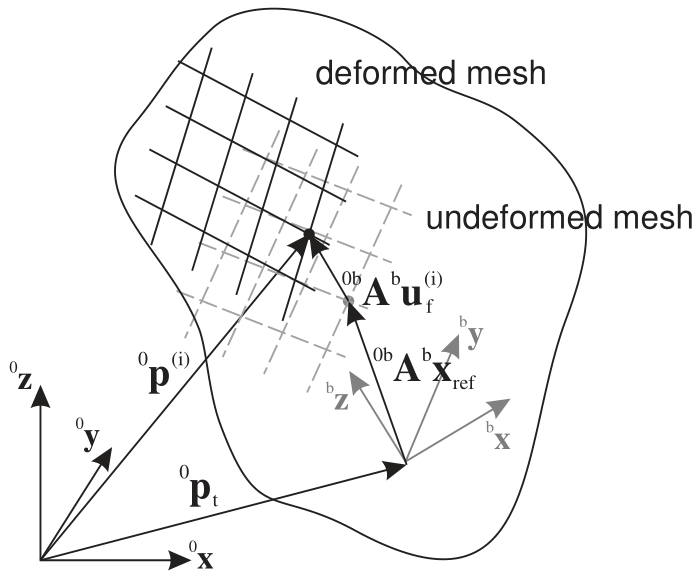
\includegraphics[width=8cm]{figures/ObjectFFRFsketch.pdf}
      \end{center}
      \caption{Floating frame of reference with exemplary position of a mesh node $i$.}
        \label{fig:ObjectFFRFreducedOrder:mesh}
    \end{figure}
    }
    \onlyRST{
    .. _fig-objectffrfreducedorder-mesh:
    .. figure:: docs/theDoc/figures/ObjectFFRFsketch.png
       :width: 400

       Floating frame of reference with exemplary position of a mesh node *i* 
    }
    %++++++++++++++++++++++++

                       
    The reduced order \hac{FFRF} formulation is based on an approximation of flexible coordinates $\LU{b}{\qv\indf}$ 
    by means of a reduction or mode basis $\LU{b}{\tPsi}$ (\texttt{modeBasis}) and the the modal coordinates $\tzeta$,
    \be
      \LU{b}{\qv\indf} \approx \LU{b}{\tPsi} \tzeta
    \ee
    The mode basis $\LU{b}{\tPsi}$ contains so-called mode shape vectors in its columns, which may be computed from eigen analysis, static computation or more advanced techniques, 
    see the helper functions in module \texttt{exudyn.FEM}, within the class \text{FEMinterface}.
    To compute eigen modes, use \texttt{FEMinterface.ComputeEigenmodes(...)} or
    \texttt{FEMinterface.ComputeHurtyCraigBamptonModes(...)}. For details on model order reduction and component mode synthesis, see \refSection{sec:theory:CMS}.
    In many applications, $n_m$ typically ranges between 10 and 50, but also beyond -- depending on the desired accuracy of the model.
    
    The \texttt{ObjectFFRF} coordinates and \eqs{eq:ObjectFFRF:eom}\footnote{this is not done for user functions and \texttt{forceVector}} can be reduced by the matrix $\Hm \in \Rcal^{(n\indf+n\indrigid) \times n_{ODE2}}$,
    \be
      \qv_{FFRF} = \vr{\qv\indt}{\ttheta}{\LU{b}{\qv\indf}} = \mr{\ImThree}{\Null}{\Null} {\Null}{\Im\indr}{\Null} {\Null}{\Null}{\LU{b}{\tPsi}} \vr{\qv\indt}{\ttheta}{\tzeta}
        = \Hm \, \qv
    \ee
    with the $4\times 4$ identity matrix $\Im\indr$ in case of Euler parameters and the reduced coordinates $\qv$.
    
    The reduced equations follow from the reduction of system matrices in \eqs{eq:ObjectFFRF:eom},
    \bea
      \Km\indred &=& \LU{b}{\tPsi}\tp \LU{b}{\Km} \LU{b}{\tPsi} \eqComma \\
      \Mm\indred &=& \LU{b}{\tPsi}\tp \LU{b}{\Mm} \LU{b}{\tPsi} \eqComma \\
    \eea
    the computation of rigid body inertia
    \bea
      \LU{b}{\tTheta}\indu &=& \LUX{b}{\tilde \xv}{\cRef\tp} \LU{b}{\Mm} \LU{b}{\tilde \xv\cRef}\\
    \eea
    the center of mass (and according tilde matrix), using $\tPhi\indt$ from \eq{eq:ObjectFFRF:Phit},
    \bea
      \LU{b}{\tchi}\indu &=& \frac{1}{m} \tPhi\tp\indt \LU{b}{\Mm} \LU{b}{\xv\cRef}\\
      \LU{b}{\tilde \tchi\indu} &=& \frac{1}{m} \tPhi\tp\indt \LU{b}{\Mm} \LU{b}{\tilde \xv\cRef}\\
    \eea 
    and seven inertia-like matrices \cite{ZwoelferGerstmayr2021},
    \be
      \Mm_{AB} = \Am\tp \LU{b}{\Mm} \Bm, \quad \mathrm{using} \quad \Am\Bm \in \left[\tPsi\tPsi ,\; \widetilde{\tPsi}\tPsi,\; \widetilde{\tPsi}\widetilde{\tPsi},\; 
        \tPhi\indt\tPsi,\; \tPhi\indt\widetilde{\tPsi},\; \tilde\xv\cRef\tPsi,\; \tilde\xv\cRef\widetilde{\tPsi}\right]
    \ee
    Note that the special tilde operator for vectors $\pv \in \Rcal^{n_f}$ of \eq{eq:ObjectFFRF:specialTilde} is frequently used.
    
    
    %+++++++++++++++++++++++++
    %+++++++++++++++++++++++++
    %+++++++++++++++++++++++++
    %+++++++++++++++++++++++++
    \mysubsubsubsection{Equations of motion}
    Equations of motion, in case that \texttt{computeFFRFterms = True}:
    \bea
        \left(\Mm_{user}(mbs, t,\qv,\dot \qv) + 
                    \mr{\Mm\indtt}{\Mm\indtr}{\Mm\indtf} {}{\Mm\indrr}{\Mm\indrf} {\mathrm{sym.}}{}{\Mm\indff} \right) \ddot \qv + 
                    \mr{0}{0}{0} {0}{0}{0} {0}{0}{\Dm\indff} \dot \qv + \mr{0}{0}{0} {0}{0}{0} {0}{0}{\Km\indff} \qv = &&\\ \nonumber
                    \fv_v(\qv,\dot \qv) + \fv_{user}(mbs, t,\qv,\dot \qv) &&
    \eea
    \footnote{NOTE that currently the internal (C++) computed terms are zero,
    \be
      \mr{\Mm\indtt}{\Mm\indtr}{\Mm\indtf} {}{\Mm\indrr}{\Mm\indrf} {\mathrm{sym.}}{}{\Mm\indff} = \Null \quad \mathrm{and} \quad
        \fv_v(\qv,\dot \qv) = \Null \eqComma
    \ee
    but they are implemented in predefined user functions, see \texttt{FEM.py}, \refSection{sec:FEM:ObjectFFRFreducedOrderInterface:AddObjectFFRFreducedOrderWithUserFunctions}. In near future, these terms will be implemented in C++ and replace the user functions.}
    %
    Note that in case of Euler parameters for the parameterization of rotations for the reference frame, the Euler parameter constraint equation is added automatically by this object.
    %
    The single terms of the mass matrix are defined as\cite{ZwoelferGerstmayr2021}
    \bea
      \Mm\indtt &=& m \ImThree \\
      \Mm\indtr &=& -\LU{0b}{\Rot} \left[ m \LU{b}{\tilde \tchi\indu} + \Mm_{\Phi\indt\!{\widetilde\Psi}} 
                      \left( \tzeta \otimes \Im \right)  \right] \LU{b}{\Gm}\\
      \Mm\indtf &=& \LU{0b}{\Rot} \Mm_{\Phi\indt\!\Psi} \\
      \Mm\indrr &=& \LU{b}{\Gm\tp} \left[\LU{b}{\tTheta}\indu + 
                                          \Mm_{\tilde \xv\cRef{\widetilde\Psi}} \left( \tzeta \otimes \Im \right) +
                                                                            \left( \tzeta \otimes \Im \right)\tp \Mm_{\tilde \xv\cRef{\widetilde\Psi}}\tp +
                                                                            \left( \tzeta \otimes \Im \right)\tp \Mm_{{\widetilde\Psi}{\widetilde\Psi}}\left( \tzeta \otimes \Im \right)
                                                                            \right] \LU{b}{\Gm}\\
      \Mm\indrf &=& -\LU{b}{\Gm\tp} \left[ \Mm_{\tilde \xv\cRef\Psi} + \left( \tzeta \otimes \Im \right)\tp \Mm_{{\widetilde\Psi}\Psi}  \right] \\ 
      \Mm\indff &=& \Mm_{\Psi\Psi}
    \eea
    with the Kronecker product\footnote{In Python numpy module this is computed by \texttt{numpy.kron(zeta, Im).T}},
    \be
      \tzeta \otimes \Im = \vr{\zeta_0 \Im}{\vdots}{\zeta_{m-1} \Im}
    \ee
    The quadratic velocity vector $\fv_v(\qv,\dot \qv) = \left[ \fv_{v\mathrm{t}}\tp,\; \fv_{v\mathrm{r}}\tp,\; \fv_{v\mathrm{f}}\tp \right]\tp$ reads
    \bea
      \fv_{v\mathrm{t}} &=& \LU{0b}{\Rot} \LU{b}{\tilde \tomega}\left[ m \LU{b}{\tilde \tchi\indu} + \Mm_{\Phi\indt\!{\widetilde\Psi}} 
                      \left( \tzeta \otimes \Im \right)  \right] \LU{b}{\tomega} + 
                                    2 \LU{0b}{\Rot} \Mm_{\Phi\indt\!{\widetilde\Psi}} \left( \dot \tzeta \otimes \Im \right)  \LU{b}{\tomega} \nonumber \\
                                && + \LU{0b}{\Rot} \left[ m \LU{b}{\tilde \tchi\indu} + \Mm_{\Phi\indt\!{\widetilde\Psi}} 
                      \left( \tzeta \otimes \Im \right)  \right] \LU{b}{\dot \Gm} \dot \ttheta \eqComma \\
        \fv_{v\mathrm{r}} &=& -\LU{b}{\Gm\tp} \LU{b}{\tilde \tomega} \left[\LU{b}{\tTheta}\indu + 
                                          \Mm_{\tilde \xv\cRef{\widetilde\Psi}} \left( \tzeta \otimes \Im \right) +
                                                                            \left( \tzeta \otimes \Im \right)\tp \Mm_{\tilde \xv\cRef{\widetilde\Psi}}\tp +
                                                                            \left( \tzeta \otimes \Im \right)\tp \Mm_{{\widetilde\Psi}{\widetilde\Psi}}\left( \tzeta \otimes \Im \right)
                                                                            \right]\LU{b}{\tomega} \nonumber \\
                                            && -2 \LU{b}{\Gm\tp} \left[ \Mm_{\tilde \xv\cRef{\widetilde\Psi}} \left( \dot \tzeta \otimes \Im \right) +
                                                                                        \left( \tzeta \otimes \Im \right)\tp \Mm_{{\widetilde\Psi}{\widetilde\Psi}}\left( \dot \tzeta \otimes \Im \right)
                                                                 \right] \LU{b}{\tomega} \nonumber \\
                                            && -\LU{b}{\Gm\tp}\left[\LU{b}{\tTheta}\indu + 
                                          \Mm_{\tilde \xv\cRef{\widetilde\Psi}} \left( \tzeta \otimes \Im \right) +
                                                                            \left( \tzeta \otimes \Im \right)\tp \Mm_{\tilde \xv\cRef{\widetilde\Psi}}\tp +
                                                                            \left( \tzeta \otimes \Im \right)\tp \Mm_{{\widetilde\Psi}{\widetilde\Psi}}\left( \tzeta \otimes \Im \right)
                                                                            \right] \LU{b}{\dot \Gm} \dot \ttheta \eqComma \\
        \fv_{v\mathrm{f}} &=& \left( \Im_\zeta \otimes \LU{b}{\tomega} \right)\tp 
                                    \left[ \Mm_{\tilde\xv\cRef{\widetilde\Psi}}\tp + \Mm_{{\widetilde\Psi}{\widetilde\Psi}}\left( \tzeta \otimes \Im \right) \right] \LU{b}{\tomega}
                                                                +2 \Mm_{{\widetilde\Psi}{\Psi}}\tp\left( \dot\tzeta \otimes \Im \right) \LU{b}{\tomega} \nonumber \\
                                            && + \left[ \Mm_{\tilde\xv\cRef{\Psi}}\tp + \Mm_{{\widetilde\Psi}{\Psi}}\tp\left( \tzeta \otimes \Im \right)
                                                 \right] \LU{b}{\dot \Gm} \dot \ttheta \eqDot
    \eea
    Note that terms including $\LU{b}{\dot \Gm} \dot \ttheta$ vanish in case of Euler parameters or in case that $\LU{b}{\dot \Gm} = \Null$,
    and we use another Kronecker product with the unit matrix $\Im_\zeta \in \Rcal^{n_m \times n_m}$,
    \be
      \Im_\zeta \otimes \LU{b}{\tomega} = \mr{\LU{b}{\tomega}}{}{} {}{\ddots}{} {}{}{\LU{b}{\tomega}} \in \Rcal^{3n_m \times n_m}
    \ee
    
    %$\ra$ will be completed later, see according literature of Zw{\"o}lfer and Gerstmayr \cite{ZwoelferGerstmayr2021}.
    
    In case that \texttt{computeFFRFterms = False}, the mass terms $\Mm\indtt \ldots \Mm\indff$ are zero (not computed) and
    the quadratic velocity vector $\fv_Q = \Null$.
    Note that the user functions $\fv_{user}(mbs, t,\qv,\dot \qv)$ and 
    $\Mm_{user}(mbs, t,\qv,\dot \qv)$ may be empty (=0). 
    The detailed equations of motion for this element can be found in \cite{ZwoelferGerstmayr2021}.

    %+++++++++++++++++++++++++
    %+++++++++++++++++++++++++
    \mysubsubsubsection{Position Jacobian}
    For joints and loads, the position jacobian of a node is needed in order to compute forces applied to averaged displacements and 
    rotations at nodes.
    Recall that the modal coordinates $\tzeta$ are transformed to node coordinates by means of the mode basis  $\LU{b}{\tPsi}$,
    \be
      \LU{b}{\qv\indf} = \LU{b}{\tPsi} \tzeta \eqDot
    \ee
    The local displacements $\LU{b}{\uv\indf^{(i)}}$ of a specific node $i$ can be reconstructed in this way by means of
    \be
      \LU{b}{\uv\indf^{(i)}} = \vr{\LU{b}{\qv_{\mathrm{f},i\cdot 3}}}{\LU{b}{\qv_{\mathrm{f},i\cdot 3+1}}}{\LU{b}{\qv_{\mathrm{f},i\cdot 3+2}}} \eqComma
    \ee
    and the global position of a node, see tables above, reads
    \be
      \LU{0}{\pv^{(i)}} = \LU{0}{\pv\indt} + \LU{0b}{\Am} \left( \LU{b}{\uv\indf^{(i)}} + \LU{b}{\xv^{(i)}\cRef} \right)
    \ee
    Thus, the jacobian of the global position reads
    \be
     \LU{0}{\Jm_\mathrm{pos}^{(i)}} = \frac{\partial \LU{0}{\pv^{(i)}}}{\partial [\qv\indt, \;\ttheta, \;\tzeta]}
     = \left[\ImThree, \; -\LU{0b}{\Rot} \left(\LU{b}{\tilde\uv\indf^{(i)}} + \LU{b}{\tilde\xv^{(i)}\cRef} \right) \LU{b}{\Gm},\;
             \LU{0b}{\Rot} \vr{\LU{b}{\tPsi_{r=3i}\tp}}{\LU{b}{\tPsi_{r=3i+1}\tp}}{\LU{b}{\tPsi_{r=3i+2}\tp}}\right] \eqComma
    \ee
    in which $\LU{b}{\tPsi_{r=...}}$ represents the row $r$ of the mode basis (matrix) $\LU{b}{\Psi}$, and
    the matrix 
    \be
      \vr{\LU{b}{\tPsi_{r=3i}\tp}}{\LU{b}{\tPsi_{r=3i+1}\tp}}{\LU{b}{\tPsi_{r=3i+2}\tp}} \in \Rcal^{3 \times n_m}
    \ee
    Furthermore, the jacobian of the local position reads
    \be
     \LU{b}{\Jm_\mathrm{pos}^{(i)}} = \frac{\partial \LU{b}{\pv\indf^{(i)}}}{\partial [\qv\indt, \;\ttheta, \;\tzeta]}
     = \left[\Null, \; \Null, \; \vr{\LU{b}{\tPsi_{r=3i}\tp}}{\LU{b}{\tPsi_{r=3i+1}\tp}}{\LU{b}{\tPsi_{r=3i+2}\tp}}\right] \eqComma
    \ee
    which is used in \texttt{MarkerSuperElementRigid}.
    
    
    %+++++++++++++++++++++++++
    %+++++++++++++++++++++++++
    \mysubsubsubsection{Joints and Loads}
    Use special \texttt{MarkerSuperElementPosition} to apply forces, SpringDampers or spherical joints. This marker can be attached to a single node of the underlying
    mesh or to a set of nodes, which is then averaged, see the according marker description.
    
    Use special \texttt{MarkerSuperElementRigid} to apply torques or special joints (e.g., \texttt{JointGeneric}). 
    This marker must be attached to a set of nodes which can represent rigid body motion. The rigid body motion is then averaged for all of these nodes,
    see the according marker description.
    
    For application of mass proportional loads (gravity), you can use conventional MarkerBodyMass.
    However, {\bf do not use} \texttt{MarkerBodyPosition} or \texttt{MarkerBodyRigid} for ObjectFFRFreducedOrder, unless wanted, because it only attaches to the floating
    frame. This means, that a force to a \texttt{MarkerBodyPosition} would only be applied to the (rigid) floating frame, but not onto the deformable body and
    results depend strongly on the choice of the reference frame (or the underlying mode shapes).
    
    CoordinateLoads are added for each \hac{ODE2} coordinate on the RHS of the equations of motion. 
    %++++++++++++++++++++++++++++++++++++++++
    
    
    %++++++++++++++++++++++++++++++++++++++++++++++++++++++++++
    \userFunction{forceUserFunction(mbs, t, itemNumber, q, q\_t)}
    A user function, which computes a force vector depending on current time and states of object. Can be used to create any kind of mechanical system by using the object states.
    Note that itemNumber represents the index of the ObjectFFRFreducedOrder object in mbs, which can be used to retrieve additional data from the object through
    \texttt{mbs.GetObjectParameter(itemNumber, ...)}, see the according description of \texttt{GetObjectParameter}.
    %
    \startTable{arguments /  return}{type or size}{description}
      \rowTable{\texttt{mbs}}{MainSystem}{provides MainSystem mbs to which object belongs}
      \rowTable{\texttt{t}}{Real}{current time in mbs}
      \rowTable{\texttt{itemNumber}}{Index}{integer number of the object in mbs, allowing easy access to all object data via mbs.GetObjectParameter(itemNumber, ...)}
      \rowTable{\texttt{q}}{Vector $\in \Rcal^n_{ODE2}$}{\hac{FFRF} object coordinates (rigid body coordinates and reduced coordinates in a list) in current configuration, without reference values}
      \rowTable{\texttt{q\_t}}{Vector $\in \Rcal^n_{ODE2}$}{object velocity coordinates (time derivatives of \texttt{q}) in current configuration}
      \rowTable{\returnValue}{Vector $\in \Rcal^{n_{ODE2}}$}{returns force vector for object}
    \finishTable
    %++++++++++++++++++++++++++++++++++++++++++++++++++++++++++
    \userFunction{massMatrixUserFunction(mbs, t, itemNumber, q, q\_t)}
    A user function, which computes a mass matrix depending on current time and states of object. Can be used to create any kind of mechanical system by using the object states.
    \startTable{arguments /  return}{type or size}{description}
      \rowTable{\texttt{mbs}}{MainSystem}{provides MainSystem mbs to which object belongs}
      \rowTable{\texttt{t}}{Real}{current time in mbs}
      \rowTable{\texttt{itemNumber}}{Index}{integer number of the object in mbs, allowing easy access to all object data via mbs.GetObjectParameter(itemNumber, ...)}
      \rowTable{\texttt{q}}{Vector $\in \Rcal^n_{ODE2}$}{\hac{FFRF} object coordinates (rigid body coordinates and reduced coordinates in a list) in current configuration, without reference values}
      \rowTable{\texttt{q\_t}}{Vector $\in \Rcal^n_{ODE2}$}{object velocity coordinates (time derivatives of \texttt{q}) in current configuration}
      \rowTable{\returnValue}{NumpyMatrix $\in \Rcal^{n_{ODE2} \times n_{ODE2}}$}{returns mass matrix for object}
    \finishTable
    \vspace{12pt}
    %++++++++++++++++++++++++++++++++++++++++++++++++++++++++++
    %%RSTCOMPATIBLE
\vspace{6pt}\par\noindent\rule{\textwidth}{0.4pt}
%
\noindent For examples on ObjectFFRFreducedOrder see Relevant Examples and TestModels with weblink:
\bi
\item \exuUrl{https://github.com/jgerstmayr/EXUDYN/blob/master/main/pythonDev/Examples/NGsolvePistonEngine.py}{\texttt{NGsolvePistonEngine.py}} (Examples/)
\item \exuUrl{https://github.com/jgerstmayr/EXUDYN/blob/master/main/pythonDev/Examples/objectFFRFreducedOrderNetgen.py}{\texttt{objectFFRFreducedOrderNetgen.py}} (Examples/)
\item \exuUrl{https://github.com/jgerstmayr/EXUDYN/blob/master/main/pythonDev/TestModels/NGsolveCrankShaftTest.py}{\texttt{NGsolveCrankShaftTest.py}} (TestModels/)
\item \exuUrl{https://github.com/jgerstmayr/EXUDYN/blob/master/main/pythonDev/TestModels/objectFFRFreducedOrderAccelerations.py}{\texttt{objectFFRFreducedOrderAccelerations.py}} (TestModels/)
\item \exuUrl{https://github.com/jgerstmayr/EXUDYN/blob/master/main/pythonDev/TestModels/objectFFRFreducedOrderShowModes.py}{\texttt{objectFFRFreducedOrderShowModes.py}} (TestModels/)
\item \exuUrl{https://github.com/jgerstmayr/EXUDYN/blob/master/main/pythonDev/TestModels/objectFFRFreducedOrderStressModesTest.py}{\texttt{objectFFRFreducedOrderStressModesTest.py}} (TestModels/)
\item \exuUrl{https://github.com/jgerstmayr/EXUDYN/blob/master/main/pythonDev/TestModels/superElementRigidJointTest.py}{\texttt{superElementRigidJointTest.py}} (TestModels/)

\ei

%

\newpage
%+++++++++++++++++++++++++++++++
%+++++++++++++++++++++++++++++++
\mysubsection{Objects (FiniteElement)}
A FiniteElement is a special Object and Body, which is used to define deformable bodies, such as beams or solid finite elements. FiniteElements are usually linked to two or more nodes.
%++++++

%+++++++++++++++++++++++++++++++++++

\mysubsubsection{ObjectANCFCable}
\label{sec:item:ObjectANCFCable}
A 3D cable finite element using 2 nodes of type NodePointSlope1. The localPosition of the beam with length $L$=physicsLength and height $h$ ranges in $X$-direction in range $[0, L]$ and in $Y$-direction in range $[-h/2,h/2]$ (which is in fact not needed in the \hac{EOM}). For description see ObjectANCFCable2D, which is almost identical to 3D case. Note that this element does not include torsion, therfore a torque cannot be applied along the local x-axis.
\vspace{12pt}\\

\noindent \mybold{Additional information for ObjectANCFCable}:
\bi
  \item This \texttt{Object} has/provides the following types = \texttt{Body}, \texttt{MultiNoded}
  \item Requested \texttt{Node} type = \texttt{Position}
  \item {\bf Short name} for Python = \texttt{Cable}
  \item {\bf Short name} for Python visualization object = \texttt{VCable}
\ei\vspace{12pt} \noindent 
The item \mybold{ObjectANCFCable} with type = 'ANCFCable' has the following parameters:
\vspace{-0.5cm}\\
\vspace{-0.5cm}\\
%reference manual TABLE
\begin{center}
  \footnotesize
  \begin{longtable}{| p{4.5cm} | p{2.5cm} | p{0.5cm} | p{2.5cm} | p{6cm} |}
    \hline
    \bf Name & \bf type & \bf size & \bf default value & \bf description \\ \hline
    name &     String &      &     '' &     objects's unique name\\ \hline
    physicsLength &     UReal &      &     0. &      [SI:m] reference length of beam; such that the total volume (e.g. for volume load) gives $\rho A L$; must be positive\\ \hline
    physicsMassPerLength &     UReal &      &     0. &      [SI:kg/m] mass per length of beam\\ \hline
    physicsBendingStiffness &     UReal &      &     0. &      [SI:Nm$^2$] bending stiffness of beam; the bending moment is $m = EI (\kappa - \kappa_0)$, in which $\kappa$ is the material measure of curvature\\ \hline
    physicsAxialStiffness &     UReal &      &     0. &      [SI:N] axial stiffness of beam; the axial force is $f_{ax} = EA (\varepsilon -\varepsilon_0)$, in which $\varepsilon = |\rv^\prime|-1$ is the axial strain\\ \hline
    physicsBendingDamping &     UReal &      &     0. &      [SI:Nm$^2$/s] bending damping of beam ; the additional virtual work due to damping is $\delta W_{\dot \kappa} = \int_0^L \dot \kappa \delta \kappa dx$\\ \hline
    physicsAxialDamping &     UReal &      &     0. &      [SI:N/s] axial damping of beam; the additional virtual work due to damping is $\delta W_{\dot\varepsilon} = \int_0^L \dot \varepsilon \delta \varepsilon dx$\\ \hline
    physicsReferenceAxialStrain &     Real &      &     0. &      [SI:1] reference axial strain of beam (pre-deformation) of beam; without external loading the beam will statically keep the reference axial strain value\\ \hline
    strainIsRelativeToReference &     Real &      &     0. &      if set to 1., a pre-deformed reference configuration is considered as the stressless state; if set to 0., the straight configuration plus the values of $\varepsilon_0$ and $\kappa_0$ serve as a reference geometry; allows also values between 0. and 1.\\ \hline
    nodeNumbers &     NodeIndex2 &      &     [invalid [-1], invalid [-1]] &     \tabnewline two node numbers ANCF cable element\\ \hline
    useReducedOrderIntegration &     Index &      &     0 &     0/false: use Gauss order 9 integration for virtual work of axial forces, order 5 for virtual work of bending moments; 1/true: use Gauss order 7 integration for virtual work of axial forces, order 3 for virtual work of bending moments\\ \hline
    visualization &     VObjectANCFCable &      &      &     parameters for visualization of item\\ \hline
\end{longtable}
\end{center}

\noindent The item VObjectANCFCable has the following parameters:
%reference manual TABLE
\begin{center}
  \footnotesize
  \begin{longtable}{| p{4.5cm} | p{2.5cm} | p{0.5cm} | p{2.5cm} | p{6cm} |}
    \hline
    \bf Name & \bf type & \bf size & \bf default value & \bf description \\ \hline
    show &     Bool &      &     True &     set true, if item is shown in visualization and false if it is not shown; note that all quantities are computed at the beam centerline, even if drawn on surface of cylinder of beam; this effects, e.g., Displacement or Velocity, which is drawn constant over cross section\\ \hline
    radius &     float &      &     0. &     if radius==0, only the centerline is drawn; else, a cylinder with radius is drawn; circumferential tiling follows general.cylinderTiling and beam axis tiling follows bodies.beams.axialTiling\\ \hline
    color &     Float4 &      &     [-1.,-1.,-1.,-1.] &     \tabnewline RGBA color of the object; if R==-1, use default color\\ \hline
\end{longtable}
\end{center}
\par\noindent\rule{\textwidth}{0.4pt}
\mysubsubsubsection{DESCRIPTION of ObjectANCFCable:}
\label{description_ObjectANCFCable}
\paragraph{Information on input parameters:} 
\startTable{input parameter}{symbol}{description see tables above}
\rowTable{physicsLength}{$L$}{}
\rowTable{physicsMassPerLength}{$\rho A$}{}
\rowTable{physicsBendingStiffness}{$EI$}{}
\rowTable{physicsAxialStiffness}{$EA$}{}
\rowTable{physicsBendingDamping}{$d_{K}$}{}
\rowTable{physicsAxialDamping}{$d_{\varepsilon}$}{}
\rowTable{physicsReferenceAxialStrain}{$\varepsilon_0$}{}
\rowTable{strainIsRelativeToReference}{$f\cRef$}{}
\finishTable

\mybold{The following output variables are available as OutputVariableType in sensors, Get...Output() and other functions}:
\begin{center}
\footnotesize
\begin{longtable}{| p{5cm} | p{5cm} | p{6cm} |} 
\hline
\bf output variable & \bf symbol & \bf description \\ \hline
Position & $\LU{0}{\pv\cConfig(x,0,0)} = \rv\cConfig(x) + y\cdot \nv\cConfig(x)$ & global position vector of local position $[x,0,0]$\\ \hline
Displacement & $\LU{0}{\uv\cConfig(x,0,0)} = \LU{0}{\pv\cConfig(x,0,0)} - \LU{0}{\pv\cRef(x,0,0)}$ & global displacement vector of local position\\ \hline
Velocity & $\LU{0}{\vv(x,0,0)} = \LU{0}{\dot \rv(x)}$ & global velocity vector of local position\\ \hline
Director1 & $\rv'(x)$ & (axial) slope vector of local axis position (at $y$=0)\\ \hline
StrainLocal & $\varepsilon$ & axial strain (scalar) of local axis position (at Y=Z=0)\\ \hline
CurvatureLocal & $[K_x, K_y, K_z]\tp$ & local curvature vector\\ \hline
ForceLocal & $N$ &  (local) section normal force (scalar, including reference strains) (at $y$=$z$=0); note that strains are highly inaccurate when coupled to bending, thus consider useReducedOrderIntegration=2 and evaluate axial strain at nodes or at midpoint\\ \hline
TorqueLocal & $M$ &  (local) bending moment (scalar) (at $y$=$z$=0), which are bending moments as there is no torque\\ \hline
Acceleration & $\LU{0}{\av(x,0,0)} = \LU{0}{\ddot \rv(x)}$ & global acceleration vector of local position\\ \hline
\end{longtable}
\end{center}
 \noindent
    %%RSTCOMPATIBLE
\vspace{6pt}\par\noindent\rule{\textwidth}{0.4pt}
\mysubsubsubsection{MINI EXAMPLE for ObjectANCFCable}
\label{miniExample_ObjectANCFCable}
\pythonstyle
\begin{lstlisting}[language=Python, firstnumber=1]
    from exudyn.beams import GenerateStraightLineANCFCable
    rhoA = 78.
    EA = 1000000.
    EI = 833.3333333333333
    cable = Cable(physicsMassPerLength=rhoA, 
                  physicsBendingStiffness=EI, 
                  physicsAxialStiffness=EA, 
                  )

    ancf=GenerateStraightLineANCFCable(mbs=mbs,
                  positionOfNode0=[0,0,0], positionOfNode1=[2,0,0],
                  numberOfElements=32, #converged to 4 digits
                  cableTemplate=cable, #this defines the beam element properties
                  massProportionalLoad = [0,-9.81,0],
                  fixedConstraintsNode0 = [1,1,1, 0,1,1], #add constraints for pos and rot (r'_y,r'_z)
                  )
    lastNode = ancf[0][-1]

    #assemble and solve system for default parameters
    mbs.Assemble()
    mbs.SolveStatic()

    #check result
    exudynTestGlobals.testResult = mbs.GetNodeOutput(lastNode, exu.OutputVariableType.Displacement)[0]
    #ux=-0.5013058140308901
\end{lstlisting}

\newpage

%+++++++++++++++++++++++++++++++++++

\mysubsubsection{ObjectANCFCable2D}
\label{sec:item:ObjectANCFCable2D}
A 2D cable finite element using 2 nodes of type NodePoint2DSlope1. The localPosition of the beam with length $L$=physicsLength and height $h$ ranges in $X$-direction in range $[0, L]$ and in $Y$-direction in range $[-h/2,h/2]$ (which is in fact not needed in the \hac{EOM}).
\vspace{12pt}\\

\noindent \mybold{Additional information for ObjectANCFCable2D}:
\bi
  \item Requested \texttt{Node} type = \texttt{Position2D} + \texttt{Orientation2D} + \texttt{Point2DSlope1} + \texttt{Position} + \texttt{Orientation}
  \item {\bf Short name} for Python = \texttt{Cable2D}
  \item {\bf Short name} for Python visualization object = \texttt{VCable2D}
\ei\vspace{12pt} \noindent 
The item \mybold{ObjectANCFCable2D} with type = 'ANCFCable2D' has the following parameters:
\vspace{-0.5cm}\\
\vspace{-0.5cm}\\
%reference manual TABLE
\begin{center}
  \footnotesize
  \begin{longtable}{| p{4.5cm} | p{2.5cm} | p{0.5cm} | p{2.5cm} | p{6cm} |}
    \hline
    \bf Name & \bf type & \bf size & \bf default value & \bf description \\ \hline
    name &     String &      &     '' &     objects's unique name\\ \hline
    physicsLength &     UReal &      &     0. &      [SI:m] reference length of beam; such that the total volume (e.g. for volume load) gives $\rho A L$; must be positive\\ \hline
    physicsMassPerLength &     UReal &      &     0. &      [SI:kg/m] mass per length of beam\\ \hline
    physicsBendingStiffness &     UReal &      &     0. &      [SI:Nm$^2$] bending stiffness of beam; the bending moment is $m = EI (\kappa - \kappa_0)$, in which $\kappa$ is the material measure of curvature\\ \hline
    physicsAxialStiffness &     UReal &      &     0. &      [SI:N] axial stiffness of beam; the axial force is $f_{ax} = EA (\varepsilon -\varepsilon_0)$, in which $\varepsilon = |\rv^\prime|-1$ is the axial strain\\ \hline
    physicsBendingDamping &     UReal &      &     0. &      [SI:Nm$^2$/s] bending damping of beam ; the additional virtual work due to damping is $\delta W_{\dot \kappa} = \int_0^L \dot \kappa \delta \kappa dx$\\ \hline
    physicsAxialDamping &     UReal &      &     0. &      [SI:N/s] axial damping of beam; the additional virtual work due to damping is $\delta W_{\dot\varepsilon} = \int_0^L \dot \varepsilon \delta \varepsilon dx$\\ \hline
    physicsReferenceAxialStrain &     Real &      &     0. &      [SI:1] reference axial strain of beam (pre-deformation) of beam; without external loading the beam will statically keep the reference axial strain value\\ \hline
    physicsReferenceCurvature &     Real &      &     0. &      [SI:1/m] reference curvature of beam (pre-deformation) of beam; without external loading the beam will statically keep the reference curvature value\\ \hline
    strainIsRelativeToReference &     Real &      &     0. &      if set to 1., a pre-deformed reference configuration is considered as the stressless state; if set to 0., the straight configuration plus the values of $\varepsilon_0$ and $\kappa_0$ serve as a reference geometry; allows also values between 0. and 1.\\ \hline
    nodeNumbers &     NodeIndex2 &      &     [invalid [-1], invalid [-1]] &     \tabnewline two node numbers ANCF cable element\\ \hline
    useReducedOrderIntegration &     Index &      &     0 &     0/false: use Gauss order 9 integration for virtual work of axial forces, order 5 for virtual work of bending moments; 1/True: use Gauss order 7 integration for virtual work of axial forces, order 3 for virtual work of bending moments; 2: use mixed Lobatto/Gauss integration with exceptional quality of axial strain, however, spurious (hourglass) modes may occur!\\ \hline
    axialForceUserFunction &     PyFunctionMbsScalarIndexScalar9 &     \tabnewline  &     \tabnewline 0 &     A Python function which defines the (nonlinear relations) of local strains (including axial strain and bending strain) as well as time derivatives to the local axial force; see description below\\ \hline
    bendingMomentUserFunction &     PyFunctionMbsScalarIndexScalar9 &     \tabnewline  &     \tabnewline 0 &     A Python function which defines the (nonlinear relations) of local strains (including axial strain and bending strain) as well as time derivatives to the local bending moment; see description below\\ \hline
    visualization &     VObjectANCFCable2D &      &      &     parameters for visualization of item\\ \hline
\end{longtable}
\end{center}

\noindent The item VObjectANCFCable2D has the following parameters:
%reference manual TABLE
\begin{center}
  \footnotesize
  \begin{longtable}{| p{4.5cm} | p{2.5cm} | p{0.5cm} | p{2.5cm} | p{6cm} |}
    \hline
    \bf Name & \bf type & \bf size & \bf default value & \bf description \\ \hline
    show &     Bool &      &     True &     set true, if item is shown in visualization and false if it is not shown\\ \hline
    drawHeight &     float &      &     0. &     if beam is drawn with rectangular shape, this is the drawing height\\ \hline
    color &     Float4 &      &     [-1.,-1.,-1.,-1.] &     \tabnewline RGBA color of the object; if R==-1, use default color\\ \hline
\end{longtable}
\end{center}
\par\noindent\rule{\textwidth}{0.4pt}
\mysubsubsubsection{DESCRIPTION of ObjectANCFCable2D:}
\label{description_ObjectANCFCable2D}
\paragraph{Information on input parameters:} 
\startTable{input parameter}{symbol}{description see tables above}
\rowTable{physicsLength}{$L$}{}
\rowTable{physicsMassPerLength}{$\rho A$}{}
\rowTable{physicsBendingStiffness}{$EI$}{}
\rowTable{physicsAxialStiffness}{$EA$}{}
\rowTable{physicsBendingDamping}{$d_{K}$}{}
\rowTable{physicsAxialDamping}{$d_{\varepsilon}$}{}
\rowTable{physicsReferenceAxialStrain}{$\varepsilon_0$}{}
\rowTable{physicsReferenceCurvature}{$\kappa_0$}{}
\rowTable{strainIsRelativeToReference}{$f\cRef$}{}
\rowTable{axialForceUserFunction}{$\mathrm{UF} \in \Rcal$}{}
\rowTable{bendingMomentUserFunction}{$\mathrm{UF} \in \Rcal$}{}
\finishTable

\mybold{The following output variables are available as OutputVariableType in sensors, Get...Output() and other functions}:
\begin{center}
\footnotesize
\begin{longtable}{| p{5cm} | p{5cm} | p{6cm} |} 
\hline
\bf output variable & \bf symbol & \bf description \\ \hline
Position & $\LU{0}{\pv\cConfig(x,y,0)} = \rv\cConfig(x) + y\cdot \nv\cConfig(x)$ & global position vector of local position $[x,y,0]$\\ \hline
Displacement & $\LU{0}{\uv\cConfig(x,y,0)} = \LU{0}{\pv\cConfig(x,y,0)} - \LU{0}{\pv\cRef(x,y,0)}$ & global displacement vector of local position\\ \hline
Velocity & $\LU{0}{\vv(x,y,0)} = \LU{0}{\dot \rv(x)} - y \cdot \omega_2 \cdot\LU{0}{\tv(x)} $ & global velocity vector of local position\\ \hline
VelocityLocal & $\LU{b}{\vv(x,y,0)} = \LU{b0}{\Rot}\LU{0}{\vv(x,y,0)}$ & local velocity vector of local position\\ \hline
Rotation & $\varphi = \mathrm{atan2}(r'_y, r'_x)$ & (scalar) rotation angle of axial slope vector (relative to global $x$-axis)\\ \hline
Director1 & $\rv'(x)$ & (axial) slope vector of local axis position (at $y$=0)\\ \hline
StrainLocal & $\varepsilon$ & axial strain (scalar) of local axis position (at Y=0)\\ \hline
CurvatureLocal & $K$ & axial strain (scalar)\\ \hline
ForceLocal & $N$ &  (local) section normal force (scalar, including reference strains) (at $y$=0); note that strains are highly inaccurate when coupled to bending, thus consider useReducedOrderIntegration=2 and evaluate axial strain at nodes or at midpoint\\ \hline
TorqueLocal & $M$ &  (local) bending moment (scalar) (at $y$=0)\\ \hline
AngularVelocity & $\tomega = [0,\, ,0,\, \omega_2]$ & angular velocity of local axis position (at $y$=0)\\ \hline
Acceleration & $\LU{0}{\av(x,y,0)} = \LU{0}{\ddot \rv(x)} - y \cdot \dot\omega_2 \cdot\LU{0}{\tv(x)}- y \cdot \omega_2 \cdot\LU{0}{\dot\tv(x)} $ & global acceleration vector of local position\\ \hline
AngularAcceleration & $\talpha = [0,\, ,0,\, \dot\omega_2]$ & angular acceleration of local axis position\\ \hline
\end{longtable}
\end{center}
 \noindent
    \mysubsubsubsection{Definition of quantities}
    \startTable{intermediate variables}{symbol}{description}
      \rowTable{beam height}{$h$}{beam height used in several definitions, but effectively undefined. The geometry of the cross section has no influence except for drawing or contact.}
      \rowTable{local beam position}{$\pLocB=[x,\, y,\, 0]\tp$}{local position at axial coordinate $x \in [0,L]$ and cross section coordinate $y \in [-h/2, h/2]$. }
      \rowTable{beam axis position}{$\LU{0}{\rv(x)} = \rv(x) $}{}
      \rowTable{beam axis slope}{$\LU{0}{\rv'(x)} = \rv'(x) $}{}
      \rowTable{beam axis tangent}{$\LU{0}{\tv(x)} = \frac{\rv'(x)}{\Vert \rv(x)'\Vert} $}{this (normalized) vector is normal to cross section}
      \rowTable{beam axis normal}{$\LU{0}{\nv(x)} = [n_x,\, n_y]\tp = [-t_y,\, t_x]\tp  $}{this (normalized) vector lies within the cross section and defines positive $y$-direction.}
      \rowTable{angular velocity}{$\omega_2 = (-r'_y \cdot \dot r'_x + r'_x \cdot \dot r'_y) / \Vert \rv(x)'\Vert^2 $}{}
      \rowTable{rotation matrix}{$\LU{0b}{\Rot}$}{}
      %\rowTable{}{$\LU{0}{\fv} $}{}
      %\rowTable{}{$\LU{0}{\fv} $}{}
    \finishTable

    The Bernoulli-Euler beam is capable of large axial and bendig deformation as it employs the material measure of curvature for the bending.
    %
    \mysubsubsubsection{Kinematics and interpolation}
    %
    Note that in this section, expressions are written in 2D, while output variables are in general 3D quantities, adding a zero for the $z$-coordinate.
    %
    ANCF elements follow the original concept proposed by Shabana \cite{shabana1997ancf}.
    The present 2D element is based on the interpolation used by Berzeri and Shabana \cite{berzeri2000}, but the formulation (especially of the elastic forces) is according to
    Gerstmayr and Irschik \cite{GerstmayrIrschik2008}.
    Slight improvements for the integration of elastic forces and additional terms for off-axis forces and constraints are mentioned here.
    
    The current position of an arbitrary element at local axial position $x \in [0,L]$, where $L$ is the beam length, reads
    \be
      \rv=\rv(x, t),
    \ee
    The derivative of the position w.r.t.\ the axial reference coordinate is denoted as slope vector,
    \be
      \rv'= \frac{\partial \rv(x, t)}{\partial x}
    \ee
    The interpolation is based on cubic (spline) interpolation of position, displacements and velocities.
    The generalized coordinates $\qv \in \Rcal^8$ of the beam element is defined by
    \be
      \qv= \left[\, \rv_0^{T}\;\;\rv_0^{' T}\;\; \rv_1^{T}\;\; \rv_1^{' T}\, \right]^{T}.
    \ee
    in which $\rv_0$ is the position of node 0 and $\rv_1$ is the position of node 1,
    $\rv'_0$ the slope at node 0 and $\rv'_1$ the slope at node 1.
    Note that ANCF coordinates in the present notation are computed as sum of reference and current coordinates
    \be
      \qv = \qv\cCur + \qv\cRef
    \ee
    which is used throughout here. For time derivatives, it follows that $\dot \qv = \dot \qv\cCur$.
    
    Position and slope are interpolated with shape functions.
    The position and slope along the beam are interpolated by means of 
    \be
      \rv = \Sm \qv \qquad \mathrm{and} \qquad \rv'=\Sm' \qv.
    \ee
    in which $\Sm$ is the shape function matrix,
    \be
      \Sm(x)= \left[\, S_1(x)\,\ImTwo\;\; S_2(x)\,\ImTwo\;\; S_3(x)\,\ImTwo\;\; S_4(x)\,\ImTwo\, \right].
    \ee
    with identity matrix $\ImTwo \in \Rcal^{2 \times 2}$ and the shape functions
    \bea \label{eq:cable2D:shapeFunctions}
      S_1(x) &=& 1-3\frac{x^2}{L^2}+2\frac{x^3}{L^3}, \quad
      S_2(x) = x-2\frac{x^2}{L}+\frac{x^3}{L^2}\nonumber\\
      S_3(x) &=& 3\frac{x^2}{L^2}-2\frac{x^3}{L^3}, \; \; \; \; \; \;  \quad
      S_4(x) = -\frac{x^2}{L}+\frac{x^3}{L^2}
    \eea
    %
    Velocity simply follows as 
    \be
      \frac{\partial \rv}{\partial t} = \dot \rv = \Sm \dot \qv.
    \ee
    %
    \mysubsubsubsection{Mass matrix}
    The mass matrix is constant and therefore precomputed at the first time it is needed (e.g., during computation of initial accelerations).
    The analytical form of the mass matrix reads
    \be
       \Mm_{analytic} = \int_0^L \rho A \Sm(x)^T \Sm(x) dx
    \ee
    which is approximated using
    \be
       \Mm = \sum_{ip = 0}^{n_{ip}-1} w(x_{ip}) \frac{L}{2} \rho A \Sm(x_{ip})^T \Sm(x_{ip})
    \ee
    with integration weights $w(x_{ip})$, $\sum w(x_{ip})=2$, and integration points $x_{ip}$, given as,
    \be \label{eq_ANCFCable_ipTransform}
      x_{ip} = \frac{L}{2}\xi_{ip} + \frac{L}{2} \eqDot
    \ee
    Here, we use the Gauss integration rule with order 7, having $n_{ip}=4$ Gauss points, see \refSection{sec:integrationPoints}. 
    Due to the third order polynomials, the integration is exact up to round-off errors.
            
    \mysubsubsubsection{Elastic forces}
    The elastic forces $\Qm_e$ are implicitly defined by the relation to the 
    virtual work of elastic forces, $\delta W_e$, of applied forces, $\delta W_a$ and of viscous forces, $\delta W_v$, 
    \be \label{eq:cable2D:elasticForces}
      \Qm_e^T \delta \qv = \delta W_e + \delta W_a + \delta W_v.
    \ee
    The virtual work of elastic forces reads \cite{GerstmayrIrschik2008},
    \be
      \delta W_e = \int_0^L (N \delta \varepsilon + M \delta K) \,dx,
    \ee
    %\todo{compute $\delta W_e = \Qm_e^T \delta \qv$ }
    in which the axial strain is defined as \cite{GerstmayrIrschik2008}
    \be
      \varepsilon=\Vert \rv'\Vert-1.
    \ee 
    and the material measure of curvature (bending strain) is given as
    \be
        K=\ev_3^T \frac{ \rv'\times \rv'' }{\Vert \rv'\Vert^2} .
    \ee
    %\todo{define vector e3}
    in which $\ev_3$ is the unit vector which is perpendicular to the plane of the planar beam element.
    
    By derivation, we obtain the variation of axial strain
    \be \label{eq:cable2D:deltaEpsilon}
    \delta \varepsilon =\frac{\partial \varepsilon}{\partial q_i}\delta q_i
      %= \frac{\rv'^{T}\frac{\partial}{\partial q_i}\rv'}{\Vert \rv' \Vert} \delta q_i
    %=\frac{1}{\Vert \rv' \Vert}\rv'^{T}\frac{\partial \rv'}{\partial q_i}\delta q_i\nonumber\\
        =\frac{1}{\Vert \rv'\Vert}\rv'^{T}\Sm'_i \delta q_i.
    \ee
    and the variation of $K$
    \bea \label{eq:cable2D:deltaKappa}
    \delta K &=& \frac{\partial}{\partial q_i} \left( \frac{(\rv'^{T}\times \rv'' )^{T}\ev_{3}}{\Vert \rv' \Vert^2 }\right) \delta q_i\nonumber\\
       &=& \frac{1}{\Vert \rv' \Vert^4} \left[ \Vert \rv' \Vert^2 (\Sm'_i  \times \rv'' +\rv' \times \Sm''_i) -2 (\rv' \times \rv'') (\rv'^{T} \Sm'_i) \right]^{T} \ev_3 \delta q_i
    \eea
    The normal force (axial force) $N$ in the beam is defined as function of the current strain $\varepsilon$,
    \be \label{eq_N}
      N = EA \, (\varepsilon - \varepsilon_0 - f\cRef \cdot \varepsilon\cRef).
    \ee
    in which $\varepsilon_0$ includes the (pre-)stretch of the beam, e.g., due to temperature or plastic deformation and 
    $\varepsilon\cRef$ includes the strain of the reference configuration.
    As can be seen, the reference strain is only considered, if $f\cRef=1$, which allows to consider the reference configuration to be
    completely stress-free (but the default value is $f\cRef=0$ !).
    Note that -- due to the inherent nonlinearity of $\varepsilon$ -- a combination of $\varepsilon_0$ and $f\cRef=1$ is physically only meaningful for small strains.
    A factor $f\cRef<1$ allows to realize a smooth transition between deformed and straight reference configuration, e.g. for initial configurations.

    The bending moment $M$ in the beam is defined as function of the current material measure of curvature $K$,
    \be \label{eq_M}
      M = EI \, (K - K_0 - f\cRef \cdot K\cRef).
    \ee
    in which $K_0$ includes the (pre-)curvature of the undeformed beam and
    $K\cRef$ includes the curvature of the reference configuration, multiplied with the factor $f\cRef=1$, see the axial strain above.

    Using the latter definitions, the elastic forces follow from \eq{eq:cable2D:elasticForces}.
    
    The virtual work of viscous damping forces, assuming viscous effects proportial to axial streching and bending, is defined as
    \be
      \delta W_v = \int_0^L \left( d_\varepsilon \dot \varepsilon \delta \varepsilon + d_K \dot K \delta K \right) \,d x.
    \ee
    with material coefficients $d_\varepsilon$ and $d_K$.
    The time derivatives of axial strain $\dot \varepsilon_p$ follows by elementary differentiation
    \be
      \dot \varepsilon =  \frac{\partial }{\partial t}\left(\Vert \rv'\Vert-1 \right)
        %= \frac{\rv^{\prime T} \frac{\partial}{\partial t}\rv'}{\Vert \rv'\Vert} 
        = \frac{1}{\Vert \rv'\Vert} \rv^{\prime T} \Sm' \dot \qv
    \ee
    as well as the derivative of the curvature,
    \bea
        \dot K & = &  \frac{\partial }{\partial t}\left(\ev_3^T\frac{ \rv'\times \rv'' }{\Vert \rv'\Vert^2}\right) \nonumber\\
                 & = &\frac{\ev_3^T}{(\rv'^T \rv')^2} \left( (\rv'^T \rv')   \frac{\partial \left( \rv' \times \rv'' \right)^T }{\partial t} -\left( \rv' \times \rv'' \right)^T  \frac{\partial  (\rv'^T \rv')}{\partial t} \right)\nonumber\\
                 %& = & \frac{\ev_3^T}{(\rv'^T \rv')^2} \left((\rv'^T \rv') \left( \frac {\partial \rv''}{\partial t} \times \rv''+ \frac{\partial \rv''}{\partial t} \times \rv' \right)-\left( \rv' \times \rv'' \right) \left(2\rv'^T \frac{\partial \rv'}{\partial t}\right) \right) \nonumber\\
                 & = &  \frac{\ev_3^T}{(\rv'^T \rv')^2}\left((\rv'^T \rv')\left((\Sm' \dot \qv) \times \rv'' + (\Sm'' \dot \qv) \times \rv'\right)-\left( \rv' \times \rv'' \right) (2\rv'^T (\Sm' \dot \qv)) \right) .
    \eea
    
    The virtual work of applied forces reads
    \be
    \label{eq_applied}
    \delta W_a = \sum_i \fv_i^T \delta \rv_i(x_f) + \int_0^L \bv^T \delta \rv(x) \,d x \eqComma
    \ee
    in which $\fv_i$ are forces applied to a certain position $x_f$ at the beam centerline.
    The second term contains a load per length $\bv$, which is case of gravity vector $\gv$ reads
    \be
      \bv = \rho \gv.
    \ee
    Note that the variation of $\rv$ simply follows as
    \be
      \delta \rv= \Sm\, \delta \qv
    \ee

    \mysubsubsubsection{Numerical integration of Elastic Forces}
    The numerical integration of elastic forces $\Qm_e$ is split into terms due to $\delta \varepsilon$ and $\delta K$,
    \be
      \Qm_e = \int_0^L \left(\bullet(x) \frac{\partial \delta \varepsilon}{\partial \delta \qv} + \bullet(x) \frac{\partial \delta K}{\partial \delta \qv} \right) \,dx
    \ee
    using different integration rules
    \be
      \Qm_e \approx  \sum_{ip = 0}^{n_{ip}^\varepsilon-1}  \left(\frac{L}{2}  \bullet(x_{ip}) \frac{\partial \delta \varepsilon}{\partial \delta \qv} \right)
                   + \sum_{ip = 0}^{n_{ip}^K-1} \left( \frac{L}{2}\bullet(x_{ip}) \frac{\partial \delta K}{\partial \delta \qv} \right) \,dx
    \ee
    with the integration points $x_{ip}$ as defined in \eq{eq_ANCFCable_ipTransform} and integration rules from \refSection{sec:integrationPoints}.
    There are 3 different options for integration rules depending on the flag \texttt{useReducedOrderIntegration}:
    \bn
      \item \texttt{useReducedOrderIntegration} = 0: $n_{ip}^\varepsilon = 5$ (Gauss order 9), $n_{ip}^K = 3$ (Gauss order 5) -- this is considered as full integration, leading to very small approximations; certainly, due to the high nonlinearity of expressions, this is only an approximation.
      \item \texttt{useReducedOrderIntegration} = 1: $n_{ip}^\varepsilon = 4$ (Gauss order 7), $n_{ip}^K = 2$ (Gauss order 3) -- this is considered as reduced integration, which is usually sufficiently accurate but leads to slightly less computational efforts, especially for bending terms.
      \item \texttt{useReducedOrderIntegration} = 2: $n_{ip}^\varepsilon = 3$ (Lobatto order 3), $n_{ip}^K = 2$ (Gauss order 3) -- this is a further reduced integration, with the exceptional property that axial strain and bending strain terms are computed at completely disjointed locations: axial strain terms are evaluated at $0$, $L/2$ and $L$, while bending terms are evaluated at $\frac{L}{2} \pm \frac{L}{2}\sqrt{1/3}$. This allows axial strains to freely follow the bending terms at $\frac{L}{2} \pm \frac{L}{2}\sqrt{1/3}$, while axial strains are almost independent from bending terms at $0$, $L/2$ and $L$. However, due to the highly reduced integration, spurious (hourglass) modes may occur in certain applications!
    \en
    Note that the Jacobian of elastic forces is computed using automatic differentiation.
    
    \mysubsubsubsection{Access functions}
    For application of forces and constraints at any local beam position $\pLocB=[x,\, y,\, 0]\tp$, the position / velocity Jacobian reads
    \be
      \frac{\partial \LU{0}{\vv(x)}}{\dot \qv} = \Sm(x) + \left[ -y \cdot n_x S'_1(x) \frac{1}{\Vert \rv'\Vert} \LU{0}{\tv}, \,\, 
        -y \cdot n_y S'_1(x) \frac{1}{\Vert \rv'\Vert} \LU{0}{\tv}, \,\, -y \cdot n_x S'_2(x) \frac{1}{\Vert \rv'\Vert} \LU{0}{\tv}, \,\,\ldots \right]
    \ee
    with the normalized beam axis normal $\LU{0}{\nv} = [n_x,\, n_y]\tp$, see table above.

    For application of torques at any axis point $x$, the rotation / angular velocity Jacobian $\frac{\partial \LU{0}{\omega(x)}}{\dot \qv} \in \Rcal^{3 \times 8}$ reads
    \be
      \frac{\partial \LU{0}{\omega(x)}}{\dot \qv} = 
       \left[\!\! \begin{array}{ccccc} 
      0 & 0 & 0 & \cdots & 0 \vspace{0.1cm}\\ 
      0 & 0 & 0 & \cdots & 0 \vspace{0.1cm}\\ 
      -r'_y \cdot S'_1(x) \frac{1}{\rv^{\prime 2}} & r'_x \cdot S'_1(x) \frac{1}{\rv^{\prime 2}} & 
      -r'_y \cdot S'_2(x) \frac{1}{\rv^{\prime 2}} & \cdots & r'_x \cdot S'_4(x) \frac{1}{\rv^{\prime 2}}  \end{array} \!\!\right]
    \ee
    %++++++++++++++++++++++++++++++++++++++++++++++++++++++++++
    \userFunction{axialForceUserFunction(mbs, t, itemNumber, axialPositionNormalized, axialStrain, axialStrain\_t, axialStrainRef, physicsAxialStiffness, physicsAxialDamping, curvature, curvature\_t, curvatureRef)}
    A user function, which computes the axial force depending on time, strains and curvatures and 
    object parameters (stiffness, damping).
    The object variables are provided to the function using the current values of the ANCFCable2D object.
    Note that itemNumber represents the index of the object in mbs, which can be used to retrieve additional data from the object through
    \texttt{mbs.GetObjectParameter(itemNumber, ...)}, see the according description of \texttt{GetObjectParameter}.
    \mybold{NOTE:} this function has a different interface as compared to the bending moment function.
    %
    \startTable{arguments /  return}{type or size}{description}
      \rowTable{\texttt{mbs}}{MainSystem}{provides MainSystem mbs to which object belongs}
      \rowTable{\texttt{t}}{Real}{current time in mbs}
      \rowTable{\texttt{itemNumber}}{Index}{integer number $i_N$ of the object in mbs, allowing easy access to all object data via mbs.GetObjectParameter(itemNumber, ...)}
      \rowTable{\texttt{axialPositionNormalized}}{Real}{axial position at the cable where the user function is evaluated; range is [0,1]}
      \rowTable{\texttt{axialStrain}}{Real}{$\varepsilon$}
      \rowTable{\texttt{axialStrain\_t}}{Real}{$\varepsilon_t$}
      \rowTable{\texttt{axialStrainRef}}{Real}{$\varepsilon_0 + f\cRef \cdot \varepsilon\cRef$}
      \rowTable{\texttt{physicsAxialStiffness}}{Real}{as given in object parameters}
      \rowTable{\texttt{physicsAxialDamping}}{Real}{as given in object parameters}
      \rowTable{\texttt{curvature}}{Real}{$K$}
      \rowTable{\texttt{curvature\_t}}{Real}{$\dot K$}
      \rowTable{\texttt{curvatureRef}}{Real}{$K_0 + f\cRef \cdot K\cRef$}
      \rowTable{\returnValue}{Real}{scalar value of computed axial force}
    \finishTable
    %++++++++++++++++++++++++++++++++++++++++++++++++++++++++++
    \userFunction{bendingMomentUserFunction(mbs, t, itemNumber, axialPositionNormalized, curvature, curvature\_t, curvatureRef, physicsBendingStiffness, physicsBendingDamping, axialStrain, axialStrain\_t, axialStrainRef)}
    A user function, which computes the bending moment depending on time, strains and curvatures and 
    object parameters (stiffness, damping).
    The object variables are provided to the function using the current values of the ANCFCable2D object.
    Note that itemNumber represents the index of the object in mbs, which can be used to retrieve additional data from the object through
    \texttt{mbs.GetObjectParameter(itemNumber, ...)}, see the according description of \texttt{GetObjectParameter}.
    \mybold{NOTE:} this function has a different interface as compared to the axial force function.
    %
    \startTable{arguments /  return}{type or size}{description}
      \rowTable{\texttt{mbs}}{MainSystem}{provides MainSystem mbs to which object belongs}
      \rowTable{\texttt{t}}{Real}{current time in mbs}
      \rowTable{\texttt{itemNumber}}{Index}{integer number $i_N$ of the object in mbs, allowing easy access to all object data via mbs.GetObjectParameter(itemNumber, ...)}
      \rowTable{\texttt{axialPositionNormalized}}{Real}{axial position at the cable where the user function is evaluated; range is [0,1]}
      \rowTable{\texttt{curvature}}{Real}{$K$}
      \rowTable{\texttt{curvature\_t}}{Real}{$\dot K$}
      \rowTable{\texttt{curvatureRef}}{Real}{$K_0 + f\cRef \cdot K\cRef$}
      \rowTable{\texttt{physicsBendingStiffness}}{Real}{as given in object parameters}
      \rowTable{\texttt{physicsBendingDamping}}{Real}{as given in object parameters}
      \rowTable{\texttt{axialStrain}}{Real}{$\varepsilon$}
      \rowTable{\texttt{axialStrain\_t}}{Real}{$\varepsilon_t$}
      \rowTable{\texttt{axialStrainRef}}{Real}{$\varepsilon_0 + f\cRef \cdot \varepsilon\cRef$}
      \rowTable{\returnValue}{Real}{scalar value of computed bending moment}
    \finishTable
    %
    %++++++++++++++++++++++++++++++++++++++++++++++++++++++++++
    \userFunctionExample{}
    \pythonstyle\begin{lstlisting}
        #define some material parameters
        rhoA = 100.
        EA =   1e7.
        EI =   1e5

        #example of bending moment user function
        def bendingMomentUserFunction(mbs, t, itemNumber, axialPositionNormalized, 
                   curvature, curvature_t, curvatureRef, physicsBendingStiffness, 
                   physicsBendingDamping, axialStrain, axialStrain_t, axialStrainRef):
            fact = min(1,t) #runs from 0 to 1
            #change reference curvature of beam over time:
            kappa=(curvature-curvatureRef*fact) 
            return physicsBendingStiffness*(kappa) + physicsBendingDamping*curvature_t

        def axialForceUserFunction(mbs, t, itemNumber, axialPositionNormalized, 
                   axialStrain, axialStrain_t, axialStrainRef, physicsAxialStiffness, 
                   physicsAxialDamping, curvature, curvature_t, curvatureRef):
            fact = min(1,t) #runs from 0 to 1
            return (physicsAxialStiffness*(axialStrain-fact*axialStrainRef) + 
                    physicsAxialDamping*axialStrain_t)

        cable = ObjectANCFCable2D(physicsMassPerLength=rhoA, 
                        physicsBendingStiffness=EI, 
                        physicsBendingDamping = EI*0.1,
                        physicsAxialStiffness=EA,
                        physicsAxialDamping=EA*0.05,
                        physicsReferenceAxialStrain=0.1, #10% stretch
                        physicsReferenceCurvature=1,     #radius=1
                        bendingMomentUserFunction=bendingMomentUserFunction,
                        axialForceUserFunction=axialForceUserFunction,
                        )
        #use  cable with GenerateStraightLineANCFCable(...)
    \end{lstlisting} \vspace{12pt}
    %%RSTCOMPATIBLE
\vspace{6pt}\par\noindent\rule{\textwidth}{0.4pt}
\mysubsubsubsection{MINI EXAMPLE for ObjectANCFCable2D}
\label{miniExample_ObjectANCFCable2D}
\pythonstyle
\begin{lstlisting}[language=Python, firstnumber=1]
    rhoA = 78.
    EA = 1000000.
    EI = 833.3333333333333
    cable = Cable2D(physicsMassPerLength=rhoA, 
                    physicsBendingStiffness=EI, 
                    physicsAxialStiffness=EA, 
                    )

    ancf=GenerateStraightLineANCFCable2D(mbs=mbs,
                    positionOfNode0=[0,0,0], positionOfNode1=[2,0,0],
                    numberOfElements=32, #converged to 4 digits
                    cableTemplate=cable, #this defines the beam element properties
                    massProportionalLoad = [0,-9.81,0],
                    fixedConstraintsNode0 = [1,1,0,1], #add constraints for pos and rot (r'_y)
                    )
    lastNode = ancf[0][-1]

    #assemble and solve system for default parameters
    mbs.Assemble()
    mbs.SolveStatic()

    #check result
    exudynTestGlobals.testResult = mbs.GetNodeOutput(lastNode, exu.OutputVariableType.Displacement)[0]
    #ux=-0.5013058140308901
\end{lstlisting}

\vspace{6pt}\par\noindent\rule{\textwidth}{0.4pt}
%
\noindent For examples on ObjectANCFCable2D see Relevant Examples and TestModels with weblink:
\bi
\item \exuUrl{https://github.com/jgerstmayr/EXUDYN/blob/master/main/pythonDev/Examples/ALEANCFpipe.py}{\texttt{ALEANCFpipe.py}} (Examples/)
\item \exuUrl{https://github.com/jgerstmayr/EXUDYN/blob/master/main/pythonDev/Examples/ANCFcantileverTest.py}{\texttt{ANCFcantileverTest.py}} (Examples/)
\item \exuUrl{https://github.com/jgerstmayr/EXUDYN/blob/master/main/pythonDev/Examples/ANCFcantileverTestDyn.py}{\texttt{ANCFcantileverTestDyn.py}} (Examples/)
\item \exuUrl{https://github.com/jgerstmayr/EXUDYN/blob/master/main/pythonDev/Examples/ANCFcontactCircle.py}{\texttt{ANCFcontactCircle.py}} (Examples/)
\item \exuUrl{https://github.com/jgerstmayr/EXUDYN/blob/master/main/pythonDev/Examples/ANCFcontactCircle2.py}{\texttt{ANCFcontactCircle2.py}} (Examples/)
\item \exuUrl{https://github.com/jgerstmayr/EXUDYN/blob/master/main/pythonDev/Examples/ANCFmovingRigidbody.py}{\texttt{ANCFmovingRigidbody.py}} (Examples/)
\item \exuUrl{https://github.com/jgerstmayr/EXUDYN/blob/master/main/pythonDev/Examples/ANCFrotatingCable2D.py}{\texttt{ANCFrotatingCable2D.py}} (Examples/)
\item \exuUrl{https://github.com/jgerstmayr/EXUDYN/blob/master/main/pythonDev/Examples/ANCFslidingJoint2D.py}{\texttt{ANCFslidingJoint2D.py}} (Examples/)
\item \exuUrl{https://github.com/jgerstmayr/EXUDYN/blob/master/main/pythonDev/Examples/ANCFslidingJoint2Drigid.py}{\texttt{ANCFslidingJoint2Drigid.py}} (Examples/)
\item \exuUrl{https://github.com/jgerstmayr/EXUDYN/blob/master/main/pythonDev/Examples/ANCFswitchingSlidingJoint2D.py}{\texttt{ANCFswitchingSlidingJoint2D.py}} (Examples/)
\item \exuUrl{https://github.com/jgerstmayr/EXUDYN/blob/master/main/pythonDev/Examples/ANCFtestHalfcircle.py}{\texttt{ANCFtestHalfcircle.py}} (Examples/)
\item \exuUrl{https://github.com/jgerstmayr/EXUDYN/blob/master/main/pythonDev/Examples/ANCFtests2.py}{\texttt{ANCFtests2.py}} (Examples/)
\item  ...

\item \exuUrl{https://github.com/jgerstmayr/EXUDYN/blob/master/main/pythonDev/TestModels/ANCFcontactCircleTest.py}{\texttt{ANCFcontactCircleTest.py}} (TestModels/)
\item \exuUrl{https://github.com/jgerstmayr/EXUDYN/blob/master/main/pythonDev/TestModels/ANCFcontactFrictionTest.py}{\texttt{ANCFcontactFrictionTest.py}} (TestModels/)
\item \exuUrl{https://github.com/jgerstmayr/EXUDYN/blob/master/main/pythonDev/TestModels/computeODE2EigenvaluesTest.py}{\texttt{computeODE2EigenvaluesTest.py}} (TestModels/)
\item  ...


\ei

%
\newpage

%+++++++++++++++++++++++++++++++++++

\mysubsubsection{ObjectALEANCFCable2D}
\label{sec:item:ObjectALEANCFCable2D}
A 2D cable finite element using 2 nodes of type NodePoint2DSlope1 and a axially moving coordinate of type NodeGenericODE2, which adds additional (redundant) motion in axial direction of the beam. This allows modeling pipes but also axially moving beams. The localPosition of the beam with length $L$=physicsLength and height $h$ ranges in $X$-direction in range $[0, L]$ and in $Y$-direction in range $[-h/2,h/2]$ (which is in fact not needed in the \hac{EOM}).
\vspace{12pt}\\

\noindent \mybold{Additional information for ObjectALEANCFCable2D}:
\bi
  \item Requested \texttt{Node} type: read detailed information of item
  \item {\bf Short name} for Python = \texttt{ALECable2D}
  \item {\bf Short name} for Python visualization object = \texttt{VALECable2D}
\ei\vspace{12pt} \noindent 
The item \mybold{ObjectALEANCFCable2D} with type = 'ALEANCFCable2D' has the following parameters:
\vspace{-0.5cm}\\
\vspace{-0.5cm}\\
%reference manual TABLE
\begin{center}
  \footnotesize
  \begin{longtable}{| p{4.5cm} | p{2.5cm} | p{0.5cm} | p{2.5cm} | p{6cm} |}
    \hline
    \bf Name & \bf type & \bf size & \bf default value & \bf description \\ \hline
    name &     String &      &     '' &     objects's unique name\\ \hline
    physicsLength &     UReal &      &     0. &      [SI:m] reference length of beam; such that the total volume (e.g. for volume load) gives $\rho A L$; must be positive\\ \hline
    physicsMassPerLength &     UReal &      &     0. &      [SI:kg/m] total mass per length of beam (including axially moving parts / fluid)\\ \hline
    physicsMovingMassFactor &     UReal &      &     1. &     this factor denotes the amount of $\rho A$ which is moving; physicsMovingMassFactor=1 means, that all mass is moving; physicsMovingMassFactor=0 means, that no mass is moving; factor can be used to simulate e.g. pipe conveying fluid, in which $\rho A$ is the mass of the pipe+fluid, while $physicsMovingMassFactor \cdot \rho A$ is the mass per unit length of the fluid\\ \hline
    physicsBendingStiffness &     UReal &      &     0. &      [SI:Nm$^2$] bending stiffness of beam; the bending moment is $m = EI (\kappa - \kappa_0)$, in which $\kappa$ is the material measure of curvature\\ \hline
    physicsAxialStiffness &     UReal &      &     0. &      [SI:N] axial stiffness of beam; the axial force is $f_{ax} = EA (\varepsilon -\varepsilon_0)$, in which $\varepsilon = |\rv^\prime|-1$ is the axial strain\\ \hline
    physicsBendingDamping &     UReal &      &     0. &      [SI:Nm$^2$/s] bending damping of beam ; the additional virtual work due to damping is $\delta W_{\dot \kappa} = \int_0^L \dot \kappa \delta \kappa dx$\\ \hline
    physicsAxialDamping &     UReal &      &     0. &      [SI:N/s] axial damping of beam; the additional virtual work due to damping is $\delta W_{\dot\varepsilon} = \int_0^L \dot \varepsilon \delta \varepsilon dx$\\ \hline
    physicsReferenceAxialStrain &     Real &      &     0. &      [SI:1] reference axial strain of beam (pre-deformation) of beam; without external loading the beam will statically keep the reference axial strain value\\ \hline
    physicsReferenceCurvature &     Real &      &     0. &      [SI:1/m] reference curvature of beam (pre-deformation) of beam; without external loading the beam will statically keep the reference curvature value\\ \hline
    physicsUseCouplingTerms &     Bool &      &     True &     true: correct case, where all coupling terms due to moving mass are respected; false: only include constant mass for ALE node coordinate, but deactivate other coupling terms (behaves like ANCFCable2D then)\\ \hline
    physicsAddALEvariation &     Bool &      &     True &     true: correct case, where additional terms related to variation of strain and curvature are added\\ \hline
    nodeNumbers &     NodeIndex3 &      &     [invalid [-1], invalid [-1], invalid [-1]] &     \tabnewline two node numbers ANCF cable element, third node=ALE GenericODE2 node\\ \hline
    useReducedOrderIntegration &     Index &      &     0 &     0/false: use Gauss order 9 integration for virtual work of axial forces, order 5 for virtual work of bending moments; 1/true: use Gauss order 7 integration for virtual work of axial forces, order 3 for virtual work of bending moments\\ \hline
    strainIsRelativeToReference &     Real &      &     0. &      if set to 1., a pre-deformed reference configuration is considered as the stressless state; if set to 0., the straight configuration plus the values of $\varepsilon_0$ and $\kappa_0$ serve as a reference geometry; allows also values between 0. and 1.\\ \hline
    visualization &     VObjectALEANCFCable2D &      &      &     parameters for visualization of item\\ \hline
\end{longtable}
\end{center}

\noindent The item VObjectALEANCFCable2D has the following parameters:
%reference manual TABLE
\begin{center}
  \footnotesize
  \begin{longtable}{| p{4.5cm} | p{2.5cm} | p{0.5cm} | p{2.5cm} | p{6cm} |}
    \hline
    \bf Name & \bf type & \bf size & \bf default value & \bf description \\ \hline
    show &     Bool &      &     True &     set true, if item is shown in visualization and false if it is not shown\\ \hline
    drawHeight &     float &      &     0. &     if beam is drawn with rectangular shape, this is the drawing height\\ \hline
    color &     Float4 &      &     [-1.,-1.,-1.,-1.] &     \tabnewline RGBA color of the object; if R==-1, use default color\\ \hline
\end{longtable}
\end{center}
\par\noindent\rule{\textwidth}{0.4pt}
\mysubsubsubsection{DESCRIPTION of ObjectALEANCFCable2D:}
\label{description_ObjectALEANCFCable2D}
\paragraph{Information on input parameters:} 
\startTable{input parameter}{symbol}{description see tables above}
\rowTable{physicsLength}{$L$}{}
\rowTable{physicsMassPerLength}{$\rho A$}{}
\rowTable{physicsBendingStiffness}{$EI$}{}
\rowTable{physicsAxialStiffness}{$EA$}{}
\rowTable{physicsBendingDamping}{$d_{K}$}{}
\rowTable{physicsAxialDamping}{$d_{\varepsilon}$}{}
\rowTable{physicsReferenceAxialStrain}{$\varepsilon_0$}{}
\rowTable{physicsReferenceCurvature}{$\kappa_0$}{}
\rowTable{strainIsRelativeToReference}{$f\cRef$}{}
\finishTable

\mybold{The following output variables are available as OutputVariableType in sensors, Get...Output() and other functions}:
\begin{center}
\footnotesize
\begin{longtable}{| p{5cm} | p{5cm} | p{6cm} |} 
\hline
\bf output variable & \bf symbol & \bf description \\ \hline
Position &  & global position vector of local position (in X/Y beam coordinates)\\ \hline
Displacement &  & global displacement vector of local position\\ \hline
Velocity &  & global velocity vector of local position\\ \hline
VelocityLocal &  & local velocity vector of local position\\ \hline
Rotation &  & (scalar) rotation angle of axial slope vector (relative to global x-axis)\\ \hline
Director1 &  & (axial) slope vector of local axis position (at Y=0)\\ \hline
StrainLocal & $\varepsilon$ & axial strain (scalar) of local axis position (at Y=0)\\ \hline
CurvatureLocal & $K$ & axial strain (scalar)\\ \hline
ForceLocal & $N$ &  (local) section normal force (scalar, including reference strains) (at Y=0); note that strains are highly inaccurate when coupled to bending, thus consider useReducedOrderIntegration=2 and evaluate axial strain at nodes or at midpoint\\ \hline
TorqueLocal & $M$ &  (local) bending moment (scalar) (at Y=0)\\ \hline
\end{longtable}
\end{center}
 \noindent
    A 2D cable finite element using 2 nodes of type NodePoint2DSlope1 and an axially moving coordinate of type NodeGenericODE2.
    The element has 8+1 coordinates and uses cubic polynomials for position interpolation.
    In addition to ANCFCable2D the element adds an Eulerian axial velocity by the GenericODE2 coordiante.
    The parameter \texttt{physicsMovingMassFactor} allows to control the amount of mass, which moves with
    the Eulerian velocity (e.g., the fluid), and which is not moving (the pipe). 
    A factor of \texttt{physicsMovingMassFactor=1} gives an axially moving beam.

    The Bernoulli-Euler beam is capable of large deformation as it employs the material measure of curvature for the bending.
    Note that damping (physicsBendingDamping, physicsAxialDamping) only acts on the non-moving part of the beam, as it is the case for the pipe.
    
    Note that most functions act on the underlying cable finite element, which is not co-moving axially. E.g., if you apply constraints
    to the nodal coordinates, the cable can be fixed, while still the axial component is freely moving.
    If you apply a LoadForce using a MarkerPosition, the force is acting on the beam finite element, but not on the axially moving coordinate.
    In contrast to the latter, the ObjectJointALEMoving2D and the MarkerBodyMass are acting on the moving coordinate as well.

    A detailed paper on this element is yet under submission, but a similar formulation can be found in \cite{PechsteinGerstmayr2013ale} and 
    the underlying beam element is identical to ObjectANCFCable2D.
    %%RSTCOMPATIBLE
\vspace{6pt}\par\noindent\rule{\textwidth}{0.4pt}
%
\noindent For examples on ObjectALEANCFCable2D see Relevant Examples and TestModels with weblink:
\bi
\item \exuUrl{https://github.com/jgerstmayr/EXUDYN/blob/master/main/pythonDev/Examples/ALEANCFpipe.py}{\texttt{ALEANCFpipe.py}} (Examples/)
\item \exuUrl{https://github.com/jgerstmayr/EXUDYN/blob/master/main/pythonDev/Examples/ANCFALEtest.py}{\texttt{ANCFALEtest.py}} (Examples/)
\item \exuUrl{https://github.com/jgerstmayr/EXUDYN/blob/master/main/pythonDev/Examples/ANCFmovingRigidbody.py}{\texttt{ANCFmovingRigidbody.py}} (Examples/)
\item \exuUrl{https://github.com/jgerstmayr/EXUDYN/blob/master/main/pythonDev/Examples/flexiblePendulumANCF.py}{\texttt{flexiblePendulumANCF.py}} (Examples/)
\item \exuUrl{https://github.com/jgerstmayr/EXUDYN/blob/master/main/pythonDev/TestModels/ANCFoutputTest.py}{\texttt{ANCFoutputTest.py}} (TestModels/)

\ei

%
\newpage

%+++++++++++++++++++++++++++++++++++

\mysubsubsection{ObjectANCFBeam}
\label{sec:item:ObjectANCFBeam}
OBJECT UNDER CONSTRUCTION: A 3D beam finite element based on the absolute nodal coordinate formulation, using two nodes. The localPosition $x$ of the beam ranges from $-L/2$ (at node 0) to $L/2$ (at node 1). The axial coordinate is $x$ (first coordinate) and the cross section is spanned by local $y$/$z$ axes; assuming dimensions $w_y$ and $w_z$ in cross section, the local position range is $\in [[-L/2,L/2],\, [-wy/2,wy/2],\, [-wz/2,wz/2] ]$.
\vspace{12pt}\\

\noindent \mybold{Additional information for ObjectANCFBeam}:
\bi
  \item This \texttt{Object} has/provides the following types = \texttt{Body}, \texttt{MultiNoded}
  \item Requested \texttt{Node} type = \texttt{Position} + \texttt{Orientation}
  \item {\bf Short name} for Python = \texttt{ANCFBeam}
  \item {\bf Short name} for Python visualization object = \texttt{VANCFBeam}
\ei\vspace{12pt} \noindent 
The item \mybold{ObjectANCFBeam} with type = 'ANCFBeam' has the following parameters:
\vspace{-0.5cm}\\
\vspace{-0.5cm}\\
%reference manual TABLE
\begin{center}
  \footnotesize
  \begin{longtable}{| p{4.5cm} | p{2.5cm} | p{0.5cm} | p{2.5cm} | p{6cm} |}
    \hline
    \bf Name & \bf type & \bf size & \bf default value & \bf description \\ \hline
    name &     String &      &     '' &     objects's unique name\\ \hline
    nodeNumbers &     NodeIndex2 &      &     [invalid [-1], invalid [-1]] &     \tabnewline two node numbers for beam element\\ \hline
    physicsLength &     PReal &      &     0. &      [SI:m] reference length of beam; such that the total volume (e.g. for volume load) gives $\rho A L$; must be positive\\ \hline
    sectionData &     BeamSection &      &     BeamSection() &     data as given by exudyn.BeamSection(), defining inertial, stiffness and damping parameters of beam section.\\ \hline
    crossSectionPenaltyFactor &     Vector3D &      &     [1.,1.,1.] &     \tabnewline  [SI:1] additional penalty factors for cross section deformation, which are in total $k_{cs} = [f_{yy}\cdot k_{yy},\, f_{zz}\cdot k_{zz},\, f_{yz}\cdot k_{yz}]\tp$\\ \hline
    visualization &     VObjectANCFBeam &      &      &     parameters for visualization of item\\ \hline
\end{longtable}
\end{center}

\noindent The item VObjectANCFBeam has the following parameters:
%reference manual TABLE
\begin{center}
  \footnotesize
  \begin{longtable}{| p{4.5cm} | p{2.5cm} | p{0.5cm} | p{2.5cm} | p{6cm} |}
    \hline
    \bf Name & \bf type & \bf size & \bf default value & \bf description \\ \hline
    show &     Bool &      &     True &     set true, if item is shown in visualization and false if it is not shown; geometry is defined by sectionGeometry\\ \hline
    sectionGeometry &     BeamSectionGeometry &     \tabnewline  &     \tabnewline BeamSectionGeometry() &     \tabnewline defines cross section shape used for visualization and contact\\ \hline
    color &     Float4 &      &     [-1.,-1.,-1.,-1.] &     \tabnewline RGBA color of the object; if R==-1, use default color\\ \hline
\end{longtable}
\end{center}
\par\noindent\rule{\textwidth}{0.4pt}
\mysubsubsubsection{DESCRIPTION of ObjectANCFBeam:}
\label{description_ObjectANCFBeam}
\paragraph{Information on input parameters:} 
\startTable{input parameter}{symbol}{description see tables above}
\rowTable{physicsLength}{$L$}{}
\rowTable{crossSectionPenaltyFactor}{$f_{cs} = [f_{yy},\,f_{zz},\,f_{yz}]\tp$}{}
\finishTable

\mybold{The following output variables are available as OutputVariableType in sensors, Get...Output() and other functions}:
\begin{center}
\footnotesize
\begin{longtable}{| p{5cm} | p{5cm} | p{6cm} |} 
\hline
\bf output variable & \bf symbol & \bf description \\ \hline
Position &  & global position vector of local position vector\\ \hline
Displacement &  & global displacement vector of local position vector\\ \hline
Velocity &  & global velocity vector of local position vector\\ \hline
VelocityLocal &  & global velocity vector of local position vector\\ \hline
AngularVelocity &  & global angular velocity vector of local (axis) position vector\\ \hline
AngularVelocityLocal &  & local angular velocity vector of local (axis) position vector\\ \hline
Acceleration &  & global acceleration vector of local position vector\\ \hline
Rotation &  & 3D Tait-Bryan rotation components of cross section rotation\\ \hline
RotationMatrix &  & rotation matrix of cross section rotation as 9D vector\\ \hline
\end{longtable}
\end{center}
 \noindent
    Detailed description coming later.
    %%RSTCOMPATIBLE
\vspace{6pt}\par\noindent\rule{\textwidth}{0.4pt}
%
\noindent For examples on ObjectANCFBeam see Relevant Examples and TestModels with weblink:
\bi
\item \exuUrl{https://github.com/jgerstmayr/EXUDYN/blob/master/main/pythonDev/TestModels/ANCFBeamEigTest.py}{\texttt{ANCFBeamEigTest.py}} (TestModels/)
\item \exuUrl{https://github.com/jgerstmayr/EXUDYN/blob/master/main/pythonDev/TestModels/ANCFBeamTest.py}{\texttt{ANCFBeamTest.py}} (TestModels/)
\item \exuUrl{https://github.com/jgerstmayr/EXUDYN/blob/master/main/pythonDev/TestModels/geometricallyExactBeamTest.py}{\texttt{geometricallyExactBeamTest.py}} (TestModels/)
\item \exuUrl{https://github.com/jgerstmayr/EXUDYN/blob/master/main/pythonDev/TestModels/rightAngleFrame.py}{\texttt{rightAngleFrame.py}} (TestModels/)

\ei

%
\newpage

%+++++++++++++++++++++++++++++++++++

\mysubsubsection{ObjectBeamGeometricallyExact2D}
\label{sec:item:ObjectBeamGeometricallyExact2D}
A 2D geometrically exact beam finite element, currently using 2 nodes of type NodeRigidBody2D; FURTHER TESTS REQUIRED. Note that the orientation of the nodes need to follow the cross section orientation in case that includeReferenceRotations=True; e.g., an angle 0 represents the cross section aligned with the $y$-axis, while and angle $\pi/2$ means that the cross section points in negative $x$-direction. Pre-curvature can be included with physicsReferenceCurvature and axial pre-stress can be considered by using a physicsLength different from the reference configuration of the nodes. The localPosition of the beam with length $L$=physicsLength and height $h$ ranges in $X$-direction in range $[-L/2, L/2]$ and in $Y$-direction in range $[-h/2,h/2]$ (which is in fact not needed in the \hac{EOM}).
\vspace{12pt}\\

\noindent \mybold{Additional information for ObjectBeamGeometricallyExact2D}:
\bi
  \item This \texttt{Object} has/provides the following types = \texttt{Body}, \texttt{MultiNoded}
  \item Requested \texttt{Node} type = \texttt{Position2D} + \texttt{Orientation2D} + \texttt{Position} + \texttt{Orientation}
  \item {\bf Short name} for Python = \texttt{Beam2D}
  \item {\bf Short name} for Python visualization object = \texttt{VBeam2D}
\ei\vspace{12pt} \noindent 
The item \mybold{ObjectBeamGeometricallyExact2D} with type = 'BeamGeometricallyExact2D' has the following parameters:
\vspace{-0.5cm}\\
\vspace{-0.5cm}\\
%reference manual TABLE
\begin{center}
  \footnotesize
  \begin{longtable}{| p{4.5cm} | p{2.5cm} | p{0.5cm} | p{2.5cm} | p{6cm} |}
    \hline
    \bf Name & \bf type & \bf size & \bf default value & \bf description \\ \hline
    name &     String &      &     '' &     objects's unique name\\ \hline
    nodeNumbers &     NodeIndex2 &      &     [invalid [-1], invalid [-1]] &     \tabnewline two node numbers for beam element\\ \hline
    physicsLength &     UReal &      &     0. &      [SI:m] reference length of beam; such that the total volume (e.g. for volume load) gives $\rho A L$; must be positive\\ \hline
    physicsMassPerLength &     UReal &      &     0. &      [SI:kg/m] mass per length of beam\\ \hline
    physicsCrossSectionInertia &     UReal &      &     0. &      [SI:kg m] cross section mass moment of inertia; inertia acting against rotation of cross section\\ \hline
    physicsBendingStiffness &     UReal &      &     0. &      [SI:Nm$^2$] bending stiffness of beam; the bending moment is $m = EI (\kappa - \kappa_0)$, in which $\kappa$ is the material measure of curvature\\ \hline
    physicsAxialStiffness &     UReal &      &     0. &      [SI:N] axial stiffness of beam; the axial force is $f_{ax} = EA (\varepsilon -\varepsilon_0)$, in which $\varepsilon$ is the axial strain\\ \hline
    physicsShearStiffness &     UReal &      &     0. &      [SI:N] effective shear stiffness of beam, including stiffness correction\\ \hline
    physicsBendingDamping &     UReal &      &     0. &      [SI:Nm$^2$/s] viscous damping of bending deformation; the additional virtual work due to damping is $\delta W_{\dot \kappa} = \int_0^L \dot \kappa \delta \kappa dx$\\ \hline
    physicsAxialDamping &     UReal &      &     0. &      [SI:N/s] viscous damping of axial deformation\\ \hline
    physicsShearDamping &     UReal &      &     0. &      [SI:N/s] viscous damping of shear deformation\\ \hline
    physicsReferenceCurvature &     Real &      &     0. &      [SI:1/m] reference curvature of beam (pre-deformation) of beam\\ \hline
    includeReferenceRotations &     bool &      &     False &     if True, rotations at nodes consider reference rotations, which are used for the computation of bending strains (this means that a pre-curved beam is stress-free); if False, the reference rotation of the cross section is orthogonal to the direction between the reference position of the end nodes. This allows to easily share nodes among several beams with different cross section orientation.\\ \hline
    visualization &     VObjectBeamGeometricallyExact2D &      &      &     parameters for visualization of item\\ \hline
\end{longtable}
\end{center}

\noindent The item VObjectBeamGeometricallyExact2D has the following parameters:
%reference manual TABLE
\begin{center}
  \footnotesize
  \begin{longtable}{| p{4.5cm} | p{2.5cm} | p{0.5cm} | p{2.5cm} | p{6cm} |}
    \hline
    \bf Name & \bf type & \bf size & \bf default value & \bf description \\ \hline
    show &     Bool &      &     True &     set true, if item is shown in visualization and false if it is not shown\\ \hline
    drawHeight &     float &      &     0. &     if beam is drawn with rectangular shape, this is the drawing height\\ \hline
    color &     Float4 &      &     [-1.,-1.,-1.,-1.] &     \tabnewline RGBA color of the object; if R==-1, use default color\\ \hline
\end{longtable}
\end{center}
\par\noindent\rule{\textwidth}{0.4pt}
\mysubsubsubsection{DESCRIPTION of ObjectBeamGeometricallyExact2D:}
\label{description_ObjectBeamGeometricallyExact2D}
\paragraph{Information on input parameters:} 
\startTable{input parameter}{symbol}{description see tables above}
\rowTable{physicsLength}{$L$}{}
\rowTable{physicsMassPerLength}{$\rho A$}{}
\rowTable{physicsCrossSectionInertia}{$\rho J$}{}
\rowTable{physicsBendingStiffness}{$EI$}{}
\rowTable{physicsAxialStiffness}{$EA$}{}
\rowTable{physicsShearStiffness}{$GA$}{}
\rowTable{physicsBendingDamping}{$d_{K}$}{}
\rowTable{physicsAxialDamping}{$d_{\varepsilon}$}{}
\rowTable{physicsShearDamping}{$d_{\gamma}$}{}
\rowTable{physicsReferenceCurvature}{$\kappa_0$}{}
\finishTable

\mybold{The following output variables are available as OutputVariableType in sensors, Get...Output() and other functions}:
\begin{center}
\footnotesize
\begin{longtable}{| p{5cm} | p{5cm} | p{6cm} |} 
\hline
\bf output variable & \bf symbol & \bf description \\ \hline
Position &  & global position vector of local axis (X) and cross section (Y) position\\ \hline
Displacement &  & global displacement vector of local axis (X) and cross section (Y) position\\ \hline
Velocity &  & global velocity vector of local axis (X) and cross section (Y) position\\ \hline
Rotation &  & 3D Tait-Bryan rotation components, containing rotation around $Z$-axis only\\ \hline
StrainLocal &  & 6 (local) strain components, containing only axial ($XX$, index 0) and shear strain ($XY$, index 5); evaluated at beam axis ONLY\\ \hline
CurvatureLocal &  & 3D vector of (local) curvature, only $Z$ component is non-zero\\ \hline
ForceLocal &  & 3D vector of (local) section normal force, containing axial (X) and shear force (Y)\\ \hline
TorqueLocal &  & 3D vector of (local) torques, containing only bending moment (Z)\\ \hline
\end{longtable}
\end{center}
 \noindent
    See paper of Simo and Vu-Quoc (1986).
    Detailed description coming later.
    %%RSTCOMPATIBLE
\vspace{6pt}\par\noindent\rule{\textwidth}{0.4pt}
%
\noindent For examples on ObjectBeamGeometricallyExact2D see Relevant Examples and TestModels with weblink:
\bi
\item \exuUrl{https://github.com/jgerstmayr/EXUDYN/blob/master/main/pythonDev/Examples/pendulumGeomExactBeam2D.py}{\texttt{pendulumGeomExactBeam2D.py}} (Examples/)
\item \exuUrl{https://github.com/jgerstmayr/EXUDYN/blob/master/main/pythonDev/TestModels/ANCFBeamEigTest.py}{\texttt{ANCFBeamEigTest.py}} (TestModels/)
\item \exuUrl{https://github.com/jgerstmayr/EXUDYN/blob/master/main/pythonDev/TestModels/geometricallyExactBeam2Dtest.py}{\texttt{geometricallyExactBeam2Dtest.py}} (TestModels/)
\item \exuUrl{https://github.com/jgerstmayr/EXUDYN/blob/master/main/pythonDev/TestModels/gridGeomExactBeam2D.py}{\texttt{gridGeomExactBeam2D.py}} (TestModels/)
\item \exuUrl{https://github.com/jgerstmayr/EXUDYN/blob/master/main/pythonDev/TestModels/LShapeGeomExactBeam2D.py}{\texttt{LShapeGeomExactBeam2D.py}} (TestModels/)

\ei

%
\newpage

%+++++++++++++++++++++++++++++++++++

\mysubsubsection{ObjectBeamGeometricallyExact}
\label{sec:item:ObjectBeamGeometricallyExact}
OBJECT UNDER CONSTRUCTION: A 3D geometrically exact beam finite element, currently using two 3D rigid body nodes. The localPosition $x$ of the beam ranges from $-L/2$ (at node 0) to $L/2$ (at node 1). The axial coordinate is $x$ (first coordinate) and the cross section is spanned by local $y$/$z$ axes.
\vspace{12pt}\\

\noindent \mybold{Additional information for ObjectBeamGeometricallyExact}:
\bi
  \item This \texttt{Object} has/provides the following types = \texttt{Body}, \texttt{MultiNoded}
  \item Requested \texttt{Node} type = \texttt{Position} + \texttt{Orientation}
  \item {\bf Short name} for Python = \texttt{Beam3D}
  \item {\bf Short name} for Python visualization object = \texttt{VBeam3D}
\ei\vspace{12pt} \noindent 
The item \mybold{ObjectBeamGeometricallyExact} with type = 'BeamGeometricallyExact' has the following parameters:
\vspace{-0.5cm}\\
\vspace{-0.5cm}\\
%reference manual TABLE
\begin{center}
  \footnotesize
  \begin{longtable}{| p{4.5cm} | p{2.5cm} | p{0.5cm} | p{2.5cm} | p{6cm} |}
    \hline
    \bf Name & \bf type & \bf size & \bf default value & \bf description \\ \hline
    name &     String &      &     '' &     objects's unique name\\ \hline
    nodeNumbers &     NodeIndex2 &      &     [invalid [-1], invalid [-1]] &     \tabnewline two node numbers for beam element\\ \hline
    physicsLength &     PReal &      &     0. &      [SI:m] reference length of beam; such that the total volume (e.g. for volume load) gives $\rho A L$; must be positive\\ \hline
    sectionData &     BeamSection &      &     BeamSection() &     data as given by exudyn.BeamSection(), defining inertial, stiffness and damping parameters of beam section.\\ \hline
    visualization &     VObjectBeamGeometricallyExact &      &      &     parameters for visualization of item\\ \hline
\end{longtable}
\end{center}

\noindent The item VObjectBeamGeometricallyExact has the following parameters:
%reference manual TABLE
\begin{center}
  \footnotesize
  \begin{longtable}{| p{4.5cm} | p{2.5cm} | p{0.5cm} | p{2.5cm} | p{6cm} |}
    \hline
    \bf Name & \bf type & \bf size & \bf default value & \bf description \\ \hline
    show &     Bool &      &     True &     set true, if item is shown in visualization and false if it is not shown; geometry is defined by sectionGeometry\\ \hline
    sectionGeometry &     BeamSectionGeometry &     \tabnewline  &     \tabnewline BeamSectionGeometry() &     \tabnewline defines cross section shape used for visualization and contact\\ \hline
    color &     Float4 &      &     [-1.,-1.,-1.,-1.] &     \tabnewline RGBA color of the object; if R==-1, use default color\\ \hline
\end{longtable}
\end{center}
\par\noindent\rule{\textwidth}{0.4pt}
\mysubsubsubsection{DESCRIPTION of ObjectBeamGeometricallyExact:}
\label{description_ObjectBeamGeometricallyExact}
\paragraph{Information on input parameters:} 
\startTable{input parameter}{symbol}{description see tables above}
\rowTable{physicsLength}{$L$}{}
\finishTable

\mybold{The following output variables are available as OutputVariableType in sensors, Get...Output() and other functions}:
\begin{center}
\footnotesize
\begin{longtable}{| p{5cm} | p{5cm} | p{6cm} |} 
\hline
\bf output variable & \bf symbol & \bf description \\ \hline
Position &  & global position vector of local axis (1) and cross section (2) position\\ \hline
Displacement &  & global displacement vector of local axis (1) and cross section (2) position\\ \hline
Velocity &  & global velocity vector of local axis (1) and cross section (2) position\\ \hline
Rotation &  & 3D Tait-Bryan rotation components, containing rotation around $z$-axis only\\ \hline
StrainLocal &  & 6 strain components, containing only axial ($xx$) and shear strain ($xy$)\\ \hline
CurvatureLocal &  & 3D vector of curvature, containing only curvature w.r.t. $z$-axis\\ \hline
\end{longtable}
\end{center}
 \noindent
    Detailed description coming later.
    %%RSTCOMPATIBLE
\vspace{6pt}\par\noindent\rule{\textwidth}{0.4pt}
%
\noindent For examples on ObjectBeamGeometricallyExact see Relevant Examples and TestModels with weblink:
\bi
\item \exuUrl{https://github.com/jgerstmayr/EXUDYN/blob/master/main/pythonDev/TestModels/geometricallyExactBeamTest.py}{\texttt{geometricallyExactBeamTest.py}} (TestModels/)
\item \exuUrl{https://github.com/jgerstmayr/EXUDYN/blob/master/main/pythonDev/TestModels/rightAngleFrame.py}{\texttt{rightAngleFrame.py}} (TestModels/)

\ei

%
\newpage

%+++++++++++++++++++++++++++++++++++

\mysubsubsection{ObjectANCFThinPlate}
\label{sec:item:ObjectANCFThinPlate}
A 3D thin Kirchhoff plate finite element based on the absolute nodal coordinate formulation, using 4 nodes of type NodePointSlope12. The geometry as well as (deformed and distorted) reference configuration is given by the nodes. The localPosition follows unit-coordinates in the range [-1,1] for X, Y and Z coordinates; the thickness of the plate is h; This element is under construction.
\vspace{12pt}\\

\noindent \mybold{Additional information for ObjectANCFThinPlate}:
\bi
  \item This \texttt{Object} has/provides the following types = \texttt{Body}, \texttt{MultiNoded}
  \item Requested \texttt{Node} type = \texttt{Position}
\ei\vspace{12pt} \noindent 
The item \mybold{ObjectANCFThinPlate} with type = 'ANCFThinPlate' has the following parameters:
\vspace{-0.5cm}\\
\vspace{-0.5cm}\\
%reference manual TABLE
\begin{center}
  \footnotesize
  \begin{longtable}{| p{4.5cm} | p{2.5cm} | p{0.5cm} | p{2.5cm} | p{6cm} |}
    \hline
    \bf Name & \bf type & \bf size & \bf default value & \bf description \\ \hline
    name &     String &      &     '' &     objects's unique name\\ \hline
    physicsThickness &     UReal &      &     0. &      [SI:m] thickness of plate\\ \hline
    physicsDensity &     UReal &      &     0. &      [SI:kg/m$^3$] density of the plate, possibly averaged over thickness\\ \hline
    physicsStrainCoefficients &     Matrix3D &      &     [[1,0,0], [0,1,0], [0,0,1]] &     \tabnewline  [SI:N/m] stiffness coefficients related to inplane normal and shear strains, integrated over height of the plate\\ \hline
    physicsCurvatureCoefficients &     Matrix3D &      &     [[1,0,0], [0,1,0], [0,0,1]] &     \tabnewline  [SI:Nm] stiffness coefficients related to curvatures, integrated over height of the plate\\ \hline
    strainIsRelativeToReference &     Real &      &     1. &      if set to 1., a pre-deformed reference configuration is considered as the stressless state; if set to 0., the straight configuration serves as a reference geometry; allows also values between 0. and 1. to perform a transition during static computation\\ \hline
    nodeNumbers &     NodeIndex4 &      &     [invalid [-1], invalid [-1], invalid [-1], invalid [-1]] &     \tabnewline 4 NodePointSlope12 node numbers\\ \hline
    useReducedOrderIntegration &     Index &      &     0 &     0/false: use highest Gauss integration for virtual work of strains\\ \hline
    visualization &     VObjectANCFThinPlate &      &      &     parameters for visualization of item\\ \hline
\end{longtable}
\end{center}

\noindent The item VObjectANCFThinPlate has the following parameters:
%reference manual TABLE
\begin{center}
  \footnotesize
  \begin{longtable}{| p{4.5cm} | p{2.5cm} | p{0.5cm} | p{2.5cm} | p{6cm} |}
    \hline
    \bf Name & \bf type & \bf size & \bf default value & \bf description \\ \hline
    show &     Bool &      &     True &     set true, if item is shown in visualization and false if it is not shown; note that all quantities are computed at the beam centerline, even if drawn on surface of cylinder of beam; this effects, e.g., Displacement or Velocity, which is drawn constant over cross section\\ \hline
    color &     Float4 &      &     [-1.,-1.,-1.,-1.] &     \tabnewline RGBA color of the object; if R==-1, use default color\\ \hline
\end{longtable}
\end{center}
\par\noindent\rule{\textwidth}{0.4pt}
\mysubsubsubsection{DESCRIPTION of ObjectANCFThinPlate:}
\label{description_ObjectANCFThinPlate}
\paragraph{Information on input parameters:} 
\startTable{input parameter}{symbol}{description see tables above}
\rowTable{physicsThickness}{$h$}{}
\rowTable{physicsDensity}{$\rho$}{}
\rowTable{physicsStrainCoefficients}{$\Dm_\varepsilon$}{}
\rowTable{physicsCurvatureCoefficients}{$\Dm_\kappa$}{}
\rowTable{strainIsRelativeToReference}{$f\cRef$}{}
\finishTable

\mybold{The following output variables are available as OutputVariableType in sensors, Get...Output() and other functions}:
\begin{center}
\footnotesize
\begin{longtable}{| p{5cm} | p{5cm} | p{6cm} |} 
\hline
\bf output variable & \bf symbol & \bf description \\ \hline
Position & $\LU{0}{\pv\cConfig(x,0,0)} = \rv\cConfig(x) + y\cdot \nv\cConfig(x)$ & global position vector of local position $[x,0,0]$\\ \hline
Displacement & $\LU{0}{\uv\cConfig(x,0,0)} = \LU{0}{\pv\cConfig(x,0,0)} - \LU{0}{\pv\cRef(x,0,0)}$ & global displacement vector of local position\\ \hline
Velocity & $\LU{0}{\vv(x,0,0)} = \LU{0}{\dot \rv(x)}$ & global velocity vector of local position\\ \hline
Director1 & $\rv'(x)$ & (axial) slope vector of local axis position (at $y$=0)\\ \hline
StrainLocal & $\varepsilon$ & axial strain (scalar) of local axis position (at Y=Z=0)\\ \hline
CurvatureLocal & $[K_x, K_y, K_z]\tp$ & local curvature vector\\ \hline
ForceLocal & $N$ &  (local) section normal force (scalar, including reference strains) (at $y$=$z$=0); note that strains are highly inaccurate when coupled to bending, thus consider useReducedOrderIntegration=2 and evaluate axial strain at nodes or at midpoint\\ \hline
TorqueLocal & $M$ &  (local) bending moment (scalar) (at $y$=$z$=0), which are bending moments as there is no torque\\ \hline
Acceleration & $\LU{0}{\av(x,0,0)} = \LU{0}{\ddot \rv(x)}$ & global acceleration vector of local position\\ \hline
\end{longtable}
\end{center}
 \noindent
    %%RSTCOMPATIBLE
\vspace{6pt}\par\noindent\rule{\textwidth}{0.4pt}
\mysubsubsubsection{MINI EXAMPLE for ObjectANCFThinPlate}
\label{miniExample_ObjectANCFThinPlate}
\pythonstyle
\begin{lstlisting}[language=Python, firstnumber=1]
    #to be done

    #check result
    exudynTestGlobals.testResult = 0
    #ux=-0.5013058140308901
\end{lstlisting}


\newpage
%+++++++++++++++++++++++++++++++
%+++++++++++++++++++++++++++++++
\mysubsection{Objects (Joint)}
A Joint is a special Object, Connector and Constraint, which is attached to position or rigid body markers. The joint results in special algebraic equations and requires implicit time integration. Joints represent special constraints, as described in multibody system dynamics literature.
%++++++

%+++++++++++++++++++++++++++++++++++

\mysubsubsection{ObjectJointGeneric}
\label{sec:item:ObjectJointGeneric}
A generic joint in 3D; constrains components of the absolute position and rotations of two points given by PointMarkers or RigidMarkers. An additional local rotation (rotationMarker) can be used to adjust the three rotation axes and/or sliding axes.
\vspace{12pt}\\

\noindent \mybold{Additional information for ObjectJointGeneric}:
\bi
  \item This \texttt{Object} has/provides the following types = \texttt{Connector}, \texttt{Constraint}
  \item Requested \texttt{Marker} type = \texttt{Position} + \texttt{Orientation}
  \item {\bf Short name} for Python = \texttt{GenericJoint}
  \item {\bf Short name} for Python visualization object = \texttt{VGenericJoint}
\ei\vspace{12pt} \noindent 
The item \mybold{ObjectJointGeneric} with type = 'JointGeneric' has the following parameters:
\vspace{-0.5cm}\\
\vspace{-0.5cm}\\
%reference manual TABLE
\begin{center}
  \footnotesize
  \begin{longtable}{| p{4.5cm} | p{2.5cm} | p{0.5cm} | p{2.5cm} | p{6cm} |}
    \hline
    \bf Name & \bf type & \bf size & \bf default value & \bf description \\ \hline
    name &     String &      &     '' &     constraints's unique name\\ \hline
    markerNumbers &     ArrayMarkerIndex &     \tabnewline 2 &     [ invalid [-1], invalid [-1] ] &     \tabnewline list of markers used in connector\\ \hline
    constrainedAxes &     ArrayIndex &     6 &     [1,1,1,1,1,1] &     \tabnewline flag, which determines which translation (0,1,2) and rotation (3,4,5) axes are constrained; for $j_i$, two values are possible: 0=free axis, 1=constrained axis\\ \hline
    rotationMarker0 &     Matrix3D &      &     [[1,0,0], [0,1,0], [0,0,1]] &     \tabnewline local rotation matrix for marker $m0$; translation and rotation axes for marker $m0$ are defined in the local body coordinate system and additionally transformed by rotationMarker0\\ \hline
    rotationMarker1 &     Matrix3D &      &     [[1,0,0], [0,1,0], [0,0,1]] &     \tabnewline local rotation matrix for marker $m1$; translation and rotation axes for marker $m1$ are defined in the local body coordinate system and additionally transformed by rotationMarker1\\ \hline
    activeConnector &     Bool &      &     True &     flag, which determines, if the connector is active; used to deactivate (temporarily) a connector or constraint\\ \hline
    offsetUserFunctionParameters &     Vector6D &      &     [0.,0.,0.,0.,0.,0.] &     \tabnewline vector of 6 parameters for joint's offsetUserFunction\\ \hline
    offsetUserFunction &     PyFunctionVector6DmbsScalarIndexVector6D &     \tabnewline  &     \tabnewline 0 &     \tabnewline A Python function which defines the time-dependent (fixed) offset of translation (indices 0,1,2) and rotation (indices 3,4,5) joint coordinates with parameters (mbs, t, offsetUserFunctionParameters)\\ \hline
    offsetUserFunction\_t &     PyFunctionVector6DmbsScalarIndexVector6D &     \tabnewline  &     \tabnewline 0 &     \tabnewline (NOT IMPLEMENTED YET)time derivative of offsetUserFunction using the same parameters\\ \hline
    alternativeConstraints &     Bool &      &     False &     this is an experimental flag, may change in future: if uses alternative contraint equations for rotations, currently in case of 3 locked rotations: $\LU{0}{\tv}_{x0}\tp (\LU{0}{\tv}_{y1} \times \LU{0}{\tv}_{z0})$, $\LU{0}{\tv}_{y0}\tp (\LU{0}{\tv}_{z1} \times \LU{0}{\tv}_{x0})$, $\LU{0}{\tv}_{z0}\tp (\LU{0}{\tv}_{x1} \times \LU{0}{\tv}_{y0})$; this avoids 180\textdegree flips of the standard configuration in static computations, but leads to different values in Lagrange multipliers\\ \hline
    visualization &     VObjectJointGeneric &      &      &     parameters for visualization of item\\ \hline
\end{longtable}
\end{center}

\noindent The item VObjectJointGeneric has the following parameters:
%reference manual TABLE
\begin{center}
  \footnotesize
  \begin{longtable}{| p{4.5cm} | p{2.5cm} | p{0.5cm} | p{2.5cm} | p{6cm} |}
    \hline
    \bf Name & \bf type & \bf size & \bf default value & \bf description \\ \hline
    show &     Bool &      &     True &     set true, if item is shown in visualization and false if it is not shown\\ \hline
    axesRadius &     float &      &     0.1 &     radius of joint axes to draw\\ \hline
    axesLength &     float &      &     0.4 &     length of joint axes to draw\\ \hline
    color &     Float4 &      &     [-1.,-1.,-1.,-1.] &     \tabnewline RGBA connector color; if R==-1, use default color\\ \hline
\end{longtable}
\end{center}
\par\noindent\rule{\textwidth}{0.4pt}
\mysubsubsubsection{DESCRIPTION of ObjectJointGeneric:}
\label{description_ObjectJointGeneric}
\paragraph{Information on input parameters:} 
\startTable{input parameter}{symbol}{description see tables above}
\rowTable{markerNumbers}{$[m0,m1]\tp$}{}
\rowTable{constrainedAxes}{$\jv=[j_0,\,\ldots,\,j_5]$}{}
\rowTable{rotationMarker0}{$\LU{m0,J0}{\Rot}$}{}
\rowTable{rotationMarker1}{$\LU{m1,J1}{\Rot}$}{}
\rowTable{offsetUserFunctionParameters}{$\pv_{par}$}{}
\rowTable{offsetUserFunction}{$\mathrm{UF} \in \Rcal^6$}{}
\rowTable{offsetUserFunction\_t}{$\mathrm{UF} \in \Rcal^6$}{}
\finishTable

\mybold{The following output variables are available as OutputVariableType in sensors, Get...Output() and other functions}:
\begin{center}
\footnotesize
\begin{longtable}{| p{5cm} | p{5cm} | p{6cm} |} 
\hline
\bf output variable & \bf symbol & \bf description \\ \hline
Position & $\LU{0}{\pv}_{m0}$ & current global position of position marker $m0$\\ \hline
Velocity & $\LU{0}{\vv}_{m0}$ & current global velocity of position marker $m0$\\ \hline
DisplacementLocal & $\LU{J0}{\Delta\pv}$ & relative displacement in local joint0 coordinates; uses local J0 coordinates even for spherical joint configuration\\ \hline
VelocityLocal & $\LU{J0}{\Delta\vv}$ & relative translational velocity in local joint0 coordinates\\ \hline
Rotation & $\LU{J0}{\ttheta}= [\theta_0,\theta_1,\theta_2]\tp$ & relative rotation parameters (Tait Bryan Rxyz); if all axes are fixed, this output represents the rotational drift; for a revolute joint with free Z-axis, it contains the rotation in the Z-component\\ \hline
AngularVelocityLocal & $\LU{J0}{\Delta\tomega}$ & relative angular velocity in local joint0 coordinates; if all axes are fixed, this output represents the angular velocity constraint error; for a revolute joint, it contains the angular velocity of this axis\\ \hline
ForceLocal & $\LU{J0}{\fv}$ & joint force in local $J0$ coordinates\\ \hline
TorqueLocal & $\LU{J0}{\mv}$ & joint torque in local $J0$ coordinates; depending on joint configuration, the result may not be the according torque vector\\ \hline
\end{longtable}
\end{center}
 \noindent
    \mysubsubsubsectionlabel{Definition of quantities}{sec:ObjectJointGeneric:DefinitionOfQuantities}
    \startTable{intermediate variables}{symbol}{description}
    \rowTable{marker m0 position}{$\LU{0}{\pv}_{m0}$}{current global position which is provided by marker m0}
    \rowTable{marker m0 orientation}{$\LU{0,m0}{\Rot}$}{current rotation matrix provided by marker m0}
    \rowTable{joint J0 orientation}{$\LU{0,J0}{\Rot} = \LU{0,m0}{\Rot} \LU{m0,J0}{\Rot}$}{joint $J0$ rotation matrix}
    \rowTable{joint J0 orientation vectors}{$\LU{0,J0}{\Rot} = [\LU{0}{\tv_{x0}},\,\LU{0}{\tv_{y0}},\,\LU{0}{\tv_{z0}}]\tp$}{orientation vectors (represent local $x$, $y$, and $z$ axes) in global coordinates, used for definition of constraint equations}
    \rowTable{marker m1 position}{$\LU{0}{\pv}_{m1}$}{accordingly}
    \rowTable{marker m1 orientation}{$\LU{0,m1}{\Rot}$}{current rotation matrix provided by marker m1}
    \rowTable{joint J1 orientation}{$\LU{0,J1}{\Rot} = \LU{0,m1}{\Rot} \LU{m1,J1}{\Rot}$}{joint $J1$ rotation matrix}
    \rowTable{joint J1 orientation vectors}{$\LU{0,J1}{\Rot} = [\LU{0}{\tv_{x1}},\,\LU{0}{\tv_{y1}},\,v\tv_{z1}]\tp$}{orientation vectors (represent local $x$, $y$, and $z$ axes) in global coordinates, used for definition of constraint equations}
    %
    \rowTable{marker m0 velocity}{$\LU{0}{\vv}_{m0}$}{current global velocity which is provided by marker m0}
    \rowTable{marker m1 velocity}{$\LU{0}{\vv}_{m1}$}{accordingly}
    \rowTable{marker m0 velocity}{$\LU{b}{\tomega}_{m0}$}{current local angular velocity vector provided by marker m0}
    \rowTable{marker m1 velocity}{$\LU{b}{\tomega}_{m1}$}{current local angular velocity vector provided by marker m1}
    \rowTable{Displacement}{$\LU{0}{\Delta\pv}=\LU{0}{\pv}_{m1} - \LU{0}{\pv}_{m0}$}{used, if all translational axes are constrained}
    \rowTable{Velocity}{$\LU{0}{\Delta\vv} = \LU{0}{\vv}_{m1} - \LU{0}{\vv}_{m0}$}{used, if all translational axes are constrained (velocity level)}
    %
    \rowTable{DisplacementLocal}{$\LU{J0}{\Delta\pv}$}{$\left(\LU{0,m0}{\Rot}\LU{m0,J0}{\Rot}\right)\tp \LU{0}{\Delta\pv}$}
    \rowTable{VelocityLocal}{$\LU{J0}{\Delta\vv}$}{$\left(\LU{0,m0}{\Rot}\LU{m0,J0}{\Rot}\right)\tp \LU{0}{\Delta\vv}$ $\ldots$ note that this is the global relative velocity projected into the local $J0$ coordinate system}
    \rowTable{AngularVelocityLocal}{$\LU{J0}{\Delta\omega}$}{$\left(\LU{0,m0}{\Rot}\LU{m0,J0}{\Rot}\right)\tp \left( \LU{0,m1}{\Rot} \LU{m1}{\omega} - \LU{0,m0}{\Rot} \LU{m0}{\omega} \right)$}
    \rowTable{algebraic variables}{$\zv=[\lambda_0,\,\ldots,\,\lambda_5]\tp$}{vector of algebraic variables (Lagrange multipliers) according to the algebraic equations}
    \finishTable
    %
    \mysubsubsubsection{Connector constraint equations}
    \paragraph{Equations for translational part (\texttt{activeConnector = True})}:\\
    %++++++++++++++++++++++++++++++++++++++++++++++++++++++++++
    If $[j_0,\,\ldots,\,j_2] = [1,1,1]\tp$, meaning that all translational coordinates are fixed,
    the translational index 3 constraints read ($UF_{0,1,2}(mbs, t, \pv_{par})$ is the translational part of the user function $UF$),
    \be
      \LU{0}{\pv}_{m1} - \LU{0}{\pv}_{m0} - UF_{0,1,2}(mbs, t, i_N, \pv_{par}) = \Null
    \ee
    and the translational index 2 constraints read
    \be
      \LU{0}{\vv}_{m1} - \LU{0}{\vv}_{m0} - UF_{t;0,1,2}(mbs, t, i_N, \pv_{par})= \Null    
    \ee
    and \texttt{iN} represents the itemNumber (=objectNumber).
    %++++++++++++++++++++++++++++++++++++++++++++++++++++++++++
    If $[j_0,\,\ldots,\,j_2] \neq [1,1,1]\tp$, meaning that at least one translational coordinate is free,
    the translational index 3 constraints read for every component $k \in [0,1,2]$ of the vector $\LU{J0}{\Delta\pv}$
    \bea
      \LU{J0}{\Delta p_k} - UF_{k}(mbs, t, i_N, \pv_{par}) &=& 0 \quad \mathrm{if} \quad j_k = 1 \quad \mathrm{and}\\
      \lambda_k &=& 0 \quad \mathrm{if} \quad j_k = 0 \\
    \eea
    and the translational index 2 constraints read for every component $k \in [0,1,2]$ of the vector $\LU{J0}{\Delta\vv}$
    \bea
      \LU{J0}{\Delta v_k} - UF\_t_{k}(mbs, t, i_N, \pv_{par})  &=& 0 \quad \mathrm{if} \quad j_k = 1 \quad \mathrm{and}\\
      \lambda_k &=& 0 \quad \mathrm{if} \quad j_k = 0 \\
    \eea
    %
    %++++++++++++++++++++++++++++++++++++++++++++++++++++++++++
    \paragraph{Equations for rotational part (\texttt{activeConnector = True})}:\\
    The following equations are exemplarily for certain constrained rotation axes configurations, which shall represent all other possibilities.
    Note that the axes are always given in global coordinates, compare the table in \refSection{sec:ObjectJointGeneric:DefinitionOfQuantities}.
    
    Equations are only given for the index 3 case; the index 2 case can be derived from these equations easily (see C++ code...).
    In case of user functions, the additional rotation matrix $\LU{J0,J0U}{\Rot}(UF_{3,4,5}(mbs, t, \pv_{par}))$, in which the three components of 
    $UF_{3,4,5}$ are interpreted as Tait-Bryan angles that are added to the joint frame.
    
    If {\bf 3 rotation axes are constrained} (e.g., translational or planar joint),  $[j_3,\,\ldots,\,j_5] = [1,1,1]\tp$, the index 3 constraint equations read
    \bea
       \LU{0}{\tv}_{z0}\tp \LU{0}{\tv}_{y1} &=& 0 \\
       \LU{0}{\tv}_{z0}\tp \LU{0}{\tv}_{x1} &=& 0 \\
       \LU{0}{\tv}_{x0}\tp \LU{0}{\tv}_{y1} &=& 0
    \eea
    If {\bf 2 rotation axes are constrained} (revolute joint), e.g., $[j_3,\,\ldots,\,j_5] = [0,1,1]\tp$, the index 3 constraint equations read
    \bea
       \lambda_3 &=& 0 \\
       \LU{0}{\tv}_{x0}\tp \LU{0}{\tv}_{y1} &=& 0 \\
       \LU{0}{\tv}_{x0}\tp \LU{0}{\tv}_{z1} &=& 0
    \eea
    If {\bf 1 rotation axis is constrained} (universal joint), e.g.,  $[j_3,\,\ldots,\,j_5] = [1,0,0]\tp$, the index 3 constraint equations read
    \bea
       \LU{0}{\tv}_{y0}\tp \LU{0}{\tv}_{z1} &=& 0 \\
       \lambda_4 &=& 0 \\
       \lambda_5 &=& 0
    \eea
    %    
    if \texttt{activeConnector = False}, 
    \be
      \zv = \Null
    \ee
    %
    %++++++++++++++++++++++++++++++++++++++++++++++++++++++++++
    \userFunction{offsetUserFunction(mbs, t, itemNumber, offsetUserFunctionParameters)}
    %
    A user function, which computes scalar offset for relative joint translation and joint rotation for the GenericJoint, 
    e.g., in order to move or rotate a body on a prescribed trajectory.
    It is NECESSARY to use sufficiently smooth functions, having {\bf initial offsets} consistent with {\bf initial configuration} of bodies, 
    either zero or compatible initial offset-velocity, and no initial accelerations.
    The \texttt{offsetUserFunction} is {\bf ONLY used} in case of static computation or index3 (generalizedAlpha) time integration.
    In order to be on the safe side, provide both  \texttt{offsetUserFunction} and  \texttt{offsetUserFunction\_t}.

    Note that itemNumber represents the index of the object in mbs, which can be used to retrieve additional data from the object through
    \texttt{mbs.GetObjectParameter(itemNumber, ...)}, see the according description of \texttt{GetObjectParameter}.

    The user function gets time and the offsetUserFunctionParameters as an input and returns the computed offset vector 
    for all relative translational and rotational joint coordinates:
    %
    \startTable{arguments / return}{type or size}{description}
      \rowTable{\texttt{mbs}}{MainSystem}{provides MainSystem mbs in which underlying item is defined}
      \rowTable{\texttt{t}}{Real}{current time in mbs} %use t instead time in order to avoid possible conflicts with Python time
      \rowTable{\texttt{itemNumber}}{Index}{integer number of the object in mbs, allowing easy access to all object data via mbs.GetObjectParameter(itemNumber, ...)}
      \rowTable{\texttt{offsetUserFunctionParameters}}{Real}{$\pv_{par}$, set of parameters which can be freely used in user function}
      \rowTable{\returnValue}{Real}{computed offset vector for given time}
    \finishTable
    %
    %++++++++++++++++++++++++++++++++++++++++++++++++++++++++++
    \userFunction{offsetUserFunction\_t(mbs, t, itemNumber, offsetUserFunctionParameters)}
    %
    A user function, which computes an offset {\bf velocity} vector for the GenericJoint.
    It is NECESSARY to use sufficiently smooth functions, having {\bf initial offset velocities} consistent with {\bf initial velocities} of bodies.
    The \texttt{offsetUserFunction\_t} is used instead of \texttt{offsetUserFunction} in case of \texttt{velocityLevel = True}, 
    or for index2 time integration and needed for computation of initial accelerations in second order implicit time integrators.

    Note that itemNumber represents the index of the object in mbs, which can be used to retrieve additional data from the object through
    \texttt{mbs.GetObjectParameter(itemNumber, ...)}, see the according description of \texttt{GetObjectParameter}.

    The user function gets time and the offsetUserFunctionParameters as an input and returns the computed offset velocity vector 
    for all relative translational and rotational joint coordinates:
    %
    \startTable{arguments / return}{type or size}{description}
      \rowTable{\texttt{mbs}}{MainSystem}{provides MainSystem mbs in which underlying item is defined}
      \rowTable{\texttt{t}}{Real}{current time in mbs} %use t instead time in order to avoid possible conflicts with Python time
      \rowTable{\texttt{itemNumber}}{Index}{integer number of the object in mbs, allowing easy access to all object data via mbs.GetObjectParameter(itemNumber, ...)}
      \rowTable{\texttt{offsetUserFunctionParameters}}{Real}{$\pv_{par}$, set of parameters which can be freely used in user function}
      \rowTable{\returnValue}{Real}{computed offset velocity vector for given time}
    \finishTable
    %

    %++++++++++++++++++++++++++++++++++++++++++++++++++++++++++
    \userFunctionExample{}
    \pythonstyle\begin{lstlisting}
        #simple example, computing only the translational offset for x-coordinate
        from math import sin, cos, pi
        def UFoffset(mbs, t, itemNumber, offsetUserFunctionParameters): 
            return [offsetUserFunctionParameters[0]*(1 - cos(t*10*2*pi)), 0,0,0,0,0]

    \end{lstlisting}
    %%RSTCOMPATIBLE
\vspace{6pt}\par\noindent\rule{\textwidth}{0.4pt}
%
\noindent For examples on ObjectJointGeneric see Relevant Examples and TestModels with weblink:
\bi
\item \exuUrl{https://github.com/jgerstmayr/EXUDYN/blob/master/main/pythonDev/Examples/bungeeJump.py}{\texttt{bungeeJump.py}} (Examples/)
\item \exuUrl{https://github.com/jgerstmayr/EXUDYN/blob/master/main/pythonDev/Examples/pistonEngine.py}{\texttt{pistonEngine.py}} (Examples/)
\item \exuUrl{https://github.com/jgerstmayr/EXUDYN/blob/master/main/pythonDev/Examples/universalJoint.py}{\texttt{universalJoint.py}} (Examples/)
\item \exuUrl{https://github.com/jgerstmayr/EXUDYN/blob/master/main/pythonDev/Examples/ANCFrotatingCable2D.py}{\texttt{ANCFrotatingCable2D.py}} (Examples/)
\item \exuUrl{https://github.com/jgerstmayr/EXUDYN/blob/master/main/pythonDev/Examples/beamTutorial.py}{\texttt{beamTutorial.py}} (Examples/)
\item \exuUrl{https://github.com/jgerstmayr/EXUDYN/blob/master/main/pythonDev/Examples/CMSexampleCourse.py}{\texttt{CMSexampleCourse.py}} (Examples/)
\item \exuUrl{https://github.com/jgerstmayr/EXUDYN/blob/master/main/pythonDev/Examples/craneReevingSystem.py}{\texttt{craneReevingSystem.py}} (Examples/)
\item \exuUrl{https://github.com/jgerstmayr/EXUDYN/blob/master/main/pythonDev/Examples/fourBarMechanism3D.py}{\texttt{fourBarMechanism3D.py}} (Examples/)
\item \exuUrl{https://github.com/jgerstmayr/EXUDYN/blob/master/main/pythonDev/Examples/humanRobotInteraction.py}{\texttt{humanRobotInteraction.py}} (Examples/)
\item \exuUrl{https://github.com/jgerstmayr/EXUDYN/blob/master/main/pythonDev/Examples/leggedRobot.py}{\texttt{leggedRobot.py}} (Examples/)
\item \exuUrl{https://github.com/jgerstmayr/EXUDYN/blob/master/main/pythonDev/Examples/mobileMecanumWheelRobotWithLidar.py}{\texttt{mobileMecanumWheelRobotWithLidar.py}} (Examples/)
\item \exuUrl{https://github.com/jgerstmayr/EXUDYN/blob/master/main/pythonDev/Examples/mouseInteractionExample.py}{\texttt{mouseInteractionExample.py}} (Examples/)
\item  ...

\item \exuUrl{https://github.com/jgerstmayr/EXUDYN/blob/master/main/pythonDev/TestModels/driveTrainTest.py}{\texttt{driveTrainTest.py}} (TestModels/)
\item \exuUrl{https://github.com/jgerstmayr/EXUDYN/blob/master/main/pythonDev/TestModels/revoluteJointPrismaticJointTest.py}{\texttt{revoluteJointPrismaticJointTest.py}} (TestModels/)
\item \exuUrl{https://github.com/jgerstmayr/EXUDYN/blob/master/main/pythonDev/TestModels/bricardMechanism.py}{\texttt{bricardMechanism.py}} (TestModels/)
\item  ...


\ei

%
\newpage

%+++++++++++++++++++++++++++++++++++

\mysubsubsection{ObjectJointRevoluteZ}
\label{sec:item:ObjectJointRevoluteZ}
A revolute joint in 3D; constrains the position of two rigid body markers and the rotation about two axes, while the joint $z$-rotation axis (defined in local coordinates of marker 0 / joint J0 coordinates) can freely rotate. An additional local rotation (rotationMarker) can be used to transform the markers' coordinate systems into the joint coordinate system. For easier definition of the joint, use the exudyn.rigidbodyUtilities function AddRevoluteJoint(...), \refSection{sec:rigidBodyUtilities:AddRevoluteJoint}, for two rigid bodies (or ground). \addExampleImage{RevoluteJointZ}
\vspace{12pt}\\

\noindent \mybold{Additional information for ObjectJointRevoluteZ}:
\bi
  \item This \texttt{Object} has/provides the following types = \texttt{Connector}, \texttt{Constraint}
  \item Requested \texttt{Marker} type = \texttt{Position} + \texttt{Orientation}
  \item {\bf Short name} for Python = \texttt{RevoluteJointZ}
  \item {\bf Short name} for Python visualization object = \texttt{VRevoluteJointZ}
\ei\vspace{12pt} \noindent 
The item \mybold{ObjectJointRevoluteZ} with type = 'JointRevoluteZ' has the following parameters:
\vspace{-0.5cm}\\
\vspace{-0.5cm}\\
%reference manual TABLE
\begin{center}
  \footnotesize
  \begin{longtable}{| p{4.5cm} | p{2.5cm} | p{0.5cm} | p{2.5cm} | p{6cm} |}
    \hline
    \bf Name & \bf type & \bf size & \bf default value & \bf description \\ \hline
    name &     String &      &     '' &     constraints's unique name\\ \hline
    markerNumbers &     ArrayMarkerIndex &     \tabnewline 2 &     [ invalid [-1], invalid [-1] ] &     \tabnewline list of markers used in connector\\ \hline
    rotationMarker0 &     Matrix3D &      &     [[1,0,0], [0,1,0], [0,0,1]] &     \tabnewline local rotation matrix for marker $m0$; translation and rotation axes for marker $m0$ are defined in the local body coordinate system and additionally transformed by rotationMarker0\\ \hline
    rotationMarker1 &     Matrix3D &      &     [[1,0,0], [0,1,0], [0,0,1]] &     \tabnewline local rotation matrix for marker $m1$; translation and rotation axes for marker $m1$ are defined in the local body coordinate system and additionally transformed by rotationMarker1\\ \hline
    activeConnector &     Bool &      &     True &     flag, which determines, if the connector is active; used to deactivate (temporarily) a connector or constraint\\ \hline
    visualization &     VObjectJointRevoluteZ &      &      &     parameters for visualization of item\\ \hline
\end{longtable}
\end{center}

\noindent The item VObjectJointRevoluteZ has the following parameters:
%reference manual TABLE
\begin{center}
  \footnotesize
  \begin{longtable}{| p{4.5cm} | p{2.5cm} | p{0.5cm} | p{2.5cm} | p{6cm} |}
    \hline
    \bf Name & \bf type & \bf size & \bf default value & \bf description \\ \hline
    show &     Bool &      &     True &     set true, if item is shown in visualization and false if it is not shown\\ \hline
    axisRadius &     float &      &     0.1 &     radius of joint axis to draw\\ \hline
    axisLength &     float &      &     0.4 &     length of joint axis to draw\\ \hline
    color &     Float4 &      &     [-1.,-1.,-1.,-1.] &     \tabnewline RGBA connector color; if R==-1, use default color\\ \hline
\end{longtable}
\end{center}
\par\noindent\rule{\textwidth}{0.4pt}
\mysubsubsubsection{DESCRIPTION of ObjectJointRevoluteZ:}
\label{description_ObjectJointRevoluteZ}
\paragraph{Information on input parameters:} 
\startTable{input parameter}{symbol}{description see tables above}
\rowTable{markerNumbers}{$[m0,m1]\tp$}{}
\rowTable{rotationMarker0}{$\LU{m0,J0}{\Rot}$}{}
\rowTable{rotationMarker1}{$\LU{m1,J1}{\Rot}$}{}
\finishTable

\mybold{The following output variables are available as OutputVariableType in sensors, Get...Output() and other functions}:
\begin{center}
\footnotesize
\begin{longtable}{| p{5cm} | p{5cm} | p{6cm} |} 
\hline
\bf output variable & \bf symbol & \bf description \\ \hline
Position & $\LU{0}{\pv}_{m0}$ & current global position of position marker $m0$\\ \hline
Velocity & $\LU{0}{\vv}_{m0}$ & current global velocity of position marker $m0$\\ \hline
DisplacementLocal & $\LU{J0}{\Delta\pv}$ & relative displacement in local joint0 coordinates; uses local J0 coordinates even for spherical joint configuration\\ \hline
VelocityLocal & $\LU{J0}{\Delta\vv}$ & relative translational velocity in local joint0 coordinates\\ \hline
Rotation & $\LU{J0}{\ttheta}= [\theta_0,\theta_1,\theta_2]\tp$ & relative rotation parameters (Tait Bryan Rxyz); Z component represents rotation of joint, other components represent constraint drift\\ \hline
AngularVelocityLocal & $\LU{J0}{\Delta\tomega}$ & relative angular velocity in joint J0 coordinates, giving a vector with Z-component only\\ \hline
ForceLocal & $\LU{J0}{\fv}$ & joint force in local $J0$ coordinates\\ \hline
TorqueLocal & $\LU{J0}{\mv}$ & joint torques in local $J0$ coordinates; torque around Z is zero\\ \hline
\end{longtable}
\end{center}
 \noindent
    \mysubsubsubsectionlabel{Definition of quantities}{sec:ObjectJointRevoluteZ:DefinitionOfQuantities}
    \startTable{intermediate variables}{symbol}{description}
    \rowTable{marker m0 position}{$\LU{0}{\pv}_{m0}$}{current global position which is provided by marker m0}
    \rowTable{marker m0 orientation}{$\LU{0,m0}{\Rot}$}{current rotation matrix provided by marker m0}
    \rowTable{joint J0 orientation}{$\LU{0,J0}{\Rot} = \LU{0,m0}{\Rot} \LU{m0,J0}{\Rot}$}{joint $J0$ rotation matrix}
    \rowTable{joint J0 orientation vectors}{$\LU{0,J0}{\Rot} = [\LU{0}{\tv_{x0}},\,\LU{0}{\tv_{y0}},\,\LU{0}{\tv_{z0}}]\tp$}{orientation vectors (represent local $x$, $y$, and $z$ axes) in global coordinates, used for definition of constraint equations}
    \rowTable{marker m1 position}{$\LU{0}{\pv}_{m1}$}{accordingly}
    \rowTable{marker m1 orientation}{$\LU{0,m1}{\Rot}$}{current rotation matrix provided by marker m1}
    \rowTable{joint J1 orientation}{$\LU{0,J1}{\Rot} = \LU{0,m1}{\Rot} \LU{m1,J1}{\Rot}$}{joint $J1$ rotation matrix}
    \rowTable{joint J1 orientation vectors}{$\LU{0,J1}{\Rot} = [\LU{0}{\tv_{x1}},\,\LU{0}{\tv_{y1}},\,v\tv_{z1}]\tp$}{orientation vectors (represent local $x$, $y$, and $z$ axes) in global coordinates, used for definition of constraint equations}
    %
    \rowTable{marker m0 velocity}{$\LU{0}{\vv}_{m0}$}{current global velocity which is provided by marker m0}
    \rowTable{marker m1 velocity}{$\LU{0}{\vv}_{m1}$}{accordingly}
    \rowTable{marker m0 velocity}{$\LU{b}{\tomega}_{m0}$}{current local angular velocity vector provided by marker m0}
    \rowTable{marker m1 velocity}{$\LU{b}{\tomega}_{m1}$}{current local angular velocity vector provided by marker m1}
    \rowTable{Displacement}{$\LU{0}{\Delta\pv}=\LU{0}{\pv}_{m1} - \LU{0}{\pv}_{m0}$}{used, if all translational axes are constrained}
    \rowTable{Velocity}{$\LU{0}{\Delta\vv} = \LU{0}{\vv}_{m1} - \LU{0}{\vv}_{m0}$}{used, if all translational axes are constrained (velocity level)}
    %
    \rowTable{DisplacementLocal}{$\LU{J0}{\Delta\pv}$}{$\left(\LU{0,m0}{\Rot}\LU{m0,J0}{\Rot}\right)\tp \LU{0}{\Delta\pv}$}
    \rowTable{VelocityLocal}{$\LU{J0}{\Delta\vv}$}{$\left(\LU{0,m0}{\Rot}\LU{m0,J0}{\Rot}\right)\tp \LU{0}{\Delta\vv}$ $\ldots$ note that this is the global relative velocity projected into the local $J0$ coordinate system}
    \rowTable{AngularVelocityLocal}{$\LU{J0}{\Delta\omega}$}{$\left(\LU{0,m0}{\Rot}\LU{m0,J0}{\Rot}\right)\tp \left( \LU{0,m1}{\Rot} \LU{m1}{\omega} - \LU{0,m0}{\Rot} \LU{m0}{\omega} \right)$}
    \rowTable{algebraic variables}{$\zv=[\lambda_0,\,\ldots,\,\lambda_5]\tp$}{vector of algebraic variables (Lagrange multipliers) according to the algebraic equations}
    \finishTable
    %
    \mysubsubsubsection{Connector constraint equations}
    \paragraph{Equations for translational part (\texttt{activeConnector = True})}:\\
    %++++++++++++++++++++++++++++++++++++++++++++++++++++++++++
    The translational index 3 constraints read,
    \be
      \LU{0}{\Delta\pv} = \Null
    \ee
    and the translational index 2 constraints read
    \be
      \LU{0}{\Delta \vv} = \Null    
    \ee
    %++++++++++++++++++++++++++++++++++++++++++++++++++++++++++
    \paragraph{Equations for rotational part (\texttt{activeConnector = True})}:\\
    Note that the axes are always given in global coordinates, compare the table in \refSection{sec:ObjectJointRevoluteZ:DefinitionOfQuantities},
    and they include the transformations by $\LU{m0,J0}{\Rot}$ and $\LU{m1,J1}{\Rot}$.
    %
    The index 3 constraint equations read
    \bea \label{eq:ObjectJointRevoluteZ:index3}
       \LU{0}{\tv}_{z0}\tp \LU{0}{\tv}_{x1} &=& 0 \\
       \LU{0}{\tv}_{z0}\tp \LU{0}{\tv}_{y1} &=& 0
    \eea
    The index 2 constraints follow from the derivative of \eq{eq:ObjectJointRevoluteZ:index3} w.r.t.\ time, and are given in the C++ code.
    %    
    if \texttt{activeConnector = False}, 
    \be
      \zv = \Null
    \ee
    %%RSTCOMPATIBLE
\vspace{6pt}\par\noindent\rule{\textwidth}{0.4pt}
\mysubsubsubsection{MINI EXAMPLE for ObjectJointRevoluteZ}
\label{miniExample_ObjectJointRevoluteZ}
\pythonstyle
\begin{lstlisting}[language=Python, firstnumber=1]
    #example with rigid body at [0,0,0], with torsional load
    nBody = mbs.AddNode(RigidRxyz())
    oBody = mbs.AddObject(RigidBody(physicsMass=1, physicsInertia=[1,1,1,0,0,0], 
                                    nodeNumber=nBody))
    
    mBody = mbs.AddMarker(MarkerNodeRigid(nodeNumber=nBody))
    mGround = mbs.AddMarker(MarkerBodyRigid(bodyNumber=oGround, 
                                            localPosition = [0,0,0]))
    mbs.AddObject(RevoluteJointZ(markerNumbers = [mGround, mBody])) #rotation around ground Z-axis

    #torque around z-axis; 
    mbs.AddLoad(Torque(markerNumber = mBody, loadVector=[0,0,1])) 

    #assemble and solve system for default parameters
    mbs.Assemble()
    mbs.SolveDynamic(exu.SimulationSettings())
    
    #check result at default integration time
    exudynTestGlobals.testResult = mbs.GetNodeOutput(nBody, exu.OutputVariableType.Rotation)[2]
\end{lstlisting}

\vspace{6pt}\par\noindent\rule{\textwidth}{0.4pt}
%
\noindent For examples on ObjectJointRevoluteZ see Relevant Examples and TestModels with weblink:
\bi
\item \exuUrl{https://github.com/jgerstmayr/EXUDYN/blob/master/main/pythonDev/Examples/addRevoluteJoint.py}{\texttt{addRevoluteJoint.py}} (Examples/)
\item \exuUrl{https://github.com/jgerstmayr/EXUDYN/blob/master/main/pythonDev/Examples/rigidBodyTutorial3withMarkers.py}{\texttt{rigidBodyTutorial3withMarkers.py}} (Examples/)
\item \exuUrl{https://github.com/jgerstmayr/EXUDYN/blob/master/main/pythonDev/Examples/bicycleIftommBenchmark.py}{\texttt{bicycleIftommBenchmark.py}} (Examples/)
\item \exuUrl{https://github.com/jgerstmayr/EXUDYN/blob/master/main/pythonDev/Examples/chatGPTupdate.py}{\texttt{chatGPTupdate.py}} (Examples/)
\item \exuUrl{https://github.com/jgerstmayr/EXUDYN/blob/master/main/pythonDev/Examples/chatGPTupdate2.py}{\texttt{chatGPTupdate2.py}} (Examples/)
\item \exuUrl{https://github.com/jgerstmayr/EXUDYN/blob/master/main/pythonDev/Examples/multiMbsTest.py}{\texttt{multiMbsTest.py}} (Examples/)
\item \exuUrl{https://github.com/jgerstmayr/EXUDYN/blob/master/main/pythonDev/Examples/pistonEngine.py}{\texttt{pistonEngine.py}} (Examples/)
\item \exuUrl{https://github.com/jgerstmayr/EXUDYN/blob/master/main/pythonDev/Examples/rigidBodyTutorial3.py}{\texttt{rigidBodyTutorial3.py}} (Examples/)
\item \exuUrl{https://github.com/jgerstmayr/EXUDYN/blob/master/main/pythonDev/Examples/solutionViewerTest.py}{\texttt{solutionViewerTest.py}} (Examples/)
\item \exuUrl{https://github.com/jgerstmayr/EXUDYN/blob/master/main/pythonDev/Examples/universalJoint.py}{\texttt{universalJoint.py}} (Examples/)
\item \exuUrl{https://github.com/jgerstmayr/EXUDYN/blob/master/main/pythonDev/Examples/CMSexampleCourse.py}{\texttt{CMSexampleCourse.py}} (Examples/)
\item \exuUrl{https://github.com/jgerstmayr/EXUDYN/blob/master/main/pythonDev/TestModels/plotSensorTest.py}{\texttt{plotSensorTest.py}} (TestModels/)
\item \exuUrl{https://github.com/jgerstmayr/EXUDYN/blob/master/main/pythonDev/TestModels/revoluteJointPrismaticJointTest.py}{\texttt{revoluteJointPrismaticJointTest.py}} (TestModels/)
\item \exuUrl{https://github.com/jgerstmayr/EXUDYN/blob/master/main/pythonDev/TestModels/bricardMechanism.py}{\texttt{bricardMechanism.py}} (TestModels/)
\item \exuUrl{https://github.com/jgerstmayr/EXUDYN/blob/master/main/pythonDev/TestModels/createRollingDiscPenaltyTest.py}{\texttt{createRollingDiscPenaltyTest.py}} (TestModels/)
\item  ...


\ei

%
\newpage

%+++++++++++++++++++++++++++++++++++

\mysubsubsection{ObjectJointPrismaticX}
\label{sec:item:ObjectJointPrismaticX}
A prismatic joint in 3D; constrains the relative rotation of two rigid body markers and relative motion w.r.t. the joint $y$ and $z$ axes, allowing a relative motion along the joint $x$ axis (defined in local coordinates of marker 0 / joint J0 coordinates). An additional local rotation (rotationMarker) can be used to transform the markers' coordinate systems into the joint coordinate system. For easier definition of the joint, use the exudyn.rigidbodyUtilities function AddPrismaticJoint(...), \refSection{sec:rigidBodyUtilities:AddPrismaticJoint}, for two rigid bodies (or ground). \addExampleImage{PrismaticJointX}
\vspace{12pt}\\

\noindent \mybold{Additional information for ObjectJointPrismaticX}:
\bi
  \item This \texttt{Object} has/provides the following types = \texttt{Connector}, \texttt{Constraint}
  \item Requested \texttt{Marker} type = \texttt{Position} + \texttt{Orientation}
  \item {\bf Short name} for Python = \texttt{PrismaticJointX}
  \item {\bf Short name} for Python visualization object = \texttt{VPrismaticJointX}
\ei\vspace{12pt} \noindent 
The item \mybold{ObjectJointPrismaticX} with type = 'JointPrismaticX' has the following parameters:
\vspace{-0.5cm}\\
\vspace{-0.5cm}\\
%reference manual TABLE
\begin{center}
  \footnotesize
  \begin{longtable}{| p{4.5cm} | p{2.5cm} | p{0.5cm} | p{2.5cm} | p{6cm} |}
    \hline
    \bf Name & \bf type & \bf size & \bf default value & \bf description \\ \hline
    name &     String &      &     '' &     constraints's unique name\\ \hline
    markerNumbers &     ArrayMarkerIndex &     \tabnewline 2 &     [ invalid [-1], invalid [-1] ] &     \tabnewline list of markers used in connector\\ \hline
    rotationMarker0 &     Matrix3D &      &     [[1,0,0], [0,1,0], [0,0,1]] &     \tabnewline local rotation matrix for marker $m0$; translation and rotation axes for marker $m0$ are defined in the local body coordinate system and additionally transformed by rotationMarker0\\ \hline
    rotationMarker1 &     Matrix3D &      &     [[1,0,0], [0,1,0], [0,0,1]] &     \tabnewline local rotation matrix for marker $m1$; translation and rotation axes for marker $m1$ are defined in the local body coordinate system and additionally transformed by rotationMarker1\\ \hline
    activeConnector &     Bool &      &     True &     flag, which determines, if the connector is active; used to deactivate (temporarily) a connector or constraint\\ \hline
    visualization &     VObjectJointPrismaticX &      &      &     parameters for visualization of item\\ \hline
\end{longtable}
\end{center}

\noindent The item VObjectJointPrismaticX has the following parameters:
%reference manual TABLE
\begin{center}
  \footnotesize
  \begin{longtable}{| p{4.5cm} | p{2.5cm} | p{0.5cm} | p{2.5cm} | p{6cm} |}
    \hline
    \bf Name & \bf type & \bf size & \bf default value & \bf description \\ \hline
    show &     Bool &      &     True &     set true, if item is shown in visualization and false if it is not shown\\ \hline
    axisRadius &     float &      &     0.1 &     radius of joint axis to draw\\ \hline
    axisLength &     float &      &     0.4 &     length of joint axis to draw\\ \hline
    color &     Float4 &      &     [-1.,-1.,-1.,-1.] &     \tabnewline RGBA connector color; if R==-1, use default color\\ \hline
\end{longtable}
\end{center}
\par\noindent\rule{\textwidth}{0.4pt}
\mysubsubsubsection{DESCRIPTION of ObjectJointPrismaticX:}
\label{description_ObjectJointPrismaticX}
\paragraph{Information on input parameters:} 
\startTable{input parameter}{symbol}{description see tables above}
\rowTable{markerNumbers}{$[m0,m1]\tp$}{}
\rowTable{rotationMarker0}{$\LU{m0,J0}{\Rot}$}{}
\rowTable{rotationMarker1}{$\LU{m1,J1}{\Rot}$}{}
\finishTable

\mybold{The following output variables are available as OutputVariableType in sensors, Get...Output() and other functions}:
\begin{center}
\footnotesize
\begin{longtable}{| p{5cm} | p{5cm} | p{6cm} |} 
\hline
\bf output variable & \bf symbol & \bf description \\ \hline
Position & $\LU{0}{\pv}_{m0}$ & current global position of position marker $m0$\\ \hline
Velocity & $\LU{0}{\vv}_{m0}$ & current global velocity of position marker $m0$\\ \hline
DisplacementLocal & $\LU{J0}{\Delta\pv}$ & relative displacement in local joint0 coordinates; uses local J0 coordinates even for spherical joint configuration\\ \hline
VelocityLocal & $\LU{J0}{\Delta\vv}$ & relative translational velocity in local joint0 coordinates\\ \hline
Rotation & $\LU{J0}{\ttheta}= [\theta_0,\theta_1,\theta_2]\tp$ & relative rotation parameters (Tait Bryan Rxyz); if all axes are fixed, this output represents the rotational drift; for a revolute joint, it contains the rotation of this axis\\ \hline
AngularVelocityLocal & $\LU{J0}{\Delta\tomega}$ & relative angular velocity in local joint0 coordinates; if all axes are fixed, this output represents the angular velocity constraint error; for a revolute joint, it contains the angular velocity of this axis\\ \hline
ForceLocal & $\LU{J0}{\fv}$ & joint force in local $J0$ coordinates\\ \hline
TorqueLocal & $\LU{J0}{\mv}$ & joint torque in local $J0$ coordinates; depending on joint configuration, the result may not be the according torque vector\\ \hline
\end{longtable}
\end{center}
 \noindent
    \mysubsubsubsectionlabel{Definition of quantities}{sec:ObjectJointPrismaticX:DefinitionOfQuantities}
    \startTable{intermediate variables}{symbol}{description}
    \rowTable{marker m0 position}{$\LU{0}{\pv}_{m0}$}{current global position which is provided by marker m0}
    \rowTable{marker m0 orientation}{$\LU{0,m0}{\Rot}$}{current rotation matrix provided by marker m0}
    \rowTable{joint J0 orientation}{$\LU{0,J0}{\Rot} = \LU{0,m0}{\Rot} \LU{m0,J0}{\Rot}$}{joint $J0$ rotation matrix}
    \rowTable{joint J0 orientation vectors}{$\LU{0,J0}{\Rot} = [\LU{0}{\tv_{x0}},\,\LU{0}{\tv_{y0}},\,\LU{0}{\tv_{z0}}]\tp$}{orientation vectors (represent local $x$, $y$, and $z$ axes) in global coordinates, used for definition of constraint equations}
    \rowTable{marker m1 position}{$\LU{0}{\pv}_{m1}$}{accordingly}
    \rowTable{marker m1 orientation}{$\LU{0,m1}{\Rot}$}{current rotation matrix provided by marker m1}
    \rowTable{joint J1 orientation}{$\LU{0,J1}{\Rot} = \LU{0,m1}{\Rot} \LU{m1,J1}{\Rot}$}{joint $J1$ rotation matrix}
    \rowTable{joint J1 orientation vectors}{$\LU{0,J1}{\Rot} = [\LU{0}{\tv_{x1}},\,\LU{0}{\tv_{y1}},\,v\tv_{z1}]\tp$}{orientation vectors (represent local $x$, $y$, and $z$ axes) in global coordinates, used for definition of constraint equations}
    %
    \rowTable{marker m0 velocity}{$\LU{0}{\vv}_{m0}$}{current global velocity which is provided by marker m0}
    \rowTable{marker m1 velocity}{$\LU{0}{\vv}_{m1}$}{accordingly}
    \rowTable{marker m0 velocity}{$\LU{b}{\tomega}_{m0}$}{current local angular velocity vector provided by marker m0}
    \rowTable{marker m1 velocity}{$\LU{b}{\tomega}_{m1}$}{current local angular velocity vector provided by marker m1}
    \rowTable{Displacement}{$\LU{0}{\Delta\pv}=\LU{0}{\pv}_{m1} - \LU{0}{\pv}_{m0}$}{used, if all translational axes are constrained}
    %
    \rowTable{DisplacementLocal}{$\LU{J0}{\Delta\pv}$}{$\left(\LU{0,m0}{\Rot}\LU{m0,J0}{\Rot}\right)\tp \LU{0}{\Delta\pv}$}
    \rowTable{VelocityLocal}{$\LU{J0}{\Delta\vv}$}{$\left(\LU{0,m0}{\Rot}\LU{m0,J0}{\Rot}\right)\tp \LU{0}{\Delta\vv}$ $\ldots$ note that this is the global relative velocity projected into the local $J0$ coordinate system}
    \rowTable{AngularVelocityLocal}{$\LU{J0}{\Delta\omega}$}{$\left(\LU{0,m0}{\Rot}\LU{m0,J0}{\Rot}\right)\tp \left( \LU{0,m1}{\Rot} \LU{m1}{\omega} - \LU{0,m0}{\Rot} \LU{m0}{\omega} \right)$}
    \rowTable{algebraic variables}{$\zv=[\lambda_0,\,\ldots,\,\lambda_5]\tp$}{vector of algebraic variables (Lagrange multipliers) according to the algebraic equations}
    \finishTable
    %
    \mysubsubsubsection{Connector constraint equations}
    \paragraph{Equations for translational part (\texttt{activeConnector = True})}:\\
    %++++++++++++++++++++++++++++++++++++++++++++++++++++++++++
    The two translational index 3 constraints for a free motion along the local $x$-axis read (in the coordinate system $J0$),
    \bea
      \LU{J0}{\pv}_{y,m1} - \LU{J0}{\pv}_{y,m0} &=& \Null \nonumber \\
      \LU{J0}{\pv}_{z,m1} - \LU{J0}{\pv}_{z,m0} &=& \Null 
    \eea
    and the translational index 2 constraints read
    \bea
      \LU{J0}{\vv}_{y,m1} - \LU{J0}{\vv}_{y,m0} &=& \Null \nonumber \\
      \LU{J0}{\vv}_{z,m1} - \LU{J0}{\vv}_{z,m0} &=& \Null 
    \eea
    %++++++++++++++++++++++++++++++++++++++++++++++++++++++++++
    \paragraph{Equations for rotational part (\texttt{activeConnector = True})}:\\
    Note that the axes are always given in global coordinates, compare the table in 
    \refSection{sec:ObjectJointPrismaticX:DefinitionOfQuantities}.
    %
    The index 3 constraint equations read
    \bea \label{eq:ObjectJointPrismaticX:index3}
       \LU{0}{\tv}_{z0}\tp \LU{0}{\tv}_{y1} &=& 0 \\
       \LU{0}{\tv}_{z0}\tp \LU{0}{\tv}_{x1} &=& 0 \\
       \LU{0}{\tv}_{x0}\tp \LU{0}{\tv}_{y1} &=& 0
    \eea
    The index 2 constraints follow from the derivative of \eq{eq:ObjectJointPrismaticX:index3} w.r.t., and are given in the C++ code.
    %    
    if \texttt{activeConnector = False}, 
    \be
      \zv = \Null
    \ee
    %%RSTCOMPATIBLE
\vspace{6pt}\par\noindent\rule{\textwidth}{0.4pt}
%
\noindent For examples on ObjectJointPrismaticX see Relevant Examples and TestModels with weblink:
\bi
\item \exuUrl{https://github.com/jgerstmayr/EXUDYN/blob/master/main/pythonDev/TestModels/revoluteJointPrismaticJointTest.py}{\texttt{revoluteJointPrismaticJointTest.py}} (TestModels/)

\ei

%
\newpage

%+++++++++++++++++++++++++++++++++++

\mysubsubsection{ObjectJointSpherical}
\label{sec:item:ObjectJointSpherical}
A spherical joint, which constrains the relative translation between two position based markers.
\vspace{12pt}\\

\noindent \mybold{Additional information for ObjectJointSpherical}:
\bi
  \item This \texttt{Object} has/provides the following types = \texttt{Connector}, \texttt{Constraint}
  \item Requested \texttt{Marker} type = \texttt{Position}
  \item {\bf Short name} for Python = \texttt{SphericalJoint}
  \item {\bf Short name} for Python visualization object = \texttt{VSphericalJoint}
\ei\vspace{12pt} \noindent 
The item \mybold{ObjectJointSpherical} with type = 'JointSpherical' has the following parameters:
\vspace{-0.5cm}\\
\vspace{-0.5cm}\\
%reference manual TABLE
\begin{center}
  \footnotesize
  \begin{longtable}{| p{4.5cm} | p{2.5cm} | p{0.5cm} | p{2.5cm} | p{6cm} |}
    \hline
    \bf Name & \bf type & \bf size & \bf default value & \bf description \\ \hline
    name &     String &      &     '' &     constraints's unique name\\ \hline
    markerNumbers &     ArrayMarkerIndex &     \tabnewline 2 &     [ invalid [-1], invalid [-1] ] &     \tabnewline list of markers used in connector; $m1$ is the moving coin rigid body and $m0$ is the marker for the ground body, which use the localPosition=[0,0,0] for this marker!\\ \hline
    constrainedAxes &     ArrayIndex &     3 &     [1,1,1] &     \tabnewline flag, which determines which translation (0,1,2) and rotation (3,4,5) axes are constrained; for $j_i$, two values are possible: 0=free axis, 1=constrained axis\\ \hline
    activeConnector &     Bool &      &     True &     flag, which determines, if the connector is active; used to deactivate (temporarily) a connector or constraint\\ \hline
    visualization &     VObjectJointSpherical &      &      &     parameters for visualization of item\\ \hline
\end{longtable}
\end{center}

\noindent The item VObjectJointSpherical has the following parameters:
%reference manual TABLE
\begin{center}
  \footnotesize
  \begin{longtable}{| p{4.5cm} | p{2.5cm} | p{0.5cm} | p{2.5cm} | p{6cm} |}
    \hline
    \bf Name & \bf type & \bf size & \bf default value & \bf description \\ \hline
    show &     Bool &      &     True &     set true, if item is shown in visualization and false if it is not shown\\ \hline
    jointRadius &     float &      &     0.1 &     radius of joint to draw\\ \hline
    color &     Float4 &      &     [-1.,-1.,-1.,-1.] &     \tabnewline RGBA connector color; if R==-1, use default color\\ \hline
\end{longtable}
\end{center}
\par\noindent\rule{\textwidth}{0.4pt}
\mysubsubsubsection{DESCRIPTION of ObjectJointSpherical:}
\label{description_ObjectJointSpherical}
\paragraph{Information on input parameters:} 
\startTable{input parameter}{symbol}{description see tables above}
\rowTable{markerNumbers}{$[m0,m1]\tp$}{}
\rowTable{constrainedAxes}{$\jv=[j_0,\,\ldots,\,j_2]$}{}
\finishTable

\mybold{The following output variables are available as OutputVariableType in sensors, Get...Output() and other functions}:
\begin{center}
\footnotesize
\begin{longtable}{| p{5cm} | p{5cm} | p{6cm} |} 
\hline
\bf output variable & \bf symbol & \bf description \\ \hline
Position & $\LU{0}{\pv}_{m0}$ & current global position of position marker $m0$\\ \hline
Velocity & $\LU{0}{\vv}_{m0}$ & current global velocity of position marker $m0$\\ \hline
Displacement & $\LU{0}{\Delta\pv}=\LU{0}{\pv}_{m1} - \LU{0}{\pv}_{m0}$ & constraint drift or relative motion, if not all axes fixed\\ \hline
Force & $\LU{0}{\fv}$ & joint force in global coordinates\\ \hline
\end{longtable}
\end{center}
 \noindent
    \mysubsubsubsection{Definition of quantities}
    \startTable{intermediate variables}{symbol}{description}
    \rowTable{marker m0 position}{$\LU{0}{\pv}_{m0}$}{current global position which is provided by marker $m0$}
    \rowTable{marker m1 position}{$\LU{0}{\pv}_{m1}$}{current global position which is provided by marker $m1$}
    \rowTable{marker m0 velocity}{$\LU{0}{\vv}_{m0}$}{current global velocity which is provided by marker $m0$}
    \rowTable{marker m1 velocity}{$\LU{0}{\vv}_{m1}$}{current global velocity which is provided by marker $m1$}
    %
    \rowTable{relative velocity}{$\LU{0}{\Delta\vv} = \LU{0}{\vv}_{m1} - \LU{0}{\vv}_{m0}$}{constraint velocity error, or relative velocity if not all axes fixed}
    %
    \rowTable{algebraic variables}{$\zv=[\lambda_0,\,\ldots,\,\lambda_2]\tp$}{vector of algebraic variables (Lagrange multipliers) according to the algebraic equations}
    \finishTable
    %
    \mysubsubsubsection{Connector constraint equations}
    \paragraph{\texttt{activeConnector = True}:}
    %++++++++++++++++++++++++++++++++++++++++++++++++++++++++++
    If $[j_0,\,\ldots,\,j_2] = [1,1,1]\tp$, meaning that all translational coordinates are fixed,
    the translational index 3 constraints read
    \be
      \LU{0}{\pv}_{m1} - \LU{0}{\pv}_{m0} = \Null
    \ee
    and the translational index 2 constraints read
    \be
      \LU{0}{\vv}_{m1} - \LU{0}{\vv}_{m0} = \Null    
    \ee
    %++++++++++++++++++++++++++++++++++++++++++++++++++++++++++
    If $[j_0,\,\ldots,\,j_2] \neq [1,1,1]\tp$, meaning that at least one translational coordinate is free,
    the translational index 3 constraints read for every component $k \in [0,1,2]$ of the vector $\LU{0}{\Delta\pv}$
    \bea
      \LU{0}{\Delta p_k} &=& 0 \quad \mathrm{if} \quad j_k = 1 \quad \mathrm{and}\\
      \lambda_k &=& 0 \quad \mathrm{if} \quad j_k = 0 \\
    \eea
    and the translational index 2 constraints read for every component $k \in [0,1,2]$ of the vector $\LU{0}{\Delta\vv}$
    \bea
      \LU{0}{\Delta v_k} &=& 0 \quad \mathrm{if} \quad j_k = 1 \quad \mathrm{and}\\
      \lambda_k &=& 0 \quad \mathrm{if} \quad j_k = 0 \\
    \eea
    %
    \paragraph{\texttt{activeConnector = False}:}
    \be
      \zv = \Null
    \ee
    %++++++++++++++++++++++++++++++++++++++++++++++++++++++++++
    \mysubsubsubsection{Example for body position marker}
    %
    In this example, we study the constraint equations for two body position marker, see \refSection{sec:item:MarkerBodyPosition},
    based on rigid bodies, see \refSection{sec:item:ObjectRigidBody}. 
    The markers $m_0$ and $m_1$ have the positions
    \be
      \LU{0}{\pv_0}(\pLocB_0) = \LU{0}{\rv_{\mathrm{ref},0}} + \LU{0}{\uv_{0}} + \LU{0b}{\Rot_0}\pLocB_0, \quad
      \LU{0}{\pv_1}(\pLocB_1) = \LU{0}{\rv_{\mathrm{ref},1}} + \LU{0}{\uv_{1}} + \LU{0b}{\Rot_1}\pLocB_1 \eqDot
    \ee
    From there, we can derive the 3 constraint equation
    \be
            \LU{0}{\rv_{\mathrm{ref},1}} + \LU{0}{\uv_{1}} + \LU{0b}{\Rot_1}\pLocB_1 - 
      \left(\LU{0}{\rv_{\mathrm{ref},0}} + \LU{0}{\uv_{0}} + \LU{0b}{\Rot_0}\pLocB_0 \right) = \Null \eqDot
    \ee
    The constraint jacobians simply follow from the position jacobians of the respective markers $\LU{0}{\Jm_\mathrm{pos,0}}$
    and  $\LU{0}{\Jm_\mathrm{pos,1}}$. 
    The position jacobians are added to the system jacobian at rows according to the global indices of the constraint equations
    and the columns are determined by the coordinate indices of the bodies' coordinates.
    %%RSTCOMPATIBLE
\vspace{6pt}\par\noindent\rule{\textwidth}{0.4pt}
%
\noindent For examples on ObjectJointSpherical see Relevant Examples and TestModels with weblink:
\bi
\item \exuUrl{https://github.com/jgerstmayr/EXUDYN/blob/master/main/pythonDev/Examples/NGsolveLinearFEM.py}{\texttt{NGsolveLinearFEM.py}} (Examples/)
\item \exuUrl{https://github.com/jgerstmayr/EXUDYN/blob/master/main/pythonDev/Examples/bungeeJump.py}{\texttt{bungeeJump.py}} (Examples/)
\item \exuUrl{https://github.com/jgerstmayr/EXUDYN/blob/master/main/pythonDev/Examples/humanRobotInteraction.py}{\texttt{humanRobotInteraction.py}} (Examples/)
\item \exuUrl{https://github.com/jgerstmayr/EXUDYN/blob/master/main/pythonDev/Examples/NGsolvePostProcessingStresses.py}{\texttt{NGsolvePostProcessingStresses.py}} (Examples/)
\item \exuUrl{https://github.com/jgerstmayr/EXUDYN/blob/master/main/pythonDev/Examples/objectFFRFreducedOrderNetgen.py}{\texttt{objectFFRFreducedOrderNetgen.py}} (Examples/)
\item \exuUrl{https://github.com/jgerstmayr/EXUDYN/blob/master/main/pythonDev/Examples/sliderCrank3DwithANCFbeltDrive.py}{\texttt{sliderCrank3DwithANCFbeltDrive.py}} (Examples/)
\item \exuUrl{https://github.com/jgerstmayr/EXUDYN/blob/master/main/pythonDev/TestModels/ACFtest.py}{\texttt{ACFtest.py}} (TestModels/)
\item \exuUrl{https://github.com/jgerstmayr/EXUDYN/blob/master/main/pythonDev/TestModels/driveTrainTest.py}{\texttt{driveTrainTest.py}} (TestModels/)
\item \exuUrl{https://github.com/jgerstmayr/EXUDYN/blob/master/main/pythonDev/TestModels/genericJointUserFunctionTest.py}{\texttt{genericJointUserFunctionTest.py}} (TestModels/)
\item \exuUrl{https://github.com/jgerstmayr/EXUDYN/blob/master/main/pythonDev/TestModels/kinematicTreeConstraintTest.py}{\texttt{kinematicTreeConstraintTest.py}} (TestModels/)
\item \exuUrl{https://github.com/jgerstmayr/EXUDYN/blob/master/main/pythonDev/TestModels/objectFFRFreducedOrderAccelerations.py}{\texttt{objectFFRFreducedOrderAccelerations.py}} (TestModels/)
\item \exuUrl{https://github.com/jgerstmayr/EXUDYN/blob/master/main/pythonDev/TestModels/objectFFRFreducedOrderStressModesTest.py}{\texttt{objectFFRFreducedOrderStressModesTest.py}} (TestModels/)
\item \exuUrl{https://github.com/jgerstmayr/EXUDYN/blob/master/main/pythonDev/TestModels/objectFFRFreducedOrderTest.py}{\texttt{objectFFRFreducedOrderTest.py}} (TestModels/)
\item \exuUrl{https://github.com/jgerstmayr/EXUDYN/blob/master/main/pythonDev/TestModels/objectFFRFTest.py}{\texttt{objectFFRFTest.py}} (TestModels/)
\item \exuUrl{https://github.com/jgerstmayr/EXUDYN/blob/master/main/pythonDev/TestModels/objectFFRFTest2.py}{\texttt{objectFFRFTest2.py}} (TestModels/)
\item  ...


\ei

%
\newpage

%+++++++++++++++++++++++++++++++++++

\mysubsubsection{ObjectJointRollingDisc}
\label{sec:item:ObjectJointRollingDisc}
A joint representing a rolling rigid disc (marker 1) on a flat surface (marker 0, ground body) in global $x$-$y$ plane. The contraint is based on an idealized rolling formulation with no slip. The contraints works for discs as long as the disc axis and the plane normal vector are not parallel. It must be assured that the disc has contact to ground in the initial configuration (adjust z-position of body accordingly). The ground body can be a rigid body which is moving. In this case, the flat surface is assumed to be in the $x$-$y$-plane at $z=0$. Note that the rolling body must have the reference point at the center of the disc. NOTE: the cases of normal other than $z$-direction, wheel axis other than $x$-axis and moving ground body needs to be tested further, check your results!
\vspace{12pt}\\

\noindent \mybold{Additional information for ObjectJointRollingDisc}:
\bi
  \item This \texttt{Object} has/provides the following types = \texttt{Connector}, \texttt{Constraint}
  \item Requested \texttt{Marker} type = \texttt{Position} + \texttt{Orientation}
  \item {\bf Short name} for Python = \texttt{RollingDiscJoint}
  \item {\bf Short name} for Python visualization object = \texttt{VRollingDiscJoint}
\ei\vspace{12pt} \noindent 
The item \mybold{ObjectJointRollingDisc} with type = 'JointRollingDisc' has the following parameters:
\vspace{-0.5cm}\\
\vspace{-0.5cm}\\
%reference manual TABLE
\begin{center}
  \footnotesize
  \begin{longtable}{| p{4.5cm} | p{2.5cm} | p{0.5cm} | p{2.5cm} | p{6cm} |}
    \hline
    \bf Name & \bf type & \bf size & \bf default value & \bf description \\ \hline
    name &     String &      &     '' &     constraints's unique name\\ \hline
    markerNumbers &     ArrayMarkerIndex &     \tabnewline 2 &     [ invalid [-1], invalid [-1] ] &     \tabnewline list of markers used in connector; $m0$ represents the ground and $m1$ represents the rolling body, which has its reference point (=local position [0,0,0]) at the disc center point\\ \hline
    constrainedAxes &     ArrayIndex &     3 &     [1,1,1] &     \tabnewline flags, which determine which constraints are active, in which $j_0$ represents lateral motion, $j_1$ longitudinal (forward/backward) motion and $j_2$ represents the normal (contact) direction\\ \hline
    activeConnector &     Bool &      &     True &     flag, which determines, if the connector is active; used to deactivate (temporarily) a connector or constraint\\ \hline
    discRadius &     PReal &      &     0 &     defines the disc radius\\ \hline
    discAxis &     Vector3D &      &     [1,0,0] &     axis of disc defined in marker $m1$ frame\\ \hline
    planeNormal &     Vector3D &      &     [0,0,1] &     normal to the contact / rolling plane defined in marker $m0$ coordinates\\ \hline
    visualization &     VObjectJointRollingDisc &      &      &     parameters for visualization of item\\ \hline
\end{longtable}
\end{center}

\noindent The item VObjectJointRollingDisc has the following parameters:
%reference manual TABLE
\begin{center}
  \footnotesize
  \begin{longtable}{| p{4.5cm} | p{2.5cm} | p{0.5cm} | p{2.5cm} | p{6cm} |}
    \hline
    \bf Name & \bf type & \bf size & \bf default value & \bf description \\ \hline
    show &     Bool &      &     True &     set true, if item is shown in visualization and false if it is not shown\\ \hline
    discWidth &     float &      &     0.1 &     width of disc for drawing\\ \hline
    color &     Float4 &      &     [-1.,-1.,-1.,-1.] &     \tabnewline RGBA connector color; if R==-1, use default color\\ \hline
\end{longtable}
\end{center}
\par\noindent\rule{\textwidth}{0.4pt}
\mysubsubsubsection{DESCRIPTION of ObjectJointRollingDisc:}
\label{description_ObjectJointRollingDisc}
\paragraph{Information on input parameters:} 
\startTable{input parameter}{symbol}{description see tables above}
\rowTable{markerNumbers}{$[m0,m1]\tp$}{}
\rowTable{constrainedAxes}{$\jv=[j_0,\,\ldots,\,j_2]$}{}
\rowTable{discAxis}{$\LU{m1}{\wv_{1}}, \;\; |\LU{m1}{\wv_{1}}| = 1$}{}
\rowTable{planeNormal}{$\LU{m0}{\vv_{PN}}$}{}
\finishTable

\mybold{The following output variables are available as OutputVariableType in sensors, Get...Output() and other functions}:
\begin{center}
\footnotesize
\begin{longtable}{| p{5cm} | p{5cm} | p{6cm} |} 
\hline
\bf output variable & \bf symbol & \bf description \\ \hline
Position & $\LU{0}{\pv}_{G}$ & current global position of contact point between rolling disc and ground\\ \hline
Velocity & $\LU{0}{\vv}_{trail}$ & current velocity of the trail (according to motion of the contact point along the trail!) in global coordinates; this is not the velocity of the contact point; needs further testing for general case of relative moving bodies\\ \hline
ForceLocal & $\LU{J1}{\fv} = \LU{0}{[f_0,\, f_1,\, f_2]\tp}= [-\zv^T \LU{0}{\wv_{lat}}, \, -\zv^T \LU{0}{\wv_2}, \, -\zv^T \LU{0}{\vv_{PN}}]\tp$ & contact forces acting on disc, in special $J1$ joint coordinates, $f_0$ being the lateral force (parallel to ground plane), $f_1$ being the longitudinal force and $f_2$ being the normal force\\ \hline
RotationMatrix & $\LU{0,J1}{\Am} = [\LU{0}{\wv_{lat}},\, \LU{0}{\wv}_2,\, \LU{0}{\vv_{PN}}]$ & transformation matrix of special joint coordinates $J1$ to global coordinates\\ \hline
\end{longtable}
\end{center}
 \noindent
    \mysubsubsubsection{Definition of quantities}
    \startTable{intermediate variables}{symbol}{description}
    \rowTable{marker m0 position}{$\LU{0}{\pv}_{m0}$}{current global position of marker $m0$; needed only if body $m0$ is not a ground body}
    \rowTable{marker m0 orientation}{$\LU{0,m0}{\Rot}$}{current rotation matrix provided by marker m0 (assumed to be rigid body)}
    \rowTable{marker m0 velocity}{$\LU{0}{\vv}_{m0}$}{current global velocity which is provided by marker m0 (assumed to be rigid body)}
    \rowTable{marker m0 angular velocity}{$\LU{0}{\tomega}_{m0}$}{current angular velocity vector provided by marker m0 (assumed to be rigid body)}
    %
    \rowTable{marker m1 position}{$\LU{0}{\pv}_{m1}$}{center of disc}
    \rowTable{marker m1 orientation}{$\LU{0,m1}{\Rot}$}{current rotation matrix provided by marker m1}
    %
    \rowTable{marker m1 velocity}{$\LU{0}{\vv}_{m1}$}{accordingly}
    \rowTable{marker m1 angular velocity}{$\LU{0}{\tomega}_{m1}$}{current angular velocity vector provided by marker m1}
    %
    \rowTable{ground normal vector}{$\LU{0}{\vv_{PN}} = \LU{0,m0}{\Am} \LU{m0}{\vv_{PN}}$}{normalized normal vector to the ground plane, moving with marker $m0$}
    \rowTable{ground position B}{$\LU{0}{\pv}_{B}$}{disc center point projected on ground in plane normal ($z$-direction, $z=0$)}
    \rowTable{ground position C}{$\LU{0}{\pv}_{C}$}{contact point of disc with ground in global coordinates}
    \rowTable{ground velocity C}{$\LU{0}{\vv}_{Cm1}$}{velocity of disc (marker 1) at ground contact point (must be zero if ground does not move)}
    \rowTable{ground velocity C}{$\LU{0}{\vv}_{Cm2}$}{velocity of ground (marker 0) at ground contact point (is always zero if ground does not move)}
    \rowTable{wheel axis vector}{$\LU{0}{\wv_1} =\LU{0,m1}{\Rot} \LU{m1}{\wv_{1}} $}{normalized disc axis vector}
    \rowTable{longitudinal vector}{$\LU{0}{\wv_2}$}{vector in longitudinal (motion) direction}
    \rowTable{lateral vector}{$\LU{0}{\wv_{lat}} = \LU{0}{\vv_{PN}} \times \LU{0}{\wv}_2$}{vector in lateral direction, parallel to ground plane}
    \rowTable{contact point vector}{$\LU{0}{\wv_3}$}{normalized vector from disc center point in direction of contact point C}
    \rowTable{$D1$ transformation matrix}{$\LU{0,D1}{\Am} = [\LU{0}{\wv_1},\, \LU{0}{\wv_2},\, \LU{0}{\wv_3}]$}{transformation of special disc coordinates $D1$ to global coordinates}
    \rowTable{$J1$ transformation matrix}{$\LU{0,J1}{\Am} = [\LU{0}{\wv_{lat}},\, \LU{0}{\wv}_2,\, \LU{0}{\vv_{PN}}]$}{transformation of special joint $J1$ coordinates to global coordinates}
    %
    \rowTable{algebraic variables}{$\zv=[\lambda_0,\,\lambda_1,\,\lambda_2]\tp$}{vector of algebraic variables (Lagrange multipliers) according to the algebraic equations}
    \finishTable
    %
    \mysubsubsubsection{Geometric relations}
    %++++++++++++++++++++++++++++++++++++++++++++++++++++++++++
    \noindent The main geometrical setup is shown in the following figure:
    \ignoreRST{
    \begin{center}
        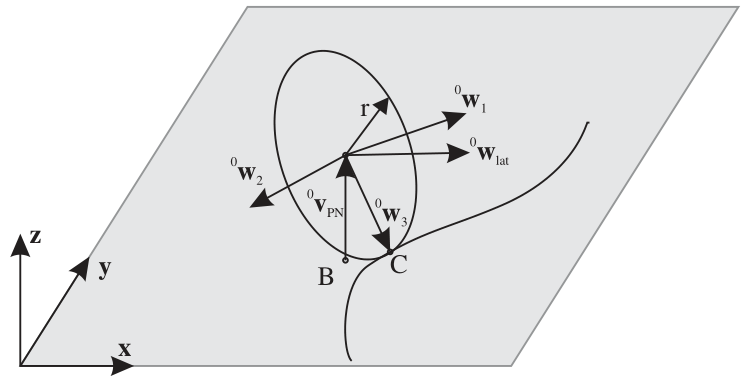
\includegraphics[height=4cm]{figures/ObjectJointRollingDiscSketch.pdf}
    \end{center}
    }
    First, the contact point $\LU{0}{\pv}_{C}$ must be computed.
    With the helper vector,
    \be
      \LU{0}{\xv} = \LU{0}{\wv}_1 \times \LU{0}{\vv_{PN}}
    \ee
    we obtain a disc coordinate system, representing the longitudinal direction,
    \be
      \LU{0}{\wv}_2 = \frac{1}{|\LU{0}{\xv}|} \LU{0}{\xv} 
    \ee
    and the vector to the contact point,
    \be
      \LU{0}{\wv}_3 = \LU{0}{\wv}_1 \times \LU{0}{\wv}_2
    \ee
    The contact point $C$ can be computed from
    \be
      \LU{0}{\pv}_{C} = \LU{0}{\pv}_{m1} + r \cdot \LU{0}{\wv}_3
    \ee
    The velocity of the contact point at the disc is computed from,
    \be
      \LU{0}{\vv}_{Cm1} = \LU{0}{\vv}_{m1} + \LU{0}{\tomega}_{m1} \times (r\cdot \LU{0}{\wv}_3)
    \ee
    If marker 0 body is (moving) rigid body instead of a ground body, the contact point $C$ is reconstructed in 
    body of marker 0,
    \be
      \LU{m0}{\pv}_{C} = \LU{m0,0}{\Rot} (\LU{0}{\pv}_{C} - \LU{0}{\pv}_{m0})
    \ee
    The velocity of the contact point at the marker 0 body reads
    \be
      \LU{0}{\vv}_{Cm0} = \LU{0}{\vv}_{m0} + \LU{0}{\tomega}_{m0} \times \left( \LU{0,m0}{\Rot} \LU{m0}{\pv}_{C} \right)
    \ee
    %
    \mysubsubsubsection{Connector constraint equations}
    \noindent Constraints for \texttt{activeConnector = True}:\\
    %
    The non-holonomic, index 2 constraints for the tangential and normal contact follow from (an index 3 formulation would be possible, but is not implemented yet because of mixing different jacobians)
    \be
      \LU{J1,0}{\Am} \left(\vr{\LU{0}{\vv}_{Cm1,x}}{\LU{0}{\vv}_{Cm1,y}}{\LU{0}{\vv}_{Cm1,z}} - \vr{\LU{0}{\vv}_{Cm0,x}}{\LU{0}{\vv}_{Cm0,y}}{\LU{0}{\vv}_{Cm0,z}} \right) = \Null
    \ee
    \noindent In case that \texttt{activeConnector = False}, the Lagrange multipliers are set to zero:
    \be
      \zv = \Null
    \ee
    Note that since version 1.8.27 the constraints can be turned on/off separately with \texttt{constrainedAxes=[b0,b1,b2]}, in which
    \texttt{b0} represents the flag for lateral motion, \texttt{b1} switches the constraint for forward motion and \texttt{b2} for motion in plane normal direction.
    %%RSTCOMPATIBLE
\vspace{6pt}\par\noindent\rule{\textwidth}{0.4pt}
%
\noindent For examples on ObjectJointRollingDisc see Relevant Examples and TestModels with weblink:
\bi
\item \exuUrl{https://github.com/jgerstmayr/EXUDYN/blob/master/main/pythonDev/Examples/bicycleIftommBenchmark.py}{\texttt{bicycleIftommBenchmark.py}} (Examples/)
\item \exuUrl{https://github.com/jgerstmayr/EXUDYN/blob/master/main/pythonDev/Examples/reinforcementLearningRobot.py}{\texttt{reinforcementLearningRobot.py}} (Examples/)
\item \exuUrl{https://github.com/jgerstmayr/EXUDYN/blob/master/main/pythonDev/TestModels/rollingCoinTest.py}{\texttt{rollingCoinTest.py}} (TestModels/)
\item \exuUrl{https://github.com/jgerstmayr/EXUDYN/blob/master/main/pythonDev/TestModels/rollingDiscTangentialForces.py}{\texttt{rollingDiscTangentialForces.py}} (TestModels/)
\item \exuUrl{https://github.com/jgerstmayr/EXUDYN/blob/master/main/pythonDev/TestModels/rotatingTableTest.py}{\texttt{rotatingTableTest.py}} (TestModels/)

\ei

%
\newpage

%+++++++++++++++++++++++++++++++++++

\mysubsubsection{ObjectJointRevolute2D}
\label{sec:item:ObjectJointRevolute2D}
A revolute joint in 2D; constrains the absolute 2D position of two points given by PointMarkers or RigidMarkers
\vspace{12pt}\\

\noindent \mybold{Additional information for ObjectJointRevolute2D}:
\bi
  \item This \texttt{Object} has/provides the following types = \texttt{Connector}, \texttt{Constraint}
  \item Requested \texttt{Marker} type = \texttt{Position}
  \item {\bf Short name} for Python = \texttt{RevoluteJoint2D}
  \item {\bf Short name} for Python visualization object = \texttt{VRevoluteJoint2D}
\ei\vspace{12pt} \noindent 
The item \mybold{ObjectJointRevolute2D} with type = 'JointRevolute2D' has the following parameters:
\vspace{-0.5cm}\\
\vspace{-0.5cm}\\
%reference manual TABLE
\begin{center}
  \footnotesize
  \begin{longtable}{| p{4.5cm} | p{2.5cm} | p{0.5cm} | p{2.5cm} | p{6cm} |}
    \hline
    \bf Name & \bf type & \bf size & \bf default value & \bf description \\ \hline
    name &     String &      &     '' &     constraints's unique name\\ \hline
    markerNumbers &     ArrayMarkerIndex &     \tabnewline  &     [ invalid [-1], invalid [-1] ] &     \tabnewline list of markers used in connector\\ \hline
    activeConnector &     Bool &      &     True &     flag, which determines, if the connector is active; used to deactivate (temporarily) a connector or constraint\\ \hline
    visualization &     VObjectJointRevolute2D &      &      &     parameters for visualization of item\\ \hline
\end{longtable}
\end{center}

\noindent The item VObjectJointRevolute2D has the following parameters:
%reference manual TABLE
\begin{center}
  \footnotesize
  \begin{longtable}{| p{4.5cm} | p{2.5cm} | p{0.5cm} | p{2.5cm} | p{6cm} |}
    \hline
    \bf Name & \bf type & \bf size & \bf default value & \bf description \\ \hline
    show &     Bool &      &     True &     set true, if item is shown in visualization and false if it is not shown\\ \hline
    drawSize &     float &      &     -1. &     drawing size = radius of revolute joint; size == -1.f means that default connector size is used\\ \hline
    color &     Float4 &      &     [-1.,-1.,-1.,-1.] &     \tabnewline RGBA connector color; if R==-1, use default color\\ \hline
\end{longtable}
\end{center}
\par\noindent\rule{\textwidth}{0.4pt}
\mysubsubsubsection{DESCRIPTION of ObjectJointRevolute2D:}
\label{description_ObjectJointRevolute2D}
\vspace{6pt}\par\noindent\rule{\textwidth}{0.4pt}
%
\noindent For examples on ObjectJointRevolute2D see Relevant Examples and TestModels with weblink:
\bi
\item \exuUrl{https://github.com/jgerstmayr/EXUDYN/blob/master/main/pythonDev/Examples/pendulumGeomExactBeam2D.py}{\texttt{pendulumGeomExactBeam2D.py}} (Examples/)
\item \exuUrl{https://github.com/jgerstmayr/EXUDYN/blob/master/main/pythonDev/Examples/sliderCrank3DwithANCFbeltDrive2.py}{\texttt{sliderCrank3DwithANCFbeltDrive2.py}} (Examples/)
\item \exuUrl{https://github.com/jgerstmayr/EXUDYN/blob/master/main/pythonDev/Examples/ANCFrotatingCable2D.py}{\texttt{ANCFrotatingCable2D.py}} (Examples/)
\item \exuUrl{https://github.com/jgerstmayr/EXUDYN/blob/master/main/pythonDev/Examples/ANCFslidingJoint2D.py}{\texttt{ANCFslidingJoint2D.py}} (Examples/)
\item \exuUrl{https://github.com/jgerstmayr/EXUDYN/blob/master/main/pythonDev/Examples/ANCFslidingJoint2Drigid.py}{\texttt{ANCFslidingJoint2Drigid.py}} (Examples/)
\item \exuUrl{https://github.com/jgerstmayr/EXUDYN/blob/master/main/pythonDev/Examples/beltDriveALE.py}{\texttt{beltDriveALE.py}} (Examples/)
\item \exuUrl{https://github.com/jgerstmayr/EXUDYN/blob/master/main/pythonDev/Examples/beltDriveReevingSystem.py}{\texttt{beltDriveReevingSystem.py}} (Examples/)
\item \exuUrl{https://github.com/jgerstmayr/EXUDYN/blob/master/main/pythonDev/Examples/beltDrivesComparison.py}{\texttt{beltDrivesComparison.py}} (Examples/)
\item \exuUrl{https://github.com/jgerstmayr/EXUDYN/blob/master/main/pythonDev/Examples/chainDriveExample.py}{\texttt{chainDriveExample.py}} (Examples/)
\item \exuUrl{https://github.com/jgerstmayr/EXUDYN/blob/master/main/pythonDev/Examples/doublePendulum2D.py}{\texttt{doublePendulum2D.py}} (Examples/)
\item \exuUrl{https://github.com/jgerstmayr/EXUDYN/blob/master/main/pythonDev/Examples/finiteSegmentMethod.py}{\texttt{finiteSegmentMethod.py}} (Examples/)
\item \exuUrl{https://github.com/jgerstmayr/EXUDYN/blob/master/main/pythonDev/Examples/geneticOptimizationSliderCrank.py}{\texttt{geneticOptimizationSliderCrank.py}} (Examples/)
\item  ...

\item \exuUrl{https://github.com/jgerstmayr/EXUDYN/blob/master/main/pythonDev/TestModels/ANCFbeltDrive.py}{\texttt{ANCFbeltDrive.py}} (TestModels/)
\item \exuUrl{https://github.com/jgerstmayr/EXUDYN/blob/master/main/pythonDev/TestModels/ANCFgeneralContactCircle.py}{\texttt{ANCFgeneralContactCircle.py}} (TestModels/)
\item \exuUrl{https://github.com/jgerstmayr/EXUDYN/blob/master/main/pythonDev/TestModels/ANCFoutputTest.py}{\texttt{ANCFoutputTest.py}} (TestModels/)
\item  ...


\ei

%
\newpage

%+++++++++++++++++++++++++++++++++++

\mysubsubsection{ObjectJointPrismatic2D}
\label{sec:item:ObjectJointPrismatic2D}
A prismatic joint in 2D; allows the relative motion of two bodies, using two RigidMarkers; the vector $\tv_0$ = axisMarker0 is given in local coordinates of the first marker's (body) frame and defines the prismatic axis; the vector $\mathbf{n}_1$ = normalMarker1 is given in the second marker's (body) frame and is the normal vector to the prismatic axis; using the global position vector $\pv_0$ and rotation matrix $\Am_0$ of marker0 and the global position vector $\pv_1$ rotation matrix $\Am_1$ of marker1, the equations for the prismatic joint follow as \be (\pv_1-\pv_0)^T\cdot \Am_1 \cdot \mathbf{n}_1 = 0 \ee  \be (\Am_0 \cdot \tv_0)^T \cdot \Am_1 \cdot \mathbf{n}_1 = 0\ee The lagrange multipliers follow for these two equations $[\lambda_0,\lambda_1]$, in which $\lambda_0$ is the transverse force and $\lambda_1$ is the torque in the joint.
\vspace{12pt}\\

\noindent \mybold{Additional information for ObjectJointPrismatic2D}:
\bi
  \item This \texttt{Object} has/provides the following types = \texttt{Connector}, \texttt{Constraint}
  \item Requested \texttt{Marker} type = \texttt{Position} + \texttt{Orientation}
  \item {\bf Short name} for Python = \texttt{PrismaticJoint2D}
  \item {\bf Short name} for Python visualization object = \texttt{VPrismaticJoint2D}
\ei\vspace{12pt} \noindent 
The item \mybold{ObjectJointPrismatic2D} with type = 'JointPrismatic2D' has the following parameters:
\vspace{-0.5cm}\\
\vspace{-0.5cm}\\
%reference manual TABLE
\begin{center}
  \footnotesize
  \begin{longtable}{| p{4.5cm} | p{2.5cm} | p{0.5cm} | p{2.5cm} | p{6cm} |}
    \hline
    \bf Name & \bf type & \bf size & \bf default value & \bf description \\ \hline
    name &     String &      &     '' &     constraints's unique name\\ \hline
    markerNumbers &     ArrayMarkerIndex &     \tabnewline  &     [ invalid [-1], invalid [-1] ] &     \tabnewline list of markers used in connector\\ \hline
    axisMarker0 &     Vector3D &      &     [1.,0.,0.] &     \tabnewline direction of prismatic axis, given as a 3D vector in Marker0 frame\\ \hline
    normalMarker1 &     Vector3D &      &     [0.,1.,0.] &     \tabnewline direction of normal to prismatic axis, given as a 3D vector in Marker1 frame\\ \hline
    constrainRotation &     Bool &      &     True &     flag, which determines, if the connector also constrains the relative rotation of the two objects; if set to false, the constraint will keep an algebraic equation set equal zero\\ \hline
    activeConnector &     Bool &      &     True &     flag, which determines, if the connector is active; used to deactivate (temporarily) a connector or constraint\\ \hline
    visualization &     VObjectJointPrismatic2D &      &      &     parameters for visualization of item\\ \hline
\end{longtable}
\end{center}

\noindent The item VObjectJointPrismatic2D has the following parameters:
%reference manual TABLE
\begin{center}
  \footnotesize
  \begin{longtable}{| p{4.5cm} | p{2.5cm} | p{0.5cm} | p{2.5cm} | p{6cm} |}
    \hline
    \bf Name & \bf type & \bf size & \bf default value & \bf description \\ \hline
    show &     Bool &      &     True &     set true, if item is shown in visualization and false if it is not shown\\ \hline
    drawSize &     float &      &     -1. &     drawing size = radius of revolute joint; size == -1.f means that default connector size is used\\ \hline
    color &     Float4 &      &     [-1.,-1.,-1.,-1.] &     \tabnewline RGBA connector color; if R==-1, use default color\\ \hline
\end{longtable}
\end{center}
\par\noindent\rule{\textwidth}{0.4pt}
\mysubsubsubsection{DESCRIPTION of ObjectJointPrismatic2D:}
\label{description_ObjectJointPrismatic2D}
\vspace{6pt}\par\noindent\rule{\textwidth}{0.4pt}
%
\noindent For examples on ObjectJointPrismatic2D see Relevant Examples and TestModels with weblink:
\bi
\item \exuUrl{https://github.com/jgerstmayr/EXUDYN/blob/master/main/pythonDev/Examples/sliderCrank3DwithANCFbeltDrive2.py}{\texttt{sliderCrank3DwithANCFbeltDrive2.py}} (Examples/)
\item \exuUrl{https://github.com/jgerstmayr/EXUDYN/blob/master/main/pythonDev/Examples/geneticOptimizationSliderCrank.py}{\texttt{geneticOptimizationSliderCrank.py}} (Examples/)
\item \exuUrl{https://github.com/jgerstmayr/EXUDYN/blob/master/main/pythonDev/TestModels/PARTS_ATEs_moving.py}{\texttt{PARTS\_ATEs\_moving.py}} (TestModels/)
\item \exuUrl{https://github.com/jgerstmayr/EXUDYN/blob/master/main/pythonDev/TestModels/scissorPrismaticRevolute2D.py}{\texttt{scissorPrismaticRevolute2D.py}} (TestModels/)
\item \exuUrl{https://github.com/jgerstmayr/EXUDYN/blob/master/main/pythonDev/TestModels/sliderCrankFloatingTest.py}{\texttt{sliderCrankFloatingTest.py}} (TestModels/)

\ei

%
\newpage

%+++++++++++++++++++++++++++++++++++

\mysubsubsection{ObjectJointSliding2D}
\label{sec:item:ObjectJointSliding2D}
A specialized sliding joint (without rotation) in 2D between a Cable2D (marker1) and a position-based marker (marker0); the data coordinate x[0] provides the current index in slidingMarkerNumbers, and x[1] the local position in the cable element at the beginning of the timestep.
\vspace{12pt}\\

\noindent \mybold{Additional information for ObjectJointSliding2D}:
\bi
  \item This \texttt{Object} has/provides the following types = \texttt{Connector}, \texttt{Constraint}
  \item Requested \texttt{Marker} type = \texttt{\_None}
  \item Requested \texttt{Node} type = \texttt{GenericData}
  \item {\bf Short name} for Python = \texttt{SlidingJoint2D}
  \item {\bf Short name} for Python visualization object = \texttt{VSlidingJoint2D}
\ei\vspace{12pt} \noindent 
The item \mybold{ObjectJointSliding2D} with type = 'JointSliding2D' has the following parameters:
\vspace{-0.5cm}\\
\vspace{-0.5cm}\\
%reference manual TABLE
\begin{center}
  \footnotesize
  \begin{longtable}{| p{4.5cm} | p{2.5cm} | p{0.5cm} | p{2.5cm} | p{6cm} |}
    \hline
    \bf Name & \bf type & \bf size & \bf default value & \bf description \\ \hline
    name &     String &      &     '' &     constraints's unique name\\ \hline
    markerNumbers &     ArrayMarkerIndex &     \tabnewline  &     [ invalid [-1], invalid [-1] ] &     \tabnewline marker m0: position or rigid body marker of mass point or rigid body; marker m1: updated marker to Cable2D element, where the sliding joint currently is attached to; must be initialized with an appropriate (global) marker number according to the starting position of the sliding object; this marker changes with time (PostNewtonStep)\\ \hline
    slidingMarkerNumbers &     ArrayMarkerIndex &     \tabnewline  &     [] &     these markers are used to update marker m1, if the sliding position exceeds the current cable's range; the markers must be sorted such that marker $m_{si}$ at x=cable(i).length is equal to marker(i+1) at x=0 of cable(i+1)\\ \hline
    slidingMarkerOffsets &     Vector &      &     [] &     this list contains the offsets of every sliding object (given by slidingMarkerNumbers) w.r.t. to the initial position (0): marker m0: offset=0, marker m1: offset=Length(cable0), marker m2: offset=Length(cable0)+Length(cable1), ...\\ \hline
    nodeNumber &     NodeIndex &      &     invalid (-1) &     \tabnewline node number of a NodeGenericData for 1 dataCoordinate showing the according marker number which is currently active and the start-of-step (global) sliding position\\ \hline
    classicalFormulation &     Bool &      &     True &     True: uses a formulation with 3 (+1) equations, including the force in sliding direction to be zero; forces in global coordinates, only index 3; False: use local formulation, which only needs 2 (+1) equations and can be used with index 2 formulation\\ \hline
    constrainRotation &     Bool &      &     False &     True: add constraint on rotation of marker m0 relative to slope (if True, marker m0 must be a rigid body marker); False: marker m0 body can rotate freely\\ \hline
    axialForce &     Real &      &     0 &     ONLY APPLIES if classicalFormulation==True; axialForce represents an additional sliding force acting between beam and marker m0 body in axial (beam) direction; this force can be used to drive a body on a beam, but can only be changed with user functions.\\ \hline
    activeConnector &     Bool &      &     True &     flag, which determines, if the connector is active; used to deactivate (temporarily) a connector or constraint\\ \hline
    visualization &     VObjectJointSliding2D &      &      &     parameters for visualization of item\\ \hline
\end{longtable}
\end{center}

\noindent The item VObjectJointSliding2D has the following parameters:
%reference manual TABLE
\begin{center}
  \footnotesize
  \begin{longtable}{| p{4.5cm} | p{2.5cm} | p{0.5cm} | p{2.5cm} | p{6cm} |}
    \hline
    \bf Name & \bf type & \bf size & \bf default value & \bf description \\ \hline
    show &     Bool &      &     True &     set true, if item is shown in visualization and false if it is not shown\\ \hline
    drawSize &     float &      &     -1. &     drawing size = radius of revolute joint; size == -1.f means that default connector size is used\\ \hline
    color &     Float4 &      &     [-1.,-1.,-1.,-1.] &     \tabnewline RGBA connector color; if R==-1, use default color\\ \hline
\end{longtable}
\end{center}
\par\noindent\rule{\textwidth}{0.4pt}
\mysubsubsubsection{DESCRIPTION of ObjectJointSliding2D:}
\label{description_ObjectJointSliding2D}
\paragraph{Information on input parameters:} 
\startTable{input parameter}{symbol}{description see tables above}
\rowTable{markerNumbers}{$[m0,m1]\tp$}{}
\rowTable{slidingMarkerNumbers}{$[m_{s0}, \ldots, m_{sn}]\tp$}{}
\rowTable{slidingMarkerOffsets}{$[d_{s0}, \ldots, d_{sn}]$}{}
\rowTable{nodeNumber}{$n_{GD}$}{}
\rowTable{axialForce}{$f_\mathrm{ax}$}{}
\finishTable

\mybold{The following output variables are available as OutputVariableType in sensors, Get...Output() and other functions}:
\begin{center}
\footnotesize
\begin{longtable}{| p{5cm} | p{5cm} | p{6cm} |} 
\hline
\bf output variable & \bf symbol & \bf description \\ \hline
Position &  & position vector of joint given by marker0\\ \hline
Velocity &  & velocity vector of joint given by marker0\\ \hline
SlidingCoordinate &  & global sliding coordinate along all elements; the maximum sliding coordinate is equivalent to the reference lengths of all sliding elements\\ \hline
Force &  & joint force vector (3D)\\ \hline
\end{longtable}
\end{center}
 \noindent
    \mysubsubsubsection{Definition of quantities}
    %\startTable{input parameter}{symbol}{description}
    %\rowTable{nodeNumber}{$n_{GD}$}{node number of generic data node}
    %\rowTable{markerNumbers[0]}{$m0$}{position-marker of mass point or rigid body (needs to be rigid body marker if constrainRotation==True)}
    %\rowTable{markerNumbers[1]}{$m1$}{marker to a Cable2D element, which is {\bf updated} in every PostNewtonStep; if the sliding body ($m0$) is in the range of all sliding cable elements, $m1$ contains the current marker number, which is active for the sliding joint}
    %\rowTable{slidingMarkerNumbers}{$[m_{s0}, \ldots, m_{sn}]\tp$}{a list of $sn$ (global) marker numbers which are are used to update marker1}
    %\rowTable{slidingMarkerOffsets}{$[d_{s0}, \ldots, d_{sn}]$}{a list of $sn$ scalar offsets, which represent the (reference arc) length of all previous sliding cable elements}
    %\finishTable
    %
    \startTable{intermediate variables}{symbol}{description}
    \rowTable{data node}{$\xv=[x_{data0},\,x_{data1}]\tp$}{coordinates of node with node number $n_{GD}$}
    \rowTable{data coordinate 0}{$x_{data0}$}{the current index in slidingMarkerNumbers}
    \rowTable{data coordinate 1}{$x_{data1}$}{the global sliding coordinate (ranging from 0 to the total length of all sliding elements) at {\bf start-of-step} - beginning of the timestep}
    \rowTable{marker m0 position}{$\LU{0}{\pv}_{m0}$}{current global position which is provided by marker m0}
    \rowTable{marker m0 velocity}{$\LU{0}{\vv}_{m0}$}{current global velocity which is provided by marker m0}
    %
    \rowTable{marker m0 orientation}{$\LU{0,m0}{\Rot}$}{current rotation matrix provided by marker m0 (assumed to be rigid body)}
    \rowTable{marker m0 angular velocity}{$\LU{0}{\tomega}_{m0}$}{current angular velocity vector provided by marker m0 (assumed to be rigid body)}
    %
    \rowTable{cable coordinates}{$\qv_{ANCF,m1}$}{current coordiantes of the ANCF cable element with the current marker $m1$ is referring to}
    \rowTable{sliding position}{$\LUR{0}{\rv}{ANCF} = \Sm(s_{el})\qv_{ANCF,m1}$}{current global position at the ANCF cable element, evaluated at local sliding position $s_{el}$}
    \rowTable{sliding position slope}{$\LURU{0}{\rv}{ANCF}{\prime} = \Sm^\prime(s_{el})\qv_{ANCF,m1} = [r^\prime_0,\,r^\prime_1]\tp$}{current global slope vector of the ANCF cable element, evaluated at local sliding position $s_{el}$}
    \rowTable{sliding velocity}{$\LUR{0}{\vv}{ANCF} = \Sm(s_{el})\dot\qv_{ANCF,m1}$}{current global velocity at the ANCF cable element, evaluated at local sliding position $s_{el}$ ($s_{el}$ not differentiated!!!)}
    \rowTable{sliding velocity slope}{$\LURU{0}{\vv}{ANCF}{\prime} = \Sm^\prime(s_{el})\dot\qv_{ANCF,m1}$}{current global slope velocity vector of the ANCF cable element, evaluated at local sliding position $s_{el}$}
    %
    \rowTable{sliding normal vector}{$\LU{0}{\nv} = [-r^\prime_1,\,r^\prime_0]$}{2D normal vector computed from slope $\rv^\prime=\LURU{0}{\rv}{ANCF}{\prime}$}
    \rowTable{sliding normal velocity vector}{$\LU{0}{\dot\nv} = [-\dot r^\prime_1,\,\dot r^\prime_0]$}{time derivative of 2D normal vector computed from slope velocity $\dot \rv^\prime=\LURU{0}{\dot \rv}{ANCF}{\prime}$}
    %
    \rowTable{algebraic coordinates}{$\zv=[\lambda_0,\,\lambda_1,\, s]\tp$}{algebraic coordinates composed of Lagrange multipliers $\lambda_0$ and $\lambda_1$ (in local cable coordinates: $\lambda_0$ is in axis direction) and the current sliding coordinate $s$, which is local in the current cable element. }
    \rowTable{local sliding coordinate}{$s$}{local incremental sliding coordinate $s$: the (algebraic) sliding coordinate {\bf relative to the start-of-step value}. Thus, $s$ only contains small local increments.}
    \finishTable
    \startTable{output variables}{symbol}{formula}
    \rowTable{Position}{$\LU{0}{\pv}_{m0}$}{current global position of position marker $m0$}
    \rowTable{Velocity}{$\LU{0}{\vv}_{m0}$}{current global velocity of position marker $m0$}
    \rowTable{SlidingCoordinate}{$s_g = s + x_{data1}$}{current value of the global sliding coordinate}
    \rowTable{Force}{$\fv$}{see below}
    \finishTable

    \mysubsubsubsection{Geometric relations}
    %cable
    Assume we have given the sliding coordinate $s$ (e.g., as a guess of the Newton method or beginning of the time step). 
    The element sliding coordinate (in the local coordinates of the current sliding element) is computed as
    \be
      s_{el} = s + x_{data1} - d_{m1} = s_g - d_{m1}.
    \ee
    The vector (=difference; error) between the marker $m0$ and the marker $m1$ (=$\rv_{ANCF}$) positions reads
    \be
      \LU{0}{\Delta\pv} = \LUR{0}{\rv}{ANCF} - \LU{0}{\pv}_{m0}
    \ee
    The vector (=difference; error) between the marker $m0$ and the marker $m1$ velocities reads
    \be
      \LU{0}{\Delta\vv} = \LUR{0}{\dot\rv}{ANCF} - \LU{0}{\vv}_{m0}
    \ee
    %
    %+++++++++++++++++++++++++++++++++++++++++++++
    \mysubsubsubsection{Connector constraint equations (classicalFormulation=True)}
    The 2D sliding joint is implemented having 3 equations (4 if constrainRotation==True, see below), using the special algebraic coordinates $\zv$.
    The algebraic equations read
    \bea
      \LU{0}{\Delta\pv} &=& \Null, \quad \mbox{... two index 3 eqs, ensure sliding body stays at cable}\\
      \left[\lambda_0,\lambda_1\right] \cdot  \LURU{0}{\rv}{ANCF}{\prime} - |\LURU{0}{\rv}{ANCF}{\prime}| \cdot f_\mathrm{ax} &=& 0, \quad \mbox{... one index 1 equ., 
                                               ensure force in sliding dir.~= 0}  \\
    \eea
    No index 2 case exists, because no time derivative exists for $s_{el}$. The jacobian matrices for algebraic and \hac{ODE2} coordinates read
    \be
      \Jm_{AE} = \mr{0}{0}{r^\prime_0} {0}{0}{r^\prime_1} {r^\prime_0}{r^\prime_1}{r^{\prime\prime}_0\lambda_0 + r^{\prime\prime}_1\lambda_1}    %\LURU{0}{\rv}{ANCF}{\prime\prime \mathrm{T}} \vp{\lambda_0}{\lambda_1}}
    \ee
    \be
      \Jm_{ODE2} = \mp{-J_{pos,m0}}{\Sm(s_{el})} {\Null\tp}{\left[\lambda_0,\,\lambda_1\right]\cdot\Sm^\prime(s_{el}) }
    \ee
    if \texttt{activeConnector = False}, the algebraic equations are changed to:
    \bea
      \lambda_0 &=& 0,   \\
      \lambda_1 &=& 0,   \\
      s &=& 0
    \eea
    %the algebraic variables are \be \qv_{AE}=[\lambda_x\;\; \lambda_y \;\; s]^T \ee in which $\lambda_x$ and $\lambda_y$ are the Lagrange multipliers for the position of the sliding joint; 
    %+++++++++++++++++++++++++++++++++++++++++++++
    \mysubsubsubsection{Connector constraint equations (classicalFormulation=False)}
    The 2D sliding joint is implemented having 3 equations (first equation is dummy and could be eliminated; 4 equations if constrainRotation==True, see below), using the special algebraic coordinates $\zv$. 
    The algebraic equations read
    \bea
      \lambda_0 &=& 0, \quad \mbox{... equation not necessary, but can be used for switching to other modes}  \\
      \LU{0}{\Delta\pv\tp} \LU{0}{\nv} &=& 0, \quad \mbox{... equation ensures that sliding body stays at cable centerline; index3}\\
      \LU{0}{\Delta\pv\tp} \LURU{0}{\rv}{ANCF}{\prime} &=& 0. \quad \mbox{... resolves the sliding coordinate $s$; index1 equation!}
    \eea
    In the index 2 case, the second equation reads
    \be
      \LU{0}{\Delta\vv\tp} \LU{0}{\nv}  + \LU{0}{\Delta\pv\tp} \LU{0}{\dot\nv}  = 0
    \ee
    if \texttt{activeConnector = False}, the algebraic equations are changed to:
    \bea
      \lambda_0 &=& 0,   \\
      \lambda_1 &=& 0,   \\
      s &=& 0
    \eea   
    %the algebraic variables are \be \qv_{AE}=[\lambda_x\;\; \lambda_y \;\; s]^T \ee in which $\lambda_x$ and $\lambda_y$ are the Lagrange multipliers for the position of the sliding joint; 
    %
    %+++++++++++++++++++++++++++++++++++++++++++++
    In case that \texttt{constrainRotation = True}, an additional constraint is added for the relative rotation
    between the slope of the cable and the orientation of marker m0 body.
    Assuming that the orientation of marker m0 is a 2D matrix (taking only $x$ and $y$ coordinates), the constraint reads
    \be
      \LURU{0}{\rv}{ANCF}{\prime\mathrm{T}} \LU{0,m0}{\Rot} \vp{0}{1} = 0
    \ee
    The index 2 case follows straightforward to 
    \be
      \LURU{0}{\dot \rv}{ANCF}{\prime\mathrm{T}} \LU{0,m0}{\Rot} \vp{0}{1}  + 
      \LURU{0}{\rv}{ANCF}{\prime\mathrm{T}} \LU{0,m0}{\Rot} \LU{0}{\tilde \tomega}_{m0} \vp{0}{1} = 0
    \ee
    again assuming, that $\LU{0}{\tilde \tomega}_{m0}$ is only a $2 \times 2$ matrix.
    %+++++++++++++++++++++++++++++++++++++++++++++
    \mysubsubsubsection{Post Newton Step}
    After the Newton solver has converged, a PostNewtonStep is performed for the element, which
    updates the marker $m1$ index if necessary.
    \bea
      s_{el} < 0 \quad \ra \quad x_{data0}\;-\!\!=1 \nonumber\\
      s_{el} > L \quad \ra \quad x_{data0}\;+\!\!=1
    \eea
    Furthermore, it is checked, if $x_{data0}$ becomes smaller than zero, which raises a warning and keeps $x_{data0}=0$.
    The same results if $x_{data0}\ge sn$, then $x_{data0} = sn$.
    Finally, the data coordinate is updated in order to provide the starting value for the next step,
    \be
      x_{data1} \;+\!\!= s.
    \ee
    %the data coordinates are \be \qv_{Data} = [i_{marker} \;\; s_{0}]^T \ee in which $i_{marker}$ is the current local index to the slidingMarkerNumber list and  $s_{0}$ is the sliding coordinate (which is the total sliding length along all cable elements in the cableMarkerNumber list) at the beginning of the solution step.
    %%RSTCOMPATIBLE
\vspace{6pt}\par\noindent\rule{\textwidth}{0.4pt}
%
\noindent For examples on ObjectJointSliding2D see Relevant Examples and TestModels with weblink:
\bi
\item \exuUrl{https://github.com/jgerstmayr/EXUDYN/blob/master/main/pythonDev/Examples/ANCFmovingRigidbody.py}{\texttt{ANCFmovingRigidbody.py}} (Examples/)
\item \exuUrl{https://github.com/jgerstmayr/EXUDYN/blob/master/main/pythonDev/Examples/ANCFslidingJoint2D.py}{\texttt{ANCFslidingJoint2D.py}} (Examples/)
\item \exuUrl{https://github.com/jgerstmayr/EXUDYN/blob/master/main/pythonDev/Examples/ANCFslidingJoint2Drigid.py}{\texttt{ANCFslidingJoint2Drigid.py}} (Examples/)
\item \exuUrl{https://github.com/jgerstmayr/EXUDYN/blob/master/main/pythonDev/Examples/ANCFswitchingSlidingJoint2D.py}{\texttt{ANCFswitchingSlidingJoint2D.py}} (Examples/)
\item \exuUrl{https://github.com/jgerstmayr/EXUDYN/blob/master/main/pythonDev/TestModels/modelUnitTests.py}{\texttt{modelUnitTests.py}} (TestModels/)

\ei

%
\newpage

%+++++++++++++++++++++++++++++++++++

\mysubsubsection{ObjectJointALEMoving2D}
\label{sec:item:ObjectJointALEMoving2D}
A specialized axially moving joint (without rotation) in 2D between a ALE Cable2D (marker1) and a position-based marker (marker0); ALE=Arbitrary Lagrangian Eulerian; the data coordinate x[0] provides the current index in slidingMarkerNumbers, and the \hac{ODE2} coordinate q[0] provides the (given) moving coordinate in the cable element.
\vspace{12pt}\\

\noindent \mybold{Additional information for ObjectJointALEMoving2D}:
\bi
  \item This \texttt{Object} has/provides the following types = \texttt{Connector}, \texttt{Constraint}
  \item Requested \texttt{Marker} type = \texttt{\_None}
  \item Requested \texttt{Node} type: read detailed information of item
  \item {\bf Short name} for Python = \texttt{ALEMovingJoint2D}
  \item {\bf Short name} for Python visualization object = \texttt{VALEMovingJoint2D}
\ei\vspace{12pt} \noindent 
The item \mybold{ObjectJointALEMoving2D} with type = 'JointALEMoving2D' has the following parameters:
\vspace{-0.5cm}\\
\vspace{-0.5cm}\\
%reference manual TABLE
\begin{center}
  \footnotesize
  \begin{longtable}{| p{4.5cm} | p{2.5cm} | p{0.5cm} | p{2.5cm} | p{6cm} |}
    \hline
    \bf Name & \bf type & \bf size & \bf default value & \bf description \\ \hline
    name &     String &      &     '' &     constraints's unique name\\ \hline
    markerNumbers &     ArrayMarkerIndex &     \tabnewline  &     [ invalid [-1], invalid [-1] ] &     \tabnewline marker m0: position-marker of mass point or rigid body; marker m1: updated marker to ANCF Cable2D element, where the sliding joint currently is attached to; must be initialized with an appropriate (global) marker number according to the starting position of the sliding object; this marker changes with time (PostNewtonStep)\\ \hline
    slidingMarkerNumbers &     ArrayMarkerIndex &     \tabnewline  &     [] &     a list of sn (global) marker numbers which are are used to update marker1\\ \hline
    slidingMarkerOffsets &     Vector &      &     [] &     this list contains the offsets of every sliding object (given by slidingMarkerNumbers) w.r.t. to the initial position (0): marker0: offset=0, marker1: offset=Length(cable0), marker2: offset=Length(cable0)+Length(cable1), ...\\ \hline
    slidingOffset &     Real &      &     0. &     sliding offset list [SI:m]: a list of sn scalar offsets, which represent the (reference arc) length of all previous sliding cable elements\\ \hline
    nodeNumbers &     ArrayNodeIndex &      &     [ invalid [-1], invalid [-1] ] &     \tabnewline node number of NodeGenericData (GD) with one data coordinate and of NodeGenericODE2 (ALE) with one \hac{ODE2} coordinate\\ \hline
    usePenaltyFormulation &     Bool &      &     False &     flag, which determines, if the connector is formulated with penalty, but still using algebraic equations (IsPenaltyConnector() still false)\\ \hline
    penaltyStiffness &     Real &      &     0. &     penalty stiffness [SI:N/m] used if usePenaltyFormulation=True\\ \hline
    activeConnector &     Bool &      &     True &     flag, which determines, if the connector is active; used to deactivate (temporarily) a connector or constraint\\ \hline
    visualization &     VObjectJointALEMoving2D &      &      &     parameters for visualization of item\\ \hline
\end{longtable}
\end{center}

\noindent The item VObjectJointALEMoving2D has the following parameters:
%reference manual TABLE
\begin{center}
  \footnotesize
  \begin{longtable}{| p{4.5cm} | p{2.5cm} | p{0.5cm} | p{2.5cm} | p{6cm} |}
    \hline
    \bf Name & \bf type & \bf size & \bf default value & \bf description \\ \hline
    show &     Bool &      &     True &     set true, if item is shown in visualization and false if it is not shown\\ \hline
    drawSize &     float &      &     -1. &     drawing size = radius of revolute joint; size == -1.f means that default connector size is used\\ \hline
    color &     Float4 &      &     [-1.,-1.,-1.,-1.] &     \tabnewline RGBA connector color; if R==-1, use default color\\ \hline
\end{longtable}
\end{center}
\par\noindent\rule{\textwidth}{0.4pt}
\mysubsubsubsection{DESCRIPTION of ObjectJointALEMoving2D:}
\label{description_ObjectJointALEMoving2D}
\paragraph{Information on input parameters:} 
\startTable{input parameter}{symbol}{description see tables above}
\rowTable{markerNumbers}{$[m0,\,m1]\tp$}{}
\rowTable{slidingMarkerNumbers}{$[m_{s0}, \ldots, m_{sn}]\tp$}{}
\rowTable{slidingMarkerOffsets}{$[d_{s0}, \ldots, d_{sn}]$}{}
\rowTable{slidingOffset}{$s_{off}$}{}
\rowTable{nodeNumbers}{$[n_{GD}, n_{ALE}]$}{}
\rowTable{penaltyStiffness}{$k$}{}
\finishTable

\mybold{The following output variables are available as OutputVariableType in sensors, Get...Output() and other functions}:
\begin{center}
\footnotesize
\begin{longtable}{| p{5cm} | p{5cm} | p{6cm} |} 
\hline
\bf output variable & \bf symbol & \bf description \\ \hline
Position & $\LU{0}{\pv}_{m0}$ & current global position of position marker $m0$\\ \hline
Velocity & $\LU{0}{\vv}_{m0}$ & current global velocity of position marker $m0$\\ \hline
SlidingCoordinate & $s_g = q_{ALE} + s_{off}$ & current value of the global sliding ALE coordinate, including offset; note that reference coordinate of $q_{ALE}$ is ignored!\\ \hline
Coordinates & $[x_{data0},\,q_{ALE}]\tp$ & provides two values: [0] = current sliding marker index, [1] = ALE sliding coordinate\\ \hline
Coordinates\_t & $[\dot q_{ALE}]\tp$ & provides ALE sliding velocity\\ \hline
Force & $\fv$ & joint force vector (3D)\\ \hline
\end{longtable}
\end{center}
 \noindent
    \mysubsubsubsection{Definition of quantities}
    %
    \startTable{intermediate variables}{symbol}{description}
    \rowTable{generic data node}{$\xv=[x_{data0}]\tp$}{coordinates of node with node number $n_{GD}$}
    \rowTable{generic \hac{ODE2} node}{$\qv=[q_{0}]\tp$}{coordinates of node with node number $n_{ALE}$, which is shared with all ALE-ANCF and ALE sliding joint objects}
    \rowTable{data coordinate}{$x_{data0}$}{the current index in slidingMarkerNumbers}
    \rowTable{ALE coordinate}{$q_{ALE} = q_{0}$}{current ALE coordinate (in fact this is the Eulerian coordinate in the ALE formulation); note that reference coordinate of $q_{ALE}$ is ignored!}
    \rowTable{marker m0 position}{$\LU{0}{\pv}_{m0}$}{current global position which is provided by marker m0}
    \rowTable{marker m0 velocity}{$\LU{0}{\vv}_{m0}$}{current global velocity which is provided by marker m0}
    %
    \rowTable{cable coordinates}{$\qv_{ANCF,m1}$}{current coordiantes of the ANCF cable element with the current marker $m1$ is referring to}
    \rowTable{sliding position}{$\LUR{0}{\rv}{ANCF} = \Sm(s_{el})\qv_{ANCF,m1}$}{current global position at the ANCF cable element, evaluated at local sliding position $s_{el}$}
    \rowTable{sliding position slope}{$\LURU{0}{\rv}{ANCF}{\prime} = \Sm^\prime(s_{el})\qv_{ANCF,m1}$}{current global slope vector of the ANCF cable element, evaluated at local sliding position $s_{el}$}
    \rowTable{sliding velocity}{$\LUR{0}{\vv}{ANCF} = \Sm(s_{el})\dot\qv_{ANCF,m1} + \dot q_{ALE} \LURU{0}{\rv}{ANCF}{\prime}$}{current global velocity at the ANCF cable element, evaluated at local sliding position $s_{el}$, including convective term}
    %
    \rowTable{sliding normal vector}{$\LU{0}{\nv} = [-r^\prime_1,\,r^\prime_0]$}{2D normal vector computed from slope $\rv^\prime=\LURU{0}{\rv}{ANCF}{\prime}$}
    %\rowTable{sliding normal vector}{$\LU{0}{\dot\nv} = [-\dot r^\prime_1,\,\dot r^\prime_0]$}{time derivative of 2D normal vector computed from slope velocity $\dot \rv^\prime=\LURU{0}{\dot \rv}{ANCF}{\prime}$}
    %
    \rowTable{algebraic variables}{$\zv=[\lambda_0,\,\lambda_1]\tp$}{algebraic variables (Lagrange multipliers) according to the algebraic equations }
    \finishTable
    %\startTable{output variables}{symbol}{formula}
    %\rowTable{Position}{$\LU{0}{\pv}_{m0}$}{current global position of position marker $m0$}
    %\rowTable{Velocity}{$\LU{0}{\vv}_{m0}$}{current global velocity of position marker $m0$}
    %\rowTable{SlidingCoordinate}{$s_g = q_{ALE} + s_{off}$}{current value of the global sliding ALE coordinate, including offset; note that reference coordinate of $q_{ALE}$ is ignored!}
    %\rowTable{Coordinates}{$[x_{data0},\,q_{ALE}]\tp$}{}
    %\rowTable{Coordinates\_t}{$[\dot q_{ALE}]\tp$}{}
    %\rowTable{Force}{$\fv$}{see below}
    %\finishTable

    \mysubsubsubsection{Geometric relations}
    The element sliding coordinate (in the local coordinates of the current sliding element) is computed from the ALE coordinate
    \be
      s_{el} = q_{ALE} + s_{off} - d_{m1} = s_g - d_{m1}.
    \ee
    For the description of the according quantities, see the description above. The distance $d_{m1}$ is obtained from the \texttt{slidingMarkerOffsets} list, using the current (local) index $x_{data0}$.
    The vector (=difference; error) between the marker $m0$ and the marker $m1$ (=$\rv_{ANCF}$) positions reads
    \be
      \LU{0}{\Delta\pv} = \LUR{0}{\rv}{ANCF} - \LU{0}{\pv}_{m0}
    \ee
    Note that $\LU{0}{\pv}_{m0}$ represents the current position of the marker $m0$, which could represent the midpoint of a mass sliding along the beam.
    The position $\LUR{0}{\rv}{ANCF}$ is computed from the beam represented by marker $m1$, using the local beam coordinate $x=s_{el}$. 
    The marker and the according beam finite element changes during movement using the list \texttt{slidingMarkerNumbers} and the index is updated in the PostNewtonStep.
    The vector (=difference; error) between the marker $m0$ and the marker $m1$ velocities reads
    \be
      \LU{0}{\Delta\vv} = \LUR{0}{\vv}{ANCF} - \LU{0}{\vv}_{m0}
    \ee
    %
    \ignoreRST{
    \begin{figure}[tbh]
        \label{fig:ObjectJointALEmoving2D}
        \begin{center}
            \includegraphics[height=4cm]{figures/ObjectJointALEmoving2D.pdf}
        \end{center}
        \caption{Geometrical relations for ALE sliding joint.}
    \end{figure}
    }
    %+++++++++++++++++++++++++++++++++++++++++++++
    \mysubsubsubsection{Connector constraint equations}
    The 2D sliding joint is implemented having 2 equations, using the Lagrange multipliers $\zv$. 
    The algebraic (index 3) equations read
    \be
      \LU{0}{\Delta\pv} = 0
    \ee
    Note that the Lagrange multipliers $[\lambda_0,\,\lambda_1]\tp$are the global forces in the joint.
    In the index 2 case the algebraic equations read
    \be
      \LU{0}{\Delta\vv} = 0
    \ee
    If \texttt{usePenalty = True}, the algebraic equations are changed to:
    \be
      \LU{0}{\Delta \pv} - \frac 1 k \zv = 0.
    \ee
    %
    %not realized yet, because \hac{AE} Jacobian becomes involved:
    %If \texttt{usePenaltyFormulation = True}, the algebraic equations are changed to:
    %\bea
    %  k_1 \LURU{0}{\rv}{ANCF}{\prime \mathrm{T}}   \LU{0}{\Delta\pv} - \lambda_0 &=& 0, \nonumber \\
    %  k_2 \LU{0}{\nv\tp}   \LU{0}{\Delta\pv}  - \lambda_1 &=& 0.
    %\eea
    %Note that in this case, the Lagrange multipliers $[\lambda_0,\,\lambda_1]\tp$are the local ($m1$) forces in the joint.

    \noindent If \texttt{activeConnector = False}, the algebraic equations are changed to:
    \bea
      \lambda_0 &=& 0,   \\
      \lambda_1 &=& 0.
    \eea   
    %
    %+++++++++++++++++++++++++++++++++++++++++++++
    \mysubsubsubsection{Post Newton Step}
    After the Newton solver has converged, a PostNewtonStep is performed for the element, which
    updates the marker $m1$ index if necessary.
    \bea
      s_{el} < 0 \quad \ra \quad x_{data0} \;-\!\!=1 \nonumber\\
      s_{el} > L \quad \ra \quad x_{data0} \;+\!\!=1
    \eea
    Furthermore, it is checked, if $x_{data0}$ becomes smaller than zero, which raises a warning and keeps $x_{data0}=0$.
    The same results if $x_{data0}\ge sn$, then $x_{data0} = sn$.
    Finally, the data coordinate is updated in order to provide the starting value for the next step,
    \be
      x_{data1} \;+\!\!= s.
    \ee
    %%RSTCOMPATIBLE
\vspace{6pt}\par\noindent\rule{\textwidth}{0.4pt}
%
\noindent For examples on ObjectJointALEMoving2D see Relevant Examples and TestModels with weblink:
\bi
\item \exuUrl{https://github.com/jgerstmayr/EXUDYN/blob/master/main/pythonDev/Examples/ANCFmovingRigidbody.py}{\texttt{ANCFmovingRigidbody.py}} (Examples/)
\item \exuUrl{https://github.com/jgerstmayr/EXUDYN/blob/master/main/pythonDev/TestModels/ANCFmovingRigidBodyTest.py}{\texttt{ANCFmovingRigidBodyTest.py}} (TestModels/)

\ei

%

\newpage
%+++++++++++++++++++++++++++++++
%+++++++++++++++++++++++++++++++
\mysubsection{Objects (Connector)}
A Connector is a special Object, which links two or more markers. A Connector which is not a Constraint, is a force element (e.g., spring-damper) or a penalty based joint.
%++++++

%+++++++++++++++++++++++++++++++++++

\mysubsubsection{ObjectConnectorSpringDamper}
\label{sec:item:ObjectConnectorSpringDamper}
An simple spring-damper element with additional force; connects to position-based markers.
\vspace{12pt}\\

\noindent \mybold{Additional information for ObjectConnectorSpringDamper}:
\bi
  \item This \texttt{Object} has/provides the following types = \texttt{Connector}
  \item Requested \texttt{Marker} type = \texttt{Position}
  \item {\bf Short name} for Python = \texttt{SpringDamper}
  \item {\bf Short name} for Python visualization object = \texttt{VSpringDamper}
\ei\vspace{12pt} \noindent 
The item \mybold{ObjectConnectorSpringDamper} with type = 'ConnectorSpringDamper' has the following parameters:
\vspace{-0.5cm}\\
\vspace{-0.5cm}\\
%reference manual TABLE
\begin{center}
  \footnotesize
  \begin{longtable}{| p{4.5cm} | p{2.5cm} | p{0.5cm} | p{2.5cm} | p{6cm} |}
    \hline
    \bf Name & \bf type & \bf size & \bf default value & \bf description \\ \hline
    name &     String &      &     '' &     connector's unique name\\ \hline
    markerNumbers &     ArrayMarkerIndex &     \tabnewline  &     [ invalid [-1], invalid [-1] ] &     \tabnewline list of markers used in connector\\ \hline
    referenceLength &     UReal &      &     0. &     reference length [SI:m] of spring\\ \hline
    stiffness &     UReal &      &     0. &     stiffness [SI:N/m] of spring; force acts against (length-initialLength)\\ \hline
    damping &     UReal &      &     0. &     damping [SI:N/(m s)] of damper; force acts against d/dt(length)\\ \hline
    force &     Real &      &     0. &     added constant force [SI:N] of spring; scalar force; f=1 is equivalent to reducing initialLength by 1/stiffness; f > 0: tension; f < 0: compression; can be used to model actuator force\\ \hline
    velocityOffset &     Real &      &     0. &     velocity offset [SI:m/s] of damper, being equivalent to time change of reference length\\ \hline
    activeConnector &     Bool &      &     True &     flag, which determines, if the connector is active; used to deactivate (temporarily) a connector or constraint\\ \hline
    springForceUserFunction &     PyFunctionMbsScalarIndexScalar5 &     \tabnewline  &     \tabnewline 0 &     A Python function which defines the spring force with parameters; the Python function will only be evaluated, if activeConnector is true, otherwise the SpringDamper is inactive; see description below\\ \hline
    visualization &     VObjectConnectorSpringDamper &      &      &     parameters for visualization of item\\ \hline
\end{longtable}
\end{center}

\noindent The item VObjectConnectorSpringDamper has the following parameters:
%reference manual TABLE
\begin{center}
  \footnotesize
  \begin{longtable}{| p{4.5cm} | p{2.5cm} | p{0.5cm} | p{2.5cm} | p{6cm} |}
    \hline
    \bf Name & \bf type & \bf size & \bf default value & \bf description \\ \hline
    show &     Bool &      &     True &     set true, if item is shown in visualization and false if it is not shown\\ \hline
    drawSize &     float &      &     -1. &     drawing size = diameter of spring; size == -1.f means that default connector size is used\\ \hline
    color &     Float4 &      &     [-1.,-1.,-1.,-1.] &     \tabnewline RGBA connector color; if R==-1, use default color\\ \hline
\end{longtable}
\end{center}
\par\noindent\rule{\textwidth}{0.4pt}
\mysubsubsubsection{DESCRIPTION of ObjectConnectorSpringDamper:}
\label{description_ObjectConnectorSpringDamper}
\paragraph{Information on input parameters:} 
\startTable{input parameter}{symbol}{description see tables above}
\rowTable{markerNumbers}{$[m0,m1]\tp$}{}
\rowTable{referenceLength}{$L_0$}{}
\rowTable{stiffness}{$k$}{}
\rowTable{damping}{$d$}{}
\rowTable{force}{$f_{a}$}{}
\rowTable{velocityOffset}{$\dot L_0$}{}
\rowTable{springForceUserFunction}{$\mathrm{UF} \in \Rcal$}{}
\finishTable

\mybold{The following output variables are available as OutputVariableType in sensors, Get...Output() and other functions}:
\begin{center}
\footnotesize
\begin{longtable}{| p{5cm} | p{5cm} | p{6cm} |} 
\hline
\bf output variable & \bf symbol & \bf description \\ \hline
Distance &  & distance between both points\\ \hline
Displacement &  & relative displacement between both points\\ \hline
Velocity &  & relative velocity between both points\\ \hline
Force & $\fv$ & 3D spring-damper force vector\\ \hline
ForceLocal & $f_{SD}$ & scalar spring-damper force\\ \hline
\end{longtable}
\end{center}
 \noindent
    \mysubsubsubsection{Definition of quantities}
    \startTable{intermediate variables}{symbol}{description}
    \rowTable{marker m0 position}{$\LU{0}{\pv}_{m0}$}{current global position which is provided by marker m0}
    \rowTable{marker m1 position}{$\LU{0}{\pv}_{m1}$}{}
    \rowTable{marker m0 velocity}{$\LU{0}{\vv}_{m0}$}{current global velocity which is provided by marker m0}
    \rowTable{marker m1 velocity}{$\LU{0}{\vv}_{m1}$}{}
    \rowTable{time derivative of distance}{$\dot L$}{$\Delta\! \LU{0}{\vv}\tp \vv_{f}$}
    \finishTable
    \startTable{output variables}{symbol}{formula}
    \rowTable{Displacement}{$\Delta\! \LU{0}{\pv}$}{$\LU{0}{\pv}_{m1} - \LU{0}{\pv}_{m0}$}
    \rowTable{Velocity}{$\Delta\! \LU{0}{\vv}$}{$\LU{0}{\vv}_{m1} - \LU{0}{\vv}_{m0}$}
    \rowTable{Distance}{$L$}{$|\Delta\! \LU{0}{\pv}|$}
    \rowTable{Force}{$\fv$}{see below}
    \finishTable
    %
    %++++++++++++++++++++++++++++++++++++++++++++++++++++++++++
    \mysubsubsubsection{Connector forces}
    %
    The unit vector in force direction reads (raises SysError if $L=0$),
    \be
      \vv_{f} = \frac{1}{L} \Delta\! \LU{0}{\pv}
    \ee
    If \texttt{activeConnector = True}, the scalar spring force is computed as
    \be
      f_{SD} = k\cdot(L-L_0) + d \cdot(\dot L -\dot L_0)+ f_{a}
    \ee
    If the springForceUserFunction $\mathrm{UF}$ is defined, $\fv$ instead becomes ($t$ is current time)
    \be
      f_{SD} = \mathrm{UF}(mbs, t, i_N, L-L_0, \dot L - \dot L_0, k, d, f_{a})
    \ee
    and \texttt{iN} represents the itemNumber (=objectNumber). Note that, if \texttt{activeConnector = False}, $f_{SD}$ is set to zero.

    The vector of the spring-damper force applied at both markers finally reads
    \be
      \fv = f_{SD}\vv_{f}
    \ee
    The virtual work of the connector force is computed from the virtual displacement 
    \be
      \delta \Delta\! \LU{0}{\pv} = \delta \LU{0}{\pv}_{m1} - \delta \LU{0}{\pv}_{m0} \eqComma
    \ee
    and the virtual work (note the transposed version here, because the resulting generalized forces shall be a column vector),
    \be
      \delta W_{SD} = \fv \delta \Delta\! \LU{0}{\pv} 
      = \left( k\cdot(L-L_0) + d \cdot (\dot L - \dot L_0) + f_{a} \right) \left(\delta \LU{0}{\pv}_{m1} - \delta \LU{0}{\pv}_{m0} \right)\tp \vv_{f} 
      \eqDot
    \ee
    The generalized (elastic) forces thus result from
    \be
      \Qm_{SD} = \frac{\partial \LU{0}{\pv}}{\partial \qv_{SD}\tp} \fv 
      \eqComma
    \ee
    and read for the markers $m0$ and $m1$,
    \be
      \Qm_{SD, m0} 
      = -\left( k\cdot(L-L_0) + d \cdot (\dot L - \dot L_0) + f_{a} \right) \Jm_{pos,m0}\tp \vv_{f} , \quad
      \Qm_{SD, m1} 
      = \left( k\cdot(L-L_0) + d \cdot (\dot L - \dot L_0)+ f_{a} \right) \Jm_{pos,m1}\tp \vv_{f} 
      \eqComma    
    \ee
    where $\Jm_{pos,m1}$ represents the derivative of marker $m1$ w.r.t.\ its associated coordinates $\qv_{m1}$, analogously $\Jm_{pos,m0}$.
    %
    \mysubsubsubsection{Connector Jacobian}
    The position-level jacobian for the connector, involving all coordinates associated with markers $m0$ and $m1$, follows from 
    \be
      \Jm_{SD} = \mp{\frac{\partial \Qm_{SD, m0}}{\partial \qv_{m0}} }{\frac{\partial \Qm_{SD, m0}}{\partial \qv_{m1}}}
                    {\frac{\partial \Qm_{SD, m0}}{\partial \qv_{m1}} }{\frac{\partial \Qm_{SD, m1}}{\partial \qv_{m1}}}
    \ee
    and the velocity level jacobian reads
    \be
      \Jm_{SD,t} = \mp{\frac{\partial \Qm_{SD, m0}}{\partial \dot \qv_{m0}} }{\frac{\partial \Qm_{SD, m0}}{\partial \dot \qv_{m1}}}
                    {\frac{\partial \Qm_{SD, m0}}{\partial \dot \qv_{m1}} }{\frac{\partial \Qm_{SD, m1}}{\partial \dot \qv_{m1}}}
    \ee
    The sub-Jacobians follow from
    \be
      \frac{\partial \Qm_{SD, m0}}{\partial \qv_{m0}} = 
       -\frac{\partial \Jm_{pos,m0}\tp }{\partial \qv_{m0}} \vv_{f} \left( k\cdot(L-L_0) + d \cdot(\dot L - \dot L_0) + f_{a} \right) 
       -\Jm_{pos,m0}\tp \frac{\partial \vv_{f} \left( k\cdot(L-L_0) + d \cdot(\dot L - \dot L_0) + f_{a} \right)   }{\partial \qv_{m0}} 
    \ee
    in which the term $\frac{\partial \Jm_{pos,m0}\tp }{\partial \qv_{m0}}$ is computed from a special function provided by markers, that
    compute the derivative of the marker jacobian times a constant vector, in this case the spring force $\fv$; this jacobian term is usually less  
    dominant, but is included in the numerical as well as the analytical derivatives, see the general jacobian computation information.
    
    The other term, which is the dominant term, is computed as (dependence of velocity term on position coordinates and $\dot L_0$ term neglected),
    \bea
      \frac{\partial \Qm_{SD, m0}}{\partial \qv_{m0}}
      &=& -\Jm_{pos,m0}\tp \frac{\partial \vv_{f} \left( k\cdot(L-L_0) + d \cdot(\dot L - \dot L_0) + f_{a} \right)   }{\partial \qv_{m0}}
      \nonumber \\
      &=& -\Jm_{pos,m0}\tp \frac{\partial  \left( k\cdot \left( \Delta\! \LU{0}{\pv} - L_0 \vv_{f} \right)+ \vv_{f} \left(d \cdot \vv_{f}\tp \Delta\! \LU{0}{\vv}  + f_{a} \right) \right)   }{\partial \qv_{m0}} 
      \nonumber \\
      &\approx& \Jm_{pos,m0}\tp \left(k\cdot \Im - k  \frac{L_0}{L}\left(\Im - \LU{0}{\vv_{f}} \otimes \LU{0}{\vv_{f}} \right)  +\frac{1}{L}\left(\Im - \LU{0}{\vv_{f}} \otimes \LU{0}{\vv_{f}} \right) \left(d \cdot \vv_{f}\tp \Delta\! \LU{0}{\vv}  + f_{a} \right) \right. \nonumber \\
      &&\left. + d \LU{0}{\vv_{f}} \otimes \left(\frac{1}{L}\left(\Im - \LU{0}{\vv_{f}} \otimes 
      \LU{0}{\vv_{f}} \right) \LU{0}{\vv_{f}} \right) \right)
      \LU{0}{\Jm_{pos,m0}}
    \eea
    %+++++++++++++++++++++++++++++++++++++++++++
    Alternatively (again $\dot L_0$ term neglected):
    \bea
      \frac{\partial \Qm_{SD, m0}}{\partial \qv_{m0}}
      &=& -\Jm_{pos,m0}\tp \frac{\partial \vv_{f} \left( k\cdot(L-L_0) + d \cdot(\dot L - \dot L_0) + f_{a} \right)   }{\partial \qv_{m0}}
      \nonumber \\
      %+++
      &=& \Jm_{pos,m0}\tp \frac{1}{L}\left(\Im - \LU{0}{\vv_{f}} \otimes \LU{0}{\vv_{f}} \right)
          \left( k\cdot(L-L_0) + d \cdot(\dot L - \dot L_0) + f_{a} \right) \Jm_{pos,m0}
      \nonumber \\
      && +\Jm_{pos,m0}\tp \LU{0}{\vv_{f}}
          \otimes \left( k\cdot \LU{0}{\vv_{f}} + d \cdot\Delta\! \LU{0}{\vv} \frac{1}{L}\left(\Im - \LU{0}{\vv_{f}} \otimes \LU{0}{\vv_{f}} \right) 
          \right) \Jm_{pos,m0} - d \Jm_{pos,m0}\tp \LU{0}{\vv_{f}} \otimes \LU{0}{\vv_{f}} \frac{\partial \Delta\! \LU{0}{\vv}}{\partial \qv_{m0}}  \nonumber \\
      %+++
      &=& \Jm_{pos,m0}\tp \left(\frac{f_{SD}}{L}\left(\Im - \LU{0}{\vv_{f}} \otimes \LU{0}{\vv_{f}} \right)
           + k \LU{0}{\vv_{f}} \otimes \LU{0}{\vv_{f}} + 
          \frac{d}{L} \left(\LU{0}{\vv_{f}} \otimes \Delta\! \LU{0}{\vv}\right) 
                 \cdot \left(\Im - \LU{0}{\vv_{f}} \otimes \LU{0}{\vv_{f}} \right) + ...!
          \right) \Jm_{pos,m0} 
    \eea
    %+++++++++++++++++++++++++++++++++++++++++++
    Noting that $\frac{\partial \vv_{f} }{\partial \qv_{m0}} = 
    -\frac{1}{L}\left(\Im - \LU{0}{\vv_{f}} \otimes \LU{0}{\vv_{f}} \right) \LU{0}{\Jm_{pos,m0}}$ and 
    $\frac{\partial \vv_{f} }{\partial \qv_{m1}} = 
    \frac{1}{L}\left(\Im - \LU{0}{\vv_{f}} \otimes \LU{0}{\vv_{f}} \right) \LU{0}{\Jm_{pos,m1}}$.
    %
    The Jacobian w.r.t.\ velocity coordinates follows as
    \bea
      \frac{\partial \Qm_{SD, m0}}{\partial \dot \qv_{m0}}
      &=& -\Jm_{pos,m0}\tp \frac{\partial \vv_{f} \left( k\cdot(L-L_0) + d \cdot(\dot L - \dot L_0) + f_{a} \right)   }{\partial \dot \qv_{m0}}
      \nonumber \\
      &=& \Jm_{pos,m0}\tp \left(d \vv_{f} \otimes \vv_{f} \right) \LU{0}{\Jm_{pos,m0}} 
    \eea
    Note that in case that $L=0$, the term $\frac{1}{L} \left(\Im - \LU{0}{\vv_{f}} \otimes \LU{0}{\vv_{f}} \right)$ is replaced
    by the unit matrix, in order to avoid zero (singular) jacobian; this is a workaround and should only occur in exceptional cases.
    
    The term $\frac{\partial \Delta\! \LU{0}{\vv}}{\partial \qv_{m0}}$, which is important for large damping, yields
    \be
      \frac{\partial \Delta\! \LU{0}{\vv}}{\partial \qv_{m0}} = 
      \frac{\partial \Jm_{pos,m0} \dot \qv_{m0}}{\partial \qv_{m0}}=
      \frac{\partial \Jm_{pos,m0} }{\partial \qv_{m0}} \dot \qv_{m0}
    \ee
    The latter term is currently neglected.
    
    Jacobians for markers $m1$ and mixed $m0$/$m1$ terms follow analogously.
    %++++++++++++++++++++++++++++++++++++++++++++++++++++++++++
    \userFunction{springForceUserFunction(mbs, t, itemNumber, deltaL, deltaL\_t, stiffness, damping, force)}
    A user function, which computes the spring force depending on time, object variables (deltaL, deltaL\_t) and 
    object parameters (stiffness, damping, force).
    The object variables are provided to the function using the current values of the SpringDamper object.
    Note that itemNumber represents the index of the object in mbs, which can be used to retrieve additional data from the object through
    \texttt{mbs.GetObjectParameter(itemNumber, ...)}, see the according description of \texttt{GetObjectParameter}.
    %
    \startTable{arguments /  return}{type or size}{description}
      \rowTable{\texttt{mbs}}{MainSystem}{provides MainSystem mbs to which object belongs}
      \rowTable{\texttt{t}}{Real}{current time in mbs}
      \rowTable{\texttt{itemNumber}}{Index}{integer number $i_N$ of the object in mbs, allowing easy access to all object data via mbs.GetObjectParameter(itemNumber, ...)}
      \rowTable{\texttt{deltaL}}{Real}{$L-L_0$, spring elongation}
      \rowTable{\texttt{deltaL\_t}}{Real}{$(\dot L - \dot L_0)$, spring velocity, including offset}
      \rowTable{\texttt{stiffness}}{Real}{copied from object}
      \rowTable{\texttt{damping}}{Real}{copied from object}
      \rowTable{\texttt{force}}{Real}{copied from object; constant force}
      \rowTable{\returnValue}{Real}{scalar value of computed spring force}
    \finishTable
    %
    %++++++++++++++++++++++++++++++++++++++++++++++++++++++++++
    \userFunctionExample{}
    \pythonstyle\begin{lstlisting}
        #define nonlinear force
        def UFforce(mbs, t, itemNumber, u, v, k, d, F0): 
            return k*u + d*v + F0
        #markerNumbers taken from mini example
        mbs.AddObject(ObjectConnectorSpringDamper(markerNumbers=[m0,m1],
                                                  referenceLength = 1, 
                                                  stiffness = 100, damping = 1,
                                                  springForceUserFunction = UFforce))
    \end{lstlisting} \vspace{12pt}
    %%RSTCOMPATIBLE
\vspace{6pt}\par\noindent\rule{\textwidth}{0.4pt}
\mysubsubsubsection{MINI EXAMPLE for ObjectConnectorSpringDamper}
\label{miniExample_ObjectConnectorSpringDamper}
\pythonstyle
\begin{lstlisting}[language=Python, firstnumber=1]
    node = mbs.AddNode(NodePoint(referenceCoordinates = [1.05,0,0]))
    oMassPoint = mbs.AddObject(MassPoint(nodeNumber = node, physicsMass=1))
    
    m0 = mbs.AddMarker(MarkerBodyPosition(bodyNumber=oGround, localPosition=[0,0,0]))
    m1 = mbs.AddMarker(MarkerBodyPosition(bodyNumber=oMassPoint, localPosition=[0,0,0]))
    
    mbs.AddObject(ObjectConnectorSpringDamper(markerNumbers=[m0,m1],
                                              referenceLength = 1, #shorter than initial distance
                                              stiffness = 100,
                                              damping = 1))

    #assemble and solve system for default parameters
    mbs.Assemble()
    mbs.SolveDynamic()

    #check result at default integration time
    exudynTestGlobals.testResult = mbs.GetNodeOutput(node, exu.OutputVariableType.Position)[0]
\end{lstlisting}

\vspace{6pt}\par\noindent\rule{\textwidth}{0.4pt}
%
\noindent For examples on ObjectConnectorSpringDamper see Relevant Examples and TestModels with weblink:
\bi
\item \exuUrl{https://github.com/jgerstmayr/EXUDYN/blob/master/main/pythonDev/Examples/HydraulicsUserFunction.py}{\texttt{HydraulicsUserFunction.py}} (Examples/)
\item \exuUrl{https://github.com/jgerstmayr/EXUDYN/blob/master/main/pythonDev/Examples/SpringDamperMassUserFunction.py}{\texttt{SpringDamperMassUserFunction.py}} (Examples/)
\item \exuUrl{https://github.com/jgerstmayr/EXUDYN/blob/master/main/pythonDev/Examples/basicTutorial2024.py}{\texttt{basicTutorial2024.py}} (Examples/)
\item \exuUrl{https://github.com/jgerstmayr/EXUDYN/blob/master/main/pythonDev/Examples/chatGPTupdate.py}{\texttt{chatGPTupdate.py}} (Examples/)
\item \exuUrl{https://github.com/jgerstmayr/EXUDYN/blob/master/main/pythonDev/Examples/springDamperTutorialNew.py}{\texttt{springDamperTutorialNew.py}} (Examples/)
\item \exuUrl{https://github.com/jgerstmayr/EXUDYN/blob/master/main/pythonDev/Examples/springMassFriction.py}{\texttt{springMassFriction.py}} (Examples/)
\item \exuUrl{https://github.com/jgerstmayr/EXUDYN/blob/master/main/pythonDev/Examples/symbolicUserFunctionMasses.py}{\texttt{symbolicUserFunctionMasses.py}} (Examples/)
\item \exuUrl{https://github.com/jgerstmayr/EXUDYN/blob/master/main/pythonDev/Examples/tutorialNeuralNetwork.py}{\texttt{tutorialNeuralNetwork.py}} (Examples/)
\item \exuUrl{https://github.com/jgerstmayr/EXUDYN/blob/master/main/pythonDev/Examples/ANCFcontactCircle.py}{\texttt{ANCFcontactCircle.py}} (Examples/)
\item \exuUrl{https://github.com/jgerstmayr/EXUDYN/blob/master/main/pythonDev/Examples/ANCFcontactCircle2.py}{\texttt{ANCFcontactCircle2.py}} (Examples/)
\item \exuUrl{https://github.com/jgerstmayr/EXUDYN/blob/master/main/pythonDev/Examples/ANCFslidingJoint2D.py}{\texttt{ANCFslidingJoint2D.py}} (Examples/)
\item \exuUrl{https://github.com/jgerstmayr/EXUDYN/blob/master/main/pythonDev/Examples/SpringWithConstraints.py}{\texttt{SpringWithConstraints.py}} (Examples/)
\item  ...

\item \exuUrl{https://github.com/jgerstmayr/EXUDYN/blob/master/main/pythonDev/TestModels/loadUserFunctionTest.py}{\texttt{loadUserFunctionTest.py}} (TestModels/)
\item \exuUrl{https://github.com/jgerstmayr/EXUDYN/blob/master/main/pythonDev/TestModels/mainSystemExtensionsTests.py}{\texttt{mainSystemExtensionsTests.py}} (TestModels/)
\item \exuUrl{https://github.com/jgerstmayr/EXUDYN/blob/master/main/pythonDev/TestModels/symbolicUserFunctionTest.py}{\texttt{symbolicUserFunctionTest.py}} (TestModels/)
\item  ...


\ei

%
\newpage

%+++++++++++++++++++++++++++++++++++

\mysubsubsection{ObjectConnectorCartesianSpringDamper}
\label{sec:item:ObjectConnectorCartesianSpringDamper}
An 3D spring-damper element, providing springs and dampers in three (global) directions (x,y,z); the connector can be attached to position-based markers.
\vspace{12pt}\\

\noindent \mybold{Additional information for ObjectConnectorCartesianSpringDamper}:
\bi
  \item This \texttt{Object} has/provides the following types = \texttt{Connector}
  \item Requested \texttt{Marker} type = \texttt{Position}
  \item {\bf Short name} for Python = \texttt{CartesianSpringDamper}
  \item {\bf Short name} for Python visualization object = \texttt{VCartesianSpringDamper}
\ei\vspace{12pt} \noindent 
The item \mybold{ObjectConnectorCartesianSpringDamper} with type = 'ConnectorCartesianSpringDamper' has the following parameters:
\vspace{-0.5cm}\\
\vspace{-0.5cm}\\
%reference manual TABLE
\begin{center}
  \footnotesize
  \begin{longtable}{| p{4.5cm} | p{2.5cm} | p{0.5cm} | p{2.5cm} | p{6cm} |}
    \hline
    \bf Name & \bf type & \bf size & \bf default value & \bf description \\ \hline
    name &     String &      &     '' &     connector's unique name\\ \hline
    markerNumbers &     ArrayMarkerIndex &     \tabnewline  &     [ invalid [-1], invalid [-1] ] &     \tabnewline list of markers used in connector\\ \hline
    stiffness &     Vector3D &      &     [0.,0.,0.] &     \tabnewline stiffness [SI:N/m] of springs; act against relative displacements in 0, 1, and 2-direction\\ \hline
    damping &     Vector3D &      &     [0.,0.,0.] &     \tabnewline damping [SI:N/(m s)] of dampers; act against relative velocities in 0, 1, and 2-direction\\ \hline
    offset &     Vector3D &      &     [0.,0.,0.] &     \tabnewline offset between two springs\\ \hline
    springForceUserFunction &     PyFunctionVector3DmbsScalarIndexScalar4Vector3D &     \tabnewline  &     \tabnewline 0 &     \tabnewline A Python function which computes the 3D force vector between the two marker points, if activeConnector=True; see description below\\ \hline
    activeConnector &     Bool &      &     True &     flag, which determines, if the connector is active; used to deactivate (temporarily) a connector or constraint\\ \hline
    visualization &     VObjectConnectorCartesianSpringDamper &      &      &     parameters for visualization of item\\ \hline
\end{longtable}
\end{center}

\noindent The item VObjectConnectorCartesianSpringDamper has the following parameters:
%reference manual TABLE
\begin{center}
  \footnotesize
  \begin{longtable}{| p{4.5cm} | p{2.5cm} | p{0.5cm} | p{2.5cm} | p{6cm} |}
    \hline
    \bf Name & \bf type & \bf size & \bf default value & \bf description \\ \hline
    show &     Bool &      &     True &     set true, if item is shown in visualization and false if it is not shown\\ \hline
    drawSize &     float &      &     -1. &     drawing size = diameter of spring; size == -1.f means that default connector size is used\\ \hline
    color &     Float4 &      &     [-1.,-1.,-1.,-1.] &     \tabnewline RGBA connector color; if R==-1, use default color\\ \hline
\end{longtable}
\end{center}
\par\noindent\rule{\textwidth}{0.4pt}
\mysubsubsubsection{DESCRIPTION of ObjectConnectorCartesianSpringDamper:}
\label{description_ObjectConnectorCartesianSpringDamper}
\paragraph{Information on input parameters:} 
\startTable{input parameter}{symbol}{description see tables above}
\rowTable{markerNumbers}{$[m0,m1]\tp$}{}
\rowTable{stiffness}{$\kv$}{}
\rowTable{damping}{$\dv$}{}
\rowTable{offset}{$\vv_{\mathrm{off}}$}{}
\rowTable{springForceUserFunction}{$\mathrm{UF} \in \Rcal^3$}{}
\finishTable

\mybold{The following output variables are available as OutputVariableType in sensors, Get...Output() and other functions}:
\begin{center}
\footnotesize
\begin{longtable}{| p{5cm} | p{5cm} | p{6cm} |} 
\hline
\bf output variable & \bf symbol & \bf description \\ \hline
Displacement & $\Delta\! \LU{0}{\pv} = \LU{0}{\pv}_{m1} - \LU{0}{\pv}_{m0}$ & relative displacement in global coordinates\\ \hline
Distance & $L=|\Delta\! \LU{0}{\pv}|$ & scalar distance between both marker points\\ \hline
Velocity & $\Delta\! \LU{0}{\vv} = \LU{0}{\vv}_{m1} - \LU{0}{\vv}_{m0}$ & relative translational velocity in global coordinates\\ \hline
Force & $\fv_{SD}$ & joint force in global coordinates, see equations\\ \hline
\end{longtable}
\end{center}
 \noindent
    \mysubsubsubsection{Definition of quantities}
    \startTable{intermediate variables}{symbol}{description}
    \rowTable{marker m0 position}{$\LU{0}{\pv}_{m0}$}{current global position which is provided by marker m0}
    \rowTable{marker m1 position}{$\LU{0}{\pv}_{m1}$}{}
    \rowTable{marker m0 velocity}{$\LU{0}{\vv}_{m0}$}{current global velocity which is provided by marker m0}
    \rowTable{marker m1 velocity}{$\LU{0}{\vv}_{m1}$}{}
    \finishTable
    %+++++++++++++++++++++++++++++++++++++++++++++++++++
    \mysubsubsubsection{Connector forces}
    Connector forces are based on relative displacements and relative veolocities in global coordinates.
    Relative displacement between marker m0 to marker m1 positions is given by
    \be \label{eq_ObjectCartesianSpringDamper_deltaPos}
      \Delta\! \LU{0}{\pv}= \LU{0}{\pv}_{m1} - \LU{0}{\pv}_{m0} \eqComma
    \ee
    and relative velocity reads
    \be
      \Delta\! \LU{0}{\vv}= \LU{0}{\vv}_{m1} - \LU{0}{\vv}_{m0} \eqDot
    \ee
    If \texttt{activeConnector = True}, the spring force vector is computed as
    \be
      \LU{0}{\fv_{SD}} = \diag(\kv)\cdot(\Delta\! \LU{0}{\pv}-\LU{0}{\vv_{\mathrm{off}}}) + \diag(\dv) \cdot \Delta\! \LU{0}{\vv} \eqDot
    \ee
    If the springForceUserFunction $\mathrm{UF}$ is defined, $\fv_{SD}$ instead becomes ($t$ is current time)
    \be
      \LU{0}{\fv_{SD}} = \mathrm{UF}(mbs, t, i_N, \Delta\! \LU{0}{\pv}, \Delta\! \LU{0}{\vv}, \kv, \dv, \vv_{\mathrm{off}}) \eqComma
    \ee
    and \texttt{iN} represents the itemNumber (=objectNumber).
    If \texttt{activeConnector = False}, $\fv_{SD}$ is set to zero.
    %+++++++++++++++++++++++++++++++++++++++++++++++++++

    The force $\fv_{SD}$ acts via the markers' position jacobians $\Jm_{pos,m0}$ and $\Jm_{pos,m1}$.
    The generalized forces added to the \ac{LHS} equations read for marker $m0$,
    \be
      \fv_{LHS,m0} = -\LU{0}{\Jm_{pos,m0}\tp} \LU{0}{\fv_{SD}} \eqComma
    \ee
    and for marker $m1$,
    \be
      \fv_{LHS,m1} =  \LU{0}{\Jm_{pos,m1}\tp} \LU{0}{\fv_{SD}} \eqDot
    \ee
    The \ac{LHS} equation parts are added accordingly using the \ac{LTG} mapping.
    Note that the different signs result from the signs in \eq{eq_ObjectCartesianSpringDamper_deltaPos}.

    The connector also provides an analytic jacobian, which is used if \texttt{newton.numericalDifferentiation.forODE2 = False} 
    and if there is no springForceUserFunction (otherwise numerical differentiation is used).
    
    The anayltic jacobian for the coupled equation parts $\fv_{LHS,m0}$ and $\fv_{LHS,m1}$ is based on the local jacobians
    \bea
      \Jm_{loc0} &=& f_{ODE2}\frac{\partial \LU{0}{\fv_{SD}}}{\partial \LU{0}{\pv}_{m0}} +
                     f_{ODE2_t}\frac{\partial \LU{0}{\fv_{SD}}}{\partial \LU{0}{\vv}_{m0}}
                  = -f_{ODE2} \cdot \diag(\kv) - f_{ODE2_t} \cdot \diag(\dv) \eqComma \nonumber \\
      \Jm_{loc1} &=& f_{ODE2}\frac{\partial \LU{0}{\fv_{SD}}}{\partial \LU{0}{\pv}_{m1}} +
                     f_{ODE2_t}\frac{\partial \LU{0}{\fv_{SD}}}{\partial \LU{0}{\vv}_{m1}}
                  =  f_{ODE2} \cdot \diag(\kv) + f_{ODE2_t} \cdot \diag(\dv) \eqDot
    \eea
    Here, $f_{ODE2}$ is the factor for the position derivative and $f_{ODE2_t}$ is the factor for the velocity derivative, 
    which allows a computation of the computation for both the position as well as the velocity part at the same time.

    \noindent The complete jacobian for the \ac{LHS} equations then reads,
    \bea
      \Jm_{CSD}&=&\mp{\displaystyle \frac{\partial \fv_{LHS,m0}}{\partial  \qv_{m0}}}
                  {\displaystyle \frac{\partial \fv_{LHS,m0}}{\partial  \qv_{m1}}}
                  {\displaystyle \frac{\partial \fv_{LHS,m1}}{\partial  \qv_{m0}}}
                  {\displaystyle \frac{\partial \fv_{LHS,m1}}{\partial  \qv_{m1}}} + \Jm_{CSD'} \nonumber \\
            &=& \mp{-\LU{0}{\Jm_{pos,m0}\tp} \Jm_{loc0} \Jm_{pos,m0}}
                   {-\LU{0}{\Jm_{pos,m0}\tp} \Jm_{loc1} \Jm_{pos,m1}}
                   {\LU{0}{\Jm_{pos,m1}\tp} \Jm_{loc0} \Jm_{pos,m0}}
                   {\LU{0}{\Jm_{pos,m1}\tp} \Jm_{loc1} \Jm_{pos,m1}} + \Jm_{CSD'} \nonumber \\
            &=& \mp{\LU{0}{\Jm_{pos,m0}\tp} \Jm_{loc1} \Jm_{pos,m0}}
                   {-\LU{0}{\Jm_{pos,m0}\tp} \Jm_{loc1} \Jm_{pos,m1}}
                   {-\LU{0}{\Jm_{pos,m1}\tp} \Jm_{loc1} \Jm_{pos,m0}}
                   {\LU{0}{\Jm_{pos,m1}\tp} \Jm_{loc1} \Jm_{pos,m1}} + \Jm_{CSD'}
    \eea
    Here, $\qv_{m0}$ are the coordinates associated with marker $m0$ and $\qv_{m1}$ of marker $m1$.

    The second term $\Jm_{CSD'}$ is only non-zero if $\frac{\partial \LU{0}{\Jm_{pos,i}\tp}}{\partial \qv_{i}}$ is non-zero, using $i \in \{m0, \, m1\}$.
    As the latter terms would require to compute a 3-dimensional array, the second jacobian term is computed as 
    \be \label{eq_ObjectCartesianSpringDamper_jacDeriv}
      \Jm_{CSD'} = \mp{-f_{ODE2}\frac{\partial \left(\LU{0}{\Jm_{pos,m0}\tp} \fv' \right)}{\partial \qv_{m0}}}{\Null}{\Null}
                      { f_{ODE2}\frac{\partial \left(\LU{0}{\Jm_{pos,m1}\tp} \fv' \right)}{\partial \qv_{m1}}}
    \ee
    in which we set $\fv' = \LU{0}{\fv_{SD}}$, but the derivatives in \eq{eq_ObjectCartesianSpringDamper_jacDeriv} are evaluated by setting $\fv' = const$.

    %++++++++++++++++++++++++++++++++++++++++++++++++++++++++++
    \userFunction{springForceUserFunction(mbs, t, itemNumber, displacement, velocity, stiffness, damping, offset)}
    A user function, which computes the 3D spring force vector depending on time, object variables (deltaL, deltaL\_t) and object parameters 
    (stiffness, damping, force).
    The object variables are provided to the function using the current values of the SpringDamper object.
    Note that itemNumber represents the index of the object in mbs, which can be used to retrieve additional data from the object through
    \texttt{mbs.GetObjectParameter(itemNumber, ...)}, see the according description of \texttt{GetObjectParameter}.
    %
    \startTable{arguments / return}{type or size}{description}
      \rowTable{\texttt{mbs}}{MainSystem}{provides MainSystem mbs in which underlying item is defined}
      \rowTable{\texttt{t}}{Real}{current time in mbs} %use t instead time in order to avoid possible conflicts with Python time
      \rowTable{\texttt{itemNumber}}{Index}{integer number $i_N$ of the object in mbs, allowing easy access to all object data via mbs.GetObjectParameter(itemNumber, ...)}
      \rowTable{\texttt{displacement}}{Vector3D}{$\Delta\! \LU{0}{\pv}$}
      \rowTable{\texttt{velocity}}{Vector3D}{$\Delta\! \LU{0}{\vv}$}
      %
      \rowTable{\texttt{stiffness}}{Vector3D}{copied from object}
      \rowTable{\texttt{damping}}{Vector3D}{copied from object}
      \rowTable{\texttt{offset}}{Vector3D}{copied from object}
      \rowTable{\returnValue}{Vector3D}{list or numpy array of computed spring force}
    \finishTable
    %++++++++++++++++++++++++++++++++++++++++++++++++++++++++++
    \userFunctionExample{}
    \pythonstyle\begin{lstlisting}
        #define simple force for spring-damper:
        def UFforce(mbs, t, itemNumber, u, v, k, d, offset): 
            return [u[0]*k[0],u[1]*k[1],u[2]*k[2]]
        
        #markerNumbers and parameters taken from mini example
        mbs.AddObject(CartesianSpringDamper(markerNumbers = [mGround, mMass], 
                                            stiffness = [k,k,k], 
                                            damping = [0,k*0.05,0], offset = [0,0,0],
                                            springForceUserFunction = UFforce))
    \end{lstlisting}
    %%RSTCOMPATIBLE
\vspace{6pt}\par\noindent\rule{\textwidth}{0.4pt}
\mysubsubsubsection{MINI EXAMPLE for ObjectConnectorCartesianSpringDamper}
\label{miniExample_ObjectConnectorCartesianSpringDamper}
\pythonstyle
\begin{lstlisting}[language=Python, firstnumber=1]
    #example with mass at [1,1,0], 5kg under load 5N in -y direction
    k=5000
    nMass = mbs.AddNode(NodePoint(referenceCoordinates=[1,1,0]))
    oMass = mbs.AddObject(MassPoint(physicsMass = 5, nodeNumber = nMass))
    
    mMass = mbs.AddMarker(MarkerNodePosition(nodeNumber=nMass))
    mGround = mbs.AddMarker(MarkerBodyPosition(bodyNumber=oGround, localPosition = [1,1,0]))
    mbs.AddObject(CartesianSpringDamper(markerNumbers = [mGround, mMass], 
                                        stiffness = [k,k,k], 
                                        damping = [0,k*0.05,0], offset = [0,0,0]))
    mbs.AddLoad(Force(markerNumber = mMass, loadVector = [0, -5, 0])) #static solution=-5/5000=-0.001m

    #assemble and solve system for default parameters
    mbs.Assemble()
    mbs.SolveDynamic()

    #check result at default integration time
    exudynTestGlobals.testResult = mbs.GetNodeOutput(nMass, exu.OutputVariableType.Displacement)[1]
\end{lstlisting}

\vspace{6pt}\par\noindent\rule{\textwidth}{0.4pt}
%
\noindent For examples on ObjectConnectorCartesianSpringDamper see Relevant Examples and TestModels with weblink:
\bi
\item \exuUrl{https://github.com/jgerstmayr/EXUDYN/blob/master/main/pythonDev/Examples/mouseInteractionExample.py}{\texttt{mouseInteractionExample.py}} (Examples/)
\item \exuUrl{https://github.com/jgerstmayr/EXUDYN/blob/master/main/pythonDev/Examples/rigid3Dexample.py}{\texttt{rigid3Dexample.py}} (Examples/)
\item \exuUrl{https://github.com/jgerstmayr/EXUDYN/blob/master/main/pythonDev/Examples/sliderCrank3DwithANCFbeltDrive2.py}{\texttt{sliderCrank3DwithANCFbeltDrive2.py}} (Examples/)
\item \exuUrl{https://github.com/jgerstmayr/EXUDYN/blob/master/main/pythonDev/Examples/cartesianSpringDamper.py}{\texttt{cartesianSpringDamper.py}} (Examples/)
\item \exuUrl{https://github.com/jgerstmayr/EXUDYN/blob/master/main/pythonDev/Examples/cartesianSpringDamperUserFunction.py}{\texttt{cartesianSpringDamperUserFunction.py}} (Examples/)
\item \exuUrl{https://github.com/jgerstmayr/EXUDYN/blob/master/main/pythonDev/Examples/chatGPTupdate.py}{\texttt{chatGPTupdate.py}} (Examples/)
\item \exuUrl{https://github.com/jgerstmayr/EXUDYN/blob/master/main/pythonDev/Examples/ANCFcontactCircle.py}{\texttt{ANCFcontactCircle.py}} (Examples/)
\item \exuUrl{https://github.com/jgerstmayr/EXUDYN/blob/master/main/pythonDev/Examples/ANCFcontactCircle2.py}{\texttt{ANCFcontactCircle2.py}} (Examples/)
\item \exuUrl{https://github.com/jgerstmayr/EXUDYN/blob/master/main/pythonDev/Examples/ANCFslidingJoint2D.py}{\texttt{ANCFslidingJoint2D.py}} (Examples/)
\item \exuUrl{https://github.com/jgerstmayr/EXUDYN/blob/master/main/pythonDev/Examples/flexibleRotor3Dtest.py}{\texttt{flexibleRotor3Dtest.py}} (Examples/)
\item \exuUrl{https://github.com/jgerstmayr/EXUDYN/blob/master/main/pythonDev/Examples/lavalRotor2Dtest.py}{\texttt{lavalRotor2Dtest.py}} (Examples/)
\item \exuUrl{https://github.com/jgerstmayr/EXUDYN/blob/master/main/pythonDev/Examples/NGsolvePistonEngine.py}{\texttt{NGsolvePistonEngine.py}} (Examples/)
\item  ...

\item \exuUrl{https://github.com/jgerstmayr/EXUDYN/blob/master/main/pythonDev/TestModels/scissorPrismaticRevolute2D.py}{\texttt{scissorPrismaticRevolute2D.py}} (TestModels/)
\item \exuUrl{https://github.com/jgerstmayr/EXUDYN/blob/master/main/pythonDev/TestModels/sphericalJointTest.py}{\texttt{sphericalJointTest.py}} (TestModels/)
\item \exuUrl{https://github.com/jgerstmayr/EXUDYN/blob/master/main/pythonDev/TestModels/complexEigenvaluesTest.py}{\texttt{complexEigenvaluesTest.py}} (TestModels/)
\item  ...


\ei

%
\newpage

%+++++++++++++++++++++++++++++++++++

\mysubsubsection{ObjectConnectorRigidBodySpringDamper}
\label{sec:item:ObjectConnectorRigidBodySpringDamper}
An 3D spring-damper element acting on relative displacements and relative rotations of two rigid body (position+orientation) markers; connects to (position+orientation)-based markers and represents a penalty-based rigid joint (or prismatic, revolute, etc.)
\vspace{12pt}\\

\noindent \mybold{Additional information for ObjectConnectorRigidBodySpringDamper}:
\bi
  \item This \texttt{Object} has/provides the following types = \texttt{Connector}
  \item Requested \texttt{Marker} type = \texttt{Position} + \texttt{Orientation}
  \item Requested \texttt{Node} type = \texttt{GenericData}
  \item {\bf Short name} for Python = \texttt{RigidBodySpringDamper}
  \item {\bf Short name} for Python visualization object = \texttt{VRigidBodySpringDamper}
\ei\vspace{12pt} \noindent 
The item \mybold{ObjectConnectorRigidBodySpringDamper} with type = 'ConnectorRigidBodySpringDamper' has the following parameters:
\vspace{-0.5cm}\\
\vspace{-0.5cm}\\
%reference manual TABLE
\begin{center}
  \footnotesize
  \begin{longtable}{| p{4.5cm} | p{2.5cm} | p{0.5cm} | p{2.5cm} | p{6cm} |}
    \hline
    \bf Name & \bf type & \bf size & \bf default value & \bf description \\ \hline
    name &     String &      &     '' &     connector's unique name\\ \hline
    markerNumbers &     ArrayMarkerIndex &     \tabnewline  &     [ invalid [-1], invalid [-1] ] &     \tabnewline list of markers used in connector\\ \hline
    nodeNumber &     NodeIndex &      &     invalid (-1) &     \tabnewline node number of a NodeGenericData (size depends on application) for dataCoordinates for user functions (e.g., implementing contact/friction user function)\\ \hline
    stiffness &     Matrix6D &      &     np.zeros((6,6)) &     stiffness [SI:N/m or Nm/rad] of translational, torsional and coupled springs; act against relative displacements in x, y, and z-direction as well as the relative angles (calculated as Euler angles); in the simplest case, the first 3 diagonal values correspond to the local stiffness in x,y,z direction and the last 3 diagonal values correspond to the rotational stiffness around x,y and z axis\\ \hline
    damping &     Matrix6D &      &     np.zeros((6,6)) &     damping [SI:N/(m/s) or Nm/(rad/s)] of translational, torsional and coupled dampers; very similar to stiffness, however, the rotational velocity is computed from the angular velocity vector\\ \hline
    rotationMarker0 &     Matrix3D &      &     [[1,0,0], [0,1,0], [0,0,1]] &     \tabnewline local rotation matrix for marker 0; stiffness, damping, etc. components are measured in local coordinates relative to rotationMarker0\\ \hline
    rotationMarker1 &     Matrix3D &      &     [[1,0,0], [0,1,0], [0,0,1]] &     \tabnewline local rotation matrix for marker 1; stiffness, damping, etc. components are measured in local coordinates relative to rotationMarker1\\ \hline
    offset &     Vector6D &      &     [0.,0.,0.,0.,0.,0.] &     \tabnewline translational and rotational offset considered in the spring force calculation\\ \hline
    intrinsicFormulation &     Bool &      &     False &     if True, the joint uses the intrinsic formulation, which is independent on order of markers, using a mid-point and mid-rotation for evaluation and application of connector forces and torques; this uses a Lie group formulation; in this case, the force/torque vector is computed from the stiffness matrix times the 6-vector of the SE3 matrix logarithm between the two marker positions/rotations, see the equations\\ \hline
    activeConnector &     Bool &      &     True &     flag, which determines, if the connector is active; used to deactivate (temporarily) a connector or constraint\\ \hline
    springForceTorqueUserFunction &     PyFunctionVector6DmbsScalarIndex4Vector3D2Matrix6D2Matrix3DVector6D &     \tabnewline  &     \tabnewline 0 &     \tabnewline A Python function which computes the 6D force-torque vector (3D force + 3D torque) between the two rigid body markers, if activeConnector=True; see description below\\ \hline
    postNewtonStepUserFunction &     PyFunctionVectorMbsScalarIndex4VectorVector3D2Matrix6D2Matrix3DVector6D &     \tabnewline  &     \tabnewline 0 &     \tabnewline A Python function which computes the error of the PostNewtonStep; see description below\\ \hline
    visualization &     VObjectConnectorRigidBodySpringDamper &      &      &     parameters for visualization of item\\ \hline
\end{longtable}
\end{center}

\noindent The item VObjectConnectorRigidBodySpringDamper has the following parameters:
%reference manual TABLE
\begin{center}
  \footnotesize
  \begin{longtable}{| p{4.5cm} | p{2.5cm} | p{0.5cm} | p{2.5cm} | p{6cm} |}
    \hline
    \bf Name & \bf type & \bf size & \bf default value & \bf description \\ \hline
    show &     Bool &      &     True &     set true, if item is shown in visualization and false if it is not shown\\ \hline
    drawSize &     float &      &     -1. &     drawing size = diameter of spring; size == -1.f means that default connector size is used\\ \hline
    color &     Float4 &      &     [-1.,-1.,-1.,-1.] &     \tabnewline RGBA connector color; if R==-1, use default color\\ \hline
\end{longtable}
\end{center}
\par\noindent\rule{\textwidth}{0.4pt}
\mysubsubsubsection{DESCRIPTION of ObjectConnectorRigidBodySpringDamper:}
\label{description_ObjectConnectorRigidBodySpringDamper}
\paragraph{Information on input parameters:} 
\startTable{input parameter}{symbol}{description see tables above}
\rowTable{nodeNumber}{$n_d$}{}
\rowTable{springForceTorqueUserFunction}{$\mathrm{UF} \in \Rcal^6$}{}
\rowTable{postNewtonStepUserFunction}{$\mathrm{UF}_{PN} \in \Rcal$}{}
\finishTable

\mybold{The following output variables are available as OutputVariableType in sensors, Get...Output() and other functions}:
\begin{center}
\footnotesize
\begin{longtable}{| p{5cm} | p{5cm} | p{6cm} |} 
\hline
\bf output variable & \bf symbol & \bf description \\ \hline
DisplacementLocal & $\LU{J0}{\Delta\pv}$ & relative displacement in local joint0 coordinates\\ \hline
VelocityLocal & $\LU{J0}{\Delta\vv}$ & relative translational velocity in local joint0 coordinates\\ \hline
Rotation & $\LU{J0}{\ttheta}= [\theta_0,\theta_1,\theta_2]\tp$ & relative rotation parameters (Tait Bryan Rxyz); these are the angles used for calculation of joint torques (e.g. if cX is the diagonal rotational stiffness, the moment for axis X reads mX=cX*phiX, etc.)\\ \hline
AngularVelocityLocal & $\LU{J0}{\Delta\tomega}$ & relative angular velocity in local joint0 coordinates\\ \hline
ForceLocal & $\LU{J0}{\fv}$ & joint force in local joint0 coordinates\\ \hline
TorqueLocal & $\LU{J0}{\mv}$ & joint torque in in local joint0 coordinates\\ \hline
\end{longtable}
\end{center}
 \noindent
    \mysubsubsubsection{Definition of quantities}
    \startTable{input parameter}{symbol}{description}
    \rowTable{stiffness}{$\kv \in \mathbb{R}^{6\times 6}$}{stiffness in $J0$ coordinates}
    \rowTable{damping}{$\dv \in \mathbb{R}^{6\times 6}$}{damping in $J0$ coordinates}
    \rowTable{offset}{$\LUR{J0}{\vv}{\mathrm{off}} \in \mathbb{R}^{6}$}{offset in $J0$ coordinates}
    \rowTable{rotationMarker0}{$\LU{m0,J0}{\Rot}$}{rotation matrix which transforms from joint 0 into marker 0 coordinates}
    \rowTable{rotationMarker1}{$\LU{m1,J1}{\Rot}$}{rotation matrix which transforms from joint 1 into marker 1 coordinates}
    \rowTable{markerNumbers[0]}{$m0$}{global marker number m0}
    \rowTable{markerNumbers[1]}{$m1$}{global marker number m1}
    \finishTable
    \startTable{intermediate variables}{symbol}{description}
    \rowTable{marker m0 position}{$\LU{0}{\pv}_{m0}$}{current global position which is provided by marker m0}
    \rowTable{marker m0 orientation}{$\LU{0,m0}{\Rot}$}{current rotation matrix provided by marker m0}
    \rowTable{marker m1 position}{$\LU{0}{\pv}_{m1}$}{accordingly}
    \rowTable{marker m1 orientation}{$\LU{0,m1}{\Rot}$}{current rotation matrix provided by marker m1}
    %
    \rowTable{marker m0 velocity}{$\LU{0}{\vv}_{m0}$}{current global velocity which is provided by marker m0}
    \rowTable{marker m1 velocity}{$\LU{0}{\vv}_{m1}$}{accordingly}
    \rowTable{marker m0 velocity}{$\LU{m0}{\tomega}_{m0}$}{current local angular velocity vector provided by marker m0}
    \rowTable{marker m1 velocity}{$\LU{m1}{\tomega}_{m1}$}{current local angular velocity vector provided by marker m1}
    \rowTable{Displacement}{$\LU{0}{\Delta\pv}$}{$\LU{0}{\pv}_{m1} - \LU{0}{\pv}_{m0}$}
    \rowTable{Velocity}{$\LU{0}{\Delta\vv}$}{$\LU{0}{\vv}_{m1} - \LU{0}{\vv}_{m0}$}
    %definition how output variables are computed:
    \rowTable{DisplacementLocal}{$\LU{J0}{\Delta\pv}$}{$\left(\LU{0,m0}{\Rot}\LU{m0,J0}{\Rot}\right)\tp \LU{0}{\Delta\pv}$}
    \rowTable{VelocityLocal}{$\LU{J0}{\Delta\vv}$}{$\left(\LU{0,m0}{\Rot}\LU{m0,J0}{\Rot}\right)\tp \LU{0}{\Delta\vv}$}
    %
    \rowTable{AngularVelocityLocal}{$\LU{J0}{\Delta\tomega}$}{$\left(\LU{0,m0}{\Rot}\LU{m0,J0}{\Rot}\right)\tp \left( \LU{0,m1}{\Rot} \LU{m1}{\tomega} - \LU{0,m0}{\Rot} \LU{m0}{\tomega} \right)$}
    %\rowTable{Rotation}{$\LU{J0}{\ttheta} = [\theta_0,\theta_1,\theta_2]$}{intrinsicFormulation=False: Tait-Bryan angles retrieved from relative rotation matrix; intrinsicFormulation=True: rotation vector of relative rotation matrix}
    %\rowTable{ForceLocal}{$\LU{J0}{\fv}$}{see below}
    %\rowTable{TorqueLocal}{$\LU{J0}{\mv}$}{see below}
    \finishTable

    \mysubsubsubsection{Connector forces}
    If \texttt{activeConnector = True}, the vector spring force is computed as
    \be
      \vp{\LU{J0}{\fv_{SD}}}{\LU{J0}{\mv_{SD}}} = \kv \left( \vp{\LU{J0}{\Delta\pv}}{\LU{J0}{\ttheta}} - \LUR{J0}{\vv}{\mathrm{off}}\right) + 
            \dv \vp{\LU{J0}{\Delta\vv}}{\LU{J0}{\Delta\omega}}
    \ee
    For the application of joint forces to markers, $[\LU{J0}{\fv_{SD}},\,\LU{J0}{\mv_{SD}}]\tp$ is transformed into global coordinates.
    if \texttt{activeConnector = False}, $\LU{J0}{\fv_{SD}}$ and  $\LU{J0}{\mv_{SD}}$ are set to zero.

    If the springForceTorqueUserFunction $\mathrm{UF}$ is defined and \texttt{activeConnector = True}, 
    $\fv_{SD}$ instead becomes ($t$ is current time)
    \be
      \fv_{SD} = \mathrm{UF}(mbs, t, i_N, \LU{J0}{\Delta\pv}, \LU{J0}{\ttheta}, \LU{J0}{\Delta\vv}, \LU{J0}{\Delta\tomega}, 
                             \mathrm{stiffness}, \mathrm{damping}, \mathrm{rotationMarker0}, \mathrm{rotationMarker1}, \mathrm{offset})
    \ee
    and \texttt{iN} represents the itemNumber (=objectNumber).
    %++++++++++++++++++++++++++++++++++++++++++++++++++++++++++
    \userFunction{springForceTorqueUserFunction(mbs, t, itemNumber, displacement, rotation, velocity, angularVelocity, stiffness, damping, rotJ0, rotJ1, offset)}
    A user function, which computes the 6D spring-damper force-torque vector depending on mbs, time, local quantities 
    (displacement, rotation, velocity, angularVelocity, stiffness), which are evaluated at current time, which are relative quantities between 
    both markers and which are defined in joint J0 coordinates. 
    As relative rotations are defined by Tait-Bryan rotation parameters, it is recommended to use this connector for small relative rotations only 
    (except for rotations about one axis).
    Furthermore, the user function contains object parameters (stiffness, damping, rotationMarker0/1, offset).
    Note that itemNumber represents the index of the object in mbs, which can be used to retrieve additional data from the object through
    \texttt{mbs.GetObjectParameter(itemNumber, ...)}, see the according description of \texttt{GetObjectParameter}.
    
    Detailed description of the arguments and local quantities:
    %
    \startTable{arguments / return}{type or size}{description}
      \rowTable{\texttt{mbs}}{MainSystem}{provides MainSystem mbs in which underlying item is defined}
      \rowTable{\texttt{t}}{Real}{current time in mbs} %use t instead time in order to avoid possible conflicts with Python time
      \rowTable{\texttt{itemNumber}}{Index}{integer number $i_N$ of the object in mbs, allowing easy access to all object data via mbs.GetObjectParameter(itemNumber, ...)}
      \rowTable{\texttt{displacement}}{Vector3D}{$\LU{J0}{\Delta\pv}$}
      \rowTable{\texttt{rotation}}{Vector3D}{$\LU{J0}{\ttheta}$}
      \rowTable{\texttt{velocity}}{Vector3D}{$\LU{J0}{\Delta\vv}$}
      \rowTable{\texttt{angularVelocity}}{Vector3D}{$\LU{J0}{\Delta\tomega}$}
      %
      \rowTable{\texttt{stiffness}}{Vector6D}{copied from object}
      \rowTable{\texttt{damping}}{Vector6D}{copied from object}
      \rowTable{\texttt{rotJ0}}{Matrix3D}{rotationMarker0 copied from object}
      \rowTable{\texttt{rotJ1}}{Matrix3D}{rotationMarker1 copied from object}
      \rowTable{\texttt{offset}}{Vector6D}{copied from object}
      \rowTable{\returnValue}{Vector6D}{list or numpy array of computed spring force-torque}
    \finishTable
    %++++++++++++++++++++++++++++++++++++++++++++++++++++++++++
    \userFunction{postNewtonStepUserFunction(mbs, t, Index itemIndex, dataCoordinates, displacement, rotation, velocity, angularVelocity, stiffness, damping, rotJ0, rotJ1, offset)}
    A user function which computes the error of the PostNewtonStep $\varepsilon_{PN}$, a recommended for stepsize reduction $t_{recom}$ (use values > 0 to recommend step size or values < 0 else; 0 gives minimum step size) 
    and the updated dataCoordinates $\dv^k$ of \texttt{NodeGenericData} $n_d$.
    Except from \texttt{dataCoordinates}, the arguments are the same as in \texttt{springForceTorqueUserFunction}.
    The \texttt{postNewtonStepUserFunction} should be used together with the dataCoordinates in order to implement a active set or switching strategy
    for discontinuous events, such as in contact, friction, plasticity, fracture or similar.
    
    Detailed description of the arguments and local quantities:
    %
    \startTable{arguments / return}{type or size}{description}
      \rowTable{\texttt{mbs}}{MainSystem}{provides MainSystem mbs in which underlying item is defined}
      \rowTable{\texttt{t}}{Real}{current time in mbs} %use t instead time in order to avoid possible conflicts with Python time
      \rowTable{\texttt{itemNumber}}{Index}{integer number of the object in mbs, allowing easy access to all object data via mbs.GetObjectParameter(itemNumber, ...)}
      \rowTable{\texttt{dataCoordinates}}{Vector}{$\dv^{k-1} = [d_0^{k-1},\; d_1^{k-1},\; \ldots]$ for previous post Newton step $k-1$}
      \rowTable{...}{...}{other arguements see \texttt{springForceTorqueUserFunction}}
      \rowTable{\returnValue}{Vector}{$\left[\varepsilon_{PN},\; t_{recom},\; d_0^{k},\; d_1^{k}, ...\right]$ where $k$ indicates the current step}
    \finishTable
    %++++++++++++++++++++++++++++++++++++++++++++++++++++++++++
    \userFunctionExample{}
    \pythonstyle\begin{lstlisting}
        #define simple force for spring-damper:
        def UFforce(mbs, t, itemNumber, displacement, rotation, velocity, angularVelocity, 
                    stiffness, damping, rotJ0, rotJ1, offset): 
            k = stiffness #passed as list
            u = displacement
            return [u[0]*k[0][0],u[1]*k[1][1],u[2]*k[2][2], 0,0,0]
        
        #markerNumbers and parameters taken from mini example
        mbs.AddObject(RigidBodySpringDamper(markerNumbers = [mGround, mBody], 
                                            stiffness = np.diag([k,k,k, 0,0,0]), 
                                            damping = np.diag([0,k*0.01,0, 0,0,0]), 
                                            offset = [0,0,0, 0,0,0],
                                            springForceTorqueUserFunction = UFforce))
    \end{lstlisting}
    %%RSTCOMPATIBLE
\vspace{6pt}\par\noindent\rule{\textwidth}{0.4pt}
\mysubsubsubsection{MINI EXAMPLE for ObjectConnectorRigidBodySpringDamper}
\label{miniExample_ObjectConnectorRigidBodySpringDamper}
\pythonstyle
\begin{lstlisting}[language=Python, firstnumber=1]
    #example with rigid body at [0,0,0], 1kg under initial velocity
    k=500
    nBody = mbs.AddNode(RigidRxyz(initialVelocities=[0,1e3,0, 0,0,0]))
    oBody = mbs.AddObject(RigidBody(physicsMass=1, physicsInertia=[1,1,1,0,0,0], 
                                    nodeNumber=nBody))
    
    mBody = mbs.AddMarker(MarkerNodeRigid(nodeNumber=nBody))
    mGround = mbs.AddMarker(MarkerBodyRigid(bodyNumber=oGround, 
                                            localPosition = [0,0,0]))
    mbs.AddObject(RigidBodySpringDamper(markerNumbers = [mGround, mBody], 
                                        stiffness = np.diag([k,k,k, 0,0,0]), 
                                        damping = np.diag([0,k*0.01,0, 0,0,0]), 
                                        offset = [0,0,0, 0,0,0]))
    
    #assemble and solve system for default parameters
    mbs.Assemble()
    mbs.SolveDynamic(exu.SimulationSettings())
    
    #check result at default integration time
    exudynTestGlobals.testResult = mbs.GetNodeOutput(nBody, exu.OutputVariableType.Displacement)[1] 
\end{lstlisting}

\vspace{6pt}\par\noindent\rule{\textwidth}{0.4pt}
%
\noindent For examples on ObjectConnectorRigidBodySpringDamper see Relevant Examples and TestModels with weblink:
\bi
\item \exuUrl{https://github.com/jgerstmayr/EXUDYN/blob/master/main/pythonDev/Examples/ROSMassPoint.py}{\texttt{ROSMassPoint.py}} (Examples/)
\item \exuUrl{https://github.com/jgerstmayr/EXUDYN/blob/master/main/pythonDev/Examples/ROSMobileManipulator.py}{\texttt{ROSMobileManipulator.py}} (Examples/)
\item \exuUrl{https://github.com/jgerstmayr/EXUDYN/blob/master/main/pythonDev/Examples/stiffFlyballGovernor2.py}{\texttt{stiffFlyballGovernor2.py}} (Examples/)
\item \exuUrl{https://github.com/jgerstmayr/EXUDYN/blob/master/main/pythonDev/TestModels/bricardMechanism.py}{\texttt{bricardMechanism.py}} (TestModels/)
\item \exuUrl{https://github.com/jgerstmayr/EXUDYN/blob/master/main/pythonDev/TestModels/rigidBodySpringDamperIntrinsic.py}{\texttt{rigidBodySpringDamperIntrinsic.py}} (TestModels/)
\item \exuUrl{https://github.com/jgerstmayr/EXUDYN/blob/master/main/pythonDev/TestModels/connectorRigidBodySpringDamperTest.py}{\texttt{connectorRigidBodySpringDamperTest.py}} (TestModels/)
\item \exuUrl{https://github.com/jgerstmayr/EXUDYN/blob/master/main/pythonDev/TestModels/rotatingTableTest.py}{\texttt{rotatingTableTest.py}} (TestModels/)
\item \exuUrl{https://github.com/jgerstmayr/EXUDYN/blob/master/main/pythonDev/TestModels/stiffFlyballGovernor.py}{\texttt{stiffFlyballGovernor.py}} (TestModels/)
\item \exuUrl{https://github.com/jgerstmayr/EXUDYN/blob/master/main/pythonDev/TestModels/superElementRigidJointTest.py}{\texttt{superElementRigidJointTest.py}} (TestModels/)

\ei

%
\newpage

%+++++++++++++++++++++++++++++++++++

\mysubsubsection{ObjectConnectorLinearSpringDamper}
\label{sec:item:ObjectConnectorLinearSpringDamper}
An linear spring-damper element acting on relative translations along given axis of local joint0 coordinate system; connects to position and orientation-based markers; the linear spring-damper is intended to act within prismatic joints or in situations where only one translational axis is free; if the two markers rotate relative to each other, the spring-damper will always act in the local joint0 coordinate system.
\vspace{12pt}\\

\noindent \mybold{Additional information for ObjectConnectorLinearSpringDamper}:
\bi
  \item This \texttt{Object} has/provides the following types = \texttt{Connector}
  \item Requested \texttt{Marker} type = \texttt{Position} + \texttt{Orientation}
  \item {\bf Short name} for Python = \texttt{LinearSpringDamper}
  \item {\bf Short name} for Python visualization object = \texttt{VLinearSpringDamper}
\ei\vspace{12pt} \noindent 
The item \mybold{ObjectConnectorLinearSpringDamper} with type = 'ConnectorLinearSpringDamper' has the following parameters:
\vspace{-0.5cm}\\
\vspace{-0.5cm}\\
%reference manual TABLE
\begin{center}
  \footnotesize
  \begin{longtable}{| p{4.5cm} | p{2.5cm} | p{0.5cm} | p{2.5cm} | p{6cm} |}
    \hline
    \bf Name & \bf type & \bf size & \bf default value & \bf description \\ \hline
    name &     String &      &     '' &     connector's unique name\\ \hline
    markerNumbers &     ArrayMarkerIndex &     \tabnewline  &     [ invalid [-1], invalid [-1] ] &     \tabnewline list of markers used in connector\\ \hline
    stiffness &     Real &      &     0. &     torsional stiffness [SI:Nm/rad] against relative rotation\\ \hline
    damping &     Real &      &     0. &     torsional damping [SI:Nm/(rad/s)]\\ \hline
    axisMarker0 &     Vector3D &      &     [1,0,0] &     local axis of spring-damper in marker 0 coordinates; this axis will co-move with marker $m0$; if marker m0 is attached to ground, the spring-damper represents linear equations\\ \hline
    offset &     Real &      &     0. &     translational offset considered in the spring force calculation (this can be used as position control input!)\\ \hline
    velocityOffset &     Real &      &     0. &     velocity offset considered in the damper force calculation (this can be used as velocity control input!)\\ \hline
    force &     Real &      &     0. &     additional constant force [SI:Nm] added to spring-damper; this can be used to prescribe a force between the two attached bodies (e.g., for actuation and control)\\ \hline
    activeConnector &     Bool &      &     True &     flag, which determines, if the connector is active; used to deactivate (temporarily) a connector or constraint\\ \hline
    springForceUserFunction &     PyFunctionMbsScalarIndexScalar5 &     \tabnewline  &     \tabnewline 0 &     A Python function which computes the scalar force between the two rigid body markers along axisMarker0 in $m0$ coordinates, if activeConnector=True; see description below\\ \hline
    visualization &     VObjectConnectorLinearSpringDamper &      &      &     parameters for visualization of item\\ \hline
\end{longtable}
\end{center}

\noindent The item VObjectConnectorLinearSpringDamper has the following parameters:
%reference manual TABLE
\begin{center}
  \footnotesize
  \begin{longtable}{| p{4.5cm} | p{2.5cm} | p{0.5cm} | p{2.5cm} | p{6cm} |}
    \hline
    \bf Name & \bf type & \bf size & \bf default value & \bf description \\ \hline
    show &     Bool &      &     True &     set true, if item is shown in visualization and false if it is not shown\\ \hline
    drawSize &     float &      &     -1. &     drawing size = diameter of spring; size == -1.f means that default connector size is used\\ \hline
    drawAsCylinder &     Bool &      &     False &     if this flag is True, the spring-damper is represented as cylinder; this may fit better if the spring-damper represents an actuator\\ \hline
    color &     Float4 &      &     [-1.,-1.,-1.,-1.] &     \tabnewline RGBA connector color; if R==-1, use default color\\ \hline
\end{longtable}
\end{center}
\par\noindent\rule{\textwidth}{0.4pt}
\mysubsubsubsection{DESCRIPTION of ObjectConnectorLinearSpringDamper:}
\label{description_ObjectConnectorLinearSpringDamper}
\paragraph{Information on input parameters:} 
\startTable{input parameter}{symbol}{description see tables above}
\rowTable{markerNumbers}{$[m0,\, m1]$}{}
\rowTable{stiffness}{$k$}{}
\rowTable{damping}{$d$}{}
\rowTable{axisMarker0}{$\LU{m0}{\dv}$}{}
\rowTable{offset}{$x_\mathrm{off}$}{}
\rowTable{velocityOffset}{$v_\mathrm{off}$}{}
\rowTable{force}{$f_c$}{}
\rowTable{springForceUserFunction}{$\mathrm{UF} \in \Rcal$}{}
\finishTable

\mybold{The following output variables are available as OutputVariableType in sensors, Get...Output() and other functions}:
\begin{center}
\footnotesize
\begin{longtable}{| p{5cm} | p{5cm} | p{6cm} |} 
\hline
\bf output variable & \bf symbol & \bf description \\ \hline
DisplacementLocal & $\Delta x$ & (scalar) relative displacement of the spring-damper\\ \hline
VelocityLocal & $\Delta v$ & (scalar) relative velocity of spring-damper\\ \hline
ForceLocal & $f_{SD}$ & (scalar) spring-damper force\\ \hline
\end{longtable}
\end{center}
 \noindent
    \mysubsubsubsection{Definition of quantities}
    \startTable{input parameter}{symbol}{description}
    %\rowTable{rotationMarker0}{$\LU{m0,J0}{\Rot}$}{rotation matrix which transforms from joint 0 into marker 0 coordinates}
    %\rowTable{rotationMarker1}{$\LU{m1,J1}{\Rot}$}{rotation matrix which transforms from joint 1 into marker 1 coordinates}
    \rowTable{markerNumbers[0]}{$m0$}{global marker number m0}
    \rowTable{markerNumbers[1]}{$m1$}{global marker number m1}
    \finishTable
    \startTable{intermediate variables}{symbol}{description}
    \rowTable{marker m0 orientation}{$\LU{0,m0}{\Rot}$}{current rotation matrix provided by marker m0}
    %\rowTable{marker m1 orientation}{$\LU{0,m1}{\Rot}$}{current rotation matrix provided by marker m1}
    \rowTable{marker m0 position}{$\LU{0}{\pv_{m0}}$}{current position matrix provided by marker m0}
    \rowTable{marker m1 position}{$\LU{0}{\pv_{m1}}$}{current position matrix provided by marker m1}
    %
    \rowTable{marker m0 velocity}{$\LU{0}{\vv}_{m0}$}{current global velocity vector provided by marker m0}
    \rowTable{marker m1 velocity}{$\LU{0}{\vv}_{m1}$}{current global velocity vector provided by marker m1}
    \rowTable{relative displacement}{$\Delta x = (\LU{0,m0}{\Rot} \LU{m0}{\dv})\tp (\LU{0}{\pv_{m1}} - \LU{0}{\pv_{m0}})$}{scalar relative displacement}
    \rowTable{relative velocity}{$\Delta v = (\LU{0,m0}{\Rot} \LU{m0}{\dv})\tp (\LU{0}{\vv_{m1}} - \LU{0}{\vv_{m0}})$}{scalar relative velocity; note that this only corresponds to the time derivative of $\Delta x$ if the markers only move along the axis (in a prismatic joint)}
    \finishTable

    \mysubsubsubsection{Connector forces}
    If \texttt{activeConnector = True}, the vector spring force is computed as
    \be
      f_{SD} = k \left(\Delta x - x_\mathrm{off} \right) + d \left(\Delta v - v_\mathrm{off} \right) + f_c
    \ee
    if \texttt{activeConnector = False}, $f_{SD}$ is set zero.

    If the springForceUserFunction $\mathrm{UF}$ is defined and \texttt{activeConnector = True}, 
    $f_{SD}$ instead becomes ($t$ is current time)
    \be
      f_{SD} = \mathrm{UF}(mbs, t, i_N, \Delta x, \Delta v, \mathrm{stiffness}, \mathrm{damping}, \mathrm{offset})
    \ee
    and \texttt{iN} represents the itemNumber (=objectNumber).
    %++++++++++++++++++++++++++++++++++++++++++++++++++++++++++
    \userFunction{springForceUserFunction(mbs, t, itemNumber, displacement, velocity, stiffness, damping, offset)}
    A user function, which computes the scalar torque depending on mbs, time, local quantities 
    (relative displacement, relative velocity), which are evaluated at current time. 
    Furthermore, the user function contains object parameters (stiffness, damping, offset).
    Note that itemNumber represents the index of the object in mbs, which can be used to retrieve additional data from the object through
    \texttt{mbs.GetObjectParameter(itemNumber, ...)}, see the according description of \texttt{GetObjectParameter}.
    
    Detailed description of the arguments and local quantities:
    %
    \startTable{arguments / return}{type or size}{description}
      \rowTable{\texttt{mbs}}{MainSystem}{provides MainSystem mbs in which underlying item is defined}
      \rowTable{\texttt{t}}{Real}{current time in mbs} %use t instead time in order to avoid possible conflicts with Python time
      \rowTable{\texttt{itemNumber}}{Index}{integer number $i_N$ of the object in mbs, allowing easy access to all object data via mbs.GetObjectParameter(itemNumber, ...)}
      \rowTable{\texttt{displacement}}{Real}{$\Delta x$}
      \rowTable{\texttt{velocity}}{Real}{$\Delta v$}
      %
      \rowTable{\texttt{stiffness}}{Real}{copied from object}
      \rowTable{\texttt{damping}}{Real}{copied from object}
      \rowTable{\texttt{offset}}{Real}{copied from object}
      \rowTable{\returnValue}{Real}{computed force}
    \finishTable
    %++++++++++++++++++++++++++++++++++++++++++++++++++++++++++
    \userFunctionExample{}
    \pythonstyle\begin{lstlisting}
        #define simple cubic force for spring-damper:
        def UFforce(mbs, t, itemNumber, displacement, velocity, stiffness, damping, offset): 
            k = stiffness #passed as list
            return k*displacement + 0.1*k* displacement**3
        
        #markerNumbers and parameters taken from mini example
        mbs.AddObject(LinearSpringDamper(markerNumbers = [mGround, mBody], 
                                         stiffness = k, 
                                         damping = k*0.01, 
                                         offset = 0,
                                         springForceUserFunction = UFforce))
    \end{lstlisting}
    %%RSTCOMPATIBLE
\vspace{6pt}\par\noindent\rule{\textwidth}{0.4pt}
\mysubsubsubsection{MINI EXAMPLE for ObjectConnectorLinearSpringDamper}
\label{miniExample_ObjectConnectorLinearSpringDamper}
\pythonstyle
\begin{lstlisting}[language=Python, firstnumber=1]
    #example with rigid body at [0,0,0], with torsional load
    k=2e3
    nBody = mbs.AddNode(RigidRxyz())
    oBody = mbs.AddObject(RigidBody(physicsMass=1, physicsInertia=[1,1,1,0,0,0], 
                                    nodeNumber=nBody))
    
    mBody = mbs.AddMarker(MarkerNodeRigid(nodeNumber=nBody))
    mGround = mbs.AddMarker(MarkerBodyRigid(bodyNumber=oGround, 
                                            localPosition = [0,0,0]))
    mbs.AddObject(PrismaticJointX(markerNumbers = [mGround, mBody])) #motion along ground X-axis
    mbs.AddObject(LinearSpringDamper(markerNumbers = [mGround, mBody], axisMarker0=[1,0,0],
                                     stiffness = k, damping = k*0.01, offset = 0))

    #force along x-axis; expect approx. Delta x = 1/k=0.0005
    mbs.AddLoad(Force(markerNumber = mBody, loadVector=[1,0,0])) 

    #assemble and solve system for default parameters
    mbs.Assemble()
    mbs.SolveDynamic(exu.SimulationSettings())
    
    #check result at default integration time
    exudynTestGlobals.testResult = mbs.GetNodeOutput(nBody, exu.OutputVariableType.Displacement)[0]
\end{lstlisting}

\newpage

%+++++++++++++++++++++++++++++++++++

\mysubsubsection{ObjectConnectorTorsionalSpringDamper}
\label{sec:item:ObjectConnectorTorsionalSpringDamper}
An torsional spring-damper element acting on relative rotations around Z-axis of local joint0 coordinate system; connects to orientation-based markers; if other rotation axis than the local joint0 Z axis shall be used, the joint rotationMarker0 / rotationMarker1 may be used. The joint perfectly extends a RevoluteJoint with a spring-damper, which can also be used to represent feedback control in an elegant and efficient way, by chosing appropriate user functions. It also allows to measure continuous / infinite rotations by making use of a NodeGeneric which compensates $\pm \pi$ jumps in the measured rotation (OutputVariableType.Rotation).
\vspace{12pt}\\

\noindent \mybold{Additional information for ObjectConnectorTorsionalSpringDamper}:
\bi
  \item This \texttt{Object} has/provides the following types = \texttt{Connector}
  \item Requested \texttt{Marker} type = \texttt{Orientation}
  \item Requested \texttt{Node} type = \texttt{GenericData}
  \item {\bf Short name} for Python = \texttt{TorsionalSpringDamper}
  \item {\bf Short name} for Python visualization object = \texttt{VTorsionalSpringDamper}
\ei\vspace{12pt} \noindent 
The item \mybold{ObjectConnectorTorsionalSpringDamper} with type = 'ConnectorTorsionalSpringDamper' has the following parameters:
\vspace{-0.5cm}\\
\vspace{-0.5cm}\\
%reference manual TABLE
\begin{center}
  \footnotesize
  \begin{longtable}{| p{4.5cm} | p{2.5cm} | p{0.5cm} | p{2.5cm} | p{6cm} |}
    \hline
    \bf Name & \bf type & \bf size & \bf default value & \bf description \\ \hline
    name &     String &      &     '' &     connector's unique name\\ \hline
    markerNumbers &     ArrayMarkerIndex &     \tabnewline  &     [ invalid [-1], invalid [-1] ] &     \tabnewline list of markers used in connector\\ \hline
    nodeNumber &     NodeIndex &      &     invalid (-1) &     \tabnewline node number of a NodeGenericData with 1 dataCoordinate for continuous rotation reconstruction; if this node is left to invalid index, it will not be used\\ \hline
    stiffness &     Real &      &     0. &     torsional stiffness [SI:Nm/rad] against relative rotation\\ \hline
    damping &     Real &      &     0. &     torsional damping [SI:Nm/(rad/s)]\\ \hline
    rotationMarker0 &     Matrix3D &      &     [[1,0,0], [0,1,0], [0,0,1]] &     \tabnewline local rotation matrix for marker 0; transforms joint into marker coordinates\\ \hline
    rotationMarker1 &     Matrix3D &      &     [[1,0,0], [0,1,0], [0,0,1]] &     \tabnewline local rotation matrix for marker 1; transforms joint into marker coordinates\\ \hline
    offset &     Real &      &     0. &     rotational offset considered in the spring torque calculation (this can be used as rotation control input!)\\ \hline
    velocityOffset &     Real &      &     0. &     angular velocity offset considered in the damper torque calculation (this can be used as angular velocity control input!)\\ \hline
    torque &     Real &      &     0. &     additional constant torque [SI:Nm] added to spring-damper; this can be used to prescribe a torque between the two attached bodies (e.g., for actuation and control)\\ \hline
    activeConnector &     Bool &      &     True &     flag, which determines, if the connector is active; used to deactivate (temporarily) a connector or constraint\\ \hline
    springTorqueUserFunction &     PyFunctionMbsScalarIndexScalar5 &     \tabnewline  &     \tabnewline 0 &     A Python function which computes the scalar torque between the two rigid body markers in local joint0 coordinates, if activeConnector=True; see description below\\ \hline
    visualization &     VObjectConnectorTorsionalSpringDamper &      &      &     parameters for visualization of item\\ \hline
\end{longtable}
\end{center}

\noindent The item VObjectConnectorTorsionalSpringDamper has the following parameters:
%reference manual TABLE
\begin{center}
  \footnotesize
  \begin{longtable}{| p{4.5cm} | p{2.5cm} | p{0.5cm} | p{2.5cm} | p{6cm} |}
    \hline
    \bf Name & \bf type & \bf size & \bf default value & \bf description \\ \hline
    show &     Bool &      &     True &     set true, if item is shown in visualization and false if it is not shown\\ \hline
    drawSize &     float &      &     -1. &     drawing size = diameter of spring; size == -1.f means that default connector size is used\\ \hline
    color &     Float4 &      &     [-1.,-1.,-1.,-1.] &     \tabnewline RGBA connector color; if R==-1, use default color\\ \hline
\end{longtable}
\end{center}
\par\noindent\rule{\textwidth}{0.4pt}
\mysubsubsubsection{DESCRIPTION of ObjectConnectorTorsionalSpringDamper:}
\label{description_ObjectConnectorTorsionalSpringDamper}
\paragraph{Information on input parameters:} 
\startTable{input parameter}{symbol}{description see tables above}
\rowTable{nodeNumber}{$n_d$}{}
\rowTable{stiffness}{$k$}{}
\rowTable{damping}{$d$}{}
\rowTable{offset}{$\theta_\mathrm{off}$}{}
\rowTable{velocityOffset}{$\omega_\mathrm{off}$}{}
\rowTable{torque}{$\tau_c$}{}
\rowTable{springTorqueUserFunction}{$\mathrm{UF} \in \Rcal$}{}
\finishTable

\mybold{The following output variables are available as OutputVariableType in sensors, Get...Output() and other functions}:
\begin{center}
\footnotesize
\begin{longtable}{| p{5cm} | p{5cm} | p{6cm} |} 
\hline
\bf output variable & \bf symbol & \bf description \\ \hline
Rotation & $\Delta\theta$ & relative rotation around the spring-damper Z-coordinate, enhanced to a continuous rotation (infinite rotations $>+\pi$ and $<-\pi$) if a NodeGeneric with 1 coordinate as added\\ \hline
AngularVelocityLocal & $\Delta\omega$ & scalar relative angular velocity around joint0 Z-axis\\ \hline
TorqueLocal & $\tau_{SD}$ & scalar spring-damper torque around the local joint0 Z-axis\\ \hline
\end{longtable}
\end{center}
 \noindent
    \mysubsubsubsection{Definition of quantities}
    \startTable{input parameter}{symbol}{description}
    \rowTable{rotationMarker0}{$\LU{m0,J0}{\Rot}$}{rotation matrix which transforms from joint 0 into marker 0 coordinates}
    \rowTable{rotationMarker1}{$\LU{m1,J1}{\Rot}$}{rotation matrix which transforms from joint 1 into marker 1 coordinates}
    \rowTable{markerNumbers[0]}{$m0$}{global marker number m0}
    \rowTable{markerNumbers[1]}{$m1$}{global marker number m1}
    \rowTable{nodeNumber}{$n0$}{optional node number of a generic node (otherwise exu.InvalidIndex())}
    \finishTable
    \startTable{intermediate variables}{symbol}{description}
    \rowTable{marker m0 orientation}{$\LU{0,m0}{\Rot}$}{current rotation matrix provided by marker m0}
    \rowTable{marker m1 orientation}{$\LU{0,m1}{\Rot}$}{current rotation matrix provided by marker m1}
    %
    \rowTable{marker m0 ang.\ velocity}{$\LU{m0}{\tomega}_{m0}$}{current local angular velocity vector provided by marker m0}
    \rowTable{marker m1 ang.\ velocity}{$\LU{m1}{\tomega}_{m1}$}{current local angular velocity vector provided by marker m1}
    %definition how output variables are computed:
    \rowTable{AngularVelocityLocal}{$\Delta\omega = \left( \LU{J0,m1}{\Rot} \LU{m1}{\tomega} - \LU{J0,m0}{\Rot} \LU{m0}{\tomega} \right)_Z$}{angular velocity around joint0 Z-axis}
    \finishTable

    \mysubsubsubsection{Connector forces}
    If \texttt{activeConnector = True}, the vector spring force is computed as
    \be
      \tau_{SD} = k \left(\Delta\theta - \theta_\mathrm{off} \right) + d \left(\Delta\omega - \omega_\mathrm{off} \right) + \tau_c
    \ee
    if \texttt{activeConnector = False}, $\tau_{SD}$ is set zero.

    If the springTorqueUserFunction $\mathrm{UF}$ is defined and \texttt{activeConnector = True}, 
    $\tau_{SD}$ instead becomes ($t$ is current time)
    \be
      \tau_{SD} = \mathrm{UF}(mbs, t, i_N, \Delta\theta, \Delta\omega, \mathrm{stiffness}, \mathrm{damping}, \mathrm{offset})
    \ee
    and \texttt{iN} represents the itemNumber (=objectNumber).
    %++++++++++++++++++++++++++++++++++++++++++++++++++++++++++
    \userFunction{springTorqueUserFunction(mbs, t, itemNumber, rotation, angularVelocity, stiffness, damping, offset)}
    A user function, which computes the scalar torque depending on mbs, time, local quantities 
    (relative rotation, relative angularVelocity), which are evaluated at current time. 
    Furthermore, the user function contains object parameters (stiffness, damping, offset).
    Note that itemNumber represents the index of the object in mbs, which can be used to retrieve additional data from the object through
    \texttt{mbs.GetObjectParameter(itemNumber, ...)}, see the according description of \texttt{GetObjectParameter}.
    
    Detailed description of the arguments and local quantities:
    %
    \startTable{arguments / return}{type or size}{description}
      \rowTable{\texttt{mbs}}{MainSystem}{provides MainSystem mbs in which underlying item is defined}
      \rowTable{\texttt{t}}{Real}{current time in mbs} %use t instead time in order to avoid possible conflicts with Python time
      \rowTable{\texttt{itemNumber}}{Index}{integer number $i_N$ of the object in mbs, allowing easy access to all object data via mbs.GetObjectParameter(itemNumber, ...)}
      \rowTable{\texttt{rotation}}{Real}{$\Delta \theta$}
      \rowTable{\texttt{angularVelocity}}{Real}{$\Delta \omega$}
      %
      \rowTable{\texttt{stiffness}}{Real}{copied from object}
      \rowTable{\texttt{damping}}{Real}{copied from object}
      \rowTable{\texttt{offset}}{Real}{copied from object}
      \rowTable{\returnValue}{Real}{computed torque}
    \finishTable
    %++++++++++++++++++++++++++++++++++++++++++++++++++++++++++
    \userFunctionExample{}
    \pythonstyle\begin{lstlisting}
        #define simple cubic force for spring-damper:
        def UFforce(mbs, t, itemNumber, rotation, angularVelocity, stiffness, damping, offset): 
            k = stiffness #passed as list
            u = rotation
            return k*u + 0.1*k*u**3
        
        #markerNumbers and parameters taken from mini example
        mbs.AddObject(TorsionalSpringDamper(markerNumbers = [mGround, mBody], 
                                            stiffness = k, 
                                            damping = k*0.01, 
                                            offset = 0,
                                            springTorqueUserFunction = UFforce))
    \end{lstlisting}
    %%RSTCOMPATIBLE
\vspace{6pt}\par\noindent\rule{\textwidth}{0.4pt}
\mysubsubsubsection{MINI EXAMPLE for ObjectConnectorTorsionalSpringDamper}
\label{miniExample_ObjectConnectorTorsionalSpringDamper}
\pythonstyle
\begin{lstlisting}[language=Python, firstnumber=1]
    #example with rigid body at [0,0,0], with torsional load
    k=2e3
    nBody = mbs.AddNode(RigidRxyz())
    oBody = mbs.AddObject(RigidBody(physicsMass=1, physicsInertia=[1,1,1,0,0,0], 
                                    nodeNumber=nBody))
    
    mBody = mbs.AddMarker(MarkerNodeRigid(nodeNumber=nBody))
    mGround = mbs.AddMarker(MarkerBodyRigid(bodyNumber=oGround, 
                                            localPosition = [0,0,0]))
    mbs.AddObject(RevoluteJointZ(markerNumbers = [mGround, mBody])) #rotation around ground Z-axis
    mbs.AddObject(TorsionalSpringDamper(markerNumbers = [mGround, mBody], 
                                        stiffness = k, damping = k*0.01, offset = 0))

    #torque around z-axis; expect approx. phiZ = 1/k=0.0005
    mbs.AddLoad(Torque(markerNumber = mBody, loadVector=[0,0,1])) 

    #assemble and solve system for default parameters
    mbs.Assemble()
    mbs.SolveDynamic(exu.SimulationSettings())
    
    #check result at default integration time
    exudynTestGlobals.testResult = mbs.GetNodeOutput(nBody, exu.OutputVariableType.Rotation)[2]
\end{lstlisting}

\vspace{6pt}\par\noindent\rule{\textwidth}{0.4pt}
%
\noindent For examples on ObjectConnectorTorsionalSpringDamper see Relevant Examples and TestModels with weblink:
\bi
\item \exuUrl{https://github.com/jgerstmayr/EXUDYN/blob/master/main/pythonDev/Examples/chainDriveExample.py}{\texttt{chainDriveExample.py}} (Examples/)
\item \exuUrl{https://github.com/jgerstmayr/EXUDYN/blob/master/main/pythonDev/Examples/mobileMecanumWheelRobotWithLidar.py}{\texttt{mobileMecanumWheelRobotWithLidar.py}} (Examples/)
\item \exuUrl{https://github.com/jgerstmayr/EXUDYN/blob/master/main/pythonDev/Examples/ROSMobileManipulator.py}{\texttt{ROSMobileManipulator.py}} (Examples/)
\item \exuUrl{https://github.com/jgerstmayr/EXUDYN/blob/master/main/pythonDev/Examples/ROSTurtle.py}{\texttt{ROSTurtle.py}} (Examples/)
\item \exuUrl{https://github.com/jgerstmayr/EXUDYN/blob/master/main/pythonDev/Examples/serialRobotInteractiveLimits.py}{\texttt{serialRobotInteractiveLimits.py}} (Examples/)
\item \exuUrl{https://github.com/jgerstmayr/EXUDYN/blob/master/main/pythonDev/Examples/serialRobotTSD.py}{\texttt{serialRobotTSD.py}} (Examples/)
\item \exuUrl{https://github.com/jgerstmayr/EXUDYN/blob/master/main/pythonDev/TestModels/rotatingTableTest.py}{\texttt{rotatingTableTest.py}} (TestModels/)
\item \exuUrl{https://github.com/jgerstmayr/EXUDYN/blob/master/main/pythonDev/TestModels/sliderCrank3Dbenchmark.py}{\texttt{sliderCrank3Dbenchmark.py}} (TestModels/)

\ei

%
\newpage

%+++++++++++++++++++++++++++++++++++

\mysubsubsection{ObjectConnectorCoordinateSpringDamper}
\label{sec:item:ObjectConnectorCoordinateSpringDamper}
A 1D (scalar) spring-damper element acting on single \hac{ODE2} coordinates; connects to coordinate-based markers; NOTE that the coordinate markers only measure the coordinate (=displacement), but the reference position is not included as compared to position-based markers!; the spring-damper can also act on rotational coordinates.
\vspace{12pt}\\

\noindent \mybold{Additional information for ObjectConnectorCoordinateSpringDamper}:
\bi
  \item This \texttt{Object} has/provides the following types = \texttt{Connector}
  \item Requested \texttt{Marker} type = \texttt{Coordinate}
  \item {\bf Short name} for Python = \texttt{CoordinateSpringDamper}
  \item {\bf Short name} for Python visualization object = \texttt{VCoordinateSpringDamper}
\ei\vspace{12pt} \noindent 
The item \mybold{ObjectConnectorCoordinateSpringDamper} with type = 'ConnectorCoordinateSpringDamper' has the following parameters:
\vspace{-0.5cm}\\
\vspace{-0.5cm}\\
%reference manual TABLE
\begin{center}
  \footnotesize
  \begin{longtable}{| p{4.5cm} | p{2.5cm} | p{0.5cm} | p{2.5cm} | p{6cm} |}
    \hline
    \bf Name & \bf type & \bf size & \bf default value & \bf description \\ \hline
    name &     String &      &     '' &     connector's unique name\\ \hline
    markerNumbers &     ArrayMarkerIndex &     \tabnewline  &     [ invalid [-1], invalid [-1] ] &     \tabnewline list of markers used in connector\\ \hline
    stiffness &     Real &      &     0. &     stiffness [SI:N/m] of spring; acts against relative value of coordinates\\ \hline
    damping &     Real &      &     0. &     damping [SI:N/(m s)] of damper; acts against relative velocity of coordinates\\ \hline
    offset &     Real &      &     0. &     offset between two coordinates (reference length of springs), see equation\\ \hline
    activeConnector &     Bool &      &     True &     flag, which determines, if the connector is active; used to deactivate (temporarily) a connector or constraint\\ \hline
    springForceUserFunction &     PyFunctionMbsScalarIndexScalar5 &     \tabnewline  &     \tabnewline 0 &     A Python function which defines the spring force with 8 parameters, see equations section / see description below\\ \hline
    visualization &     VObjectConnectorCoordinateSpringDamper &      &      &     parameters for visualization of item\\ \hline
\end{longtable}
\end{center}

\noindent The item VObjectConnectorCoordinateSpringDamper has the following parameters:
%reference manual TABLE
\begin{center}
  \footnotesize
  \begin{longtable}{| p{4.5cm} | p{2.5cm} | p{0.5cm} | p{2.5cm} | p{6cm} |}
    \hline
    \bf Name & \bf type & \bf size & \bf default value & \bf description \\ \hline
    show &     Bool &      &     True &     set true, if item is shown in visualization and false if it is not shown\\ \hline
    drawSize &     float &      &     -1. &     drawing size = diameter of spring; size == -1.f means that default connector size is used\\ \hline
    color &     Float4 &      &     [-1.,-1.,-1.,-1.] &     \tabnewline RGBA connector color; if R==-1, use default color\\ \hline
\end{longtable}
\end{center}
\par\noindent\rule{\textwidth}{0.4pt}
\mysubsubsubsection{DESCRIPTION of ObjectConnectorCoordinateSpringDamper:}
\label{description_ObjectConnectorCoordinateSpringDamper}
\paragraph{Information on input parameters:} 
\startTable{input parameter}{symbol}{description see tables above}
\rowTable{stiffness}{$k$}{}
\rowTable{damping}{$d$}{}
\rowTable{offset}{$l_\mathrm{off}$}{}
\rowTable{springForceUserFunction}{$\mathrm{UF} \in \Rcal$}{}
\finishTable

\mybold{The following output variables are available as OutputVariableType in sensors, Get...Output() and other functions}:
\begin{center}
\footnotesize
\begin{longtable}{| p{5cm} | p{5cm} | p{6cm} |} 
\hline
\bf output variable & \bf symbol & \bf description \\ \hline
Displacement & $\Delta q$ & relative scalar displacement of marker coordinates\\ \hline
Velocity & $\Delta v$ & difference of scalar marker velocity coordinates\\ \hline
Force & $f_{SD}$ & scalar force in connector\\ \hline
\end{longtable}
\end{center}
 \noindent
    \mysubsubsubsection{Definition of quantities}
    \startTable{intermediate variables}{symbol}{description}
    \rowTable{marker m0 coordinate}{$q_{m0}$}{current displacement coordinate which is provided by marker m0; does NOT include reference coordinate!}
    \rowTable{marker m1 coordinate}{$q_{m1}$}{}
    \rowTable{marker m0 velocity coordinate}{$v_{m0}$}{current velocity coordinate which is provided by marker m0}
    \rowTable{marker m1 velocity coordinate}{$v_{m1}$}{}
    \finishTable
    \mysubsubsubsection{Connector forces}
    Displacement between marker m0 to marker m1 coordinates (does NOT include reference coordinates),
    \be
      \Delta q= q_{m1} - q_{m0}
    \ee
    and relative velocity,
    \be
      \Delta v= v_{m1} - v_{m0}
    \ee
    If \texttt{activeConnector = True}, the scalar spring force vector is computed as
    \be
      f_{SD} = k \left( \Delta q - l_\mathrm{off} \right) + d \cdot \Delta v % + f_\mathrm{friction}
    \ee
    If the springForceUserFunction $\mathrm{UF}$ is defined, $\fv_{SD}$ instead becomes ($t$ is current time)
    \be
      f_{SD} = \mathrm{UF}(mbs, t, i_N, \Delta q, \Delta v, k, d, l_\mathrm{off})%, f_\mu, v_\mu)
    \ee
    and \texttt{iN} represents the itemNumber (=objectNumber).

    If \texttt{activeConnector = False}, $f_{SD}$ is set to zero.

    NOTE \mysmall{ that until 2023-01-21 (exudyn V1.5.76), the CoordinateSpringDamper included the parameters dryFriction and dryFrictionProportionalZone.
    These parameters have been removed and they are only available in CoordinateSpringDamperExt, HOWEVER, with different names.
    In order to use CoordinateSpringDamperExt instead of the old CoordinateSpringDamper with the same friction behavior, we recoomend:
    \bi
      \item USE CoordinateSpringDamperExt.fDynamicFriction INSTEAD of CoordinateSpringDamper.dryFriction
      \item USE CoordinateSpringDamperExt.frictionProportionalZone INSTEAD of CoordinateSpringDamper.dryFrictionProportionalZone
      \item CoordinateSpringDamperExt.frictionProportionalZone has a different behavior in case that it is zero; 
            thus use 1e-16 in this case, to get as close as possible to previous behaviour
      \item the variables stiffness, damping and offset have the same interpretation in both objects
      \item keep every other friction, sticking and contact variables in CoordinateSpringDamperExt as default values
      \item user functions obtained a new interface in CoordinateSpringDamperExt, which just needs to be adapted
    \ei}
    %
    %++++++++++++++++++++++++++++++++++++++++++++++++++++++++++
    \userFunction{springForceUserFunction(mbs, t, itemNumber, displacement, velocity, stiffness, damping, offset, dryFriction, dryFrictionProportionalZone)}
    A user function, which computes the scalar spring force depending on time, object variables (displacement, velocity) 
    and object parameters .
    The object variables are passed to the function using the current values of the CoordinateSpringDamper object.
    Note that itemNumber represents the index of the object in mbs, which can be used to retrieve additional data from the object through
    \texttt{mbs.GetObjectParameter(itemNumber, ...)}, see the according description of \texttt{GetObjectParameter}.
    %
    \startTable{arguments / return}{type or size}{description}
      \rowTable{\texttt{mbs}}{MainSystem}{provides MainSystem mbs in which underlying item is defined}
      \rowTable{\texttt{t}}{Real}{current time in mbs} %use t instead time in order to avoid possible conflicts with Python time
      \rowTable{\texttt{itemNumber}}{Index}{integer number $i_N$ of the object in mbs, allowing easy access to all object data via mbs.GetObjectParameter(itemNumber, ...)}
      \rowTable{\texttt{displacement}}{Real}{$\Delta q$}
      \rowTable{\texttt{velocity}}{Real}{$\Delta v$}
      %
      \rowTable{\texttt{stiffness}}{Real}{copied from object}
      \rowTable{\texttt{damping}}{Real}{copied from object}
      \rowTable{\texttt{offset}}{Real}{copied from object}
      \rowTable{\returnValue}{Real}{scalar value of computed force}
    \finishTable
    %++++++++++++++++++++++++++++++++++++++++++++++++++++++++++
    \userFunctionExample{}
    \pythonstyle\begin{lstlisting}
        #see also mini example! NOTE changes above since 2023-01-23
        def UFforce(mbs, t, itemNumber, u, v, k, d, offset):
            return k*(u-offset) + d*v
    \end{lstlisting}
    %%RSTCOMPATIBLE
\vspace{6pt}\par\noindent\rule{\textwidth}{0.4pt}
\mysubsubsubsection{MINI EXAMPLE for ObjectConnectorCoordinateSpringDamper}
\label{miniExample_ObjectConnectorCoordinateSpringDamper}
\pythonstyle
\begin{lstlisting}[language=Python, firstnumber=1]
    #define user function:
    #NOTE: removed 2023-01-21: dryFriction, dryFrictionProportionalZone
    def springForce(mbs, t, itemNumber, u, v, k, d, offset): 
        return 0.1*k*u+k*u**3+v*d

    nMass=mbs.AddNode(Point(referenceCoordinates = [2,0,0]))
    massPoint = mbs.AddObject(MassPoint(physicsMass = 5, nodeNumber = nMass))
    
    groundMarker=mbs.AddMarker(MarkerNodeCoordinate(nodeNumber= nGround, coordinate = 0))
    nodeMarker  =mbs.AddMarker(MarkerNodeCoordinate(nodeNumber= nMass, coordinate = 0))
    
    #Spring-Damper between two marker coordinates
    mbs.AddObject(CoordinateSpringDamper(markerNumbers = [groundMarker, nodeMarker], 
                                         stiffness = 5000, damping = 80, 
                                         springForceUserFunction = springForce)) 
    loadCoord = mbs.AddLoad(LoadCoordinate(markerNumber = nodeMarker, load = 1)) #static linear solution:0.002

    #assemble and solve system for default parameters
    mbs.Assemble()
    mbs.SolveDynamic()

    #check result at default integration time
    exudynTestGlobals.testResult = mbs.GetNodeOutput(nMass, 
                                                 exu.OutputVariableType.Displacement)[0]
\end{lstlisting}

\vspace{6pt}\par\noindent\rule{\textwidth}{0.4pt}
%
\noindent For examples on ObjectConnectorCoordinateSpringDamper see Relevant Examples and TestModels with weblink:
\bi
\item \exuUrl{https://github.com/jgerstmayr/EXUDYN/blob/master/main/pythonDev/Examples/slidercrankWithMassSpring.py}{\texttt{slidercrankWithMassSpring.py}} (Examples/)
\item \exuUrl{https://github.com/jgerstmayr/EXUDYN/blob/master/main/pythonDev/Examples/ANCFALEtest.py}{\texttt{ANCFALEtest.py}} (Examples/)
\item \exuUrl{https://github.com/jgerstmayr/EXUDYN/blob/master/main/pythonDev/Examples/ANCFswitchingSlidingJoint2D.py}{\texttt{ANCFswitchingSlidingJoint2D.py}} (Examples/)
\item \exuUrl{https://github.com/jgerstmayr/EXUDYN/blob/master/main/pythonDev/Examples/beltDriveALE.py}{\texttt{beltDriveALE.py}} (Examples/)
\item \exuUrl{https://github.com/jgerstmayr/EXUDYN/blob/master/main/pythonDev/Examples/beltDriveReevingSystem.py}{\texttt{beltDriveReevingSystem.py}} (Examples/)
\item \exuUrl{https://github.com/jgerstmayr/EXUDYN/blob/master/main/pythonDev/Examples/ComputeSensitivitiesExample.py}{\texttt{ComputeSensitivitiesExample.py}} (Examples/)
\item \exuUrl{https://github.com/jgerstmayr/EXUDYN/blob/master/main/pythonDev/Examples/coordinateSpringDamper.py}{\texttt{coordinateSpringDamper.py}} (Examples/)
\item \exuUrl{https://github.com/jgerstmayr/EXUDYN/blob/master/main/pythonDev/Examples/finiteSegmentMethod.py}{\texttt{finiteSegmentMethod.py}} (Examples/)
\item \exuUrl{https://github.com/jgerstmayr/EXUDYN/blob/master/main/pythonDev/Examples/geneticOptimizationSliderCrank.py}{\texttt{geneticOptimizationSliderCrank.py}} (Examples/)
\item \exuUrl{https://github.com/jgerstmayr/EXUDYN/blob/master/main/pythonDev/Examples/lugreFrictionTest.py}{\texttt{lugreFrictionTest.py}} (Examples/)
\item \exuUrl{https://github.com/jgerstmayr/EXUDYN/blob/master/main/pythonDev/Examples/massSpringFrictionInteractive.py}{\texttt{massSpringFrictionInteractive.py}} (Examples/)
\item \exuUrl{https://github.com/jgerstmayr/EXUDYN/blob/master/main/pythonDev/Examples/minimizeExample.py}{\texttt{minimizeExample.py}} (Examples/)
\item  ...

\item \exuUrl{https://github.com/jgerstmayr/EXUDYN/blob/master/main/pythonDev/TestModels/scissorPrismaticRevolute2D.py}{\texttt{scissorPrismaticRevolute2D.py}} (TestModels/)
\item \exuUrl{https://github.com/jgerstmayr/EXUDYN/blob/master/main/pythonDev/TestModels/ANCFbeltDrive.py}{\texttt{ANCFbeltDrive.py}} (TestModels/)
\item \exuUrl{https://github.com/jgerstmayr/EXUDYN/blob/master/main/pythonDev/TestModels/ANCFcontactFrictionTest.py}{\texttt{ANCFcontactFrictionTest.py}} (TestModels/)
\item  ...


\ei

%
\newpage

%+++++++++++++++++++++++++++++++++++

\mysubsubsection{ObjectConnectorCoordinateSpringDamperExt}
\label{sec:item:ObjectConnectorCoordinateSpringDamperExt}
A 1D (scalar) spring-damper element acting on single \hac{ODE2} coordinates; same as ObjectConnectorCoordinateSpringDamper but with extended features, such as limit stop and improved friction; has different user function interface and additional data node as compared to ObjectConnectorCoordinateSpringDamper, but otherwise behaves very similar. The CoordinateSpringDamperExt is very useful for a single axis of a robot or similar machine modelled with a KinematicTree, as it can add friction and limits based on physical properties. It is highly recommended, to use the bristle model for friction with frictionProportionalZone=0 in case of implicit integrators (GeneralizedAlpha) as it converges better.
\vspace{12pt}\\

\noindent \mybold{Additional information for ObjectConnectorCoordinateSpringDamperExt}:
\bi
  \item This \texttt{Object} has/provides the following types = \texttt{Connector}
  \item Requested \texttt{Marker} type = \texttt{Coordinate}
  \item Requested \texttt{Node} type = \texttt{GenericData}
  \item {\bf Short name} for Python = \texttt{CoordinateSpringDamperExt}
  \item {\bf Short name} for Python visualization object = \texttt{VCoordinateSpringDamperExt}
\ei\vspace{12pt} \noindent 
The item \mybold{ObjectConnectorCoordinateSpringDamperExt} with type = 'ConnectorCoordinateSpringDamperExt' has the following parameters:
\vspace{-0.5cm}\\
\vspace{-0.5cm}\\
%reference manual TABLE
\begin{center}
  \footnotesize
  \begin{longtable}{| p{4.5cm} | p{2.5cm} | p{0.5cm} | p{2.5cm} | p{6cm} |}
    \hline
    \bf Name & \bf type & \bf size & \bf default value & \bf description \\ \hline
    name &     String &      &     '' &     connector's unique name\\ \hline
    markerNumbers &     ArrayMarkerIndex &     \tabnewline  &     [ invalid [-1], invalid [-1] ] &     \tabnewline list of markers used in connector\\ \hline
    nodeNumber &     NodeIndex &      &     invalid (-1) &     \tabnewline node number of a NodeGenericData for 3 data coordinates (friction mode, last sticking position, limit stop state), see description for details; must exist in case of bristle friction model or limit stops\\ \hline
    stiffness &     Real &      &     0. &     stiffness [SI:N/m] of spring; acts against relative value of coordinates\\ \hline
    damping &     Real &      &     0. &     damping [SI:N/(m s)] of damper; acts against relative velocity of coordinates\\ \hline
    offset &     Real &      &     0. &     offset between two coordinates (reference length of springs), see equation; it can be used to represent the pre-scribed drive coordinate\\ \hline
    velocityOffset &     Real &      &     0. &     offset between two coordinates; used to model D-control of a drive, where damping is not acting against prescribed velocity\\ \hline
    factor0 &     Real &      &     1. &     marker 0 coordinate is multiplied with factor0\\ \hline
    factor1 &     Real &      &     1. &     marker 1 coordinate is multiplied with factor1\\ \hline
    fDynamicFriction &     UReal &      &     0. &     dynamic (viscous) friction force [SI:N] against relative velocity when sliding; assuming a normal force $f_N$, the friction force can be interpreted as $f_\mu = \mu f_N$\\ \hline
    fStaticFrictionOffset &     UReal &      &     0. &     static (dry) friction offset force [SI:N]; assuming a normal force $f_N$, the friction force is limited by $f_\mu \le (\mu_{so} + \mu_d) f_N = f_{\mu_d} + f_{\mu_{so}}$\\ \hline
    stickingStiffness &     UReal &      &     0. &     stiffness of bristles in sticking case  [SI:N/m]\\ \hline
    stickingDamping &     UReal &      &     0. &     damping of bristles in sticking case  [SI:N/(m/s)]\\ \hline
    exponentialDecayStatic &     PReal &      &     1.e-3 &     relative velocity for exponential decay of static friction offset force [SI:m/s] against relative velocity; at $\Delta v = v_\mathrm{exp}$, the static friction offset force is reduced to 36.8\%\\ \hline
    fViscousFriction &     Real &      &     0. &     viscous friction force part [SI:N/(m s)], acting against relative velocity in sliding case\\ \hline
    frictionProportionalZone &     UReal &      &     0. &     if non-zero, a regularized Stribeck model is used, regularizing friction force around zero velocity - leading to zero friction force in case of zero velocity; this does not require a data node at all; if zero, the bristle model is used, which requires a data node which contains previous friction state and last sticking position\\ \hline
    limitStopsUpper &     Real &      &     0. &     upper (maximum) value [SI:m] of coordinate before limit is activated; defined relative to the two marker coordinates\\ \hline
    limitStopsLower &     Real &      &     0. &     lower (minimum) value [SI:m] of coordinate before limit is activated; defined relative to the two marker coordinates\\ \hline
    limitStopsStiffness &     UReal &      &     0. &     stiffness [SI:N/m] of limit stop (contact stiffness); following a linear contact model\\ \hline
    limitStopsDamping &     UReal &      &     0. &     damping [SI:N/(m/s)] of limit stop (contact damping); following a linear contact model\\ \hline
    useLimitStops &     bool &      &     False &     if True, limit stops are considered and parameters must be set accordingly; furthermore, the NodeGenericData must have 3 data coordinates\\ \hline
    activeConnector &     Bool &      &     True &     flag, which determines, if the connector is active; used to deactivate (temporarily) a connector or constraint\\ \hline
    springForceUserFunction &     PyFunctionMbsScalarIndexScalar11 &     \tabnewline  &     \tabnewline 0 &     A Python function which defines the spring force with 8 parameters, see equations section / see description below\\ \hline
    visualization &     VObjectConnectorCoordinateSpringDamperExt &      &      &     parameters for visualization of item\\ \hline
\end{longtable}
\end{center}

\noindent The item VObjectConnectorCoordinateSpringDamperExt has the following parameters:
%reference manual TABLE
\begin{center}
  \footnotesize
  \begin{longtable}{| p{4.5cm} | p{2.5cm} | p{0.5cm} | p{2.5cm} | p{6cm} |}
    \hline
    \bf Name & \bf type & \bf size & \bf default value & \bf description \\ \hline
    show &     Bool &      &     True &     set true, if item is shown in visualization and false if it is not shown\\ \hline
    drawSize &     float &      &     -1. &     drawing size = diameter of spring; size == -1.f means that default connector size is used\\ \hline
    color &     Float4 &      &     [-1.,-1.,-1.,-1.] &     \tabnewline RGBA connector color; if R==-1, use default color\\ \hline
\end{longtable}
\end{center}
\par\noindent\rule{\textwidth}{0.4pt}
\mysubsubsubsection{DESCRIPTION of ObjectConnectorCoordinateSpringDamperExt:}
\label{description_ObjectConnectorCoordinateSpringDamperExt}
\paragraph{Information on input parameters:} 
\startTable{input parameter}{symbol}{description see tables above}
\rowTable{stiffness}{$k$}{}
\rowTable{damping}{$d$}{}
\rowTable{offset}{$x_\mathrm{off}$}{}
\rowTable{velocityOffset}{$v_\mathrm{off}$}{}
\rowTable{factor0}{$f_0$}{}
\rowTable{factor1}{$f_1$}{}
\rowTable{fDynamicFriction}{$f_{\mu,\mathrm{d}}$}{}
\rowTable{fStaticFrictionOffset}{$f_{\mu,\mathrm{so}}$}{}
\rowTable{stickingStiffness}{$k_\mu$}{}
\rowTable{stickingDamping}{$d_\mu$}{}
\rowTable{exponentialDecayStatic}{$v_\mathrm{exp}$}{}
\rowTable{fViscousFriction}{$f_{\mu,\mathrm{v}}$}{}
\rowTable{frictionProportionalZone}{$v_\mathrm{reg}$}{}
\rowTable{limitStopsUpper}{$s_\mathrm{upper}$}{}
\rowTable{limitStopsLower}{$s_\mathrm{lower}$}{}
\rowTable{limitStopsStiffness}{$k_\mathrm{limits}$}{}
\rowTable{limitStopsDamping}{$d_\mathrm{limits}$}{}
\rowTable{springForceUserFunction}{$\mathrm{UF} \in \Rcal$}{}
\finishTable

\mybold{The following output variables are available as OutputVariableType in sensors, Get...Output() and other functions}:
\begin{center}
\footnotesize
\begin{longtable}{| p{5cm} | p{5cm} | p{6cm} |} 
\hline
\bf output variable & \bf symbol & \bf description \\ \hline
Displacement & $\Delta q$ & relative scalar displacement of marker coordinates\\ \hline
Velocity & $\Delta v$ & difference of scalar marker velocity coordinates\\ \hline
Force & $f_{SD}$ & scalar spring force\\ \hline
\end{longtable}
\end{center}
 \noindent
    \mysubsubsubsection{Definition of quantities}
    \startTable{intermediate variables}{symbol}{description}
    \rowTable{marker m0 coordinate}{$q_{m0}$}{current displacement coordinate which is provided by marker m0; does NOT include reference coordinate!}
    \rowTable{marker m1 coordinate}{$q_{m1}$}{}
    \rowTable{marker m0 velocity coordinate}{$v_{m0}$}{current velocity coordinate which is provided by marker m0}
    \rowTable{marker m1 velocity coordinate}{$v_{m1}$}{}
    \finishTable
    \mysubsubsubsection{Connector forces}
    Displacement between marker m0 to marker m1 coordinates (does NOT include reference coordinates),
    \be
      q= f_1 \cdot q_{m1} - f_0 \cdot q_{m0}
    \ee
    and relative velocity,
    \be
      v= f_1 \cdot v_{m1} - f_0 \cdot v_{m0}
    \ee
    The friction force is computed from given friction 'force' parameters, as there is no normal force in this model.
    This means, that \texttt{fDynamicFriction} represents $\mu_d \cdot F_N$ in which $\mu_d$ is the friction parameter and 
    $F_N$ is an according normal force.
    
    The friction force is computed for different cases:
    \bi
      \item CASE 1: \texttt{frictionProportionalZone != 0} ($v_\mathrm{reg} \neq 0$): \\
      This case works well for explicit integrators and represents simplified friction. It is suited best, e.g., for drives if considered
      for a specific velocity, but not for the velocity=0 (at which no friction force is produced).
      If $f_{\mu,\mathrm{d}} > 0$ or $f_{\mu,\mathrm{so}} > 0$ or $f_{\mu,\mathrm{v}} != 0$, the Stribeck friction model is used, with
      \be
        f_\mathrm{friction} = \begin{cases} 
           (f_{\mu,\mathrm{d}} + f_{\mu,\mathrm{so}}) \frac{\Delta v}{v_\mathrm{reg}}, \quad \mathrm{if} \quad |v| <= v_\mathrm{reg} 
                 \quad \mathrm{and} \quad v_\mathrm{reg} \neq 0 \\
           \mathrm{Sign}(v)\left(f_{\mu,\mathrm{d}} + f_{\mu,\mathrm{so}} \mathrm{e}^{-(|v|-v_{reg})/v_{exp}} + 
           f_{\mu,\mathrm{v}} (|v|-v_\mathrm{reg}) \right), \quad \mathrm{else}
           \end{cases}
      \ee
    This case does not use a PostNewton iteration (which may be advantageous in constant step size explicit integration, 
    but may be problematic in implicit integration).\\
      \item CASE 2: \texttt{frictionProportionalZone != 0} (or \texttt{useLimitStops=True}): \\
      This case is perfectly suited for implicit integration, as it includes special switching variables that help to 
      avoid numerical problems due to switching (e.g., between stick and slip) during a Newton iteration. 
      In this case, a so-called bristle model is used, which requires the nodeNumber (data node) to be defined by a GenericDataNode, 
      which must contain 3 data variables. In case of sticking, the sticking force results from a spring-damper model with 
      parameters $k_\mathrm{limits}$ and $d_\mathrm{limits}$, which resolves sticking very well. The last sticking position
      is tracked, which allows to change between stick and slip; however, transition means a reduction of accuracy and
      requires additional computation of system Jacobians and Newton or discontinuous iterations.
      This case includes a PostNewton iteration to switch between stick and slip.
    \ei
    In CASE 2, the GenericDataNode has the 3 data variables (friction mode, last sticking position, limit stop state):
    \bi
      \item[0:] friction mode  $d_{\mu}$: 
      \item[]   $d_{\mu}=0$: stick, 
      \item[]   $d_{\mu}=\pm f_\mathrm{slip}$: slip (in according positive or negative direction); $f_\mathrm{slip}$ representing the slipping force
      %not possible $d_{\mu}=-2$: undefined; solver should determine
      \item[1:] last sticking position  $x_{lsp}$: contains relative coordinate $q$ at last sticking position; in the sticking case, any deviation from that position leads to an additional bristle force  \\
          \be
            f_\mathrm{friction}^* = (q-x_{lsp}) \cdot k_\mathrm{\mu} + v \cdot d_\mathrm{\mu}
          \ee
      \item[2:] limit stop state $d_{ls}$: $d_{ls} = 0$: no limit reached (no contact, $d_{ls}<0$: limitStopsLower surpassed, $d_{ls}>0$: limitStopsUpper surpassed; $|d_{ls}|$ contains the penetration value of the soft contact model
    \ei
    Initialization of the GenericDataNode should be done such that the initial state (e.g. stick) is already set within this variable.
    Not doing so may change results (as the solver assumes that the model is already slipping) and requires additional iterations.
    NOTE, that in particular, if $d_{\mu}$ is initilized with 0 (stick) and $x_{lsp}$ (last sticking position) differs largely
    from the current $q$, a large initial force may result. 
    %not possible: In this case $d_{\mu}=-2$ is advantageous.
    
    The contact force $f_\mathrm{contact}$ is computed if limit stops are reached. 
    The contact is represented by a spring-damper, which is activated as soon as the limit is reached and deactivated, if the limit is left again.
    Contact forces are computed from stiffness $k_\mathrm{limits}$ and damping $d_\mathrm{limits}$, penetration into stop and velocity,
    \be
      f_\mathrm{contact} = 
          \begin{cases} 
               k_\mathrm{limits} \cdot (q-s_\mathrm{upper}) +  d_\mathrm{limits} \cdot v \quad \mathrm{if} \quad q > s_\mathrm{upper}\\
               k_\mathrm{limits} \cdot (q-s_\mathrm{lower}) +  d_\mathrm{limits} \cdot v \quad \mathrm{if} \quad q < s_\mathrm{lower}
               \end{cases}
    \ee
    %
    NOTE: while a combination of friction and limit stop is possible, it may be wanted to put a friction with 
    \texttt{frictionProportionalZone != 0} and a limit stop into two different objects, as the combined behavior 
    would switch to a PostNewton method for the regularized friction model.
    
    If \texttt{activeConnector = True}, the scalar spring force vector is computed as
    \be
      f_{SD} = k \cdot \left( q - x_\mathrm{off} \right) + d \cdot \left( v - v_\mathrm{off} \right)
      + f_\mathrm{friction} + f_\mathrm{contact}
    \ee
    If the springForceUserFunction $\mathrm{UF}$ is defined, $\fv_{SD}$ instead becomes ($t$ is current time)
    \be
      f_{SD} = \mathrm{UF}(mbs, t, i_N, q, v, k, d, x_\mathrm{off}, v_\mathrm{off}, 
               f_{\mu,\mathrm{d}}, f_{\mu,\mathrm{so}}, v_\mathrm{exp}, f_{\mu,\mathrm{v}}, v_\mathrm{reg})
    \ee
    and \texttt{iN} represents the itemNumber (=objectNumber).

    The virtual work of the connector force is computed from the virtual displacement 
    \be
      \delta q = f_1 \cdot \delta q_{m1} - f_0 \cdot \delta q_{m0} \eqComma
    \ee
    and the virtual work results as
    \be
      \delta W_{SD} = f_{SD} \cdot \delta q
      = f_{SD} \cdot \left( f_1 \cdot \delta q_{m1} - f_0 \cdot \delta q_{m0} \right)
      \eqDot
    \ee
    The generalized (elastic) forces thus read for the markers $m0$ and $m1$,
    \be
      \Qm_{SD, m0} 
      = -f_{SD} \cdot f_0 \cdot \Jm_{coord,m0} \eqComma \quad
      \Qm_{SD, m1} 
      = f_{SD} \cdot f_1 \cdot \Jm_{coord,m1} \eqComma    
    \ee
    in which $\Jm_{coord,m0}$ and $\Jm_{coord,m1}$ represent the coordinate Jacobians of the respective markers.
    As can be seen in generalized force $\Qm$, the factors $f_0$ and $f_1$ are added accordingly which increase the 
    force on 'slower' coordinates for certain gear ratios.

    If \texttt{activeConnector = False}, $f_{SD}$ is set to zero.
    %
    %++++++++++++++++++++++++++++++++++++++++++++++++++++++++++
    \userFunction{springForceUserFunction(mbs, t, itemNumber, displacement, velocity, stiffness, damping, offset, velocityOffset, 
    fDynamicFriction, fStaticFrictionOffset, exponentialDecayStatic, fViscousFriction, frictionProportionalZone)}
    A user function, which computes the scalar spring force depending on time, object variables (displacement, velocity) 
    and several object parameters.
    Note that itemNumber represents the index of the object in mbs, which can be used to retrieve additional data from the object through
    \texttt{mbs.GetObjectParameter(itemNumber, ...)}, see the according description of \texttt{GetObjectParameter}.

    Only a subset of object variables is passed to the function using the current values of the CoordinateSpringDamperExt object.
    For parameters that are not passed via the user function interface, use mbs.GetObject(itemNumber) or, e.g.,
    mbs.GetObjectParameter(itemNumber, 'limitStopsUpper') to obtain these parameters inside the user function.
    %
    \startTable{arguments / return}{type or size}{description}
      \rowTable{\texttt{mbs}}{MainSystem}{provides MainSystem mbs in which underlying item is defined}
      \rowTable{\texttt{t}}{Real}{current time in mbs} %use t instead time in order to avoid possible conflicts with Python time
      \rowTable{\texttt{itemNumber}}{Index}{integer number $i_N$ of the object in mbs, allowing easy access to all object data via mbs.GetObjectParameter(itemNumber, ...)}
      \rowTable{\texttt{displacement}}{Real}{$\Delta q$}
      \rowTable{\texttt{velocity}}{Real}{$\Delta v$}
      %
      \rowTable{\texttt{stiffness}}{Real}{copied from object}
      \rowTable{\texttt{damping}}{Real}{copied from object}
      \rowTable{\texttt{offset}}{Real}{copied from object}
      \rowTable{\texttt{velocityOffset}}{Real}{copied from object}
      \rowTable{\texttt{fDynamicFriction}}{Real}{copied from object}
      \rowTable{\texttt{fStaticFrictionOffset}}{Real}{copied from object}
      \rowTable{\texttt{exponentialDecayStatic}}{Real}{copied from object}
      \rowTable{\texttt{fViscousFriction}}{Real}{copied from object}
      \rowTable{\texttt{frictionProportionalZone}}{Real}{copied from object, also called regularization velocity or regVel}
      \rowTable{\returnValue}{Real}{scalar value of computed force}
    \finishTable
    %++++++++++++++++++++++++++++++++++++++++++++++++++++++++++
    \userFunctionExample{}
    \pythonstyle\begin{lstlisting}
        #see also mini example! 
        #For further parameters, use mbs.GetObject(itemNumber) or 
        #  e.g. mbs.GetObjectParameter(itemNumber, 'limitStopsUpper')
        def UFforce(mbs, t, itemNumber, u, v, k, d, offset, vOffset, muDynamic, myStaticOffset, muExpVel, muViscous, muRegVel):
            return k*(u-offset) + d*v
    \end{lstlisting}
    %%RSTCOMPATIBLE
\vspace{6pt}\par\noindent\rule{\textwidth}{0.4pt}
%
\noindent For examples on ObjectConnectorCoordinateSpringDamperExt see Relevant Examples and TestModels with weblink:
\bi
\item \exuUrl{https://github.com/jgerstmayr/EXUDYN/blob/master/main/pythonDev/Examples/coordinateSpringDamper.py}{\texttt{coordinateSpringDamper.py}} (Examples/)
\item \exuUrl{https://github.com/jgerstmayr/EXUDYN/blob/master/main/pythonDev/Examples/lugreFrictionTest.py}{\texttt{lugreFrictionTest.py}} (Examples/)
\item \exuUrl{https://github.com/jgerstmayr/EXUDYN/blob/master/main/pythonDev/Examples/massSpringFrictionInteractive.py}{\texttt{massSpringFrictionInteractive.py}} (Examples/)
\item \exuUrl{https://github.com/jgerstmayr/EXUDYN/blob/master/main/pythonDev/TestModels/coordinateSpringDamperExt.py}{\texttt{coordinateSpringDamperExt.py}} (TestModels/)

\ei

%
\newpage

%+++++++++++++++++++++++++++++++++++

\mysubsubsection{ObjectConnectorGravity}
\label{sec:item:ObjectConnectorGravity}
A connector for additing forces due to gravitational fields beween two bodies, which can be used for aerospace and small-scale astronomical problems; DO NOT USE this connector for adding gravitational forces (loads), which should be using LoadMassProportional, which is acting global and always in the same direction.
\vspace{12pt}\\

\noindent \mybold{Additional information for ObjectConnectorGravity}:
\bi
  \item This \texttt{Object} has/provides the following types = \texttt{Connector}
  \item Requested \texttt{Marker} type = \texttt{Position}
  \item {\bf Short name} for Python = \texttt{ConnectorGravity}
  \item {\bf Short name} for Python visualization object = \texttt{VConnectorGravity}
\ei\vspace{12pt} \noindent 
The item \mybold{ObjectConnectorGravity} with type = 'ConnectorGravity' has the following parameters:
\vspace{-0.5cm}\\
\vspace{-0.5cm}\\
%reference manual TABLE
\begin{center}
  \footnotesize
  \begin{longtable}{| p{4.5cm} | p{2.5cm} | p{0.5cm} | p{2.5cm} | p{6cm} |}
    \hline
    \bf Name & \bf type & \bf size & \bf default value & \bf description \\ \hline
    name &     String &      &     '' &     connector's unique name\\ \hline
    markerNumbers &     ArrayMarkerIndex &     \tabnewline  &     [ invalid [-1], invalid [-1] ] &     \tabnewline list of markers used in connector\\ \hline
    gravitationalConstant &     Real &      &     6.67430e-11 &     gravitational constant [SI:m$^3$kg$^{-1}$s$^{-2}$)]; while not recommended, a negative constant gan represent a repulsive force\\ \hline
    mass0 &     UReal &      &     0. &     mass [SI:kg] of object attached to marker $m0$\\ \hline
    mass1 &     UReal &      &     0. &     mass [SI:kg] of object attached to marker $m1$\\ \hline
    minDistanceRegularization &     UReal &      &     0. &     distance [SI:m] at which a regularization is added in order to avoid singularities, if objects come close\\ \hline
    activeConnector &     Bool &      &     True &     flag, which determines, if the connector is active; used to deactivate (temporarily) a connector or constraint\\ \hline
    visualization &     VObjectConnectorGravity &      &      &     parameters for visualization of item\\ \hline
\end{longtable}
\end{center}

\noindent The item VObjectConnectorGravity has the following parameters:
%reference manual TABLE
\begin{center}
  \footnotesize
  \begin{longtable}{| p{4.5cm} | p{2.5cm} | p{0.5cm} | p{2.5cm} | p{6cm} |}
    \hline
    \bf Name & \bf type & \bf size & \bf default value & \bf description \\ \hline
    show &     Bool &      &     False &     set true, if item is shown in visualization and false if it is not shown\\ \hline
    drawSize &     float &      &     -1. &     drawing size = diameter of spring; size == -1.f means that default connector size is used\\ \hline
    color &     Float4 &      &     [-1.,-1.,-1.,-1.] &     \tabnewline RGBA connector color; if R==-1, use default color\\ \hline
\end{longtable}
\end{center}
\par\noindent\rule{\textwidth}{0.4pt}
\mysubsubsubsection{DESCRIPTION of ObjectConnectorGravity:}
\label{description_ObjectConnectorGravity}
\paragraph{Information on input parameters:} 
\startTable{input parameter}{symbol}{description see tables above}
\rowTable{markerNumbers}{$[m0,m1]\tp$}{}
\rowTable{gravitationalConstant}{$G$}{}
\rowTable{mass0}{$mass_0$}{}
\rowTable{mass1}{$mass_1$}{}
\rowTable{minDistanceRegularization}{$d_{min}$}{}
\finishTable

\mybold{The following output variables are available as OutputVariableType in sensors, Get...Output() and other functions}:
\begin{center}
\footnotesize
\begin{longtable}{| p{5cm} | p{5cm} | p{6cm} |} 
\hline
\bf output variable & \bf symbol & \bf description \\ \hline
Distance & $L$ & distance between both points\\ \hline
Displacement & $\Delta\! \LU{0}{\pv}$ & relative displacement between both points\\ \hline
Force & $\fv$ & gravity force vector, pointing from marker $m0$ to marker $m1$\\ \hline
\end{longtable}
\end{center}
 \noindent
    \mysubsubsubsection{Definition of quantities}
    \startTable{intermediate variables}{symbol}{description}
    \rowTable{marker m0 position}{$\LU{0}{\pv}_{m0}$}{current global position which is provided by marker m0}
    \rowTable{marker m1 position}{$\LU{0}{\pv}_{m1}$}{}
    \rowTable{marker m0 velocity}{$\LU{0}{\vv}_{m0}$}{current global velocity which is provided by marker m0}
    \rowTable{marker m1 velocity}{$\LU{0}{\vv}_{m1}$}{}
    \finishTable
    \startTable{output variables}{symbol}{formula}
    \rowTable{Displacement}{$\Delta\! \LU{0}{\pv}$}{$\LU{0}{\pv}_{m1} - \LU{0}{\pv}_{m0}$}
    \rowTable{Velocity}{$\Delta\! \LU{0}{\vv}$}{$\LU{0}{\vv}_{m1} - \LU{0}{\vv}_{m0}$}
    \rowTable{Distance}{$L$}{$|\Delta\! \LU{0}{\pv}|$}
    \rowTable{Force}{$\fv$}{see below}
    \finishTable
    %
    %++++++++++++++++++++++++++++++++++++++++++++++++++++++++++
    \mysubsubsubsection{Connector forces}
    %
    The unit vector in force direction reads (if $L=0$, singularity can be avoided using regularization),
    \be
      \vv_{f} = \frac{1}{L} \Delta\! \LU{0}{\pv}
    \ee
    If \texttt{activeConnector = True}, and $L>=d_{min}$ the gravitational force is computed as
    \be
      f_G = - G \frac{mass_0 \cdot mass_1}{L^2}
    \ee
    If \texttt{activeConnector = True}, and $L<d_{min}$ the gravitational force is computed as
    \be
      f_G = - G \frac{mass_0 \cdot mass_1}{L^2+(L-d_{min})^2}
    \ee
    which results in a regularization for small distances, which is helpful if there are no restrictions in objects to keep apart.
    If $d_{min}=0$ and $L=0$, there a system error is raised.
    
    The vector of the gravitational force applied at both markers, pointing from marker $m0$ to marker $m1$, finally reads
    \be
      \fv = f_G \vv_{f}
    \ee
    The virtual work of the connector force is computed from the virtual displacement 
    \be
      \delta \Delta\! \LU{0}{\pv} = \delta \LU{0}{\pv}_{m1} - \delta \LU{0}{\pv}_{m0} \eqComma
    \ee
    and the virtual work (not the transposed version here, because the resulting generalized forces shall be a column vector,
    \be
      \delta W_G = \fv \delta \Delta\! \LU{0}{\pv} 
      = -\left( - G \frac{mass_0 \cdot mass_1}{L^2} \right) \left(\delta \LU{0}{\pv}_{m1} - \delta \LU{0}{\pv}_{m0} \right)\tp \vv_{f} 
      \eqDot
    \ee
    The generalized (elastic) forces thus result from
    \be
      \Qm_G = \frac{\partial \LU{0}{\pv}}{\partial \qv_G\tp} \fv 
      \eqComma
    \ee
    and read for the markers $m0$ and $m1$,
    \be
      \Qm_{G, m0} 
      = -\left( - G \frac{mass_0 \cdot mass_1}{L^2} \right) \Jm_{pos,m0}\tp \vv_{f} , \quad
      \Qm_{G, m1} 
      = \left( - G \frac{mass_0 \cdot mass_1}{L^2} \right) \Jm_{pos,m1}\tp \vv_{f} 
      \eqComma    
    \ee
    where $\Jm_{pos,m1}$ represents the derivative of marker $m1$ w.r.t.\ its associated coordinates $\qv_{m1}$, analogously $\Jm_{pos,m0}$.
    %%RSTCOMPATIBLE
\vspace{6pt}\par\noindent\rule{\textwidth}{0.4pt}
\mysubsubsubsection{MINI EXAMPLE for ObjectConnectorGravity}
\label{miniExample_ObjectConnectorGravity}
\pythonstyle
\begin{lstlisting}[language=Python, firstnumber=1]
    mass0 = 1e25
    mass1 = 1e3
    r = 1e5
    G = 6.6743e-11
    vInit = np.sqrt(G*mass0/r)
    tEnd = (r*0.5*np.pi)/vInit #quarter period
    node0 = mbs.AddNode(NodePoint(referenceCoordinates = [0,0,0])) #star
    node1 = mbs.AddNode(NodePoint(referenceCoordinates = [r,0,0], 
                                  initialVelocities=[0,vInit,0])) #satellite
    oMassPoint0 = mbs.AddObject(MassPoint(nodeNumber = node0, physicsMass=mass0))
    oMassPoint1 = mbs.AddObject(MassPoint(nodeNumber = node1, physicsMass=mass1))
    
    m0 = mbs.AddMarker(MarkerNodePosition(nodeNumber=node0))
    m1 = mbs.AddMarker(MarkerNodePosition(nodeNumber=node1))
    
    mbs.AddObject(ObjectConnectorGravity(markerNumbers=[m0,m1],
                                         mass0 = mass0, mass1=mass1))

    #assemble and solve system for default parameters
    mbs.Assemble()
    sims = exu.SimulationSettings()
    sims.timeIntegration.endTime = tEnd
    mbs.SolveDynamic(sims, solverType=exu.DynamicSolverType.RK67)

    #check result at default integration time
    #expect y=x after one period of orbiting (got: 100000.00000000479)
    exudynTestGlobals.testResult = mbs.GetNodeOutput(node1, exu.OutputVariableType.Position)[1]/100000
\end{lstlisting}

\vspace{6pt}\par\noindent\rule{\textwidth}{0.4pt}
%
\noindent For examples on ObjectConnectorGravity see Relevant Examples and TestModels with weblink:
\bi
\item \exuUrl{https://github.com/jgerstmayr/EXUDYN/blob/master/main/pythonDev/TestModels/connectorGravityTest.py}{\texttt{connectorGravityTest.py}} (TestModels/)

\ei

%
\newpage

%+++++++++++++++++++++++++++++++++++

\mysubsubsection{ObjectConnectorHydraulicActuatorSimple}
\label{sec:item:ObjectConnectorHydraulicActuatorSimple}
A basic hydraulic actuator with pressure build up equations. The actuator follows a valve input value, which results in a in- or outflow of fluid depending on the pressure difference. Valve values can be prescribed by user functions (not yet available) or with the MainSystem PreStepUserFunction(...).
\vspace{12pt}\\

\noindent \mybold{Additional information for ObjectConnectorHydraulicActuatorSimple}:
\bi
  \item This \texttt{Object} has/provides the following types = \texttt{Connector}
  \item Requested \texttt{Marker} type = \texttt{Position}
  \item Requested \texttt{Node} type: read detailed information of item
  \item {\bf Short name} for Python = \texttt{HydraulicActuatorSimple}
  \item {\bf Short name} for Python visualization object = \texttt{VHydraulicActuatorSimple}
\ei\vspace{12pt} \noindent 
The item \mybold{ObjectConnectorHydraulicActuatorSimple} with type = 'ConnectorHydraulicActuatorSimple' has the following parameters:
\vspace{-0.5cm}\\
\vspace{-0.5cm}\\
%reference manual TABLE
\begin{center}
  \footnotesize
  \begin{longtable}{| p{4.5cm} | p{2.5cm} | p{0.5cm} | p{2.5cm} | p{6cm} |}
    \hline
    \bf Name & \bf type & \bf size & \bf default value & \bf description \\ \hline
    name &     String &      &     '' &     connector's unique name\\ \hline
    markerNumbers &     ArrayMarkerIndex &     \tabnewline  &     [ invalid [-1], invalid [-1] ] &     \tabnewline list of markers used in connector\\ \hline
    nodeNumbers &     ArrayNodeIndex &      &     [] &     currently a list with one node number of NodeGenericODE1 for 2 hydraulic pressures (reference values for this node must be zero); data node may be added in future for switching\\ \hline
    offsetLength &     UReal &      &     0. &     offset length [SI:m] of cylinder, representing minimal distance between the two bushings at stroke=0\\ \hline
    strokeLength &     PReal &      &     0. &     stroke length [SI:m] of cylinder, representing maximum extension relative to $L_o$; the measured distance between the markers is $L_s+L_o$\\ \hline
    chamberCrossSection0 &     PReal &      &     0. &     cross section [SI:m$^2$] of chamber (inner cylinder) at piston head (nut) side (0)\\ \hline
    chamberCrossSection1 &     PReal &      &     0. &     cross section [SI:m$^2$] of chamber at piston rod side (1); usually smaller than chamberCrossSection0\\ \hline
    hoseVolume0 &     PReal &      &     0. &     hose volume [SI:m$^3$] at piston head (nut) side (0); as the effective bulk modulus would go to infinity at stroke length zero, the hose volume must be greater than zero\\ \hline
    hoseVolume1 &     PReal &      &     0. &     hose volume [SI:m$^3$] at piston rod side (1); as the effective bulk modulus would go to infinity at max. stroke length, the hose volume must be greater than zero\\ \hline
    valveOpening0 &     Real &      &     0. &     relative opening of valve $[-1 \ldots 1]$ [SI:1] at piston head (nut) side (0); positive value is valve opening towards system pressure, negative value is valve opening towards tank pressure; zero means closed valve\\ \hline
    valveOpening1 &     Real &      &     0. &     relative opening of valve $[-1 \ldots 1]$ [SI:1] at piston rod side (1); positive value is valve opening towards system pressure, negative value is valve opening towards tank pressure; zero means closed valve\\ \hline
    actuatorDamping &     UReal &      &     0. &     damping [SI:N/(m$\,$s)] of hydraulic actuator (against actuator axial velocity)\\ \hline
    oilBulkModulus &     PReal &      &     0. &     bulk modulus of oil [SI:N/(m$^2$)]\\ \hline
    cylinderBulkModulus &     UReal &      &     0. &     bulk modulus of cylinder [SI:N/(m$^2$)]; in fact, this is value represents the effect of the cylinder stiffness on the effective bulk modulus\\ \hline
    hoseBulkModulus &     UReal &      &     0. &     bulk modulus of hose [SI:N/(m$^2$)]; in fact, this is value represents the effect of the hose stiffness on the effective bulk modulus\\ \hline
    nominalFlow &     PReal &      &     0. &     nominal flow of oil through valve [SI:m$^3$/s]\\ \hline
    systemPressure &     Real &      &     0. &     system pressure [SI:N/(m$^2$)]\\ \hline
    tankPressure &     Real &      &     0. &     tank pressure [SI:N/(m$^2$)]\\ \hline
    useChamberVolumeChange &     Bool &      &     False &     if True, the pressure build up equations include the change of oil stiffness due to change of chamber volume\\ \hline
    activeConnector &     Bool &      &     True &     flag, which determines, if the connector is active; used to deactivate (temporarily) a connector or constraint\\ \hline
    visualization &     VObjectConnectorHydraulicActuatorSimple &      &      &     parameters for visualization of item\\ \hline
\end{longtable}
\end{center}

\noindent The item VObjectConnectorHydraulicActuatorSimple has the following parameters:
%reference manual TABLE
\begin{center}
  \footnotesize
  \begin{longtable}{| p{4.5cm} | p{2.5cm} | p{0.5cm} | p{2.5cm} | p{6cm} |}
    \hline
    \bf Name & \bf type & \bf size & \bf default value & \bf description \\ \hline
    show &     Bool &      &     True &     set true, if item is shown in visualization and false if it is not shown\\ \hline
    cylinderRadius &     float &      &     0.05 &     radius for drawing of cylinder\\ \hline
    rodRadius &     float &      &     0.03 &     radius for drawing of rod\\ \hline
    pistonRadius &     float &      &     0.04 &     radius for drawing of piston (if drawn transparent)\\ \hline
    pistonLength &     float &      &     0.001 &     radius for drawing of piston (if drawn transparent)\\ \hline
    rodMountRadius &     float &      &     0.0 &     radius for drawing of rod mount sphere\\ \hline
    baseMountRadius &     float &      &     0.0 &     radius for drawing of base mount sphere\\ \hline
    baseMountLength &     float &      &     0.0 &     radius for drawing of base mount sphere\\ \hline
    colorCylinder &     Float4 &      &     [-1.,-1.,-1.,-1.] &     \tabnewline RGBA cylinder color; if R==-1, use default connector color\\ \hline
    colorPiston &     Float4 &      &     [0.8,0.8,0.8,1.] &     \tabnewline RGBA piston color\\ \hline
\end{longtable}
\end{center}
\par\noindent\rule{\textwidth}{0.4pt}
\mysubsubsubsection{DESCRIPTION of ObjectConnectorHydraulicActuatorSimple:}
\label{description_ObjectConnectorHydraulicActuatorSimple}
\paragraph{Information on input parameters:} 
\startTable{input parameter}{symbol}{description see tables above}
\rowTable{markerNumbers}{$[m0,m1]\tp$}{}
\rowTable{nodeNumbers}{$\mathbf{n}_n = [n_{ODE1}]\tp$}{}
\rowTable{offsetLength}{$L_o$}{}
\rowTable{strokeLength}{$L_s$}{}
\rowTable{chamberCrossSection0}{$A_0$}{}
\rowTable{chamberCrossSection1}{$A_1$}{}
\rowTable{hoseVolume0}{$V_{h,0}$}{}
\rowTable{hoseVolume1}{$V_{h,1}$}{}
\rowTable{valveOpening0}{$A_{v,0}$}{}
\rowTable{valveOpening1}{$A_{v,1}$}{}
\rowTable{actuatorDamping}{$d_{HA}$}{}
\rowTable{oilBulkModulus}{$K_{oil}$}{}
\rowTable{cylinderBulkModulus}{$K_{cyl}$}{}
\rowTable{hoseBulkModulus}{$K_{hose}$}{}
\rowTable{nominalFlow}{$Q_n$}{}
\rowTable{systemPressure}{$p_s$}{}
\rowTable{tankPressure}{$p_t$}{}
\finishTable

\mybold{The following output variables are available as OutputVariableType in sensors, Get...Output() and other functions}:
\begin{center}
\footnotesize
\begin{longtable}{| p{5cm} | p{5cm} | p{6cm} |} 
\hline
\bf output variable & \bf symbol & \bf description \\ \hline
Distance & $L = |\Delta\! \LU{0}{\pv}|$ & distance between both marker points (usually the actuator bushings); current actuator length\\ \hline
Displacement &  & relative displacement between both marker points\\ \hline
Velocity & $\Delta\! \LU{0}{\vv}$ & relative velocity between both points\\ \hline
VelocityLocal & $\dot L$ & actuator velocity, the derivative of actuator length\\ \hline
Force &  & force in actuator resulting as the difference of both pressures times according cross sections\\ \hline
\end{longtable}
\end{center}
 \noindent
    \mysubsubsubsection{Definition of quantities}
    \startTable{intermediate variables}{symbol}{description}
    \rowTable{marker m0 position}{$\LU{0}{\pv}_{m0}$}{current global position which is provided by marker m0}
    \rowTable{marker m1 position}{$\LU{0}{\pv}_{m1}$}{}
    \rowTable{marker m0 velocity}{$\LU{0}{\vv}_{m0}$}{current global velocity which is provided by marker m0}
    \rowTable{marker m1 velocity}{$\LU{0}{\vv}_{m1}$}{}
    \rowTable{Displacement}{$\Delta\! \LU{0}{\pv}$=$\LU{0}{\pv}_{m1} - \LU{0}{\pv}_{m0}$}{The relative vector between marker points, stored as Displacement in output variables}
    \rowTable{current actuator length}{$L$=$|\Delta\! \LU{0}{\pv}|$}{stored as Distance in output variables}
    \rowTable{time derivative of actuator length}{$\dot L$=$\Delta\! \LU{0}{\vv}\tp \vv_{f}$}{}
    \rowTable{Velocity}{$\Delta\! \LU{0}{\vv}$=$\LU{0}{\vv}_{m1} - \LU{0}{\vv}_{m0}$}{The vectorial relative velocity}
    \rowTable{Force}{$\fv$}{see below}
    \finishTable
    %
    %++++++++++++++++++++++++++++++++++++++++++++++++++++++++++
    \mysubsubsubsection{Connector forces}
    %
    The unit vector in force direction reads (raises SysError if $L=0$),
    \be
      \vv_{f} = \frac{1}{L} \Delta\! \LU{0}{\pv}
    \ee
    The simple double-acting hydraulic actuator has two pressure chambers, one being denoted with 0 at the
    piston head (nut) and the other at the piston rod side denoted with 1. The pressure $p_0$ acts at the piston head at area $A_0$, 
    while the pressure $p_1$ counteracts on the opposite side with (usually smaller) area $A_1$.
    %
    If \texttt{activeConnector = True}, the scalar actuator force (tension = positive) is computed as
    \be
      f_{HA} = -p_0 \cdot A_0 + p_1 \cdot A_1 + v \cdot d_HA
    \ee
    where $v$ represents the actuator velocitiy and $d_HA$ is the viscous damping coefficient.

    The vector of the actuator force applied at both markers finally reads
    \be
      \fv = f_{HA}\vv_{f}
    \ee
    The virtual work of the connector force is computed from the virtual displacement 
    \be
      \delta \Delta\! \LU{0}{\pv} = \delta \LU{0}{\pv}_{m1} - \delta \LU{0}{\pv}_{m0} \eqComma
    \ee
    and the virtual work (not the transposed version here, because the resulting generalized forces shall be a column vector),
    \be
      \delta W_{HA} = \fv \delta \Delta\! \LU{0}{\pv} 
      \eqDot
    \ee    
    %
    %++++++++++++++++++++++++++++++++++++++++++++++++++++++++++
    \mysubsubsubsection{Pressure build up equations}
    %
    The hydraulics model consists of a double-acting piston. It follows the paper of \cite{RahikainenGonzalezNayaEtAl2020} 
    except for the friction and the additional valve, which are not available here.
    
    The hydraulic actuator contains internal states, namely pressures $p_0$ and $p_1$.
    The \ac{ODE1} for pressures follows for the the case of laminar flow, based on system and tank pressure,
    valve positions as well as the actuator velocity and position (only for change of volume).
    
    The distance between the two marker points, which are usually the bushings or clevis mounts of the hydraulic cylinder, is
    denoted as $L$. The stroke length $s \in [0, L_s]$ is defined as
    \be
      s = L - L_o
    \ee
    such that at zero stroke, the actuator length is $L_o$. The stroke velocity (positive value means extension) reads
    \be
      \dot s = \Delta\! \LU{0}{\vv\tp} \vv_{f}
    \ee
    
    If \texttt{useChamberVolumeChange == True}, the volume change due to stroke change will be considered for the
    volume related to the stiffness of the fluid.
    The cylinder volumes in chambers 0 and 1 are then
    \be
      V_{0,cur} = V_{h,0} + A_0 \cdot s, \quad
      V_{1,cur} = V_{h,1} + A_1 \cdot (L_s - s)
    \ee
    The effective bulk modulus for chamber $k \in {0,1}$ is computed as follows,
    \be \label{eq:hydraulicActuator:effBulkModulus}
      K_{k,eff} = \frac{1}{ \frac{1}{K_{oil}} + \frac{V_{k,cur} - V_{h,k}}{V_{k,cur} \cdot K_{cyl}} + \frac{V_{h,k}}{V_{k,cur} \cdot K_{hose}} },
    \ee
    where we use a slightly different approach from \cite{RahikainenGonzalezNayaEtAl2020} when computing the volume for the cylinder bulk modulus term for $k=1$.
    
    Note that in case of $K_{cyl}=0$ and/or $K_{hose}=0$, the according fractions in \eq{eq:hydraulicActuator:effBulkModulus}  
    are set to zero (which other wise would give infinity).

    Otherwise, if \texttt{useChamberVolumeChange == False}, $V_{0,cur}=V_{h,0}$, $V_{1,cur}=V_{h,1}$ and $K_{k,eff} = K_{oil}$ for chambers $k \in {0,1}$.
    
    The pressure equations (explicit \ac{ODE1}) have the structure
    \be
      \vp{\dot p_0}{\dot p_1} = \vp{f_0(p_0, s, \dot s)}{f_1(p_1, s, \dot s)}
    \ee
    and follow for different cases and chambers / valves $k=\{0,1\}$, based on the simple model where 
    \bi
      \item $A_{v,k} = 0$: valve k closed
      \item $A_{v,k} > 0$: valve k opened towards system pressure (pump)
      \item $A_{v,k} < 0$: valve k opened towards tank pressure
    \ei
    Thus, the following equations are used\footnote{while it would happen rarely in regular operation, the arguments of the square roots could become negative; 
    thus, in the implementation we use $\mathrm{sqrts}(x) = \mathrm{sign}(x) \cdot \sqrt{\mathrm{abs}(x)}$.}:
    \be
      \dot p_0 = \frac{K_{0,eff}}{V_{0,cur}} \left( -A_0 \cdot \dot s + A_{v,0} \cdot Q_n \cdot \mathrm{sqrts}(p_s - p_0)  \right)  \quad \mathrm{if} \quad \mathrm A_{v,0} \ge 0
    \ee
    \be
      \dot p_0 = \frac{K_{0,eff}}{V_{0,cur}} \left( -A_0 \cdot \dot s + A_{v,0} \cdot Q_n \cdot \mathrm{sqrts}(p_0 - p_t)  \right)  \quad \mathrm{if} \quad \mathrm A_{v,0} < 0
    \ee
    %
    \be
      \dot p_1 = \frac{K_{1,eff}}{V_{1,cur}} \left(  A_1 \cdot \dot s + A_{v,1} \cdot Q_n \cdot \mathrm{sqrts}(p_s - p_1)  \right)  \quad \mathrm{if} \quad \mathrm A_{v,1} \ge 0
    \ee
    \be
      \dot p_1 = \frac{K_{1,eff}}{V_{1,cur}} \left(  A_1 \cdot \dot s + A_{v,1} \cdot Q_n \cdot \mathrm{sqrts}(p_1 - p_t)  \right)  \quad \mathrm{if} \quad \mathrm A_{v,1} < 0
    \ee
    
    %++++++++++++++++++++++++++++++++++++++++++++++++++++++++++
    %%RSTCOMPATIBLE
\vspace{6pt}\par\noindent\rule{\textwidth}{0.4pt}
%
\noindent For examples on ObjectConnectorHydraulicActuatorSimple see Relevant Examples and TestModels with weblink:
\bi
\item \exuUrl{https://github.com/jgerstmayr/EXUDYN/blob/master/main/pythonDev/Examples/HydraulicActuator2Arms.py}{\texttt{HydraulicActuator2Arms.py}} (Examples/)
\item \exuUrl{https://github.com/jgerstmayr/EXUDYN/blob/master/main/pythonDev/Examples/HydraulicActuatorStaticInitialization.py}{\texttt{HydraulicActuatorStaticInitialization.py}} (Examples/)
\item \exuUrl{https://github.com/jgerstmayr/EXUDYN/blob/master/main/pythonDev/TestModels/hydraulicActuatorSimpleTest.py}{\texttt{hydraulicActuatorSimpleTest.py}} (TestModels/)

\ei

%
\newpage

%+++++++++++++++++++++++++++++++++++

\mysubsubsection{ObjectConnectorReevingSystemSprings}
\label{sec:item:ObjectConnectorReevingSystemSprings}
A rD reeving system defined by a list of torque-free and friction-free sheaves or points that are connected with one rope (modelled as massless spring). NOTE that the spring can undergo tension AND compression (in order to avoid compression, use a PreStepUserFunction to turn off stiffness and damping in this case!). The force is assumed to be constant all over the rope. The sheaves or connection points are defined by $nr$ rigid body markers $[m_0, \, m_1, \, \ldots, \, m_{nr-1}]$. At both ends of the rope there may be a prescribed motion coupled to a coordinate marker each, given by $m_{c0}$ and $m_{c1}$ .
\vspace{12pt}\\

\noindent \mybold{Additional information for ObjectConnectorReevingSystemSprings}:
\bi
  \item This \texttt{Object} has/provides the following types = \texttt{Connector}
  \item Requested \texttt{Marker} type = \texttt{\_None}
  \item {\bf Short name} for Python = \texttt{ReevingSystemSprings}
  \item {\bf Short name} for Python visualization object = \texttt{VReevingSystemSprings}
\ei\vspace{12pt} \noindent 
The item \mybold{ObjectConnectorReevingSystemSprings} with type = 'ConnectorReevingSystemSprings' has the following parameters:
\vspace{-0.5cm}\\
\vspace{-0.5cm}\\
%reference manual TABLE
\begin{center}
  \footnotesize
  \begin{longtable}{| p{4.5cm} | p{2.5cm} | p{0.5cm} | p{2.5cm} | p{6cm} |}
    \hline
    \bf Name & \bf type & \bf size & \bf default value & \bf description \\ \hline
    name &     String &      &     '' &     connector's unique name\\ \hline
    markerNumbers &     ArrayMarkerIndex &     \tabnewline  &     [ invalid [-1], invalid [-1] ] &     \tabnewline list of position or rigid body markers used in reeving system and optional two coordinate markers ($m_{c0}, \, m_{c1}$); the first marker $m_0$ and the last rigid body marker $m_{nr-1}$ represent the ends of the rope and are directly connected to a position; the markers $m_1, \, \ldots, \, m_{nr-2}$ can be connected to sheaves, for which a radius and an axis can be prescribed. The coordinate markers are optional and represent prescribed length at the rope ends (marker $m_{c0}$ is added length at start, marker $m_{c1}$ is added length at end of the rope in the reeving system)\\ \hline
    hasCoordinateMarkers &     Bool &      &     False &     flag, which determines, the list of markers (markerNumbers) contains two coordinate markers at the end of the list, representing the prescribed change of length at both ends\\ \hline
    coordinateFactors &     Vector2D &      &     [1,1] &     factors which are multiplied with the values of coordinate markers; this can be used, e.g., to change directions or to transform rotations (revolutions of a sheave) into change of length\\ \hline
    stiffnessPerLength &     UReal &      &     0. &     stiffness per length [SI:N/m/m] of rope; in case of cross section $A$ and Young's modulus $E$, this parameter results in $E\cdot A$; the effective stiffness of the reeving system is computed as $EA/L$ in which $L$ is the current length of the rope\\ \hline
    dampingPerLength &     UReal &      &     0. &     axial damping per length [SI:N/(m/s)/m] of rope; the effective damping coefficient of the reeving system is computed as $DA/L$ in which $L$ is the current length of the rope\\ \hline
    dampingTorsional &     UReal &      &     0. &     torsional damping [SI:Nms] between sheaves; this effect can damp rotations around the rope axis, pairwise between sheaves; this parameter is experimental\\ \hline
    dampingShear &     UReal &      &     0. &     damping of shear motion [SI:Ns] between sheaves; this effect can damp motion perpendicular to the rope between each pair of sheaves; this parameter is experimental\\ \hline
    regularizationForce &     Real &      &     0.1 &     small regularization force [SI:N] in order to avoid large compressive forces; this regularization force can either be $<0$ (using a linear tension/compression spring model) or $>0$, which restricts forces in the rope to be always $\ge -F_{reg}$. Note that smaller forces lead to problems in implicit integrators and smaller time steps. For explicit integrators, this force can be chosen close to zero.\\ \hline
    referenceLength &     Real &      &     0. &     reference length for computation of roped force\\ \hline
    sheavesAxes &     Vector3DList &      &     [] &     list of local vectors axes of sheaves; vectors refer to rigid body markers given in list of markerNumbers; first and last axes are ignored, as they represent the attachment of the rope ends\\ \hline
    sheavesRadii &     Vector &      &     [] &     radius for each sheave, related to list of markerNumbers and list of sheaveAxes; first and last radii must always be zero.\\ \hline
    activeConnector &     Bool &      &     True &     flag, which determines, if the connector is active; used to deactivate (temporarily) a connector or constraint\\ \hline
    visualization &     VObjectConnectorReevingSystemSprings &      &      &     parameters for visualization of item\\ \hline
\end{longtable}
\end{center}

\noindent The item VObjectConnectorReevingSystemSprings has the following parameters:
%reference manual TABLE
\begin{center}
  \footnotesize
  \begin{longtable}{| p{4.5cm} | p{2.5cm} | p{0.5cm} | p{2.5cm} | p{6cm} |}
    \hline
    \bf Name & \bf type & \bf size & \bf default value & \bf description \\ \hline
    show &     Bool &      &     True &     set true, if item is shown in visualization and false if it is not shown\\ \hline
    ropeRadius &     float &      &     0.001 &     radius of rope\\ \hline
    color &     Float4 &      &     [-1.,-1.,-1.,-1.] &     \tabnewline RGBA connector color; if R==-1, use default color\\ \hline
\end{longtable}
\end{center}
\par\noindent\rule{\textwidth}{0.4pt}
\mysubsubsubsection{DESCRIPTION of ObjectConnectorReevingSystemSprings:}
\label{description_ObjectConnectorReevingSystemSprings}
\paragraph{Information on input parameters:} 
\startTable{input parameter}{symbol}{description see tables above}
\rowTable{markerNumbers}{$[m_0, \, m_1, \, \ldots, \, m_{nr-1},\, m_{c0}, \, m_{c1}]\tp$}{}
\rowTable{coordinateFactors}{$[f_0,\, f_1]\tp$}{}
\rowTable{stiffnessPerLength}{$EA$}{}
\rowTable{dampingPerLength}{$DA$}{}
\rowTable{dampingTorsional}{$DT$}{}
\rowTable{dampingShear}{$DS$}{}
\rowTable{regularizationForce}{$F_{reg}$}{}
\rowTable{referenceLength}{$L_{ref}$}{}
\rowTable{sheavesAxes}{$\lv_a = [\LU{m0}{\av_0},\, \LU{m1}{\av_1},\, \ldots ] in [\Rcal^{3}, ...]$}{}
\rowTable{sheavesRadii}{$\lv_r = [r_0,\, r_1,\, \ldots]\tp \in \Rcal^{n}$}{}
\finishTable

\mybold{The following output variables are available as OutputVariableType in sensors, Get...Output() and other functions}:
\begin{center}
\footnotesize
\begin{longtable}{| p{5cm} | p{5cm} | p{6cm} |} 
\hline
\bf output variable & \bf symbol & \bf description \\ \hline
Distance & $L$ & current total length of rope\\ \hline
VelocityLocal & $\dot L$ & scalar time derivative of current total length of rope\\ \hline
ForceLocal & $F$ & scalar force in reeving system (constant over length of rope)\\ \hline
\end{longtable}
\end{center}
 \noindent
    %\mysubsubsubsection{Definition of quantities}
    %\startTable{input parameter}{symbol}{description}
    %\rowTable{stiffness}{$\kv \in \mathbb{R}^{6\times 6}$}{stiffness in $J0$ coordinates}
    %\rowTable{TorqueLocal}{$\LU{J0}{\mv}$}{see below}
    %\finishTable
    %
    \mysubsubsubsection{General model assumptions}
    The \texttt{ConnectorReevingSystemSprings} model is based on a linear elastic, visco-elastic, and mass-less spring which
    is tangent to a list of rolls. The contact with the rolls is friction-less, causing no torque w.r.t.\ the rolling axis of the sheave.
    The force in the rope results from the difference of the total length $L$ compared to the reference length or the rope, which 
    may be changed by adding or subtracting rope length at the end points. All geometric operations are performed in 3D, allowing to model
    simple reeving systems in 3D.
    
    %++++++++++++++++++++++++
    \ignoreRST{
    \begin{figure}[tbph]
      \begin{center}
      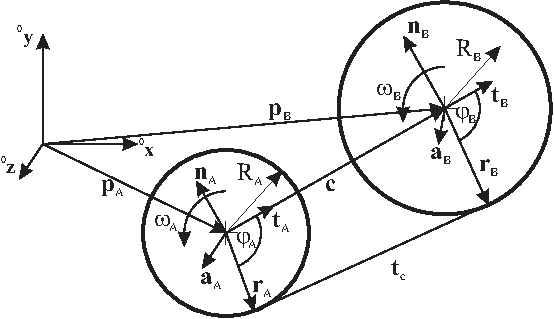
\includegraphics[width=10cm]{figures/CommonTangents3D.pdf}
      \end{center}
      \caption{Geometry of common tangent for two spatial circles defined by radii $R_A$ and $R_B$ as well as by the 
      normalized axis vectors $\av_A$ and $\av_B$. The tangent is undefined, if one of the axis vectors is parallel to the 
      vector $\cv$, which connects the two center points. The positive rotation sense is indicated by means of the 
      angular velocities $\omega_A$ and $\omega_B$.}
        \label{fig:ReevingSystemSprings:tangents}
    \end{figure}
    }
    \onlyRST{
    .. _fig-reevingsystemsprings-tangents:
    .. figure:: docs/theDoc/figures/CommonTangents3D.png
       :width: 500

       Geometry of common tangent for two spatial circles defined by radii $R_A$ and $R_B$ as well as by the normalized axis vectors $\av_A$ and $\av_B$. The tangent is undefined, if one of the axis vectors is parallel to the vector $\cv$, which connects the two center points. The positive rotation sense is indicated by means of the angular velocities $\omega_A$ and $\omega_B$.
    }
    %++++++++++++++++++++++++
    \mysubsubsubsection{Common tangent of two circles in 3D}
    In order to compute the total length of the rope of the reeving system, the tangent of two arbitrary circles in space needs to be computed.
    Considering \fig{fig:ReevingSystemSprings:tangents}, the relations are based on the
    center points of the circles $\pv_A$ and $\pv_B$, the radii $R_A$ and $R_B$ as well as
    the axis vectors $\av_A$ and $\av_B$, the latter vectors also defining the side at which the tangent contacts.
    For the definition of the tangent, the vectors $\rv_A$ and $\rv_B$ need to be computed.
    
    For the special case of $R_A=R_B=0$, it follows that $\rv_A=\pv_A$ and $\rv_B=\pv_B$.
    Otherwise, we first compute the vector between circle centers,
    \be
      \cv = \pv_B - \pv_A, \quad \mathrm{and} \quad \cv_0 = \frac{\cv}{|\cv|} \eqComma
    \ee
    and obtain the tangent vectors
    \be
      \tv_A = \tv_B = \cv_0 \eqComma
    \ee
    as well as the normal vectors
    \be
      \nv_A = \av_A \times \cv_0, \quad \mathrm{and} \quad
      \nv_B = \av_B \times \cv_0 \eqDot
    \ee
    Note that the orientation of the axis vectors $\av_A$ and $\av_B$ defines the orientation of the normals.
    By definition, we assume the following conditions,
    \be
      \nv_A\tp \rv_A < 0, \quad \mathrm{and} \quad 
      \nv_B\tp \rv_B < 0 \eqDot
    \ee
    For two circles with equal radius and axes orientations, the angles result in $\varphi_A=\varphi_B=\pi$.
    In general, the unknown vectors $\rv_A$ and $\rv_B$ are computed by means of Newton's method.
    The unknown tangent vector is given as 
    \be
      \tv_c = \pv_B + \rv_B - \pv_A - \rv_A = \cv + \rv_B - \rv_A \eqDot
    \ee
    We now parameterize the two unknown vectors by means of unknown angles $\varphi_A$ and $\varphi_B$,
    \be
      \rv_A = -R_A \left( \cos(\varphi_A) \tv_A - \sin(\varphi_A) \nv_A \right),
      \quad \mathrm{and} \quad 
      \rv_B = -R_B \left( \cos(\varphi_B) \tv_B - \sin(\varphi_B) \nv_B \right) \eqDot
    \ee
    As vectors $\rv_A$ and $\rv_B$ must be perpendicular to $\tv_c$, it follows that
    \be
      \rv_A\tp (\cv + \rv_B - \rv_A) = 0,
      \quad \mathrm{and} \quad 
      \rv_B\tp (\cv + \rv_B - \rv_A) = 0,
    \ee
    or
    \be \label{eq:ReevingSystemSprings:Newton}
      \rv_A\tp \cv + \rv_A\tp \rv_B - R_A^2 = 0,
      \quad \mathrm{and} \quad 
      \rv_B\tp \cv - \rv_B\tp\rv_A + R_B^2 = 0 \eqDot
    \ee
    The relations \eq{eq:ReevingSystemSprings:Newton} reduce to only one equation, if either $R_A=0$ or $R_B = 0$.
    The equations can be solved by Newton's method by computing the jacobian of $\Jm_{CT}$ of \eq{eq:ReevingSystemSprings:Newton} w.r.t.\ the 
    unknown angles $\varphi_A$ and $\varphi_B$. The iterations are started with
    \be
      \varphi_A = \pi \quad \mathrm{and} \quad \varphi_B = \pi,
    \ee
    and iterate until the error is below a certain tolerance, for details see the implementation in \texttt{Geometry.h}.
    
    \mysubsubsubsection{Connector forces}
    The current rope length results from the configuration of sheaves, including start and end position:
    \be
      L = d_{m_0-m_1} + C_{m_1} + d_{m_1-m_2} + C_{m_2} + \ldots  + d_{m_{nr-2}-m_{nr-1}}
    \ee
    in which $d_{...}$ represents the free spans between two sheaves as computed from the common tangent in the previous section,
    and $C_{...}$ represents the length along the circumference of the according marker if the according radius $r$ is non-zero.
    The quantity $C_{...}$ can be computed easily as soon as the radius vectors to the tangents $\rv_A$ and $\rv_B$
    are known. Within a series of tangents, the previous to the current tangent will always enclose an angle between $0$ and $2\cdot \pi$.
    
    In case that \texttt{hasCoordinateMarkers=True}, the total reference length and its derivative result as
    \be
      L_0 = L_{ref} + f_0 \cdot q_{m_{c0}} + f_1 \cdot q_{m_{c1}}, \quad
      \dot L_0 = f_0 \cdot \dot q_{m_{c0}} + f_1 \cdot \dot q_{m_{c1}}, \quad
    \ee
    while we set $L_0 = L_{ref}$ and $\dot L_0=0$ otherwise.
    The linear force in the reeving system (assumed to be constant all over the rope) is computed as
    \be
      F_{lin} = (L-L_{0}) \frac{EA}{L_0} + (\dot L - \dot L_0)\frac{DA}{L_0}
    \ee
    The rope force is computed from
    \be
      F =   \begin{cases} F_{lin} \quad \mathrm{if} \quad F_{lin} > 0 \\
                          F_{reg} \cdot \mathrm{tanh}(F_{lin}/F_{reg})\quad \mathrm{else} 
            \end{cases}
    \ee
    Which allows small compressive forces $F_{reg}$.
    In case that $F_{reg} < 0$, compressive forces are not regularized (linear spring).
    The case $F_{reg} = 0$ will be used in future only in combination with a data node, 
    which allows switching similar as in friction and contact elements.
    
    Note that in case of $L_0=0$, the term $\frac{1}{L_0}$ is replaced by $1000$.
    However, this case must be avoided by the user by choosing appropriate parameters for the system.

    Additional damping may be added via the parameters $DT$ and $DS$, which have to be treated carefully. The shearing parameter may
    be helpful to damp undesired oscillatory shearing motion, however, it may also damp rigid body motion of the overall mechanism.

    Further details are given in the implementation and examples are provided in the \texttt{Examples} and \texttt{TestModels} folders.
    %%RSTCOMPATIBLE
\vspace{6pt}\par\noindent\rule{\textwidth}{0.4pt}
%
\noindent For examples on ObjectConnectorReevingSystemSprings see Relevant Examples and TestModels with weblink:
\bi
\item \exuUrl{https://github.com/jgerstmayr/EXUDYN/blob/master/main/pythonDev/Examples/craneReevingSystem.py}{\texttt{craneReevingSystem.py}} (Examples/)
\item \exuUrl{https://github.com/jgerstmayr/EXUDYN/blob/master/main/pythonDev/TestModels/reevingSystemSpringsTest.py}{\texttt{reevingSystemSpringsTest.py}} (TestModels/)

\ei

%
\newpage

%+++++++++++++++++++++++++++++++++++

\mysubsubsection{ObjectConnectorRollingDiscPenalty}
\label{sec:item:ObjectConnectorRollingDiscPenalty}
A (flexible) connector representing a rolling rigid disc (marker 1) on a flat surface (marker 0, ground body, not moving) in global $x$-$y$ plane. The connector is based on a penalty formulation and adds friction and slipping. The contraints works for discs as long as the disc axis and the plane normal vector are not parallel. Parameters may need to be adjusted for better convergence (e.g., dryFrictionProportionalZone). The formulation for the arbitrary disc axis is still under development and needs further testing. Note that the rolling body must have the reference point at the center of the disc.
\vspace{12pt}\\

\noindent \mybold{Additional information for ObjectConnectorRollingDiscPenalty}:
\bi
  \item This \texttt{Object} has/provides the following types = \texttt{Connector}
  \item Requested \texttt{Marker} type = \texttt{Position} + \texttt{Orientation}
  \item Requested \texttt{Node} type = \texttt{GenericData}
  \item {\bf Short name} for Python = \texttt{RollingDiscPenalty}
  \item {\bf Short name} for Python visualization object = \texttt{VRollingDiscPenalty}
\ei\vspace{12pt} \noindent 
The item \mybold{ObjectConnectorRollingDiscPenalty} with type = 'ConnectorRollingDiscPenalty' has the following parameters:
\vspace{-0.5cm}\\
\vspace{-0.5cm}\\
%reference manual TABLE
\begin{center}
  \footnotesize
  \begin{longtable}{| p{4.5cm} | p{2.5cm} | p{0.5cm} | p{2.5cm} | p{6cm} |}
    \hline
    \bf Name & \bf type & \bf size & \bf default value & \bf description \\ \hline
    name &     String &      &     '' &     constraints's unique name\\ \hline
    markerNumbers &     ArrayMarkerIndex &     \tabnewline 2 &     [ invalid [-1], invalid [-1] ] &     \tabnewline list of markers used in connector; $m0$ represents a point at the plane surface (normal of surface plane defined by planeNormal); the ground can also be a moving rigid body; $m1$ represents the rolling body, which has its reference point (=local position [0,0,0]) at the disc center point\\ \hline
    nodeNumber &     NodeIndex &      &     invalid (-1) &     \tabnewline node number of a NodeGenericData (size=3) for 3 dataCoordinates, needed for discontinuous iteration (friction and contact)\\ \hline
    discRadius &     PReal &      &     0. &     defines the disc radius\\ \hline
    discAxis &     Vector3D &      &     [1,0,0] &     axis of disc defined in marker $m1$ frame\\ \hline
    planeNormal &     Vector3D &      &     [0,0,1] &     normal to the contact / rolling plane (ground); note that the plane reference point can be arbitrarily chosen by the location of the marker $m0$\\ \hline
    dryFrictionAngle &     Real &      &     0. &     angle [SI:1 (rad)] which defines a rotation of the local tangential coordinates dry friction; this allows to model Mecanum wheels with specified roll angle\\ \hline
    contactStiffness &     UReal &      &     0. &     normal contact stiffness [SI:N/m]\\ \hline
    contactDamping &     UReal &      &     0. &     normal contact damping [SI:N/(m s)]\\ \hline
    dryFriction &     Vector2D &      &     [0,0] &     dry friction coefficients [SI:1] in local marker 1 joint $J1$ coordinates; if $\alpha_t==0$, lateral direction $l=x$ and forward direction $f=y$; assuming a normal force $f_n$, the local friction force can be computed as $\LU{J1}{\vp{f_{t,x}}{f_{t,y}}} = \vp{\mu_x f_n}{\mu_y f_n}$\\ \hline
    dryFrictionProportionalZone &     Real &      &     0. &     limit velocity [m/s] up to which the friction is proportional to velocity (for regularization / avoid numerical oscillations)\\ \hline
    viscousFriction &     Vector2D &      &     [0,0] &     viscous friction coefficients [SI:1/(m/s)] in local marker 1 joint $J1$ coordinates; proportional to slipping velocity, leading to increasing slipping friction force for increasing slipping velocity\\ \hline
    rollingFrictionViscous &     Real &      &     0. &     rolling friction [SI:1], which acts against the velocity of the trail on ground and leads to a force proportional to the contact normal force; currently, only implemented for disc axis parallel to ground!\\ \hline
    useLinearProportionalZone &     Bool &      &     False &     if True, a linear proportional zone is used; the linear zone performs better in implicit time integration as the Jacobian has a constant tangent in the sticking case\\ \hline
    activeConnector &     Bool &      &     True &     flag, which determines, if the connector is active; used to deactivate (temporarily) a connector or constraint\\ \hline
    visualization &     VObjectConnectorRollingDiscPenalty &      &      &     parameters for visualization of item\\ \hline
\end{longtable}
\end{center}

\noindent The item VObjectConnectorRollingDiscPenalty has the following parameters:
%reference manual TABLE
\begin{center}
  \footnotesize
  \begin{longtable}{| p{4.5cm} | p{2.5cm} | p{0.5cm} | p{2.5cm} | p{6cm} |}
    \hline
    \bf Name & \bf type & \bf size & \bf default value & \bf description \\ \hline
    show &     Bool &      &     True &     set true, if item is shown in visualization and false if it is not shown\\ \hline
    discWidth &     float &      &     0.1 &     width of disc for drawing\\ \hline
    color &     Float4 &      &     [-1.,-1.,-1.,-1.] &     \tabnewline RGBA connector color; if R==-1, use default color\\ \hline
\end{longtable}
\end{center}
\par\noindent\rule{\textwidth}{0.4pt}
\mysubsubsubsection{DESCRIPTION of ObjectConnectorRollingDiscPenalty:}
\label{description_ObjectConnectorRollingDiscPenalty}
\paragraph{Information on input parameters:} 
\startTable{input parameter}{symbol}{description see tables above}
\rowTable{markerNumbers}{$[m0,m1]\tp$}{}
\rowTable{nodeNumber}{$n_d$}{}
\rowTable{discAxis}{$\LU{m1}{\wv_{1}}, \;\; |\LU{m1}{\wv_{1}}| = 1$}{}
\rowTable{planeNormal}{$\LU{m0}{\vv_{PN}}, \;\; |\LU{m0}{\vv_{PN}}| = 1$}{}
\rowTable{dryFrictionAngle}{$\alpha_t$}{}
\rowTable{contactStiffness}{$k_c$}{}
\rowTable{contactDamping}{$d_c$}{}
\rowTable{dryFriction}{$[\mu_x,\mu_y]\tp$}{}
\rowTable{dryFrictionProportionalZone}{$v_\mu$}{}
\rowTable{viscousFriction}{$[d_x, d_y]\tp$}{}
\rowTable{rollingFrictionViscous}{$\mu_r$}{}
\finishTable

\mybold{The following output variables are available as OutputVariableType in sensors, Get...Output() and other functions}:
\begin{center}
\footnotesize
\begin{longtable}{| p{5cm} | p{5cm} | p{6cm} |} 
\hline
\bf output variable & \bf symbol & \bf description \\ \hline
Position & $\LU{0}{\pv}_{G}$ & current global position of contact point between rolling disc and ground\\ \hline
Velocity & $\LU{0}{\vv}_{trail}$ & current velocity of the trail (according to motion of the contact point along the trail!) in global coordinates; this is not the velocity of the contact point!\\ \hline
VelocityLocal & $\LU{J1}{\vv}$ & relative slip velocity at contact point in special $J1$ joint coordinates\\ \hline
ForceLocal & $\LU{J1}{\fv} = \LU{0}{[f_{t,x},\, f_{t,y},\, f_{n}]\tp}$ & contact forces acting on disc, in special $J1$ joint coordinates, see section Connector Forces, $f_{t,x}$ being the lateral force (parallel to ground plane), $f_{t,y}$ being the longitudinal force and $f_{n}$ being the contact normal force\\ \hline
RotationMatrix & $\LU{0,J1}{\Am} = [\LU{0}{\wv_{lat}},\, \LU{0}{\wv}_2,\, \LU{0}{\vv_{PN}}]$ & transformation matrix of special joint coordinates $J1$ to global coordinates\\ \hline
\end{longtable}
\end{center}
 \noindent
    \mysubsubsubsection{Definition of quantities}
    \startTable{intermediate variables}{symbol}{description}
    \rowTable{marker m0 position}{$\LU{0}{\pv}_{m0}$}{current global position which is provided by marker m0, any ground reference point; currently unused}
    \rowTable{marker m0 orientation}{$\LU{0,m0}{\Rot}$}{current rotation matrix provided by marker m0; currently unused}
    \rowTable{marker m1 position}{$\LU{0}{\pv}_{m1}$}{center of disc}
    \rowTable{marker m1 orientation}{$\LU{0,m1}{\Rot}$}{current rotation matrix provided by marker m1}
    \rowTable{data coordinates}{$\xv=[x_0,\,x_1,\,x_2]\tp$}{data coordinates for $[x_0,\,x_1]$: hold the sliding velocity in lateral and longitudinal direction of last discontinuous iteration; $x_2$: represents gap of last discontinuous iteration (in contact normal direction)}
    %
    %\rowTable{marker m0 velocity}{$\LU{0}{\vv}_{m0}$}{current global velocity which is provided by marker m0}
    \rowTable{marker m1 velocity}{$\LU{0}{\vv}_{m1}$}{accordingly}
    %\rowTable{marker m0 angular velocity}{$\LU{0}{\tomega}_{m0}$}{current angular velocity vector provided by marker m0}
    \rowTable{marker m1 angular velocity}{$\LU{0}{\tomega}_{m1}$}{current angular velocity vector provided by marker m1}
    %
    \rowTable{ground normal vector}{$\LU{0}{\vv_{PN}} = \LU{0,m0}{\Am} \LU{m0}{\vv_{PN}}$}{normalized normal vector to the ground body (rotates with marker $m0$ if not fixed to ground)}
    \rowTable{ground position B}{$\LU{0}{\pv}_{B}$}{disc center point projected on ground (normal projection)}
    \rowTable{ground position C}{$\LU{0}{\pv}_{C}$}{contact point of disc with ground}
    \rowTable{ground velocity C}{$\LU{0}{\vv}_{C}$}{velocity of disc at ground contact point (must be zero at end of iteration)}
    \rowTable{wheel axis vector}{$\LU{0}{\wv_1} =\LU{0,m1}{\Rot} \LU{m1}{\wv_{1}} $}{normalized disc axis vector in global coordinates}
    \rowTable{longitudinal vector}{$\LU{0}{\wv_2}$}{vector in longitudinal (motion) direction}
    \rowTable{contact point vector}{$\LU{0}{\wv_3}$}{normalized vector from disc center point in direction of contact point C}
    \rowTable{lateral vector}{$\LU{0}{\wv_{lat}} = \LU{0}{\vv_{PN}} \times \LU{0}{\wv}_2$}{vector in lateral direction, parallel to ground plane}
    \rowTable{$D1$ transformation matrix}{$\LU{0,D1}{\Am} = [\LU{0}{\wv_1},\, \LU{0}{\wv_2},\, \LU{0}{\wv_3}]$}{transformation of special disc coordinates $D1$ to global coordinates}
    %
    \rowTable{connector forces}{$\LU{J1}{\fv}=[f_{t,x},\,f_{t,y},\,f_n]\tp$}{joint force vector at contact point in joint 1 coordinates: x=lateral direction, y=longitudinal direction, z=plane normal (contact normal)}
    \finishTable
    
    \mysubsubsubsection{Geometric relations}
    %++++++++++++++++++++++++++++++++++++++++++++++++++++++++++
    \noindent The main geometrical setup is shown in the following figure:
    \ignoreRST{
    \begin{center}
        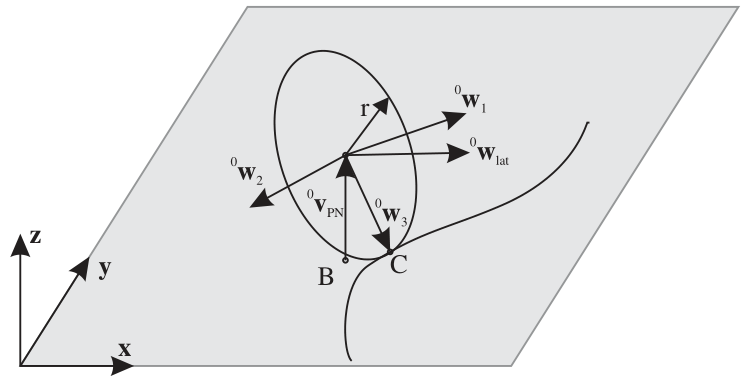
\includegraphics[height=4cm]{figures/ObjectJointRollingDiscSketch.pdf}
    \end{center}
    }
    \onlyRST{
    .. image:: docs/theDoc/figures/ObjectJointRollingDiscSketch.png
       :width: 600

    }
    First, the contact point $\LU{0}{\pv}_{C}$ must be computed.
    With the helper vector,
    \be
      \LU{0}{\xv} = \LU{0}{\wv}_1 \times \LU{0}{\vv_{PN}}
    \ee
    we create a disc coordinate system $D1$ ($\LU{0}{\wv}_1, \; \LU{0}{\wv}_2, \; \LU{0}{\wv}_3$), with the longitudinal direction,
    \be
      \LU{0}{\wv}_2 = \frac{1}{|\LU{0}{\xv}|} \LU{0}{\xv} 
    \ee
    and the vector to the contact point,
    \be
      \LU{0}{\wv}_3 = \LU{0}{\wv}_1 \times \LU{0}{\wv}_2
    \ee
    The vector from marker $m0$ position to the contact point can be computed from
    \be
      \LU{0}{\pv}_{C} = \LU{0}{\pv}_{m1} + r \cdot \LU{0}{\wv}_3 - \LU{0}{\pv}_{m0}
    \ee
    The velocity of the contact point at the disc is computed from,
    \be
      \LU{0}{\vv}_{C} = \LU{0}{\vv}_{m1} + \LU{0}{\tomega}_{m1} \times (r\cdot \LU{0}{\wv}_3)
                        - \left(\LU{0}{\vv}_{m0} + \LU{0}{\tomega}_{m0} \times \LU{0}{\pv}_{C} \right)
    \ee
    A second coordinate system, denoted as $J1$, is defined by vectors ($\LU{0}{\wv}_{lat}, \; \LU{0}{\wv}_2, \;  \LU{0}{\vv}_{PN}$), using
    \be
        \LU{0}{\wv}_{lat} = \LU{0}{\vv_{PN}} \times \LU{0}{\wv}_2
    \ee
    Note that {\bf in the case that} the rolling axis $\LU{0}{\wv}_1$ lies in the rolling plane, we obtain the special case
    $\LU{0}{\wv}_{lat} = \LU{0}{\wv}_1$ and $\LU{0}{\wv}_3 = -\LU{0}{\vv}_{PN}$.
                                                                     
    \mysubsubsubsection{Computation of normal and tangential forces}
    The connector forces at the contact point $C$ are computed as follows. 
    The normal contact force reads
    \be
      f_n = \left(k_c \cdot \LU{0}{\pv}_{C} + d_c \cdot \LU{0}{\vv}_{C} \right)\tp \LU{0}{\vv_{PN}} \eqDot
    \ee
    Note that due to the projection onto $\LU{0}{\vv_{PN}}$, this equation also works for inclined planes
    and reference points, that are not at $[0,0,0]\tp$.
    %
    The inplane velocity in joint coordinates,
    \be
      \LU{J1}{\vv_t} = [\LU{0}{\vv}_{C}\tp \LU{0}{\wv}_{lat}, \; \LU{0}{\vv}_{C}\tp \LU{0}{\wv}_2 ]\tp \eqComma
    \ee
    is used for the computation of tangential forces,
    \be
      \LU{J1}{\fv_t} = [f_{t,x} ,\; f_{t,y}]\tp = \LU{J1}{\tmu} \cdot \left( \phi(|\vv_t|,v_\mu) \cdot f_n \cdot \LU{J1}{\ev_t} \right) \eqComma
    \ee
    with the regularization function, see Geradin and Cardona \cite{GeradinCardona2001} (Sec.\ 7.9.3), if \texttt{useLinearProportionalZone=False},
    \be
      \phi(v, v_\mu) = 
        \left\{ 
            \begin{array}{ccl}
                \displaystyle \left( 2-\frac{v}{v_\mu} \right)\frac{v}{v_\mu} & \mathrm{if} & v \le v_\mu \\
                1 & \mathrm{if} & v > v_\mu \\
            \end{array}
            \right.
    \ee
    and the linear regularization function, if \texttt{useLinearProportionalZone=True},
    \be
      \phi(v, v_\mu) = 
        \left\{ 
            \begin{array}{ccl}
                \displaystyle \frac{v}{v_\mu} & \mathrm{if} & v \le v_\mu \\
                1 & \mathrm{if} & v > v_\mu \\
            \end{array}
            \right.
    \ee
    The direction of tangential slip is given as
    \be
      \LU{J1}{\ev_t} = 
        \left\{ 
            \begin{array}{ccl}
                \displaystyle \frac{\LU{J1}{\vv_t}}{|\vv_t|} &\mathrm{if}& |\vv_t|>0 \\
                %\left[0,\; 0\right]\tp &\mathrm{else}& \\
                \vp{0}{0} &\mathrm{else}& \\
            \end{array}
            \right.
    \ee
    The friction coefficient matrix $\LU{J1}{\tmu}$ is given in joint coordinates and computed from
    \be
      \LU{J1}{\tmu} = \mp{\mu_x + d_x \cdot |\vv_t|}{0}{0}{\mu_y + d_y \cdot |\vv_t|}
    \ee
    where for isotropic behaviour of surface and wheel, it will give a diagonal matrix with the friction coefficient in the diagonal.
    In case that the dry friction angle $\alpha_t$ is not zero, the $\tmu$ changes to
    \be
      \LU{J1}{\tmu} = \mp{\cos(\alpha_t)}{\sin(\alpha_t)}{-\sin(\alpha_t)}{\cos(\alpha_t)} 
      \mp{\mu_x + d_x \cdot |\vv_t|}{0}{0}{\mu_y + d_y \cdot |\vv_t|} 
      \mp{\cos(\alpha_t)}{-\sin(\alpha_t)}{\sin(\alpha_t)}{\cos(\alpha_t)}
    \ee
    %
    \mysubsubsubsection{Connector forces}
    Finally, the connector forces read in joint coordinates
    \be \label{eq:ConnectorRollingDiscPenalty:forces}
      \LU{J1}{\fv} = \vr{f_{t,x}}{f_{t,y}}{f_n}
    \ee
    and in global coordinates, they are computed from
    \be
      \LU{0}{\fv} = f_{t,x}\LU{0}{\wv}_{lat} + f_{t,y} \LU{0}{\wv}_2 + f_n \LU{0}{\vv}_{PN}
    \ee
    Due to the fact that the marker positions are not collocated with the contact point, 
    there are additional torques that need to be considered in the action on the body.
    The torque onto the disc (marker $m1$) is computed as
    \be
      \LU{0}{\ttau_{m1}} = (r\cdot \LU{0}{\wv}_3) \times \LU{0}{\fv}
    \ee
    The torque onto the ground (marker $m0$) is computed as
    \be
      \LU{0}{\ttau_{m0}} = \LU{0}{\pv}_{C} \times \LU{0}{\fv}
    \ee
    Note that if \texttt{activeConnector = False}, we replace \eq{eq:ConnectorRollingDiscPenalty:forces} with
    \be
      \LU{J1}{\fv} = \Null
    \ee
    %%RSTCOMPATIBLE
\vspace{6pt}\par\noindent\rule{\textwidth}{0.4pt}
%
\noindent For examples on ObjectConnectorRollingDiscPenalty see Relevant Examples and TestModels with weblink:
\bi
\item \exuUrl{https://github.com/jgerstmayr/EXUDYN/blob/master/main/pythonDev/Examples/bicycleIftommBenchmark.py}{\texttt{bicycleIftommBenchmark.py}} (Examples/)
\item \exuUrl{https://github.com/jgerstmayr/EXUDYN/blob/master/main/pythonDev/Examples/leggedRobot.py}{\texttt{leggedRobot.py}} (Examples/)
\item \exuUrl{https://github.com/jgerstmayr/EXUDYN/blob/master/main/pythonDev/Examples/mobileMecanumWheelRobotWithLidar.py}{\texttt{mobileMecanumWheelRobotWithLidar.py}} (Examples/)
\item \exuUrl{https://github.com/jgerstmayr/EXUDYN/blob/master/main/pythonDev/Examples/reinforcementLearningRobot.py}{\texttt{reinforcementLearningRobot.py}} (Examples/)
\item \exuUrl{https://github.com/jgerstmayr/EXUDYN/blob/master/main/pythonDev/TestModels/carRollingDiscTest.py}{\texttt{carRollingDiscTest.py}} (TestModels/)
\item \exuUrl{https://github.com/jgerstmayr/EXUDYN/blob/master/main/pythonDev/TestModels/laserScannerTest.py}{\texttt{laserScannerTest.py}} (TestModels/)
\item \exuUrl{https://github.com/jgerstmayr/EXUDYN/blob/master/main/pythonDev/TestModels/mecanumWheelRollingDiscTest.py}{\texttt{mecanumWheelRollingDiscTest.py}} (TestModels/)
\item \exuUrl{https://github.com/jgerstmayr/EXUDYN/blob/master/main/pythonDev/TestModels/rollingCoinPenaltyTest.py}{\texttt{rollingCoinPenaltyTest.py}} (TestModels/)
\item \exuUrl{https://github.com/jgerstmayr/EXUDYN/blob/master/main/pythonDev/TestModels/rollingDiscTangentialForces.py}{\texttt{rollingDiscTangentialForces.py}} (TestModels/)
\item \exuUrl{https://github.com/jgerstmayr/EXUDYN/blob/master/main/pythonDev/TestModels/rotatingTableTest.py}{\texttt{rotatingTableTest.py}} (TestModels/)

\ei

%
\newpage

%+++++++++++++++++++++++++++++++++++

\mysubsubsection{ObjectContactConvexRoll}
\label{sec:item:ObjectContactConvexRoll}
A contact connector representing a convex roll (marker 1) on a flat surface (marker 0, ground body, not moving) in global $x$-$y$ plane. The connector is similar to ObjectConnectorRollingDiscPenalty, but includes a (strictly) convex shape of the roll defined by a polynomial. It is based on a penalty formulation and adds friction and slipping. The formulation is still under development and needs further testing. Note that the rolling body must have the reference point at the center of the disc.
\vspace{12pt}\\

\noindent Author: Manzl Peter
\vspace{12pt}\\

\noindent \mybold{Additional information for ObjectContactConvexRoll}:
\bi
  \item This \texttt{Object} has/provides the following types = \texttt{Connector}
  \item Requested \texttt{Marker} type = \texttt{Position} + \texttt{Orientation}
  \item Requested \texttt{Node} type = \texttt{GenericData}
\ei\vspace{12pt} \noindent 
The item \mybold{ObjectContactConvexRoll} with type = 'ContactConvexRoll' has the following parameters:
\vspace{-0.5cm}\\
\vspace{-0.5cm}\\
%reference manual TABLE
\begin{center}
  \footnotesize
  \begin{longtable}{| p{4.5cm} | p{2.5cm} | p{0.5cm} | p{2.5cm} | p{6cm} |}
    \hline
    \bf Name & \bf type & \bf size & \bf default value & \bf description \\ \hline
    name &     String &      &     '' &     constraints's unique name\\ \hline
    markerNumbers &     ArrayMarkerIndex &     \tabnewline 2 &     [ invalid [-1], invalid [-1] ] &     \tabnewline list of markers used in connector; $m0$ represents the ground, which can undergo translations but not rotations, and $m1$ represents the rolling body, which has its reference point (=local position [0,0,0]) at the roll's center point\\ \hline
    nodeNumber &     NodeIndex &      &     invalid (-1) &     \tabnewline node number of a NodeGenericData (size=3) for 3 dataCoordinates, needed for discontinuous iteration (friction and contact)\\ \hline
    contactStiffness &     Real &      &     0. &     normal contact stiffness [SI:N/m]\\ \hline
    contactDamping &     Real &      &     0. &     normal contact damping [SI:N/(m s)]\\ \hline
    dynamicFriction &     UReal &      &     0. &     dynamic friction coefficient for friction model, see StribeckFunction in exudyn.physics, \refSection{sec:module:physics}\\ \hline
    staticFrictionOffset &     UReal &      &     0. &     static friction offset for friction model (static friction = dynamic friction + static offset), see StribeckFunction in exudyn.physics, \refSection{sec:module:physics}\\ \hline
    viscousFriction &     UReal &      &     0. &     viscous friction coefficient (velocity dependent part) for friction model, see StribeckFunction in exudyn.physics, \refSection{sec:module:physics}\\ \hline
    exponentialDecayStatic &     PReal &      &     1e-3 &     exponential decay of static friction offset (must not be zero!), see StribeckFunction in exudyn.physics (named expVel there!), \refSection{sec:module:physics}\\ \hline
    frictionProportionalZone &     UReal &      &     1e-3 &     limit velocity [m/s] up to which the friction is proportional to velocity (for regularization / avoid numerical oscillations), see StribeckFunction in exudyn.physics (named regVel there!), \refSection{sec:module:physics}\\ \hline
    rollLength &     UReal &      &     0. &     roll length [m], symmetric w.r.t.\ centerpoint\\ \hline
    coefficientsHull &     NumpyVector &      &      [] &     a vector of polynomial coefficients, which provides the polynomial of the CONVEX hull of the roll; $\mathrm{hull}(x) = k_0 x^{n_p-1} + k x^{n_p-2} + \ldots + k_{n_p-2} x  + k_{n_p-1}$\\ \hline
    coefficientsHullDerivative &     NumpyVector &      &     [] &     polynomial coefficients of the polynomial $\mathrm{hull}^\prime(x)$\\ \hline
    coefficientsHullDDerivative &     NumpyVector &      &     [] &     second derivative of the hull polynomial.\\ \hline
    rBoundingSphere &     UReal &      &     0 &     The  radius of the bounding sphere for the contact pre-check, calculated from the polynomial coefficients of the hull\\ \hline
    pContact &     Vector3D &      &     [0,0,0] &     The  current potential contact point. Contact occures if pContact[2] < 0. \\ \hline
    activeConnector &     Bool &      &     True &     flag, which determines, if the connector is active; used to deactivate (temporarily) a connector or constraint\\ \hline
    visualization &     VObjectContactConvexRoll &      &      &     parameters for visualization of item\\ \hline
\end{longtable}
\end{center}

\noindent The item VObjectContactConvexRoll has the following parameters:
%reference manual TABLE
\begin{center}
  \footnotesize
  \begin{longtable}{| p{4.5cm} | p{2.5cm} | p{0.5cm} | p{2.5cm} | p{6cm} |}
    \hline
    \bf Name & \bf type & \bf size & \bf default value & \bf description \\ \hline
    show &     Bool &      &     True &     set true, if item is shown in visualization and false if it is not shown\\ \hline
    color &     Float4 &      &     [-1.,-1.,-1.,-1.] &     \tabnewline RGBA connector color; if R==-1, use default color\\ \hline
\end{longtable}
\end{center}
\par\noindent\rule{\textwidth}{0.4pt}
\mysubsubsubsection{DESCRIPTION of ObjectContactConvexRoll:}
\label{description_ObjectContactConvexRoll}
\paragraph{Information on input parameters:} 
\startTable{input parameter}{symbol}{description see tables above}
\rowTable{markerNumbers}{$[m0,m1]\tp$}{}
\rowTable{nodeNumber}{$n_d$}{}
\rowTable{contactStiffness}{$k_c$}{}
\rowTable{contactDamping}{$d_c$}{}
\rowTable{dynamicFriction}{$\mu_d$}{}
\rowTable{staticFrictionOffset}{$\mu_{s_off}$}{}
\rowTable{viscousFriction}{$\mu_v$}{}
\rowTable{exponentialDecayStatic}{$v_{exp}$}{}
\rowTable{frictionProportionalZone}{$v_{reg}$}{}
\rowTable{rollLength}{$L$}{}
\rowTable{coefficientsHull}{$\kv \in \Rcal^{n_p}$}{}
\rowTable{coefficientsHullDerivative}{$\kv^\prime \in \Rcal^{n_p}$}{}
\finishTable

\mybold{The following output variables are available as OutputVariableType in sensors, Get...Output() and other functions}:
\begin{center}
\footnotesize
\begin{longtable}{| p{5cm} | p{5cm} | p{6cm} |} 
\hline
\bf output variable & \bf symbol & \bf description \\ \hline
Position & $\LU{0}{\pv}_{C}$ & current global position of contact point between roller and ground\\ \hline
Velocity & $\LU{0}{\vv}_{C}$ & current velocity of the trail (contact) point in global coordinates; this is the velocity with which the contact moves over the ground plane\\ \hline
Force & $\LU{0}{\fv}$ & Roll-ground force in ground coordinates\\ \hline
Torque & $\LU{0}{\mv}$ & Roll-ground torque in ground coordinates\\ \hline
\end{longtable}
\end{center}
 \noindent
    \mysubsubsubsection{Definition of quantities}
    \startTable{intermediate variables}{symbol}{description}
    \rowTable{marker m0 position}{$\LU{0}{\pv}_{m0}$}{current global position which is provided by marker m0, any ground reference point; currently unused}
    \rowTable{marker m0 orientation}{$\LU{0,m0}{\Rot}$}{current rotation matrix provided by marker m0; currently unused}
    \rowTable{marker m1 position}{$\LU{0}{\pv}_{m1}$}{center of roll}
    \rowTable{Contact position}{$\LU{0}{\pv}_{C}$}{Position of the Contact point C in the global frame 0}
    \rowTable{Position marker m1 to contact}{$\LU{0}{\pv}_{\mathrm{m1, C}}$}{Position of the contact point C relative to the marker m1 in global frame}
    \rowTable{marker m1 orientation}{$\LU{0,m1}{\Rot}$}{current rotation matrix provided by marker m1}
    \rowTable{data coordinates}{$\xv=[x_0,\,x_1,\,x_2]\tp$}{data coordinates for $[x_0,\,x_1]$: hold the sliding velocity in lateral and longitudinal direction of last discontinuous iteration; $x_2$: represents gap of last discontinuous iteration (in contact normal direction)}
    %
    %\rowTable{marker m0 velocity}{$\LU{0}{\vv}_{m0}$}{current global velocity which is provided by marker m0}
    \rowTable{marker m1 velocity}{$\LU{0}{\vv}_{m1}$}{current global velocity which is provided by marker m1}
    %\rowTable{marker m0 angular velocity}{$\LU{0}{\tomega}_{m0}$}{current angular velocity vector provided by marker m0}
    \rowTable{marker m1 angular velocity}{$\LU{0}{\tomega}_{m1}$}{current angular velocity vector provided by marker m1}
    %
    \rowTable{ground normal vector}{$\LU{0}{\nv}$}{normalized normal vector to the (moving, but not rotating) ground, by default [0,0,1]}
    
    %    \rowTable{ground position B}{$\LU{0}{\pv}_{B}$}{roll center point projected on ground (normal projection)}
    %    \rowTable{ground position C}{$\LU{0}{\pv}_{C}$}{contact point of disc with ground}
    %    \rowTable{ground velocity C}{$\LU{0}{\vv}_{C}$}{velocity of disc at ground contact point (must be zero at end of iteration)}
    %    \rowTable{wheel axis vector}{$\LU{0}{\wv}_1 =\LU{0,m1}{\Rot} \cdot [1,0,0]\tp $}{normalized disc axis vector, currently $[1,0,0]\tp$ in local coordinates}
    %    \rowTable{longitudinal vector}{$\LU{0}{\wv}_2$}{vector in longitudinal (motion) direction}
    %    \rowTable{lateral vector}{$\LU{0}{\wv}_l = \LU{0}{\vv_{PN}} \times \LU{0}{\wv}_2 = [-\wv_{2,y}, \wv_{2,x}, 0]$}{vector in lateral direction, lies in ground plane}
    %    \rowTable{contact point vector}{$\LU{0}{\wv}_3$}{normalized vector from disc center point in direction of contact point C}
    %
    %    \rowTable{connector forces}{$\LU{J1}{\fv}=[f_{t,x},\,f_{t,y},\,f_n]\tp$}{joint force vector at contact point in joint 1 coordinates: x=lateral direction, y=longitudinal direction, z=plane normal (contact normal)}
    \finishTable
    %
    \mysubsubsubsection{Geometric relations}
    %++++++++++++++++++++++++++++++++++++++++++++++++++++++++++
    The geometrical setup is shown in \fig{fig:ObjectContactConvexRoll:sketch}. To calculate the contact point of the convex body of revolution the contact (ground) plane is rotated into the local frame of the body. In this local frame in which the generatrix of the body of revolution is described by the polynomial function
    \be
    \mathrm{r}(^bx) = \sum_{i=0}^n k_i \; x^{n-i} \label{eq:ConnectorConvexRolling:polynomial}
    \ee
    with the coefficients of the hull $a_i$. As a pre-Check for the contact two spheres are put into both ends of the object with the maximum radius and only if one of these is in contact. The contact point $^{\mathrm{b}}\pv_{\mathrm{m1,C}} $ is calculated relative to the bodies marker \texttt{m1} in the bodies local frame and transformed accordingly. 
    The contact point C can for be calculated convex bodies by matching the derivative of the polynomial $r(^bx)$ with the gradient of the contact plane, shown in \fig{fig:ObjectContactConvexRoll:sketch}, explained in detail in \cite{ManzlGerstmayr2021}. 
    At the contact point a normal force $\fv_{\mathrm{N}} = [ 0 \; 0 \; \mathrm{f}_{\mathrm{N}} ]\tp$  with 
    \be
    \mathrm{f}_{\mathrm{N}} = \begin{cases}
    - (k_c \, z_{\mathrm{pen}} + d_c \,  \dot{z}_{\mathrm{pen}})  &\text{$z_{\mathrm{pen}}>0$} \\ % darstellen dämpfung 
    0 &\text{else} \label{eq_FpenContact}
    \end{cases}
    \ee
    acts against the penetration of the ground. The penetration depth $z_{\mathrm{pen}}$ is the z-component of the position vector of the contact point relative to the ground frame ${^0\pv_{\mathrm{C}}}$. 
    \ignoreRST{
    \begin{figure}[tbph]
    \begin{center}
            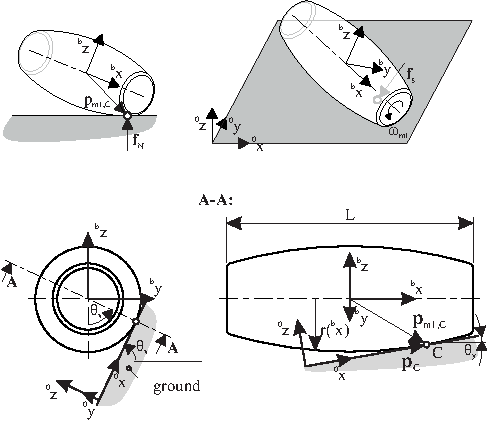
\includegraphics[width=10cm]{figures/ConvexRolling.pdf}
            \caption{Sketch of the roller Dimensions. The rollers radius $r({^bx})$ is described by the polynomial \texttt{coefficientsHull}.}
            \label{fig:ObjectContactConvexRoll:sketch}
    \end{center}
    \end{figure}
    }
    \onlyRST{
    .. _fig-objectcontactconvexroll-sketch:
    .. figure:: docs/theDoc/figures/ConvexRolling.png
       :width: 600

       Sketch of the roller Dimensions. The rollers radius $r({^bx})$ is described by the polynomial \texttt{coefficientsHull}.
    }

    \noindent
    The revolution results in a velocity of 
    \be
    ^{0}\vv_{C} ={^{0}{\tomega_{\mathrm{m1}}}} \times {^{0}{\pv_{\mathrm{m1,\,C}}}}
    \ee
    in the contact point, while the tangential component of the velocity of the body itself with the normal Vector to the contact plane $\nv$ follows to
    \be 
    \LURU{0}{\vv}{\mathrm{m1,\,t}}{} = \LU{0}{\vv_{\mathrm{m1}}} - {^0\nv} \, \left({^0\nv}^T \, \LU{0}{\vv_{\mathrm{m1}}}\right).
    \ee 
    Therefore the slip velocity of the body can be calculated with
    \be
    \LURU{0}{\vv}{\mathrm{s}}{} = \LURU{0}{\vv}{C}{} - {^0\vv_{\mathrm{m1,\,t}}}
    \ee
    and points in the direction 
    \be
    \LURU{0}{\rv}{s}{} = \frac{1}{\left\lVert \LURU{0}{\vv}{\mathrm{s}}{}\right\rVert} {^0{\vv}_{\mathrm{s}}}.
    \ee
    \noindent The slip force is then calculated
    \be
      ^0\fv_{\mathrm{s}} = \mu(\left\lVert\LU{}{^0\vv_{\mathrm{s}}}\right\rVert)  \, \mathrm{f}_{\mathrm{N}} \, {^0\rv_\mathrm{s}}
    \ee
    and uses for the friction coefficient $\mu$ the regularized friction approach from the StribeckFunction, see \refSection{sec:module:physics}. 
    The torque 
    \be
      ^0\ttau = {^0\pv_{\mathrm{m1,\,C}}} \times (^0\fv_{\mathrm{N}} + {^0\fv_{\mathrm{s}}})
    \ee
    acts onto the body, resulting from the slip force acting not in the bodies center. 
    %%RSTCOMPATIBLE
\vspace{6pt}\par\noindent\rule{\textwidth}{0.4pt}
%
\noindent For examples on ObjectContactConvexRoll see Relevant Examples and TestModels with weblink:
\bi
\item \exuUrl{https://github.com/jgerstmayr/EXUDYN/blob/master/main/pythonDev/TestModels/ConvexContactTest.py}{\texttt{ConvexContactTest.py}} (TestModels/)

\ei

%
\newpage

%+++++++++++++++++++++++++++++++++++

\mysubsubsection{ObjectContactCoordinate}
\label{sec:item:ObjectContactCoordinate}
A penalty-based contact condition for one coordinate; the contact gap $g$ is defined as $g=marker.value[1]- marker.value[0] - offset$; the contact force $f_c$ is zero for $gap>0$ and otherwise computed from $f_c = g*contactStiffness + \dot g*contactDamping$; during Newton iterations, the contact force is actived only, if $dataCoordinate[0] <= 0$; dataCoordinate is set equal to gap in nonlinear iterations, but not modified in Newton iterations.
\vspace{12pt}\\

\noindent \mybold{Additional information for ObjectContactCoordinate}:
\bi
  \item This \texttt{Object} has/provides the following types = \texttt{Connector}
  \item Requested \texttt{Marker} type = \texttt{Coordinate}
  \item Requested \texttt{Node} type = \texttt{GenericData}
\ei\vspace{12pt} \noindent 
The item \mybold{ObjectContactCoordinate} with type = 'ContactCoordinate' has the following parameters:
\vspace{-0.5cm}\\
\vspace{-0.5cm}\\
%reference manual TABLE
\begin{center}
  \footnotesize
  \begin{longtable}{| p{4.5cm} | p{2.5cm} | p{0.5cm} | p{2.5cm} | p{6cm} |}
    \hline
    \bf Name & \bf type & \bf size & \bf default value & \bf description \\ \hline
    name &     String &      &     '' &     connector's unique name\\ \hline
    markerNumbers &     ArrayMarkerIndex &     \tabnewline  &     [ invalid [-1], invalid [-1] ] &     \tabnewline markers define contact gap\\ \hline
    nodeNumber &     NodeIndex &      &     invalid (-1) &     \tabnewline node number of a NodeGenericData for 1 dataCoordinate (used for active set strategy ==> holds the gap of the last discontinuous iteration)\\ \hline
    contactStiffness &     UReal &      &     0. &     contact (penalty) stiffness [SI:N/m]; acts only upon penetration\\ \hline
    contactDamping &     UReal &      &     0. &     contact damping [SI:N/(m s)]; acts only upon penetration\\ \hline
    offset &     Real &      &     0. &     offset [SI:m] of contact\\ \hline
    activeConnector &     Bool &      &     True &     flag, which determines, if the connector is active; used to deactivate (temporarily) a connector or constraint\\ \hline
    visualization &     VObjectContactCoordinate &      &      &     parameters for visualization of item\\ \hline
\end{longtable}
\end{center}

\noindent The item VObjectContactCoordinate has the following parameters:
%reference manual TABLE
\begin{center}
  \footnotesize
  \begin{longtable}{| p{4.5cm} | p{2.5cm} | p{0.5cm} | p{2.5cm} | p{6cm} |}
    \hline
    \bf Name & \bf type & \bf size & \bf default value & \bf description \\ \hline
    show &     Bool &      &     True &     set true, if item is shown in visualization and false if it is not shown\\ \hline
    drawSize &     float &      &     -1. &     drawing size = diameter of spring; size == -1.f means that default connector size is used\\ \hline
    color &     Float4 &      &     [-1.,-1.,-1.,-1.] &     \tabnewline RGBA connector color; if R==-1, use default color\\ \hline
\end{longtable}
\end{center}
\par\noindent\rule{\textwidth}{0.4pt}
\mysubsubsubsection{DESCRIPTION of ObjectContactCoordinate:}
\label{description_ObjectContactCoordinate}
\vspace{6pt}\par\noindent\rule{\textwidth}{0.4pt}
%
\noindent For examples on ObjectContactCoordinate see Relevant Examples and TestModels with weblink:
\bi
\item \exuUrl{https://github.com/jgerstmayr/EXUDYN/blob/master/main/pythonDev/Examples/ANCFcontactCircle.py}{\texttt{ANCFcontactCircle.py}} (Examples/)
\item \exuUrl{https://github.com/jgerstmayr/EXUDYN/blob/master/main/pythonDev/Examples/ANCFcontactCircle2.py}{\texttt{ANCFcontactCircle2.py}} (Examples/)
\item \exuUrl{https://github.com/jgerstmayr/EXUDYN/blob/master/main/pythonDev/TestModels/ANCFcontactCircleTest.py}{\texttt{ANCFcontactCircleTest.py}} (TestModels/)
\item \exuUrl{https://github.com/jgerstmayr/EXUDYN/blob/master/main/pythonDev/TestModels/contactCoordinateTest.py}{\texttt{contactCoordinateTest.py}} (TestModels/)

\ei

%
\newpage

%+++++++++++++++++++++++++++++++++++

\mysubsubsection{ObjectContactCircleCable2D}
\label{sec:item:ObjectContactCircleCable2D}
A very specialized penalty-based contact condition between a 2D circle (=marker0, any Position-marker) on a body and an ANCFCable2DShape (=marker1, Marker: BodyCable2DShape), in xy-plane; a node NodeGenericData is required with the number of cordinates according to the number of contact segments; the contact gap $g$ is integrated (piecewise linear) along the cable and circle; the contact force $f_c$ is zero for $gap>0$ and otherwise computed from $f_c = g*contactStiffness + \dot g*contactDamping$; during Newton iterations, the contact force is actived only, if $dataCoordinate[0] <= 0$; dataCoordinate is set equal to gap in nonlinear iterations, but not modified in Newton iterations.
\vspace{12pt}\\

\noindent \mybold{Additional information for ObjectContactCircleCable2D}:
\bi
  \item This \texttt{Object} has/provides the following types = \texttt{Connector}
  \item Requested \texttt{Marker} type = \texttt{\_None}
  \item Requested \texttt{Node} type = \texttt{GenericData}
\ei\vspace{12pt} \noindent 
The item \mybold{ObjectContactCircleCable2D} with type = 'ContactCircleCable2D' has the following parameters:
\vspace{-0.5cm}\\
\vspace{-0.5cm}\\
%reference manual TABLE
\begin{center}
  \footnotesize
  \begin{longtable}{| p{4.5cm} | p{2.5cm} | p{0.5cm} | p{2.5cm} | p{6cm} |}
    \hline
    \bf Name & \bf type & \bf size & \bf default value & \bf description \\ \hline
    name &     String &      &     '' &     connector's unique name\\ \hline
    markerNumbers &     ArrayMarkerIndex &     \tabnewline  &     [ invalid [-1], invalid [-1] ] &     \tabnewline markers define contact gap\\ \hline
    nodeNumber &     NodeIndex &      &     invalid (-1) &     \tabnewline node number of a NodeGenericData for nSegments dataCoordinates (used for active set strategy ==> hold the gap of the last discontinuous iteration and the friction state)\\ \hline
    numberOfContactSegments &     Index &      &     3 &     number of linear contact segments to determine contact; each segment is a line and is associated to a data (history) variable; must be same as in according marker\\ \hline
    contactStiffness &     UReal &      &     0. &     contact (penalty) stiffness [SI:N/m/(contact segment)]; the stiffness is per contact segment; specific contact forces (per length) $f_N$ act in contact normal direction only upon penetration\\ \hline
    contactDamping &     UReal &      &     0. &     contact damping [SI:N/(m s)/(contact segment)]; the damping is per contact segment; acts in contact normal direction only upon penetration\\ \hline
    circleRadius &     UReal &      &     0. &     radius [SI:m] of contact circle\\ \hline
    offset &     Real &      &     0. &     offset [SI:m] of contact, e.g. to include thickness of cable element\\ \hline
    activeConnector &     Bool &      &     True &     flag, which determines, if the connector is active; used to deactivate (temporarily) a connector or constraint\\ \hline
    visualization &     VObjectContactCircleCable2D &      &      &     parameters for visualization of item\\ \hline
\end{longtable}
\end{center}

\noindent The item VObjectContactCircleCable2D has the following parameters:
%reference manual TABLE
\begin{center}
  \footnotesize
  \begin{longtable}{| p{4.5cm} | p{2.5cm} | p{0.5cm} | p{2.5cm} | p{6cm} |}
    \hline
    \bf Name & \bf type & \bf size & \bf default value & \bf description \\ \hline
    show &     Bool &      &     True &     set true, if item is shown in visualization and false if it is not shown\\ \hline
    showContactCircle &     Bool &      &     True &     if True and show=True, the underlying contact circle is shown; uses circleTiling*4 for tiling (from VisualizationSettings.general)\\ \hline
    drawSize &     float &      &     -1. &     drawing size = diameter of spring; size == -1.f means that default connector size is used\\ \hline
    color &     Float4 &      &     [-1.,-1.,-1.,-1.] &     \tabnewline RGBA connector color; if R==-1, use default color\\ \hline
\end{longtable}
\end{center}
\par\noindent\rule{\textwidth}{0.4pt}
\mysubsubsubsection{DESCRIPTION of ObjectContactCircleCable2D:}
\label{description_ObjectContactCircleCable2D}
 \noindent
    \mysubsubsubsection{Connector equations}
    Geometry and equations are very similar to \texttt{ObjectContactFrictionCircleCable2D}, while friction is not used and no torque
    is transferred to the circle object.
%
\vspace{6pt}\par\noindent\rule{\textwidth}{0.4pt}
%
\noindent For examples on ObjectContactCircleCable2D see Relevant Examples and TestModels with weblink:
\bi
\item \exuUrl{https://github.com/jgerstmayr/EXUDYN/blob/master/main/pythonDev/Examples/ANCFcontactCircle.py}{\texttt{ANCFcontactCircle.py}} (Examples/)
\item \exuUrl{https://github.com/jgerstmayr/EXUDYN/blob/master/main/pythonDev/Examples/ANCFcontactCircle2.py}{\texttt{ANCFcontactCircle2.py}} (Examples/)
\item \exuUrl{https://github.com/jgerstmayr/EXUDYN/blob/master/main/pythonDev/Examples/ANCFmovingRigidbody.py}{\texttt{ANCFmovingRigidbody.py}} (Examples/)
\item \exuUrl{https://github.com/jgerstmayr/EXUDYN/blob/master/main/pythonDev/Examples/ANCFslidingJoint2D.py}{\texttt{ANCFslidingJoint2D.py}} (Examples/)
\item \exuUrl{https://github.com/jgerstmayr/EXUDYN/blob/master/main/pythonDev/TestModels/ANCFcontactCircleTest.py}{\texttt{ANCFcontactCircleTest.py}} (TestModels/)
\item \exuUrl{https://github.com/jgerstmayr/EXUDYN/blob/master/main/pythonDev/TestModels/ANCFmovingRigidBodyTest.py}{\texttt{ANCFmovingRigidBodyTest.py}} (TestModels/)
\item \exuUrl{https://github.com/jgerstmayr/EXUDYN/blob/master/main/pythonDev/TestModels/ANCFslidingAndALEjointTest.py}{\texttt{ANCFslidingAndALEjointTest.py}} (TestModels/)

\ei

%
\newpage

%+++++++++++++++++++++++++++++++++++

\mysubsubsection{ObjectContactFrictionCircleCable2D}
\label{sec:item:ObjectContactFrictionCircleCable2D}
A very specialized penalty-based contact/friction condition between a 2D circle in the local x/y plane (=marker0, a RigidBody Marker, from node or object) on a body and an ANCFCable2DShape (=marker1, Marker: BodyCable2DShape), in xy-plane; a node NodeGenericData is required with 3$\times$(number of contact segments) -- containing per segment: [contact gap, stick/slip (stick=0, slip=+-1, undefined=-2), last friction position]. The connector works with Cable2D and ALECable2D, HOWEVER, due to conceptual differences the (tangential) frictionStiffness cannot be used with ALECable2D; if using, it gives wrong tangential stresses, even though it may work in general.
\vspace{12pt}\\

\noindent \mybold{Additional information for ObjectContactFrictionCircleCable2D}:
\bi
  \item This \texttt{Object} has/provides the following types = \texttt{Connector}
  \item Requested \texttt{Marker} type = \texttt{\_None}
  \item Requested \texttt{Node} type = \texttt{GenericData}
\ei\vspace{12pt} \noindent 
The item \mybold{ObjectContactFrictionCircleCable2D} with type = 'ContactFrictionCircleCable2D' has the following parameters:
\vspace{-0.5cm}\\
\vspace{-0.5cm}\\
%reference manual TABLE
\begin{center}
  \footnotesize
  \begin{longtable}{| p{4.5cm} | p{2.5cm} | p{0.5cm} | p{2.5cm} | p{6cm} |}
    \hline
    \bf Name & \bf type & \bf size & \bf default value & \bf description \\ \hline
    name &     String &      &     '' &     connector's unique name\\ \hline
    markerNumbers &     ArrayMarkerIndex &     \tabnewline  &     [ invalid [-1], invalid [-1] ] &     \tabnewline a marker $m0$ with position and orientation and a marker $m1$ of type BodyCable2DShape; together defining the contact geometry\\ \hline
    nodeNumber &     NodeIndex &      &     invalid (-1) &     \tabnewline node number of a NodeGenericData with 3 $\times n_{cs}$  dataCoordinates (used for active set strategy $\ra$ hold the gap of the last discontinuous iteration, friction state (+-1=slip, 0=stick, -2=undefined) and the last sticking position; initialize coordinates with list [0.1]*$n_{cs}$+[-2]*$n_{cs}$+[0.]*$n_{cs}$, meaning that there is no initial contact with undefined slip/stick\\ \hline
    numberOfContactSegments &     PInt &      &     3 &     number of linear contact segments to determine contact; each segment is a line and is associated to a data (history) variable; must be same as in according marker\\ \hline
    contactStiffness &     UReal &      &     0. &     contact (penalty) stiffness [SI:N/m/(contact segment)]; the stiffness is per contact segment; specific contact forces (per length) $f_n$ act in contact normal direction only upon penetration\\ \hline
    contactDamping &     UReal &      &     0. &     contact damping [SI:N/(m s)/(contact segment)]; the damping is per contact segment; acts in contact normal direction only upon penetration\\ \hline
    frictionVelocityPenalty &     UReal &      &     0. &     tangential velocity dependent penalty coefficient for friction [SI:N/(m s)/(contact segment)]; the coefficient causes tangential (contact) forces against relative tangential velocities in the contact area\\ \hline
    frictionStiffness &     UReal &      &     0. &     tangential displacement dependent penalty/stiffness coefficient for friction [SI:N/m/(contact segment)]; the coefficient causes tangential (contact) forces against relative tangential displacements in the contact area\\ \hline
    frictionCoefficient &     UReal &      &     0. &     friction coefficient [SI: 1]; tangential specific friction forces (per length) $f_t$ must fulfill the condition $f_t \le \mu f_n$\\ \hline
    circleRadius &     UReal &      &     0. &     radius [SI:m] of contact circle\\ \hline
    useSegmentNormals &     Bool &      &     True &      True: use normal and tangent according to linear segment; this is appropriate for very long (compared to circle) segments; False: use normals at segment points according to vector to circle center; this is more consistent for short segments, as forces are only applied in beam tangent and normal direction\\ \hline
    activeConnector &     Bool &      &     True &     flag, which determines, if the connector is active; used to deactivate (temporarily) a connector or constraint\\ \hline
    visualization &     VObjectContactFrictionCircleCable2D &      &      &     parameters for visualization of item\\ \hline
\end{longtable}
\end{center}

\noindent The item VObjectContactFrictionCircleCable2D has the following parameters:
%reference manual TABLE
\begin{center}
  \footnotesize
  \begin{longtable}{| p{4.5cm} | p{2.5cm} | p{0.5cm} | p{2.5cm} | p{6cm} |}
    \hline
    \bf Name & \bf type & \bf size & \bf default value & \bf description \\ \hline
    show &     Bool &      &     True &     set True, if item is shown in visualization and false if it is not shown; note that only normal contact forces can be  drawn, which are approximated by $k_c \cdot g$ (neglecting damping term)\\ \hline
    showContactCircle &     Bool &      &     True &     if True and show=True, the underlying contact circle is shown; uses circleTiling*4 for tiling (from VisualizationSettings.general)\\ \hline
    drawSize &     float &      &     -1. &     drawing size = diameter of spring; size == -1.f means that default connector size is used\\ \hline
    color &     Float4 &      &     [-1.,-1.,-1.,-1.] &     \tabnewline RGBA connector color; if R==-1, use default color\\ \hline
\end{longtable}
\end{center}
\par\noindent\rule{\textwidth}{0.4pt}
\mysubsubsubsection{DESCRIPTION of ObjectContactFrictionCircleCable2D:}
\label{description_ObjectContactFrictionCircleCable2D}
\paragraph{Information on input parameters:} 
\startTable{input parameter}{symbol}{description see tables above}
\rowTable{markerNumbers}{$[m0,m1]\tp$}{}
\rowTable{nodeNumber}{$n_g$}{}
\rowTable{numberOfContactSegments}{$n_{cs}$}{}
\rowTable{contactStiffness}{$k_c$}{}
\rowTable{contactDamping}{$d_c$}{}
\rowTable{frictionVelocityPenalty}{$\mu_v$}{}
\rowTable{frictionStiffness}{$\mu_k$}{}
\rowTable{frictionCoefficient}{$\mu$}{}
\rowTable{circleRadius}{$r$}{}
\finishTable

\mybold{The following output variables are available as OutputVariableType in sensors, Get...Output() and other functions}:
\begin{center}
\footnotesize
\begin{longtable}{| p{5cm} | p{5cm} | p{6cm} |} 
\hline
\bf output variable & \bf symbol & \bf description \\ \hline
Coordinates & $[u_{t,0},\, g_0,\, u_{t,1},\, g_1,\, \ldots,\, u_{t,n_{cs}},\, g_{n_{cs}}]\tp$ & local (relative) displacement in tangential ($\tv$) and normal ($\nv$) direction per segment ($n_{cs}$); values are only provided in case of contact, otherwise zero; tangential displacement is only non-zero in case of sticking!\\ \hline
Coordinates\_t & $[v_{t,0},\, v_{n,0},\, v_{t,1},\, v_{n,1},\, \ldots,\, v_{t,n_{cs}},\, v_{n,n_{cs}}]\tp$ & local (relative) velocity in tangential ($\tv$) and normal ($\nv$) direction per segment ($n_{cs}$); values are only provided in case of contact, otherwise zero\\ \hline
ForceLocal & $[f_{t,0},\, f_{n,0},\, f_{t,1},\, f_{n,1},\, \ldots,\, f_{t,n_{cs}},\, f_{n,n_{cs}}]\tp$ & local contact forces in tangential ($\tv$) and normal ($\nv$) direction per segment ($n_{cs}$)\\ \hline
\end{longtable}
\end{center}
 \noindent
    \mysubsubsubsection{Definition of quantities}
    \startTable{intermediate variables}{symbol}{description}
    \rowTable{marker m0 position}{$\LU{0}{\pv}_{m0}$}{represents current global position of the circle's centerpoint}
    \rowTable{marker m0 velocity}{$\LU{0}{\vv}_{m0}$}{current global velocity which is provided by marker m0}
    \rowTable{marker m1}{}{represents the 2D ANCF cable}
    \rowTable{data node}{$\xv=[x_{i},\; \ldots,\; x_{3 n_{cs} -1}]\tp$}{coordinates of node with node number $n_{GD}$}
    \rowTable{data coordinates for segment $i$}{$[x_i,\, x_{n_{cs}+ i},\, x_{2\cdot n_{cs}+ i}]\tp = [x_{gap},\, x_{isSlipStick},\, x_{lastStick}]\tp$, with $i \in [0,n_{cs}-1]$}{
              The data coordinates include the gap $x_{gap}$, the stick-slip state $x_{isSlipStick}$ and the previous sticking position $x_{lastStick}$ as computed in the PostNewtonStep, see description below. }
    \rowTable{shortest distance to segment $s_i$}{$\dv_{g,i}$}{shortest distance of center of circle to contact segment, considering the endpoint of the segment}
    %\rowTable{marker m1 velocity}{$\LU{0}{\vv}_{m1}$}{}
    \finishTable
    %++++++++++++++++++++++++
    \ignoreRST{
    \begin{figure}[tbph]
      \begin{center}
      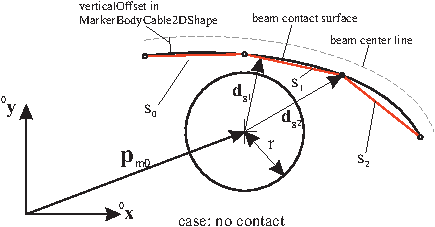
\includegraphics[width=12cm]{figures/ContactFrictionCircleCable2D.pdf}
      \end{center}
      \caption{Sketch of cable, contact segments and circle; showing case without contact, $|\dv_{g1}| > r$, 
               while contact occurs with $|\dv_{g1}| \le r$; the shortest distance vector $\dv_{g1}$
               is related to segment $s_1$ (which is perpendicular to the the segment line) and 
               $\dv_{g2}$ is the shortest distance to the end point of segment $s_2$, not being
               perpendicular.}
        \label{fig:ObjectContactFrictionCircleCable2D:sketch}
    \end{figure}
    }
    \onlyRST{
    .. _fig-objectcontactfrictioncirclecable2d-sketch:
    .. figure:: docs/theDoc/figures/ContactFrictionCircleCable2D.png
       :width: 600

       Sketch of cable, contact segments and circle; showing case without contact, $|\mathbf{d}_{g1}| > r$, while contact occurs with $|\mathbf{d}_{g1}| \le r$; the shortest distance vector $\mathbf{d}_{g1}$ is related to segment $s_1$ (which is perpendicular to the the segment line) and $\mathbf{d}_{g2}$ is the shortest distance to the end point of segment $s_2$, not being perpendicular
    }
    %+++++++++++++++++++++++++++++++++++++++++++++++
    \mysubsubsubsection{Connector forces: contact geometry}
    %
    The connector represents a force element between a 'circle' (or cylinder) represented by a marker $m0$, which has position and orientation,
    and an \texttt{ANCFCable2D} beam element (denoted as 'cable') represented by a \texttt{MarkerBodyCable2DShape} $m1$.
    The cable with reference length $L$ is discretized by splitting into $n_{cs}$ straight segments $s_i$, located between points $p_i$ and $p_{i+1}$.
    Note that these points can be placed with an offset from the cable centerline, see \texttt{verticalOffset} defined in \texttt{MarkerBodyCable2DShape}.
    In order to compute the gap function for a line segment, the shortest distance of one line segment with
    points $\pv_i$, $\pv_{i+1}$ to the circle's centerpoint given by the marker $\pv_{m0}$ is computed. 
    All computations here are performed in the global coordinates system (0), 
    including edge points of every segment.

    With the intermediate quantities (all of them related to segment $s_i$)\footnote{we omit $s_i$ in some terms for brevity!},
    \be
      \vv_s = \pv_{i+1} - \pv_i, \quad
      \vv_p = \pv_{m0} - \pv_i, \quad
      n = \vv_s\tp \vv_p, \quad
      d = \vv_s\tp \vv_s
    \ee
    and assuming that $d \neq 0$ (otherwise the two segment points would be identical and
    the shortest distance would be $d_g = |\vv_p|$),
    we find the relative position $\rho$ of the shortest (projected) point on the 
    segment, which runs from 0 to 1 if lying on the segment, as
    \be
      \rho = \frac{n}{d}
    \ee
    We distinguish 3 cases (see also \fig{fig:ObjectContactFrictionCircleCable2D:sketch} for cases 1 and 2):
        \bn
        \item If $\rho \le 0$, the shortest distance would be the distance to point $\pv_p=\pv_i$,
        reading 
        \be
          d_g = |\pv_{m0} - \pv_i| \quad (\rho \le 0)
        \ee
        \item If $\rho \ge 1$, the shortest distance would be the distance to point $\pv_p=\pv_{i+1}$,
        reading 
        \be
          d_g = |\pv_{m0} - \pv_{i+1}| \quad (\rho \ge 1)
        \ee
        \item Finally, if $0 < \rho < 1$, then the shortest distance has a projected point somewhere
        on the segment with the point (projected on the segment)
        \be
          \pv_p = \pv_i + \rho \cdot \vv_s
        \ee
        and the distance
        \be
          d_g = |\dv_g| = \sqrt{\vv_p\tp \vv_p - (n^2)/d}
        \ee
    \en
    Here, the shortest distance vector for every segment results from the projected point $\pv_p$ 
    of the above mentioned cases, see also \fig{fig:ObjectContactFrictionCircleCable2D:sketch},
    with the relation
    \be
      \dv_g = \dv_{g,s_i}= \pv_{m0} - \pv_p \eqDot
    \ee
    The contact gap for a specific point for segment $s_i$ is in general defined as
    \be \label{ObjectContactFrictionCircleCable2D:gap}
      g = g_{s_i} = d_g - r \eqDot
    \ee
    using $d_g = |\dv_g|$.
    
    %++++++++++++++++++++++++++++++++++++++++++++++
    \mysubsubsubsection{Contact frame and relative motion}
    %FRAME
    Irrespective of the choice of \texttt{useSegmentNormals}, the contact normal vector $\nv_{s_i}$ and tangential vector $\tv_{s_i}$ are defined per segment as
    \be
      \nv_{s_i} = \nv = [n_0, n_1]\tp = \frac{1}{|\dv_{g,s_i}|} \dv_{g,s_i}, \quad \tv_{s_i} = \tv = [-n_1, n_0]\tp
    \ee
    The vectors $\tv_{s_i}$ and $\nv_{s_i}$ define the local (contact) frame for further computations.
    
    The velocity at the closest point of the segment $s_i$ is interpolated using $\rho$ and computed as
    \be
      \dot \pv_p = (1-\rho) \cdot \vv_i + \rho \cdot \vv_{i+1}
    \ee
    Alternatively, $\dot \pv_p$ could be computed from the cable element by evaluating the velocity at the contact points, but we feel that
    this choice is more consistent with the computations at position level.
    
    The gap velocity $v_n$ ($\neq \dot g$) thus reads
    \be
      v_n = \left( \dot \pv_p - \dot \pv_{m0} \right) \nv
    \ee
    In a similar, the tangential velocity reads
    \be \label{ObjectContactFrictionCircleCable2D:vTangent}
      v_t = \left( \dot \pv_p - \dot \pv_{m0} \right) \tv
    \ee
    In case of \texttt{frictionStiffness != 0}, we continuously track the sticking position at which the cable element (or segment) and the circle 
    previously sticked together, similar as proposed by Lugr{\'i}s et al.~\cite{LugrisEscalonaDC2011}. 
    The difference here to the latter reference, is that we explicitly exclude switching from Newton's method and that Lugr{\'i}s et al.~used
    contact points, while we use linear segments.
    For a simple 1D example using this position based approach for friction, see \texttt{Examples/lugreFrictionText.py}, 
    which compares the traditional LuGre friction model \cite{CanudasDeWitEtAl1993} with the position based model with tangential stiffness. 
    %++++++++++++++++++++++++
    \ignoreRST{
    \begin{figure}[tbph]
      \begin{center}
      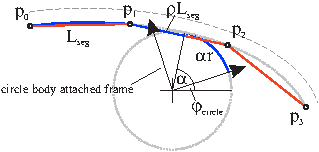
\includegraphics[width=8cm]{figures/ContactFrictionCircleCable2DstickingPos.pdf}
      \end{center}
      \caption{Calculation of last sticking position; blue parts mark the sticking position calculated as $x^*_{curStick}$.}
        \label{fig:ObjectContactFrictionCircleCable2D:stickingPos}
    \end{figure}
    }
    \onlyRST{
    .. _fig-objectcontactfrictioncirclecable2d-stickingpos:
    .. figure:: docs/theDoc/figures/ContactFrictionCircleCable2DstickingPos.png
       :width: 600

       Calculation of last sticking position; blue parts mark the sticking position calculated as $x^*_{curStick}$.
    }
    %++++++++++++++++++++++++
    
    Because there is the chance to wind/unwind relative to the (last) sticking position without slipping,
    the following strategy is used.
    In case of sliding (which could be the last time sliding before sticking), 
    we compute the {\bf current sticking position}, see \fig{fig:ObjectContactFrictionCircleCable2D:stickingPos}, as the sum of the relative position at the segment $s$
    \be
      x_{s,curStick} = \rho \cdot L_{seg}
    \ee
    in which $\rho \in [0,1]$ denotes the relative position of contact at the segment with reference length $L_{seg}=\frac{L}{n_{cs}}$.
    The relative position at the circle $c$ is
    \be
      x_{c,curStick} = \alpha \cdot r
    \ee
    We immediately see, that under pure rolling\footnote{neglecting the effects of small penetration, usually much smaller than shown for visibility in \fig{fig:ObjectContactFrictionCircleCable2D:stickingPos}.},
    \be
      x_{s,curStick} + x_{c,curStick}  = \mathrm{const}.
    \ee
    Note that the \texttt{verticalOffset} from the cable center line, as defined in the related \texttt{MarkerBodyCable2DShape},
    influences the behavior significantly, which is why we recommend to use \texttt{verticalOffset=0} whenever this is an 
    appropriate assumption.
    %include in paper:
    %Even thought that we are convinced that this has some effect, especially for beams with larger height, a reduction of segment length reduces
    %this effects as less (un-)winding occurs, a more consistent computation of this effect would require an
    %integration of relative motion as stretch influences the local changes of the relative sticking position.
    Thus, the current sticking position $x_{curStick}$ is computed per segment as
    \be  \label{ObjectContactFrictionCircleCable2D:lastCurStick}
      x^*_{curStick} = x_{s,curStick} + x_{c,curStick}, \quad
    \ee
    %
    Due to the possibility of switching of $\alpha+\phi$ between $-\pi$ and $\pi$, the result is normalized to
    \be \label{ObjectContactFrictionCircleCable2D:curStick}
      x_{curStick} = x^*_{curStick} - \mathrm{floor}\left(\frac{x^*_{curStick} }{2 \pi \cdot r} + \frac{1}{2}\right) \cdot 2 \pi \cdot r, \quad
    \ee
    which gives $\bar x_{curStick} \in [-\pi \cdot r,\pi \cdot r]$, which is stored in the 3rd data variable (per segment).
    The function floor() is a standardized version of rounding, available in C and Python programming languages.
    In the \texttt{PostNewtonStep}, the last sticking position is computed, $x_{lastStick} = x_{curStick}$, and it is also available in the \texttt{startOfStep} state.

    %++++++++++++++++++++++++++++++++++++++++++++++
    \mysubsubsubsection{Contact forces: definition}
    %FORCES
    The contact force $f_n$ is zero for $g > 0$ and otherwise computed from 
    \be \label{ObjectContactFrictionCircleCable2D:contactForce}
      f_n = k_c \cdot g + d_c \cdot v_n
    \ee
    NOTE that currently, there is only a linear spring-damper model available, assuming that the impact dynamics 
    is not dominating (such as in belt drives or reeving systems).

    Friction forces are primarily based on relative (tangential) velocity at each segment.
    The 'linear' friction force, based on the velocity penalty parameter $\mu_v$ reads
    \be
      f_t^{(lin)} = \mu_v \cdot v_t \eqComma
    \ee    
    %++++++++++++++++++++++++++++++++++++++++++++++
    \mysubsubsubsection{PostNewtonStep}
    In general, see the solver flow chart for the \texttt{DiscontinuousIteration}, see \fig{fig_solver_discontinuous_iteration}, should be considered when reading this description. Every step is started with values \texttt{startOfStep}, while current values are iterated and updated in the Newton or \texttt{DiscontinuousIteration}.
    
    The \texttt{PostNewtonStep} computes 3 values per segment, which are used for computation of contact forces, irrespectively of the 
    current geometryof the contact. 
    The \texttt{PostNewtonStep} is called after every full Newton method and evaluates the current state w.r.t. the assumed data variables.
    If the assumptions do not fit, new data variables are computed.
    This is necessary in order to avoid discontinuities in the equations, while otherwise the Newton iterations would not 
    (or only slowly) converge.

    The data variables per segment are
    \be
      [x_{gap},\, x_{isSlipStick},\, x_{lastStick}]
    \ee
    Here, $x_{gap}$ contains the gap of the segment ($\le 0$ means contact), $x_{lastStick}$ is described in 
    \eq{ObjectContactFrictionCircleCable2D:curStick}, and 
    $x_{isSlipStick}$ defines the stick or slip case,
    \bi
      \item $x_{isSlipStick} = -2$: undefined, used for initialization
      \item $x_{isSlipStick} = 0$: sticking
      \item $x_{isSlipStick} = \pm 1$: slipping, sign defines slipping direction
    \ei
    
    The basic algorithm in the \texttt{PostNewtonStep}, with all operations given for any segment $s_i$, can be summarized as follows:
    \bi
      \item[I.] Evaluate gap per segment $g$ using \eq{ObjectContactFrictionCircleCable2D:gap} and store in data variable: 
            $x_{gap} = g$
      \item[II.] If $x_{gap} < 0$ and ($\mu_v \neq 0$ or  $\mu_k \neq 0$):
      \bn
        \item Compute contact force $f_n$ according to \eq{ObjectContactFrictionCircleCable2D:contactForce}
        \item Compute current sticking position $x_{curStick}$ according to \eq{ObjectContactFrictionCircleCable2D:lastCurStick}\footnote{terms are only evaluated if $\mu_k \neq 0$}
        \item Retrieve \texttt{startOfStep} sticking position\footnote{Importantly, the \texttt{PostNewtonStep} always refers to the \texttt{startOfStep} state in the sticking position, because in the discontinuous iterations, the algorithm could switch to slipping in between and override the last sticking position in the current step} in $x^{startOfStep}_{lastStick}$ and compute and normalize
        difference in sticking position\footnote{in case that $x_{isSlipStick} = -2$, meaning that there is no stored sticking position, we set $\Delta x_{stick} = 0$}:
        \be
          \Delta x^*_{stick} = x_{curStick} - x^{startOfStep}_{lastStick}, \quad
          \Delta x_{stick} = \Delta x^*_{stick} - \mathrm{floor}\left(\frac{\Delta x^*_{stick} }{2 \pi \cdot r} + \frac{1}{2}\right) \cdot 2 \pi \cdot r
        \ee
        \item Compute linear tangential force for friction stiffness and velocity penalty: 
          \be 
            f_{t,lin} = \mu_v \cdot v_t + \mu_k \Delta x_{stick}
          \ee
        \item Compute tangential force according to Coulomb friction model \footnote{note that the sign of $\Delta x_{stick}$ is used here, but
        alternatively we may also use the sign of $f_{t,lin}$}:
        \be
            f_t = 
                \begin{cases} f_t^{(lin)}, \quad \quad \quad \quad \quad \quad \quad \mathrm{if} \quad 
                  |f_t^{(lin)}| \le \mu \cdot |f_n| \\ 
                  \mu \cdot |f_n| \cdot \mathrm{Sign}(\Delta x_{stick}), \quad \mathrm{else}
                \end{cases}          
        \ee
        \item In the case of slipping, given by $|f_t^{(lin)}| > \mu \cdot |f_n|$, we update the last sticking position in the data variable, 
        such that the spring is pre-tensioned already,
        \be
          x_{lastStick} = x_{curStick} - \mathrm{Sign}(\Delta x_{stick}) \frac{\mu \cdot |f_n|}{\mu_k}, \quad 
          x_{isSlipStick} = \mathrm{Sign}(\Delta x_{stick})
        \ee
        \item In the case of sticking, given by $|f_t^{(lin)}| \le \mu \cdot |f_n|$: Set $x_{isSlipStick} = 0$ and, 
        if $x^{startOfStep}_{isSlipStick} = -2$ (undefined), we update $x_{lastStick} = x_{curStick}$, while otherwise, $x_{lastStick}$ is unchanged.
      \en
      \item[III. ] If $x_{gap} > 0$ or ($\mu_v == 0$ and $\mu_k == 0$), we set $x_{isSlipStick} = -2$ (undefined); this means that in the next step (if this step is accepted), there is no stored sticking position.
      \item[IV.] Compute an error $\varepsilon_{PNS} = \varepsilon^n_{PNS}+\varepsilon^t_{PNS}$,
                  with physical units forces (per segment point), for \texttt{PostNewtonStep}:
      \bn
        \item if gap $x_{gap,lastPNS}$ of previous \texttt{PostNewtonStep} had different sign to current gap, set
        \be
          \varepsilon^n_{PNS} = k_c \cdot \Vert x_{gap} - x_{gap,lastPNS}\Vert
        \ee
    while otherwise $\varepsilon^n_{PNS}=0$.
        \item if stick-slip-state $x_{isSlipStick,lastPNS}$ of previous \texttt{PostNewtonStep} is different from current $x_{isSlipStick}$, set
        \be
          \varepsilon^t_{PNS} = \Vert \left(\Vert f_t^{(lin)} \Vert  - \mu \cdot |f_n| \right)\Vert 
        \ee
    while otherwise $\varepsilon^t_{PNS}=0$.
      \en
    \ei
    Note that the \texttt{PostNewtonStep} is iterated and the data variables are updated continuously until convergence, or until a max.\ number of iterations is reached. If \texttt{ignoreMaxIterations} == 0, computation will continue even if no convergence is reached after the given number of iterations. This will lead so larger errors in such steps, but may have less influence on the overall solution if such cases are rare. 

    %++++++++++++++++++++++++++++++++++++++++++++++
    \mysubsubsubsection{Computation of connector forces in Newton}
    The computation of LHS terms, the action of forces produced by the contact-friction element, is done during Newton iterations and may not have
    discontinuous behavior, thus relating computations to data variables computed in the \texttt{PostNewtonStep}.
    For efficiency, the LHS computation is only performed, if the \texttt{PostNewtonStep} determined contact in any segment.

    The operations are similar to the \texttt{PostNewtonStep}, but without switching. The following operations are performed for each segment $s_i$, if 
    $x_{gap, s_i} <= 0$:
    \bi
      \item[I.] Compute contact force $f_n$, \eq{ObjectContactFrictionCircleCable2D:contactForce}.
      \item[II.] In case of sticking ($|x_{isSlipStick}|\neq 1$):
      \bi
        \item[II.1] the current sticking position $x_{curStick}$ is computed from \eq{ObjectContactFrictionCircleCable2D:lastCurStick}, and the difference of current and last sticking position reads\footnote{see the difference to the \texttt{PostNewtonStep}: we use $x_{lastStick}$ here, not the \texttt{startOfStep} variant.}:
        \be
          \Delta x^*_{stick} = x_{curStick} - x_{lastStick}, \quad
          \Delta x_{stick} = x^*_{stick} - \mathrm{floor}\left(\frac{\Delta x^*_{stick} }{2 \pi \cdot r} + \frac{1}{2}\right) \cdot 2 \pi \cdot r
        \ee
        \item[II.2] if the friction stiffness is $\mu_k==0$ or if $x_{isSlipStick} == -2$, we set $\Delta x_{stick}=0$
        \item[II.3] using the tangential velocity from \eq{ObjectContactFrictionCircleCable2D:vTangent}, the tangent force follows as (even if it is larger than the sticking limit)
        \be
          f_t = \mu_v \cdot v_t + \mu_k \Delta x_{stick}
        \ee
    \ei
      \item[III.] In case of slipping ($|x_{isSlipStick}|=1$), the tangential firction force is set  as\footnote{see again difference to \texttt{PostNewtonStep}!},
      \be
      f_t = \mu \cdot |f_n| \cdot x_{isSlipStick}, \quad \mathrm{else}
      \ee 
    \ei
    Note that in the Newton method, the tangential force may be inconsistent with the Kuhn-Tucker conditions. However,
    the \texttt{PostNewtonStep} resolves this inconsistency.
    %++++++++++++++++++++++++++++++++++++++++++++++
    \mysubsubsubsection{Computation of LHS terms for circle and ANCF cable element}
    If \texttt{activeConnector = True}, 
    contact forces $\fv_i$ with $i \in [0,n_{cs}]$ -- these are $(n_{cs}+1)$ forces -- are applied at the points $p_i$, and they are computed for every contact segments (i.e., two segments may contribute to contact forces of one point).
    For every contact computation, first all contact forces at segment points are set to zero. 
    We distinguish two cases SN and PWN. If \texttt{useSegmentNormals==True}, we use the SN case, while otherwise the PWN case is used, 
    compare \fig{fig:ObjectContactFrictionCircleCable2D:normals}.
    %++++++++++++++++++++++++
    \ignoreRST{
    \begin{figure}[tbph]
      \begin{center}
      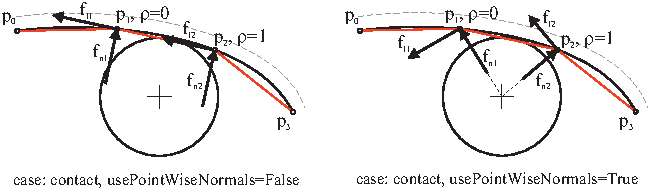
\includegraphics[width=16cm]{figures/ContactFrictionCircleCable2Dnormals.pdf}
      \end{center}
      \caption{Choice of normals and tangent vectors for calculation of normal contact forces and tangential (friction) forces; 
      note that the \texttt{useSegmentNormals=False} is not appropriate for this setup and would produce highly erroneous forces.}
        \label{fig:ObjectContactFrictionCircleCable2D:normals}
    \end{figure}
    }
    \onlyRST{
    .. _fig-objectcontactfrictioncirclecable2d-normals:
    .. figure:: docs/theDoc/figures/ContactFrictionCircleCable2Dnormals.png
       :width: 700

       Choice of normals and tangent vectors for calculation of normal contact forces and tangential (friction) forces; note that the \texttt{useSegmentNormals=False} is not appropriate for this setup and would produce highly erroneous forces.
    }
    %++++++++++++++++++++++++
    
    Segment normals (=SN) lead to always good approximations for normal directions, irrespectively of short or extremely long segments as compared to the circle. However, in case of segments that are short as compared to the circle radius, normals computed from the center of the circle to the segment points (=PWN) are more consistent and produce tangents only in circumferential direction, which may improve behavior in some applications. The equations for the two cases read:
    \bi
    \item[] \mybold{CASE SN}: use \mybold{S}egment \mybold{N}ormals\\
    If there is contact in a segment $s_i$, i.e., gap state $x_{gap} \le 0$, see \fig{fig:ObjectContactFrictionCircleCable2D:sketch}(right), contact forces $\fv_{s_i}$ are computed per segment,
    \be
      \fv_{s_i} = f_n \cdot \nv_{s_i} + f_t \tv_{s_i}
    \ee
    and added to every force at segment points according to
      \bea
        \fv_i &\pluseq& (1-\rho) \cdot \fv_{s_i}      \\ \nonumber
        \fv_{i+1} &\pluseq& \rho \cdot \fv_{s_i}
      \eea
    while in case $x_{gap}  > 0$ nothing is added.
    %     
    \item[] \mybold{CASE PWN}: use \mybold{P}oint \mybold{W}ise \mybold{N}ormals (at segment points)\\
    If there is contact in a segment $s_i$, i.e., gap $x_{gap} \le 0$, 
    see \fig{fig:ObjectContactFrictionCircleCable2D:sketch}(right), 
    intermediate contact forces $\fv^{l,r}_{i}$ are computed per segment point,
      \be
        \fv^l = f_n \cdot \nv_{l,s_i} + f_t \tv_{l,s_i}, \quad
        \fv^r = f_n \cdot \nv_{r,s_i} + f_t \tv_{r,s_i}
      \ee
      in which $\nv_{l,s_i}$ is the vector from circle center to the left point ($i$) of the segment $s_i$,
      and $\nv_{l,s_i}$ to the right point ($i+1$). The tangent vectors are perpendicular to the normals.
    %
      The forces are then applied to the contact forces $\fv_i$ using the parameter $\rho$, which takes into account the distance of contact to the left or right side of the segment,
      \bea
        \fv_i &\pluseq& (1-\rho) \cdot \fv^l      \\ \nonumber
        \fv_{i+1} &\pluseq& \rho \cdot \fv^r
      \eea
    while in case $x_{gap}  > 0$ nothing is added.
    \ei
    The forces $\fv_i$ are then applied through the marker to the \texttt{ObjectANCFCable2D} element as point loads via a position jacobian
    (using the according access function), for details see the C++ implementation.
    
    The forces on the circle marker $m0$ are computed as the total sum of all
    segment contact forces, 
    \be
      \fv_{m0} = -\sum_{s_i} \fv_{s_i} 
    \ee
    and additional torques on the circle's rotation simply follow from
    \be
      \tau_{m0} = -\sum_{s_i} r \cdot f_{t_{s_i}} \eqDot
    \ee
    %    
    During Newton iterations, the contact forces for segment $s_i$ are considered only, if 
    $x_i <= 0$. The dataCoordinate $x_i$ is not modified during Newton iterations, but computed
    during the DiscontinuousIteration, see \fig{fig_solver_discontinuous_iteration} in the solver description. 
    %
    \vspace{12pt}\\
    If \texttt{activeConnector = False}, all contact and friction forces on the cable and the force and torque on the 
    circle's marker are set to zero.
    %%RSTCOMPATIBLE
\vspace{6pt}\par\noindent\rule{\textwidth}{0.4pt}
%
\noindent For examples on ObjectContactFrictionCircleCable2D see Relevant Examples and TestModels with weblink:
\bi
\item \exuUrl{https://github.com/jgerstmayr/EXUDYN/blob/master/main/pythonDev/Examples/beltDriveALE.py}{\texttt{beltDriveALE.py}} (Examples/)
\item \exuUrl{https://github.com/jgerstmayr/EXUDYN/blob/master/main/pythonDev/Examples/beltDriveReevingSystem.py}{\texttt{beltDriveReevingSystem.py}} (Examples/)
\item \exuUrl{https://github.com/jgerstmayr/EXUDYN/blob/master/main/pythonDev/Examples/beltDrivesComparison.py}{\texttt{beltDrivesComparison.py}} (Examples/)
\item \exuUrl{https://github.com/jgerstmayr/EXUDYN/blob/master/main/pythonDev/Examples/sliderCrank3DwithANCFbeltDrive.py}{\texttt{sliderCrank3DwithANCFbeltDrive.py}} (Examples/)
\item \exuUrl{https://github.com/jgerstmayr/EXUDYN/blob/master/main/pythonDev/Examples/sliderCrank3DwithANCFbeltDrive2.py}{\texttt{sliderCrank3DwithANCFbeltDrive2.py}} (Examples/)
\item \exuUrl{https://github.com/jgerstmayr/EXUDYN/blob/master/main/pythonDev/TestModels/ANCFcontactFrictionTest.py}{\texttt{ANCFcontactFrictionTest.py}} (TestModels/)
\item \exuUrl{https://github.com/jgerstmayr/EXUDYN/blob/master/main/pythonDev/TestModels/ANCFmovingRigidBodyTest.py}{\texttt{ANCFmovingRigidBodyTest.py}} (TestModels/)
\item \exuUrl{https://github.com/jgerstmayr/EXUDYN/blob/master/main/pythonDev/TestModels/ANCFslidingAndALEjointTest.py}{\texttt{ANCFslidingAndALEjointTest.py}} (TestModels/)

\ei

%
\newpage

%+++++++++++++++++++++++++++++++++++

\mysubsubsection{ObjectContactSphereSphere}
\label{sec:item:ObjectContactSphereSphere}
[UNDER CONSTRUCTION] A simple contact connector between two spheres. The connector implements at least the same functionality as in GeneralContact and is intended for simple setups and for testing, while GeneralContact is much more efficient due to parallelization approaches and efficient contact search.
\vspace{12pt}\\

\noindent Authors: Gerstmayr Johannes, Weyrer Sebastian
\vspace{12pt}\\

\noindent \mybold{Additional information for ObjectContactSphereSphere}:
\bi
  \item This \texttt{Object} has/provides the following types = \texttt{Connector}
  \item Requested \texttt{Marker} type = \texttt{Position} + \texttt{Orientation}
  \item Requested \texttt{Node} type = \texttt{GenericData}
\ei\vspace{12pt} \noindent 
The item \mybold{ObjectContactSphereSphere} with type = 'ContactSphereSphere' has the following parameters:
\vspace{-0.5cm}\\
\vspace{-0.5cm}\\
%reference manual TABLE
\begin{center}
  \footnotesize
  \begin{longtable}{| p{4.5cm} | p{2.5cm} | p{0.5cm} | p{2.5cm} | p{6cm} |}
    \hline
    \bf Name & \bf type & \bf size & \bf default value & \bf description \\ \hline
    name &     String &      &     '' &     constraints's unique name\\ \hline
    markerNumbers &     ArrayMarkerIndex &     \tabnewline 2 &     [ invalid [-1], invalid [-1] ] &     \tabnewline list of markers representing centers of spheres, used in connector\\ \hline
    nodeNumber &     NodeIndex &      &     invalid (-1) &     \tabnewline node number of a NodeGenericData with numberOfDataCoordinates = 4 dataCoordinates, needed for discontinuous iteration (friction and contact); data variables contain values from last PostNewton iteration: data[0] is the  gap, data[1] is the norm of the tangential velocity (and thus contains information if it is stick or slip); data[2] is the impact velocity; data[3] is the plastic overlap of the Edinburgh Adhesive Elasto-Plastic Model, initialized usually with 0 and set back to 0 in case that spheres have been separated.\\ \hline
    spheresRadii &     Vector2D &     2 &     [-1.,-1.] &     \tabnewline Vector containing radius of sphere 0 and radius of sphere 1 [SI:m]\\ \hline
    dynamicFriction &     UReal &      &     0. &     dynamic friction coefficient for friction model, see StribeckFunction in exudyn.physics, \refSection{sec:module:physics}\\ \hline
    frictionProportionalZone &     UReal &      &     1e-3 &     limit velocity [m/s] up to which the friction is proportional to velocity (for regularization / avoid numerical oscillations), see StribeckFunction in exudyn.physics (named regVel there!), \refSection{sec:module:physics}\\ \hline
    contactStiffness &     UReal &      &     0. &     normal contact stiffness [SI:N/m] (units in case that $n_\mathrm{exp}=1$)\\ \hline
    contactDamping &     UReal &      &     0. &     linear normal contact damping [SI:N/(m s)]; this damping should be used (!=0) if the restitution coefficient is < 1, as it changes its behavior.\\ \hline
    contactStiffnessExponent &     PReal &      &     1. &     exponent in normal contact model [SI:1]\\ \hline
    constantPullOffForce &     UReal &      &     0. &     constant adhesion force [SI:N]; Edinburgh Adhesive Elasto-Plastic Model\\ \hline
    contactPlasticityRatio &     UReal &      &     0. &     ratio of contact stiffness for first loading and unloading/reloading [SI:1]; Edinburgh Adhesive Elasto-Plastic Model; $\lambda_\mathrm{P}=1-k_c/K2$, which gives the contact stiffness for unloading/reloading $K2 = k_c/(1-\lambda_\mathrm{P})$; set to 0 in order to fully deactivate Edinburgh Adhesive Elasto-Plastic Model model\\ \hline
    adhesionCoefficient &     UReal &      &     0. &     coefficient for adhesion [SI:N/m] (units in case that $n_\mathrm{adh}=1$); Edinburgh Adhesive Elasto-Plastic Model; set to 0 to deactivate adhesion model\\ \hline
    adhesionExponent &     UReal &      &     1. &     exponent for adhesion coefficient [SI:1]; Edinburgh Adhesive Elasto-Plastic Model\\ \hline
    restitutionCoefficient &     PReal &      &     1. &     coefficient of restitution [SI:1]; used in particular for impact mechanics; different models available within parameter impactModel; the coefficient must be > 0, but can become arbitrarily small to emulate plastic impact (however very small values may lead to numerical problems)\\ \hline
    minimumImpactVelocity &     UReal &      &     0. &     minimal impact velocity for coefficient of restitution [SI:1]; this value adds a lower bound for impact velocities for calculation of viscous impact force; it can be used to apply a larger damping behavior for low impact velocities (or permanent contact)\\ \hline
    impactModel &     UInt &      &     0 &      number of impact model: 0) linear model (only linear damping is used); 1) Hunt-Crossley model; 2) Gonthier/EtAl-Carvalho/Martins mixed model; model 2 is much more accurate regarding the coefficient of restitution, in the full range [0,1] except for 0; NOTE: in all models, the linear contactDamping still added, if not set to zero!\\ \hline
    activeConnector &     Bool &      &     True &     flag, which determines, if the connector is active; used to deactivate (temporarily) a connector or constraint\\ \hline
    visualization &     VObjectContactSphereSphere &      &      &     parameters for visualization of item\\ \hline
\end{longtable}
\end{center}

\noindent The item VObjectContactSphereSphere has the following parameters:
%reference manual TABLE
\begin{center}
  \footnotesize
  \begin{longtable}{| p{4.5cm} | p{2.5cm} | p{0.5cm} | p{2.5cm} | p{6cm} |}
    \hline
    \bf Name & \bf type & \bf size & \bf default value & \bf description \\ \hline
    show &     Bool &      &     False &     set true, if item is shown in visualization and false if it is not shown; draws spheres by given radii\\ \hline
    color &     Float4 &      &     [0.7,0.7,0.7,1.] &     \tabnewline RGBA connector color; if R==-1, use default color\\ \hline
\end{longtable}
\end{center}
\par\noindent\rule{\textwidth}{0.4pt}
\mysubsubsubsection{DESCRIPTION of ObjectContactSphereSphere:}
\label{description_ObjectContactSphereSphere}
\paragraph{Information on input parameters:} 
\startTable{input parameter}{symbol}{description see tables above}
\rowTable{markerNumbers}{$[m0,m1]\tp$}{}
\rowTable{nodeNumber}{$n_d$}{}
\rowTable{spheresRadii}{$[r_0,r_1]\tp$}{}
\rowTable{dynamicFriction}{$\mu_d$}{}
\rowTable{frictionProportionalZone}{$v_{reg}$}{}
\rowTable{contactStiffness}{$k_c$}{}
\rowTable{contactDamping}{$d_c$}{}
\rowTable{contactStiffnessExponent}{$n_\mathrm{exp}$}{}
\rowTable{constantPullOffForce}{$f_\mathrm{adh}$}{}
\rowTable{contactPlasticityRatio}{$\lambda_\mathrm{P}$}{}
\rowTable{adhesionCoefficient}{$k_\mathrm{adh}$}{}
\rowTable{adhesionExponent}{$n_\mathrm{adh}$}{}
\rowTable{restitutionCoefficient}{$e_\mathrm{res}$}{}
\rowTable{minimumImpactVelocity}{$\dot\delta_\mathrm{-,min}$}{}
\rowTable{impactModel}{$m_\mathrm{impact}$}{}
\finishTable

\mybold{The following output variables are available as OutputVariableType in sensors, Get...Output() and other functions}:
\begin{center}
\footnotesize
\begin{longtable}{| p{5cm} | p{5cm} | p{6cm} |} 
\hline
\bf output variable & \bf symbol & \bf description \\ \hline
Director3 &  & contains normalized vector from marker 0 to marker 1\\ \hline
Displacement &  & global displacement vector between the two spheres midpoints\\ \hline
DisplacementLocal &  & 3D Vector, containing only gap (Z-component)\\ \hline
Velocity &  & global relative velocity between the two spheres midpoints\\ \hline
Force &  & global contact force vector\\ \hline
Torque &  & global torque due to friction on marker 0; to obetain torque on marker 1, multiply the torque with the factor $\frac{r_1+g/2}{r_0+g/2}$\\ \hline
\end{longtable}
\end{center}
 \noindent
    \mysubsubsubsection{Definition of quantities}
    \startTable{intermediate variables}{symbol}{description}
    \rowTable{marker m0 position}{$\LU{0}{\pv}_{m0}$}{global position of sphere 0 center as provided by marker m0}
    \rowTable{marker m0 orientation}{$\LU{0,m0}{\Rot}$}{current rotation matrix provided by marker m0}
    \rowTable{marker m1 position}{$\LU{0}{\pv}_{m1}$}{global position of sphere 1 center as provided by marker m1}
    \rowTable{marker m1 orientation}{$\LU{0,m1}{\Rot}$}{current rotation matrix provided by marker m1}
    \rowTable{data coordinates}{$\xv=[x_0,\,x_1,\,x_2,\,x_3]\tp$}{hold the current gap (0), the (norm of the) tangential velocity (1), the impact velocity (2), and the plastic deformation (3) of the adhesion model}
    \rowTable{marker m0 velocity}{$\LU{0}{\vv}_{m0}$}{current global velocity which is provided by marker m0}
    \rowTable{marker m1 velocity}{$\LU{0}{\vv}_{m1}$}{current global velocity which is provided by marker m1}
    \rowTable{marker m0 angular velocity}{$\LU{0}{\tomega}_{m0}$}{current angular velocity vector provided by marker m0}
    \rowTable{marker m1 angular velocity}{$\LU{0}{\tomega}_{m1}$}{current angular velocity vector provided by marker m1}
    \finishTable
    \mysubsubsubsection{Connector Forces}
    This section outlines the computation of the forces acting on the two spheres when they are in contact with each other. Two types of forces can act on the spheres due to the connector:
    \bi
      \item normal force computed according to the chosen impact model $m_\mathrm{impact}$ and with contact damping if $d_c\neq0$; this type of force does not create a torque acting on the spheres.
      \item tangential force due to a regularized friction law to model dry friction between the spheres; this type of force creates a torque acting on the spheres and is computed independently of the chosen impact model if $\mu_d\neq0$ is set. Note that in the implemented model, rolling deformations are not considered, i.e. the friction is only a function of the relative tangential velocity between the spheres at the contact point.
    \ei

    \ignoreRST{
    \begin{figure}[tbph]
      \begin{center}
            \includegraphics[width=12cm]{figures/SphereSphereContact.pdf}
      \end{center}
        \caption{Two spheres that are in contact. For illustration, a force due to the overlap $\delta$ acting in the direction of $\nv$ for marker 1 is shown, as well as a force due to friction acting against the tangential (gap) velocity. The respective opposing forces are imprinted on marker 0.}
        \label{fig:ObjectSphereSphereContact}
    \end{figure}
    }
    \onlyRST{
    .. _fig-objectspherespherecontact-mesh:
    .. figure:: docs/theDoc/figures/SphereSphereContact.png
       :width: 400

       Two spheres that are in contact, showing a force on marker 1 in normal direction due to overlap; forces on marker 0 act in opposite direction.
    }
    For the following, the gap $g$ between the two spheres is computed as
    \be
        g = || \LU{0}{\pv}_{m1} - \LU{0}{\pv}_{m0} || - (r_0 + r_1)
    \ee
    and the overlap $\delta$ is the negated gap: $\delta=-g$. In the contact case, the overlap $\delta$ is positive. The normal vector $\LU{0}{\nv}$ points from marker 0 to marker 1 and is computed with
    \be
        \LU{0}{\nv} = \frac{\LU{0}{\pv}_{m1} - \LU{0}{\pv}_{m0}}{|| \LU{0}{\pv}_{m1} - \LU{0}{\pv}_{m0} ||} \eqDot
    \ee
    The scalar normal (gap) velocity $v_\mathrm{\delta,n}$ is computed with the velocities $\LU{0}{\vv}_{m0}=\LU{0}{\dot{\pv}}_{m0}$ and $\LU{0}{\vv}_{m1}=\LU{0}{\dot{\pv}}_{m1}$
    \be
        v_\mathrm{\delta,n} = \left(\LU{0}{\vv}_{m1} - \LU{0}{\vv}_{m0}\right)\cdot \LU{0}{\nv}
    \ee
    and the tangential (gap) velocity $\LU{0}{\vv}_\mathrm{\delta,t}$ at the contact point, that is needed for the friction model, reads
    \be \label{eq:OSSCTangentialVelocity}
        \LU{0}{\vv}_\mathrm{\delta,t} = \left(\LU{0}{\vv}_{a1} - \LU{0}{\vv}_{a0}\right) - v_\mathrm{\delta,n} \cdot \LU{0}{\nv}, \qquad v_\mathrm{rel} = || \LU{0}{\vv}_\mathrm{\delta,t} || \eqDot
    \ee
    To take the angular velocity of the spheres into account, the velocities $\LU{0}{\vv}_{a0}$ and $\LU{0}{\vv}_{a1}$ at the contact point are computed using Euler's theorem for kinematics:
    \be
        \LU{0}{\vv}_{a0} = \LU{0}{\vv}_{m0} + \LU{0}{\tomega}_{m0} \times \left(\LU{0}{\nv}\cdot \left(r_0-\frac{\delta}{2}\right)\right)
        , \qquad
        \LU{0}{\vv}_{a1} = \LU{0}{\vv}_{m1} + \LU{0}{\tomega}_{m1} \times \left(-\LU{0}{\nv}\cdot \left(r_1-\frac{\delta}{2}\right)\right) \eqDot
    \ee
    The normal force acting on marker 1 is generally written as
    \be
        \LU{0}{\fv}_\mathrm{1,n} = \underbrace{(f_c + f_d)}_{f_\mathrm{1,n}} \cdot \LU{0}{\nv} \eqComma
    \ee
    where $f_c$ is the elastic and $f_d$ the damping part. The damping $f_d$ is always computed the same, independent of the chosen impact model:
    \be
        f_d = - d_c v_\mathrm{\delta,n} \eqDot
    \ee
    The negative sign is because of the damping acting against the gap velocity: in the case of a positive normal (gap) velocity, the damping acts against $\LU{0}{\nv}$ for marker 1. The elastic force $f_c$ is computed depending on the chosen impact model.
    \bi
      \item $m_\mathrm{impact}=0$: the Adhesive Elasto-Plastic model described in \cite{Morrissey2014} is used. This model captures the key bulk behavior of cohesive powders and granular soils. For the impact model, the plastic overlap $\delta_p$ is needed. It is computed with
      \be
          \delta_p=\lambda_\mathrm{p}^{\frac{1}{n_\mathrm{exp}}}\delta \eqDot
      \ee
      The Adhesive Elasto-Plastic model distinguishes three different cases, modeling the loading and unloading behavior of the spheres:
      \be
          f_c=
          \begin{cases}
              -f_\mathrm{adh} + k_c \delta^{n_\mathrm{exp}} & \text{if } k_2 \left(\delta^{n_\mathrm{exp}}-\delta_p^{n_\mathrm{exp}} \right) \geq k_c\delta^{n_\mathrm{exp}} \\
              -f_\mathrm{adh} + k_2 \left(\delta^{n_\mathrm{exp}}-\delta_p^{n_\mathrm{exp}} \right) & \text{if } k_c\delta^{n_\mathrm{exp}} > k_2 \left(\delta^{n_\mathrm{exp}}-\delta_p^{n_\mathrm{exp}}\right) > -k_\mathrm{adh}\delta^{n_\mathrm{adh}} \\
              -f_\mathrm{adh}-k_\mathrm{adh}\delta^{n_\mathrm{adh}} & \text{if } -k_\mathrm{adh}\delta^{n_\mathrm{adh}} > k_2 \left(\delta^{n_\mathrm{exp}}-\delta_p^{n_\mathrm{exp}} \right)
          \end{cases}
          \eqDot
      \ee
    Note that $k_2$ is computed with $k_2 = k_c/(1-\lambda_\mathrm{P})$. The terms with the stiffness $k_c$ and $k_2$ have a positive sign, since they act in the direction of $\LU{0}{\nv}$ for marker 1. The constant adhesion force $f_\mathrm{adh}$ and the stiffness $k_\mathrm{adh}$ act against $\LU{0}{\nv}$, which corresponds to a force sticking the spheres together.

      \item $m_\mathrm{impact}=1$: the restitution model proposed by Hunt and Crossley in \cite{Hunt1975} is used to simulate the energy loss of the spheres during contact:
      \be
          f_c=k_c \delta^{n_\mathrm{exp}} + \lambda \delta^{n_\mathrm{exp}} v_\mathrm{\delta,n}
      \ee
      with
      \be
          \lambda = \frac{k_c}{\dot\delta_\mathrm{-}}\frac{3}{2}(e_\mathrm{res}-1) \eqDot
      \ee
      The restitution coefficient $e_\mathrm{res}$ describes the ration of the normal (gap) velocity before and after the impact of the spheres. In the case of $e_\mathrm{res}<1$, the impact has a plastic portion, resulting in a force acting against $\LU{0}{\nv}$ for marker 1, which is why $\lambda$ must be negative in that case. $\dot\delta_\mathrm{-}$ is the initial relative velocity, which is either the minimum impact velocity or the normal (negated gap) velocity:
      \be
          \dot\delta_\mathrm{-} = \max{\left(\dot\delta_\mathrm{-,min}; -v_\mathrm{\delta,n} \right)}
      \ee
    Note that the Hunt-Crossley restitution is valid for a very small energy loss ($e_\mathrm{res}\approx1$) \cite{Carvalho2019}.

      \item $m_\mathrm{impact}=2$: a generalization of the Hunt-Crossley restitution proposed by Carvalho and Martins in \cite{Carvalho2019} is used for $e_\mathrm{res} > \frac{1}{3}$ and a model proposed by Gonthier et al. in \cite{Gonthier2004} is used for impacts with a high plastic proportion, $e_\mathrm{res} < \frac{1}{3}$. Note that the two models are identical at $e_\mathrm{res} = \frac{1}{3}$. $\lambda$ is therefore computed as follows:
      \be
          \lambda=
          \begin{cases}
              \frac{k_c}{\dot\delta_\mathrm{-}}\frac{3}{2}(e_\mathrm{res}-1)\frac{11-e_\mathrm{res}}{1+9e_\mathrm{res}} & \text{if } e_\mathrm{res} > \frac{1}{3} \\
              \frac{k_c}{\dot\delta_\mathrm{-}}\frac{e_\mathrm{rep}^2-1}{e_\mathrm{rep}} & \text{if } e_\mathrm{res} > 0 \\
          \end{cases}
          \eqDot
      \ee
    \ei
    The tangential force acting on marker 1 due to the friction model acts against the tangential velocity $\vv_\mathrm{\delta,t}$, see the computation of $\vv_\mathrm{\delta,t}$ in Equation \eqref{eq:OSSCTangentialVelocity}. Thus, the tangential force for marker 1 is computed as
    \be
        \LU{0}{\fv}_\mathrm{1,t} = -\LU{0}{\vv}_\mathrm{\delta,t} \cdot
        \begin{cases}
            \frac{\mu_d f_\mathrm{1,n}}{v_{reg}} & \text{if } v_{rel} < v_{reg} \\
            \frac{\mu_d f_\mathrm{1,n}}{v_{rel}} & \text{else}\\
        \end{cases}
        \eqDot
    \ee
    Note that the case distinction above is made to ensure that for very small relative velocities the friction force does not become implausibly high. Taken together, the force acting on marker 1 due to the connector is computed as
    \be
        \LU{0}{\fv}_{m1}=\LU{0}{\fv}_\mathrm{1,n}+\LU{0}{\fv}_\mathrm{1,t} \eqComma
    \ee
    the force acting on marker 0 is $\LU{0}{\fv}_{m0}=-\LU{0}{\fv}_{m1}$. The global torque $\LU{0}{\ttau}_{m1}$ acting on marker 1 due to the connector is computed as
    \be
        \LU{0}{\ttau}_{m1}=-\LU{0}{\nv}\left( r_1-\frac{1}{2}\delta \right) \times \LU{0}{\fv}_{m1} \eqComma
    \ee
    and on marker 0 as
    \be
        \LU{0}{\ttau}_{m0}=\LU{0}{\nv} \left(r_0-\frac{1}{2}\delta \right) \times \LU{0}{\fv}_{m0}= \LU{0}{\nv}\left( r_0-\frac{1}{2}\delta \right) \times -\LU{0}{\fv}_{m1} \eqDot
    \ee
    It can be seen that the torque due to the connector is the same for both spheres, if $r_0=r_1$ applies.
    %%RSTCOMPATIBLE
\vspace{6pt}\par\noindent\rule{\textwidth}{0.4pt}
%
\noindent For examples on ObjectContactSphereSphere see Relevant Examples and TestModels with weblink:
\bi
\item \exuUrl{https://github.com/jgerstmayr/EXUDYN/blob/master/main/pythonDev/Examples/newtonsCradle.py}{\texttt{newtonsCradle.py}} (Examples/)
\item \exuUrl{https://github.com/jgerstmayr/EXUDYN/blob/master/main/pythonDev/TestModels/contactSphereSphereTest.py}{\texttt{contactSphereSphereTest.py}} (TestModels/)
\item \exuUrl{https://github.com/jgerstmayr/EXUDYN/blob/master/main/pythonDev/TestModels/contactSphereSphereTestEAPM.py}{\texttt{contactSphereSphereTestEAPM.py}} (TestModels/)

\ei

%
\newpage

%+++++++++++++++++++++++++++++++++++

\mysubsubsection{ObjectContactCurveCircles}
\label{sec:item:ObjectContactCurveCircles}
[UNDER CONSTRUCTION] A contact model between a curve defined by piecewise segments and a set of circles. The 2D curve may corotate in 3D with the underlying marker and also defines the plane of action for the circles. Note that there is a limit of 100 circle markes above which computation becomes slower as it requires memory allocation.
\vspace{12pt}\\

\noindent \mybold{Additional information for ObjectContactCurveCircles}:
\bi
  \item This \texttt{Object} has/provides the following types = \texttt{Connector}
  \item Requested \texttt{Marker} type = \texttt{Position} + \texttt{Orientation}
  \item Requested \texttt{Node} type = \texttt{GenericData}
  \item {\bf Short name} for Python = \texttt{CamFollower}
  \item {\bf Short name} for Python visualization object = \texttt{VCamFollower}
\ei\vspace{12pt} \noindent 
The item \mybold{ObjectContactCurveCircles} with type = 'ContactCurveCircles' has the following parameters:
\vspace{-0.5cm}\\
\vspace{-0.5cm}\\
%reference manual TABLE
\begin{center}
  \footnotesize
  \begin{longtable}{| p{4.5cm} | p{2.5cm} | p{0.5cm} | p{2.5cm} | p{6cm} |}
    \hline
    \bf Name & \bf type & \bf size & \bf default value & \bf description \\ \hline
    name &     String &      &     '' &     constraints's unique name\\ \hline
    markerNumbers &     ArrayMarkerIndex &     \tabnewline 2 &     [ invalid [-1], invalid [-1] ] &     \tabnewline list of $n_c+1$ markers; marker $m0$ represents the marker carrying the curve; all other markers represent centers of $n_c$ circles, used in connector\\ \hline
    nodeNumber &     NodeIndex &      &     invalid (-1) &     \tabnewline node number of a NodeGenericData with nDataVariablesPerSegment dataCoordinates per segment, needed for discontinuous iteration; data variables contain values from last PostNewton iteration: data[0+3*i] is the circle number, data[1+3*i] is the gap, data[2+3*i] is the tangential velocity (and thus contains information if it is stick or slip)\\ \hline
    circlesRadii &     NumpyVector &      &     [] &     Vector containing radii of $n_c$ circles [SI:m]; number according to size of markerNumbers-1\\ \hline
    segmentsData &     PyMatrixContainer &     \tabnewline  &     PyMatrixContainer[] &     \tabnewline matrix containing a set of two planar point coordinates in each row, representing segments attached to marker $m0$ and undergoing contact with the circles; for segment $s0$ row 0 reads $[p_{0x,s0},\,p_{0y,s0},\,p_{1x,s0},\,p_{1y,s0}]$; note that the segments must be ordered such that going from $\pv_0$ to $\pv_1$, the exterior lies on the right (positive) side. MatrixContainer has to be provided in dense mode!\\ \hline
    polynomialData &     PyMatrixContainer &     \tabnewline  &     PyMatrixContainer[] &     \tabnewline matrix containing coefficients for polynomial enhancements of the linear segments; each row contains polynomial coefficients for the according segment; the polynomial coefficients may contain quadratic, cubic, etc. coefficients, while constant and linear coefficients are automatically selected such that the end points of the polynomial match the segment's endpoints; the local coordinate $x$ of the polynomial runs from 0 to 1 and positive values represent concave geometries (enlarging the curve). MatrixContainer has to be provided in dense mode!\\ \hline
    rotationMarker0 &     Matrix3D &      &     [[1,0,0], [0,1,0], [0,0,1]] &     \tabnewline local rotation matrix for marker 0; used to rotate marker coordinates such that the curve lies in the $x-y$-plane\\ \hline
    dynamicFriction &     UReal &      &     0. &     dynamic friction coefficient for friction model, see StribeckFunction in exudyn.physics, \refSection{sec:module:physics}\\ \hline
    frictionProportionalZone &     UReal &      &     1e-3 &     limit velocity [m/s] up to which the friction is proportional to velocity (for regularization / avoid numerical oscillations), see StribeckFunction in exudyn.physics (named regVel there!), \refSection{sec:module:physics}\\ \hline
    contactStiffness &     Real &      &     0. &     normal contact stiffness [SI:N/m] (units in case that $n_\mathrm{exp}=1$)\\ \hline
    contactDamping &     Real &      &     0. &     linear normal contact damping [SI:N/(m s)]; this damping should be used (!=0) if the restitution coefficient is < 1, as it changes its behavior.\\ \hline
    contactModel &     UInt &      &     0 &     number of contact model: 0) linear model for stiffness and damping, only proportional to penetration; 1) model taking contact geometry, in particular curvature of circle and curve into account, giving nonlinear normal force model\\ \hline
    activeConnector &     Bool &      &     True &     flag, which determines, if the connector is active; used to deactivate (temporarily) a connector or constraint\\ \hline
    visualization &     VObjectContactCurveCircles &      &      &     parameters for visualization of item\\ \hline
\end{longtable}
\end{center}

\noindent The item VObjectContactCurveCircles has the following parameters:
%reference manual TABLE
\begin{center}
  \footnotesize
  \begin{longtable}{| p{4.5cm} | p{2.5cm} | p{0.5cm} | p{2.5cm} | p{6cm} |}
    \hline
    \bf Name & \bf type & \bf size & \bf default value & \bf description \\ \hline
    show &     Bool &      &     True &     set true, if item is shown in visualization and false if it is not shown; draws curve and circles with given radii; uses visualizationSettings circleTiling for circles and circleTiling/2 for tiling of non-straight segments\\ \hline
    color &     Float4 &      &     [-1.,-1.,-1.,-1.] &     \tabnewline RGBA connector color; if R==-1, use default color\\ \hline
\end{longtable}
\end{center}
\par\noindent\rule{\textwidth}{0.4pt}
\mysubsubsubsection{DESCRIPTION of ObjectContactCurveCircles:}
\label{description_ObjectContactCurveCircles}
\paragraph{Information on input parameters:} 
\startTable{input parameter}{symbol}{description see tables above}
\rowTable{markerNumbers}{$[m0,m_{c0},m_{c1},\ldots]\tp$}{}
\rowTable{nodeNumber}{$n_d$}{}
\rowTable{circlesRadii}{$[r_{c0},r_{c1}, \ldots]\tp \in \Rcal^{n_c}$}{}
\rowTable{segmentsData}{$\Dm \in \Rcal^{n_s \times 4}$}{}
\rowTable{polynomialData}{$\Pm \in \Rcal^{n_s \times n_p}$}{}
\rowTable{dynamicFriction}{$\mu_d$}{}
\rowTable{frictionProportionalZone}{$v_{reg}$}{}
\rowTable{contactStiffness}{$k_c$}{}
\rowTable{contactDamping}{$d_c$}{}
\rowTable{contactModel}{$m_\mathrm{contact}$}{}
\finishTable

\mybold{The following output variables are available as OutputVariableType in sensors, Get...Output() and other functions}:
\begin{center}
\footnotesize
\begin{longtable}{| p{5cm} | p{5cm} | p{6cm} |} 
\hline
\bf output variable & \bf symbol & \bf description \\ \hline
DisplacementLocal &  & vector containing the minimum distance to segments per circle midpoint (< 0 in case of contact, and -1 if not computed: if not in according vicinity in search tree)\\ \hline
VelocityLocal &  & vector containing relative (normal) velocity per circle midpoint (or NaN if not computed)\\ \hline
ForceLocal &  & pairs of normal and tangential forces per circle or (Nan,Nan) if not computed\\ \hline
\end{longtable}
\end{center}
 \noindent
    \mysubsubsubsection{Definition of quantities}
    \startTable{intermediate variables}{symbol}{description}
    \rowTable{marker m0 position}{$\LU{0}{\pv}_{m0}$}{global position of sphere 0 center as provided by marker m0}
    \rowTable{marker m0 orientation}{$\LU{0,m0}{\Rot}$}{current rotation matrix provided by marker m0}
    \rowTable{marker m0 velocity}{$\LU{0}{\vv}_{m0}$}{current global velocity which is provided by marker m0}
    \rowTable{marker m0 angular velocity}{$\LU{0}{\tomega}_{m0}$}{current angular velocity vector provided by marker m0}
    \rowTable{data coordinates}{$\xv=[x_0,\,x_1,\, \ldots]\tp$}{data coordinates per number of circle markers}
    \finishTable
    %
    \mysubsubsubsection{Geometric relations}
    %++++++++++++++++++++++++++++++++++++++++++++++++++++++++++
    tbd
    %%RSTCOMPATIBLE
\vspace{6pt}\par\noindent\rule{\textwidth}{0.4pt}
%
\noindent For examples on ObjectContactCurveCircles see Relevant Examples and TestModels with weblink:
\bi
\item \exuUrl{https://github.com/jgerstmayr/EXUDYN/blob/master/main/pythonDev/Examples/chainDriveExample.py}{\texttt{chainDriveExample.py}} (Examples/)

\ei

%

\newpage
%+++++++++++++++++++++++++++++++
%+++++++++++++++++++++++++++++++
\mysubsection{Objects (Constraint)}
A Constraint is a special Object and Connector, which links two or more markers. A Constraint leads to algebraic equations, which exactly fulfill special constraints on the kinematic behavior of the multibody syste, such as a constraint on a coordinate or a distance constraint.
%++++++

%+++++++++++++++++++++++++++++++++++

\mysubsubsection{ObjectConnectorDistance}
\label{sec:item:ObjectConnectorDistance}
Connector which enforces constant or prescribed distance between two bodies/nodes.
\vspace{12pt}\\

\noindent \mybold{Additional information for ObjectConnectorDistance}:
\bi
  \item This \texttt{Object} has/provides the following types = \texttt{Connector}, \texttt{Constraint}
  \item Requested \texttt{Marker} type = \texttt{Position}
  \item {\bf Short name} for Python = \texttt{DistanceConstraint}
  \item {\bf Short name} for Python visualization object = \texttt{VDistanceConstraint}
\ei\vspace{12pt} \noindent 
The item \mybold{ObjectConnectorDistance} with type = 'ConnectorDistance' has the following parameters:
\vspace{-0.5cm}\\
\vspace{-0.5cm}\\
%reference manual TABLE
\begin{center}
  \footnotesize
  \begin{longtable}{| p{4.5cm} | p{2.5cm} | p{0.5cm} | p{2.5cm} | p{6cm} |}
    \hline
    \bf Name & \bf type & \bf size & \bf default value & \bf description \\ \hline
    name &     String &      &     '' &     constraints's unique name\\ \hline
    markerNumbers &     ArrayMarkerIndex &     \tabnewline  &     [ invalid [-1], invalid [-1] ] &     \tabnewline list of markers used in connector\\ \hline
    distance &     PReal &      &     0. &     prescribed distance [SI:m] of the used markers; must by greater than zero\\ \hline
    activeConnector &     Bool &      &     True &     flag, which determines, if the connector is active; used to deactivate (temporarily) a connector or constraint\\ \hline
    visualization &     VObjectConnectorDistance &      &      &     parameters for visualization of item\\ \hline
\end{longtable}
\end{center}

\noindent The item VObjectConnectorDistance has the following parameters:
%reference manual TABLE
\begin{center}
  \footnotesize
  \begin{longtable}{| p{4.5cm} | p{2.5cm} | p{0.5cm} | p{2.5cm} | p{6cm} |}
    \hline
    \bf Name & \bf type & \bf size & \bf default value & \bf description \\ \hline
    show &     Bool &      &     True &     set true, if item is shown in visualization and false if it is not shown\\ \hline
    drawSize &     float &      &     -1. &     drawing size = link size; size == -1.f means that default connector size is used\\ \hline
    color &     Float4 &      &     [-1.,-1.,-1.,-1.] &     \tabnewline RGBA connector color; if R==-1, use default color\\ \hline
\end{longtable}
\end{center}
\par\noindent\rule{\textwidth}{0.4pt}
\mysubsubsubsection{DESCRIPTION of ObjectConnectorDistance:}
\label{description_ObjectConnectorDistance}
\paragraph{Information on input parameters:} 
\startTable{input parameter}{symbol}{description see tables above}
\rowTable{markerNumbers}{$[m0,m1]\tp$}{}
\rowTable{distance}{$d_0$}{}
\finishTable

\mybold{The following output variables are available as OutputVariableType in sensors, Get...Output() and other functions}:
\begin{center}
\footnotesize
\begin{longtable}{| p{5cm} | p{5cm} | p{6cm} |} 
\hline
\bf output variable & \bf symbol & \bf description \\ \hline
Displacement & $\LU{0}{\Delta\pv}$ & relative displacement in global coordinates\\ \hline
Velocity & $\LU{0}{\Delta\vv}$ & relative translational velocity in global coordinates\\ \hline
Distance & $|\LU{0}{\Delta\pv}|$ & distance between markers (should stay constant; shows constraint deviation)\\ \hline
Force & $\lambda_0$ & joint force (=scalar Lagrange multiplier)\\ \hline
\end{longtable}
\end{center}
 \noindent
    \mysubsubsubsection{Definition of quantities}
    \startTable{intermediate variables}{symbol}{description}
        \rowTable{marker m0 position}{$\LU{0}{\pv}_{m0}$}{current global position which is provided by marker m0}
        \rowTable{marker m1 position}{$\LU{0}{\pv}_{m1}$}{accordingly}
    %
        \rowTable{marker m0 velocity}{$\LU{0}{\vv}_{m0}$}{current global velocity which is provided by marker m0}
        \rowTable{marker m1 velocity}{$\LU{0}{\vv}_{m1}$}{accordingly}
        \rowTable{relative displacement}{$\LU{0}{\Delta\pv}$}{$\LU{0}{\pv}_{m1} - \LU{0}{\pv}_{m0}$}
        \rowTable{relative velocity}{$\LU{0}{\Delta\vv}$}{$\LU{0}{\vv}_{m1} - \LU{0}{\vv}_{m0}$}
    %
        \rowTable{algebraicVariable}{$\lambda_0$}{Lagrange multiplier = force in constraint}
    \finishTable

    \mysubsubsubsection{Connector forces constraint equations}
    If \texttt{activeConnector = True}, the index 3 algebraic equation reads
    \be
      \left|\LU{0}{\Delta\pv}\right| - d_0 = 0
    \ee
    Due to the fact that the force direction is given by
    \be
      \frac{1}{|\LU{0}{\Delta\pv}|}\LU{0}{\Delta\pv} \eqComma
    \ee
    the prescribed distance $d_0$ may not be zero. This would, otherwise, result in a change of the number of constraints.
    The index 2 (velocity level) algebraic equation reads
    \be
      \left(\frac{\LU{0}{\Delta\pv}}{\left|\LU{0}{\Delta\pv}\right|}\right)\tp \Delta\vv = 0
    \ee
    if \texttt{activeConnector = False}, the algebraic equation reads
    \be
      \lambda_0 = 0
    \ee
    %%RSTCOMPATIBLE
\vspace{6pt}\par\noindent\rule{\textwidth}{0.4pt}
\mysubsubsubsection{MINI EXAMPLE for ObjectConnectorDistance}
\label{miniExample_ObjectConnectorDistance}
\pythonstyle
\begin{lstlisting}[language=Python, firstnumber=1]
    #example with 1m pendulum, 50kg under gravity
    nMass = mbs.AddNode(NodePoint2D(referenceCoordinates=[1,0]))
    oMass = mbs.AddObject(MassPoint2D(physicsMass = 50, nodeNumber = nMass))
    
    mMass = mbs.AddMarker(MarkerNodePosition(nodeNumber=nMass))
    mGround = mbs.AddMarker(MarkerBodyPosition(bodyNumber=oGround, localPosition = [0,0,0]))
    oDistance = mbs.AddObject(DistanceConstraint(markerNumbers = [mGround, mMass], distance = 1))
    
    mbs.AddLoad(Force(markerNumber = mMass, loadVector = [0, -50*9.81, 0])) 

    #assemble and solve system for default parameters
    mbs.Assemble()
    
    sims=exu.SimulationSettings()
    sims.timeIntegration.generalizedAlpha.spectralRadius=0.7
    mbs.SolveDynamic(sims)

    #check result at default integration time
    exudynTestGlobals.testResult = mbs.GetNodeOutput(nMass, exu.OutputVariableType.Position)[0]
\end{lstlisting}

\vspace{6pt}\par\noindent\rule{\textwidth}{0.4pt}
%
\noindent For examples on ObjectConnectorDistance see Relevant Examples and TestModels with weblink:
\bi
\item \exuUrl{https://github.com/jgerstmayr/EXUDYN/blob/master/main/pythonDev/Examples/HydraulicActuatorStaticInitialization.py}{\texttt{HydraulicActuatorStaticInitialization.py}} (Examples/)
\item \exuUrl{https://github.com/jgerstmayr/EXUDYN/blob/master/main/pythonDev/Examples/pendulum2Dconstraint.py}{\texttt{pendulum2Dconstraint.py}} (Examples/)
\item \exuUrl{https://github.com/jgerstmayr/EXUDYN/blob/master/main/pythonDev/Examples/pendulumIftommBenchmark.py}{\texttt{pendulumIftommBenchmark.py}} (Examples/)
\item \exuUrl{https://github.com/jgerstmayr/EXUDYN/blob/master/main/pythonDev/TestModels/fourBarMechanismTest.py}{\texttt{fourBarMechanismTest.py}} (TestModels/)
\item \exuUrl{https://github.com/jgerstmayr/EXUDYN/blob/master/main/pythonDev/TestModels/coordinateVectorConstraint.py}{\texttt{coordinateVectorConstraint.py}} (TestModels/)
\item \exuUrl{https://github.com/jgerstmayr/EXUDYN/blob/master/main/pythonDev/TestModels/coordinateVectorConstraintGenericODE2.py}{\texttt{coordinateVectorConstraintGenericODE2.py}} (TestModels/)
\item \exuUrl{https://github.com/jgerstmayr/EXUDYN/blob/master/main/pythonDev/TestModels/modelUnitTests.py}{\texttt{modelUnitTests.py}} (TestModels/)
\item \exuUrl{https://github.com/jgerstmayr/EXUDYN/blob/master/main/pythonDev/TestModels/PARTS_ATEs_moving.py}{\texttt{PARTS\_ATEs\_moving.py}} (TestModels/)

\ei

%
\newpage

%+++++++++++++++++++++++++++++++++++

\mysubsubsection{ObjectConnectorCoordinate}
\label{sec:item:ObjectConnectorCoordinate}
A coordinate constraint which constrains two (scalar) coordinates of Marker[Node|Body]Coordinates attached to nodes or bodies. The constraint acts directly on coordinates, but does not include reference values, e.g., of nodal values. This constraint is computationally efficient and should be used to constrain nodal coordinates.
\vspace{12pt}\\

\noindent \mybold{Additional information for ObjectConnectorCoordinate}:
\bi
  \item This \texttt{Object} has/provides the following types = \texttt{Connector}, \texttt{Constraint}
  \item Requested \texttt{Marker} type = \texttt{Coordinate}
  \item {\bf Short name} for Python = \texttt{CoordinateConstraint}
  \item {\bf Short name} for Python visualization object = \texttt{VCoordinateConstraint}
\ei\vspace{12pt} \noindent 
The item \mybold{ObjectConnectorCoordinate} with type = 'ConnectorCoordinate' has the following parameters:
\vspace{-0.5cm}\\
\vspace{-0.5cm}\\
%reference manual TABLE
\begin{center}
  \footnotesize
  \begin{longtable}{| p{4.5cm} | p{2.5cm} | p{0.5cm} | p{2.5cm} | p{6cm} |}
    \hline
    \bf Name & \bf type & \bf size & \bf default value & \bf description \\ \hline
    name &     String &      &     '' &     constraints's unique name\\ \hline
    markerNumbers &     ArrayMarkerIndex &     \tabnewline  &     [ invalid [-1], invalid [-1] ] &     \tabnewline list of markers used in connector\\ \hline
    offset &     Real &      &     0. &     An offset between the two values\\ \hline
    factorValue1 &     Real &      &     1. &     An additional factor multiplied with value1 used in algebraic equation\\ \hline
    velocityLevel &     Bool &      &     False &     If true: connector constrains velocities (only works for \hac{ODE2} coordinates!); offset is used between velocities; in this case, the offsetUserFunction\_t is considered and offsetUserFunction is ignored\\ \hline
    offsetUserFunction &     PyFunctionMbsScalarIndexScalar &     \tabnewline  &     \tabnewline 0 &     A Python function which defines the time-dependent offset; see description below\\ \hline
    offsetUserFunction\_t &     PyFunctionMbsScalarIndexScalar &     \tabnewline  &     \tabnewline 0 &     time derivative of offsetUserFunction; needed for velocity level constraints; see description below\\ \hline
    activeConnector &     Bool &      &     True &     flag, which determines, if the connector is active; used to deactivate (temporarily) a connector or constraint\\ \hline
    visualization &     VObjectConnectorCoordinate &      &      &     parameters for visualization of item\\ \hline
\end{longtable}
\end{center}

\noindent The item VObjectConnectorCoordinate has the following parameters:
%reference manual TABLE
\begin{center}
  \footnotesize
  \begin{longtable}{| p{4.5cm} | p{2.5cm} | p{0.5cm} | p{2.5cm} | p{6cm} |}
    \hline
    \bf Name & \bf type & \bf size & \bf default value & \bf description \\ \hline
    show &     Bool &      &     True &     set true, if item is shown in visualization and false if it is not shown\\ \hline
    drawSize &     float &      &     -1. &     drawing size = link size; size == -1.f means that default connector size is used\\ \hline
    color &     Float4 &      &     [-1.,-1.,-1.,-1.] &     \tabnewline RGBA connector color; if R==-1, use default color\\ \hline
\end{longtable}
\end{center}
\par\noindent\rule{\textwidth}{0.4pt}
\mysubsubsubsection{DESCRIPTION of ObjectConnectorCoordinate:}
\label{description_ObjectConnectorCoordinate}
\paragraph{Information on input parameters:} 
\startTable{input parameter}{symbol}{description see tables above}
\rowTable{markerNumbers}{$[m0,m1]\tp$}{}
\rowTable{offset}{$l_\mathrm{off}$}{}
\rowTable{factorValue1}{$k_{m1}$}{}
\rowTable{offsetUserFunction}{$\mathrm{UF} \in \Rcal$}{}
\rowTable{offsetUserFunction\_t}{$\mathrm{UF}_t \in \Rcal$}{}
\finishTable

\mybold{The following output variables are available as OutputVariableType in sensors, Get...Output() and other functions}:
\begin{center}
\footnotesize
\begin{longtable}{| p{5cm} | p{5cm} | p{6cm} |} 
\hline
\bf output variable & \bf symbol & \bf description \\ \hline
Displacement & $\Delta q$ & relative scalar displacement of marker coordinates, not including factorValue1\\ \hline
Velocity & $\Delta v$ & difference of scalar marker velocity coordinates, not including factorValue1\\ \hline
ConstraintEquation & $\cv$ & (residuum of) constraint equation\\ \hline
Force & $\lambda_0$ & scalar constraint force (Lagrange multiplier)\\ \hline
\end{longtable}
\end{center}
 \noindent
    \mysubsubsubsection{Definition of quantities}
    \startTable{intermediate variables}{symbol}{description}
    \rowTable{marker m0 coordinate}{$q_{m0}$}{current displacement coordinate which is provided by marker m0; does NOT include reference coordinate!}
    \rowTable{marker m1 coordinate}{$q_{m1}$}{}
    \rowTable{marker m0 velocity coordinate}{$v_{m0}$}{current velocity coordinate which is provided by marker m0}
    \rowTable{marker m1 velocity coordinate}{$v_{m1}$}{}
    \rowTable{difference of coordinates}{$\Delta q = q_{m1} - q_{m0}$}{Displacement between marker m0 to marker m1 coordinates (does NOT include reference coordinates)}
    \rowTable{difference of velocity coordinates}{$\Delta v= v_{m1} - v_{m0}$}{}
    \finishTable
    \mysubsubsubsection{Connector constraint equations}
    If \texttt{activeConnector = True}, the index 3 algebraic equation reads
    \be
      \cv(q_{m0}, q_{m1}) = k_{m1} \cdot q_{m1} - q_{m0} - l_\mathrm{off} = 0
    \ee
    If the offsetUserFunction $\mathrm{UF}$ is defined, $\cv$ instead becomes ($t$ is current time)
    \be
      \cv(q_{m0}, q_{m1}) = k_{m1} \cdot q_{m1} - q_{m0} -  \mathrm{UF}(mbs, t, i_N, l_\mathrm{off}) = 0
    \ee
    The \texttt{activeConnector = True}, index 2 (velocity level) algebraic equation reads
    \be
      \dot \cv(\dot q_{m0}, \dot q_{m1}) = k_{m1} \cdot \dot q_{m1} - \dot q_{m0} - d = 0
    \ee
    The factor $d$ in velocity level equations is zero, except if parameters.velocityLevel = True, then $d=l_\mathrm{off}$.
    If velocity level constraints are active and the velocity level offsetUserFunction\_t $\mathrm{UF}_t$ is defined, $\dot \cv$ instead becomes ($t$ is current time)
    \be
      \dot \cv(\dot q_{m0}, \dot q_{m1}) = k_{m1} \cdot \dot q_{m1} - \dot q_{m0} - \mathrm{UF}_t(mbs, t, i_N, l_\mathrm{off}) = 0
    \ee
    and \texttt{iN} represents the itemNumber (=objectNumber).
    Note that the index 2 equations are used, if the solver uses index 2 formulation OR if the flag parameters.velocityLevel = True (or both).
    The user functions include dependency on time $t$, but this time dependency is not respected in the computation of initial accelerations. Therefore,
    it is recommended that $\mathrm{UF}$ and $\mathrm{UF}_t$ does not include initial accelerations.

    If \texttt{activeConnector = False}, the (index 1) algebraic equation reads for ALL cases:
    \be
      \cv(\lambda_0) = \lambda_0 = 0
    \ee
    %
    %++++++++++++++++++++++++++++++++++++++++++++++++++++++++++
    \userFunction{offsetUserFunction(mbs, t, itemNumber, lOffset)}
    %
    A user function, which computes scalar offset for the coordinate constraint, e.g., in order to move a node on a prescribed trajectory.
    It is NECESSARY to use sufficiently smooth functions, having {\bf initial offsets} consistent with {\bf initial configuration} of bodies, 
    either zero or compatible initial offset-velocity, and no initial accelerations.
    The \texttt{offsetUserFunction} is {\bf ONLY used} in case of static computation or index3 (generalizedAlpha) time integration.
    In order to be on the safe side, provide both  \texttt{offsetUserFunction} and  \texttt{offsetUserFunction\_t}.

    Note that itemNumber represents the index of the object in mbs, which can be used to retrieve additional data from the object through
    \texttt{mbs.GetObjectParameter(itemNumber, ...)}, see the according description of \texttt{GetObjectParameter}.

    The user function gets time and the offset parameter as an input and returns the computed offset:
    %
    \startTable{arguments / return}{type or size}{description}
      \rowTable{\texttt{mbs}}{MainSystem}{provides MainSystem mbs in which underlying item is defined}
      \rowTable{\texttt{t}}{Real}{current time in mbs} %use t instead time in order to avoid possible conflicts with Python time
      \rowTable{\texttt{itemNumber}}{Index}{integer number $i_N$ of the object in mbs, allowing easy access to all object data via mbs.GetObjectParameter(itemNumber, ...)}
      \rowTable{\texttt{lOffset}}{Real}{$l_\mathrm{off}$}
      \rowTable{\returnValue}{Real}{computed offset for given time}
    \finishTable
    %
    %++++++++++++++++++++++++++++++++++++++++++++++++++++++++++
    \userFunction{offsetUserFunction\_t(mbs, t, itemNumber, lOffset)}
    %
    A user function, which computes scalar offset {\bf velocity} for the coordinate constraint.
    It is NECESSARY to use sufficiently smooth functions, having {\bf initial offset velocities} consistent with {\bf initial velocities} of bodies.
    The \texttt{offsetUserFunction\_t} is used instead of \texttt{offsetUserFunction} in case of \texttt{velocityLevel = True}, 
    or for index2 time integration and needed for computation of initial accelerations in second order implicit time integrators.

    Note that itemNumber represents the index of the object in mbs, which can be used to retrieve additional data from the object through
    \texttt{mbs.GetObjectParameter(itemNumber, ...)}, see the according description of \texttt{GetObjectParameter}.

    The user function gets time and the offset parameter as an input and returns the computed offset velocity:
    %
    \startTable{arguments / return}{type or size}{description}
      \rowTable{\texttt{mbs}}{MainSystem}{provides MainSystem mbs in which underlying item is defined}
      \rowTable{\texttt{t}}{Real}{current time in mbs} %use t instead time in order to avoid possible conflicts with Python time
      \rowTable{\texttt{itemNumber}}{Index}{integer number of the object in mbs, allowing easy access to all object data via mbs.GetObjectParameter(itemNumber, ...)}
      \rowTable{\texttt{lOffset}}{Real}{$l_\mathrm{off}$}
      \rowTable{\returnValue}{Real}{computed offset velocity for given time}
    \finishTable
    %
    %++++++++++++++++++++++++++++++++++++++++++++++++++++++++++
    \userFunctionExample{}
    \pythonstyle\begin{lstlisting}
        #see also mini example!
        from math import sin, cos, pi
        def UFoffset(mbs, t, itemNumber, lOffset): 
            return 0.5*lOffset*(1-cos(0.5*pi*t))
        
        def UFoffset_t(mbs, t, itemNumber, lOffset): #time derivative of UFoffset
            return 0.5*lOffset*0.5*pi*sin(0.5*pi*t)

        nMass=mbs.AddNode(Point(referenceCoordinates = [2,0,0]))
        massPoint = mbs.AddObject(MassPoint(physicsMass = 5, nodeNumber = nMass))
        
        groundMarker=mbs.AddMarker(MarkerNodeCoordinate(nodeNumber= nGround, coordinate = 0))
        nodeMarker  =mbs.AddMarker(MarkerNodeCoordinate(nodeNumber= nMass, coordinate = 0))
        
        #Spring-Damper between two marker coordinates
        mbs.AddObject(CoordinateConstraint(markerNumbers = [groundMarker, nodeMarker], 
                                           offset = 0.1, 
                                           offsetUserFunction = UFoffset, 
                                           offsetUserFunction_t = UFoffset_t)) 
    \end{lstlisting}
    %%RSTCOMPATIBLE
\vspace{6pt}\par\noindent\rule{\textwidth}{0.4pt}
\mysubsubsubsection{MINI EXAMPLE for ObjectConnectorCoordinate}
\label{miniExample_ObjectConnectorCoordinate}
\pythonstyle
\begin{lstlisting}[language=Python, firstnumber=1]
    def OffsetUF(mbs, t, itemNumber, lOffset): #gives 0.05 at t=1
        return 0.5*(1-np.cos(2*3.141592653589793*0.25*t))*lOffset

    nMass=mbs.AddNode(Point(referenceCoordinates = [2,0,0]))
    massPoint = mbs.AddObject(MassPoint(physicsMass = 5, nodeNumber = nMass))
    
    groundMarker=mbs.AddMarker(MarkerNodeCoordinate(nodeNumber= nGround, coordinate = 0))
    nodeMarker  =mbs.AddMarker(MarkerNodeCoordinate(nodeNumber= nMass, coordinate = 0))
    
    #Spring-Damper between two marker coordinates
    mbs.AddObject(CoordinateConstraint(markerNumbers = [groundMarker, nodeMarker], 
                                       offset = 0.1, offsetUserFunction = OffsetUF)) 

    #assemble and solve system for default parameters
    mbs.Assemble()
    mbs.SolveDynamic()

    #check result at default integration time
    exudynTestGlobals.testResult  = mbs.GetNodeOutput(nMass, exu.OutputVariableType.Displacement)[0]
\end{lstlisting}

\vspace{6pt}\par\noindent\rule{\textwidth}{0.4pt}
%
\noindent For examples on ObjectConnectorCoordinate see Relevant Examples and TestModels with weblink:
\bi
\item \exuUrl{https://github.com/jgerstmayr/EXUDYN/blob/master/main/pythonDev/Examples/NGsolveModalAnalysis.py}{\texttt{NGsolveModalAnalysis.py}} (Examples/)
\item \exuUrl{https://github.com/jgerstmayr/EXUDYN/blob/master/main/pythonDev/Examples/sliderCrank3DwithANCFbeltDrive2.py}{\texttt{sliderCrank3DwithANCFbeltDrive2.py}} (Examples/)
\item \exuUrl{https://github.com/jgerstmayr/EXUDYN/blob/master/main/pythonDev/Examples/ALEANCFpipe.py}{\texttt{ALEANCFpipe.py}} (Examples/)
\item \exuUrl{https://github.com/jgerstmayr/EXUDYN/blob/master/main/pythonDev/Examples/ANCFALEtest.py}{\texttt{ANCFALEtest.py}} (Examples/)
\item \exuUrl{https://github.com/jgerstmayr/EXUDYN/blob/master/main/pythonDev/Examples/ANCFcantileverTestDyn.py}{\texttt{ANCFcantileverTestDyn.py}} (Examples/)
\item \exuUrl{https://github.com/jgerstmayr/EXUDYN/blob/master/main/pythonDev/Examples/ANCFcontactCircle.py}{\texttt{ANCFcontactCircle.py}} (Examples/)
\item \exuUrl{https://github.com/jgerstmayr/EXUDYN/blob/master/main/pythonDev/Examples/ANCFcontactCircle2.py}{\texttt{ANCFcontactCircle2.py}} (Examples/)
\item \exuUrl{https://github.com/jgerstmayr/EXUDYN/blob/master/main/pythonDev/Examples/ANCFmovingRigidbody.py}{\texttt{ANCFmovingRigidbody.py}} (Examples/)
\item \exuUrl{https://github.com/jgerstmayr/EXUDYN/blob/master/main/pythonDev/Examples/ANCFrotatingCable2D.py}{\texttt{ANCFrotatingCable2D.py}} (Examples/)
\item \exuUrl{https://github.com/jgerstmayr/EXUDYN/blob/master/main/pythonDev/Examples/ANCFslidingJoint2D.py}{\texttt{ANCFslidingJoint2D.py}} (Examples/)
\item \exuUrl{https://github.com/jgerstmayr/EXUDYN/blob/master/main/pythonDev/Examples/ANCFslidingJoint2Drigid.py}{\texttt{ANCFslidingJoint2Drigid.py}} (Examples/)
\item \exuUrl{https://github.com/jgerstmayr/EXUDYN/blob/master/main/pythonDev/Examples/ANCFswitchingSlidingJoint2D.py}{\texttt{ANCFswitchingSlidingJoint2D.py}} (Examples/)
\item  ...

\item \exuUrl{https://github.com/jgerstmayr/EXUDYN/blob/master/main/pythonDev/TestModels/ANCFBeamTest.py}{\texttt{ANCFBeamTest.py}} (TestModels/)
\item \exuUrl{https://github.com/jgerstmayr/EXUDYN/blob/master/main/pythonDev/TestModels/ANCFbeltDrive.py}{\texttt{ANCFbeltDrive.py}} (TestModels/)
\item \exuUrl{https://github.com/jgerstmayr/EXUDYN/blob/master/main/pythonDev/TestModels/ANCFcontactCircleTest.py}{\texttt{ANCFcontactCircleTest.py}} (TestModels/)
\item  ...


\ei

%
\newpage

%+++++++++++++++++++++++++++++++++++

\mysubsubsection{ObjectConnectorCoordinateVector}
\label{sec:item:ObjectConnectorCoordinateVector}
A constraint which constrains the coordinate vectors of two markers Marker[Node|Object|Body]Coordinates attached to nodes or bodies. The marker uses the objects \ac{LTG}-lists to build the according coordinate mappings.
\vspace{12pt}\\

\noindent \mybold{Additional information for ObjectConnectorCoordinateVector}:
\bi
  \item This \texttt{Object} has/provides the following types = \texttt{Connector}, \texttt{Constraint}
  \item Requested \texttt{Marker} type = \texttt{Coordinate}
  \item {\bf Short name} for Python = \texttt{CoordinateVectorConstraint}
  \item {\bf Short name} for Python visualization object = \texttt{VCoordinateVectorConstraint}
\ei\vspace{12pt} \noindent 
The item \mybold{ObjectConnectorCoordinateVector} with type = 'ConnectorCoordinateVector' has the following parameters:
\vspace{-0.5cm}\\
\vspace{-0.5cm}\\
%reference manual TABLE
\begin{center}
  \footnotesize
  \begin{longtable}{| p{4.5cm} | p{2.5cm} | p{0.5cm} | p{2.5cm} | p{6cm} |}
    \hline
    \bf Name & \bf type & \bf size & \bf default value & \bf description \\ \hline
    name &     String &      &     '' &     constraints's unique name\\ \hline
    markerNumbers &     ArrayMarkerIndex &     \tabnewline  &     [ invalid [-1], invalid [-1] ] &     \tabnewline list of markers used in connector\\ \hline
    scalingMarker0 &     NumpyMatrix &      &     Matrix[] &     linear scaling matrix for coordinate vector of marker 0; matrix provided in Python numpy format\\ \hline
    scalingMarker1 &     NumpyMatrix &      &     Matrix[] &     linear scaling matrix for coordinate vector of marker 1; matrix provided in Python numpy format\\ \hline
    quadraticTermMarker0 &     NumpyMatrix &      &     Matrix[] &     quadratic scaling matrix for coordinate vector of marker 0; matrix provided in Python numpy format\\ \hline
    quadraticTermMarker1 &     NumpyMatrix &      &     Matrix[] &     quadratic scaling matrix for coordinate vector of marker 1; matrix provided in Python numpy format\\ \hline
    offset &     NumpyVector &      &     [] &     offset added to constraint equation; only active, if no userFunction is defined\\ \hline
    velocityLevel &     Bool &      &     False &     If true: connector constrains velocities (only works for \hac{ODE2} coordinates!); offset is used between velocities; in this case, the offsetUserFunction\_t is considered and offsetUserFunction is ignored\\ \hline
    constraintUserFunction &     PyFunctionVectorMbsScalarIndex2VectorBool &     \tabnewline  &     \tabnewline 0 &     \tabnewline A Python user function which computes the constraint equations; to define the number of algebraic equations, set scalingMarker0 as a numpy.zeros((nAE,1)) array with nAE being the number algebraic equations; see description below\\ \hline
    jacobianUserFunction &     PyFunctionMatrixContainerMbsScalarIndex2VectorBool &     \tabnewline  &     \tabnewline 0 &     \tabnewline A Python user function which computes the jacobian, i.e., the derivative of the left-hand-side object equation w.r.t.\ the coordinates (times $f_{ODE2}$) and w.r.t.\ the velocities (times $f_{ODE2_t}$). Terms on the RHS must be subtracted from the LHS equation; the respective terms for the stiffness matrix and damping matrix are automatically added; see description below\\ \hline
    activeConnector &     Bool &      &     True &     flag, which determines, if the connector is active; used to deactivate (temporarily) a connector or constraint\\ \hline
    visualization &     VObjectConnectorCoordinateVector &      &      &     parameters for visualization of item\\ \hline
\end{longtable}
\end{center}

\noindent The item VObjectConnectorCoordinateVector has the following parameters:
%reference manual TABLE
\begin{center}
  \footnotesize
  \begin{longtable}{| p{4.5cm} | p{2.5cm} | p{0.5cm} | p{2.5cm} | p{6cm} |}
    \hline
    \bf Name & \bf type & \bf size & \bf default value & \bf description \\ \hline
    show &     Bool &      &     True &     set true, if item is shown in visualization and false if it is not shown\\ \hline
    color &     Float4 &      &     [-1.,-1.,-1.,-1.] &     \tabnewline RGBA connector color; if R==-1, use default color\\ \hline
\end{longtable}
\end{center}
\par\noindent\rule{\textwidth}{0.4pt}
\mysubsubsubsection{DESCRIPTION of ObjectConnectorCoordinateVector:}
\label{description_ObjectConnectorCoordinateVector}
\paragraph{Information on input parameters:} 
\startTable{input parameter}{symbol}{description see tables above}
\rowTable{markerNumbers}{$[m0,m1]\tp$}{}
\rowTable{scalingMarker0}{$\Xm_{m0} \in \Rcal^{n_{ae} \times n_{q_{m0}}}$}{}
\rowTable{scalingMarker1}{$\Xm_{m1} \in \Rcal^{n_{ae} \times n_{q_{m1}}}$}{}
\rowTable{quadraticTermMarker0}{$\Ym_{m0} \in \Rcal^{n_{ae} \times n_{q_{m0}}}$}{}
\rowTable{quadraticTermMarker1}{$\Ym_{m0} \in \Rcal^{n_{ae} \times n_{q_{m0}}}$}{}
\rowTable{offset}{$\vv_\mathrm{off} \in \Rcal^{n_{ae}}$}{}
\rowTable{constraintUserFunction}{$\cv_{user} \in \Rcal^{n_{ae}}$}{}
\rowTable{jacobianUserFunction}{$\Jm_{user} \in \Rcal^{(n_{q_{m0}}+n_{q_{m1}}) \times n_{ae}}$}{}
\finishTable

\mybold{The following output variables are available as OutputVariableType in sensors, Get...Output() and other functions}:
\begin{center}
\footnotesize
\begin{longtable}{| p{5cm} | p{5cm} | p{6cm} |} 
\hline
\bf output variable & \bf symbol & \bf description \\ \hline
Displacement & $\Delta \qv$ & relative scalar displacement of marker coordinates, not including scaling matrices\\ \hline
Velocity & $\Delta \vv$ & difference of scalar marker velocity coordinates, not including scaling matrices\\ \hline
ConstraintEquation & $\cv$ & (residuum of) constraint equations\\ \hline
Force & $\tlambda$ & constraint force vector (vector of Lagrange multipliers), resulting from action of constraint equations\\ \hline
\end{longtable}
\end{center}
 \noindent
    \mysubsubsubsection{Definition of quantities}
    \startTable{intermediate variables}{symbol}{description}
    \rowTable{marker m0 coordinate vector}{$\qv_{m0} \in \Rcal^{n_{q_{m0}}}$}{coordinate vector provided by marker $m0$; depending on the marker, the coordinates may or may not include reference coordinates}
    \rowTable{marker m1 coordinate vector}{$\qv_{m1} \in \Rcal^{n_{q_{m1}}}$}{coordinate vector provided by marker $m1$; depending on the marker, the coordinates may or may not include reference coordinates}
    \rowTable{marker m0 velocity coordinate vector}{$\dot \qv_{m0} \in \Rcal^{n_{q_{m0}}}$}{velocity coordinate vector provided by marker $m0$}
    \rowTable{marker m1 velocity coordinate vector}{$\dot \qv_{m1} \in \Rcal^{n_{q_{m1}}}$}{velocity coordinate vector provided by marker $m1$}
    \rowTable{number of algebraic equations}{$n_{ae}$}{number of algebraic equations must be same as number of rows in $\Xm_{m0}$ and $\Xm_{m1}$}
    %
    \rowTable{difference of coordinates}{$\Delta \qv = \qv_{m1} - \qv_{m0}$}{Displacement between marker m0 to marker m1 coordinates}
    \rowTable{difference of velocity coordinates}{$\Delta \vv= \dot \qv_{m1} - \dot \qv_{m0}$}{}
    \finishTable
    %
    \mysubsubsubsection{Remarks}
    The number of algebraic equations depends on the maximum number of rows in $\Xm_{m0}$, $\Ym_{m0}$, $\Xm_{m1}$ and $\Ym_{m1}$. 
    The number of rows of the latter matrices must either be zero or the maximum of these rows.

    The number of columns in $\Xm_{m0}$ (or $\Ym_{m0}$) must agree with the length of the coordinate vector
    $\qv_{m0}$ and the number of columns in $\Xm_{m1}$ (or $\Ym_{m1}$) must agree with the length of the coordinate vector
    $\qv_{m1}$, if these matrices are not empty matrices. 
    If one marker $k$ is a ground marker (node/object), the length of $\qv_{m,k}$ is zero and also the according matrices
    $\Xm_{m,k}$, $\Ym_{m,k}$  have zero size and will not be considered in the computation of the constraint equations.

    %If the number of rows of $\Xm_{m0}$ plus the number of rows of $\Xm_{m1}$ is
    %larger than the total number of coordinates ( $\qv_{m0}$ and  $\qv_{m1}$), the algebraic equations are 
    %underdetermined and probably not solvable.

    \mysubsubsubsection{Connector constraint equations}
    If \texttt{activeConnector = True} and no \texttt{constraintUserFunction} is defined, the index 3 algebraic equations
    \be
      \cv(\qv_{m0}, \qv_{m1}) = \Xm_{m1} \cdot \qv_{m1} 
      + \Ym_{m1} \cdot \qv^2_{m1} %quadratic terms have been excluded, as it could not be used for Euler Parameter constraints!
      - \Xm_{m0} \cdot\qv_{m0} 
      - \Ym_{m0} \cdot\qv^2_{m0} 
      - \vv_\mathrm{off} = 0
    \ee
    Note that the squared coordinates are understood as $\qv^2_{m0} = [q^2_{0,m0}, \; q^2_{1,m0}, \; \ldots]\tp$, same for $\qv^2_{m1}$.

    The index 2 (velocity level) algebraic equation accordingly reads
    \be
      \dot \cv(\dot \qv_{m0}, \dot \qv_{m1}) = \Xm_{m1} \cdot \dot \qv_{m1} 
      + \Ym_{m1} \cdot \dot \qv^2_{m1} 
      - \Xm_{m0} \cdot \dot \qv_{m0} 
      - \Ym_{m0} \cdot \dot \qv^2_{m0} 
      - \dv_\mathrm{off} = 0
    \ee
    The vector $\dv$ in velocity level equations is zero, except if \texttt{parameters.velocityLevel = True}, then $\dv=\vv_\mathrm{off}$.

    Note that the index 2 equations are used, if the solver uses index 2 formulation OR if the flag \texttt{parameters.velocityLevel = True} (or both).
    However, the \texttt{constraintUserFunction} has to be chosen accordingly by the user, either as position or as velocity level.
    The user functions include dependency on time $t$, but this time dependency is not respected in the computation of initial accelerations. Therefore,

    If \texttt{activeConnector = False}, the (index 1) algebraic equation reads for ALL cases:
    \be
      \cv(\tlambda) = \tlambda = 0
    \ee


    If a \texttt{constraintUserFunction} is defined, it also requires an according \texttt{jacobianUserFunction} (and vice versa).
    %without $\Km$ and $\Dm$ (these matrices are added internally),
    %\be \label{eq_ObjectGenericODE2_Jac}
    %  \Jm_{user}(mbs, t, i_N, \qv, \dot \qv, f_{ODE2}, f_{ODE2_t}) =
    %        -f_{ODE2}   \left(\frac{\partial \fv_{user}(mbs, t, i_N,\qv,\dot \qv)}{\partial \qv} \right) - 
    %         f_{ODE2_t} \left(\frac{\partial \fv_{user}(mbs, t, i_N,\qv,\dot \qv)}{\partial \dot \qv} \right)
    %\ee
    %CoordinateLoads are added for the respective \hac{ODE2} coordinate on the RHS of the latter equation.
    %
    %++++++++++++++++++++++++++++++++++++++++++++++++++++++++++
    \userFunction{constraintUserFunction(mbs, t, itemNumber, q, q\_t, velocityLevel)}
    A user function, which computes algebraic equations for the connector based on the marker coordinates stored in \texttt{q} and \texttt{q\_t}.
    Depending on \texttt{velocityLevel}, the user function needs to compute either the position-level (\texttt{velocityLevel=False}) or
    the velocity level (\texttt{velocityLevel=True}) constraint equations.
    Note that for Index 2 solvers, the \texttt{constraintUserFunction} may be called with \texttt{velocityLevel=True} but \texttt{jacobianUserFunction} 
    is called with \texttt{velocityLevel=False}.
    To define the number of algebraic equations, set \texttt{scalingMarker0} as a \texttt{numpy.zeros((nAE,1))} array with \texttt{nAE} being the number algebraic equations. 
    The returned vector of \texttt{constraintUserFunction} must have size \texttt{nAE}.

    Note that itemNumber represents the index of the ObjectGenericODE2 object in mbs, which can be used to retrieve additional data from the object through
    \texttt{mbs.GetObjectParameter(itemNumber, ...)}, see the according description of \texttt{GetObjectParameter}.
    \startTable{arguments /  return}{type or size}{description}
      \rowTable{\texttt{mbs}}{MainSystem}{provides MainSystem mbs to which object belongs to}
      \rowTable{\texttt{t}}{Real}{current time in mbs}
      \rowTable{\texttt{itemNumber}}{Index}{integer number $i_N$ of the object in mbs, allowing easy access to all object data via mbs.GetObjectParameter(itemNumber, ...)}
      \rowTable{\texttt{q}}{Vector $\in \Rcal^{(n_{q_{m0}}+n_{q_{m1}})}$}{connector coordinates, subsequently for marker $m0$ and marker $m1$, in current configuration}
      \rowTable{\texttt{q\_t}}{Vector $\in \Rcal^{(n_{q_{m0}}+n_{q_{m1}})}$}{connector velocity coordinates in current configuration}
      \rowTable{\texttt{velocityLevel}}{Bool}{velocityLevel as currently stored in connector}
      \rowTable{\returnValue}{Vector $\in \Rcal^{n_{ae}}$}{returns vector (numpy array or list) of evaluated constraint equations for connector}
    \finishTable
    \vspace{12pt}
    %++++++++++++++++++++++++++++++++++++++++++++++++++++++++++
    \userFunction{jacobianUserFunction(mbs, t, itemNumber, q, q\_t, velocityLevel)}
    A user function, which computes the jacobian of the algebraic equations w.r.t. the ODE2 coordiantes (ODE2\_t velocity coordinates if \texttt{velocityLevel=True}).
    The jacobian needs to exactly represent the derivative of the constraintUserFunction.
    The returned matrix of \texttt{jacobianUserFunction} must have \texttt{nAE} rows and \texttt{len(q)} columns.
    \startTable{arguments /  return}{type or size}{description}
      \rowTable{\texttt{mbs}}{MainSystem}{provides MainSystem mbs to which object belongs to}
      \rowTable{\texttt{t}}{Real}{current time in mbs}
      \rowTable{\texttt{itemNumber}}{Index}{integer number $i_N$ of the object in mbs, allowing easy access to all object data via mbs.GetObjectParameter(itemNumber, ...)}
      \rowTable{\texttt{q}}{Vector $\in \Rcal^{(n_{q_{m0}}+n_{q_{m1}})}$}{connector coordinates, subsequently for marker $m0$ and marker $m1$, in current configuration}
      \rowTable{\texttt{q\_t}}{Vector $\in \Rcal^{(n_{q_{m0}}+n_{q_{m1}})}$}{connector velocity coordinates in current configuration}
      \rowTable{\texttt{velocityLevel}}{Bool}{velocityLevel as currently stored in connector}
      \rowTable{\returnValue}{MatrixContainer $\in \Rcal^{(n_{q_{m0}}+n_{q_{m1}})\times n_{ae}}$}{returns special jacobian for connector, as exu.MatrixContainer, 
                              numpy array or list of lists; use MatrixContainer sparse format for larger matrices to speed up computations;
                              sparse triplets MAY NOT contain zero values!}
    \finishTable
    %\vspace{12pt}
    %++++++++++++++++++++++++++++++++++++++++++++++++++++++++++
    %%RSTCOMPATIBLE
\vspace{6pt}\par\noindent\rule{\textwidth}{0.4pt}
%
\noindent For examples on ObjectConnectorCoordinateVector see Relevant Examples and TestModels with weblink:
\bi
\item \exuUrl{https://github.com/jgerstmayr/EXUDYN/blob/master/main/pythonDev/TestModels/coordinateVectorConstraint.py}{\texttt{coordinateVectorConstraint.py}} (TestModels/)
\item \exuUrl{https://github.com/jgerstmayr/EXUDYN/blob/master/main/pythonDev/TestModels/coordinateVectorConstraintGenericODE2.py}{\texttt{coordinateVectorConstraintGenericODE2.py}} (TestModels/)
\item \exuUrl{https://github.com/jgerstmayr/EXUDYN/blob/master/main/pythonDev/TestModels/rigidBodyAsUserFunctionTest.py}{\texttt{rigidBodyAsUserFunctionTest.py}} (TestModels/)

\ei

%

\newpage
%+++++++++++++++++++++++++++++++
%+++++++++++++++++++++++++++++++
\mysubsection{Objects (Object)}
A Object provides equations, using coordinates from Nodes. General objects lead to system equations, that do not represent physical Bodies or Connectors.
%++++++

%+++++++++++++++++++++++++++++++++++

\mysubsubsection{ObjectGenericODE1}
\label{sec:item:ObjectGenericODE1}
A system of $n$ \acf{ODE1}, having a system matrix, a rhs vector, but mostly it will use a user function to describe special \hac{ODE1} systems. It is based on NodeGenericODE1 nodes. NOTE that all matrices, vectors, etc. must have the same dimensions $n$ or $(n \times n)$, or they must be empty $(0 \times 0)$, using [] in Python.
\vspace{12pt}\\

\noindent \mybold{Additional information for ObjectGenericODE1}:
\bi
  \item This \texttt{Object} has/provides the following types = \texttt{MultiNoded}
  \item Requested \texttt{Node} type: read detailed information of item
\ei\vspace{12pt} \noindent 
The item \mybold{ObjectGenericODE1} with type = 'GenericODE1' has the following parameters:
\vspace{-0.5cm}\\
\vspace{-0.5cm}\\
%reference manual TABLE
\begin{center}
  \footnotesize
  \begin{longtable}{| p{4.5cm} | p{2.5cm} | p{0.5cm} | p{2.5cm} | p{6cm} |}
    \hline
    \bf Name & \bf type & \bf size & \bf default value & \bf description \\ \hline
    name &     String &      &     '' &     objects's unique name\\ \hline
    nodeNumbers &     ArrayNodeIndex &      &     [] &     node numbers which provide the coordinates for the object (consecutively as provided in this list)\\ \hline
    systemMatrix &     NumpyMatrix &      &     Matrix[] &     system matrix (state space matrix) of first order ODE\\ \hline
    rhsVector &     NumpyVector &      &     [] &     a constant rhs vector (e.g., for constant input)\\ \hline
    rhsUserFunction &     PyFunctionVectorMbsScalarIndexVector &     \tabnewline  &     \tabnewline 0 &     \tabnewline A Python user function which computes the right-hand-side (rhs) of the first order ODE; see description below\\ \hline
    coordinateIndexPerNode &     ArrayIndex &      &     [] &     this list contains the local coordinate index for every node, which is needed, e.g., for markers; the list is generated automatically every time parameters have been changed\\ \hline
    tempCoordinates &     NumpyVector &      &     [] &     temporary vector containing coordinates\\ \hline
    tempCoordinates\_t &     NumpyVector &      &     [] &     temporary vector containing velocity coordinates\\ \hline
    visualization &     VObjectGenericODE1 &      &      &     parameters for visualization of item\\ \hline
\end{longtable}
\end{center}

\noindent The item VObjectGenericODE1 has the following parameters:
%reference manual TABLE
\begin{center}
  \footnotesize
  \begin{longtable}{| p{4.5cm} | p{2.5cm} | p{0.5cm} | p{2.5cm} | p{6cm} |}
    \hline
    \bf Name & \bf type & \bf size & \bf default value & \bf description \\ \hline
    show &     Bool &      &     True &     set true, if item is shown in visualization and false if it is not shown\\ \hline
\end{longtable}
\end{center}
\par\noindent\rule{\textwidth}{0.4pt}
\mysubsubsubsection{DESCRIPTION of ObjectGenericODE1:}
\label{description_ObjectGenericODE1}
\paragraph{Information on input parameters:} 
\startTable{input parameter}{symbol}{description see tables above}
\rowTable{nodeNumbers}{$\mathbf{n}_n = [n_0,\,\ldots,\,n_n]\tp$}{}
\rowTable{systemMatrix}{$\Am \in \Rcal^{n \times n}$}{}
\rowTable{rhsVector}{$\fv \in \Rcal^{n}$}{}
\rowTable{rhsUserFunction}{$\fv_{user} \in \Rcal^{n}$}{}
\rowTable{tempCoordinates}{$\cv_{temp} \in \Rcal^{n}$}{}
\rowTable{tempCoordinates\_t}{$\dot \cv_{temp} \in \Rcal^{n}$}{}
\finishTable

\mybold{The following output variables are available as OutputVariableType in sensors, Get...Output() and other functions}:
\begin{center}
\footnotesize
\begin{longtable}{| p{5cm} | p{5cm} | p{6cm} |} 
\hline
\bf output variable & \bf symbol & \bf description \\ \hline
CoordinatesTotal &  & all \hac{ODE2} displacement plus reference coordinates of object\\ \hline
Coordinates &  & all \hac{ODE1} coordinates\\ \hline
Coordinates\_t &  & all \hac{ODE1} velocity coordinates\\ \hline
\end{longtable}
\end{center}
 \noindent
    \mysubsubsubsection{Equations of motion}
    An object with node numbers $[n_0,\,\ldots,\,n_n]$ and according numbers of nodal coordinates $[n_{c_0},\,\ldots,\,n_{c_n}]$, the total number of equations (=coordinates) of the object is
    \be
      n = \sum_{i} n_{c_i},
    \ee
    which is used throughout the description of this object.
    %
    \mysubsubsubsection{Equations of motion}
    \be \label{eq_ObjectGenericODE1_EOM}
      \dot \qv = \fv + \fv_{user}(mbs, t, i_N, \qv)
    \ee
    Note that the user function $\fv_{user}(mbs, t, i_N, \qv)$ may be empty (=0), and that \texttt{iN} represents the itemNumber (=objectNumber). 

    CoordinateLoads are added for the respective \hac{ODE1} coordinate on the RHS of the latter equation.
    %
    %++++++++++++++++++++++++++++++++++++++++++++++++++++++++++
    \userFunction{rhsUserFunction(mbs, t, itemNumber, q)}
    A user function, which computes a RHS vector depending on current time and states of the object. 
    Can be used to create any kind of first order system, especially state space equations (inputs are added via CoordinateLoads to every node).
    Note that itemNumber represents the index of the ObjectGenericODE1 object in mbs, which can be used to retrieve additional data from the object through
    \texttt{mbs.GetObjectParameter(itemNumber, ...)}, see the according description of \texttt{GetObjectParameter}.
    %
    \startTable{arguments /  return}{type or size}{description}
      \rowTable{\texttt{mbs}}{MainSystem}{provides MainSystem mbs to which object belongs}
      \rowTable{\texttt{t}}{Real}{current time in mbs}
      \rowTable{\texttt{itemNumber}}{Index}{integer number $i_N$ of the object in mbs, allowing easy access to all object data via mbs.GetObjectParameter(itemNumber, ...)}
      \rowTable{\texttt{q}}{Vector $\in \Rcal^n$}{object coordinates (composed from \hac{ODE1} nodal coordinates) in current configuration, without reference values}
      \rowTable{\returnValue}{Vector $\in \Rcal^{n}$}{returns force vector for object}
    \finishTable
    %++++++++++++++++++++++++++++++++++++++++++++++++++++++++++
    %\userFunction{graphicsDataUserFunction(mbs, itemNumber)}
    %A user function, which is called by the visualization thread in order to draw user-defined objects.
    %The function can be used to generate any \texttt{BodyGraphicsData}, see Section \ref{sec:graphicsData}.
    %Use \texttt{exudyn.graphics} functions, see Section \ref{sec:module:graphics}, to create more complicated objects. 
    %Note that \texttt{graphicsDataUserFunction} needs to copy lots of data and is therefore
    %inefficient and only designed to enable simpler tests, but not large scale problems.
    %
    %For an example for \texttt{graphicsDataUserFunction} see ObjectGround, \refSection{sec:item:ObjectGround}.
    %\startTable{arguments /  return}{type or size}{description}
    %  \rowTable{\texttt{mbs}}{MainSystem}{provides reference to mbs, which can be used in user function to access all data of the object}
    %  \rowTable{\texttt{itemNumber}}{Index}{integer number $i_N$ of the object in mbs, allowing easy access}
    % \rowTable{\returnValue}{BodyGraphicsData}{list of \texttt{GraphicsData} dictionaries, see Section \ref{sec:graphicsData}}
    %\finishTable
    %%++++++++++++++++++++++++++++++++++++++++++++++++++++++++++
    \userFunctionExample{}
    \pythonstyle\begin{lstlisting}
        A = numpy.diag([200,100])
        #simple linear user function returning A*q + const
        def UFrhs(mbs, t, itemNumber, q): 
            return np.dot(A, q) + np.array([0,2])
            
        nODE1 = mbs.AddNode(NodeGenericODE1(referenceCoordinates=[0,0],
                                            initialCoordinates=[1,0], numberOfODE1Coordinates=2))

        #now add object instead of object in mini-example:
        oGenericODE1 = mbs.AddObject(ObjectGenericODE1(nodeNumbers=[nODE1], 
                           rhsUserFunction=UFrhs))
                                     
    \end{lstlisting}
    %%RSTCOMPATIBLE
\vspace{6pt}\par\noindent\rule{\textwidth}{0.4pt}
\mysubsubsubsection{MINI EXAMPLE for ObjectGenericODE1}
\label{miniExample_ObjectGenericODE1}
\pythonstyle
\begin{lstlisting}[language=Python, firstnumber=1]
    #set up a 2-DOF system
    nODE1 = mbs.AddNode(NodeGenericODE1(referenceCoordinates=[0,0],
                                        initialCoordinates=[1,0],
                                        numberOfODE1Coordinates=2))

    #build system matrix and force vector
    #undamped mechanical system with m=1, K=100, f=1
    A = np.array([[0,1],
                  [-100,0]])
    b = np.array([0,1])
    
    oGenericODE1 = mbs.AddObject(ObjectGenericODE1(nodeNumbers=[nODE1], 
                                                   systemMatrix=A, 
                                                   rhsVector=b))
    
    #assemble and solve system for default parameters
    mbs.Assemble()
    
    sims=exu.SimulationSettings()
    solverType = exu.DynamicSolverType.RK44
    mbs.SolveDynamic(solverType=solverType, simulationSettings=sims)

    #check result at default integration time
    exudynTestGlobals.testResult = mbs.GetNodeOutput(nODE1, exu.OutputVariableType.Coordinates)[0]
\end{lstlisting}

\vspace{6pt}\par\noindent\rule{\textwidth}{0.4pt}
%
\noindent For examples on ObjectGenericODE1 see Relevant Examples and TestModels with weblink:
\bi
\item \exuUrl{https://github.com/jgerstmayr/EXUDYN/blob/master/main/pythonDev/Examples/HydraulicsUserFunction.py}{\texttt{HydraulicsUserFunction.py}} (Examples/)
\item \exuUrl{https://github.com/jgerstmayr/EXUDYN/blob/master/main/pythonDev/Examples/lugreFrictionODE1.py}{\texttt{lugreFrictionODE1.py}} (Examples/)
\item \exuUrl{https://github.com/jgerstmayr/EXUDYN/blob/master/main/pythonDev/Examples/lugreFrictionTest.py}{\texttt{lugreFrictionTest.py}} (Examples/)
\item \exuUrl{https://github.com/jgerstmayr/EXUDYN/blob/master/main/pythonDev/TestModels/solverExplicitODE1ODE2test.py}{\texttt{solverExplicitODE1ODE2test.py}} (TestModels/)
\item \exuUrl{https://github.com/jgerstmayr/EXUDYN/blob/master/main/pythonDev/TestModels/taskmanagerTest.py}{\texttt{taskmanagerTest.py}} (TestModels/)

\ei

%

\newpage
%+++++++++++++++++++++++++++++++
%+++++++++++++++++++++++++++++++
\mysubsection{Markers}
A Marker provides an interface BETWEEN a large variety of Nodes / Bodies / Objects AND Connectors / Loads. To understand which markers are needed, see first the requested \texttt{Marker} type of the connector, constraint or joint. Hereafter, chose a \texttt{Marker} -- attached to a node, body or object -- with the according properties. The \texttt{Marker} may provide more information (e.g., position and orientation) than needed.
%++++++

%+++++++++++++++++++++++++++++++++++

\mysubsubsection{MarkerBodyMass}
\label{sec:item:MarkerBodyMass}
A marker attached to the body mass; use this marker to apply a body-load (e.g. gravitational force).
\vspace{12pt}\\

\noindent \mybold{Additional information for MarkerBodyMass}:
\bi
  \item This \texttt{Marker} has/provides the following types = \texttt{Object}, \texttt{Body}, \texttt{BodyMass}
\ei\vspace{12pt} \noindent 
The item \mybold{MarkerBodyMass} with type = 'BodyMass' has the following parameters:
\vspace{-0.5cm}\\
\vspace{-0.5cm}\\
%reference manual TABLE
\begin{center}
  \footnotesize
  \begin{longtable}{| p{4.5cm} | p{2.5cm} | p{0.5cm} | p{2.5cm} | p{6cm} |}
    \hline
    \bf Name & \bf type & \bf size & \bf default value & \bf description \\ \hline
    name &     String &      &     '' &     marker's unique name\\ \hline
    bodyNumber &     ObjectIndex &      &     invalid (-1) &     \tabnewline body number to which marker is attached to\\ \hline
    visualization &     VMarkerBodyMass &      &      &     parameters for visualization of item\\ \hline
\end{longtable}
\end{center}

\noindent The item VMarkerBodyMass has the following parameters:
%reference manual TABLE
\begin{center}
  \footnotesize
  \begin{longtable}{| p{4.5cm} | p{2.5cm} | p{0.5cm} | p{2.5cm} | p{6cm} |}
    \hline
    \bf Name & \bf type & \bf size & \bf default value & \bf description \\ \hline
    show &     Bool &      &     True &     set true, if item is shown in visualization and false if it is not shown\\ \hline
\end{longtable}
\end{center}
\par\noindent\rule{\textwidth}{0.4pt}
\mysubsubsubsection{DESCRIPTION of MarkerBodyMass:}
\label{description_MarkerBodyMass}
\vspace{6pt}\par\noindent\rule{\textwidth}{0.4pt}
%
\noindent For examples on MarkerBodyMass see Relevant Examples and TestModels with weblink:
\bi
\item \exuUrl{https://github.com/jgerstmayr/EXUDYN/blob/master/main/pythonDev/Examples/ALEANCFpipe.py}{\texttt{ALEANCFpipe.py}} (Examples/)
\item \exuUrl{https://github.com/jgerstmayr/EXUDYN/blob/master/main/pythonDev/Examples/ANCFmovingRigidbody.py}{\texttt{ANCFmovingRigidbody.py}} (Examples/)
\item \exuUrl{https://github.com/jgerstmayr/EXUDYN/blob/master/main/pythonDev/Examples/ANCFslidingJoint2D.py}{\texttt{ANCFslidingJoint2D.py}} (Examples/)
\item \exuUrl{https://github.com/jgerstmayr/EXUDYN/blob/master/main/pythonDev/Examples/ANCFslidingJoint2Drigid.py}{\texttt{ANCFslidingJoint2Drigid.py}} (Examples/)
\item \exuUrl{https://github.com/jgerstmayr/EXUDYN/blob/master/main/pythonDev/Examples/ANCFswitchingSlidingJoint2D.py}{\texttt{ANCFswitchingSlidingJoint2D.py}} (Examples/)
\item \exuUrl{https://github.com/jgerstmayr/EXUDYN/blob/master/main/pythonDev/Examples/CMSexampleCourse.py}{\texttt{CMSexampleCourse.py}} (Examples/)
\item \exuUrl{https://github.com/jgerstmayr/EXUDYN/blob/master/main/pythonDev/Examples/finiteSegmentMethod.py}{\texttt{finiteSegmentMethod.py}} (Examples/)
\item \exuUrl{https://github.com/jgerstmayr/EXUDYN/blob/master/main/pythonDev/Examples/NGsolveCMStutorial.py}{\texttt{NGsolveCMStutorial.py}} (Examples/)
\item \exuUrl{https://github.com/jgerstmayr/EXUDYN/blob/master/main/pythonDev/Examples/NGsolvePostProcessingStresses.py}{\texttt{NGsolvePostProcessingStresses.py}} (Examples/)
\item \exuUrl{https://github.com/jgerstmayr/EXUDYN/blob/master/main/pythonDev/Examples/ObjectFFRFconvergenceTestBeam.py}{\texttt{ObjectFFRFconvergenceTestBeam.py}} (Examples/)
\item \exuUrl{https://github.com/jgerstmayr/EXUDYN/blob/master/main/pythonDev/Examples/ObjectFFRFconvergenceTestHinge.py}{\texttt{ObjectFFRFconvergenceTestHinge.py}} (Examples/)
\item \exuUrl{https://github.com/jgerstmayr/EXUDYN/blob/master/main/pythonDev/Examples/pendulumGeomExactBeam2D.py}{\texttt{pendulumGeomExactBeam2D.py}} (Examples/)
\item  ...

\item \exuUrl{https://github.com/jgerstmayr/EXUDYN/blob/master/main/pythonDev/TestModels/fourBarMechanismIftomm.py}{\texttt{fourBarMechanismIftomm.py}} (TestModels/)
\item \exuUrl{https://github.com/jgerstmayr/EXUDYN/blob/master/main/pythonDev/TestModels/genericJointUserFunctionTest.py}{\texttt{genericJointUserFunctionTest.py}} (TestModels/)
\item \exuUrl{https://github.com/jgerstmayr/EXUDYN/blob/master/main/pythonDev/TestModels/modelUnitTests.py}{\texttt{modelUnitTests.py}} (TestModels/)
\item  ...


\ei

%
\newpage

%+++++++++++++++++++++++++++++++++++

\mysubsubsection{MarkerBodyPosition}
\label{sec:item:MarkerBodyPosition}
A position body-marker attached to a local (body-fixed) position $\pLocB = [b_0,\; b_1,\; b_2]$ ($x$, $y$, and $z$ coordinates) of the body. It provides position information as well as the according derivatives (=velocity and derivative of position w.r.t. body coordinates). It can be used for connectors, joints or loads where position is required. If connectors also require orientation information, use a MarkerBodyRigid.
\vspace{12pt}\\

\noindent \mybold{Additional information for MarkerBodyPosition}:
\bi
  \item This \texttt{Marker} has/provides the following types = \texttt{Object}, \texttt{Body}, \texttt{Position}
\ei\vspace{12pt} \noindent 
The item \mybold{MarkerBodyPosition} with type = 'BodyPosition' has the following parameters:
\vspace{-0.5cm}\\
\vspace{-0.5cm}\\
%reference manual TABLE
\begin{center}
  \footnotesize
  \begin{longtable}{| p{4.5cm} | p{2.5cm} | p{0.5cm} | p{2.5cm} | p{6cm} |}
    \hline
    \bf Name & \bf type & \bf size & \bf default value & \bf description \\ \hline
    name &     String &      &     '' &     marker's unique name\\ \hline
    bodyNumber &     ObjectIndex &      &     invalid (-1) &     \tabnewline body number to which marker is attached to\\ \hline
    localPosition &     Vector3D &     3 &     [0.,0.,0.] &     \tabnewline local body position of marker; e.g. local (body-fixed) position where force is applied to\\ \hline
    visualization &     VMarkerBodyPosition &      &      &     parameters for visualization of item\\ \hline
\end{longtable}
\end{center}

\noindent The item VMarkerBodyPosition has the following parameters:
%reference manual TABLE
\begin{center}
  \footnotesize
  \begin{longtable}{| p{4.5cm} | p{2.5cm} | p{0.5cm} | p{2.5cm} | p{6cm} |}
    \hline
    \bf Name & \bf type & \bf size & \bf default value & \bf description \\ \hline
    show &     Bool &      &     True &     set true, if item is shown in visualization and false if it is not shown\\ \hline
\end{longtable}
\end{center}
\par\noindent\rule{\textwidth}{0.4pt}
\mysubsubsubsection{DESCRIPTION of MarkerBodyPosition:}
\label{description_MarkerBodyPosition}
\paragraph{Information on input parameters:} 
\startTable{input parameter}{symbol}{description see tables above}
\rowTable{localPosition}{$\pLocB$}{}
\finishTable
 \noindent
    The body position marker provides an interface to a object of type body 
    (\texttt{ObjectGround}, \texttt{ObjectMassPoint}, \texttt{ObjectRigidBody}, ...)
    and provides access to kinematic quantities such as \mybold{position} and \mybold{velocity} 
    and to the \mybold{position jacobian}, using a \texttt{localPosition} $\pLocB$ which is defined within the 
    local coordinates of the body ($b$).
    The kinematic quantities are computed according to the definition of output variables in the respective bodies.
    
    The position jacobian represents the derivative of the node position $\pv_\mathrm{n}$ with all nodal coordinates,
    \be
      \LU{0}{\Jm_\mathrm{pos}} = \frac{\partial \LU{0}{\pv_\mathrm{n}}}{\partial \qv_\mathrm{n}}
    \ee
    and it is usually computed as the derivative of the (global) translational velocity w.r.t.\ velocity coordinates,
    \be
      \LU{0}{\Jm_\mathrm{pos}} = \frac{\partial \LU{0}{\vv_\mathrm{n}}}{\partial \dot \qv_\mathrm{n}}
    \ee

    As an example of the \texttt{ObjectRigidBody2D}, see \refSection{sec:item:ObjectRigidBody2D}, the position and velocity are computed as
    \be
      \LU{0}{\pv}\cConfig(\pLocB) = \LU{0}{\pRef}\cConfig + \LU{0}{\pRef}\cRef + \LU{0b}{\Rot}\pLocB \eqComma
    \ee
    \be
      \LU{0}{\vv}\cConfig(\pLocB) = \LU{0}{\dot\uv}\cConfig + \LU{0b}{\Rot}(\LU{b}{\tomega} \times \pLocB\cConfig) \eqDot
    \ee
    Thus, the position jacobian for \texttt{ObjectRigidBody2D} reads
    \be
      \LU{0}{\Jm_\mathrm{pos}^{\mathrm{NodeRigidBody2D}}} = \mr{1}{0}{-\sin\theta_0 \LU{b}{b_0} - \cos\theta_0 \LU{b}{b_1}} 
      {0}{1}{\cos\theta_0 \LU{b}{b_0} - \sin\theta_0 \LU{b}{b_1}} 
      {0}{0}{0} 
    \ee
    %
    For details, see the respective definition of the body and the C++ implementation.
    %%RSTCOMPATIBLE
\vspace{6pt}\par\noindent\rule{\textwidth}{0.4pt}
%
\noindent For examples on MarkerBodyPosition see Relevant Examples and TestModels with weblink:
\bi
\item \exuUrl{https://github.com/jgerstmayr/EXUDYN/blob/master/main/pythonDev/Examples/ANCFcontactCircle.py}{\texttt{ANCFcontactCircle.py}} (Examples/)
\item \exuUrl{https://github.com/jgerstmayr/EXUDYN/blob/master/main/pythonDev/Examples/ANCFcontactCircle2.py}{\texttt{ANCFcontactCircle2.py}} (Examples/)
\item \exuUrl{https://github.com/jgerstmayr/EXUDYN/blob/master/main/pythonDev/Examples/ANCFmovingRigidbody.py}{\texttt{ANCFmovingRigidbody.py}} (Examples/)
\item \exuUrl{https://github.com/jgerstmayr/EXUDYN/blob/master/main/pythonDev/Examples/ANCFslidingJoint2D.py}{\texttt{ANCFslidingJoint2D.py}} (Examples/)
\item \exuUrl{https://github.com/jgerstmayr/EXUDYN/blob/master/main/pythonDev/Examples/ANCFslidingJoint2Drigid.py}{\texttt{ANCFslidingJoint2Drigid.py}} (Examples/)
\item \exuUrl{https://github.com/jgerstmayr/EXUDYN/blob/master/main/pythonDev/Examples/ANCFswitchingSlidingJoint2D.py}{\texttt{ANCFswitchingSlidingJoint2D.py}} (Examples/)
\item \exuUrl{https://github.com/jgerstmayr/EXUDYN/blob/master/main/pythonDev/Examples/beltDrivesComparison.py}{\texttt{beltDrivesComparison.py}} (Examples/)
\item \exuUrl{https://github.com/jgerstmayr/EXUDYN/blob/master/main/pythonDev/Examples/bungeeJump.py}{\texttt{bungeeJump.py}} (Examples/)
\item \exuUrl{https://github.com/jgerstmayr/EXUDYN/blob/master/main/pythonDev/Examples/coordinateSpringDamper.py}{\texttt{coordinateSpringDamper.py}} (Examples/)
\item \exuUrl{https://github.com/jgerstmayr/EXUDYN/blob/master/main/pythonDev/Examples/finiteSegmentMethod.py}{\texttt{finiteSegmentMethod.py}} (Examples/)
\item \exuUrl{https://github.com/jgerstmayr/EXUDYN/blob/master/main/pythonDev/Examples/flexibleRotor3Dtest.py}{\texttt{flexibleRotor3Dtest.py}} (Examples/)
\item \exuUrl{https://github.com/jgerstmayr/EXUDYN/blob/master/main/pythonDev/Examples/geneticOptimizationSliderCrank.py}{\texttt{geneticOptimizationSliderCrank.py}} (Examples/)
\item  ...

\item \exuUrl{https://github.com/jgerstmayr/EXUDYN/blob/master/main/pythonDev/TestModels/ANCFcontactCircleTest.py}{\texttt{ANCFcontactCircleTest.py}} (TestModels/)
\item \exuUrl{https://github.com/jgerstmayr/EXUDYN/blob/master/main/pythonDev/TestModels/ANCFcontactFrictionTest.py}{\texttt{ANCFcontactFrictionTest.py}} (TestModels/)
\item \exuUrl{https://github.com/jgerstmayr/EXUDYN/blob/master/main/pythonDev/TestModels/ANCFmovingRigidBodyTest.py}{\texttt{ANCFmovingRigidBodyTest.py}} (TestModels/)
\item  ...


\ei

%
\newpage

%+++++++++++++++++++++++++++++++++++

\mysubsubsection{MarkerBodyRigid}
\label{sec:item:MarkerBodyRigid}
A rigid-body (position+orientation) body-marker attached to a local (body-fixed) position $\pLocB = [b_0,\; b_1,\; b_2]$ ($x$, $y$, and $z$ coordinates) of the body. It provides position and orientation (rotation), as well as the according derivatives. It can be used for most connectors, joints or loads where either position, position and orientation, or orientation are required.
\vspace{12pt}\\

\noindent \mybold{Additional information for MarkerBodyRigid}:
\bi
  \item This \texttt{Marker} has/provides the following types = \texttt{Object}, \texttt{Body}, \texttt{Position}, \texttt{Orientation}
\ei\vspace{12pt} \noindent 
The item \mybold{MarkerBodyRigid} with type = 'BodyRigid' has the following parameters:
\vspace{-0.5cm}\\
\vspace{-0.5cm}\\
%reference manual TABLE
\begin{center}
  \footnotesize
  \begin{longtable}{| p{4.5cm} | p{2.5cm} | p{0.5cm} | p{2.5cm} | p{6cm} |}
    \hline
    \bf Name & \bf type & \bf size & \bf default value & \bf description \\ \hline
    name &     String &      &     '' &     marker's unique name\\ \hline
    bodyNumber &     ObjectIndex &      &     invalid (-1) &     \tabnewline body number to which marker is attached to\\ \hline
    localPosition &     Vector3D &     3 &     [0.,0.,0.] &     \tabnewline local body position of marker; e.g. local (body-fixed) position where force is applied to\\ \hline
    visualization &     VMarkerBodyRigid &      &      &     parameters for visualization of item\\ \hline
\end{longtable}
\end{center}

\noindent The item VMarkerBodyRigid has the following parameters:
%reference manual TABLE
\begin{center}
  \footnotesize
  \begin{longtable}{| p{4.5cm} | p{2.5cm} | p{0.5cm} | p{2.5cm} | p{6cm} |}
    \hline
    \bf Name & \bf type & \bf size & \bf default value & \bf description \\ \hline
    show &     Bool &      &     True &     set true, if item is shown in visualization and false if it is not shown\\ \hline
\end{longtable}
\end{center}
\par\noindent\rule{\textwidth}{0.4pt}
\mysubsubsubsection{DESCRIPTION of MarkerBodyRigid:}
\label{description_MarkerBodyRigid}
\paragraph{Information on input parameters:} 
\startTable{input parameter}{symbol}{description see tables above}
\rowTable{localPosition}{$\pLocB$}{}
\finishTable
\vspace{6pt}\par\noindent\rule{\textwidth}{0.4pt}
%
\noindent For examples on MarkerBodyRigid see Relevant Examples and TestModels with weblink:
\bi
\item \exuUrl{https://github.com/jgerstmayr/EXUDYN/blob/master/main/pythonDev/Examples/addPrismaticJoint.py}{\texttt{addPrismaticJoint.py}} (Examples/)
\item \exuUrl{https://github.com/jgerstmayr/EXUDYN/blob/master/main/pythonDev/Examples/addRevoluteJoint.py}{\texttt{addRevoluteJoint.py}} (Examples/)
\item \exuUrl{https://github.com/jgerstmayr/EXUDYN/blob/master/main/pythonDev/Examples/ANCFcontactCircle.py}{\texttt{ANCFcontactCircle.py}} (Examples/)
\item \exuUrl{https://github.com/jgerstmayr/EXUDYN/blob/master/main/pythonDev/Examples/ANCFcontactCircle2.py}{\texttt{ANCFcontactCircle2.py}} (Examples/)
\item \exuUrl{https://github.com/jgerstmayr/EXUDYN/blob/master/main/pythonDev/Examples/ANCFrotatingCable2D.py}{\texttt{ANCFrotatingCable2D.py}} (Examples/)
\item \exuUrl{https://github.com/jgerstmayr/EXUDYN/blob/master/main/pythonDev/Examples/ANCFslidingJoint2D.py}{\texttt{ANCFslidingJoint2D.py}} (Examples/)
\item \exuUrl{https://github.com/jgerstmayr/EXUDYN/blob/master/main/pythonDev/Examples/ANCFtestHalfcircle.py}{\texttt{ANCFtestHalfcircle.py}} (Examples/)
\item \exuUrl{https://github.com/jgerstmayr/EXUDYN/blob/master/main/pythonDev/Examples/ANCFtests2.py}{\texttt{ANCFtests2.py}} (Examples/)
\item \exuUrl{https://github.com/jgerstmayr/EXUDYN/blob/master/main/pythonDev/Examples/beamTutorial.py}{\texttt{beamTutorial.py}} (Examples/)
\item \exuUrl{https://github.com/jgerstmayr/EXUDYN/blob/master/main/pythonDev/Examples/beltDriveALE.py}{\texttt{beltDriveALE.py}} (Examples/)
\item \exuUrl{https://github.com/jgerstmayr/EXUDYN/blob/master/main/pythonDev/Examples/beltDriveReevingSystem.py}{\texttt{beltDriveReevingSystem.py}} (Examples/)
\item \exuUrl{https://github.com/jgerstmayr/EXUDYN/blob/master/main/pythonDev/Examples/beltDrivesComparison.py}{\texttt{beltDrivesComparison.py}} (Examples/)
\item  ...

\item \exuUrl{https://github.com/jgerstmayr/EXUDYN/blob/master/main/pythonDev/TestModels/abaqusImportTest.py}{\texttt{abaqusImportTest.py}} (TestModels/)
\item \exuUrl{https://github.com/jgerstmayr/EXUDYN/blob/master/main/pythonDev/TestModels/ACFtest.py}{\texttt{ACFtest.py}} (TestModels/)
\item \exuUrl{https://github.com/jgerstmayr/EXUDYN/blob/master/main/pythonDev/TestModels/ANCFbeltDrive.py}{\texttt{ANCFbeltDrive.py}} (TestModels/)
\item  ...


\ei

%
\newpage

%+++++++++++++++++++++++++++++++++++

\mysubsubsection{MarkerNodePosition}
\label{sec:item:MarkerNodePosition}
A node-Marker attached to a position-based node. It can be used for connectors, joints or loads where position is required. If connectors also require orientation information, use a MarkerNodeRigid.
\vspace{12pt}\\

\noindent \mybold{Additional information for MarkerNodePosition}:
\bi
  \item This \texttt{Marker} has/provides the following types = \texttt{Node}, \texttt{Position}
\ei\vspace{12pt} \noindent 
The item \mybold{MarkerNodePosition} with type = 'NodePosition' has the following parameters:
\vspace{-0.5cm}\\
\vspace{-0.5cm}\\
%reference manual TABLE
\begin{center}
  \footnotesize
  \begin{longtable}{| p{4.5cm} | p{2.5cm} | p{0.5cm} | p{2.5cm} | p{6cm} |}
    \hline
    \bf Name & \bf type & \bf size & \bf default value & \bf description \\ \hline
    name &     String &      &     '' &     marker's unique name\\ \hline
    nodeNumber &     NodeIndex &      &     invalid (-1) &     \tabnewline node number to which marker is attached to\\ \hline
    visualization &     VMarkerNodePosition &      &      &     parameters for visualization of item\\ \hline
\end{longtable}
\end{center}

\noindent The item VMarkerNodePosition has the following parameters:
%reference manual TABLE
\begin{center}
  \footnotesize
  \begin{longtable}{| p{4.5cm} | p{2.5cm} | p{0.5cm} | p{2.5cm} | p{6cm} |}
    \hline
    \bf Name & \bf type & \bf size & \bf default value & \bf description \\ \hline
    show &     Bool &      &     True &     set true, if item is shown in visualization and false if it is not shown\\ \hline
\end{longtable}
\end{center}
\par\noindent\rule{\textwidth}{0.4pt}
\mysubsubsubsection{DESCRIPTION of MarkerNodePosition:}
\label{description_MarkerNodePosition}
 \noindent
    The node position marker provides an interface to a node which contains a position
    (\texttt{NodePoint}, \texttt{NodePoint2D}, \texttt{NodeRigidBodyEP}, \texttt{NodePointSlope}, ...)
    and accesses \mybold{position}, \mybold{velocity} and the \mybold{position jacobian}.
    The position and velocity are computed according to the definition of output variables in the respective nodes.
    
    The position jacobian represents the derivative of the node position $\pv_\mathrm{n}$ with all nodal coordinates,
    \be
      \LU{0}{\Jm_\mathrm{pos}} = \frac{\partial \LU{0}{\pv_\mathrm{n}}}{\partial \qv_\mathrm{n}}
    \ee
    For details, see the respective definition of the node and the C++ implementation.
    
    In examplary case of a \texttt{NodeRigidBody2D},  see \refSection{sec:item:NodeRigidBody2D}, its coordinates are 
    $\qv_\mathrm{n}=[q_0,\;q_1,\;\psi_0,\;]\tp$, where $q_0$ represents the $x$-displacement 
    and $q_1$ represents the $y$-displacement, such that the jacobian for the 3D position vector reads
    \be
      \LU{0}{\Jm_\mathrm{pos}^{\mathrm{NodeRigidBody2D}}} = \mr{1}{0}{0} {0}{1}{0} {0}{0}{0} 
    \ee
    %%RSTCOMPATIBLE
\vspace{6pt}\par\noindent\rule{\textwidth}{0.4pt}
%
\noindent For examples on MarkerNodePosition see Relevant Examples and TestModels with weblink:
\bi
\item \exuUrl{https://github.com/jgerstmayr/EXUDYN/blob/master/main/pythonDev/Examples/ALEANCFpipe.py}{\texttt{ALEANCFpipe.py}} (Examples/)
\item \exuUrl{https://github.com/jgerstmayr/EXUDYN/blob/master/main/pythonDev/Examples/ANCFcantileverTest.py}{\texttt{ANCFcantileverTest.py}} (Examples/)
\item \exuUrl{https://github.com/jgerstmayr/EXUDYN/blob/master/main/pythonDev/Examples/ANCFcantileverTestDyn.py}{\texttt{ANCFcantileverTestDyn.py}} (Examples/)
\item \exuUrl{https://github.com/jgerstmayr/EXUDYN/blob/master/main/pythonDev/Examples/ANCFcontactCircle.py}{\texttt{ANCFcontactCircle.py}} (Examples/)
\item \exuUrl{https://github.com/jgerstmayr/EXUDYN/blob/master/main/pythonDev/Examples/ANCFcontactCircle2.py}{\texttt{ANCFcontactCircle2.py}} (Examples/)
\item \exuUrl{https://github.com/jgerstmayr/EXUDYN/blob/master/main/pythonDev/Examples/ANCFslidingJoint2D.py}{\texttt{ANCFslidingJoint2D.py}} (Examples/)
\item \exuUrl{https://github.com/jgerstmayr/EXUDYN/blob/master/main/pythonDev/Examples/ANCFslidingJoint2Drigid.py}{\texttt{ANCFslidingJoint2Drigid.py}} (Examples/)
\item \exuUrl{https://github.com/jgerstmayr/EXUDYN/blob/master/main/pythonDev/Examples/ANCFtestHalfcircle.py}{\texttt{ANCFtestHalfcircle.py}} (Examples/)
\item \exuUrl{https://github.com/jgerstmayr/EXUDYN/blob/master/main/pythonDev/Examples/ANCFtests2.py}{\texttt{ANCFtests2.py}} (Examples/)
\item \exuUrl{https://github.com/jgerstmayr/EXUDYN/blob/master/main/pythonDev/Examples/bungeeJump.py}{\texttt{bungeeJump.py}} (Examples/)
\item \exuUrl{https://github.com/jgerstmayr/EXUDYN/blob/master/main/pythonDev/Examples/doublePendulum2D.py}{\texttt{doublePendulum2D.py}} (Examples/)
\item \exuUrl{https://github.com/jgerstmayr/EXUDYN/blob/master/main/pythonDev/Examples/flexibleRotor3Dtest.py}{\texttt{flexibleRotor3Dtest.py}} (Examples/)
\item  ...

\item \exuUrl{https://github.com/jgerstmayr/EXUDYN/blob/master/main/pythonDev/TestModels/ACFtest.py}{\texttt{ACFtest.py}} (TestModels/)
\item \exuUrl{https://github.com/jgerstmayr/EXUDYN/blob/master/main/pythonDev/TestModels/ANCFcontactCircleTest.py}{\texttt{ANCFcontactCircleTest.py}} (TestModels/)
\item \exuUrl{https://github.com/jgerstmayr/EXUDYN/blob/master/main/pythonDev/TestModels/ANCFcontactFrictionTest.py}{\texttt{ANCFcontactFrictionTest.py}} (TestModels/)
\item  ...


\ei

%
\newpage

%+++++++++++++++++++++++++++++++++++

\mysubsubsection{MarkerNodeRigid}
\label{sec:item:MarkerNodeRigid}
A rigid-body (position+orientation) node-marker attached to a rigid-body node. It provides position and orientation (rotation), as well as the according derivatives. It can be used for most connectors, joints or loads where either position, position and orientation, or orientation are required.
\vspace{12pt}\\

\noindent \mybold{Additional information for MarkerNodeRigid}:
\bi
  \item This \texttt{Marker} has/provides the following types = \texttt{Node}, \texttt{Position}, \texttt{Orientation}
\ei\vspace{12pt} \noindent 
The item \mybold{MarkerNodeRigid} with type = 'NodeRigid' has the following parameters:
\vspace{-0.5cm}\\
\vspace{-0.5cm}\\
%reference manual TABLE
\begin{center}
  \footnotesize
  \begin{longtable}{| p{4.5cm} | p{2.5cm} | p{0.5cm} | p{2.5cm} | p{6cm} |}
    \hline
    \bf Name & \bf type & \bf size & \bf default value & \bf description \\ \hline
    name &     String &      &     '' &     marker's unique name\\ \hline
    nodeNumber &     NodeIndex &      &     invalid (-1) &     \tabnewline node number to which marker is attached to\\ \hline
    visualization &     VMarkerNodeRigid &      &      &     parameters for visualization of item\\ \hline
\end{longtable}
\end{center}

\noindent The item VMarkerNodeRigid has the following parameters:
%reference manual TABLE
\begin{center}
  \footnotesize
  \begin{longtable}{| p{4.5cm} | p{2.5cm} | p{0.5cm} | p{2.5cm} | p{6cm} |}
    \hline
    \bf Name & \bf type & \bf size & \bf default value & \bf description \\ \hline
    show &     Bool &      &     True &     set true, if item is shown in visualization and false if it is not shown\\ \hline
\end{longtable}
\end{center}
\par\noindent\rule{\textwidth}{0.4pt}
\mysubsubsubsection{DESCRIPTION of MarkerNodeRigid:}
\label{description_MarkerNodeRigid}
 \noindent
    The node rigid body marker provides an interface to a node which contains a position and an orientation
    (\texttt{NodeRigidBodyEP}, \texttt{NodeRigidBody2D}, ...)
    and provides access to kinematic quantities such as \mybold{position}, \mybold{velocity}, \mybold{orientation} (rotation matrix),
    \mybold{angular velocity}. It also provides the \mybold{position jacobian} and the \mybold{rotation jacobian}.
    The kinematic quantities are computed according to the definition of output variables in the respective nodes.
    
    The position jacobian represents the derivative of the node position $\pv_\mathrm{n}$ with all nodal coordinates,
    \be
      \LU{0}{\Jm_\mathrm{pos}} = \frac{\partial \LU{0}{\pv_\mathrm{n}}}{\partial \qv_\mathrm{n}}
    \ee
    and it is usually computed as the derivative of the (global) translational velocity w.r.t.\ velocity coordinates,
    \be
      \LU{0}{\Jm_\mathrm{pos}} = \frac{\partial \LU{0}{\vv_\mathrm{n}}}{\partial \dot \qv_\mathrm{n}}
    \ee
    The rotation jacobian is computed as the derivative of the (global) angular velocity w.r.t.\ velocity coordinates,
    \be
      \LU{0}{\Jm_\mathrm{rot}} = \frac{\partial \LU{0}{\tomega_\mathrm{n}}}{\partial \dot \qv_\mathrm{n}}
    \ee
    This usually results in the velocity transformation matrix.
    For details, see the respective definition of the node and the C++ implementation.
    %%RSTCOMPATIBLE
\vspace{6pt}\par\noindent\rule{\textwidth}{0.4pt}
%
\noindent For examples on MarkerNodeRigid see Relevant Examples and TestModels with weblink:
\bi
\item \exuUrl{https://github.com/jgerstmayr/EXUDYN/blob/master/main/pythonDev/Examples/ANCFcontactCircle.py}{\texttt{ANCFcontactCircle.py}} (Examples/)
\item \exuUrl{https://github.com/jgerstmayr/EXUDYN/blob/master/main/pythonDev/Examples/ANCFcontactCircle2.py}{\texttt{ANCFcontactCircle2.py}} (Examples/)
\item \exuUrl{https://github.com/jgerstmayr/EXUDYN/blob/master/main/pythonDev/Examples/ANCFrotatingCable2D.py}{\texttt{ANCFrotatingCable2D.py}} (Examples/)
\item \exuUrl{https://github.com/jgerstmayr/EXUDYN/blob/master/main/pythonDev/Examples/ANCFslidingJoint2D.py}{\texttt{ANCFslidingJoint2D.py}} (Examples/)
\item \exuUrl{https://github.com/jgerstmayr/EXUDYN/blob/master/main/pythonDev/Examples/ANCFtestHalfcircle.py}{\texttt{ANCFtestHalfcircle.py}} (Examples/)
\item \exuUrl{https://github.com/jgerstmayr/EXUDYN/blob/master/main/pythonDev/Examples/ANCFtests2.py}{\texttt{ANCFtests2.py}} (Examples/)
\item \exuUrl{https://github.com/jgerstmayr/EXUDYN/blob/master/main/pythonDev/Examples/beamTutorial.py}{\texttt{beamTutorial.py}} (Examples/)
\item \exuUrl{https://github.com/jgerstmayr/EXUDYN/blob/master/main/pythonDev/Examples/beltDriveALE.py}{\texttt{beltDriveALE.py}} (Examples/)
\item \exuUrl{https://github.com/jgerstmayr/EXUDYN/blob/master/main/pythonDev/Examples/beltDriveReevingSystem.py}{\texttt{beltDriveReevingSystem.py}} (Examples/)
\item \exuUrl{https://github.com/jgerstmayr/EXUDYN/blob/master/main/pythonDev/Examples/beltDrivesComparison.py}{\texttt{beltDrivesComparison.py}} (Examples/)
\item \exuUrl{https://github.com/jgerstmayr/EXUDYN/blob/master/main/pythonDev/Examples/CMSexampleCourse.py}{\texttt{CMSexampleCourse.py}} (Examples/)
\item \exuUrl{https://github.com/jgerstmayr/EXUDYN/blob/master/main/pythonDev/Examples/newtonsCradle.py}{\texttt{newtonsCradle.py}} (Examples/)
\item  ...

\item \exuUrl{https://github.com/jgerstmayr/EXUDYN/blob/master/main/pythonDev/TestModels/abaqusImportTest.py}{\texttt{abaqusImportTest.py}} (TestModels/)
\item \exuUrl{https://github.com/jgerstmayr/EXUDYN/blob/master/main/pythonDev/TestModels/ANCFBeamTest.py}{\texttt{ANCFBeamTest.py}} (TestModels/)
\item \exuUrl{https://github.com/jgerstmayr/EXUDYN/blob/master/main/pythonDev/TestModels/ANCFbeltDrive.py}{\texttt{ANCFbeltDrive.py}} (TestModels/)
\item  ...


\ei

%
\newpage

%+++++++++++++++++++++++++++++++++++

\mysubsubsection{MarkerNodeCoordinate}
\label{sec:item:MarkerNodeCoordinate}
A node-Marker attached to a \hac{ODE2} coordinate of a node; this marker allows to connect a coordinate-based constraint or connector to a nodal coordinate (also NodeGround); for \hac{ODE1} coordinates use MarkerNodeODE1Coordinate.
\vspace{12pt}\\

\noindent \mybold{Additional information for MarkerNodeCoordinate}:
\bi
  \item This \texttt{Marker} has/provides the following types = \texttt{Node}, \texttt{Coordinate}
\ei\vspace{12pt} \noindent 
The item \mybold{MarkerNodeCoordinate} with type = 'NodeCoordinate' has the following parameters:
\vspace{-0.5cm}\\
\vspace{-0.5cm}\\
%reference manual TABLE
\begin{center}
  \footnotesize
  \begin{longtable}{| p{4.5cm} | p{2.5cm} | p{0.5cm} | p{2.5cm} | p{6cm} |}
    \hline
    \bf Name & \bf type & \bf size & \bf default value & \bf description \\ \hline
    name &     String &      &     '' &     marker's unique name\\ \hline
    nodeNumber &     NodeIndex &      &     invalid (-1) &     \tabnewline node number to which marker is attached to\\ \hline
    coordinate &     UInt &      &     invalid (-1) &     \tabnewline coordinate of node to which marker is attached to\\ \hline
    visualization &     VMarkerNodeCoordinate &      &      &     parameters for visualization of item\\ \hline
\end{longtable}
\end{center}

\noindent The item VMarkerNodeCoordinate has the following parameters:
%reference manual TABLE
\begin{center}
  \footnotesize
  \begin{longtable}{| p{4.5cm} | p{2.5cm} | p{0.5cm} | p{2.5cm} | p{6cm} |}
    \hline
    \bf Name & \bf type & \bf size & \bf default value & \bf description \\ \hline
    show &     Bool &      &     True &     set true, if item is shown in visualization and false if it is not shown\\ \hline
\end{longtable}
\end{center}
\par\noindent\rule{\textwidth}{0.4pt}
\mysubsubsubsection{DESCRIPTION of MarkerNodeCoordinate:}
\label{description_MarkerNodeCoordinate}
\vspace{6pt}\par\noindent\rule{\textwidth}{0.4pt}
%
\noindent For examples on MarkerNodeCoordinate see Relevant Examples and TestModels with weblink:
\bi
\item \exuUrl{https://github.com/jgerstmayr/EXUDYN/blob/master/main/pythonDev/Examples/ALEANCFpipe.py}{\texttt{ALEANCFpipe.py}} (Examples/)
\item \exuUrl{https://github.com/jgerstmayr/EXUDYN/blob/master/main/pythonDev/Examples/ANCFALEtest.py}{\texttt{ANCFALEtest.py}} (Examples/)
\item \exuUrl{https://github.com/jgerstmayr/EXUDYN/blob/master/main/pythonDev/Examples/ANCFcantileverTestDyn.py}{\texttt{ANCFcantileverTestDyn.py}} (Examples/)
\item \exuUrl{https://github.com/jgerstmayr/EXUDYN/blob/master/main/pythonDev/Examples/ANCFcontactCircle.py}{\texttt{ANCFcontactCircle.py}} (Examples/)
\item \exuUrl{https://github.com/jgerstmayr/EXUDYN/blob/master/main/pythonDev/Examples/ANCFcontactCircle2.py}{\texttt{ANCFcontactCircle2.py}} (Examples/)
\item \exuUrl{https://github.com/jgerstmayr/EXUDYN/blob/master/main/pythonDev/Examples/ANCFmovingRigidbody.py}{\texttt{ANCFmovingRigidbody.py}} (Examples/)
\item \exuUrl{https://github.com/jgerstmayr/EXUDYN/blob/master/main/pythonDev/Examples/ANCFrotatingCable2D.py}{\texttt{ANCFrotatingCable2D.py}} (Examples/)
\item \exuUrl{https://github.com/jgerstmayr/EXUDYN/blob/master/main/pythonDev/Examples/ANCFslidingJoint2D.py}{\texttt{ANCFslidingJoint2D.py}} (Examples/)
\item \exuUrl{https://github.com/jgerstmayr/EXUDYN/blob/master/main/pythonDev/Examples/ANCFslidingJoint2Drigid.py}{\texttt{ANCFslidingJoint2Drigid.py}} (Examples/)
\item \exuUrl{https://github.com/jgerstmayr/EXUDYN/blob/master/main/pythonDev/Examples/ANCFswitchingSlidingJoint2D.py}{\texttt{ANCFswitchingSlidingJoint2D.py}} (Examples/)
\item \exuUrl{https://github.com/jgerstmayr/EXUDYN/blob/master/main/pythonDev/Examples/ANCFtestHalfcircle.py}{\texttt{ANCFtestHalfcircle.py}} (Examples/)
\item \exuUrl{https://github.com/jgerstmayr/EXUDYN/blob/master/main/pythonDev/Examples/ANCFtests2.py}{\texttt{ANCFtests2.py}} (Examples/)
\item  ...

\item \exuUrl{https://github.com/jgerstmayr/EXUDYN/blob/master/main/pythonDev/TestModels/ANCFBeamEigTest.py}{\texttt{ANCFBeamEigTest.py}} (TestModels/)
\item \exuUrl{https://github.com/jgerstmayr/EXUDYN/blob/master/main/pythonDev/TestModels/ANCFBeamTest.py}{\texttt{ANCFBeamTest.py}} (TestModels/)
\item \exuUrl{https://github.com/jgerstmayr/EXUDYN/blob/master/main/pythonDev/TestModels/ANCFbeltDrive.py}{\texttt{ANCFbeltDrive.py}} (TestModels/)
\item  ...


\ei

%
\newpage

%+++++++++++++++++++++++++++++++++++

\mysubsubsection{MarkerNodeCoordinates}
\label{sec:item:MarkerNodeCoordinates}
A node-Marker attached to all \hac{ODE2} coordinates of a node; IN CONTRAST to MarkerNodeCoordinate, the marker coordinates INCLUDE the reference values! for \hac{ODE1} coordinates use MarkerNodeODE1Coordinates (under development).
\vspace{12pt}\\

\noindent \mybold{Additional information for MarkerNodeCoordinates}:
\bi
  \item This \texttt{Marker} has/provides the following types = \texttt{Node}, \texttt{Coordinate}
\ei\vspace{12pt} \noindent 
The item \mybold{MarkerNodeCoordinates} with type = 'NodeCoordinates' has the following parameters:
\vspace{-0.5cm}\\
\vspace{-0.5cm}\\
%reference manual TABLE
\begin{center}
  \footnotesize
  \begin{longtable}{| p{4.5cm} | p{2.5cm} | p{0.5cm} | p{2.5cm} | p{6cm} |}
    \hline
    \bf Name & \bf type & \bf size & \bf default value & \bf description \\ \hline
    name &     String &      &     '' &     marker's unique name\\ \hline
    nodeNumber &     NodeIndex &      &     invalid (-1) &     \tabnewline node number to which marker is attached to\\ \hline
    visualization &     VMarkerNodeCoordinates &      &      &     parameters for visualization of item\\ \hline
\end{longtable}
\end{center}

\noindent The item VMarkerNodeCoordinates has the following parameters:
%reference manual TABLE
\begin{center}
  \footnotesize
  \begin{longtable}{| p{4.5cm} | p{2.5cm} | p{0.5cm} | p{2.5cm} | p{6cm} |}
    \hline
    \bf Name & \bf type & \bf size & \bf default value & \bf description \\ \hline
    show &     Bool &      &     True &     set true, if item is shown in visualization and false if it is not shown\\ \hline
\end{longtable}
\end{center}
\par\noindent\rule{\textwidth}{0.4pt}
\mysubsubsubsection{DESCRIPTION of MarkerNodeCoordinates:}
\label{description_MarkerNodeCoordinates}
\vspace{6pt}\par\noindent\rule{\textwidth}{0.4pt}
%
\noindent For examples on MarkerNodeCoordinates see Relevant Examples and TestModels with weblink:
\bi
\item \exuUrl{https://github.com/jgerstmayr/EXUDYN/blob/master/main/pythonDev/TestModels/coordinateVectorConstraint.py}{\texttt{coordinateVectorConstraint.py}} (TestModels/)
\item \exuUrl{https://github.com/jgerstmayr/EXUDYN/blob/master/main/pythonDev/TestModels/coordinateVectorConstraintGenericODE2.py}{\texttt{coordinateVectorConstraintGenericODE2.py}} (TestModels/)
\item \exuUrl{https://github.com/jgerstmayr/EXUDYN/blob/master/main/pythonDev/TestModels/rigidBodyAsUserFunctionTest.py}{\texttt{rigidBodyAsUserFunctionTest.py}} (TestModels/)

\ei

%
\newpage

%+++++++++++++++++++++++++++++++++++

\mysubsubsection{MarkerNodeODE1Coordinate}
\label{sec:item:MarkerNodeODE1Coordinate}
A node-Marker attached to a \hac{ODE1} coordinate of a node.
\vspace{12pt}\\

\noindent \mybold{Additional information for MarkerNodeODE1Coordinate}:
\bi
  \item This \texttt{Marker} has/provides the following types = \texttt{Node}, \texttt{Coordinate}
\ei\vspace{12pt} \noindent 
The item \mybold{MarkerNodeODE1Coordinate} with type = 'NodeODE1Coordinate' has the following parameters:
\vspace{-0.5cm}\\
\vspace{-0.5cm}\\
%reference manual TABLE
\begin{center}
  \footnotesize
  \begin{longtable}{| p{4.5cm} | p{2.5cm} | p{0.5cm} | p{2.5cm} | p{6cm} |}
    \hline
    \bf Name & \bf type & \bf size & \bf default value & \bf description \\ \hline
    name &     String &      &     '' &     marker's unique name\\ \hline
    nodeNumber &     NodeIndex &      &     invalid (-1) &     \tabnewline node number to which marker is attached to\\ \hline
    coordinate &     UInt &      &     invalid (-1) &     \tabnewline coordinate of node to which marker is attached to\\ \hline
    visualization &     VMarkerNodeODE1Coordinate &      &      &     parameters for visualization of item\\ \hline
\end{longtable}
\end{center}

\noindent The item VMarkerNodeODE1Coordinate has the following parameters:
%reference manual TABLE
\begin{center}
  \footnotesize
  \begin{longtable}{| p{4.5cm} | p{2.5cm} | p{0.5cm} | p{2.5cm} | p{6cm} |}
    \hline
    \bf Name & \bf type & \bf size & \bf default value & \bf description \\ \hline
    show &     Bool &      &     False &     currently not available; set true, if item is shown in visualization and false if it is not shown\\ \hline
\end{longtable}
\end{center}
\newpage

%+++++++++++++++++++++++++++++++++++

\mysubsubsection{MarkerNodeRotationCoordinate}
\label{sec:item:MarkerNodeRotationCoordinate}
A node-Marker attached to a a node containing rotation; the Marker measures a rotation coordinate (Tait-Bryan angles) or angular velocities on the velocity level.
\vspace{12pt}\\

\noindent \mybold{Additional information for MarkerNodeRotationCoordinate}:
\bi
  \item This \texttt{Marker} has/provides the following types = \texttt{Node}, \texttt{Coordinate}
\ei\vspace{12pt} \noindent 
The item \mybold{MarkerNodeRotationCoordinate} with type = 'NodeRotationCoordinate' has the following parameters:
\vspace{-0.5cm}\\
\vspace{-0.5cm}\\
%reference manual TABLE
\begin{center}
  \footnotesize
  \begin{longtable}{| p{4.5cm} | p{2.5cm} | p{0.5cm} | p{2.5cm} | p{6cm} |}
    \hline
    \bf Name & \bf type & \bf size & \bf default value & \bf description \\ \hline
    name &     String &      &     '' &     marker's unique name\\ \hline
    nodeNumber &     NodeIndex &      &     invalid (-1) &     \tabnewline node number to which marker is attached to\\ \hline
    rotationCoordinate &     UInt &      &     invalid (-1) &     \tabnewline rotation coordinate: 0=x, 1=y, 2=z\\ \hline
    visualization &     VMarkerNodeRotationCoordinate &      &      &     parameters for visualization of item\\ \hline
\end{longtable}
\end{center}

\noindent The item VMarkerNodeRotationCoordinate has the following parameters:
%reference manual TABLE
\begin{center}
  \footnotesize
  \begin{longtable}{| p{4.5cm} | p{2.5cm} | p{0.5cm} | p{2.5cm} | p{6cm} |}
    \hline
    \bf Name & \bf type & \bf size & \bf default value & \bf description \\ \hline
    show &     Bool &      &     True &     set true, if item is shown in visualization and false if it is not shown\\ \hline
\end{longtable}
\end{center}
\par\noindent\rule{\textwidth}{0.4pt}
\mysubsubsubsection{DESCRIPTION of MarkerNodeRotationCoordinate:}
\label{description_MarkerNodeRotationCoordinate}
\vspace{6pt}\par\noindent\rule{\textwidth}{0.4pt}
%
\noindent For examples on MarkerNodeRotationCoordinate see Relevant Examples and TestModels with weblink:
\bi
\item \exuUrl{https://github.com/jgerstmayr/EXUDYN/blob/master/main/pythonDev/Examples/openVRengine.py}{\texttt{openVRengine.py}} (Examples/)
\item \exuUrl{https://github.com/jgerstmayr/EXUDYN/blob/master/main/pythonDev/Examples/pistonEngine.py}{\texttt{pistonEngine.py}} (Examples/)
\item \exuUrl{https://github.com/jgerstmayr/EXUDYN/blob/master/main/pythonDev/Examples/rigidRotor3DbasicBehaviour.py}{\texttt{rigidRotor3DbasicBehaviour.py}} (Examples/)
\item \exuUrl{https://github.com/jgerstmayr/EXUDYN/blob/master/main/pythonDev/Examples/sliderCrank3DwithANCFbeltDrive2.py}{\texttt{sliderCrank3DwithANCFbeltDrive2.py}} (Examples/)
\item \exuUrl{https://github.com/jgerstmayr/EXUDYN/blob/master/main/pythonDev/TestModels/driveTrainTest.py}{\texttt{driveTrainTest.py}} (TestModels/)
\item \exuUrl{https://github.com/jgerstmayr/EXUDYN/blob/master/main/pythonDev/TestModels/sliderCrank3Dbenchmark.py}{\texttt{sliderCrank3Dbenchmark.py}} (TestModels/)

\ei

%
\newpage

%+++++++++++++++++++++++++++++++++++

\mysubsubsection{MarkerSuperElementPosition}
\label{sec:item:MarkerSuperElementPosition}
A position marker attached to a SuperElement, such as ObjectFFRF, ObjectGenericODE2 and ObjectFFRFreducedOrder (for which it is in its current implementation inefficient for large number of meshNodeNumbers). The marker acts on the mesh (interface) nodes, not on the underlying nodes of the object.
\vspace{12pt}\\

\noindent \mybold{Additional information for MarkerSuperElementPosition}:
\bi
  \item This \texttt{Marker} has/provides the following types = \texttt{Object}, \texttt{Body}, \texttt{Position}
\ei\vspace{12pt} \noindent 
The item \mybold{MarkerSuperElementPosition} with type = 'SuperElementPosition' has the following parameters:
\vspace{-0.5cm}\\
\vspace{-0.5cm}\\
%reference manual TABLE
\begin{center}
  \footnotesize
  \begin{longtable}{| p{4.5cm} | p{2.5cm} | p{0.5cm} | p{2.5cm} | p{6cm} |}
    \hline
    \bf Name & \bf type & \bf size & \bf default value & \bf description \\ \hline
    name &     String &      &     '' &     marker's unique name\\ \hline
    bodyNumber &     ObjectIndex &      &     invalid (-1) &     \tabnewline body number to which marker is attached to\\ \hline
    meshNodeNumbers &     ArrayIndex &      &     [] &     a list of $n_m$ mesh node numbers of superelement (=interface nodes) which are used to compute the body-fixed marker position; the related nodes must provide 3D position information, such as NodePoint, NodePoint2D, NodeRigidBody[..]; in order to retrieve the global node number, the generic body needs to convert local into global node numbers\\ \hline
    weightingFactors &     Vector &      &     [] &     a list of $n_m$ weighting factors per node to compute the final local position; the sum of these weights shall be 1, such that a summation of all nodal positions times weights gives the average position of the marker\\ \hline
    visualization &     VMarkerSuperElementPosition &      &      &     parameters for visualization of item\\ \hline
\end{longtable}
\end{center}

\noindent The item VMarkerSuperElementPosition has the following parameters:
%reference manual TABLE
\begin{center}
  \footnotesize
  \begin{longtable}{| p{4.5cm} | p{2.5cm} | p{0.5cm} | p{2.5cm} | p{6cm} |}
    \hline
    \bf Name & \bf type & \bf size & \bf default value & \bf description \\ \hline
    show &     Bool &      &     True &     set true, if item is shown in visualization and false if it is not shown\\ \hline
    showMarkerNodes &     Bool &      &     True &     set true, if all nodes are shown (similar to marker, but with less intensity)\\ \hline
\end{longtable}
\end{center}
\par\noindent\rule{\textwidth}{0.4pt}
\mysubsubsubsection{DESCRIPTION of MarkerSuperElementPosition:}
\label{description_MarkerSuperElementPosition}
\paragraph{Information on input parameters:} 
\startTable{input parameter}{symbol}{description see tables above}
\rowTable{bodyNumber}{$n_b$}{}
\rowTable{meshNodeNumbers}{$[k_0,\,\ldots,\,k_{n_m-1}]\tp$}{}
\rowTable{weightingFactors}{$[w_{0},\,\ldots,\,w_{n_m-1}]\tp$}{}
\finishTable
 \noindent
    {\bf Definition of marker quantities}:
    \startTable{intermediate variables}{symbol}{description}
    \rowTable{number of mesh nodes}{$n_m$}{size of \texttt{meshNodeNumbers} and \texttt{weightingFactors} which are marked; this must not be the number of mesh nodes in the marked object}
    \rowTable{mesh node number}{$i = k_i$}{abbreviation}
    \rowTable{mesh node points}{$\LU{0}{\pv}_{i}$}{position of mesh node $k_i$ in object $n_b$}
    \rowTable{mesh node velocities}{$\LU{0}{\vv}_{i}$}{velocity of mesh node $i$ in object $n_b$}
    \rowTable{marker position}{$\LU{0}{\pv}_{m} = \sum_i w_i \cdot \LU{0}{\pv_i}$}{current global position which is provided by marker}
    \rowTable{marker velocity}{$\LU{0}{\vv}_{m} = \sum_i w_i \cdot \LU{0}{\vv_i}$}{current global velocity which is provided by marker}
    \finishTable
    %
    \vspace{6pt}
    %++++++++++++++++++++++++++++++++++++++++++++++++++++++++++
    \mysubsubsubsection{Marker quantities}
    The marker provides a 'position' jacobian, which is the derivative of the marker velocity w.r.t.\ the 
    object velocity coordinates $\dot \qv_{n_b}$,
    \be
      \Jm_{m,pos} = \frac{\partial \LU{0}{\vv}_{m}}{\partial \dot \qv_{n_b}}
      = \sum_i w_i \cdot \Jm_{i,pos}
    \ee
    in which $\Jm_{i,pos}$ denotes the position jacobian of mesh node $i$,
    \be
      \Jm_{i,pos} = \frac{\partial \LU{0}{\vv}_{i}}{\partial \dot \qv_{n_b}}
    \ee
    The jacobian $\Jm_{i,pos}$ usually contains mostly zeros for \texttt{ObjectGenericODE2}, because the jacobian only affects one single node.
    In \texttt{ObjectFFRFreducedOrder}, the jacobian may affect all reduced coordinates.

    Note that $\Jm_{m,pos}$ is actually computed by the
    \texttt{ObjectSuperElement} within the function \texttt{GetAccessFunctionSuperElement}.
    %%RSTCOMPATIBLE
\vspace{6pt}\par\noindent\rule{\textwidth}{0.4pt}
\mysubsubsubsection{MINI EXAMPLE for MarkerSuperElementPosition}
\label{miniExample_MarkerSuperElementPosition}
\pythonstyle
\begin{lstlisting}[language=Python, firstnumber=1]
    #set up a mechanical system with two nodes; it has the structure: |~~M0~~M1
    #==>further examples see objectGenericODE2Test.py, objectFFRFTest2.py, etc.
    nMass0 = mbs.AddNode(NodePoint(referenceCoordinates=[0,0,0]))
    nMass1 = mbs.AddNode(NodePoint(referenceCoordinates=[1,0,0]))
    mGround = mbs.AddMarker(MarkerBodyPosition(bodyNumber=oGround, localPosition = [1,0,0]))

    mass = 0.5 * np.eye(3)      #mass of nodes
    stif = 5000 * np.eye(3)     #stiffness of nodes
    damp = 50 * np.eye(3)      #damping of nodes
    Z = 0. * np.eye(3)          #matrix with zeros
    #build mass, stiffness and damping matrices (:
    M = np.block([[mass,         0.*np.eye(3)],
                  [0.*np.eye(3), mass        ] ])
    K = np.block([[2*stif, -stif],
                  [ -stif,  stif] ])
    D = np.block([[2*damp, -damp],
                  [ -damp,  damp] ])
    
    oGenericODE2 = mbs.AddObject(ObjectGenericODE2(nodeNumbers=[nMass0,nMass1], 
                                                   massMatrix=M, 
                                                   stiffnessMatrix=K,
                                                   dampingMatrix=D))
    
    #EXAMPLE for single node marker on super element body, mesh node 1; compare results to ObjectGenericODE2 example!!! 
    mSuperElement = mbs.AddMarker(MarkerSuperElementPosition(bodyNumber=oGenericODE2, meshNodeNumbers=[1], weightingFactors=[1]))
    mbs.AddLoad(Force(markerNumber = mSuperElement, loadVector = [10, 0, 0])) 

    #assemble and solve system for default parameters
    mbs.Assemble()
    
    mbs.SolveDynamic(solverType = exudyn.DynamicSolverType.TrapezoidalIndex2)

    #check result at default integration time
    exudynTestGlobals.testResult = mbs.GetNodeOutput(nMass1, exu.OutputVariableType.Position)[0]
\end{lstlisting}

\vspace{6pt}\par\noindent\rule{\textwidth}{0.4pt}
%
\noindent For examples on MarkerSuperElementPosition see Relevant Examples and TestModels with weblink:
\bi
\item \exuUrl{https://github.com/jgerstmayr/EXUDYN/blob/master/main/pythonDev/Examples/NGsolvePistonEngine.py}{\texttt{NGsolvePistonEngine.py}} (Examples/)
\item \exuUrl{https://github.com/jgerstmayr/EXUDYN/blob/master/main/pythonDev/Examples/NGsolvePostProcessingStresses.py}{\texttt{NGsolvePostProcessingStresses.py}} (Examples/)
\item \exuUrl{https://github.com/jgerstmayr/EXUDYN/blob/master/main/pythonDev/Examples/objectFFRFreducedOrderNetgen.py}{\texttt{objectFFRFreducedOrderNetgen.py}} (Examples/)
\item \exuUrl{https://github.com/jgerstmayr/EXUDYN/blob/master/main/pythonDev/TestModels/objectFFRFreducedOrderAccelerations.py}{\texttt{objectFFRFreducedOrderAccelerations.py}} (TestModels/)
\item \exuUrl{https://github.com/jgerstmayr/EXUDYN/blob/master/main/pythonDev/TestModels/objectFFRFreducedOrderStressModesTest.py}{\texttt{objectFFRFreducedOrderStressModesTest.py}} (TestModels/)
\item \exuUrl{https://github.com/jgerstmayr/EXUDYN/blob/master/main/pythonDev/TestModels/objectFFRFreducedOrderTest.py}{\texttt{objectFFRFreducedOrderTest.py}} (TestModels/)
\item \exuUrl{https://github.com/jgerstmayr/EXUDYN/blob/master/main/pythonDev/TestModels/objectFFRFTest.py}{\texttt{objectFFRFTest.py}} (TestModels/)
\item \exuUrl{https://github.com/jgerstmayr/EXUDYN/blob/master/main/pythonDev/TestModels/objectFFRFTest2.py}{\texttt{objectFFRFTest2.py}} (TestModels/)
\item \exuUrl{https://github.com/jgerstmayr/EXUDYN/blob/master/main/pythonDev/TestModels/objectGenericODE2Test.py}{\texttt{objectGenericODE2Test.py}} (TestModels/)
\item \exuUrl{https://github.com/jgerstmayr/EXUDYN/blob/master/main/pythonDev/TestModels/perfObjectFFRFreducedOrder.py}{\texttt{perfObjectFFRFreducedOrder.py}} (TestModels/)
\item \exuUrl{https://github.com/jgerstmayr/EXUDYN/blob/master/main/pythonDev/TestModels/superElementRigidJointTest.py}{\texttt{superElementRigidJointTest.py}} (TestModels/)

\ei

%
\newpage

%+++++++++++++++++++++++++++++++++++

\mysubsubsection{MarkerSuperElementRigid}
\label{sec:item:MarkerSuperElementRigid}
A position and orientation (rigid-body) marker attached to a SuperElement, such as ObjectFFRF, ObjectGenericODE2 and ObjectFFRFreducedOrder (for which it may be inefficient). The marker acts on the mesh nodes, not on the underlying nodes of the object. Note that in contrast to the MarkerSuperElementPosition, this marker needs a set of interface nodes which are not aligned at one line, such that these node points can represent a rigid body motion. Note that definitions of marker positions are slightly different from MarkerSuperElementPosition.
\vspace{12pt}\\

\noindent \mybold{Additional information for MarkerSuperElementRigid}:
\bi
  \item This \texttt{Marker} has/provides the following types = \texttt{Object}, \texttt{Body}, \texttt{Position}, \texttt{Orientation}
\ei\vspace{12pt} \noindent 
The item \mybold{MarkerSuperElementRigid} with type = 'SuperElementRigid' has the following parameters:
\vspace{-0.5cm}\\
\vspace{-0.5cm}\\
%reference manual TABLE
\begin{center}
  \footnotesize
  \begin{longtable}{| p{4.5cm} | p{2.5cm} | p{0.5cm} | p{2.5cm} | p{6cm} |}
    \hline
    \bf Name & \bf type & \bf size & \bf default value & \bf description \\ \hline
    name &     String &      &     '' &     marker's unique name\\ \hline
    bodyNumber &     ObjectIndex &      &     invalid (-1) &     \tabnewline body number to which marker is attached to\\ \hline
    offset &     Vector3D &     3 &     [0.,0.,0.] &     \tabnewline local marker SuperElement reference position offset used to correct the center point of the marker, which is computed from the weighted average of reference node positions (which may have some offset to the desired joint position). Note that this offset shall be small and larger offsets can cause instability in simulation models (better to have symmetric meshes at joints).\\ \hline
    meshNodeNumbers &     ArrayIndex &      &     [] &     a list of $n_m$ mesh node numbers of superelement (=interface nodes) which are used to compute the body-fixed marker position and orientation; the related nodes must provide 3D position information, such as NodePoint, NodePoint2D, NodeRigidBody[..]; in order to retrieve the global node number, the generic body needs to convert local into global node numbers\\ \hline
    weightingFactors &     Vector &      &     [] &     a list of $n_m$ weighting factors per node to compute the final local position and orientation; these factors could be based on surface integrals of the constrained mesh faces\\ \hline
    useAlternativeApproach &     Bool &      &     True &     this flag switches between two versions for the computation of the rotation and angular velocity of the marker; alternative approach uses skew symmetric matrix of reference position; follows the inertia concept\\ \hline
    rotationsExponentialMap &     Index &      &     2 &     Experimental flag (2 is the correct value and will be used in future, removing this flag): This value switches different behavior for computation of rotations and angular velocities: 0 uses linearized rotations and angular velocities, 1 uses the exponential map for rotations but linear angular velocities, 2 uses the exponential map for rotations and the according tangent map for angular velocities\\ \hline
    visualization &     VMarkerSuperElementRigid &      &      &     parameters for visualization of item\\ \hline
\end{longtable}
\end{center}

\noindent The item VMarkerSuperElementRigid has the following parameters:
%reference manual TABLE
\begin{center}
  \footnotesize
  \begin{longtable}{| p{4.5cm} | p{2.5cm} | p{0.5cm} | p{2.5cm} | p{6cm} |}
    \hline
    \bf Name & \bf type & \bf size & \bf default value & \bf description \\ \hline
    show &     Bool &      &     True &     set true, if item is shown in visualization and false if it is not shown\\ \hline
    showMarkerNodes &     Bool &      &     True &     set true, if all nodes are shown (similar to marker, but with less intensity)\\ \hline
\end{longtable}
\end{center}
\par\noindent\rule{\textwidth}{0.4pt}
\mysubsubsubsection{DESCRIPTION of MarkerSuperElementRigid:}
\label{description_MarkerSuperElementRigid}
\paragraph{Information on input parameters:} 
\startTable{input parameter}{symbol}{description see tables above}
\rowTable{bodyNumber}{$n_b$}{}
\rowTable{offset}{$\LU{r}{\ov_{ref}}$}{}
\rowTable{meshNodeNumbers}{$[k_0,\,\ldots,\,k_{n_m-1}]\tp$}{}
\rowTable{weightingFactors}{$[w_{0},\,\ldots,\,w_{n_m-1}]\tp$}{}
\finishTable
 \noindent
    {\bf Definition of marker quantities}:
    \startTable{intermediate variables}{symbol}{description}
    \rowTable{number of mesh nodes}{$n_m$}{size of \texttt{meshNodeNumbers} and \texttt{weightingFactors} which are marked; this must not be the number of mesh nodes in the marked object}
    \rowTable{mesh node number}{$i = k_i$}{abbreviation, runs over all marker mesh nodes}
    \rowTable{mesh node local displacement}{$\LU{r}{\uv^{(i)}}$}{current local (within reference frame $r$) displacement of mesh node $k_i$ in object $n_b$}
    \rowTable{mesh node local position}{$\LU{r}{\pv^{(i)}} = \LU{r}{\xv^{(i)}\cRef} + \LU{r}{\uv^{(i)}}$}{current local (within reference frame $r$, which is the body frame $b$ ,e.g., in \texttt{ObjectFFRFreducedOrder}) position of mesh node $k_i$ in object $n_b$}
    \rowTable{mesh node local reference position}{$\LU{r}{\xv^{(i)}\cRef}$}{local (within reference frame $r$) reference position of mesh node $k_i$ in object $n_b$, see e.g.\ \texttt{ObjectFFRFreducedOrder}}
    \rowTable{averaged local reference position}{$\LU{r}{\xv^\mathrm{avg}\cRef} = \sum_i w_i \LU{r}{\xv^{(i)}\cRef}$}{midpoint reference position of marker; averaged local reference positions of all mesh nodes $k_i$, 
              using weighting for averaging; may not coincide with center point of your idealized joint surface (e.g., midpoint of cylinder), see \fig{fig:MarkerSuperElementRigid:sketch}}
    \rowTable{marker centered mesh node local reference position}{$\LU{r}{\pv^{(i)}\cRef} = \LU{r}{\xv^{(i)}\cRef}- \LU{r}{\xv^\mathrm{avg}\cRef}$}{local reference position of mesh node $k_i$ relative to the center position of marker}
    \rowTable{mesh node local velocity}{$\LU{r}{\vv^{(i)}}$}{current local (within reference frame $r$) velocity of mesh node $k_i$ in object $n_b$}
    %
    \rowTable{super element reference point}{$\LU{0}{\pv}_r$ ($=\LU{0}{\pv}\indt$ in \texttt{ObjectFFRFreduced- Order})}{current position (origin) of super element's floating frame (r), which is zero, if the object does not provide a reference frame (such as GenericODE2)}
    \rowTable{super element rotation matrix}{$\LU{0r}{\Rot}$}{current rigid body transformation matrix of super element's floating frame (r), which is the identity matrix, if the object does not provide a reference frame (such as GenericODE2)}
    \rowTable{super element angular velocity}{$\LU{r}{\tomega_r}$}{current local angular velocity of super element's floating frame (r), which is zero, if the object does not provide a reference frame (such as GenericODE2)}

    \rowTable{marker position}{$\LU{0}{\pv}_{m} \!=\! \LU{0}{\pv}_r + \LU{0r}{\Rot} \left(\LU{r}{\ov\cRef}\! +\! \sum_i w_i \cdot \LU{r}{\pv^{(i)}} \right)$}{
              current global position which is provided by marker; note offset $\LU{r}{\ov\cRef}$ added, if used as a correction of marker mesh nodes}
    \rowTable{marker velocity}{$\LU{0}{\vv}_{m} = \LU{0}{\dot \pv}_r $ $+ \LU{0r}{\Rot} \left( \LU{r}{\tilde \tomega_r} \left(\LU{r}{\ov\cRef}\! +\! \sum_i w_i \cdot \LU{r}{\pv^{(i)}} \right) + \right.$
                                                  $\left. \sum_i (w_i \cdot \LU{r}{\dot \uv^{(i)}}) \right)$}{current global velocity which is provided by marker}
                %\rowTable{marker velocity}{$\LU{0}{\vv}_{m} = \LU{0}{\dot \pv}_r + \LU{0r}{\Rot} \LU{r}{\tilde \tomega_r} \LU{r}{\pv_{0,ref}} +
                %\LU{0r}{\Rot} \left(\sum_i (w_i \cdot \LU{r}{\vv^{(i)}}) + \LU{r}{\tilde \tomega_r} \sum_i (w_i \cdot \LU{r}{\uv^{(i)}}) \right)$}
                %{current global velocity which is provided by marker}
                %
                %\rowTable{marker rotation matrix}{$\LU{0r}{\Rot}_{m} = \LU{0r}{\Rot} \mr{1}{-\theta_2}{\theta_1}{\theta_2}{1}{-\theta_0}{-\theta_1}{\theta_0}{1}$}{current rotation matrix, which transforms the local marker coordinates and adds the rigid body transformation of floating frames $\LU{0r}{\Rot}$; only valid for small (linearized rotations)!}
    \rowTable{marker rotation matrix}{$\LU{0r}{\Rot}_{m} = \LU{0r}{\Rot} \cdot \mathbf{exp}(\LU{r}{\ttheta}_{m})$}{current rotation matrix, which transforms the local marker coordinates and adds the rigid body transformation of floating frames $\LU{0r}{\Rot}$; uses exponential map for SO3, assumes that $\ttheta$ represents a rotation vector}
    \rowTable{marker local rotation}{$\LU{r}{\ttheta}_{m}$}{current local linearized rotations (rotation vector); for the computation, see below for the standard and alternative approach}
    %    
    \rowTable{marker local angular velocity}{$\LU{r}{\tomega}_{m}$}{local angular velocity due to mesh node velocity only; for the computation, see below for the standard and alternative approach}
    \rowTable{marker global angular velocity}{$\LU{0}{\tomega}_{m} = \LU{0}{\tomega_{r}} + \LU{0r}{\Rot} \LU{r}{\tomega}_{m}$}{current global angular velocity}
    \finishTable
    %
    \vspace{6pt}
    %++++++++++++++++++++++++++++++++++++++++++++++++++++++++++
    \mysubsubsubsection{Marker background}
    The marker allows to realize a multi-point constraint (assuming that the marker is used in a joint constraint), 
    connecting to averaged nodal displacements and rotations (also known as RBE3 in NASTRAN), see e.g.\ \cite{HeirmanDesmet2010}. 
    However, using Craig-Bampton RBE2 modes, will create RBE2 multi-point constraints for \texttt{ObjectFFRFreducedOrder} objects.

    For more information on the various quantities and their coordinate systems, see table above and \fig{fig:MarkerSuperElementRigid:sketch}.
    %++++++++++++++++++++++++
    \ignoreRST{
    \begin{figure}[tbph]
      \begin{center}
      \includegraphics[width=10cm]{figures/MarkerSuperElementRigid.pdf}
      \end{center}
      \caption{Sketch of marker nodes, exemplary node $i$, reference coordinates and marker coordinate system; 
               note the difference of the center of the marker `surface' (rectangle) marked with the red cross, 
               and the averaged of the averaged local reference position.}
        \label{fig:MarkerSuperElementRigid:sketch}
    \end{figure}
    }
    \onlyRST{
    .. _fig-markersuperelementrigid-sketch:
    .. figure:: docs/theDoc/figures/MarkerSuperElementRigid.png
       :width: 400

       Sketch of marker nodes, exemplary node $i$, reference coordinates and marker coordinate system; note the difference of the center of the marker 'surface' (rectangle) marked with the red cross, and the averaged of the averaged local reference position.
    }
    %++++++++++++++++++++++++
    %++++++++++++++++++++++++++++++++++++++++++++++++++++++++++
    \mysubsubsubsection{Marker quantities}
    The marker provides a 'position' jacobian, which is the derivative of the global marker velocity w.r.t.\ the 
    object velocity coordinates $\dot \qv_{n_b}$,
    \be
      \LU{0}{\Jm_{m,pos}} = \frac{\partial \LU{0}{\vv}_{m}}{\dot \qv_{n_b}} \eqDot
    \ee
    In case of \texttt{ObjectGenericODE2}, assuming pure displacement based nodes,
    the jacobian will consist of zeros and unit matrices $\Im$ ,
    \be
      \LU{0}{\Jm_{m,pos}^{GenericODE2}} = \frac{\partial \LU{0}{\vv}_{m}}{\dot \qv_{n_b}} 
      = \left[ \Null,\; \ldots,\; \Null,\; w_0 \Im,\; \Null,\; \ldots,\; \Null,\; w_1 \Im,\; \Null,\; \ldots,\; \Null \right]\eqComma
    \ee
    in which the $\Im$ matrices are placed at the according indices of marker nodes.

    In case of \texttt{ObjectFFRFreducedOrder}, this jacobian is computed as weighted sum 
    of the position jacobians, see \texttt{ObjectFFRFreducedOrder},
    \be
      \LU{0}{\Jm_{m,pos}^{FFRFreduced}} = \frac{\partial \LU{0}{\vv}_{m}}{\dot \qv_{n_b}}
      = \sum_i w_i \LU{0}{\Jm^{(i)}_\mathrm{pos}}
      = \left[\Im, \; -\LU{0r}{\Rot} \left(\LU{r}{\ov\cRef} + \sum_i \LU{r}{\pv^{(i)}} \right) \LU{r}{\Gm},\;
              \sum_i w_i \LU{0r}{\Rot} \vr{\LU{r}{\tPsi_{r=3i}\tp}}{\LU{r}{\tPsi_{r=3i+1}\tp}}{\LU{r}{\tPsi_{r=3i+2}\tp}} \right] \eqDot
    \ee
    %\sum_i w_i \Im = \Im !!!
    %\be
    % \LU{0}{\Jm_\mathrm{pos}^{(i)}} = \frac{\partial \LU{0}{\pv^{(i)}}}{\partial [\qv\indt, \;\ttheta, \;\tzeta]}
    % = \left[\Im, \; -\LU{0b}{\Rot} \left(\LU{b}{\tilde\uv\indf^{(i)}} + \LU{b}{\tilde\xv^{(i)}\cRef} \right) \LU{b}{\Gm},\;
    %         \LU{0b}{\Rot} \vr{\LU{b}{\tPsi_{r=3i}\tp}}{\LU{b}{\tPsi_{r=3i+1}\tp}}{\LU{b}{\tPsi_{r=3i+2}\tp}}\right] \eqComma
    %\ee
    In \texttt{ObjectFFRFreducedOrder}, the jacobian usually affects all reduced coordinates.
    
    %++++++++++++++++++++++++++++++++++++++++++++
    \mysubsubsubsection{Standard approach for computation of rotation (\texttt{useAlternativeApproach = False})}
    %
    As compared to \texttt{MarkerSuperElementPosition}, \texttt{MarkerSuperElementRigid} also links the marker to the orientation of 
    the set of nodes provided. For this reason, the check performed in \texttt{mbs.assemble()} will take care that the nodes are capable
    to describe rotations.
    The first approach, here called as a standard, follows the idea that displacements contribute to rotation are weighted by their quadratic distance, 
    cf.\ \cite{HeirmanDesmet2010}, and gives the (small rotation) rotation vector
    \be
       \LU{r}{\ttheta}_{m} = \frac{\sum_i w_i \LU{r}{\pv_{ref}^{(i)}} \times \LU{r}{\uv^{(i)}}}{\sum_i w_i |\LU{r}{\pv_{ref}^{(i)}}|^2}
    \ee
    Note that $\pv_{ref}^{(i)}$ is not the reference position in the \texttt{ObjectFFRFreducedOrder} object, but it is relative to the midpoint reference position
    all marker nodes, given in $\LU{r}{\xv^\mathrm{avg}\cRef}$.
    %    
    Accordingly, the marker local angular velocity can be calculated as
    \be
       \LU{r}{\tomega}_{m} = \LU{r}{\dot \ttheta}_{m} = \frac{\sum_i w_i \LU{r}{\tilde \pv_{ref}^{(i)}} \LU{r}{\vv_i}}{\sum_i w_i |\LU{r}{\pv_{ref}^{(i)}}|^2}
    \ee
    %
    %++++++++++++++++++++++++++++++++++++++++++++++++++++++++++++++++++++++++++++++++++++++++++    
    The marker also provides a `rotation' jacobian, which is the derivative of the marker angular velocity $\LU{0}{\tomega}_{m}$ w.r.t.\ the 
    object velocity coordinates $\dot \qv_{n_b}$,
    \be
      \LU{0}{\Jm_{m,rot}} = \frac{\partial \LU{0}{\tomega}_{m}}{\partial \dot \qv_{n_b}}
                  = \frac{\partial \LU{0r}{\Rot}(\LU{r}{\tomega_{r}} + \LU{r}{\tomega}_{m})}{\partial \dot \qv_{n_b}}
                  = \LU{0r}{\Rot} \left(\frac{\partial \LU{r}{\tomega}_{r}}{\partial \dot \qv_{n_b}} + 
                                   \frac{\sum_i w_i \LU{r}{\tilde \pv_{ref}^{(i)}} \LU{r}{\Jm_{pos}^{(i)}}}{\sum_i w_i |\LU{r}{\pv_{ref}^{(i)}}|^2} \right)
    \ee
    In case of \texttt{ObjectFFRFreducedOrder}, this jacobian is computed as
    \be \label{eq:MarkerSuperElementRigid:jacRotStandard}
      \LU{0}{\Jm_{m,rot}^{FFRFreduced}} = \left[\Null,\; \LU{0r}{\Rot} \LU{r}{\Gm_{local}},\; 
                                                \LU{0r}{\Rot} \frac{\sum_i w_i \LU{r}{\tilde \pv_{ref}^{(i)}} \LU{r}{\Jm_{pos,f}^{(i)}}}{\sum_i w_i |\LU{r}{\pv_{ref}^{(i)}}|^2} \right]
    \ee
    in which you should know that
    \bi
      \item we used $\frac{\partial \LU{r}{\tomega_{r}} }{\partial \dot \ttheta_r} = \LU{r}{\Gm_{local}}$, 
      \item $\ttheta_{r}$ represent the rotation parameters for the rigid body node of \texttt{ObjectFFRFreducedOrder},
      \item $\LU{r}{\Jm_{pos,f}^{(i)}}$ is the {\bf local} jacobian, which only includes the flexible part of the local 
            jacobian for a single mesh node, $\LU{r}{\Jm_{pos}^{(i)}}$ (note the small $r$ on the upper left), 
            as defined in \texttt{ObjectFFRFreducedOrder}.
     \ei
    For further quantities also consult the according description in \texttt{ObjectFFRFreducedOrder}.
    \vspace{6pt}\\
    %
    %++++++++++++++++++++++++++++++++++++++++++++++++++++++++++++++++++++++++++++++++++++++++++    
    %++++++++++++++++++++++++++++++++++++++++++++++++++++++++++++++++++++++++++++++++++++++++++    
    \mysubsubsubsection{Alternative computation of rotation (\texttt{useAlternativeApproach = True})}
    Note that this approach is {\bf still under development} and needs further validation. 
    However, tests show that this model is superior to the standard approach, as it improves the averaging of motion w.r.t.\ rotations
    at the marker nodes.

    In the alternative approach, the weighting matrix $\Wm$ 
    has the interpretation of an inertia tensor built from nodes using weights equal to node masses.
    In such an interpretation, the 'local angular momentum' w.r.t.\ the marker (averaged) position can be computed as 
    \be \label{eq:MarkerSuperElementRigid:omegaAndWm}
       \Wm \LU{r}{\tomega}_{m} = \sum_i w_i \LU{r}{\tilde \pv_{ref}^{(i)}} \left(\LU{r}{\vv^{(i)}} - \LU{r}{\vv^\mathrm{avg}}\right)= 
       -\sum_i  \left( w_i \LU{r}{\tilde \pv_{ref}^{(i)}} \LU{r}{\tilde \pv_{ref}^{(i)}} \right) \LU{r}{\tomega}_{m}
    \ee
    which implicitly defines the weighting matrix $\Wm$, which must be invertable (but it is only a $3 \times 3$ matrix!),
    \be
        \Wm = -\sum_i  w_i \LU{r}{\tilde \pv_{ref}^{(i)}} \LU{r}{\tilde \pv_{ref}^{(i)}}
    \ee
    Furthermore, we need to introduce the averaged velocity of the marker averaged reference position, using $\LU{r}{\dot \uv^{(i)}} = \LU{r}{\vv^{(i)}}$, which is defined as
    \be
      \LU{r}{\vv^\mathrm{avg}} = \sum_i  w_i \LU{r}{\vv^{(i)}} \eqComma
    \ee
    similar to the averaged local reference position $\LU{r}{\xv^\mathrm{avg}\cRef}$ given in the table above, see also \fig{fig:MarkerSuperElementRigid:sketch}.

    In the alternative approach, thus the marker local rotations read
    \be
      \LU{r}{\ttheta}_{m,alt} = \Wm^{-1} \sum_i w_i \LU{r}{\tilde \pv_{ref}^{(i)}} \left( \LU{r}{\uv^{(i)}} - \LU{r}{\xv^\mathrm{avg}\cRef} \right) \eqComma
    \ee
    and the marker local angular velocity is defined as
    \be
      \LU{r}{\tomega}_{m,alt} = \Wm^{-1} \sum_i w_i \LU{r}{\tilde \pv_{ref}^{(i)}} \left( \LU{r}{\vv^{(i)}} - \LU{r}{\vv^\mathrm{avg}} \right) \eqDot
    \ee
    Note that, the average velocity $\LU{r}{\vv^\mathrm{avg}}$ would cancel out in a symmetric mesh, but would cause spurious 
    angular velocities in unsymmetric (w.r.t.\ the axis of rotation) distribition of mesh nodes. 
    This could even lead to spurious rotations or angular velocities in pure translatoric motion.

    %++++++++++++++++++++++++++++++++++++++++++++++++++++++++++++++++++++++++++++++++++++++++++    
    In the alternative mode, the Jacobian for the rotation / angular velocity is defined as
    \be
      \LU{0}{\Jm_{m,rot,alt}} = \frac{\partial \LU{0}{\tomega}_{m}}{\partial \dot \qv_{n_b}}
                  = \frac{\partial \LU{0r}{\Rot}(\LU{r}{\tomega_{r}} + \LU{r}{\tomega}_{m})}{\partial \dot \qv_{n_b}}
                  = \LU{0r}{\Rot} \left(\frac{\partial \LU{r}{\tomega}_{r}}{\partial \dot \qv_{n_b}}  + 
                                        \Wm^{-1} \sum_i w_i \LU{r}{\tilde \pv_{ref}^{(i)}} \LU{r}{\Jm_{pos}^{(i)}}\right)
    \ee
    In case of \texttt{ObjectFFRFreducedOrder}, this jacobian is computed as
    \be
      \LU{0}{\Jm_{m,rot,alt}^{FFRFreduced}} = \left[\Null,\; \LU{0r}{\Rot} \LU{r}{\Gm_{local}},\; 
                                                \LU{0r}{\Rot} \Wm^{-1} \sum_i w_i \LU{r}{\tilde \pv_{ref}^{(i)}} \LU{r}{\Jm_{pos,f}^{(i)}} \right]
    \ee
    see also the descriptions given after \eq{eq:MarkerSuperElementRigid:jacRotStandard} in the 'standard' approach.
    %
    \vspace{12pt}\\
    \noindent {\bf EXAMPLE for marker on body 4, mesh nodes 10,11,12,13}:\vspace{6pt}\\
    \texttt{MarkerSuperElementRigid(bodyNumber = 4, meshNodeNumber = [10, 11, 12, 13], weightingFactors = [0.25, 0.25, 0.25, 0.25], referencePosition=[0,0,0])}
    \vspace{12pt}\\
    \noindent For detailed examples, see \texttt{TestModels}.
    %%RSTCOMPATIBLE
\vspace{6pt}\par\noindent\rule{\textwidth}{0.4pt}
%
\noindent For examples on MarkerSuperElementRigid see Relevant Examples and TestModels with weblink:
\bi
\item \exuUrl{https://github.com/jgerstmayr/EXUDYN/blob/master/main/pythonDev/Examples/CMSexampleCourse.py}{\texttt{CMSexampleCourse.py}} (Examples/)
\item \exuUrl{https://github.com/jgerstmayr/EXUDYN/blob/master/main/pythonDev/Examples/netgenSTLtest.py}{\texttt{netgenSTLtest.py}} (Examples/)
\item \exuUrl{https://github.com/jgerstmayr/EXUDYN/blob/master/main/pythonDev/Examples/NGsolveCMStutorial.py}{\texttt{NGsolveCMStutorial.py}} (Examples/)
\item \exuUrl{https://github.com/jgerstmayr/EXUDYN/blob/master/main/pythonDev/Examples/NGsolveCraigBampton.py}{\texttt{NGsolveCraigBampton.py}} (Examples/)
\item \exuUrl{https://github.com/jgerstmayr/EXUDYN/blob/master/main/pythonDev/Examples/NGsolveLinearFEM.py}{\texttt{NGsolveLinearFEM.py}} (Examples/)
\item \exuUrl{https://github.com/jgerstmayr/EXUDYN/blob/master/main/pythonDev/Examples/NGsolveModalAnalysis.py}{\texttt{NGsolveModalAnalysis.py}} (Examples/)
\item \exuUrl{https://github.com/jgerstmayr/EXUDYN/blob/master/main/pythonDev/Examples/ObjectFFRFconvergenceTestBeam.py}{\texttt{ObjectFFRFconvergenceTestBeam.py}} (Examples/)
\item \exuUrl{https://github.com/jgerstmayr/EXUDYN/blob/master/main/pythonDev/Examples/ObjectFFRFconvergenceTestHinge.py}{\texttt{ObjectFFRFconvergenceTestHinge.py}} (Examples/)
\item \exuUrl{https://github.com/jgerstmayr/EXUDYN/blob/master/main/pythonDev/Examples/pendulumVerify.py}{\texttt{pendulumVerify.py}} (Examples/)
\item \exuUrl{https://github.com/jgerstmayr/EXUDYN/blob/master/main/pythonDev/Examples/serialRobotFlexible.py}{\texttt{serialRobotFlexible.py}} (Examples/)
\item \exuUrl{https://github.com/jgerstmayr/EXUDYN/blob/master/main/pythonDev/TestModels/abaqusImportTest.py}{\texttt{abaqusImportTest.py}} (TestModels/)
\item \exuUrl{https://github.com/jgerstmayr/EXUDYN/blob/master/main/pythonDev/TestModels/ACFtest.py}{\texttt{ACFtest.py}} (TestModels/)
\item \exuUrl{https://github.com/jgerstmayr/EXUDYN/blob/master/main/pythonDev/TestModels/linearFEMgenericODE2.py}{\texttt{linearFEMgenericODE2.py}} (TestModels/)
\item \exuUrl{https://github.com/jgerstmayr/EXUDYN/blob/master/main/pythonDev/TestModels/linearFEMgenericODE2Test.py}{\texttt{linearFEMgenericODE2Test.py}} (TestModels/)
\item \exuUrl{https://github.com/jgerstmayr/EXUDYN/blob/master/main/pythonDev/TestModels/NGsolveCMStest.py}{\texttt{NGsolveCMStest.py}} (TestModels/)
\item  ...


\ei

%
\newpage

%+++++++++++++++++++++++++++++++++++

\mysubsubsection{MarkerKinematicTreeRigid}
\label{sec:item:MarkerKinematicTreeRigid}
A position and orientation (rigid-body) marker attached to a kinematic tree. The marker is attached to the ObjectKinematicTree object and additionally needs a link number as well as a local position, similar to the SensorKinematicTree. The marker allows to attach loads (LoadForceVector and LoadTorqueVector) at arbitrary links or position. It also allows to attach connectors (e.g., spring dampers or actuators) to the kinematic tree. Finally, joint constraints can be attached, which allows for realization of closed loop structures. NOTE, however, that it is less efficient to attach many markers to a kinematic tree, therefor for forces or joint control use the structures available in kinematic tree whenever possible.
\vspace{12pt}\\

\noindent \mybold{Additional information for MarkerKinematicTreeRigid}:
\bi
  \item This \texttt{Marker} has/provides the following types = \texttt{Object}, \texttt{Body}, \texttt{Position}, \texttt{Orientation}
\ei\vspace{12pt} \noindent 
The item \mybold{MarkerKinematicTreeRigid} with type = 'KinematicTreeRigid' has the following parameters:
\vspace{-0.5cm}\\
\vspace{-0.5cm}\\
%reference manual TABLE
\begin{center}
  \footnotesize
  \begin{longtable}{| p{4.5cm} | p{2.5cm} | p{0.5cm} | p{2.5cm} | p{6cm} |}
    \hline
    \bf Name & \bf type & \bf size & \bf default value & \bf description \\ \hline
    name &     String &      &     '' &     marker's unique name\\ \hline
    objectNumber &     ObjectIndex &      &     invalid (-1) &     \tabnewline body number to which marker is attached to\\ \hline
    linkNumber &     UInt &      &     invalid (-1) &     \tabnewline number of link in KinematicTree to which marker is attached to\\ \hline
    localPosition &     Vector3D &     3 &     [0.,0.,0.] &     \tabnewline local (link-fixed) position of marker at link $n_l$, using the link ($n_l$) coordinate system\\ \hline
    visualization &     VMarkerKinematicTreeRigid &      &      &     parameters for visualization of item\\ \hline
\end{longtable}
\end{center}

\noindent The item VMarkerKinematicTreeRigid has the following parameters:
%reference manual TABLE
\begin{center}
  \footnotesize
  \begin{longtable}{| p{4.5cm} | p{2.5cm} | p{0.5cm} | p{2.5cm} | p{6cm} |}
    \hline
    \bf Name & \bf type & \bf size & \bf default value & \bf description \\ \hline
    show &     Bool &      &     True &     set true, if item is shown in visualization and false if it is not shown\\ \hline
\end{longtable}
\end{center}
\par\noindent\rule{\textwidth}{0.4pt}
\mysubsubsubsection{DESCRIPTION of MarkerKinematicTreeRigid:}
\label{description_MarkerKinematicTreeRigid}
\paragraph{Information on input parameters:} 
\startTable{input parameter}{symbol}{description see tables above}
\rowTable{objectNumber}{$n_b$}{}
\rowTable{linkNumber}{$n_l$}{}
\rowTable{localPosition}{$\LU{l}{\bv}$}{}
\finishTable
 \noindent
    %    {\bf Definition of marker quantities}:
    %    \startTable{intermediate variables}{symbol}{description}
    %    \rowTable{marker position}{$\LU{0}{\pv}_{m} \!=\! \LU{0}{\pv}_r + \LU{0r}{\Rot} \left(\LU{r}{\ov\cRef}\! +\! \sum_i w_i \cdot \LU{r}{\pv^{(i)}} \right)$}
    %             {current global position which is provided by marker; note offset $\LU{r}{\ov\cRef}$ added, if used as a correction of marker mesh nodes}
    %    \rowTable{marker velocity}{$\LU{0}{\vv}_{m} = \LU{0}{\dot \pv}_r + \LU{0r}{\Rot} \left( \LU{r}{\tilde \tomega_r} \sum_i (w_i \cdot \LU{r}{\pv^{(i)}}) + \right.
    %             \left. \sum_i (w_i \cdot \LU{r}{\dot \uv^{(i)}}) \right)$}
    %             {current global velocity which is provided by marker}
    %    \rowTable{marker rotation matrix}{$\LU{0r}{\Rot}_{m} = \LU{0r}{\Rot} \cdot \mathbf{exp}(\LU{r}{\ttheta}_{m})$}{current rotation matrix, which transforms the local marker coordinates and adds the rigid body transformation of floating frames $\LU{0r}{\Rot}$; uses exponential map for SO3, assumes that $\ttheta$ represents a rotation vector}
    %    \rowTable{marker local rotation}{$\LU{r}{\ttheta}_{m}$}{current local linearized rotations (rotation vector); for the computation, see below for the standard and alternative approach}
    %    
    %    \rowTable{marker local angular velocity}{$\LU{r}{\tomega}_{m}$}{local angular velocity due to mesh node velocity only; for the computation, see below for the standard and alternative approach}
    %    \rowTable{marker global angular velocity}{$\LU{0}{\tomega}_{m} = \LU{0}{\tomega_{r}} + \LU{0r}{\Rot} \LU{r}{\tomega}_{m}$}{current global angular velocity}
    %    \finishTable
    %
    %    \vspace{6pt}
    %++++++++++++++++++++++++++++++++++++++++++++++++++++++++++
    \mysubsubsubsection{Marker quantities}
    More information will be added later. The marker computes jacobians according to \texttt{Jacobian} in \texttt{class Robot}.
    %%RSTCOMPATIBLE
    %    The marker provides a 'position' jacobian, which is the derivative of the global marker velocity w.r.t.\ the 
    %    object velocity coordinates $\dot \qv_{n_b}$,
    %    \be
    %      \LU{0}{\Jm_{m,pos}} = \frac{\partial \LU{0}{\vv}_{m}}{\dot \qv_{n_b}} \eqDot
    %    \ee
    %    In case of \texttt{ObjectGenericODE2}, assuming pure displacement based nodes,
    %    the jacobian will consist of zeros and unit matrices $\Im$ ,
    %    \be
    %      \LU{0}{\Jm_{m,pos}^{GenericODE2}} = \frac{\partial \LU{0}{\vv}_{m}}{\dot \qv_{n_b}} 
    %      = \left[ \Null,\; \ldots,\; \Null,\; \Im,\; \Null,\; \ldots,\; \Null,\; \Im,\; \Null,\; \ldots,\; \Null \right]\eqComma
    %    \ee
    %    in which the $\Im$ matrices are placed at the according indices of marker nodes.
    %    In case of \texttt{ObjectFFRFreducedOrder}, this jacobian is computed as weighted sum 
    %    of the position jacobians, see \texttt{ObjectFFRFreducedOrder},
    %    \be
    %      \LU{0}{\Jm_{m,pos}^{FFRFreduced}} = \frac{\partial \LU{0}{\vv}_{m}}{\dot \qv_{n_b}}
    %      = \sum_i w_i \LU{0}{\Jm^{(i)}_\mathrm{pos}}
    %      = \left[\Im, \; -\LU{0r}{\Rot} \left(\sum_i(\LU{r}{\tilde\uv\indf^{(i)}} + \LU{r}{\tilde\xv^{(i)}\cRef}) \right) \LU{r}{\Gm},\;
    %              \sum_i w_i \LU{0r}{\Rot} \vr{\LU{r}{\tPsi_{r=3i}\tp}}{\LU{r}{\tPsi_{r=3i+1}\tp}}{\LU{r}{\tPsi_{r=3i+2}\tp}} \right] \eqDot
    %    \ee
    %    In \texttt{ObjectFFRFreducedOrder}, the jacobian usually affects all reduced coordinates.
    %
\vspace{6pt}\par\noindent\rule{\textwidth}{0.4pt}
%
\noindent For examples on MarkerKinematicTreeRigid see Relevant Examples and TestModels with weblink:
\bi
\item \exuUrl{https://github.com/jgerstmayr/EXUDYN/blob/master/main/pythonDev/Examples/humanRobotInteraction.py}{\texttt{humanRobotInteraction.py}} (Examples/)
\item \exuUrl{https://github.com/jgerstmayr/EXUDYN/blob/master/main/pythonDev/Examples/openAIgymNLinkAdvanced.py}{\texttt{openAIgymNLinkAdvanced.py}} (Examples/)
\item \exuUrl{https://github.com/jgerstmayr/EXUDYN/blob/master/main/pythonDev/Examples/reinforcementLearningRobot.py}{\texttt{reinforcementLearningRobot.py}} (Examples/)
\item \exuUrl{https://github.com/jgerstmayr/EXUDYN/blob/master/main/pythonDev/Examples/serialRobotKinematicTreeDigging.py}{\texttt{serialRobotKinematicTreeDigging.py}} (Examples/)
\item \exuUrl{https://github.com/jgerstmayr/EXUDYN/blob/master/main/pythonDev/Examples/stiffFlyballGovernorKT.py}{\texttt{stiffFlyballGovernorKT.py}} (Examples/)
\item \exuUrl{https://github.com/jgerstmayr/EXUDYN/blob/master/main/pythonDev/TestModels/kinematicTreeConstraintTest.py}{\texttt{kinematicTreeConstraintTest.py}} (TestModels/)

\ei

%
\newpage

%+++++++++++++++++++++++++++++++++++

\mysubsubsection{MarkerObjectODE2Coordinates}
\label{sec:item:MarkerObjectODE2Coordinates}
A Marker attached to all coordinates of an object (currently only body is possible), e.g. to apply special constraints or loads on all coordinates. The measured coordinates INCLUDE reference + current coordinates.
\vspace{12pt}\\

\noindent \mybold{Additional information for MarkerObjectODE2Coordinates}:
\bi
  \item This \texttt{Marker} has/provides the following types = \texttt{Object}, \texttt{Body}, \texttt{Coordinate}
\ei\vspace{12pt} \noindent 
The item \mybold{MarkerObjectODE2Coordinates} with type = 'ObjectODE2Coordinates' has the following parameters:
\vspace{-0.5cm}\\
\vspace{-0.5cm}\\
%reference manual TABLE
\begin{center}
  \footnotesize
  \begin{longtable}{| p{4.5cm} | p{2.5cm} | p{0.5cm} | p{2.5cm} | p{6cm} |}
    \hline
    \bf Name & \bf type & \bf size & \bf default value & \bf description \\ \hline
    name &     String &      &     '' &     marker's unique name\\ \hline
    objectNumber &     ObjectIndex &      &     invalid (-1) &     \tabnewline body number to which marker is attached to\\ \hline
    visualization &     VMarkerObjectODE2Coordinates &      &      &     parameters for visualization of item\\ \hline
\end{longtable}
\end{center}

\noindent The item VMarkerObjectODE2Coordinates has the following parameters:
%reference manual TABLE
\begin{center}
  \footnotesize
  \begin{longtable}{| p{4.5cm} | p{2.5cm} | p{0.5cm} | p{2.5cm} | p{6cm} |}
    \hline
    \bf Name & \bf type & \bf size & \bf default value & \bf description \\ \hline
    show &     Bool &      &     True &     set true, if item is shown in visualization and false if it is not shown\\ \hline
\end{longtable}
\end{center}
\par\noindent\rule{\textwidth}{0.4pt}
\mysubsubsubsection{DESCRIPTION of MarkerObjectODE2Coordinates:}
\label{description_MarkerObjectODE2Coordinates}
\vspace{6pt}\par\noindent\rule{\textwidth}{0.4pt}
%
\noindent For examples on MarkerObjectODE2Coordinates see Relevant Examples and TestModels with weblink:
\bi
\item \exuUrl{https://github.com/jgerstmayr/EXUDYN/blob/master/main/pythonDev/TestModels/coordinateVectorConstraintGenericODE2.py}{\texttt{coordinateVectorConstraintGenericODE2.py}} (TestModels/)

\ei

%
\newpage

%+++++++++++++++++++++++++++++++++++

\mysubsubsection{MarkerBodyCable2DShape}
\label{sec:item:MarkerBodyCable2DShape}
A special Marker attached to a 2D ANCF beam finite element with cubic interpolation and 8 coordinates.
\vspace{12pt}\\

\noindent \mybold{Additional information for MarkerBodyCable2DShape}:
\bi
  \item This \texttt{Marker} has/provides the following types = \texttt{Object}, \texttt{Body}, \texttt{Coordinate}
\ei\vspace{12pt} \noindent 
The item \mybold{MarkerBodyCable2DShape} with type = 'BodyCable2DShape' has the following parameters:
\vspace{-0.5cm}\\
\vspace{-0.5cm}\\
%reference manual TABLE
\begin{center}
  \footnotesize
  \begin{longtable}{| p{4.5cm} | p{2.5cm} | p{0.5cm} | p{2.5cm} | p{6cm} |}
    \hline
    \bf Name & \bf type & \bf size & \bf default value & \bf description \\ \hline
    name &     String &      &     '' &     marker's unique name\\ \hline
    bodyNumber &     ObjectIndex &      &     invalid (-1) &     \tabnewline body number to which marker is attached to\\ \hline
    numberOfSegments &     PInt &      &     3 &     number of number of segments; each segment is a line and is associated to a data (history) variable; must be same as in according contact element\\ \hline
    verticalOffset &     Real &      &     0. &     vertical offset from beam axis in positive (local) Y-direction; this offset accounts for consistent computation of positions and velocities at the surface of the beam\\ \hline
    visualization &     VMarkerBodyCable2DShape &      &      &     parameters for visualization of item\\ \hline
\end{longtable}
\end{center}

\noindent The item VMarkerBodyCable2DShape has the following parameters:
%reference manual TABLE
\begin{center}
  \footnotesize
  \begin{longtable}{| p{4.5cm} | p{2.5cm} | p{0.5cm} | p{2.5cm} | p{6cm} |}
    \hline
    \bf Name & \bf type & \bf size & \bf default value & \bf description \\ \hline
    show &     Bool &      &     True &     set true, if item is shown in visualization and false if it is not shown\\ \hline
\end{longtable}
\end{center}
\par\noindent\rule{\textwidth}{0.4pt}
\mysubsubsubsection{DESCRIPTION of MarkerBodyCable2DShape:}
\label{description_MarkerBodyCable2DShape}
\vspace{6pt}\par\noindent\rule{\textwidth}{0.4pt}
%
\noindent For examples on MarkerBodyCable2DShape see Relevant Examples and TestModels with weblink:
\bi
\item \exuUrl{https://github.com/jgerstmayr/EXUDYN/blob/master/main/pythonDev/Examples/ANCFcontactCircle.py}{\texttt{ANCFcontactCircle.py}} (Examples/)
\item \exuUrl{https://github.com/jgerstmayr/EXUDYN/blob/master/main/pythonDev/Examples/ANCFcontactCircle2.py}{\texttt{ANCFcontactCircle2.py}} (Examples/)
\item \exuUrl{https://github.com/jgerstmayr/EXUDYN/blob/master/main/pythonDev/Examples/ANCFmovingRigidbody.py}{\texttt{ANCFmovingRigidbody.py}} (Examples/)
\item \exuUrl{https://github.com/jgerstmayr/EXUDYN/blob/master/main/pythonDev/Examples/ANCFslidingJoint2D.py}{\texttt{ANCFslidingJoint2D.py}} (Examples/)
\item \exuUrl{https://github.com/jgerstmayr/EXUDYN/blob/master/main/pythonDev/Examples/beltDriveALE.py}{\texttt{beltDriveALE.py}} (Examples/)
\item \exuUrl{https://github.com/jgerstmayr/EXUDYN/blob/master/main/pythonDev/Examples/beltDriveReevingSystem.py}{\texttt{beltDriveReevingSystem.py}} (Examples/)
\item \exuUrl{https://github.com/jgerstmayr/EXUDYN/blob/master/main/pythonDev/Examples/beltDrivesComparison.py}{\texttt{beltDrivesComparison.py}} (Examples/)
\item \exuUrl{https://github.com/jgerstmayr/EXUDYN/blob/master/main/pythonDev/Examples/sliderCrank3DwithANCFbeltDrive.py}{\texttt{sliderCrank3DwithANCFbeltDrive.py}} (Examples/)
\item \exuUrl{https://github.com/jgerstmayr/EXUDYN/blob/master/main/pythonDev/Examples/sliderCrank3DwithANCFbeltDrive2.py}{\texttt{sliderCrank3DwithANCFbeltDrive2.py}} (Examples/)
\item \exuUrl{https://github.com/jgerstmayr/EXUDYN/blob/master/main/pythonDev/TestModels/ANCFcontactCircleTest.py}{\texttt{ANCFcontactCircleTest.py}} (TestModels/)
\item \exuUrl{https://github.com/jgerstmayr/EXUDYN/blob/master/main/pythonDev/TestModels/ANCFcontactFrictionTest.py}{\texttt{ANCFcontactFrictionTest.py}} (TestModels/)
\item \exuUrl{https://github.com/jgerstmayr/EXUDYN/blob/master/main/pythonDev/TestModels/ANCFmovingRigidBodyTest.py}{\texttt{ANCFmovingRigidBodyTest.py}} (TestModels/)
\item \exuUrl{https://github.com/jgerstmayr/EXUDYN/blob/master/main/pythonDev/TestModels/ANCFslidingAndALEjointTest.py}{\texttt{ANCFslidingAndALEjointTest.py}} (TestModels/)

\ei

%
\newpage

%+++++++++++++++++++++++++++++++++++

\mysubsubsection{MarkerBodyCable2DCoordinates}
\label{sec:item:MarkerBodyCable2DCoordinates}
A special Marker attached to the coordinates of a 2D ANCF beam finite element with cubic interpolation.
\vspace{12pt}\\

\noindent \mybold{Additional information for MarkerBodyCable2DCoordinates}:
\bi
  \item This \texttt{Marker} has/provides the following types = \texttt{Object}, \texttt{Body}, \texttt{Coordinate}
\ei\vspace{12pt} \noindent 
The item \mybold{MarkerBodyCable2DCoordinates} with type = 'BodyCable2DCoordinates' has the following parameters:
\vspace{-0.5cm}\\
\vspace{-0.5cm}\\
%reference manual TABLE
\begin{center}
  \footnotesize
  \begin{longtable}{| p{4.5cm} | p{2.5cm} | p{0.5cm} | p{2.5cm} | p{6cm} |}
    \hline
    \bf Name & \bf type & \bf size & \bf default value & \bf description \\ \hline
    name &     String &      &     '' &     marker's unique name\\ \hline
    bodyNumber &     ObjectIndex &      &     invalid (-1) &     \tabnewline body number to which marker is attached to\\ \hline
    visualization &     VMarkerBodyCable2DCoordinates &      &      &     parameters for visualization of item\\ \hline
\end{longtable}
\end{center}

\noindent The item VMarkerBodyCable2DCoordinates has the following parameters:
%reference manual TABLE
\begin{center}
  \footnotesize
  \begin{longtable}{| p{4.5cm} | p{2.5cm} | p{0.5cm} | p{2.5cm} | p{6cm} |}
    \hline
    \bf Name & \bf type & \bf size & \bf default value & \bf description \\ \hline
    show &     Bool &      &     True &     set true, if item is shown in visualization and false if it is not shown\\ \hline
\end{longtable}
\end{center}
\par\noindent\rule{\textwidth}{0.4pt}
\mysubsubsubsection{DESCRIPTION of MarkerBodyCable2DCoordinates:}
\label{description_MarkerBodyCable2DCoordinates}
\vspace{6pt}\par\noindent\rule{\textwidth}{0.4pt}
%
\noindent For examples on MarkerBodyCable2DCoordinates see Relevant Examples and TestModels with weblink:
\bi
\item \exuUrl{https://github.com/jgerstmayr/EXUDYN/blob/master/main/pythonDev/Examples/ANCFmovingRigidbody.py}{\texttt{ANCFmovingRigidbody.py}} (Examples/)
\item \exuUrl{https://github.com/jgerstmayr/EXUDYN/blob/master/main/pythonDev/Examples/ANCFslidingJoint2D.py}{\texttt{ANCFslidingJoint2D.py}} (Examples/)
\item \exuUrl{https://github.com/jgerstmayr/EXUDYN/blob/master/main/pythonDev/Examples/ANCFslidingJoint2Drigid.py}{\texttt{ANCFslidingJoint2Drigid.py}} (Examples/)
\item \exuUrl{https://github.com/jgerstmayr/EXUDYN/blob/master/main/pythonDev/Examples/ANCFswitchingSlidingJoint2D.py}{\texttt{ANCFswitchingSlidingJoint2D.py}} (Examples/)
\item \exuUrl{https://github.com/jgerstmayr/EXUDYN/blob/master/main/pythonDev/TestModels/ANCFmovingRigidBodyTest.py}{\texttt{ANCFmovingRigidBodyTest.py}} (TestModels/)
\item \exuUrl{https://github.com/jgerstmayr/EXUDYN/blob/master/main/pythonDev/TestModels/modelUnitTests.py}{\texttt{modelUnitTests.py}} (TestModels/)

\ei

%

\newpage
%+++++++++++++++++++++++++++++++
%+++++++++++++++++++++++++++++++
\mysubsection{Loads}
A Load applies a (usually constant) force, torque, mass-proportional or generalized load onto Nodes or Objects via Markers. The requested \texttt{Marker} types need to be provided by the used \text{Marker}. The marker may provide more types than requested. For non-constant loads, use either a \texttt{load...UserFunction} or change the load in every step by means of a \texttt{preStepUserFunction} in the \texttt{MainSystem} (mbs).
%++++++

%+++++++++++++++++++++++++++++++++++

\mysubsubsection{LoadForceVector}
\label{sec:item:LoadForceVector}
Load with (3D) force vector; attached to position-based marker.
\vspace{12pt}\\

\noindent \mybold{Additional information for LoadForceVector}:
\bi
  \item Requested \texttt{Marker} type = \texttt{Position}
  \item {\bf Short name} for Python = \texttt{Force}
  \item {\bf Short name} for Python visualization object = \texttt{VForce}
\ei\vspace{12pt} \noindent 
The item \mybold{LoadForceVector} with type = 'ForceVector' has the following parameters:
\vspace{-0.5cm}\\
\vspace{-0.5cm}\\
%reference manual TABLE
\begin{center}
  \footnotesize
  \begin{longtable}{| p{4.5cm} | p{2.5cm} | p{0.5cm} | p{2.5cm} | p{6cm} |}
    \hline
    \bf Name & \bf type & \bf size & \bf default value & \bf description \\ \hline
    name &     String &      &     '' &     load's unique name\\ \hline
    markerNumber &     MarkerIndex &      &     invalid (-1) &     \tabnewline marker's number to which load is applied\\ \hline
    loadVector &     Vector3D &      &     [0.,0.,0.] &     \tabnewline vector-valued load [SI:N]; in case of a user function, this vector is ignored\\ \hline
    bodyFixed &     Bool &      &     False &     if bodyFixed is true, the load is defined in body-fixed (local) coordinates, leading to a follower force; if false: global coordinates are used\\ \hline
    loadVectorUserFunction &     PyFunctionVector3DmbsScalarVector3D &     \tabnewline  &     \tabnewline 0 &     A Python function which defines the time-dependent load and replaces loadVector; see description below; NOTE that in static computations, the loadFactor is always 1 for forces computed by user functions (this means for the static computation, that a user function returning [t*5,t*1,0] corresponds to loadVector=[5,1,0] without a user function); NOTE that forces are drawn using the value of loadVector; thus the current values according to the user function are NOT shown in the render window; however, a sensor (SensorLoad) returns the user function force which is applied to the object; to draw forces with current user function values, use a graphicsDataUserFunction of a ground object\\ \hline
    visualization &     VLoadForceVector &      &      &     parameters for visualization of item\\ \hline
\end{longtable}
\end{center}

\noindent The item VLoadForceVector has the following parameters:
%reference manual TABLE
\begin{center}
  \footnotesize
  \begin{longtable}{| p{4.5cm} | p{2.5cm} | p{0.5cm} | p{2.5cm} | p{6cm} |}
    \hline
    \bf Name & \bf type & \bf size & \bf default value & \bf description \\ \hline
    show &     Bool &      &     True &     set true, if item is shown in visualization and false if it is not shown\\ \hline
\end{longtable}
\end{center}
\par\noindent\rule{\textwidth}{0.4pt}
\mysubsubsubsection{DESCRIPTION of LoadForceVector:}
\label{description_LoadForceVector}
\paragraph{Information on input parameters:} 
\startTable{input parameter}{symbol}{description see tables above}
\rowTable{loadVector}{$\fv$}{}
\rowTable{loadVectorUserFunction}{$\mathrm{UF} \in \Rcal^3$}{}
\finishTable
 \noindent
    \mysubsubsubsection{Details}
    The load vector acts on a body or node via the local (\texttt{bodyFixed = True}) or global coordinates of a body or at a node. 
    The marker transforms the (translational) force via the according jacobian matrix of the object (or node) to object (or node) coordinates.
    %
    %++++++++++++++++++++++++++++++++++++++++++++++++++++++++++
    \userFunction{loadVectorUserFunction(mbs, t, loadVector)}
    A user function, which computes the force vector depending on time and object parameters, which is hereafter applied to object or node.
    %
    \startTable{arguments / return}{type or size}{description}
      \rowTable{\texttt{mbs}}{MainSystem}{provides MainSystem mbs to which load belongs}
      \rowTable{\texttt{t}}{Real}{current time in mbs} %use t instead time in order to avoid possible conflicts with Python time
      \rowTable{\texttt{loadVector}}{Vector3D}{$\fv$ copied from object; WARNING: this parameter does not work in combination with static computation, as it is changed by the solver over step time}
      \rowTable{\returnValue}{Vector3D}{computed force vector}
    \finishTable
    %++++++++++++++++++++++++++++++++++++++++++++++++++++++++++
    \userFunctionExample{}
    \pythonstyle\begin{lstlisting}
        from math import sin, cos, pi
        def UFforce(mbs, t, loadVector): 
            return [loadVector[0]*sin(t*10*2*pi),0,0]
    \end{lstlisting}
    %%RSTCOMPATIBLE
\vspace{6pt}\par\noindent\rule{\textwidth}{0.4pt}
%
\noindent For examples on LoadForceVector see Relevant Examples and TestModels with weblink:
\bi
\item \exuUrl{https://github.com/jgerstmayr/EXUDYN/blob/master/main/pythonDev/Examples/interactiveTutorial.py}{\texttt{interactiveTutorial.py}} (Examples/)
\item \exuUrl{https://github.com/jgerstmayr/EXUDYN/blob/master/main/pythonDev/Examples/NGsolveModalAnalysis.py}{\texttt{NGsolveModalAnalysis.py}} (Examples/)
\item \exuUrl{https://github.com/jgerstmayr/EXUDYN/blob/master/main/pythonDev/Examples/pendulumVerify.py}{\texttt{pendulumVerify.py}} (Examples/)
\item \exuUrl{https://github.com/jgerstmayr/EXUDYN/blob/master/main/pythonDev/Examples/ROSMassPoint.py}{\texttt{ROSMassPoint.py}} (Examples/)
\item \exuUrl{https://github.com/jgerstmayr/EXUDYN/blob/master/main/pythonDev/Examples/solutionViewerTest.py}{\texttt{solutionViewerTest.py}} (Examples/)
\item \exuUrl{https://github.com/jgerstmayr/EXUDYN/blob/master/main/pythonDev/Examples/SpringDamperMassUserFunction.py}{\texttt{SpringDamperMassUserFunction.py}} (Examples/)
\item \exuUrl{https://github.com/jgerstmayr/EXUDYN/blob/master/main/pythonDev/Examples/ANCFcantileverTest.py}{\texttt{ANCFcantileverTest.py}} (Examples/)
\item \exuUrl{https://github.com/jgerstmayr/EXUDYN/blob/master/main/pythonDev/Examples/ANCFcantileverTestDyn.py}{\texttt{ANCFcantileverTestDyn.py}} (Examples/)
\item \exuUrl{https://github.com/jgerstmayr/EXUDYN/blob/master/main/pythonDev/Examples/ANCFcontactCircle.py}{\texttt{ANCFcontactCircle.py}} (Examples/)
\item \exuUrl{https://github.com/jgerstmayr/EXUDYN/blob/master/main/pythonDev/Examples/ANCFcontactCircle2.py}{\texttt{ANCFcontactCircle2.py}} (Examples/)
\item \exuUrl{https://github.com/jgerstmayr/EXUDYN/blob/master/main/pythonDev/Examples/ANCFmovingRigidbody.py}{\texttt{ANCFmovingRigidbody.py}} (Examples/)
\item \exuUrl{https://github.com/jgerstmayr/EXUDYN/blob/master/main/pythonDev/Examples/ANCFrotatingCable2D.py}{\texttt{ANCFrotatingCable2D.py}} (Examples/)
\item  ...

\item \exuUrl{https://github.com/jgerstmayr/EXUDYN/blob/master/main/pythonDev/TestModels/perf3DRigidBodies.py}{\texttt{perf3DRigidBodies.py}} (TestModels/)
\item \exuUrl{https://github.com/jgerstmayr/EXUDYN/blob/master/main/pythonDev/TestModels/plotSensorTest.py}{\texttt{plotSensorTest.py}} (TestModels/)
\item \exuUrl{https://github.com/jgerstmayr/EXUDYN/blob/master/main/pythonDev/TestModels/revoluteJointPrismaticJointTest.py}{\texttt{revoluteJointPrismaticJointTest.py}} (TestModels/)
\item  ...


\ei

%
\newpage

%+++++++++++++++++++++++++++++++++++

\mysubsubsection{LoadTorqueVector}
\label{sec:item:LoadTorqueVector}
Load with (3D) torque vector; attached to rigidbody-based marker.
\vspace{12pt}\\

\noindent \mybold{Additional information for LoadTorqueVector}:
\bi
  \item Requested \texttt{Marker} type = \texttt{Orientation}
  \item {\bf Short name} for Python = \texttt{Torque}
  \item {\bf Short name} for Python visualization object = \texttt{VTorque}
\ei\vspace{12pt} \noindent 
The item \mybold{LoadTorqueVector} with type = 'TorqueVector' has the following parameters:
\vspace{-0.5cm}\\
\vspace{-0.5cm}\\
%reference manual TABLE
\begin{center}
  \footnotesize
  \begin{longtable}{| p{4.5cm} | p{2.5cm} | p{0.5cm} | p{2.5cm} | p{6cm} |}
    \hline
    \bf Name & \bf type & \bf size & \bf default value & \bf description \\ \hline
    name &     String &      &     '' &     load's unique name\\ \hline
    markerNumber &     MarkerIndex &      &     invalid (-1) &     \tabnewline marker's number to which load is applied\\ \hline
    loadVector &     Vector3D &      &     [0.,0.,0.] &     \tabnewline vector-valued load [SI:N]; in case of a user function, this vector is ignored\\ \hline
    bodyFixed &     Bool &      &     False &     if bodyFixed is true, the load is defined in body-fixed (local) coordinates, leading to a follower torque; if false: global coordinates are used\\ \hline
    loadVectorUserFunction &     PyFunctionVector3DmbsScalarVector3D &     \tabnewline  &     \tabnewline 0 &     A Python function which defines the time-dependent load and replaces loadVector; see description below; see also notes on loadFactor and drawing in LoadForceVector! Example for Python function: def f(mbs, t, loadVector): return [loadVector[0]*np.sin(t*10*2*3.1415),0,0]\\ \hline
    visualization &     VLoadTorqueVector &      &      &     parameters for visualization of item\\ \hline
\end{longtable}
\end{center}

\noindent The item VLoadTorqueVector has the following parameters:
%reference manual TABLE
\begin{center}
  \footnotesize
  \begin{longtable}{| p{4.5cm} | p{2.5cm} | p{0.5cm} | p{2.5cm} | p{6cm} |}
    \hline
    \bf Name & \bf type & \bf size & \bf default value & \bf description \\ \hline
    show &     Bool &      &     True &     set true, if item is shown in visualization and false if it is not shown\\ \hline
\end{longtable}
\end{center}
\par\noindent\rule{\textwidth}{0.4pt}
\mysubsubsubsection{DESCRIPTION of LoadTorqueVector:}
\label{description_LoadTorqueVector}
\paragraph{Information on input parameters:} 
\startTable{input parameter}{symbol}{description see tables above}
\rowTable{loadVector}{$\ttau$}{}
\rowTable{loadVectorUserFunction}{$\mathrm{UF} \in \Rcal^3$}{}
\finishTable
 \noindent
    \mysubsubsubsection{Details}
    The torque vector acts on a body or node via the local (\texttt{bodyFixed = True}) or global coordinates of a body or at a node. 
    The marker transforms the torque via the according jacobian matrix of the object (or node) to object (or node) coordinates.
    %
    %++++++++++++++++++++++++++++++++++++++++++++++++++++++++++
    \userFunction{loadVectorUserFunction(mbs, t, loadVector)}
    A user function, which computes the torque vector depending on time and object parameters, which is hereafter applied to object or node.
    %
    \startTable{arguments / return}{type or size}{description}
      \rowTable{\texttt{mbs}}{MainSystem}{provides MainSystem mbs to which load belongs}
      \rowTable{\texttt{t}}{Real}{current time in mbs} %use t instead time in order to avoid possible conflicts with Python time
      \rowTable{\texttt{loadVector}}{Vector3D}{$\ttau$ copied from object; WARNING: this parameter does not work in combination with static computation, as it is changed by the solver over step time}
      \rowTable{\returnValue}{Vector3D}{computed torque vector}
    \finishTable
    %++++++++++++++++++++++++++++++++++++++++++++++++++++++++++
    \userFunctionExample{}
    \pythonstyle\begin{lstlisting}
        from math import sin, cos, pi
        def UFforce(mbs, t, loadVector): 
            return [loadVector[0]*sin(t*10*2*pi),0,0]
    \end{lstlisting}
    %%RSTCOMPATIBLE
\vspace{6pt}\par\noindent\rule{\textwidth}{0.4pt}
%
\noindent For examples on LoadTorqueVector see Relevant Examples and TestModels with weblink:
\bi
\item \exuUrl{https://github.com/jgerstmayr/EXUDYN/blob/master/main/pythonDev/Examples/leggedRobot.py}{\texttt{leggedRobot.py}} (Examples/)
\item \exuUrl{https://github.com/jgerstmayr/EXUDYN/blob/master/main/pythonDev/Examples/reevingSystem.py}{\texttt{reevingSystem.py}} (Examples/)
\item \exuUrl{https://github.com/jgerstmayr/EXUDYN/blob/master/main/pythonDev/Examples/sliderCrank3DwithANCFbeltDrive2.py}{\texttt{sliderCrank3DwithANCFbeltDrive2.py}} (Examples/)
\item \exuUrl{https://github.com/jgerstmayr/EXUDYN/blob/master/main/pythonDev/Examples/ANCFcontactCircle.py}{\texttt{ANCFcontactCircle.py}} (Examples/)
\item \exuUrl{https://github.com/jgerstmayr/EXUDYN/blob/master/main/pythonDev/Examples/ANCFcontactCircle2.py}{\texttt{ANCFcontactCircle2.py}} (Examples/)
\item \exuUrl{https://github.com/jgerstmayr/EXUDYN/blob/master/main/pythonDev/Examples/ANCFslidingJoint2D.py}{\texttt{ANCFslidingJoint2D.py}} (Examples/)
\item \exuUrl{https://github.com/jgerstmayr/EXUDYN/blob/master/main/pythonDev/Examples/ANCFtestHalfcircle.py}{\texttt{ANCFtestHalfcircle.py}} (Examples/)
\item \exuUrl{https://github.com/jgerstmayr/EXUDYN/blob/master/main/pythonDev/Examples/ANCFtests2.py}{\texttt{ANCFtests2.py}} (Examples/)
\item \exuUrl{https://github.com/jgerstmayr/EXUDYN/blob/master/main/pythonDev/Examples/chainDriveExample.py}{\texttt{chainDriveExample.py}} (Examples/)
\item \exuUrl{https://github.com/jgerstmayr/EXUDYN/blob/master/main/pythonDev/Examples/flexibleRotor3Dtest.py}{\texttt{flexibleRotor3Dtest.py}} (Examples/)
\item \exuUrl{https://github.com/jgerstmayr/EXUDYN/blob/master/main/pythonDev/Examples/rigidBodyIMUtest.py}{\texttt{rigidBodyIMUtest.py}} (Examples/)
\item \exuUrl{https://github.com/jgerstmayr/EXUDYN/blob/master/main/pythonDev/Examples/rigidRotor3DbasicBehaviour.py}{\texttt{rigidRotor3DbasicBehaviour.py}} (Examples/)
\item  ...

\item \exuUrl{https://github.com/jgerstmayr/EXUDYN/blob/master/main/pythonDev/TestModels/ANCFbeltDrive.py}{\texttt{ANCFbeltDrive.py}} (TestModels/)
\item \exuUrl{https://github.com/jgerstmayr/EXUDYN/blob/master/main/pythonDev/TestModels/ANCFgeneralContactCircle.py}{\texttt{ANCFgeneralContactCircle.py}} (TestModels/)
\item \exuUrl{https://github.com/jgerstmayr/EXUDYN/blob/master/main/pythonDev/TestModels/ANCFBeamTest.py}{\texttt{ANCFBeamTest.py}} (TestModels/)
\item  ...


\ei

%
\newpage

%+++++++++++++++++++++++++++++++++++

\mysubsubsection{LoadMassProportional}
\label{sec:item:LoadMassProportional}
Load attached to MarkerBodyMass marker, applying a 3D vector load (e.g. the vector [0,-g,0] is used to apply gravitational loading of size g in negative y-direction).
\vspace{12pt}\\

\noindent \mybold{Additional information for LoadMassProportional}:
\bi
  \item Requested \texttt{Marker} type = \texttt{Body} + \texttt{BodyMass}
  \item {\bf Short name} for Python = \texttt{Gravity}
  \item {\bf Short name} for Python visualization object = \texttt{VGravity}
\ei\vspace{12pt} \noindent 
The item \mybold{LoadMassProportional} with type = 'MassProportional' has the following parameters:
\vspace{-0.5cm}\\
\vspace{-0.5cm}\\
%reference manual TABLE
\begin{center}
  \footnotesize
  \begin{longtable}{| p{4.5cm} | p{2.5cm} | p{0.5cm} | p{2.5cm} | p{6cm} |}
    \hline
    \bf Name & \bf type & \bf size & \bf default value & \bf description \\ \hline
    name &     String &      &     '' &     load's unique name\\ \hline
    markerNumber &     MarkerIndex &      &     invalid (-1) &     \tabnewline marker's number to which load is applied\\ \hline
    loadVector &     Vector3D &      &     [0.,0.,0.] &     \tabnewline vector-valued load [SI:N/kg = m/s$^2$]; typically, this will be the gravity vector in global coordinates; in case of a user function, this v is ignored\\ \hline
    loadVectorUserFunction &     PyFunctionVector3DmbsScalarVector3D &     \tabnewline  &     \tabnewline 0 &     A Python function which defines the time-dependent load; see description below; see also notes on loadFactor and drawing in LoadForceVector!\\ \hline
    visualization &     VLoadMassProportional &      &      &     parameters for visualization of item\\ \hline
\end{longtable}
\end{center}

\noindent The item VLoadMassProportional has the following parameters:
%reference manual TABLE
\begin{center}
  \footnotesize
  \begin{longtable}{| p{4.5cm} | p{2.5cm} | p{0.5cm} | p{2.5cm} | p{6cm} |}
    \hline
    \bf Name & \bf type & \bf size & \bf default value & \bf description \\ \hline
    show &     Bool &      &     True &     set true, if item is shown in visualization and false if it is not shown\\ \hline
\end{longtable}
\end{center}
\par\noindent\rule{\textwidth}{0.4pt}
\mysubsubsubsection{DESCRIPTION of LoadMassProportional:}
\label{description_LoadMassProportional}
\paragraph{Information on input parameters:} 
\startTable{input parameter}{symbol}{description see tables above}
\rowTable{loadVector}{$\bv$}{}
\rowTable{loadVectorUserFunction}{$\mathrm{UF} \in \Rcal^3$}{}
\finishTable
 \noindent
    \mysubsubsubsection{Details}
    The load applies a (translational) and distributed load proportional to the distributed body's density.
    The marker of type \texttt{MarkerBodyMass} transforms the loadVector via an according jacobian matrix to object coordinates.
    %
    %++++++++++++++++++++++++++++++++++++++++++++++++++++++++++
    \userFunction{loadVectorUserFunction(mbs, t, loadVector)}
    A user function, which computes the mass proporitional load vector depending on time and object parameters, which is hereafter applied to object or node.
    %
    \startTable{arguments / return}{type or size}{description}
      \rowTable{\texttt{mbs}}{MainSystem}{provides MainSystem mbs to which load belongs}
      \rowTable{\texttt{t}}{Real}{current time in mbs} %use t instead time in order to avoid possible conflicts with Python time
      \rowTable{\texttt{loadVector}}{Vector3D}{$\bv$ copied from object; WARNING: this parameter does not work in combination with static computation, as it is changed by the solver over step time}
      \rowTable{\returnValue}{Vector3D}{computed load vector}
    \finishTable
    Example of user function: functionality same as in \texttt{LoadForceVector}
    %%RSTCOMPATIBLE
\vspace{6pt}\par\noindent\rule{\textwidth}{0.4pt}
\mysubsubsubsection{MINI EXAMPLE for LoadMassProportional}
\label{miniExample_LoadMassProportional}
\pythonstyle
\begin{lstlisting}[language=Python, firstnumber=1]
    node = mbs.AddNode(NodePoint(referenceCoordinates = [1,0,0]))
    body = mbs.AddObject(MassPoint(nodeNumber = node, physicsMass=2))
    mMass = mbs.AddMarker(MarkerBodyMass(bodyNumber=body))
    mbs.AddLoad(LoadMassProportional(markerNumber=mMass, loadVector=[0,0,-9.81]))

    #assemble and solve system for default parameters
    mbs.Assemble()
    mbs.SolveDynamic()

    #check result
    exudynTestGlobals.testResult = mbs.GetNodeOutput(node, exu.OutputVariableType.Position)[2]
    #final z-coordinate of position shall be -g/2 due to constant acceleration with g=-9.81
    #result independent of mass
\end{lstlisting}

\vspace{6pt}\par\noindent\rule{\textwidth}{0.4pt}
%
\noindent For examples on LoadMassProportional see Relevant Examples and TestModels with weblink:
\bi
\item \exuUrl{https://github.com/jgerstmayr/EXUDYN/blob/master/main/pythonDev/Examples/CMSexampleCourse.py}{\texttt{CMSexampleCourse.py}} (Examples/)
\item \exuUrl{https://github.com/jgerstmayr/EXUDYN/blob/master/main/pythonDev/Examples/finiteSegmentMethod.py}{\texttt{finiteSegmentMethod.py}} (Examples/)
\item \exuUrl{https://github.com/jgerstmayr/EXUDYN/blob/master/main/pythonDev/Examples/NGsolveCMStutorial.py}{\texttt{NGsolveCMStutorial.py}} (Examples/)
\item \exuUrl{https://github.com/jgerstmayr/EXUDYN/blob/master/main/pythonDev/Examples/NGsolvePostProcessingStresses.py}{\texttt{NGsolvePostProcessingStresses.py}} (Examples/)
\item \exuUrl{https://github.com/jgerstmayr/EXUDYN/blob/master/main/pythonDev/Examples/ObjectFFRFconvergenceTestBeam.py}{\texttt{ObjectFFRFconvergenceTestBeam.py}} (Examples/)
\item \exuUrl{https://github.com/jgerstmayr/EXUDYN/blob/master/main/pythonDev/Examples/ObjectFFRFconvergenceTestHinge.py}{\texttt{ObjectFFRFconvergenceTestHinge.py}} (Examples/)
\item \exuUrl{https://github.com/jgerstmayr/EXUDYN/blob/master/main/pythonDev/Examples/pendulumGeomExactBeam2D.py}{\texttt{pendulumGeomExactBeam2D.py}} (Examples/)
\item \exuUrl{https://github.com/jgerstmayr/EXUDYN/blob/master/main/pythonDev/Examples/pendulumVerify.py}{\texttt{pendulumVerify.py}} (Examples/)
\item \exuUrl{https://github.com/jgerstmayr/EXUDYN/blob/master/main/pythonDev/Examples/ALEANCFpipe.py}{\texttt{ALEANCFpipe.py}} (Examples/)
\item \exuUrl{https://github.com/jgerstmayr/EXUDYN/blob/master/main/pythonDev/Examples/ANCFmovingRigidbody.py}{\texttt{ANCFmovingRigidbody.py}} (Examples/)
\item \exuUrl{https://github.com/jgerstmayr/EXUDYN/blob/master/main/pythonDev/Examples/ANCFslidingJoint2D.py}{\texttt{ANCFslidingJoint2D.py}} (Examples/)
\item \exuUrl{https://github.com/jgerstmayr/EXUDYN/blob/master/main/pythonDev/Examples/ANCFslidingJoint2Drigid.py}{\texttt{ANCFslidingJoint2Drigid.py}} (Examples/)
\item  ...

\item \exuUrl{https://github.com/jgerstmayr/EXUDYN/blob/master/main/pythonDev/TestModels/fourBarMechanismIftomm.py}{\texttt{fourBarMechanismIftomm.py}} (TestModels/)
\item \exuUrl{https://github.com/jgerstmayr/EXUDYN/blob/master/main/pythonDev/TestModels/rigidBody2Dtest.py}{\texttt{rigidBody2Dtest.py}} (TestModels/)
\item \exuUrl{https://github.com/jgerstmayr/EXUDYN/blob/master/main/pythonDev/TestModels/genericJointUserFunctionTest.py}{\texttt{genericJointUserFunctionTest.py}} (TestModels/)
\item  ...


\ei

%
\newpage

%+++++++++++++++++++++++++++++++++++

\mysubsubsection{LoadCoordinate}
\label{sec:item:LoadCoordinate}
Load with scalar value, which is attached to a coordinate-based marker; the load can be used e.g. to apply a force to a single axis of a body, a nodal coordinate of a finite element  or a torque to the rotatory DOF of a rigid body.
\vspace{12pt}\\

\noindent \mybold{Additional information for LoadCoordinate}:
\bi
  \item Requested \texttt{Marker} type = \texttt{Coordinate}
\ei\vspace{12pt} \noindent 
The item \mybold{LoadCoordinate} with type = 'Coordinate' has the following parameters:
\vspace{-0.5cm}\\
\vspace{-0.5cm}\\
%reference manual TABLE
\begin{center}
  \footnotesize
  \begin{longtable}{| p{4.5cm} | p{2.5cm} | p{0.5cm} | p{2.5cm} | p{6cm} |}
    \hline
    \bf Name & \bf type & \bf size & \bf default value & \bf description \\ \hline
    name &     String &      &     '' &     load's unique name\\ \hline
    markerNumber &     MarkerIndex &      &     invalid (-1) &     \tabnewline marker's number to which load is applied\\ \hline
    load &     Real &      &     0. &     scalar load [SI:N]; in case of a user function, this value is ignored\\ \hline
    loadUserFunction &     PyFunctionMbsScalar2 &     \tabnewline  &     \tabnewline 0 &     A Python function which defines the time-dependent load and replaces the load; see description below; see also notes on loadFactor and drawing in LoadForceVector!\\ \hline
    visualization &     VLoadCoordinate &      &      &     parameters for visualization of item\\ \hline
\end{longtable}
\end{center}

\noindent The item VLoadCoordinate has the following parameters:
%reference manual TABLE
\begin{center}
  \footnotesize
  \begin{longtable}{| p{4.5cm} | p{2.5cm} | p{0.5cm} | p{2.5cm} | p{6cm} |}
    \hline
    \bf Name & \bf type & \bf size & \bf default value & \bf description \\ \hline
    show &     Bool &      &     True &     set true, if item is shown in visualization and false if it is not shown\\ \hline
\end{longtable}
\end{center}
\par\noindent\rule{\textwidth}{0.4pt}
\mysubsubsubsection{DESCRIPTION of LoadCoordinate:}
\label{description_LoadCoordinate}
\paragraph{Information on input parameters:} 
\startTable{input parameter}{symbol}{description see tables above}
\rowTable{load}{$f$}{}
\rowTable{loadUserFunction}{$\mathrm{UF} \in \Rcal$}{}
\finishTable
 \noindent
    \mysubsubsubsection{Details}
    The scalar \texttt{load} is applied on a coordinate defined by a Marker of type 'Coordinate', e.g., \texttt{MarkerNodeCoordinate}.
    This can be used to create simple 1D problems, or to simply apply a translational force on a Node or even a torque
    on a rotation coordinate (but take care for its meaning).
    %
    %++++++++++++++++++++++++++++++++++++++++++++++++++++++++++
    \userFunction{loadUserFunction(mbs, t, load)}
    A user function, which computes the scalar load depending on time and the object's \texttt{load} parameter.
    \startTable{arguments / return}{type or size}{description}
      \rowTable{\texttt{mbs}}{MainSystem}{provides MainSystem mbs to which load belongs}
      \rowTable{\texttt{t}}{Real}{current time in mbs} %use t instead time in order to avoid possible conflicts with Python time
      \rowTable{\texttt{load}}{Real}{$\bv$ copied from object; WARNING: this parameter does not work in combination with static computation, as it is changed by the solver over step time}
      \rowTable{\returnValue}{Real}{computed load}
    \finishTable
    %++++++++++++++++++++++++++++++++++++++++++++++++++++++++++
    \userFunctionExample{}
    \pythonstyle\begin{lstlisting}
        from math import sin, cos, pi
        #this example uses the object's stored parameter load to compute a time-dependent load
        def UFload(mbs, t, load): 
            return load*sin(10*(2*pi)*t)

        n0=mbs.AddNode(Point())
        nodeMarker = mbs.AddMarker(MarkerNodeCoordinate(nodeNumber=n0,coordinate=0))
        mbs.AddLoad(LoadCoordinate(markerNumber = markerCoordinate,
                                   load = 10,
                                   loadUserFunction = UFload))
    \end{lstlisting}
    %%RSTCOMPATIBLE
\vspace{6pt}\par\noindent\rule{\textwidth}{0.4pt}
%
\noindent For examples on LoadCoordinate see Relevant Examples and TestModels with weblink:
\bi
\item \exuUrl{https://github.com/jgerstmayr/EXUDYN/blob/master/main/pythonDev/Examples/beltDriveALE.py}{\texttt{beltDriveALE.py}} (Examples/)
\item \exuUrl{https://github.com/jgerstmayr/EXUDYN/blob/master/main/pythonDev/Examples/beltDriveReevingSystem.py}{\texttt{beltDriveReevingSystem.py}} (Examples/)
\item \exuUrl{https://github.com/jgerstmayr/EXUDYN/blob/master/main/pythonDev/Examples/ComputeSensitivitiesExample.py}{\texttt{ComputeSensitivitiesExample.py}} (Examples/)
\item \exuUrl{https://github.com/jgerstmayr/EXUDYN/blob/master/main/pythonDev/Examples/coordinateSpringDamper.py}{\texttt{coordinateSpringDamper.py}} (Examples/)
\item \exuUrl{https://github.com/jgerstmayr/EXUDYN/blob/master/main/pythonDev/Examples/geneticOptimizationSliderCrank.py}{\texttt{geneticOptimizationSliderCrank.py}} (Examples/)
\item \exuUrl{https://github.com/jgerstmayr/EXUDYN/blob/master/main/pythonDev/Examples/lavalRotor2Dtest.py}{\texttt{lavalRotor2Dtest.py}} (Examples/)
\item \exuUrl{https://github.com/jgerstmayr/EXUDYN/blob/master/main/pythonDev/Examples/massSpringFrictionInteractive.py}{\texttt{massSpringFrictionInteractive.py}} (Examples/)
\item \exuUrl{https://github.com/jgerstmayr/EXUDYN/blob/master/main/pythonDev/Examples/minimizeExample.py}{\texttt{minimizeExample.py}} (Examples/)
\item \exuUrl{https://github.com/jgerstmayr/EXUDYN/blob/master/main/pythonDev/Examples/nMassOscillator.py}{\texttt{nMassOscillator.py}} (Examples/)
\item \exuUrl{https://github.com/jgerstmayr/EXUDYN/blob/master/main/pythonDev/Examples/nMassOscillatorEigenmodes.py}{\texttt{nMassOscillatorEigenmodes.py}} (Examples/)
\item \exuUrl{https://github.com/jgerstmayr/EXUDYN/blob/master/main/pythonDev/Examples/nMassOscillatorInteractive.py}{\texttt{nMassOscillatorInteractive.py}} (Examples/)
\item \exuUrl{https://github.com/jgerstmayr/EXUDYN/blob/master/main/pythonDev/Examples/openAIgymInterfaceTest.py}{\texttt{openAIgymInterfaceTest.py}} (Examples/)
\item  ...

\item \exuUrl{https://github.com/jgerstmayr/EXUDYN/blob/master/main/pythonDev/TestModels/ANCFslidingAndALEjointTest.py}{\texttt{ANCFslidingAndALEjointTest.py}} (TestModels/)
\item \exuUrl{https://github.com/jgerstmayr/EXUDYN/blob/master/main/pythonDev/TestModels/complexEigenvaluesTest.py}{\texttt{complexEigenvaluesTest.py}} (TestModels/)
\item \exuUrl{https://github.com/jgerstmayr/EXUDYN/blob/master/main/pythonDev/TestModels/contactCoordinateTest.py}{\texttt{contactCoordinateTest.py}} (TestModels/)
\item  ...


\ei

%

\newpage
%+++++++++++++++++++++++++++++++
%+++++++++++++++++++++++++++++++
\mysubsection{Sensors}
A Sensor is used to measure quantities during simulation. Sensors may be attached to Nodes, Objects, Markers or Loads. Sensor values may be directly read via mbs or can be continuously written to files or SensorRecorder during simulation. The exudyn.plot Python utility function PlotSensor(...) can be conveniently used to show Sensor values over time.
%++++++

%+++++++++++++++++++++++++++++++++++

\mysubsubsection{SensorNode}
\label{sec:item:SensorNode}
A sensor attached to a \hac{ODE2} or \hac{ODE1} node. The sensor measures OutputVariables and outputs values into a file, showing per line [time, sensorValue[0], sensorValue[1], ...]. Use SensorUserFunction to modify sensor results (e.g., transforming to other coordinates) and writing to file.
\vspace{12pt}\\
\vspace{12pt} \noindent 
The item \mybold{SensorNode} with type = 'Node' has the following parameters:
\vspace{-0.5cm}\\
\vspace{-0.5cm}\\
%reference manual TABLE
\begin{center}
  \footnotesize
  \begin{longtable}{| p{4.5cm} | p{2.5cm} | p{0.5cm} | p{2.5cm} | p{6cm} |}
    \hline
    \bf Name & \bf type & \bf size & \bf default value & \bf description \\ \hline
    name &     String &      &     '' &     sensor's unique name\\ \hline
    nodeNumber &     NodeIndex &      &     invalid (-1) &     \tabnewline node number to which sensor is attached to\\ \hline
    writeToFile &     Bool &      &     True &     True: write sensor output to file; flag is ignored (interpreted as False), if fileName=''\\ \hline
    fileName &     String &      &     '' &     directory and file name for sensor file output; default: empty string generates sensor + sensorNumber + outputVariableType; directory will be created if it does not exist\\ \hline
    outputVariableType &     OutputVariableType &     \tabnewline  &     OutputVariableType::\_None &     \tabnewline OutputVariableType for sensor\\ \hline
    storeInternal &     Bool &      &     False &     true: store sensor data in memory (faster, but may consume large amounts of memory); false: internal storage not available\\ \hline
    visualization &     VSensorNode &      &      &     parameters for visualization of item\\ \hline
\end{longtable}
\end{center}

\noindent The item VSensorNode has the following parameters:
%reference manual TABLE
\begin{center}
  \footnotesize
  \begin{longtable}{| p{4.5cm} | p{2.5cm} | p{0.5cm} | p{2.5cm} | p{6cm} |}
    \hline
    \bf Name & \bf type & \bf size & \bf default value & \bf description \\ \hline
    show &     Bool &      &     True &     set true, if item is shown in visualization and false if it is not shown\\ \hline
\end{longtable}
\end{center}
\par\noindent\rule{\textwidth}{0.4pt}
\mysubsubsubsection{DESCRIPTION of SensorNode:}
\label{description_SensorNode}
\vspace{6pt}\par\noindent\rule{\textwidth}{0.4pt}
%
\noindent For examples on SensorNode see Relevant Examples and TestModels with weblink:
\bi
\item \exuUrl{https://github.com/jgerstmayr/EXUDYN/blob/master/main/pythonDev/Examples/ANCFALEtest.py}{\texttt{ANCFALEtest.py}} (Examples/)
\item \exuUrl{https://github.com/jgerstmayr/EXUDYN/blob/master/main/pythonDev/Examples/beltDriveALE.py}{\texttt{beltDriveALE.py}} (Examples/)
\item \exuUrl{https://github.com/jgerstmayr/EXUDYN/blob/master/main/pythonDev/Examples/beltDriveReevingSystem.py}{\texttt{beltDriveReevingSystem.py}} (Examples/)
\item \exuUrl{https://github.com/jgerstmayr/EXUDYN/blob/master/main/pythonDev/Examples/beltDrivesComparison.py}{\texttt{beltDrivesComparison.py}} (Examples/)
\item \exuUrl{https://github.com/jgerstmayr/EXUDYN/blob/master/main/pythonDev/Examples/craneReevingSystem.py}{\texttt{craneReevingSystem.py}} (Examples/)
\item \exuUrl{https://github.com/jgerstmayr/EXUDYN/blob/master/main/pythonDev/Examples/flexiblePendulumANCF.py}{\texttt{flexiblePendulumANCF.py}} (Examples/)
\item \exuUrl{https://github.com/jgerstmayr/EXUDYN/blob/master/main/pythonDev/Examples/geneticOptimizationSliderCrank.py}{\texttt{geneticOptimizationSliderCrank.py}} (Examples/)
\item \exuUrl{https://github.com/jgerstmayr/EXUDYN/blob/master/main/pythonDev/Examples/gyroStability.py}{\texttt{gyroStability.py}} (Examples/)
\item \exuUrl{https://github.com/jgerstmayr/EXUDYN/blob/master/main/pythonDev/Examples/HydraulicActuator2Arms.py}{\texttt{HydraulicActuator2Arms.py}} (Examples/)
\item \exuUrl{https://github.com/jgerstmayr/EXUDYN/blob/master/main/pythonDev/Examples/HydraulicActuatorStaticInitialization.py}{\texttt{HydraulicActuatorStaticInitialization.py}} (Examples/)
\item \exuUrl{https://github.com/jgerstmayr/EXUDYN/blob/master/main/pythonDev/Examples/HydraulicsUserFunction.py}{\texttt{HydraulicsUserFunction.py}} (Examples/)
\item \exuUrl{https://github.com/jgerstmayr/EXUDYN/blob/master/main/pythonDev/Examples/kinematicTreeAndMBS.py}{\texttt{kinematicTreeAndMBS.py}} (Examples/)
\item  ...

\item \exuUrl{https://github.com/jgerstmayr/EXUDYN/blob/master/main/pythonDev/TestModels/ACFtest.py}{\texttt{ACFtest.py}} (TestModels/)
\item \exuUrl{https://github.com/jgerstmayr/EXUDYN/blob/master/main/pythonDev/TestModels/ANCFbeltDrive.py}{\texttt{ANCFbeltDrive.py}} (TestModels/)
\item \exuUrl{https://github.com/jgerstmayr/EXUDYN/blob/master/main/pythonDev/TestModels/ANCFgeneralContactCircle.py}{\texttt{ANCFgeneralContactCircle.py}} (TestModels/)
\item  ...


\ei

%
\newpage

%+++++++++++++++++++++++++++++++++++

\mysubsubsection{SensorObject}
\label{sec:item:SensorObject}
A sensor attached to any object except bodies  (connectors, constraint, spring-damper, etc). As a difference to other SensorBody, the connector sensor measures quantities without a local position. The sensor measures OutputVariable and outputs values into a file, showing per line [time, sensorValue[0], sensorValue[1], ...]. Use SensorUserFunction to modify sensor results (e.g., transforming to other coordinates) and writing to file.
\vspace{12pt}\\
\vspace{12pt} \noindent 
The item \mybold{SensorObject} with type = 'Object' has the following parameters:
\vspace{-0.5cm}\\
\vspace{-0.5cm}\\
%reference manual TABLE
\begin{center}
  \footnotesize
  \begin{longtable}{| p{4.5cm} | p{2.5cm} | p{0.5cm} | p{2.5cm} | p{6cm} |}
    \hline
    \bf Name & \bf type & \bf size & \bf default value & \bf description \\ \hline
    name &     String &      &     '' &     sensor's unique name\\ \hline
    objectNumber &     ObjectIndex &      &     invalid (-1) &     \tabnewline object (e.g. connector) number to which sensor is attached to\\ \hline
    writeToFile &     Bool &      &     True &     True: write sensor output to file; flag is ignored (interpreted as False), if fileName=''\\ \hline
    fileName &     String &      &     '' &     directory and file name for sensor file output; default: empty string generates sensor + sensorNumber + outputVariableType; directory will be created if it does not exist\\ \hline
    outputVariableType &     OutputVariableType &     \tabnewline  &     OutputVariableType::\_None &     \tabnewline OutputVariableType for sensor\\ \hline
    storeInternal &     Bool &      &     False &     true: store sensor data in memory (faster, but may consume large amounts of memory); false: internal storage not available\\ \hline
    visualization &     VSensorObject &      &      &     parameters for visualization of item\\ \hline
\end{longtable}
\end{center}

\noindent The item VSensorObject has the following parameters:
%reference manual TABLE
\begin{center}
  \footnotesize
  \begin{longtable}{| p{4.5cm} | p{2.5cm} | p{0.5cm} | p{2.5cm} | p{6cm} |}
    \hline
    \bf Name & \bf type & \bf size & \bf default value & \bf description \\ \hline
    show &     Bool &      &     True &     set true, if item is shown in visualization and false if it is not shown; sensors can be shown at the position assiciated with the object - note that in some cases, there might be no such position (e.g. data object)!\\ \hline
\end{longtable}
\end{center}
\par\noindent\rule{\textwidth}{0.4pt}
\mysubsubsubsection{DESCRIPTION of SensorObject:}
\label{description_SensorObject}
\vspace{6pt}\par\noindent\rule{\textwidth}{0.4pt}
%
\noindent For examples on SensorObject see Relevant Examples and TestModels with weblink:
\bi
\item \exuUrl{https://github.com/jgerstmayr/EXUDYN/blob/master/main/pythonDev/Examples/beltDriveALE.py}{\texttt{beltDriveALE.py}} (Examples/)
\item \exuUrl{https://github.com/jgerstmayr/EXUDYN/blob/master/main/pythonDev/Examples/beltDriveReevingSystem.py}{\texttt{beltDriveReevingSystem.py}} (Examples/)
\item \exuUrl{https://github.com/jgerstmayr/EXUDYN/blob/master/main/pythonDev/Examples/bicycleIftommBenchmark.py}{\texttt{bicycleIftommBenchmark.py}} (Examples/)
\item \exuUrl{https://github.com/jgerstmayr/EXUDYN/blob/master/main/pythonDev/Examples/ComputeSensitivitiesExample.py}{\texttt{ComputeSensitivitiesExample.py}} (Examples/)
\item \exuUrl{https://github.com/jgerstmayr/EXUDYN/blob/master/main/pythonDev/Examples/craneReevingSystem.py}{\texttt{craneReevingSystem.py}} (Examples/)
\item \exuUrl{https://github.com/jgerstmayr/EXUDYN/blob/master/main/pythonDev/Examples/HydraulicActuator2Arms.py}{\texttt{HydraulicActuator2Arms.py}} (Examples/)
\item \exuUrl{https://github.com/jgerstmayr/EXUDYN/blob/master/main/pythonDev/Examples/HydraulicActuatorStaticInitialization.py}{\texttt{HydraulicActuatorStaticInitialization.py}} (Examples/)
\item \exuUrl{https://github.com/jgerstmayr/EXUDYN/blob/master/main/pythonDev/Examples/HydraulicsUserFunction.py}{\texttt{HydraulicsUserFunction.py}} (Examples/)
\item \exuUrl{https://github.com/jgerstmayr/EXUDYN/blob/master/main/pythonDev/Examples/leggedRobot.py}{\texttt{leggedRobot.py}} (Examples/)
\item \exuUrl{https://github.com/jgerstmayr/EXUDYN/blob/master/main/pythonDev/Examples/lugreFrictionTest.py}{\texttt{lugreFrictionTest.py}} (Examples/)
\item \exuUrl{https://github.com/jgerstmayr/EXUDYN/blob/master/main/pythonDev/Examples/minimizeExample.py}{\texttt{minimizeExample.py}} (Examples/)
\item \exuUrl{https://github.com/jgerstmayr/EXUDYN/blob/master/main/pythonDev/Examples/mobileMecanumWheelRobotWithLidar.py}{\texttt{mobileMecanumWheelRobotWithLidar.py}} (Examples/)
\item  ...

\item \exuUrl{https://github.com/jgerstmayr/EXUDYN/blob/master/main/pythonDev/TestModels/carRollingDiscTest.py}{\texttt{carRollingDiscTest.py}} (TestModels/)
\item \exuUrl{https://github.com/jgerstmayr/EXUDYN/blob/master/main/pythonDev/TestModels/complexEigenvaluesTest.py}{\texttt{complexEigenvaluesTest.py}} (TestModels/)
\item \exuUrl{https://github.com/jgerstmayr/EXUDYN/blob/master/main/pythonDev/TestModels/contactSphereSphereTestEAPM.py}{\texttt{contactSphereSphereTestEAPM.py}} (TestModels/)
\item  ...


\ei

%
\newpage

%+++++++++++++++++++++++++++++++++++

\mysubsubsection{SensorBody}
\label{sec:item:SensorBody}
A sensor attached to a body-object with local position $\pLocB$. As a difference to SensorObject, the body sensor needs a local position at which the sensor is attached to. The sensor measures OutputVariableBody and outputs values into a file, showing per line [time, sensorValue[0], sensorValue[1], ...]. Use SensorUserFunction to modify sensor results (e.g., transforming to other coordinates) and writing to file.
\vspace{12pt}\\
\vspace{12pt} \noindent 
The item \mybold{SensorBody} with type = 'Body' has the following parameters:
\vspace{-0.5cm}\\
\vspace{-0.5cm}\\
%reference manual TABLE
\begin{center}
  \footnotesize
  \begin{longtable}{| p{4.5cm} | p{2.5cm} | p{0.5cm} | p{2.5cm} | p{6cm} |}
    \hline
    \bf Name & \bf type & \bf size & \bf default value & \bf description \\ \hline
    name &     String &      &     '' &     sensor's unique name\\ \hline
    bodyNumber &     ObjectIndex &      &     invalid (-1) &     \tabnewline body (=object) number to which sensor is attached to\\ \hline
    localPosition &     Vector3D &     3 &     [0.,0.,0.] &     \tabnewline local (body-fixed) body position of sensor\\ \hline
    writeToFile &     Bool &      &     True &     True: write sensor output to file; flag is ignored (interpreted as False), if fileName=''\\ \hline
    fileName &     String &      &     '' &     directory and file name for sensor file output; default: empty string generates sensor + sensorNumber + outputVariableType; directory will be created if it does not exist\\ \hline
    outputVariableType &     OutputVariableType &     \tabnewline  &     OutputVariableType::\_None &     \tabnewline OutputVariableType for sensor\\ \hline
    storeInternal &     Bool &      &     False &     true: store sensor data in memory (faster, but may consume large amounts of memory); false: internal storage not available\\ \hline
    visualization &     VSensorBody &      &      &     parameters for visualization of item\\ \hline
\end{longtable}
\end{center}

\noindent The item VSensorBody has the following parameters:
%reference manual TABLE
\begin{center}
  \footnotesize
  \begin{longtable}{| p{4.5cm} | p{2.5cm} | p{0.5cm} | p{2.5cm} | p{6cm} |}
    \hline
    \bf Name & \bf type & \bf size & \bf default value & \bf description \\ \hline
    show &     Bool &      &     True &     set true, if item is shown in visualization and false if it is not shown\\ \hline
\end{longtable}
\end{center}
\par\noindent\rule{\textwidth}{0.4pt}
\mysubsubsubsection{DESCRIPTION of SensorBody:}
\label{description_SensorBody}
\paragraph{Information on input parameters:} 
\startTable{input parameter}{symbol}{description see tables above}
\rowTable{localPosition}{$\pLocB$}{}
\finishTable
\vspace{6pt}\par\noindent\rule{\textwidth}{0.4pt}
%
\noindent For examples on SensorBody see Relevant Examples and TestModels with weblink:
\bi
\item \exuUrl{https://github.com/jgerstmayr/EXUDYN/blob/master/main/pythonDev/Examples/beltDriveALE.py}{\texttt{beltDriveALE.py}} (Examples/)
\item \exuUrl{https://github.com/jgerstmayr/EXUDYN/blob/master/main/pythonDev/Examples/beltDriveReevingSystem.py}{\texttt{beltDriveReevingSystem.py}} (Examples/)
\item \exuUrl{https://github.com/jgerstmayr/EXUDYN/blob/master/main/pythonDev/Examples/bicycleIftommBenchmark.py}{\texttt{bicycleIftommBenchmark.py}} (Examples/)
\item \exuUrl{https://github.com/jgerstmayr/EXUDYN/blob/master/main/pythonDev/Examples/bungeeJump.py}{\texttt{bungeeJump.py}} (Examples/)
\item \exuUrl{https://github.com/jgerstmayr/EXUDYN/blob/master/main/pythonDev/Examples/cartesianSpringDamperUserFunction.py}{\texttt{cartesianSpringDamperUserFunction.py}} (Examples/)
\item \exuUrl{https://github.com/jgerstmayr/EXUDYN/blob/master/main/pythonDev/Examples/chainDriveExample.py}{\texttt{chainDriveExample.py}} (Examples/)
\item \exuUrl{https://github.com/jgerstmayr/EXUDYN/blob/master/main/pythonDev/Examples/finiteSegmentMethod.py}{\texttt{finiteSegmentMethod.py}} (Examples/)
\item \exuUrl{https://github.com/jgerstmayr/EXUDYN/blob/master/main/pythonDev/Examples/flexiblePendulumANCF.py}{\texttt{flexiblePendulumANCF.py}} (Examples/)
\item \exuUrl{https://github.com/jgerstmayr/EXUDYN/blob/master/main/pythonDev/Examples/fourBarMechanism3D.py}{\texttt{fourBarMechanism3D.py}} (Examples/)
\item \exuUrl{https://github.com/jgerstmayr/EXUDYN/blob/master/main/pythonDev/Examples/kinematicTreePendulum.py}{\texttt{kinematicTreePendulum.py}} (Examples/)
\item \exuUrl{https://github.com/jgerstmayr/EXUDYN/blob/master/main/pythonDev/Examples/mobileMecanumWheelRobotWithLidar.py}{\texttt{mobileMecanumWheelRobotWithLidar.py}} (Examples/)
\item \exuUrl{https://github.com/jgerstmayr/EXUDYN/blob/master/main/pythonDev/Examples/newtonsCradle.py}{\texttt{newtonsCradle.py}} (Examples/)
\item  ...

\item \exuUrl{https://github.com/jgerstmayr/EXUDYN/blob/master/main/pythonDev/TestModels/ANCFoutputTest.py}{\texttt{ANCFoutputTest.py}} (TestModels/)
\item \exuUrl{https://github.com/jgerstmayr/EXUDYN/blob/master/main/pythonDev/TestModels/carRollingDiscTest.py}{\texttt{carRollingDiscTest.py}} (TestModels/)
\item \exuUrl{https://github.com/jgerstmayr/EXUDYN/blob/master/main/pythonDev/TestModels/complexEigenvaluesTest.py}{\texttt{complexEigenvaluesTest.py}} (TestModels/)
\item  ...


\ei

%
\newpage

%+++++++++++++++++++++++++++++++++++

\mysubsubsection{SensorSuperElement}
\label{sec:item:SensorSuperElement}
A sensor attached to a SuperElement-object with mesh node number. As a difference to other ObjectSensors, the SuperElement sensor has a mesh node number at which the sensor is attached to. The sensor measures OutputVariableSuperElement and outputs values into a file, showing per line [time, sensorValue[0], sensorValue[1], ...]. Use SensorUserFunction to modify sensor results (e.g., transforming to other coordinates) and writing to file.
\vspace{12pt}\\
\vspace{12pt} \noindent 
The item \mybold{SensorSuperElement} with type = 'SuperElement' has the following parameters:
\vspace{-0.5cm}\\
\vspace{-0.5cm}\\
%reference manual TABLE
\begin{center}
  \footnotesize
  \begin{longtable}{| p{4.5cm} | p{2.5cm} | p{0.5cm} | p{2.5cm} | p{6cm} |}
    \hline
    \bf Name & \bf type & \bf size & \bf default value & \bf description \\ \hline
    name &     String &      &     '' &     sensor's unique name\\ \hline
    bodyNumber &     ObjectIndex &      &     invalid (-1) &     \tabnewline body (=object) number to which sensor is attached to\\ \hline
    meshNodeNumber &     UInt &      &     invalid (-1) &     \tabnewline mesh node number, which is a local node number with in the object (starting with 0); the node number may represent a real Node in mbs, or may be virtual and reconstructed from the object coordinates such as in ObjectFFRFreducedOrder\\ \hline
    writeToFile &     Bool &      &     True &     True: write sensor output to file; flag is ignored (interpreted as False), if fileName=''\\ \hline
    fileName &     String &      &     '' &     directory and file name for sensor file output; default: empty string generates sensor + sensorNumber + outputVariableType; directory will be created if it does not exist\\ \hline
    outputVariableType &     OutputVariableType &     \tabnewline  &     OutputVariableType::\_None &     \tabnewline OutputVariableType for sensor, based on the output variables available for the mesh nodes (see special section for super element output variables, e.g, in ObjectFFRFreducedOrder, \refSection{sec:objectffrfreducedorder:superelementoutput})\\ \hline
    storeInternal &     Bool &      &     False &     true: store sensor data in memory (faster, but may consume large amounts of memory); false: internal storage not available\\ \hline
    visualization &     VSensorSuperElement &      &      &     parameters for visualization of item\\ \hline
\end{longtable}
\end{center}

\noindent The item VSensorSuperElement has the following parameters:
%reference manual TABLE
\begin{center}
  \footnotesize
  \begin{longtable}{| p{4.5cm} | p{2.5cm} | p{0.5cm} | p{2.5cm} | p{6cm} |}
    \hline
    \bf Name & \bf type & \bf size & \bf default value & \bf description \\ \hline
    show &     Bool &      &     True &     set true, if item is shown in visualization and false if it is not shown\\ \hline
\end{longtable}
\end{center}
\par\noindent\rule{\textwidth}{0.4pt}
\mysubsubsubsection{DESCRIPTION of SensorSuperElement:}
\label{description_SensorSuperElement}
\vspace{6pt}\par\noindent\rule{\textwidth}{0.4pt}
%
\noindent For examples on SensorSuperElement see Relevant Examples and TestModels with weblink:
\bi
\item \exuUrl{https://github.com/jgerstmayr/EXUDYN/blob/master/main/pythonDev/Examples/CMSexampleCourse.py}{\texttt{CMSexampleCourse.py}} (Examples/)
\item \exuUrl{https://github.com/jgerstmayr/EXUDYN/blob/master/main/pythonDev/Examples/NGsolveCraigBampton.py}{\texttt{NGsolveCraigBampton.py}} (Examples/)
\item \exuUrl{https://github.com/jgerstmayr/EXUDYN/blob/master/main/pythonDev/Examples/NGsolvePostProcessingStresses.py}{\texttt{NGsolvePostProcessingStresses.py}} (Examples/)
\item \exuUrl{https://github.com/jgerstmayr/EXUDYN/blob/master/main/pythonDev/Examples/ObjectFFRFconvergenceTestBeam.py}{\texttt{ObjectFFRFconvergenceTestBeam.py}} (Examples/)
\item \exuUrl{https://github.com/jgerstmayr/EXUDYN/blob/master/main/pythonDev/Examples/objectFFRFreducedOrderNetgen.py}{\texttt{objectFFRFreducedOrderNetgen.py}} (Examples/)
\item \exuUrl{https://github.com/jgerstmayr/EXUDYN/blob/master/main/pythonDev/Examples/pendulumVerify.py}{\texttt{pendulumVerify.py}} (Examples/)
\item \exuUrl{https://github.com/jgerstmayr/EXUDYN/blob/master/main/pythonDev/TestModels/abaqusImportTest.py}{\texttt{abaqusImportTest.py}} (TestModels/)
\item \exuUrl{https://github.com/jgerstmayr/EXUDYN/blob/master/main/pythonDev/TestModels/NGsolveCMStest.py}{\texttt{NGsolveCMStest.py}} (TestModels/)
\item \exuUrl{https://github.com/jgerstmayr/EXUDYN/blob/master/main/pythonDev/TestModels/objectFFRFreducedOrderAccelerations.py}{\texttt{objectFFRFreducedOrderAccelerations.py}} (TestModels/)
\item \exuUrl{https://github.com/jgerstmayr/EXUDYN/blob/master/main/pythonDev/TestModels/objectFFRFreducedOrderStressModesTest.py}{\texttt{objectFFRFreducedOrderStressModesTest.py}} (TestModels/)
\item \exuUrl{https://github.com/jgerstmayr/EXUDYN/blob/master/main/pythonDev/TestModels/objectFFRFreducedOrderTest.py}{\texttt{objectFFRFreducedOrderTest.py}} (TestModels/)
\item \exuUrl{https://github.com/jgerstmayr/EXUDYN/blob/master/main/pythonDev/TestModels/objectFFRFTest.py}{\texttt{objectFFRFTest.py}} (TestModels/)
\item \exuUrl{https://github.com/jgerstmayr/EXUDYN/blob/master/main/pythonDev/TestModels/objectFFRFTest2.py}{\texttt{objectFFRFTest2.py}} (TestModels/)
\item \exuUrl{https://github.com/jgerstmayr/EXUDYN/blob/master/main/pythonDev/TestModels/objectGenericODE2Test.py}{\texttt{objectGenericODE2Test.py}} (TestModels/)
\item \exuUrl{https://github.com/jgerstmayr/EXUDYN/blob/master/main/pythonDev/TestModels/perfObjectFFRFreducedOrder.py}{\texttt{perfObjectFFRFreducedOrder.py}} (TestModels/)
\item  ...


\ei

%
\newpage

%+++++++++++++++++++++++++++++++++++

\mysubsubsection{SensorKinematicTree}
\label{sec:item:SensorKinematicTree}
A sensor attached to a KinematicTree with local position $\pLocB$ and link number $n_l$. As a difference to SensorBody, the KinematicTree sensor needs a local position and a link number, which defines the sub-body at which the sensor values are evaluated. The local position is given in sub-body (link) local coordinates. The sensor measures OutputVariableKinematicTree and outputs values into a file, showing per line [time, sensorValue[0], sensorValue[1], ...]. Use SensorUserFunction to modify sensor results (e.g., transforming to other coordinates) and writing to file.
\vspace{12pt}\\
\vspace{12pt} \noindent 
The item \mybold{SensorKinematicTree} with type = 'KinematicTree' has the following parameters:
\vspace{-0.5cm}\\
\vspace{-0.5cm}\\
%reference manual TABLE
\begin{center}
  \footnotesize
  \begin{longtable}{| p{4.5cm} | p{2.5cm} | p{0.5cm} | p{2.5cm} | p{6cm} |}
    \hline
    \bf Name & \bf type & \bf size & \bf default value & \bf description \\ \hline
    name &     String &      &     '' &     sensor's unique name\\ \hline
    objectNumber &     ObjectIndex &      &     invalid (-1) &     \tabnewline object number of KinematicTree to which sensor is attached to\\ \hline
    linkNumber &     UInt &      &     invalid (-1) &     \tabnewline number of link in KinematicTree to measure quantities\\ \hline
    localPosition &     Vector3D &     3 &     [0.,0.,0.] &     \tabnewline local (link-fixed) position of sensor, defined in link ($n_l$) coordinate system\\ \hline
    writeToFile &     Bool &      &     True &     True: write sensor output to file; flag is ignored (interpreted as False), if fileName=''\\ \hline
    fileName &     String &      &     '' &     directory and file name for sensor file output; default: empty string generates sensor + sensorNumber + outputVariableType; directory will be created if it does not exist\\ \hline
    outputVariableType &     OutputVariableType &     \tabnewline  &     OutputVariableType::\_None &     \tabnewline OutputVariableType for sensor\\ \hline
    storeInternal &     Bool &      &     False &     true: store sensor data in memory (faster, but may consume large amounts of memory); false: internal storage not available\\ \hline
    visualization &     VSensorKinematicTree &      &      &     parameters for visualization of item\\ \hline
\end{longtable}
\end{center}

\noindent The item VSensorKinematicTree has the following parameters:
%reference manual TABLE
\begin{center}
  \footnotesize
  \begin{longtable}{| p{4.5cm} | p{2.5cm} | p{0.5cm} | p{2.5cm} | p{6cm} |}
    \hline
    \bf Name & \bf type & \bf size & \bf default value & \bf description \\ \hline
    show &     Bool &      &     True &     set true, if item is shown in visualization and false if it is not shown\\ \hline
\end{longtable}
\end{center}
\par\noindent\rule{\textwidth}{0.4pt}
\mysubsubsubsection{DESCRIPTION of SensorKinematicTree:}
\label{description_SensorKinematicTree}
\paragraph{Information on input parameters:} 
\startTable{input parameter}{symbol}{description see tables above}
\rowTable{linkNumber}{$n_l$}{}
\rowTable{localPosition}{$\LU{l}{\bv}$}{}
\finishTable
\vspace{6pt}\par\noindent\rule{\textwidth}{0.4pt}
%
\noindent For examples on SensorKinematicTree see Relevant Examples and TestModels with weblink:
\bi
\item \exuUrl{https://github.com/jgerstmayr/EXUDYN/blob/master/main/pythonDev/Examples/openAIgymNLinkAdvanced.py}{\texttt{openAIgymNLinkAdvanced.py}} (Examples/)
\item \exuUrl{https://github.com/jgerstmayr/EXUDYN/blob/master/main/pythonDev/Examples/openAIgymNLinkContinuous.py}{\texttt{openAIgymNLinkContinuous.py}} (Examples/)
\item \exuUrl{https://github.com/jgerstmayr/EXUDYN/blob/master/main/pythonDev/Examples/reinforcementLearningRobot.py}{\texttt{reinforcementLearningRobot.py}} (Examples/)
\item \exuUrl{https://github.com/jgerstmayr/EXUDYN/blob/master/main/pythonDev/Examples/serialRobotInverseKinematics.py}{\texttt{serialRobotInverseKinematics.py}} (Examples/)
\item \exuUrl{https://github.com/jgerstmayr/EXUDYN/blob/master/main/pythonDev/Examples/serialRobotKinematicTreeDigging.py}{\texttt{serialRobotKinematicTreeDigging.py}} (Examples/)
\item \exuUrl{https://github.com/jgerstmayr/EXUDYN/blob/master/main/pythonDev/Examples/stiffFlyballGovernorKT.py}{\texttt{stiffFlyballGovernorKT.py}} (Examples/)
\item \exuUrl{https://github.com/jgerstmayr/EXUDYN/blob/master/main/pythonDev/TestModels/kinematicTreeAndMBStest.py}{\texttt{kinematicTreeAndMBStest.py}} (TestModels/)
\item \exuUrl{https://github.com/jgerstmayr/EXUDYN/blob/master/main/pythonDev/TestModels/kinematicTreeConstraintTest.py}{\texttt{kinematicTreeConstraintTest.py}} (TestModels/)

\ei

%
\newpage

%+++++++++++++++++++++++++++++++++++

\mysubsubsection{SensorMarker}
\label{sec:item:SensorMarker}
A sensor attached to a marker. The sensor measures the selected marker values and outputs values into a file, showing per line [time, sensorValue[0], sensorValue[1], ...]. Depending on markers, it can measure Coordinates (MarkerNodeCoordinate), Position and Velocity (MarkerXXXPosition), Position, Velocity, Rotation and AngularVelocityLocal (MarkerXXXRigid). Note that marker values are only available for the current configuration. Use SensorUserFunction to modify sensor results (e.g., transforming to other coordinates) and writing to file
\vspace{12pt}\\
\vspace{12pt} \noindent 
The item \mybold{SensorMarker} with type = 'Marker' has the following parameters:
\vspace{-0.5cm}\\
\vspace{-0.5cm}\\
%reference manual TABLE
\begin{center}
  \footnotesize
  \begin{longtable}{| p{4.5cm} | p{2.5cm} | p{0.5cm} | p{2.5cm} | p{6cm} |}
    \hline
    \bf Name & \bf type & \bf size & \bf default value & \bf description \\ \hline
    name &     String &      &     '' &     sensor's unique name\\ \hline
    markerNumber &     MarkerIndex &      &     invalid (-1) &     \tabnewline marker number to which sensor is attached to\\ \hline
    writeToFile &     Bool &      &     True &     True: write sensor output to file; flag is ignored (interpreted as False), if fileName=''\\ \hline
    fileName &     String &      &     '' &     directory and file name for sensor file output; default: empty string generates sensor + sensorNumber + outputVariableType; directory will be created if it does not exist\\ \hline
    outputVariableType &     OutputVariableType &     \tabnewline  &     OutputVariableType::\_None &     \tabnewline OutputVariableType for sensor; output variables are only possible according to markertype, see general description of SensorMarker\\ \hline
    storeInternal &     Bool &      &     False &     true: store sensor data in memory (faster, but may consume large amounts of memory); false: internal storage not available\\ \hline
    visualization &     VSensorMarker &      &      &     parameters for visualization of item\\ \hline
\end{longtable}
\end{center}

\noindent The item VSensorMarker has the following parameters:
%reference manual TABLE
\begin{center}
  \footnotesize
  \begin{longtable}{| p{4.5cm} | p{2.5cm} | p{0.5cm} | p{2.5cm} | p{6cm} |}
    \hline
    \bf Name & \bf type & \bf size & \bf default value & \bf description \\ \hline
    show &     Bool &      &     True &     set true, if item is shown in visualization and false if it is not shown\\ \hline
\end{longtable}
\end{center}
\par\noindent\rule{\textwidth}{0.4pt}
\mysubsubsubsection{DESCRIPTION of SensorMarker:}
\label{description_SensorMarker}
\vspace{6pt}\par\noindent\rule{\textwidth}{0.4pt}
%
\noindent For examples on SensorMarker see Relevant Examples and TestModels with weblink:
\bi
\item \exuUrl{https://github.com/jgerstmayr/EXUDYN/blob/master/main/pythonDev/Examples/bicycleIftommBenchmark.py}{\texttt{bicycleIftommBenchmark.py}} (Examples/)
\item \exuUrl{https://github.com/jgerstmayr/EXUDYN/blob/master/main/pythonDev/Examples/NGsolveCMStutorial.py}{\texttt{NGsolveCMStutorial.py}} (Examples/)
\item \exuUrl{https://github.com/jgerstmayr/EXUDYN/blob/master/main/pythonDev/Examples/NGsolveModalAnalysis.py}{\texttt{NGsolveModalAnalysis.py}} (Examples/)
\item \exuUrl{https://github.com/jgerstmayr/EXUDYN/blob/master/main/pythonDev/Examples/ObjectFFRFconvergenceTestHinge.py}{\texttt{ObjectFFRFconvergenceTestHinge.py}} (Examples/)
\item \exuUrl{https://github.com/jgerstmayr/EXUDYN/blob/master/main/pythonDev/Examples/pendulumVerify.py}{\texttt{pendulumVerify.py}} (Examples/)
\item \exuUrl{https://github.com/jgerstmayr/EXUDYN/blob/master/main/pythonDev/Examples/ROSMobileManipulator.py}{\texttt{ROSMobileManipulator.py}} (Examples/)
\item \exuUrl{https://github.com/jgerstmayr/EXUDYN/blob/master/main/pythonDev/TestModels/distanceSensor.py}{\texttt{distanceSensor.py}} (TestModels/)
\item \exuUrl{https://github.com/jgerstmayr/EXUDYN/blob/master/main/pythonDev/TestModels/pendulumFriction.py}{\texttt{pendulumFriction.py}} (TestModels/)
\item \exuUrl{https://github.com/jgerstmayr/EXUDYN/blob/master/main/pythonDev/TestModels/plotSensorTest.py}{\texttt{plotSensorTest.py}} (TestModels/)
\item \exuUrl{https://github.com/jgerstmayr/EXUDYN/blob/master/main/pythonDev/TestModels/reevingSystemSpringsTest.py}{\texttt{reevingSystemSpringsTest.py}} (TestModels/)

\ei

%
\newpage

%+++++++++++++++++++++++++++++++++++

\mysubsubsection{SensorLoad}
\label{sec:item:SensorLoad}
A sensor attached to a load. The sensor measures the load values and outputs values into a file, showing per line [time, sensorValue[0], sensorValue[1], ...]. Use SensorUserFunction to modify sensor results (e.g., transforming to other coordinates) and writing to file.
\vspace{12pt}\\
\vspace{12pt} \noindent 
The item \mybold{SensorLoad} with type = 'Load' has the following parameters:
\vspace{-0.5cm}\\
\vspace{-0.5cm}\\
%reference manual TABLE
\begin{center}
  \footnotesize
  \begin{longtable}{| p{4.5cm} | p{2.5cm} | p{0.5cm} | p{2.5cm} | p{6cm} |}
    \hline
    \bf Name & \bf type & \bf size & \bf default value & \bf description \\ \hline
    name &     String &      &     '' &     sensor's unique name\\ \hline
    loadNumber &     LoadIndex &      &     invalid (-1) &     \tabnewline load number to which sensor is attached to\\ \hline
    writeToFile &     Bool &      &     True &     True: write sensor output to file; flag is ignored (interpreted as False), if fileName=''\\ \hline
    fileName &     String &      &     '' &     directory and file name for sensor file output; default: empty string generates sensor + sensorNumber + outputVariableType; directory will be created if it does not exist\\ \hline
    storeInternal &     Bool &      &     False &     true: store sensor data in memory (faster, but may consume large amounts of memory); false: internal storage not available\\ \hline
    visualization &     VSensorLoad &      &      &     parameters for visualization of item\\ \hline
\end{longtable}
\end{center}

\noindent The item VSensorLoad has the following parameters:
%reference manual TABLE
\begin{center}
  \footnotesize
  \begin{longtable}{| p{4.5cm} | p{2.5cm} | p{0.5cm} | p{2.5cm} | p{6cm} |}
    \hline
    \bf Name & \bf type & \bf size & \bf default value & \bf description \\ \hline
    show &     Bool &      &     True &     set true, if item is shown in visualization and false if it is not shown; sensor visualization CURRENTLY NOT IMPLEMENTED\\ \hline
\end{longtable}
\end{center}
\par\noindent\rule{\textwidth}{0.4pt}
\mysubsubsubsection{DESCRIPTION of SensorLoad:}
\label{description_SensorLoad}
\vspace{6pt}\par\noindent\rule{\textwidth}{0.4pt}
%
\noindent For examples on SensorLoad see Relevant Examples and TestModels with weblink:
\bi
\item \exuUrl{https://github.com/jgerstmayr/EXUDYN/blob/master/main/pythonDev/Examples/leggedRobot.py}{\texttt{leggedRobot.py}} (Examples/)
\item \exuUrl{https://github.com/jgerstmayr/EXUDYN/blob/master/main/pythonDev/Examples/nMassOscillator.py}{\texttt{nMassOscillator.py}} (Examples/)
\item \exuUrl{https://github.com/jgerstmayr/EXUDYN/blob/master/main/pythonDev/Examples/nMassOscillatorInteractive.py}{\texttt{nMassOscillatorInteractive.py}} (Examples/)
\item \exuUrl{https://github.com/jgerstmayr/EXUDYN/blob/master/main/pythonDev/Examples/serialRobotInteractiveLimits.py}{\texttt{serialRobotInteractiveLimits.py}} (Examples/)
\item \exuUrl{https://github.com/jgerstmayr/EXUDYN/blob/master/main/pythonDev/Examples/simulateInteractively.py}{\texttt{simulateInteractively.py}} (Examples/)
\item \exuUrl{https://github.com/jgerstmayr/EXUDYN/blob/master/main/pythonDev/Examples/sliderCrank3DwithANCFbeltDrive2.py}{\texttt{sliderCrank3DwithANCFbeltDrive2.py}} (Examples/)
\item \exuUrl{https://github.com/jgerstmayr/EXUDYN/blob/master/main/pythonDev/TestModels/movingGroundRobotTest.py}{\texttt{movingGroundRobotTest.py}} (TestModels/)
\item \exuUrl{https://github.com/jgerstmayr/EXUDYN/blob/master/main/pythonDev/TestModels/plotSensorTest.py}{\texttt{plotSensorTest.py}} (TestModels/)
\item \exuUrl{https://github.com/jgerstmayr/EXUDYN/blob/master/main/pythonDev/TestModels/rightAngleFrame.py}{\texttt{rightAngleFrame.py}} (TestModels/)
\item \exuUrl{https://github.com/jgerstmayr/EXUDYN/blob/master/main/pythonDev/TestModels/serialRobotTest.py}{\texttt{serialRobotTest.py}} (TestModels/)
\item \exuUrl{https://github.com/jgerstmayr/EXUDYN/blob/master/main/pythonDev/TestModels/springDamperUserFunctionTest.py}{\texttt{springDamperUserFunctionTest.py}} (TestModels/)

\ei

%
\newpage

%+++++++++++++++++++++++++++++++++++

\mysubsubsection{SensorUserFunction}
\label{sec:item:SensorUserFunction}
A sensor defined by a user function. The sensor is intended to collect sensor values of a list of given sensors and recombine the output into a new value for output or control purposes. It is also possible to use this sensor without any dependence on other sensors in order to generate output for, e.g., any quantities in mbs or solvers.
\vspace{12pt}\\
\vspace{12pt} \noindent 
The item \mybold{SensorUserFunction} with type = 'UserFunction' has the following parameters:
\vspace{-0.5cm}\\
\vspace{-0.5cm}\\
%reference manual TABLE
\begin{center}
  \footnotesize
  \begin{longtable}{| p{4.5cm} | p{2.5cm} | p{0.5cm} | p{2.5cm} | p{6cm} |}
    \hline
    \bf Name & \bf type & \bf size & \bf default value & \bf description \\ \hline
    name &     String &      &     '' &     sensor's unique name\\ \hline
    sensorNumbers &     ArraySensorIndex &     \tabnewline  &     [] &     optional list of $n$ sensor numbers for use in user function\\ \hline
    factors &     Vector &      &     [] &     optional list of $m$ factors which can be used, e.g., for weighting sensor values\\ \hline
    writeToFile &     Bool &      &     True &     True: write sensor output to file; flag is ignored (interpreted as False), if fileName=''\\ \hline
    fileName &     String &      &     '' &     directory and file name for sensor file output; default: empty string generates sensor + sensorNumber + outputVariableType; directory will be created if it does not exist\\ \hline
    sensorUserFunction &     PyFunctionVectorMbsScalarArrayIndexVectorConfiguration &     \tabnewline  &     \tabnewline 0 &     \tabnewline A Python function which defines the time-dependent user function, which usually evaluates one or several sensors and computes a new sensor value, see example\\ \hline
    storeInternal &     Bool &      &     False &     true: store sensor data in memory (faster, but may consume large amounts of memory); false: internal storage not available\\ \hline
    visualization &     VSensorUserFunction &      &      &     parameters for visualization of item\\ \hline
\end{longtable}
\end{center}

\noindent The item VSensorUserFunction has the following parameters:
%reference manual TABLE
\begin{center}
  \footnotesize
  \begin{longtable}{| p{4.5cm} | p{2.5cm} | p{0.5cm} | p{2.5cm} | p{6cm} |}
    \hline
    \bf Name & \bf type & \bf size & \bf default value & \bf description \\ \hline
    show &     Bool &      &     True &     set true, if item is shown in visualization and false if it is not shown; sensor visualization CURRENTLY NOT IMPLEMENTED\\ \hline
\end{longtable}
\end{center}
\par\noindent\rule{\textwidth}{0.4pt}
\mysubsubsubsection{DESCRIPTION of SensorUserFunction:}
\label{description_SensorUserFunction}
\paragraph{Information on input parameters:} 
\startTable{input parameter}{symbol}{description see tables above}
\rowTable{sensorNumbers}{$\mathbf{n}_s = [s_0,\,\ldots,\,s_n]\tp$}{}
\rowTable{factors}{$\mathbf{f}_s = [f_0,\,\ldots,\,f_m]\tp$}{}
\finishTable
 \noindent
    The sensor collects data via a user function, which completely describes the output itself.
    Note that the sensorNumbers and factors need to be consistent. 
    The return value of the user function is a list of \texttt{float} numbers which cast to a \texttt{std::vector} in pybind.
    This list can have arbitrary dimension, but should be kept constant during simulation.
    %++++++++++++++++++++++++++++++++++++++++++++++++++++++++++
    \userFunction{sensorUserFunction(mbs, t, sensorNumbers, factors, configuration)}
    A user function, which computes a sensor output from other sensor outputs (or from generic time dependent functions).
    The configuration in general will be the exudyn.ConfigurationType.Current, but others could be used as well except for SensorMarker.
    %
    The user function arguments are as follows:
    \startTable{arguments /  return}{type or size}{description}
      \rowTable{\texttt{mbs}}{MainSystem}{provides MainSystem mbs to which object belongs}
      \rowTable{\texttt{t}}{Real}{current time in mbs}
      \rowTable{\texttt{sensorNumbers}}{Array $\in \Ncal^n$}{list of sensor numbers}
      \rowTable{\texttt{factors}}{Vector $\in \Rcal^n$}{list of factors that can be freely used for the user function}
      \rowTable{\texttt{configuration}}{exudyn.ConfigurationType}{usually the exudyn.ConfigurationType.Current, but could also be different in user defined functions.}
      \rowTable{\returnValue}{Vector $\in \Rcal^{n_r}$}{returns list or numpy array of sensor output values; size $n_r$ is implicitly defined by the returned list and may not be changed during simulation.}
    \finishTable
    %++++++++++++++++++++++++++++++++++++++++++++++++++++++++++
    \userFunctionExample{}
    \pythonstyle\begin{lstlisting}
        import exudyn as exu
        from exudyn.itemInterface import *
        from math import pi, atan2
        SC = exu.SystemContainer()
        mbs = SC.AddSystem()
        node = mbs.AddNode(NodePoint(referenceCoordinates = [1,1,0], 
                                     initialCoordinates=[0,0,0],
                                     initialVelocities=[0,-1,0]))
        mbs.AddObject(MassPoint(nodeNumber = node, physicsMass=1))
        
        sNode = mbs.AddSensor(SensorNode(nodeNumber=node, fileName='solution/sensorTest.txt',
                              outputVariableType=exu.OutputVariableType.Position))

        #user function for sensor, convert position into angle:
        def UFsensor(mbs, t, sensorNumbers, factors, configuration):
            val = mbs.GetSensorValues(sensorNumbers[0]) #x,y,z
            phi = atan2(val[1],val[0]) #compute angle from x,y: atan2(y,x)
            return [factors[0]*phi] #return angle in degree
        
        sUser = mbs.AddSensor(SensorUserFunction(sensorNumbers=[sNode], factors=[180/pi], 
                                         fileName='solution/sensorTest2.txt',
                                         sensorUserFunction=UFsensor))

        #assemble and solve system for default parameters
        mbs.Assemble()
        mbs.SolveDynamic()

        if False:
            from exudyn.plot import PlotSensor
            PlotSensor(mbs, [sNode, sNode, sUser], [0, 1, 0])
        
    \end{lstlisting}
    %%RSTCOMPATIBLE
\vspace{6pt}\par\noindent\rule{\textwidth}{0.4pt}
%
\noindent For examples on SensorUserFunction see Relevant Examples and TestModels with weblink:
\bi
\item \exuUrl{https://github.com/jgerstmayr/EXUDYN/blob/master/main/pythonDev/Examples/bicycleIftommBenchmark.py}{\texttt{bicycleIftommBenchmark.py}} (Examples/)
\item \exuUrl{https://github.com/jgerstmayr/EXUDYN/blob/master/main/pythonDev/Examples/kinematicTreeAndMBS.py}{\texttt{kinematicTreeAndMBS.py}} (Examples/)
\item \exuUrl{https://github.com/jgerstmayr/EXUDYN/blob/master/main/pythonDev/Examples/lugreFrictionODE1.py}{\texttt{lugreFrictionODE1.py}} (Examples/)
\item \exuUrl{https://github.com/jgerstmayr/EXUDYN/blob/master/main/pythonDev/Examples/lugreFrictionTest.py}{\texttt{lugreFrictionTest.py}} (Examples/)
\item \exuUrl{https://github.com/jgerstmayr/EXUDYN/blob/master/main/pythonDev/Examples/pendulumIftommBenchmark.py}{\texttt{pendulumIftommBenchmark.py}} (Examples/)
\item \exuUrl{https://github.com/jgerstmayr/EXUDYN/blob/master/main/pythonDev/TestModels/distanceSensor.py}{\texttt{distanceSensor.py}} (TestModels/)
\item \exuUrl{https://github.com/jgerstmayr/EXUDYN/blob/master/main/pythonDev/TestModels/fourBarMechanismIftomm.py}{\texttt{fourBarMechanismIftomm.py}} (TestModels/)
\item \exuUrl{https://github.com/jgerstmayr/EXUDYN/blob/master/main/pythonDev/TestModels/sensorUserFunctionTest.py}{\texttt{sensorUserFunctionTest.py}} (TestModels/)

\ei

%

}

\mysection{Structures and Settings}\label{sec:settingsStructures}

%+++++++++++++++++++++++++++++++++++++
\iftoggle{compileAll}
{
% definition of structures

%++++++++++++++++++++++++++++++++++++++
\mysubsection{Structures for structural elements}
This section includes data structures for structural elements, surch as beams (and plates in future). These classes are used as interface between Python libraries for structural elements and Exudyn internal classes.

%+++++++++++++++++++++++++++++++++++
\mysubsubsection{PyBeamSection} \label{sec:PyBeamSection}
Data structure for definition of 2D and 3D beam (cross) section mechanical properties. The beam has local coordinates, in which $X$ represents the beam centerline (beam axis) coordinate, being the neutral fiber w.r.t.\ bending; $Y$ and $Z$ are the local cross section coordinates. Note that most elements do not accept all parameters, which results in an error if those parameters (e.g., stiffness parameters) are non-zero.\\ 
%
PyBeamSection has the following items:
%reference manual TABLE
\begin{center}
  \footnotesize
  \begin{longtable}{| p{4.2cm} | p{2.5cm} | p{0.3cm} | p{3.0cm} | p{6cm} |}
    \hline
    \bf Name & \bf type / function return type & \bf size & \bf default value / function args & \bf description \\ \hline
    dampingMatrix &     Matrix6D &      &     np.zeros((6,6)) &     $\LU{c}{\Dm} \in \Rcal^{6 \times 6}\,$ [SI:Nsm$^2$, Nsm and Ns (mixed)] sectional linear damping matrix related to $\vp{\LU{c}{\nv}}{\LU{c}{\mv}} = \LU{c}{\Dm} \vp{\LU{c}{\tepsDot}}{\LU{c}{\tkappaDot}}$; note that this damping models is highly simplified and usually, it cannot be derived from material parameters; however, it can be used to adjust model damping to observed damping behavior.\\ \hline
    inertia &     Matrix3D &      &     [[0,0,0], [0,0,0], [0,0,0]] &     \tabnewline $\LU{c}{\Jm} \in \Rcal^{3 \times 3}\,$ [SI:kg$\,$m$^2$] sectional inertia for shear-deformable beams.\\ \hline
    massPerLength &     UReal &      &     0. &     $\rho A\,$ [SI:kg/m] mass per unit length of the beam\\ \hline
    stiffnessMatrix &     Matrix6D &      &     np.zeros((6,6)) &     $\LU{c}{\Cm} \in \Rcal^{6 \times 6}\,$ [SI:Nm$^2$, Nm and N (mixed)] sectional stiffness matrix related to $\vp{\LU{c}{\nv}}{\LU{c}{\mv}} = \LU{c}{\Cm} \vp{\LU{c}{\teps}}{\LU{c}{\tkappa}}$ with sectional normal force $\LU{c}{\nv}$, torque $\LU{c}{\mv}$, strain $\LU{c}{\teps}$ and curvature $\LU{c}{\tkappa}$, all quantities expressed in the cross section frame $c$.\\ \hline
	  \end{longtable}
	\end{center}

%+++++++++++++++++++++++++++++++++++
\mysubsubsection{BeamSectionGeometry} \label{sec:BeamSectionGeometry}
Data structure for definition of 2D and 3D beam (cross) section geometrical properties. Used for visualization and contact.\\ 
%
BeamSectionGeometry has the following items:
%reference manual TABLE
\begin{center}
  \footnotesize
  \begin{longtable}{| p{4.2cm} | p{2.5cm} | p{0.3cm} | p{3.0cm} | p{6cm} |}
    \hline
    \bf Name & \bf type / function return type & \bf size & \bf default value / function args & \bf description \\ \hline
    crossSectionRadiusY &     UReal &      &     0. &     $c_Y\,$ [SI:m] $Y$ radius for circular cross section\\ \hline
    crossSectionRadiusZ &     UReal &      &     0. &     $c_Z\,$ [SI:m] $Z$ radius for circular cross section\\ \hline
    crossSectionType &     CrossSectionType &      &     CrossSectionType::Polygon &     \tabnewline Type of cross section: Polygon, Circular, etc.\\ \hline
    polygonalPoints &     Vector2DList &      &      &     $\pv_{pg}\,$ [SI: (m,m) ] list of polygonal ($Y,Z$) points in local beam cross section coordinates, defined in positive rotation direction\\ \hline
	  \end{longtable}
	\end{center}

%++++++++++++++++++++++++++++++++++++++
\mysubsection{Simulation settings}
This section includes hierarchical structures for simulation settings, e.g., time integration, static solver, Newton iteration and solution file export.

%+++++++++++++++++++++++++++++++++++
\mysubsubsection{SolutionSettings} \label{sec:SolutionSettings}
General settings for exporting the solution (results) of a simulation.\\ 
%
SolutionSettings has the following items:
%reference manual TABLE
\begin{center}
  \footnotesize
  \begin{longtable}{| p{4.2cm} | p{2.5cm} | p{0.3cm} | p{3.0cm} | p{6cm} |}
    \hline
    \bf Name & \bf type / function return type & \bf size & \bf default value / function args & \bf description \\ \hline
    appendToFile &     bool &      &     False &     flag (true/false); if true, solution and solverInformation is appended to existing file (otherwise created); in BINARY mode, files are always replaced and this parameter is ineffective!\\ \hline
    binarySolutionFile &     bool &      &     False &     if true, the solution file is written in binary format for improved speed and smaller file sizes; setting outputPrecision >= 8 uses double (8 bytes), otherwise float (4 bytes) is used; note that appendToFile is ineffective and files are always replaced without asking! If not provided, file ending will read .sol in case of binary files and .txt in case of text files\\ \hline
    coordinatesSolutionFileName &     FileName &      &     'coordinatesSolution' &     \tabnewline filename and (relative) path of solution file (coordinatesSolutionFile) containing all coordinates versus time; directory will be created if it does not exist; character encoding of string is up to your filesystem, but for compatibility, it is recommended to use letters, numbers and '\_' only; filename ending will be added automatically if not provided: .txt in case of text mode and .sol in case of binary solution files (binarySolutionFile=True)\\ \hline
    exportAccelerations &     bool &      &     True &     add \hac{ODE2} accelerations to solution file (coordinatesSolutionFile)\\ \hline
    exportAlgebraicCoordinates &     bool &      &     True &     add algebraicCoordinates (=Lagrange multipliers) to solution file (coordinatesSolutionFile)\\ \hline
    exportDataCoordinates &     bool &      &     True &     add DataCoordinates to solution file (coordinatesSolutionFile)\\ \hline
    exportODE1Velocities &     bool &      &     True &     add coordinatesODE1\_t to solution file (coordinatesSolutionFile)\\ \hline
    exportVelocities &     bool &      &     True &     add \hac{ODE2} velocities to solution file (coordinatesSolutionFile)\\ \hline
    flushFilesDOF &     PInt &      &     10000 &     number of DOF, above which solution file (coordinatesSolutionFile) buffers are always flushed, irrespectively of whether flushFilesImmediately is set True or False (see also flushFilesImmediately); for larger files, writing takes so much time that flushing does not add considerable time\\ \hline
    flushFilesImmediately &     bool &      &     False &     flush file buffers after every solution period written (coordinatesSolutionFile and sensor files); if set False, the output is written through a buffer, which is highly efficient, but during simulation, files may be always in an incomplete state; if set True, this may add a large amount of CPU time as the process waits until files are really written to hard disc (especially for simulation of small scale systems, writing 10.000s of time steps; at least 5us per step/file, depending on hardware)\\ \hline
    outputPrecision &     UInt &      &     10 &     precision for floating point numbers written to solution and sensor files\\ \hline
    recordImagesInterval &     Real &      &     -1. &     record frames (images) during solving: amount of time to wait until next image (frame) is recorded; set recordImages = -1. if no images shall be recorded; set, e.g., recordImages = 0.01 to record an image every 10 milliseconds (requires that the time steps / load steps are sufficiently small!); for file names, etc., see VisualizationSettings.exportImages\\ \hline
    restartFileName &     FileName &      &     'restartFile.txt' &     filename and (relative) path of text file for storing solution after every restartWritePeriod if writeRestartFile=True; backup file is created with ending .bck, which should be used if restart file is crashed; use Python utility function InitializeFromRestartFile(...) to consistently restart\\ \hline
    restartWritePeriod &     UReal &      &     0.01 &     time span (period), determines how often the restart file is updated; this should be often enough to enable restart without too much loss of data; too low values may influence performance\\ \hline
    sensorsAppendToFile &     bool &      &     False &     flag (true/false); if true, sensor output is appended to existing file (otherwise created) or in case of internal storage, it is appended to existing currently stored data; this allows storing sensor values over different simulations\\ \hline
    sensorsWriteFileHeader &     bool &      &     True &     flag (true/false); if true, file header is written for sensor output (turn off, e.g. for multiple runs of time integration)\\ \hline
    sensorsWritePeriod &     UReal &      &     0.01 &     time span (period), determines how often the sensor output is written to file or internal storage during a simulation\\ \hline
    solutionInformation &     String &      &     '' &     special information added to header of solution file (e.g. parameters and settings, modes, ...); character encoding my be UTF-8, restricted to characters in \refSection{sec:utf8}, but for compatibility, it is recommended to use ASCII characters only (95 characters, see wiki)\\ \hline
    solutionWritePeriod &     UReal &      &     0.01 &     time span (period), determines how often the solution file (coordinatesSolutionFile) is written during a simulation\\ \hline
    solverInformationFileName &     FileName &      &     'solverInformation.txt' &     \tabnewline filename and (relative) path of text file showing detailed information during solving; detail level according to yourSolver.verboseModeFile; if solutionSettings.appendToFile is true, the information is appended in every solution step; directory will be created if it does not exist; character encoding of string is up to your filesystem, but for compatibility, it is recommended to use letters, numbers and '\_' only\\ \hline
    writeFileFooter &     bool &      &     True &     flag (true/false); if true, information at end of simulation is written: convergence, total solution time, statistics\\ \hline
    writeFileHeader &     bool &      &     True &     flag (true/false); if true, file header is written (turn off, e.g. for multiple runs of time integration)\\ \hline
    writeRestartFile &     bool &      &     False &     flag (true/false), which determines if restart file is written regularly, see restartFileName for details\\ \hline
    writeSolutionToFile &     bool &      &     True &     flag (true/false), which determines if (global) solution vector is written to the solution file (coordinatesSolutionFile); standard quantities that are written are: solution is written as displacements and coordinatesODE1; for additional coordinates in the solution file, see the options below\\ \hline
	  \end{longtable}
	\end{center}

%+++++++++++++++++++++++++++++++++++
\mysubsubsection{NumericalDifferentiationSettings} \label{sec:NumericalDifferentiationSettings}
Settings for numerical differentiation of a function (needed for computation of numerical jacobian e.g. in implizit integration); HOTINT1: relativeEpsilon * Maximum(minimumCoordinateSize, fabs(x(i))).\\ 
%
NumericalDifferentiationSettings has the following items:
%reference manual TABLE
\begin{center}
  \footnotesize
  \begin{longtable}{| p{4.2cm} | p{2.5cm} | p{0.3cm} | p{3.0cm} | p{6cm} |}
    \hline
    \bf Name & \bf type / function return type & \bf size & \bf default value / function args & \bf description \\ \hline
    addReferenceCoordinatesToEpsilon &     \tabnewline bool &      &     False &     True: for the size estimation of the differentiation parameter, the reference coordinate $q^{Ref}_i$ is added to \hac{ODE2} coordinates --> see; False: only the current coordinate is used for size estimation of the differentiation parameter\\ \hline
    doSystemWideDifferentiation &     bool &      &     False &     True: system wide differentiation (e.g. all \hac{ODE2} equations w.r.t. all \hac{ODE2} coordinates); False: only local (object) differentiation\\ \hline
    forAE &     bool &      &     False &     flag (true/false); false = perform direct computation of jacobian for algebraic equations (AE), true = use numerical differentiation; as there must always exist an analytical implemented jacobian for AE, 'true' should only be used for verification\\ \hline
    forODE2 &     bool &      &     False &     flag (true/false); false = perform direct computation (e.g., using autodiff) of jacobian for ODE2 equations, true = use numerical differentiation; numerical differentiation is less efficient and may lead to numerical problems, but may smoothen problems of analytical derivatives; sometimes the analytical derivative may neglect terms\\ \hline
    forODE2connectors &     bool &      &     False &     flag (true/false); false: if also forODE2==false, perform direct computation of jacobian for ODE2 terms for connectors; else: use numerical differentiation; NOTE: THIS FLAG IS FOR DEVELOPMENT AND WILL BE ERASED IN FUTURE\\ \hline
    jacobianConnectorDerivative &     bool &      &     True &     True: for analytic Jacobians of connectors, the Jacobian derivative is computed, causing additional CPU costs and not beeing available for all connectors or markers (thus switching to numerical differentiation); False: Jacobian derivative is neglected in analytic Jacobians (but included in numerical Jacobians), which often has only minor influence on convergence\\ \hline
    minimumCoordinateSize &     UReal &      &     1e-2 &     minimum size of coordinates in relative differentiation parameter\\ \hline
    relativeEpsilon &     UReal &      &     1e-7 &     relative differentiation parameter epsilon; the numerical differentiation parameter $\varepsilon$ follows from the formula ($\varepsilon = \varepsilon_\mathrm{relative}*max(q_{min}, |q_i + [q^{Ref}_i]|)$, with $\varepsilon_\mathrm{relative}$=relativeEpsilon, $q_{min} = $minimumCoordinateSize, $q_i$ is the current coordinate which is differentiated, and $qRef_i$ is the reference coordinate of the current coordinate\\ \hline
	  \end{longtable}
	\end{center}

%+++++++++++++++++++++++++++++++++++
\mysubsubsection{DiscontinuousSettings} \label{sec:DiscontinuousSettings}
Settings for discontinuous iterations, as in contact, friction, plasticity and general switching phenomena.\\ 
%
DiscontinuousSettings has the following items:
%reference manual TABLE
\begin{center}
  \footnotesize
  \begin{longtable}{| p{4.2cm} | p{2.5cm} | p{0.3cm} | p{3.0cm} | p{6cm} |}
    \hline
    \bf Name & \bf type / function return type & \bf size & \bf default value / function args & \bf description \\ \hline
    ignoreMaxIterations &     bool &      &     True &     continue solver if maximum number of discontinuous (post Newton) iterations is reached (ignore tolerance)\\ \hline
    iterationTolerance &     UReal &      &     1 &     absolute tolerance for discontinuous (post Newton) iterations; the errors represent absolute residuals and can be quite high\\ \hline
    maxIterations &     UInt &      &     5 &     maximum number of discontinuous (post Newton) iterations\\ \hline
	  \end{longtable}
	\end{center}

%+++++++++++++++++++++++++++++++++++
\mysubsubsection{NewtonSettings} \label{sec:NewtonSettings}
Settings for Newton method used in static or dynamic simulation.\\ 
%
NewtonSettings has the following items:
%reference manual TABLE
\begin{center}
  \footnotesize
  \begin{longtable}{| p{4.2cm} | p{2.5cm} | p{0.3cm} | p{3.0cm} | p{6cm} |}
    \hline
    \bf Name & \bf type / function return type & \bf size & \bf default value / function args & \bf description \\ \hline
    numericalDifferentiation &     NumericalDifferentiationSettings &      &      &     numerical differentiation parameters for numerical jacobian (e.g. Newton in static solver or implicit time integration)\\ \hline
    absoluteTolerance &     UReal &      &     1e-10 &     absolute tolerance of residual for Newton (needed e.g. if residual is fulfilled right at beginning); condition: sqrt(q*q)/numberOfCoordinates <= absoluteTolerance\\ \hline
    adaptInitialResidual &     bool &      &     True &     flag (true/false); false = standard; True: if initialResidual is very small (or zero), it may increas dramatically in first step; to achieve relativeTolerance, the initialResidual will by updated by a higher residual within the first Newton iteration\\ \hline
    maximumSolutionNorm &     UReal &      &     1e38 &     this is the maximum allowed value for solutionU.L2NormSquared() which is the square of the square norm (value=$u_1^2$+$u_2^2$+...), and solutionV/A...; if the norm of solution vectors are larger, Newton method is stopped; the default value is chosen such that it would still work for single precision numbers (float)\\ \hline
    maxIterations &     UInt &      &     25 &     maximum number of iterations (including modified + restart Newton steps); after that iterations, the static/dynamic solver stops with error\\ \hline
    maxModifiedNewtonIterations &     UInt &      &     8 &     maximum number of iterations for modified Newton (without Jacobian update); after that number of iterations, the modified Newton method gets a jacobian update and is further iterated\\ \hline
    maxModifiedNewtonRestartIterations &     \tabnewline UInt &      &     7 &     maximum number of iterations for modified Newton after aJacobian update; after that number of iterations, the full Newton method is started for this step\\ \hline
    modifiedNewtonContractivity &     PReal &      &     0.5 &     maximum contractivity (=reduction of error in every Newton iteration) accepted by modified Newton; if contractivity is greater, a Jacobian update is computed\\ \hline
    modifiedNewtonJacUpdatePerStep &     \tabnewline bool &      &     False &     True: compute Jacobian at every time step, but not in every iteration (except for bad convergence ==> switch to full Newton)\\ \hline
    newtonResidualMode &     UInt &      &     0 &     0 ... use residual for computation of error (standard); 1 ... use \hac{ODE2} and \hac{ODE1} newton increment for error (set relTol and absTol to same values!) ==> may be advantageous if residual is zero, e.g., in kinematic analysis; TAKE CARE with this flag\\ \hline
    relativeTolerance &     UReal &      &     1e-8 &     relative tolerance of residual for Newton (general goal of Newton is to decrease the residual by this factor)\\ \hline
    useModifiedNewton &     bool &      &     False &     True: compute Jacobian only at first step; no Jacobian updates per step; False: Jacobian computed in every step\\ \hline
    useNewtonSolver &     bool &      &     True &     flag (true/false); false = linear computation, true = use Newton solver for nonlinear solution\\ \hline
    weightTolerancePerCoordinate &     bool &      &     False &     flag (true/false); false = compute error as L2-Norm of residual; true = compute error as (L2-Norm of residual) / (sqrt(number of coordinates)), which can help to use common tolerance independent of system size\\ \hline
	  \end{longtable}
	\end{center}

%+++++++++++++++++++++++++++++++++++
\mysubsubsection{GeneralizedAlphaSettings} \label{sec:GeneralizedAlphaSettings}
Settings for generalized-alpha, implicit trapezoidal or Newmark time integration methods.\\ 
%
GeneralizedAlphaSettings has the following items:
%reference manual TABLE
\begin{center}
  \footnotesize
  \begin{longtable}{| p{4.2cm} | p{2.5cm} | p{0.3cm} | p{3.0cm} | p{6cm} |}
    \hline
    \bf Name & \bf type / function return type & \bf size & \bf default value / function args & \bf description \\ \hline
    computeInitialAccelerations &     bool &      &     True &     True: compute initial accelerations from system EOM in acceleration form; NOTE that initial accelerations that are following from user functions in constraints are not considered for now! False: use zero accelerations\\ \hline
    lieGroupAddTangentOperator &     bool &      &     True &     True: for Lie group nodes, the integrator adds the tangent operator for stiffness and constraint matrices, for improved Newton convergence; not available for sparse matrix mode (EigenSparse)\\ \hline
    newmarkBeta &     UReal &      &     0.25 &     value beta for Newmark method; default value beta = $\frac 1 4$ corresponds to (undamped) trapezoidal rule\\ \hline
    newmarkGamma &     UReal &      &     0.5 &     value gamma for Newmark method; default value gamma = $\frac 1 2$ corresponds to (undamped) trapezoidal rule\\ \hline
    spectralRadius &     UReal &      &     0.9 &     spectral radius for Generalized-alpha solver; set this value to 1 for no damping or to 0 < spectralRadius < 1 for damping of high-frequency dynamics; for position-level constraints (index 3), spectralRadius must be < 1\\ \hline
    useIndex2Constraints &     bool &      &     False &     set useIndex2Constraints = true in order to use index2 (velocity level constraints) formulation\\ \hline
    useNewmark &     bool &      &     False &     if true, use Newmark method with beta and gamma instead of generalized-Alpha\\ \hline
	  \end{longtable}
	\end{center}

%+++++++++++++++++++++++++++++++++++
\mysubsubsection{ExplicitIntegrationSettings} \label{sec:ExplicitIntegrationSettings}
Settings for generalized-alpha, implicit trapezoidal or Newmark time integration methods.\\ 
%
ExplicitIntegrationSettings has the following items:
%reference manual TABLE
\begin{center}
  \footnotesize
  \begin{longtable}{| p{4.2cm} | p{2.5cm} | p{0.3cm} | p{3.0cm} | p{6cm} |}
    \hline
    \bf Name & \bf type / function return type & \bf size & \bf default value / function args & \bf description \\ \hline
    computeEndOfStepAccelerations &     \tabnewline bool &      &     True &     accelerations are computed at stages of the explicit integration scheme; if the user needs accelerations at the end of a step, this flag needs to be activated; if True, this causes a second call to the RHS of the equations, which may DOUBLE COMPUTATIONAL COSTS for one-step-methods; if False, the accelerations are re-used from the last stage, being slightly different\\ \hline
    dynamicSolverType &     DynamicSolverType &      &     DynamicSolverType::DOPRI5 &     \tabnewline selection of explicit solver type (DOPRI5, ExplicitEuler, ExplicitMidpoint, RK44, RK67, ...), for detailed description see DynamicSolverType, \refSection{sec:DynamicSolverType}, but only referring to explicit solvers.\\ \hline
    eliminateConstraints &     bool &      &     True &     True: make explicit solver work for simple CoordinateConstraints, which are eliminated for ground constraints (e.g. fixed nodes in finite element models). False: incompatible constraints are ignored (BE CAREFUL)!\\ \hline
    useLieGroupIntegration &     bool &      &     True &     True: use Lie group integration for rigid body nodes; must be turned on for Lie group nodes (without data coordinates) to work properly; does not work for nodes with data coordinates!\\ \hline
	  \end{longtable}
	\end{center}

%+++++++++++++++++++++++++++++++++++
\mysubsubsection{TimeIntegrationSettings} \label{sec:TimeIntegrationSettings}
General parameters used in time integration; specific parameters are provided in the according solver settings, e.g. for generalizedAlpha.\\ 
%
TimeIntegrationSettings has the following items:
%reference manual TABLE
\begin{center}
  \footnotesize
  \begin{longtable}{| p{4.2cm} | p{2.5cm} | p{0.3cm} | p{3.0cm} | p{6cm} |}
    \hline
    \bf Name & \bf type / function return type & \bf size & \bf default value / function args & \bf description \\ \hline
    discontinuous &     DiscontinuousSettings &      &      &     parameters for treatment of discontinuities\\ \hline
    explicitIntegration &     ExplicitIntegrationSettings &      &      &     special parameters for explicit time integration\\ \hline
    generalizedAlpha &     GeneralizedAlphaSettings &      &      &     parameters for generalized-alpha, implicit trapezoidal rule or Newmark (options only apply for these methods)\\ \hline
    newton &     NewtonSettings &      &      &     parameters for Newton method; used for implicit time integration methods only\\ \hline
    absoluteTolerance &     UReal &      &     1e-8 &     $a_{tol}$: if automaticStepSize=True, absolute tolerance for the error control; must fulfill $a_{tol} > 0$; see \refSection{sec:ExplicitSolver}\\ \hline
    adaptiveStep &     bool &      &     True &     True: the step size may be reduced if step fails; no automatic stepsize control\\ \hline
    adaptiveStepDecrease &     UReal &      &     0.5 &     Multiplicative factor (MUST BE: 0 < factor < 1) for step size to decrese due to discontinuousIteration or Newton errors\\ \hline
    adaptiveStepIncrease &     UReal &      &     2 &     Multiplicative factor (MUST BE > 1) for step size to increase after previous step reduction due to discontinuousIteration or Newton errors\\ \hline
    adaptiveStepRecoveryIterations &     \tabnewline UInt &      &     7 &     Number of max. (Newton iterations + discontinuous iterations) at which a step increase is considered; in order to immediately increase steps after reduction, chose a high value\\ \hline
    adaptiveStepRecoverySteps &     UInt &      &     10 &     Number of steps needed after which steps will be increased after previous step reduction due to discontinuousIteration or Newton errors\\ \hline
    automaticStepSize &     bool &      &     True &     True: for specific integrators with error control (e.g., DOPRI5), compute automatic step size based on error estimation; False: constant step size (step may be reduced if adaptiveStep=True); the maximum stepSize reads $h = h_{max} = \frac{t_{end} - t_{start}}{n_{steps}}$\\ \hline
    endTime &     UReal &      &     1 &     $t_{end}$: end time of time integration\\ \hline
    initialStepSize &     UReal &      &     0 &     $h_{init}$: if automaticStepSize=True, initial step size; if initialStepSize==0, max. stepSize, which is (endTime-startTime)/numberOfSteps, is used as initial guess; a good choice of initialStepSize may help the solver to start up faster.\\ \hline
    minimumStepSize &     PReal &      &     1e-8 &     $h_{min}$: if automaticStepSize=True or adaptiveStep=True: lower limit of time step size, before integrator stops with adaptiveStep; lower limit of automaticStepSize control (continues but raises warning)\\ \hline
    numberOfSteps &     PInt &      &     100 &     $n_{steps}$: number of steps in time integration; (maximum) stepSize $h$ is computed from $h = \frac{t_{end} - t_{start}}{n_{steps}}$; for automatic stepsize control, this stepSize is the maximum steps size, $h_{max} = h$\\ \hline
    realtimeFactor &     PReal &      &     1 &     if simulateInRealtime=True, this factor is used to make the simulation slower than realtime (factor < 1) or faster than realtime (factor > 1)\\ \hline
    realtimeWaitMicroseconds &     PInt &      &     1000 &     if simulateInRealtime=True, a loop runs which waits realtimeWaitMicroseconds until checking again if the realtime is reached; using larger values leads to less CPU usage but less accurate realtime accuracy; smaller values (< 1000) increase CPU usage but improve realtime accuracy\\ \hline
    relativeTolerance &     UReal &      &     1e-8 &     $r_{tol}$: if automaticStepSize=True, relative tolerance for the error control; must fulfill $r_{tol} \ge 0$; see \refSection{sec:ExplicitSolver}\\ \hline
    reuseConstantMassMatrix &     bool &      &     True &     True: does not recompute constant mass matrices (e.g. of some finite elements, mass points, etc.); if False, it always recomputes the mass matrix (e.g. needed, if user changes mass parameters via Python)\\ \hline
    simulateInRealtime &     bool &      &     False &     True: simulate in realtime; the solver waits for computation of the next step until the CPU time reached the simulation time; if the simulation is slower than realtime, it simply continues\\ \hline
    startTime &     UReal &      &     0 &     $t_{start}$: start time of time integration (usually set to zero)\\ \hline
    stepInformation &     UInt &      &     67 &     add up the following binary flags: 0 ... show only step time, 1 ... show time to go, 2 ... show newton iterations (Nit) per step or period, 4 ... show Newton jacobians (jac) per step or period, 8 ... show discontinuous iterations (Dit) per step or period, 16 ... show step size (dt), 32 ... show CPU time spent; 64 ... show adaptive step reduction warnings; 128 ... show step increase information; 1024 ... show every time step; time is usually shown in fractions of seconds (s), hours (h), or days\\ \hline
    stepSizeMaxIncrease &     UReal &      &     2 &     $f_{maxInc}$: if automaticStepSize=True, maximum increase of step size per step, see \refSection{sec:ExplicitSolver}; make this factor smaller (but $> 1$) if too many rejected steps\\ \hline
    stepSizeSafety &     UReal &      &     0.90 &     $r_{sfty}$: if automaticStepSize=True, a safety factor added to estimated optimal step size, in order to prevent from many rejected steps, see \refSection{sec:ExplicitSolver}. Make this factor smaller if many steps are rejected.\\ \hline
    verboseMode &     UInt &      &     0 &     0 ... no output, 1 ... show short step information every 2 seconds (every 30 seconds after 1 hour CPU time), 2 ... show every step information, 3 ... show also solution vector, 4 ... show also mass matrix and jacobian (implicit methods), 5 ... show also Jacobian inverse (implicit methods)\\ \hline
    verboseModeFile &     UInt &      &     0 &     same behaviour as verboseMode, but outputs all solver information to file\\ \hline
	  \end{longtable}
	\end{center}

%+++++++++++++++++++++++++++++++++++
\mysubsubsection{StaticSolverSettings} \label{sec:StaticSolverSettings}
Settings for static solver linear or nonlinear (Newton).\\ 
%
StaticSolverSettings has the following items:
%reference manual TABLE
\begin{center}
  \footnotesize
  \begin{longtable}{| p{4.2cm} | p{2.5cm} | p{0.3cm} | p{3.0cm} | p{6cm} |}
    \hline
    \bf Name & \bf type / function return type & \bf size & \bf default value / function args & \bf description \\ \hline
    discontinuous &     DiscontinuousSettings &      &      &     parameters for treatment of discontinuities\\ \hline
    newton &     NewtonSettings &      &      &     parameters for Newton method (e.g. in static solver or time integration)\\ \hline
    adaptiveStep &     bool &      &     True &     True: use step reduction if step fails; False: fixed step size\\ \hline
    adaptiveStepDecrease &     UReal &      &     0.25 &     Multiplicative factor (MUST BE: 0 < factor < 1) for step size to decrese due to discontinuousIteration or Newton errors\\ \hline
    adaptiveStepIncrease &     UReal &      &     2 &     Multiplicative factor (MUST BE > 1) for step size to increase after previous step reduction due to discontinuousIteration or Newton errors\\ \hline
    adaptiveStepRecoveryIterations &     \tabnewline UInt &      &     7 &     Number of max. (Newton iterations + discontinuous iterations) at which a step increase is considered; in order to immediately increase steps after reduction, chose a high value\\ \hline
    adaptiveStepRecoverySteps &     UInt &      &     4 &     Number of steps needed after which steps will be increased after previous step reduction due to discontinuousIteration or Newton errors\\ \hline
    loadStepDuration &     PReal &      &     1 &     quasi-time for all load steps (added to current time in load steps)\\ \hline
    loadStepGeometric &     bool &      &     False &     if loadStepGeometric=false, the load steps are incremental (arithmetic series, e.g. 0.1,0.2,0.3,...); if true, the load steps are increased in a geometric series, e.g. for $n=8$ numberOfLoadSteps and $d = 1000$ loadStepGeometricRange, it follows: $1000^{1/8}/1000=0.00237$, $1000^{2/8}/1000=0.00562$, $1000^{3/8}/1000=0.0133$, ..., $1000^{7/8}/1000=0.422$, $1000^{8/8}/1000=1$\\ \hline
    loadStepGeometricRange &     PReal &      &     1000 &     if loadStepGeometric=true, the load steps are increased in a geometric series, see loadStepGeometric\\ \hline
    loadStepStart &     UReal &      &     0 &     a quasi time, which can be used for the output (first column) as well as for time-dependent forces; quasi-time is increased in every step i by loadStepDuration/numberOfLoadSteps; loadStepTime = loadStepStart + i*loadStepDuration/numberOfLoadSteps, but loadStepStart untouched ==> increment by user\\ \hline
    minimumStepSize &     PReal &      &     1e-8 &     lower limit of step size, before nonlinear solver stops\\ \hline
    numberOfLoadSteps &     PInt &      &     1 &     number of load steps; if numberOfLoadSteps=1, no load steps are used and full forces are applied at once\\ \hline
    stabilizerODE2term &     UReal &      &     0 &     add mass-proportional stabilizer term in \hac{ODE2} part of jacobian for stabilization (scaled ), e.g. of badly conditioned problems; the diagnoal terms are scaled with $stabilizer = (1-loadStepFactor^2)$, and go to zero at the end of all load steps: $loadStepFactor=1$ -> $stabilizer = 0$\\ \hline
    stepInformation &     UInt &      &     67 &     add up the following binary flags: 0 ... show only step time, 1 ... show time to go, 2 ... show newton iterations (Nit) per step or period, 4 ... show Newton jacobians (jac) per step or period, 8 ... show discontinuous iterations (Dit) per step or period, 16 ... show step size (dt), 32 ... show CPU time spent; 64 ... show adaptive step reduction warnings; 128 ... show step increase information; 1024 ... show every time step; time is usually shown in fractions of seconds (s), hours (h), or days\\ \hline
    useLoadFactor &     bool &      &     True &     True: compute a load factor $\in [0,1]$ from static step time; all loads are scaled by the load factor; False: loads are always scaled with 1 -- use this option if time dependent loads use a userFunction\\ \hline
    verboseMode &     UInt &      &     1 &     0 ... no output, 1 ... show errors and load steps, 2 ... show short Newton step information (error), 3 ... show also solution vector, 4 ... show also jacobian, 5 ... show also Jacobian inverse\\ \hline
    verboseModeFile &     UInt &      &     0 &     same behaviour as verboseMode, but outputs all solver information to file\\ \hline
	  \end{longtable}
	\end{center}

%+++++++++++++++++++++++++++++++++++
\mysubsubsection{LinearSolverSettings} \label{sec:LinearSolverSettings}
Settings for linear solver, both dense and sparse (Eigen).\\ 
%
LinearSolverSettings has the following items:
%reference manual TABLE
\begin{center}
  \footnotesize
  \begin{longtable}{| p{4.2cm} | p{2.5cm} | p{0.3cm} | p{3.0cm} | p{6cm} |}
    \hline
    \bf Name & \bf type / function return type & \bf size & \bf default value / function args & \bf description \\ \hline
    ignoreRedundantConstraints &     bool &      &     False &     [ONLY implemented for dense matrices] False: standard way, fails if redundant equations or singular matrices occur; True: if redundant constraints appear, the solver tries to resolve them by setting according Lagrange multipliers to zero; in case of redundant constraints, this may help, but it may lead to erroneous behaviour\\ \hline
    ignoreSingularJacobian &     bool &      &     False &     [ONLY implemented for dense matrices] False: standard way, fails if jacobian is singular; True: if singularities appear in jacobian (e.g. no equation attributed to a node, redundant equations, zero mass matrix, zero eigenvalue for static problem, etc.), the jacobian inverse is resolved such that according solution variables are set to zero; this may help, but it MAY LEAD TO ERRONEOUS BEHAVIOUR; for static problems, this may suppress static motion or resolve problems in case of instabilities, but should in general be considered with care!\\ \hline
    pivotTreshold &     PReal &      &     0 &     treshold for dense linear solver, can be used to detect close to singular solutions, setting this to, e.g., 1e-12; solver then reports on equations that are causing close to singularity\\ \hline
    reuseAnalyzedPattern &     bool &      &     False &     [ONLY available for sparse matrices] True: the Eigen SparseLU solver offers the possibility to reuse an analyzed pattern of a previous factorization; this may reduce total factorization time by a factor of 2 or 3, depending on the matrix type; however, if the matrix patterns heavily change between computations, this may even slow down performance; this flag is set for SparseMatrices in InitializeSolverData(...) and should be handled with care!\\ \hline
    showCausingItems &     bool &      &     True &     False: no output, if solver fails; True: if redundant equations appear, they are resolved such that according solution variables are set to zero; in case of redundant constraints, this may help, but it may lead to erroneous behaviour; for static problems, this may suppress static motion or resolve problems in case of instabilities, but should in general be considered with care!\\ \hline
	  \end{longtable}
	\end{center}

%+++++++++++++++++++++++++++++++++++
\mysubsubsection{Parallel} \label{sec:Parallel}
Settings for linear solver, both dense and sparse (Eigen).\\ 
%
Parallel has the following items:
%reference manual TABLE
\begin{center}
  \footnotesize
  \begin{longtable}{| p{4.2cm} | p{2.5cm} | p{0.3cm} | p{3.0cm} | p{6cm} |}
    \hline
    \bf Name & \bf type / function return type & \bf size & \bf default value / function args & \bf description \\ \hline
    multithreadedLLimitJacobians &     PInt &      &     20 &     compute jacobians (ODE2, AE, ...) multi-threaded; this is the limit number of according objects from which on parallelization is used; flag is copied into MainSystem internal flag at InitializeSolverData(...)\\ \hline
    multithreadedLLimitLoads &     PInt &      &     20 &     compute loads multi-threaded; this is the limit number of loads from which on parallelization is used; flag is copied into MainSystem internal flag at InitializeSolverData(...)\\ \hline
    multithreadedLLimitMassMatrices &     \tabnewline PInt &      &     20 &     compute bodies mass matrices multi-threaded; this is the limit number of bodies from which on parallelization is used; flag is copied into MainSystem internal flag at InitializeSolverData(...)\\ \hline
    multithreadedLLimitResiduals &     PInt &      &     20 &     compute RHS vectors, AE, and reaction forces multi-threaded; this is the limit number of objects from which on parallelization is used; flag is copied into MainSystem internal flag at InitializeSolverData(...)\\ \hline
    numberOfThreads &     PInt &      &     1 &     number of threads used for parallel computation (1 == scalar processing); do not use more threads than available threads (in most cases it is good to restrict to the number of cores)\\ \hline
    taskSplitMinItems &     PInt &      &     50 &     number of items from which on the tasks are split into subtasks (which slightly increases threading performance; this may be critical for smaller number of objects, should be roughly between 50 and 5000; flag is copied into MainSystem internal flag at InitializeSolverData(...)\\ \hline
    taskSplitTasksPerThread &     PInt &      &     16 &     this is the number of subtasks that every thread receives; minimum is 1, the maximum should not be larger than 100; this factor is 1 as long as the taskSplitMinItems is not reached; flag is copied into MainSystem internal flag at InitializeSolverData(...)\\ \hline
	  \end{longtable}
	\end{center}

%+++++++++++++++++++++++++++++++++++
\mysubsubsection{SimulationSettings} \label{sec:SimulationSettings}
General Settings for simulation; according settings for solution and solvers are given in subitems of this structure. \\ 
%
SimulationSettings has the following items:
%reference manual TABLE
\begin{center}
  \footnotesize
  \begin{longtable}{| p{4.2cm} | p{2.5cm} | p{0.3cm} | p{3.0cm} | p{6cm} |}
    \hline
    \bf Name & \bf type / function return type & \bf size & \bf default value / function args & \bf description \\ \hline
    linearSolverSettings &     LinearSolverSettings &      &      &     linear solver parameters (used for dense and sparse solvers)\\ \hline
    parallel &     Parallel &      &      &     parameters for vectorized and parallelized (multi-threaded) computations\\ \hline
    solutionSettings &     SolutionSettings &      &      &     settings for solution files\\ \hline
    staticSolver &     StaticSolverSettings &      &      &     static solver parameters\\ \hline
    timeIntegration &     TimeIntegrationSettings &      &      &     time integration parameters\\ \hline
    cleanUpMemory &     bool &      &     False &     True: solvers will free memory at exit (recommended for large systems); False: keep allocated memory for repeated computations to increase performance\\ \hline
    displayComputationTime &     bool &      &     False &     display computation time statistics at end of solving\\ \hline
    displayGlobalTimers &     bool &      &     True &     display global timer statistics at end of solving (e.g., for contact, but also for internal timings during development)\\ \hline
    displayStatistics &     bool &      &     False &     display general computation information at end of time step (steps, iterations, function calls, step rejections, ...\\ \hline
    linearSolverType &     LinearSolverType &      &     LinearSolverType::EXUdense &     \tabnewline selection of numerical linear solver: exu.LinearSolverType.EXUdense (dense matrix inverse), exu.LinearSolverType.EigenSparse (sparse matrix LU-factorization), ... (enumeration type)\\ \hline
    outputPrecision &     UInt &      &     6 &     precision for floating point numbers written to console; e.g. values written by solver\\ \hline
    pauseAfterEachStep &     bool &      &     False &     pause after every time step or static load step(user press SPACE)\\ \hline
	  \end{longtable}
	\end{center}

%++++++++++++++++++++++++++++++++++++++
\mysubsection{Visualization settings}
This section includes hierarchical structures for visualization settings, e.g., drawing of nodes, bodies, connectors, loads and markers and furthermore openGL, window and save image options. For further information, see \refSection{sec:introduction:visualizationSettings}.

%+++++++++++++++++++++++++++++++++++
\mysubsubsection{VSettingsGeneral} \label{sec:VSettingsGeneral}
General settings for visualization.\\ 
%
VSettingsGeneral has the following items:
%reference manual TABLE
\begin{center}
  \footnotesize
  \begin{longtable}{| p{4.2cm} | p{2.5cm} | p{0.3cm} | p{3.0cm} | p{6cm} |}
    \hline
    \bf Name & \bf type / function return type & \bf size & \bf default value / function args & \bf description \\ \hline
    autoFitScene &     bool &      &     True &     automatically fit scene within startup after StartRenderer()\\ \hline
    axesTiling &     PInt &      &     12 &     global number of segments for drawing axes cylinders and cones (reduce this number, e.g. to 4, if many axes are drawn)\\ \hline
    backgroundColor &     Float4 &     4 &     [1.0,1.0,1.0,1.0] &     \tabnewline red, green, blue and alpha values for background color of render window (white=[1,1,1,1]; black = [0,0,0,1])\\ \hline
    backgroundColorBottom &     Float4 &     4 &     [0.8,0.8,1.0,1.0] &     \tabnewline red, green, blue and alpha values for bottom background color in case that useGradientBackground = True\\ \hline
    circleTiling &     PInt &      &     16 &     global number of segments for circles; if smaller than 2, 2 segments are used (flat)\\ \hline
    coordinateSystemSize &     float &      &     5. &     size of coordinate system relative to font size\\ \hline
    cylinderTiling &     PInt &      &     16 &     global number of segments for cylinders; if smaller than 2, 2 segments are used (flat)\\ \hline
    drawCoordinateSystem &     bool &      &     True &     false = no coordinate system shown\\ \hline
    drawWorldBasis &     bool &      &     False &     true = draw world basis coordinate system at (0,0,0)\\ \hline
    graphicsUpdateInterval &     float &      &     0.1 &     interval of graphics update during simulation in seconds; 0.1 = 10 frames per second; low numbers might slow down computation speed\\ \hline
    minSceneSize &     float &      &     0.1 &     minimum scene size for initial scene size and for autoFitScene, to avoid division by zero; SET GREATER THAN ZERO\\ \hline
    pointSize &     float &      &     0.01 &     global point size (absolute)\\ \hline
    rendererPrecision &     PInt &      &     4 &     precision of general floating point numbers shown in render window: total number of digits used  (max. 16)\\ \hline
    renderWindowString &     String &      &     '' &     string shown in render window (use this, e.g., for debugging, etc.; written below EXUDYN, similar to solutionInformation in SimulationSettings.solutionSettings)\\ \hline
    showComputationInfo &     bool &      &     True &     true = show (hide) all computation information including Exudyn and version\\ \hline
    showHelpOnStartup &     PInt &      &     5 &     seconds to show help message on startup (0=deactivate)\\ \hline
    showSolutionInformation &     bool &      &     True &     true = show solution information (from simulationSettings.solution)\\ \hline
    showSolverInformation &     bool &      &     True &     true = solver name and further information shown in render window\\ \hline
    showSolverTime &     bool &      &     True &     true = solver current time shown in render window\\ \hline
    sphereTiling &     PInt &      &     6 &     global number of segments for spheres; if smaller than 2, 2 segments are used (flat)\\ \hline
    textColor &     Float4 &     4 &     [0.,0.,0.,1.0] &     \tabnewline general text color (default); used for system texts in render window\\ \hline
    textSize &     float &      &     12. &     general text size (font size) in pixels if not overwritten; if useWindowsDisplayScaleFactor=True, the the textSize is multplied with the windows display scaling (monitor scaling; content scaling) factor for larger texts on on high resolution displays; for bitmap fonts, the maximum size of any font (standard/large/huge) is limited to 256 (which is not recommended, especially if you do not have a powerful graphics card)\\ \hline
    threadSafeGraphicsUpdate &     bool &      &     True &     true = updating of visualization is threadsafe, but slower for complicated models; deactivate this to speed up computation, but activate for generation of animations; may be improved in future by adding a safe visualizationUpdate state\\ \hline
    useBitmapText &     bool &      &     True &     if true, texts are displayed using pre-defined bitmaps for the text; may increase the complexity of your scene, e.g., if many (>10000) node numbers shown\\ \hline
    useGradientBackground &     bool &      &     False &     true = use vertical gradient for background; \\ \hline
    useMultiThreadedRendering &     bool &      &     True &     true = rendering is done in separate thread; false = no separate thread, which may be more stable but has lagging interaction for large models (do not interact with models during simulation); set this parameter before call to exudyn.StartRenderer(); MAC OS: uses always false, because MAC OS does not support multi threaded GLFW\\ \hline
    useWindowsDisplayScaleFactor &     bool &      &     True &     the Windows display scaling (monitor scaling; content scaling) factor is used for increased visibility of texts on high resolution displays; based on GLFW glfwGetWindowContentScale; deactivated on linux compilation as it leads to crashes (adjust textSize manually!)\\ \hline
    worldBasisSize &     float &      &     1.0 &     size of world basis coordinate system\\ \hline
	  \end{longtable}
	\end{center}

%+++++++++++++++++++++++++++++++++++
\mysubsubsection{VSettingsContour} \label{sec:VSettingsContour}
Settings for contour plots; use these options to visualize field data, such as displacements, stresses, strains, etc. for bodies, nodes and finite elements.\\ 
%
VSettingsContour has the following items:
%reference manual TABLE
\begin{center}
  \footnotesize
  \begin{longtable}{| p{4.2cm} | p{2.5cm} | p{0.3cm} | p{3.0cm} | p{6cm} |}
    \hline
    \bf Name & \bf type / function return type & \bf size & \bf default value / function args & \bf description \\ \hline
    automaticRange &     bool &      &     True &     if true, the contour plot value range is chosen automatically to the maximum range\\ \hline
    colorBarPrecision &     PInt &      &     4 &     precision of floating point values shown in color bar; total number of digits used (max. 16)\\ \hline
    colorBarTiling &     PInt &     1 &     12 &     number of tiles (segements) shown in the colorbar for the contour plot\\ \hline
    maxValue &     float &     1 &     1 &     maximum value for contour plot; set manually, if automaticRange == False\\ \hline
    minValue &     float &     1 &     0 &     minimum value for contour plot; set manually, if automaticRange == False\\ \hline
    nodesColored &     bool &      &     True &     if true, the contour color is also applied to nodes (except mesh nodes), otherwise node drawing is not influenced by contour settings\\ \hline
    outputVariable &     OutputVariableType &      &     OutputVariableType::\_None &     \tabnewline selected contour plot output variable type; select OutputVariableType.\_None to deactivate contour plotting.\\ \hline
    outputVariableComponent &     Int &     1 &     0 &     select the component of the chosen output variable; e.g., for displacements, 3 components are available: 0 == x, 1 == y, 2 == z component; for stresses, 6 components are available, see OutputVariableType description; to draw the norm of a outputVariable, set component to -1; if a certain component is not available by certain objects or nodes, no value is drawn (using default color)\\ \hline
    reduceRange &     bool &      &     True &     if true, the contour plot value range is also reduced; better for static computation; in dynamic computation set this option to false, it can reduce visualization artifacts; you should also set minVal to max(float) and maxVal to min(float)\\ \hline
    rigidBodiesColored &     bool &      &     True &     if true, the contour color is also applied to triangular faces of rigid bodies and mass points, otherwise the rigid body drawing are not influenced by contour settings; for general rigid bodies (except for ObjectGround), Position, Displacement, DisplacementLocal(=0), Velocity, VelocityLocal, AngularVelocity, and AngularVelocityLocal are available; may slow down visualization!\\ \hline
    showColorBar &     bool &      &     True &     show the colour bar with minimum and maximum values for the contour plot\\ \hline
	  \end{longtable}
	\end{center}

%+++++++++++++++++++++++++++++++++++
\mysubsubsection{VSettingsNodes} \label{sec:VSettingsNodes}
Visualization settings for nodes.\\ 
%
VSettingsNodes has the following items:
%reference manual TABLE
\begin{center}
  \footnotesize
  \begin{longtable}{| p{4.2cm} | p{2.5cm} | p{0.3cm} | p{3.0cm} | p{6cm} |}
    \hline
    \bf Name & \bf type / function return type & \bf size & \bf default value / function args & \bf description \\ \hline
    basisSize &     float &      &     0.2 &     size of basis for nodes\\ \hline
    defaultColor &     Float4 &     4 &     [0.2,0.2,1.,1.] &     \tabnewline default cRGB color for nodes; 4th value is alpha-transparency\\ \hline
    defaultSize &     float &      &     -1. &     global node size; if -1.f, node size is relative to openGL.initialMaxSceneSize\\ \hline
    drawNodesAsPoint &     bool &      &     True &     simplified/faster drawing of nodes; uses general->pointSize as drawing size; if drawNodesAsPoint==True, the basis of the node will be drawn with lines\\ \hline
    show &     bool &      &     True &     flag to decide, whether the nodes are shown\\ \hline
    showBasis &     bool &      &     False &     show basis (three axes) of coordinate system in 3D nodes\\ \hline
    showNodalSlopes &     UInt &      &     False &     draw nodal slope vectors, e.g. in ANCF beam finite elements\\ \hline
    showNumbers &     bool &      &     False &     flag to decide, whether the node number is shown\\ \hline
    tiling &     PInt &      &     4 &     tiling for node if drawn as sphere; used to lower the amount of triangles to draw each node; if drawn as circle, this value is multiplied with 4\\ \hline
	  \end{longtable}
	\end{center}

%+++++++++++++++++++++++++++++++++++
\mysubsubsection{VSettingsBeams} \label{sec:VSettingsBeams}
Visualization settings for beam finite elements.\\ 
%
VSettingsBeams has the following items:
%reference manual TABLE
\begin{center}
  \footnotesize
  \begin{longtable}{| p{4.2cm} | p{2.5cm} | p{0.3cm} | p{3.0cm} | p{6cm} |}
    \hline
    \bf Name & \bf type / function return type & \bf size & \bf default value / function args & \bf description \\ \hline
    axialTiling &     PInt &      &     8 &     number of segments to discretise the beams axis\\ \hline
    crossSectionFilled &     bool &      &     True &     if implemented for element, cross section is drawn as solid (filled) instead of wire-frame; NOTE: some quantities may not be interpolated correctly over cross section in visualization\\ \hline
    crossSectionTiling &     PInt &      &     4 &     number of quads drawn over height of beam, if drawn as flat objects; leads to higher accuracy of components drawn over beam height or with, but also to larger CPU costs for drawing\\ \hline
    drawVertical &     bool &      &     False &     draw contour plot outputVariables 'vertical' along beam height; contour.outputVariable must be set accordingly\\ \hline
    drawVerticalColor &     Float4 &     4 &     [0.2,0.2,0.2,1.] &     \tabnewline color for outputVariable to be drawn along cross section (vertically)\\ \hline
    drawVerticalFactor &     float &      &     1. &     factor for outputVariable to be drawn along cross section (vertically)\\ \hline
    drawVerticalLines &     bool &      &     True &     draw additional vertical lines for better visibility\\ \hline
    drawVerticalOffset &     float &      &     0. &     offset for vertical drawn lines; offset is added before multiplication with drawVerticalFactor\\ \hline
    drawVerticalValues &     bool &      &     False &     show values at vertical lines; note that these numbers are interpolated values and may be different from values evaluated directly at this point!\\ \hline
    reducedAxialInterploation &     bool &      &     True &     if True, the interpolation along the beam axis may be lower than the beam element order; this may be, however, show more consistent values than a full interpolation, e.g. for strains or forces\\ \hline
	  \end{longtable}
	\end{center}

%+++++++++++++++++++++++++++++++++++
\mysubsubsection{VSettingsKinematicTree} \label{sec:VSettingsKinematicTree}
Visualization settings for kinematic trees.\\ 
%
VSettingsKinematicTree has the following items:
%reference manual TABLE
\begin{center}
  \footnotesize
  \begin{longtable}{| p{4.2cm} | p{2.5cm} | p{0.3cm} | p{3.0cm} | p{6cm} |}
    \hline
    \bf Name & \bf type / function return type & \bf size & \bf default value / function args & \bf description \\ \hline
    frameSize &     float &      &     0.2 &     size of COM and joint frames\\ \hline
    showCOMframes &     bool &      &     False &     if True, a frame is attached to every center of mass\\ \hline
    showFramesNumbers &     bool &      &     True &     if True, numbers are drawn for joint frames (O[i]J[j]) and COM frames (O[i]COM[j]) for object [i] and local joint [j]\\ \hline
    showJointFrames &     bool &      &     True &     if True, a frame is attached to the origin of every joint frame\\ \hline
	  \end{longtable}
	\end{center}

%+++++++++++++++++++++++++++++++++++
\mysubsubsection{VSettingsBodies} \label{sec:VSettingsBodies}
Visualization settings for bodies.\\ 
%
VSettingsBodies has the following items:
%reference manual TABLE
\begin{center}
  \footnotesize
  \begin{longtable}{| p{4.2cm} | p{2.5cm} | p{0.3cm} | p{3.0cm} | p{6cm} |}
    \hline
    \bf Name & \bf type / function return type & \bf size & \bf default value / function args & \bf description \\ \hline
    beams &     VSettingsBeams &      &      &     visualization settings for beams (e.g. ANCFCable or other beam elements)\\ \hline
    kinematicTree &     VSettingsKinematicTree &      &      &     visualization settings for kinematic tree\\ \hline
    defaultColor &     Float4 &     4 &     [0.3,0.3,1.,1.] &     \tabnewline default cRGB color for bodies; 4th value is \\ \hline
    defaultSize &     Float3 &     3 &     [1.,1.,1.] &     \tabnewline global body size of xyz-cube\\ \hline
    deformationScaleFactor &     float &      &     1 &     global deformation scale factor; also applies to nodes, if drawn; used for scaled drawing of (linear) finite elements, beams, etc.\\ \hline
    show &     bool &      &     True &     flag to decide, whether the bodies are shown\\ \hline
    showNumbers &     bool &      &     False &     flag to decide, whether the body(=object) number is shown\\ \hline
	  \end{longtable}
	\end{center}

%+++++++++++++++++++++++++++++++++++
\mysubsubsection{VSettingsConnectors} \label{sec:VSettingsConnectors}
Visualization settings for connectors.\\ 
%
VSettingsConnectors has the following items:
%reference manual TABLE
\begin{center}
  \footnotesize
  \begin{longtable}{| p{4.2cm} | p{2.5cm} | p{0.3cm} | p{3.0cm} | p{6cm} |}
    \hline
    \bf Name & \bf type / function return type & \bf size & \bf default value / function args & \bf description \\ \hline
    contactPointsDefaultSize &     float &      &     0.02 &     DEPRECATED: do not use! global contact points size; if -1.f, connector size is relative to maxSceneSize\\ \hline
    defaultColor &     Float4 &     4 &     [0.2,0.2,1.,1.] &     \tabnewline default cRGB color for connectors; 4th value is alpha-transparency\\ \hline
    defaultSize &     float &      &     0.1 &     global connector size; if -1.f, connector size is relative to maxSceneSize\\ \hline
    jointAxesLength &     float &      &     0.2 &     global joint axes length\\ \hline
    jointAxesRadius &     float &      &     0.02 &     global joint axes radius\\ \hline
    show &     bool &      &     True &     flag to decide, whether the connectors are shown\\ \hline
    showContact &     bool &      &     False &     flag to decide, whether contact points, lines, etc. are shown\\ \hline
    showJointAxes &     bool &      &     False &     flag to decide, whether contact joint axes of 3D joints are shown\\ \hline
    showNumbers &     bool &      &     False &     flag to decide, whether the connector(=object) number is shown\\ \hline
    springNumberOfWindings &     PInt &      &     8 &     number of windings for springs drawn as helical spring\\ \hline
	  \end{longtable}
	\end{center}

%+++++++++++++++++++++++++++++++++++
\mysubsubsection{VSettingsMarkers} \label{sec:VSettingsMarkers}
Visualization settings for markers.\\ 
%
VSettingsMarkers has the following items:
%reference manual TABLE
\begin{center}
  \footnotesize
  \begin{longtable}{| p{4.2cm} | p{2.5cm} | p{0.3cm} | p{3.0cm} | p{6cm} |}
    \hline
    \bf Name & \bf type / function return type & \bf size & \bf default value / function args & \bf description \\ \hline
    defaultColor &     Float4 &     4 &     [0.1,0.5,0.1,1.] &     \tabnewline default cRGB color for markers; 4th value is alpha-transparency\\ \hline
    defaultSize &     float &      &     -1. &     global marker size; if -1.f, marker size is relative to maxSceneSize\\ \hline
    drawSimplified &     bool &      &     True &     draw markers with simplified symbols\\ \hline
    show &     bool &      &     True &     flag to decide, whether the markers are shown\\ \hline
    showNumbers &     bool &      &     False &     flag to decide, whether the marker numbers are shown\\ \hline
	  \end{longtable}
	\end{center}

%+++++++++++++++++++++++++++++++++++
\mysubsubsection{VSettingsLoads} \label{sec:VSettingsLoads}
Visualization settings for loads.\\ 
%
VSettingsLoads has the following items:
%reference manual TABLE
\begin{center}
  \footnotesize
  \begin{longtable}{| p{4.2cm} | p{2.5cm} | p{0.3cm} | p{3.0cm} | p{6cm} |}
    \hline
    \bf Name & \bf type / function return type & \bf size & \bf default value / function args & \bf description \\ \hline
    defaultColor &     Float4 &     4 &     [0.7,0.1,0.1,1.] &     \tabnewline default cRGB color for loads; 4th value is alpha-transparency\\ \hline
    defaultRadius &     float &      &     0.005 &     global radius of load axis if drawn in 3D\\ \hline
    defaultSize &     float &      &     0.2 &     global load size; if -1.f, load size is relative to maxSceneSize\\ \hline
    drawSimplified &     bool &      &     True &     draw markers with simplified symbols\\ \hline
    fixedLoadSize &     bool &      &     True &     if true, the load is drawn with a fixed vector length in direction of the load vector, independently of the load size\\ \hline
    loadSizeFactor &     float &      &     0.1 &     if fixedLoadSize=false, then this scaling factor is used to draw the load vector\\ \hline
    show &     bool &      &     True &     flag to decide, whether the loads are shown\\ \hline
    showNumbers &     bool &      &     False &     flag to decide, whether the load numbers are shown\\ \hline
	  \end{longtable}
	\end{center}

%+++++++++++++++++++++++++++++++++++
\mysubsubsection{VSettingsSensors} \label{sec:VSettingsSensors}
Visualization settings for sensors.\\ 
%
VSettingsSensors has the following items:
%reference manual TABLE
\begin{center}
  \footnotesize
  \begin{longtable}{| p{4.2cm} | p{2.5cm} | p{0.3cm} | p{3.0cm} | p{6cm} |}
    \hline
    \bf Name & \bf type / function return type & \bf size & \bf default value / function args & \bf description \\ \hline
    defaultColor &     Float4 &     4 &     [0.6,0.6,0.1,1.] &     \tabnewline default cRGB color for sensors; 4th value is alpha-transparency\\ \hline
    defaultSize &     float &      &     -1. &     global sensor size; if -1.f, sensor size is relative to maxSceneSize\\ \hline
    drawSimplified &     bool &      &     True &     draw sensors with simplified symbols\\ \hline
    show &     bool &      &     True &     flag to decide, whether the sensors are shown\\ \hline
    showNumbers &     bool &      &     False &     flag to decide, whether the sensor numbers are shown\\ \hline
	  \end{longtable}
	\end{center}

%+++++++++++++++++++++++++++++++++++
\mysubsubsection{VSettingsContact} \label{sec:VSettingsContact}
Global visualization settings for GeneralContact. This allows to easily switch on/off during visualization. \\ 
%
VSettingsContact has the following items:
%reference manual TABLE
\begin{center}
  \footnotesize
  \begin{longtable}{| p{4.2cm} | p{2.5cm} | p{0.3cm} | p{3.0cm} | p{6cm} |}
    \hline
    \bf Name & \bf type / function return type & \bf size & \bf default value / function args & \bf description \\ \hline
    colorBoundingBoxes &     Float4 &     4 &     [0.9,0.1,0.1,1.] &     \tabnewline cRGB color\\ \hline
    colorSearchTree &     Float4 &     4 &     [0.1,0.1,0.9,1.] &     \tabnewline cRGB color\\ \hline
    contactForcesFactor &     float &      &     0.001 &     factor used for scaling of contact forces is showContactForces=True\\ \hline
    contactPointsDefaultSize &     float &      &     0.001 &     global contact points size; if -1.f, connector size is relative to maxSceneSize; used for some contacts, e.g., in ContactFrictionCircle\\ \hline
    showBoundingBoxes &     bool &      &     False &     show bounding boxes of all GeneralContacts\\ \hline
    showContactForces &     bool &      &     False &     if True, contact forces are drawn for certain contact models\\ \hline
    showContactForcesValues &     bool &      &     False &     if True and showContactForces=True, numerical values for  contact forces are shown at certain points\\ \hline
    showSearchTree &     bool &      &     False &     show search tree of all GeneralContacts\\ \hline
    showSearchTreeCells &     bool &      &     False &     show cells inside search tree\\ \hline
	  \end{longtable}
	\end{center}

%+++++++++++++++++++++++++++++++++++
\mysubsubsection{VSettingsWindow} \label{sec:VSettingsWindow}
Window and interaction settings for visualization; handle changes with care, as they might lead to unexpected results or crashes.\\ 
%
VSettingsWindow has the following items:
%reference manual TABLE
\begin{center}
  \footnotesize
  \begin{longtable}{| p{4.2cm} | p{2.5cm} | p{0.3cm} | p{3.0cm} | p{6cm} |}
    \hline
    \bf Name & \bf type / function return type & \bf size & \bf default value / function args & \bf description \\ \hline
    alwaysOnTop &     bool &      &     False &     True: OpenGL render window will be always on top of all other windows\\ \hline
    ignoreKeys &     bool &      &     False &     True: ignore keyboard input except escape and 'F2' keys; used for interactive mode, e.g., to perform kinematic analysis; This flag can be switched with key 'F2'\\ \hline
    keyPressUserFunction &     KeyPressUserFunction &      &     0 &     add a Python function f(key, action, mods) here, which is called every time a key is pressed; function shall return true, if key has been processed; Example: \tabnewline def f(key, action, mods):\tabnewline \phantom{XXX} print('key=',key);\tabnewline use chr(key) to convert key codes [32 ...96] to ascii; special key codes (>256) are provided in the exudyn.KeyCode enumeration type; key action needs to be checked (0=released, 1=pressed, 2=repeated); mods provide information (binary) for SHIFT (1), CTRL (2), ALT (4), Super keys (8), CAPSLOCK (16)\\ \hline
    maximize &     bool &      &     False &     True: OpenGL render window will be maximized at startup\\ \hline
    renderWindowSize &     Index2 &     2 &     [1024,768] &     initial size of OpenGL render window in pixel\\ \hline
    ResetKeyPressUserFunction() &     void &      &      &     set keyPressUserFunction to zero (no function); because this cannot be assign to the variable itself\\ \hline
    showMouseCoordinates &     bool &      &     False &     True: show OpenGL coordinates and distance to last left mouse button pressed position; switched on/off with key 'F3'\\ \hline
    showWindow &     bool &      &     True &     True: OpenGL render window is shown on startup; False: window will be iconified at startup (e.g. if you are starting multiple computations automatically)\\ \hline
    startupTimeout &     PInt &      &     2500 &     OpenGL render window startup timeout in ms (change might be necessary if CPU is very slow)\\ \hline
	  \end{longtable}
	\end{center}

%+++++++++++++++++++++++++++++++++++
\mysubsubsection{VSettingsOpenGL} \label{sec:VSettingsOpenGL}
OpenGL settings for 2D and 2D rendering. For further details, see the OpenGL functionality. \\ 
%
VSettingsOpenGL has the following items:
%reference manual TABLE
\begin{center}
  \footnotesize
  \begin{longtable}{| p{4.2cm} | p{2.5cm} | p{0.3cm} | p{3.0cm} | p{6cm} |}
    \hline
    \bf Name & \bf type / function return type & \bf size & \bf default value / function args & \bf description \\ \hline
    drawFaceNormals &     bool &     1 &     False &     draws triangle normals, e.g. at center of triangles; used for debugging of faces\\ \hline
    drawNormalsLength &     PFloat &     1 &     0.1 &     length of normals; used for debugging\\ \hline
    drawVertexNormals &     bool &     1 &     False &     draws vertex normals; used for debugging\\ \hline
    enableLight0 &     bool &     1 &     True &     turn on/off light0\\ \hline
    enableLight1 &     bool &     1 &     True &     turn on/off light1\\ \hline
    enableLighting &     bool &     1 &     True &     generally enable lighting (otherwise, colors of objects are used); OpenGL: glEnable(GL\_LIGHTING)\\ \hline
    facesTransparent &     bool &     1 &     False &     True: show faces transparent independent of transparency (A)-value in color of objects; allow to show otherwise hidden node/marker/object numbers\\ \hline
    initialCenterPoint &     Float3 &     3 &     [0.,0.,0.] &     \tabnewline centerpoint of scene (3D) at renderer startup; overwritten if autoFitScene = True\\ \hline
    initialMaxSceneSize &     PFloat &      &     1. &     initial maximum scene size (auto: diagonal of cube with maximum scene coordinates); used for 'zoom all' functionality and for visibility of objects; overwritten if autoFitScene = True\\ \hline
    initialModelRotation &     StdArray33F &     3x3 &     [Matrix3DF[3,3,1.,0.,0., 0.,1.,0., 0.,0.,1.]] &     \tabnewline initial model rotation matrix for OpenGl; in python use e.g.: initialModelRotation=[[1,0,0],[0,1,0],[0,0,1]]\\ \hline
    initialZoom &     UFloat &      &     1. &     initial zoom of scene; overwritten/ignored if autoFitScene = True\\ \hline
    light0ambient &     float &     1 &     0.3 &     ambient value of GL\_LIGHT0\\ \hline
    light0constantAttenuation &     float &     1 &     1.0 &     constant attenuation coefficient of GL\_LIGHT0, this is a constant factor that attenuates the light source; attenuation factor = 1/(kx +kl*d + kq*d*d); (kc,kl,kq)=(1,0,0) means no attenuation; only used for lights, where last component of light position is 1\\ \hline
    light0diffuse &     float &     1 &     0.6 &     diffuse value of GL\_LIGHT0\\ \hline
    light0linearAttenuation &     float &     1 &     0.0 &     linear attenuation coefficient of GL\_LIGHT0, this is a linear factor for attenuation of the light source with distance\\ \hline
    light0position &     Float4 &     4 &     [0.2,0.2,10.,0.] &     \tabnewline 4f position vector of GL\_LIGHT0; 4th value should be 0 for lights like sun, but 1 for directional lights (and for attenuation factor being calculated); light0 is also used for shadows, so you need to adjust this position; see opengl manuals\\ \hline
    light0quadraticAttenuation &     float &     1 &     0.0 &     quadratic attenuation coefficient of GL\_LIGHT0, this is a quadratic factor for attenuation of the light source with distance\\ \hline
    light0specular &     float &     1 &     0.5 &     specular value of GL\_LIGHT0\\ \hline
    light1ambient &     float &     1 &     0.0  &     ambient value of GL\_LIGHT1\\ \hline
    light1constantAttenuation &     float &     1 &     1.0 &     constant attenuation coefficient of GL\_LIGHT1, this is a constant factor that attenuates the light source; attenuation factor = 1/(kx +kl*d + kq*d*d); only used for lights, where last component of light position is 1\\ \hline
    light1diffuse &     float &     1 &     0.5 &     diffuse value of GL\_LIGHT1\\ \hline
    light1linearAttenuation &     float &     1 &     0.0 &     linear attenuation coefficient of GL\_LIGHT1, this is a linear factor for attenuation of the light source with distance\\ \hline
    light1position &     Float4 &     4 &     [1.,1.,-10.,0.] &     \tabnewline 4f position vector of GL\_LIGHT0; 4th value should be 0 for lights like sun, but 1 for directional lights (and for attenuation factor being calculated); see opengl manuals\\ \hline
    light1quadraticAttenuation &     float &     1 &     0.0 &     quadratic attenuation coefficient of GL\_LIGHT1, this is a quadratic factor for attenuation of the light source with distance\\ \hline
    light1specular &     float &     1 &     0.6 &     specular value of GL\_LIGHT1\\ \hline
    lightModelAmbient &     Float4 &     4 &     [0.,0.,0.,1.] &     \tabnewline global ambient light; maps to OpenGL glLightModeli(GL\_LIGHT\_MODEL\_AMBIENT,[r,g,b,a])\\ \hline
    lightModelLocalViewer &     bool &     1 &     False &     select local viewer for light; maps to OpenGL glLightModeli(GL\_LIGHT\_MODEL\_LOCAL\_VIEWER,...)\\ \hline
    lightModelTwoSide &     bool &     1 &     False &     enlighten also backside of object; may cause problems on some graphics cards and lead to slower performance; maps to OpenGL glLightModeli(GL\_LIGHT\_MODEL\_TWO\_SIDE,...)\\ \hline
    lineSmooth &     bool &     1 &     True &     draw lines smooth\\ \hline
    lineWidth &     UFloat &     1 &     1. &     width of lines used for representation of lines, circles, points, etc.\\ \hline
    materialAmbientAndDiffuse &     Float4 &     4 &     [0.6,0.6,0.6,1.] &     \tabnewline 4f ambient color of material\\ \hline
    materialShininess &     float &     1 &     32. &     shininess of material\\ \hline
    materialSpecular &     Float4 &     4 &     [0.6,0.6,0.6,1.] &     \tabnewline 4f specular color of material\\ \hline
    multiSampling &     PInt &     1 &     1 &     multi sampling turned off (<=1) or turned on to given values (2, 4, 8 or 16); increases the graphics buffers and might crash due to graphics card memory limitations; only works if supported by hardware; if it does not work, try to change 3D graphics hardware settings!\\ \hline
    perspective &     UFloat &      &     0. &     parameter prescribes amount of perspective (0=no perspective=orthographic projection; positive values increase perspective; feasible values are 0.001 (little perspective) ... 0.5 (large amount of perspective); mouse coordinates will not work with perspective\\ \hline
    shadeModelSmooth &     bool &     1 &     True &     True: turn on smoothing for shaders, which uses vertex normals to smooth surfaces\\ \hline
    shadow &     UFloat &      &     0. &     parameter $\in [0 ... 1]$ prescribes amount of shadow for light0 (using light0position, etc.); if this parameter is different from 1, rendering of triangles becomes approx.\ 5 times more expensive, so take care in case of complex scenes; for complex object, such as spheres with fine resolution or for particle systems, the present approach has limitations and leads to artifacts and unrealistic shadows\\ \hline
    shadowPolygonOffset &     PFloat &      &     0.1 &     some special drawing parameter for shadows which should be handled with care; defines some offset needed by openGL to avoid aritfacts for shadows and depends on maxSceneSize; this value may need to be reduced for larger models in order to achieve more accurate shadows, it may be needed to be increased for thin bodies\\ \hline
    showFaceEdges &     bool &     1 &     False &     show edges of faces; using the options showFaces=false and showFaceEdges=true gives are wire frame representation\\ \hline
    showFaces &     bool &     1 &     True &     show faces of triangles, etc.; using the options showFaces=false and showFaceEdges=true gives are wire frame representation\\ \hline
    showLines &     bool &     1 &     True &     show lines (different from edges of faces)\\ \hline
    showMeshEdges &     bool &     1 &     True &     show edges of finite elements; independent of showFaceEdges\\ \hline
    showMeshFaces &     bool &     1 &     True &     show faces of finite elements; independent of showFaces\\ \hline
    textLineSmooth &     bool &     1 &     False &     draw lines for representation of text smooth\\ \hline
    textLineWidth &     UFloat &     1 &     1. &     width of lines used for representation of text\\ \hline
	  \end{longtable}
	\end{center}

%+++++++++++++++++++++++++++++++++++
\mysubsubsection{VSettingsExportImages} \label{sec:VSettingsExportImages}
Functionality to export images to files (PNG or TGA format) which can be used to create animations; to activate image recording during the solution process, set SolutionSettings.recordImagesInterval accordingly.\\ 
%
VSettingsExportImages has the following items:
%reference manual TABLE
\begin{center}
  \footnotesize
  \begin{longtable}{| p{4.2cm} | p{2.5cm} | p{0.3cm} | p{3.0cm} | p{6cm} |}
    \hline
    \bf Name & \bf type / function return type & \bf size & \bf default value / function args & \bf description \\ \hline
    heightAlignment &     PInt &      &     2 &     alignment of exported image height; using a value of 2 helps to reduce problems with video conversion (additional horizontal lines are lost)\\ \hline
    saveImageAsTextCircles &     bool &      &     True &     export circles in save image (only in TXT format)\\ \hline
    saveImageAsTextLines &     bool &      &     True &     export lines in save image (only in TXT format)\\ \hline
    saveImageAsTextTexts &     bool &      &     False &     export text in save image (only in TXT format)\\ \hline
    saveImageAsTextTriangles &     bool &      &     False &     export triangles in save image (only in TXT format)\\ \hline
    saveImageFileCounter &     UInt &      &     0 &     current value of the counter which is used to consecutively save frames (images) with consecutive numbers\\ \hline
    saveImageFileName &     FileName &      &     'images/frame' &     filename (without extension!) and (relative) path for image file(s) with consecutive numbering (e.g., frame0000.png, frame0001.png,...); ; directory will be created if it does not exist\\ \hline
    saveImageFormat &     String &      &     'PNG' &     format for exporting figures: currently only PNG, TGA and TXT available; while PNG and TGA represent the according image file formats, the TXT format results in a text file containing the 3D graphics data information as lists of lines, triangles, etc; PNG is not available for Ubuntu18.04 (check  use TGA has highest compatibility with all platforms\\ \hline
    saveImageSingleFile &     bool &      &     False &     True: only save single files with given filename, not adding numbering; False: add numbering to files, see saveImageFileName\\ \hline
    saveImageTimeOut &     PInt &      &     5000 &     timeout in milliseconds for saving a frame as image to disk; this is the amount of time waited for redrawing; increase for very complex scenes\\ \hline
    widthAlignment &     PInt &      &     4 &     alignment of exported image width; using a value of 4 helps to reduce problems with video conversion (additional vertical lines are lost)\\ \hline
	  \end{longtable}
	\end{center}

%+++++++++++++++++++++++++++++++++++
\mysubsubsection{VSettingsInteractive} \label{sec:VSettingsInteractive}
Functionality to interact with render window; will include left and right mouse press actions and others in future.\\ 
%
VSettingsInteractive has the following items:
%reference manual TABLE
\begin{center}
  \footnotesize
  \begin{longtable}{| p{4.2cm} | p{2.5cm} | p{0.3cm} | p{3.0cm} | p{6cm} |}
    \hline
    \bf Name & \bf type / function return type & \bf size & \bf default value / function args & \bf description \\ \hline
    highlightColor &     Float4 &     4 &     [0.8,0.05,0.05,0.75] &     \tabnewline cRGB color for highlighted item; 4th value is alpha-transparency\\ \hline
    highlightItemIndex &     Int &      &     -1 &     index of item that shall be highlighted (e.g., need to find item due to errors); if set -1, no item is highlighted\\ \hline
    highlightItemType &     ItemType &      &     ItemType::\_None &     item type (Node, Object, ...) that shall be highlighted (e.g., need to find item due to errors)\\ \hline
    highlightMbsNumber &     UInt &      &     0 &     index of main system (mbs) for which the item shall be highlighted; number is related to the ID in SystemContainer (first mbs = 0, second = 1, ...)\\ \hline
    highlightOtherColor &     Float4 &     4 &     [0.5,0.5,0.5,0.4] &     \tabnewline cRGB color for other items (which are not highlighted); 4th value is alpha-transparency\\ \hline
    joystickScaleRotation &     float &      &     200. &     rotation scaling factor for joystick input\\ \hline
    joystickScaleTranslation &     float &      &     6. &     translation scaling factor for joystick input\\ \hline
    keypressRotationStep &     float &      &     5. &     rotation increment per keypress in degree (full rotation = 360 degree)\\ \hline
    keypressTranslationStep &     float &      &     0.1 &     translation increment per keypress relative to window size\\ \hline
    mouseMoveRotationFactor &     float &      &     1. &     rotation increment per 1 pixel mouse movement in degree\\ \hline
    selectionHighlights &     bool &      &     True &     True: mouse click highlights item (default: red)\\ \hline
    selectionLeftMouse &     bool &      &     True &     True: left mouse click on items and show basic information\\ \hline
    selectionRightMouse &     bool &      &     True &     True: right mouse click on items and show dictionary (read only!)\\ \hline
    selectionRightMouseGraphicsData &     \tabnewline bool &      &     False &     True: right mouse click on items also shows GraphicsData information for inspectation (may sometimes be very large and may not fit into dialog for large graphics objects!)\\ \hline
    trackMarker &     Int &      &     -1 &     if valid marker index is provided and marker provides position (and orientation), the centerpoint of the scene follows the marker (and orientation); depends on trackMarkerPosition and trackMarkerOrientation; by default, only position is tracked\\ \hline
    trackMarkerMbsNumber &     Index &      &     0 &     number of main system which is used to track marker; if only 1 mbs is in the SystemContainer, use 0; if there are several mbs, it needs to specify the number\\ \hline
    trackMarkerOrientation &     Float3 &     3 &     [0.,0.,0.] &     \tabnewline choose which orientation axes (x,y,z) are tracked; currently can only be all zero or all one\\ \hline
    trackMarkerPosition &     Float3 &     3 &     [1.,1.,1.] &     \tabnewline choose which coordinates or marker are tracked (x,y,z)\\ \hline
    useJoystickInput &     bool &      &     True &     True: read joystick input (use 6-axis joystick with lowest ID found when starting renderer window) and interpret as (x,y,z) position and (rotx, roty, rotz) rotation: as available from 3Dconnexion space mouse and maybe others as well; set to False, if external joystick makes problems ...\\ \hline
    zoomStepFactor &     float &      &     1.15 &     change of zoom per keypress (keypad +/-) or mouse wheel increment\\ \hline
	  \end{longtable}
	\end{center}

%+++++++++++++++++++++++++++++++++++
\mysubsubsection{VisualizationSettings} \label{sec:VisualizationSettings}
Settings for visualization. \\ 
%
VisualizationSettings has the following items:
%reference manual TABLE
\begin{center}
  \footnotesize
  \begin{longtable}{| p{4.2cm} | p{2.5cm} | p{0.3cm} | p{3.0cm} | p{6cm} |}
    \hline
    \bf Name & \bf type / function return type & \bf size & \bf default value / function args & \bf description \\ \hline
    bodies &     VSettingsBodies &      &      &     body visualization settings\\ \hline
    connectors &     VSettingsConnectors &      &      &     connector visualization settings\\ \hline
    contact &     VSettingsContact &      &      &     contact visualization settings\\ \hline
    contour &     VSettingsContour &      &      &     contour plot visualization settings\\ \hline
    exportImages &     VSettingsExportImages &      &      &     settings for exporting (saving) images to files in order to create animations\\ \hline
    general &     VSettingsGeneral &      &      &     general visualization settings\\ \hline
    interactive &     VSettingsInteractive &      &      &     Settings for interaction with renderer\\ \hline
    loads &     VSettingsLoads &      &      &     load visualization settings\\ \hline
    markers &     VSettingsMarkers &      &      &     marker visualization settings\\ \hline
    nodes &     VSettingsNodes &      &      &     node visualization settings\\ \hline
    openGL &     VSettingsOpenGL &      &      &     OpenGL rendering settings\\ \hline
    sensors &     VSettingsSensors &      &      &     sensor visualization settings\\ \hline
    window &     VSettingsWindow &      &      &     visualization window and interaction settings\\ \hline
	  \end{longtable}
	\end{center}

%++++++++++++++++++++++++++++++++++++++
\mysubsection{Solver substructures}\label{sec:solverSubstructures}
This section includes structures contained in the solver, which can be accessed via the Python interface during solution or for building a customized solver in Python.

%+++++++++++++++++++++++++++++++++++
\mysubsubsection{CSolverTimer} \label{sec:CSolverTimer}
Structure for timing in solver. Each Real variable is used to measure the CPU time which certain parts of the solver need. This structure is only active if the code is not compiled with the \_\_FAST\_EXUDYN\_LINALG option and if displayComputationTime is set True. Timings will only be filled, if useTimer is True.\\ 
%
CSolverTimer has the following items:
%reference manual TABLE
\begin{center}
  \footnotesize
  \begin{longtable}{| p{4.2cm} | p{2.5cm} | p{0.3cm} | p{3.0cm} | p{6cm} |}
    \hline
    \bf Name & \bf type / function return type & \bf size & \bf default value / function args & \bf description \\ \hline
    AERHS &     Real &      &     0. &     time for residual evaluation of algebraic equations right-hand-side\\ \hline
    errorEstimator &     Real &      &     0. &     for explicit solvers, additional evaluation\\ \hline
    factorization &     Real &      &     0. &     solve or inverse\\ \hline
    integrationFormula &     Real &      &     0. &     time spent for evaluation of integration formulas\\ \hline
    jacobianAE &     Real &      &     0. &     jacobian of algebraic equations (not counted in sum)\\ \hline
    jacobianODE1 &     Real &      &     0. &     jacobian w.r.t. coordinates of \hac{ODE1} equations (not counted in sum)\\ \hline
    jacobianODE2 &     Real &      &     0. &     jacobian w.r.t. coordinates of \hac{ODE2} equations (not counted in sum)\\ \hline
    jacobianODE2\_t &     Real &      &     0. &     jacobian w.r.t. coordinates\_t of \hac{ODE2} equations (not counted in sum)\\ \hline
    massMatrix &     Real &      &     0. &     mass matrix computation\\ \hline
    newtonIncrement &     Real &      &     0. &     Jac$^{-1}$ * RHS; backsubstitution\\ \hline
    ODE1RHS &     Real &      &     0. &     time for residual evaluation of \hac{ODE1} right-hand-side\\ \hline
    ODE2RHS &     Real &      &     0. &     time for residual evaluation of \hac{ODE2} right-hand-side\\ \hline
    overhead &     Real &      &     0. &     overhead, such as initialization, copying and some matrix-vector multiplication\\ \hline
    postNewton &     Real &      &     0. &     discontinuous iteration / PostNewtonStep\\ \hline
    python &     Real &      &     0. &     time spent for Python functions\\ \hline
    reactionForces &     Real &      &     0. &     CqT * lambda\\ \hline
    Reset(...) &     void &      &     useSolverTimer &     reset solver timings to initial state by assigning default values; useSolverTimer sets the useTimer flag\\ \hline
    StartTimer(...) &     void &      &     value &     start timer function for a given variable; subtracts current CPU time from value\\ \hline
    StopTimer(...) &     void &      &     value &     stop timer function for a given variable; adds current CPU time to value\\ \hline
    Sum() &     Real &      &      &     compute sum of all timers (except for those counted multiple, e.g., jacobians\\ \hline
    ToString() &     String &      &      &     converts the current timings to a string\\ \hline
    total &     Real &      &     0. &     total time measured between start and end of computation (static/dynamics)\\ \hline
    totalJacobian &     Real &      &     0. &     time for all jacobian computations\\ \hline
    useTimer &     bool &      &     True &     flag to decide, whether the timer is used (true) or not\\ \hline
    visualization &     Real &      &     0. &     time spent for visualization in computation thread\\ \hline
    writeSolution &     Real &      &     0. &     time for writing solution\\ \hline
	  \end{longtable}
	\end{center}

%+++++++++++++++++++++++++++++++++++
\mysubsubsection{SolverLocalData} \label{sec:SolverLocalData}
Solver local data structure for solution vectors, system matrices and temporary vectors and data structures.\\ 
%
SolverLocalData has the following items:
%reference manual TABLE
\begin{center}
  \footnotesize
  \begin{longtable}{| p{4.2cm} | p{2.5cm} | p{0.3cm} | p{3.0cm} | p{6cm} |}
    \hline
    \bf Name & \bf type / function return type & \bf size & \bf default value / function args & \bf description \\ \hline
    aAlgorithmic &     ResizableVectorParallel &      &      &     additional term needed for generalized alpha (current state)\\ \hline
    CleanUpMemory() &     void &      &      &     if desired, temporary data is cleaned up to safe memory\\ \hline
    GetLinearSolverType() &     LinearSolverType &      &      &     return current linear solver type (dense/sparse)\\ \hline
    nAE &     Index &      &     0 &     number of algebraic coordinates\\ \hline
    nData &     Index &      &     0 &     number of data coordinates\\ \hline
    newtonSolution &     ResizableVectorParallel &      &      &     Newton decrement (computed from residual and jacobian)\\ \hline
    nODE1 &     Index &      &     0 &     number of first order ordinary diff. eq. coordinates\\ \hline
    nODE2 &     Index &      &     0 &     number of second order ordinary diff. eq. coordinates\\ \hline
    nSys &     Index &      &     0 &     number of system (unknown) coordinates = nODE2+nODE1+nAE\\ \hline
    SetLinearSolverType(...) &     void &      &     linearSolverType, reuseAnalyzedPattern &     set linear solver type and matrix version: links system matrices to according dense/sparse versions\\ \hline
    startAE &     Index &      &     0 &     start of algebraic coordinates, but set to zero if nAE==0\\ \hline
    startOfStepStateAAlgorithmic &     ResizableVectorParallel &      &      &     additional term needed for generalized alpha (startOfStep state)\\ \hline
    systemResidual &     ResizableVectorParallel &      &      &     system residual vector (vectors will be linked to this vector!)\\ \hline
    temp2ODE2 &     ResizableVectorParallel &      &      &     second temporary vector for \hac{ODE2} quantities; use in static computation\\ \hline
    tempODE1F0 &     ResizableVectorParallel &      &      &     temporary vector for \hac{ODE1} Jacobian\\ \hline
    tempODE1F1 &     ResizableVectorParallel &      &      &     temporary vector for \hac{ODE1} Jacobian\\ \hline
    tempODE2 &     ResizableVectorParallel &      &      &     temporary vector for \hac{ODE2} quantities; use in initial accelerations and during Newton\\ \hline
    tempODE2F0 &     ResizableVectorParallel &      &      &     temporary vector for \hac{ODE2} Jacobian\\ \hline
    tempODE2F1 &     ResizableVectorParallel &      &      &     temporary vector for \hac{ODE2} Jacobian\\ \hline
	  \end{longtable}
	\end{center}

%+++++++++++++++++++++++++++++++++++
\mysubsubsection{SolverIterationData} \label{sec:SolverIterationData}
Solver internal structure for counters, steps, step size, time, etc.; solution vectors, residuals, etc. are SolverLocalData. The given default values are overwritten by the simulationSettings when initializing the solver.\\ 
%
SolverIterationData has the following items:
%reference manual TABLE
\begin{center}
  \footnotesize
  \begin{longtable}{| p{4.2cm} | p{2.5cm} | p{0.3cm} | p{3.0cm} | p{6cm} |}
    \hline
    \bf Name & \bf type / function return type & \bf size & \bf default value / function args & \bf description \\ \hline
    adaptiveStep &     bool &      &     True &     True: the step size may be reduced if step fails; no automatic stepsize control\\ \hline
    automaticStepSize &     bool &      &     True &     True: if timeIntegration.automaticStepSize == True AND chosen integrators supports automatic step size control (e.g., DOPRI5); False: constant step size used (step may be reduced if adaptiveStep=True)\\ \hline
    automaticStepSizeError &     Real &      &     0 &     estimated error (relative to atol + rtol*solution) of last step; must be $\le 1$  for a step to be accepted\\ \hline
    currentStepIndex &     Index &      &     0 &     current step index; $i$\\ \hline
    currentStepSize &     Real &      &     0. &     stepSize of current step\\ \hline
    currentTime &     Real &      &     0. &     holds the current simulation time, copy of state.current.time; interval is [startTime,tEnd]; in static solver, duration is loadStepDuration\\ \hline
    discontinuousIteration &     Index &      &     0 &     number of current discontinuous iteration\\ \hline
    discontinuousIterationsCount &     Index &      &     0 &     count total number of discontinuous iterations (min. 1 per step)\\ \hline
    endTime &     Real &      &     0. &     end time of static/dynamic solver\\ \hline
    initialStepSize &     Real &      &     1e-6 &     initial stepSize for dynamic solver; only used, if automaticStepSize is activated\\ \hline
    lastStepSize &     Real &      &     0. &     stepSize suggested from last step or by initial step size; only used, if automaticStepSize is activated\\ \hline
    maxStepSize &     Real &      &     0. &     constant or maximum stepSize\\ \hline
    minStepSize &     Real &      &     0. &     minimum stepSize for static/dynamic solver; only used, if automaticStepSize is activated\\ \hline
    newtonJacobiCount &     Index &      &     0 &     count total Newton jacobian computations\\ \hline
    newtonSteps &     Index &      &     0 &     number of current newton steps\\ \hline
    newtonStepsCount &     Index &      &     0 &     count total Newton steps\\ \hline
    numberOfSteps &     Index &      &     0 &     number of time steps (if fixed size); $n$\\ \hline
    recommendedStepSize &     Real &      &     -1. &     recommended step size $h_{recom}$ after PostNewton(...): $h_{recom} < 0$: no recommendation, $h_{recom}==0$: use minimum step size, $h_{recom}>0$: use specific step size, if no smaller size requested by other reason\\ \hline
    rejectedAutomaticStepSizeSteps &     \tabnewline Index &      &     0 &     count the number of rejected steps in case of automatic step size control (rejected steps are repeated with smaller step size)\\ \hline
    rejectedModifiedNewtonSteps &     Index &      &     0 &     count the number of rejected modified Newton steps (switch to full Newton)\\ \hline
    startTime &     Real &      &     0. &     time at beginning of time integration\\ \hline
    ToString() &     String &      &      &     convert iteration statistics to string; used for displayStatistics option\\ \hline
	  \end{longtable}
	\end{center}

%+++++++++++++++++++++++++++++++++++
\mysubsubsection{SolverConvergenceData} \label{sec:SolverConvergenceData}
Solver internal structure for convergence information: residua, iteration loop errors and error flags. For detailed behavior of these flags, visit the source code!. \\ 
%
SolverConvergenceData has the following items:
%reference manual TABLE
\begin{center}
  \footnotesize
  \begin{longtable}{| p{4.2cm} | p{2.5cm} | p{0.3cm} | p{3.0cm} | p{6cm} |}
    \hline
    \bf Name & \bf type / function return type & \bf size & \bf default value / function args & \bf description \\ \hline
    contractivity &     Real &      &     0. &     Newton contractivity = geometric decay of error in every step\\ \hline
    discontinuousIterationError &     Real &      &     0. &     error of discontinuous iterations (contact, friction, ...) outside of Newton iteration\\ \hline
    discontinuousIterationSuccessful &     \tabnewline bool &      &     True &     true, if last discontinuous iteration had success (failure may be recovered by adaptive step)\\ \hline
    errorCoordinateFactor &     Real &      &     1. &     factor may include the number of system coordinates to reduce the residual\\ \hline
    InitializeData() &     void &      &      &     initialize SolverConvergenceData by assigning default values\\ \hline
    jacobianUpdateRequested &     bool &      &     True &     true, if a jacobian update is requested in modified Newton (determined in previous step)\\ \hline
    lastResidual &     Real &      &     0. &     last Newton residual to determine contractivity\\ \hline
    linearSolverCausingRow &     Index &      &     -1 &     -1 if successful, 0 ... n-1, the system equation (=coordinate) index which may have caused the problem, at which the linear solver failed\\ \hline
    linearSolverFailed &     bool &      &     False &     true, if linear solver failed to factorize\\ \hline
    massMatrixNotInvertible &     bool &      &     False &     true, if mass matrix is not invertable during initialization or solution (explicit solver)\\ \hline
    newtonConverged &     bool &      &     False &     true, if Newton has (finally) converged\\ \hline
    newtonSolutionDiverged &     bool &      &     False &     true, if Newton diverged (may be recovered)\\ \hline
    residual &     Real &      &     0. &     current Newton residual\\ \hline
    stepReductionFailed &     bool &      &     False &     true, if iterations over time/static steps failed (finally, cannot be recovered)\\ \hline
    stopNewton &     bool &      &     False &     set true by Newton, if Newton was stopped, e.g., because of exceeding iterations or linear solver failed\\ \hline
	  \end{longtable}
	\end{center}

%+++++++++++++++++++++++++++++++++++
\mysubsubsection{SolverOutputData} \label{sec:SolverOutputData}
Solver internal structure for output modes, output timers and counters.\\ 
%
SolverOutputData has the following items:
%reference manual TABLE
\begin{center}
  \footnotesize
  \begin{longtable}{| p{4.2cm} | p{2.5cm} | p{0.3cm} | p{3.0cm} | p{6cm} |}
    \hline
    \bf Name & \bf type / function return type & \bf size & \bf default value / function args & \bf description \\ \hline
    cpuLastTimePrinted &     Real &      &     0. &     CPU time when output has been printed last time\\ \hline
    cpuStartTime &     Real &      &     0. &     CPU start time of computation (starts counting at computation of initial conditions)\\ \hline
    finishedSuccessfully &     bool &      &     False &     flag is false until solver finshed successfully (can be used as external trigger)\\ \hline
    InitializeData() &     void &      &      &     initialize SolverOutputData by assigning default values\\ \hline
    lastDiscontinuousIterationsCount &     \tabnewline Index &      &     0 &     discontinuous iterations count when written to console (or file) last time\\ \hline
    lastImageRecorded &     Real &      &     0. &     simulation time when last image has been recorded\\ \hline
    lastNewtonJacobiCount &     Index &      &     0 &     jacobian update count when written to console (or file) last time\\ \hline
    lastNewtonStepsCount &     Index &      &     0 &     newton steps count when written to console (or file) last time\\ \hline
    lastSensorsWritten &     Real &      &     0. &     simulation time when last sensors have been written\\ \hline
    lastSolutionWritten &     Real &      &     0. &     simulation time when last solution has been written\\ \hline
    lastVerboseStepIndex &     Index &      &     0 &     step index when last time written to console (or file)\\ \hline
    multiThreadingMode &     Index &      &     0 &     multithreading mode that has been used: 0=None (serial), 1=NGsolve taskmanager, 2=MicroThreading (Exudyn)\\ \hline
    numberOfThreadsUsed &     Index &      &     0 &     number of threads that have been used in simulation\\ \hline
    sensorValuesTemp &     ResizableVector &      &      &     temporary vector for per sensor values (overwritten for every sensor; usually contains last sensor values)\\ \hline
    sensorValuesTemp2 &     ResizableVector &      &      &     additional temporary vector for per sensor values (overwritten for every sensor; usually contains time+last sensor values)\\ \hline
    stepInformation &     Index &      &     0 &     this is a copy of the solvers stepInformation used for console output\\ \hline
    verboseMode &     Index &      &     0 &     this is a copy of the solvers verboseMode used for console output\\ \hline
    verboseModeFile &     Index &      &     0 &     this is a copy of the solvers verboseModeFile used for file\\ \hline
    writeToSolutionFile &     bool &      &     False &     if false, no solution file is generated and no file is written\\ \hline
    writeToSolverFile &     bool &      &     False &     if false, no solver output file is generated and no file is written\\ \hline
	  \end{longtable}
	\end{center}

%+++++++++++++++++++++++++++++++++++
\mysubsubsection{MainSolverStatic} \label{sec:MainSolverStatic}
PyBind interface (trampoline) class for static solver. With this interface, the static solver and its substructures can be accessed via Python. NOTE that except from SolveSystem(...), these functions are only intended for experienced users and they need to be handled with care, as unexpected crashes may happen if used inappropriate. Furthermore, the functions have a lot of overhead (performance much lower than internal solver) due to Python interfaces, and should thus be used for small systems. To access the solver in Python, write: \bi
 \item[] solver = MainSolverStatic() 
\ei
 and hereafter you can access all data and functions via 'solver'.\\ 
%
MainSolverStatic has the following items:
%reference manual TABLE
\begin{center}
  \footnotesize
  \begin{longtable}{| p{4.2cm} | p{2.5cm} | p{0.3cm} | p{3.0cm} | p{6cm} |}
    \hline
    \bf Name & \bf type / function return type & \bf size & \bf default value / function args & \bf description \\ \hline
    conv &     SolverConvergenceData &      &      &     all information about tolerances, errors and residua\\ \hline
    it &     SolverIterationData &      &      &     all information about iterations (steps, discontinuous iteration, newton,...)\\ \hline
    newton &     NewtonSettings &      &      &     copy of newton settings from timeint or staticSolver\\ \hline
    output &     SolverOutputData &      &      &     output modes and timers for exporting solver information and solution\\ \hline
    timer &     CSolverTimer &      &      &     timer which measures the CPU time of solver sub functions\\ \hline
    CheckInitialized(...) &     bool &      &     mainSystem &     check if MainSolver and MainSystem are correctly initialized ==> otherwise raise SysError\\ \hline
    ComputeAlgebraicEquations(...) &     \tabnewline void &      &     mainSystem, velocityLevel=false &     compute the algebraic equations in systemResidual in range(nODE2+nODE1, nODE2+nODE1+nAE)\\ \hline
    ComputeJacobianAE(...) &     void &      &     mainSystem, scalarFactor\_ODE2=1., scalarFactor\_ODE2\_t=0., scalarFactor\_ODE1=1., velocityLevel=false &     add jacobian of algebraic equations (multiplied with factor) to systemJacobian in cSolver; the scalarFactors are scaling the derivatives w.r.t. \hac{ODE2} coordinates, ODE2\_t (velocity) coordinates and ODE1 coordinates; if velocityLevel == true, the constraints are evaluated at velocity level\\ \hline
    ComputeJacobianODE1RHS(...) &     void &      &     mainSystem, scalarFactor\_ODE2=1., scalarFactor\_ODE2\_t=0., scalarFactor\_ODE1=1. &     add jacobian (multiplied with factors for ODE2 and ODE1 coordinates) of ODE1RHS to systemJacobian in cSolver\\ \hline
    ComputeJacobianODE2RHS(...) &     void &      &     mainSystem, scalarFactor\_ODE2=1., scalarFactor\_ODE2\_t=0., scalarFactor\_ODE1=1. &     set systemJacobian to zero and add jacobian (multiplied with factors for ODE2 and ODE1 coordinates) of ODE2RHS to systemJacobian in cSolver\\ \hline
    ComputeLoadFactor(...) &     Real &      &     simulationSettings &     for static solver, this is a factor in interval [0,1]; MUST be overwritten\\ \hline
    ComputeMassMatrix(...) &     void &      &     mainSystem, scalarFactor=1. &     compute systemMassMatrix (multiplied with factor) in cSolver and return mass matrix\\ \hline
    ComputeNewtonJacobian(...) &     void &      &     mainSystem, simulationSettings &     compute jacobian for newton method of given solver method; store result in systemJacobian\\ \hline
    ComputeNewtonResidual(...) &     Real &      &     mainSystem, simulationSettings &     compute residual for Newton method (e.g. static or time step); store residual vector in systemResidual and return scalar residual (specific computation may depend on solver types)\\ \hline
    ComputeNewtonUpdate(...) &     void &      &     mainSystem, simulationSettings, initial=true &     compute update for currentState from newtonSolution (decrement from residual and jacobian); if initial, this is for the initial update with newtonSolution=0\\ \hline
    ComputeODE2RHS(...) &     void &      &     mainSystem &     compute the RHS of \hac{ODE2} equations in systemResidual in range(0,nODE2)\\ \hline
    DiscontinuousIteration(...) &     bool &      &     mainSystem, simulationSettings &     perform discontinuousIteration for static step / time step; CALLS ComputeNewtonResidual\\ \hline
    FinalizeSolver(...) &     void &      &     mainSystem, simulationSettings &     write concluding information (timer statistics, messages) and close files\\ \hline
    FinishStep(...) &     void &      &     mainSystem, simulationSettings &     finish static step / time step; write output of results to file\\ \hline
    GetAEsize() &     Index &      &      &     number of algebraic equations in solver\\ \hline
    GetDataSize() &     Index &      &      &     number of data (history) variables in solver\\ \hline
    GetNewtonSolution() &     NumpyVector &      &      &     get locally stored / last computed solution (=increment) of Newton\\ \hline
    GetODE1size() &     Index &      &      &     number of \hac{ODE1} equations in solver (not yet implemented)\\ \hline
    GetODE2size() &     Index &      &      &     number of \hac{ODE2} equations in solver\\ \hline
    GetSimulationEndTime(...) &     Real &      &     simulationSettings &     compute simulation end time (depends on static or time integration solver)\\ \hline
    GetSolverName() &     std::string &      &      &     get solver name - needed for output file header and visualization window\\ \hline
    GetSystemJacobian() &     NumpyMatrix &      &      &     get locally stored / last computed system jacobian of solver\\ \hline
    GetSystemMassMatrix() &     NumpyMatrix &      &      &     get locally stored / last computed mass matrix of solver\\ \hline
    GetSystemResidual() &     NumpyVector &      &      &     get locally stored / last computed system residual\\ \hline
    HasAutomaticStepSizeControl(...) &     \tabnewline bool &      &     mainSystem, simulationSettings &     return true, if solver supports automatic stepsize control, otherwise false\\ \hline
    IncreaseStepSize(...) &     void &      &     mainSystem, simulationSettings &     increase step size if convergence is good\\ \hline
    InitializeSolver(...) &     bool &      &     mainSystem, simulationSettings &     initialize solverSpecific,data,it,conv; set/compute initial conditions (solver-specific!); initialize output files\\ \hline
    InitializeSolverData(...) &     void &      &     mainSystem, simulationSettings &     initialize all data,it,conv; called from InitializeSolver()\\ \hline
    InitializeSolverInitialConditions(...) &     \tabnewline void &      &     mainSystem, simulationSettings &     set/compute initial conditions (solver-specific!); called from InitializeSolver()\\ \hline
    InitializeSolverOutput(...) &     void &      &     mainSystem, simulationSettings &     initialize output files; called from InitializeSolver()\\ \hline
    InitializeSolverPreChecks(...) &     \tabnewline bool &      &     mainSystem, simulationSettings &     check if system is solvable; initialize dense/sparse computation modes\\ \hline
    InitializeStep(...) &     void &      &     mainSystem, simulationSettings &     initialize static step / time step; Python-functions; do some outputs, checks, etc.\\ \hline
    IsStaticSolver() &     bool &      &      &     return true, if static solver; needs to be overwritten in derived class\\ \hline
    IsVerboseCheck(...) &     bool &      &     level &     return true, if file or console output is at or above the given level\\ \hline
    loadStepGeometricFactor &     Real &      &      &     multiplicative load step factor; this factor is computed from loadStepGeometric parameters in SolveSystem(...)\\ \hline
    Newton(...) &     bool &      &     mainSystem, simulationSettings &     perform Newton method for given solver method\\ \hline
    PostInitializeSolverSpecific(...) &     \tabnewline void &      &     mainSystem, simulationSettings &     post-initialize for solver specific tasks; called at the end of InitializeSolver\\ \hline
    PreInitializeSolverSpecific(...) &     \tabnewline void &      &     mainSystem, simulationSettings &     pre-initialize for solver specific tasks; called at beginning of InitializeSolver, right after Solver data reset\\ \hline
    ReduceStepSize(...) &     bool &      &     mainSystem, simulationSettings, severity &     reduce step size (1..normal, 2..severe problems); return true, if reduction was successful\\ \hline
    SetSystemJacobian(...) &     void &      &     systemJacobian &     set locally stored system jacobian of solver; must have size nODE2+nODE1+nAE\\ \hline
    SetSystemMassMatrix(...) &     void &      &     systemMassMatrix &     set locally stored mass matrix of solver; must have size nODE2+nODE1+nAE\\ \hline
    SetSystemResidual(...) &     void &      &     systemResidual &     set locally stored system residual; must have size nODE2+nODE1+nAE\\ \hline
    SolveSteps(...) &     bool &      &     mainSystem, simulationSettings &     main solver part: calls multiple InitializeStep(...)/ DiscontinuousIteration(...)/ FinishStep(...); do step reduction if necessary; return true if success, false else\\ \hline
    SolveSystem(...) &     bool &      &     mainSystem, simulationSettings &     solve System: InitializeSolver, SolveSteps, FinalizeSolver\\ \hline
    UpdateCurrentTime(...) &     void &      &     mainSystem, simulationSettings &     update currentTime (and load factor); MUST be overwritten in special solver class\\ \hline
    VerboseWrite(...) &     void &      &     level, str &     write to console and/or file in case of level\\ \hline
    WriteCoordinatesToFile(...) &     void &      &     mainSystem, simulationSettings &     write unique coordinates solution file\\ \hline
    WriteSolutionFileHeader(...) &     void &      &     mainSystem, simulationSettings &     write unique file header, depending on static/ dynamic simulation\\ \hline
	  \end{longtable}
	\end{center}

%+++++++++++++++++++++++++++++++++++
\mysubsubsection{MainSolverImplicitSecondOrder} \label{sec:MainSolverImplicitSecondOrder}
PyBind interface (trampoline) class for dynamic implicit solver. Note that this solver includes the classical Newmark method (set useNewmark True; with option of index 2 reduction) as well as the generalized-alpha method. With the interface, the dynamic implicit solver and its substructures can be accessed via Python. NOTE that except from SolveSystem(...), these functions are only intended for experienced users and they need to be handled with care, as unexpected crashes may happen if used inappropriate. Furthermore, the functions have a lot of overhead (still fast, but performance much lower than internal solver) due to Python interfaces, and should thus be used for small systems. To access the solver in Python, write \bi
 \item[] solver = MainSolverImplicitSecondOrder() 
\ei
 and hereafter you can access all data and functions via 'solver'.
 In this solver, user functions are possible to extend the solver at certain parts, while keeping the overal C++ performance. User functions, which are added with SetUserFunction...(...), have the arguments (MainSolver, MainSystem, simulationSettings), except for ComputeNewtonUpdate which adds the initial flag as an additional argument and ComputeNewtonResidual, which returns the scalar residual.\\ 
%
MainSolverImplicitSecondOrder has the following items:
%reference manual TABLE
\begin{center}
  \footnotesize
  \begin{longtable}{| p{4.2cm} | p{2.5cm} | p{0.3cm} | p{3.0cm} | p{6cm} |}
    \hline
    \bf Name & \bf type / function return type & \bf size & \bf default value / function args & \bf description \\ \hline
    conv &     SolverConvergenceData &      &      &     all information about tolerances, errors and residua\\ \hline
    it &     SolverIterationData &      &      &     all information about iterations (steps, discontinuous iteration, newton,...)\\ \hline
    newton &     NewtonSettings &      &      &     copy of newton settings from timeint or staticSolver\\ \hline
    output &     SolverOutputData &      &      &     output modes and timers for exporting solver information and solution\\ \hline
    timer &     CSolverTimer &      &      &     timer which measures the CPU time of solver sub functions; note that solver structures can only be written indirectly, e.g.,  timer=dynamicSolver.timer; timer.useTimer = False; dynamicSolver.timer=timer; however, dynamicSolver.timer.useTimer cannot be written.\\ \hline
    alphaF &     Real &      &      &     copy of parameter in timeIntegration.generalizedAlpha\\ \hline
    alphaM &     Real &      &      &     copy of parameter in timeIntegration.generalizedAlpha\\ \hline
    CheckInitialized(...) &     bool &      &     mainSystem &     check if MainSolver and MainSystem are correctly initialized ==> otherwise raise SysError\\ \hline
    ComputeAlgebraicEquations(...) &     \tabnewline void &      &     mainSystem, velocityLevel=false &     compute the algebraic equations in systemResidual in range(nODE2+nODE1, nODE2+nODE1+nAE)\\ \hline
    ComputeJacobianAE(...) &     void &      &     mainSystem, scalarFactor\_ODE2=1., scalarFactor\_ODE2\_t=1., scalarFactor\_ODE1=1., velocityLevel=false &     add jacobian of algebraic equations (multiplied with factor) to systemJacobian in cSolver; the scalarFactors are scaling the derivatives w.r.t. \hac{ODE2} coordinates, ODE2\_t (velocity) coordinates and ODE1 coordinates; if velocityLevel == true, the constraints are evaluated at velocity level\\ \hline
    ComputeJacobianODE1RHS(...) &     void &      &     mainSystem, scalarFactor\_ODE2=1., scalarFactor\_ODE2\_t=0., scalarFactor\_ODE1=1. &     add jacobian (multiplied with factors for ODE2 and ODE1 coordinates) of ODE1RHS to systemJacobian in cSolver\\ \hline
    ComputeJacobianODE2RHS(...) &     void &      &     mainSystem, scalarFactor\_ODE2=1., scalarFactor\_ODE2\_t=1., scalarFactor\_ODE1=1. &     set systemJacobian to zero and add jacobian (multiplied with factors for ODE2 and ODE1 coordinates) of ODE2RHS to systemJacobian in cSolver\\ \hline
    ComputeLoadFactor(...) &     Real &      &     simulationSettings &     for static solver, this is a factor in interval [0,1]; MUST be overwritten\\ \hline
    ComputeMassMatrix(...) &     void &      &     mainSystem, scalarFactor=1. &     compute systemMassMatrix (multiplied with factor) in cSolver and return mass matrix\\ \hline
    ComputeNewtonJacobian(...) &     void &      &     mainSystem, simulationSettings &     compute jacobian for newton method of given solver method; store result in systemJacobian\\ \hline
    ComputeNewtonResidual(...) &     Real &      &     mainSystem, simulationSettings &     compute residual for Newton method (e.g. static or time step); store residual vector in systemResidual and return scalar residual (specific computation may depend on solver types)\\ \hline
    ComputeNewtonUpdate(...) &     void &      &     mainSystem, simulationSettings, initial=true &     compute update for currentState from newtonSolution (decrement from residual and jacobian); if initial, this is for the initial update with newtonSolution=0\\ \hline
    ComputeODE1RHS(...) &     void &      &     mainSystem &     compute the RHS of \hac{ODE1} equations in systemResidual in range(0,nODE1)\\ \hline
    ComputeODE2RHS(...) &     void &      &     mainSystem &     compute the RHS of \hac{ODE2} equations in systemResidual in range(0,nODE2)\\ \hline
    DiscontinuousIteration(...) &     bool &      &     mainSystem, simulationSettings &     perform discontinuousIteration for static step / time step; CALLS ComputeNewtonResidual\\ \hline
    factJacAlgorithmic &     Real &      &      &     locally computed parameter from generalizedAlpha parameters\\ \hline
    FinalizeSolver(...) &     void &      &     mainSystem, simulationSettings &     write concluding information (timer statistics, messages) and close files\\ \hline
    FinishStep(...) &     void &      &     mainSystem, simulationSettings &     finish static step / time step; write output of results to file\\ \hline
    GetAAlgorithmic() &     NumpyVector &      &      &     get locally stored / last computed algorithmic accelerations\\ \hline
    GetAEsize() &     Index &      &      &     number of algebraic equations in solver\\ \hline
    GetDataSize() &     Index &      &      &     number of data (history) variables in solver\\ \hline
    GetNewtonSolution() &     NumpyVector &      &      &     get locally stored / last computed solution (=increment) of Newton\\ \hline
    GetODE1size() &     Index &      &      &     number of \hac{ODE1} equations in solver (not yet implemented)\\ \hline
    GetODE2size() &     Index &      &      &     number of \hac{ODE2} equations in solver\\ \hline
    GetSimulationEndTime(...) &     Real &      &     simulationSettings &     compute simulation end time (depends on static or time integration solver)\\ \hline
    GetSolverName() &     std::string &      &      &     get solver name - needed for output file header and visualization window\\ \hline
    GetStartOfStepStateAAlgorithmic() &     \tabnewline NumpyVector &      &      &     get locally stored / last computed algorithmic accelerations at start of step\\ \hline
    GetSystemJacobian() &     NumpyMatrix &      &      &     get locally stored / last computed system jacobian of solver\\ \hline
    GetSystemMassMatrix() &     NumpyMatrix &      &      &     get locally stored / last computed mass matrix of solver\\ \hline
    GetSystemResidual() &     NumpyVector &      &      &     get locally stored / last computed system residual\\ \hline
    HasAutomaticStepSizeControl(...) &     \tabnewline bool &      &     mainSystem, simulationSettings &     return true, if solver supports automatic stepsize control, otherwise false\\ \hline
    IncreaseStepSize(...) &     void &      &     mainSystem, simulationSettings &     increase step size if convergence is good\\ \hline
    InitializeSolver(...) &     bool &      &     mainSystem, simulationSettings &     initialize solverSpecific,data,it,conv; set/compute initial conditions (solver-specific!); initialize output files\\ \hline
    InitializeSolverData(...) &     void &      &     mainSystem, simulationSettings &     initialize all data,it,conv; called from InitializeSolver()\\ \hline
    InitializeSolverInitialConditions(...) &     \tabnewline void &      &     mainSystem, simulationSettings &     set/compute initial conditions (solver-specific!); called from InitializeSolver()\\ \hline
    InitializeSolverOutput(...) &     void &      &     mainSystem, simulationSettings &     initialize output files; called from InitializeSolver()\\ \hline
    InitializeSolverPreChecks(...) &     \tabnewline bool &      &     mainSystem, simulationSettings &     check if system is solvable; initialize dense/sparse computation modes\\ \hline
    InitializeStep(...) &     void &      &     mainSystem, simulationSettings &     initialize static step / time step; Python-functions; do some outputs, checks, etc.\\ \hline
    IsStaticSolver() &     bool &      &      &     return true, if static solver; needs to be overwritten in derived class\\ \hline
    IsVerboseCheck(...) &     bool &      &     level &     return true, if file or console output is at or above the given level\\ \hline
    newmarkBeta &     Real &      &      &     copy of parameter in timeIntegration.generalizedAlpha\\ \hline
    newmarkGamma &     Real &      &      &     copy of parameter in timeIntegration.generalizedAlpha\\ \hline
    Newton(...) &     bool &      &     mainSystem, simulationSettings &     perform Newton method for given solver method\\ \hline
    PostInitializeSolverSpecific(...) &     \tabnewline void &      &     mainSystem, simulationSettings &     post-initialize for solver specific tasks; called at the end of InitializeSolver\\ \hline
    PostNewton(...) &     Real &      &     mainSystem, simulationSettings &     call PostNewton for all relevant objects (contact, friction, ... iterations); returns error for discontinuous iteration\\ \hline
    PreInitializeSolverSpecific(...) &     \tabnewline void &      &     mainSystem, simulationSettings &     pre-initialize for solver specific tasks; called at beginning of InitializeSolver, right after Solver data reset\\ \hline
    ReduceStepSize(...) &     bool &      &     mainSystem, simulationSettings, severity &     reduce step size (1..normal, 2..severe problems); return true, if reduction was successful\\ \hline
    SetSystemJacobian(...) &     void &      &     systemJacobian &     set locally stored system jacobian of solver; must have size nODE2+nODE1+nAE\\ \hline
    SetSystemMassMatrix(...) &     void &      &     systemMassMatrix &     set locally stored mass matrix of solver; must have size nODE2+nODE1+nAE\\ \hline
    SetSystemResidual(...) &     void &      &     systemResidual &     set locally stored system residual; must have size nODE2+nODE1+nAE\\ \hline
    SetUserFunctionComputeNewtonJacobian(...) &     \tabnewline void &      &     mainSystem, userFunction &     set user function\\ \hline
    SetUserFunctionComputeNewtonResidual(...) &     \tabnewline void &      &     mainSystem, userFunction &     set user function\\ \hline
    SetUserFunctionComputeNewtonUpdate(...) &     \tabnewline void &      &     mainSystem, userFunction &     set user function\\ \hline
    SetUserFunctionDiscontinuousIteration(...) &     \tabnewline void &      &     mainSystem, userFunction &     set user function\\ \hline
    SetUserFunctionFinishStep(...) &     \tabnewline void &      &     mainSystem, userFunction &     set user function\\ \hline
    SetUserFunctionInitializeStep(...) &     \tabnewline void &      &     mainSystem, userFunction &     set user function\\ \hline
    SetUserFunctionNewton(...) &     void &      &     mainSystem, userFunction &     set user function\\ \hline
    SetUserFunctionPostNewton(...) &     \tabnewline void &      &     mainSystem, userFunction &     set user function\\ \hline
    SetUserFunctionUpdateCurrentTime(...) &     \tabnewline void &      &     mainSystem, userFunction &     set user function\\ \hline
    SolveSteps(...) &     bool &      &     mainSystem, simulationSettings &     main solver part: calls multiple InitializeStep(...)/ DiscontinuousIteration(...)/ FinishStep(...); do step reduction if necessary; return true if success, false else\\ \hline
    SolveSystem(...) &     bool &      &     mainSystem, simulationSettings &     solve System: InitializeSolver, SolveSteps, FinalizeSolver\\ \hline
    spectralRadius &     Real &      &      &     copy of parameter in timeIntegration.generalizedAlpha\\ \hline
    UpdateCurrentTime(...) &     void &      &     mainSystem, simulationSettings &     update currentTime (and load factor); MUST be overwritten in special solver class\\ \hline
    VerboseWrite(...) &     void &      &     level, str &     write to console and/or file in case of level\\ \hline
    WriteCoordinatesToFile(...) &     void &      &     mainSystem, simulationSettings &     write unique coordinates solution file\\ \hline
    WriteSolutionFileHeader(...) &     void &      &     mainSystem, simulationSettings &     write unique file header, depending on static/ dynamic simulation\\ \hline
	  \end{longtable}
	\end{center}

%+++++++++++++++++++++++++++++++++++
\mysubsubsection{MainSolverExplicit} \label{sec:MainSolverExplicit}
PyBind interface (trampoline) class for dynamic explicit solver. Note that this solver includes the 1st order explicit Euler scheme and the 4th order Runge-Kutta scheme with 5th order error estimation (DOPRI5). With the interface, the solver and its substructures can be accessed via Python. NOTE that except from SolveSystem(...), these functions are only intended for experienced users and they need to be handled with care, as unexpected crashes may happen if used inappropriate. Furthermore, the functions have a lot of overhead (still fast, but performance much lower than internal solver) due to Python interfaces, and should thus be used for small systems. To access the solver in Python, write \bi
 \item[] solver = MainSolverExplicit() 
\ei
 and hereafter you can access all data and functions via 'solver'.
 In this solver, no user functions are possible, but you can use SolverImplicitSecondOrder instead (turning off Newton gives explicit scheme ...).\\ 
%
MainSolverExplicit has the following items:
%reference manual TABLE
\begin{center}
  \footnotesize
  \begin{longtable}{| p{4.2cm} | p{2.5cm} | p{0.3cm} | p{3.0cm} | p{6cm} |}
    \hline
    \bf Name & \bf type / function return type & \bf size & \bf default value / function args & \bf description \\ \hline
    conv &     SolverConvergenceData &      &      &     all information about tolerances, errors and residua\\ \hline
    it &     SolverIterationData &      &      &     all information about iterations (steps, discontinuous iteration, newton,...)\\ \hline
    output &     SolverOutputData &      &      &     output modes and timers for exporting solver information and solution\\ \hline
    timer &     CSolverTimer &      &      &     timer which measures the CPU time of solver sub functions\\ \hline
    ComputeLoadFactor(...) &     Real &      &     simulationSettings &     for static solver, this is a factor in interval [0,1]; MUST be overwritten\\ \hline
    ComputeMassMatrix(...) &     void &      &     mainSystem, scalarFactor=1. &     compute systemMassMatrix (multiplied with factor) in cSolver and return mass matrix\\ \hline
    ComputeNewtonJacobian(...) &     void &      &     mainSystem, simulationSettings &     compute jacobian for newton method of given solver method; store result in systemJacobian\\ \hline
    ComputeNewtonResidual(...) &     Real &      &     mainSystem, simulationSettings &     compute residual for Newton method (e.g. static or time step); store residual vector in systemResidual and return scalar residual (specific computation may depend on solver types)\\ \hline
    ComputeNewtonUpdate(...) &     void &      &     mainSystem, simulationSettings, initial=true &     compute update for currentState from newtonSolution (decrement from residual and jacobian); if initial, this is for the initial update with newtonSolution=0\\ \hline
    ComputeODE1RHS(...) &     void &      &     mainSystem &     compute the RHS of \hac{ODE1} equations in systemResidual in range(0,nODE1)\\ \hline
    ComputeODE2RHS(...) &     void &      &     mainSystem &     compute the RHS of \hac{ODE2} equations in systemResidual in range(0,nODE2)\\ \hline
    DiscontinuousIteration(...) &     bool &      &     mainSystem, simulationSettings &     perform discontinuousIteration for static step / time step; CALLS ComputeNewtonResidual\\ \hline
    FinalizeSolver(...) &     void &      &     mainSystem, simulationSettings &     write concluding information (timer statistics, messages) and close files\\ \hline
    FinishStep(...) &     void &      &     mainSystem, simulationSettings &     finish static step / time step; write output of results to file\\ \hline
    GetAEsize() &     Index &      &      &     number of algebraic equations in solver\\ \hline
    GetDataSize() &     Index &      &      &     number of data (history) variables in solver\\ \hline
    GetMethodOrder() &     Index &      &      &     return order of method (higher value in methods with automatic step size, e.g., DOPRI5=5)\\ \hline
    GetNumberOfStages() &     Index &      &      &     return number of stages in current method\\ \hline
    GetODE1size() &     Index &      &      &     number of \hac{ODE1} equations in solver (not yet implemented)\\ \hline
    GetODE2size() &     Index &      &      &     number of \hac{ODE2} equations in solver\\ \hline
    GetSimulationEndTime(...) &     Real &      &     simulationSettings &     compute simulation end time (depends on static or time integration solver)\\ \hline
    GetSolverName() &     std::string &      &      &     get solver name - needed for output file header and visualization window\\ \hline
    GetSystemMassMatrix() &     NumpyMatrix &      &      &     get locally stored / last computed mass matrix of solver\\ \hline
    GetSystemResidual() &     NumpyVector &      &      &     get locally stored / last computed system residual\\ \hline
    HasAutomaticStepSizeControl(...) &     \tabnewline bool &      &     mainSystem, simulationSettings &     return true, if solver supports automatic stepsize control, otherwise false\\ \hline
    IncreaseStepSize(...) &     void &      &     mainSystem, simulationSettings &     increase step size if convergence is good\\ \hline
    InitializeSolver(...) &     bool &      &     mainSystem, simulationSettings &     initialize solverSpecific,data,it,conv; set/compute initial conditions (solver-specific!); initialize output files\\ \hline
    InitializeSolverData(...) &     void &      &     mainSystem, simulationSettings &     initialize all data,it,conv; called from InitializeSolver()\\ \hline
    InitializeSolverInitialConditions(...) &     \tabnewline void &      &     mainSystem, simulationSettings &     set/compute initial conditions (solver-specific!); called from InitializeSolver()\\ \hline
    InitializeSolverOutput(...) &     void &      &     mainSystem, simulationSettings &     initialize output files; called from InitializeSolver()\\ \hline
    InitializeSolverPreChecks(...) &     \tabnewline bool &      &     mainSystem, simulationSettings &     check if system is solvable; initialize dense/sparse computation modes\\ \hline
    InitializeStep(...) &     void &      &     mainSystem, simulationSettings &     initialize static step / time step; Python-functions; do some outputs, checks, etc.\\ \hline
    IsStaticSolver() &     bool &      &      &     return true, if static solver; needs to be overwritten in derived class\\ \hline
    IsVerboseCheck(...) &     bool &      &     level &     return true, if file or console output is at or above the given level\\ \hline
    Newton(...) &     bool &      &     mainSystem, simulationSettings &     perform Newton method for given solver method\\ \hline
    PostInitializeSolverSpecific(...) &     \tabnewline void &      &     mainSystem, simulationSettings &     post-initialize for solver specific tasks; called at the end of InitializeSolver\\ \hline
    PreInitializeSolverSpecific(...) &     \tabnewline void &      &     mainSystem, simulationSettings &     pre-initialize for solver specific tasks; called at beginning of InitializeSolver, right after Solver data reset\\ \hline
    ReduceStepSize(...) &     bool &      &     mainSystem, simulationSettings, severity &     reduce step size (1..normal, 2..severe problems); return true, if reduction was successful\\ \hline
    SetSystemMassMatrix(...) &     void &      &     systemMassMatrix &     set locally stored mass matrix of solver; must have size nODE2+nODE1+nAE\\ \hline
    SetSystemResidual(...) &     void &      &     systemResidual &     set locally stored system residual; must have size nODE2+nODE1+nAE\\ \hline
    SolveSteps(...) &     bool &      &     mainSystem, simulationSettings &     main solver part: calls multiple InitializeStep(...)/ DiscontinuousIteration(...)/ FinishStep(...); do step reduction if necessary; return true if success, false else\\ \hline
    SolveSystem(...) &     bool &      &     mainSystem, simulationSettings &     solve System: InitializeSolver, SolveSteps, FinalizeSolver\\ \hline
    UpdateCurrentTime(...) &     void &      &     mainSystem, simulationSettings &     update currentTime (and load factor); MUST be overwritten in special solver class\\ \hline
    VerboseWrite(...) &     void &      &     level, str &     write to console and/or file in case of level\\ \hline
    WriteCoordinatesToFile(...) &     void &      &     mainSystem, simulationSettings &     write unique coordinates solution file\\ \hline
    WriteSolutionFileHeader(...) &     void &      &     mainSystem, simulationSettings &     write unique file header, depending on static/ dynamic simulation\\ \hline
	  \end{longtable}
	\end{center}

}

%+++++++++++++++++++++++++++++++++++++
%mouse, keys, GraphicsData & 3D visualization
\iftoggle{compileAll}
{
\input{gui}
}

%+++++++++++++++++++++++++++++++++++++
%equations of motion and solver
\iftoggle{compileAll}
{
%+++++++++++++++++++++++++++++++++++++++++++++++++++++++++++++++++++++++++++++
%+++++++++++++++++++++++++++++++++++++++++++++++++++++++++++++++++++++++++++++
%+++++++++++++++++++++++++++++++++++++++++++++++++++++++++++++++++++++++++++++
\mysectionlabel{Solvers}{sec:solvers}
This section provides and overview on most important solvers. Explicit and implicit dynamic solvers, as well as optimizers are described in more detail.
%
%general functionality
\mysubsection{Solvers in \codeName\ }
The user has a couple of basic solvers available in \codeName\ , see \fig{fig_available_solvers}:
\bi
  \item \texttt{exudyn.SolveStatic(...)}: compute static solution for given problem (may also be used to compute kinematic behavior by prescribing joint motion)
  \item \texttt{exudyn.SolveDynamic(...)}: time integration of equations of motion
  \item \texttt{exudyn.ComputeLinearizedSystem(...)}: computes the linearized system of equations and returns mass, stiffness, damping matrices
  \item \texttt{exudyn.ComputeODE2Eigenvalues(...)}: computes the eigenvalues of the linearized system of equations; only possible if no algebraic constraints in system; uses scipy to compute eigenvalues
\ei
%++++++++++++++++++++++++++++++++++++++++++++++++++++++++++++++++++++++++
\onlyRST{

.. _fig-available-solvers:
.. figure:: docs/theDoc/figures/solversAvailableSolvers.png
   :width: 500

   Basic and advanced solvers in \codeName\ ; advanced solvers build upon any basic solver to perform more sophisticated operations

}
\ignoreRST{
\begin{figure}[hb]
  \centering
  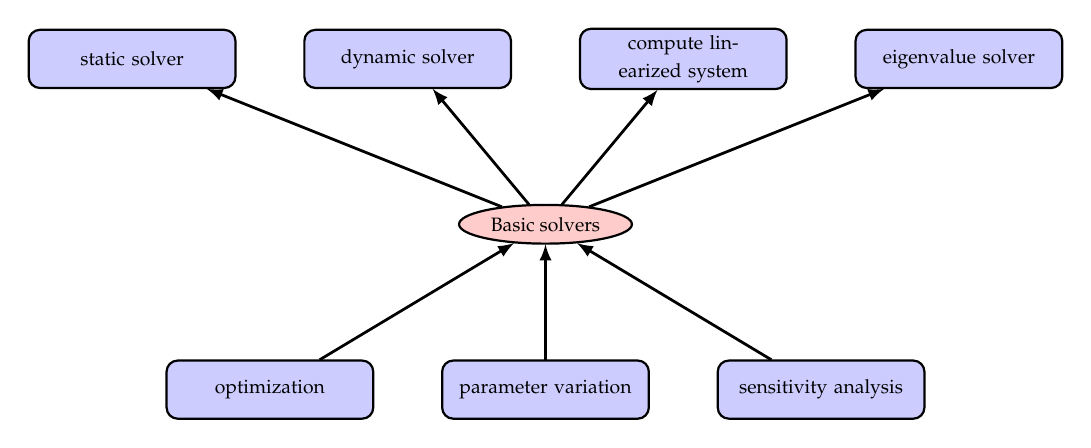
\begin{tikzpicture}[node distance = 2cm, auto, thick,scale=0.7, every node/.style={scale=0.7}]
    % Place nodes
    \node [wideblock] (solveStatic) {static solver};
    \node [wideblock, right of=solveStatic, node distance=5cm] (solveDynamic) {dynamic solver};
    \node [wideblock, right of=solveDynamic, node distance=5cm] (computeLinearized) {compute linearized system};
    \node [wideblock, right of=computeLinearized, node distance=5cm] (computeEWP) {eigenvalue solver};
%      
    \node [cloud, below of=solveDynamic, node distance=3cm, xshift = 2.5cm] (basicSolvers) {Basic solvers};
    \node [wideblock, below of=basicSolvers, node distance=3cm] (parameterVariation) {parameter variation};
    \node [wideblock, left of=parameterVariation, node distance=5cm] (optimization) {optimization};
    \node [wideblock, right of=parameterVariation, node distance=5cm] (sensitivityAnalysis) {sensitivity analysis};
    \path [arrow] (basicSolvers) -- (solveDynamic);
    \path [arrow] (basicSolvers) -- (solveStatic);
    \path [arrow] (basicSolvers) -- (computeLinearized);
    \path [arrow] (basicSolvers) -- (computeEWP);

    \path [arrow] (parameterVariation) -- (basicSolvers);
    \path [arrow] (optimization) -- (basicSolvers);
    \path [arrow] (sensitivityAnalysis) -- (basicSolvers);
  \end{tikzpicture}
  \caption{Basic and advanced solvers in \codeName\ ; advanced solvers build upon any basic solver to perform more sophisticated operations}
  \label{fig_available_solvers}
\end{figure}}
%++++++++++++++++++++++++++++++++++++++++++++++++++++++++++++++++++++++++
There are advanced solvers, like in \texttt{exudyn.processing}:
\bi
  \item \mybold{Optimization}:
  \bi
    \item \texttt{GeneticOptimization(...)}: find optimum for given set of parameter ranges using genetic optimization; works in parallel
    \item \texttt{Minimize(...)}: find optimum with \texttt{scipy.optimize.minimize(...)}
  \ei
\ei
\bi
  \item \texttt{ParameterVariation(...)}: compute a series of simulations for given set(s) of parameters; works in parallel
  \item \texttt{ComputeSensitivities(...)}: compute sensitivities for certain parameters; works in parallel
\ei
The advanced methods are build upon the basic solvers and essentially run single simulations in the background, see the according examples.

The basic solvers need a \texttt{MainSystem}, usually denoted as \texttt{mbs}, to be solved. Furthermore, a couple of options are usually to be given, which are explained shortly:
\bi
  \item \texttt{simulationSettings}: This is a big structure, containing all solver options; note that only the according options for \texttt{staticSolver} or \texttt{timeIntegration} are used. Look at the detailed description of these options in \refSection{sec:settingsStructures}. These settings influence the output rate and output quantity of the solution, solver reporting, accuracy, solver type, etc. Specifically, the \texttt{verboseMode} may be increased (2-4) to see the behavior of the solver and intermediate quantities.
  \item \texttt{solverType}: Only for \texttt{exudyn.SolveDynamic(...)}: This is a simpler access to the solverType given in the internal structure of 
  \bi
  \item[] \texttt{timeIntegration.generalizedAlpha} and 
  \item[] \texttt{simulationSettings.timeIntegration.explicitIntegration.dynamicSolverType}.
  \ei
\ei
The function \texttt{exudyn.SolveDynamic(...)} sets the according variables internally. For available solver types, see the description of \texttt{exudyn.DynamicSolverType} in \refSection{sec:DynamicSolverType}.
\bi
  \item \texttt{storeSolver}: if \texttt{True}, the solver is stored in \texttt{mbs.sys['staticSolver']} or \texttt{mbs.sys['dynamicSolver']} and also solver settings are stored in \texttt{mbs.sys['simulationSettings']}. After the solver has finished, \texttt{mbs.sys['staticSolver']} can be used to retrieve additional information on convergence, system matrices, etc. (see the solver structure).
  \item \texttt{showHints}: This shows a lot of possible solutions in case of no convergence
  \item \texttt{showCausingItems}: This shows a potential causing item if the linear solver failed; the item number is computed from the coordinate number that caused problems (e.g., a row that became zero during factorization); note that this item may not be the real cause in your problem
\ei

\mysubsubsection{System equations of motion}
The system equations of motion in \codeName\ follow the notations of \refSection{sec:nomenclatureEOM} and are represented as 
\bea \label{eq_system_EOM}
  \Mm \ddot \qv + \frac{\partial \gv}{\partial \qv^\mathrm{T}} \tlambda_q + 
                  \frac{\partial \gv}{\partial \dot \qv^\mathrm{T}} \tlambda_{\dot q}
                  & = &\fv_\SO(\qv, \dot \qv, t) \\
  \dot \yv + \frac{\partial \gv}{\partial \yv^\mathrm{T}} \tlambda & = &\fv_\FO(\yv, t) \\
  \gv(\qv, \dot \qv, \yv, \tlambda, t) &=& 0 \eqDot
\eea
Here, we introduce different Lagrange multipliers $\tlambda_q$ and $\tlambda_{\dot q}$ which have equal sizes as $\tlambda$, while those $\lambda_i$ which belong to holonomic constraints, are included in $\tlambda_q$ and $\tlambda_i$ belonging to non-holonomic constraints, are included in $\tlambda_{\dot q}$, whereas other components in $\tlambda_q$ or $\tlambda_{\dot q}$ are zero.

It may help to know that for linear mechanical the term $\fv_\SO$ becomes
\be
  \fv^{lin}_\SO = \fv_a - \Km \qv - \Dm \dot \qv
\ee
in which $\fv^a$ represents applied forces and stiffness matrix $\Km$ and damping matrix $\Dm$ become part of the system Jacobian for time integration.

\mysubsection{General solver structure}
%theory
The description of solvers in this section follows the nomenclature given in \refChapter{sec:generalnotation}.
Both in the static as well as in the dynamic case, the solvers run in a loop to solve a nonlinear system of (differential and/or algebraic) equations over a given time or load interval. Explicit solvers only perform a factorization of the mass matrix, but the \texttt{Newton} loop, see \fig{fig_solver_newton_iteration}, is replaced by an explicit computation of the time step according to a given Runge-Kutta tableau.

In case of an implicit time integration, \fig{fig_solver_time_integration} shows the basic loops for the solution process. The inner loops are shown in \fig{fig_solver_solve_steps} and\fig{fig_solver_discontinuous_iteration}.
The static solver behaves very similar, while no velocities or accelerations need to be solved and time is replaced by load steps.

Settings for the solver substructures, like timer, output, iterations, etc.\, are described in Sections \ref{sec:CSolverTimer} -- \ref{sec:SolverOutputData}.
The description of interfaces for solvers starts in \refSection{sec:MainSolverStatic}.
%
%++++++++++++++++++++++++++++++++++++++++++++++++++++++++++++++++++++++++
\onlyRST{

.. _fig-solver-time-integration:
.. figure:: docs/theDoc/figures/solverTimeIntegration.png
   :width: 400

   Basic solver flow chart for SolveSystem(). This flow chart is the same for static solver and for time integration.

}
\ignoreRST{
\begin{figure}[hb]
  \centering
  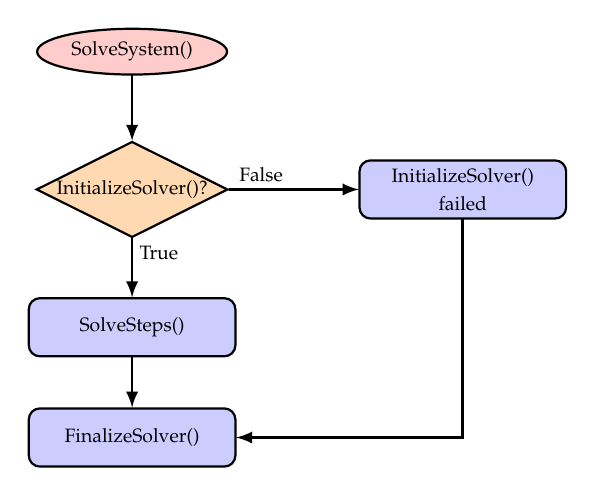
\begin{tikzpicture}[node distance = 2cm, auto, thick,scale=0.7, every node/.style={scale=0.7}]
    % Place nodes
    \node [cloud] (solveSystem) {SolveSystem()};
%    \node [wideblock, below of=init_solver_specific] (initializeSolver) {InitializeSolver()};
    \node [decision, below of=solveSystem] (decisionInitSolver) {InitializeSolver()?};
    \node [wideblock, right of=decisionInitSolver, node distance=6cm] (initFailed) {InitializeSolver() failed};
    \node [wideblock, below of=decisionInitSolver, node distance=2.5cm] (solveSteps) {SolveSteps()};
    \node [wideblock, below of=solveSteps] (finalizeSolver) {FinalizeSolver()};
    
    \path [arrow] (solveSystem) -- (decisionInitSolver);
    \path [arrow] (decisionInitSolver) -- node [near start] {False}(initFailed);
    \path [arrow] (decisionInitSolver) -- node [near start] {True}(solveSteps);
    \path [arrow] (solveSteps) -- (finalizeSolver);
    \path [arrow] (initFailed) |- (finalizeSolver);
  \end{tikzpicture}
  \caption{Basic solver flow chart for SolveSystem(). This flow chart is the same for static solver and for time integration.}
  \label{fig_solver_time_integration}
\end{figure}
}
%++++++++++++++++++++++++++++++++++++++++++++++++++++++++++++++++++++++++
\onlyRST{

.. _fig-solver-initialize-solver:
.. figure:: docs/theDoc/figures/solverInitializeSolver.png
   :width: 400

   Basic solver flow chart for function InitializeSolver().

}
\ignoreRST{
\begin{figure}[tbp]
  \centering
  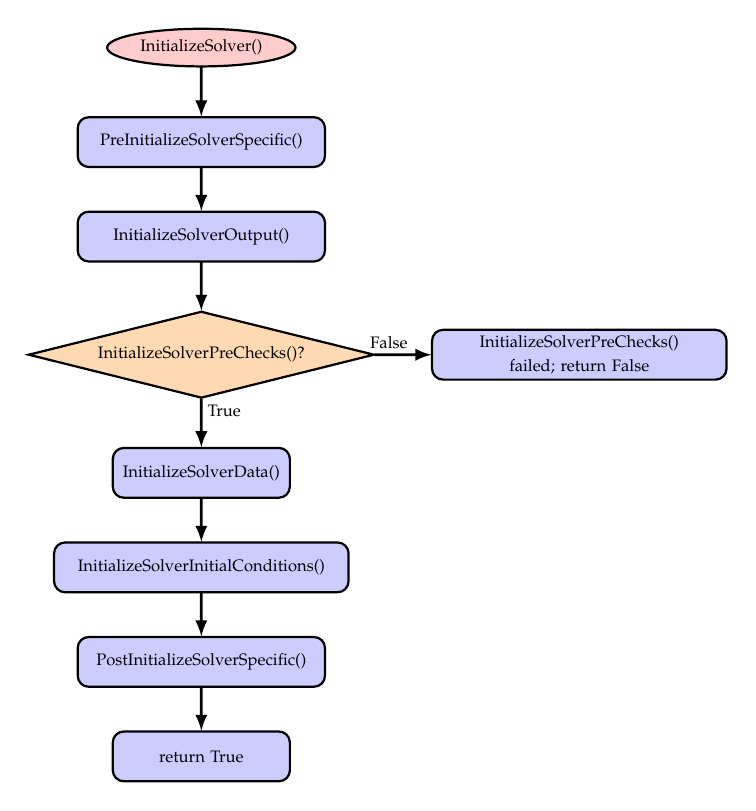
\begin{tikzpicture}[node distance = 2cm, auto, thick,scale=0.6, every node/.style={scale=0.6}]
    % Place nodes
    \node [cloud] (initializeSolver) {InitializeSolver()};
    \node [wideblock, text width=5cm, below of=initializeSolver] (preInitializeSolverSpecific) {PreInitializeSolverSpecific()};
    \node [wideblock, text width=5cm, below of=preInitializeSolverSpecific] (initializeSolverOutput) {InitializeSolverOutput()};
    \node [decision, aspect=4, text width=6cm, below of=initializeSolverOutput] (initializeSolverPreChecks) {InitializeSolverPreChecks()?};
    
    \node [wideblock, text width=6cm, right of=initializeSolverPreChecks, node distance=8cm] (initFailed) {InitializeSolverPreChecks() failed; return False};
    \node [wideblock, below of=initializeSolverPreChecks, node distance=2.5cm] (initializeSolverData) {InitializeSolverData()};
    \node [wideblock, text width=6cm, below of=initializeSolverData] (initializeSolverInitialConditions) {InitializeSolverInitialConditions()};
    \node [wideblock, text width=5cm, below of=initializeSolverInitialConditions] (postInitializeSolverSpecific) {PostInitializeSolverSpecific()};
    \node [wideblock, below of=postInitializeSolverSpecific] (finished) {return True};
    
    \path [arrow] (initializeSolver) -- (preInitializeSolverSpecific);
    \path [arrow] (preInitializeSolverSpecific) -- (initializeSolverOutput);
    \path [arrow] (initializeSolverOutput) -- (initializeSolverPreChecks);
    \path [arrow] (initializeSolverPreChecks) -- node [near start] {False}(initFailed);
    \path [arrow] (initializeSolverPreChecks) -- node [near start] {True}(initializeSolverData);
    \path [arrow] (initializeSolverData) -- (initializeSolverInitialConditions);
    \path [arrow] (initializeSolverInitialConditions) -- (postInitializeSolverSpecific);
    \path [arrow] (postInitializeSolverSpecific) -- (finished);
  \end{tikzpicture}
  \caption{Basic solver flow chart for function InitializeSolver().}
  \label{fig_solver_initialize_solver}
\end{figure}
}
%++++++++++++++++++++++++++++++++++++++++++++++++++++++++++++++++++++++++
\onlyRST{

.. _fig-solver-solve-steps:
.. figure:: docs/theDoc/figures/solverSolveSteps.png
   :width: 400

   Flow chart for SolveSteps(), which is the inner loop of the solver.

}
\ignoreRST{
\begin{figure}[tbp]
  \centering
  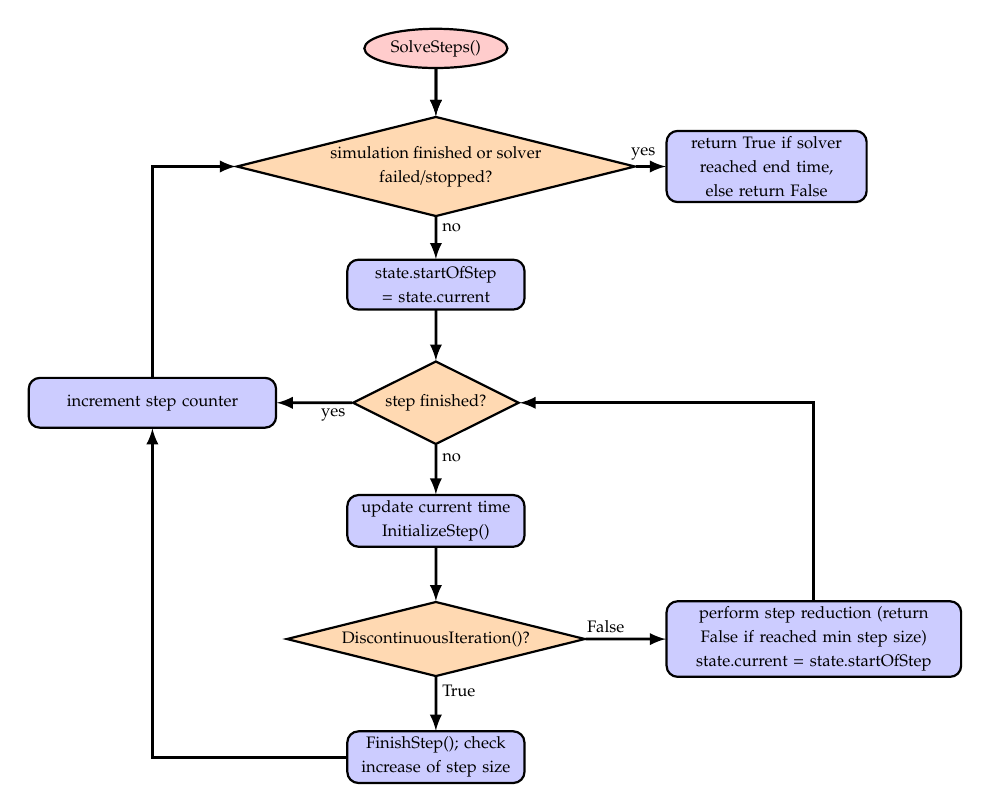
\begin{tikzpicture}[node distance = 2cm, auto, thick,scale=0.6, every node/.style={scale=0.6}]
    % Place nodes
    \node [cloud] (solveSteps) {SolveSteps()};
    \node [decision, aspect=4, text width=5cm, below of=solveSteps] (solveStepsLoop) {simulation finished or solver failed/stopped?};
    
    \node [wideblock, text width=4cm, right of=solveStepsLoop, node distance=7cm] (solveStepsLoopFinished) {return True if solver reached end time, else return False};
    \node [wideblock, below of=solveStepsLoop, node distance=2.5cm] (setStartOfStepState) {state.startOfStep = state.current};
    \node [decision, below of=setStartOfStepState] (stepReduction) {step finished?};
    \node [wideblock, text width=5cm, left of=stepReduction, node distance=6cm] (finishStep) {increment step counter};
    \node [wideblock, below of=stepReduction, yshift = -0.5cm] (initializeStep) {update current time\\InitializeStep()};
    \node [decision, aspect=4, text width=5cm, below of=initializeStep] (discontinuousIteration) {DiscontinuousIteration()?};
    \node [wideblock, text width=6cm, right of=discontinuousIteration, node distance=8cm] (discontinuousIterationFailed) {perform step reduction (return False if reached min step size)\\state.current = state.startOfStep};
    \node [wideblock, below of=discontinuousIteration, node distance=2.5cm] (finishDiscIt) {FinishStep(); check increase of step size};
    
    \path [arrow] (solveSteps) -- (solveStepsLoop);
    \path [arrow] (solveStepsLoop) -- node [near start] {no}(setStartOfStepState);
    \path [arrow] (solveStepsLoop) -- node [near start] {yes}(solveStepsLoopFinished);
    \path [arrow] (setStartOfStepState) -- (stepReduction);
    \path [arrow] (stepReduction) -- node [near start] {no}(initializeStep);
    \path [arrow] (stepReduction) -- node [near start] {yes}(finishStep);
    \path [arrow] (finishStep) |- (solveStepsLoop);
      
      \path [arrow] (initializeStep) -- (discontinuousIteration);
      \path [arrow] (discontinuousIteration) -- node [near start] {False}(discontinuousIterationFailed);
      \path [arrow] (discontinuousIteration) -- node [near start] {True}(finishDiscIt);
      \path [arrow] (solveSteps) -- (solveStepsLoop);
      \path [arrow] (discontinuousIterationFailed) |- (stepReduction);
      \path [arrow] (finishDiscIt) -| (finishStep);
  \end{tikzpicture}
  \caption{Flow chart for SolveSteps(), which is the inner loop of the solver.}
  \label{fig_solver_solve_steps}
\end{figure}
}
%++++++++++++++++++++++++++++++++++++++++++++++++++++++++++++++++++++++++
\onlyRST{

.. _fig-solver-discontinuous-iteration:
.. figure:: docs/theDoc/figures/solverDiscontinuousIteration.png
   :width: 400

   Solver flow chart for DiscontinuousIteration(), which is run for every solved step inside the static/dynamic solvers. If the DiscontinuousIteration() returns False, SolveSteps() will try to reduce the step size.

}
\ignoreRST{
\begin{figure}[tbp]
  \centering
  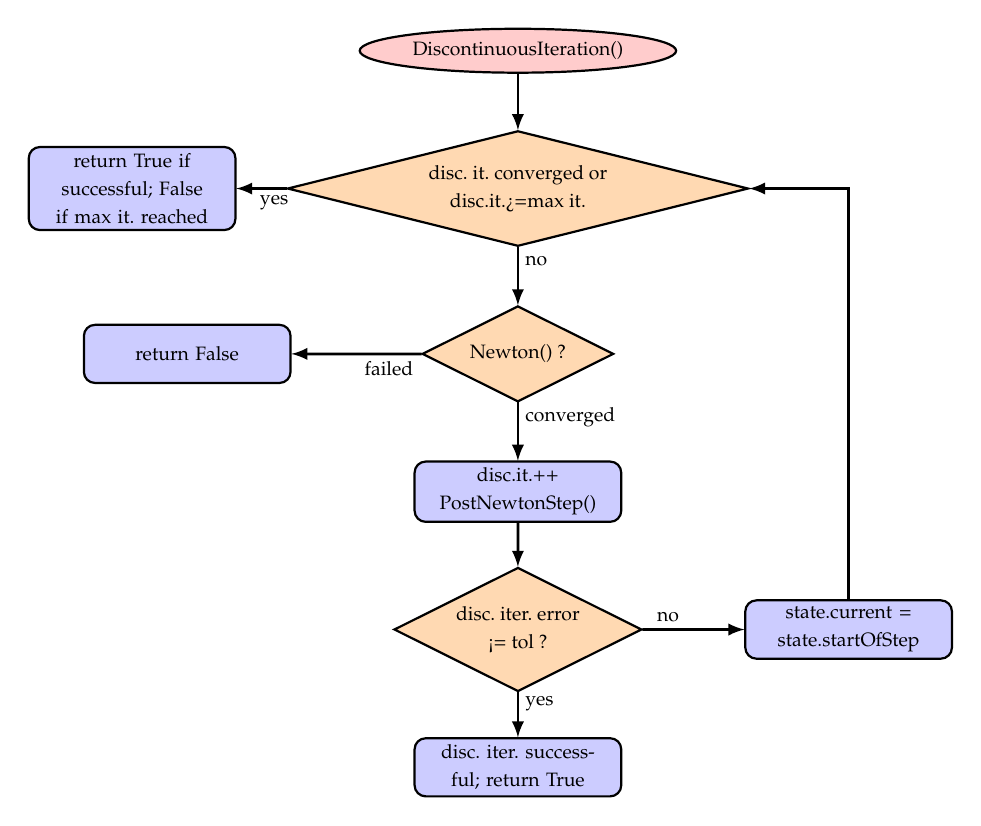
\begin{tikzpicture}[node distance = 2cm, auto, thick,scale=0.7, every node/.style={scale=0.7}]
      % Place nodes
      \node [cloud] (discontinuousIteration) {DiscontinuousIteration()};
      \node [decision, aspect=4, text width=5cm, below of=discontinuousIteration] (discontinuousIterationLoop) {disc.\ it.\ converged or disc.it.>=max it.};
      \node [wideblock, left of=discontinuousIterationLoop, node distance=6cm, xshift=-1cm] (discItTerminate) {return True if successful; False if max it.\ reached};
     
      \node [decision, below of=discontinuousIterationLoop, yshift = -0.5cm] (newtonLoop) {Newton() ?};
      \node [wideblock, left of=newtonLoop, node distance=6cm] (newtonFailed) {return False};
      \node [wideblock, below of=newtonLoop, yshift = -0.5cm] (postNewtonStep) {disc.it.++\\PostNewtonStep()};

      \node [decision, below of=postNewtonStep] (postNewtonStepError) {disc.\ iter.\ error\\ <= tol ?};
      \node [wideblock, right of=postNewtonStepError, node distance=6cm] (resetDiscIt) {state.current = state.startOfStep};
      \node [wideblock, below of=postNewtonStepError, yshift = -0.5cm] (discItSuccessful) {disc.\ iter.\ successful; return True};
      
      \path [arrow] (discontinuousIteration) -- (discontinuousIterationLoop);
      \path [arrow] (discontinuousIterationLoop) -- node [near start] {no}(newtonLoop);
      \path [arrow] (discontinuousIterationLoop) -- node [near start] {yes}(discItTerminate);
      
      %\path [arrow] (discontinuousIterationLoop) -- (newtonLoop);
      \path [arrow] (newtonLoop) -- node [near start] {failed}(newtonFailed);
      \path [arrow] (newtonLoop) -- node [near start] {converged}(postNewtonStep);

      \path [arrow] (postNewtonStep) -- (postNewtonStepError);
      \path [arrow] (postNewtonStepError) -- node [near start] {no}(resetDiscIt);
      \path [arrow] (postNewtonStepError) -- node [near start] {yes}(discItSuccessful);

      \path [arrow] (resetDiscIt) |- (discontinuousIterationLoop);
  \end{tikzpicture}
  \caption{Solver flow chart for DiscontinuousIteration(), which is run for every solved step inside the static/dynamic solvers. If the DiscontinuousIteration() returns False, 
  SolveSteps() will try to reduce the step size.}
  \label{fig_solver_discontinuous_iteration}
\end{figure}
}
%++++++++++++++++++++++++++++++++++++++++++++++++++++++++++++++++++++++++
\onlyRST{

.. _fig-solver-newton-iteration:
.. figure:: docs/theDoc/figures/solverNewton.png
   :width: 320

   Solver flow chart for Newton(), which is run inside the DiscontinuousIteration(). The shown case is valid for newtonResidualMode = 0.

}
\ignoreRST{
\begin{figure}[tbp]
  \centering
  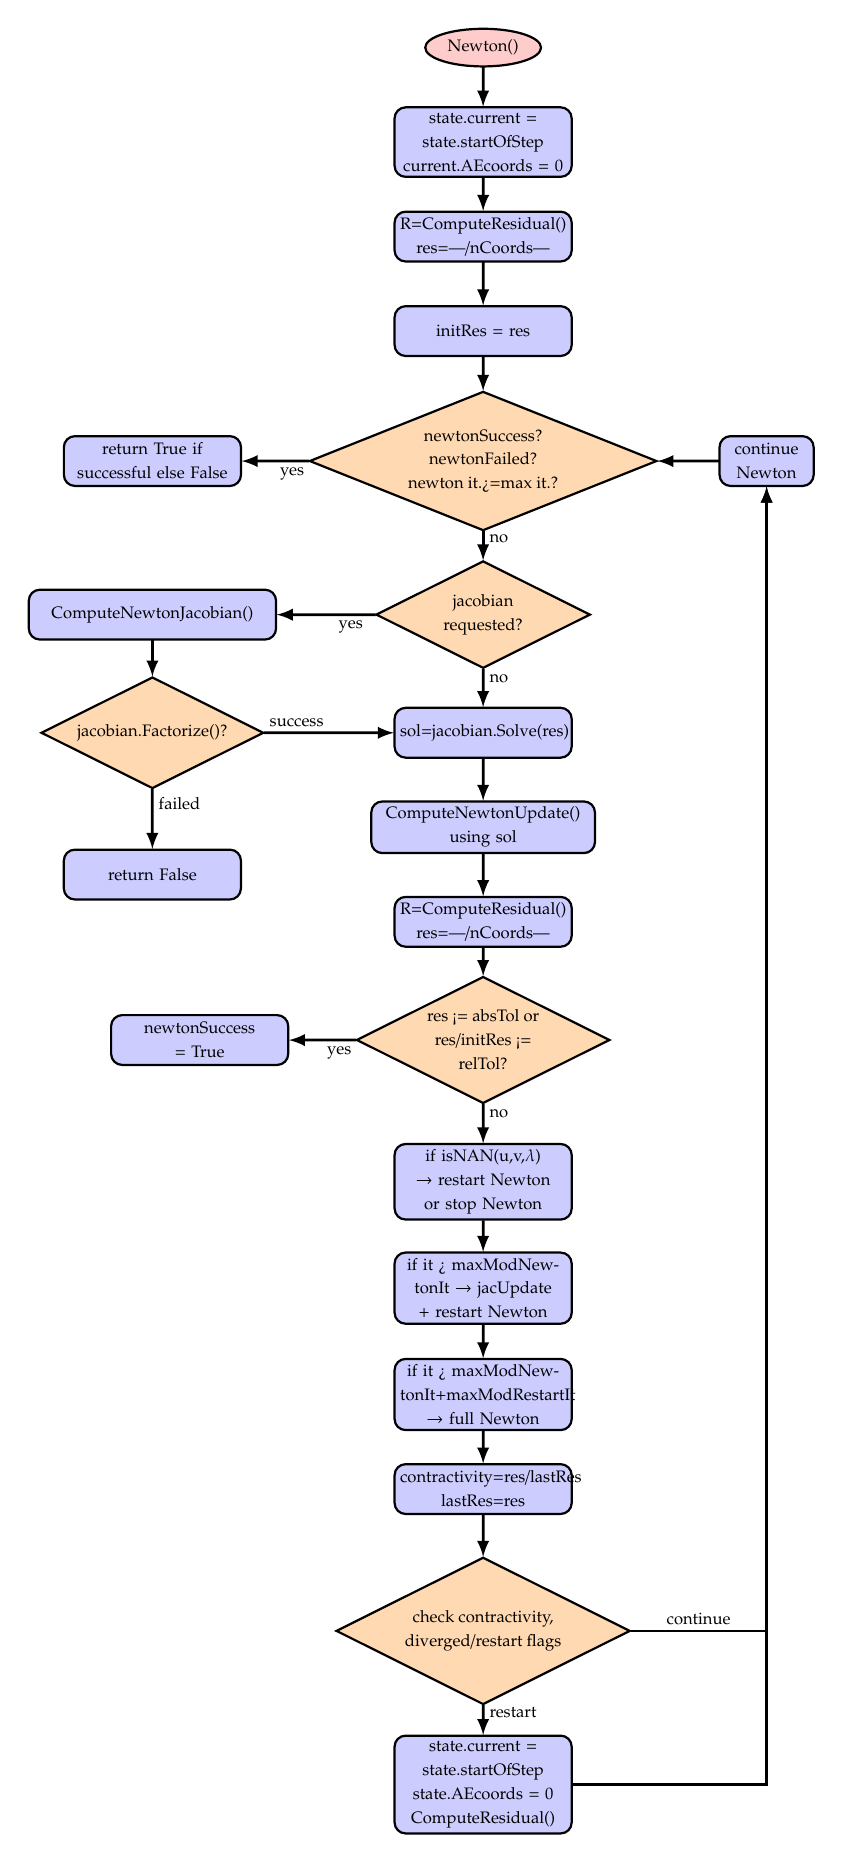
\begin{tikzpicture}[node distance = 2cm, auto, thick,scale=0.6, every node/.style={scale=0.6}]
      % Place nodes
      \node [cloud] (newtonIteration) {Newton()};
      \node [wideblock, below of=newtonIteration] (initNewton) {state.current = state.startOfStep\\ current.AEcoords = 0};
      \node [wideblock, below of=initNewton] (residual) {R=ComputeResidual()\\res=|/nCoords|};
      \node [wideblock, below of=residual] (initResidual) {initRes = res};

      \node [decision, aspect=2.5, text width=4cm, below of=initResidual, yshift = -0.25cm] (newtonLoop) {newtonSuccess?\\newtonFailed?\\newton it.>=max it.?};
      \node [wideblock, left of=newtonLoop, node distance=6cm, xshift=-1cm] (newtonTerminate) {return True if successful else False};
      \node [block, right of=newtonLoop, node distance=6cm] (continueNewton) {continue Newton};
      \node [decision, below of=newtonLoop, yshift = -0.75cm] (jacUpdate) {jacobian requested?};

      \node [wideblock, text width = 5cm, left of=jacUpdate, node distance=7cm] (updateJacobian) {ComputeNewtonJacobian()};
      \node [decision, text width = 4cm, below of=updateJacobian, yshift = -0.0cm] (factorizeJacobian) {jacobian.Factorize()?};
      \node [wideblock, below of=factorizeJacobian, yshift = -1.0cm] (jacFactorizeFailed) {return False};

      \node [wideblock, below of=jacUpdate, yshift = -0.5cm] (jacobianSolve) {sol=jacobian.Solve(res)};
      \node [wideblock, below of=jacobianSolve, text width=4.5cm, yshift = -0.0cm] (newtonUpdate) {ComputeNewtonUpdate() using sol};
      \node [wideblock, below of=newtonUpdate] (residual2) {R=ComputeResidual()\\res=|/nCoords|};

      %\node [wideblock, below of=residual2] (adaptInitResidual) {initResidual = max(res,initRes)};
      \node [decision, below of=residual2] (evalTolerances) {res <= absTol or res/initRes <= relTol?};
      \node [wideblock, left of=evalTolerances, node distance=6cm] (newtonConverged) {newtonSuccess = True};
      \node [wideblock, below of=evalTolerances, yshift=-1cm] (checkDivergence) {if isNAN(u,v,$\lambda$)\\ $\ra$ restart Newton or stop Newton};
      \node [wideblock, below of=checkDivergence, yshift=-0.25cm] (checkIterations) {if it > maxModNewtonIt $\ra$ jacUpdate + restart Newton};
      \node [wideblock, below of=checkIterations, yshift=-0.25cm] (checkIterations2) {if it > maxModNewtonIt+maxModRestartIt $\ra$ full Newton};
      \node [wideblock, below of=checkIterations2, yshift=-0.cm] (checkContractivity) {contractivity=res/lastRes\\lastRes=res};
      \node [decision, text width=4.5cm, below of=checkContractivity, yshift=-0.5cm] (restartNewton) {check contractivity, diverged/restart flags};
      
      \node [wideblock, below of=restartNewton, yshift=-1.25cm] (restartNewtonIteration) {state.current = state.startOfStep\\ state.AEcoords = 0\\ComputeResidual()};
  
      \path [arrow] (newtonIteration) -- (initNewton);
      \path [arrow] (initNewton) -- (residual);
      \path [arrow] (residual) -- (initResidual);

      \path [arrow] (initResidual) -- (newtonLoop);
      \path [arrow] (newtonLoop) -- node [near start] {no}(jacUpdate);
      \path [arrow] (newtonLoop) -- node [near start] {yes}(newtonTerminate);
      %
      \path [arrow] (jacUpdate) -- node [near start] {no}(jacobianSolve);
      \path [arrow] (jacUpdate) -- node [near start] {yes}(updateJacobian);

      \path [arrow] (updateJacobian) -- (factorizeJacobian);
      \path [arrow] (factorizeJacobian) -- node [near start] {failed}(jacFactorizeFailed);
      \path [arrow] (factorizeJacobian) -- node [near start] {success}(jacobianSolve);
%
      \path [arrow] (jacobianSolve) -- (newtonUpdate);
      \path [arrow] (newtonUpdate) -- (residual2);

      \path [arrow] (residual2) -- (evalTolerances);
      \path [arrow] (evalTolerances) -- node [near start] {yes}(newtonConverged);
      \path [arrow] (evalTolerances) -- node [near start] {no}(checkDivergence);
      \path [arrow] (checkDivergence) -- (checkIterations);
      \path [arrow] (checkIterations) -- (checkIterations2);
      \path [arrow] (checkIterations2) -- (checkContractivity);
      \path [arrow] (checkContractivity) -- (restartNewton);
      \path [arrow] (restartNewton) -- node [near start] {restart}(restartNewtonIteration);
      \path [arrow] (restartNewton) -| node [near start] {continue}(continueNewton);
      \path [arrow] (restartNewtonIteration) -| (continueNewton);
      
      \path [arrow] (continueNewton) -- (newtonLoop);

  \end{tikzpicture}
  \caption{Solver flow chart for Newton(), which is run inside the DiscontinuousIteration(). The shown case is valid for newtonResidualMode = 0.}
  \label{fig_solver_newton_iteration}
\end{figure}
\clearpage
}
%
\mysubsectionlabel{Explicit solvers}{sec:ExplicitSolver}
Explicit solvers are in general only applicable for systems without constraints (i.e., no joints!). However, some solvers accept simple \texttt{CoordinateConstraint}, e.g., fixing coordinates to the ground.
Nevertheless, for constraint-free systems, e.g., with penalty constraints, can be solved for very high order and with great efficiency.
A list of explicit solvers is available, see \refSection{sec:DynamicSolverType}, for an overview of all implicit and explicit solvers.

The solution vector $\txi$ (denoted as $y$ in the literature \cite{Hairer1987}), which is defined as
\be
  \txi = [\qv\tp \;\; \dot \qv\tp \;\; \yv\tp ]\tp
\ee
and which includes \hac{ODE2} coordinates and velocities and \hac{ODE1} coordinates. All coordinates are computed without reference values.

The \hac{ODE1} and \hac{ODE2} equations of \eq{eq_systemEOM}, with $\tlambda=0$, are written in explicit form and converted to first order equations,
\bea \label{eq_systemEOM}
  \dot \qv &=& \vel \nonumber \\
  \dot \vel & = &\Mm^{-1} \fv_\SO(\qv, \vel, t) \nonumber \\
  \dot \yv & = &\fv_\FO(\yv, t) \\
\eea
The system first order differential equations for explicit solvers thus read
\be
  \dot \txi = \fv_e (\txi, t)
\ee
%
\mysubsubsectionlabel{Explicit Runge-Kutta method}{sec:rungekuttamethod}
Explicit time integration methods seek the solution $\txi_{t+h}$ at time $t+h$ for given initial value $\txi_{t}$ (at the beginning of one step $t$ or at the beginning of the simulation, $t=0$),
\be
  \txi_{t+h} = \txi_{t} + \Delta \txi\eqDot
\ee
For any given Runge-Kutta method, the integration of one step with step size $h$ is performed by an approximation
\be \label{s_stage_quadrature}
  \Delta \txi = \int _{t}^{t+h}\fv_e(\tau ,\txi(\tau ))d\tau \approx h\left[b_{1} \fv_e(t,\txi(t))+b_{2} \fv_e(t+c_{2} h,\txi(t+c_{2} h))+ \ldots +b_{s} \fv_e(t+\txi_{s} h,u(t+\txi_{s} h))\right] %  \eqref{GrindEQ__12_12_}
\ee
%
in which $t + c_{i}h$ is the time for stage $i$ and $b_i$ the according weight given in the integration formula.
Stages are within one step (therefor called one-step-methods), where $c_i=0$ represents the beginning of the step and $c_i=1$ the end.
Note that $c_{1}= 0$ for explicit integration formulas.

The unknown solution vectors $\txi$ at the stages are abbreviated by
\be
  \gv_{i} \approx \txi(t+c_{i} h) 
\ee
and computed by explicit integration (quadrature) formulas of lower order ($g_i$ not to be mixed up with algebraic equations!),
\be \label{eq_expl_RK_stages}
  \begin{array}{l} 
  {\gv_{1} =\txi_t} \\
  {\gv_{2} =\txi_t+ha_{21} \fv_e(t,\gv_{1} )} \\
  {\gv_{3} =\txi_t+h\left[a_{31} \fv_e(t,\gv_{1} )+a_{32} \fv_e(t+c_{2} h,\gv_{2} )\right]} \\
  {{\rm \; \; \; \; \; \; }\vdots } \\
  {\gv_{s} =\txi_t+h\left[a_{s1} \fv_e(t,\gv_{1} )+a_{s2} \fv_e(t+c_{2} h,\gv_{2} )+ \ldots +a_{s,s-1} \fv_e(t+c_{s-1} h,\gv_{s-1} )\right]} \end{array} 
\ee
After all vectors $\gv_i$ have been consecutively evaluated, the step is updated by \eq{s_stage_quadrature}.

\onlyRST{
For some exemplary tableaus of explicit and impliciti Runge-Kutta methods, see theDoc.pdf!
}
\ignoreRST{
Conventional explicit Runge-Kutta solvers, such as \texttt{ExplicitMidPoint}, \texttt{RK44} or \texttt{RK67} are based on 
fixed step size and users must control the error by choosing an appropriate global step size. The tableaus for some lower order methods
%\texttt{ExplicitEuler}, \texttt{ExplicitMidpoint} and \texttt{RK44} 
are given in Table \ref{tab:rungeKuttaTableaus}, using the structure
\begin{center}
\begin{tabular}{p{0.25cm}|p{0.25cm}} 
$\cv$ & $\Am$ \\ \hline 
~ & $\bv\tp$ \\ 
\end{tabular}
\end{center}
with
\begin{center}
\begin{tabular}{p{0.35cm}|p{0.35cm} p{0.35cm} p{0.35cm} p{0.35cm} } %\hline 
0 & 0 & & &\\ %\hline
$c_2$ & $a_{21}$ & $\ddots$ & & \\ %\hline
$\vdots$ & $\vdots$ & $\ddots$ & $\ddots$ & \\ %\hline
$c_s$ & $a_{s1}$ & $\cdots$ & $a_{s,s-1}$ & 0 \\ \hline
      & $b_{1}$ & $\cdots$ & $b_{s-1}$ & $b_{s}$ \\ %\hline
\end{tabular} 
\end{center}
%\be
  %\mp{\cv}{\Am}{}{\bv}, \quad \Am = \vr{a_{11}}{\cdots}{a_{1s}} {\vdots}{\cdots}{\vdots} {a_{s1}}{\cdots}{a_{ss}}
%\ee
with $\cv = [c_0=0, \; c_1, \; \ldots, \; c_s]$, $\bv = [b_0, \; b_1, \; \ldots, \; b_s]$, and $\Am$ having only entries in the 
lower left triangle.
For number of stages $s > 4$, the maximum order of explicit methods is lower than the number of stages, such as for \texttt{RK67}, which as order 6 but 7 stages.
%
\begin{table}
%
Explicit Euler method, number of stages $s=1$, order $p=1$:\\
\begin{center}
\begin{tabular}{p{0.1in}|p{0.1in}} %\hline 
0 & ~ \\ \hline 
~ & 1 \\ %\hline 
\end{tabular} \vspace{0.5cm}
\end{center}

Explicit midpoint rule, number of stages $s=2$, order $p=2$:\\
\begin{center}
\begin{tabular}{c|c c} %\hline 
0 &  &  \\ %\hline 
1/2 & 1/2 &  \\ \hline 
 & 0 & 1 \\ %\hline 
\end{tabular} \vspace{0.5cm}
\end{center}

Classical explicit Runge-Kutta method (RK44) , number of stages $s=4$, order $p=4$:\\
%\begin{tabular}{|p{0.2in}|p{0.2in}|p{0.2in}|p{0.2in}|p{0.2in}|} \hline 
\begin{center}
\begin{tabular}{c|c c c c }
0 &  &  &  &  \\ %\hline 
1/2 & 1/2 &  &  &  \\ %\hline 
1/2 & 0 & 1/2 &  &  \\ %\hline 
1 & 0 & 0 & 1 &  \\ \hline 
 & 1/6 & 1/3 & 1/3 & 1/6 \\ %\hline 
\end{tabular}
\end{center}
%
\caption{Several examples of tableaus for the implemented Runge-Kutta methods.}
\label{tab:rungeKuttaTableaus}
\end{table}
}
%
\mysubsubsection{Automatic step size control}
%
Advanced solvers, such as \texttt{ODE23} and \texttt{DOPRI5}, include automatic step size control\footnote{activated with
\texttt{timeIntegration.automaticStepSize = True} in simulationSettings}.

We estimate the error of a time step with current step size $h$ by
using an embedded Runge-Kutta formula, which includes two approximations \eqq{s_stage_quadrature} of order $p$ and $\hat p = p-1$, which is obtained by using two different integration formulas with common coefficients $c_i$, but two sets of weights $b_i$ and $\hat b_i$, leading to two approximations $\txi$ and $\hat \txi$. These so-called embedded Runge-Kutta formulas are widely used, for details see Hairer et al.\ \cite{Hairer1987}. 

The according apporximations $\txi$ and $\hat \txi$ are used to estimate an error 
\be
  e_j=|\xi_j- \hat \xi_j|
\ee
for every component $j$ of the solution vector $\txi$.
A scaling is used for every component of the solution vector, evaluating at the beginning ($0$) and end ($1$) of the time step:
\be
  s_j = a_{tol} + r_{tol} \cdot \mathrm{max}(|\xi_{0j}|, |\xi_{1j}|) 
\ee
Then the relative, scaled, scalar error for the step, which needs to fulfill $err \le 1$, is computed as 
\be
  err = \sqrt{\frac 1 n \sum_{j=1}^n \left( \frac{\xi_{1j} - \hat \xi_{1j}}{s_j} \right)^2}
\ee
The optimal step size then reads
\be
  h_{opt} = h \cdot \left(\frac{1}{err} \right)^{(1/(q+1))}
\ee
Currently we use the suggested step size as
\be
  h_{new} = \mathrm{min}\left(h_{max}, \mathrm{min}\left(h \cdot f_{maxInc},  \mathrm{max}(h_{min}, f_{sfty} \cdot h_{opt}) \right) \right)
\ee
With the maximum step size $h_{max} = \frac{t_{start} - t_{end}}{n_{steps}}$ and the minimum step size $h_{min}$, given in the \texttt{timeIntegration} 
\texttt{simulationSettings}.
The factor $f_{maxInc}$ limits the increase of the current step size $h$, the factor $f_{sfty}$ is a safety factor for limiting the chosen step size relative to the optimal one in order to avoid frequent step rejections. 
If $h_{new} \le h$, the current step is accepted, otherwise the step is recomputed with $h_{new}$.
For more details, see Hairer et al.\ \cite{Hairer1987}.

\mysubsubsection{Stability limit}
Note that there are hard limitations for every explicit integration method regarding the step size. Especially for stiff systems (basically with high stiffness parameters and small masses, but also with restrictions to damping), the \mybold{step size} $h$ \mybold{has an upper limit}: $h < h_{lim}$. Above that limit the method is inherently unstable, which needs to be considered both for constant and automatic step size selection.

\mysubsubsection{Explicit Lie group integrators}
All explicit solvers including the automatic step size solvers (DOPRI5, ODE23) have been equiped with Lie group integration functionality, see Holzinger et al.\ \cite{HolzingerArnoldGerst2023}.

Basically, the integration formulas, see \refSection{sec:rungekuttamethod} are extended for special rotation parameters.
Lie group integration is currently only available for \texttt{NodeRigidBodyRotVecLG} used in \texttt{ObjectRigidBody} (3D rigid body). 
\texttt{FFRFreducedOrder} will be extended to such nodes in the near future.
To get Lie group integrators running with rigid body models, all 3D node types need to be set to \texttt{NodeRigidBodyRotVecLG} and 
set \texttt{explicitIntegration.useLieGroupIntegration = True}.

\mysubsubsection{Constraints with explicit solvers}
Explicit solvers generally do not solve for algebraic constraints, except for very simple \texttt{CoordinateConstraint}. 
All connectors having the additional \texttt{type=Constraint}, see the according object in \refSection{sec:item:ObjectConnectorSpringDamper}ff., 
are in general not solvable by explicit solvers. 
Currently, only \texttt{CoordinateConstraint} with one coordinate fixed to ground can be accounted for, 
if \texttt{explicitIntegration.eliminateConstraints == True}. 
However, this offers the great flexibility to compute finite elements (imported meshes or ANCF beams) to be (partially) fixed to ground.
A \texttt{CoordinateConstraint} that fixes a coordinate with index $j$ to ground leads to the simple algebraic \hac{ODE2} equation
\be
  g_j(\qv) = 0 \quad \Leftrightarrow \quad  q_j = 0
\ee
which can be solved by the implemented explicit solvers by just setting $q_j = 0$ previously to every computation and $\dot q_j = 0$ after every \hac{RHS} evaluation.

NOTE that, if \texttt{explicitIntegration.eliminateConstraints == False}, constraints are ignored by the explicit solver (and all algebraic variables are set to zero). This may be wanted (e.g.\ to investigate the free motion of bodies), but in general leads to wrong and meaningless solution.

\mysubsectionlabel{Implicit trapezoidal rule-based, Newmark and Generalized-alpha solver}{sec:ImplicitTrapezoidalSolver}
This solver represents a class of solvers, which are -- in the undamped case -- based on the implicit trapezoidal rule (in the view of Runge-Kutta methods). The interpolation of the quantities for one step includes the start and the end value of the time step, thus being called trapezoidal integration rule. In some special cases in Newmark's method \cite{Newmark1959}, the interpolation might only depend on the start value or the end value.

For now, all implemented solvers can be viewed as a generalization of Newmark's method, but there are called differently in the solver interfaces
\bi
  \item \mybold{Implicit trapezoidal rule} (Newmark with $\beta = \frac 1 4$ and $\gamma = \frac 1 2$) 
  \item \mybold{Newmark's method} \cite{Newmark1959}
  \item \mybold{Generalized}-$\alpha$ \mybold{method} ($=$ generalized Newmark method with additional parameters), see Chung and Hulbert \cite{Chung1993} for the original method and Arnold and Br\"uls \cite{Arnold2007} for the application to multibody system dynamics.
\ei

\mysubsubsection{Newmark and Generalized-alpha method}
Newmark's method has two parameters $\beta$ and $\gamma$. 
The main ideas are given in the following.
First, displacements and velocities are linearly interpolated using the accelerations $\ddot \qv$ of the beginning of the time step (subindex '0') and the end of the time step (subindex 'T'). 
The \SON\ displacements and velocities and for \FON\ coordinates are given by (definition of $\aalg$ will become clear later):
\bea \label{eq_Newmark_interpolation}
  \qv_T & = &      \qv_0 + h \dot \qv_0 + h^2 (\frac 1 2 -\beta) \aalg_0 + h^2 \beta \aalg_T \nonumber\\  
  \dot \qv_T & = & \dot \qv_0 + h (1-\gamma) \aalg_0 + h\gamma \aalg_T \nonumber\\
  \yv_T & = & \yv_0 + h (1-\gamma_\FO) \vel^0_\FO + h\gamma_\FO \vel^T_\FO
\eea
Hereafter, the system equations are solved at the end of the time step ($T$) for the unknown accelerations as well as for \FON\ and \AEN\ coordinates.

\noindent Remarks:
\bi
  \item The system of equations may be solved for accelerations $\ddot \qv$, but also for displacements $\qv$ or even velocities as unknowns while the remaining quantities are reconstructed from \eq{eq_Newmark_interpolation}. In case of displacements as unknowns, a scaling of the Jacobian is necessary, see later.
  \item For consistency reasons, one may set $\gamma_\FO = \gamma$, but \mybold{currently we use} $\gamma_T = \frac 1 2$, leading to no numerical damping for \hac{ODE1} variables $\yv$.
  \item In the extension to the so-called generalized-$\alpha$ method \cite{Chung1993}, algorithmic accelerations $\aalg$ are used in \eq{eq_Newmark_interpolation}. 
  \item Algorithmic accelerations are no longer equivalent to the time derivatives of displacements, $\aalg \neq \ddot \qv$; thus, both sets of variables are used independently. In case of Newmark or the implicit trapezoidal rule just use $\aalg = \ddot \qv$.
  \item Implicit solvers are also available with Lie groups, if according rigid body nodes (\texttt{NodeRigidBodyRotVecLG}) are used, for theory see Holzinger et al.\ \cite{HolzingerArnoldGerst2023}.
\ei
%
For generalized-$\alpha$, the algorithmic accelerations $\aalg$ are computed from the recurrence relation
\be
   (1-\alpha_m)\av_T + \alpha_m \av_0 = (1-\alpha_f) \ddot \uv_T + \alpha_f \ddot \uv_0
\ee
which can be resolved for the unknown $\av_T$,
\be
  \av_T = \frac{(1-\alpha_f) \ddot \uv_T + \alpha_f \ddot \uv_0 - \alpha_m \av_0}{(1-\alpha_m)}
\ee
For the first step, one can simply use $\aalg_0 = \ddot \qv_0$.
%
\mysubsubsectionlabel{Parameter selection for Generalized-alpha}{sec:parametersGeneralizedAlpha}
Compared to alternative implicit integration methods (including the Newmark method), the generalized-$\alpha$ integrator's parameters break down to one single parameter $\rho_\infty$, which allows to chose numerical damping in a practical way.

Based on a simple single DOF mass-spring-damper model \cite{Bauchau2011}, having the eigen frequency $\omega = 2\pi f$ with frequency $f$ and period $T=1/f$, the spectral radius $\rho$ for the integrator defines the amount of damping for a given step size $h$ related to $T$, thus using the dimensionless step size $\bar h=h/T$.

In \fig{fig:spectralRadius} the spectral radius is shown versus $\bar h$ for various spectral radii at infinity $\rho_\infty$. 
Here, $\rho_\infty$ specifies the numerical damping of very time step for large step sizes (or very high frequencies). An amount of $\rho_\infty=0.9$ means that high frequency parts of the system (($\bar h \gg 1$); high compared to the step rate) are damped to $90\%$ in every step, reducing an initial value $1$ to $2.66e-5$ after 100 steps, which is already much larger than usual physical damping in many cases.

Furthermore, low frequency parts of the system ($\bar h \ll 1$) receive almost no numerical damping, see again \fig{fig:spectralRadius}. 
Exemplarily, consider $\rho$ a low frequency situation with different $\rho_\infty$:
\bi
  \item $\rho(\bar h=0.01, \rho_\infty=0.9) = 1 - 1.13\cdot 10^{-9}$
  \item $\rho(\bar h=0.01, \rho_\infty=0.6) = 1 - 1.22\cdot 10^{-7}$
\ei
which shows that numerical damping is very low for moderately small step sizes (100 steps for one oscillation).

Obviously, $\rho_\infty$ does not have a large influence for very high or low frequencies in the system as long as it is $\neq 1$ and we could even use $\rho_\infty=0$.
Regarding differential algebraic equations (DAEs), $\rho_\infty<1$ allows to integrate index 3 DAEs. Typically a value of $\rho_\infty=0.7$ leads to a stable integration, but values depend on the structure of the multibody system.

Once having chosen $\rho_\infty$, all other parameters follow automatically \cite{Chung1993}, regarding the $\alpha$s
\be
  \alpha_m = \frac{2 \rho_\infty - 1}{\rho_\infty + 1}, \quad
  \alpha_f = \frac{\rho_\infty}{\rho_\infty + 1}
\ee
and Newmarks's parameters,
\be
  \gamma = \frac{1}{2} - \alpha_m + \alpha_f, \quad 
  \beta = \frac{1}{4}(1- \alpha_m + \alpha_f)^2
\ee

\LatexRSTfigure{figures/spectralRadiusZeta0}{fig:spectralRadius}{9cm}{400}{Spectral radius for generalized-$\alpha$ method depending on dimensionless step size $\bar h=h/T$, in which $T$ is the period of an equivalent single DOF mass-spring-damper system.}
%\begin{figure}[tbh]%
%\begin{center}
%\includegraphics[width=0.6\columnwidth]{figures/spectralRadiusZeta0}%
%\end{center}
%\caption{Spectral radius for generalized-$\alpha$ method depending on dimensionless step size $\bar h=h/T$, in which
%$T$ is the period of an equivalent single DOF mass-spring-damper system.}%
%\label{fig:spectralRadius}%
%\end{figure}


% ++++++++++++++++++++++++++++++++++++++++++++++++++++++++
% ++++++++++++++++++++++++++++++++++++++++++++++++++++++++
\mysubsubsection{Newton iteration}
%
Thus, the residuals at the end of the time step ($T$) read (put all terms to \hac{LHS}):
\bea \label{eq_generalizedAlphaRes}
  \rv^\GA_\SO &=& \Mm \ddot \qv_T + \frac{\partial \gv}{\partial \qv^\mathrm{T}} \tlambda_T - \fv_\SO(\qv_T, \dot \qv_T, t) = 0\\
  \rv^\GA_\FO &=& \dot \yv_T + \frac{\partial \gv}{\partial \yv^\mathrm{T}} \tlambda_T - \fv_\FO(\yv_T, t) = 0\\
  \rv^\GA_\AE &=& \gv(\qv_T, \dot \qv_T, \yv_T, \tlambda_T, t) = 0
\eea
%
We consider two options for \SON: (A) solve for unknown accelerations $\acc_T$,  or (B) for unknown displacements $\qv_T$.

\mysubsubsubsection{(A) Solve for unknown accelerations}
%
The unknowns for the Newton method then are
\be \label{eq_Newton_unknowns1}
  \txi^\GA_{k+1} = \vr{\acc_T}{\yv_T}{\tlambda_T}
\ee
and at the beginning of the step, we have
\be \label{eq_Newton_unknowns2}
  \txi^\GA_{k} = \vr{\acc_0}{\yv_0}{\tlambda_0}
\ee
For the Newton method, we need to compute an update for the unknowns of \eq{eq_Newton_unknowns1}, using the previous residual $\rv_{k}$ and the inverse of the Jacobian $\Jm_{k}$ of Newton iteration $k$,
\be
  \txi^\GA_{k+1} = \txi^\GA_{k} - \Jm^{-1} \left( \txi^\GA_{k} \right) \cdot \rv^\GA \left( \txi^\GA_{k} \right)
\ee

% +++++++++++++++++++++
% Jacobians for Newmark
The Jacobian has the following $3 \times 3$ structure,
\be
  \Jm = \mr{\Jm_{\SO\SO}}{\Jm_{\SO\FO}}{\Jm_{\SO\AE}}
           {\Jm_{\FO\SO}}{\Jm_{\FO\FO}}{\Jm_{\FO\AE}}
           {\Jm_{\AE\SO}}{\Jm_{\AE\FO}}{\Jm_{\AE\AE}}
      = \mr{\Jm_{\SO\SO}}{\Null}{\Jm_{\SO\AE}}
           {\Null}{\Jm_{\FO\FO}}{\Jm_{\FO\AE}}
           {\Jm_{\AE\SO}}{\Jm_{\AE\FO}}{\Jm_{\AE\AE}}
\ee
in which we consider $\Jm_{\FO\SO}$ and $\Jm_{\SO\FO}$ to vanish in the current implementations, which means that coupling of \hac{ODE1} and \hac{ODE2} coordinates is only possible due to algebraic equations.

The remaining terms in the Jacobian are currently (or by default settings) evaluated as:
\bea
  \Jm_{\SO\SO}&=&\frac{\partial \rv^\GA_\SO}{\partial \acc} 
               = \frac{\partial \rv^\GA_\SO}{\partial \qv} \frac{\partial \qv}{\partial \acc} 
                 + \frac{\partial \rv^\GA_\SO}{\partial \dot \qv} \frac{\partial \dot \qv}{\partial \acc} 
               = h^2 \beta \Km + h \gamma \Dm
               \nonumber \\
  \Jm_{\SO\AE}&=&\frac{\partial \rv^\GA_\SO}{\partial \tlambda} 
               = \frac{\partial \gv}{\partial \qv} \quad (\mbox{or } \frac{\partial \gv}{\partial \dot \qv} \mbox{ for constraints at velocity level)} \nonumber \\
  \Jm_{\FO\FO}&=&\frac{\partial \rv^\GA_\FO}{\partial \yv} \nonumber \\
  \Jm_{\AE\SO}&=&\frac{\partial \rv^\GA_\AE}{\partial \acc}
               = \frac{\partial \gv}{\partial \acc}
               = \frac{\partial \gv}{\partial \qv} \frac{\partial \qv}{\partial \acc} + 
                 \frac{\partial \gv}{\partial \dot \qv} \frac{\partial \dot \qv}{\partial \acc}
               = h^2 \beta \frac{\partial \gv}{\partial \qv} 
                 + h \gamma \frac{\partial \gv}{\partial \dot \qv}
              \nonumber \\
  \Jm_{\AE\FO}&=&\frac{\partial \rv^\GA_\AE}{\partial \yv} \nonumber \\
  \Jm_{\AE\AE}&=&\frac{\partial \rv^\GA_\AE}{\partial \tlambda}
               = \frac{\partial \gv}{\partial \tlambda}
\eea
Note that some parts of the Jacobian are \mybold{neglected}, such as mass matrix and constraint Jacobian terms in $\Jm_{\SO\SO}$, which are usually of minor influence. Furthermore, Jacobians for state-dependent loads are neglected except for system-wide numerical Jacobians or if \texttt{computeLoadsJacobian} in static or time integration solvers is set True.

Once an update $\qv^\mathrm{Newton}_{k+1}$ has been computed, the interpolation formulas \eqref{eq_Newmark_interpolation} need to be evaluated before the next residual and Jacobian can be computed.
%
\mysubsubsubsection{(B) Solve for unknown displacements}
%
This approach is similar to the previous approach and follows exactly the algorithm given by Arnold and Br\"uls \cite{Arnold2007}, however, extended for \hac{ODE1} variables, which are integrated by the (undamped) trapezoidal rule.
Documentation will be added lateron.

\mysubsubsection{Initial accelerations}
%
For the solvers based on the implicit trapezoidal rule, initial accelerations are necessary in order to significantly increase the accuracy
of the first time step.
For this reason, the constraints $\gv(\qv_0, \dot \qv_0, \yv_0, \tlambda_0, t) = 0$ in \eq{eq_system_EOM} are differentiated w.r.t.\ time,
\be \label{eq_initialAccelerationsVel}
  \dot \gv(\qv_0, \dot \qv_0, \yv_0, \tlambda_0, t) = 
  \frac{\partial \gv}{\partial \qv} \dot \qv_0 + 
  \frac{\partial \gv}{\partial \dot \qv}\ddot \qv_0 +
  \frac{\partial \gv}{\partial \yv} \dot \yv_0 + 
  \frac{\partial \gv}{\partial \tlambda} \dot \tlambda +
  \frac{\partial \gv}{\partial t} = 0 \eqDot 
\ee
Currently, we assume $\frac{\partial \gv}{\partial \tlambda} = 0$ for all further derivations on initial accelerations.
For velocity level constraints, \eq{eq_initialAccelerationsVel} is used to extract initial accelerations $\ddot \qv_0$,
\be
  \frac{\partial \gv}{\partial \dot \qv}\ddot \qv_0 = %\Gm_{ia-vel} \ddot \qv_0 = \gv_{ia-vel}(\qv_0, \dot \qv_0, \yv_0, t) = 
    -\frac{\partial \gv}{\partial \qv} \dot \qv_0 
    -\frac{\partial \gv}{\partial \yv} \dot \yv_0
    %-\frac{\partial \gv}{\partial \tlambda} \dot \tlambda 
    -  \frac{\partial \gv}{\partial t} \eqDot
\ee
%
Finally, the equations for the computation of the initial accelerations read for velocity level constraints,
note that $\yv_{init}$ are the nodal initial values for $\yv$,
\be \label{eq_initialAccelerationsVelB}
  \mr{\Mm}{\Null}{\frac{\partial \gv}{\partial \dot \qv^\mathrm{T}}} 
     {\Null}{\Im}{\Null}
     {\frac{\partial \gv}{\partial \dot \qv}}{\Null}{\Null}
     \vr{\ddot \qv_0}{\yv_0}{\tlambda_0}
   = \vr{\fv_\SO(\qv_T, \dot \qv_T, t)}{\yv_{init}}
        {-\frac{\partial \gv}{\partial \qv} \dot \qv_0-\frac{\partial \gv}{\partial \yv} \dot \yv_0 - \frac{\partial \gv}{\partial t}}  \eqComma
\ee
%
The term $\frac{\partial \gv}{\partial t}$ can only occur in case of user functions and therefore currently not implemented, and the \hac{ODE1} term $\frac{\partial \gv}{\partial \yv} = 0$ is not used yet in constraints.

For position level constraints, we assume $\frac{\partial \gv}{\partial \dot \qv} = 0$ and $\frac{\partial \gv}{\partial \yv} = 0$ in \eq{eq_initialAccelerationsVel} and perform a second derivation w.r.t.\ time,
\be \label{eq_initialAccelerationsPos}
  \ddot \gv(\qv_0, \dot \qv_0, \yv_0, \tlambda_0, t) = 
  \frac{\partial^2 \gv}{\partial \qv^2} \dot \qv_0^2 + 
  2 \frac{\partial^2 \gv}{\partial \qv \partial t} \dot \qv_0 + 
  \frac{\partial \gv}{\partial \qv} \ddot \qv_0 + 
  %\frac{\partial^2 \gv}{\partial \yv^2} \dot \yv_0^2 + 
  %\frac{\partial \gv}{\partial \yv} \ddot \yv_0 + 
  \frac{\partial^2 \gv}{\partial t^2} = 0 \eqDot
\ee
For position level constraints, \eq{eq_initialAccelerationsPos} is used to extract initial accelerations $\ddot \qv_0$,
\be
  \frac{\partial \gv}{\partial \qv} \ddot \qv_0 = %\Gm_{ia-pos} \ddot \qv_0 = \gv_{ia-pos}(\qv_0, \dot \qv_0, \yv_0, t) = 
  - 2 \frac{\partial^2 \gv}{\partial \qv \partial t} \dot \qv_0
  - \frac{\partial^2 \gv}{\partial \qv^2} \dot \qv_0^2
  %- \frac{\partial^2 \gv}{\partial \yv^2} \dot \yv_0^2
  %- \frac{\partial \gv}{\partial \yv} \ddot \yv_0
  - \frac{\partial^2 \gv}{\partial t^2} \eqDot
\ee
Finally, the equations for the computation of the initial accelerations for position level constraints read
\be \label{eq_initialAccelerationsPosB}
  \mr{\Mm}{\Null}{\frac{\partial \gv}{\partial \qv^\mathrm{T}}} 
     {\Null}{\Im}{\Null}
     {\frac{\partial \gv}{\partial \qv} }{\Null}{\Null}
     \vr{\ddot \qv_0}{\yv_0}{\tlambda_0}
   = \vr{\fv_\SO(\qv_T, \dot \qv_T, t)}{\yv_{init}}
        {- 2 \frac{\partial^2 \gv}{\partial \qv \partial t} \dot \qv_0 - \frac{\partial^2 \gv}{\partial \qv^2} \dot \qv_0^2  - \frac{\partial^2 \gv}{\partial t^2}}  \eqComma
\ee
%in which $\gv_{ia}$ and $\Gm_{ia}$ are placeholder for either $\gv_{ia-pos}$ and $\Gm_{ia-pos}$ for position level constraints and $\gv_{ia-vel}$ resp.\ $\Gm_{ia-vel}$ for velocity level constraints.
The linear system of equations, either \eq{eq_initialAccelerationsVelB} or \eq{eq_initialAccelerationsPosB}, is solved prior to an implicit time integration if 
\bi
  \item[] \texttt{simulationSettings.timeIntegration.generalizedAlpha.computeInitialAccelerations = True},
\ei
which is the default value.
%
%The unknowns for the Newton method are
%\be \label{eq_Newton_unknowns}
  %\qv^\mathrm{Newton} = \vr{\acc^T_\SO}{\vel^T_\FO}{\qv^T_\AE}
%\ee
%For the Newton method, we need to compute an update for the unknowns \eq{eq_Newton_unknowns}, using the known residual $\rv_{i-1}$ and the inverse of the Jacobian $\Jm_{i-1}$ of step $i-1$,
%\be
  %\qv^\mathrm{Newton}_{i} = \qv^\mathrm{Newton}_{i-1} - \Jm^{-1}\left( \qv^\mathrm{Newton}_{i-1}\right) \rv\left( \qv^\mathrm{Newton}_{i-1}\right)
%%  \qv^\mathrm{Newton}_{i} = \qv^\mathrm{Newton}_{i-1} - \Jm^{-1}_{i-1} \Rm\left(\acc^T_{\SO,i-1},\,\vel^T_{\FO,i-1},\,\qv^T_{\AE,i-1} \right)
%\ee
%
%% +++++++++++++++++++++
%% Jacobians for Newmark
%The Jacobian has the following $3 \times 3$ structure,
%\be
  %\Jm = \mr{\Jm_{\SO\SO}}{\Jm_{\SO\FO}}{\Jm_{\SO\AE}}
           %{\Jm_{\FO\SO}}{\Jm_{\FO\FO}}{\Jm_{\FO\AE}}
           %{\Jm_{\AE\SO}}  {\Jm_{\AE\FO}}  {\Jm_{\AE\AE}}
%\ee
%Note that currently, all terms related to '$\FO$' are not implemented. The other terms are only evaluated in the specific jacobian computation, if according flags are set in GetAvailableJacobian(). 
%Otherwise, the constraint needs to be implemented as object which can employ all kinds of coordinates, which do not depend on coordinates of markers.
%
%The available Jacobians need to be rewritten in terms of the Newton unkowns \eqref{eq_Newton_unknowns}, and thus read
%\bea
  %\Jm_{\SO\SO}&=&\frac{\partial \fv^\mathrm{Newmark}_\SO}{\partial \acc_\SO^\mathrm{T}} 
               %= \frac{\partial \fv^\mathrm{Newmark}_\SO}{\partial \qv_\SO^\mathrm{T}} \frac{\qv_\SO}{\acc_\SO^\mathrm{T}} 
                 %+ \frac{\partial \fv^\mathrm{Newmark}_\SO}{\partial \dot \qv_\SO^\mathrm{T}} \frac{\dot \qv_\SO}{\acc_\SO^\mathrm{T}} 
               %= h^2 \beta \Km + h \gamma \Dm
               %\nonumber \\
  %\Jm_{\SO\AE}&=&\frac{\partial \fv^\mathrm{Newmark}_\SO}{\partial \qv_\AE^\mathrm{T}} 
               %= \frac{\partial \gv}{\partial \qv_\SO^\mathrm{T}} \nonumber \\
  %\Jm_{\AE\SO}&=&\frac{\partial \fv^\mathrm{Newmark}_\AE}{\partial \acc_\SO^\mathrm{T}} 
               %= \frac{\partial \gv}{\partial \acc_\SO^\mathrm{T}}
               %= \frac{\partial \gv}{\partial \qv_\SO^\mathrm{T}} \frac{\qv_\SO}{\acc_\SO^\mathrm{T}} + \frac{\partial \gv}{\partial \dot \qv_\SO^\mathrm{T}} \frac{\dot \qv_\SO}{\acc_\SO^\mathrm{T}}
               %= h^2 \beta \frac{\partial \gv}{\partial \qv_\SO^\mathrm{T}} 
                 %+ h \gamma \frac{\partial \gv}{\partial \dot \qv_\SO^\mathrm{T}}
              %\nonumber \\
  %\Jm_{\AE\AE}&=&\frac{\partial \fv^\mathrm{Newmark}_\AE}{\partial \qv_\AE^\mathrm{T}}
               %= \frac{\partial \gv}{\partial \qv_\AE^\mathrm{T}}
%\eea
%Note that the derivative $\frac{\qv_\SO}{\acc_\SO^\mathrm{T}}$ follows from the Newmark interpolation \eqref{eq_Newmark_interpolation} using the relation between $\qv^T_\SO$ and $\acc^T_\SO$. The tangent stiffness matrix $\Km$ must also include derivatives of applied forces $\fv^a$, which is currently not implemented.
%Furthermore, the Jacobian is not symmetric, which could be obtained by according scaling.

%
% +++++++++++++++++++++
% Newton update formula
%Once an update $\qv^\mathrm{Newton}_{k+1}$ has been computed, the interpolation formulas \eqref{eq_Newmark_interpolation} need to be evaluated before the next residual and Jacobian can be computed.

%\mysubsubsection{Jacobian computation}
%
%The computation of the global jacobian matrix is time consuming for the static solver or implicit time integration.
%The equations are split into \SON, \FON and \AEN parts. From this structure, in the general non-symmetric case, 3 $\times$ 3 submatrices result for the jacobian.
%Every submatrix of the jacobian has a certain meaning and needs to be computed individually.
%Specifically, in implicit time integration the \SON $\times$ \SON term includes the (tangent) stiffness matrix and the mass matrix.
%
%For efficient computation purpose, the elements provide a list of flags, which determine the dependencies as well as available (analytical) functions to compute the local (object) jacobian:
%\bi
  %\item ODE2\_ODE2 $\ldots$ derivative of \hac{ODE2} equations with respect to \hac{ODE2} variables
  %\item ODE2\_ODE2\_t $\ldots$ derivative of \hac{ODE2} equations with respect to ODE2\_t (velocity) variables
  %\item ODE1\_ODE1 $\ldots$ derivative of ODE1 equations with respect to ODE1 variables (NOT YET AVAILABLE)
  %\item AE\_ODE2 $\ldots$ derivative of AE (algebraic) equations with respect to \hac{ODE2} variables
  %\item AE\_ODE2\_t $\ldots$ derivative of AE (algebraic) equations with respect to ODE2\_t (velocity) variables (NOT YET AVAILABLE)
  %\item AE\_ODE1 $\ldots$ derivative of AE (algebraic) equations with respect to ODE1 variables (NOT YET AVAILABLE)
  %\item AE\_AE $\ldots$ derivative of AE (algebraic) equations with respect to AE variables
%\ei
%If one of these flags is set (binary; e.g.ODE2\_ODE2 + ODE2\_ODE2\_t), then the according local jacobian is computed and assembled into the global jacobian in the static or implicit dynamic solver.
%
%Jacobians can also be supplied in analytical (function) form, which is indicated by an additional flag with the same name but an additional term '\_function', e.g.\ 'ODE2\_ODE2\_function' indicates that the derivative of ODE2 equations with respect to its ODE2 coordinates is provided in an analytical form (this is the tangent stiffness matrix).
%
%Two \mybold{object} functions are used to compute the local jacobians:
%\bi
  %\item \texttt{ComputeJacobianODE2\_ODE2(Matrix\& jacobian, Matrix\& jacobian\_ODE2\_t)}: computes the \texttt{ODE2\_ODE2} and \texttt{ODE2\_ODE2\_t} jacobians
  %\item \texttt{ComputeJacobianAE(Matrix\& jacobian, Matrix\& jacobian\_AE)}: computes the \texttt{AE\_ODE2} and \texttt{AE\_AE} jacobians of the object ITSELF
%\ei
%Two \mybold{connector} functions are used to compute the local jacobians, using \texttt{MarkerData}:
%\bi
  %\item \texttt{ComputeJacobianODE2\_ODE2(Matrix\& jacobian, Matrix\& jacobian\_ODE2\_t, const MarkerDataStructure\& markerData)}: computes the \texttt{ODE2\_ODE2} and \texttt{ODE2\_ODE2\_t} jacobians of the connector; e.g.\ for spring-damper
  %\item \texttt{ComputeJacobianAE(Matrix\& jacobian, Matrix\& jacobian\_AE, const MarkerDataStructure\& markerData)}: computes the \texttt{AE\_ODE2} and \texttt{AE\_AE} jacobians of the connector; e.g.\ for coordinate constraint
%\ei
%
%The system jacobian has the structure (\SO = ODE2, \FO = ODE1, $\AE$ = AE; $\bar \fv_\SO$ = according system residual including dynamic (mass matrix) terms in time integration; $\gv_\AE$ = algebraic equations):
%\be
  %\bigmr
  %{\frac{\partial \bar \fv_\SO}{\partial \qv_\SO}} {0} {\left(\frac{\partial \gv_\AE}{\partial \qv_\SO}\right)^T}
  %{0} {\frac{\partial \fv_\FO}{\partial \qv_\FO}} {\left(\frac{\partial \gv_\AE}{\partial \qv_\FO}\right)^T}
  %{\frac{\partial \gv_\AE}{\partial \qv_\SO}} {\frac{\partial \gv_\AE}{\partial \qv_\FO}} {\frac{\partial \gv_\AE}{\partial \qv_\AE}}
%\ee
%
%Two system jacobian functions are currently available:
%\bi
  %\item \texttt{JacobianODE2RHS(temp, newton, factorODE2, factorODE2\_t, jacobian\_ODE2, jacobian\_ODE2\_t)}: compute analytical/numerical differentiation of ODE2RHS w.r.t. ODE2 and ODE2\_t coordinates; if analytical/functional version of jacobian is available and Newton flag 'useNumericalDifferentiation'=false, then the according jacobian is computed by its according function; results are 2 jacobians; the factors 'factor\_ODE2' and 'factor\_ODE2\_t' are used to scale the two jacobians; if a factor is zero, the according jacobian is not computed.
  %\item \texttt{JacobianAE(temp, newton, jacobian, factorODE2, velocityLevel, fillIntoSystemMatrix)}: 
    %compute constraint jacobian of AE with respect to ODE2 ('fillIntoSystemMatrix'=true: also w.r.t. [ODE1] and AE) coordinates $\ra$ direct computation given by access functions; 'factorODE2' is used to scale the ODE2-part of the jacobian (to avoid postmultiplication); velocityLevel = true: velocityLevel constraints are used, if available; 'fillIntoSystemMatrix'=true: fill in both $\frac{\partial \bar \fv_\AE}{\partial \qv_\SO}$, $\frac{\partial \bar \fv_\AE}{\partial \qv_\SO}^T$ AND $\frac{\partial \bar \fv_\AE}{\partial \qv_\AE}$ at according locations into system matrix; 'fillIntoSystemMatrix'=false: (this is a temporary/WORKAROUND function):
%\ei
%The system jacobian functions compute the local jacobians either by means of a provided function or numerically, using the 'NumericalDifferentiation' settings of 'Newton'.
%




%++++++++++++++++++++++++++++++++++++++++++++++++++++++++++++++++++++++++++
%++++++++++++++++++++++++++++++++++++++++++++++++++++++++++++++++++++++++++
%++++++++++++++++++++++++++++++++++++++++++++++++++++++++++++++++++++++++++
\newpage
\mysubsection{Optimization and parameter variation}
%
The real benefit of powerful multi-body simulation emerges only if combined with modern but also simple analysis and evaluation methods.
Therefore, \codeName\ has been integrated into the Python language, which offers a virtually unlimited number of methods of post-processing, evaluation and optimization.
In this section, two methods that are directly integrated into \codeName\ are revisited.
%

\mysubsubsectionlabel{Parameter Variation}{sec:parameterVariation}
Parameter variation is one of the simplest tools to evaluate the dependency of the solution of a problem on certain parameters. This usually requires the computation of an objective (goal, result) value for a single computation (e.g, some error norm, maximum vibration amplitude, maximum stress, maximum deflection, etc.) for every computation. Furthermore, it needs to be run for a set of parameters, e.g., using a \texttt{for} loop.
While this could be done manually in \codeName , it is recommended to use built-in functions, which simplify evaluation and postprocessing and directly enable parallelization.
The according function \texttt{ParameterVariation(...)}, see \refSection{sec:processing:ParameterVariation}, performs a set of multi-dimensional parameter variations using a dictionary that describes the variation of parameters. See also \texttt{parameterVariationExample.py} in the \texttt{Examples} folder for a simple example showing a 2D parameter variation. The function \texttt{ParameterVariation(...)} requires the \texttt{multiprocessing} Python module which enables simple multi-threaded parallelism and has been tested for up to 80 cores on the LEO4 supercomputer at the University of Innsbruck, achieving a speedup of 50 as compared to a serial computation.

\mysubsubsectionlabel{Genetic Optimization}{sec:optimization}
%
In engineering, we often need to find a set of unknown, independent parameters $\xv \in \Rcal^n$, $\xv$ being denoted as design variables and $\Rcal^n$ as design space. Sometimes, the design space is further subjected to constraints $\gv(\xv)=0$ as well as inequalities $\hv(x) \le 0$, which are not considered here. For simple solutions for constrained optimization problems using penalty methods, see the introductory literature \cite{Kiusalaas2013}.

Optimization problems are written in general in the form
\be
  \min\limits_{\xv} f(\xv), \quad \xv \in \Rcal^n \eqComma
\ee
where $f(\xv)$ denotes the \myitalics{objective function} (=\myitalics{fitness function}). If we would like to maximize a function $\bar f(\xv)$, simply set $f(\xv)=-\bar f(\xv)$.

In engineering, the optimization problem could seek model parameters, e.g., the geometric dimensions and inertia parameters of a slider crank mechanism, in order to achieve smallest possible forces at the supports.
Another example is the identification of unknown physical parameters, such as stiffness, damping of friction. This can be achieved by comparing measurement and simulation data (e.g., accelerations measured at relevant parts of a machine). Lets assume that $\epsilon(t)$ is an error computed in every time step of a computation, then we can set the objective (=fitness) function, e.g., as 
\be
  f(x) = \frac 1 T \sqrt{\int_{t=0}^T \epsilon(t)^2 dt}
\ee
as the integral over the error $\epsilon$ between measurement and simulation data.
In general, a parameter variation would be sufficient to compute sufficient computations for all combinations within the design space, however, a 3D design space with 100 variations into every direction (e.g., varying the unknown damping coefficient between 1 and 100, etc.) would already require 1000.000 computations, which in an ideal case of 1 second/computation leads to almost 2 weeks of computation time.

As an alternative stochastic methods can be use to compute only the objective function for a smaller set of randomly generated design variables, which usually show regions with better parameters (lower $f$) in scatter plots.

\mybold{Genetic algorithms}\cite{Goldberg1989, Whitley1994} can significantly reduce the necessary amount of objective function evaluations in order to perform the optimization. Genetic identification algorithms have been already successfully applied to multibody system dynamics\cite{Eder2014}. 

The general structure of a (canonical) genetic algorithm is depicted in \fig{fig_geneticOptimization}.
%++++++++++++++++++++++++++++++++++++++++++++++++++++++++++++++++++++++++
\onlyRST{

.. _fig-geneticOptimization:
.. figure:: docs/theDoc/figures/geneticOptimization.png
   :width: 400

   Basic solver flow chart genetic algorithm / optimization.

}
\ignoreRST{
\begin{figure}[hb]
  \centering
  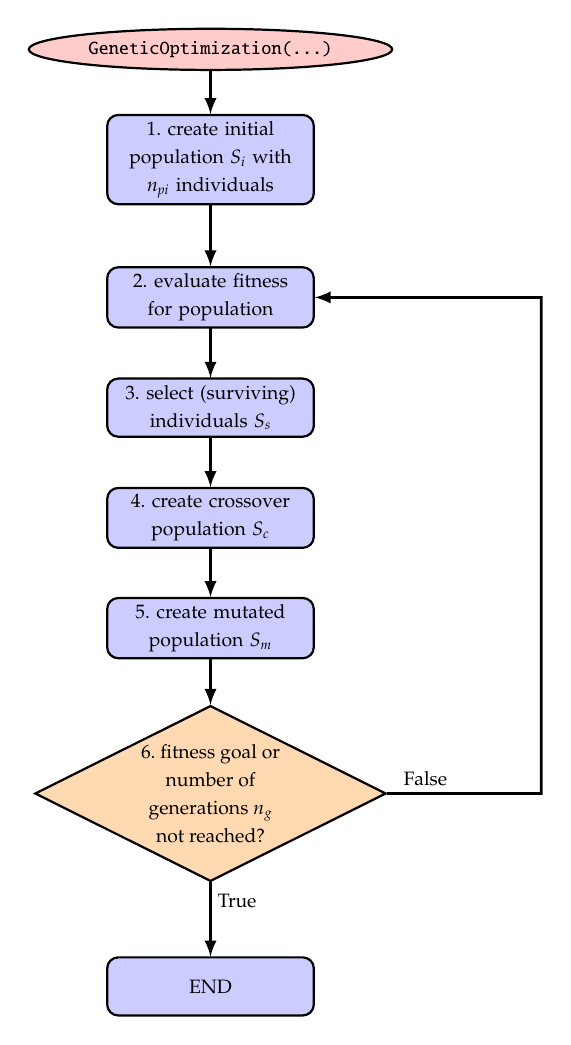
\begin{tikzpicture}[node distance = 2cm, auto, thick,scale=0.7, every node/.style={scale=0.7}]
      % Place nodes
      \node [cloud] (geneticOptimization) {\texttt{GeneticOptimization(...)}};
%      \node [wideblock, below of=init_solver_specific] (initializeSolver) {InitializeSolver()};
      \node [wideblock, below of=geneticOptimization, node distance=2cm] (initial) {1.\ create initial population $S_i$ with $n_{pi}$ individuals};
      \node [wideblock, below of=initial, node distance=2.5cm] (fitness) {2.\ evaluate fitness for population};
      \node [wideblock, below of=fitness] (surviving) {3.\ select (surviving) individuals $S_s$};
      \node [wideblock, below of=surviving] (crossover) {4.\ create crossover population $S_c$};
      \node [wideblock, below of=crossover] (mutation) {5.\ create mutated population $S_m$};
      \node [decision, below of=mutation, node distance=3cm] (decision) {6.\ fitness goal or number of generations $n_g$ not reached?};
      \node [wideblock, below of=decision, node distance=3.5cm] (end) {END};
      %
      \path [arrow] (geneticOptimization) -- (initial);
      \path [arrow] (initial) -- (fitness);
      \path [arrow] (fitness) -- (surviving);
      \path [arrow] (surviving) -- (crossover);
      \path [arrow] (crossover) -- (mutation);
      \path [arrow] (mutation) -- (decision);
      \path [arrow] (decision) -- node [near start] {False} +(6cm,0) |- (fitness);
      %(D.west) -- +(-1,0) |- node[pos=0.25] {No} (C);
      \path [arrow] (decision) -- node [near start] {True}(end);
  \end{tikzpicture}
  \caption{Basic solver flow chart genetic algorithm / optimization.}
  \label{fig_geneticOptimization}
\end{figure}
}
%
For details, see the cited literature. Here, we focus on the implementation of the function 
\texttt{GeneticOptimization(...)}, see \refSection{sec:processing:GeneticOptimization}.
The initial population (step 1) is created with \texttt{initialPopulationSize} individuals with uniformly distributed random design variables $[\xv_0, \ldots, \xv_{n_{pi}-1}]$ \footnote{$\xv_i=[x_{i0}, x_{i1}, \ldots]$ being a set of genes, with single genes $x_{i0}$, $x_{i1}$, ... } in the search space, which is given in the dictionary \texttt{parameters}. Herafter (steps 2-6), we iteratively process a population for a certain \texttt{numberOfGenerations} generations.

In step 3, the surviving individuals $S_s$ with best fitness (smallest value from evaluation of \texttt{objectiveFunction}) are selected and considered further in the optimization. If the \texttt{distanceFactor} is used, the surviving individuals must be located within a certain distance (measured relative to the range of the search space) to all other surviving individuals. This option guarantees the search within several local minima, while a conventional search often converges to one single minimum.
Crossover (step 4)  is performed using a crossover of all available parameters of two randomly selected parents when generating children from the surviving individuals. The crossover of genes is performed only for a part of the new population, defined by \texttt{crossoverAmount}.

Finally, in step 5, we apply mutation to all genes, which extends the search to the surrounding design space of the individuals created by crossover. The mutation could be performed by means of certain distribution functions in order to focus on the currently best search regions. However, in the current implementation of \texttt{GeneticOptimization(...)} we simply use a uniform random variable to distribute the genes over a certain percentage of the design space, which is reduced in every generation defined by the \texttt{rangeReductionFactor} $r_r$. This allows us to restrict further search to a smaller subregion of the design space and in general allows a reduction of search space by means of $r_r^{n_g}$. In the ideal case, using sufficiently large population sizes and being lucky with the found random values, a range reduction factor $r_r=0.7$ reduces the search space by a factor of $100$ after every 13 generations, allowing to obtain 4 digits of accuracy for design variables after 26 generations for suitable optimization problems.

It should be noted that still this optimization method is based on random values and thus may fail occasionally for any problem case. In order to get reproducible results, set \texttt{randomizerInitialization} to any integer value (simply: 0) in order to get identical results for repeated runs. Setting the latter variable guarantees that the Python (numpy) randomizer creates the same series of random values for initial population, mutation, etc.





\clearpage
}

%+++++++++++++++++++++++++++++++++++++
\mysection{Issues and bugs}
\label{sec:issueTracker}
\iftoggle{compileAll}
{
\renewcommand{\baselinestretch}{1.0} %smaller linespace for issues
%automatically generated by issueTracker
%
This section contains resolved issues per release and known bugs. Use this information to understand changes compared to previous versions. The author field is omitted if it was Johannes Gerstmayr (JG).
The extension \texttt{.dev1} is not added in the issues list (e.g., 1.2.2.dev1==1.2.2), as it only marks versions that will not be available in pypi with standard pip install, but only with the \texttt{-}\texttt{-pre} option or by specifying the exact version name, see versions on \exuUrl{https://pypi.org/project/exudyn/}{https://pypi.org/project/exudyn/}.
BUG numbers refer to the according issue numbers.




\noindent General information on current version:
\bi \small
  \item Exudyn version = 1.6.80.dev1, 
  \item last change =  2023-04-28, 
  \item Number of issues = 1540, 
  \item Number of resolved issues = 1360 (80 in current version), 
\ei

\mysubsection{Resolved issues and resolved bugs}
\par \noindent The following list contains the issues which have been {\bf RESOLVED} in the according version:
\bi \setlength\itemsep{-4pt} \scriptsize 
  \item[] {\bf Version 1.6.80}:  resolved Issue 1538: {\bf taskmanager}
(fix)
\vspace{-6pt}   \begin{itemize} \setlength\itemsep{-1pt}
    \item {description: fix problem with taskmanager shutdown due to issue 1532}
    \item   date resolved: {\bf 2023-04-27 15:35},
date raised: 2023-04-27 
  \ei
  \item[] {\bf Version 1.6.79}:  resolved Issue 1537: {\bf output.multiThreadingMode}
(fix)
\vspace{-6pt}   \begin{itemize} \setlength\itemsep{-1pt}
    \item {description: has not been set correctly in solver so far; switch output.numberOfThreadsUsed and output.multiThreadingMode}
    \item   date resolved: {\bf 2023-04-27 15:35},
date raised: 2023-04-27 
  \ei
  \item[] {\bf Version 1.6.78}:  resolved Issue 1535: {\bf writeSensors}
(extension)
\vspace{-6pt}   \begin{itemize} \setlength\itemsep{-1pt}
    \item {description: add global flag to deactivate sensor file creating/writing and sensor storing; set flag in solver functions such as ComputeLinearizedSystem, etc. to avoid erasing sensor files or sensor data}
    \item   date resolved: {\bf 2023-04-27 11:34},
date raised: 2023-04-26 
  \ei
  \item[] {\bf Version 1.6.77}:  resolved Issue 1533: {\bf FinalizeSolver}
(fix)
\vspace{-6pt}   \begin{itemize} \setlength\itemsep{-1pt}
    \item {description: call FinalizeSolver in ComputeLinearizedSystem, ComputeSystemDegreeOfFreedom, ComputeODE2Eigenvalues for consistency reason; also deactivate file writing and sensor writing and solverInformation writing}
    \item   date resolved: {\bf 2023-04-26 19:25},
date raised: 2023-04-26 
  \ei
  \item[] {\bf Version 1.6.76}:  resolved Issue 1532: {\bf CSolverBase.cpp}
(fix)
\vspace{-6pt}   \begin{itemize} \setlength\itemsep{-1pt}
    \item {description: close output and sensor files in destructor of CSolverBase}
    \item   date resolved: {\bf 2023-04-26 19:24},
date raised: 2023-04-26 
  \ei
  \item[] {\bf Version 1.6.75}:  resolved Issue 1534: {\bf EXUlie}
(change)
\vspace{-6pt}   \begin{itemize} \setlength\itemsep{-1pt}
    \item {description: improve TExpSE3 and TExpSE3Inv regarding small values according to PhD thesis of Stefan Hante}
    \item {\bf notes: improves numerical behavior and convergence of GeometricallyExactBeam}
    \item   date resolved: {\bf 2023-04-26 18:33},
date raised: 2023-04-26 
  \ei
  \item[] {\bf Version 1.6.74}:  resolved Issue 1531: {\bf OpenVR}
(fix)
\vspace{-6pt}   \begin{itemize} \setlength\itemsep{-1pt}
    \item {description: change order of eye transformation and projection in OpenVRinterface GetCurrentViewProjectionMatrix to be consistent with master thesis}
    \item   date resolved: {\bf 2023-04-26 16:49},
date raised: 2023-04-26 
  \ei
  \item[] {\bf Version 1.6.73}:  resolved Issue 1530: {\bf ComputeSystemDegreeOfFreedom}
(extension)
\vspace{-6pt}   \begin{itemize} \setlength\itemsep{-1pt}
    \item {description: add exudyn.solver function to numerically compute DOF of constrained mechanisms}
    \item   date resolved: {\bf 2023-04-26 11:16},
date raised: 2023-04-26 
  \ei
  \item[] {\bf Version 1.6.72}:  resolved Issue 1528: {\bf structures and settings}
(docu)
\vspace{-6pt}   \begin{itemize} \setlength\itemsep{-1pt}
    \item {description: function arguments in RST / html are inappropriately noted; fix; replace true/false with True/False}
    \item   date resolved: {\bf 2023-04-26 09:16},
date raised: 2023-04-26 
  \ei
  \item[] {\bf Version 1.6.71}:  resolved Issue 1527: {\bf GeneralContact}
(extension)
\vspace{-6pt}   \begin{itemize} \setlength\itemsep{-1pt}
    \item {description: add function UpdateContacts, which computes current bounding boxes and active contacts, to be used in access functions to GeneralContact if isActive=False (otherwise this is anyway done in contact computations of every computation step)}
    \item   date resolved: {\bf 2023-04-23 20:15},
date raised: 2023-04-23 
  \ei
  \item[] {\bf Version 1.6.70}:  resolved Issue 0935: {\bf GeneralContact}
(extension)
\vspace{-6pt}   \begin{itemize} \setlength\itemsep{-1pt}
    \item {description: add interface function to get contact pairs}
    \item {\bf notes: function GetActiveContacts added to GeneralContact, which returns all active global contact indices for selected contact type}
    \item   date resolved: {\bf 2023-04-23 20:13},
date raised: 2022-02-10 
  \ei
  \item[] {\bf Version 1.6.69}:  resolved Issue 1516: {\bf solver failed function}
(extension)
\vspace{-6pt}   \begin{itemize} \setlength\itemsep{-1pt}
    \item {description: add function to check if solver failed, using stored solver structure as input; return True/False and string (optionally error code) describing failure}
    \item {\bf notes: added function SolverSuccess() to exudyn.solver; returns success and error string as created by solver internal function GetErrorString(...)}
    \item   date resolved: {\bf 2023-04-23 18:43},
date raised: 2023-04-19 
  \ei
  \item[] {\bf Version 1.6.68}:  resolved Issue 1526: {\bf solver GetErrorString}
(extension)
\vspace{-6pt}   \begin{itemize} \setlength\itemsep{-1pt}
    \item {description: MainSolverStatic, MainSolverExplicit, MainSolverImplicit now get function GetErrorString to obtain error string set if SolveSteps or SolveSystem failed (returned false)}
    \item   date resolved: {\bf 2023-04-23 11:46},
date raised: 2023-04-23 
  \ei
  \item[] {\bf Version 1.6.67}:  resolved Issue 1525: {\bf output.finishedSuccessfully}
(extension)
\vspace{-6pt}   \begin{itemize} \setlength\itemsep{-1pt}
    \item {description: flag is now set both in SolveSteps(...) as well in SolveSystem(...) to indicate if solver has been successful or failed; practical flag for lateron determination of solver errors}
    \item   date resolved: {\bf 2023-04-23 11:46},
date raised: 2023-04-23 
  \ei
  \item[] {\bf Version 1.6.66}:  resolved Issue 1524: {\bf netgen STL file}
(examples)
\vspace{-6pt}   \begin{itemize} \setlength\itemsep{-1pt}
    \item {description: add example with netgen and STL files with meshing}
    \item   date resolved: {\bf 2023-04-21 17:51},
date raised: 2023-04-21 
  \ei
  \item[] {\bf Version 1.6.65}:  resolved Issue 1521: {\bf ObjectFFRFreducedOrderInterface}
(extension)
\vspace{-6pt}   \begin{itemize} \setlength\itemsep{-1pt}
    \item {description: add LoadFromFile/SaveToFile similar to FEMinterface}
    \item {\bf notes: this function should be used to store CMS data if FEM is too large to load/store; CMS data still stores all node positions, triangle list (for visualization) and modeBasis for computation tasks; may be still large e.g. for many nodes and large number of modes}
    \item   date resolved: {\bf 2023-04-20 21:06},
date raised: 2023-04-20 
  \ei
  \item[] {\bf Version 1.6.64}:  resolved Issue 1519: {\bf FEMinterface}
(change)
\vspace{-6pt}   \begin{itemize} \setlength\itemsep{-1pt}
    \item {description: add version to LoadFromFile/SaveToFile function; store file version as first field to load/store in order to be able to load older data as well; use forceVersion=0 to load files in old format}
    \item {\bf notes: warning is printed if old file is loaded}
    \item   date resolved: {\bf 2023-04-20 20:59},
date raised: 2023-04-19 
  \ei
  \item[] {\bf Version 1.6.63}:  resolved Issue 1523: {\bf StrNodeType2NodeType}
(extension)
\vspace{-6pt}   \begin{itemize} \setlength\itemsep{-1pt}
    \item {description: add function to rigidBodyUtilities in order to make str to type conversion}
    \item   date resolved: {\bf 2023-04-20 18:34},
date raised: 2023-04-20 
  \ei
  \item[] {\bf Version 1.6.62}:  resolved Issue 1522: {\bf ObjectFFRFreducedOrderInterface}
(change)
\vspace{-6pt}   \begin{itemize} \setlength\itemsep{-1pt}
    \item {description: remove femInterface from internal variables, as it is only used for postProcessingModes; store postProcessingModes instead}
    \item   date resolved: {\bf 2023-04-20 16:34},
date raised: 2023-04-20 
  \ei
  \item[] {\bf Version 1.6.61}:  resolved Issue 1520: {\bf ImportFromAbaqusInputFile}
(change)
\vspace{-6pt}   \begin{itemize} \setlength\itemsep{-1pt}
    \item {description: use VolumeToSurfaceElements for creating of surface elements; add option to automatically create surface triangles}
    \item {\bf notes: by default, only surface triangles are created!}
    \item   date resolved: {\bf 2023-04-20 15:44},
date raised: 2023-04-20 
  \ei
  \item[] {\bf Version 1.6.60}:  resolved Issue 1518: {\bf ObjectFFRFreducedOrderInterface}
(fix)
\vspace{-6pt}   \begin{itemize} \setlength\itemsep{-1pt}
    \item {description: roundMassMatrix and roundStiffnessMatrix are not used}
    \item {\bf notes: added as arguments in RoundMatrix}
    \item   date resolved: {\bf 2023-04-19 19:08},
date raised: 2023-04-19 
  \ei
  \item[] {\bf Version 1.6.59}:  resolved Issue 1517: {\bf ImportFromAbaqusInputFile}
(extension)
\vspace{-6pt}   \begin{itemize} \setlength\itemsep{-1pt}
    \item {description: extended for Tet4 and Tet10 as well as C3D20R elements and added function ConvertTetToTrigs(...)}
    \item   date resolved: {\bf 2023-04-19 18:14},
date raised: 2023-04-19 
  \ei
  \item[] {\bf Version 1.6.58}:  resolved Issue 1515: {\bf unused header files}
(cleanup)
\vspace{-6pt}   \begin{itemize} \setlength\itemsep{-1pt}
    \item {description: remove unused header files for C, Main and Visu: JointPrismatic.h, JointRevolute.h}
    \item   date resolved: {\bf 2023-04-16 13:03},
date raised: 2023-04-16 
  \ei
  \item[] {\bf Version 1.6.57}:  resolved Issue 1269: {\bf LaserSensor}
(extension)
\vspace{-6pt}   \begin{itemize} \setlength\itemsep{-1pt}
    \item {description: add advanced distance sensors replicating laser scanner (with axis, revolution speed and initial direction)}
    \item {\bf notes: added function AddLidar(...) into exudyn.robotics.utilities; see laserScannerTest.py}
    \item   date resolved: {\bf 2023-04-15 15:33},
date raised: 2022-09-21 
  \ei
  \item[] {\bf Version 1.6.56}:  resolved Issue 1270: {\bf DistanceSensor}
(extension)
\vspace{-6pt}   \begin{itemize} \setlength\itemsep{-1pt}
    \item {description: add advanced distance sensor with possibility to use a set of beams and averaging or multiple output}
    \item {\bf notes: added DistanceSensorSetupGeometry in exudyn.utilities to set up contact geometry easily; see laserScannerTest.py}
    \item   date resolved: {\bf 2023-04-15 15:32},
date raised: 2022-09-21 
  \ei
  \item[] {\bf Version 1.6.55}: {\bf \color{warningRed}  resolved BUG 1514}: {\bf GetInterpolatedSignalValue}
\vspace{-6pt}   \begin{itemize} \setlength\itemsep{-1pt}
    \item {description: check for simple test, seems not to work}
    \item {\bf notes: changed order of args: dataArrayIndex and timeArrayIndex}
    \item   date resolved: {\bf 2023-04-15 14:34},
date raised: 2023-04-14 
  \ei
  \item[] {\bf Version 1.6.54}:  resolved Issue 1513: {\bf RevoluteJoint, PrismaticJoint}
(fix)
\vspace{-6pt}   \begin{itemize} \setlength\itemsep{-1pt}
    \item {description: both ObjectJointPrismaticX and ObjectJointRevoluteZ have wrong internal typename JointRevolute; change to correct names; when analyzing such objects, they will return wrong typenames}
    \item   date resolved: {\bf 2023-04-14 14:36},
date raised: 2023-04-14 
  \ei
  \item[] {\bf Version 1.6.53}:  resolved Issue 1511: {\bf AddDistanceSensor}
(extension)
\vspace{-6pt}   \begin{itemize} \setlength\itemsep{-1pt}
    \item {description: add optional color for laser beam}
    \item   date resolved: {\bf 2023-04-13 17:45},
date raised: 2023-04-13 
  \ei
  \item[] {\bf Version 1.6.52}: {\bf \color{warningRed}  resolved BUG 1510}: {\bf AddDistanceSensor}
\vspace{-6pt}   \begin{itemize} \setlength\itemsep{-1pt}
    \item {description: checks performed with invalid marker number}
    \item   date resolved: {\bf 2023-04-13 10:28},
date raised: 2023-04-13 
  \ei
  \item[] {\bf Version 1.6.51}:  resolved Issue 1141: {\bf object factory}
(extension)
\vspace{-6pt}   \begin{itemize} \setlength\itemsep{-1pt}
    \item {description: consider hash tables for object factory; check current performance?}
    \item {\bf notes: no changes; string comparison has no effect on performance as compared to new and pybind11 overheads for call to  AddObject, etc.}
    \item   date resolved: {\bf 2023-04-10 21:48},
date raised: 2022-06-12 
  \ei
  \item[] {\bf Version 1.6.50}:  resolved Issue 1506: {\bf ODE2Size}
(fix)
\vspace{-6pt}   \begin{itemize} \setlength\itemsep{-1pt}
    \item {description: and other functions have additional ConfigurationType: remove}
    \item {\bf notes: kept the argument ConfigurationType; usually, all configuration types have same sizes but the call must be related to a speficic configuration}
    \item   date resolved: {\bf 2023-04-10 21:42},
date raised: 2023-04-08 
  \ei
  \item[] {\bf Version 1.6.49}:  resolved Issue 1509: {\bf SystemData}
(fix)
\vspace{-6pt}   \begin{itemize} \setlength\itemsep{-1pt}
    \item {description: prevent from creation of a pure SystemData in exudyn; check constructor used in SC.AddSystem and SystemData()}
    \item   date resolved: {\bf 2023-04-10 21:37},
date raised: 2023-04-10 
  \ei
  \item[] {\bf Version 1.6.48}:  resolved Issue 1508: {\bf MainSystem}
(fix)
\vspace{-6pt}   \begin{itemize} \setlength\itemsep{-1pt}
    \item {description: prevent from creation of a pure MainSystem in exudyn; check constructor used in SC.AddSystem and MainSystem()}
    \item   date resolved: {\bf 2023-04-10 21:37},
date raised: 2023-04-10 
  \ei
  \item[] {\bf Version 1.6.47}:  resolved Issue 1507: {\bf SystemContainer}
(docu)
\vspace{-6pt}   \begin{itemize} \setlength\itemsep{-1pt}
    \item {description: add description for SystemContainer itself; sying that it behaves like a variable in Python}
    \item   date resolved: {\bf 2023-04-10 21:36},
date raised: 2023-04-10 
  \ei
  \item[] {\bf Version 1.6.46}:  resolved Issue 1503: {\bf item description}
(docu)
\vspace{-6pt}   \begin{itemize} \setlength\itemsep{-1pt}
    \item {description: add general description to RST / sphinx}
    \item   date resolved: {\bf 2023-04-08 19:04},
date raised: 2023-04-08 
  \ei
  \item[] {\bf Version 1.6.45}:  resolved Issue 1496: {\bf AddMainObjectPyClass}
(check)
\vspace{-6pt}   \begin{itemize} \setlength\itemsep{-1pt}
    \item {description: C++: for adding objects, nodes, etc. currently py::object and py::dict is copied: check performance increase, if it is passed by reference}
    \item {\bf notes: tests show small performance improvements (<10 percent) for creation of items}
    \item   date resolved: {\bf 2023-04-08 17:36},
date raised: 2023-04-07 
  \ei
  \item[] {\bf Version 1.6.44}:  resolved Issue 1498: {\bf MarkerNodeRotationCoordinate}
(check)
\vspace{-6pt}   \begin{itemize} \setlength\itemsep{-1pt}
    \item {description: check if Orientation type is correct, see docu}
    \item {\bf notes: removed Marker::Orientation from MarkerNodeRotationCoordinate as it is not provided}
    \item   date resolved: {\bf 2023-04-08 17:30},
date raised: 2023-04-08 
  \ei
  \item[] {\bf Version 1.6.43}: {\bf \color{warningRed}  resolved BUG 1497}: {\bf PyBeamSection}
\vspace{-6pt}   \begin{itemize} \setlength\itemsep{-1pt}
    \item {description: C++: segmentation fault in linux, caused by conversion from numpy array into std::array; use SetConstMatrixTemplateSafely for writing matrix or list}
    \item   date resolved: {\bf 2023-04-07 19:05},
date raised: 2023-04-07 
  \ei
  \item[] {\bf Version 1.6.42}: {\bf \color{warningRed}  resolved BUG 1495}: {\bf BeamSection}
\vspace{-6pt}   \begin{itemize} \setlength\itemsep{-1pt}
    \item {description: PyBeamSection does not call parent constructor (BeamSection); leads to seg fault in linux version}
    \item   date resolved: {\bf 2023-04-07 13:32},
date raised: 2023-04-07 
  \ei
  \item[] {\bf Version 1.6.41}:  resolved Issue 1272: {\bf GeometricallyExactBeam}
(check)
\vspace{-6pt}   \begin{itemize} \setlength\itemsep{-1pt}
    \item {description: check jacobian computation as numerical differentiation works better; similar to \#1100}
    \item {\bf notes: fixed bug of GeometricallyExactBeam having wrong jacobian}
    \item   date resolved: {\bf 2023-04-06 18:28},
date raised: 2022-09-24 
  \ei
  \item[] {\bf Version 1.6.40}:  resolved Issue 1492: {\bf Python utilities}
(docu)
\vspace{-6pt}   \begin{itemize} \setlength\itemsep{-1pt}
    \item {description: fix indentation of examples}
    \item   date resolved: {\bf 2023-04-06 14:55},
date raised: 2023-04-06 
  \ei
  \item[] {\bf Version 1.6.39}:  resolved Issue 1491: {\bf ProcessParameterList}
(fix)
\vspace{-6pt}   \begin{itemize} \setlength\itemsep{-1pt}
    \item {description: remove addComputationIndex, as it is unused}
    \item   date resolved: {\bf 2023-04-06 14:35},
date raised: 2023-04-06 
  \ei
  \item[] {\bf Version 1.6.38}:  resolved Issue 1156: {\bf renderState}
(docu)
\vspace{-6pt}   \begin{itemize} \setlength\itemsep{-1pt}
    \item {description: add description of render state from C++ into theDoc}
    \item {\bf notes: added section Render State in section Graphics and Visualization (GUI)}
    \item   date resolved: {\bf 2023-04-05 14:14},
date raised: 2022-06-21 
  \ei
  \item[] {\bf Version 1.6.37}:  resolved Issue 1468: {\bf sphinx}
(docu)
\vspace{-6pt}   \begin{itemize} \setlength\itemsep{-1pt}
    \item {description: add issue and bugs section with resolved issues and open issues table; resolved issues with version}
    \item {\bf notes: already done earlier}
    \item   date resolved: {\bf 2023-04-05 14:08},
date raised: 2023-03-22 
  \ei
  \item[] {\bf Version 1.6.36}:  resolved Issue 1490: {\bf ANCFBeam}
(change)
\vspace{-6pt}   \begin{itemize} \setlength\itemsep{-1pt}
    \item {description: remove testBeamRectangularSize}
    \item   date resolved: {\bf 2023-04-05 13:59},
date raised: 2023-04-05 
  \ei
  \item[] {\bf Version 1.6.35}:  resolved Issue 1088: {\bf ANCFBeam3D}
(extension)
\vspace{-6pt}   \begin{itemize} \setlength\itemsep{-1pt}
    \item {description: add test model, compare to 2013 paper}
    \item   date resolved: {\bf 2023-04-04 20:59},
date raised: 2022-05-16 
  \ei
  \item[] {\bf Version 1.6.34}: {\bf \color{warningRed}  resolved BUG 1489}: {\bf CObjectANCFBeam}
\vspace{-6pt}   \begin{itemize} \setlength\itemsep{-1pt}
    \item {description: Computation of elastic forces uses global instead of local twist-and-curvature vector}
    \item   date resolved: {\bf 2023-04-04 20:04},
date raised: 2023-04-04 
  \ei
  \item[] {\bf Version 1.6.33}:  resolved Issue 1488: {\bf NodePoint3DSlope23}
(extension)
\vspace{-6pt}   \begin{itemize} \setlength\itemsep{-1pt}
    \item {description: add full rigid body output values to node (e.g., Rotation missing)}
    \item   date resolved: {\bf 2023-04-04 13:31},
date raised: 2023-04-04 
  \ei
  \item[] {\bf Version 1.6.32}:  resolved Issue 1487: {\bf Acceleration}
(extension)
\vspace{-6pt}   \begin{itemize} \setlength\itemsep{-1pt}
    \item {description: add GetAcceleration function to all nodes; add acceleration to all ODE2-based node output variables}
    \item   date resolved: {\bf 2023-04-04 13:27},
date raised: 2023-04-04 
  \ei
  \item[] {\bf Version 1.6.31}:  resolved Issue 1482: {\bf EnterTaskManager}
(change)
\vspace{-6pt}   \begin{itemize} \setlength\itemsep{-1pt}
    \item {description: removed call to EnterTaskManager in serial mode as it causes large overhead; also removed large array for tracer}
    \item   date resolved: {\bf 2023-03-28 18:47},
date raised: 2023-03-28 
  \ei
  \item[] {\bf Version 1.6.30}:  resolved Issue 1481: {\bf InverseKinematicsNumerical}
(change)
\vspace{-6pt}   \begin{itemize} \setlength\itemsep{-1pt}
    \item {description: changed SolveIKine to Solve and changed OutputVariable Rotation to RotationMatrix at tool}
    \item   date resolved: {\bf 2023-03-28 16:30},
date raised: 2023-03-28 
  \ei
  \item[] {\bf Version 1.6.29}:  resolved Issue 1480: {\bf LogSE3}
(extension)
\vspace{-6pt}   \begin{itemize} \setlength\itemsep{-1pt}
    \item {description: fixed according to LogSO3 and added efficient version with vectors in C++}
    \item   date resolved: {\bf 2023-03-28 15:10},
date raised: 2023-03-28 
  \ei
  \item[] {\bf Version 1.6.28}:  resolved Issue 1478: {\bf LogSO3}
(fix)
\vspace{-6pt}   \begin{itemize} \setlength\itemsep{-1pt}
    \item {description: Add new LogSO3 C++ function, also to be used in LogSE3 which fully works for 0..pi rotation range; improved accuracy for very small rotations as well as rotations close to pi, e.g. 0.99999999*pi, where the standard approach fails}
    \item   date resolved: {\bf 2023-03-28 15:09},
date raised: 2023-03-27 
  \ei
  \item[] {\bf Version 1.6.27}:  resolved Issue 1469: {\bf RotationMatrix2Rxyz}
(fix)
\vspace{-6pt}   \begin{itemize} \setlength\itemsep{-1pt}
    \item {description: extend implementation for rot[1]=pi/2}
    \item {\bf notes: resolved both in Python and C++; some simulation results may change, especially in output of Rotations in sensors}
    \item   date resolved: {\bf 2023-03-28 14:46},
date raised: 2023-03-22 
  \ei
  \item[] {\bf Version 1.6.26}:  resolved Issue 1477: {\bf LogSO3}
(fix)
\vspace{-6pt}   \begin{itemize} \setlength\itemsep{-1pt}
    \item {description: Add new LogSO3 Python function, also to be used in LogSE3 which fully works for 0..pi rotation range; improved accuracy for very small rotations as well as rotations close to pi, e.g. 0.99999999*pi, where the standard approach fails}
    \item   date resolved: {\bf 2023-03-27 20:16},
date raised: 2023-03-27 
  \ei
  \item[] {\bf Version 1.6.25}:  resolved Issue 1476: {\bf RotationMatrix2...}
(fix)
\vspace{-6pt}   \begin{itemize} \setlength\itemsep{-1pt}
    \item {description: RotationMatrix2EulerParameters, RotationMatrix2RotXYZ, RotationMatrix2RotZYZ not working both with list of lists and np.arrays}
    \item   date resolved: {\bf 2023-03-27 19:58},
date raised: 2023-03-27 
  \ei
  \item[] {\bf Version 1.6.23}:  resolved Issue 0312: {\bf Add all types to pybind}
(extension)
\vspace{-6pt}   \begin{itemize} \setlength\itemsep{-1pt}
    \item {description: add remaining types to pybind - for user elements}
    \item {\bf notes: important types already added; further types currently not planned}
    \item   date resolved: {\bf 2023-03-27 00:45},
date raised: 2020-01-10 
  \ei
  \item[] {\bf Version 1.6.22}:  resolved Issue 0848: {\bf add demos to github}
(docu)
\vspace{-6pt}   \begin{itemize} \setlength\itemsep{-1pt}
    \item {description: add demo videos to github or to youtube}
    \item {\bf notes: already resolved earlier: added videos to youtube}
    \item   date resolved: {\bf 2023-03-27 00:42},
date raised: 2021-12-26 
  \ei
  \item[] {\bf Version 1.6.21}:  resolved Issue 0843: {\bf connector jacobian springDamper}
(extension)
\vspace{-6pt}   \begin{itemize} \setlength\itemsep{-1pt}
    \item {description: add analytic jacobian for SpringDamper connector}
    \item {\bf notes: already resolved earlier}
    \item   date resolved: {\bf 2023-03-27 00:42},
date raised: 2021-12-23 
  \ei
  \item[] {\bf Version 1.6.20}:  resolved Issue 0851: {\bf ComputeObjectODE2LHS}
(extension)
\vspace{-6pt}   \begin{itemize} \setlength\itemsep{-1pt}
    \item {description: add computation functions for bodies and connectors; for connectors, markerData is computed automatically}
    \item {\bf notes: already resolved earlier with precomputed lists}
    \item   date resolved: {\bf 2023-03-27 00:40},
date raised: 2022-01-08 
  \ei
  \item[] {\bf Version 1.6.19}:  resolved Issue 1325: {\bf MergeGraphicsDataTriangleList}
(fix)
\vspace{-6pt}   \begin{itemize} \setlength\itemsep{-1pt}
    \item {description: merging of edges erroneous or problems with GraphicsDataCylinder}
    \item   date resolved: {\bf 2023-03-27 00:21},
date raised: 2022-12-19 
  \ei
  \item[] {\bf Version 1.6.18}:  resolved Issue 1472: {\bf GraphicsData}
(extension)
\vspace{-6pt}   \begin{itemize} \setlength\itemsep{-1pt}
    \item {description: add addEdges option to all GraphicsData Python functions}
    \item {\bf notes: added to sphere, cylinder, SolidOfRevolution, SolidOfExtrusion}
    \item   date resolved: {\bf 2023-03-27 00:10},
date raised: 2023-03-26 
  \ei
  \item[] {\bf Version 1.6.17}:  resolved Issue 1473: {\bf GraphicsData}
(change)
\vspace{-6pt}   \begin{itemize} \setlength\itemsep{-1pt}
    \item {description: improve edges of cylinder and sphere by adding 6 lines along cylinder, some circles for sphere}
    \item   date resolved: {\bf 2023-03-27 00:09},
date raised: 2023-03-26 
  \ei
  \item[] {\bf Version 1.6.16}:  resolved Issue 1459: {\bf mention papers}
(docu)
\vspace{-6pt}   \begin{itemize} \setlength\itemsep{-1pt}
    \item {description: add list of papers where exudyn has been used in theDoc and RTD}
    \item   date resolved: {\bf 2023-03-26 15:04},
date raised: 2023-03-10 
  \ei
  \item[] {\bf Version 1.6.15}:  resolved Issue 1471: {\bf issues tracker}
(docu)
\vspace{-6pt}   \begin{itemize} \setlength\itemsep{-1pt}
    \item {description: remove html file from docs, use RSTfiles instead / move to readthedocs}
    \item   date resolved: {\bf 2023-03-24 20:40},
date raised: 2023-03-24 
  \ei
  \item[] {\bf Version 1.6.14}:  resolved Issue 1470: {\bf GraphicsDataBasis}
(extension)
\vspace{-6pt}   \begin{itemize} \setlength\itemsep{-1pt}
    \item {description: add orientation and duplicate function with homogeneous transformation (HT) argument}
    \item {\bf notes: function called GraphicsDataFrame for Homogeneous transformation}
    \item   date resolved: {\bf 2023-03-24 10:04},
date raised: 2023-03-24 
  \ei
  \item[] {\bf Version 1.6.13}:  resolved Issue 1467: {\bf InverseKinematicsNumerical}
(fix)
\vspace{-6pt}   \begin{itemize} \setlength\itemsep{-1pt}
    \item {description: fix success}
    \item   date resolved: {\bf 2023-03-22 12:06},
date raised: 2023-03-22 (resolved by: P. Manzl)
  \ei
  \item[] {\bf Version 1.6.12}:  resolved Issue 1466: {\bf modKKDH}
(change)
\vspace{-6pt}   \begin{itemize} \setlength\itemsep{-1pt}
    \item {description: consistently renamed into modDHKK in robotics module}
    \item   date resolved: {\bf 2023-03-22 11:04},
date raised: 2023-03-22 
  \ei
  \item[] {\bf Version 1.6.11}:  resolved Issue 1465: {\bf robotics.models}
(change)
\vspace{-6pt}   \begin{itemize} \setlength\itemsep{-1pt}
    \item {description: adjust robot definitions, add dhMode to dictionary; fix LinkList2Robot}
    \item   date resolved: {\bf 2023-03-22 10:39},
date raised: 2023-03-22 
  \ei
  \item[] {\bf Version 1.6.10}:  resolved Issue 1464: {\bf artificialIntelligence}
(fix)
\vspace{-6pt}   \begin{itemize} \setlength\itemsep{-1pt}
    \item {description: adapt to stable-baselines3 > 1.5.0; Class OpenAIGymInterfaceEnv does not support stable-baselines3 > 1.5.0 because OpenAIGymInterfaceEnv is not inherited from gym.Env}
    \item   date resolved: {\bf 2023-03-20 12:54},
date raised: 2023-03-20 (resolved by: P. Manzl)
  \ei
  \item[] {\bf Version 1.6.9}:  resolved Issue 1463: {\bf mpi4py}
(extension)
\vspace{-6pt}   \begin{itemize} \setlength\itemsep{-1pt}
    \item {description: add option to use MPI (message passing interface) for ProcessParameterList}
    \item {\bf notes: tests on supercomputer successful}
    \item   date resolved: {\bf 2023-03-18 22:59},
date raised: 2023-03-18 
  \ei
  \item[] {\bf Version 1.6.8}:  resolved Issue 1462: {\bf minimum coordinates}
(docu)
\vspace{-6pt}   \begin{itemize} \setlength\itemsep{-1pt}
    \item {description: change consistently to minimal coordinates}
    \item   date resolved: {\bf 2023-03-14 17:39},
date raised: 2023-03-14 
  \ei
  \item[] {\bf Version 1.6.7}: {\bf \color{warningRed}  resolved BUG 1461}: {\bf isIntType check ParameterVariation}
\vspace{-6pt}   \begin{itemize} \setlength\itemsep{-1pt}
    \item {description: In the ParameterVariation (part of the processing module)  the integer type check failed when Variables of different types were used, now checking each variable independently}
    \item {\bf notes: added isIntType arrays}
    \item   date resolved: {\bf 2023-03-14 12:50},
date raised: 2023-03-14 (resolved by: P. Manzl)
  \ei
  \item[] {\bf Version 1.6.6}:  resolved Issue 1457: {\bf Newton}
(docu)
\vspace{-6pt}   \begin{itemize} \setlength\itemsep{-1pt}
    \item {description: fix steps and Newton iterations in description of Newton settings (thanks to Martin Arnold!)}
    \item   date resolved: {\bf 2023-03-12 23:05},
date raised: 2023-03-09 
  \ei
  \item[] {\bf Version 1.6.5}:  resolved Issue 1456: {\bf sphinx/github pages}
(docu)
\vspace{-6pt}   \begin{itemize} \setlength\itemsep{-1pt}
    \item {description: add examples and test models for better search results}
    \item   date resolved: {\bf 2023-03-12 23:05},
date raised: 2023-03-09 
  \ei
  \item[] {\bf Version 1.6.4}:  resolved Issue 1445: {\bf sphinx/github pages}
(docu)
\vspace{-6pt}   \begin{itemize} \setlength\itemsep{-1pt}
    \item {description: add solver description}
    \item   date resolved: {\bf 2023-03-12 23:05},
date raised: 2023-02-22 
  \ei
  \item[] {\bf Version 1.6.3}:  resolved Issue 1443: {\bf sphinx/github pages}
(docu)
\vspace{-6pt}   \begin{itemize} \setlength\itemsep{-1pt}
    \item {description: add theory parts as far as possible}
    \item   date resolved: {\bf 2023-03-12 23:05},
date raised: 2023-02-22 
  \ei
  \item[] {\bf Version 1.6.2}:  resolved Issue 1460: {\bf theDoc}
(docu)
\vspace{-6pt}   \begin{itemize} \setlength\itemsep{-1pt}
    \item {description: change structure: theory, notations earlier; remove duplicated MatrixContainer description}
    \item   date resolved: {\bf 2023-03-12 16:20},
date raised: 2023-03-12 
  \ei
  \item[] {\bf Version 1.6.1}:  resolved Issue 1458: {\bf artificialIntelligence nan test}
(extension)
\vspace{-6pt}   \begin{itemize} \setlength\itemsep{-1pt}
    \item {description: check for nan values in TestModel evaluation}
    \item {\bf notes: failed steps may lead to nan values when evaluating the TestModel in the artificialIntelligence module. When this is detected the flagNan is set and evaluation is stopped. Check for flagNan in the Evaluation should be implemented.}
    \item   date resolved: {\bf 2023-03-10 15:59},
date raised: 2023-03-10 (resolved by: P. Manzl)
  \ei
  \item[] {\bf Version 1.6.0}:  resolved Issue 1426: {\bf cleanup howto files}
(fix)
\vspace{-6pt}   \begin{itemize} \setlength\itemsep{-1pt}
    \item {description: check if info is still valid (NGsolve, WSL, anaconda, ...)}
    \item {\bf notes: removed outdated files}
    \item   date resolved: {\bf 2023-03-08 16:58},
date raised: 2023-02-11 
  \ei
  \item[] {\bf Version 1.5.118}:  resolved Issue 1454: {\bf julia}
(docu)
\vspace{-6pt}   \begin{itemize} \setlength\itemsep{-1pt}
    \item {description: add sub section on interoperability with julia in Overview on Exudyn / Advanced topics; add some relevant examples for usage}
    \item   date resolved: {\bf 2023-03-05 16:40},
date raised: 2023-03-05 
  \ei
  \item[] {\bf Version 1.5.117}:  resolved Issue 1453: {\bf \_\_NOGLFW option not working}
(fix)
\vspace{-6pt}   \begin{itemize} \setlength\itemsep{-1pt}
    \item {description: exclude according functions in rendererPythonInterface}
    \item {\bf notes: added NOGLFW version to automatic build and testsuite}
    \item   date resolved: {\bf 2023-02-28 15:18},
date raised: 2023-02-28 
  \ei
  \item[] {\bf Version 1.5.116}:  resolved Issue 1452: {\bf Single command}
(docu)
\vspace{-6pt}   \begin{itemize} \setlength\itemsep{-1pt}
    \item {description: add some more detailed description in theDoc after Visualization settings dialog}
    \item   date resolved: {\bf 2023-02-26 00:40},
date raised: 2023-02-26 
  \ei
  \item[] {\bf Version 1.5.115}:  resolved Issue 1451: {\bf solver interface}
(check)
\vspace{-6pt}   \begin{itemize} \setlength\itemsep{-1pt}
    \item {description: check modification of solver structures like it to be writable}
    \item {\bf notes: added now write functionality for solvers; use with care and only if you know what you do...}
    \item   date resolved: {\bf 2023-02-26 00:12},
date raised: 2023-02-25 
  \ei
  \item[] {\bf Version 1.5.114}:  resolved Issue 1447: {\bf CSensorMarker}
(extension)
\vspace{-6pt}   \begin{itemize} \setlength\itemsep{-1pt}
    \item {description: add RotationMatrix as additional outputvariable type}
    \item {\bf notes: Coordinates also added as output variable}
    \item   date resolved: {\bf 2023-02-24 15:46},
date raised: 2023-02-23 
  \ei
  \item[] {\bf Version 1.5.113}:  resolved Issue 1446: {\bf CSensorMarker}
(fix)
\vspace{-6pt}   \begin{itemize} \setlength\itemsep{-1pt}
    \item {description: does not check types; Make GetOutputVariableTypes as in objects; orientation only for selected markers; check types in Assemble prechecks}
    \item   date resolved: {\bf 2023-02-24 15:46},
date raised: 2023-02-23 
  \ei
  \item[] {\bf Version 1.5.112}: {\bf \color{warningRed}  resolved BUG 1449}: {\bf DOPRI5}
\vspace{-6pt}   \begin{itemize} \setlength\itemsep{-1pt}
    \item {description: small bug introduced in previous update: currentStepSize not updated any more}
    \item   date resolved: {\bf 2023-02-24 15:45},
date raised: 2023-02-24 
  \ei
  \item[] {\bf Version 1.5.111}:  resolved Issue 1448: {\bf GenericJoint}
(extension)
\vspace{-6pt}   \begin{itemize} \setlength\itemsep{-1pt}
    \item {description: add experimental flag alternativeConstraints to switch to different constraint equations, e.g. for 3 constrained rotations; this resolves unphysical 180 degree flips especially in static cases; flag may be removed in future}
    \item {\bf notes: thanks for P. Manzl for raising this problem}
    \item   date resolved: {\bf 2023-02-24 13:52},
date raised: 2023-02-24 
  \ei
  \item[] {\bf Version 1.5.110}:  resolved Issue 1444: {\bf sphinx/github pages}
(docu)
\vspace{-6pt}   \begin{itemize} \setlength\itemsep{-1pt}
    \item {description: fix equation references and figures}
    \item   date resolved: {\bf 2023-02-24 13:50},
date raised: 2023-02-22 
  \ei
  \item[] {\bf Version 1.5.109}:  resolved Issue 1442: {\bf add readthedocs.io}
(docu)
\vspace{-6pt}   \begin{itemize} \setlength\itemsep{-1pt}
    \item {description: link github project to readthedocs.io site}
    \item   date resolved: {\bf 2023-02-22 23:59},
date raised: 2023-02-22 
  \ei
  \item[] {\bf Version 1.5.108}:  resolved Issue 1441: {\bf sphinx/github pages}
(docu)
\vspace{-6pt}   \begin{itemize} \setlength\itemsep{-1pt}
    \item {description: add more parts on items (equations)}
    \item   date resolved: {\bf 2023-02-22 23:57},
date raised: 2023-02-22 
  \ei
  \item[] {\bf Version 1.5.107}:  resolved Issue 1440: {\bf ParameterVariation}
(change)
\vspace{-6pt}   \begin{itemize} \setlength\itemsep{-1pt}
    \item {description: integer should be kept as integers, if they are provided as a list and if variation is only on integers}
    \item {\bf notes: integers are kept if either tuple(start, end, numberOfValues) with start/end and numberOfValues are all integer or list contains only integers}
    \item   date resolved: {\bf 2023-02-22 13:46},
date raised: 2023-02-22 (resolved by: S. Holzinger)
  \ei
  \item[] {\bf Version 1.5.106}:  resolved Issue 1439: {\bf numpy dependency}
(extension)
\vspace{-6pt}   \begin{itemize} \setlength\itemsep{-1pt}
    \item {description: add install\_requires to setup.py to force numpy to be installed; exudynCPP always requires now numpy}
    \item   date resolved: {\bf 2023-02-21 18:11},
date raised: 2023-02-21 
  \ei
  \item[] {\bf Version 1.5.105}:  resolved Issue 1438: {\bf sphinx / github pages}
(docu)
\vspace{-6pt}   \begin{itemize} \setlength\itemsep{-1pt}
    \item {description: add input/output tables for items in RST files}
    \item   date resolved: {\bf 2023-02-21 10:14},
date raised: 2023-02-19 
  \ei
  \item[] {\bf Version 1.5.104}:  resolved Issue 1437: {\bf sphinx / github pages}
(docu)
\vspace{-6pt}   \begin{itemize} \setlength\itemsep{-1pt}
    \item {description: add items to RST files/Sphinx to show up on github pages}
    \item   date resolved: {\bf 2023-02-19 21:39},
date raised: 2023-02-19 
  \ei
  \item[] {\bf Version 1.5.103}:  resolved Issue 1436: {\bf sphinx / github pages}
(docu)
\vspace{-6pt}   \begin{itemize} \setlength\itemsep{-1pt}
    \item {description: add settings and structures; fix latex parts; fix links}
    \item   date resolved: {\bf 2023-02-18 00:56},
date raised: 2023-02-18 
  \ei
  \item[] {\bf Version 1.5.102}: {\bf \color{warningRed}  resolved BUG 1433}: {\bf Lie group integration}
\vspace{-6pt}   \begin{itemize} \setlength\itemsep{-1pt}
    \item {description: system with > 1 node raises LinkedDataVectorBases exception}
    \item   date resolved: {\bf 2023-02-16 16:00},
date raised: 2023-02-16 
  \ei
  \item[] {\bf Version 1.5.101}:  resolved Issue 1432: {\bf artificialIntelligence module}
(fix)
\vspace{-6pt}   \begin{itemize} \setlength\itemsep{-1pt}
    \item {description: fix np.float64 not beeing detected as a scalar (float) for initializationValues of RL environment and possible waiting without activated renderer}
    \item   date resolved: {\bf 2023-02-16 15:58},
date raised: 2023-02-16 (resolved by: P. Manzl)
  \ei
  \item[] {\bf Version 1.5.100}:  resolved Issue 1431: {\bf make github pages}
(extension)
\vspace{-6pt}   \begin{itemize} \setlength\itemsep{-1pt}
    \item {description: install workflow for github pages to host pages for exudyn}
    \item {\bf notes: due to automatic conversion, there are many small errors (typos) remaining; for safety, check theDoc.pdf in any case}
    \item   date resolved: {\bf 2023-02-16 00:01},
date raised: 2023-02-16 
  \ei
  \item[] {\bf Version 1.5.99}:  resolved Issue 1430: {\bf create rst docu files}
(extension)
\vspace{-6pt}   \begin{itemize} \setlength\itemsep{-1pt}
    \item {description: Create rst (markup language) files for C++ command interface and Python utilities}
    \item   date resolved: {\bf 2023-02-16 00:00},
date raised: 2023-02-15 
  \ei
  \item[] {\bf Version 1.5.98}:  resolved Issue 1429: {\bf revise docu creation}
(fix)
\vspace{-6pt}   \begin{itemize} \setlength\itemsep{-1pt}
    \item {description: revise several helper functions for docu creation to homogenize latex and rst output}
    \item   date resolved: {\bf 2023-02-16 00:00},
date raised: 2023-02-15 
  \ei
  \item[] {\bf Version 1.5.97}:  resolved Issue 1428: {\bf ParameterVariation}
(change)
\vspace{-6pt}   \begin{itemize} \setlength\itemsep{-1pt}
    \item {description: add conversion of parameters which are numpy.float64 to float which simplifies checking agains type(float); computationIndex becomes int}
    \item   date resolved: {\bf 2023-02-13 17:18},
date raised: 2023-02-13 
  \ei
  \item[] {\bf Version 1.5.96}:  resolved Issue 1427: {\bf IsReal(x) and IsInteger(x)}
(extension)
\vspace{-6pt}   \begin{itemize} \setlength\itemsep{-1pt}
    \item {description: add checks which allow to check versus any float / numpy.float resp. int / numpy.int values; added to advancedUtilities}
    \item   date resolved: {\bf 2023-02-13 17:17},
date raised: 2023-02-13 
  \ei
  \item[] {\bf Version 1.5.95}:  resolved Issue 1425: {\bf sphinx}
(extension)
\vspace{-6pt}   \begin{itemize} \setlength\itemsep{-1pt}
    \item {description: add github pages at https://jgerstmayr.github.io/EXUDYN created with sphinx}
    \item   date resolved: {\bf 2023-02-11 16:41},
date raised: 2023-02-11 
  \ei
  \item[] {\bf Version 1.5.94}:  resolved Issue 1423: {\bf numerical Jacobians}
(change)
\vspace{-6pt}   \begin{itemize} \setlength\itemsep{-1pt}
    \item {description: add variadic template to realize numerical differentiation for objects in a consistent way}
    \item   date resolved: {\bf 2023-02-08 12:17},
date raised: 2023-02-08 
  \ei
  \item[] {\bf Version 1.5.93}:  resolved Issue 1404: {\bf Lie group method}
(fix)
\vspace{-6pt}   \begin{itemize} \setlength\itemsep{-1pt}
    \item {description: add consistent numerical derivatives for Lie group nodes, needing the composition rule for incremental changes}
    \item   date resolved: {\bf 2023-02-08 12:17},
date raised: 2023-01-18 
  \ei
  \item[] {\bf Version 1.5.92}:  resolved Issue 1422: {\bf numerical Jacobians}
(change)
\vspace{-6pt}   \begin{itemize} \setlength\itemsep{-1pt}
    \item {description: add variadic template to realize numerical differentiation in a consistent way}
    \item   date resolved: {\bf 2023-02-08 00:16},
date raised: 2023-02-07 
  \ei
  \item[] {\bf Version 1.5.91}:  resolved Issue 1421: {\bf LIE\_GROUP\_IMPLICIT\_SOLVER}
(change)
\vspace{-6pt}   \begin{itemize} \setlength\itemsep{-1pt}
    \item {description: remove preprocessor flag, as it is always set}
    \item   date resolved: {\bf 2023-02-07 12:07},
date raised: 2023-02-07 
  \ei
  \item[] {\bf Version 1.5.90}:  resolved Issue 1420: {\bf setup.py}
(extension)
\vspace{-6pt}   \begin{itemize} \setlength\itemsep{-1pt}
    \item {description: reduce output of all compiler options with --quiet mode}
    \item   date resolved: {\bf 2023-02-02 18:27},
date raised: 2023-02-02 
  \ei
  \item[] {\bf Version 1.5.89}:  resolved Issue 1419: {\bf window size}
(extension)
\vspace{-6pt}   \begin{itemize} \setlength\itemsep{-1pt}
    \item {description: window size currently limited to screen size and larger windows not accepted; override size limitations by using glfwSetWindowSize}
    \item {\bf notes: added flag window.limitWindowToScreenSize ; by default this is deactivated; added flag window.limitWindowToScreenSize ; by default this is deactivated; added flag window.limitWindowToScreenSize ; by default this is deactivated; added flag window.limitWindowToScreenSize ; by default this is deactivated; added flag window.limitWindowToScreenSize ; by default this is deactivated; added flag window.limitWindowToScreenSize ; by default this is deactivated}
    \item   date resolved: {\bf 2023-02-02 10:31},
date raised: 2023-02-02 
  \ei
  \item[] {\bf Version 1.5.88}:  resolved Issue 1418: {\bf OpenVR}
(change)
\vspace{-6pt}   \begin{itemize} \setlength\itemsep{-1pt}
    \item {description: adapt projection for OpenVR compatibility; exchange multiplication of pose and eye to fulfill classic OpenGL needs}
    \item   date resolved: {\bf 2023-02-01 10:30},
date raised: 2023-02-01 
  \ei
  \item[] {\bf Version 1.5.87}:  resolved Issue 1417: {\bf ConnectorSpringDamperExt}
(fix)
\vspace{-6pt}   \begin{itemize} \setlength\itemsep{-1pt}
    \item {description: remove unintended output during Assemble()}
    \item   date resolved: {\bf 2023-01-25 20:09},
date raised: 2023-01-25 
  \ei
  \item[] {\bf Version 1.5.86}:  resolved Issue 1405: {\bf AddDistanceSensor}
(extension)
\vspace{-6pt}   \begin{itemize} \setlength\itemsep{-1pt}
    \item {description: add rotation of Marker to ObjectGround in SensorUserFunction}
    \item {\bf notes: added option to draw displaced laser beam; rotation added, if rigid marker used}
    \item   date resolved: {\bf 2023-01-23 10:05},
date raised: 2023-01-19 
  \ei
  \item[] {\bf Version 1.5.85}:  resolved Issue 1416: {\bf AddDistanceSensor}
(fix)
\vspace{-6pt}   \begin{itemize} \setlength\itemsep{-1pt}
    \item {description: UFsensorDistance misses the rotation part in visualization of laser beam with ground object}
    \item   date resolved: {\bf 2023-01-23 09:39},
date raised: 2023-01-23 
  \ei
  \item[] {\bf Version 1.5.84}:  resolved Issue 1413: {\bf CoordinateSpringDamperExt}
(change)
\vspace{-6pt}   \begin{itemize} \setlength\itemsep{-1pt}
    \item {description: change friction parameter dimensions to forces (because there is no normal force) and change parameter names}
    \item   date resolved: {\bf 2023-01-22 23:43},
date raised: 2023-01-21 
  \ei
  \item[] {\bf Version 1.5.83}:  resolved Issue 1412: {\bf CoordinateSpringDamperExt}
(extension)
\vspace{-6pt}   \begin{itemize} \setlength\itemsep{-1pt}
    \item {description: finalize implementation for bristle friction model}
    \item   date resolved: {\bf 2023-01-22 23:43},
date raised: 2023-01-21 
  \ei
  \item[] {\bf Version 1.5.82}:  resolved Issue 1411: {\bf CoordinateSpringDamperExt}
(extension)
\vspace{-6pt}   \begin{itemize} \setlength\itemsep{-1pt}
    \item {description: finalize implementation for limit stops}
    \item   date resolved: {\bf 2023-01-22 23:43},
date raised: 2023-01-21 
  \ei
  \item[] {\bf Version 1.5.81}:  resolved Issue 1410: {\bf examples}
(change)
\vspace{-6pt}   \begin{itemize} \setlength\itemsep{-1pt}
    \item {description: adapt Examples/massSpringFrictionInteractive.py and Examples/lugreFrictionTest.py to new CoordinateSpringDamperExt}
    \item   date resolved: {\bf 2023-01-21 22:04},
date raised: 2023-01-21 
  \ei
  \item[] {\bf Version 1.5.80}:  resolved Issue 1136: {\bf ConnectorsExt}
(extension)
\vspace{-6pt}   \begin{itemize} \setlength\itemsep{-1pt}
    \item {description: add extended Ext versions of connectors: CoordinateSpringDamperExt, TorsionalSpringDamperExt, LinearSpringDamperExt, which allow for friction, coordinate limitation (with other SD-values) and possibly future extensions}
    \item   date resolved: {\bf 2023-01-21 21:29},
date raised: 2022-06-10 
  \ei
  \item[] {\bf Version 1.5.79}:  resolved Issue 1407: {\bf pause}
(extension)
\vspace{-6pt}   \begin{itemize} \setlength\itemsep{-1pt}
    \item {description: add option for pause by pressing space bar}
    \item   date resolved: {\bf 2023-01-21 21:28},
date raised: 2023-01-21 
  \ei
  \item[] {\bf Version 1.5.78}:  resolved Issue 1409: {\bf CoordinateSpringDamper}
(change)
\vspace{-6pt}   \begin{itemize} \setlength\itemsep{-1pt}
    \item {description: remove dryFriction and dryFrictionProportionalZone; this functionality will be made available in CoordinateSpringDamperExt}
    \item {\bf notes: see CoordinateSpringDamper in theDoc.pdf how to convert old models using friction parameters to new ones; note user function interfaces have been changed!}
    \item   date resolved: {\bf 2023-01-21 17:53},
date raised: 2023-01-21 
  \ei
  \item[] {\bf Version 1.5.77}:  resolved Issue 1408: {\bf WaitForUserToContinue}
(extension)
\vspace{-6pt}   \begin{itemize} \setlength\itemsep{-1pt}
    \item {description: add argument printMessage, which can be set false to avoid text output in console; default behavior preserved}
    \item   date resolved: {\bf 2023-01-21 13:51},
date raised: 2023-01-21 
  \ei
  \item[] {\bf Version 1.5.76}:  resolved Issue 1406: {\bf git tags}
(extension)
\vspace{-6pt}   \begin{itemize} \setlength\itemsep{-1pt}
    \item {description: add git tags for every new version automatically}
    \item {\bf notes: now versions can be found easier in github and they match the version numbers in pypi with pip installer}
    \item   date resolved: {\bf 2023-01-19 18:47},
date raised: 2023-01-19 
  \ei
  \item[] {\bf Version 1.5.75}:  resolved Issue 1314: {\bf Pybind11}
(check)
\vspace{-6pt}   \begin{itemize} \setlength\itemsep{-1pt}
    \item {description: test compilation with higher version of pybind11 (currently pybind11=2.6.0 in setup.py}
    \item {\bf notes: already done earlier; works well and allows compilation with Python3.11; added some switches in setup.py as not all Pybind11 versions work everywhere}
    \item   date resolved: {\bf 2023-01-19 01:04},
date raised: 2022-12-14 
  \ei
  \item[] {\bf Version 1.5.74}:  resolved Issue 1365: {\bf OpenVR}
(example)
\vspace{-6pt}   \begin{itemize} \setlength\itemsep{-1pt}
    \item {description: add Python example with openVR}
    \item   date resolved: {\bf 2023-01-19 01:02},
date raised: 2023-01-03 
  \ei
  \item[] {\bf Version 1.5.73}:  resolved Issue 1326: {\bf OpenVR}
(change)
\vspace{-6pt}   \begin{itemize} \setlength\itemsep{-1pt}
    \item {description: add OpenVR license and mention in getting started}
    \item   date resolved: {\bf 2023-01-19 01:02},
date raised: 2022-12-20 
  \ei
  \item[] {\bf Version 1.5.72}:  resolved Issue 1402: {\bf openVR}
(extension)
\vspace{-6pt}   \begin{itemize} \setlength\itemsep{-1pt}
    \item {description: add flag to set compilation with openVR in setup.py; copy .dll in Windows case}
    \item   date resolved: {\bf 2023-01-18 22:57},
date raised: 2023-01-17 
  \ei
  \item[] {\bf Version 1.5.71}:  resolved Issue 1364: {\bf OpenVR}
(extension)
\vspace{-6pt}   \begin{itemize} \setlength\itemsep{-1pt}
    \item {description: test simple use case}
    \item {\bf notes: basic functionality added; enable compilation with openVR by setting '-D\_\_EXUDYN\_USE\_OPENVR' in cpp compiler flags of setup.py}
    \item   date resolved: {\bf 2023-01-17 09:32},
date raised: 2023-01-03 (resolved by: EXTENSION)
  \ei
  \item[] {\bf Version 1.5.70}:  resolved Issue 1401: {\bf lockModelView}
(extension)
\vspace{-6pt}   \begin{itemize} \setlength\itemsep{-1pt}
    \item {description: add flag which allows to fully lock rotation, zoom, etc.; in this case, only initial values in openGL settings are accepted for setup of view, but mouse or key input is ignored}
    \item   date resolved: {\bf 2023-01-17 09:20},
date raised: 2023-01-17 
  \ei
  \item[] {\bf Version 1.5.69}:  resolved Issue 1363: {\bf test OpenVR with basic OpenGL}
(check)
\vspace{-6pt}   \begin{itemize} \setlength\itemsep{-1pt}
    \item {description: check if current openGL is sufficient with textures}
    \item   date resolved: {\bf 2023-01-16 23:11},
date raised: 2023-01-03 
  \ei
  \item[] {\bf Version 1.5.68}:  resolved Issue 1400: {\bf renderState}
(change)
\vspace{-6pt}   \begin{itemize} \setlength\itemsep{-1pt}
    \item {description: vectors and matrices are returned in numpy format; this allows simpler computation, but does not anymore allow to treat output as list (+ operator!)}
    \item   date resolved: {\bf 2023-01-16 21:11},
date raised: 2023-01-16 
  \ei
  \item[] {\bf Version 1.5.67}:  resolved Issue 1399: {\bf renderState}
(change)
\vspace{-6pt}   \begin{itemize} \setlength\itemsep{-1pt}
    \item {description: initialization now done consistently for SC.AttachToRenderEngine() and exudyn.StartRenderer(); behavior should be as before}
    \item   date resolved: {\bf 2023-01-16 21:10},
date raised: 2023-01-16 
  \ei
  \item[] {\bf Version 1.5.66}:  resolved Issue 1398: {\bf renderState}
(extension)
\vspace{-6pt}   \begin{itemize} \setlength\itemsep{-1pt}
    \item {description: add projectionMatrix containing the current projection usd (usually identity matrix)}
    \item   date resolved: {\bf 2023-01-16 20:09},
date raised: 2023-01-16 
  \ei
  \item[] {\bf Version 1.5.65}:  resolved Issue 1397: {\bf showFaceEdges, showMeshEdges}
(fix)
\vspace{-6pt}   \begin{itemize} \setlength\itemsep{-1pt}
    \item {description: wrong switching causing to show edges only if also some faces are activated}
    \item   date resolved: {\bf 2023-01-12 22:32},
date raised: 2023-01-12 
  \ei
  \item[] {\bf Version 1.5.64}:  resolved Issue 1387: {\bf Get...Output}
(extension)
\vspace{-6pt}   \begin{itemize} \setlength\itemsep{-1pt}
    \item {description: add way to work for Reference configuration}
    \item {\bf notes: nodes, bodies and markers allow reference configuration; sensors also allow it for GetSensorValues}
    \item   date resolved: {\bf 2023-01-12 22:14},
date raised: 2023-01-12 
  \ei
  \item[] {\bf Version 1.5.63}:  resolved Issue 1389: {\bf configuration checks}
(extension)
\vspace{-6pt}   \begin{itemize} \setlength\itemsep{-1pt}
    \item {description: check all systemData C++ interface functions regarding illegal configuration}
    \item   date resolved: {\bf 2023-01-12 22:03},
date raised: 2023-01-12 
  \ei
  \item[] {\bf Version 1.5.62}:  resolved Issue 1388: {\bf configuration checks}
(extension)
\vspace{-6pt}   \begin{itemize} \setlength\itemsep{-1pt}
    \item {description: IsConfigurationInitialCurrentReferenceVisualization and IsConfigurationInitialCurrentVisualization shall be extended for StartOfStep; add hint that a calling function may have used an illegal configuration or None}
    \item   date resolved: {\bf 2023-01-12 22:03},
date raised: 2023-01-12 
  \ei
  \item[] {\bf Version 1.5.61}:  resolved Issue 1396: {\bf Demo}
(extnesion)
\vspace{-6pt}   \begin{itemize} \setlength\itemsep{-1pt}
    \item {description: add a two demos included into the python module; put into exudyn.demos; add hint for larger examples; Demo1() = without graphics, just creating output file; Demo2() is rigid3Dexample with SolutionViewer}
    \item   date resolved: {\bf 2023-01-12 18:51},
date raised: 2023-01-12 
  \ei
  \item[] {\bf Version 1.5.60}:  resolved Issue 1385: {\bf help}
(extension)
\vspace{-6pt}   \begin{itemize} \setlength\itemsep{-1pt}
    \item {description: add exudyn.help() function for short notes}
    \item   date resolved: {\bf 2023-01-12 18:04},
date raised: 2023-01-12 
  \ei
  \item[] {\bf Version 1.5.59}: {\bf \color{warningRed}  resolved BUG 1390}: {\bf ComputeLinearizedSystem}
\vspace{-6pt}   \begin{itemize} \setlength\itemsep{-1pt}
    \item {description: not working because of wrong interface to ComputeJacobianODE2RHS}
    \item   date resolved: {\bf 2023-01-12 17:53},
date raised: 2023-01-12 
  \ei
  \item[] {\bf Version 1.5.58}:  resolved Issue 1394: {\bf eigenvalues test}
(testing)
\vspace{-6pt}   \begin{itemize} \setlength\itemsep{-1pt}
    \item {description: refine test model for ComputeODE2Eigenvalues}
    \item   date resolved: {\bf 2023-01-12 17:44},
date raised: 2023-01-12 
  \ei
  \item[] {\bf Version 1.5.57}:  resolved Issue 1393: {\bf ComputeJacobianAE}
(change)
\vspace{-6pt}   \begin{itemize} \setlength\itemsep{-1pt}
    \item {description: change default values to fit to conventional tangential stiffness matrix computation}
    \item   date resolved: {\bf 2023-01-12 17:00},
date raised: 2023-01-12 
  \ei
  \item[] {\bf Version 1.5.56}:  resolved Issue 1392: {\bf ComputeJacobianODE1RHS}
(change)
\vspace{-6pt}   \begin{itemize} \setlength\itemsep{-1pt}
    \item {description: change default values to fit to conventional tangential stiffness matrix computation}
    \item   date resolved: {\bf 2023-01-12 17:00},
date raised: 2023-01-12 
  \ei
  \item[] {\bf Version 1.5.55}:  resolved Issue 1391: {\bf ComputeJacobianODE2RHS}
(change)
\vspace{-6pt}   \begin{itemize} \setlength\itemsep{-1pt}
    \item {description: change default values to fit to conventional tangential stiffness matrix computation}
    \item   date resolved: {\bf 2023-01-12 17:00},
date raised: 2023-01-12 
  \ei
  \item[] {\bf Version 1.5.54}: {\bf \color{warningRed}  resolved BUG 1386}: {\bf GetMarkerOutput}
\vspace{-6pt}   \begin{itemize} \setlength\itemsep{-1pt}
    \item {description: crashes if used with any configuration before Assemble(); add check that it may be only called after Assemble()}
    \item {\bf notes: add check and raise error}
    \item   date resolved: {\bf 2023-01-12 14:15},
date raised: 2023-01-12 
  \ei
  \item[] {\bf Version 1.5.53}:  resolved Issue 1384: {\bf visualizationSettings}
(extension)
\vspace{-6pt}   \begin{itemize} \setlength\itemsep{-1pt}
    \item {description: add textOffsetFactor in general options to adjust text offset if not drawn always in front}
    \item {\bf notes: also adjusted some text appearance settings}
    \item   date resolved: {\bf 2023-01-11 20:42},
date raised: 2023-01-11 
  \ei
  \item[] {\bf Version 1.5.52}:  resolved Issue 1383: {\bf visualizationSettings}
(docu)
\vspace{-6pt}   \begin{itemize} \setlength\itemsep{-1pt}
    \item {description: update docu of Visualization settings dialog in introduction}
    \item   date resolved: {\bf 2023-01-11 17:41},
date raised: 2023-01-11 
  \ei
  \item[] {\bf Version 1.5.51}:  resolved Issue 1382: {\bf visualizationSettings}
(change)
\vspace{-6pt}   \begin{itemize} \setlength\itemsep{-1pt}
    \item {description: increase initial size of visualizations dialog for larger screens; see  \refSection{sec:overview:basics:visualizationsettings} how to change to a smaller window size}
    \item   date resolved: {\bf 2023-01-11 16:57},
date raised: 2023-01-11 
  \ei
  \item[] {\bf Version 1.5.50}:  resolved Issue 1381: {\bf visualizationSettings}
(change)
\vspace{-6pt}   \begin{itemize} \setlength\itemsep{-1pt}
    \item {description: change order of items to have easier access to each tree node}
    \item {\bf notes: dialogs.openTreeView=True can be used to switch to original behavior}
    \item   date resolved: {\bf 2023-01-11 16:34},
date raised: 2023-01-11 
  \ei
  \item[] {\bf Version 1.5.49}:  resolved Issue 1379: {\bf item text color}
(change)
\vspace{-6pt}   \begin{itemize} \setlength\itemsep{-1pt}
    \item {description: draw colors in item texts (node numbers, etc.) different from item color to improve visibility}
    \item   date resolved: {\bf 2023-01-11 16:28},
date raised: 2023-01-11 
  \ei
  \item[] {\bf Version 1.5.48}:  resolved Issue 1308: {\bf OpenGL texts}
(extension)
\vspace{-6pt}   \begin{itemize} \setlength\itemsep{-1pt}
    \item {description: add sub function for drawing text bitmaps; use different order of drawing for transparent and non-transparent triangles to get improved text drawing}
    \item {\bf notes: now having possibility to draw item texts in front or transparent}
    \item   date resolved: {\bf 2023-01-11 16:28},
date raised: 2022-12-08 
  \ei
  \item[] {\bf Version 1.5.47}:  resolved Issue 1380: {\bf loads}
(change)
\vspace{-6pt}   \begin{itemize} \setlength\itemsep{-1pt}
    \item {description: draw load numbers at end of load vectors}
    \item {\bf notes: made Force consistent with Torque and LoadMassProportional}
    \item   date resolved: {\bf 2023-01-11 14:43},
date raised: 2023-01-11 
  \ei
  \item[] {\bf Version 1.5.46}:  resolved Issue 1378: {\bf font drawing}
(extension)
\vspace{-6pt}   \begin{itemize} \setlength\itemsep{-1pt}
    \item {description: add visualizationSettings.general for textDrawInFront and textHasBackGround for having a (currently) white background color}
    \item   date resolved: {\bf 2023-01-11 09:46},
date raised: 2023-01-11 
  \ei
  \item[] {\bf Version 1.5.45}:  resolved Issue 1377: {\bf openvr}
(change)
\vspace{-6pt}   \begin{itemize} \setlength\itemsep{-1pt}
    \item {description: not compatible right now with Exudyn under Windows while linux seems to work}
    \item   date resolved: {\bf 2023-01-09 21:11},
date raised: 2023-01-09 
  \ei
  \item[] {\bf Version 1.5.44}:  resolved Issue 1370: {\bf advancedUtilities}
(extension)
\vspace{-6pt}   \begin{itemize} \setlength\itemsep{-1pt}
    \item {description: add advanced utilities depnding on numpy and math; functions not suitable for exudyn.basicUtilities or exudyn.utilities}
    \item   date resolved: {\bf 2023-01-07 01:57},
date raised: 2023-01-06 
  \ei
  \item[] {\bf Version 1.5.43}:  resolved Issue 1375: {\bf initial accelerations}
(extension)
\vspace{-6pt}   \begin{itemize} \setlength\itemsep{-1pt}
    \item {description: add flag to decide whether initial accelerations are erased at beginning of simulation; the background is that they should not be erased, if they are prolonged for subsequent simulation; check if this changes behavior, as ODE2\_tt coordinates are anyway resetted at Assemble()}
    \item   date resolved: {\bf 2023-01-07 01:56},
date raised: 2023-01-06 
  \ei
  \item[] {\bf Version 1.5.42}:  resolved Issue 1376: {\bf advancedUtilities}
(change)
\vspace{-6pt}   \begin{itemize} \setlength\itemsep{-1pt}
    \item {description: move functions exudyn.utilities from to exudyn.advancedUtilities; still included in exudyn.utilities}
    \item   date resolved: {\bf 2023-01-06 22:54},
date raised: 2023-01-06 
  \ei
  \item[] {\bf Version 1.5.41}: {\bf \color{warningRed}  resolved BUG 1374}: {\bf InteractiveDialog}
\vspace{-6pt}   \begin{itemize} \setlength\itemsep{-1pt}
    \item {description: accelerations are not reused from last period; need to copy current accelerations into initial accelerations}
    \item   date resolved: {\bf 2023-01-06 21:21},
date raised: 2023-01-06 
  \ei
  \item[] {\bf Version 1.5.40}:  resolved Issue 1373: {\bf GraphicsData}
(change)
\vspace{-6pt}   \begin{itemize} \setlength\itemsep{-1pt}
    \item {description: add option to add edges in GraphicsData...Cube... functions; switch some order of options }
    \item   date resolved: {\bf 2023-01-06 19:25},
date raised: 2023-01-06 
  \ei
  \item[] {\bf Version 1.5.39}:  resolved Issue 1372: {\bf utilities}
(fix)
\vspace{-6pt}   \begin{itemize} \setlength\itemsep{-1pt}
    \item {description: ComputeSkewMatrix: remove duplicate (with less functionality) from utilities and put into rigidBodyUtilities; correct import in FEM}
    \item   date resolved: {\bf 2023-01-06 19:19},
date raised: 2023-01-06 
  \ei
  \item[] {\bf Version 1.5.38}:  resolved Issue 1371: {\bf exudyn.utilities}
(change)
\vspace{-6pt}   \begin{itemize} \setlength\itemsep{-1pt}
    \item {description: remove functions CheckInputVector and CheckInputIndexArray as they are unused and replaced with improved functions in advancedUtilities}
    \item   date resolved: {\bf 2023-01-06 17:46},
date raised: 2023-01-06 
  \ei
  \item[] {\bf Version 1.5.37}:  resolved Issue 1369: {\bf add sub-module machines}
(extension)
\vspace{-6pt}   \begin{itemize} \setlength\itemsep{-1pt}
    \item {description: will include mechanical engineering and machine element relevant topics, such as bearings, gears, mechanisms, etc.}
    \item   date resolved: {\bf 2023-01-06 11:47},
date raised: 2023-01-06 
  \ei
  \item[] {\bf Version 1.5.36}:  resolved Issue 1368: {\bf GraphicsDataCylinder}
(extension)
\vspace{-6pt}   \begin{itemize} \setlength\itemsep{-1pt}
    \item {description: new option to only add edges without faces}
    \item   date resolved: {\bf 2023-01-05 23:03},
date raised: 2023-01-05 
  \ei
  \item[] {\bf Version 1.5.35}:  resolved Issue 1367: {\bf GraphicsDataSolidExtrusion}
(extension)
\vspace{-6pt}   \begin{itemize} \setlength\itemsep{-1pt}
    \item {description: add edges and normals for smoothening}
    \item   date resolved: {\bf 2023-01-05 23:03},
date raised: 2023-01-05 
  \ei
  \item[] {\bf Version 1.5.34}:  resolved Issue 1366: {\bf GraphicsData}
(extension)
\vspace{-6pt}   \begin{itemize} \setlength\itemsep{-1pt}
    \item {description: add functionality for GraphicsDataSolidExtrusion to include circles: CirclePointsAndSegments() and to manipulate point lists defining geometries: SegmentsFromPoints()}
    \item   date resolved: {\bf 2023-01-05 18:15},
date raised: 2023-01-05 
  \ei
  \item[] {\bf Version 1.5.33}:  resolved Issue 1362: {\bf add OpenVR interface}
(extension)
\vspace{-6pt}   \begin{itemize} \setlength\itemsep{-1pt}
    \item {description: add interface, but by default not compiled}
    \item   date resolved: {\bf 2023-01-03 23:00},
date raised: 2023-01-03 
  \ei
  \item[] {\bf Version 1.5.32}:  resolved Issue 1361: {\bf Python 3.11}
(extension)
\vspace{-6pt}   \begin{itemize} \setlength\itemsep{-1pt}
    \item {description: create first development wheels for Python 3.11; Windows+Linux}
    \item {\bf notes: problems to get conda with Python3.11 running, especially on ubuntu}
    \item   date resolved: {\bf 2023-01-03 18:48},
date raised: 2023-01-03 
  \ei
  \item[] {\bf Version 1.5.31}:  resolved Issue 1360: {\bf Python 3.11}
(extension)
\vspace{-6pt}   \begin{itemize} \setlength\itemsep{-1pt}
    \item {description: adjust setup.py to support Python 3.11; requires Pybind11 2.10}
    \item   date resolved: {\bf 2023-01-03 14:37},
date raised: 2023-01-03 
  \ei
  \item[] {\bf Version 1.5.30}:  resolved Issue 1335: {\bf RollingDiscPenalty}
(extension)
\vspace{-6pt}   \begin{itemize} \setlength\itemsep{-1pt}
    \item {description: add test example for ground moving (rotating table}
    \item   date resolved: {\bf 2023-01-02 19:07},
date raised: 2022-12-25 
  \ei
  \item[] {\bf Version 1.5.29}:  resolved Issue 1359: {\bf ObjectGround}
(extension)
\vspace{-6pt}   \begin{itemize} \setlength\itemsep{-1pt}
    \item {description: extend for referenceRotation to allow rotation of ground objects (especially for visualization and contact)}
    \item   date resolved: {\bf 2023-01-02 11:49},
date raised: 2023-01-02 
  \ei
  \item[] {\bf Version 1.5.28}:  resolved Issue 0839: {\bf multithreaded jacobian}
(extension)
\vspace{-6pt}   \begin{itemize} \setlength\itemsep{-1pt}
    \item {description: add functionality for multithreaded jacobian and mass matrix}
    \item {\bf notes: mass matrix resolved; other is redundant with \#1203}
    \item   date resolved: {\bf 2023-01-02 01:04},
date raised: 2021-12-19 
  \ei
  \item[] {\bf Version 1.5.27}:  resolved Issue 0828: {\bf MT integration2}
(extension)
\vspace{-6pt}   \begin{itemize} \setlength\itemsep{-1pt}
    \item {description: add multithreading to mass matrix and jacobian; add multithreaded adding of vector with special templated functions to allow special (templated) solver functions}
    \item {\bf notes: redundant with \#839}
    \item   date resolved: {\bf 2023-01-02 01:02},
date raised: 2021-12-09 
  \ei
  \item[] {\bf Version 1.5.26}:  resolved Issue 0791: {\bf test Eigen SimplicialLDLT}
(extension)
\vspace{-6pt}   \begin{itemize} \setlength\itemsep{-1pt}
    \item {description: use systemMatricesArePD to enable LDLT solver}
    \item {\bf notes: tested earlier; does not work in most cases}
    \item   date resolved: {\bf 2023-01-02 01:01},
date raised: 2021-11-02 
  \ei
  \item[] {\bf Version 1.5.25}:  resolved Issue 0437: {\bf solvercontainer+ systemcontainer}
(change)
\vspace{-6pt}   \begin{itemize} \setlength\itemsep{-1pt}
    \item {description: remove SolverContainer and SystemContainer from systemStructuresDefinition and work manually}
    \item {\bf notes: already done much earlier}
    \item   date resolved: {\bf 2023-01-02 00:59},
date raised: 2020-07-21 
  \ei
  \item[] {\bf Version 1.5.24}:  resolved Issue 0315: {\bf Add user object}
(extension)
\vspace{-6pt}   \begin{itemize} \setlength\itemsep{-1pt}
    \item {description: add user object}
    \item {\bf notes: done with GenericODE2 and CoordinateVectorConstraint}
    \item   date resolved: {\bf 2023-01-02 00:57},
date raised: 2020-01-10 
  \ei
  \item[] {\bf Version 1.5.23}:  resolved Issue 0261: {\bf MarkerDataJacobians}
(extension)
\vspace{-6pt}   \begin{itemize} \setlength\itemsep{-1pt}
    \item {description: Add access functions for jacobians and other marker data: SetPositionJacobian, GetPositionJacobian, etc.; add jacobian types = markertypes, which check if wrong jacobian is accessed}
    \item {\bf notes: not suitable anymore}
    \item   date resolved: {\bf 2023-01-02 00:56},
date raised: 2019-09-11 
  \ei
  \item[] {\bf Version 1.5.22}:  resolved Issue 1331: {\bf exudyn cpp}
(extension)
\vspace{-6pt}   \begin{itemize} \setlength\itemsep{-1pt}
    \item {description: add \_\_repr\_\_ and help which writes some information on workflow (github, theDoc, Examples, ...)}
    \item {\bf notes: not possible}
    \item   date resolved: {\bf 2023-01-02 00:51},
date raised: 2022-12-21 
  \ei
  \item[] {\bf Version 1.5.21}:  resolved Issue 1323: {\bf AVX2}
(extension)
\vspace{-6pt}   \begin{itemize} \setlength\itemsep{-1pt}
    \item {description: update documentation for improved functionality with AVX2 code}
    \item {\bf notes: already done when resolving \#1330}
    \item   date resolved: {\bf 2023-01-02 00:50},
date raised: 2022-12-17 
  \ei
  \item[] {\bf Version 1.5.20}:  resolved Issue 1355: {\bf visualizationSettings}
(check)
\vspace{-6pt}   \begin{itemize} \setlength\itemsep{-1pt}
    \item {description: check possibility for update loop to continue simulation}
    \item {\bf notes: not feasible now, as it requires to modify time integration loop}
    \item   date resolved: {\bf 2023-01-02 00:48},
date raised: 2022-12-31 
  \ei
  \item[] {\bf Version 1.5.19}:  resolved Issue 1353: {\bf visualizationSettings}
(extension)
\vspace{-6pt}   \begin{itemize} \setlength\itemsep{-1pt}
    \item {description: add KEY Q shortcut to close dialog}
    \item   date resolved: {\bf 2023-01-02 00:48},
date raised: 2022-12-31 
  \ei
  \item[] {\bf Version 1.5.18}:  resolved Issue 1358: {\bf DictionariesGetSet}
(change)
\vspace{-6pt}   \begin{itemize} \setlength\itemsep{-1pt}
    \item {description: add new types VectorFloat and MatrixFloat in order to distinguish from double values}
    \item {\bf notes: also fixed matrix conversion in visualizationSettings}
    \item   date resolved: {\bf 2023-01-02 00:47},
date raised: 2023-01-02 
  \ei
  \item[] {\bf Version 1.5.17}:  resolved Issue 1357: {\bf visualizationSettings}
(extension)
\vspace{-6pt}   \begin{itemize} \setlength\itemsep{-1pt}
    \item {description: add single click edit event}
    \item   date resolved: {\bf 2023-01-01 23:27},
date raised: 2023-01-01 
  \ei
  \item[] {\bf Version 1.5.16}:  resolved Issue 1354: {\bf visualizationSettings}
(extension)
\vspace{-6pt}   \begin{itemize} \setlength\itemsep{-1pt}
    \item {description: double click on bool variables changes state}
    \item   date resolved: {\bf 2023-01-01 23:22},
date raised: 2022-12-31 
  \ei
  \item[] {\bf Version 1.5.15}:  resolved Issue 1352: {\bf tkinter dialogs}
(fix)
\vspace{-6pt}   \begin{itemize} \setlength\itemsep{-1pt}
    \item {description: add option for transparency to dialogs}
    \item {\bf notes: visualizationSettings.dialogs.transparency}
    \item   date resolved: {\bf 2022-12-31 11:01},
date raised: 2022-12-31 
  \ei
  \item[] {\bf Version 1.5.14}:  resolved Issue 1351: {\bf tkinter MacOS}
(fix)
\vspace{-6pt}   \begin{itemize} \setlength\itemsep{-1pt}
    \item {description: adjust font size and row size in ttk right mouse dialog}
    \item {\bf notes: visualizationSettings.dialogs.fontScalingMacOS}
    \item   date resolved: {\bf 2022-12-31 11:00},
date raised: 2022-12-31 
  \ei
  \item[] {\bf Version 1.5.13}:  resolved Issue 1350: {\bf tkinter MacOS}
(fix)
\vspace{-6pt}   \begin{itemize} \setlength\itemsep{-1pt}
    \item {description: adjust font size and row size in ttk visualizationSettings dialog}
    \item {\bf notes: visualizationSettings.dialogs.fontScalingMacOS}
    \item   date resolved: {\bf 2022-12-31 11:00},
date raised: 2022-12-31 
  \ei
  \item[] {\bf Version 1.5.12}: {\bf \color{warningRed}  resolved BUG 0752}: {\bf tkinter MacOS}
\vspace{-6pt}   \begin{itemize} \setlength\itemsep{-1pt}
    \item {description: tkinter fails when loaded inside interactive.py; early call to Tk() inside an example works and seems to help; check options to correctly load tkinter in MacOS (Rosetta 2, on M1)}
    \item {\bf notes: problem fixed with single threaded renderer, doing illegal operations in glfw callbacks}
    \item   date resolved: {\bf 2022-12-31 01:01},
date raised: 2021-09-20 
  \ei
  \item[] {\bf Version 1.5.11}:  resolved Issue 1349: {\bf RequireVersion}
(fix)
\vspace{-6pt}   \begin{itemize} \setlength\itemsep{-1pt}
    \item {description: some bugs including exu.GetVersionString and not raising exception}
    \item   date resolved: {\bf 2022-12-30 15:03},
date raised: 2022-12-30 
  \ei
  \item[] {\bf Version 1.5.10}:  resolved Issue 1343: {\bf tkinter in exudyn}
(docu)
\vspace{-6pt}   \begin{itemize} \setlength\itemsep{-1pt}
    \item {description: add comment in FAQ on potential problems with tkinter; add option to let exudyn know if tkinter is already running}
    \item   date resolved: {\bf 2022-12-28 23:39},
date raised: 2022-12-27 
  \ei
  \item[] {\bf Version 1.5.9}:  resolved Issue 1347: {\bf visualizationSettings}
(extension)
\vspace{-6pt}   \begin{itemize} \setlength\itemsep{-1pt}
    \item {description: add flag visualizationSettings.dialog.multiThreadedDialogs to turn on/off immediate apply of visualizationSettings changes; extend exudyn.GUI and rendererPythonInterface.h accordingly}
    \item {\bf notes: NOTE that this flag should be turned off in case of crashes during/after dialogs; could make problems on special platforms such as MacOS}
    \item   date resolved: {\bf 2022-12-28 23:05},
date raised: 2022-12-28 
  \ei
  \item[] {\bf Version 1.5.8}:  resolved Issue 1348: {\bf EditDictionaryWithTypeInfo}
(change)
\vspace{-6pt}   \begin{itemize} \setlength\itemsep{-1pt}
    \item {description: change interface to pass directly visualizationSettings, allowing to update data}
    \item   date resolved: {\bf 2022-12-28 21:50},
date raised: 2022-12-28 
  \ei
  \item[] {\bf Version 1.5.7}:  resolved Issue 1346: {\bf visualizationSettings}
(check)
\vspace{-6pt}   \begin{itemize} \setlength\itemsep{-1pt}
    \item {description: check if visualiuation settings dialog can be installed such that updating of data immediately affects renderer window}
    \item   date resolved: {\bf 2022-12-28 16:53},
date raised: 2022-12-28 
  \ei
  \item[] {\bf Version 1.5.6}:  resolved Issue 1339: {\bf tkinter MacOS}
(fix)
\vspace{-6pt}   \begin{itemize} \setlength\itemsep{-1pt}
    \item {description: add tkinter.Tk() into exudyn.sys["tkinterRoot"] before call to StartRenderer(); check for tkinterRoot in exudyn.sys on startup of interactive dialog; resolves crash on MacOS for SolutionViewer}
    \item   date resolved: {\bf 2022-12-27 23:50},
date raised: 2022-12-26 
  \ei
  \item[] {\bf Version 1.5.5}:  resolved Issue 1345: {\bf interface default args}
(fix)
\vspace{-6pt}   \begin{itemize} \setlength\itemsep{-1pt}
    \item {description: change true/false to True/False in theDoc for PYthon command interface}
    \item   date resolved: {\bf 2022-12-27 23:24},
date raised: 2022-12-27 
  \ei
  \item[] {\bf Version 1.5.4}:  resolved Issue 1344: {\bf exudyn}
(extension)
\vspace{-6pt}   \begin{itemize} \setlength\itemsep{-1pt}
    \item {description: add function IsRendererRunning(), to avoid Warnings when renderer is restarted}
    \item   date resolved: {\bf 2022-12-27 23:23},
date raised: 2022-12-27 
  \ei
  \item[] {\bf Version 1.5.3}:  resolved Issue 1338: {\bf MacOS}
(fix)
\vspace{-6pt}   \begin{itemize} \setlength\itemsep{-1pt}
    \item {description: DoRendererIdleTasks() crashes if no Renderer is active; add check in python call to avoid crash}
    \item {\bf notes: crash resolved on Windows; MacOS test still open}
    \item   date resolved: {\bf 2022-12-27 17:36},
date raised: 2022-12-26 
  \ei
  \item[] {\bf Version 1.5.2}:  resolved Issue 1340: {\bf MacOS multithreading}
(change)
\vspace{-6pt}   \begin{itemize} \setlength\itemsep{-1pt}
    \item {description: activate simplified multithreading by switching to TinyThreading in case of MacOS}
    \item   date resolved: {\bf 2022-12-27 17:19},
date raised: 2022-12-26 
  \ei
  \item[] {\bf Version 1.5.1}:  resolved Issue 1342: {\bf MacOS M1}
(extension)
\vspace{-6pt}   \begin{itemize} \setlength\itemsep{-1pt}
    \item {description: add string ARM to Platform string, e.g., used in solution and sensor files}
    \item   date resolved: {\bf 2022-12-27 17:03},
date raised: 2022-12-27 
  \ei
  \item[] {\bf Version 1.5.0}:  resolved Issue 1336: {\bf test suite}
(fix)
\vspace{-6pt}   \begin{itemize} \setlength\itemsep{-1pt}
    \item {description: resolve linux problem with RigidBodySpringDamper.py MiniExample}
    \item {\bf notes: problem in testsuite due to AVX differences, causing all non-AVX cases to fail (also linux); fixed with special case in reference solutions}
    \item   date resolved: {\bf 2022-12-25 20:10},
date raised: 2022-12-25 
  \ei
  \item[] {\bf Version 1.4.65}:  resolved Issue 1264: {\bf RollingDiscPenalty}
(extension)
\vspace{-6pt}   \begin{itemize} \setlength\itemsep{-1pt}
    \item {description: correct torque on ground, which currently has no effect, but will be used for moving ground}
    \item {\bf notes: resolved earlier}
    \item   date resolved: {\bf 2022-12-25 12:15},
date raised: 2022-09-17 
  \ei
  \item[] {\bf Version 1.4.64}:  resolved Issue 1298: {\bf ReevingSystemLinear}
(testing)
\vspace{-6pt}   \begin{itemize} \setlength\itemsep{-1pt}
    \item {description: add test model to test suite}
    \item   date resolved: {\bf 2022-12-25 12:11},
date raised: 2022-12-01 
  \ei
  \item[] {\bf Version 1.4.63}:  resolved Issue 1333: {\bf gcc linux}
(change)
\vspace{-6pt}   \begin{itemize} \setlength\itemsep{-1pt}
    \item {description: adjust -march compilation options for improved performance on linux; try -march=skylake for AVX2 optimization}
    \item {\bf notes: did not work: either gives compilation errors or segmentation faults}
    \item   date resolved: {\bf 2022-12-25 00:45},
date raised: 2022-12-24 
  \ei
  \item[] {\bf Version 1.4.62}:  resolved Issue 1334: {\bf NOGLFW}
(change)
\vspace{-6pt}   \begin{itemize} \setlength\itemsep{-1pt}
    \item {description: remove SystemContainer constructor warning for AttachToRenderEngine in case of NOGLFW}
    \item {\bf notes: also done for DetachFromRenderEngine}
    \item   date resolved: {\bf 2022-12-25 00:06},
date raised: 2022-12-25 
  \ei
  \item[] {\bf Version 1.4.61}:  resolved Issue 1332: {\bf MacOS}
(fix)
\vspace{-6pt}   \begin{itemize} \setlength\itemsep{-1pt}
    \item {description: compilation does not finish due to -framework Cocoa, etc. errors}
    \item {\bf notes: changed -framework library lists by separating commands into two separate strings; compilation now runs through for Python 3.8-3.10 on MacOS with M1 and 3.7.-3.10 on \_x86 emulation}
    \item   date resolved: {\bf 2022-12-24 22:20},
date raised: 2022-12-24 
  \ei
  \item[] {\bf Version 1.4.60}:  resolved Issue 1330: {\bf AVX2}
(fix)
\vspace{-6pt}   \begin{itemize} \setlength\itemsep{-1pt}
    \item {description: fix check for AVX and AVX2 on module import}
    \item   date resolved: {\bf 2022-12-21 19:33},
date raised: 2022-12-21 
  \ei
  \item[] {\bf Version 1.4.59}:  resolved Issue 1329: {\bf SolutionViewer}
(example)
\vspace{-6pt}   \begin{itemize} \setlength\itemsep{-1pt}
    \item {description: add example for SolutionViewer with multiple static simulations performed, writing results into single file; see Examples/solutionViewerMultipleSimulations.py}
    \item   date resolved: {\bf 2022-12-21 18:05},
date raised: 2022-12-21 
  \ei
  \item[] {\bf Version 1.4.58}:  resolved Issue 1328: {\bf simulationSettings.solutionSettings}
(extension)
\vspace{-6pt}   \begin{itemize} \setlength\itemsep{-1pt}
    \item {description: add option writeInitialValues in order to turn on/off writing of initial values for coordinatesSolution and sensors; by default turned on as was done so far}
    \item   date resolved: {\bf 2022-12-21 14:07},
date raised: 2022-12-21 
  \ei
  \item[] {\bf Version 1.4.57}:  resolved Issue 1037: {\bf sensor files}
(extension)
\vspace{-6pt}   \begin{itemize} \setlength\itemsep{-1pt}
    \item {description: add file footer information same as in coordinatesSolutionFile including CPUtimeElapsed with 3 digits}
    \item {\bf notes: turned on by default, but should be switched off if it causes compatibility problems for your postprocessing tool}
    \item   date resolved: {\bf 2022-12-21 12:09},
date raised: 2022-04-07 
  \ei
  \item[] {\bf Version 1.4.56}:  resolved Issue 1327: {\bf sensorsWriteFileHeader}
(fix)
\vspace{-6pt}   \begin{itemize} \setlength\itemsep{-1pt}
    \item {description: not working}
    \item {\bf notes: added option into solver, now turning on/off as desired; added option into solver, now turning on/off as desired; added option into solver, now turning on/off as desired}
    \item   date resolved: {\bf 2022-12-21 12:06},
date raised: 2022-12-21 
  \ei
  \item[] {\bf Version 1.4.55}:  resolved Issue 1317: {\bf DistanceSensor}
(example)
\vspace{-6pt}   \begin{itemize} \setlength\itemsep{-1pt}
    \item {description: Add example with distance sensor}
    \item   date resolved: {\bf 2022-12-20 13:49},
date raised: 2022-12-16 
  \ei
  \item[] {\bf Version 1.4.54}:  resolved Issue 1318: {\bf DistanceSensor}
(extension)
\vspace{-6pt}   \begin{itemize} \setlength\itemsep{-1pt}
    \item {description: Add measurement for GeneralContact trigsRigidBody}
    \item   date resolved: {\bf 2022-12-19 21:49},
date raised: 2022-12-16 
  \ei
  \item[] {\bf Version 1.4.53}:  resolved Issue 1316: {\bf DistanceSensor}
(extension)
\vspace{-6pt}   \begin{itemize} \setlength\itemsep{-1pt}
    \item {description: add utilities function to create DistanceSensor based on general contact}
    \item {\bf notes: added AddDistanceSensor to exudyn utilities.py}
    \item   date resolved: {\bf 2022-12-19 01:09},
date raised: 2022-12-16 
  \ei
  \item[] {\bf Version 1.4.52}:  resolved Issue 1324: {\bf DistanceSensor}
(extension)
\vspace{-6pt}   \begin{itemize} \setlength\itemsep{-1pt}
    \item {description: utilities function AddDistanceSensor extended for measureVelocity to measure velocity similar as in a laser Doppler vibrometer (LDV)}
    \item   date resolved: {\bf 2022-12-18 20:59},
date raised: 2022-12-18 
  \ei
  \item[] {\bf Version 1.4.51}:  resolved Issue 1320: {\bf GeneralContact}
(extension)
\vspace{-6pt}   \begin{itemize} \setlength\itemsep{-1pt}
    \item {description: add binary contact types to pybind interface; add conversion of binary types to type indices}
    \item {\bf notes: only TypeIndex added which is sufficient for DistanceSensor}
    \item   date resolved: {\bf 2022-12-17 00:32},
date raised: 2022-12-16 
  \ei
  \item[] {\bf Version 1.4.50}:  resolved Issue 1319: {\bf DistanceSensor}
(extension)
\vspace{-6pt}   \begin{itemize} \setlength\itemsep{-1pt}
    \item {description: Add radius for option to measure with cylinder with given radius instead of line; useful for particles}
    \item   date resolved: {\bf 2022-12-17 00:32},
date raised: 2022-12-16 
  \ei
  \item[] {\bf Version 1.4.49}:  resolved Issue 1321: {\bf DistanceSensor}
(extension)
\vspace{-6pt}   \begin{itemize} \setlength\itemsep{-1pt}
    \item {description: Add option to select which contact types are considered}
    \item   date resolved: {\bf 2022-12-17 00:31},
date raised: 2022-12-16 
  \ei
  \item[] {\bf Version 1.4.48}:  resolved Issue 1322: {\bf AVX2 import}
(extension)
\vspace{-6pt}   \begin{itemize} \setlength\itemsep{-1pt}
    \item {description: add checks based on numpy.core.\_multiarray\_umath to find if CPU has AVX2 support; in release, user may directly import noAVX version by setting sys.exudynCPUhasAVX2=False}
    \item   date resolved: {\bf 2022-12-16 23:42},
date raised: 2022-12-16 
  \ei
  \item[] {\bf Version 1.4.47}: {\bf \color{warningRed}  resolved BUG 1315}: {\bf SetSearchTreeBox}
\vspace{-6pt}   \begin{itemize} \setlength\itemsep{-1pt}
    \item {description: has no effect, and searchTree is always computed automatically}
    \item {\bf notes: now search tree can be initialized smaller or larger than initial geometry in order to optimize for specific problem}
    \item   date resolved: {\bf 2022-12-15 21:20},
date raised: 2022-12-15 
  \ei
  \item[] {\bf Version 1.4.46}:  resolved Issue 1268: {\bf DistanceSensor}
(extension)
\vspace{-6pt}   \begin{itemize} \setlength\itemsep{-1pt}
    \item {description: add simple distance sensor}
    \item {\bf notes: can be realized with GeneralContact and SensorUserFunction}
    \item   date resolved: {\bf 2022-12-15 20:23},
date raised: 2022-09-21 
  \ei
  \item[] {\bf Version 1.4.45}:  resolved Issue 1271: {\bf GeneralContact}
(extension)
\vspace{-6pt}   \begin{itemize} \setlength\itemsep{-1pt}
    \item {description: Add interface functions for GeneralContact: allowing to measure distance along a line; get markers/spheres in box; get beams in box; etc.}
    \item   date resolved: {\bf 2022-12-15 20:20},
date raised: 2022-09-21 
  \ei
  \item[] {\bf Version 1.4.44}:  resolved Issue 1313: {\bf AVX2}
(extension)
\vspace{-6pt}   \begin{itemize} \setlength\itemsep{-1pt}
    \item {description: add additional library without AVX and use try/except to import exudynCPPnoAVX in case that AVX2 is not available}
    \item   date resolved: {\bf 2022-12-14 20:27},
date raised: 2022-12-14 
  \ei
  \item[] {\bf Version 1.4.43}:  resolved Issue 1312: {\bf SolveDynamic}
(extension)
\vspace{-6pt}   \begin{itemize} \setlength\itemsep{-1pt}
    \item {description: add flag computeMassMatrixInversePerBody for explicit time integration to compute mass matrix inverse per body; read theDoc and use with care!}
    \item {\bf notes: check your models! ComputeMassMatrix has been adapted for every body!!!}
    \item   date resolved: {\bf 2022-12-13 21:00},
date raised: 2022-12-13 
  \ei
  \item[] {\bf Version 1.4.42}:  resolved Issue 1311: {\bf DynamicSolver}
(fix)
\vspace{-6pt}   \begin{itemize} \setlength\itemsep{-1pt}
    \item {description: include flag timeIntegration.reuseConstantMassMatrix into explicit solver; up to now, this option was always turned on}
    \item   date resolved: {\bf 2022-12-13 18:51},
date raised: 2022-12-13 
  \ei
  \item[] {\bf Version 1.4.41}:  resolved Issue 1310: {\bf searchTreeUpdateCounter}
(fix)
\vspace{-6pt}   \begin{itemize} \setlength\itemsep{-1pt}
    \item {description: needs reset to 0 after reaching limit}
    \item   date resolved: {\bf 2022-12-13 17:58},
date raised: 2022-12-13 
  \ei
  \item[] {\bf Version 1.4.40}:  resolved Issue 0847: {\bf GeneralContact searchtree}
(extension)
\vspace{-6pt}   \begin{itemize} \setlength\itemsep{-1pt}
    \item {description: add options to recompute searchtree size if particles are moving out of region; add option to flush all dynamical arrays (searchtree, allActiveContacts, etc.) after certain time}
    \item {\bf notes: added option resetSearchTreeInterval into GeneralContact settings}
    \item   date resolved: {\bf 2022-12-12 10:40},
date raised: 2021-12-23 
  \ei
  \item[] {\bf Version 1.4.39}:  resolved Issue 1309: {\bf rigidBodyUtilities}
(extension)
\vspace{-6pt}   \begin{itemize} \setlength\itemsep{-1pt}
    \item {description: AddRigidBody: add default argument for nodeType as RotationEulerParameters; simplifies creation of rigid bodies}
    \item   date resolved: {\bf 2022-12-08 18:16},
date raised: 2022-12-08 
  \ei
  \item[] {\bf Version 1.4.38}:  resolved Issue 1302: {\bf GL\_POLYGON\_OFFSET\_FILL}
(fix)
\vspace{-6pt}   \begin{itemize} \setlength\itemsep{-1pt}
    \item {description: correct polygon offset setting for regular faces/lines and add adjustable parameter in visualizationSettings}
    \item   date resolved: {\bf 2022-12-08 01:50},
date raised: 2022-12-06 
  \ei
  \item[] {\bf Version 1.4.37}:  resolved Issue 1307: {\bf OpenGL}
(change)
\vspace{-6pt}   \begin{itemize} \setlength\itemsep{-1pt}
    \item {description: change line and polygon drawing in order to avoid line artifacts; newly introduced polygon offset may cause problems: check your visualization, send reports if problems and set polygonOffset=0 in severe cases}
    \item   date resolved: {\bf 2022-12-08 01:06},
date raised: 2022-12-08 
  \ei
  \item[] {\bf Version 1.4.36}:  resolved Issue 1304: {\bf ConnectorRollingDiscPenalty}
(docu)
\vspace{-6pt}   \begin{itemize} \setlength\itemsep{-1pt}
    \item {description: extend docu for arbitrary planeNormal and moving ground}
    \item   date resolved: {\bf 2022-12-07 21:57},
date raised: 2022-12-07 
  \ei
  \item[] {\bf Version 1.4.35}:  resolved Issue 1306: {\bf ObjectJointRollingDisc}
(extension)
\vspace{-6pt}   \begin{itemize} \setlength\itemsep{-1pt}
    \item {description: add discAxis to object parameters, being able to change from default x-axis}
    \item   date resolved: {\bf 2022-12-07 20:18},
date raised: 2022-12-07 
  \ei
  \item[] {\bf Version 1.4.34}:  resolved Issue 1305: {\bf ObjectJointRollingDisc}
(change)
\vspace{-6pt}   \begin{itemize} \setlength\itemsep{-1pt}
    \item {description: change computation of trail, generalized for two bodies moving relative to each other (needs further testing)}
    \item   date resolved: {\bf 2022-12-07 20:18},
date raised: 2022-12-07 
  \ei
  \item[] {\bf Version 1.4.33}:  resolved Issue 1303: {\bf ConnectorRollingDiscPenalty}
(extension)
\vspace{-6pt}   \begin{itemize} \setlength\itemsep{-1pt}
    \item {description: extended formulation for arbitrary planeNormal; ground body can now also move in space (testing needed)}
    \item   date resolved: {\bf 2022-12-07 17:49},
date raised: 2022-12-07 
  \ei
  \item[] {\bf Version 1.4.32}:  resolved Issue 1301: {\bf graphicsDataUtilities}
(fix)
\vspace{-6pt}   \begin{itemize} \setlength\itemsep{-1pt}
    \item {description: AddEdgesAndSmoothenNormals fixed to process colors}
    \item   date resolved: {\bf 2022-12-06 12:37},
date raised: 2022-12-06 
  \ei
  \item[] {\bf Version 1.4.31}:  resolved Issue 1300: {\bf graphicsDataUtilities}
(extension)
\vspace{-6pt}   \begin{itemize} \setlength\itemsep{-1pt}
    \item {description: GraphicsDataFromPointsAndTrigs extended to accept color per point or 4 RGBA values}
    \item   date resolved: {\bf 2022-12-06 12:37},
date raised: 2022-12-06 
  \ei
  \item[] {\bf Version 1.4.30}: {\bf \color{warningRed}  resolved BUG 1299}: {\bf GeneralContact}
\vspace{-6pt}   \begin{itemize} \setlength\itemsep{-1pt}
    \item {description: searchTreeBox not computed automatically (must be set manually)}
    \item {\bf notes: computation of searchtree performed automatically now if no search tree box is specified; output message written in case of verboseMode=1}
    \item   date resolved: {\bf 2022-12-02 12:51},
date raised: 2022-12-02 
  \ei
  \item[] {\bf Version 1.4.29}:  resolved Issue 1297: {\bf ConnectorSpringDamper}
(extension)
\vspace{-6pt}   \begin{itemize} \setlength\itemsep{-1pt}
    \item {description: return scalar spring-damper force with OutputVariableType ForceLocal}
    \item   date resolved: {\bf 2022-12-01 16:31},
date raised: 2022-12-01 
  \ei
  \item[] {\bf Version 1.4.28}:  resolved Issue 1296: {\bf dynamic solver}
(check)
\vspace{-6pt}   \begin{itemize} \setlength\itemsep{-1pt}
    \item {description: add check that useIndex2=True is consistent with useNewmark=True}
    \item   date resolved: {\bf 2022-11-30 14:12},
date raised: 2022-11-29 
  \ei
  \item[] {\bf Version 1.4.27}:  resolved Issue 0925: {\bf ReevingSystemSprings}
(extension)
\vspace{-6pt}   \begin{itemize} \setlength\itemsep{-1pt}
    \item {description: create reeving system along points defined by markers, using massless springs and one total length; add rigid body markers for position of sheaves; use coordinate markers for prescribed change of length at end of reeving system}
    \item {\bf notes: see new ObjectConnectorReevingSystemSprings}
    \item   date resolved: {\bf 2022-11-19 01:11},
date raised: 2022-02-03 
  \ei
  \item[] {\bf Version 1.4.26}:  resolved Issue 1295: {\bf BeamGeometricallyExact2D}
(extension)
\vspace{-6pt}   \begin{itemize} \setlength\itemsep{-1pt}
    \item {description: add damping terms for bending, axial and shear deformation}
    \item   date resolved: {\bf 2022-11-17 15:59},
date raised: 2022-11-17 
  \ei
  \item[] {\bf Version 1.4.25}:  resolved Issue 1294: {\bf BeamGeometricallyExact2D}
(extension)
\vspace{-6pt}   \begin{itemize} \setlength\itemsep{-1pt}
    \item {description: add reference strain/curvature}
    \item   date resolved: {\bf 2022-11-17 15:59},
date raised: 2022-11-17 
  \ei
  \item[] {\bf Version 1.4.24}:  resolved Issue 1293: {\bf MarkerDataStructure}
(extension)
\vspace{-6pt}   \begin{itemize} \setlength\itemsep{-1pt}
    \item {description: extend for more than 2 MarkerData; adjust caller functions}
    \item   date resolved: {\bf 2022-11-13 16:53},
date raised: 2022-11-13 
  \ei
  \item[] {\bf Version 1.4.23}:  resolved Issue 1291: {\bf Lie Group integration}
(fix)
\vspace{-6pt}   \begin{itemize} \setlength\itemsep{-1pt}
    \item {description: CompositionRule in LieGroup nodes does not consider reference position; add reference configuration in composition rule (and subtract afterwards)}
    \item   date resolved: {\bf 2022-11-09 15:00},
date raised: 2022-11-09 
  \ei
  \item[] {\bf Version 1.4.22}: {\bf \color{warningRed}  resolved BUG 1289}: {\bf visualizationSettings}
\vspace{-6pt}   \begin{itemize} \setlength\itemsep{-1pt}
    \item {description: interactive.trackMarker has wrong type leading to crash when closing visualizationSettings}
    \item   date resolved: {\bf 2022-11-05 14:15},
date raised: 2022-11-05 
  \ei
  \item[] {\bf Version 1.4.21}:  resolved Issue 1286: {\bf trackMarker}
(fix)
\vspace{-6pt}   \begin{itemize} \setlength\itemsep{-1pt}
    \item {description: selection of objects wrong / check mouse selection procedure}
    \item   date resolved: {\bf 2022-11-04 20:46},
date raised: 2022-11-02 
  \ei
  \item[] {\bf Version 1.4.20}:  resolved Issue 1288: {\bf ConnectorRollingDiscPenalty}
(extension)
\vspace{-6pt}   \begin{itemize} \setlength\itemsep{-1pt}
    \item {description: add useLinearProportionalZone which performs better in implicit time integration}
    \item   date resolved: {\bf 2022-11-04 17:16},
date raised: 2022-11-04 
  \ei
  \item[] {\bf Version 1.4.19}:  resolved Issue 1287: {\bf ConnectorRollingDiscPenalty}
(extension)
\vspace{-6pt}   \begin{itemize} \setlength\itemsep{-1pt}
    \item {description: add viscousFriction, using separate values for local X/Y coordinates}
    \item   date resolved: {\bf 2022-11-04 17:16},
date raised: 2022-11-04 
  \ei
  \item[] {\bf Version 1.4.18}:  resolved Issue 1276: {\bf Renderer: marker tracking}
(extension)
\vspace{-6pt}   \begin{itemize} \setlength\itemsep{-1pt}
    \item {description: add option to track markers in renderer}
    \item {\bf notes: see visualizationSettings.interactive for several trackMarker... options}
    \item   date resolved: {\bf 2022-11-02 17:13},
date raised: 2022-10-12 
  \ei
  \item[] {\bf Version 1.4.17}:  resolved Issue 1279: {\bf release\_assert}
(change)
\vspace{-6pt}   \begin{itemize} \setlength\itemsep{-1pt}
    \item {description: remove all asserts (in automatic code generation)}
    \item   date resolved: {\bf 2022-11-02 17:10},
date raised: 2022-10-13 
  \ei
  \item[] {\bf Version 1.4.16}:  resolved Issue 1285: {\bf Lobatto, LobattoIntegrate}
(fix)
\vspace{-6pt}   \begin{itemize} \setlength\itemsep{-1pt}
    \item {description: order nomenclature is wrong. Lobatto2 needs to be renamed into Lobatto1 and so on}
    \item   date resolved: {\bf 2022-11-02 16:43},
date raised: 2022-11-02 
  \ei
  \item[] {\bf Version 1.4.15}:  resolved Issue 1284: {\bf extend ALEANCF beam}
(extension)
\vspace{-6pt}   \begin{itemize} \setlength\itemsep{-1pt}
    \item {description: add effects due to axial and bending viscous damping in case of movingMassFactor==1}
    \item {\bf notes: new damping terms for axially moving beams implemented according to 2022 Paper of Pieber, Ntarladima, Gerstmayr only for case movingMassFactor=1}
    \item   date resolved: {\bf 2022-10-31 15:43},
date raised: 2022-10-25 
  \ei
  \item[] {\bf Version 1.4.14}: {\bf \color{warningRed}  resolved BUG 1283}: {\bf ProcessParameterList}
\vspace{-6pt}   \begin{itemize} \setlength\itemsep{-1pt}
    \item {description: in case useMultiProcessing=False the output file does not contain correct ranges}
    \item   date resolved: {\bf 2022-10-20 21:59},
date raised: 2022-10-20 
  \ei
  \item[] {\bf Version 1.4.13}:  resolved Issue 1282: {\bf PlotSensor}
(extension)
\vspace{-6pt}   \begin{itemize} \setlength\itemsep{-1pt}
    \item {description: added return value including [plt, fig, ax, line] to be used for subsequent operations}
    \item   date resolved: {\bf 2022-10-19 20:30},
date raised: 2022-10-19 
  \ei
  \item[] {\bf Version 1.4.12}:  resolved Issue 1281: {\bf results monitor}
(extension)
\vspace{-6pt}   \begin{itemize} \setlength\itemsep{-1pt}
    \item {description: extend results monitor for viewing more detailed results of ParameterVariation with colorVariations option; add function SingleIndex2SubIndices}
    \item   date resolved: {\bf 2022-10-17 07:30},
date raised: 2022-10-17 
  \ei
  \item[] {\bf Version 1.4.11}: {\bf \color{warningRed}  resolved BUG 1280}: {\bf ParameterVariation}
\vspace{-6pt}   \begin{itemize} \setlength\itemsep{-1pt}
    \item {description: resultsFile not working (problem with ProcessParameterList}
    \item   date resolved: {\bf 2022-10-14 08:22},
date raised: 2022-10-14 
  \ei
  \item[] {\bf Version 1.4.10}:  resolved Issue 1278: {\bf center point}
(fix)
\vspace{-6pt}   \begin{itemize} \setlength\itemsep{-1pt}
    \item {description: add key O to change center of rotation; resolve finally original issue 1155}
    \item   date resolved: {\bf 2022-10-12 22:37},
date raised: 2022-10-12 
  \ei
  \item[] {\bf Version 1.4.9}:  resolved Issue 1277: {\bf shadowPolygonOffset}
(change)
\vspace{-6pt}   \begin{itemize} \setlength\itemsep{-1pt}
    \item {description: decrease default value from 10 to 0.1; adjust in your models}
    \item   date resolved: {\bf 2022-10-12 20:27},
date raised: 2022-10-12 
  \ei
  \item[] {\bf Version 1.4.8}:  resolved Issue 1275: {\bf GetMarkerOutput}
(extension)
\vspace{-6pt}   \begin{itemize} \setlength\itemsep{-1pt}
    \item {description: add function mbs.GetMarkerOutput() to return position, velocitiy, rotation matrix and angular velocity for markers if available}
    \item   date resolved: {\bf 2022-10-12 09:18},
date raised: 2022-10-12 
  \ei
  \item[] {\bf Version 1.4.7}: {\bf \color{warningRed}  resolved BUG 1274}: {\bf ALECable2D}
\vspace{-6pt}   \begin{itemize} \setlength\itemsep{-1pt}
    \item {description: missing term L in preComputedB terms in C++ implementation}
    \item   date resolved: {\bf 2022-09-25 14:17},
date raised: 2022-09-25 
  \ei
  \item[] {\bf Version 1.4.6}:  resolved Issue 1242: {\bf Beam3D}
(change)
\vspace{-6pt}   \begin{itemize} \setlength\itemsep{-1pt}
    \item {description: rename ANCFBeam3D to ANCFBeam and GeometricallyExactBeam3D in same way for consistency reasons}
    \item   date resolved: {\bf 2022-09-24 19:35},
date raised: 2022-08-24 
  \ei
  \item[] {\bf Version 1.4.5}:  resolved Issue 1265: {\bf RollingDisc}
(fix)
\vspace{-6pt}   \begin{itemize} \setlength\itemsep{-1pt}
    \item {description: correct description of coordinate systems in RollingDisc and RollingDiscPenalty; remove wrong transposed sign}
    \item   date resolved: {\bf 2022-09-19 17:46},
date raised: 2022-09-19 
  \ei
  \item[] {\bf Version 1.4.4}:  resolved Issue 1263: {\bf RollingDiscPenalty}
(extension)
\vspace{-6pt}   \begin{itemize} \setlength\itemsep{-1pt}
    \item {description: add arbitrary local wheel axis (discAxis) instead of x-axis only}
    \item   date resolved: {\bf 2022-09-17 10:42},
date raised: 2022-09-17 
  \ei
  \item[] {\bf Version 1.4.3}:  resolved Issue 1262: {\bf RigidBodyInertia}
(extension)
\vspace{-6pt}   \begin{itemize} \setlength\itemsep{-1pt}
    \item {description: add += operator}
    \item   date resolved: {\bf 2022-09-17 08:23},
date raised: 2022-09-17 
  \ei
  \item[] {\bf Version 1.4.2}:  resolved Issue 1261: {\bf Lie group integration}
(extension)
\vspace{-6pt}   \begin{itemize} \setlength\itemsep{-1pt}
    \item {description: improve implicit Lie group integration, adapt old rotation vector approach, add tangent operator}
    \item   date resolved: {\bf 2022-09-16 18:14},
date raised: 2022-09-16 
  \ei
  \item[] {\bf Version 1.4.1}: {\bf \color{warningRed}  resolved BUG 1260}: {\bf MacOS}
\vspace{-6pt}   \begin{itemize} \setlength\itemsep{-1pt}
    \item {description: compilation not working on MacOS with taskmanager adaptions}
    \item   date resolved: {\bf 2022-09-15 11:14},
date raised: 2022-09-15 
  \ei
  \item[] {\bf Version 1.4.0}:  resolved Issue 0860: {\bf SparseVectorDomain}
(extension)
\vspace{-6pt}   \begin{itemize} \setlength\itemsep{-1pt}
    \item {description: ?NEEDED (see 0862): create templated SparseVector with IndexValue+domain, having C-array of ResizableArray<IndexValue>, used for multithreaded creation of sparse vectors, associated indices for lateron fill into system vectors}
    \item {\bf notes: done in TemporaryComputationData now}
    \item   date resolved: {\bf 2022-09-15 08:50},
date raised: 2022-01-13 
  \ei
  \item[] {\bf Version 1.3.105}:  resolved Issue 0861: {\bf SparseVectorParallel}
(extension)
\vspace{-6pt}   \begin{itemize} \setlength\itemsep{-1pt}
    \item {description: create SparseVector with: mainSparseVector + ArrayIndex2 with per-thread max index and current index; SparseTriplets exceeding the index go into ResizableArray<SparseVector*> threadSparseVector; Function to finally fill all triplets into main vector}
    \item {\bf notes: done in TemporaryComputationData now}
    \item   date resolved: {\bf 2022-09-15 08:49},
date raised: 2022-01-13 
  \ei
  \item[] {\bf Version 1.3.104}:  resolved Issue 1259: {\bf MarkerSuperElementRigid}
(extension)
\vspace{-6pt}   \begin{itemize} \setlength\itemsep{-1pt}
    \item {description: extend offset for case that it is large}
    \item   date resolved: {\bf 2022-09-14 15:18},
date raised: 2022-09-14 
  \ei
  \item[] {\bf Version 1.3.103}:  resolved Issue 1258: {\bf AnimateModes}
(extension)
\vspace{-6pt}   \begin{itemize} \setlength\itemsep{-1pt}
    \item {description: add option to change sign of mode}
    \item   date resolved: {\bf 2022-09-14 08:51},
date raised: 2022-09-14 
  \ei
  \item[] {\bf Version 1.3.102}: {\bf \color{warningRed}  resolved BUG 1257}: {\bf AnimateModes}
\vspace{-6pt}   \begin{itemize} \setlength\itemsep{-1pt}
    \item {description: button for "Faces only" not working due to new way edges are turned on / off; workaround by pressing T in render window}
    \item {\bf notes: buttons now affect the mesh faces / edges instead of regular edges / faces}
    \item   date resolved: {\bf 2022-09-14 08:28},
date raised: 2022-09-13 
  \ei
  \item[] {\bf Version 1.3.101}:  resolved Issue 1256: {\bf GUI}
(extension)
\vspace{-6pt}   \begin{itemize} \setlength\itemsep{-1pt}
    \item {description: added some variables in exudyn.GUI which may be used to adjust appearance of dialogs, specifically for extreme display scaling}
    \item   date resolved: {\bf 2022-09-13 16:42},
date raised: 2022-09-13 
  \ei
  \item[] {\bf Version 1.3.100}:  resolved Issue 1252: {\bf use display scaling in GUI}
(extension)
\vspace{-6pt}   \begin{itemize} \setlength\itemsep{-1pt}
    \item {description: use display scaling in visualizationSettings, etc.}
    \item   date resolved: {\bf 2022-09-13 16:42},
date raised: 2022-09-13 
  \ei
  \item[] {\bf Version 1.3.99}:  resolved Issue 1255: {\bf tkinter}
(change)
\vspace{-6pt}   \begin{itemize} \setlength\itemsep{-1pt}
    \item {description: put root calls into try-except clause in order to preserve operation on special systems like MacOS or Linux}
    \item   date resolved: {\bf 2022-09-13 14:49},
date raised: 2022-09-13 
  \ei
  \item[] {\bf Version 1.3.98}:  resolved Issue 1254: {\bf SolutionViewer, AnimateModes}
(extension)
\vspace{-6pt}   \begin{itemize} \setlength\itemsep{-1pt}
    \item {description: add font size and title; this allows to scale fonts as monitor scaling is not active here}
    \item   date resolved: {\bf 2022-09-13 14:13},
date raised: 2022-09-13 
  \ei
  \item[] {\bf Version 1.3.97}:  resolved Issue 1253: {\bf renderState}
(docu)
\vspace{-6pt}   \begin{itemize} \setlength\itemsep{-1pt}
    \item {description: add description into theDoc, in section 3D graphics visualization}
    \item   date resolved: {\bf 2022-09-13 11:12},
date raised: 2022-09-13 
  \ei
  \item[] {\bf Version 1.3.96}:  resolved Issue 1251: {\bf useWindowsDisplayScaleFactor}
(change)
\vspace{-6pt}   \begin{itemize} \setlength\itemsep{-1pt}
    \item {description: changed visualizationsSettings.general option name from useWindowsMonitorScaleFactor to useWindowsDisplayScaleFactor}
    \item   date resolved: {\bf 2022-09-13 10:33},
date raised: 2022-09-13 
  \ei
  \item[] {\bf Version 1.3.95}:  resolved Issue 0538: {\bf displayScaling}
(extension)
\vspace{-6pt}   \begin{itemize} \setlength\itemsep{-1pt}
    \item {description: add displayScaling to renderState and use this value for GUI.py in visualizationSettings}
    \item {\bf notes: added displayScaling and automatic updating when Windows display scaling is changed or window is moved to other display}
    \item   date resolved: {\bf 2022-09-13 10:19},
date raised: 2021-01-06 
  \ei
  \item[] {\bf Version 1.3.94}:  resolved Issue 1250: {\bf FEM HurtyCraigBampton}
(extension)
\vspace{-6pt}   \begin{itemize} \setlength\itemsep{-1pt}
    \item {description: ComputeHurtyCraigBamptonModes now includes option to compute RBE3 case; adds optional boundary node weights}
    \item   date resolved: {\bf 2022-09-07 12:33},
date raised: 2022-09-06 
  \ei
  \item[] {\bf Version 1.3.93}:  resolved Issue 1249: {\bf FEM interface}
(extension)
\vspace{-6pt}   \begin{itemize} \setlength\itemsep{-1pt}
    \item {description: add function GetNodeWeightsFromSurfaceAreas which computes correct weights for linear finite elements (tested for tetrahedrals); this weighting can now reduce erroneous offset in MarkerSuperElementRigid significantly; also used for RBE3 mode computation}
    \item   date resolved: {\bf 2022-09-07 12:33},
date raised: 2022-09-06 
  \ei
  \item[] {\bf Version 1.3.92}:  resolved Issue 1248: {\bf AddObjectFFRFreducedOrderWithUserFunctions}
(fix)
\vspace{-6pt}   \begin{itemize} \setlength\itemsep{-1pt}
    \item {description: wrong description of user functions; add missing itemIndex in description}
    \item   date resolved: {\bf 2022-09-05 18:39},
date raised: 2022-09-05 
  \ei
  \item[] {\bf Version 1.3.91}:  resolved Issue 1246: {\bf DrawSystemGraph}
(extension)
\vspace{-6pt}   \begin{itemize} \setlength\itemsep{-1pt}
    \item {description: add option to create multi-line graphs; improving appearance and readability}
    \item   date resolved: {\bf 2022-09-02 09:05},
date raised: 2022-09-02 
  \ei
  \item[] {\bf Version 1.3.90}:  resolved Issue 1244: {\bf pre-compiled linux}
(extension)
\vspace{-6pt}   \begin{itemize} \setlength\itemsep{-1pt}
    \item {description: add all Python 3.6 - 3.10 linux 64 bit versions to pypi with pip installer}
    \item   date resolved: {\bf 2022-09-01 10:02},
date raised: 2022-08-25 
  \ei
  \item[] {\bf Version 1.3.89}:  resolved Issue 0562: {\bf Gen alpha Lie}
(extension)
\vspace{-6pt}   \begin{itemize} \setlength\itemsep{-1pt}
    \item {description: add Lie groups to new generalized alpha integrator}
    \item   date resolved: {\bf 2022-08-26 14:09},
date raised: 2021-01-26 
  \ei
  \item[] {\bf Version 1.3.88}:  resolved Issue 1245: {\bf Rotation output variable}
(change)
\vspace{-6pt}   \begin{itemize} \setlength\itemsep{-1pt}
    \item {description: changed/fixed OutputVariableType.Rotation for NodeRigidBodyRotVecLG to output Tait-Bryan rotations instead of rotation parameters; corrected description for NodeRigidBodyRxyz: returns rotation parameters directly, NOT recomputed from RotationMatrix}
    \item   date resolved: {\bf 2022-08-26 10:25},
date raised: 2022-08-26 
  \ei
  \item[] {\bf Version 1.3.87}:  resolved Issue 1243: {\bf Lie group integration}
(extension)
\vspace{-6pt}   \begin{itemize} \setlength\itemsep{-1pt}
    \item issue author: S. Holzinger
    \item {description: add new functions for implicit Lie group integration (FIRST TESTS)}
    \item   date resolved: {\bf 2022-08-24 17:13},
date raised: 2022-08-24 (resolved by: S. Holzinger)
  \ei
  \item[] {\bf Version 1.3.86}: {\bf \color{warningRed}  resolved BUG 1239}: {\bf Timer registration}
\vspace{-6pt}   \begin{itemize} \setlength\itemsep{-1pt}
    \item {description: self-registration of Timers fails on Linux and may lead to crashes; depends on order of initialization of global variables}
    \item {\bf notes: changed timer registration to suggested way with scalar variables, guaranteeing initialization}
    \item   date resolved: {\bf 2022-08-24 15:10},
date raised: 2022-08-24 
  \ei
  \item[] {\bf Version 1.3.85}: {\bf \color{warningRed}  resolved BUG 1225}: {\bf Linux TestSuite}
\vspace{-6pt}   \begin{itemize} \setlength\itemsep{-1pt}
    \item {description: segmentation fault when running ANCFgeneralContactCircle.py}
    \item   date resolved: {\bf 2022-08-24 09:13},
date raised: 2022-08-11 
  \ei
  \item[] {\bf Version 1.3.84}:  resolved Issue 1238: {\bf visualization dialog}
(change)
\vspace{-6pt}   \begin{itemize} \setlength\itemsep{-1pt}
    \item {description: resort options, such that contour options are on top}
    \item   date resolved: {\bf 2022-08-23 15:19},
date raised: 2022-08-23 
  \ei
  \item[] {\bf Version 1.3.83}:  resolved Issue 1237: {\bf Beams}
(extension)
\vspace{-6pt}   \begin{itemize} \setlength\itemsep{-1pt}
    \item {description: add option for drawing filled cross-sections (or alternatively wire frames)}
    \item   date resolved: {\bf 2022-08-23 15:19},
date raised: 2022-08-23 
  \ei
  \item[] {\bf Version 1.3.82}:  resolved Issue 1236: {\bf GeometricallyExactBeam}
(fix)
\vspace{-6pt}   \begin{itemize} \setlength\itemsep{-1pt}
    \item {description: GeometricallyExactBeam2D and GeometricallyExactBeam3D do not show values in contour plot}
    \item   date resolved: {\bf 2022-08-23 14:15},
date raised: 2022-08-23 
  \ei
  \item[] {\bf Version 1.3.81}:  resolved Issue 1235: {\bf GeometricallyExactBeam2D}
(fix)
\vspace{-6pt}   \begin{itemize} \setlength\itemsep{-1pt}
    \item {description: add missing output variables (strain, curvatureLocal, forces,torques)}
    \item   date resolved: {\bf 2022-08-23 12:02},
date raised: 2022-08-23 
  \ei
  \item[] {\bf Version 1.3.80}: {\bf \color{warningRed}  resolved BUG 1233}: {\bf KinematicTree}
\vspace{-6pt}   \begin{itemize} \setlength\itemsep{-1pt}
    \item {description: Jacobian in KinematicTree has too many approximations: either missing velocity terms have large influence or double entries for connectors on single KinematicTree; check stiffFlyballGovernor w/o systemWideDifferentiation}
    \item {\bf notes: fixed JacobianODE2 for duplicate global indices, e.g., in case that Connector is attached with two markers to same object (kinematic tree)}
    \item   date resolved: {\bf 2022-08-23 11:41},
date raised: 2022-08-22 
  \ei
  \item[] {\bf Version 1.3.79}:  resolved Issue 1234: {\bf Newton / Jacobian}
(extension)
\vspace{-6pt}   \begin{itemize} \setlength\itemsep{-1pt}
    \item {description: add new Newton / numericalDifferentiation setting jacobianConnectorDerivative for faster Jacobian computations}
    \item   date resolved: {\bf 2022-08-23 10:15},
date raised: 2022-08-23 
  \ei
  \item[] {\bf Version 1.3.78}:  resolved Issue 1224: {\bf KinematicTree}
(check)
\vspace{-6pt}   \begin{itemize} \setlength\itemsep{-1pt}
    \item {description: visulization problems with kinematicTreeConstraintTest.py with 10 links and more; may be caused by wrong states in visualization or possible bug in KinematicTreeMarker}
    \item {\bf notes: resolved with issue 1232 by adding additional temporary variables for visualization}
    \item   date resolved: {\bf 2022-08-22 23:26},
date raised: 2022-08-07 
  \ei
  \item[] {\bf Version 1.3.77}: {\bf \color{warningRed}  resolved BUG 1232}: {\bf KinematicTree}
\vspace{-6pt}   \begin{itemize} \setlength\itemsep{-1pt}
    \item {description: visualization of joints uses illegal temporary data; leads to data race and erroneous results}
    \item   date resolved: {\bf 2022-08-22 23:23},
date raised: 2022-08-22 
  \ei
  \item[] {\bf Version 1.3.76}: {\bf \color{warningRed}  resolved BUG 1231}: {\bf BasicDefinitions}
\vspace{-6pt}   \begin{itemize} \setlength\itemsep{-1pt}
    \item {description: C++: definition of MAXREAL wrong; affects searchtree and contact}
    \item   date resolved: {\bf 2022-08-22 21:33},
date raised: 2022-08-22 
  \ei
  \item[] {\bf Version 1.3.75}:  resolved Issue 1230: {\bf GetInitialVector}
(change)
\vspace{-6pt}   \begin{itemize} \setlength\itemsep{-1pt}
    \item {description: change GetInitialVector into GetInitialCoordinateVector for consistency reasons; samge for GetInitialVector\_t, SetInitialVector, SetInitialVector\_t}
    \item   date resolved: {\bf 2022-08-17 17:53},
date raised: 2022-08-17 
  \ei
  \item[] {\bf Version 1.3.74}: {\bf \color{warningRed}  resolved BUG 1229}: {\bf CMarkerBodyCable2DShape}
\vspace{-6pt}   \begin{itemize} \setlength\itemsep{-1pt}
    \item {description: system error due to incorrect initialization of matrix}
    \item   date resolved: {\bf 2022-08-15 15:31},
date raised: 2022-08-15 
  \ei
  \item[] {\bf Version 1.3.73}:  resolved Issue 1228: {\bf add LieGroup node with data coordinates}
(extension)
\vspace{-6pt}   \begin{itemize} \setlength\itemsep{-1pt}
    \item {description: add special Lie group node for implicit integration, containing the start-of-step configuration in data coordinates and additionally use regular ODE2 coordinates for the incremental motion}
    \item   date resolved: {\bf 2022-08-12 19:35},
date raised: 2022-08-12 
  \ei
  \item[] {\bf Version 1.3.72}:  resolved Issue 1227: {\bf CNode.cpp}
(change)
\vspace{-6pt}   \begin{itemize} \setlength\itemsep{-1pt}
    \item {description: C++: remove exceptions for illegal index access in GetCurrentCoordinate(...)}
    \item   date resolved: {\bf 2022-08-12 19:18},
date raised: 2022-08-12 
  \ei
  \item[] {\bf Version 1.3.71}:  resolved Issue 1226: {\bf initial coordinates}
(extension)
\vspace{-6pt}   \begin{itemize} \setlength\itemsep{-1pt}
    \item {description: C++: nodes get a separate SetInitialCoordinateVector() function; used for special nodes with mixed coordinates}
    \item   date resolved: {\bf 2022-08-12 19:17},
date raised: 2022-08-12 
  \ei
  \item[] {\bf Version 1.3.70}:  resolved Issue 1115: {\bf KinematicTree}
(extension)
\vspace{-6pt}   \begin{itemize} \setlength\itemsep{-1pt}
    \item {description: C++ implement efficient T66 transformations}
    \item {\bf notes: stable implementation, with formulas different to Featherstone formulas, but in line with 6D matrix manipulations; further tests and documentation needed}
    \item   date resolved: {\bf 2022-08-07 22:55},
date raised: 2022-05-29 
  \ei
  \item[] {\bf Version 1.3.69}: {\bf \color{warningRed}  resolved BUG 1223}: {\bf T66MotionInverse}
\vspace{-6pt}   \begin{itemize} \setlength\itemsep{-1pt}
    \item {description: C++: RigidBodyMath implementation of T66 inverse is wrong, could affect special KinematicTree force reaction}
    \item   date resolved: {\bf 2022-08-05 21:45},
date raised: 2022-08-05 
  \ei
  \item[] {\bf Version 1.3.68}:  resolved Issue 1222: {\bf KinematicTree}
(change)
\vspace{-6pt}   \begin{itemize} \setlength\itemsep{-1pt}
    \item {description: remove some temporary variables from interface as new efficient transformations cannot be converted to Python easily}
    \item   date resolved: {\bf 2022-08-04 16:28},
date raised: 2022-08-04 
  \ei
  \item[] {\bf Version 1.3.67}:  resolved Issue 1221: {\bf Transformations66List}
(change)
\vspace{-6pt}   \begin{itemize} \setlength\itemsep{-1pt}
    \item {description: C++: rename into Transformation66List}
    \item   date resolved: {\bf 2022-08-04 16:27},
date raised: 2022-08-04 
  \ei
  \item[] {\bf Version 1.3.66}:  resolved Issue 1220: {\bf PlotImage}
(extension)
\vspace{-6pt}   \begin{itemize} \setlength\itemsep{-1pt}
    \item {description: add options for orthogonal projection and removing axes and background}
    \item   date resolved: {\bf 2022-07-26 09:34},
date raised: 2022-07-26 
  \ei
  \item[] {\bf Version 1.3.65}:  resolved Issue 1205: {\bf LinkedDataVectorParallel}
(check)
\vspace{-6pt}   \begin{itemize} \setlength\itemsep{-1pt}
    \item {description: C++: check if LinkedDataVector can obtain performance mode from ResizableVectorParallel}
    \item   date resolved: {\bf 2022-07-22 20:45},
date raised: 2022-07-12 
  \ei
  \item[] {\bf Version 1.3.64}:  resolved Issue 1206: {\bf parallel}
(extension)
\vspace{-6pt}   \begin{itemize} \setlength\itemsep{-1pt}
    \item {description: C++: parallelize important vector-vector and matrix-vector (MultMatrix, MultAdd, ...) operations with optional commands}
    \item {\bf notes: already done in ResizableVectorParallel, but extensions in LinkedDataVector needed}
    \item   date resolved: {\bf 2022-07-22 19:49},
date raised: 2022-07-12 
  \ei
  \item[] {\bf Version 1.3.63}:  resolved Issue 1218: {\bf SolverExplicit}
(extension)
\vspace{-6pt}   \begin{itemize} \setlength\itemsep{-1pt}
    \item {description: parallelize Lie group updates in explicit solver}
    \item   date resolved: {\bf 2022-07-22 19:26},
date raised: 2022-07-22 
  \ei
  \item[] {\bf Version 1.3.62}:  resolved Issue 1219: {\bf SolverExplicit}
(change)
\vspace{-6pt}   \begin{itemize} \setlength\itemsep{-1pt}
    \item {description: turn off Lie group integration if no Lie group nodes available}
    \item   date resolved: {\bf 2022-07-22 18:15},
date raised: 2022-07-22 
  \ei
  \item[] {\bf Version 1.3.61}:  resolved Issue 1160: {\bf numpy arrays}
(change)
\vspace{-6pt}   \begin{itemize} \setlength\itemsep{-1pt}
    \item {description: change conversion behavior for Vector3D and Matrix3D, automatically transformed into numpy arrays instead of std::vector which gives a list right now}
    \item {\bf notes: for items containing VectorXD or MatrixXD, the parameter returned in GetObject() and similar functions is now giving numpy arrays; for system structures, this is anyway already implemented; specifically, the changed behaviour can be used for referenceCoordinates in user functions; BEHAVIOUR CHANGED: check your models!}
    \item   date resolved: {\bf 2022-07-21 19:33},
date raised: 2022-06-26 
  \ei
  \item[] {\bf Version 1.3.60}:  resolved Issue 1209: {\bf parallel}
(extension)
\vspace{-6pt}   \begin{itemize} \setlength\itemsep{-1pt}
    \item {description: C++: add multithreaded parallelization for PostNewton}
    \item   date resolved: {\bf 2022-07-21 10:02},
date raised: 2022-07-14 
  \ei
  \item[] {\bf Version 1.3.59}:  resolved Issue 1035: {\bf TestModels}
(change)
\vspace{-6pt}   \begin{itemize} \setlength\itemsep{-1pt}
    \item {description: change modelUnitTests imports in TestModels such that they also work in case that example is run outside TestModels directory}
    \item {\bf notes: done earlier}
    \item   date resolved: {\bf 2022-07-20 14:33},
date raised: 2022-04-07 
  \ei
  \item[] {\bf Version 1.3.58}:  resolved Issue 1016: {\bf TestSuite}
(testing)
\vspace{-6pt}   \begin{itemize} \setlength\itemsep{-1pt}
    \item {description: add example of reeving system}
    \item {\bf notes: done earlier}
    \item   date resolved: {\bf 2022-07-20 14:33},
date raised: 2022-03-28 
  \ei
  \item[] {\bf Version 1.3.57}:  resolved Issue 1217: {\bf GraphicsData}
(extension)
\vspace{-6pt}   \begin{itemize} \setlength\itemsep{-1pt}
    \item {description: add functions for drawing text, line and circle: GraphicsDataLine, GraphicsDataText, GraphicsDataCircle}
    \item   date resolved: {\bf 2022-07-20 09:45},
date raised: 2022-07-20 
  \ei
  \item[] {\bf Version 1.3.56}: {\bf \color{warningRed}  resolved BUG 1216}: {\bf renderer: Circle}
\vspace{-6pt}   \begin{itemize} \setlength\itemsep{-1pt}
    \item {description: circles drawn wrongly, not closed for circleTiling <= 6 and producing overly many lines}
    \item   date resolved: {\bf 2022-07-19 20:11},
date raised: 2022-07-19 
  \ei
  \item[] {\bf Version 1.3.55}:  resolved Issue 1214: {\bf Export lines}
(extension)
\vspace{-6pt}   \begin{itemize} \setlength\itemsep{-1pt}
    \item {description: add option to export all lines from renderer similar to RenderImage, however, just exporting the raw line information (2 points, RGBA color)}
    \item   date resolved: {\bf 2022-07-19 18:39},
date raised: 2022-07-19 
  \ei
  \item[] {\bf Version 1.3.54}:  resolved Issue 1215: {\bf GraphicsData addEdges}
(fix)
\vspace{-6pt}   \begin{itemize} \setlength\itemsep{-1pt}
    \item {description: some examples still in a previous state expecting wrong GraphicsData format}
    \item   date resolved: {\bf 2022-07-19 12:14},
date raised: 2022-07-19 
  \ei
  \item[] {\bf Version 1.3.53}: {\bf \color{warningRed}  resolved BUG 1213}: {\bf mbs.systemData.Info()}
\vspace{-6pt}   \begin{itemize} \setlength\itemsep{-1pt}
    \item {description: mbs.systemData.Info() gives error for KinematicTree}
    \item   date resolved: {\bf 2022-07-15 15:34},
date raised: 2022-07-15 
  \ei
  \item[] {\bf Version 1.3.52}:  resolved Issue 1212: {\bf DynamicSolverType::RK67}
(fix)
\vspace{-6pt}   \begin{itemize} \setlength\itemsep{-1pt}
    \item {description: shows DynamicSolverType::invalid}
    \item   date resolved: {\bf 2022-07-15 15:00},
date raised: 2022-07-15 
  \ei
  \item[] {\bf Version 1.3.51}:  resolved Issue 1211: {\bf PlotSensor}
(extension)
\vspace{-6pt}   \begin{itemize} \setlength\itemsep{-1pt}
    \item {description: add listMarkerStyles and listMarkerStylesFilled to exudyn.plot for use in loops}
    \item   date resolved: {\bf 2022-07-15 09:28},
date raised: 2022-07-15 
  \ei
  \item[] {\bf Version 1.3.50}:  resolved Issue 1210: {\bf microThread}
(check)
\vspace{-6pt}   \begin{itemize} \setlength\itemsep{-1pt}
    \item {description: check if threading can be optimized by only using sync atomic variables}
    \item {\bf notes: no big improvement found, also using bit-wise thread communication and saving some atomic operations}
    \item   date resolved: {\bf 2022-07-14 20:40},
date raised: 2022-07-14 
  \ei
  \item[] {\bf Version 1.3.49}:  resolved Issue 1208: {\bf timer PostNewton}
(extension)
\vspace{-6pt}   \begin{itemize} \setlength\itemsep{-1pt}
    \item {description: add timer for PostNewtonStep}
    \item   date resolved: {\bf 2022-07-14 00:15},
date raised: 2022-07-14 
  \ei
  \item[] {\bf Version 1.3.48}:  resolved Issue 1207: {\bf microThreading}
(extension)
\vspace{-6pt}   \begin{itemize} \setlength\itemsep{-1pt}
    \item {description: add micro threading library which already takes effect for small systems (10-20 3D rigid bodies); currently included with separate compile option in BasicDefinitions.h}
    \item   date resolved: {\bf 2022-07-13 13:43},
date raised: 2022-07-13 
  \ei
  \item[] {\bf Version 1.3.47}:  resolved Issue 1199: {\bf adjust testSuite}
(testing)
\vspace{-6pt}   \begin{itemize} \setlength\itemsep{-1pt}
    \item {description: due to change of state vector to ResizableVectorParallel with AVX arithmetic, minor changes in reference solutions happened}
    \item   date resolved: {\bf 2022-07-12 17:06},
date raised: 2022-07-11 
  \ei
  \item[] {\bf Version 1.3.46}:  resolved Issue 1193: {\bf SparseSolver analyzePattern}
(extension)
\vspace{-6pt}   \begin{itemize} \setlength\itemsep{-1pt}
    \item {description: add option to reuse result of analyzePattern() for successive computations; especially in time integration, using the number of non-zeros as indicator is something has changed; add some initializationFunctions to reset, especially after non-convergence}
    \item   date resolved: {\bf 2022-07-12 17:06},
date raised: 2022-07-10 
  \ei
  \item[] {\bf Version 1.3.45}:  resolved Issue 1204: {\bf parallel / multithreaded}
(extension)
\vspace{-6pt}   \begin{itemize} \setlength\itemsep{-1pt}
    \item {description: C++: add multithreading for AlgebraicEquations}
    \item   date resolved: {\bf 2022-07-12 15:03},
date raised: 2022-07-12 
  \ei
  \item[] {\bf Version 1.3.44}:  resolved Issue 1201: {\bf parallel / multithreaded}
(extension)
\vspace{-6pt}   \begin{itemize} \setlength\itemsep{-1pt}
    \item {description: C++: add multithreading for ProjectedReactionForces}
    \item   date resolved: {\bf 2022-07-12 13:04},
date raised: 2022-07-12 
  \ei
  \item[] {\bf Version 1.3.43}:  resolved Issue 1200: {\bf CSystem::Jacobians}
(change)
\vspace{-6pt}   \begin{itemize} \setlength\itemsep{-1pt}
    \item {description: C++: removed single flags for jacobians and replaced by JacobianType; check your results (bugs may happen)}
    \item   date resolved: {\bf 2022-07-12 10:55},
date raised: 2022-07-12 
  \ei
  \item[] {\bf Version 1.3.42}:  resolved Issue 1198: {\bf parallel MassMatrix}
(extension)
\vspace{-6pt}   \begin{itemize} \setlength\itemsep{-1pt}
    \item {description: use multithreading to compute mass matrix; treat objects with user functions separately}
    \item   date resolved: {\bf 2022-07-11 23:18},
date raised: 2022-07-11 
  \ei
  \item[] {\bf Version 1.3.41}: {\bf \color{warningRed}  resolved BUG 1197}: {\bf ResizableArray}
\vspace{-6pt}   \begin{itemize} \setlength\itemsep{-1pt}
    \item {description: C++: copy of illegal parts of memory when enlarging array}
    \item   date resolved: {\bf 2022-07-11 22:58},
date raised: 2022-07-11 
  \ei
  \item[] {\bf Version 1.3.40}:  resolved Issue 1195: {\bf remove openmp}
(change)
\vspace{-6pt}   \begin{itemize} \setlength\itemsep{-1pt}
    \item {description: remove openmp compile options from setup.py as it is not used for now}
    \item   date resolved: {\bf 2022-07-11 19:02},
date raised: 2022-07-11 
  \ei
  \item[] {\bf Version 1.3.39}:  resolved Issue 1191: {\bf SystemState}
(change)
\vspace{-6pt}   \begin{itemize} \setlength\itemsep{-1pt}
    \item {description: C++: replace Vector state with ResizableVector(Parallel)}
    \item   date resolved: {\bf 2022-07-10 14:50},
date raised: 2022-07-10 
  \ei
  \item[] {\bf Version 1.3.38}:  resolved Issue 1186: {\bf ALEANCFCable2D}
(extension)
\vspace{-6pt}   \begin{itemize} \setlength\itemsep{-1pt}
    \item {description: add missing terms related to curvature and strain coupling with delta qALE}
    \item   date resolved: {\bf 2022-07-09 21:25},
date raised: 2022-07-06 
  \ei
  \item[] {\bf Version 1.3.37}:  resolved Issue 1190: {\bf ContactFrictionCircleCable2D}
(extension)
\vspace{-6pt}   \begin{itemize} \setlength\itemsep{-1pt}
    \item {description: now adapted to work in general with ALECable2D, however, only for tangential frictionStiffness=0}
    \item   date resolved: {\bf 2022-07-09 14:33},
date raised: 2022-07-09 
  \ei
  \item[] {\bf Version 1.3.36}: {\bf \color{warningRed}  resolved BUG 1188}: {\bf beam.py}
\vspace{-6pt}   \begin{itemize} \setlength\itemsep{-1pt}
    \item {description: missing eii structure before Point2DS1}
    \item   date resolved: {\bf 2022-07-08 16:22},
date raised: 2022-07-08 
  \ei
  \item[] {\bf Version 1.3.35}:  resolved Issue 1185: {\bf ContactFrictionCircleCable2D}
(extension)
\vspace{-6pt}   \begin{itemize} \setlength\itemsep{-1pt}
    \item {description: add ALE term to marker and contact element}
    \item   date resolved: {\bf 2022-07-06 15:30},
date raised: 2022-07-06 
  \ei
  \item[] {\bf Version 1.3.34}:  resolved Issue 1183: {\bf star imports}
(change)
\vspace{-6pt}   \begin{itemize} \setlength\itemsep{-1pt}
    \item {description: remove * imports from all .py modules except utilities.py}
    \item {\bf notes: also fixed some undetected bugs in unused functions in exudyn.* utilities}
    \item   date resolved: {\bf 2022-07-06 11:56},
date raised: 2022-07-06 
  \ei
  \item[] {\bf Version 1.3.33}:  resolved Issue 1184: {\bf exudyn.utilities}
(change)
\vspace{-6pt}   \begin{itemize} \setlength\itemsep{-1pt}
    \item {description: remove import of time and copy; needs to be included separately into models}
    \item {\bf notes: check your models!}
    \item   date resolved: {\bf 2022-07-06 11:55},
date raised: 2022-07-06 
  \ei
  \item[] {\bf Version 1.3.32}:  resolved Issue 1182: {\bf roboticsCore.py}
(change)
\vspace{-6pt}   \begin{itemize} \setlength\itemsep{-1pt}
    \item {description: remove * import of many exudyn packages}
    \item   date resolved: {\bf 2022-07-06 10:58},
date raised: 2022-07-06 
  \ei
  \item[] {\bf Version 1.3.31}:  resolved Issue 1181: {\bf setup.py}
(change)
\vspace{-6pt}   \begin{itemize} \setlength\itemsep{-1pt}
    \item {description: due to deprecation warning, use namespace\_packages instead of packages in setup(...); remove include\_package\_data=True}
    \item   date resolved: {\bf 2022-07-06 09:43},
date raised: 2022-07-06 
  \ei
  \item[] {\bf Version 1.3.30}:  resolved Issue 0954: {\bf ObjectContactFrictionCircleCable2D}
(extension)
\vspace{-6pt}   \begin{itemize} \setlength\itemsep{-1pt}
    \item {description: Add exception in PreAssembleChecks if marker is not a MarkerBody, as implementation only works for MarkerBody but not for MarkerNode}
    \item {\bf notes: resolved, as now a MarkerNodeRigid may also be used}
    \item   date resolved: {\bf 2022-07-05 21:18},
date raised: 2022-02-27 
  \ei
  \item[] {\bf Version 1.3.29}:  resolved Issue 1180: {\bf AddEdgesAndSmoothenNormals}
(extension)
\vspace{-6pt}   \begin{itemize} \setlength\itemsep{-1pt}
    \item {description: specialized function for STL file enhancement}
    \item   date resolved: {\bf 2022-07-05 20:51},
date raised: 2022-07-05 
  \ei
  \item[] {\bf Version 1.3.28}:  resolved Issue 1179: {\bf show lines}
(extension)
\vspace{-6pt}   \begin{itemize} \setlength\itemsep{-1pt}
    \item {description: add separate visualization.openGL flag for showing/hiding lines}
    \item   date resolved: {\bf 2022-07-05 11:20},
date raised: 2022-07-05 
  \ei
  \item[] {\bf Version 1.3.27}:  resolved Issue 1178: {\bf STL import/export}
(extension)
\vspace{-6pt}   \begin{itemize} \setlength\itemsep{-1pt}
    \item {description: add option to invert triangles and/or normls on import or export of STL meshes}
    \item   date resolved: {\bf 2022-07-05 08:38},
date raised: 2022-07-05 
  \ei
  \item[] {\bf Version 1.3.26}:  resolved Issue 1177: {\bf selection right mouse}
(extension)
\vspace{-6pt}   \begin{itemize} \setlength\itemsep{-1pt}
    \item {description: now also showing GraphicsData optionally with visualizationSettings.interactive.selectionRightMouseGraphicsData}
    \item   date resolved: {\bf 2022-07-05 08:38},
date raised: 2022-07-05 
  \ei
  \item[] {\bf Version 1.3.25}:  resolved Issue 1099: {\bf TriangleList}
(extension)
\vspace{-6pt}   \begin{itemize} \setlength\itemsep{-1pt}
    \item {description: extend GraphicsData TriangleList with two optional lists (which may be empty) containing edges (tuples of point numbers) as well as edgeColors; allows to easily add edges to graphics representation}
    \item   date resolved: {\bf 2022-07-05 00:04},
date raised: 2022-05-22 
  \ei
  \item[] {\bf Version 1.3.24}:  resolved Issue 1174: {\bf mbs.GetObject}
(extension)
\vspace{-6pt}   \begin{itemize} \setlength\itemsep{-1pt}
    \item {description: add option to receive graphicsData (or not)}
    \item {\bf notes: default behavior kept same, not returning graphicsData in dict}
    \item   date resolved: {\bf 2022-07-04 23:59},
date raised: 2022-07-04 
  \ei
  \item[] {\bf Version 1.3.23}:  resolved Issue 1159: {\bf BodyGraphicsData}
(extension)
\vspace{-6pt}   \begin{itemize} \setlength\itemsep{-1pt}
    \item {description: add method to convert bodyGraphicsData into dictionary; add flag to GetObject to by default not show graphicsData}
    \item   date resolved: {\bf 2022-07-04 23:59},
date raised: 2022-06-26 
  \ei
  \item[] {\bf Version 1.3.22}:  resolved Issue 1176: {\bf GraphicsDataCylinder...()}
(change)
\vspace{-6pt}   \begin{itemize} \setlength\itemsep{-1pt}
    \item {description: returns always a GraphicsData dictionary, independently of addEdges is True or False}
    \item   date resolved: {\bf 2022-07-04 23:33},
date raised: 2022-07-04 
  \ei
  \item[] {\bf Version 1.3.21}:  resolved Issue 1175: {\bf GraphicsDataOrthoCube...()}
(change)
\vspace{-6pt}   \begin{itemize} \setlength\itemsep{-1pt}
    \item {description: returns always a GraphicsData dictionary, independently of adding edges or not}
    \item   date resolved: {\bf 2022-07-04 23:33},
date raised: 2022-07-04 
  \ei
  \item[] {\bf Version 1.3.20}:  resolved Issue 1169: {\bf conversion to STL}
(extension)
\vspace{-6pt}   \begin{itemize} \setlength\itemsep{-1pt}
    \item {description: add function to convert graphicsData triangle meshes into STL; allows import into other tools}
    \item   date resolved: {\bf 2022-07-04 20:55},
date raised: 2022-07-03 
  \ei
  \item[] {\bf Version 1.3.19}:  resolved Issue 0821: {\bf include numpy-stl}
(extension)
\vspace{-6pt}   \begin{itemize} \setlength\itemsep{-1pt}
    \item {description: include library to import stl files; add Warning to GraphicsDataFromSTLfileTxt for large file sizes and check if is ascii; in binary case, try switching to numpy-stl; add example to load binary files; add example to convert stl ascii to binary files}
    \item {\bf notes: example for stl import added: Examples/stlFileImport.py}
    \item   date resolved: {\bf 2022-07-04 20:55},
date raised: 2021-12-06 
  \ei
  \item[] {\bf Version 1.3.18}:  resolved Issue 1173: {\bf GetObjectOutputBody}
(change)
\vspace{-6pt}   \begin{itemize} \setlength\itemsep{-1pt}
    \item {description: add default argument localPosition=[0,0,0]}
    \item   date resolved: {\bf 2022-07-04 11:45},
date raised: 2022-07-04 
  \ei
  \item[] {\bf Version 1.3.17}:  resolved Issue 1172: {\bf GetObjectOutput}
(change)
\vspace{-6pt}   \begin{itemize} \setlength\itemsep{-1pt}
    \item {description: include configurationType in interface (default: Current); not available in connectors; add objectNumber in C++ interface}
    \item   date resolved: {\bf 2022-07-04 11:43},
date raised: 2022-07-04 
  \ei
  \item[] {\bf Version 1.3.16}: {\bf \color{warningRed}  resolved BUG 1171}: {\bf MarkerKinematicTreeRigid}
\vspace{-6pt}   \begin{itemize} \setlength\itemsep{-1pt}
    \item {description: incorrect GetPosition, GetVelocity, GetAngularVelocity, ...}
    \item   date resolved: {\bf 2022-07-04 11:43},
date raised: 2022-07-03 
  \ei
  \item[] {\bf Version 1.3.15}:  resolved Issue 1161: {\bf KinematicTree}
(change)
\vspace{-6pt}   \begin{itemize} \setlength\itemsep{-1pt}
    \item {description: change GetObjectOutputBody to GetObjectOutput as localPosition does not make sense here}
    \item   date resolved: {\bf 2022-07-04 11:39},
date raised: 2022-06-27 
  \ei
  \item[] {\bf Version 1.3.14}:  resolved Issue 1170: {\bf MarkerKinematicTreeRigid}
(extension)
\vspace{-6pt}   \begin{itemize} \setlength\itemsep{-1pt}
    \item {description: add visualization}
    \item   date resolved: {\bf 2022-07-03 20:23},
date raised: 2022-07-03 
  \ei
  \item[] {\bf Version 1.3.13}:  resolved Issue 1168: {\bf left mouse}
(change)
\vspace{-6pt}   \begin{itemize} \setlength\itemsep{-1pt}
    \item {description: deactivate mouse select if renderer is showing mouse coordinates (and doing measuring)}
    \item   date resolved: {\bf 2022-07-02 11:29},
date raised: 2022-07-02 
  \ei
  \item[] {\bf Version 1.3.12}:  resolved Issue 1166: {\bf InteractiveDialog}
(extension)
\vspace{-6pt}   \begin{itemize} \setlength\itemsep{-1pt}
    \item {description: In all interactive dialogs, especially the SolutionViewer now stopping the render window (with Q or Escape) also stops the interactive dialog; behavior changed with checkRenderEngineStopFlag}
    \item   date resolved: {\bf 2022-06-29 10:15},
date raised: 2022-06-29 
  \ei
  \item[] {\bf Version 1.3.11}:  resolved Issue 1165: {\bf class Robot}
(change)
\vspace{-6pt}   \begin{itemize} \setlength\itemsep{-1pt}
    \item {description: drawing of cylinder for first body in robot removed; this part must be drawn manually at base (or not drawn)}
    \item   date resolved: {\bf 2022-06-29 10:02},
date raised: 2022-06-29 
  \ei
  \item[] {\bf Version 1.3.10}:  resolved Issue 0720: {\bf AddObjectFFRFreducedOrder}
(extension)
\vspace{-6pt}   \begin{itemize} \setlength\itemsep{-1pt}
    \item {description: add gravity as with user functions version, similar to AddRigidBody}
    \item   date resolved: {\bf 2022-06-29 09:27},
date raised: 2021-07-12 
  \ei
  \item[] {\bf Version 1.3.9}:  resolved Issue 1018: {\bf MacOS}
(change)
\vspace{-6pt}   \begin{itemize} \setlength\itemsep{-1pt}
    \item {description: adjust mouse scroll factor in case of Apple/Mac OS compilation (e.g. multiply with 0.05 by default)}
    \item {\bf notes: changed way to compute zoomFactor for larger yOffsets in scroll callback}
    \item   date resolved: {\bf 2022-06-28 15:30},
date raised: 2022-03-29 
  \ei
  \item[] {\bf Version 1.3.8}:  resolved Issue 1164: {\bf OpenGL shadow}
(fix)
\vspace{-6pt}   \begin{itemize} \setlength\itemsep{-1pt}
    \item {description: resolve issues with shadows drawing of many objects; added \_WRAP to stencil INCR and DECR operations to resolve overflows}
    \item   date resolved: {\bf 2022-06-27 19:20},
date raised: 2022-06-27 
  \ei
  \item[] {\bf Version 1.3.7}:  resolved Issue 1163: {\bf OpenGL normals}
(fix)
\vspace{-6pt}   \begin{itemize} \setlength\itemsep{-1pt}
    \item {description: correct orientation of triangles and normals in GraphicsData functions}
    \item   date resolved: {\bf 2022-06-27 16:22},
date raised: 2022-06-27 
  \ei
  \item[] {\bf Version 1.3.6}:  resolved Issue 1162: {\bf OpenGL normals}
(change)
\vspace{-6pt}   \begin{itemize} \setlength\itemsep{-1pt}
    \item {description: correct normals in GraphicsDataSphere, GraphicsDataCylinder and GraphicsDataSolidOfRevolution to point outwards; turn off GL\_LIGHT\_MODEL\_TWO\_SIDE by default}
    \item   date resolved: {\bf 2022-06-27 14:12},
date raised: 2022-06-27 
  \ei
  \item[] {\bf Version 1.3.5}:  resolved Issue 1158: {\bf RigidBodyInertia}
(extension)
\vspace{-6pt}   \begin{itemize} \setlength\itemsep{-1pt}
    \item {description: add Transformed() function to return rigid body inertia transformed by homogeneous transformation; used in class Robot for certain transformations of link frame}
    \item   date resolved: {\bf 2022-06-27 01:20},
date raised: 2022-06-26 
  \ei
  \item[] {\bf Version 1.3.4}:  resolved Issue 1072: {\bf class Robot}
(extension)
\vspace{-6pt}   \begin{itemize} \setlength\itemsep{-1pt}
    \item {description: extend KinematicTree export in order to be able to create robots with localHT!=HT0()}
    \item   date resolved: {\bf 2022-06-27 00:41},
date raised: 2022-05-06 
  \ei
  \item[] {\bf Version 1.3.3}:  resolved Issue 1131: {\bf class Robot}
(extension)
\vspace{-6pt}   \begin{itemize} \setlength\itemsep{-1pt}
    \item {description: add list of graphicsDataLists to each body for individual graphics of links allowing also graphics for tools}
    \item   date resolved: {\bf 2022-06-26 23:46},
date raised: 2022-06-03 
  \ei
  \item[] {\bf Version 1.3.2}:  resolved Issue 1094: {\bf add links to other github repos}
(docu)
\vspace{-6pt}   \begin{itemize} \setlength\itemsep{-1pt}
    \item {description: link more directly to ngsolve and openAI / stable\_baslines3 / etc.; refer to openAI in github links and add ref to theDoc.pdf ; add example/teaser?}
    \item   date resolved: {\bf 2022-06-24 09:20},
date raised: 2022-05-21 
  \ei
  \item[] {\bf Version 1.3.1}:  resolved Issue 1157: {\bf C++ user functions}
(testing)
\vspace{-6pt}   \begin{itemize} \setlength\itemsep{-1pt}
    \item {description: check if linking C++ user functions directly boosts performance}
    \item {\bf notes: C++ functions are translated by including pybind11/functional.h; workaround would be two user functions, one without MainSystem and without including functional.h; C++ functions could then be compiled in a very simple manner}
    \item   date resolved: {\bf 2022-06-23 16:57},
date raised: 2022-06-23 
  \ei
  \item[] {\bf Version 1.3.0}: {\bf \color{warningRed}  resolved BUG 0677}: {\bf single threaded renderer}
\vspace{-6pt}   \begin{itemize} \setlength\itemsep{-1pt}
    \item {description: correct crash with visualization dialog (MacOS)}
    \item {\bf notes: not resolved, but it is an issue of missing tkinter capabilities in MacOS}
    \item   date resolved: {\bf 2022-06-22 07:59},
date raised: 2021-05-12 
  \ei
  \item[] {\bf Version 1.2.146}:  resolved Issue 0735: {\bf parallel build}
(check)
\vspace{-6pt}   \begin{itemize} \setlength\itemsep{-1pt}
    \item {description: check parallel build with MSbuild to reduce compilation times}
    \item {\bf notes: already done earlier}
    \item   date resolved: {\bf 2022-06-22 07:58},
date raised: 2021-08-12 
  \ei
  \item[] {\bf Version 1.2.145}:  resolved Issue 0863: {\bf RaspberryPi}
(extension)
\vspace{-6pt}   \begin{itemize} \setlength\itemsep{-1pt}
    \item {description: check compilation on Raspi, make adaptation of ngsolve includes to run}
    \item {\bf notes: already done earlier}
    \item   date resolved: {\bf 2022-06-22 07:48},
date raised: 2022-01-14 
  \ei
  \item[] {\bf Version 1.2.144}:  resolved Issue 0968: {\bf MarkerBodyCable2DShape}
(extension)
\vspace{-6pt}   \begin{itemize} \setlength\itemsep{-1pt}
    \item {description: add offset from beam axis, to compute position, velocity and jacobians at contact surface}
    \item {\bf notes: already done earlier}
    \item   date resolved: {\bf 2022-06-22 07:46},
date raised: 2022-03-03 
  \ei
  \item[] {\bf Version 1.2.143}:  resolved Issue 0972: {\bf ContactFrictionCircleCable2D}
(docu)
\vspace{-6pt}   \begin{itemize} \setlength\itemsep{-1pt}
    \item {description: add / extend description}
    \item   date resolved: {\bf 2022-06-22 07:44},
date raised: 2022-03-09 
  \ei
  \item[] {\bf Version 1.2.142}:  resolved Issue 1155: {\bf center point}
(extension)
\vspace{-6pt}   \begin{itemize} \setlength\itemsep{-1pt}
    \item {description: add key "o" option to set center point to current center point of view; this allows to rotate around the current center point of the view}
    \item {\bf notes: currently deactivated due to transformation of coordinates issue}
    \item   date resolved: {\bf 2022-06-21 18:16},
date raised: 2022-06-21 
  \ei
  \item[] {\bf Version 1.2.141}:  resolved Issue 1152: {\bf Renderer}
(extension)
\vspace{-6pt}   \begin{itemize} \setlength\itemsep{-1pt}
    \item {description: add separate function to compute accurate scene size, store as 3D vector and as norm}
    \item   date resolved: {\bf 2022-06-21 17:56},
date raised: 2022-06-20 
  \ei
  \item[] {\bf Version 1.2.140}:  resolved Issue 1154: {\bf Zoom all}
(change)
\vspace{-6pt}   \begin{itemize} \setlength\itemsep{-1pt}
    \item {description: change procedures for zoom all and for computation of maximum scene coordinates; may affect appearance of your models; necessary for consistently computing perspective and shadow parameters}
    \item   date resolved: {\bf 2022-06-21 08:38},
date raised: 2022-06-21 
  \ei
  \item[] {\bf Version 1.2.139}:  resolved Issue 1153: {\bf noglfw}
(check)
\vspace{-6pt}   \begin{itemize} \setlength\itemsep{-1pt}
    \item {description: check compilation without GLFW}
    \item   date resolved: {\bf 2022-06-20 10:58},
date raised: 2022-06-20 
  \ei
  \item[] {\bf Version 1.2.138}:  resolved Issue 1150: {\bf OpenGL}
(extension)
\vspace{-6pt}   \begin{itemize} \setlength\itemsep{-1pt}
    \item {description: add shadows (simple)}
    \item {\bf notes: activate with SC.VisualizationSettings().openGL.shadow, chosing a value between 0. and 1; good results obtained with 0.5}
    \item   date resolved: {\bf 2022-06-20 01:49},
date raised: 2022-06-18 
  \ei
  \item[] {\bf Version 1.2.137}:  resolved Issue 1151: {\bf linux builds}
(change)
\vspace{-6pt}   \begin{itemize} \setlength\itemsep{-1pt}
    \item {description: remove -g flag from linux builds, leading to 2.6MB instead of 38MB binaries; to enable debug information (e.g. to detect origin of some crashes, remove the -g0 flag in setup.py)}
    \item   date resolved: {\bf 2022-06-19 18:34},
date raised: 2022-06-19 
  \ei
  \item[] {\bf Version 1.2.136}:  resolved Issue 1149: {\bf OpenGL}
(extension)
\vspace{-6pt}   \begin{itemize} \setlength\itemsep{-1pt}
    \item {description: add perspective}
    \item {\bf notes: added openGL option perspective; EXPERIMENTAL!}
    \item   date resolved: {\bf 2022-06-19 01:59},
date raised: 2022-06-18 
  \ei
  \item[] {\bf Version 1.2.135}:  resolved Issue 1148: {\bf jacobian ODE1 ODE2}
(fix)
\vspace{-6pt}   \begin{itemize} \setlength\itemsep{-1pt}
    \item {description: fix jacobian computations for mixed ODE1-ODE2 components; check with HydraulicActuatorSimple (lower number of jacobians and iterations)}
    \item   date resolved: {\bf 2022-06-18 23:38},
date raised: 2022-06-18 
  \ei
  \item[] {\bf Version 1.2.134}:  resolved Issue 1147: {\bf ODE1Coordinates\_t}
(extension)
\vspace{-6pt}   \begin{itemize} \setlength\itemsep{-1pt}
    \item {description: add missing function SetODE1Coordinates\_t and GetODE1Coordinates\_t into Python interface}
    \item   date resolved: {\bf 2022-06-17 01:14},
date raised: 2022-06-17 
  \ei
  \item[] {\bf Version 1.2.133}:  resolved Issue 1096: {\bf hydraulics}
(example)
\vspace{-6pt}   \begin{itemize} \setlength\itemsep{-1pt}
    \item {description: add hydraulic actuator with new element HydraulicActuatorSimple}
    \item   date resolved: {\bf 2022-06-17 00:06},
date raised: 2022-05-22 
  \ei
  \item[] {\bf Version 1.2.132}:  resolved Issue 1146: {\bf solver jacobians}
(extension)
\vspace{-6pt}   \begin{itemize} \setlength\itemsep{-1pt}
    \item {description: extended jacobians for ODE1 and ODE2 residuals for ODE1-ODE2 coupling in ComputeJacobianODE2RHS, ComputeJacobianODE1RHS, and ComputeJacobianAE; changed default values as well; check your code if you used these functions in Python user functions}
    \item   date resolved: {\bf 2022-06-16 19:35},
date raised: 2022-06-16 
  \ei
  \item[] {\bf Version 1.2.131}:  resolved Issue 1145: {\bf static solver}
(extension)
\vspace{-6pt}   \begin{itemize} \setlength\itemsep{-1pt}
    \item {description: add check if system contains ODE1 variables}
    \item   date resolved: {\bf 2022-06-16 18:52},
date raised: 2022-06-16 
  \ei
  \item[] {\bf Version 1.2.130}:  resolved Issue 1144: {\bf PlotSensor}
(extension)
\vspace{-6pt}   \begin{itemize} \setlength\itemsep{-1pt}
    \item {description: added option to allow components=[plot.componentNorm] for displaying norm of sensors}
    \item   date resolved: {\bf 2022-06-16 17:32},
date raised: 2022-06-16 
  \ei
  \item[] {\bf Version 1.2.129}:  resolved Issue 1143: {\bf numba jit}
(example)
\vspace{-6pt}   \begin{itemize} \setlength\itemsep{-1pt}
    \item {description: add example for numba jit speedup of Python user functions}
    \item {\bf notes: added Example springDamperUserFunctionNumbaJIT.py showing speedup of 4 for simple Python function; note that mbs functions cannot be processed by numba}
    \item   date resolved: {\bf 2022-06-16 17:01},
date raised: 2022-06-16 
  \ei
  \item[] {\bf Version 1.2.128}:  resolved Issue 1106: {\bf HydraulicsActuator}
(extension)
\vspace{-6pt}   \begin{itemize} \setlength\itemsep{-1pt}
    \item {description: add HydraulicsActuator as object, containing pressure equations}
    \item {\bf notes: added new double acting HydraulicActuatorSimple with internal pressure equations and possibility to modify valves by user functions}
    \item   date resolved: {\bf 2022-06-16 12:00},
date raised: 2022-05-23 
  \ei
  \item[] {\bf Version 1.2.127}:  resolved Issue 1138: {\bf artificialIntelligence}
(extension)
\vspace{-6pt}   \begin{itemize} \setlength\itemsep{-1pt}
    \item {description: OpenAIGymInterfaceEnv obtained additional member variable randomInitializationValue which may be adapted; in future, this may be done in a separate function}
    \item   date resolved: {\bf 2022-06-10 12:26},
date raised: 2022-06-10 
  \ei
  \item[] {\bf Version 1.2.126}:  resolved Issue 1137: {\bf exudynFast}
(change)
\vspace{-6pt}   \begin{itemize} \setlength\itemsep{-1pt}
    \item {description: for linux builds, do not activate exudynFast, only for noglfw}
    \item   date resolved: {\bf 2022-06-10 12:16},
date raised: 2022-06-10 
  \ei
  \item[] {\bf Version 1.2.125}: {\bf \color{warningRed}  resolved BUG 1135}: {\bf KinematicTree}
\vspace{-6pt}   \begin{itemize} \setlength\itemsep{-1pt}
    \item {description: linux version of KinematicTree gives significantly (6e-7) different results, check initialization}
    \item {\bf notes: resulted due to high sensitivity to disturbances (1e-15), especially in acceleration sensors, and ONLY for mbs results!}
    \item   date resolved: {\bf 2022-06-09 20:32},
date raised: 2022-06-09 
  \ei
  \item[] {\bf Version 1.2.124}:  resolved Issue 1134: {\bf KinematicTree}
(extension)
\vspace{-6pt}   \begin{itemize} \setlength\itemsep{-1pt}
    \item {description: add Jacobian computation according to class Robot in order to realize AccessFunction needed from MarkerKinematicTreeRigid; uses special access function because the SuperElement interface does not provide link number}
    \item   date resolved: {\bf 2022-06-08 18:30},
date raised: 2022-06-06 
  \ei
  \item[] {\bf Version 1.2.123}:  resolved Issue 1071: {\bf KinematicTree}
(extension)
\vspace{-6pt}   \begin{itemize} \setlength\itemsep{-1pt}
    \item {description: add special MarkerKinematicTreeRigidBody with link number and local position}
    \item   date resolved: {\bf 2022-06-08 18:30},
date raised: 2022-05-05 
  \ei
  \item[] {\bf Version 1.2.122}:  resolved Issue 1130: {\bf class Robot}
(change)
\vspace{-6pt}   \begin{itemize} \setlength\itemsep{-1pt}
    \item {description: tool only working for serial robots; in case of tree structure, tool should not be used as it is attached only to last link}
    \item {\bf notes: added warning to class Robot.AddLink(...) which raises Warning if tool is defined and tree structure is generated}
    \item   date resolved: {\bf 2022-06-06 00:32},
date raised: 2022-06-03 
  \ei
  \item[] {\bf Version 1.2.121}:  resolved Issue 1132: {\bf class Robot}
(extension)
\vspace{-6pt}   \begin{itemize} \setlength\itemsep{-1pt}
    \item {description: extend Jacobian, LinkHT and JointHT functions for tree structure; check StaticTorques}
    \item {\bf notes: added comparison for class Robot functions in kinematicTreeAndMBStest.py}
    \item   date resolved: {\bf 2022-06-06 00:31},
date raised: 2022-06-03 
  \ei
  \item[] {\bf Version 1.2.120}:  resolved Issue 1133: {\bf SolutionViewer}
(extension)
\vspace{-6pt}   \begin{itemize} \setlength\itemsep{-1pt}
    \item {description: bind additional Button "Q" in interactive dialogs for quit (in addition to Escape)}
    \item   date resolved: {\bf 2022-06-05 18:25},
date raised: 2022-06-05 
  \ei
  \item[] {\bf Version 1.2.119}:  resolved Issue 1114: {\bf class Robot}
(testing)
\vspace{-6pt}   \begin{itemize} \setlength\itemsep{-1pt}
    \item {description: create new example(s) comparing CreateKinematicTree and CreateRedundantCoordinateMBS with control and prismatic joints}
    \item   date resolved: {\bf 2022-06-05 14:33},
date raised: 2022-05-29 
  \ei
  \item[] {\bf Version 1.2.118}: {\bf \color{warningRed}  resolved BUG 1127}: {\bf class Robot}
\vspace{-6pt}   \begin{itemize} \setlength\itemsep{-1pt}
    \item {description: CreateKinematicTree not working for tree structure}
    \item   date resolved: {\bf 2022-06-03 00:28},
date raised: 2022-06-03 
  \ei
  \item[] {\bf Version 1.2.117}: {\bf \color{warningRed}  resolved BUG 1129}: {\bf class Robot}
\vspace{-6pt}   \begin{itemize} \setlength\itemsep{-1pt}
    \item {description: GetParentIndex(...), HasParent(...) not working for tree structure}
    \item   date resolved: {\bf 2022-06-03 00:19},
date raised: 2022-06-03 
  \ei
  \item[] {\bf Version 1.2.116}: {\bf \color{warningRed}  resolved BUG 1128}: {\bf class Robot}
\vspace{-6pt}   \begin{itemize} \setlength\itemsep{-1pt}
    \item {description: CreateRedundantCoordinateMBS not working for tree structure}
    \item   date resolved: {\bf 2022-06-03 00:19},
date raised: 2022-06-03 
  \ei
  \item[] {\bf Version 1.2.115}: {\bf \color{warningRed}  resolved BUG 1126}: {\bf KinematicTree}
\vspace{-6pt}   \begin{itemize} \setlength\itemsep{-1pt}
    \item {description: wrong formula in computation of acceleration}
    \item   date resolved: {\bf 2022-06-02 22:41},
date raised: 2022-06-02 
  \ei
  \item[] {\bf Version 1.2.114}:  resolved Issue 1123: {\bf class Robot}
(extension)
\vspace{-6pt}   \begin{itemize} \setlength\itemsep{-1pt}
    \item {description: extend CreateRedundantCoordinateMBS for jointSpringDamperUserFunctionList with prismatic joints}
    \item   date resolved: {\bf 2022-06-01 23:44},
date raised: 2022-06-01 
  \ei
  \item[] {\bf Version 1.2.113}:  resolved Issue 1125: {\bf class Robot}
(extension)
\vspace{-6pt}   \begin{itemize} \setlength\itemsep{-1pt}
    \item {description: extend CreateRedundantCoordinateMBS for control of PrsimaticJoints with new LinearSpringDamper}
    \item   date resolved: {\bf 2022-06-01 23:43},
date raised: 2022-06-01 
  \ei
  \item[] {\bf Version 1.2.112}:  resolved Issue 1124: {\bf LinearSpringDamper}
(extension)
\vspace{-6pt}   \begin{itemize} \setlength\itemsep{-1pt}
    \item {description: add LinearSpringDamper which is the corresponding spring damper/actuator for prismatic joints (like TorsionalSpringDamper for revolute joints), being aligned with a rigid marker, having no limits compared to regular (distance based) SpringDamper}
    \item   date resolved: {\bf 2022-06-01 23:43},
date raised: 2022-06-01 
  \ei
  \item[] {\bf Version 1.2.111}:  resolved Issue 0503: {\bf serialrobot}
(extension)
\vspace{-6pt}   \begin{itemize} \setlength\itemsep{-1pt}
    \item {description: adapt serial robot for prismatic joints}
    \item {\bf notes: functionality with Prismatic joints  now included into class Robot, converting to mbs with CreateRedundantCoordinateMBS or CreateKinematicTree, see issue}
    \item   date resolved: {\bf 2022-06-01 20:38},
date raised: 2020-12-16 
  \ei
  \item[] {\bf Version 1.2.110}:  resolved Issue 1121: {\bf AnimateSolution}
(change)
\vspace{-6pt}   \begin{itemize} \setlength\itemsep{-1pt}
    \item {description: mark as deprecated, use SolutionViewer instead}
    \item   date resolved: {\bf 2022-06-01 20:25},
date raised: 2022-05-31 
  \ei
  \item[] {\bf Version 1.2.109}: {\bf \color{warningRed}  resolved BUG 1122}: {\bf GraphicsDataBasis}
\vspace{-6pt}   \begin{itemize} \setlength\itemsep{-1pt}
    \item {description: kwargs argument radius not working}
    \item   date resolved: {\bf 2022-05-31 15:32},
date raised: 2022-05-31 
  \ei
  \item[] {\bf Version 1.2.108}:  resolved Issue 1108: {\bf KinematicTree}
(check)
\vspace{-6pt}   \begin{itemize} \setlength\itemsep{-1pt}
    \item {description: check OutputVariable functions and compare with redundant-MBS based bodies}
    \item   date resolved: {\bf 2022-05-30 21:06},
date raised: 2022-05-27 
  \ei
  \item[] {\bf Version 1.2.107}:  resolved Issue 1095: {\bf hydraulics}
(example)
\vspace{-6pt}   \begin{itemize} \setlength\itemsep{-1pt}
    \item {description: add hydraulic actuator with user function}
    \item {\bf notes: example HydraulicsUserFunction.py added already 5 days earlier}
    \item   date resolved: {\bf 2022-05-30 20:06},
date raised: 2022-05-22 
  \ei
  \item[] {\bf Version 1.2.106}:  resolved Issue 1109: {\bf class Robot}
(extension)
\vspace{-6pt}   \begin{itemize} \setlength\itemsep{-1pt}
    \item {description: CreateRedundantCoordinateMBS: jointLoadUserFunctionList and createJointTorqueLoads marked as deprecated; use NEW jointSpringDamperUserFunctionList which allows to directly actuate at revolute/prismatic joints}
    \item   date resolved: {\bf 2022-05-30 20:05},
date raised: 2022-05-29 
  \ei
  \item[] {\bf Version 1.2.105}: {\bf \color{warningRed}  resolved BUG 1120}: {\bf KinematicTree}
\vspace{-6pt}   \begin{itemize} \setlength\itemsep{-1pt}
    \item {description: composite inertia contains wrong index in calculation}
    \item   date resolved: {\bf 2022-05-30 20:04},
date raised: 2022-05-30 
  \ei
  \item[] {\bf Version 1.2.104}:  resolved Issue 1113: {\bf KinematicTree}
(testing)
\vspace{-6pt}   \begin{itemize} \setlength\itemsep{-1pt}
    \item {description: test for prismatic joint}
    \item   date resolved: {\bf 2022-05-30 20:04},
date raised: 2022-05-29 
  \ei
  \item[] {\bf Version 1.2.103}: {\bf \color{warningRed}  resolved BUG 1119}: {\bf KinematicTree}
\vspace{-6pt}   \begin{itemize} \setlength\itemsep{-1pt}
    \item {description: wrong signs (missing inverse) of prismatic joints in C++ and Python implementation of KinematicTree}
    \item   date resolved: {\bf 2022-05-30 17:55},
date raised: 2022-05-30 
  \ei
  \item[] {\bf Version 1.2.102}: {\bf \color{warningRed}  resolved BUG 1118}: {\bf ObjectKinematicTree}
\vspace{-6pt}   \begin{itemize} \setlength\itemsep{-1pt}
    \item {description: conversion to dict in mbs.GetObject(...) does not work for Matrix3D}
    \item   date resolved: {\bf 2022-05-30 16:02},
date raised: 2022-05-30 
  \ei
  \item[] {\bf Version 1.2.101}:  resolved Issue 1117: {\bf Python3.8}
(change)
\vspace{-6pt}   \begin{itemize} \setlength\itemsep{-1pt}
    \item {description: the exudyn version for Python3.8 now includes range checks (and is slower than before); for fast version of exudyn without range checks, check issues 1116 and section 'Performance and ways to speed up computations' in theDoc}
    \item   date resolved: {\bf 2022-05-30 00:34},
date raised: 2022-05-30 
  \ei
  \item[] {\bf Version 1.2.100}:  resolved Issue 1116: {\bf exudynFast}
(extension)
\vspace{-6pt}   \begin{itemize} \setlength\itemsep{-1pt}
    \item {description: add separate track for fast exudyn versions; the compiler flag \_FAST\_EXUDYN\_LINALG, previously only activated in Python 3.8, is now used for Python 3.7 and Python 3.8 versions ONLY if according import flags are set by doing the following 3 steps: import sys; sys.exudynFast=True; import exudyn}
    \item   date resolved: {\bf 2022-05-30 00:34},
date raised: 2022-05-29 
  \ei
  \item[] {\bf Version 1.2.99}:  resolved Issue 1112: {\bf class Robot}
(change)
\vspace{-6pt}   \begin{itemize} \setlength\itemsep{-1pt}
    \item {description: CreateKinematicTree: jointForceVector, jointPositionOffsetVector, jointVelocityOffsetVector, jointPControlVector, jointDControlVector removed and replaced by PDcontrol structure in  RobotLink; forceUserFunction kept as is; return value slightly changed}
    \item   date resolved: {\bf 2022-05-29 19:10},
date raised: 2022-05-29 
  \ei
  \item[] {\bf Version 1.2.98}:  resolved Issue 1111: {\bf class Robot}
(extension)
\vspace{-6pt}   \begin{itemize} \setlength\itemsep{-1pt}
    \item {description: RobotLink adds feature to define PDcontrol, used in robots for joint control of link}
    \item   date resolved: {\bf 2022-05-29 19:10},
date raised: 2022-05-29 
  \ei
  \item[] {\bf Version 1.2.97}:  resolved Issue 1110: {\bf class Robot}
(extension)
\vspace{-6pt}   \begin{itemize} \setlength\itemsep{-1pt}
    \item {description: CreateRedundantCoordinateMBS: returns additional list springDamperList, which contains more efficient spring dampers for joint control}
    \item   date resolved: {\bf 2022-05-29 17:05},
date raised: 2022-05-29 
  \ei
  \item[] {\bf Version 1.2.96}:  resolved Issue 1070: {\bf KinematicTree}
(extension)
\vspace{-6pt}   \begin{itemize} \setlength\itemsep{-1pt}
    \item {description: add SensorSuperElement (BUT call it SensorKinematicTree!) functionality for Position, Velocity, Acceleration, RotationMatrix, AngularVelocity, ...}
    \item {\bf notes: created new SensorKinematicTree; tests not done yet}
    \item   date resolved: {\bf 2022-05-27 23:43},
date raised: 2022-05-05 
  \ei
  \item[] {\bf Version 1.2.95}:  resolved Issue 1107: {\bf Sensors}
(change)
\vspace{-6pt}   \begin{itemize} \setlength\itemsep{-1pt}
    \item {description: C++: move sensor-specific consistency tests from CSystem to CheckPreAssembleConsistency}
    \item   date resolved: {\bf 2022-05-27 23:41},
date raised: 2022-05-26 
  \ei
  \item[] {\bf Version 1.2.94}:  resolved Issue 1103: {\bf Object}
(extension)
\vspace{-6pt}   \begin{itemize} \setlength\itemsep{-1pt}
    \item {description: C++: enable objects to be mixed of ODE2, ODE1 and AE variables (most general case); add jacobian\_ODE1ODE2 flags and functions in case of ODE1}
    \item {\bf notes: NumericalJacobianODE1RHS modified accordingly}
    \item   date resolved: {\bf 2022-05-23 23:06},
date raised: 2022-05-23 
  \ei
  \item[] {\bf Version 1.2.93}:  resolved Issue 1101: {\bf HydraulicActuator}
(example)
\vspace{-6pt}   \begin{itemize} \setlength\itemsep{-1pt}
    \item {description: add HydraulicActuator with user function example}
    \item {\bf notes: Duplicate of issue 1102}
    \item   date resolved: {\bf 2022-05-23 22:10},
date raised: 2022-05-23 
  \ei
  \item[] {\bf Version 1.2.92}:  resolved Issue 1105: {\bf NodeGenericAE}
(extension)
\vspace{-6pt}   \begin{itemize} \setlength\itemsep{-1pt}
    \item {description: add node with algebraic variables}
    \item   date resolved: {\bf 2022-05-23 22:02},
date raised: 2022-05-23 
  \ei
  \item[] {\bf Version 1.2.91}:  resolved Issue 0850: {\bf GetNodeODE1Index, GetNodeAEIndex}
(extension)
\vspace{-6pt}   \begin{itemize} \setlength\itemsep{-1pt}
    \item {description: add missing access functions}
    \item   date resolved: {\bf 2022-05-23 21:48},
date raised: 2022-01-08 
  \ei
  \item[] {\bf Version 1.2.90}:  resolved Issue 1102: {\bf HydraulicActuator}
(example)
\vspace{-6pt}   \begin{itemize} \setlength\itemsep{-1pt}
    \item {description: add HydraulicActuator with user function example}
    \item {\bf notes: Examples/HydraulicsUserFunction.py}
    \item   date resolved: {\bf 2022-05-23 19:53},
date raised: 2022-05-23 
  \ei
  \item[] {\bf Version 1.2.89}:  resolved Issue 1098: {\bf GraphicsDataCylinder}
(extension)
\vspace{-6pt}   \begin{itemize} \setlength\itemsep{-1pt}
    \item {description: add option addEdges which in addition returns GraphicsData for edges; returns then list of dictionaries}
    \item   date resolved: {\bf 2022-05-22 20:54},
date raised: 2022-05-22 
  \ei
  \item[] {\bf Version 1.2.88}:  resolved Issue 1097: {\bf GraphicsDataOrthoCubePoint}
(extension)
\vspace{-6pt}   \begin{itemize} \setlength\itemsep{-1pt}
    \item {description: add option addEdges which in addition returns GraphicsData for edges; returns then list of dictionaries}
    \item   date resolved: {\bf 2022-05-22 20:54},
date raised: 2022-05-22 
  \ei
  \item[] {\bf Version 1.2.87}: {\bf \color{warningRed}  resolved BUG 1093}: {\bf ANCFBeam3D}
\vspace{-6pt}   \begin{itemize} \setlength\itemsep{-1pt}
    \item {description: giving wrong results because of error in template<class TMatrix> ConstSizeMatrixBase\& operator+= (const TMatrix\& matrix); leading to twice the mass matrix}
    \item   date resolved: {\bf 2022-05-20 16:07},
date raised: 2022-05-20 
  \ei
  \item[] {\bf Version 1.2.86}:  resolved Issue 1092: {\bf openAI gym}
(extension)
\vspace{-6pt}   \begin{itemize} \setlength\itemsep{-1pt}
    \item {description: add example for interface with openAI gym using cart-pole model}
    \item {\bf notes: see Examples/testGymCartpole.py}
    \item   date resolved: {\bf 2022-05-18 09:47},
date raised: 2022-05-18 
  \ei
  \item[] {\bf Version 1.2.85}: {\bf \color{warningRed}  resolved BUG 1091}: {\bf ComputeODE2Eigenvalues}
\vspace{-6pt}   \begin{itemize} \setlength\itemsep{-1pt}
    \item {description: eigenvectors sorting is not according to eigenvalues sorting}
    \item   date resolved: {\bf 2022-05-17 10:00},
date raised: 2022-05-17 
  \ei
  \item[] {\bf Version 1.2.84}:  resolved Issue 1090: {\bf ComputeODE2Eigenvalues}
(extension)
\vspace{-6pt}   \begin{itemize} \setlength\itemsep{-1pt}
    \item {description: solver.ComputeODE2Eigenvalues gets additional flag constrainedCoordinates to specify list of constrained coordinates in system for eigenvalue computation}
    \item   date resolved: {\bf 2022-05-16 23:01},
date raised: 2022-05-16 
  \ei
  \item[] {\bf Version 1.2.83}: {\bf \color{warningRed}  resolved BUG 1089}: {\bf ComputeODE2Eigenvalues}
\vspace{-6pt}   \begin{itemize} \setlength\itemsep{-1pt}
    \item {description: setInitialValues has no effect}
    \item {\bf notes: flag erased}
    \item   date resolved: {\bf 2022-05-16 22:03},
date raised: 2022-05-16 
  \ei
  \item[] {\bf Version 1.2.82}: {\bf \color{warningRed}  resolved BUG 1086}: {\bf ParameterVariation}
\vspace{-6pt}   \begin{itemize} \setlength\itemsep{-1pt}
    \item {description: numberOfThreads cannot be passed to parameter variation as it is duplicated by **args}
    \item {\bf notes: numberOfThreads is now a named argument}
    \item   date resolved: {\bf 2022-05-16 16:34},
date raised: 2022-05-16 
  \ei
  \item[] {\bf Version 1.2.81}:  resolved Issue 1079: {\bf Beam drawing}
(extension)
\vspace{-6pt}   \begin{itemize} \setlength\itemsep{-1pt}
    \item {description: add generic drawing function for beams, especially for contour plot}
    \item   date resolved: {\bf 2022-05-15 23:24},
date raised: 2022-05-09 
  \ei
  \item[] {\bf Version 1.2.80}:  resolved Issue 1076: {\bf ANCFBeam3D}
(extension)
\vspace{-6pt}   \begin{itemize} \setlength\itemsep{-1pt}
    \item {description: add shear deformable 3D ANCF beam according to Nachbagauer Gerstmayr Pechstein using structural mechanics formulation}
    \item   date resolved: {\bf 2022-05-15 23:24},
date raised: 2022-05-06 
  \ei
  \item[] {\bf Version 1.2.79}:  resolved Issue 1081: {\bf linux testSuite}
(check)
\vspace{-6pt}   \begin{itemize} \setlength\itemsep{-1pt}
    \item {description: check failed tests under linux; see tests for 1.2.75 linux}
    \item {\bf notes: resolved issues related to initial accelerations; still deviation in test generalContactFrictionTests.py}
    \item   date resolved: {\bf 2022-05-11 18:54},
date raised: 2022-05-11 
  \ei
  \item[] {\bf Version 1.2.78}: {\bf \color{warningRed}  resolved BUG 1084}: {\bf node frame drawing}
\vspace{-6pt}   \begin{itemize} \setlength\itemsep{-1pt}
    \item {description: node frames shows letter N unintended}
    \item   date resolved: {\bf 2022-05-11 18:23},
date raised: 2022-05-11 
  \ei
  \item[] {\bf Version 1.2.77}: {\bf \color{warningRed}  resolved BUG 1083}: {\bf initial accelerations}
\vspace{-6pt}   \begin{itemize} \setlength\itemsep{-1pt}
    \item {description: not correctly handled in linux build (and probably also on MacOS}
    \item   date resolved: {\bf 2022-05-11 16:18},
date raised: 2022-05-11 
  \ei
  \item[] {\bf Version 1.2.76}:  resolved Issue 1082: {\bf testsuite linux}
(extension)
\vspace{-6pt}   \begin{itemize} \setlength\itemsep{-1pt}
    \item {description: extend test suite to run always for linux and add file ending for linux and MacOS}
    \item   date resolved: {\bf 2022-05-11 12:51},
date raised: 2022-05-11 
  \ei
  \item[] {\bf Version 1.2.75}: {\bf \color{warningRed}  resolved BUG 1080}: {\bf gcc compile}
\vspace{-6pt}   \begin{itemize} \setlength\itemsep{-1pt}
    \item {description: errors when compiling PyVectorLists and PyMatrixLists on gcc}
    \item   date resolved: {\bf 2022-05-11 09:27},
date raised: 2022-05-11 
  \ei
  \item[] {\bf Version 1.2.74}:  resolved Issue 0471: {\bf geometrically exact beam3D}
(extension)
\vspace{-6pt}   \begin{itemize} \setlength\itemsep{-1pt}
    \item {description: add to CPP}
    \item {\bf notes: added first version based on conventional parameterization of nodes, but using Lie groups for beam section forces in ode2LHS}
    \item   date resolved: {\bf 2022-05-09 21:24},
date raised: 2020-11-21 
  \ei
  \item[] {\bf Version 1.2.73}:  resolved Issue 1077: {\bf TExpSO3(Omega)}
(change)
\vspace{-6pt}   \begin{itemize} \setlength\itemsep{-1pt}
    \item {description: reduce number of terms in termExpanded; only up to x**4 needed for 16 digits}
    \item   date resolved: {\bf 2022-05-09 21:22},
date raised: 2022-05-07 
  \ei
  \item[] {\bf Version 1.2.72}:  resolved Issue 1074: {\bf BeamSection}
(extension)
\vspace{-6pt}   \begin{itemize} \setlength\itemsep{-1pt}
    \item {description: add new structure (cpp+Python) for beam cross section as well as BeamSectionGeometry for geometrical representation}
    \item   date resolved: {\bf 2022-05-09 21:22},
date raised: 2022-05-06 
  \ei
  \item[] {\bf Version 1.2.71}:  resolved Issue 1073: {\bf structures description}
(extension)
\vspace{-6pt}   \begin{itemize} \setlength\itemsep{-1pt}
    \item {description: add description for simulationSettings, visualizationSettings, solver structures, etc. in Python bindings}
    \item   date resolved: {\bf 2022-05-06 13:54},
date raised: 2022-05-06 
  \ei
  \item[] {\bf Version 1.2.70}:  resolved Issue 1069: {\bf KinematicTree}
(extension)
\vspace{-6pt}   \begin{itemize} \setlength\itemsep{-1pt}
    \item {description: add interface to class Robot, to create either redundant or minimal coordinates kinematic tree}
    \item {\bf notes: however, is not capable of creating robots with localHT!=HT0()}
    \item   date resolved: {\bf 2022-05-06 00:07},
date raised: 2022-05-05 
  \ei
  \item[] {\bf Version 1.2.69}:  resolved Issue 1064: {\bf KinematicTree}
(docu)
\vspace{-6pt}   \begin{itemize} \setlength\itemsep{-1pt}
    \item {description: add basic description (equations)}
    \item   date resolved: {\bf 2022-05-05 22:14},
date raised: 2022-05-05 
  \ei
  \item[] {\bf Version 1.2.68}:  resolved Issue 1067: {\bf KinematicTree}
(extension)
\vspace{-6pt}   \begin{itemize} \setlength\itemsep{-1pt}
    \item {description: add standalone example}
    \item {\bf notes: see TestModels/kinematicTreeTest.py}
    \item   date resolved: {\bf 2022-05-05 20:00},
date raised: 2022-05-05 
  \ei
  \item[] {\bf Version 1.2.67}:  resolved Issue 1065: {\bf KinematicTree}
(docu)
\vspace{-6pt}   \begin{itemize} \setlength\itemsep{-1pt}
    \item {description: add user function description}
    \item   date resolved: {\bf 2022-05-05 20:00},
date raised: 2022-05-05 
  \ei
  \item[] {\bf Version 1.2.66}:  resolved Issue 1068: {\bf KinematicTree}
(extension)
\vspace{-6pt}   \begin{itemize} \setlength\itemsep{-1pt}
    \item {description: add test}
    \item {\bf notes: added test and MiniExample}
    \item   date resolved: {\bf 2022-05-05 19:59},
date raised: 2022-05-05 
  \ei
  \item[] {\bf Version 1.2.65}: {\bf \color{warningRed}  resolved BUG 1063}: {\bf KinematicTree}
\vspace{-6pt}   \begin{itemize} \setlength\itemsep{-1pt}
    \item {description: cpp version gives wrong results as compared to MBS}
    \item {\bf notes: corrected inertia - must be w.r.t. COM}
    \item   date resolved: {\bf 2022-05-05 16:14},
date raised: 2022-05-05 
  \ei
  \item[] {\bf Version 1.2.64}:  resolved Issue 1066: {\bf BodyGraphicsDataList}
(extension)
\vspace{-6pt}   \begin{itemize} \setlength\itemsep{-1pt}
    \item {description: new interface used in Kinematic tree which holds a list of GraphicsData lists}
    \item   date resolved: {\bf 2022-05-05 11:32},
date raised: 2022-05-05 
  \ei
  \item[] {\bf Version 1.2.63}:  resolved Issue 0655: {\bf add KinematicTree}
(extension)
\vspace{-6pt}   \begin{itemize} \setlength\itemsep{-1pt}
    \item {description: ObjectKinematicTree (minimal coordinates)}
    \item {\bf notes: this is a first version, but tests and validation are necessary!}
    \item   date resolved: {\bf 2022-05-05 10:27},
date raised: 2021-05-01 
  \ei
  \item[] {\bf Version 1.2.62}:  resolved Issue 0913: {\bf KinematicTree}
(extension)
\vspace{-6pt}   \begin{itemize} \setlength\itemsep{-1pt}
    \item {description: add efficient C++ functionality for operating on 6D vectors and matrices for kinematics/dynamics}
    \item   date resolved: {\bf 2022-05-05 10:23},
date raised: 2022-02-02 
  \ei
  \item[] {\bf Version 1.2.61}:  resolved Issue 1062: {\bf RigidBodyMath.h}
(change)
\vspace{-6pt}   \begin{itemize} \setlength\itemsep{-1pt}
    \item {description: remove duplicate from src/Utilities}
    \item   date resolved: {\bf 2022-05-03 11:33},
date raised: 2022-05-03 
  \ei
  \item[] {\bf Version 1.2.60}:  resolved Issue 1047: {\bf Matrix3DList}
(extension)
\vspace{-6pt}   \begin{itemize} \setlength\itemsep{-1pt}
    \item {description: add new structure Matrix3DList; used to create list of 3D matrices and transfer into MainSystem mbs, e.g. in KinematicTree}
    \item   date resolved: {\bf 2022-05-01 00:47},
date raised: 2022-04-25 
  \ei
  \item[] {\bf Version 1.2.59}:  resolved Issue 1038: {\bf simulateInRealtime}
(extension)
\vspace{-6pt}   \begin{itemize} \setlength\itemsep{-1pt}
    \item {description: put waitMicroSeconds into settings}
    \item   date resolved: {\bf 2022-04-30 20:41},
date raised: 2022-04-07 
  \ei
  \item[] {\bf Version 1.2.58}:  resolved Issue 1049: {\bf MacOS}
(check)
\vspace{-6pt}   \begin{itemize} \setlength\itemsep{-1pt}
    \item {description: check if flag -mmacosx-version-min=11.0 is needed in setup.py and if this causes problems on older pre-AppleM1 which needs wheel version 10.9}
    \item {\bf notes: x86 compilation requires 11.0, otherwise it fails; need to find another way for compilation}
    \item   date resolved: {\bf 2022-04-29 09:59},
date raised: 2022-04-25 
  \ei
  \item[] {\bf Version 1.2.57}:  resolved Issue 1060: {\bf buildDate.tex}
(change)
\vspace{-6pt}   \begin{itemize} \setlength\itemsep{-1pt}
    \item {description: remove by default change of buildDate.tex in setup.py}
    \item   date resolved: {\bf 2022-04-29 08:20},
date raised: 2022-04-28 
  \ei
  \item[] {\bf Version 1.2.56}: {\bf \color{warningRed}  resolved BUG 1059}: {\bf MacOS compile}
\vspace{-6pt}   \begin{itemize} \setlength\itemsep{-1pt}
    \item {description: sse2neon.h not found}
    \item {\bf notes: exclude parallel threads from MacOS version until resolving compilation problem}
    \item   date resolved: {\bf 2022-04-28 11:58},
date raised: 2022-04-28 
  \ei
  \item[] {\bf Version 1.2.55}:  resolved Issue 0905: {\bf Add description of Pybind11 interaction}
(docu)
\vspace{-6pt}   \begin{itemize} \setlength\itemsep{-1pt}
    \item {description: add some description of C++-Python interaction and entry points into C++}
    \item   date resolved: {\bf 2022-04-27 20:37},
date raised: 2022-02-01 
  \ei
  \item[] {\bf Version 1.2.54}:  resolved Issue 1015: {\bf TestSuite}
(docu)
\vspace{-6pt}   \begin{itemize} \setlength\itemsep{-1pt}
    \item {description: add notes in Exudyn on testsuite (add remark: in many cases for tracking of changes, not for validation)}
    \item   date resolved: {\bf 2022-04-27 20:21},
date raised: 2022-03-28 
  \ei
  \item[] {\bf Version 1.2.53}:  resolved Issue 1058: {\bf ClearWorkspace}
(change)
\vspace{-6pt}   \begin{itemize} \setlength\itemsep{-1pt}
    \item {description: also close open matplotlib figures before they are lost}
    \item   date resolved: {\bf 2022-04-27 19:47},
date raised: 2022-04-27 
  \ei
  \item[] {\bf Version 1.2.52}: {\bf \color{warningRed}  resolved BUG 1052}: {\bf ClearWorkspace}
\vspace{-6pt}   \begin{itemize} \setlength\itemsep{-1pt}
    \item {description: has no effect on global variables}
    \item {\bf notes: NOTE: matplotlib looses figures which cannot be closed with closeAll in PlotSensor}
    \item   date resolved: {\bf 2022-04-27 19:03},
date raised: 2022-04-25 
  \ei
  \item[] {\bf Version 1.2.51}: {\bf \color{warningRed}  resolved BUG 1053}: {\bf coordinatesSolution}
\vspace{-6pt}   \begin{itemize} \setlength\itemsep{-1pt}
    \item {description: coordinatesSolutionFile is corrupted for ACF test in text mode}
    \item {\bf notes: not repeatable; may have been caused by iPython crash}
    \item   date resolved: {\bf 2022-04-27 10:29},
date raised: 2022-04-26 
  \ei
  \item[] {\bf Version 1.2.50}:  resolved Issue 1051: {\bf CreateNonlinearFEMObjectGenericODE2NGsolve}
(testing)
\vspace{-6pt}   \begin{itemize} \setlength\itemsep{-1pt}
    \item {description: test FEM.CreateNonlinearFEMObjectGenericODE2NGsolve with simple example}
    \item {\bf notes: included in ACFtest.py}
    \item   date resolved: {\bf 2022-04-27 10:23},
date raised: 2022-04-25 
  \ei
  \item[] {\bf Version 1.2.49}:  resolved Issue 1057: {\bf solutionInformation}
(extension)
\vspace{-6pt}   \begin{itemize} \setlength\itemsep{-1pt}
    \item {description: replace new lines in solutionInformation when writing into coordinatesSolution file in order to preserve readable file structure}
    \item   date resolved: {\bf 2022-04-27 10:22},
date raised: 2022-04-27 
  \ei
  \item[] {\bf Version 1.2.48}:  resolved Issue 1056: {\bf MarkerSuperElementRigid}
(extension)
\vspace{-6pt}   \begin{itemize} \setlength\itemsep{-1pt}
    \item {description: add check for node sizes used in marker}
    \item   date resolved: {\bf 2022-04-26 22:29},
date raised: 2022-04-26 
  \ei
  \item[] {\bf Version 1.2.47}: {\bf \color{warningRed}  resolved BUG 1055}: {\bf NodeGenericODE2 error}
\vspace{-6pt}   \begin{itemize} \setlength\itemsep{-1pt}
    \item {description: NodeGenericODE2 raises system error CNodeODE2::GetVelocity: call illegal during solver initialize}
    \item {\bf notes: added GetVelocity and GetAcceleration to NodeGenericODE2, with risk that these functions are used unintended}
    \item   date resolved: {\bf 2022-04-26 22:29},
date raised: 2022-04-26 
  \ei
  \item[] {\bf Version 1.2.46}:  resolved Issue 1054: {\bf NodeIndex, ...}
(extension)
\vspace{-6pt}   \begin{itemize} \setlength\itemsep{-1pt}
    \item {description: add possibility to allow simple arithmetic operations +,-,*,-() for NodeIndex, MarkerIndex, etc.}
    \item   date resolved: {\bf 2022-04-26 22:29},
date raised: 2022-04-26 
  \ei
  \item[] {\bf Version 1.2.45}: {\bf \color{warningRed}  resolved BUG 1050}: {\bf CreateLinearFEMObjectGenericODE2}
\vspace{-6pt}   \begin{itemize} \setlength\itemsep{-1pt}
    \item {description: FEM.CreateLinearFEMObjectGenericODE2 not working}
    \item   date resolved: {\bf 2022-04-25 17:34},
date raised: 2022-04-25 
  \ei
  \item[] {\bf Version 1.2.44}:  resolved Issue 1046: {\bf Vector3DList}
(extension)
\vspace{-6pt}   \begin{itemize} \setlength\itemsep{-1pt}
    \item {description: add new structure Vector3DList; used to create list of 3D vectors and transfer into MainSystem mbs, e.g. in KinematicTree}
    \item   date resolved: {\bf 2022-04-25 08:40},
date raised: 2022-04-25 
  \ei
  \item[] {\bf Version 1.2.43}:  resolved Issue 1045: {\bf dispy cluster}
(extension)
\vspace{-6pt}   \begin{itemize} \setlength\itemsep{-1pt}
    \item {description: fixed some bugs in ProcessParameterList (http\_server) ; added some checks (if dispy is installed); cluster is used now iff clusterHostNames != []) and useMultiProcessing==True}
    \item   date resolved: {\bf 2022-04-23 17:09},
date raised: 2022-04-23 
  \ei
  \item[] {\bf Version 1.2.42}: {\bf \color{warningRed}  resolved BUG 1044}: {\bf GetNodesOnLine}
\vspace{-6pt}   \begin{itemize} \setlength\itemsep{-1pt}
    \item {description: FEM.GetNodesOnLine raises exception}
    \item   date resolved: {\bf 2022-04-22 18:28},
date raised: 2022-04-22 
  \ei
  \item[] {\bf Version 1.2.41}: {\bf \color{warningRed}  resolved BUG 1043}: {\bf serialRobotTest.py}
\vspace{-6pt}   \begin{itemize} \setlength\itemsep{-1pt}
    \item {description: class robotics.Robot computes wrong static torque compensation in function StaticTorques(HT)}
    \item {\bf notes: due to \#0744 this bug has been magically resolved!}
    \item   date resolved: {\bf 2022-04-21 15:15},
date raised: 2022-04-21 
  \ei
  \item[] {\bf Version 1.2.40}:  resolved Issue 1042: {\bf multithreaded compilation}
(extension)
\vspace{-6pt}   \begin{itemize} \setlength\itemsep{-1pt}
    \item {description: enable setup.py with multithreaded compilation, using Monkey patch for compiler with multithreading library; enable parallel build with: python setup.py install --parallel}
    \item   date resolved: {\bf 2022-04-21 02:00},
date raised: 2022-04-21 
  \ei
  \item[] {\bf Version 1.2.39}:  resolved Issue 0744: {\bf CreateRedundantCoordinateMBS}
(change)
\vspace{-6pt}   \begin{itemize} \setlength\itemsep{-1pt}
    \item {description: interchange joint markers, affecting the sign of the measured joint rotation angle, being now consistent with minimal coordinate formulations / kinematicTree; also interchange jointTorque0List/1List to be consistent with marker list }
    \item {\bf notes: adapted SerialRobotTestDH2.py and SerialRobotTSD.py in Example folders for corrected signs}
    \item   date resolved: {\bf 2022-04-20 00:37},
date raised: 2021-09-01 
  \ei
  \item[] {\bf Version 1.2.38}:  resolved Issue 1041: {\bf Pluecker transforms}
(change)
\vspace{-6pt}   \begin{itemize} \setlength\itemsep{-1pt}
    \item {description: correct Pluecker transform T66 functions, such as RotationTranslation2T66, etc. and introduce inverse functions for usage in Featherstone algorithm}
    \item {\bf notes: note that rotations in RotationX2T66, RotationY2T66, RotationZ2T66 are transposed/CHANGED as compared to previous version; T66toRotationTranslation is corrected/CHANGED and now is consistent with the backtransformation; InverseT66toRotationTranslation does the inverse operation (but also for rotation); RotationTranslation2T66 corrected/CHANGED; HT2T66 is corrected/CHANGED with inverse version HT2T66Inverse; rotations in Exudyn now consistent between T66, HT and other rotation matrices}
    \item   date resolved: {\bf 2022-04-19 16:16},
date raised: 2022-04-19 
  \ei
  \item[] {\bf Version 1.2.37}:  resolved Issue 1021: {\bf twitter}
(extension)
\vspace{-6pt}   \begin{itemize} \setlength\itemsep{-1pt}
    \item {description: add twitter account for exudyn: https://twitter.com/RExudyn}
    \item {\bf notes: Follow me!}
    \item   date resolved: {\bf 2022-04-12 16:28},
date raised: 2022-03-31 
  \ei
  \item[] {\bf Version 1.2.36}:  resolved Issue 1040: {\bf contour bodies}
(extension)
\vspace{-6pt}   \begin{itemize} \setlength\itemsep{-1pt}
    \item {description: show contour colors for GraphicsData added to bodies}
    \item {\bf notes: option turned on by default, but may slow down visualization for larger models; turn off in case of problems...}
    \item   date resolved: {\bf 2022-04-10 17:21},
date raised: 2022-04-10 
  \ei
  \item[] {\bf Version 1.2.35}:  resolved Issue 1039: {\bf mesh edges}
(extension)
\vspace{-6pt}   \begin{itemize} \setlength\itemsep{-1pt}
    \item {description: show mesh edges independently of visualization mode (edges on/off) - allowing to show mesh edges but not other graphics edges}
    \item   date resolved: {\bf 2022-04-10 11:42},
date raised: 2022-04-10 
  \ei
  \item[] {\bf Version 1.2.34}:  resolved Issue 1036: {\bf solution file}
(change)
\vspace{-6pt}   \begin{itemize} \setlength\itemsep{-1pt}
    \item {description: fixed inconsistent information in line 3 of coordinatesSolutionFile: ODE2 coordinates}
    \item   date resolved: {\bf 2022-04-07 20:30},
date raised: 2022-04-07 
  \ei
  \item[] {\bf Version 1.2.33}:  resolved Issue 1034: {\bf solution and sensor files}
(extension)
\vspace{-6pt}   \begin{itemize} \setlength\itemsep{-1pt}
    \item {description: add Python version to e.g. Exudyn version = 1.x.y Python3.9 / Python3.6(32bits) in coordinatesSolutionFile and sensor output files to identify exactly the versions and platform used for computation; check also Parameter and optimization output files for updated information}
    \item   date resolved: {\bf 2022-04-07 12:02},
date raised: 2022-04-07 
  \ei
  \item[] {\bf Version 1.2.32}:  resolved Issue 1033: {\bf InteractiveDialog}
(extenison)
\vspace{-6pt}   \begin{itemize} \setlength\itemsep{-1pt}
    \item {description: also add tkInter DoubleVar for sliders to make bi-directional interaction simpler (but not needed)}
    \item   date resolved: {\bf 2022-04-04 21:26},
date raised: 2022-04-04 
  \ei
  \item[] {\bf Version 1.2.31}:  resolved Issue 1031: {\bf InteractiveDialog}
(extension)
\vspace{-6pt}   \begin{itemize} \setlength\itemsep{-1pt}
    \item {description: extended with option addLabelStringVariables to be able to modify strings in text labels}
    \item   date resolved: {\bf 2022-04-04 17:20},
date raised: 2022-04-04 
  \ei
  \item[] {\bf Version 1.2.30}:  resolved Issue 1030: {\bf AVX2}
(change)
\vspace{-6pt}   \begin{itemize} \setlength\itemsep{-1pt}
    \item {description: change both Python 3.6 32bit/46bit versions to compilation without AVX}
    \item   date resolved: {\bf 2022-04-04 15:39},
date raised: 2022-04-04 
  \ei
  \item[] {\bf Version 1.2.29}:  resolved Issue 1024: {\bf PERFORM\_UNIT\_TESTS}
(change)
\vspace{-6pt}   \begin{itemize} \setlength\itemsep{-1pt}
    \item {description: set PERFORM\_UNIT\_TESTS for P3.7 instead of P3.6}
    \item   date resolved: {\bf 2022-04-04 15:38},
date raised: 2022-03-31 
  \ei
  \item[] {\bf Version 1.2.28}: {\bf \color{warningRed}  resolved BUG 1029}: {\bf ContactFrictionCircleCable2D}
\vspace{-6pt}   \begin{itemize} \setlength\itemsep{-1pt}
    \item {description: computes wrong segment length internally, leading to wrong sticking position}
    \item   date resolved: {\bf 2022-04-04 12:14},
date raised: 2022-04-04 
  \ei
  \item[] {\bf Version 1.2.27}: {\bf \color{warningRed}  resolved BUG 1028}: {\bf cnt in Render window}
\vspace{-6pt}   \begin{itemize} \setlength\itemsep{-1pt}
    \item {description: debug information cnt=.. shown in Render window}
    \item   date resolved: {\bf 2022-04-04 11:50},
date raised: 2022-04-04 
  \ei
  \item[] {\bf Version 1.2.26}:  resolved Issue 1027: {\bf RotationMatrix2EulerParameters}
(change)
\vspace{-6pt}   \begin{itemize} \setlength\itemsep{-1pt}
    \item {description: RotationMatrix2EulerParameters computes Euler parameters with large deviations from unit norm in case of inaccurate rotation matrices; this may lead to failure of CheckPreAssembleConsistencies; resolved by adding normalization before returning Euler parameters}
    \item   date resolved: {\bf 2022-04-03 00:24},
date raised: 2022-04-03 
  \ei
  \item[] {\bf Version 1.2.25}:  resolved Issue 1025: {\bf build venv}
(extension)
\vspace{-6pt}   \begin{itemize} \setlength\itemsep{-1pt}
    \item {description: switch to building windows purely on virtual conda environments, allowing to build all windows and linux versions in parallel}
    \item   date resolved: {\bf 2022-04-02 00:28},
date raised: 2022-04-02 
  \ei
  \item[] {\bf Version 1.2.24}:  resolved Issue 1022: {\bf virtual environments}
(change)
\vspace{-6pt}   \begin{itemize} \setlength\itemsep{-1pt}
    \item {description: switch to virtual environments in anaconda for compilation on different platforms}
    \item   date resolved: {\bf 2022-04-02 00:28},
date raised: 2022-03-31 
  \ei
  \item[] {\bf Version 1.2.23}:  resolved Issue 1023: {\bf remove /Zi in MSVC}
(change)
\vspace{-6pt}   \begin{itemize} \setlength\itemsep{-1pt}
    \item {description: remove compilation flag /Zi in setup.py which prevents from parallel runs of MSVC cl.exe}
    \item   date resolved: {\bf 2022-03-31 11:28},
date raised: 2022-03-31 
  \ei
  \item[] {\bf Version 1.2.22}:  resolved Issue 1020: {\bf robotics links}
(docu)
\vspace{-6pt}   \begin{itemize} \setlength\itemsep{-1pt}
    \item {description: links to github are not resolved correctly for robotics module}
    \item   date resolved: {\bf 2022-03-30 10:47},
date raised: 2022-03-30 
  \ei
  \item[] {\bf Version 1.2.21}:  resolved Issue 1019: {\bf SpaceMouse}
(extension)
\vspace{-6pt}   \begin{itemize} \setlength\itemsep{-1pt}
    \item {description: add functionality for 3D mouse / spacemouse by reading joystick inputs and interpret as 3D position and rotation data; add visualization flag interactive.useJoystickInput (default=True); deactivate this flag if your external device makes problems}
    \item   date resolved: {\bf 2022-03-29 14:37},
date raised: 2022-03-29 
  \ei
  \item[] {\bf Version 1.2.20}:  resolved Issue 1017: {\bf ContactFrictionCircleCable2D}
(testing)
\vspace{-6pt}   \begin{itemize} \setlength\itemsep{-1pt}
    \item {description: check and test computation of sticking position segment length: undeformed versus deformed}
    \item {\bf notes: switched to reference length in computation of relative sticking position as given in theDoc; leads to improved results}
    \item   date resolved: {\bf 2022-03-28 20:33},
date raised: 2022-03-28 
  \ei
  \item[] {\bf Version 1.2.19}:  resolved Issue 1014: {\bf SaveImage}
(change)
\vspace{-6pt}   \begin{itemize} \setlength\itemsep{-1pt}
    \item {description: make window height divisible by 2 (skip one line if necessary)}
    \item {\bf notes: added alignment option for width and height; default options work well for ffmpeg conversion}
    \item   date resolved: {\bf 2022-03-28 14:25},
date raised: 2022-03-28 
  \ei
  \item[] {\bf Version 1.2.18}:  resolved Issue 1013: {\bf TGA output}
(change)
\vspace{-6pt}   \begin{itemize} \setlength\itemsep{-1pt}
    \item {description: switch from TGA to .png output using stb\_image\_write.h in GLFW}
    \item {\bf notes: added mode exportImages.saveImageFormat to chose between PNG and TGA - PNG with much smaller files!}
    \item   date resolved: {\bf 2022-03-28 14:24},
date raised: 2022-03-28 
  \ei
  \item[] {\bf Version 1.2.17}:  resolved Issue 1012: {\bf GLFW}
(change)
\vspace{-6pt}   \begin{itemize} \setlength\itemsep{-1pt}
    \item {description: switch to GLFW3.3.6 includes in order to be in line with AppleM1 version}
    \item   date resolved: {\bf 2022-03-28 12:03},
date raised: 2022-03-28 
  \ei
  \item[] {\bf Version 1.2.16}:  resolved Issue 1011: {\bf Apple M1}
(change)
\vspace{-6pt}   \begin{itemize} \setlength\itemsep{-1pt}
    \item {description: use universal glfw libs for both Apple x86 and Apple arm M1}
    \item   date resolved: {\bf 2022-03-28 12:03},
date raised: 2022-03-28 
  \ei
  \item[] {\bf Version 1.2.15}:  resolved Issue 1010: {\bf autodiff}
(change)
\vspace{-6pt}   \begin{itemize} \setlength\itemsep{-1pt}
    \item {description: extract autodiff as separate module}
    \item {\bf notes: now using AutomaticDifferentiation.h in Utilities}
    \item   date resolved: {\bf 2022-03-28 11:56},
date raised: 2022-03-28 
  \ei
  \item[] {\bf Version 1.2.14}: {\bf \color{warningRed}  resolved BUG 1009}: {\bf solutionViewer}
\vspace{-6pt}   \begin{itemize} \setlength\itemsep{-1pt}
    \item {description: does not load automatically due to change of coordinatesSolution filename ending}
    \item {\bf notes: changed loading of default file in SolutionViewer}
    \item   date resolved: {\bf 2022-03-28 09:11},
date raised: 2022-03-28 
  \ei
  \item[] {\bf Version 1.2.13}: {\bf \color{warningRed}  resolved BUG 1007}: {\bf sensor double values}
\vspace{-6pt}   \begin{itemize} \setlength\itemsep{-1pt}
    \item {description: sensor outputs two times for a single time step}
    \item {\bf notes: error occured due to automaticStepSize activated and call to ReduceStepSize even in case adaptiveStep=0; automaticStepSize now deactivated for solvers without step size control}
    \item   date resolved: {\bf 2022-03-27 19:31},
date raised: 2022-03-24 
  \ei
  \item[] {\bf Version 1.2.12}:  resolved Issue 1006: {\bf ContactFrictionCircleCable2D}
(change)
\vspace{-6pt}   \begin{itemize} \setlength\itemsep{-1pt}
    \item {description: LHS computation: exclude undefined state from sticking position computation}
    \item   date resolved: {\bf 2022-03-22 12:43},
date raised: 2022-03-22 
  \ei
  \item[] {\bf Version 1.2.11}:  resolved Issue 1005: {\bf PostNewton timer}
(change)
\vspace{-6pt}   \begin{itemize} \setlength\itemsep{-1pt}
    \item {description: remove timer from timer structures and activate as special timer}
    \item   date resolved: {\bf 2022-03-22 12:30},
date raised: 2022-03-22 
  \ei
  \item[] {\bf Version 1.2.10}:  resolved Issue 1004: {\bf ContactFrictionCircleCable2D}
(extension)
\vspace{-6pt}   \begin{itemize} \setlength\itemsep{-1pt}
    \item {description: add option usePointWiseNormals flag as an additional option to control the way forces are applied to cable}
    \item   date resolved: {\bf 2022-03-21 10:12},
date raised: 2022-03-21 
  \ei
  \item[] {\bf Version 1.2.9}:  resolved Issue 1003: {\bf setup.py}
(extension)
\vspace{-6pt}   \begin{itemize} \setlength\itemsep{-1pt}
    \item {description: include manifest.in and readme.md in main}
    \item   date resolved: {\bf 2022-03-20 11:47},
date raised: 2022-03-20 
  \ei
  \item[] {\bf Version 1.2.8}:  resolved Issue 1002: {\bf pypi problems}
(change)
\vspace{-6pt}   \begin{itemize} \setlength\itemsep{-1pt}
    \item {description: previous version marked beta}
    \item   date resolved: {\bf 2022-03-19 10:54},
date raised: 2022-03-19 
  \ei
  \item[] {\bf Version 1.2.7}:  resolved Issue 0986: {\bf ANCFCable2D}
(docu)
\vspace{-6pt}   \begin{itemize} \setlength\itemsep{-1pt}
    \item {description: extend/finalize description - specifically for integration points and OutputVariable functions}
    \item   date resolved: {\bf 2022-03-18 23:09},
date raised: 2022-03-15 
  \ei
  \item[] {\bf Version 1.2.6}:  resolved Issue 1001: {\bf pypi}
(change)
\vspace{-6pt}   \begin{itemize} \setlength\itemsep{-1pt}
    \item {description: finalized conversion of markup file for description at pypi.org: use only links to github, as pypi does not recognize .rst file in github format}
    \item   date resolved: {\bf 2022-03-18 20:54},
date raised: 2022-03-18 
  \ei
  \item[] {\bf Version 1.2.5}:  resolved Issue 1000: {\bf adjust version in docu}
(docu)
\vspace{-6pt}   \begin{itemize} \setlength\itemsep{-1pt}
    \item {description: recompile}
    \item   date resolved: {\bf 2022-03-18 19:07},
date raised: 2022-03-18 
  \ei
  \item[] {\bf Version 1.2.4}:  resolved Issue 0999: {\bf pypi}
(extension)
\vspace{-6pt}   \begin{itemize} \setlength\itemsep{-1pt}
    \item {description: improved versioning}
    \item   date resolved: {\bf 2022-03-18 18:28},
date raised: 2022-03-18 
  \ei
  \item[] {\bf Version 1.2.3}:  resolved Issue 0998: {\bf pypi}
(extension)
\vspace{-6pt}   \begin{itemize} \setlength\itemsep{-1pt}
    \item {description: add description and tags}
    \item   date resolved: {\bf 2022-03-18 18:09},
date raised: 2022-03-18 
  \ei
  \item[] {\bf Version 1.2.2}:  resolved Issue 0997: {\bf pre-release version}
(extension)
\vspace{-6pt}   \begin{itemize} \setlength\itemsep{-1pt}
    \item {description: add ".dev" tag in version and wheel name for pre-releases, allowing to distinguish on pypi for different versions}
    \item   date resolved: {\bf 2022-03-18 17:02},
date raised: 2022-03-18 
  \ei
  \item[] {\bf Version 1.2.1}:  resolved Issue 0996: {\bf pre-release}
(extension)
\vspace{-6pt}   \begin{itemize} \setlength\itemsep{-1pt}
    \item {description: allow pre-releases to be uploaded on pypi, fetched with "pip install exudyn --pre"}
    \item   date resolved: {\bf 2022-03-18 15:52},
date raised: 2022-03-18 
  \ei
  \item[] {\bf Version 1.2.0}:  resolved Issue 0995: {\bf add to pypi index}
(extension)
\vspace{-6pt}   \begin{itemize} \setlength\itemsep{-1pt}
    \item {description: add exudyn to pypi index; allows to use "pip install exudyn"}
    \item   date resolved: {\bf 2022-03-18 10:44},
date raised: 2022-03-18 
  \ei
  \item[] {\bf Version 1.1.177}: {\bf \color{warningRed}  resolved BUG 0994}: {\bf ObjectContactFrictionCircleCable2D}
\vspace{-6pt}   \begin{itemize} \setlength\itemsep{-1pt}
    \item {description: forces on circle added up twice, because weighting factor not considered}
    \item {\bf notes: tested force on circle with static computation in belt drive}
    \item   date resolved: {\bf 2022-03-18 08:30},
date raised: 2022-03-18 
  \ei
  \item[] {\bf Version 1.1.176}:  resolved Issue 0880: {\bf User function for ConnectorCoordinateVector}
(extension)
\vspace{-6pt}   \begin{itemize} \setlength\itemsep{-1pt}
    \item {description: add user function for constraint and for jacobian; test with double pendulum made of masses}
    \item   date resolved: {\bf 2022-03-17 18:14},
date raised: 2022-01-24 
  \ei
  \item[] {\bf Version 1.1.175}: {\bf \color{warningRed}  resolved BUG 0993}: {\bf ObjectConnectorDistance}
\vspace{-6pt}   \begin{itemize} \setlength\itemsep{-1pt}
    \item {description: activeConnector=False produces wrong jacobian}
    \item   date resolved: {\bf 2022-03-17 17:52},
date raised: 2022-03-17 
  \ei
  \item[] {\bf Version 1.1.174}:  resolved Issue 0992: {\bf PlotSensor}
(extension)
\vspace{-6pt}   \begin{itemize} \setlength\itemsep{-1pt}
    \item {description: add PlotSensorDefaults function which allows to set default values for all subsequent PlotSensor calls}
    \item {\bf notes: use e.g. PlotSensorDefaults().fontSize=16 to change fontSize for all subsequent calls}
    \item   date resolved: {\bf 2022-03-17 17:28},
date raised: 2022-03-17 
  \ei
  \item[] {\bf Version 1.1.173}:  resolved Issue 0991: {\bf velocityOffset}
(extension)
\vspace{-6pt}   \begin{itemize} \setlength\itemsep{-1pt}
    \item {description: add velocity offset for SpringDamper and TorsionalSpringDamper, allowing simple controllers using offset and velocityOffset in preStepUser functions}
    \item   date resolved: {\bf 2022-03-16 23:51},
date raised: 2022-03-16 
  \ei
  \item[] {\bf Version 1.1.172}:  resolved Issue 0989: {\bf convergence problems}
(docu)
\vspace{-6pt}   \begin{itemize} \setlength\itemsep{-1pt}
    \item {description: add specific section in theDoc - Exudyn Basics related to ways for resolving convergence problems}
    \item   date resolved: {\bf 2022-03-16 18:59},
date raised: 2022-03-16 
  \ei
  \item[] {\bf Version 1.1.171}:  resolved Issue 0938: {\bf ANCFCable2D}
(extension)
\vspace{-6pt}   \begin{itemize} \setlength\itemsep{-1pt}
    \item {description: add drawing function for forces in normal direction with factor}
    \item   date resolved: {\bf 2022-03-15 20:33},
date raised: 2022-02-10 
  \ei
  \item[] {\bf Version 1.1.170}:  resolved Issue 0933: {\bf RigidBody}
(extension)
\vspace{-6pt}   \begin{itemize} \setlength\itemsep{-1pt}
    \item {description: add accelerationLocal and angularAccelerationLocal output}
    \item {\bf notes: added to ObjectRigidBody and ObjectRigidBody2D}
    \item   date resolved: {\bf 2022-03-15 20:14},
date raised: 2022-02-07 
  \ei
  \item[] {\bf Version 1.1.169}:  resolved Issue 0967: {\bf ANCFCable2D}
(extension)
\vspace{-6pt}   \begin{itemize} \setlength\itemsep{-1pt}
    \item {description: add OutputVariables RotationMatrix, Rotation, AngularVelocity(Local) and AngularAcceleration}
    \item {\bf notes: Acceleration, AngularVelocity and AngularAcceleration currently only implemented for ANCFCable2D but not for ALEANCFCable2D}
    \item   date resolved: {\bf 2022-03-15 20:01},
date raised: 2022-03-03 
  \ei
  \item[] {\bf Version 1.1.168}:  resolved Issue 0966: {\bf ANCFCable2D}
(extension)
\vspace{-6pt}   \begin{itemize} \setlength\itemsep{-1pt}
    \item {description: add missing terms for OutputVariables and AccessFunctions to allow constraints that are at local position y!=0}
    \item   date resolved: {\bf 2022-03-15 19:54},
date raised: 2022-03-03 
  \ei
  \item[] {\bf Version 1.1.167}:  resolved Issue 0983: {\bf plot}
(extension)
\vspace{-6pt}   \begin{itemize} \setlength\itemsep{-1pt}
    \item {description: add function to create plot-ready data from mbs.GetObjectOutputBody for a list of consecutive beams, e.g., axial force, displacement or curvature along axial reference coordinate}
    \item {\bf notes: added function DataArrayFromSensorList which allows to create data from a list of sensors}
    \item   date resolved: {\bf 2022-03-14 20:41},
date raised: 2022-03-11 
  \ei
  \item[] {\bf Version 1.1.166}:  resolved Issue 0982: {\bf PlotSensor}
(extentsion)
\vspace{-6pt}   \begin{itemize} \setlength\itemsep{-1pt}
    \item {description: add option to plot 2D arrays}
    \item {\bf notes: numpy arrays are used instead of sensorNumbers; these arrays must have the same format as data stored in sensor files; this data format does not create any labels}
    \item   date resolved: {\bf 2022-03-14 16:24},
date raised: 2022-03-11 
  \ei
  \item[] {\bf Version 1.1.165}:  resolved Issue 0985: {\bf startOfStepState}
(extension)
\vspace{-6pt}   \begin{itemize} \setlength\itemsep{-1pt}
    \item {description: initialize startOfStepState together with currentState in InitializeSolverInitialConditions(...) in order to be valid when sensors are written in initialization}
    \item   date resolved: {\bf 2022-03-14 13:07},
date raised: 2022-03-14 
  \ei
  \item[] {\bf Version 1.1.164}:  resolved Issue 0981: {\bf ObjectContactFrictionCircleCable2D}
(extension)
\vspace{-6pt}   \begin{itemize} \setlength\itemsep{-1pt}
    \item {description: add OutputVariable functions for Coordinates (gap, slip), Coordinates\_t (gap\_t, slip\_t), and contact and friction forces per segment (ForceLocal)}
    \item   date resolved: {\bf 2022-03-14 12:58},
date raised: 2022-03-11 
  \ei
  \item[] {\bf Version 1.1.163}:  resolved Issue 0980: {\bf renderer precision}
(extension)
\vspace{-6pt}   \begin{itemize} \setlength\itemsep{-1pt}
    \item {description: add options for general precision in renderer: general.rendererPrecision as well as precision for colorbars in contour: contour.colorBarPrecision}
    \item   date resolved: {\bf 2022-03-11 14:05},
date raised: 2022-03-11 
  \ei
  \item[] {\bf Version 1.1.162}:  resolved Issue 0979: {\bf VisualizationSettings}
(extension)
\vspace{-6pt}   \begin{itemize} \setlength\itemsep{-1pt}
    \item {description: VisualizationSettings.showContactForcesValues is added to show numerical values for contact forces}
    \item   date resolved: {\bf 2022-03-11 10:19},
date raised: 2022-03-11 
  \ei
  \item[] {\bf Version 1.1.161}:  resolved Issue 0978: {\bf ObjectANCFCable2D}
(extension)
\vspace{-6pt}   \begin{itemize} \setlength\itemsep{-1pt}
    \item {description: add improved axial strain computation for reduced order integration}
    \item {\bf notes: works for axial strain and axial force if reducedAxialInterploation=True}
    \item   date resolved: {\bf 2022-03-10 20:36},
date raised: 2022-03-10 
  \ei
  \item[] {\bf Version 1.1.160}:  resolved Issue 0977: {\bf ObjectANCFCable2D}
(extension)
\vspace{-6pt}   \begin{itemize} \setlength\itemsep{-1pt}
    \item {description: add new mode useReducedOrderIntegration=2 with good performance/accuracy and exceptional representation of axial strains}
    \item   date resolved: {\bf 2022-03-10 20:08},
date raised: 2022-03-10 
  \ei
  \item[] {\bf Version 1.1.159}:  resolved Issue 0976: {\bf ContactCircleCable2D}
(extension)
\vspace{-6pt}   \begin{itemize} \setlength\itemsep{-1pt}
    \item {description: add visualization flag showContactCircle; uses circleTiling*4 for tiling (from VisualizationSettings.general)!}
    \item   date resolved: {\bf 2022-03-10 14:15},
date raised: 2022-03-10 
  \ei
  \item[] {\bf Version 1.1.158}:  resolved Issue 0975: {\bf VisualizationSettings}
(extension)
\vspace{-6pt}   \begin{itemize} \setlength\itemsep{-1pt}
    \item {description: added showContactForces and contactForcesFactor in contact; this flag is currently only available in ContactCircleCable2D}
    \item   date resolved: {\bf 2022-03-10 13:52},
date raised: 2022-03-10 
  \ei
  \item[] {\bf Version 1.1.157}:  resolved Issue 0974: {\bf VisualizationSettings}
(change)
\vspace{-6pt}   \begin{itemize} \setlength\itemsep{-1pt}
    \item {description: moved contactPointsDefaultSize from connectors to contact; connectors.contactPointsDefaultSize is inactive from now!}
    \item   date resolved: {\bf 2022-03-10 13:50},
date raised: 2022-03-10 
  \ei
  \item[] {\bf Version 1.1.156}:  resolved Issue 0953: {\bf ContactFrictionCircleCable2D}
(extension)
\vspace{-6pt}   \begin{itemize} \setlength\itemsep{-1pt}
    \item {description: add improved (static) friction model}
    \item {\bf notes: also added improved PostNewton switching strategies and changed initial values for NodeGenericData}
    \item   date resolved: {\bf 2022-03-09 21:42},
date raised: 2022-02-25 
  \ei
  \item[] {\bf Version 1.1.155}:  resolved Issue 0932: {\bf ANCFCable2D}
(extension)
\vspace{-6pt}   \begin{itemize} \setlength\itemsep{-1pt}
    \item {description: add velocityLocal + accelerationLocal output in axial/normal direction}
    \item {\bf notes: only velocityLocal added}
    \item   date resolved: {\bf 2022-03-06 18:24},
date raised: 2022-02-07 
  \ei
  \item[] {\bf Version 1.1.154}:  resolved Issue 0931: {\bf ANCFCable2D}
(extension)
\vspace{-6pt}   \begin{itemize} \setlength\itemsep{-1pt}
    \item {description: add acceleration as output variable}
    \item {\bf notes: only added for ANCF, but not for ALEANCF due to coupling terms with vALE}
    \item   date resolved: {\bf 2022-03-06 18:24},
date raised: 2022-02-07 
  \ei
  \item[] {\bf Version 1.1.153}:  resolved Issue 0970: {\bf PlotSensor}
(extension)
\vspace{-6pt}   \begin{itemize} \setlength\itemsep{-1pt}
    \item {description: PlotSensor allows to set fileCommentChar and fileDelimiterChar}
    \item   date resolved: {\bf 2022-03-04 13:27},
date raised: 2022-03-04 
  \ei
  \item[] {\bf Version 1.1.152}:  resolved Issue 0969: {\bf exudyn.plot}
(extension)
\vspace{-6pt}   \begin{itemize} \setlength\itemsep{-1pt}
    \item {description: added method to convert output files from other codes; in particular plot.FileStripSpaces(...) can be used to strip leading / trailing spaces and remove double spaces}
    \item   date resolved: {\bf 2022-03-04 13:27},
date raised: 2022-03-04 
  \ei
  \item[] {\bf Version 1.1.151}:  resolved Issue 0965: {\bf ANCFCable2D}
(extension)
\vspace{-6pt}   \begin{itemize} \setlength\itemsep{-1pt}
    \item {description: add option for strainIsRelativeToReference, which if set to 1. accounts for the reference geometry as the stress-free configuration; also works for ALE Cable2D}
    \item   date resolved: {\bf 2022-03-03 08:13},
date raised: 2022-03-03 
  \ei
  \item[] {\bf Version 1.1.150}:  resolved Issue 0964: {\bf CreateReevingCurve}
(change)
\vspace{-6pt}   \begin{itemize} \setlength\itemsep{-1pt}
    \item {description: corrected sign of returned curvatures, now can be directly used for beam elements}
    \item   date resolved: {\bf 2022-03-02 17:20},
date raised: 2022-03-02 
  \ei
  \item[] {\bf Version 1.1.149}: {\bf \color{warningRed}  resolved BUG 0963}: {\bf CreateReevingCurve}
\vspace{-6pt}   \begin{itemize} \setlength\itemsep{-1pt}
    \item {description: removeFirstLine=True not working: wrong case i==0 needs to be changed to i==1}
    \item   date resolved: {\bf 2022-03-02 15:25},
date raised: 2022-03-02 
  \ei
  \item[] {\bf Version 1.1.148}:  resolved Issue 0962: {\bf CreateReevingCurve}
(change)
\vspace{-6pt}   \begin{itemize} \setlength\itemsep{-1pt}
    \item {description: adjust number of nodes in case of closed Curve (numberOfANCFnodes=20 gives 20 elements in this case)}
    \item   date resolved: {\bf 2022-03-02 15:25},
date raised: 2022-03-02 
  \ei
  \item[] {\bf Version 1.1.147}:  resolved Issue 0961: {\bf stepInformation}
(change)
\vspace{-6pt}   \begin{itemize} \setlength\itemsep{-1pt}
    \item {description: changed flags in timeIntegration and staticSolver stepInformation: value of 1024 now causes output at every step; all values > 16 have been divided by two; 255=detailed overall output, 2047=detailed output every step; see SimulationSettings in theDoc}
    \item   date resolved: {\bf 2022-03-02 10:33},
date raised: 2022-03-02 
  \ei
  \item[] {\bf Version 1.1.146}:  resolved Issue 0959: {\bf coordinatesSolution}
(change)
\vspace{-6pt}   \begin{itemize} \setlength\itemsep{-1pt}
    \item {description: change ending of coordinates solution files from .txt to .sol in case of binary files}
    \item   date resolved: {\bf 2022-03-02 10:14},
date raised: 2022-03-02 
  \ei
  \item[] {\bf Version 1.1.145}:  resolved Issue 0960: {\bf ObjectContactFrictionCircleCable2D}
(change)
\vspace{-6pt}   \begin{itemize} \setlength\itemsep{-1pt}
    \item {description: move to ObjectContactFrictionCircleCable2DOld and improve new version}
    \item   date resolved: {\bf 2022-03-02 09:50},
date raised: 2022-03-02 
  \ei
  \item[] {\bf Version 1.1.144}:  resolved Issue 0958: {\bf LoadForceVector}
(docu)
\vspace{-6pt}   \begin{itemize} \setlength\itemsep{-1pt}
    \item {description: add note to description in forces that user function values are available in sensors, but they are not updated during drawing}
    \item   date resolved: {\bf 2022-03-01 19:40},
date raised: 2022-02-28 
  \ei
  \item[] {\bf Version 1.1.143}:  resolved Issue 0952: {\bf rolling joints}
(extension)
\vspace{-6pt}   \begin{itemize} \setlength\itemsep{-1pt}
    \item {description: ConnectorRollingDiscPenalty and JointRollingDisc now add a OutputVariable RotationMatrix, containing the J1 to global transformation}
    \item   date resolved: {\bf 2022-03-01 19:35},
date raised: 2022-02-25 
  \ei
  \item[] {\bf Version 1.1.142}:  resolved Issue 0951: {\bf Friction}
(test)
\vspace{-6pt}   \begin{itemize} \setlength\itemsep{-1pt}
    \item {description: test LuGre friction model as ODE1 model versus position/history based model}
    \item {\bf notes: added lugreFrictionODE1.py as a demo showing the LuGre model based on a ODE1 user function}
    \item   date resolved: {\bf 2022-03-01 19:34},
date raised: 2022-02-24 
  \ei
  \item[] {\bf Version 1.1.141}:  resolved Issue 0956: {\bf ProfileLinearAccelerationsList}
(extension)
\vspace{-6pt}   \begin{itemize} \setlength\itemsep{-1pt}
    \item {description: add linear acceleration profile to robotics.motion, currently only allowing to create profile directly from accelerations}
    \item   date resolved: {\bf 2022-02-28 19:05},
date raised: 2022-02-28 
  \ei
  \item[] {\bf Version 1.1.140}:  resolved Issue 0955: {\bf robotics.motion}
(change)
\vspace{-6pt}   \begin{itemize} \setlength\itemsep{-1pt}
    \item {description: change PTPprofile to BasicProfile}
    \item   date resolved: {\bf 2022-02-28 09:59},
date raised: 2022-02-28 
  \ei
  \item[] {\bf Version 1.1.139}: {\bf \color{warningRed}  resolved BUG 0950}: {\bf JointRollingDisc}
\vspace{-6pt}   \begin{itemize} \setlength\itemsep{-1pt}
    \item {description: OutputVariable VelocityLocal is returned in global coordinates; description in theDoc is wrong; will be changed to outputVariable Velocity; local velocity will represent the slippage in special local joint J1 coordinates; see theDoc for updated functionality and outputs}
    \item   date resolved: {\bf 2022-02-25 14:32},
date raised: 2022-02-22 
  \ei
  \item[] {\bf Version 1.1.138}: {\bf \color{warningRed}  resolved BUG 0949}: {\bf ConnectorRollingDiscPenalty}
\vspace{-6pt}   \begin{itemize} \setlength\itemsep{-1pt}
    \item {description: OutputVariable VelocityLocal local is returned in global coordinates; description in theDoc is wrong; will be changed to outputVariable Velocity; see theDoc for updated functionality and outputs}
    \item   date resolved: {\bf 2022-02-25 14:32},
date raised: 2022-02-22 
  \ei
  \item[] {\bf Version 1.1.137}:  resolved Issue 0946: {\bf sensors storeInternal}
(extension)
\vspace{-6pt}   \begin{itemize} \setlength\itemsep{-1pt}
    \item {description: adapt most TestModels to store sensordata internally}
    \item   date resolved: {\bf 2022-02-21 00:43},
date raised: 2022-02-20 
  \ei
  \item[] {\bf Version 1.1.136}:  resolved Issue 0947: {\bf TestModels}
(change)
\vspace{-6pt}   \begin{itemize} \setlength\itemsep{-1pt}
    \item {description: change most test models to use Sensors storeInternal mode; this avoids creating many files during TestSuite runs}
    \item   date resolved: {\bf 2022-02-20 20:40},
date raised: 2022-02-20 
  \ei
  \item[] {\bf Version 1.1.135}:  resolved Issue 0921: {\bf PlotSensor}
(extension)
\vspace{-6pt}   \begin{itemize} \setlength\itemsep{-1pt}
    \item {description: add option to add subplots}
    \item {\bf notes: allows to create subplots, adjusting also the plot size using sizeInches; for examples see Examples/plotSensorExamples.py}
    \item   date resolved: {\bf 2022-02-19 22:45},
date raised: 2022-02-02 
  \ei
  \item[] {\bf Version 1.1.134}:  resolved Issue 0922: {\bf PlotSensor}
(extension)
\vspace{-6pt}   \begin{itemize} \setlength\itemsep{-1pt}
    \item {description: add option to add linewidth, markersize, markerStyles=["o",...], markerSizes=[], lineStyles=["-",...], colors=[..], markerDensity=...; lineWidths=[] allowing to plot a reduced number of markers on top of a line}
    \item {\bf notes: added many options for line and marker styles, check: colors, lineStyles, lineWidths, markerStyles, markerSizes, markerDensity}
    \item   date resolved: {\bf 2022-02-19 22:41},
date raised: 2022-02-02 
  \ei
  \item[] {\bf Version 1.1.133}:  resolved Issue 0920: {\bf PlotSensor}
(extension)
\vspace{-6pt}   \begin{itemize} \setlength\itemsep{-1pt}
    \item {description: add x-range and y-range for zoom}
    \item {\bf notes: added rangeX and rangeY options to specify range}
    \item   date resolved: {\bf 2022-02-19 16:59},
date raised: 2022-02-02 
  \ei
  \item[] {\bf Version 1.1.132}:  resolved Issue 0945: {\bf PlotSensor}
(extension)
\vspace{-6pt}   \begin{itemize} \setlength\itemsep{-1pt}
    \item {description: extend option for offsets, allowing sensor data to use as offset (e.g., loaded from file or from internal sensor data)}
    \item {\bf notes: see plotSensorExamples for some particular usage}
    \item   date resolved: {\bf 2022-02-19 16:45},
date raised: 2022-02-19 
  \ei
  \item[] {\bf Version 1.1.131}:  resolved Issue 0944: {\bf PlotSensor}
(extension)
\vspace{-6pt}   \begin{itemize} \setlength\itemsep{-1pt}
    \item {description: add argument labels, which can be string (for one sensor) or list of strings (according to number of sensors resp. components) representing the labels used in legend; if not provided, automatically generated legend is used }
    \item   date resolved: {\bf 2022-02-19 15:47},
date raised: 2022-02-19 
  \ei
  \item[] {\bf Version 1.1.130}:  resolved Issue 0918: {\bf Sensors store values internally}
(extension)
\vspace{-6pt}   \begin{itemize} \setlength\itemsep{-1pt}
    \item {description: add option to store sensor values internally; using ResizableMatrix internally; rows added and matrix is automatically resized}
    \item {\bf notes: storeInternal boost the speed of writing sensor values, however, most of time is spent on computing sensor values, which typically about 2 seconds for 1e6 time steps per sensor; file write adds usually 3 seconds extra on that bill}
    \item   date resolved: {\bf 2022-02-19 00:13},
date raised: 2022-02-02 
  \ei
  \item[] {\bf Version 1.1.129}:  resolved Issue 0943: {\bf mbs.GetSensorStoredData()}
(extension)
\vspace{-6pt}   \begin{itemize} \setlength\itemsep{-1pt}
    \item {description: add MainSystem functionality to retrieve internally stored data in sensor; used, e.g., for PlotSensor to plot data without storing in files}
    \item   date resolved: {\bf 2022-02-19 00:10},
date raised: 2022-02-18 
  \ei
  \item[] {\bf Version 1.1.128}: {\bf \color{warningRed}  resolved BUG 0942}: {\bf sensorsAppendToFile}
\vspace{-6pt}   \begin{itemize} \setlength\itemsep{-1pt}
    \item {description: appendToFile is used instead of sensorsAppendToFile for switching between append and replace operations for files}
    \item   date resolved: {\bf 2022-02-18 20:54},
date raised: 2022-02-18 
  \ei
  \item[] {\bf Version 1.1.127}:  resolved Issue 0901: {\bf SimulationSettings}
(extension)
\vspace{-6pt}   \begin{itemize} \setlength\itemsep{-1pt}
    \item {description: improve type completion by adding py::init<...> functions for all subclasses}
    \item {\bf notes: not solvable in this simple way as type completion is not improved when adding this information}
    \item   date resolved: {\bf 2022-02-18 20:30},
date raised: 2022-01-31 
  \ei
  \item[] {\bf Version 1.1.126}:  resolved Issue 0941: {\bf MotionInterpolator}
(extension)
\vspace{-6pt}   \begin{itemize} \setlength\itemsep{-1pt}
    \item {description: mark as deprecated; instead, created motion submodule in robotics with class Trajectory; uses classes ProfileConstantAcceleration and ProfilePTP to construct piecewise profiles for trajectory; precomputes acceleration profiles in first step and thus is several factors faster in Python implementation; Trajectory converts to dict and can be printed in order to obtain key values of computed trajectories}
    \item   date resolved: {\bf 2022-02-18 16:31},
date raised: 2022-02-15 
  \ei
  \item[] {\bf Version 1.1.125}:  resolved Issue 0940: {\bf MotionInterpolator}
(extension)
\vspace{-6pt}   \begin{itemize} \setlength\itemsep{-1pt}
    \item {description: add option to add trajectories defined by duration as well as by maxVelocity and maxAcceleration using synchronous PTP trajectory generation}
    \item   date resolved: {\bf 2022-02-15 12:38},
date raised: 2022-02-15 
  \ei
  \item[] {\bf Version 1.1.124}: {\bf \color{warningRed}  resolved BUG 0939}: {\bf NodeRigidBody2D}
\vspace{-6pt}   \begin{itemize} \setlength\itemsep{-1pt}
    \item {description: does not correctly measure rotations (returns x-coordinate instead of angle)}
    \item   date resolved: {\bf 2022-02-15 09:58},
date raised: 2022-02-15 
  \ei
  \item[] {\bf Version 1.1.123}:  resolved Issue 0745: {\bf SensitivityAnalysis()}
(extension)
\vspace{-6pt}   \begin{itemize} \setlength\itemsep{-1pt}
    \item {description: add functionality to processing, evaluating the sensitivities of certain sensor values w.r.t. parameters; same interface as ParameterVariation}
    \item {\bf notes: see processing.ComputeSensitivities(...)}
    \item   date resolved: {\bf 2022-02-14 09:50},
date raised: 2021-09-03 (resolved by: P. Manzl)
  \ei
  \item[] {\bf Version 1.1.122}: {\bf \color{warningRed}  resolved BUG 0934}: {\bf exudyn.signal}
\vspace{-6pt}   \begin{itemize} \setlength\itemsep{-1pt}
    \item {description: conflicts with Python 3.8.8 and Python 3.9.7 (and possibly other) with internal Python signal package; change exudyn.signal to exudyn.signalProcessing}
    \item   date resolved: {\bf 2022-02-10 09:23},
date raised: 2022-02-10 
  \ei
  \item[] {\bf Version 1.1.121}:  resolved Issue 0870: {\bf binary output}
(extension)
\vspace{-6pt}   \begin{itemize} \setlength\itemsep{-1pt}
    \item {description: add option to create binary solution files}
    \item {\bf notes: notes: use outputPrecision to switch between float and double - see there; speeds up file writing considerably and reduces file sizes; Integrated into LoadSolutionFile}
    \item   date resolved: {\bf 2022-02-09 08:45},
date raised: 2022-01-18 
  \ei
  \item[] {\bf Version 1.1.120}:  resolved Issue 0930: {\bf LoadSolutionFile}
(extension)
\vspace{-6pt}   \begin{itemize} \setlength\itemsep{-1pt}
    \item {description: extend function to check if binary file; if yes, switches to binary mode}
    \item   date resolved: {\bf 2022-02-09 08:44},
date raised: 2022-02-07 
  \ei
  \item[] {\bf Version 1.1.119}:  resolved Issue 0929: {\bf coordinatesSolution, sensors}
(change)
\vspace{-6pt}   \begin{itemize} \setlength\itemsep{-1pt}
    \item {description: add version to coordinatesSolutionFile and sensor output files; should not affect current parsing of output files}
    \item   date resolved: {\bf 2022-02-07 00:02},
date raised: 2022-02-07 
  \ei
  \item[] {\bf Version 1.1.118}:  resolved Issue 0878: {\bf sort settings options}
(docu)
\vspace{-6pt}   \begin{itemize} \setlength\itemsep{-1pt}
    \item {description: sort settings representation in Python by sorting dictionaries prior to writing inteface files; keep current sorting (grouping) in latex documentation}
    \item {\bf notes: type completion may change sorting afterwards}
    \item   date resolved: {\bf 2022-02-06 21:57},
date raised: 2022-01-24 
  \ei
  \item[] {\bf Version 1.1.117}:  resolved Issue 0928: {\bf CPP UNIT TESTS}
(testing)
\vspace{-6pt}   \begin{itemize} \setlength\itemsep{-1pt}
    \item {description: fail because of change of ConstSizeVector to use move assignment and move constructor}
    \item {\bf notes: adapted test to avoid move assignment}
    \item   date resolved: {\bf 2022-02-06 00:04},
date raised: 2022-02-06 
  \ei
  \item[] {\bf Version 1.1.116}:  resolved Issue 0919: {\bf Minimize}
(extension)
\vspace{-6pt}   \begin{itemize} \setlength\itemsep{-1pt}
    \item {description: add optimization with same interface as GenticOptimization but based on scipy.minimize}
    \item {\bf notes: added Minimize to processing; usage is nearly same as GeneticOptimization(...); example under Examples/minimizeExample.py}
    \item   date resolved: {\bf 2022-02-04 15:45},
date raised: 2022-02-02 (resolved by: S. Holzinger)
  \ei
  \item[] {\bf Version 1.1.115}: {\bf \color{warningRed}  resolved BUG 0924}: {\bf GeneralContact}
\vspace{-6pt}   \begin{itemize} \setlength\itemsep{-1pt}
    \item {description: WARNING message raised in ANCF contact}
    \item   date resolved: {\bf 2022-02-03 12:01},
date raised: 2022-02-03 
  \ei
  \item[] {\bf Version 1.1.114}:  resolved Issue 0923: {\bf CreateReevingCurve}
(extension)
\vspace{-6pt}   \begin{itemize} \setlength\itemsep{-1pt}
    \item {description: add function CreateReevingCurve(...) in exudyn.beams to create reeving system along circles, allows to create curve and nodes for ANCFCable2D elements created with PointsAndSlopes2ANCFCable2D(...); see Examples/reevingSystem.py}
    \item   date resolved: {\bf 2022-02-03 12:00},
date raised: 2022-02-02 
  \ei
  \item[] {\bf Version 1.1.113}:  resolved Issue 0803: {\bf PostNewton}
(check)
\vspace{-6pt}   \begin{itemize} \setlength\itemsep{-1pt}
    \item {description: Check discontinuous iterations in combination with adaptive step (immediately reduces step size even if ignoreMaxSteps=True)}
    \item {\bf notes: did not further show up; possibly due to non-convergence}
    \item   date resolved: {\bf 2022-02-02 08:20},
date raised: 2021-11-25 
  \ei
  \item[] {\bf Version 1.1.112}:  resolved Issue 0906: {\bf PlotSensor}
(extension)
\vspace{-6pt}   \begin{itemize} \setlength\itemsep{-1pt}
    \item {description: add option componentsX to add x-components for figures, e.g., to plot y over x position, instead over time}
    \item   date resolved: {\bf 2022-02-01 18:34},
date raised: 2022-02-01 
  \ei
  \item[] {\bf Version 1.1.111}:  resolved Issue 0864: {\bf automatic example referencing}
(fix)
\vspace{-6pt}   \begin{itemize} \setlength\itemsep{-1pt}
    \item {description: fix searching for examples, e.g., NodePoint as NodePoint( in order no to find NodePoint2D examples}
    \item   date resolved: {\bf 2022-01-31 23:01},
date raised: 2022-01-14 
  \ei
  \item[] {\bf Version 1.1.110}: {\bf \color{warningRed}  resolved BUG 0903}: {\bf GeneralContact}
\vspace{-6pt}   \begin{itemize} \setlength\itemsep{-1pt}
    \item {description: autocomputed searchTree gives very large values and visualization not working}
    \item {\bf notes: ANCFCable2D bounding box computation had 1 wrong else case}
    \item   date resolved: {\bf 2022-01-31 21:34},
date raised: 2022-01-31 
  \ei
  \item[] {\bf Version 1.1.109}:  resolved Issue 0899: {\bf GenerateCircularArcANCFCable2D}
(extension)
\vspace{-6pt}   \begin{itemize} \setlength\itemsep{-1pt}
    \item {description: add function to create beams along circular arc}
    \item   date resolved: {\bf 2022-01-31 14:20},
date raised: 2022-01-30 
  \ei
  \item[] {\bf Version 1.1.108}: {\bf \color{warningRed}  resolved BUG 0902}: {\bf GenerateStraightLineANCFCable2D}
\vspace{-6pt}   \begin{itemize} \setlength\itemsep{-1pt}
    \item {description: cableNodePositionList does not returns 3D vectors for nodes except first node}
    \item   date resolved: {\bf 2022-01-31 14:19},
date raised: 2022-01-31 
  \ei
  \item[] {\bf Version 1.1.107}:  resolved Issue 0898: {\bf GenerateStraightLineANCFCable2D}
(extension)
\vspace{-6pt}   \begin{itemize} \setlength\itemsep{-1pt}
    \item {description: add option to use existing nodes in generation of beams}
    \item   date resolved: {\bf 2022-01-31 10:11},
date raised: 2022-01-30 
  \ei
  \item[] {\bf Version 1.1.106}:  resolved Issue 0897: {\bf add Python utility beams}
(extension)
\vspace{-6pt}   \begin{itemize} \setlength\itemsep{-1pt}
    \item {description: add exudyn.beams utility module, containing helper functions for creating beams, etc.; move existing functions to this module}
    \item   date resolved: {\bf 2022-01-31 10:11},
date raised: 2022-01-30 
  \ei
  \item[] {\bf Version 1.1.105}: {\bf \color{warningRed}  resolved BUG 0900}: {\bf GenerateStraightLineANCFCable2D}
\vspace{-6pt}   \begin{itemize} \setlength\itemsep{-1pt}
    \item {description: arguments vALE and ConstrainAleCoordinate are not implemented and need to be removed}
    \item   date resolved: {\bf 2022-01-30 23:32},
date raised: 2022-01-30 
  \ei
  \item[] {\bf Version 1.1.104}:  resolved Issue 0896: {\bf theDoc objects}
(docu)
\vspace{-6pt}   \begin{itemize} \setlength\itemsep{-1pt}
    \item {description: sort objects into bodies, basic connectors, constraints and joints}
    \item   date resolved: {\bf 2022-01-30 23:12},
date raised: 2022-01-30 
  \ei
  \item[] {\bf Version 1.1.103}:  resolved Issue 0895: {\bf ConnectorGravity}
(extension)
\vspace{-6pt}   \begin{itemize} \setlength\itemsep{-1pt}
    \item {description: add connector representing gravitational forces between heavy masses (planet, satellite, etc.)}
    \item   date resolved: {\bf 2022-01-30 19:05},
date raised: 2022-01-30 
  \ei
  \item[] {\bf Version 1.1.102}:  resolved Issue 0894: {\bf colors}
(extension)
\vspace{-6pt}   \begin{itemize} \setlength\itemsep{-1pt}
    \item {description: added several colors in graphicsDataUtilities, added color4black, extended color4list to 16 colors}
    \item   date resolved: {\bf 2022-01-30 18:10},
date raised: 2022-01-30 
  \ei
  \item[] {\bf Version 1.1.101}:  resolved Issue 0893: {\bf GeneralContact}
(change)
\vspace{-6pt}   \begin{itemize} \setlength\itemsep{-1pt}
    \item {description: changed flag introSpheresContact to sphereSphereContact; added flag for special mode to recycle last Post Newton step friction force}
    \item   date resolved: {\bf 2022-01-28 18:55},
date raised: 2022-01-28 
  \ei
  \item[] {\bf Version 1.1.100}:  resolved Issue 0891: {\bf adapt to Python3.9}
(extension)
\vspace{-6pt}   \begin{itemize} \setlength\itemsep{-1pt}
    \item {description: make wheels and installers for Python3.9, running on Anaconda3-2021-11 Windows-x86\_64}
    \item   date resolved: {\bf 2022-01-25 23:31},
date raised: 2022-01-25 
  \ei
  \item[] {\bf Version 1.1.99}:  resolved Issue 0889: {\bf PlotSensor}
(testing)
\vspace{-6pt}   \begin{itemize} \setlength\itemsep{-1pt}
    \item {description: add test for PlotSensor, returning 1 if all plotting runs without crashing}
    \item   date resolved: {\bf 2022-01-25 19:03},
date raised: 2022-01-25 
  \ei
  \item[] {\bf Version 1.1.98}:  resolved Issue 0890: {\bf PlotSensor}
(extension)
\vspace{-6pt}   \begin{itemize} \setlength\itemsep{-1pt}
    \item {description: add possibility to use filenames instead of sensor numbers, automatically loading these files}
    \item   date resolved: {\bf 2022-01-25 18:00},
date raised: 2022-01-25 
  \ei
  \item[] {\bf Version 1.1.97}: {\bf \color{warningRed}  resolved BUG 0887}: {\bf iPython output stops}
\vspace{-6pt}   \begin{itemize} \setlength\itemsep{-1pt}
    \item {description: after a solver error, output of iPython stops}
    \item {\bf notes: changed to correct catching/throwing of Python and C++ exception types; outpur continues after solver error}
    \item   date resolved: {\bf 2022-01-25 14:25},
date raised: 2022-01-25 
  \ei
  \item[] {\bf Version 1.1.96}:  resolved Issue 0885: {\bf GetInterpolatedSignalValue}
(extension)
\vspace{-6pt}   \begin{itemize} \setlength\itemsep{-1pt}
    \item {description: add check in case that time values are distributed non-uniform; add tolerance as option}
    \item   date resolved: {\bf 2022-01-25 12:10},
date raised: 2022-01-25 
  \ei
  \item[] {\bf Version 1.1.95}:  resolved Issue 0884: {\bf PlotSensor}
(extension)
\vspace{-6pt}   \begin{itemize} \setlength\itemsep{-1pt}
    \item {description: add optional title to plot}
    \item   date resolved: {\bf 2022-01-25 11:52},
date raised: 2022-01-25 
  \ei
  \item[] {\bf Version 1.1.94}:  resolved Issue 0883: {\bf PlotSensor}
(extension)
\vspace{-6pt}   \begin{itemize} \setlength\itemsep{-1pt}
    \item {description: if sensorNumbers is scalar, components is a list, sensorNumbers is automatically adjusted; accepts now e.g. PlotSensor(mbs, 0, components=[0,1,2])}
    \item   date resolved: {\bf 2022-01-25 11:36},
date raised: 2022-01-25 
  \ei
  \item[] {\bf Version 1.1.93}:  resolved Issue 0881: {\bf PlotSensor}
(extension)
\vspace{-6pt}   \begin{itemize} \setlength\itemsep{-1pt}
    \item {description: add option to apply factors and offsets to plotted signals; add option to add labels which appears at legend}
    \item   date resolved: {\bf 2022-01-25 11:36},
date raised: 2022-01-25 
  \ei
  \item[] {\bf Version 1.1.92}:  resolved Issue 0882: {\bf PlotSensor}
(change)
\vspace{-6pt}   \begin{itemize} \setlength\itemsep{-1pt}
    \item {description: add option to use X, Y and Z components instead of 0, 1, 2 for Position, Displacement etc.; this option is enabled by default and changes the appearance -> set False, to preserve the old mode; component now also shown if only one curve plotted}
    \item   date resolved: {\bf 2022-01-25 11:19},
date raised: 2022-01-25 
  \ei
  \item[] {\bf Version 1.1.91}:  resolved Issue 0879: {\bf LoadSolutionFile}
(extension)
\vspace{-6pt}   \begin{itemize} \setlength\itemsep{-1pt}
    \item {description: changed safeMode to loading sinle lines, which saves memory enormously, and added new options for loading huge files}
    \item   date resolved: {\bf 2022-01-24 14:53},
date raised: 2022-01-24 
  \ei
  \item[] {\bf Version 1.1.90}: {\bf \color{warningRed}  resolved BUG 0877}: {\bf AddSensorRecorder}
\vspace{-6pt}   \begin{itemize} \setlength\itemsep{-1pt}
    \item {description: fails for scalar Sensors OutputVariableTypes (e.g. when measuring Rotation of TorsionalSpringDamper)}
    \item {\bf notes: added special scalar case}
    \item   date resolved: {\bf 2022-01-21 09:17},
date raised: 2022-01-21 
  \ei
  \item[] {\bf Version 1.1.89}:  resolved Issue 0876: {\bf flush files}
(extension)
\vspace{-6pt}   \begin{itemize} \setlength\itemsep{-1pt}
    \item {description: add option to flush solution and sensor files immediately after writing, simplifying the readout process; add option for large scale simulations, which are always flushed - helping for continuation of computations on supercomputers}
    \item   date resolved: {\bf 2022-01-20 14:01},
date raised: 2022-01-20 
  \ei
  \item[] {\bf Version 1.1.88}:  resolved Issue 0875: {\bf PlotSensor}
(extension)
\vspace{-6pt}   \begin{itemize} \setlength\itemsep{-1pt}
    \item {description: fixed fontSize option and add options for minor/major ticks and SAVE figure to PlotSensor(...) using fileName=...}
    \item   date resolved: {\bf 2022-01-19 11:08},
date raised: 2022-01-19 
  \ei
  \item[] {\bf Version 1.1.87}:  resolved Issue 0800: {\bf GeneralContact ANCFCable}
(extension)
\vspace{-6pt}   \begin{itemize} \setlength\itemsep{-1pt}
    \item {description: add ANCFCable2D to GeneralContact, enabling contact with planar spheres (cylinders)}
    \item   date resolved: {\bf 2022-01-18 18:54},
date raised: 2021-11-19 
  \ei
  \item[] {\bf Version 1.1.86}:  resolved Issue 0866: {\bf numberOfThreads}
(extension)
\vspace{-6pt}   \begin{itemize} \setlength\itemsep{-1pt}
    \item {description: move simulationSettings.numberOfThreads into new section parallel in simulationSettings; remove comment [not implemented]}
    \item   date resolved: {\bf 2022-01-18 17:43},
date raised: 2022-01-15 
  \ei
  \item[] {\bf Version 1.1.85}:  resolved Issue 0872: {\bf preStepPyExecute}
(change)
\vspace{-6pt}   \begin{itemize} \setlength\itemsep{-1pt}
    \item {description: remove preStepPyExecute from docu, time integration / static solver interface and from CSolverBase}
    \item   date resolved: {\bf 2022-01-18 16:57},
date raised: 2022-01-18 
  \ei
  \item[] {\bf Version 1.1.84}:  resolved Issue 0874: {\bf improved Newton restart}
(change)
\vspace{-6pt}   \begin{itemize} \setlength\itemsep{-1pt}
    \item {description: added an additional Newton iteration after restarting modified Newton or when switching to full Newton; this reduces effects in generalized alpha and may improve behaviour with severe nonlinearities}
    \item   date resolved: {\bf 2022-01-18 13:44},
date raised: 2022-01-18 
  \ei
  \item[] {\bf Version 1.1.83}:  resolved Issue 0869: {\bf adaptiveStepRecoveryIterations}
(change)
\vspace{-6pt}   \begin{itemize} \setlength\itemsep{-1pt}
    \item {description: add option to static and dynamic solvers to adjust max. Newton+disc. iterations prior to increase of step size; changed (previous internal) default value from 5 to 7}
    \item   date resolved: {\bf 2022-01-17 19:54},
date raised: 2022-01-17 
  \ei
  \item[] {\bf Version 1.1.82}:  resolved Issue 0868: {\bf solverSettings.stepInformation}
(extension)
\vspace{-6pt}   \begin{itemize} \setlength\itemsep{-1pt}
    \item {description: change modes to add up binary flags; ADD several new options to show Newton iterations, jacobians, discontinuous iterations, per step or period; also add option to show output at every step}
    \item   date resolved: {\bf 2022-01-17 12:11},
date raised: 2022-01-17 
  \ei
  \item[] {\bf Version 1.1.81}:  resolved Issue 0857: {\bf GetInterpolatedSignalValue}
(extension)
\vspace{-6pt}   \begin{itemize} \setlength\itemsep{-1pt}
    \item {description: new function to interpolate a numeric signal with time/data vectors at a certain time point}
    \item   date resolved: {\bf 2022-01-11 15:41},
date raised: 2022-01-11 
  \ei
  \item[] {\bf Version 1.1.80}:  resolved Issue 0856: {\bf IndexFromValue}
(extension)
\vspace{-6pt}   \begin{itemize} \setlength\itemsep{-1pt}
    \item {description: function got faster mode in case of constant sampling rate}
    \item   date resolved: {\bf 2022-01-11 14:39},
date raised: 2022-01-11 
  \ei
  \item[] {\bf Version 1.1.79}:  resolved Issue 0854: {\bf Add LTG description}
(docu)
\vspace{-6pt}   \begin{itemize} \setlength\itemsep{-1pt}
    \item {description: add section on local-to-global mapping of coordinates \refSection{sec:overview:ltgmapping}}
    \item   date resolved: {\bf 2022-01-08 12:09},
date raised: 2022-01-08 
  \ei
  \item[] {\bf Version 1.1.78}:  resolved Issue 0849: {\bf publications directory}
(docu)
\vspace{-6pt}   \begin{itemize} \setlength\itemsep{-1pt}
    \item {description: create separate directory Examples/publications/ for publication data, Python files of numerical examples, etc.}
    \item   date resolved: {\bf 2022-01-06 16:32},
date raised: 2022-01-06 
  \ei
  \item[] {\bf Version 1.1.77}:  resolved Issue 0846: {\bf analytic jacobians}
(extension)
\vspace{-6pt}   \begin{itemize} \setlength\itemsep{-1pt}
    \item {description: add analytic jacobians general functionality, realized for CartesianSpringDamper and CoordinateSpringDamper; deactivate with newton.numericalDifferentiation.forODE2connectors = False}
    \item   date resolved: {\bf 2021-12-23 11:07},
date raised: 2021-12-23 
  \ei
  \item[] {\bf Version 1.1.76}:  resolved Issue 0770: {\bf Marker jacobian derivative2}
(extension)
\vspace{-6pt}   \begin{itemize} \setlength\itemsep{-1pt}
    \item {description: add jacobian derivative to most important connector markers}
    \item {\bf notes: implemented for markers except MarkerSuperElement; only MarkerPosition and MarkerRigidBody affected mostly; first tests show that jacobianDerivative agrees with numerical differentiation, BUT even increases iteration numbers}
    \item   date resolved: {\bf 2021-12-22 21:21},
date raised: 2021-09-28 
  \ei
  \item[] {\bf Version 1.1.75}:  resolved Issue 0842: {\bf implement AccessFunctionType::JacobianTtimesVector\_q}
(extension)
\vspace{-6pt}   \begin{itemize} \setlength\itemsep{-1pt}
    \item {description: implement function needed for MarkerBody for objects ANCFCable, ObjectFFRF and ObjectFFRFreducedOrder; currently raising exception if used in this setup!}
    \item   date resolved: {\bf 2021-12-22 21:18},
date raised: 2021-12-22 
  \ei
  \item[] {\bf Version 1.1.74}:  resolved Issue 0831: {\bf Explicit solvers}
(change)
\vspace{-6pt}   \begin{itemize} \setlength\itemsep{-1pt}
    \item {description: remove second ComputeODE2Acceleration() call and copy solutionODE2\_tt from beginning of time step rk.stageDerivODE2\_t[0], same for ODE1 variables; add flag but change that by default as it speeds up 2x; could also use information from previous step ...?}
    \item   date resolved: {\bf 2021-12-20 13:09},
date raised: 2021-12-15 
  \ei
  \item[] {\bf Version 1.1.73}:  resolved Issue 0832: {\bf explicit integrator}
(extension)
\vspace{-6pt}   \begin{itemize} \setlength\itemsep{-1pt}
    \item {description: add flag timeintegration.explicitIntegration.computeEndOfStepAccelerations to compute end-of-step accelerations; this computation doubles the effort of explicit one-step-methods, particularly relevant in particles or contact simulations}
    \item   date resolved: {\bf 2021-12-17 12:38},
date raised: 2021-12-17 
  \ei
  \item[] {\bf Version 1.1.72}:  resolved Issue 0450: {\bf MT integration}
(extension)
\vspace{-6pt}   \begin{itemize} \setlength\itemsep{-1pt}
    \item {description: fully integrate multithreading into system.cpp, vector.cpp and dense solver}
    \item {\bf notes: integrated into system, missing mass matrix and jacobian}
    \item   date resolved: {\bf 2021-12-09 18:17},
date raised: 2020-09-16 
  \ei
  \item[] {\bf Version 1.1.71}:  resolved Issue 0799: {\bf GeneralContact description}
(docu)
\vspace{-6pt}   \begin{itemize} \setlength\itemsep{-1pt}
    \item {description: add general section in theDoc for description of GeneralContact}
    \item   date resolved: {\bf 2021-12-09 12:36},
date raised: 2021-11-19 
  \ei
  \item[] {\bf Version 1.1.70}:  resolved Issue 0793: {\bf performance section}
(docu)
\vspace{-6pt}   \begin{itemize} \setlength\itemsep{-1pt}
    \item {description: add performance and speedup section to theDoc, explaining most useful settings like modifiedNewton, EigenSparse, writeToFile, step size, numberOfThreads, constant mass matrix, etc.}
    \item   date resolved: {\bf 2021-12-09 12:36},
date raised: 2021-11-02 
  \ei
  \item[] {\bf Version 1.1.69}:  resolved Issue 0823: {\bf add trig-sphere friction tests}
(extension)
\vspace{-6pt}   \begin{itemize} \setlength\itemsep{-1pt}
    \item {description: add simple test cases to check friction implementation}
    \item   date resolved: {\bf 2021-12-09 08:28},
date raised: 2021-12-06 
  \ei
  \item[] {\bf Version 1.1.68}:  resolved Issue 0822: {\bf shrink mesh}
(extension)
\vspace{-6pt}   \begin{itemize} \setlength\itemsep{-1pt}
    \item {description: add method to shrink meshes using max distance to surface with normals; used for contact trig-sphere implementation}
    \item {\bf notes: currently slows down for larger meshes due to elimination of duplicate points!}
    \item   date resolved: {\bf 2021-12-09 08:28},
date raised: 2021-12-06 
  \ei
  \item[] {\bf Version 1.1.67}: {\bf \color{warningRed}  resolved BUG 0827}: {\bf GraphicsData cube}
\vspace{-6pt}   \begin{itemize} \setlength\itemsep{-1pt}
    \item {description: cubes has wrong numbering of nodes}
    \item {\bf notes: FIXED numbering in order to allow for correct normals needed in contact computation}
    \item   date resolved: {\bf 2021-12-07 17:14},
date raised: 2021-12-07 
  \ei
  \item[] {\bf Version 1.1.66}:  resolved Issue 0826: {\bf GraphicsData normals}
(extension)
\vspace{-6pt}   \begin{itemize} \setlength\itemsep{-1pt}
    \item {description: add normals to some GraphicsData  cube objects}
    \item   date resolved: {\bf 2021-12-07 16:27},
date raised: 2021-12-07 
  \ei
  \item[] {\bf Version 1.1.65}:  resolved Issue 0825: {\bf GraphicsData add defaults}
(extension)
\vspace{-6pt}   \begin{itemize} \setlength\itemsep{-1pt}
    \item {description: add some default values, especially to (center)point of GraphicsDataSphere, GraphicsDataCylinder, GraphicsDataOrthoCube, etc. in order to reduce interface sizes for objects added in the centerpoint [0,0,0]; thus some defaults were also necessary for radius or sizes!}
    \item   date resolved: {\bf 2021-12-07 14:41},
date raised: 2021-12-07 
  \ei
  \item[] {\bf Version 1.1.64}:  resolved Issue 0824: {\bf PlotSensor}
(change)
\vspace{-6pt}   \begin{itemize} \setlength\itemsep{-1pt}
    \item {description: added serval NEW options, including: newFigure, colorCodeOffset, figureName and closeAll; NOTE that now PlotSensor by default opens a new figure!}
    \item   date resolved: {\bf 2021-12-07 12:11},
date raised: 2021-12-07 
  \ei
  \item[] {\bf Version 1.1.63}: {\bf \color{warningRed}  resolved BUG 0820}: {\bf RigidBody visualization}
\vspace{-6pt}   \begin{itemize} \setlength\itemsep{-1pt}
    \item {description: normals in rigid body visualization transformed wrongly}
    \item {\bf notes: before, rotating bodies may have shown shading, now resolved}
    \item   date resolved: {\bf 2021-12-05 17:32},
date raised: 2021-12-05 
  \ei
  \item[] {\bf Version 1.1.62}:  resolved Issue 0816: {\bf GraphicsData convert}
(extension)
\vspace{-6pt}   \begin{itemize} \setlength\itemsep{-1pt}
    \item {description: add function GraphicsData2TrigsAndPoints(...) to convert graphicsData into triangles and points}
    \item   date resolved: {\bf 2021-12-05 15:43},
date raised: 2021-12-02 
  \ei
  \item[] {\bf Version 1.1.61}:  resolved Issue 0814: {\bf robotics.future, robotics.utilities, robotics.mobile}
(extension)
\vspace{-6pt}   \begin{itemize} \setlength\itemsep{-1pt}
    \item {description: add special submodules for robotics functions; future contains currently developed submodules that will be available in future at a different location in robotics}
    \item   date resolved: {\bf 2021-12-05 15:43},
date raised: 2021-12-02 
  \ei
  \item[] {\bf Version 1.1.60}:  resolved Issue 0819: {\bf ObjectRigidBody}
(change)
\vspace{-6pt}   \begin{itemize} \setlength\itemsep{-1pt}
    \item {description: correct HasConstantMassMatrix for Lie group nodes and COM=0}
    \item   date resolved: {\bf 2021-12-05 11:19},
date raised: 2021-12-05 
  \ei
  \item[] {\bf Version 1.1.59}:  resolved Issue 0804: {\bf GeneralContact TriangleMesh}
(extension)
\vspace{-6pt}   \begin{itemize} \setlength\itemsep{-1pt}
    \item {description: Add rigid-body-marker based triangle mesh to GeneralContact}
    \item   date resolved: {\bf 2021-12-04 10:08},
date raised: 2021-11-25 
  \ei
  \item[] {\bf Version 1.1.58}:  resolved Issue 0818: {\bf MergeGraphicsDataTriangleList}
(extension)
\vspace{-6pt}   \begin{itemize} \setlength\itemsep{-1pt}
    \item {description: now works if either both lists contain normals or both do not}
    \item   date resolved: {\bf 2021-12-03 20:15},
date raised: 2021-12-03 
  \ei
  \item[] {\bf Version 1.1.57}:  resolved Issue 0817: {\bf NodePointGround}
(extension)
\vspace{-6pt}   \begin{itemize} \setlength\itemsep{-1pt}
    \item {description: add Node::Orientation to NodeType, such that it can also be used as a rigidBody node}
    \item   date resolved: {\bf 2021-12-03 14:34},
date raised: 2021-12-03 
  \ei
  \item[] {\bf Version 1.1.56}:  resolved Issue 0815: {\bf tCPU showing wrong time}
(change)
\vspace{-6pt}   \begin{itemize} \setlength\itemsep{-1pt}
    \item {description: minor bug; time shown is since starting of iPython}
    \item   date resolved: {\bf 2021-12-02 17:48},
date raised: 2021-12-02 
  \ei
  \item[] {\bf Version 1.1.55}:  resolved Issue 0813: {\bf exudyn.robotics.special}
(change)
\vspace{-6pt}   \begin{itemize} \setlength\itemsep{-1pt}
    \item {description: extend and move roboticsSpecial to robotics.special; add special robotics functionality likde manipulability}
    \item   date resolved: {\bf 2021-12-02 11:03},
date raised: 2021-12-02 (resolved by: M. Sereinig)
  \ei
  \item[] {\bf Version 1.1.54}:  resolved Issue 0618: {\bf robotics submodule}
(extension)
\vspace{-6pt}   \begin{itemize} \setlength\itemsep{-1pt}
    \item {description: Create robotics.special and robotics.mecanum or robotics.ros submodules with subdirectories}
    \item   date resolved: {\bf 2021-12-02 11:02},
date raised: 2021-03-23 
  \ei
  \item[] {\bf Version 1.1.53}:  resolved Issue 0812: {\bf Suppress warnings}
(extension)
\vspace{-6pt}   \begin{itemize} \setlength\itemsep{-1pt}
    \item {description: add flag to globally suppress warnings}
    \item {\bf notes: use exudyn.SuppressWarnings(True) to turn off warnings}
    \item   date resolved: {\bf 2021-12-01 08:50},
date raised: 2021-12-01 
  \ei
  \item[] {\bf Version 1.1.52}:  resolved Issue 0811: {\bf add default constructors}
(change)
\vspace{-6pt}   \begin{itemize} \setlength\itemsep{-1pt}
    \item {description: add rule of five default constructors to SlimVector, SlimArray, ConstSizeVector and ConstSizeMatrix; remove mutable from data}
    \item   date resolved: {\bf 2021-11-28 21:56},
date raised: 2021-11-28 
  \ei
  \item[] {\bf Version 1.1.51}:  resolved Issue 0810: {\bf GeneralContact visualization}
(extension)
\vspace{-6pt}   \begin{itemize} \setlength\itemsep{-1pt}
    \item {description: add visualization for searchtree (box) and bounding boxes}
    \item {\bf notes: use SC.visualizationSettings.contact to adjust the various options to visualize the contact search tree}
    \item   date resolved: {\bf 2021-11-26 23:20},
date raised: 2021-11-26 
  \ei
  \item[] {\bf Version 1.1.50}:  resolved Issue 0809: {\bf ParameterVariation}
(extension)
\vspace{-6pt}   \begin{itemize} \setlength\itemsep{-1pt}
    \item {description: Added a additional argument parameterFunctionData={} to function ParameterVariation(). The argument parameterFunctionData can be used to make global data available inside the parameterFunction.}
    \item   date resolved: {\bf 2021-11-26 12:57},
date raised: 2021-11-26 (resolved by: S. Holzinger)
  \ei
  \item[] {\bf Version 1.1.49}:  resolved Issue 0808: {\bf Performance test for GeneralContact}
(testint)
\vspace{-6pt}   \begin{itemize} \setlength\itemsep{-1pt}
    \item {description: added test with sphere contact}
    \item   date resolved: {\bf 2021-11-26 10:49},
date raised: 2021-11-26 
  \ei
  \item[] {\bf Version 1.1.48}:  resolved Issue 0802: {\bf GeneralContact}
(testing)
\vspace{-6pt}   \begin{itemize} \setlength\itemsep{-1pt}
    \item {description: add TestModel for Sphere-Sphere GeneralContact}
    \item   date resolved: {\bf 2021-11-25 22:58},
date raised: 2021-11-25 
  \ei
  \item[] {\bf Version 1.1.47}:  resolved Issue 0807: {\bf GeneralContact}
(change)
\vspace{-6pt}   \begin{itemize} \setlength\itemsep{-1pt}
    \item {description: added new functions to initialize searchTree, searchTreeBox and frictionPairings which were previously in FinalizeContact(...)}
    \item   date resolved: {\bf 2021-11-25 22:16},
date raised: 2021-11-25 
  \ei
  \item[] {\bf Version 1.1.46}:  resolved Issue 0806: {\bf removed FinalizeContact}
(change)
\vspace{-6pt}   \begin{itemize} \setlength\itemsep{-1pt}
    \item {description: removed this function, which is now automatically called in mbs.Assemble()}
    \item   date resolved: {\bf 2021-11-25 22:15},
date raised: 2021-11-25 
  \ei
  \item[] {\bf Version 1.1.45}:  resolved Issue 0805: {\bf AssembleSystemInitialize}
(extension)
\vspace{-6pt}   \begin{itemize} \setlength\itemsep{-1pt}
    \item {description: add additional function inside mbs.Assemble() to initialize GeneralContact}
    \item   date resolved: {\bf 2021-11-25 22:14},
date raised: 2021-11-25 
  \ei
  \item[] {\bf Version 1.1.44}:  resolved Issue 0779: {\bf sensor recorder}
(extension)
\vspace{-6pt}   \begin{itemize} \setlength\itemsep{-1pt}
    \item {description: add utilities function for recording signals internally in mbs; avoids writing to sensor files, which helps reducing overhead in ParameterVariation and GeneticOptimization}
    \item {\bf notes: available in Python utilities function AddSensorRecorder(...)}
    \item   date resolved: {\bf 2021-11-25 11:10},
date raised: 2021-10-17 
  \ei
  \item[] {\bf Version 1.1.43}:  resolved Issue 0801: {\bf Box3D}
(change)
\vspace{-6pt}   \begin{itemize} \setlength\itemsep{-1pt}
    \item {description: check Ubuntu20 warnings; replace Vector3D pmin with Real pmin[3] to avoid warnings and gain speedup}
    \item   date resolved: {\bf 2021-11-25 11:08},
date raised: 2021-11-23 
  \ei
  \item[] {\bf Version 1.1.42}:  resolved Issue 0798: {\bf Implicit GeneralContact}
(extension)
\vspace{-6pt}   \begin{itemize} \setlength\itemsep{-1pt}
    \item {description: add ODE2RHS jacobian and PostNewton to GeneralContact}
    \item   date resolved: {\bf 2021-11-19 16:07},
date raised: 2021-11-19 
  \ei
  \item[] {\bf Version 1.1.41}:  resolved Issue 0787: {\bf GeneralContact}
(extension)
\vspace{-6pt}   \begin{itemize} \setlength\itemsep{-1pt}
    \item {description: add contact object, directly in mbs, which allows different types of contact with efficient computation and search trees; start with simple spherical contact}
    \item   date resolved: {\bf 2021-11-19 16:06},
date raised: 2021-11-01 
  \ei
  \item[] {\bf Version 1.1.40}: {\bf \color{warningRed}  resolved BUG 0784}: {\bf verboseMode}
\vspace{-6pt}   \begin{itemize} \setlength\itemsep{-1pt}
    \item {description: output of every step in verboseMode=1 after long time or if there are some very long lasting steps}
    \item {\bf notes: not fully clarified, but modified time when data is output; may occur in case of very long running iPython?}
    \item   date resolved: {\bf 2021-11-14 23:23},
date raised: 2021-10-31 
  \ei
  \item[] {\bf Version 1.1.39}: {\bf \color{warningRed}  resolved BUG 0790}: {\bf multithreading fails for user functions}
\vspace{-6pt}   \begin{itemize} \setlength\itemsep{-1pt}
    \item {description: build separate lists for objects and loads with user functions, excluded in MT evaluation}
    \item   date resolved: {\bf 2021-11-14 23:21},
date raised: 2021-11-02 
  \ei
  \item[] {\bf Version 1.1.38}: {\bf \color{warningRed}  resolved BUG 0794}: {\bf error when switching from n to 1 threads}
\vspace{-6pt}   \begin{itemize} \setlength\itemsep{-1pt}
    \item {description: RuntimeError: TemporaryComputationDataArray::operator[]: index out of range caused when switching from numberOfThreads>1 to 1 thread}
    \item   date resolved: {\bf 2021-11-13 23:59},
date raised: 2021-11-04 
  \ei
  \item[] {\bf Version 1.1.37}:  resolved Issue 0788: {\bf multithreaded ODE2RHS and compute loads}
(extension)
\vspace{-6pt}   \begin{itemize} \setlength\itemsep{-1pt}
    \item {description: use multithreaded computation for ODE2 RHS and for loads computation; use simulationSettings.numberOfThreads > 1 for multithreaded computation}
    \item   date resolved: {\bf 2021-11-13 23:59},
date raised: 2021-11-01 
  \ei
  \item[] {\bf Version 1.1.36}:  resolved Issue 0796: {\bf GL list GeneralContact}
(extension)
\vspace{-6pt}   \begin{itemize} \setlength\itemsep{-1pt}
    \item {description: speed up visualization with GL list for spheres in GeneralContact}
    \item   date resolved: {\bf 2021-11-13 23:03},
date raised: 2021-11-10 
  \ei
  \item[] {\bf Version 1.1.35}:  resolved Issue 0797: {\bf itemInterface}
(extension)
\vspace{-6pt}   \begin{itemize} \setlength\itemsep{-1pt}
    \item {description: add representation for item interface classes, using \_\_repr\_\_() = dict(self)}
    \item   date resolved: {\bf 2021-11-10 08:40},
date raised: 2021-11-10 
  \ei
  \item[] {\bf Version 1.1.34}:  resolved Issue 0789: {\bf constant mass matrix}
(extension)
\vspace{-6pt}   \begin{itemize} \setlength\itemsep{-1pt}
    \item {description: do not recompute mass matrix if it is totally constant in implicit solver; add flag to solver options to force recompute}
    \item   date resolved: {\bf 2021-11-08 10:30},
date raised: 2021-11-02 
  \ei
  \item[] {\bf Version 1.1.33}:  resolved Issue 0795: {\bf add TCP/IP interface}
(extension)
\vspace{-6pt}   \begin{itemize} \setlength\itemsep{-1pt}
    \item {description: add CreateTCPIPconnection and other functions to utilities for interconnection with other programs via TCP/IP}
    \item   date resolved: {\bf 2021-11-08 10:29},
date raised: 2021-11-08 
  \ei
  \item[] {\bf Version 1.1.32}:  resolved Issue 0786: {\bf TemporaryComputationDataArray}
(extension)
\vspace{-6pt}   \begin{itemize} \setlength\itemsep{-1pt}
    \item {description: add array of TemporaryCompData for multithreaded computation}
    \item   date resolved: {\bf 2021-11-01 23:01},
date raised: 2021-11-01 
  \ei
  \item[] {\bf Version 1.1.31}:  resolved Issue 0785: {\bf ComputeSystemODE1RHS}
(extension)
\vspace{-6pt}   \begin{itemize} \setlength\itemsep{-1pt}
    \item {description: add list of loads with ODE1 relevancy, otherwise all loads are computed even if there are no ODE1 coordinates}
    \item {\bf notes: added simple flag to avoid computation if no ODE1 coordinates available}
    \item   date resolved: {\bf 2021-11-01 21:28},
date raised: 2021-11-01 
  \ei
  \item[] {\bf Version 1.1.30}:  resolved Issue 0781: {\bf add n-mass-oscillator}
(example)
\vspace{-6pt}   \begin{itemize} \setlength\itemsep{-1pt}
    \item {description: add interactive example based on simulateInteractively for n-mass-oscillator with step and frequency excitation}
    \item   date resolved: {\bf 2021-10-28 16:44},
date raised: 2021-10-25 
  \ei
  \item[] {\bf Version 1.1.29}:  resolved Issue 0747: {\bf ComputeLinearizedSystem}
(extension)
\vspace{-6pt}   \begin{itemize} \setlength\itemsep{-1pt}
    \item {description: add exudyn.ComputeLinearizedSystem similar to what is done in ComputeODEEigenvalues, returning M, K, D, ...}
    \item   date resolved: {\bf 2021-10-27 18:40},
date raised: 2021-09-03 
  \ei
  \item[] {\bf Version 1.1.28}:  resolved Issue 0780: {\bf enable close window button}
(extension)
\vspace{-6pt}   \begin{itemize} \setlength\itemsep{-1pt}
    \item {description: close window button is now enabled, which stops current and following simulations until render window is restarted or SetRenderEngineStopFlag(False)}
    \item {\bf notes: if a simulation with renderer is quit (also ESCAPE button), then a further call to solver will be ignored until the simulation is reset, or SetRenderEngineStopFlag(False)}
    \item   date resolved: {\bf 2021-10-21 09:31},
date raised: 2021-10-21 
  \ei
  \item[] {\bf Version 1.1.27}:  resolved Issue 0778: {\bf GenericODE2 FEM}
(extension)
\vspace{-6pt}   \begin{itemize} \setlength\itemsep{-1pt}
    \item {description: add FEMinterface function for creation of ObjectGenericODE2 with linear FEM model and nonlinear FEM model (using NGsolve)}
    \item   date resolved: {\bf 2021-10-16 23:23},
date raised: 2021-10-16 
  \ei
  \item[] {\bf Version 1.1.26}: {\bf \color{warningRed}  resolved BUG 0776}: {\bf MatrixContainer::SetWithSparseMatrixCSR}
\vspace{-6pt}   \begin{itemize} \setlength\itemsep{-1pt}
    \item {description: does not set number of columns and rows due to error in MatrixContainer::SetAllZero()}
    \item   date resolved: {\bf 2021-10-09 16:53},
date raised: 2021-10-08 
  \ei
  \item[] {\bf Version 1.1.25}:  resolved Issue 0767: {\bf sparse ObjectJacobianODE2}
(extension)
\vspace{-6pt}   \begin{itemize} \setlength\itemsep{-1pt}
    \item {description: add dense and sparse interface to ObjectJacobianODE2}
    \item   date resolved: {\bf 2021-10-09 16:53},
date raised: 2021-09-27 
  \ei
  \item[] {\bf Version 1.1.24}: {\bf \color{warningRed}  resolved BUG 0775}: {\bf ObjectGenericODE2, ObjectFFRFreducedOrder}
\vspace{-6pt}   \begin{itemize} \setlength\itemsep{-1pt}
    \item {description: visualization fails if outputVariable = None}
    \item   date resolved: {\bf 2021-10-08 17:26},
date raised: 2021-10-08 
  \ei
  \item[] {\bf Version 1.1.23}:  resolved Issue 0773: {\bf ImportMeshFromNGsolve}
(extension)
\vspace{-6pt}   \begin{itemize} \setlength\itemsep{-1pt}
    \item {description: added option meshOrder which allows to use second order elements with meshOrder=2, leading to much higher accuracy of displacements and stresses}
    \item   date resolved: {\bf 2021-10-01 14:04},
date raised: 2021-10-01 
  \ei
  \item[] {\bf Version 1.1.22}:  resolved Issue 0774: {\bf ComputePostProcessingModesNGsolve}
(extension)
\vspace{-6pt}   \begin{itemize} \setlength\itemsep{-1pt}
    \item {description: added improved functionality for ComputePostProcessingModes using NGsolve, speeding up computations by factor of 10}
    \item   date resolved: {\bf 2021-10-01 14:03},
date raised: 2021-10-01 
  \ei
  \item[] {\bf Version 1.1.21}:  resolved Issue 0772: {\bf compute HCB modes with NGsolve}
(extension)
\vspace{-6pt}   \begin{itemize} \setlength\itemsep{-1pt}
    \item {description: add much faster computation function ComputeHurtyCraigBamptonModesNGsolve for computation of eigenmodes}
    \item   date resolved: {\bf 2021-10-01 14:03},
date raised: 2021-10-01 
  \ei
  \item[] {\bf Version 1.1.20}:  resolved Issue 0771: {\bf GeneticOptimization}
(extension)
\vspace{-6pt}   \begin{itemize} \setlength\itemsep{-1pt}
    \item {description: add normal distribution and distanceFactorGenerations}
    \item   date resolved: {\bf 2021-09-29 17:38},
date raised: 2021-09-29 
  \ei
  \item[] {\bf Version 1.1.19}:  resolved Issue 0769: {\bf Marker jacobian derivative}
(extension)
\vspace{-6pt}   \begin{itemize} \setlength\itemsep{-1pt}
    \item {description: add jacobian derivative to markers to allow analytical differentiation of connectors}
    \item   date resolved: {\bf 2021-09-28 18:57},
date raised: 2021-09-28 
  \ei
  \item[] {\bf Version 1.1.18}:  resolved Issue 0768: {\bf Newton.useNumericalDifferentiation}
(change)
\vspace{-6pt}   \begin{itemize} \setlength\itemsep{-1pt}
    \item {description: change to Newton.numericalDifferentiation.forAE and Newton.numericalDifferentiation.forODE2; previous Newton.useNumericalDifferentiation only affected AE (algebraic equations) and should be changed now to  Newton.numericalDifferentiation.forAE; default is False}
    \item   date resolved: {\bf 2021-09-27 15:11},
date raised: 2021-09-27 
  \ei
  \item[] {\bf Version 1.1.17}:  resolved Issue 0612: {\bf sparse object matrices}
(extension)
\vspace{-6pt}   \begin{itemize} \setlength\itemsep{-1pt}
    \item {description: add sparse matrix computation mode for ComputeMassMatrix and for ObjectJacobianODE2; consider Lie algebra derivatives}
    \item {\bf notes: sparse ObjectJacobianODE2 computation not yet implemented and moved to issue767}
    \item   date resolved: {\bf 2021-09-27 14:35},
date raised: 2021-03-21 
  \ei
  \item[] {\bf Version 1.1.16}:  resolved Issue 0766: {\bf ObjectGenericODE2}
(change)
\vspace{-6pt}   \begin{itemize} \setlength\itemsep{-1pt}
    \item {description: change mass matrix, stiffnessmatrix, etc. types to PyMatrixContainer in order to accept dense and sparse matrices}
    \item   date resolved: {\bf 2021-09-27 14:32},
date raised: 2021-09-26 
  \ei
  \item[] {\bf Version 1.1.15}:  resolved Issue 0765: {\bf describe Python types}
(docu)
\vspace{-6pt}   \begin{itemize} \setlength\itemsep{-1pt}
    \item {description: describe Python types such as NumpyMatrix or PyMatrixContainer in intro to objects, nodes, ...}
    \item   date resolved: {\bf 2021-09-27 14:32},
date raised: 2021-09-26 
  \ei
  \item[] {\bf Version 1.1.14}:  resolved Issue 0764: {\bf PyMatrixContainer}
(extension)
\vspace{-6pt}   \begin{itemize} \setlength\itemsep{-1pt}
    \item {description: extend PyMatrixContainer to accept numpy.array or list of lists as input}
    \item   date resolved: {\bf 2021-09-26 23:35},
date raised: 2021-09-26 
  \ei
  \item[] {\bf Version 1.1.13}:  resolved Issue 0763: {\bf ComputeMassMatrix}
(extension)
\vspace{-6pt}   \begin{itemize} \setlength\itemsep{-1pt}
    \item {description: add sparse mode with MatrixContainer}
    \item   date resolved: {\bf 2021-09-26 18:01},
date raised: 2021-09-26 
  \ei
  \item[] {\bf Version 1.1.12}:  resolved Issue 0762: {\bf MatrixBase}
(performance)
\vspace{-6pt}   \begin{itemize} \setlength\itemsep{-1pt}
    \item {description: remove virtual from begin/end operators}
    \item   date resolved: {\bf 2021-09-26 17:36},
date raised: 2021-09-26 
  \ei
  \item[] {\bf Version 1.1.11}: {\bf \color{warningRed}  resolved BUG 0750}: {\bf ANCF/ALE contour plot}
\vspace{-6pt}   \begin{itemize} \setlength\itemsep{-1pt}
    \item {description: contour plot not showing displacements or forces}
    \item {\bf notes: bug due to issue 760, which has been resolved now!}
    \item   date resolved: {\bf 2021-09-24 08:48},
date raised: 2021-09-03 
  \ei
  \item[] {\bf Version 1.1.10}:  resolved Issue 0761: {\bf LinkedDataVectorBase}
(extension)
\vspace{-6pt}   \begin{itemize} \setlength\itemsep{-1pt}
    \item {description: allowing SetNumberOfItems to make LinkedDataVectors smaller after linking}
    \item   date resolved: {\bf 2021-09-24 08:47},
date raised: 2021-09-24 
  \ei
  \item[] {\bf Version 1.1.9}: {\bf \color{warningRed}  resolved BUG 0760}: {\bf contour plot}
\vspace{-6pt}   \begin{itemize} \setlength\itemsep{-1pt}
    \item {description: nodes in contour plot leading to exudyn crash due to ConstSizeVector decoupled from Vector}
    \item   date resolved: {\bf 2021-09-24 08:47},
date raised: 2021-09-24 
  \ei
  \item[] {\bf Version 1.1.8}:  resolved Issue 0758: {\bf FEM CMSObjectComputeNorm}
(extension)
\vspace{-6pt}   \begin{itemize} \setlength\itemsep{-1pt}
    \item {description: add function into FEM to compute maximum stress / strain / etc for CMSObject (ObjectFFRFreducedOrder), using only the objectNumber as an input; options are outputVariableType=StressLocal, norm="" (Mises, L2norm, none), nodeNumbers=[] ... providing optional list of nodes to restrict the computation}
    \item   date resolved: {\bf 2021-09-23 19:25},
date raised: 2021-09-22 
  \ei
  \item[] {\bf Version 1.1.7}:  resolved Issue 0757: {\bf FEM GetNodePositionsMean}
(extension)
\vspace{-6pt}   \begin{itemize} \setlength\itemsep{-1pt}
    \item {description: add function into FEMinterface to compute mean (average) position based on nodeNumbers (as list)}
    \item   date resolved: {\bf 2021-09-23 17:38},
date raised: 2021-09-22 
  \ei
  \item[] {\bf Version 1.1.6}: {\bf \color{warningRed}  resolved BUG 0759}: {\bf contour plot}
\vspace{-6pt}   \begin{itemize} \setlength\itemsep{-1pt}
    \item {description: equivalent stress showing negative color bar values in contour plot}
    \item {\bf notes: contour plot with norm (component -1) showing only positive min and max values when tested}
    \item   date resolved: {\bf 2021-09-23 17:19},
date raised: 2021-09-23 
  \ei
  \item[] {\bf Version 1.1.5}:  resolved Issue 0756: {\bf FEM MisesStress}
(extension)
\vspace{-6pt}   \begin{itemize} \setlength\itemsep{-1pt}
    \item {description: add function that computes Mises stress from 6 stress components as obtained in stress sensor}
    \item {\bf notes: put into exudyn.physics module}
    \item   date resolved: {\bf 2021-09-23 16:02},
date raised: 2021-09-22 
  \ei
  \item[] {\bf Version 1.1.4}:  resolved Issue 0755: {\bf GetKinematicTree66 in robotics}
(extension)
\vspace{-6pt}   \begin{itemize} \setlength\itemsep{-1pt}
    \item {description: add function to export KinematicTree66 from Robotic class}
    \item   date resolved: {\bf 2021-09-22 18:06},
date raised: 2021-09-22 
  \ei
  \item[] {\bf Version 1.1.3}:  resolved Issue 0754: {\bf performance tests}
(test)
\vspace{-6pt}   \begin{itemize} \setlength\itemsep{-1pt}
    \item {description: add automated performance tests for solver speed to determine significant drop of performance}
    \item   date resolved: {\bf 2021-09-22 10:10},
date raised: 2021-09-22 
  \ei
  \item[] {\bf Version 1.1.2}:  resolved Issue 0620: {\bf TorsionalSpringDamper}
(extension)
\vspace{-6pt}   \begin{itemize} \setlength\itemsep{-1pt}
    \item {description: add torsional spring damper similar to SpringDamper, fixed on a single local axis of marker0, allowing to realize controllers and torques}
    \item   date resolved: {\bf 2021-09-16 10:45},
date raised: 2021-04-06 
  \ei
  \item[] {\bf Version 1.1.1}:  resolved Issue 0679: {\bf Renderer tkinter}
(extension)
\vspace{-6pt}   \begin{itemize} \setlength\itemsep{-1pt}
    \item {description: add flag to disable calls to tkinter from Renderer, which is not possible if tkinter is already used for interactive dialogs. This allows to open visualizationSettings in AnimateModes and SolutionViewer}
    \item   date resolved: {\bf 2021-09-14 10:21},
date raised: 2021-05-14 
  \ei
  \item[] {\bf Version 1.1.0}: {\bf \color{warningRed}  resolved BUG 0751}: {\bf SetMarkerParameter}
\vspace{-6pt}   \begin{itemize} \setlength\itemsep{-1pt}
    \item {description: causes internal error, because of wrong index check; workaround: use int(..) to cast marker index}
    \item   date resolved: {\bf 2021-09-10 16:22},
date raised: 2021-09-10 
  \ei
  \item[] {\bf Version 1.0.295}: {\bf \color{warningRed}  resolved BUG 0749}: {\bf ObjectALEANCFCable2D}
\vspace{-6pt}   \begin{itemize} \setlength\itemsep{-1pt}
    \item {description: precomputed mass terms not computed accordingly; leads to crash if not static solution computed in advance}
    \item   date resolved: {\bf 2021-09-03 15:12},
date raised: 2021-09-03 
  \ei
  \item[] {\bf Version 1.0.294}:  resolved Issue 0748: {\bf Extend solver description}
(docu)
\vspace{-6pt}   \begin{itemize} \setlength\itemsep{-1pt}
    \item {description: add some description for SolveStatic / SolveDynamic in solver chapter}
    \item   date resolved: {\bf 2021-09-03 13:54},
date raised: 2021-09-03 
  \ei
  \item[] {\bf Version 1.0.293}:  resolved Issue 0504: {\bf serialrobot}
(extension)
\vspace{-6pt}   \begin{itemize} \setlength\itemsep{-1pt}
    \item {description: build completely from homogenouos transformations, COMs, inertia tensors, masses, axes, axesTypes}
    \item {\bf notes: done earlier}
    \item   date resolved: {\bf 2021-08-22 11:12},
date raised: 2020-12-16 
  \ei
  \item[] {\bf Version 1.0.292}:  resolved Issue 0540: {\bf github}
(extension)
\vspace{-6pt}   \begin{itemize} \setlength\itemsep{-1pt}
    \item {description: update README.rst file and make it similar to other packages (e.g. pydy)}
    \item {\bf notes: done earlier}
    \item   date resolved: {\bf 2021-08-22 11:11},
date raised: 2021-01-09 
  \ei
  \item[] {\bf Version 1.0.291}:  resolved Issue 0729: {\bf README.rst}
(docu)
\vspace{-6pt}   \begin{itemize} \setlength\itemsep{-1pt}
    \item {description: add .rst readme file containing gettingStarted, introduction, tutorial and other information}
    \item   date resolved: {\bf 2021-08-22 10:58},
date raised: 2021-08-05 
  \ei
  \item[] {\bf Version 1.0.290}:  resolved Issue 0740: {\bf robotics}
(extension)
\vspace{-6pt}   \begin{itemize} \setlength\itemsep{-1pt}
    \item {description: extend Robot class for Modified DH parameters and general transformations; add transformations before and after joint axis}
    \item   date resolved: {\bf 2021-08-19 00:22},
date raised: 2021-08-18 
  \ei
  \item[] {\bf Version 1.0.289}: {\bf \color{warningRed}  resolved BUG 0739}: {\bf robotics}
\vspace{-6pt}   \begin{itemize} \setlength\itemsep{-1pt}
    \item {description: CreateRedundantCoordinateMBS draws wrong axes}
    \item   date resolved: {\bf 2021-08-19 00:22},
date raised: 2021-08-18 
  \ei
  \item[] {\bf Version 1.0.288}: {\bf \color{warningRed}  resolved BUG 0742}: {\bf robotics}
\vspace{-6pt}   \begin{itemize} \setlength\itemsep{-1pt}
    \item {description: Robot.JointHT computes LinkHT}
    \item   date resolved: {\bf 2021-08-18 23:31},
date raised: 2021-08-18 
  \ei
  \item[] {\bf Version 1.0.287}:  resolved Issue 0741: {\bf robotics}
(change)
\vspace{-6pt}   \begin{itemize} \setlength\itemsep{-1pt}
    \item {description: add base and tool class to robotics to have more flexibility for future developments; replace toolHT to tool.HT, baseHT to base.HT; add tool.visualization and base.visualization}
    \item   date resolved: {\bf 2021-08-18 15:07},
date raised: 2021-08-18 
  \ei
  \item[] {\bf Version 1.0.286}:  resolved Issue 0733: {\bf ContactCoordinate}
(extension)
\vspace{-6pt}   \begin{itemize} \setlength\itemsep{-1pt}
    \item {description: add recommendedStepSize to ContactCoordinate and find optimal solution with data variable from StartOfStep configuration; check if step size is permanently reduced with recommendedStepSize; check a way of an overall recommendedStepSize (with filter) or allow a single event not to change global step size}
    \item   date resolved: {\bf 2021-08-13 13:23},
date raised: 2021-08-12 
  \ei
  \item[] {\bf Version 1.0.285}:  resolved Issue 0313: {\bf Add user node ODE2}
(extension)
\vspace{-6pt}   \begin{itemize} \setlength\itemsep{-1pt}
    \item {description: add user node with getposition, rotation, access functions}
    \item {\bf notes: not needed: GenericNodes can be used for that}
    \item   date resolved: {\bf 2021-08-10 12:57},
date raised: 2020-01-10 
  \ei
  \item[] {\bf Version 1.0.284}:  resolved Issue 0730: {\bf RigidBody tutorial}
(docu)
\vspace{-6pt}   \begin{itemize} \setlength\itemsep{-1pt}
    \item {description: add tutorial for rigid body with AddRigidBody(...), AddRevoluteJoint(...) functionalities}
    \item   date resolved: {\bf 2021-08-06 20:05},
date raised: 2021-08-05 
  \ei
  \item[] {\bf Version 1.0.283}:  resolved Issue 0732: {\bf DrawSystemGraph}
(extension)
\vspace{-6pt}   \begin{itemize} \setlength\itemsep{-1pt}
    \item {description: improve visualization and return graph and other information}
    \item   date resolved: {\bf 2021-08-06 17:58},
date raised: 2021-08-06 
  \ei
  \item[] {\bf Version 1.0.282}: {\bf \color{warningRed}  resolved BUG 0731}: {\bf AddRevoluteJoint}
\vspace{-6pt}   \begin{itemize} \setlength\itemsep{-1pt}
    \item {description: AddRevoluteJoint shows error in axis definition}
    \item   date resolved: {\bf 2021-08-05 13:40},
date raised: 2021-08-05 
  \ei
  \item[] {\bf Version 1.0.281}:  resolved Issue 0704: {\bf Optimization2}
(optimize)
\vspace{-6pt}   \begin{itemize} \setlength\itemsep{-1pt}
    \item {description: add direct function to NodeRigidBody to retrieve essential data for rigid body EOM and MarkerRigidBody; add flag, if rotation matrix and other quantities needed}
    \item {\bf notes: still no optimization for Lie group nodes, which however have simpler matrices}
    \item   date resolved: {\bf 2021-07-31 22:33},
date raised: 2021-07-04 
  \ei
  \item[] {\bf Version 1.0.280}:  resolved Issue 0514: {\bf general wheel}
(extension)
\vspace{-6pt}   \begin{itemize} \setlength\itemsep{-1pt}
    \item {description: add general wheel model (with general rotation body); for mecanum wheel rolls}
    \item {\bf notes: implemented ObjectContactConvexRoll for general usage in Mecanum wheels and other applications}
    \item   date resolved: {\bf 2021-07-31 21:20},
date raised: 2020-12-19 (resolved by: P. Manzl)
  \ei
  \item[] {\bf Version 1.0.279}:  resolved Issue 0727: {\bf NodeRigidBody2D}
(docu)
\vspace{-6pt}   \begin{itemize} \setlength\itemsep{-1pt}
    \item {description: Outputvariable Rotation gives 3D vector, but wrong description in DOCU}
    \item {\bf notes: additionally: rotation is now directly copied from rotation coordinate and is not recomputed from Tait-Bryan angles of rotation matrix}
    \item   date resolved: {\bf 2021-07-31 21:18},
date raised: 2021-07-14 
  \ei
  \item[] {\bf Version 1.0.278}:  resolved Issue 0726: {\bf description of nodes}
(docu)
\vspace{-6pt}   \begin{itemize} \setlength\itemsep{-1pt}
    \item {description: finish detailed description of 3D nodes and add rotation parameter description for Tait-Bryan in theory part}
    \item   date resolved: {\bf 2021-07-13 21:17},
date raised: 2021-07-13 
  \ei
  \item[] {\bf Version 1.0.277}:  resolved Issue 0725: {\bf unify description}
(docu)
\vspace{-6pt}   \begin{itemize} \setlength\itemsep{-1pt}
    \item {description: unify notation for special vectors, e.g., reference point or local position; add unified abbreviations for ODE2, etc.}
    \item   date resolved: {\bf 2021-07-13 21:17},
date raised: 2021-07-13 
  \ei
  \item[] {\bf Version 1.0.276}: {\bf \color{warningRed}  resolved BUG 0724}: {\bf Linux version}
\vspace{-6pt}   \begin{itemize} \setlength\itemsep{-1pt}
    \item {description: exudyn fails after import exudyn on Ubuntu18.04 and 20.04, showing error with RenderStateMachine selectionString}
    \item {\bf notes: version 276 tested with Ubuntu20.04, working again}
    \item   date resolved: {\bf 2021-07-12 22:47},
date raised: 2021-07-12 
  \ei
  \item[] {\bf Version 1.0.275}:  resolved Issue 0723: {\bf SolutionViewer}
(change)
\vspace{-6pt}   \begin{itemize} \setlength\itemsep{-1pt}
    \item {description: remove SolutionViewer from exudyn init file, as it causes problems if no tkinter or matplotlib installed}
    \item {\bf notes: use exudyn.interactive.SolutionViewer(...) instead}
    \item   date resolved: {\bf 2021-07-12 20:23},
date raised: 2021-07-12 
  \ei
  \item[] {\bf Version 1.0.274}: {\bf \color{warningRed}  resolved BUG 0722}: {\bf glfwGetWindowContentScale}
\vspace{-6pt}   \begin{itemize} \setlength\itemsep{-1pt}
    \item {description: function causes immediate crash on linux (UBUNTU) when importing exudyn}
    \item {\bf notes: added flag for linux compilation, excluding font scaling}
    \item   date resolved: {\bf 2021-07-12 19:31},
date raised: 2021-07-12 
  \ei
  \item[] {\bf Version 1.0.273}:  resolved Issue 0719: {\bf Pybind11 2.6}
(change)
\vspace{-6pt}   \begin{itemize} \setlength\itemsep{-1pt}
    \item {description: switch to Pybind11 2.6 in included C++ files}
    \item   date resolved: {\bf 2021-07-12 16:57},
date raised: 2021-07-12 
  \ei
  \item[] {\bf Version 1.0.272}:  resolved Issue 0718: {\bf Python3.8 FASTLINALG}
(change)
\vspace{-6pt}   \begin{itemize} \setlength\itemsep{-1pt}
    \item {description: using now \_\_FAST\_EXUDYN\_LINALG option, which excludes all range checks and other checks in arrays, matrices, etc.; leads usually to 30percent higher performance}
    \item   date resolved: {\bf 2021-07-12 16:57},
date raised: 2021-07-12 
  \ei
  \item[] {\bf Version 1.0.271}: {\bf \color{warningRed}  resolved BUG 0721}: {\bf FEM.GetNodesOnLine(..)}
\vspace{-6pt}   \begin{itemize} \setlength\itemsep{-1pt}
    \item {description: fails because self. missing in call to GetNodesOnCylinder}
    \item   date resolved: {\bf 2021-07-12 16:35},
date raised: 2021-07-12 
  \ei
  \item[] {\bf Version 1.0.270}:  resolved Issue 0717: {\bf SC.StaticSolve, SC.TimeIntegrationSolve}
(change)
\vspace{-6pt}   \begin{itemize} \setlength\itemsep{-1pt}
    \item {description: remove these deprecated functions from interface}
    \item   date resolved: {\bf 2021-07-12 15:33},
date raised: 2021-07-11 
  \ei
  \item[] {\bf Version 1.0.269}:  resolved Issue 0669: {\bf remove old solvers}
(change)
\vspace{-6pt}   \begin{itemize} \setlength\itemsep{-1pt}
    \item {description: remove old static and dynamic solvers as they are not any more up to date with graphics interface}
    \item   date resolved: {\bf 2021-07-12 15:32},
date raised: 2021-05-10 
  \ei
  \item[] {\bf Version 1.0.268}:  resolved Issue 0716: {\bf SystemIsConsistent}
(change)
\vspace{-6pt}   \begin{itemize} \setlength\itemsep{-1pt}
    \item {description: add checks for functions that may not be called if not SystemIsConsistent}
    \item   date resolved: {\bf 2021-07-11 17:30},
date raised: 2021-07-11 
  \ei
  \item[] {\bf Version 1.0.267}: {\bf \color{warningRed}  resolved BUG 0714}: {\bf mbs.GetSensorValues}
\vspace{-6pt}   \begin{itemize} \setlength\itemsep{-1pt}
    \item {description: raises error for ObjectFFRFreducedOrder: ERROR: LinkedDataVectorBase(const VectorBase<T>\&, Index), startPosition < 0}
    \item {\bf notes: caused when called before Assemble(); checks added in future}
    \item   date resolved: {\bf 2021-07-11 17:08},
date raised: 2021-07-10 
  \ei
  \item[] {\bf Version 1.0.266}: {\bf \color{warningRed}  resolved BUG 0715}: {\bf ObjectFFRFreducedOrder}
\vspace{-6pt}   \begin{itemize} \setlength\itemsep{-1pt}
    \item {description: OutputVariable Displacement includes localPosition, but should not}
    \item {\bf notes: GetMeshNodeLocalPosition included reference position twice}
    \item   date resolved: {\bf 2021-07-11 16:33},
date raised: 2021-07-10 
  \ei
  \item[] {\bf Version 1.0.265}:  resolved Issue 0706: {\bf ConstSizeVector}
(optimize)
\vspace{-6pt}   \begin{itemize} \setlength\itemsep{-1pt}
    \item {description: decouple ConstSizeVector and ConstSizeMatrix from Vector / Matrix and avoid virtual calls, erase all rule of 5 member functions, optimize algebra}
    \item {\bf notes: improved speed up to factor 2 for some items!}
    \item   date resolved: {\bf 2021-07-11 15:06},
date raised: 2021-07-06 
  \ei
  \item[] {\bf Version 1.0.264}: {\bf \color{warningRed}  resolved BUG 0713}: {\bf ObjectFFRFreducedOrder}
\vspace{-6pt}   \begin{itemize} \setlength\itemsep{-1pt}
    \item {description: GetOutputVariableSuperElement does not agree with types described in theDoc; object does not provide Displacement or Position, sensors return wrong values}
    \item {\bf notes: corrected C++ implementation and theDoc.pdf for OutputVariableTypesSuperElement}
    \item   date resolved: {\bf 2021-07-09 20:53},
date raised: 2021-07-09 
  \ei
  \item[] {\bf Version 1.0.263}:  resolved Issue 0712: {\bf serialRobot}
(change)
\vspace{-6pt}   \begin{itemize} \setlength\itemsep{-1pt}
    \item {description: improve speed of serial robot by transferring controllers from load userfunctions to mbs.SetPreStepUserFunction}
    \item   date resolved: {\bf 2021-07-09 13:28},
date raised: 2021-07-09 
  \ei
  \item[] {\bf Version 1.0.262}:  resolved Issue 0711: {\bf generator files}
(change)
\vspace{-6pt}   \begin{itemize} \setlength\itemsep{-1pt}
    \item {description: changed backslash to slash in generator files such that they can also be executed on Linux and MacOS}
    \item   date resolved: {\bf 2021-07-09 12:18},
date raised: 2021-07-09 
  \ei
  \item[] {\bf Version 1.0.261}:  resolved Issue 0699: {\bf CMarkerBodyRigid::ComputeMarkerData}
(optimize)
\vspace{-6pt}   \begin{itemize} \setlength\itemsep{-1pt}
    \item {description: implement optimized version for Rigid node and ObjectRigidBody and avoid repeated computation of rotation matrix, etc.}
    \item   date resolved: {\bf 2021-07-08 00:46},
date raised: 2021-07-01 
  \ei
  \item[] {\bf Version 1.0.260}: {\bf \color{warningRed}  resolved BUG 0709}: {\bf Linux/MacOS compile error}
\vspace{-6pt}   \begin{itemize} \setlength\itemsep{-1pt}
    \item {description: compiler error caused by EXU::Square}
    \item   date resolved: {\bf 2021-07-07 19:11},
date raised: 2021-07-07 
  \ei
  \item[] {\bf Version 1.0.259}:  resolved Issue 0708: {\bf preprocessor flags}
(change)
\vspace{-6pt}   \begin{itemize} \setlength\itemsep{-1pt}
    \item {description: move EXUDYN\_RELEASE to preprocessor flags in setup.py}
    \item   date resolved: {\bf 2021-07-07 08:53},
date raised: 2021-07-07 
  \ei
  \item[] {\bf Version 1.0.258}:  resolved Issue 0705: {\bf Optimization3}
(optimize)
\vspace{-6pt}   \begin{itemize} \setlength\itemsep{-1pt}
    \item {description: optimize ObjectRigidBody EOM, take Glocal columns instead numberOfRotationCoordinates, move rot\_t into loop, etc.}
    \item   date resolved: {\bf 2021-07-06 23:04},
date raised: 2021-07-04 
  \ei
  \item[] {\bf Version 1.0.257}:  resolved Issue 0703: {\bf ComputeOrthonormalBasis}
(change)
\vspace{-6pt}   \begin{itemize} \setlength\itemsep{-1pt}
    \item {description: changed rigidBodyUtilities function, which returns a list of basis vectors, into ComputeOrthonormalBasisVectors, while ComputeOrthonormalBasis now returns a rotation matrix}
    \item   date resolved: {\bf 2021-07-02 08:49},
date raised: 2021-07-02 
  \ei
  \item[] {\bf Version 1.0.256}:  resolved Issue 0702: {\bf AddPrismaticJoint}
(extension)
\vspace{-6pt}   \begin{itemize} \setlength\itemsep{-1pt}
    \item {description: add convenient utility function to add prismatic joint based on 2 bodies, point and axis, doing all necessary work in background}
    \item   date resolved: {\bf 2021-07-02 08:49},
date raised: 2021-07-02 
  \ei
  \item[] {\bf Version 1.0.255}:  resolved Issue 0701: {\bf AddRevoluteJoint}
(extension)
\vspace{-6pt}   \begin{itemize} \setlength\itemsep{-1pt}
    \item {description: add convenient utility function to add revolute joint based on 2 bodies, point and axis, doing all necessary work in background}
    \item   date resolved: {\bf 2021-07-02 08:49},
date raised: 2021-07-02 
  \ei
  \item[] {\bf Version 1.0.254}:  resolved Issue 0700: {\bf add links for utility functions}
(docu)
\vspace{-6pt}   \begin{itemize} \setlength\itemsep{-1pt}
    \item {description: ADDED LINKS to Examples/ and TestModels/ example files at end of each python utility function and class, see \refSection{sec:pythonUtilityFunctions}}
    \item   date resolved: {\bf 2021-07-01 21:46},
date raised: 2021-07-01 
  \ei
  \item[] {\bf Version 1.0.253}: {\bf \color{warningRed}  resolved BUG 0697}: {\bf GenericJoint}
\vspace{-6pt}   \begin{itemize} \setlength\itemsep{-1pt}
    \item {description: index2 equations not properly implemented for prismatic joints}
    \item {\bf notes: added second term for index2 case if joint position not constrained; TrapezoidalIndex2 solver now works if translational joint axes not constrained}
    \item   date resolved: {\bf 2021-07-01 15:50},
date raised: 2021-07-01 
  \ei
  \item[] {\bf Version 1.0.252}:  resolved Issue 0696: {\bf add PrismaticJoint}
(extension)
\vspace{-6pt}   \begin{itemize} \setlength\itemsep{-1pt}
    \item {description: add 3D prismatic joint with rotationMarker0/1 to adjust local coordinate systems and joint local x axis as the free axis of the joint}
    \item   date resolved: {\bf 2021-07-01 13:43},
date raised: 2021-07-01 
  \ei
  \item[] {\bf Version 1.0.251}:  resolved Issue 0369: {\bf add RevoluteJoint}
(extension)
\vspace{-6pt}   \begin{itemize} \setlength\itemsep{-1pt}
    \item {description: add 3D revolute joint with rotationMarker0/1 to adjust joint coordinates and joint local z axis as rotation axis}
    \item   date resolved: {\bf 2021-07-01 13:43},
date raised: 2020-04-10 
  \ei
  \item[] {\bf Version 1.0.250}:  resolved Issue 0695: {\bf Solution functions}
(change)
\vspace{-6pt}   \begin{itemize} \setlength\itemsep{-1pt}
    \item {description: remove exu and SC arguments from exudyn.utilities functions SetSolutionState(...), AnimateSolution(...); remove functoin SetVisualizationState(...): use SetSolutionState instead!}
    \item   date resolved: {\bf 2021-06-29 17:47},
date raised: 2021-06-29 
  \ei
  \item[] {\bf Version 1.0.249}:  resolved Issue 0694: {\bf SolutionViewer}
(extension)
\vspace{-6pt}   \begin{itemize} \setlength\itemsep{-1pt}
    \item {description: add interactive dialog to view solution based on coordinateSolution.txt}
    \item   date resolved: {\bf 2021-06-29 17:31},
date raised: 2021-06-29 
  \ei
  \item[] {\bf Version 1.0.248}:  resolved Issue 0693: {\bf RigidBody user function}
(extension)
\vspace{-6pt}   \begin{itemize} \setlength\itemsep{-1pt}
    \item {description: add test model for GenericODE2 user function based rigid body with Euler parameter and constraint}
    \item   date resolved: {\bf 2021-06-28 19:34},
date raised: 2021-06-28 
  \ei
  \item[] {\bf Version 1.0.247}:  resolved Issue 0564: {\bf NodeRigidBodyEP}
(change)
\vspace{-6pt}   \begin{itemize} \setlength\itemsep{-1pt}
    \item {description: transfer EP constraint from object to node, for future application to 3D beams}
    \item   date resolved: {\bf 2021-06-28 19:34},
date raised: 2021-01-28 
  \ei
  \item[] {\bf Version 1.0.246}:  resolved Issue 0413: {\bf ConnectorCoordinateVectorUF}
(extension)
\vspace{-6pt}   \begin{itemize} \setlength\itemsep{-1pt}
    \item {description: implement coordinate vector constraint user function; can be used as generic joint}
    \item   date resolved: {\bf 2021-06-28 16:19},
date raised: 2020-05-25 
  \ei
  \item[] {\bf Version 1.0.245}:  resolved Issue 0691: {\bf extend ConnectorCoordinateVector}
(extension)
\vspace{-6pt}   \begin{itemize} \setlength\itemsep{-1pt}
    \item {description: extend ConnectorCoordinateVector for quadratic terms to be used as Euler Parameters constraint}
    \item   date resolved: {\bf 2021-06-27 23:29},
date raised: 2021-06-27 
  \ei
  \item[] {\bf Version 1.0.244}:  resolved Issue 0690: {\bf add MarkerNodeCoordinates}
(extension)
\vspace{-6pt}   \begin{itemize} \setlength\itemsep{-1pt}
    \item {description: used for CoordinateVector constraint}
    \item   date resolved: {\bf 2021-06-27 23:29},
date raised: 2021-06-27 
  \ei
  \item[] {\bf Version 1.0.243}:  resolved Issue 0689: {\bf add itemIndex to user functions}
(change)
\vspace{-6pt}   \begin{itemize} \setlength\itemsep{-1pt}
    \item {description: CHANGE OF userFunctions interface with additional itemIndex for ConnectorSpringDamper, ConnectorCartesianSpringDamper, ConnectorRigidBodySpringDamper, ConnectorCoordinate, ConnectorCoordinateVector, ConnectorJointGeneric; see theDoc for changes in the interface of these user functions and adapt your models!}
    \item {\bf notes: WARNING: Interface of user functions for ConnectorSpringDamper, ConnectorCartesianSpringDamper, ConnectorRigidBodySpringDamper, ConnectorCoordinate, ConnectorCoordinateVector, ConnectorJointGeneric changed!!!}
    \item   date resolved: {\bf 2021-06-27 20:45},
date raised: 2021-06-27 
  \ei
  \item[] {\bf Version 1.0.242}:  resolved Issue 0688: {\bf ObjectGenericODE2}
(change)
\vspace{-6pt}   \begin{itemize} \setlength\itemsep{-1pt}
    \item {description: extend ObjectGenericODE2 and ObjectGenericODE1 user functions for the item index to have access to nodes and other informaiton: WARNING: you need to adapt your existing user functions!}
    \item {\bf notes: WARNING: Interface of user functions for ObjectGenericODE2, ObjectFFRF... changed!!!}
    \item   date resolved: {\bf 2021-06-27 20:44},
date raised: 2021-06-24 
  \ei
  \item[] {\bf Version 1.0.241}:  resolved Issue 0687: {\bf ObjectRigidBody}
(extension)
\vspace{-6pt}   \begin{itemize} \setlength\itemsep{-1pt}
    \item {description: add output variable VelocityLocal to 2D and 3D rigid body objects}
    \item   date resolved: {\bf 2021-06-22 16:55},
date raised: 2021-06-22 
  \ei
  \item[] {\bf Version 1.0.240}:  resolved Issue 0686: {\bf eigenvalue solver}
(extension)
\vspace{-6pt}   \begin{itemize} \setlength\itemsep{-1pt}
    \item {description: use ngsolve solver for eigenvalue computation speedup}
    \item   date resolved: {\bf 2021-06-14 15:21},
date raised: 2021-06-14 
  \ei
  \item[] {\bf Version 1.0.239}: {\bf \color{warningRed}  resolved BUG 0684}: {\bf openGL.multisampling}
\vspace{-6pt}   \begin{itemize} \setlength\itemsep{-1pt}
    \item {description: Mac OS multisampling option in visualizationSettings crashes; ==> do not change this option under Mac OS}
    \item {\bf notes: excluded multisampling option for MacOS compilation}
    \item   date resolved: {\bf 2021-05-30 12:02},
date raised: 2021-05-25 
  \ei
  \item[] {\bf Version 1.0.238}: {\bf \color{warningRed}  resolved BUG 0681}: {\bf ObjectALEANCFCable2D}
\vspace{-6pt}   \begin{itemize} \setlength\itemsep{-1pt}
    \item {description: ObjectALEANCFCable2D position jacobian does not provide axially moving part for ObjectContactFrictionCircleCable2D, NEED TO BE ADDED}
    \item {\bf notes: had been already included in MarkerBodyCable2Dshape and works for roll contact}
    \item   date resolved: {\bf 2021-05-30 12:01},
date raised: 2021-05-17 
  \ei
  \item[] {\bf Version 1.0.237}:  resolved Issue 0685: {\bf NodeRigidBody2D}
(change)
\vspace{-6pt}   \begin{itemize} \setlength\itemsep{-1pt}
    \item {description: add same drawing as 3D nodes (with reference frame)}
    \item   date resolved: {\bf 2021-05-30 11:37},
date raised: 2021-05-30 
  \ei
  \item[] {\bf Version 1.0.236}:  resolved Issue 0683: {\bf SlidingJointRigid}
(extension)
\vspace{-6pt}   \begin{itemize} \setlength\itemsep{-1pt}
    \item {description: Add functionality for rigid sliding joint or add a flag for sliding joint to do both options}
    \item   date resolved: {\bf 2021-05-20 09:30},
date raised: 2021-05-19 
  \ei
  \item[] {\bf Version 1.0.235}:  resolved Issue 0682: {\bf copy paste code from theDoc.pdf}
(extension)
\vspace{-6pt}   \begin{itemize} \setlength\itemsep{-1pt}
    \item {description: changed ' characters to enable copy/paste of code with quotes}
    \item   date resolved: {\bf 2021-05-19 08:54},
date raised: 2021-05-19 
  \ei
  \item[] {\bf Version 1.0.234}: {\bf \color{warningRed}  resolved BUG 0680}: {\bf SetSystemState}
\vspace{-6pt}   \begin{itemize} \setlength\itemsep{-1pt}
    \item {description: mbs.systemData.SetSystemState does not set data coordinates}
    \item   date resolved: {\bf 2021-05-15 11:07},
date raised: 2021-05-15 
  \ei
  \item[] {\bf Version 1.0.233}:  resolved Issue 0676: {\bf single threaded renderer}
(change)
\vspace{-6pt}   \begin{itemize} \setlength\itemsep{-1pt}
    \item {description: improve exu.DoRendererIdleTasks() and use it in all python function - AnimateModes, Interactive, etc.}
    \item {\bf notes: can now be also called in multithreaded renderer}
    \item   date resolved: {\bf 2021-05-14 21:42},
date raised: 2021-05-12 
  \ei
  \item[] {\bf Version 1.0.232}: {\bf \color{warningRed}  resolved BUG 0678}: {\bf mouseInteractiveExample}
\vspace{-6pt}   \begin{itemize} \setlength\itemsep{-1pt}
    \item {description: not running any more, check new Renderer functions}
    \item   date resolved: {\bf 2021-05-14 21:41},
date raised: 2021-05-14 
  \ei
  \item[] {\bf Version 1.0.231}:  resolved Issue 0630: {\bf HurtyCraigBampton}
(extension)
\vspace{-6pt}   \begin{itemize} \setlength\itemsep{-1pt}
    \item {description: extend computation to work with 0 eigenmodes}
    \item   date resolved: {\bf 2021-05-12 23:51},
date raised: 2021-04-23 
  \ei
  \item[] {\bf Version 1.0.230}:  resolved Issue 0642: {\bf ComputeHurtyCraigBamptonModes}
(extension)
\vspace{-6pt}   \begin{itemize} \setlength\itemsep{-1pt}
    \item {description: add possibility to add position only interfaces}
    \item {\bf notes: abandoned, because makes no sense with RBE2 modes}
    \item   date resolved: {\bf 2021-05-12 23:35},
date raised: 2021-04-30 
  \ei
  \item[] {\bf Version 1.0.229}: {\bf \color{warningRed}  resolved BUG 0674}: {\bf OutputVariable.StressLocal}
\vspace{-6pt}   \begin{itemize} \setlength\itemsep{-1pt}
    \item {description: norm of OutputVariable stresses does not work}
    \item   date resolved: {\bf 2021-05-12 23:21},
date raised: 2021-05-12 
  \ei
  \item[] {\bf Version 1.0.228}: {\bf \color{warningRed}  resolved BUG 0456}: {\bf ObjectFFRF bug with GenericJoint}
\vspace{-6pt}   \begin{itemize} \setlength\itemsep{-1pt}
    \item {description: raises error: CSolverBase::SolveSteps CObjectSuperElement:GetAccessFunctionSuperElement: AngularVelocity\_qt not implemented; cannot compute jacobian for orientation}
    \item   date resolved: {\bf 2021-05-12 22:27},
date raised: 2020-10-13 
  \ei
  \item[] {\bf Version 1.0.226}:  resolved Issue 0100: {\bf UPDATE Lest tests}
(new feature)
\vspace{-6pt}   \begin{itemize} \setlength\itemsep{-1pt}
    \item {description: update lest tests (select C++ vs. python tests)    }
    \item   date resolved: {\bf 2021-05-12 22:21},
date raised: 2019-04-01 
  \ei
  \item[] {\bf Version 1.0.225}:  resolved Issue 0372: {\bf add manual solver example}
(extension)
\vspace{-6pt}   \begin{itemize} \setlength\itemsep{-1pt}
    \item {description: add manual for solver and example; also add new prestep user function}
    \item {\bf notes: resolved earlier}
    \item   date resolved: {\bf 2021-05-12 22:20},
date raised: 2020-04-10 
  \ei
  \item[] {\bf Version 1.0.224}:  resolved Issue 0384: {\bf Solver interface}
(extension)
\vspace{-6pt}   \begin{itemize} \setlength\itemsep{-1pt}
    \item {description: change solver interface such that it stores MainSystem/mbs for user functions; MainSolverXYZ and CSolverXYZ take MainSystem as argument in constructor}
    \item   date resolved: {\bf 2021-05-12 22:18},
date raised: 2020-05-06 
  \ei
  \item[] {\bf Version 1.0.223}:  resolved Issue 0675: {\bf PostProcessingModes}
(extension)
\vspace{-6pt}   \begin{itemize} \setlength\itemsep{-1pt}
    \item {description: compute PostProcessingModes with multiprocessing}
    \item   date resolved: {\bf 2021-05-12 22:10},
date raised: 2021-05-12 
  \ei
  \item[] {\bf Version 1.0.222}:  resolved Issue 0672: {\bf right-mouse-dialog}
(extension)
\vspace{-6pt}   \begin{itemize} \setlength\itemsep{-1pt}
    \item {description: add item indices to right mouse dialog}
    \item   date resolved: {\bf 2021-05-12 22:05},
date raised: 2021-05-11 
  \ei
  \item[] {\bf Version 1.0.221}:  resolved Issue 0673: {\bf FEM.PostProcessingModes}
(extension)
\vspace{-6pt}   \begin{itemize} \setlength\itemsep{-1pt}
    \item {description: compute PostProcessingModes in FEMinterface with multiprocessing option}
    \item   date resolved: {\bf 2021-05-12 15:37},
date raised: 2021-05-12 
  \ei
  \item[] {\bf Version 1.0.220}:  resolved Issue 0430: {\bf stress modes FEMinterface}
(extension)
\vspace{-6pt}   \begin{itemize} \setlength\itemsep{-1pt}
    \item {description: add into FEMinterface and allow storing that data}
    \item {\bf notes: resolved already earlier, see issue 623}
    \item   date resolved: {\bf 2021-05-12 15:36},
date raised: 2020-07-01 
  \ei
  \item[] {\bf Version 1.0.219}: {\bf \color{warningRed}  resolved BUG 0631}: {\bf ObjectFFRFreducedOrder}
\vspace{-6pt}   \begin{itemize} \setlength\itemsep{-1pt}
    \item {description: freefree eigenmodes and Hurty-Craig-Bampton modes do not converge to same results}
    \item {\bf notes: convergence for eigenmodes and HCB modes given, but differences due to HCB boundary sets, inconsistent initial conditions for MarkerSuperElementRigid; pure beam bending converges well}
    \item   date resolved: {\bf 2021-05-12 14:05},
date raised: 2021-04-23 
  \ei
  \item[] {\bf Version 1.0.218}: {\bf \color{warningRed}  resolved BUG 0671}: {\bf mbs.Reset() and SC.Reset()}
\vspace{-6pt}   \begin{itemize} \setlength\itemsep{-1pt}
    \item {description: reset MainSystem mbs and SystemContainer SC hangs; current SC is erronously stolen from renderer when another SC is deleted}
    \item   date resolved: {\bf 2021-05-11 10:55},
date raised: 2021-05-11 
  \ei
  \item[] {\bf Version 1.0.217}:  resolved Issue 0670: {\bf MacOS graphics support}
(extension)
\vspace{-6pt}   \begin{itemize} \setlength\itemsep{-1pt}
    \item {description: add compatibility to MacOS in single-threaded graphics mode (tested with OS X 10.7)}
    \item   date resolved: {\bf 2021-05-10 22:34},
date raised: 2021-05-10 
  \ei
  \item[] {\bf Version 1.0.216}:  resolved Issue 0647: {\bf Single Thread Renderer}
(extension)
\vspace{-6pt}   \begin{itemize} \setlength\itemsep{-1pt}
    \item {description: Implement single thread renderer version for MAC OS compatibility test}
    \item   date resolved: {\bf 2021-05-10 22:32},
date raised: 2021-04-30 
  \ei
  \item[] {\bf Version 1.0.215}:  resolved Issue 0634: {\bf Set visualization state}
(extension)
\vspace{-6pt}   \begin{itemize} \setlength\itemsep{-1pt}
    \item {description: add thread-safe variant for updating the visualization state}
    \item   date resolved: {\bf 2021-05-10 18:32},
date raised: 2021-04-25 
  \ei
  \item[] {\bf Version 1.0.214}:  resolved Issue 0668: {\bf multiple mbs and SystemContainer support}
(extension)
\vspace{-6pt}   \begin{itemize} \setlength\itemsep{-1pt}
    \item {description: adapt renderer and MainSystemContainer to work with multiple MainSystems (mbs) and SC instances at same time; add SC.AttachToRenderEnginer, SC.DetachFromRenderEngine}
    \item   date resolved: {\bf 2021-05-10 18:20},
date raised: 2021-05-10 
  \ei
  \item[] {\bf Version 1.0.213}: {\bf \color{warningRed}  resolved BUG 0665}: {\bf StartRenderer()}
\vspace{-6pt}   \begin{itemize} \setlength\itemsep{-1pt}
    \item {description: without being in a render loop (e.g., SC.WaitForRenderEngineStopFlag()), the pure StartRenderer() crashes upon left mouse click}
    \item   date resolved: {\bf 2021-05-10 14:51},
date raised: 2021-05-05 
  \ei
  \item[] {\bf Version 1.0.212}:  resolved Issue 0664: {\bf right mouse}
(change)
\vspace{-6pt}   \begin{itemize} \setlength\itemsep{-1pt}
    \item {description: add function to retrieve py::dict from items safely in python thread into temporary storage; check also other python calls to operate fully in main thread}
    \item   date resolved: {\bf 2021-05-10 14:51},
date raised: 2021-05-05 
  \ei
  \item[] {\bf Version 1.0.211}: {\bf \color{warningRed}  resolved BUG 0662}: {\bf Render window}
\vspace{-6pt}   \begin{itemize} \setlength\itemsep{-1pt}
    \item {description: during open tkinter dialogs, the render window responds on keyboard or mouse input, which calls again python functions that hang up the system}
    \item   date resolved: {\bf 2021-05-10 14:51},
date raised: 2021-05-04 
  \ei
  \item[] {\bf Version 1.0.210}:  resolved Issue 0633: {\bf WaitAndLockSemaphoreIgnore}
(check)
\vspace{-6pt}   \begin{itemize} \setlength\itemsep{-1pt}
    \item {description: check which atomic\_flags are needed in C++ to make code threadsafe}
    \item   date resolved: {\bf 2021-05-10 14:51},
date raised: 2021-04-25 
  \ei
  \item[] {\bf Version 1.0.209}:  resolved Issue 0667: {\bf tkinter dialogs focus and on top}
(extension)
\vspace{-6pt}   \begin{itemize} \setlength\itemsep{-1pt}
    \item {description: when opening tkinter dialogs - visualizationSettings, edit dialogs, help, ... - they immediately get focus and are on top}
    \item   date resolved: {\bf 2021-05-10 14:49},
date raised: 2021-05-10 
  \ei
  \item[] {\bf Version 1.0.208}:  resolved Issue 0666: {\bf make renderer Python and thread safe}
(change)
\vspace{-6pt}   \begin{itemize} \setlength\itemsep{-1pt}
    \item {description: add strict separation between renderer (thread) and Python (thread); add rendererPythonInterface between both threads; left and right mouse clicks now safe to press; render window does not accept any input as long as tkinter window is open, but does not produce crashes any more}
    \item   date resolved: {\bf 2021-05-10 14:49},
date raised: 2021-05-10 
  \ei
  \item[] {\bf Version 1.0.207}:  resolved Issue 0663: {\bf help button}
(docu)
\vspace{-6pt}   \begin{itemize} \setlength\itemsep{-1pt}
    \item {description: show "press h for help" as startup message for 10 seconds and sync help message with theDoc.pdf}
    \item   date resolved: {\bf 2021-05-05 10:02},
date raised: 2021-05-05 
  \ei
  \item[] {\bf Version 1.0.206}:  resolved Issue 0653: {\bf add right mouse edit dialog}
(extension)
\vspace{-6pt}   \begin{itemize} \setlength\itemsep{-1pt}
    \item {description: open Edit dialog for item on right-mouse-press}
    \item   date resolved: {\bf 2021-05-04 20:58},
date raised: 2021-05-01 
  \ei
  \item[] {\bf Version 1.0.205}:  resolved Issue 0652: {\bf identify itemID under mouse coursor}
(extension)
\vspace{-6pt}   \begin{itemize} \setlength\itemsep{-1pt}
    \item {description: identify object/node/... under mouse using unique color for itemID (left mouse button press)}
    \item   date resolved: {\bf 2021-05-04 12:49},
date raised: 2021-05-01 
  \ei
  \item[] {\bf Version 1.0.204}:  resolved Issue 0637: {\bf Python3.8 windows wheels}
(extension)
\vspace{-6pt}   \begin{itemize} \setlength\itemsep{-1pt}
    \item {description: create Python3.8 windows wheels automatically}
    \item   date resolved: {\bf 2021-05-03 18:51},
date raised: 2021-04-26 
  \ei
  \item[] {\bf Version 1.0.203}:  resolved Issue 0661: {\bf add C++ unit tests}
(extension)
\vspace{-6pt}   \begin{itemize} \setlength\itemsep{-1pt}
    \item {description: add C++ unit tests to Python3.6 64bits version and to testSuite. Changed initialization of all vector types to avoid errors of Vector({5}), now allowing only Vector({4.}) in constructors}
    \item   date resolved: {\bf 2021-05-03 18:50},
date raised: 2021-05-03 
  \ei
  \item[] {\bf Version 1.0.202}:  resolved Issue 0660: {\bf initializerList}
(check)
\vspace{-6pt}   \begin{itemize} \setlength\itemsep{-1pt}
    \item {description: check if Vector is used with initializer list with one item - Vector({10}), converting to std::vector or Vector(10)}
    \item   date resolved: {\bf 2021-05-03 18:50},
date raised: 2021-05-03 
  \ei
  \item[] {\bf Version 1.0.201}:  resolved Issue 0659: {\bf Troubleshooting}
(docu)
\vspace{-6pt}   \begin{itemize} \setlength\itemsep{-1pt}
    \item {description: Add Trouble shooting section, treating common Python and solver errors to theDoc.pdf}
    \item   date resolved: {\bf 2021-05-03 10:18},
date raised: 2021-05-03 
  \ei
  \item[] {\bf Version 1.0.200}:  resolved Issue 0650: {\bf Highlight item\#}
(extension)
\vspace{-6pt}   \begin{itemize} \setlength\itemsep{-1pt}
    \item {description: Highlight item\# for object/node/etc.; add to visualizationSettings (itemType, item\#, colorHighlightItem, colorOtherItems), draw all other items in gray}
    \item   date resolved: {\bf 2021-05-03 01:18},
date raised: 2021-05-01 
  \ei
  \item[] {\bf Version 1.0.199}:  resolved Issue 0649: {\bf add ItemType}
(extension)
\vspace{-6pt}   \begin{itemize} \setlength\itemsep{-1pt}
    \item {description: Add enum ItemType: Node, Object, ...}
    \item   date resolved: {\bf 2021-05-03 01:18},
date raised: 2021-05-01 
  \ei
  \item[] {\bf Version 1.0.198}:  resolved Issue 0651: {\bf add itemID to graphics objects}
(extension)
\vspace{-6pt}   \begin{itemize} \setlength\itemsep{-1pt}
    \item {description: Add itemID (nodes, objects, markers, loads, sensors, in that order) to graphics objects (for right-mouse-press)}
    \item   date resolved: {\bf 2021-05-02 21:26},
date raised: 2021-05-01 
  \ei
  \item[] {\bf Version 1.0.197}:  resolved Issue 0658: {\bf add VisualizationSettings() interactive}
(change)
\vspace{-6pt}   \begin{itemize} \setlength\itemsep{-1pt}
    \item {description: move visualizationSettings window functions keypressRotationStep, mouseMoveRotationFactor, keypressTranslationStep, zoomStepFactor to new substructure "interactive"}
    \item {\bf notes: {\bf adapt your models if you used these options!}}
    \item   date resolved: {\bf 2021-05-01 23:36},
date raised: 2021-05-01 
  \ei
  \item[] {\bf Version 1.0.196}:  resolved Issue 0654: {\bf coordinates sizes}
(extension)
\vspace{-6pt}   \begin{itemize} \setlength\itemsep{-1pt}
    \item {description: add function ODE2Size(...), ODE1Size(...), SystemSize(...) to mbs.systemData to retrieve number of ODE2,ODE1,AE and Data coordinates for certain configurationType; only works after mbs.Assemble()}
    \item   date resolved: {\bf 2021-05-01 23:23},
date raised: 2021-05-01 
  \ei
  \item[] {\bf Version 1.0.195}:  resolved Issue 0656: {\bf mbs.systemData}
(change)
\vspace{-6pt}   \begin{itemize} \setlength\itemsep{-1pt}
    \item {description: removed GetCurrentTime() and SetVisualizationTime(...) which have been marked as deprecated already}
    \item {\bf notes: Use GetTime(...) and SetTime(...) in mbs.systemData instead}
    \item   date resolved: {\bf 2021-05-01 23:08},
date raised: 2021-05-01 
  \ei
  \item[] {\bf Version 1.0.194}:  resolved Issue 0644: {\bf solver messages}
(extension)
\vspace{-6pt}   \begin{itemize} \setlength\itemsep{-1pt}
    \item {description: add solver message if not converged with helpful hints (especially if invert fails or newton fails)}
    \item   date resolved: {\bf 2021-05-01 02:31},
date raised: 2021-04-30 
  \ei
  \item[] {\bf Version 1.0.193}:  resolved Issue 0349: {\bf add causing row}
(extension)
\vspace{-6pt}   \begin{itemize} \setlength\itemsep{-1pt}
    \item {description: output causing row/column (=coordinate) which leads to singular matrix; do this for Matrix.Invert as well as for SparseLU .info code; matrix class creates string with error message!}
    \item   date resolved: {\bf 2021-05-01 02:30},
date raised: 2020-03-02 
  \ei
  \item[] {\bf Version 1.0.192}:  resolved Issue 0646: {\bf jacobian singular}
(extension)
\vspace{-6pt}   \begin{itemize} \setlength\itemsep{-1pt}
    \item {description: resolve singularities in general jacobian: resolves coordinates which are still free for static problems, but is marked as unsafe}
    \item   date resolved: {\bf 2021-05-01 02:29},
date raised: 2021-04-30 
  \ei
  \item[] {\bf Version 1.0.191}:  resolved Issue 0645: {\bf redundant constraints}
(extension)
\vspace{-6pt}   \begin{itemize} \setlength\itemsep{-1pt}
    \item {description: resolve redundant constraints: add flag linearSolverSettings.ignoreSingularJacobian in SC.SimulationSettings() to ignore singular constraint jacobians}
    \item   date resolved: {\bf 2021-05-01 02:29},
date raised: 2021-04-30 
  \ei
  \item[] {\bf Version 1.0.190}:  resolved Issue 0333: {\bf node numbers with type}
(extension)
\vspace{-6pt}   \begin{itemize} \setlength\itemsep{-1pt}
    \item {description: extend node/object/... numbers as python class with type information to check if item numbers are mixed illegally}
    \item {\bf notes: done already earlier, but still marked as unresolved}
    \item   date resolved: {\bf 2021-04-30 17:04},
date raised: 2020-02-06 
  \ei
  \item[] {\bf Version 1.0.189}:  resolved Issue 0641: {\bf ObjectContactFrictionCircleCable2D}
(docu)
\vspace{-6pt}   \begin{itemize} \setlength\itemsep{-1pt}
    \item {description: add description and figure for theory and computation}
    \item   date resolved: {\bf 2021-04-29 08:40},
date raised: 2021-04-29 
  \ei
  \item[] {\bf Version 1.0.188}: {\bf \color{warningRed}  resolved BUG 0423}: {\bf fix MarkerSuperElementRigidBody}
\vspace{-6pt}   \begin{itemize} \setlength\itemsep{-1pt}
    \item {description: fix velocity level for MarkerSuperElementRigidBody (check constraint equations)}
    \item {\bf notes: fixed several errors and test examples work now on velocity level, but further checks are necessary}
    \item   date resolved: {\bf 2021-04-27 18:24},
date raised: 2020-06-09 
  \ei
  \item[] {\bf Version 1.0.187}:  resolved Issue 0635: {\bf AnimateModes}
(check)
\vspace{-6pt}   \begin{itemize} \setlength\itemsep{-1pt}
    \item {description: check, why animate modes has threading-conflicts; use std::cout to find issues}
    \item {\bf notes: resolved threading conflicts, but visualization state set inbetween graphics update, which needs to resolve \#634}
    \item   date resolved: {\bf 2021-04-27 18:20},
date raised: 2021-04-25 
  \ei
  \item[] {\bf Version 1.0.186}:  resolved Issue 0640: {\bf MarkerSuperElementRigid}
(extension)
\vspace{-6pt}   \begin{itemize} \setlength\itemsep{-1pt}
    \item {description: remove referencePosition and add offset instead (to correct errors of midpoint due to small mesh-unsymmetries)}
    \item {\bf notes: {\bf CHANGED interface}: MarkerSuperElementRigid does not have a referencePosition anymore, but adds a parameter offset}
    \item   date resolved: {\bf 2021-04-27 18:18},
date raised: 2021-04-26 
  \ei
  \item[] {\bf Version 1.0.185}: {\bf \color{warningRed}  resolved BUG 0639}: {\bf ObjectFFRFreducedOrder}
\vspace{-6pt}   \begin{itemize} \setlength\itemsep{-1pt}
    \item {description: incorrect AccessFunction AccessFunctionType::AngularVelocity\_qt, missing correct reference point = midpoint for computation of rotation}
    \item   date resolved: {\bf 2021-04-26 21:47},
date raised: 2021-04-26 
  \ei
  \item[] {\bf Version 1.0.184}:  resolved Issue 0638: {\bf MarkerSuperElementRigid}
(extension)
\vspace{-6pt}   \begin{itemize} \setlength\itemsep{-1pt}
    \item {description: use consistent reference point = midpoint for computation of rotation and use exponential Map for rotation matrix}
    \item   date resolved: {\bf 2021-04-26 21:47},
date raised: 2021-04-26 
  \ei
  \item[] {\bf Version 1.0.183}:  resolved Issue 0636: {\bf Python3.8}
(extension)
\vspace{-6pt}   \begin{itemize} \setlength\itemsep{-1pt}
    \item {description: add python 3.8 compilation tests; resolve issues with \_\_index\_\_ method needed fore NodeIndex, MarkerIndex, etc.}
    \item   date resolved: {\bf 2021-04-26 16:25},
date raised: 2021-04-26 
  \ei
  \item[] {\bf Version 1.0.182}: {\bf \color{warningRed}  resolved BUG 0629}: {\bf mesh visualization}
\vspace{-6pt}   \begin{itemize} \setlength\itemsep{-1pt}
    \item {description: visualization artifacts in larger FE meshes due to multithreading}
    \item {\bf notes: added flag threadSafeGraphicsUpdate to avoid thread conflicts between graphics and computation, which is by default set True and MAY SLOW DOWN your computation speed if True}
    \item   date resolved: {\bf 2021-04-25 22:28},
date raised: 2021-04-22 
  \ei
  \item[] {\bf Version 1.0.181}:  resolved Issue 0632: {\bf CMS theory}
(docu)
\vspace{-6pt}   \begin{itemize} \setlength\itemsep{-1pt}
    \item {description: add theory section for Hurty-Craig-Bampton modes and eigenmode computation}
    \item   date resolved: {\bf 2021-04-23 19:03},
date raised: 2021-04-23 
  \ei
  \item[] {\bf Version 1.0.180}: {\bf \color{warningRed}  resolved BUG 0628}: {\bf FEMinterface.GetNodesOnCylinder}
\vspace{-6pt}   \begin{itemize} \setlength\itemsep{-1pt}
    \item {description: returns erroneous indices}
    \item {\bf notes: corrected indexing and add warnings for illegal node types}
    \item   date resolved: {\bf 2021-04-22 22:59},
date raised: 2021-04-22 
  \ei
  \item[] {\bf Version 1.0.179}:  resolved Issue 0616: {\bf Craig-Bampton}
(extension)
\vspace{-6pt}   \begin{itemize} \setlength\itemsep{-1pt}
    \item {description: add static modes (Hurty-Craig-Bampton) to computation of modes in CMSinterface}
    \item {\bf notes: implemented in FEMinterface.ComputeHurtyCraigBamptonModes(...)}
    \item   date resolved: {\bf 2021-04-21 11:09},
date raised: 2021-03-21 
  \ei
  \item[] {\bf Version 1.0.178}:  resolved Issue 0624: {\bf norm in contour plots}
(extension)
\vspace{-6pt}   \begin{itemize} \setlength\itemsep{-1pt}
    \item {description: show norm (of vectors or stresses) in contour plot, using special outputVariable component=-1}
    \item   date resolved: {\bf 2021-04-09 18:18},
date raised: 2021-04-09 
  \ei
  \item[] {\bf Version 1.0.177}:  resolved Issue 0623: {\bf postProcessingModes}
(extension)
\vspace{-6pt}   \begin{itemize} \setlength\itemsep{-1pt}
    \item {description: add function to compute stress or strain modes for postprocessing, working for linear tetraherons (Tet4); see Examples/NGsolvePostProcessingStresses.py}
    \item   date resolved: {\bf 2021-04-09 15:46},
date raised: 2021-04-09 
  \ei
  \item[] {\bf Version 1.0.176}:  resolved Issue 0424: {\bf show modes}
(extension)
\vspace{-6pt}   \begin{itemize} \setlength\itemsep{-1pt}
    \item {description: add feature to visualize eigenmodes, e.g. using ObjectFFRFreducedOrder and set one initialCoordinate nonzero}
    \item   date resolved: {\bf 2021-04-07 13:48},
date raised: 2020-06-12 
  \ei
  \item[] {\bf Version 1.0.175}:  resolved Issue 0619: {\bf Eigenmode visualizer}
(extension)
\vspace{-6pt}   \begin{itemize} \setlength\itemsep{-1pt}
    \item {description: visualize eigenmodes with interactive tools with new function AnimateModes(...) to show eigenmodes of system or ObjectFFRFreducedOrder (see \refSection{sec:interactive:AnimateModes})}
    \item   date resolved: {\bf 2021-04-07 13:47},
date raised: 2021-03-30 
  \ei
  \item[] {\bf Version 1.0.174}:  resolved Issue 0622: {\bf InteractiveDialog}
(extension)
\vspace{-6pt}   \begin{itemize} \setlength\itemsep{-1pt}
    \item {description: improved functionality of InteractiveDialog in interactive.py, specially for animating modes}
    \item   date resolved: {\bf 2021-04-07 12:20},
date raised: 2021-04-07 
  \ei
  \item[] {\bf Version 1.0.173}: {\bf \color{warningRed}  resolved BUG 0621}: {\bf mbs.GetNodeODE2Index}
\vspace{-6pt}   \begin{itemize} \setlength\itemsep{-1pt}
    \item {description: Fails for NodeRigidBodyEP, because mix of AE and ODE2 variables}
    \item {\bf notes: added correct type check in MainSystem::PyGetNodeODE2Index}
    \item   date resolved: {\bf 2021-04-07 09:12},
date raised: 2021-04-07 
  \ei
  \item[] {\bf Version 1.0.172}:  resolved Issue 0403: {\bf CMS C++}
(extension)
\vspace{-6pt}   \begin{itemize} \setlength\itemsep{-1pt}
    \item {description: add ObjectFFRFreducedOrder (CMS) equations in C++ and clean up code}
    \item   date resolved: {\bf 2021-03-30 16:57},
date raised: 2020-05-21 
  \ei
  \item[] {\bf Version 1.0.171}:  resolved Issue 0470: {\bf geometrically exact beam2D}
(extension)
\vspace{-6pt}   \begin{itemize} \setlength\itemsep{-1pt}
    \item {description: add to CPP}
    \item   date resolved: {\bf 2021-03-25 18:07},
date raised: 2020-11-21 
  \ei
  \item[] {\bf Version 1.0.170}:  resolved Issue 0563: {\bf ODE1Coordinate}
(extension)
\vspace{-6pt}   \begin{itemize} \setlength\itemsep{-1pt}
    \item {description: add MarkerODE1Coordinate and extend LoadCoordinate for ODE1}
    \item   date resolved: {\bf 2021-03-25 07:43},
date raised: 2021-01-27 
  \ei
  \item[] {\bf Version 1.0.169}:  resolved Issue 0615: {\bf MarkerNodeCoordinate}
(extension)
\vspace{-6pt}   \begin{itemize} \setlength\itemsep{-1pt}
    \item {description: add check in CSystem for valid coordinate numbers in MarkerNodeCoordinate}
    \item   date resolved: {\bf 2021-03-22 14:18},
date raised: 2021-03-21 
  \ei
  \item[] {\bf Version 1.0.168}:  resolved Issue 0611: {\bf adaptiveStep}
(extension)
\vspace{-6pt}   \begin{itemize} \setlength\itemsep{-1pt}
    \item {description: add adaptiveStepIncrease, Decrease and RecoverySteps options to control behavior in case of discontinuous problems}
    \item   date resolved: {\bf 2021-03-21 00:21},
date raised: 2021-03-21 
  \ei
  \item[] {\bf Version 1.0.167}:  resolved Issue 0603: {\bf loadFactor}
(change)
\vspace{-6pt}   \begin{itemize} \setlength\itemsep{-1pt}
    \item {description: exclude load factor for loads with user functions in static computations}
    \item   date resolved: {\bf 2021-03-20 23:24},
date raised: 2021-03-18 
  \ei
  \item[] {\bf Version 1.0.166}:  resolved Issue 0610: {\bf startOfStep}
(extension)
\vspace{-6pt}   \begin{itemize} \setlength\itemsep{-1pt}
    \item {description: add access function for nodal coordinates at startOfStep configuration, used in mbs.GetNodeOutput(configuration = exu.ConfigurationType.startOfStep)}
    \item   date resolved: {\bf 2021-03-20 23:23},
date raised: 2021-03-20 
  \ei
  \item[] {\bf Version 1.0.165}:  resolved Issue 0609: {\bf SolveDynamic, SolveStatic}
(change)
\vspace{-6pt}   \begin{itemize} \setlength\itemsep{-1pt}
    \item {description: store dynamicSolver and staticSolver in mbs.sys dictionary immediately after creation, which allows to use these structures in user functions during static or dynamic solution}
    \item   date resolved: {\bf 2021-03-20 23:23},
date raised: 2021-03-20 
  \ei
  \item[] {\bf Version 1.0.164}:  resolved Issue 0607: {\bf test recommendedStepSize}
(test)
\vspace{-6pt}   \begin{itemize} \setlength\itemsep{-1pt}
    \item {description: test recommendedStepSize and PostNewtonUserFunction with simple elastic contact example}
    \item   date resolved: {\bf 2021-03-20 23:23},
date raised: 2021-03-20 
  \ei
  \item[] {\bf Version 1.0.163}:  resolved Issue 0605: {\bf UIndex, UReal}
(extension)
\vspace{-6pt}   \begin{itemize} \setlength\itemsep{-1pt}
    \item {description: change all relevant unsigned quantities to UIndex and UReal, as well as Vectors of UReal and Arrays of UIndex}
    \item   date resolved: {\bf 2021-03-20 23:23},
date raised: 2021-03-19 
  \ei
  \item[] {\bf Version 1.0.162}:  resolved Issue 0604: {\bf UIndex check}
(extension)
\vspace{-6pt}   \begin{itemize} \setlength\itemsep{-1pt}
    \item {description: add automatic check in item interface to check for correctness of UIndex and UReal quantities}
    \item   date resolved: {\bf 2021-03-20 23:23},
date raised: 2021-03-19 
  \ei
  \item[] {\bf Version 1.0.161}:  resolved Issue 0337: {\bf local quantities beam}
(change)
\vspace{-6pt}   \begin{itemize} \setlength\itemsep{-1pt}
    \item {description: change beam output of Force, Torque, Curvature, Stress and Strain to ForceLocal, TorqueLocal, CurvatureLocal, StressLocal, and StrainLocal}
    \item {\bf notes: {\bf WARNING}: you need to adapt force, torque and stress, strain and curvature output variables accordingly as they may have changed specifically for ANCF beams; adapt all your model files regarding Force, Torque, etc.}
    \item   date resolved: {\bf 2021-03-20 23:22},
date raised: 2020-02-18 
  \ei
  \item[] {\bf Version 1.0.160}:  resolved Issue 0139: {\bf Index}
(change)
\vspace{-6pt}   \begin{itemize} \setlength\itemsep{-1pt}
    \item {description: change Index to (signed) int and use UIndex in python interface for unsigned parameters}
    \item {\bf notes: {\bf ATTENTION}: this change affects many routines. All TestSuite examples passed the change but there may still be open problems due to this major change.}
    \item   date resolved: {\bf 2021-03-20 23:21},
date raised: 2019-05-20 
  \ei
  \item[] {\bf Version 1.0.159}:  resolved Issue 0606: {\bf resolve errors 32bit testsuite}
(test)
\vspace{-6pt}   \begin{itemize} \setlength\itemsep{-1pt}
    \item {description: add extra tolerances for 32bit}
    \item   date resolved: {\bf 2021-03-20 23:19},
date raised: 2021-03-20 
  \ei
  \item[] {\bf Version 1.0.158}: {\bf \color{warningRed}  resolved BUG 0575}: {\bf new genAlpha solver}
\vspace{-6pt}   \begin{itemize} \setlength\itemsep{-1pt}
    \item {description: new generalized alpha/implicit trapezoidal solver does not call solver user functions; Solution: derive CSolverImplicitSecondOrderTimeIntNew from CSolverBase and add user functions on top}
    \item {\bf notes: solved by removing old solver structure; new solver fully supports user functions now}
    \item   date resolved: {\bf 2021-03-18 21:34},
date raised: 2021-02-08 
  \ei
  \item[] {\bf Version 1.0.157}:  resolved Issue 0602: {\bf PostNewton step size recommendation}
(extension)
\vspace{-6pt}   \begin{itemize} \setlength\itemsep{-1pt}
    \item {description: add step recommendation as outcome of PostNewton function to improve contact and friction accuracy}
    \item   date resolved: {\bf 2021-03-18 21:33},
date raised: 2021-03-18 
  \ei
  \item[] {\bf Version 1.0.156}:  resolved Issue 0601: {\bf mbs.postNewtonUserFunction}
(extension)
\vspace{-6pt}   \begin{itemize} \setlength\itemsep{-1pt}
    \item {description: add function PostNewton(...) to be called after step update (Newton or explicit step)}
    \item   date resolved: {\bf 2021-03-18 21:33},
date raised: 2021-03-18 
  \ei
  \item[] {\bf Version 1.0.155}:  resolved Issue 0600: {\bf ImplicitSecondOrderSolver}
(cleanup)
\vspace{-6pt}   \begin{itemize} \setlength\itemsep{-1pt}
    \item {description: remove old solver}
    \item   date resolved: {\bf 2021-03-18 21:33},
date raised: 2021-03-18 
  \ei
  \item[] {\bf Version 1.0.154}:  resolved Issue 0598: {\bf rigidBodyUtilities}
(extension)
\vspace{-6pt}   \begin{itemize} \setlength\itemsep{-1pt}
    \item {description: add G matrices for Rxyz (Tait-Bryan angles) and also time derivatives of G}
    \item   date resolved: {\bf 2021-03-18 17:05},
date raised: 2021-03-18 
  \ei
  \item[] {\bf Version 1.0.153}:  resolved Issue 0594: {\bf CMS rotations}
(extension)
\vspace{-6pt}   \begin{itemize} \setlength\itemsep{-1pt}
    \item {description: test and extend CMS / ObjectFFRFreducedOrder object for other rotation parameterizations (Tait-Bryan and rotation vector/Lie group) such that they work with explicit codes}
    \item   date resolved: {\bf 2021-03-18 17:04},
date raised: 2021-02-24 
  \ei
  \item[] {\bf Version 1.0.152}:  resolved Issue 0597: {\bf ObjectRigidBody}
(description)
\vspace{-6pt}   \begin{itemize} \setlength\itemsep{-1pt}
    \item {description: fix description of equations of motion (missing m) and add steps in derivation}
    \item   date resolved: {\bf 2021-03-18 08:22},
date raised: 2021-03-18 
  \ei
  \item[] {\bf Version 1.0.151}:  resolved Issue 0283: {\bf cylinder with hole}
(new feature)
\vspace{-6pt}   \begin{itemize} \setlength\itemsep{-1pt}
    \item {description: add TriangleList for cylinder with hole}
    \item {\bf notes: not implemented, because it can be easily created with GraphicsDataSolidOfRevolution}
    \item   date resolved: {\bf 2021-03-16 16:59},
date raised: 2019-12-07 
  \ei
  \item[] {\bf Version 1.0.150}:  resolved Issue 0396: {\bf description}
(description)
\vspace{-6pt}   \begin{itemize} \setlength\itemsep{-1pt}
    \item {description: add latex description for ObjectFFRF}
    \item   date resolved: {\bf 2021-03-16 16:57},
date raised: 2020-05-16 
  \ei
  \item[] {\bf Version 1.0.149}:  resolved Issue 0394: {\bf description}
(description)
\vspace{-6pt}   \begin{itemize} \setlength\itemsep{-1pt}
    \item {description: add latex description for ObjectSuperElement}
    \item   date resolved: {\bf 2021-03-16 16:57},
date raised: 2020-05-16 
  \ei
  \item[] {\bf Version 1.0.148}:  resolved Issue 0595: {\bf ObjectFFRFreducedOrder}
(extension)
\vspace{-6pt}   \begin{itemize} \setlength\itemsep{-1pt}
    \item {description: add general nodeType to AddObjectFFRFreducedOrderWithUserFunctions}
    \item   date resolved: {\bf 2021-03-16 16:56},
date raised: 2021-03-14 
  \ei
  \item[] {\bf Version 1.0.147}:  resolved Issue 0461: {\bf ObjectRigidBody}
(check)
\vspace{-6pt}   \begin{itemize} \setlength\itemsep{-1pt}
    \item {description: check discription of output variables}
    \item   date resolved: {\bf 2021-03-16 16:55},
date raised: 2020-11-12 
  \ei
  \item[] {\bf Version 1.0.146}:  resolved Issue 0596: {\bf GetRigidBodyNode}
(extension)
\vspace{-6pt}   \begin{itemize} \setlength\itemsep{-1pt}
    \item {description: add function GetRigidBodyNode into rigidBodyUtilities, which returns a node item for an according node type, e.g., Euler parameters or rotation vector}
    \item   date resolved: {\bf 2021-03-14 14:43},
date raised: 2021-03-14 
  \ei
  \item[] {\bf Version 1.0.145}:  resolved Issue 0583: {\bf FFRF docu}
(docu)
\vspace{-6pt}   \begin{itemize} \setlength\itemsep{-1pt}
    \item {description: add documentation for FFRF and FFRFreducedOrder (CMS) to documentation}
    \item   date resolved: {\bf 2021-03-01 12:15},
date raised: 2021-02-16 
  \ei
  \item[] {\bf Version 1.0.144}:  resolved Issue 0455: {\bf FEM help}
(docu)
\vspace{-6pt}   \begin{itemize} \setlength\itemsep{-1pt}
    \item {description: add comments to ObjectFFRF (Tisserand frame!) and reduced that there are convenient helper functions in FEM, etc. for creating objects}
    \item   date resolved: {\bf 2021-02-24 21:21},
date raised: 2020-10-13 
  \ei
  \item[] {\bf Version 1.0.143}:  resolved Issue 0593: {\bf Add MacOS support}
(change)
\vspace{-6pt}   \begin{itemize} \setlength\itemsep{-1pt}
    \item {description: make minor adjustments for MacOS to run setup.py}
    \item   date resolved: {\bf 2021-02-22 13:10},
date raised: 2021-02-22 
  \ei
  \item[] {\bf Version 1.0.142}: {\bf \color{warningRed}  resolved BUG 0592}: {\bf StartRenderer}
\vspace{-6pt}   \begin{itemize} \setlength\itemsep{-1pt}
    \item {description: flag verbose=True not working}
    \item   date resolved: {\bf 2021-02-22 10:08},
date raised: 2021-02-22 
  \ei
  \item[] {\bf Version 1.0.141}:  resolved Issue 0590: {\bf SensorMarker visualization}
(extension)
\vspace{-6pt}   \begin{itemize} \setlength\itemsep{-1pt}
    \item {description: add visualization for SensorMarker according to marker position}
    \item   date resolved: {\bf 2021-02-19 10:21},
date raised: 2021-02-19 
  \ei
  \item[] {\bf Version 1.0.140}:  resolved Issue 0400: {\bf add SensorMarker}
(extension)
\vspace{-6pt}   \begin{itemize} \setlength\itemsep{-1pt}
    \item {description: add sensor for markers, restricting to position/velocity and rotation/angular velocity}
    \item   date resolved: {\bf 2021-02-18 19:15},
date raised: 2020-05-20 
  \ei
  \item[] {\bf Version 1.0.139}:  resolved Issue 0585: {\bf UserSensor}
(extension)
\vspace{-6pt}   \begin{itemize} \setlength\itemsep{-1pt}
    \item {description: add user sensor, which enables the user to add any kind of sensor, specifically to combine several sensor outputs into one single sensor}
    \item   date resolved: {\bf 2021-02-18 19:14},
date raised: 2021-02-17 
  \ei
  \item[] {\bf Version 1.0.138}:  resolved Issue 0589: {\bf solver updateInitialValues}
(change)
\vspace{-6pt}   \begin{itemize} \setlength\itemsep{-1pt}
    \item {description: update also initial coordinates in order to avoid jumps in accelerations when continuing simulation}
    \item   date resolved: {\bf 2021-02-18 18:15},
date raised: 2021-02-18 
  \ei
  \item[] {\bf Version 1.0.137}:  resolved Issue 0588: {\bf Solver file header}
(change)
\vspace{-6pt}   \begin{itemize} \setlength\itemsep{-1pt}
    \item {description: move writing of solution file and sensor files headers from InitializeSolverPreChecks(...) to InitializeSolverInitialConditions(...) to avoid sensor evaluation for initial configuration}
    \item   date resolved: {\bf 2021-02-18 16:23},
date raised: 2021-02-18 
  \ei
  \item[] {\bf Version 1.0.136}:  resolved Issue 0587: {\bf ALEANCFCable2D}
(fix)
\vspace{-6pt}   \begin{itemize} \setlength\itemsep{-1pt}
    \item {description: change mass proportional load to include force in direction of ALE coordinate}
    \item   date resolved: {\bf 2021-02-17 18:19},
date raised: 2021-02-17 
  \ei
  \item[] {\bf Version 1.0.135}:  resolved Issue 0586: {\bf GeneticOptimization}
(fix)
\vspace{-6pt}   \begin{itemize} \setlength\itemsep{-1pt}
    \item {description: add special warnings and adaptations in order to catch cases where elitistRatio*populationSize < 1 and if distanceFactor >= 1}
    \item   date resolved: {\bf 2021-02-17 18:17},
date raised: 2021-02-17 
  \ei
  \item[] {\bf Version 1.0.134}:  resolved Issue 0584: {\bf parameter variation}
(extension)
\vspace{-6pt}   \begin{itemize} \setlength\itemsep{-1pt}
    \item {description: add possibility to prescribe set of parameters using list, e.g.,  'mass':[1,2,4,8] instead of of tuple which describes the range: 'mass':(0,6,4)}
    \item   date resolved: {\bf 2021-02-16 09:43},
date raised: 2021-02-16 
  \ei
  \item[] {\bf Version 1.0.133}:  resolved Issue 0582: {\bf optimization}
(docu)
\vspace{-6pt}   \begin{itemize} \setlength\itemsep{-1pt}
    \item {description: add parameter variation and genetic optiization to documentation of solvers}
    \item   date resolved: {\bf 2021-02-16 08:21},
date raised: 2021-02-16 
  \ei
  \item[] {\bf Version 1.0.132}: {\bf \color{warningRed}  resolved BUG 0581}: {\bf SetODE2Coordinates\_tt}
\vspace{-6pt}   \begin{itemize} \setlength\itemsep{-1pt}
    \item {description: SetODE2Coordinates\_tt writes to velocities instead of accelerations}
    \item   date resolved: {\bf 2021-02-14 11:12},
date raised: 2021-02-14 
  \ei
  \item[] {\bf Version 1.0.131}:  resolved Issue 0580: {\bf ParameterVariation}
(extension)
\vspace{-6pt}   \begin{itemize} \setlength\itemsep{-1pt}
    \item {description: processing.ParameterVariation(...): write to resultsFile to show progress in resultsMonitor.py}
    \item   date resolved: {\bf 2021-02-11 17:49},
date raised: 2021-02-11 
  \ei
  \item[] {\bf Version 1.0.130}:  resolved Issue 0576: {\bf add ClearWorkspace}
(extension)
\vspace{-6pt}   \begin{itemize} \setlength\itemsep{-1pt}
    \item {description: add ClearWorkspace() to basicUtilities which allows simple and save cleanup of globals() in python environment; recommended to be called at beginning of complex models}
    \item   date resolved: {\bf 2021-02-10 12:35},
date raised: 2021-02-08 
  \ei
  \item[] {\bf Version 1.0.129}:  resolved Issue 0569: {\bf contour text}
(fix)
\vspace{-6pt}   \begin{itemize} \setlength\itemsep{-1pt}
    \item {description: add space to computation info text before contour plot text}
    \item   date resolved: {\bf 2021-02-10 12:35},
date raised: 2021-02-05 
  \ei
  \item[] {\bf Version 1.0.128}:  resolved Issue 0568: {\bf Renderer axes}
(fix)
\vspace{-6pt}   \begin{itemize} \setlength\itemsep{-1pt}
    \item {description: use X(0), Y(1) and Z(2) for axes description to be compliant with Python indexing starting with 0 as well as contour components}
    \item   date resolved: {\bf 2021-02-10 12:35},
date raised: 2021-02-05 
  \ei
  \item[] {\bf Version 1.0.127}:  resolved Issue 0579: {\bf ClearWorkspace}
(extension)
\vspace{-6pt}   \begin{itemize} \setlength\itemsep{-1pt}
    \item {description: add ClearWorkspacefunction to exudyn.basicUtilities, which allows to reset global variables in ipython; see example in function description}
    \item   date resolved: {\bf 2021-02-10 12:13},
date raised: 2021-02-10 
  \ei
  \item[] {\bf Version 1.0.126}:  resolved Issue 0578: {\bf SmoothStep}
(extension)
\vspace{-6pt}   \begin{itemize} \setlength\itemsep{-1pt}
    \item {description: add SmoothStep function to exudyn.utilities, which produces a smooth step function using cosine}
    \item   date resolved: {\bf 2021-02-10 12:13},
date raised: 2021-02-10 
  \ei
  \item[] {\bf Version 1.0.125}:  resolved Issue 0572: {\bf void}
(fix)
\vspace{-6pt}   \begin{itemize} \setlength\itemsep{-1pt}
    \item {description: redundant with issue 568}
    \item   date resolved: {\bf 2021-02-10 12:05},
date raised: 2021-02-05 
  \ei
  \item[] {\bf Version 1.0.124}:  resolved Issue 0571: {\bf void}
(fix)
\vspace{-6pt}   \begin{itemize} \setlength\itemsep{-1pt}
    \item {description: redundant with issue 568}
    \item   date resolved: {\bf 2021-02-10 12:05},
date raised: 2021-02-05 
  \ei
  \item[] {\bf Version 1.0.123}:  resolved Issue 0570: {\bf void}
(fix)
\vspace{-6pt}   \begin{itemize} \setlength\itemsep{-1pt}
    \item {description: redundant with issue 568}
    \item   date resolved: {\bf 2021-02-10 12:05},
date raised: 2021-02-05 
  \ei
  \item[] {\bf Version 1.0.122}: {\bf \color{warningRed}  resolved BUG 0577}: {\bf PostNewtonStep}
\vspace{-6pt}   \begin{itemize} \setlength\itemsep{-1pt}
    \item {description: perform PostNewtonStep and PostDiscontinuousIterationStep only for active objects}
    \item   date resolved: {\bf 2021-02-09 14:00},
date raised: 2021-02-09 
  \ei
  \item[] {\bf Version 1.0.121}:  resolved Issue 0355: {\bf generalized alpha}
(extension)
\vspace{-6pt}   \begin{itemize} \setlength\itemsep{-1pt}
    \item {description: implement version of Br�ls and Arnold for generalized alpha solver}
    \item {\bf notes:  WARNING: switched to new solver based on displacement increments (Arnold/Bruls,2007), which leads to DIFFERENT (but improved) RESULTS than previous dynamic implicit integrator; new implicit solver now works with ODE1 variables}
    \item   date resolved: {\bf 2021-02-08 01:56},
date raised: 2020-03-08 
  \ei
  \item[] {\bf Version 1.0.120}:  resolved Issue 0573: {\bf merge solver documentation}
(docu)
\vspace{-6pt}   \begin{itemize} \setlength\itemsep{-1pt}
    \item {description: merge docu on solver in EXUDYN overview and in solver section}
    \item   date resolved: {\bf 2021-02-07 17:33},
date raised: 2021-02-07 
  \ei
  \item[] {\bf Version 1.0.119}:  resolved Issue 0567: {\bf solvers description}
(docu)
\vspace{-6pt}   \begin{itemize} \setlength\itemsep{-1pt}
    \item {description: extend description for equations of motion, explicit and implicit solvers}
    \item   date resolved: {\bf 2021-02-04 01:14},
date raised: 2021-02-03 
  \ei
  \item[] {\bf Version 1.0.118}:  resolved Issue 0560: {\bf Impl integrator ODE1}
(extension)
\vspace{-6pt}   \begin{itemize} \setlength\itemsep{-1pt}
    \item {description: add ODE1 coordinates to implicit integrator}
    \item   date resolved: {\bf 2021-02-02 15:16},
date raised: 2021-01-26 
  \ei
  \item[] {\bf Version 1.0.117}:  resolved Issue 0508: {\bf implicit Lie group integrator}
(extension)
\vspace{-6pt}   \begin{itemize} \setlength\itemsep{-1pt}
    \item {description: implement implicit index2/index3 Lie group integrator as python function}
    \item {\bf notes: cancelled, because will be directly done in C++}
    \item   date resolved: {\bf 2021-02-02 15:15},
date raised: 2020-12-17 
  \ei
  \item[] {\bf Version 1.0.116}:  resolved Issue 0566: {\bf memory alloc cnt}
(check)
\vspace{-6pt}   \begin{itemize} \setlength\itemsep{-1pt}
    \item {description: add control to check whether large amount of memory allocations happen during time integration+test suite}
    \item   date resolved: {\bf 2021-02-01 01:38},
date raised: 2021-01-29 
  \ei
  \item[] {\bf Version 1.0.115}:  resolved Issue 0541: {\bf objectODE1/2, constraint lists}
(extension)
\vspace{-6pt}   \begin{itemize} \setlength\itemsep{-1pt}
    \item {description: add lists of ODE1 and ODE2 objects, constraints, etc. in cSystemData in order to speed up processing}
    \item   date resolved: {\bf 2021-02-01 01:38},
date raised: 2021-01-13 
  \ei
  \item[] {\bf Version 1.0.114}:  resolved Issue 0557: {\bf RK with constraints}
(extension)
\vspace{-6pt}   \begin{itemize} \setlength\itemsep{-1pt}
    \item {description: add CoordinateConstraints to explict Runge-Kutta solvers}
    \item {\bf notes: only ground constraints included for now}
    \item   date resolved: {\bf 2021-01-27 17:38},
date raised: 2021-01-26 
  \ei
  \item[] {\bf Version 1.0.113}:  resolved Issue 0558: {\bf Lie group tests}
(test)
\vspace{-6pt}   \begin{itemize} \setlength\itemsep{-1pt}
    \item {description: add Lie group integrator simple tests}
    \item   date resolved: {\bf 2021-01-27 12:00},
date raised: 2021-01-26 
  \ei
  \item[] {\bf Version 1.0.112}:  resolved Issue 0550: {\bf GraphicsDataArrow}
(extension)
\vspace{-6pt}   \begin{itemize} \setlength\itemsep{-1pt}
    \item {description: add arrow to graphicsDataUtilities}
    \item {\bf notes: also added GraphicsDataBasis(...) for drawing 3 orthogonal basis vectors, GraphicsDataCheckerBoard(...) for simple drawing of checker board background and MergeGraphicsDataTriangleList(...) for merging graphicsData triangle lists}
    \item   date resolved: {\bf 2021-01-27 00:10},
date raised: 2021-01-17 
  \ei
  \item[] {\bf Version 1.0.111}:  resolved Issue 0495: {\bf add ODE1 coordinates}
(extension)
\vspace{-6pt}   \begin{itemize} \setlength\itemsep{-1pt}
    \item {description: extend system (Jacobian, etc.) for ODE1 coordinates}
    \item   date resolved: {\bf 2021-01-26 13:21},
date raised: 2020-12-09 
  \ei
  \item[] {\bf Version 1.0.110}:  resolved Issue 0556: {\bf explicit RK tests}
(test)
\vspace{-6pt}   \begin{itemize} \setlength\itemsep{-1pt}
    \item {description: add tests for explicit Runge Kutta integrators to TestModels}
    \item   date resolved: {\bf 2021-01-26 13:17},
date raised: 2021-01-25 
  \ei
  \item[] {\bf Version 1.0.109}:  resolved Issue 0555: {\bf explicit Lie group integrator}
(extension)
\vspace{-6pt}   \begin{itemize} \setlength\itemsep{-1pt}
    \item {description: add existing Lie group integrator in C++}
    \item   date resolved: {\bf 2021-01-26 13:17},
date raised: 2021-01-25 
  \ei
  \item[] {\bf Version 1.0.108}:  resolved Issue 0554: {\bf explicit integrator}
(extension)
\vspace{-6pt}   \begin{itemize} \setlength\itemsep{-1pt}
    \item {description: add explicit integrator with automatic step size control (DOPRI5, ODE23); checkout \refSection{sec:ExplicitSolver} for description of explicit solvers and \refSection{sec:DynamicSolverType} for available solver types}
    \item   date resolved: {\bf 2021-01-25 00:54},
date raised: 2021-01-24 
  \ei
  \item[] {\bf Version 1.0.107}:  resolved Issue 0513: {\bf add RK4 integrator}
(extension)
\vspace{-6pt}   \begin{itemize} \setlength\itemsep{-1pt}
    \item {description: put existing python RK4 integrator into CPP}
    \item   date resolved: {\bf 2021-01-25 00:54},
date raised: 2020-12-19 
  \ei
  \item[] {\bf Version 1.0.106}:  resolved Issue 0533: {\bf ObjectGenericODE1}
(extension)
\vspace{-6pt}   \begin{itemize} \setlength\itemsep{-1pt}
    \item {description: add object ObjectGenericODE1 for generic first order ODEs}
    \item   date resolved: {\bf 2021-01-21 17:27},
date raised: 2021-01-04 
  \ei
  \item[] {\bf Version 1.0.105}:  resolved Issue 0553: {\bf create physics submodule}
(extension)
\vspace{-6pt}   \begin{itemize} \setlength\itemsep{-1pt}
    \item {description: create exudyn.physics and add friction functions}
    \item   date resolved: {\bf 2021-01-20 10:25},
date raised: 2021-01-20 
  \ei
  \item[] {\bf Version 1.0.104}: {\bf \color{warningRed}  resolved BUG 0552}: {\bf DrawSystemGraph}
\vspace{-6pt}   \begin{itemize} \setlength\itemsep{-1pt}
    \item {description: does not work with RigidBodySpringDamper due to invalid GenericNodeData number}
    \item   date resolved: {\bf 2021-01-19 14:43},
date raised: 2021-01-19 
  \ei
  \item[] {\bf Version 1.0.103}:  resolved Issue 0551: {\bf InteractiveDialog}
(extension)
\vspace{-6pt}   \begin{itemize} \setlength\itemsep{-1pt}
    \item {description: add interactive tkinter dialog and new submodule exudyn.interactive to interact with models}
    \item   date resolved: {\bf 2021-01-19 00:26},
date raised: 2021-01-19 
  \ei
  \item[] {\bf Version 1.0.102}:  resolved Issue 0549: {\bf show solver name and time}
(extension)
\vspace{-6pt}   \begin{itemize} \setlength\itemsep{-1pt}
    \item {description: add options to show/hide solver name and current time in render window}
    \item   date resolved: {\bf 2021-01-17 17:42},
date raised: 2021-01-17 
  \ei
  \item[] {\bf Version 1.0.101}: {\bf \color{warningRed}  resolved BUG 0545}: {\bf mbs.WaitForUserToContinue()}
\vspace{-6pt}   \begin{itemize} \setlength\itemsep{-1pt}
    \item {description: call to WaitForUserToContinue() does not always wait for keypress. Check StartRender() function and flag settings}
    \item   date resolved: {\bf 2021-01-17 16:55},
date raised: 2021-01-15 
  \ei
  \item[] {\bf Version 1.0.100}: {\bf \color{warningRed}  resolved BUG 0548}: {\bf SolveDynamic/SolveStatic}
\vspace{-6pt}   \begin{itemize} \setlength\itemsep{-1pt}
    \item {description: option updateInitialValues not working}
    \item {\bf notes: corrected SetSystemState call}
    \item   date resolved: {\bf 2021-01-17 00:08},
date raised: 2021-01-17 
  \ei
  \item[] {\bf Version 1.0.99}:  resolved Issue 0542: {\bf GeneticOptimization}
(extension)
\vspace{-6pt}   \begin{itemize} \setlength\itemsep{-1pt}
    \item {description: store values continuously to file, add automatic loader and animate optimized values}
    \item {\bf notes: added resultsMonitor.py to exudyn module}
    \item   date resolved: {\bf 2021-01-15 15:18},
date raised: 2021-01-13 
  \ei
  \item[] {\bf Version 1.0.98}:  resolved Issue 0547: {\bf realtimeSimulation}
(extension)
\vspace{-6pt}   \begin{itemize} \setlength\itemsep{-1pt}
    \item {description: add factor for timeIntegration.simulateInRealtime}
    \item   date resolved: {\bf 2021-01-15 15:16},
date raised: 2021-01-15 
  \ei
  \item[] {\bf Version 1.0.97}:  resolved Issue 0546: {\bf add \_\_version\_\_ version to module}
(extension)
\vspace{-6pt}   \begin{itemize} \setlength\itemsep{-1pt}
    \item {description: enable exudyn.\_\_version\_\_ as commonly used in other modules}
    \item   date resolved: {\bf 2021-01-15 15:05},
date raised: 2021-01-15 
  \ei
  \item[] {\bf Version 1.0.96}:  resolved Issue 0544: {\bf geneticOptimization}
(extension)
\vspace{-6pt}   \begin{itemize} \setlength\itemsep{-1pt}
    \item {description: add optional argument resultsFile to specify a file for output of results data}
    \item   date resolved: {\bf 2021-01-14 23:17},
date raised: 2021-01-14 
  \ei
  \item[] {\bf Version 1.0.95}:  resolved Issue 0543: {\bf add results monitor}
(extension)
\vspace{-6pt}   \begin{itemize} \setlength\itemsep{-1pt}
    \item {description: add resultsMonitor.py to be called from command line for doing continuous visualization of sensors and geneticOptimization output}
    \item   date resolved: {\bf 2021-01-14 23:08},
date raised: 2021-01-14 
  \ei
  \item[] {\bf Version 1.0.94}:  resolved Issue 0532: {\bf NodeGenericODE1}
(extension)
\vspace{-6pt}   \begin{itemize} \setlength\itemsep{-1pt}
    \item {description: add node NodeGenericODE1 for arbitrary number of ODE1 coordinates}
    \item   date resolved: {\bf 2021-01-13 20:12},
date raised: 2021-01-04 
  \ei
  \item[] {\bf Version 1.0.93}:  resolved Issue 0531: {\bf solidExtrusion}
(extension)
\vspace{-6pt}   \begin{itemize} \setlength\itemsep{-1pt}
    \item {description: add graphicsData for solid extrusion (prismatic) body; based on 2D point and segment list for flat boundaries}
    \item   date resolved: {\bf 2021-01-10 20:43},
date raised: 2021-01-04 
  \ei
  \item[] {\bf Version 1.0.92}:  resolved Issue 0539: {\bf RigidBodySpringDamper}
(extension)
\vspace{-6pt}   \begin{itemize} \setlength\itemsep{-1pt}
    \item {description: add postNewtonStepUserFunction and dataCoordinates}
    \item   date resolved: {\bf 2021-01-08 14:34},
date raised: 2021-01-08 
  \ei
  \item[] {\bf Version 1.0.91}: {\bf \color{warningRed}  resolved BUG 0537}: {\bf Render window}
\vspace{-6pt}   \begin{itemize} \setlength\itemsep{-1pt}
    \item {description: double calling of Render(...) function could happen from RunLoop/Render and glfwSetWindowRefreshCallback (set in InitCreateWindow(...)); check if semaphore would remove visualization problems}
    \item {\bf notes: added semaphore but FEM visualization anomalies are still there}
    \item   date resolved: {\bf 2021-01-07 11:23},
date raised: 2021-01-06 
  \ei
  \item[] {\bf Version 1.0.90}:  resolved Issue 0385: {\bf add solver eigenvalues example}
(extension)
\vspace{-6pt}   \begin{itemize} \setlength\itemsep{-1pt}
    \item {description: add Examples/solverFunctionsTestEigenvalues  to test suite}
    \item {\bf notes: added ComputeODE2EigenvaluesTest.py using new functionality exudyn.solver.ComputeODE2Eigenvalues(...)}
    \item   date resolved: {\bf 2021-01-07 11:08},
date raised: 2020-05-06 
  \ei
  \item[] {\bf Version 1.0.89}:  resolved Issue 0494: {\bf add all tests}
(extension)
\vspace{-6pt}   \begin{itemize} \setlength\itemsep{-1pt}
    \item {description: add all TestModel/*.py to testsuite and also examples before making changes to solver}
    \item   date resolved: {\bf 2021-01-07 11:04},
date raised: 2020-12-09 
  \ei
  \item[] {\bf Version 1.0.88}:  resolved Issue 0515: {\bf user function connector}
(extension)
\vspace{-6pt}   \begin{itemize} \setlength\itemsep{-1pt}
    \item {description: add forceUserFunction for ObjectConnectorRigidBodySpringDamper to enable User connector}
    \item   date resolved: {\bf 2021-01-07 11:03},
date raised: 2020-12-19 
  \ei
  \item[] {\bf Version 1.0.87}:  resolved Issue 0506: {\bf utilities docu}
(extension)
\vspace{-6pt}   \begin{itemize} \setlength\itemsep{-1pt}
    \item {description: complete documentation for all exudyn python utilities and add unique headers for documentation}
    \item   date resolved: {\bf 2021-01-06 22:57},
date raised: 2020-12-16 
  \ei
  \item[] {\bf Version 1.0.86}:  resolved Issue 0530: {\bf solidOfRevolution}
(extension)
\vspace{-6pt}   \begin{itemize} \setlength\itemsep{-1pt}
    \item {description: add graphicsData for solid of revoluation}
    \item   date resolved: {\bf 2021-01-06 00:31},
date raised: 2021-01-04 
  \ei
  \item[] {\bf Version 1.0.85}:  resolved Issue 0536: {\bf GraphicsDataPlane}
(extension)
\vspace{-6pt}   \begin{itemize} \setlength\itemsep{-1pt}
    \item {description: add graphicsData for simple rectangular plane with option for checkerboard pattern}
    \item   date resolved: {\bf 2021-01-05 22:57},
date raised: 2021-01-05 
  \ei
  \item[] {\bf Version 1.0.84}:  resolved Issue 0535: {\bf alternating color for cylinder}
(extension)
\vspace{-6pt}   \begin{itemize} \setlength\itemsep{-1pt}
    \item {description: add alternatingColor argument in GraphicsDataCylinder for visualization of rotation of cylindric bodies}
    \item   date resolved: {\bf 2021-01-05 21:46},
date raised: 2021-01-05 
  \ei
  \item[] {\bf Version 1.0.83}:  resolved Issue 0529: {\bf add MainSystem to userFunctions}
(change)
\vspace{-6pt}   \begin{itemize} \setlength\itemsep{-1pt}
    \item {description: add MainSystem "mbs" to all user functions as first argument (WARNING: this changes ALL user functions!!!}
    \item   date resolved: {\bf 2021-01-05 14:31},
date raised: 2021-01-04 
  \ei
  \item[] {\bf Version 1.0.82}:  resolved Issue 0447: {\bf test examples}
(check)
\vspace{-6pt}   \begin{itemize} \setlength\itemsep{-1pt}
    \item {description: test all examples with new index types}
    \item   date resolved: {\bf 2021-01-05 14:31},
date raised: 2020-09-09 
  \ei
  \item[] {\bf Version 1.0.81}: {\bf \color{warningRed}  resolved BUG 0534}: {\bf PlotSensor}
\vspace{-6pt}   \begin{itemize} \setlength\itemsep{-1pt}
    \item {description: PlotSensor crashes for Load sensors because no outputVariableType exists}
    \item {\bf notes: added special treatment for load sensors}
    \item   date resolved: {\bf 2021-01-04 20:11},
date raised: 2021-01-04 
  \ei
  \item[] {\bf Version 1.0.80}:  resolved Issue 0527: {\bf faces transparent}
(extension)
\vspace{-6pt}   \begin{itemize} \setlength\itemsep{-1pt}
    \item {description: add general transparency flag for faces in visualizationSettings.openGL, switchable with button "T"; allows to make node/marker/object numbers visible}
    \item   date resolved: {\bf 2021-01-03 21:53},
date raised: 2021-01-03 
  \ei
  \item[] {\bf Version 1.0.79}:  resolved Issue 0509: {\bf ComputeODE2Eigenvalues}
(test)
\vspace{-6pt}   \begin{itemize} \setlength\itemsep{-1pt}
    \item {description: add example in TestModels}
    \item   date resolved: {\bf 2021-01-03 10:44},
date raised: 2020-12-18 
  \ei
  \item[] {\bf Version 1.0.78}:  resolved Issue 0528: {\bf textured fonts}
(extension)
\vspace{-6pt}   \begin{itemize} \setlength\itemsep{-1pt}
    \item {description: use TEXTURED based bitmap fonts based stored in glLists, allowing better interpolation, scalability (currently up to font size 64 without quality drop) and much higher performance}
    \item   date resolved: {\bf 2021-01-03 10:29},
date raised: 2021-01-03 
  \ei
  \item[] {\bf Version 1.0.77}: {\bf \color{warningRed}  resolved BUG 0526}: {\bf solver.ComputeODE2Eigenvalues}
\vspace{-6pt}   \begin{itemize} \setlength\itemsep{-1pt}
    \item {description: dense mode returned unsorted eigenvalues==>add sorting}
    \item   date resolved: {\bf 2021-01-03 10:21},
date raised: 2021-01-03 
  \ei
  \item[] {\bf Version 1.0.76}:  resolved Issue 0524: {\bf interpret UTF8}
(change)
\vspace{-6pt}   \begin{itemize} \setlength\itemsep{-1pt}
    \item {description: add conversion from UTF8 to unicode to interpret most central European characters + some important characters correctly (see \refSection{sec:graphicsData})}
    \item   date resolved: {\bf 2021-01-02 20:13},
date raised: 2020-12-29 
  \ei
  \item[] {\bf Version 1.0.75}:  resolved Issue 0525: {\bf opengl write UTF8}
(extension)
\vspace{-6pt}   \begin{itemize} \setlength\itemsep{-1pt}
    \item {description: use UTF8 encoding in opengl text output}
    \item   date resolved: {\bf 2020-12-29 21:00},
date raised: 2020-12-29 
  \ei
  \item[] {\bf Version 1.0.74}:  resolved Issue 0523: {\bf show version}
(extension)
\vspace{-6pt}   \begin{itemize} \setlength\itemsep{-1pt}
    \item {description: show current version info in openGL window; can be switched off with showComputationInfo=False}
    \item   date resolved: {\bf 2020-12-27 01:33},
date raised: 2020-12-27 
  \ei
  \item[] {\bf Version 1.0.73}:  resolved Issue 0522: {\bf openGl issues}
(fix)
\vspace{-6pt}   \begin{itemize} \setlength\itemsep{-1pt}
    \item {description: fix positioning problems of coordinate system and contour colorbar}
    \item {\bf notes: now using pixel coordinates for info texts and different font sizes}
    \item   date resolved: {\bf 2020-12-27 01:31},
date raised: 2020-12-27 
  \ei
  \item[] {\bf Version 1.0.72}:  resolved Issue 0521: {\bf useWindowsDisplayScaleFactor}
(extension)
\vspace{-6pt}   \begin{itemize} \setlength\itemsep{-1pt}
    \item {description: add new option useWindowsDisplayScaleFactor in visualizationSettings.general to include display scaling factor for font sizes}
    \item   date resolved: {\bf 2020-12-27 01:25},
date raised: 2020-12-27 
  \ei
  \item[] {\bf Version 1.0.71}:  resolved Issue 0520: {\bf useBitmapText}
(extension)
\vspace{-6pt}   \begin{itemize} \setlength\itemsep{-1pt}
    \item {description: add new option useBitmapText in visualizationSettings.general to activate bitmap fonts (deprecated; now using textured fonts)}
    \item   date resolved: {\bf 2020-12-27 01:25},
date raised: 2020-12-27 
  \ei
  \item[] {\bf Version 1.0.70}:  resolved Issue 0516: {\bf add bitmap font}
(extension)
\vspace{-6pt}   \begin{itemize} \setlength\itemsep{-1pt}
    \item {description: add font using OpenGL bitmaps to improve visibility of texts (deprecated, now using textured fonts)}
    \item   date resolved: {\bf 2020-12-27 01:23},
date raised: 2020-12-21 
  \ei
  \item[] {\bf Version 1.0.69}:  resolved Issue 0519: {\bf correct coordinateSystemSize}
(change)
\vspace{-6pt}   \begin{itemize} \setlength\itemsep{-1pt}
    \item {description: set visualizationSettings.general.coordinateSystemSize relative to fontSize which scales better with larger screens}
    \item   date resolved: {\bf 2020-12-24 01:25},
date raised: 2020-12-24 
  \ei
  \item[] {\bf Version 1.0.68}:  resolved Issue 0518: {\bf windows display scaling}
(extension)
\vspace{-6pt}   \begin{itemize} \setlength\itemsep{-1pt}
    \item {description: include windows display (screen) scaling into drawing of texts to increase visibility on high dpi screens}
    \item {\bf notes: added flag in visualizationSettings: general.useWindowsDisplayScaleFactor}
    \item   date resolved: {\bf 2020-12-24 00:22},
date raised: 2020-12-24 
  \ei
  \item[] {\bf Version 1.0.67}:  resolved Issue 0511: {\bf GeneticOptimization}
(test)
\vspace{-6pt}   \begin{itemize} \setlength\itemsep{-1pt}
    \item {description: add example in TestModels}
    \item   date resolved: {\bf 2020-12-19 23:31},
date raised: 2020-12-19 
  \ei
  \item[] {\bf Version 1.0.66}:  resolved Issue 0510: {\bf ParameterVariation}
(test)
\vspace{-6pt}   \begin{itemize} \setlength\itemsep{-1pt}
    \item {description: add example in TestModels}
    \item   date resolved: {\bf 2020-12-19 23:31},
date raised: 2020-12-19 
  \ei
  \item[] {\bf Version 1.0.65}:  resolved Issue 0502: {\bf rigidbodyinertia}
(docu)
\vspace{-6pt}   \begin{itemize} \setlength\itemsep{-1pt}
    \item {description: add description for rigidBodyUtilities class RigidBodyInertia}
    \item   date resolved: {\bf 2020-12-19 23:28},
date raised: 2020-12-14 
  \ei
  \item[] {\bf Version 1.0.64}: {\bf \color{warningRed}  resolved BUG 0512}: {\bf testsuite}
\vspace{-6pt}   \begin{itemize} \setlength\itemsep{-1pt}
    \item {description: EXUDYN build date referred shows wrong path}
    \item {\bf notes: refer now to installed module}
    \item   date resolved: {\bf 2020-12-19 00:44},
date raised: 2020-12-19 
  \ei
  \item[] {\bf Version 1.0.63}:  resolved Issue 0507: {\bf changes}
(extension)
\vspace{-6pt}   \begin{itemize} \setlength\itemsep{-1pt}
    \item {description: incorporate resolved issues and bugs into theDoc.pdf}
    \item   date resolved: {\bf 2020-12-17},
date raised: 2020-12-16 
  \ei
  \item[] {\bf Version 1.0.62}:  resolved Issue 0505: {\bf rigidBodyUtilities}
(extension)
\vspace{-6pt}   \begin{itemize} \setlength\itemsep{-1pt}
    \item {description: add description for RigidBodyInertia class}
    \item   date resolved: {\bf 2020-12-17},
date raised: 2020-12-16 
  \ei
  \item[] {\bf Version 1.0.61}:  resolved Issue 0501: {\bf geneticOptimization add crossover}
(extension)
\vspace{-6pt}   \begin{itemize} \setlength\itemsep{-1pt}
    \item {description: added crossover and improved parameters for GeneticOptimization}
    \item   date resolved: {\bf 2020-12-14},
date raised: 2020-12-14 
  \ei
  \item[] {\bf Version 1.0.60}:  resolved Issue 0497: {\bf genetic algorithm}
(check)
\vspace{-6pt}   \begin{itemize} \setlength\itemsep{-1pt}
    \item {description: check if stochsearch or genetic algorithm has simpler interface}
    \item   date resolved: {\bf 2020-12-14},
date raised: 2020-12-10 
  \ei
  \item[] {\bf Version 1.0.59}:  resolved Issue 0500: {\bf FilterSignal}
(extension)
\vspace{-6pt}   \begin{itemize} \setlength\itemsep{-1pt}
    \item {description: put in signal module, make it working for 1D signals as well}
    \item   date resolved: {\bf 2020-12-11},
date raised: 2020-12-10 
  \ei
  \item[] {\bf Version 1.0.58}:  resolved Issue 0492: {\bf FEMinterface GetNodesInOrthoCube}
(extension)
\vspace{-6pt}   \begin{itemize} \setlength\itemsep{-1pt}
    \item {description: add function which returns all nodes lying in cube aligned with global coordinate system, using [pMin, pMax], with tolerance}
    \item   date resolved: {\bf 2020-12-11},
date raised: 2020-12-08 
  \ei
  \item[] {\bf Version 1.0.57}:  resolved Issue 0491: {\bf FEMinterface GetNodesOnCylinder}
(extension)
\vspace{-6pt}   \begin{itemize} \setlength\itemsep{-1pt}
    \item {description: add function which returns all nodes lying on specific cylinder, with tolerance}
    \item   date resolved: {\bf 2020-12-11},
date raised: 2020-12-08 
  \ei
  \item[] {\bf Version 1.0.56}: {\bf \color{warningRed}  resolved BUG 0499}: {\bf key V gives error}
\vspace{-6pt}   \begin{itemize} \setlength\itemsep{-1pt}
    \item {description: keypress V for visualizationSettings dialog gives error}
    \item   date resolved: {\bf 2020-12-10},
date raised: 2020-12-10 
  \ei
  \item[] {\bf Version 1.0.55}: {\bf \color{warningRed}  resolved BUG 0498}: {\bf SensorObject position}
\vspace{-6pt}   \begin{itemize} \setlength\itemsep{-1pt}
    \item {description: wrong position shown in sensor}
    \item   date resolved: {\bf 2020-12-10},
date raised: 2020-12-10 
  \ei
  \item[] {\bf Version 1.0.54}:  resolved Issue 0484: {\bf test DEAP}
(test)
\vspace{-6pt}   \begin{itemize} \setlength\itemsep{-1pt}
    \item {description: test genetic optimization with DEAP}
    \item {\bf notes: too many parameters and too involved to simply include}
    \item   date resolved: {\bf 2020-12-10},
date raised: 2020-12-04 
  \ei
  \item[] {\bf Version 1.0.53}: {\bf \color{warningRed}  resolved BUG 0493}: {\bf CheckForValidFunction}
\vspace{-6pt}   \begin{itemize} \setlength\itemsep{-1pt}
    \item {description: modify / add this check to setParameters; additional if for setting this to 0}
    \item   date resolved: {\bf 2020-12-09},
date raised: 2020-12-09 
  \ei
  \item[] {\bf Version 1.0.52}: {\bf \color{warningRed}  resolved BUG 0490}: {\bf keypress crash}
\vspace{-6pt}   \begin{itemize} \setlength\itemsep{-1pt}
    \item {description: find out causes for crash in keyPress user function; find way to deactivate the user function (set it to 0)}
    \item   date resolved: {\bf 2020-12-09},
date raised: 2020-12-07 
  \ei
  \item[] {\bf Version 1.0.51}:  resolved Issue 0389: {\bf MainSystem includes}
(cleanup)
\vspace{-6pt}   \begin{itemize} \setlength\itemsep{-1pt}
    \item {description: put SystemIntegrity item checks into separate file, to reduce includig MainSystem into every .cpp item file}
    \item   date resolved: {\bf 2020-12-09},
date raised: 2020-05-13 
  \ei
  \item[] {\bf Version 1.0.50}:  resolved Issue 0357: {\bf solver flag prolong solution}
(extension)
\vspace{-6pt}   \begin{itemize} \setlength\itemsep{-1pt}
    \item {description: add flag for solvers that current state at end of computation is set as initial state for next solving}
    \item {\bf notes: added into new python interface of solver}
    \item   date resolved: {\bf 2020-12-09},
date raised: 2020-03-11 
  \ei
  \item[] {\bf Version 1.0.49}:  resolved Issue 0489: {\bf add gradient background}
(extension)
\vspace{-6pt}   \begin{itemize} \setlength\itemsep{-1pt}
    \item {description: add according visualization.general option}
    \item   date resolved: {\bf 2020-12-06},
date raised: 2020-12-06 
  \ei
  \item[] {\bf Version 1.0.48}: {\bf \color{warningRed}  resolved BUG 0488}: {\bf problem with coordinate sys}
\vspace{-6pt}   \begin{itemize} \setlength\itemsep{-1pt}
    \item {description: fix problems with drawing of coordinate system: text moves strangely and axes dissappear after rotation}
    \item   date resolved: {\bf 2020-12-06},
date raised: 2020-12-06 
  \ei
  \item[] {\bf Version 1.0.47}:  resolved Issue 0487: {\bf draw world basis}
(extension)
\vspace{-6pt}   \begin{itemize} \setlength\itemsep{-1pt}
    \item {description: add option to draw coordinate system at origin (world basis)}
    \item   date resolved: {\bf 2020-12-06},
date raised: 2020-12-06 
  \ei
  \item[] {\bf Version 1.0.46}:  resolved Issue 0486: {\bf realtime}
(extension)
\vspace{-6pt}   \begin{itemize} \setlength\itemsep{-1pt}
    \item {description: add flag to time integration to simulate in realtime}
    \item   date resolved: {\bf 2020-12-05},
date raised: 2020-12-05 
  \ei
  \item[] {\bf Version 1.0.45}:  resolved Issue 0485: {\bf mouse coordinates}
(extension)
\vspace{-6pt}   \begin{itemize} \setlength\itemsep{-1pt}
    \item {description: store mouse coordinates in renderState}
    \item   date resolved: {\bf 2020-12-05},
date raised: 2020-12-05 
  \ei
  \item[] {\bf Version 1.0.44}:  resolved Issue 0467: {\bf mouse coordinates}
(extension)
\vspace{-6pt}   \begin{itemize} \setlength\itemsep{-1pt}
    \item {description: show mouse coordinates in render window (without transformation)}
    \item   date resolved: {\bf 2020-12-05},
date raised: 2020-11-19 
  \ei
  \item[] {\bf Version 1.0.43}:  resolved Issue 0325: {\bf key callback}
(extension)
\vspace{-6pt}   \begin{itemize} \setlength\itemsep{-1pt}
    \item {description: add key callback function into graphics module to enable interactive settings, etc.; transfer latin letters, SHIFT, CTRL, ALT, 0-9,A-Z,.,SPACE as ASCII code}
    \item   date resolved: {\bf 2020-12-05},
date raised: 2020-01-26 
  \ei
  \item[] {\bf Version 1.0.42}:  resolved Issue 0460: {\bf test accelerations}
(test)
\vspace{-6pt}   \begin{itemize} \setlength\itemsep{-1pt}
    \item {description: test GetODE2Coordinates\_tt, nodal accelerations and rigidbody2D/3D accelerations}
    \item   date resolved: {\bf 2020-12-04},
date raised: 2020-11-12 
  \ei
  \item[] {\bf Version 1.0.41}:  resolved Issue 0482: {\bf store model view}
(extension)
\vspace{-6pt}   \begin{itemize} \setlength\itemsep{-1pt}
    \item {description: store renderState in exudyn.sys dictionary after exu.StopRenderer() for subsequent simulations}
    \item   date resolved: {\bf 2020-12-03},
date raised: 2020-12-03 
  \ei
  \item[] {\bf Version 1.0.40}:  resolved Issue 0478: {\bf link examples}
(docu)
\vspace{-6pt}   \begin{itemize} \setlength\itemsep{-1pt}
    \item {description: automatically add links to examples in thedoc}
    \item   date resolved: {\bf 2020-12-03},
date raised: 2020-12-02 
  \ei
  \item[] {\bf Version 1.0.39}:  resolved Issue 0477: {\bf links in theDoc}
(extension)
\vspace{-6pt}   \begin{itemize} \setlength\itemsep{-1pt}
    \item {description: add links between user functions, add labels to item sections}
    \item   date resolved: {\bf 2020-12-03},
date raised: 2020-12-02 
  \ei
  \item[] {\bf Version 1.0.38}:  resolved Issue 0463: {\bf accelerations}
(extension)
\vspace{-6pt}   \begin{itemize} \setlength\itemsep{-1pt}
    \item {description: add accelerations Outputvariable to Super elements}
    \item   date resolved: {\bf 2020-12-03},
date raised: 2020-11-18 
  \ei
  \item[] {\bf Version 1.0.37}:  resolved Issue 0481: {\bf eigenvalue solver}
(extension)
\vspace{-6pt}   \begin{itemize} \setlength\itemsep{-1pt}
    \item {description: add eigenvalue computation interface for mbs in python}
    \item   date resolved: {\bf 2020-12-02},
date raised: 2020-12-02 
  \ei
  \item[] {\bf Version 1.0.36}:  resolved Issue 0480: {\bf python solver}
(extension)
\vspace{-6pt}   \begin{itemize} \setlength\itemsep{-1pt}
    \item {description: add solver interfaces in python for MainSolverStatic and MainSolverImplicitSecondOrder, helping to retrieve solver data and to make solvers accessible for users}
    \item   date resolved: {\bf 2020-12-02},
date raised: 2020-12-02 
  \ei
  \item[] {\bf Version 1.0.35}:  resolved Issue 0479: {\bf solver return}
(extension)
\vspace{-6pt}   \begin{itemize} \setlength\itemsep{-1pt}
    \item {description: add return value to solvers and copy solver structures to mbs.sys variables after finishing}
    \item {\bf notes: added python interfaces and kept old cpp solvers}
    \item   date resolved: {\bf 2020-12-02},
date raised: 2020-12-02 
  \ei
  \item[] {\bf Version 1.0.34}:  resolved Issue 0469: {\bf userfunctions}
(extension)
\vspace{-6pt}   \begin{itemize} \setlength\itemsep{-1pt}
    \item {description: put user function generation in objectdefinition, with seperate U userfunction flag - this will automatically document the user function parameters (AND return values); this improves documentation and adds a unique interface in C++ using exception handling as well as GIL handling}
    \item   date resolved: {\bf 2020-12-02},
date raised: 2020-11-20 
  \ei
  \item[] {\bf Version 1.0.33}:  resolved Issue 0458: {\bf graphicsDataUserFunction}
(docu)
\vspace{-6pt}   \begin{itemize} \setlength\itemsep{-1pt}
    \item {description: add example to docu in ObjectGround and GenericODE2 and add more accurate docu to ALL python user functions}
    \item   date resolved: {\bf 2020-12-02},
date raised: 2020-11-10 
  \ei
  \item[] {\bf Version 1.0.32}:  resolved Issue 0428: {\bf queue user functions}
(extension)
\vspace{-6pt}   \begin{itemize} \setlength\itemsep{-1pt}
    \item {description: implement drawing user functions as global function similar to PyProcessQueue, in order to avoid messing up the CSystem and visualization modules}
    \item   date resolved: {\bf 2020-12-02},
date raised: 2020-06-26 
  \ei
  \item[] {\bf Version 1.0.31}:  resolved Issue 0476: {\bf add RequireVersion}
(extension)
\vspace{-6pt}   \begin{itemize} \setlength\itemsep{-1pt}
    \item {description: functionality to allow to add a simple check to see if the installed version meets the requirements}
    \item   date resolved: {\bf 2020-11-30},
date raised: 2020-11-30 
  \ei
  \item[] {\bf Version 1.0.30}:  resolved Issue 0475: {\bf rolling disc ext}
(extension)
\vspace{-6pt}   \begin{itemize} \setlength\itemsep{-1pt}
    \item {description: add force on ground and moving ground for ObjectJointRollingDisc}
    \item {\bf notes: needs to be tested further}
    \item   date resolved: {\bf 2020-11-29},
date raised: 2020-11-26 
  \ei
  \item[] {\bf Version 1.0.29}:  resolved Issue 0474: {\bf auto compilation}
(check)
\vspace{-6pt}   \begin{itemize} \setlength\itemsep{-1pt}
    \item {description: check automatic compilation; check version in wheels; check linux wheels}
    \item {\bf notes: linux wheels can not be built with admin rights}
    \item   date resolved: {\bf 2020-11-29},
date raised: 2020-11-25 
  \ei
  \item[] {\bf Version 1.0.28}:  resolved Issue 0473: {\bf no glfw option}
(extension)
\vspace{-6pt}   \begin{itemize} \setlength\itemsep{-1pt}
    \item {description: add simple option in setup.py to deactivate glfw both in setup.py as well as in C++ part}
    \item   date resolved: {\bf 2020-11-29},
date raised: 2020-11-25 
  \ei
  \item[] {\bf Version 1.0.27}:  resolved Issue 0457: {\bf GetVersionString}
(extension)
\vspace{-6pt}   \begin{itemize} \setlength\itemsep{-1pt}
    \item {description: put into docu with pybindings}
    \item   date resolved: {\bf 2020-11-29},
date raised: 2020-11-07 
  \ei
  \item[] {\bf Version 1.0.26}:  resolved Issue 0472: {\bf examples in utilities}
(extension)
\vspace{-6pt}   \begin{itemize} \setlength\itemsep{-1pt}
    \item {description: activate lstlisting for examples}
    \item   date resolved: {\bf 2020-11-25},
date raised: 2020-11-25 
  \ei
  \item[] {\bf Version 1.0.25}:  resolved Issue 0468: {\bf test WSL2}
(test)
\vspace{-6pt}   \begin{itemize} \setlength\itemsep{-1pt}
    \item {description: test compilation on WSL2 - Windows subsystem for Linux}
    \item {\bf notes: WSL2 now used to automatically create linux wheels}
    \item   date resolved: {\bf 2020-11-21},
date raised: 2020-11-19 
  \ei
  \item[] {\bf Version 1.0.24}: {\bf \color{warningRed}  resolved BUG 0465}: {\bf SC.GetSystem(..)}
\vspace{-6pt}   \begin{itemize} \setlength\itemsep{-1pt}
    \item {description: raises RuntimeError: should return reference instead of copy}
    \item   date resolved: {\bf 2020-11-21},
date raised: 2020-11-18 
  \ei
  \item[] {\bf Version 1.0.23}:  resolved Issue 0446: {\bf NodeIndex in arrays}
(check)
\vspace{-6pt}   \begin{itemize} \setlength\itemsep{-1pt}
    \item {description: use additional functionality to enable index type checks also in arrays, e.g., ArrayIndex of node numbers}
    \item {\bf notes: not needed for now}
    \item   date resolved: {\bf 2020-11-21},
date raised: 2020-09-09 
  \ei
  \item[] {\bf Version 1.0.22}:  resolved Issue 0383: {\bf pybind11 submodule}
(extension)
\vspace{-6pt}   \begin{itemize} \setlength\itemsep{-1pt}
    \item {description: used for advanced functions, not necessarily included in exudyn or make other module}
    \item {\bf notes: not needed for now}
    \item   date resolved: {\bf 2020-11-21},
date raised: 2020-05-06 
  \ei
  \item[] {\bf Version 1.0.21}:  resolved Issue 0191: {\bf Newton lambda}
(check)
\vspace{-6pt}   \begin{itemize} \setlength\itemsep{-1pt}
    \item {description: Check whether Newton can be implemented as lambda-function}
    \item {\bf notes: not needed for now}
    \item   date resolved: {\bf 2020-11-21},
date raised: 2019-06-17 
  \ei
  \item[] {\bf Version 1.0.20}:  resolved Issue 0466: {\bf main/bin}
(change)
\vspace{-6pt}   \begin{itemize} \setlength\itemsep{-1pt}
    \item {description: remove main/bin from github and from Tools folder}
    \item   date resolved: {\bf 2020-11-19},
date raised: 2020-11-19 
  \ei
  \item[] {\bf Version 1.0.19}:  resolved Issue 0464: {\bf processing module}
(extension)
\vspace{-6pt}   \begin{itemize} \setlength\itemsep{-1pt}
    \item {description: create processing module for parameter variation and optimization using multiprocessing library}
    \item   date resolved: {\bf 2020-11-18},
date raised: 2020-11-18 
  \ei
  \item[] {\bf Version 1.0.18}:  resolved Issue 0462: {\bf AVX Celeron problems}
(docu)
\vspace{-6pt}   \begin{itemize} \setlength\itemsep{-1pt}
    \item {description: add info to documentation - FAQ AND common problems and installation instructions that CPUs without AVX support only work with 32bit version}
    \item   date resolved: {\bf 2020-11-18},
date raised: 2020-11-16 
  \ei
  \item[] {\bf Version 1.0.17}:  resolved Issue 0459: {\bf lie group utilities}
(extension)
\vspace{-6pt}   \begin{itemize} \setlength\itemsep{-1pt}
    \item {description: add documented lie group utilities to exudyn (python) lib}
    \item   date resolved: {\bf 2020-11-11},
date raised: 2020-11-11 (resolved by: S. Holzinger)
  \ei
  \item[] {\bf Version 1.0.16}:  resolved Issue 0454: {\bf add item graph}
(extension)
\vspace{-6pt}   \begin{itemize} \setlength\itemsep{-1pt}
    \item {description: add graph containing nodes, objects, etc.}
    \item   date resolved: {\bf 2020-10-08},
date raised: 2020-10-08 
  \ei
  \item[] {\bf Version 1.0.15}:  resolved Issue 0453: {\bf systemdata.NumberOfSensors}
(extension)
\vspace{-6pt}   \begin{itemize} \setlength\itemsep{-1pt}
    \item {description: add access function for systemdata.NumberOfSensors()}
    \item   date resolved: {\bf 2020-10-08},
date raised: 2020-10-08 
  \ei
  \item[] {\bf Version 1.0.14}:  resolved Issue 0449: {\bf MT ngsolve}
(extension)
\vspace{-6pt}   \begin{itemize} \setlength\itemsep{-1pt}
    \item {description: add NGsolve multithreading library (task manager)}
    \item {\bf notes: first tests made}
    \item   date resolved: {\bf 2020-09-16},
date raised: 2020-09-15 
  \ei
  \item[] {\bf Version 1.0.13}:  resolved Issue 0330: {\bf correct ODE2RHS}
(change)
\vspace{-6pt}   \begin{itemize} \setlength\itemsep{-1pt}
    \item {description: correct ODE2RHS to ODE2Terms in objects because it is left-hand-side}
    \item {\bf notes: changed object computation function from RHS to LHS, as it always computed the LHS (the system.cpp function ComputeODE2RHS then puts it to RHS)}
    \item   date resolved: {\bf 2020-09-10},
date raised: 2020-02-03 
  \ei
  \item[] {\bf Version 1.0.12}:  resolved Issue 0435: {\bf check runtimeError}
(check)
\vspace{-6pt}   \begin{itemize} \setlength\itemsep{-1pt}
    \item {description: check if exception runtimeerror works for all catch cases (test in windows?)}
    \item   date resolved: {\bf 2020-09-09},
date raised: 2020-07-21 
  \ei
  \item[] {\bf Version 1.0.11}:  resolved Issue 0445: {\bf remove GetItemByName()}
(change)
\vspace{-6pt}   \begin{itemize} \setlength\itemsep{-1pt}
    \item {description: remove GetNodeByName, GetObjectByName, etc. from C++ interface; already disabled in python interface before}
    \item   date resolved: {\bf 2020-09-08},
date raised: 2020-09-08 
  \ei
  \item[] {\bf Version 1.0.10}:  resolved Issue 0288: {\bf Item::CallFunction}
(change)
\vspace{-6pt}   \begin{itemize} \setlength\itemsep{-1pt}
    \item {description: Disable Item::CallFunction functionality from EXUDYN; either outputvariables can be used, or some functions are automatically created including the documentation}
    \item {\bf notes: already removed from python interface earlier}
    \item   date resolved: {\bf 2020-09-08},
date raised: 2019-12-10 
  \ei
  \item[] {\bf Version 1.0.9}:  resolved Issue 0443: {\bf SensorObject}
(warning)
\vspace{-6pt}   \begin{itemize} \setlength\itemsep{-1pt}
    \item {description: add error message, if sensorobject is used for a body (and check if SensorBody excepts object other than body}
    \item {\bf notes: added test for SensorObject if attached to body}
    \item   date resolved: {\bf 2020-09-04},
date raised: 2020-09-03 
  \ei
  \item[] {\bf Version 1.0.8}: {\bf \color{warningRed}  resolved BUG 0442}: {\bf difference MSC and setuptools}
\vspace{-6pt}   \begin{itemize} \setlength\itemsep{-1pt}
    \item {description: compilation with MSC and setuptools gives different results}
    \item {\bf notes: problem with VS2019 compilation of Eigen; resolved by removing VS2019 installation}
    \item   date resolved: {\bf 2020-08-25},
date raised: 2020-08-24 
  \ei
  \item[] {\bf Version 1.0.7}:  resolved Issue 0431: {\bf auto create dirs}
(extension)
\vspace{-6pt}   \begin{itemize} \setlength\itemsep{-1pt}
    \item {description: automatically create dictionaries if they do not exist}
    \item   date resolved: {\bf 2020-08-25},
date raised: 2020-07-01 
  \ei
  \item[] {\bf Version 1.0.6}:  resolved Issue 0439: {\bf setuptools}
(extension)
\vspace{-6pt}   \begin{itemize} \setlength\itemsep{-1pt}
    \item {description: use setuptools for installation}
    \item   date resolved: {\bf 2020-08-17},
date raised: 2020-08-13 
  \ei
  \item[] {\bf Version 1.0.5}:  resolved Issue 0381: {\bf test pybind11\_2020}
(test)
\vspace{-6pt}   \begin{itemize} \setlength\itemsep{-1pt}
    \item {description: downloaded in Download folder}
    \item   date resolved: {\bf 2020-08-17},
date raised: 2020-05-06 
  \ei
  \item[] {\bf Version 1.0.4}:  resolved Issue 0378: {\bf setup tools}
(extension)
\vspace{-6pt}   \begin{itemize} \setlength\itemsep{-1pt}
    \item {description: use setup tools to install EXUDYN on local user accounts; use installed python version to decide which version to install}
    \item   date resolved: {\bf 2020-08-17},
date raised: 2020-05-04 
  \ei
  \item[] {\bf Version 1.0.3}:  resolved Issue 0441: {\bf remove WorkingRelease path}
(change)
\vspace{-6pt}   \begin{itemize} \setlength\itemsep{-1pt}
    \item {description: do not include WorkingRelease to sys.path any more, but require installation of modules}
    \item   date resolved: {\bf 2020-08-14},
date raised: 2020-08-14 
  \ei
  \item[] {\bf Version 1.0.2}:  resolved Issue 0440: {\bf exudyn package}
(extension)
\vspace{-6pt}   \begin{itemize} \setlength\itemsep{-1pt}
    \item {description: make a package with sub .py files in exudyn package - requires renaming of C++ module}
    \item   date resolved: {\bf 2020-08-14},
date raised: 2020-08-13 
  \ei
  \item[] {\bf Version 1.0.1}:  resolved Issue 0438: {\bf UBUNTU}
(extension)
\vspace{-6pt}   \begin{itemize} \setlength\itemsep{-1pt}
    \item {description: adapt setup.py and implementation for gcc and UBUNTU}
    \item   date resolved: {\bf 2020-08-13},
date raised: 2020-08-13 
  \ei
  \item[] {\bf Version 1.0.0}: {\bf \color{warningRed}  resolved BUG 0434}: {\bf CheckSystemIntegrity}
\vspace{-6pt}   \begin{itemize} \setlength\itemsep{-1pt}
    \item {description: gives wrong node, marker, etc. numbers for some checks}
    \item   date resolved: {\bf 2020-07-20},
date raised: 2020-07-20 
  \ei
\ei
\mysubsection{Known open bugs}
\bi \footnotesize 
  \item open {\bf BUG 1085}:  {\bf GeneralContact}
  \begin{itemize} \setlength\itemsep{-1pt}
    \item {description: generalContactFrictionTests.py gives considerably different results after t=0.05 seconds between Windows and linux compiled version; may be caused by some initialization problems (bugs...); needs further tests}
    \item date raised: 2022-05-11 
  \ei
  \item open {\bf BUG 1048}:  {\bf sse2neon.h}
  \begin{itemize} \setlength\itemsep{-1pt}
    \item {description: on Apple, sse2neon.h is missing (include from github) and compilation fails; check if this only happens on M1 and change include modes of sse2neon.h; add this file to python setup.py for other cases}
    \item date raised: 2022-04-25 
  \ei
  \item open {\bf BUG 0830}:  {\bf PostNewton}
  \begin{itemize} \setlength\itemsep{-1pt}
    \item {description: PostNewton missing in explicit solvers; add warning or add after single steps (but exclude in contact computation!)}
    \item date raised: 2021-12-15 
  \ei
  \item open {\bf BUG 0738}:  {\bf ObjectContactCoordinate}
  \begin{itemize} \setlength\itemsep{-1pt}
    \item {description: modified Newton does not work, no Jacobian update computed when switching}
    \item date raised: 2021-08-13 
  \ei
  \item open {\bf BUG 0448}:  {\bf ObjectGenericODE2 bug}
  \begin{itemize} \setlength\itemsep{-1pt}
    \item {description: ObjectGenericODE2 crashes without message when initialized with invalid node numbers}
    \item date raised: 2020-09-09 
  \ei
\ei
%end of file

\renewcommand{\baselinestretch}{1.2} %larger linespace
\clearpage
}


%++++++++++++++++++++++++
%temporary things:
%+++++++++++++++++++++++++++++++++++++++++++++++++++++++++++++++++++++++++++++++++++++++
%\iftoggle{compileDrafts}
%{
%%+++++++++++
%}

%+++++++++++++++++++++++++++++++++++++++++++++++++++++++++++++++++++++++++++++++++++++++
%+++++++++++++++++++++++++++++++++++++++++++++++++++++++++++++++++++++++++++++++++++++++

%\mysection{References}  %done in \bibliography command
\phantomsection
\addcontentsline{toc}{chapter}{References}
%\section{References}
\bibliographystyle{abbrv}
\bibliography{bibliographyDoc}

\mysection{License} 
%
%\verbatiminput{././LICENSE.txt}
%\input{../../licenseEXUDYN.txt}
%\lstinputlisting{..\..\LICENSE.txt}
\plainlststyle 
{\tiny
\lstinputlisting[breaklines=true, basicstyle=\ttm]{../../LICENSE.txt}
}
\end{document}

